%%%%%%%%%%%%%%%%%%%% book.tex %%%%%%%%%%%%%%%%%%%%%%%%%%%%%
%
% sample root file for the chapters of your "monograph"
%
% Use this file as a template for your own input.
%
%%%%%%%%%%%%%%%% Springer-Verlag %%%%%%%%%%%%%%%%%%%%%%%%%%


% RECOMMENDED %%%%%%%%%%%%%%%%%%%%%%%%%%%%%%%%%%%%%%%%%%%%%%%%%%%
%\documentclass[graybox,envcountchap]{svmono}
\documentclass[graybox,envcountchap,sectrefs,12pt]{svmono}

%\AtBeginDvi{\special{pdf: pagesize width 182truemm height 257truemm}}

% choose options for [] as required from the list
% in the Reference Guide

\usepackage{mathpazo}
\usepackage{helvet}
\usepackage{courier}
%
\usepackage{type1cm}         

\usepackage{makeidx}         % allows index generation
%\usepackage[dvipdfm]{graphicx}
%\usepackage[dvipdfmx]{graphicx}
\usepackage{graphicx}        % standard LaTeX graphics tool
                             % when including figure files
\usepackage{multicol}        % used for the two-column index
\usepackage[bottom]{footmisc}% places footnotes at page bottom

% see the list of further useful packages
% in the Reference Guide

%\makeindex             % used for the subject index
                       % please use the style svind.ist with
                       % your makeindex program

%%%%%%%%%%%%%%%%%%%%%%%%%%%%%%%%%%%%%%%%%%%%%%%%%%%%%%%%%%%%%%%%%%%%%

%%% Makoto's macro %%%

\usepackage{amsmath}
%\usepackage[fleqn]{amsmath}
\usepackage{amssymb,bm}
\usepackage{subfigure}
%\usepackage{mediabb}
\usepackage{color} % v4

\usepackage{mathrsfs} % \mathscr���g���ꍇ

\graphicspath{{./fig_crop/}}
%\graphicspath{{./fig/}}

\newcommand{\PS}{{\scshape Post\-Script}}
\newcommand{\AmSLaTeX}{%
 $\mathcal A$\lower.4ex\hbox{$\!\mathcal M\!$}$\mathcal S$-\LaTeX}
\newcommand{\AmSLaTeXe}{%
 $\mathcal A$\lower.4ex\hbox{$\!\mathcal M\!$}$\mathcal S$-\LaTeXe}

%\usepackage{atbegshi}
%\AtBeginShipoutFirst{\special{pdf:tounicode 90ms-RKSJ-UCS2}}
\usepackage[colorlinks=true,linktocpage=true,linkcolor=blue,citecolor=blue]{hyperref}
%\hypersetup{pdfauthor={Makoto Natsuume},pdftitle={AdS/CFT duality user guide}}
% hyperref �̓ǂݍ��݂͂Ȃ�ׂ���
% Springer
%\renewcommand\UrlFont{\rmfamily}

\usepackage{macro_natsuume}
\def\nameofpaper{Springer} %% dummy �̃R���g���[���V�[�N�G���X�A{ } �̒��g�͂Ȃ�ł�����

%%% for draft %%%
%\usepackage[outer]{showlabels}
%\renewcommand{\showlabelfont}{\tiny}
%\newcommand{\margin}[1]{\marginpar{\tiny #1}}
% for Kindle
\newcommand{\margin}[1]{}%{\marginpar{\tiny #1}}

%%%

\newcommand{\head}[1]{\runinhead{#1}}
\renewcommand{\subsubsection}[1]{\runinhead[#1]}
%\renewcommand{\subsubsection}{\paragraph}
% for double space
%\renewcommand\baselinestretch{2}
%\renewenvironment{subequations}{}{}

%%%
\usepackage[papersize={6in, 9.5in}, left=.5in, right=.5in, top=1in, bottom=.9in]{geometry}
\sloppy

\begin{document}

\author{Makoto Natsuume}
\title{AdS/CFT Duality User Guide}
%\subtitle{-- Monograph --}
\maketitle

\frontmatter%%%%%%%%%%%%%%%%%%%%%%%%%%%%%%%%%%%%%%%%%%%%%%%%%%%%%%

%\include{dedic}
%\include{foreword}
\chapter*{Preface}

This book started as a set of lecture notes for an Introduction to Homotopy Type Theory course that I taught at Carnegie Mellon University in the spring of 2018. The goal of that course was to give students from a wide variety of backgrounds, including mathematics, computer science, and philosophy majors, a solid foundational understanding of what univalent mathematics is about, and that is also the purpose of this book.

This book would not exist without the consistent and generous support of three people: Steve Awodey, Dan Grayson, and Andrej Bauer. Back in 2017, Steve proposed that I would teach an introductory course to homotopy type theory at Carnegie Mellon University, where I was a PhD student at the time. When the course was finished he took the course notes to Cambridge University Press to propose a book project. Throughout the entire process of writing this book I have relied on Steve's advice, and I owe him a big univalent thanks. After my graduation from CMU, I held a postdoc position at the University of Illinois at Urbana-Champaign, where Dan Grayson was my mentor. The formalization project of the book started to take off during this year, and the book has benefited from many enjoyable discussions with Dan about writing, about formalization, and univalent mathematics, and his support extended much beyond the book project. After one year in Illinois I moved to Ljubljana, where Andrej generously offered me a stable, multiple year postdoc position. What once was a set of course notes now transformed into a textbook, and some of the clearest explanations on how to think in type theory and how to define concepts correctly have their origin in the many conversations with Andrej. I cannot thank you enough.

Furthermore, this book project has benefited from insightful discussions and many people using an early version of this book. I would like to thank
%
William Barnett,
Katja Ber\v{c}i\v{c},
Marc Bezem,
Ulrik Buchholtz,
Ali Caglayan,
Dan Christensen,
Thierry Coquand,
Peter Dybjer,
Jacob Ender,
Mart\'in Escard\'o,
Sam van Gool,
Kerem G\"une\c{s},
Bob Harper,
Matej Jazbec,
Urban Jezernik,
Tom de Jong,
Ivan Kobe,
Anders Mortberg,
Clive Newstead, 
Charles Rezk,
Emily Riehl,
Mike Shulman,
Elif Uskuplu,
Chetan Vuppulury, and
Blaž Zupančič
%
for sharing their thoughts about the book, their support, finding typos, and generally for their many helpful comments on the early drafts of this book.
\\[\baselineskip]
\begin{flushright}
  Egbert Rijke \\*
  December 19th 2022, Ljubljana
\end{flushright}

\vfill
The author gratefully acknowledges the support by the Air Force Office of Scientific Research through MURI grant FA9550-15-1-0053, grants FA9550-17-1-0326 and FA9550-21-1-0024, and support by the Slovenian Research Agency research programme P1-0294.

%%% Local Variables:
%%% mode: latex
%%% TeX-master: "hott-intro"
%%% End:

%%%%%%%%%%%%%%%%%%%%%%preface.tex%%%%%%%%%%%%%%%%%%%%%%%%%%%%%%%%%%%%%%%%%
% sample preface
%
% Use this file as a template for your own input.
%
%%%%%%%%%%%%%%%%%%%%%%%% Springer %%%%%%%%%%%%%%%%%%%%%%%%%%

\newcommand{\prefacearXiv}[1][\prefacearXivname]{\chapter*{#1}\markboth{#1}{#1}}
\def\prefacearXivname{Preface for the arXiv edition}%

\prefacearXiv

%Preface for the arXiv edition
%(Notes on this file)
This arXiv manuscript is the updated version of Lecture Notes in Physics 903 published from Springer (\url{http://link.springer.com/book/10.1007/978-4-431-55441-7}); originally arXiv editions (v1-3) were  draft versions. 

How this manuscript differs from the published version:
\begin{itemize}
\item
Omitted: \sect{others_details} (``Appendix: Explicit form of other AdS spacetimes") It is not allowed to upload the entire draft.
\item
Changes after publication (v4)
   \begin{itemize}
   \item \sect{YM} added (``Appendix: Review of gauge theory")
   \item \chap{exercise} added (``Exercises")
   \item Minor improvements, \eg,
      \begin{itemize}
      \item list of acronyms and symbols
      \item \sect{textbooks}: prerequisites on general relativity and quantum field theory, textbooks on quantum field theory.
       \end{itemize}
   \end{itemize}
\end{itemize}

%Changes after publication
% \begin{itemize}
% \item v5
% \item v4
%   \begin{itemize}
%   \item \sect{textbooks}: prerequisites on general relativity and quantum field theory added. Textbooks on quantum field theory added.
%   \item \sect{YM} added (Appendix: Review of gauge theory)
%   \item Minor improvements
%   \end{itemize}
% \end{itemize}
%\end{itemize}

%\include{acknow}

\tableofcontents

%%%%%%%%%%%%%%%%%%%%%%acronym.tex%%%%%%%%%%%%%%%%%%%%%%%%%%%%%%%%%%%%%%%%%
% sample list of acronyms
%
% Use this file as a template for your own input.
%
%%%%%%%%%%%%%%%%%%%%%%%% Springer %%%%%%%%%%%%%%%%%%%%%%%%%%

\extrachap{Acronyms \& Symbols}

\begin{description}[CABR]
\item[AdS]{anti-de~Sitter (spacetime)}
\item[AdS$_5$]{five-dimensional anti-de~Sitter (spacetime)}
\item[BF]{Breitenlohner-Freedman (bound)}
\item[CFT]{conformal field theory}
\item[dS]{de~Sitter (spacetime)}
\item[GKP]{Gubser-Klebanov-Polyakov}
\item[GL]{Ginzburg-Landau (theory)}
\item[IR]{infrared}
\item[LHC]{Large Hadron Collider}
\item[QCD]{quantum chromodynamics}
\item[QGP]{quark-gluon plasma}
\item[RHIC]{Relativistic Heavy Ion Collider}
\item[RN]{Reissner-Nordstr\"{o}m (black hole)}
\item[SAdS]{Schwarzschild-AdS (black hole)}
\item[SYM]{super-Yang-Mills (theory)}
\item[TDGL]{time-dependent Ginzburg-Landau (equation)}
\item[UV]{ultraviolet}
\end{description}

\begin{description}[CABR]
\item[$:=$]{left-hand side defined by right-hand side}
\item[$=:$]{right-hand side defined by left-hand side}
\item[$\approx$]{approximately equal (numerically)}
\item[$\simeq$]{approximately equal,\\equal up to an overall coefficient}
\item[$\sim$]{equal up to linear order,\\ equality valid asymptotically}
\item[$\xrightarrow{u\rightarrow0}{}$]{expression in the $u\to 0$ limit (at the AdS boundary)}
\end{description}


\mainmatter%%%%%%%%%%%%%%%%%%%%%%%%%%%%%%%%%%%%%%%%%%%%%%%%%%%%%%%
%%\include{part}
	%\documentclass[11pt]{jarticle} %%% �A���R�����g
\ifx\nameofpaper\undefined %%% ���� main.tex ���ǂ܂�Ă��Ȃ����
  \usepackage{macro_natsuume} %%% �����p�̃}�N���t�@�C����ǂݍ��݁C
  \def\beginsection{\section*}
  \def\endofsection{\end{document}} %%% \endofsection = \bye �ƒ�`
  \input draft_header.tex
\else %%% �����łȂ����
  \def\beginsection{\chapter}
  \def\endofsection{\endinput} %%% \endofsection = \endinput �ƒ�`
\fi


%%%%%%%%%
\beginsection{Introduction}%\label{sec:}
%%%%%%%%%

%\begin{flushright}
%        \today\\
%\end{flushright}

%%%%%%%%%
\section{Overview of AdS/CFT}%\label{sec:}
%%%%%%%%%

In this chapter, we shall describe an overall picture of the AdS/CFT duality. Many terms appear below, but we will explain each in later chapters, so readers should not worry about them too much for the time being. 
%���̏͂ł́C�܂�AdS/CFT�̑S�̑�����Ղ������D�ȉ��ł͂��܂��܂ȃL�[���[�h���o�Ă��邪�C���������������Ă����̂ŁC���̒i�K�ł͂����̗p������܂�C�ɂ���K�v�͂Ȃ��D

The AdS/CFT duality is an idea that originated from \keyword{superstring theory}. Superstring theory is the prime candidate of the unified theory which unify four fundamental forces in nature, namely gravity, the electromagnetic force, the weak force, and the strong force (\chap{string}). 
%AdS/CFT�o�ΐ��́C���Ƃ���{\bf �������_}\index{���悤�������@�������_}�̕���ŏo�Ă����l���ł���D���R�E�ɂ́C�d�́C�d���C�́C�ア�́C�����͂�4�‚̑��ݍ�p������D�������_�́C�����̗͂𓝈�I�ɂ���킷���ꗝ�_�̍ŗL�͌��ł���i\chap{string}�j�D

%Typically, a \keyword{duality} states the equivalence between two theories that look different at first glance. There are various dualities in string theory, which are useful to understand the overall picture of string theory. Two superficially different theories (say ``theory A" and ``theory B") can be equivalent under the duality because ``theory A" becomes strongly-coupled when ``theory B" is weakly-coupled. When ``theory A" is strongly-coupled, it is not appropriate to use its weakly-coupled description; rather it is more appropriate to use the weakly-coupled description of ``theory B." The AdS/CFT duality has a similar structure as we will see.  
%��ʂ�{\bf �o�ΐ�}\index{�����‚�����@�o�ΐ�}�iduality�j�Ƃ́C�\�ʏ�܂������قȂ��Ă݂���2�‚̗��_���������Ƃ����l���ł���D�������_�ł͂��܂��܂ȑo�ΐ������݂��C�������_�̑S�̑��𗝉�����̂ɖ𗧂��Ă���D�ꌩ����Ă݂���2�‚̗��_A,B�������ł��肤��̂́C���Ƃ��Η��_B���㌋���̂Ƃ��ɗ��_A�͋������ɂȂ��Ă��邹���ł���D���_A���������Ȃ̂ŁC���_A�̎㌋���ł̋L�q�C��{�I�Ȏ��R�x�Ȃǂ��K�������K�؂ł͂Ȃ��Ȃ��Ă���DAdS/CFT�̏ꍇ�������悤�ȍ\���ɂȂ��Ă���D

Roughly speaking, the AdS/CFT duality claims the following equivalence between two theories:
%AdS/CFT �o�ΐ��̏ꍇ�C�傴���ςɌ����Ĉȉ��̓��������咣����F
\be
%
\fbox{
\begin{tabular}{l}
Strongly-coupled 4-dimensional gauge theory \\
$=$
Gravitational theory in 5-dimensional AdS spacetime
\end{tabular}
}
\label{eq:statement1}
%
\ee
%\be
%
%\fbox{
%\begin{tabular}{l}
%Strongly-coupled gauge theory (in 4-dimensional spacetime)\\
%�i�S��������́j�������Q�[�W���_
%$=$
%AdS spacetime (in 5-dimensional spacetime)
%�i�T�����́jAdS ����
%\end{tabular}
%}
%\label{eq:statement1}
%
%\ee
AdS/CFT claims that four-dimensional physics is related to five-dimensional physics. In this sense, AdS/CFT is often called a \keyword{holographic theory}. An optical hologram encodes a three-dimensional image on a two-dimensional object. Similarly, a holographic theory encodes a five-dimensional theory by a four-dimensional theory. 
%AdS/CFT��4�����̕�����5�����̕������Ή�����Ǝ咣���Ă��邱�Ƃɒ��ӂ��Ăق����D���̂悤�Ȏ����CAdS/CFT�͂��΂���{\bf �z���O���t�B�b�N���_}\index{�ق낭��ӂ��‚�����@�z���O���t�B�b�N���_}�Ƃ��Ă΂��D�ʏ�̃z���O������2�����ʂ�3�����̉f�����L�^���Ă���悤�ɁC4�����̗��_��5�����̗��_������킳��邩��ł���D%encode���Ă���
%Field theory is often called a boundary theory, and gravity theory is often called a bulk theory since the field theory is assumed to live on the boundary of 5-dimensional spacetime.

% order changed
The gauge theory (on the first line) describes all forces except gravity, namely the electromagnetic force, the weak force, and the strong force. For example, the electromagnetic force is described by a $U(1)$ gauge theory, and the strong force is described by a $SU(3)$ gauge theory which is known as 
\keyword{quantum chromodynamics}, or QCD (\sect{QCD}). The theoretical foundation behind these three forces is understood as gauge theory, but it is not an easy task to compute a gauge theory at strong coupling. So, when the strong force is literally strong, we do not understand the strong force well enough. The AdS/CFT duality claims that one can analyze a strongly-coupled gauge theory using a curved spacetime, namely the AdS spacetime.
%���ӂ̃Q�[�W���_�́C�d�͈ȊO�̗́C�‚܂�d���C�́C�ア�́C�����͂��L�q����D���Ƃ��΁C�d���C�͂� $U(1)$ �Q�[�W���_�C�����͂�����킷{\bf �ʎq�F�͊w}\index{��悤������肫����@�ʎq�F�͊w}�iQuantum Chromodynamics�j�� $SU(3)$ �Q�[�W���_�ł���i\sect{QCD}�j�D�d�͈ȊO�̗̗͂��_�I��b�́C�Q�[�W���_�Ƃ��Ă悭��������Ă��邪�C�Q�[�W���_���������̏ꍇ�Ɍv�Z����͍̂���ł���D���̂��߁C���Ƃ��΋����͂������ǂ��苭���󋵉��ł́C���_�I�ȗ����͂Ȃ��Ȃ��i�܂Ȃ��DAdS/CFT�́C�������̃Q�[�W���_���Ȃ�����������g���ĉ�͂ł���Ǝ咣����D

% added
The \keyword{AdS spacetime} (on the second line) stands for the \keyword{anti-de~Sitter spacetime} (\chap{AdS}). A sphere is a space with constant positive curvature. In contrast, the AdS spacetime is a \textit{spacetime} with constant \textit{negative} curvature. De~Sitter was a Dutch astronomer who in 1917 found a solution of the Einstein equation with a constant \textit{positive} curvature (de~Sitter spacetime). The AdS spacetime instead has a constant \textit{negative} curvature; this explains the prefix ``anti." The AdS spacetime has a natural notion of a spatial boundary (\keyword{AdS boundary}). The gauge theory is supposed to ``live" on the four-dimensional boundary%
\footnote{The gauge theory is often called the ``boundary theory" whereas the gravitational theory is called the ``bulk theory."}.
%�E�ӂ� AdS �����{\bf ���h�E�W�b�^�[����}\index{�͂�Ƃ��‚��[������@���h�E�W�b�^�[����}�ianti-deSitter space�j�̗��̂ł���i\chap{AdS}�j�D�uAdS/CFT�v�́uAdS�v�́C����AdS����̂��Ƃł���D���́C���̒�ȗ������‹�Ԃł���D���l��AdS����́C���̒�ȗ������Ž���ł���D�h�E�W�b�^�[�̓I�����_�̓V���w�҂ŁC1917�N�ɃA�C���V���^�C���������̉��C�h�E�W�b�^�[�����݂‚����D����͐��̒�ȗ������Ž���ł���D���h�E�W�b�^�[����͋t�ɕ��̒�ȗ������‚̂ŁC���Ɂu���v�Ƃ������t���‚��Ă���̂ł���D

Typically, a \keyword{duality} states the equivalence between two theories that look different at first glance. In the AdS/CFT duality, the gauge theory and the gravitational theory look different; even their spacetime dimensions differ. However, in a duality, one theory is strongly-coupled when the other theory is weakly-coupled%
\footnote{Normally, one would not use the word  ``weakly-coupled gravity," but this means that the spacetime curvature is small. The gravitational theory satisfies this condition when the gauge theory is strongly-coupled. Conversely, when the gravitational theory is strongly-coupled in the above sense, the gauge theory is weakly-coupled.}.
This has two consequences:
\begin{itemize}
\item The strong/weak-coupling relation suggests why two superficially different theories can be ever equivalent under the duality. When one theory (\eg, gauge theory) is strongly-coupled, it may not be appropriate to use its weakly-coupled variables, gauge fields. Rather, it may be more appropriate to use different variables. The duality claims that the appropriate variables are the weakly-coupled variables of the gravitational theory, gravitational fields. 
\item Because the duality relates two different theories, it is conceptually interesting, but it is practically important as well. Even if the gauge theory is strongly-coupled, one can use the weakly-coupled gravitational theory instead, which makes analysis much easier. 
\end{itemize}
%A duality relates a strongly-coupled ``theory A" to a weakly-coupled ``theory B." For AdS/CFT, one can regard ``theory A" as a gauge theory and ``theory B" as a gravitational theory. Normally, one would not use the word  ``weakly-coupled gravity," but this means that the spacetime curvature is small. The gravitational theory satisfies this condition when the gauge theory is strongly-coupled. Conversely, when the gravitational theory is strongly-coupled in the above sense, the gauge theory is weakly-coupled. 
%�o�ΐ��́C�������̗��_A�Ǝ㌋���̗��_B��Ή��Â���DAdS/CFT�̏ꍇ�C���Ƃ��Η��_A���Q�[�W���_�C���_B���d�͗��_�ł���D�u�d�͗��_���㌋���v�Ƃ����������͂ӂ‚����Ȃ����C�㌋���̏d�͗��_�Ƃ͎���̋ȗ����������Ƃ����Ӗ��ł���D�Q�[�W���_���������̂Ƃ��ɁC�d�͗��_�͂��̐����𖞂����C�t�ɏ�̈Ӗ��ŏd�͗��_���������̂Ƃ��́C�Q�[�W���_�͎㌋���ɂȂ��Ă���D

% order changed
The above relation corresponds to the case at zero temperature. At finite temperature, it is replaced by
%�L�����x�̃Q�[�W���_���c�_���邱�Ƃ��ł���D���̏ꍇ�C��̊֌W��
\be
%
\fbox{
\begin{tabular}{l}
Strongly-coupled gauge theory at finite temperature \\
%�L�����x�̋������Q�[�W���_
$=$
Gravitational theory in AdS black hole
%AdS ���󒆂̃u���b�N�z�[��
\end{tabular}
}
\label{eq:statement2}
\ee
%�ɒu�������D
In the gravitational theory, a \keyword{black hole} appears since a black hole is also a thermal system. A black hole has a notion of temperature because of the \keyword{Hawking radiation} (\chap{BH_thermodynamics}). \textit{The aim of this book is to analyze nonequilibrium phenomena using the finite-temperature AdS/CFT. }
%{\bf �u���b�N�z�[��}\index{�ӂ�‚��ف[��@�u���b�N�z�[��}���o�Ă����{�I�ȗ��R�́C�u���b�N�z�[�����L�����x�n������ł���D{\bf �z�[�L���O����}\index{�ف[���񂭂ق�����@�z�[�L���O����}�Ƃ������ۂɂ��C�u���b�N�z�[���͉��x�Ƃ����T�O�����i\chap{BH_thermodynamics}�j�D�{���ł́C��{�I��{\bf ���̗L�����x�̏ꍇ�����‚����CAdS/CFT�ɂ��񕽍t���ۂ̉�͂�ړI�Ƃ���D}

Using the black hole, one can get a glimpse of holography, namely why a five-dimensional gravitational theory  corresponds to a four-dimensional field theory. As a finite-temperature system, a black hole has the notion of the entropy (\chap{BH_thermodynamics}), but the black hole entropy is proportional to the ``area" of the \textit{black hole horizon} (\chap{BH}).\index{horizon} This behavior is very different from the usual statistical entropy which is proportional to the ``volume" of the system. But an ``area" in five dimensions is a ``volume" in four dimensions. This implies that if a black hole can be ever described by a four-dimensional field theory, the black hole must live in five-dimensional spacetime.
%�u���b�N�z�[�����l����ƁC5�����̏d�͗��_��4�����̏�̗��_���Ȃ��Ή������邩�C�З؂�����������D�L�����x�n�Ƃ��ău���b�N�z�[�����G���g���s�[�����‚��C���ꂪ{\bf �z���C�Y��}\index{�ق炢����@�z���C�Y��}�i\chap{BH}�j�́u�ʐρv�ɔ�Ⴗ��Ƃ��������������Ă���i\chap{BH_thermodynamics}�j�D����C���v�͊w�I�ȃG���g���s�[�́C�n�́u�̐ρv�ɔ�Ⴗ��D���̂��Ƃ́C�u���b�N�z�[��������ɒʏ�̏�̗��_�ł���킳���̂Ȃ�C�u���b�N�z�[����莟����1�����Ⴂ��̗��_�łȂ���΂����Ȃ����Ƃ���������D

% order changed
Rewriting relations \eqref{eq:statement1} and \eqref{eq:statement2} more explicitly, AdS/CFT claims that generating functionals (or partition functions) of two theories are equivalent:
%����̓I�ɂ́CAdS/CFT�͗��҂̐����Ċ֐��i���z�֐��j����v����Ǝ咣����F
\be
%
\boxeq{
Z_\text{gauge} = Z_\text{AdS}~,
}
\label{eq:GKPW_intro}
%
\ee
where $Z_\text{gauge}$ is the generating functional of a gauge theory, and $Z_\text{AdS}$ is the generating functional of a gravitational theory. In brief, this book discusses what this relation means and discusses what kinds of physical quantities one can compute from the relation.
%$Z_\text{�Q�[�W} $ �̓Q�[�W���_�̐����Ċ֐��C$Z_\text{AdS}$ �͏d�͗��_�̐����Ċ֐��ł���D�{���ł�邱�Ƃ́C���̊֌W�����ǂ������Ӗ��������C���̊֌W������ǂ������ʂ��v�Z�ł��邩���c�_���邱�Ƃɐs����D

% added
AdS/CFT enables one to analyze a strongly-coupled gauge theory using the AdS spacetime. However, there are several important differences between the realistic $SU(3)$ gauge theory and the gauge theory studied in AdS/CFT. First, AdS/CFT typically considers a $SU(N_c)$ gauge theory. In such a theory, $N_c$ plays a role of a parameter, and the ``strong coupling" is the so-called \keyword{large-$N_c$ limit}, where one tunes $N_c$ in an appropriate way (\sect{large_N}).
%�������CAdS/CFT�����‚����Q�[�W���_�́C�����I��$SU(3)$�Q�[�W���_�Ȃǂł͂Ȃ��C�����‚��̓_�ňႢ������D���ɁCAdS/CFT�ł͉��z�I��$SU(N_c)$�Q�[�W���_���l����D�������̃Q�[�W���_�ƌ����̂́C{\bf ���[�W$\boldsymbol{N_c}$ �Ɍ�}\index{��[��N���悭����@���[�W$N_c$�Ɍ�}�ƌĂ΂��ꍇ�̂��Ƃł���i\sect{large_N}�j�D

Second, AdS/CFT typically considers a \keyword{supersymmetric gauge theory} which has supersymmetry. In particular, the \textit{${\cal N}=4$ super-Yang-Mills theory}\index{N=4 super-Yang-Mills theory@${\cal N}=4$ super-Yang-Mills theory} (SYM) provides the simplest example of AdS/CFT (\sect{scale_inv}). Here, ${\cal N}=4$ denotes the number of supersymmetry the theory has%
\footnote{Note that ${\cal N}$ denotes the number of supersymmetry whereas $N_c$ denotes the number of ``colors" in the $SU(N_c)$ gauge theory.}. 
The theory also has the scale invariance since the theory has no dimensionful parameter. Furthermore, the theory has a larger symmetry known as the conformal invariance which contains the Poincar\'{e} invariance and the scale invariance. Such a theory is in general known as a \keyword{conformal field theory}, or \keyword{CFT}. This is the reason why the duality is called AdS/CFT.
%���ɁCAdS/CFT�͓T�^�I�ɂ͒��Ώ̐�������{\bf ���Ώ̃Q�[�W���_}\index{���悤�������悤���[������@���Ώ̃Q�[�W���_}�ƌĂ΂�闝�_�����‚����D�Ƃ��ɁC�����Ƃ���͂��e�ՂȂ̂�{\bf $\boldsymbol{{\cal N}=4}$���Ώ̃Q�[�W���_}\index{N=4���[������@${\cal N}=4$ �Q�[�W���_}�ƌĂ΂�闝�_�ł���i\sect{scale_inv}�j�D${\cal N}$ �́C���̗��_�̂��’��Ώ̐��̐�������킷%
%\footnote{${\cal N}$�͒��Ώ̐��̐�������킵�C$N_c$ ��$SU(N_c)$�Q�[�W���_��$N_c$�i�J���[�̐��j������킷���Ƃɒ��ӁD}�D
%���̗��_�ɂ́C�������������p�����[�^���Ȃ��̂ŁC�X�P�[���Ώ̐������D����ɁC���̗��_�́C�|�A���J���Ώ̐��ƃX�P�[���Ώ̐������킹���C���傫�ȃR���t�H�[�}���Ώ̐������‚��Ƃ��m���Ă���D���̂悤�ȗ��_�́C��ʂ�{\bf �R���t�H�[�}����̗��_}\index{����ӂ��[�܂�͂̂���@�R���t�H�[�}����̗��_}�iconformal field theory�j�C������CFT�ƌĂ΂��D�uAdS/CFT�v�́uCFT�v�́C���̎�����w���Ă���D

However, the use of AdS/CFT is not limited to CFTs. One can discuss various theories with dimensionful parameters, so they lack the scale invariance.
%However, the gauge theory side is a CFT only for the simple AdS/CFT. Normally, the gauge theory side (as well as the gravity side) does not have the conformal invariance. For example, one considers systems with phase transitions, which clearly lack the scale invariance (\chap{phase}). 
Thus, the name ``AdS/CFT" is not very appropriate and has only the historical meaning%
\footnote{
Since the name AdS/CFT is not really appropriate, various alternative names have been proposed. The name ``holographic theory" is one of them. The other strong candidate is the ``gauge/gravity duality," but this name becomes inconvenient since one started to apply AdS/CFT not only to QCD but to field theory in general. One may see phrases such as ``bulk/boundary duality" or ``field theory/gravity duality." The name ``gauge/string duality" is adopted in the PACS (Physics and Astronomy Classification Scheme) code by American Institute of Physics. This name is also appropriate since the dual of a gauge theory is really a string theory as we will see later. Anyway, they all mean the same. In this book, we use the most common name ``AdS/CFT duality" without making a new name since it is not clear at this moment how far AdS/CFT will be applied.  A digression: AdS/CFT keeps having troubles with name from the beginning. It was originally called the ``Maldacena's conjecture." But it is common that a duality is hard to prove and first starts as a conjecture, so the name became obsolete. }.
When one chooses a particular gauge theory on the left-hand side of \eq{GKPW_intro}, one has to choose an appropriate spacetime on the right-hand side (\sect{others}). But one typically considers spacetime which approaches the AdS spacetime at radial infinity. 
%�������C�Q�[�W���_����CFT�Ȃ̂́C�����Ƃ��ȒP��AdS/CFT�Ɍ�����DAdS/CFT�ŋc�_�����Q�[�W���_�E�d�͗��_�ł́C�R���t�H�[�}���Ώ̐��������Ȃ��n�̕����ӂ‚��ł���D���Ƃ��΁C���]�ڂ��N����n���m���Ă���̂Łi\chap{phase}�j�C���̏ꍇ���炩�ɃX�P�[���Ώ̐��͂Ȃ��D���������āCAdS/CFT�Ƃ������O�ɂ͌ꕾ������C���j�I�ȈӖ����������Ȃ�%
%\footnote{
%AdS/CFT�Ƃ������O���s�s�����Ƃ������ƂŁC���܂��܂ȑ�ֈĂ���Ă���Ă����D�u�z���O���t�B�b�N���_�v������1�‚ł���D�ق��ɗL�͂Ȃ��̂Ƃ��āu�Q�[�W�E�d�͑o�ΐ��v�����������CAdS/CFT��QCD�Ɍ��炸��̗��_�S�ʂɉ��p�����悤�ɂȂ��āC���̖��O����������Ȃ��Ă����D�����ŁC�u�o���N�^���E�o�ΐ��v��u��̗��_�E�d�͑o�ΐ��v�Ƃ��������񂵂��悭��������D�܂��CAmerican Institute of Physics �ɂ��PACS�iPhysics and Astronomy Classification Scheme�j�R�[�h�ł́u�Q�[�W�^�X�g�����O�o�ΐ��v�Ƃ������̂��̗p����Ă���D���������݂Ă����悤�ɁC�Q�[�W���_�̑o�Η��_�͖{���͒������_�Ȃ̂ŁC���̖��̂��K�؂ł͂���D������ɂ���C���O�͈���Ă��Ă��C�ǂ����{�I�ɂ͓����ł���DAdS/CFT�̉��p���ǂ��܂ōL���邩�ǂ߂Ȃ������_�ł́C�ނ�݂ɖ��O����炸�C���Ƃ�AdS/CFT���g����������������Ǝv���̂ŁC�{���ł͈�т���AdS/CFT�ƌĂԂ��Ƃɂ���DA digression: �]�k�����CAdS/CFT�͖��O�ɔY�܂���Ă����D���Ƃ��Ƃ́CAdS/CFT�̒񏥎҂̖��O���g���āuMaldacena �\�z�v �ƌĂ΂ꂽ�D�������C�o�ΐ��͂قƂ�ǂ̏ꍇ�ؖ��ł�����̂ł͂Ȃ��C�܂��\�z�Ƃ��ďo������̂���Ȃ̂ŁC���̌��������p�ꂽ�D}�D
%\eq{GKPW_intro}�̍��ӂɈႤ�Q�[�W���_�������Ă���ƁC����ɉ����ĉE�ӂ��K�؂Ȏ����I�ԕK�v������i\sect{others}�j�D�������C�T�^�I�ɂ͖���������AdS����ɋ߂Â��悤�Ȏ�����l����D

The gauge theories analyzed by AdS/CFT are not very realistic. However, this is typical of any analytic method. One often encounters strongly-coupled problems in field theory, but only a few analytic methods and exactly solvable models are available. But those examples played vital roles to develop our intuitions on field theory. Such techniques are valuable and brought important progress to field theory even if they only apply to a restricted class of theories. One would regard AdS/CFT as another example of such techniques. 
%���̂悤�ɁCAdS/CFT�ł��‚����Q�[�W���_�͌����I�Ȍn�Ƃ͌����������D�������C���̂悤�Ȍ��_��AdS/CFT�ɓ��L�Ȃ��̂ł͂Ȃ��D���������C��̗��_�ł͂��΂��΋������̖��ɒ��ʂ��邪�C��͓I�Ȏ�@�⌵���ɉ����郂�f���͏��������Ȃ��D�������C�����������Ⴊ�C��̗��_�ɑ΂����X�̒�����{���̂ɁC������傫�Ȗ������ʂ����Ă����D���Ƃ�����ꂽ���_�ɂ����K�p�ł��Ȃ��Ă��C���̂悤�Ȏ�@�͋M�d�ł���C��̗��_�ɑ傫�Ȑi���������炵�Ă����DAdS/CFT�o�ΐ����C������������@�̈�‚ƍl���邱�Ƃ��ł���D

% added
Finally, we should stress that AdS/CFT has not been proven and it remains a conjecture although there are many circumstantial evidences. We will not discuss these evidences much in this book.
%instead, I start from AdS/CFT and see that the gauge theory and gravity indeed have similar behaviors. 


%%%%%%%%%
\section{AdS/real-world}%\label{sec:}
%%%%%%%%%

%%============
\begin{figure}[tb]
\centering
%\hspace{0.25in}
\scalebox{0.75}{ 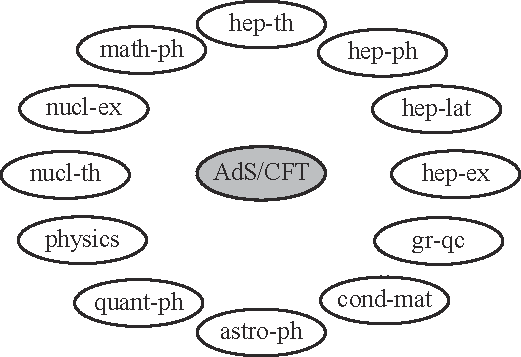
\includegraphics{Ch1_arXiv.pdf} }
\vskip2mm
\caption{The AdS/CFT duality spans all physics arXivs.}%�A�[�J�C�u�ɂ܂�����AdS/CFT�o�ΐ�
\label{fig:arXiv}
\end{figure}%
%%============


The AdS/CFT duality originated from string theory, so it had been discussed in string theory. But the situation is changing in recent years, and AdS/CFT has been discussed beyond theoretical particle physics. This is because AdS/CFT is becoming a powerful tool to analyze the ``real-world." Examples are QCD, nuclear physics, nonequilibrium physics, and condensed-matter physics. In fact, the original AdS/CFT paper \cite{Maldacena:1997re2} has been cited in \textit{all} physics arXivs (\fig{arXiv}). 
%���Ƃ���AdS/CFT�͒������_�̍l���Ȃ̂ŁC�������_�̕���Ő���ɋc�_����Ă����D�������C�ߔN�͗l�����ς���Ă��Ă���CAdS/CFT�͑f���q�_�̘g�𒴂��ċc�_����Ă��Ă���D����́CAdS/CFT���u�������E�v����͂��邤���ŋ��͂Ȏ�@�ɂȂ�‚‚��邩��ł���D���p����Ƃ��ẮCQCD�C���q�j�����C�����_�C���̗͊w�i�񕽍t���v�͊w�j�Ȃǂ���������D�v���v�����g�E�T�[�o�[�i�A�[�J�C�u�j�Ō������Ă݂�ƁC�A�[�J�C�u�̕������삷�ׂĂ�AdS/CFT�̘_�� \cite{Maldacena:1997re} �����p����Ă���i\fig{arXiv}�j�D

For example, the theoretical foundation behind the strong force has been well-understood as QCD. But the perturbation theory often fails because the strong force is literally strong. However, according to AdS/CFT, one can analyze a strongly-coupled gauge theory using the AdS spacetime. So, there are many attempts to analyze the strong force using AdS/CFT%
\footnote{QCD is a $SU(3)$ gauge theory, but AdS/CFT typically considers a $SU(N_c)$ supersymmetric gauge theory, so one should note that AdS/CFT gives only approximate results.}.
%���Ƃ��΁C�����͂̏ꍇ�C���̗��_�I��b�͗ʎq�F�͊w�Ƃ��ė�������Ă��邪�C�����͕͂����ǂ��苭�����߁C�ۓ��_�͂��܂���ɗ����Ȃ��󋵂������D�������CAdS/CFT�ɂ��΁CAdS������g�����Ƃŋ������̃Q�[�W���_����͂ł���D�����ŁCAdS/CFT���g���������͂̉�͂������ɂ����Ȃ��Ă���%
%\footnote{�����Ƃ��C�ʎq�F�͊w��$SU(3)$�Q�[�W���_�����CAdS/CFT�ł��‚����n�͎��$SU(N_c)$���Ώ̃Q�[�W���_�ł���D���������āCAdS/CFT�̌��ʂ͋ߎ��I�Ȍ��ʂł���D}�D

% added
One such example is the \keyword{quark-gluon plasma} (QGP). According to QCD, the fundamental degrees of freedom are not protons or neutrons but \keyword{quarks} and \keyword{gluons}. Under normal circumstances, they are confined inside protons and neutrons. But at high enough temperatures, they are \keyword{deconfined} and form the quark-gluon plasma (\sect{QCD_phase}). The QGP experiments are in progress (\sect{heavy_ion}). According to the experiments, QGP behaves like a fluid with a very small \keyword{shear viscosity}. This implies that QGP is strongly coupled, which makes theoretical analysis difficult (Sects.~\ref{sec:unexpected} and \ref{sec:QGP}). However, it turns out that the value of the viscosity implied by the experiments is very close to the value predicted by AdS/CFT using black holes (\chap{QGP}). This triggers the AdS/CFT research beyond string theory community. 
%1�‚̉��p���{\bf �N�H�[�N�E�O���[�I���E�v���Y�}}\index{�����[������[����ӂ炷��@�N�H�[�N�E�O���[�I���E�v���Y�}�iQGP�j}�iQGP�j�ł���DQCD�ɂ��ƁC�\�������ł�QCD�̊�b�I�Ȏ��R�x�ł���{\bf �N�H�[�N}\index{�����[��@�N�H�[�N}��{\bf �O���[�I��}\index{����[����@�O���[�I��}��{\bf ��‚�����}\index{�ЂƂ�����@��‚�����}���N�����CQGP���Ȃ��i\sect{QCD_phase}�j�D���̎������i�s���ł���i\sect{heavy_ion}�j�D�����ɂ��ƁCQGP��{\bf ����S����}\index{����˂񂹂����@����S����}�̏��������̂̂悤�ɐU��܂��D���̂��Ƃ́CQGP���������ݍ�p�����Ă��邱�Ƃ��Ӗ����C���_�I�ȉ�͂�������i\ref{sec:unexpected}, \ref{sec:QGP}~�߁j�D�Ƃ��낪�C�������玦�����ꂽ�S���̒l�́C�u���b�N�z�[�����g����AdS/CFT�̗\���l�ɋ߂��i\chap{QGP}�j�D���̂��߁C����𒴂���AdS/CFT���c�_�����悤�ɂȂ����D

%%============
\begin{figure}[tb]
\centering
%\hspace{0.25in}
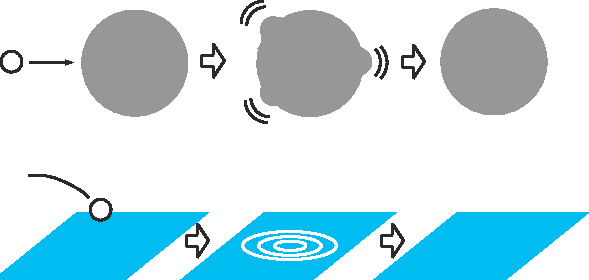
\includegraphics{Ch1_hydro.pdf}
\vskip2mm
\caption{When one adds perturbations, a black hole behaves like a hydrodynamical system. In hydrodynamics, the dissipation is a consequence of viscosity.}
% �ۓ���^�����Ƃ��C�u���b�N�z�[���̂ӂ�܂��͗��̗͊w�̂ӂ�܂��Ƃ悭���Ă���D���̗͊w�ł́C����͔S���̌��ʂł���}
\label{fig:hydro}
\end{figure}%
%%============

How is the black hole related to the viscosity? Here, we give an intuitive explanation (\fig{hydro}). Consider adding a perturbation to a thermal system which is in equilibrium. For example, drop a ball in a water pond. Then, surface waves are generated, but they decay quickly, and the water pond returns to a state of stable equilibrium. This is a \keyword{dissipation} which is a consequence of viscosity. 

This behavior is very similar to a black hole. Again, drop an object to a black hole. Then, the shape of the black hole horizon becomes irregular, but such a perturbation decays quickly, and the black hole returns to the original symmetric shape. If one regards this as a dissipation as well, the dissipation occurs since the perturbation is absorbed by the black hole. Thus, one can consider the notion of viscosity for black holes as well, and the ``viscosity" for black holes should be calculable from the above process. 
%�u���b�N�z�[���ƔS�����ǂ��֌W������̂��C���[�W�������Ă��炤���߂ɁC���ϓI�Ȑ��������Ă������i\fig{hydro}�j�D���t��Ԃɂ���M�͊w�n�ɁC�Ȃɂ��ۓ���^���邱�Ƃɂ��悤�D���Ƃ��΁C�r�Ƀ{�[���𗎂Ƃ��Ƃ����g�����‚��C�����g�͂₪�Ď~��ł��Ƃ̐Â��Ȑ��ʂɖ߂�D����{\bf �U��}\index{���񂢂�@�U��}�́C�S���ɂ����ʂł���D

%�u���b�N�z�[���̂ӂ�܂����C���̂Ǝ��Ă���D��͂�C�u���b�N�z�[���Ƀ��m�𗎂Ƃ����Ƃ��悤�D����ƁC���΂炭�̊ԁC�u���b�N�z�[���̌`�͕s�K���ɂȂ邪�C�ŏI�I�ɂ͂��Ƃ̑Ώ̓I�ȃu���b�N�z�[���ɖ߂��Ă��܂��D��������̎U��Ƃ݂Ȃ��ƁC���̏ꍇ�̎U��͐ۓ����u���b�N�z�[���ɋz������邱�Ƃɂ���ċN����D���������āC�u���b�N�z�[���ɑ΂��Ă��Ȃɂ��S���̂悤�ȊT�O���l������͂��ŁC���́u�S���v�͏�̂悤�ȃv���Z�X���l����Όv�Z�ł��邾�낤�D

% added
Such a phenomenon is in general known as a \keyword{relaxation phenomenon}. In a relaxation phenomenon, one adds a perturbation and sees how it decays. The relaxation phenomenon is the subject of \keyword{nonequilibrium statistical mechanics} or \keyword{hydrodynamics}. The important quantities there are \keyword{transport coefficients}. The viscosity is an example of transport coefficients. A transport coefficient measures how some effect propagates. The correspondence between black holes and hydrodynamics may sound just an analogy, but one can indeed regard that black holes have a very small viscosity; one purpose of this book is to show this.
%���̂悤��{\bf �ɘa����}\index{����킯�񂵂悤@�ɘa����}�́C{\bf �񕽍t���v�͊w}\index{�Ђւ������Ƃ������肫����@�񕽍t���v�͊w}��{\bf ���̗͊w}\index{��䂤�����肫����@���̗͊w}�̃e�[�}�ł���C�傽�镨���ʂ�{\bf �A���W��}\index{�䂻����������@�A���W��}�ł���i\chap{hydro}�j�D�S�����A���W����1�‚ł���D�u���b�N�z�[���Ɨ��̂Ƃ̑Ή��͒P�Ȃ�A�i���W�[�ɂ����Ȃ��悤�Ɏv���邩������Ȃ����C���ۂɃu���b�N�z�[���������ȔS�������‚Ƃ݂Ȃ��邱�Ƃ������̂��{���̖ڕW��1�‚ł���D

The AdS/CFT applications are not limited to QCD. Strongly-coupled systems often arise in condensed-matter physics such as high-$T_c$ superconductivity (\sect{Hi-Tc}). Partly inspired by the ``success" of AdS/QGP, researchers try to apply AdS/CFT to condensed-matter physics (\chap{phase}).
%�܂��C�����ł����΂��΋����֌n���������i���Ƃ��΍������`��\index{�������񂿂悤�Ă�Ƃ�@�������`��}�Ȃǁj�D�����������󋵂��󂯂āCAdS/CFT�𕨐��_�ɉ��p���悤�Ƃ�������������ɂ����Ȃ��Ă���i\chap{phase}�j�D

As one can see, the applications of AdS/CFT has the ``cross-cultural" character, so researchers in other fields often initiated new applications. For example, the applications of AdS/CFT to the quark-gluon plasma were initiated by nuclear physicists. As another example, the Fermi surface was first discussed in AdS/CFT by a condensed-matter physicist.
%���̂悤�ɕ��쉡�f�I�Ȍ����̐��i����C���̎�̉��p�ł́C���΂��Α�����̌����҂����������[�h���Ă����D���Ƃ��΁C���q�j�����̌����҂ɂ���āCAdS/CFT���N�H�[�N�E�O���[�I���E�v���Y�}�ɉ��p���悤�Ƃ������ꂪ�͂��܂����D�܂����������̌����҂ɂ���āCAdS/CFT�Ńt�F���~�ʂ��͂��߂ċc�_���ꂽ�D


%%%%%%%%%
\section{Outline}%\label{sec:}
%%%%%%%%%

This book describes applications of AdS/CFT, but it is not our purpose to cover \textit{all} applications of AdS/CFT. This is because so many applications exit and new applications have been proposed very often. We would rather explain the basic idea than cover all applications. Then, as examples, we discuss  following applications:
\begin{itemize}
\item \chap{wilson}: Wilson loops, or quark potentials
%\item \sect{r-charged}: current anomaly
\item \chap{QGP}: application to QGP (transport coefficients)
\item \sect{2nd_order}: application to hydrodynamics (second-order hydrodynamics)
\item \sect{H^3}: \HSC
\end{itemize}
%as typical applications, we explain applications to the quark-gluon plasma or the so-called holographic superconductors. 
But once one gets accustomed to the basic idea, it is not very difficult to apply AdS/CFT to various systems. Essentially what one should do is to repeat a similar exercise.
%�{���ł�AdS/CFT�̉��p��������邪�CAdS/CFT�̉��p��ԗ����邱�Ƃ͖ړI�ł͂Ȃ��D���̎�̉��p�͖c��Ȑ��ɏ��C�܂����X�V�������p����Ă���Ă��邩��ł���D�����X�̃g�s�b�N���Љ����C��{�I�ȍl���������������������D�����āCAdS/CFT�̉��p�̓T�^��Ƃ��āC�N�H�[�N�E�O���[�I���E�v���Y�}�ւ̉��p��C�z���O���t�B�b�N���`���ƌĂ΂��g�s�b�N�Ȃǂ��������D�������C���������{�I�ȍl���𗝉�����������΁C���܂��܂Ȍn�ɉ��p���邱�Ƃ͓���͂Ȃ��D��{�I�ɂ͓����悤�Ȍv�Z�̌J��Ԃ��ɂ����Ȃ�����ł���D

This book assumes knowledge on elementary general relativity and elementary field theory but does not assume knowledge on black holes and string theory. Also, AdS/CFT has been applied to many different areas of physics, so we explain basics of each area: 
%�{���ł͈�ʑ��Θ_���̗��_�ɂ‚��Ă͏����I�Ȓm�������肵�Ă��邪�C�u���b�N�z�[���⒴�����_�ɂ‚��Ă̒m���͉��肵�Ȃ��D�܂��CAdS/CFT�̉��p�͑�����ɂ킽��̂ŁC���܂��܂ȕ���̊�b�m����������‚‹c�_��i�߂�F
\begin{itemize}
\item Chap.~\ref{chap:BH} and \ref{chap:BH_thermodynamics}: black holes, black hole thermodynamics
\item \chap{QCD}: quantum chromodynamics
\item \chap{string}: superstring theory
\item \chap{hydro}: nonequilibrium statistical mechanics, hydrodynamics
\item \chap{GL}: condensed-matter physics
\end{itemize}
The readers with enough backgrounds may skip some of these chapters.
%\footnote{It is not our main purpose however to explain these background knowledge themselves, so experts may find them insufficient. %A disclaimer: I am not the expert in all these fields. If you find some mistakes, please let me know. }.
%���ꂼ��̊�b�m�����������ǎ҂́C�Y������͂��Ƃ΂��ēǂ�ł������‚����Ȃ�%
%\footnote{�Ȃ��C�{���̖ړI�͂����̉�����̂��ړI�ł͂Ȃ��̂ŁC���Ƃɂ͕�����Ȃ��_�����邩������Ȃ��D�܂��C�M�҂͂���炷�ׂĂ̕���̐��ƂƂ����킯�ł��Ȃ��̂ŁC����Ă���_�����邩������Ȃ��D�����̓_�ɂ‚��ẮC���w�E����������΍K���ł���D}�D

All chapters end with a list of keywords, and most chapters have a summary. After you read each chapter, you could check your understanding by trying to explain those keywords.
% corrected/modified
Also, there are exercises in \chap{exercise}. Some are easy, and their aim is to check your understanding. Some are more involved, and their aim is to delve into discussion in the text. Some exercises need knowledge of advanced sections (Sections with ``~\advanced~") as prerequisite, but in such a case, we mention it explicitly. 

This book devotes some pages to explain how one reaches AdS/CFT. But some readers may first want to get accustomed to AdS/CFT through actual computations. In such a case, one would skip \sect{large_N} and \chap{string}.
%``it is better to accustom yourself to it than to learn it." 
%�܂��C�{���ł͂ǂ̂悤�ɂ���AdS/CFT�̍l�����ɂ��ǂ蒅�����̂��Ƃ��������ɂ��y�[�W�������Ă��邪�C����u�K����芵���v�Ŏ��ۂ̌v�Z��ʂ���AdS/CFT�𗝉����Ă��������ǎ҂����邾�낤�D�����������ꍇ�C\sect{large_N}�C\chap{string}���Ƃ΂��ēǂނ̂���Ăł���D

Sections and footnotes with ``~\advanced~" are somewhat advanced topics and may be omitted in a first reading.
%\advanced ���‚��Ă���߂�r���́C���i�񂾃g�s�b�N�ł���C�ŏ��ɓǂނƂ��͂Ƃ΂��Ă������‚����Ȃ��D

%%%%%%%%%
\section{Notation and conventions}\label{sec:notations}
%%%%%%%%%

We use the natural units $\hbar=c=1$. We often set the Boltzmann constant $k_\text{B} =1$ for thermodynamic analysis. We restored these constants in some sections though.
%�{���ł� $\hbar=c=1$ �̎��R�P�ʌn���g���D�܂��C�M�͊w�I�ȋc�_�ł́C�{���c�}���萔 $k_\text{B} =1$ �̒P�ʌn�����΂��Ύg���D�������C�����‚��̐߂ł͂����̒P�ʌn�͗p�����C���ׂĂ̒萔�������ɏ������Ƃ�����D

We use the metric signature $(-,+, \ldots, +)$, which is standard in general relativity and in string theory. We follow Ref.~\cite{MTW} for the quantities made from the metric, such as the Christoffel symbols and curvature tensors. 
%�v�ʂ̕����isignature�j�́C��ʑ��Θ_�⌷���_�ŕW���I�ɗp������ $(-,+, \ldots, +)$ �̋K����g���D�܂��v�ʂ������鏔�ʁC�N���X�g�b�t�F���L���⃊�[�}���E�e���\���Ȃǂ̋K��͕���~\cite{MTW}�ɂ��������D
For vector and tensor components, we use Greek indices $\mu, \nu, \ldots$ following the standard convention in general relativity \textit{until \sect{reexamination}.} However, in this book, we have the four-dimensional spacetime where a gauge theory lives and the five-dimensional spacetime where a gravitational theory lives, and we have to distinguish which spacetime dimensions we are talking of. Starting from \sect{reexamination},
 %�x�N�g���C�e���\���Ȃǂ̓Y���ɑ΂��āC\sect{reexamination}�܂ł͈�ʑ��Θ_�̕W���I�ȋK��ɂ��������C�M���V�������̓Y�� $\mu,\nu,\ldots$ ���g���D�������C�{���ł̓Q�[�W���_�̏Z��4��������Əd�͗��_�̏Z��5�������󂪏o�Ă���̂ŁC�Y�����ǂ���̈Ӗ��Ŏg���Ă���̂���ʂ���K�v������D\sect{reexamination}�ȍ~�́C
\begin{itemize}
\item
Greek indices $\mu, \nu, \ldots$ run though $0,\ldots,3$ and are used for \textit{the four-dimensional spacetime where a gauge theory lives}. We write boundary coordinates in several ways: $x=x^\mu=(t,\bmx)=(t,x,y,z)$.

\item
Capital Latin indices $M, N, \ldots$ run though $0,\ldots,4$ and are used for \textit{the five-dimensional spacetime where a gravitational theory lives}.
%�M���V�������̓Y�� $\mu,\nu,\ldots$ �́C{\bf �Q�[�W���_�̏Z��4��������ɑ΂��Ďg��}�C$0,\ldots,3$ �܂ő�����̂Ƃ���D
%����C�啶���A���t�@�x�b�g�̓Y�� $M,N,\ldots$ �́C{\bf �d�͗��_�̏Z��5��������ɑ΂��Ďg��}�C$0,\ldots,4$ �܂ő�����̂Ƃ���D
\end{itemize}

In field theory, both the Lorentzian formalism and the Euclidean formalism exit. AdS/CFT has both formalisms as well. The Euclidean formalism is useful to discuss an equilibrium state whereas the Lorentzian formalism is useful to discuss a nonequilibrium state, so we use both depending on the context, and we try to be careful so that readers are not confused.
%�Ȃ��C��̗��_�Ȃǂł�Lorentzian�莮���ƃ��[�N���b�h�莮����2��ނ���D�{���ł͗�����K�X�g�������Ȃ���c�_��i�߂�i�Ȃ�ׂ��ǎ҂��������Ȃ��悤�ɔz�����邪�j�D���[�N���b�h�莮���͕��t�n���c�_����̂ɕ֗��ł���CLorentzian�莮���͔񕽍t�n���c�_����̂ɕ֗�������ł���D

%%%%%%%%%%%%%%%%%%%%%%
\section{Some useful textbooks and prerequisites}\label{sec:textbooks}
%%%%%%%%%%%%%%%%%%%%%%

For a review article on AdS/CFT, see Ref.~\cite{Aharony:2000ti}. This is a review written in early days of the AdS/CFT research, but this is still the best review available.
%AdS/CFT�̊�{�I�ȑ����񍐂Ƃ��ẮC
%AdS/CFT�����̏��������̂܂Ƃ܂��������񍐂ł���D�c�O�Ȃ���C���܂��ɂ��̑����񍐂𒴂������̂͏o�Ă��Ȃ��D

This book explains the minimum amount of string theory. If one would like to learn more details, see Refs.~\cite{Green:1987sp,Polchinski:1998rq,Zwiebach:2004tj}. 
%�{���ł͕K�v�Œ���̒������_�̒m������������Ȃ����C���ڂ����������_���w�Ԃɂ́C
Reference~\cite{Green:1987sp} is the standard textbook till mid 1990s. Reference~\cite{Polchinski:1998rq} is the standard textbook since then. Reference~\cite{Green:1987sp} is a useful supplement to Ref.~\cite{Polchinski:1998rq} however since the former covers materials which are not covered by the latter. Anyhow, these textbooks are written to grow string theory experts. Advanced undergraduate students and researchers in the other fields may find Ref.~\cite{Zwiebach:2004tj} more accessible. 
%����~[B] ��1990�N��܂ł̕W���I�ȋ��ȏ��C����~[C] �͂���Ȍ�̕W���I�ȋ��ȏ��ł���D����~[B] �́C����~[C] �ł��܂肠�‚����Ă��Ȃ��_�ɂ‚��ďڂ����L�q������C���܂ł����̉��l������D�������C�����̋��ȏ��́C�{�i�I�ɒ������_���C�߂悤�Ƃ���l�����ł���D�w���㋉����C������̐l�ł��ǂ݂₷�����ȏ��Ƃ��ẮC����~[D]  ������D

The other string theory textbooks relatively recently are Refs.~\cite{Becker:2007zj,Kiritsis:2007zz,Johnson:2003gi}.
%���̂ق��̒������_�̋��ȏ��ŁC�ߔN�̂��̂Ƃ��ẮC
These textbooks in recent years cover AdS/CFT. %But, as of writing this book, there is no comprehensive textbook which covers the applications of AdS/CFT.
%�����ߔN�̋��ȏ��ɂ�AdS/CFT�͂Ƃ肠�����Ă���D�������C�{�e���M���_�ŁC�{�������‚����悤��AdS/CFT�̉��p���\���Ɉ��������ȏ��͂Ȃ��D

% corrected/modified
This book explains basics of black holes but assumes basic concepts of general relativity such as metric, curvature, and the Einstein equation as a prerequisite. But, for completeness, we will review them in \chap{BH}. If this is not enough, read textbooks of general relativity \cite{Schutz:1985jx,Zee:2013dea,Wald:1984rg} (\eg, first 8 chapters of \cite{Schutz:1985jx}).
%This book explains basics of black holes but assumes basics of general relativity itself. For textbooks in general relativity, see Refs.~\cite{Schutz:1985jx,Zee:2013dea,Wald:1984rg}.
%�{���ł̓u���b�N�z�[���ɂ‚��Ă͏������������Ă��邪�C��ʑ��Θ_���̂��̂ɂ‚��Ă͏����I�Ȓm�������肵�Ă���D��ʑ��Θ_�̋��ȏ��Ƃ��ẮC
References~\cite{Schutz:1985jx,Zee:2013dea} are elementary textbooks (but Ref.~\cite{Zee:2013dea} is very modern with many advanced topics in recent years), and Ref.~\cite{Wald:1984rg} is an advanced one.
%����~[H] �͏����I�Ȃ��́C����~[I] �͖{�i�I�ȋ��ȏ��ł���D

% corrected/modified
There are many good textbooks of quantum field theory, but we list only a few here in order of increasing difficulty \cite{Ryder:1985wq,Zee:2003mt,Srednicki:2007qs,Peskin:1995ev,Weinberg:1995mt}. It is advisable for readers to have a rough idea about basic concepts of quantum field theory (such as Feynman rules, renormalization, and $\beta$-function using a simple example like the $\phi^4$-theory) and the Abelian gauge theory.

We will mention textbooks in the other fields in appropriate places. 
%�����ȊO�̕���̊�b�m���ɂ‚��ẮC���ȏ���K�X������D
Reading them are not prerequisites though. Those textbooks are mentioned if you would like to learn more details.

Finally, we list review articles and textbooks which cover applications of AdS/CFT \cite{Papantonopoulos:2011zz,Horowitz:2012nnc,DeWolfe:2013cua,Hartnoll:2009sz,McGreevy:2009xe,Iqbal:2011ae,CasalderreySolana:2011us,Ammon:2015wua,Zaanen:2015oix}. These cover the materials which are not covered in this book and are useful complements.


\endofsection

	   \begin{thebibliography}{99}

%
% Chap_intro 
%

%\cite{Maldacena:1997re}
\bibitem{Maldacena:1997re2}
  J.~M.~Maldacena,
  ``The Large N limit of superconformal field theories and supergravity,''
  Adv.\ Theor.\ Math.\ Phys.\  {\bf 2 } (1998)  231
  [hep-th/9711200].

\bibitem{MTW}
%no database entry
C.~W.~Misner, K.~S.~Thorne and J.~A.~Wheeler, 
\textit{Gravitation} 
(W. H. Freeman, 
%San Francisco, 
1973).
%�m�M��F�d�͗��_�i�ۑP�C2011�j�n�D

%\cite{Aharony:2000ti}
\bibitem{Aharony:2000ti}
O.~Aharony, S.~S.~Gubser, J.~Maldacena, H.~Ooguri and Y.~Oz,
``Large N field theories, string theory and gravity,''
Phys.\ Rept.\  {\bf 323} (2000) 183
[hep-th/9905111].
%%CITATION = HEP-TH 9905111;%%

%\cite{Green:1987sp}
\bibitem{Green:1987sp}
  M.~B.~Green, J.~H.~Schwarz and E.~Witten,
  \textit{Superstring theory}
  (Cambridge Univ.\ Press, 1987).
    
%\cite{Polchinski:1998rq}
\bibitem{Polchinski:1998rq}
  J.~Polchinski,
  \textit{String theory}
  (Cambridge Univ.\ Press, 1998).

%\cite{Zwiebach:2004tj}
\bibitem{Zwiebach:2004tj}
  B.~Zwiebach,
  \textit{A first course in string theory, second edition}
  (Cambridge Univ.\ Press, 2009).

%\cite{Becker:2007zj}
\bibitem{Becker:2007zj}
  K.~Becker, M.~Becker and J.~H.~Schwarz,
  \textit{String theory and M-theory: A modern introduction}
  (Cambridge Univ.\ Press, 2007).

%\cite{Kiritsis:2007zz}
\bibitem{Kiritsis:2007zz}
  E.~Kiritsis,
  \textit{String theory in a nutshell}
  (Princeton Univ.\ Press, 2007).
  
%\cite{Johnson:2003gi}
\bibitem{Johnson:2003gi}
  C.~V.~Johnson,
  \textit{D-branes}
  (Cambridge Univ.\ Press, 2003).   

%\cite{Schutz:1985jx}
\bibitem{Schutz:1985jx}
B.~F.~Schutz,
\textit{A first course in general relativity, second edition}
(Cambridge Univ.\ Press, 2009).
%�m�M��F�o�[�i�[�h�E�e�E�V���b�c�C���Θ_���� ��2�Łi�ۑP�C2010�j�n�D

%\cite{Zee:2013dea}
\bibitem{Zee:2013dea}
A.~Zee,
\textit{Einstein Gravity in a Nutshell}
(Princeton Univ.\ Press, 2013).

%\cite{Wald:1984rg}
\bibitem{Wald:1984rg}
R.~M.~Wald,
\textit{General relativity}
(The Univ.\ of Chicago Press, 1984).

% added
%\cite{Ryder:1985wq}
\bibitem{Ryder:1985wq}
  L.~H.~Ryder,
  \textit{Quantum Field Theory, second edition} 
  (Cambridge Univ.\ Press, 1996).
  
% added
%\cite{Zee:2003mt}
\bibitem{Zee:2003mt}
  A.~Zee,
  \textit{Quantum field theory in a nutshell}
  (Princeton Univ.\ Press, 2010).

% added
%\cite{Srednicki:2007qs}
\bibitem{Srednicki:2007qs}
  M.~Srednicki,
  \textit{Quantum field theory}
  (Cambridge Univ.\ Press, 2007).
  
% added
%\cite{Peskin:1995ev}
\bibitem{Peskin:1995ev}
  M.~E.~Peskin and D.~V.~Schroeder,
  \textit{An Introduction to quantum field theory}
  (Addison-Wesley, 1995).
  
% added
%\cite{Weinberg:1995mt}
\bibitem{Weinberg:1995mt}
  S.~Weinberg,
  \textit{The Quantum theory of fields}, Vol. 1-3
  (Cambridge Univ.\ Press, 1995-2000).
%The Quantum theory of fields. Vol. 1: Foundations,''

%\cite{Weinberg:1996kr}
%\bibitem{Weinberg:1996kr}
%  S.~Weinberg,
%``The quantum theory of fields. Vol. 2: Modern applications,''

%\cite{Weinberg:2000cr}
%\bibitem{Weinberg:2000cr}
%  S.~Weinberg,
  %``The quantum theory of fields. Vol. 3: Supersymmetry,''

%\cite{Papantonopoulos:2011zz}
\bibitem{Papantonopoulos:2011zz}
\textit{From Gravity to Thermal Gauge Theories: The AdS/CFT Correspondence}, 
eds. E. Papantonopoulos, Lecture Notes in Physics 828 (Springer, 2011).

%\cite{Horowitz:2012nnc}
\bibitem{Horowitz:2012nnc}
\textit{Black Holes in Higher Dimensions}, 
eds. G. Horowitz (Cambridge University Press, 2012).

%\cite{DeWolfe:2013cua}
\bibitem{DeWolfe:2013cua}
  O.~DeWolfe, S.~S.~Gubser, C.~Rosen and D.~Teaney,
  ``Heavy ions and string theory,''
  arXiv:1304.7794 [hep-th].
  %%CITATION = ARXIV:1304.7794;%%

% added
%\cite{Hartnoll:2009sz}
\bibitem{Hartnoll:2009sz}
  S.~A.~Hartnoll,
  ``Lectures on holographic methods for condensed matter physics,''
  Class.\ Quant.\ Grav.\  {\bf 26} (2009) 224002
  [arXiv:0903.3246 [hep-th]].
  %%CITATION = ARXIV:0903.3246;%%
  
% added
%\cite{McGreevy:2009xe}
\bibitem{McGreevy:2009xe}
  J.~McGreevy,
  ``Holographic duality with a view toward many-body physics,''
  Adv.\ High Energy Phys.\  {\bf 2010} (2010) 723105
  [arXiv:0909.0518 [hep-th]].
  %%CITATION = ARXIV:0909.0518;%%

%\cite{Iqbal:2011ae}
\bibitem{Iqbal:2011ae}
  N.~Iqbal, H.~Liu and M.~Mezei,
  ``Lectures on holographic non-Fermi liquids and quantum phase transitions,''
  arXiv:1110.3814 [hep-th].
  %%CITATION = ARXIV:1110.3814;%%

%\cite{CasalderreySolana:2011us}
\bibitem{CasalderreySolana:2011us}
  J.~Casalderrey-Solana, H.~Liu, D.~Mateos, K.~Rajagopal and U.~A.~Wiedemann,
  \textit{Gauge/String Duality, Hot QCD and Heavy Ion Collisions} (Cambridge Univ.\ Press, 2014)
  [arXiv:1101.0618 [hep-th]].
  %%CITATION = ARXIV:1101.0618;%%

% added
%\cite{Ammon:2015wua}
\bibitem{Ammon:2015wua}
  M.~Ammon and J.~Erdmenger,
  \textit{Gauge/gravity duality : Foundations and applications}
  (Cambridge Univ.\ Press, 2015).
  %%CITATION = INSPIRE-1376202;%%

% added
%\cite{Zaanen:2015oix}
\bibitem{Zaanen:2015oix}
  J.~Zaanen, Y.~W.~Sun, Y.~Liu and K.~Schalm,
  \textit{Holographic Duality in Condensed Matter Physics}
  (Cambridge Univ.\ Press, 2015).
  %%CITATION = INSPIRE-1384852;%%

\end{thebibliography}

	%\documentclass[11pt]{jarticle} %%% �A���R�����g
\ifx\nameofpaper\undefined %%% ���� main.tex ���ǂ܂�Ă��Ȃ����
  \usepackage{macro_natsuume} %%% �����p�̃}�N���t�@�C����ǂݍ��݁C
  \def\beginsection{\section*}
  \def\endofsection{\end{document}} %%% \endofsection = \bye �ƒ�`
  \input draft_header.tex
\else %%% �����łȂ����
  \def\beginsection{\chapter}
  \def\endofsection{\endinput} %%% \endofsection = \endinput �ƒ�`
\fi


%%%%%%%%%
\beginsection{General relativity and black holes
%��ʑ��Θ_�ƃu���b�N�z�[��
}\label{chap:BH}
%%%%%%%%%

%\begin{flushright}
%        \today\\
%\end{flushright}

\begin{quote}
In this book, black holes frequently appear, so we will describe the simplest black hole, the Schwarzschild black hole and its physics.
%�{���ł̓u���b�N�z�[�����p�ɂɓo�ꂷ��̂ŁC�܂������Ƃ��ȒP�ȃu���b�N�z�[���C�V�������c�V���h�E�u���b�N�z�[���ɂ‚��Đ������C�V�������c�V���h�E�u���b�N�z�[���ł̕����𒲂ׂ�D
\end{quote}
%\vskip10pt

Roughly speaking, a black hole is a region of spacetime where gravity is strong so that even light cannot escape from there. The boundary of a black hole is called the \keyword{horizon}. Even light cannot escape from the horizon, so the horizon represents the boundary between the region which is causally connected to distant observers and the region which is not. 
%�傴���ςɌ����āC�u���b�N�z�[���Ƃ͏d�͂������Ȃ�C���������O�ɏo���Ȃ��̈�̂��Ƃł���D�����āC�u���b�N�z�[���̋��E��{\bf �z���C�Y��}\index{�ق炢����@�z���C�Y��}�ihorizon�j�ƌĂԁD�z���C�Y������͌�������������Ȃ��̂ŁC�z���C�Y���̓u���b�N�z�[���̓�����O�ֈ��ʓI�ȉe��������Ԍ��E�ł���D

General relativity is mandatory to understand black holes properly, but a black hole-like object can be imagined in Newtonian gravity. Launch a particle from the surface of a star, but the particle will return if the velocity is too small. In Newtonian gravity, the particle velocity must exceed the escape velocity in order to escape from the star. From the energy conservation, the escape velocity is determined by
%�u���b�N�z�[���𐳊m�ɗ�������ɂ́C��ʑ��Θ_���������Ȃ����C�u���b�N�z�[���̂悤�Ȃ��̂̑��݂́C�j���[�g���͊w�I�ȋc�_������z�����邱�Ƃ��ł���D���̂𐯂̕\�ʂ��瓊���グ���Ƃ��C���x���������Əd�͂ɂ���Đ��ɖ߂��Ă��܂��D�j���[�g���͊w�ł́C���̏d�͂��瓦��邽�߂ɂ͒E�o���x�𒴂��Ă���K�v������D�E�o���x�́C�G�l���M�[�ۑ�������C
\be
%
\frac{1}{2}v^2=\frac{GM}{r}~.
%\label{eq:}
%
\ee
%�ɂ���Č��܂�D
If the radius $r$ becomes smaller for a fixed star mass $M$, the gravitational potential becomes stronger, so the escape velocity becomes larger. When the radius becomes smaller, eventually the escape velocity reaches the speed of light. Then, no object can escape from the star. Setting $v=c$ in the above equation gives the radius
%���̎���$M$�������ꍇ�C���a$r$���������Ȃ�قǁC���\�ʂ̏d�͂͋����Ȃ�̂ŁC�E�o���x���傫���Ȃ�D���̔��a������߂ď������Ȃ�ƁC�‚��ɂ͒E�o���x�������x�ɂȂ�D���̂Ƃ��C�ǂ�ȕ��̂ł����Ă��d�͂���͓�����Ȃ��D��̎��� $v=c$ �Ƃ���ƁC���̂Ƃ��̔��a�́C
\begin{equation}
%
r = \frac{2GM}{c^2}~,
\label{eq:horizon}
%
\end{equation}
which corresponds to the horizon. For a solar mass black hole, the horizon radius is about 3 km, which is $2.4\times 10^5$ times smaller than the solar radius. 
%�ŗ^������D���ꂪ�z���C�Y���ɑ�������D���z���x�̏d���̏ꍇ�C�z���C�Y�����a�� 3 km ���x�ɂȂ葾�z���a�� 24 �����̂P�����Ȃ��D

To be precise, the above argument is false from several reasons:
%�����‚��̗��R����C���m�ɂ͂��̂悤�ȋc�_�͌��ł���F
\begin{enumerate}

\item
First, the speed of light is arbitrary in Newtonian mechanics. As a result, the speed of light decreases as light goes away from the star. But in special relativity the speed of light is the absolute velocity which is independent of observers. 
%�܂��C�j���[�g���͊w�I�ȋc�_�ł͌����x�͔C�ӂł���D���̌��ʂƂ��āC���̂悤�ȋc�_�ł́C�u���b�N�z�[�����痣���ɂ‚�Č��̑��������邱�ƂɂȂ�D���������ꑊ�Θ_�ł͌����x�͐�Α��x�ł���C�ǂ̊ϑ��҂ɂƂ��Ă���ӓI�Ȓl�����D
\item
Newtonian mechanics cannot determine how gravity affects light.
%�܂��C���������j���[�g���͊w�ł͏d�͂����ɂǂ��e������̂��͌��߂��Ȃ��D
\item
In the above argument, light can temporally leave from the ``horizon." But in general relativity light cannot leave even temporally.
%����ɁC�j���[�g���͊w�ł͌����E�o�ł����߂��ė���ɂ���C�ꎞ�I�Ɂu�z���C�Y���v����E�o�ł��Ȃ��킯�ł͂Ȃ��D�������C��ʑ��Θ_�ɂ��ƁC�z���C�Y����������ꎞ�I�ɂ���E�o���邱�Ƃ͂Ȃ��D
\end{enumerate}
The Newtonian argument has various problems, but the horizon radius \eqref{eq:horizon} itself remains true in general relativity, and we utilize Newtonian arguments again later. 
%���̂悤�ɁC�j���[�g���͊w�I�ȋc�_�ɂ͑��X��肪������̂́C�z���C�Y�����a�̎� \eqref{eq:horizon} �͈�ʑ��Θ_�ɂ����Ă����̂܂ܐ��藧�D�j���[�g���͊w�I�ȋc�_�ɂ‚��ẮC�܂����Ƃł����p����D

Below we explain black holes using general relativity, but we first discuss the particle motion in a given spacetime. For the flat spacetime, this is essentially a review of special relativity. We take this approach from the following reasons: (i) We study the particle motion around black holes later in order to understand black hole physics; (ii) The main purpose of this book is not to obtain a new geometry but to study the behavior of a ``probe" such as a particle in a known geometry; (iii) String theory is a natural extension of the particle case below.
%�ȉ��C��ʑ��Θ_��p���ău���b�N�z�[�����c�_���邪�C�܂��^����ꂽ����ŗ��q�̉^�����ǂ��L�q���邩�C����o�����邱�Ƃɂ���i���R�Ȏ���̏ꍇ�C����͎����I�ɂ͓��ꑊ�Θ_�̂����炢�ł���j�D����́C�u���b�N�z�[���̕����𗝉����邽�߂ɁC���ƂŃu���b�N�z�[������ł̗��q�̉^���𒲂ׂ邩��ł���D�܂��C�{���ł͎�����ǂ����߂邩�ł͂Ȃ��C�ނ�����m�̎���ɗ��q�̂悤�ȁu�v���[�u�v���������Ƃ��̃v���[�u�̐U��܂��𒲂ׂ邱�Ƃ����Ƃ��Ă���̂ŁC���̂悤�ȃA�v���[�`�����R�ł���D����ɁC�������_�̌��݂̒莮�����C���q�̏ꍇ�����R�Ɋg���������̂ɂȂ��Ă���D


%%%%%%%%%
\section{Particle action
%���q�̍�p
}%\label{sec:}
%%%%%%%%%

%%------------------
\subsubsection*{Flat spacetime case --- review of special relativity
%���R�Ȏ���̏ꍇ---���ꑊ�Θ_�̂����炢
}\label{sec:particle_action_flat}
%%------------------

First, let us consider the particle motion in the flat spacetime. We denote the particle's coordinates as $x^\mu:=(t,x,y,z)$. According to special relativity, the distance which is invariant relativistically is given by
%�܂��͕��R�Ȏ���ł̗��q�̉^�����l���悤�D���q�̍��W�� $x^\mu:=(t,x,y,z)$ �Ƃ���D���ꑊ�Θ_�ɂ��ƁC���q�ɂƂ��đ��Θ_�I�ȕs�ϋ�����
\be
%
ds^2 = - dt^2 + dx^2 + dy^2 + dz^2~.
%\label{eq:}
%
\ee
The distance is called timelike when $ds^2<0$, spacelike when $ds^2>0$, and null when $ds^2=0$. For the particle, $ds^2<0$, so one can use the \keyword{proper time} $\tau$ given by
%�ł���D2�_�Ԃ̋����� $ds^2<0$ �̏ꍇ�C2�_�Ԃ̊֌W�����ԓI�itimelike�j�ƌĂсC$ds^2>0$ ����ԓI�ispacelike�j�C$ds^2=0$ ���k���inull�j�ƌĂԁD���q�ɑ΂��Ă�$ds^2<0$�Ȃ̂�
\be
%
ds^2 = - d\tau^2~.
%\label{eq:}
%
\ee
%�ŗ^������{\bf �ŗL����}\index{���䂤������@�ŗL����}�iproper time�j$\tau$ ���g���Ă��悢�D

The proper time gives the relativistically invariant quantity for the particle, so it is natural to use the proper time for the particle action:
%���q�ɂƂ��ČŗL���Ԃ����Θ_�I�ȕs�ϗʂȂ̂ŁC���q�̍�p���ŗL���Ԃŏ����̂����R�ł���F
\be
%
\action = - m \int d\tau~.
\label{eq:action_particle1}
%
\ee
The action takes the familiar form in the nonrelativistic limit. With the velocity $v^i := dx^i/dt$, $d\tau$ is written as $d\tau = dt (1-v^2)^{1/2}$, so
%�񑊑Θ_�I�Ɍ����l����ƁC���̍�p�����R�ł��邱�Ƃ��݂ĂƂ邱�Ƃ��ł���D ���x $v^i := dx^i/dt$ ��p����ƁC$d\tau = dt (1-v^2)^{1/2}$ �Ȃ̂�
\be
%
\action = - m \int dt (1-v^2)^{1/2}
\simeq -m \int dt \left(1 - \frac{1}{2}v^2 + \cdots \right), \quad (v \ll 1)~.
%\label{eq:}
%
\ee
In the final expression, the first term represents the particle's rest mass energy, and the second term represents the nonrelativistic kinetic energy. 
%�ʼnE�ӂ̎��ŁC��ꍀ�͗��q�̐Î~�G�l���M�[�C��񍀂͔񑊑Θ_�I�ȉ^���G�l���M�[������킵�Ă���D

%%============
\begin{figure}[tb]
\begin{center}
\scalebox{0.75}{ 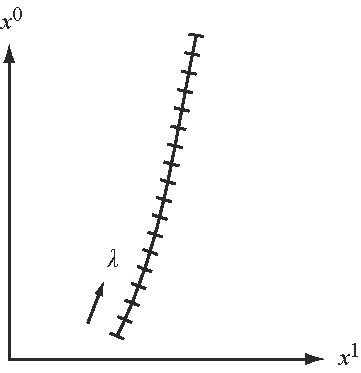
\includegraphics{Ch2_world_line.pdf} }
\vskip2mm
\caption{A particle draws a world-line in spacetime}
%���q�͎��󒆂Ő��E����|���D
\label{fig:world_line}
\end{center}
\end{figure}
%%============

A particle draws a \keyword{world-line} in spacetime (\fig{world_line}). Introducing an arbitrary parametrization $\lambda$ along the world-line, the particle coordinates or the particle motion are described by $x^\mu(\lambda)$. Using the parametrization, 
%���q�͎��󒆂�{\bf ���E��}\index{����������@���E��}�iworld-line�j��|���i\fig{world_line}�j�D���E���ɉ������C�Ӄp�����[�^ $\lambda$ �𓱓�����ƁC���q�̍��W�C�‚܂藱�q�̉^���� $x^\mu(\lambda)$ �ɂ���Ďw�肷�邱�Ƃ��ł���D���̃p�����[�^���g����
\be
%
d\tau^2 
= - \eta_{\mu\nu} dx^\mu dx^\nu 
= - \eta_{\mu\nu} \dotx^\mu \dotx^\nu d\lambda^2 
\quad (\dot{~} := d/d\lambda)~,
%\label{eq:}
%
\ee
so the action is written as
%�Ȃ̂ŁC��p��
\be
%
\action = -m \int d\lambda\, \sqrt{ -\eta_{\mu\nu} \dotx^\mu \dotx^\nu } 
= \int d\lambda\, L~.
\label{eq:action_particle2}
%
\ee
The parametrization $\lambda$ is a redundant variable, so the action should not depend on $\lambda$. In fact, the action is invariant under
%�Ə�����������D$\lambda$ �͗]���ȕϐ��Ȃ̂ŁC��p��$\lambda$ �Ɉˑ����ׂ��ł͂Ȃ��D���ہC��p��
\be
%
\lambda' = \lambda' (\lambda)~.
\label{eq:reparametriz_particle}
%
\ee
%�Ƃ����ϊ��̉��ŕs�ςł���D

The canonical momentum of the particle is given by
%���q�̐����^���ʂ�
\be
%
p_\mu = \frac{\del L}{\del \dotx^\mu}
= \frac{ m \dotx_\mu }{ \sqrt{-\dotx^2} }
= m \frac{dx_{\mu}}{d\tau}
%\label{eq:}
%
\ee
($\dotx^2:= \eta_{\mu\nu}\dotx^\mu\dotx^\nu$). Note that the canonical momentum satisfies
%�i$\dotx^2:= \eta_{\mu\nu}\dotx^\mu\dotx^\nu$�j �D�������C�����^���ʂ�
\be
%
p^2 = m^2 \frac{\dotx^2}{-\dotx^2} = -m^2~,
%\label{eq:}
%
\ee
so its components are not independent:
%�𖞂����̂œƗ��ł͂Ȃ��F
\be
%
\boxeq{
p^2 = - m^2~.
}
\label{eq:constraint_on_shell}
%
\ee
The Lagrangian does not contain $x^\mu$ itself but contains only $\dotx^\mu$, so $p_\mu$ is conserved. Thus, $p_\mu = m\, dx_{\mu}/d\tau =\text{(constant)}$, which describes the free motion.
%���O�����W�A��$L$�͍��W $x^\mu$ ���̂��̂͊܂܂� $\dotx^\mu$ �݂̂��܂ނ��߁C$p_\mu$ �͕ۑ�����D���������āC$p_\mu = m\, dx_{\mu}/d\tau =\text{(constant)}$ �ł���C����͎��R�^��������킷�D

The particle's \keyword{four-velocity}\ $u^\mu$ is defined as
%���q��{\bf 4�����x}\index{4���񂻂���@4�����x}$u^\mu$�́C
\be
%
u^\mu := \frac{dx^\mu}{d\tau}~.
%\label{eq:}
%
\ee
In terms of the ordinary velocity $v^i$, 
%�Œ�`�����D���x$v^i$�ŏ����ƁC
\be
%
u^\mu = \frac{dt}{d\tau} \frac{dx^\mu}{dt} = \gamma(1,v^i)~, \quad
\left(\frac{d\tau}{dt}\right)^2 = 1-v^2 := \gamma^{-2}~.
%\label{eq:}
%
\ee
Since $p_\mu = m u_\mu$ and $p^2=-m^2$, $u^\mu$ satisfies $u^2 =-1$.
%$p_\mu = m u_\mu$ ���� $p^2=-m^2$ ���C$u^2 =-1$�ł���D

The action \eqref{eq:action_particle1} is proportional to $m$, and one cannot use it for a massless particle. The action which is also valid for a massless particle is given by
%��p \eqref{eq:action_particle1} �� $m$ �ɔ�Ⴗ�邽�߁C���ʃ[���̗��q�ɑ΂��Ă͈Ⴄ��p���g���K�v������D���ʃ[���̗��q�ɑ΂��Ă����藧��p�Ƃ��Ă�
\be
%
\action = \frac{1}{2}\int d\lambda\, \left\{ e^{-1}  \eta_{\mu\nu} \dotx^\mu \dotx^\nu - e m^2 \right\}~.
\label{eq:action_massless}
%
\ee
From this action,
%���̍�p����
\begin{alignat}{2}
%
&\text{Equation of motion for $e$:} 
& \quad & \dotx^2 + e^2 m^2 = 0~, 
\label{eq:eom_massless1} \\
&\text{Canonical momentum: } 
& \quad & p_\mu = \frac{\del L}{\del \dotx^\mu} = \frac{1}{e} \dotx_\mu 
= \frac{m \dotx_\mu}{ \sqrt{-\dotx^2} }~.
\label{eq:eom_massless2}
%\label{eq:}
%
\end{alignat}
Use \eq{eom_massless1} at the last equality of \eq{eom_massless2}. Using \eq{eom_massless1}, the Lagrangian reduces to the previous one \eqref{eq:action_particle2}:
%\eq{eom_massless2} �̍Ō�̓����ł�\eq{eom_massless1} ���g���D\eq{eom_massless1} ���g���ƁC���O�����W�A���� 
\be
%
\frac{1}{2} \left\{ e^{-1} \dotx^2 - e m^2 \right\}
= - m \sqrt{-\dotx^2}~.
%\label{eq:}
%
\ee
%�ƂȂ�\eq{action_particle2} �ɋA������D

This action also has the reparametrization invariance: the action \eqref{eq:action_massless} is invariant under
%\eq{action_massless} �����W�ϊ��s�ϐ��������C
\begin{align}
%
\lambda' &= \lambda' (\lambda)~, \\
e' &= \frac{d\lambda}{d\lambda'} e~.
%\label{eq:}
%
\end{align}
%�̉��ŁC��p \eqref{eq:action_massless} �͕s�ςɕۂ����D


%%------------------
\subsubsection*{Particle action (curved spacetime)
%���q�̍�p�i�Ȃ���������j
}\label{sec:particle_action_curved}
%%------------------

Now, move from special relativity to general relativity. The invariant distance is given by replacing the flat metric $\eta_{\mu\nu}$ with a curved metric $g_{\mu\nu}(x)$:
%���ꑊ�Θ_�����ʑ��Θ_�Ɉڂ�ƁC���W�s�ςȋ����͕��R�Ȏ���̌v�� $\eta_{\mu\nu}$ �̂����ɋȂ���������̌v�� $g_{\mu\nu}(x)$ ���g��
\be
%
ds^2 = g_{\mu\nu} dx^\mu dx^\nu~.
\label{eq:line_element}
%
\ee
Here, we first consider the particle motion in a curved spacetime and postpone the discussion how one determines $g_{\mu\nu}$.
%�ŗ^������D�v�� $g_{\mu\nu}$ ���ǂ����߂邩�͂��Ƃŋc�_���邱�Ƃɂ��āC�����ł͂܂��Ȃ���������ł̗��q�̉^�����l���邱�Ƃɂ���D

The action is obtained by replacing the flat metric $\eta_{\mu\nu}$ with a curved metric $g_{\mu\nu}$:
%�Ȃ���������ł̗��q�̍�p���C$\eta_{\mu\nu}$ �� $g_{\mu\nu}$ �Œu�������邱�Ƃœ�����F
\be
%
\action = -m \int d\tau
= -m \int d\lambda\, \sqrt{ -g_{\mu\nu}(x) \dotx^\mu \dotx^\nu }~.
%\label{eq:}
%
\ee
Just like the flat spacetime, the canonical momentum is given by
%���R�Ȏ��󓯗l�C�����^���ʂ�
\be
%
p_\mu = m\, \frac{ g_{\mu\nu}(x)\dotx^\nu }{ \sqrt{-\dotx^2} }~, \quad
\dotx^2:= g_{\mu\nu}(x)\dotx^\mu\dotx^\nu~,
%\label{eq:}
%
\ee
and the constraint $p^2 = -m^2$ exists. Also%
\footnote{
What is conserved is $p_\mu$ which may not coincide with $p^\mu$ in general. In the flat spacetime, $p_\mu$ and $p^\mu$ are the same up to the sign, but in the curved spacetime, the functional forms of $p_\mu$ and $p^\mu$ differ by the metric $g_{\mu\nu}(x)$. }, 
%�ŗ^�����C$p^2 = -m^2$ �̍S�����������݂���D�܂�%
%\footnote{�ۑ������̂�$p_\mu$�ł���C��ʂ�$p^\mu$�Ƃ͈�v���Ȃ����Ƃɒ��ӁD���R�Ȏ���ł́C$p_\mu$��$p^\mu$�ɂ͕����̈Ⴂ�����Ȃ����C�Ȃ���������ł͌v�� $g_{\mu\nu}(x)$ �̈��q���Ⴄ�̂ŁC$p_\mu$��$p^\mu$�̊֐��`�͈�v���Ȃ��D}�C
\begin{center}
\fbox{
\begin{tabular}{l}
If the metric is independent of  $x^\mu$, its conjugate momentum  $p_\mu$ is conserved.
%�v�ʂ�������W $x^\mu$ ���܂܂Ȃ��Ƃ��� $p_\mu$ ���ۑ�����D
\end{tabular}
}
\end{center}

The variational principle $\delta \action=0$ gives the world-line which extremizes the action. For the flat spacetime, the particle has the free motion and has the ``straight" world-line. For the curved spacetime, the world-line which extremizes the action is called a \keyword{geodesic}. The variation of the action with respect to $x^\mu$ gives the equation of motion for the particle: 
%�ϕ����� $\delta \action=0$ �́C�ŗL���Ԃ��ɒl���Ƃ鐢�E����^����D���R�Ȏ���̂Ƃ��́C���q�͎��R�^�������C���E���́u�����v�������D�Ȃ���������̏ꍇ�C��p�̋ɒl��^���鐢�E�� $x^\mu(\tau)$ ��{\bf ���n��}\index{����������@���n��}�igeodesics�j�ƌĂԁD��p�� $x^\mu$ �ŕϕ�����ƁC
\be
%
\frac{d^2x^\mu}{d\tau^2} 
+ \Gamma^\mu_{~\rho\sigma} \frac{dx^\rho}{d\tau}\frac{dx^\sigma}{d\tau} = 0~.
\label{eq:geodesic_eq}
%
\ee
This is known as the \keyword{geodesic equation}%
\footnote{
Note that we use the proper time $\tau$ here not the arbitrary parametrization $\lambda$. The equation of motion does not take the form of the geodesic equation for a generic $\lambda$. A parameter such as $\tau$ is called an \keyword{affine parameter}. As one can see easily from the geodesic equation, the affine parameter is unique up to the linear transformation $\tau\rightarrow a\tau+b$ ($a, b$: constant). For the massless particle, the proper time cannot be defined, but the affine parameter is possible to define.
}.
Here, $\Gamma^\alpha_{~\mu\nu}$ is the Christoffel symbol: 
%�Ƃ����^����������������D�����{\bf ���n��������}\index{����������ق��Ă�����@���n��������}�igeodesic equation�j�ƌĂ�%
%\footnote{�����ŔC�ӂ̐��E���p�����[�^$\lambda$�ł͂Ȃ��C�ŗL����$\tau$���g���Ă��邱�Ƃɒ��ӁD�C�ӂ�$\lambda$�ɑ΂��ẮC�^���������͈�ʂɑ��n���������̌`�ɂ͂Ȃ�Ȃ��D$\tau$�̂悤�ȃp�����[�^��{\bf �A�t�B���p�����[�^}\index{���ӂ���͂�߁[��@�A�t�B���p�����[�^}�ƌ����D���n������������ȒP�ɂ킩��悤�ɁC�A�t�B���p�����[�^�ɂ�$\tau\rightarrow a\tau+b$�i$a, b$�F�萔�j�Ƃ������`�ϊ��̎��R�x�����Ȃ��D���ʃ[�����q�ɑ΂��Ă͌ŗL���Ԃ͒�`�ł��Ȃ����̂́C�A�t�B���p�����[�^�̒�`�͉”\�ł���D}�D
%������ $\Gamma^\alpha_{~\mu\nu}$ �̓N���X�g�b�t�F���L��
\be
%
\Gamma^\alpha_{~\mu\nu} = \frac{1}{2}\, g^{\alpha\beta} 
(\del_\nu g_{\beta\mu} + \del_\mu g_{\beta\nu} - \del_\beta g_{\mu\nu})~.
%\label{eq:}
%
\ee
The particle motion is determined by solving the geodesic equation. However, black holes considered in this book have enough number of conserved quantities so that one does not need to solve the geodesic equation.
%�ł���D���n���������������Η��q�̉^�������܂邪�C�ȉ��ł݂�悤�ɁC���̖{�ōl����悤�ȃu���b�N�z�[���ł͏\���Ȑ��̕ۑ��ʂ����邽�߁C���n���������������܂ł��Ȃ��D

The massless particle action is also obtained by substituting $\eta_{\mu\nu}$ with $g_{\mu\nu}$ in  \eq{action_massless}. The particle action described here can be naturally extended into string and the objects called ``branes" in string theory (\sect{NG}). 
%���ʃ[���̗��q�̏ꍇ���C��p \eqref{eq:action_massless} �� $\eta_{\mu\nu} \rightarrow g_{\mu\nu}$ �̒u�������ŗ^������D�����̗��q�̍�p�́C�������_�̃X�g�����O��u���[���Ƃ��������̂ɂ����R�Ɋg���”\�ł���i\sect{NG}�j�D


%%%%%%%%%
\section{Einstein equation and Schwarzschild metric
%�A�C���V���^�C���������ƃV�������c�V���h�v��
}%\label{sec:}
%%%%%%%%%

So far we have not specified the form of the metric, but the metric is determined by the Einstein equation%
\footnote{In \sect{GR}, we summarize the formalism of general relativity for the readers who are not familiar to it.}:
%�����܂Ōv�ʂ̌`�͎w�肹���ɋc�_���Ă������C�v�ʂ̓A�C���V���^�C���������ɂ���Č��܂�%
%\footnote{���܂�Ȃ��݂̂Ȃ��ǎ҂̂��߂ɁC\sect{GR}�Ɉ�ʑ��Θ_�̃t�H�[�}���Y�����ȒP�ɂ܂Ƃ߂��D}�F
\be
%
R_{\mu\nu} - \frac{1}{2} g_{\mu\nu} R = 8\pi G\, T_{\mu\nu}~,
%\label{eq:}
%
\ee
where $G$ is the Newton's constant, and $T_{\mu\nu}$ is the energy-momentum tensor of matter fields. The Einstein equation claims that the spacetime curvature is determined by the energy-momentum tensor of matter fields. 
%������ �C$G$ �̓j���[�g���萔�C$T_{\mu\nu}$ �͕�����̃G�l���M�[�E�^���ʃe���\���ł���D�A�C���V���^�C���������́C������̃G�l���M�[�E�^���ʃe���\���ɂ���āC����̋Ȃ��肪���܂�Ǝ咣����D

We will encounter various matter fields. Of prime importance in this book is
%����̋Ȃ�������߂�G�l���M�[�E�^���ʃe���\���Ƃ��āC�{���ł͂��܂��܂ȕ����ꂪ�o�ꂷ�邪�C�Ƃ��ɖ{���ŏd�v�Ȗ������ʂ����̂��C
\be
%
T_{\mu\nu} = - \frac{\Lambda}{8\pi G} g_{\mu\nu}~,
\label{eq:EM_tensor_cc}
%
\ee
where $\Lambda$ is called the \keyword{cosmological constant}. In this case, the Einstein equation becomes
%�Ƃ����`�̂��̂ł���D$\Lambda$��{\bf �F���萔}\index{�����䂤�Ă�����@�F���萔}�ƌĂ΂��D���̏ꍇ�C�A�C���V���^�C����������
\be
%
R_{\mu\nu} - \frac{1}{2} g_{\mu\nu} R + \Lambda g_{\mu\nu} = 0~.
\label{eq:Einstein_cc}
%
\ee
From \eq{EM_tensor_cc}, the cosmological constant acts as a constant energy density, and the positive cosmological constant, $\Lambda>0$, has been widely discussed as a dark energy candidate. On the other hand, what appears in AdS/CFT is the negative cosmological constant, $\Lambda<0$. The anti-de~Sitter spacetime used in AdS/CFT is a solution of this case (\chap{AdS}).
%\eq{EM_tensor_cc} ���C�F���萔�͈��̃G�l���M�[���x�Ƃ��ē����D���̂��߁C���̉F���萔�i$\Lambda>0$�j�̓_�[�N�E�G�l���M�[�Ƃ̊֘A�ŋߔN����ɋc�_����Ă���D����CAdS/CFT�œo�ꂷ��̂́C���̉F���萔�i$\Lambda<0$�j�̏ꍇ�ł���DAdS/CFT�Ŏg���锽�h�E�W�b�^�[����́C���̏ꍇ�̉��ł���i\chap{AdS}�j�D

For now, let us consider the Einstein equation with no cosmological constant and with no matter fields:
%����C�����ꂪ�Ȃ��Ƃ��̃A�C���V���^�C��������
\be
%
R_{\mu\nu} - \frac{1}{2} g_{\mu\nu} R = 0~.
\label{eq:Einstein_vac}
%
\ee
The simplest black hole, the \keyword{Schwarzschild black hole}, is the solution of the above equation:
%�̉��Ƃ��āC�����Ƃ��ȒP�ȃu���b�N�z�[���C{\bf �V�������c�V���h}�iSchwarzschild�j{\bf �u���b�N�z�[��}\index{������‚���Ƃӂ�‚��ف[��@�V�������c�V���h�E�u���b�N�z�[��}������F
\be
%
ds^2 = - \left( 1-\frac{2GM}{r} \right) dt^2 + \frac{dr^2}{1-\frac{2GM}{r}}
+ r^2 d\Omega_2^2~.
\label{eq:Schwarzschild}
%
\ee
Here, $d\Omega_2^2 := d\theta^2 + \sin^2\theta d\varphi^2$ is the line element of the unit $S^2$. We remark several properties of this black hole:
%������ $d\Omega_2^2 := d\theta^2 + \sin\theta^2d\varphi^2$�͔��a1�� $S^2$ �̖ʐϗv�f�ł���D���̃u���b�N�z�[���̐����ɂ‚��āC�����‚��񋓂��Ă�����
\begin{itemize}

\item
The metric approaches the flat spacetime $ds^2 \rightarrow -dt^2 + dr^2 + r^2d\Omega_2^2$ as $r \rightarrow \infty$.
%$r \rightarrow \infty$ �Ōv�ʂ͕��R�Ȏ��� $ds^2 \rightarrow -dt^2 + dr^2 + r^2d\Omega_2^2$ �ɋ߂Â��D

\item 
As we will see in \sect{geodesics_flat}, $M$ represents the black hole mass. We will also see that the behavior $GM/r$ comes from the four-dimensional Newtonian potential.
%���Ƃł킩��悤�Ɂi\sect{geodesics_flat}�j�C$M$�̓u���b�N�z�[���̎��ʂ�����킷�D��������Ƃł킩��悤�ɁC$GM/r$�Ƃ����U��܂��́C4��������ł̃j���[�g���|�e���V�����̐U��܂����痈��D

\item
The horizon is located at $r = 2GM$ where $g_{00}=0$.
%�v�� $g_{00}=0$ �ƂȂ� $r_0 = 2GM$ ���z���C�Y���ł���D

\item
A coordinate invariant quantity such as
%���̌v�ʂ���C
\be
%
R^{\mu\nu\rho\sigma} R_{\mu\nu\rho\sigma} = \frac{48G^2M^2}{r^6} 
%
\ee
diverges at $r=0$. This location is called a \keyword{spacetime singularity}, where gravity is infinitely strong.
%�̂悤�ȃ��[�}���E�e���\���Ȃǂō������W�s�ςȗʂ��l����ƁC$r=0$ �Ŕ��U���Ă���D���̏ꏊ��{\bf ������ٓ_}\index{�������Ƃ����Ă�@������ٓ_}�ƌĂ΂�C�d�͂������ɋ����Ȃ�ꏊ�ł���D

\end{itemize}
We now examine the massive and massless particle motions around the black hole to understand this spacetime more.
%���̌v�ʂ𗝉����邽�߂ɁC���̃u���b�N�z�[������ł̗��q����q�̉^���𒲂ׂ�D


%%%%%%%%%
\section{Physics of the Schwarzschild black hole
%�V�������c�V���h�E�u���b�N�z�[���̕���
}\label{sec:classic_tests}
%%%%%%%%%

%%------------------
\subsection{Gravitational redshift
%�d�͐ԕ��Έ�
}\label{sec:red_shift}
%%------------------

%%============
\begin{figure}[tb]
\begin{center}
\scalebox{0.75}{ 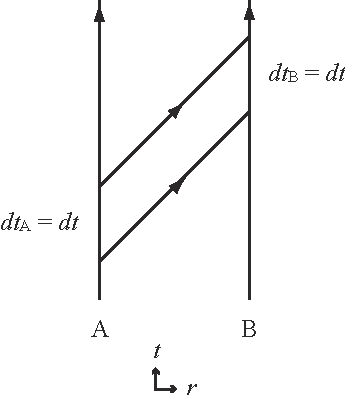
\includegraphics{Ch2_red_shift.pdf} }
\vskip2mm
\caption{Exchange of light between A and B.
%A��B�̌��̂��Ƃ�D
}
\label{fig:red_shift}
\end{center}
\end{figure}%
%%============

The  \keyword{gravitational redshift} is one of three ``classic tests" of general relativity; the other two are mentioned in \sect{geodesics_flat}.
% added
The discussion here is used to discuss the surface gravity (\sect{surface_grav}) and to discuss the gravitational redshift in the AdS spacetime (\sect{geodesics_AdS}).
%{\bf �d�͐ԕ��Έ�}\index{���䂤��悭�����ق��ւ�@�d�͐ԕ��Έ�}�́C��ʑ��Θ_�̌ÓT�I�\���ƌĂ΂��3�‚̗\����1�‚ł���D�i�ق���2�‚ɂ‚��Ă�\sect{geodesics_flat}�łӂ��j

Consider two static observers at A and B (\fig{red_shift}). The observer at A sends light, and the observer at B receives light. The light follows the null geodesics $ds^2=0$, so
%�n�_A��B�ɁC���ꂼ��Î~�����ϑ��҂�����Ƃ���DA�Ŕ����������CB�Ŏ󂯂Ƃ���̂Ƃ���D����$p^2=0$ ���邢�̓k�����n�� $ds^2=0$��`���̂ŁC
\begin{align}
%
ds^2 &= g_{00} dt^2+ g_{rr} dr^2 = 0~, \\
dt^2 &= \frac{g_{rr}}{-g_{00}} dr^2 
\result
\int_A^B dt = \int_A^B \sqrt{ \frac{g_{rr}(r)}{-g_{00}(r)} } dr~.
%\label{eq:}
%
\end{align}
The right-hand side of the final expression does not depend on when light is sent, so the coordinate time until light reaches from A to B is always the same. Thus, if the observer at A emits light for the interval $dt$, the observer at B receives light for the interval $dt$ as well.
%�E�ӂ͎����Ɉˑ����Ȃ��̂ŁC����A����B�ɓ��B����̂ɂ�������W���Ԃ͏�ɓ����ł���D���������āCA��$dt$�̂������������𔭂����Ƃ���ƁCB�����̌����󂯂Ƃ�̂ɂ�������W���Ԃ�$dt$ �ł���i\fig{red_shift}�j�D

However, the proper time for each observer differs since $d\tau^2 = |g_{00}| dt^2$:
%�������C $d\tau^2 = |g_{00}| dt^2$ �Ȃ̂ŁC���ꂼ��̊ϑ��҂ɂƂ��Ă̌ŗL���Ԃ̐i�݂͈Ⴄ�F
\begin{align}
%
d\tau_A^2 &\simeq |g_{00}(A)| dt^2~, \\
d\tau_B^2 &\simeq |g_{00}(B)| dt^2~.
%\label{eq:}
%
\end{align}
But both observers should agree to the total number of light oscillations, so
%�ǂ���̊ϑ��҂ɂƂ��Ă��C���̑��U�����͓����͂�������C
\be
%
\omega_B d\tau_B = \omega_A d\tau_A~.
%
\ee
The energy of the photon is given by $E=\hbar \omega$, so $ E_B d\tau_B = E_A d\tau_A $, or 
%���q�̃G�l���M�[��$E=\hbar \omega$�Ȃ̂ŁC$ E_B d\tau_B = E_A d\tau_A $ �‚܂�
\be
%
\boxeq{
\frac{E_B}{E_A} =\sqrt{\frac{g_{00}(A)}{g_{00}(B)}}~.
}
\label{eq:red_shift}
%
\ee

For simplicity, consider the Schwarzschild black hole and set $r_B=\infty$ and $r_A \gg GM$. Then,
%�ȒP�ȏꍇ�Ƃ��ăV�������c�V���h�E�u���b�N�z�[�����l���C $r_B=\infty, r_A \gg GM$�Ƃ���ƁC
\be
%
% 2015/3/30: corrected
E_\infty = \sqrt{|g_{00}(A)|} E_A
\simeq E_A - \frac{GM}{r_A} E_A < E_A~.
\label{eq:red_shift_int}
%
\ee
Here, we used $\sqrt{|g_{00}(A)|} = (1-2GM/r_A)^{1/2} \simeq 1-(GM)/r_A$. Thus, the energy of the photon decreases at infinity. The energy of the photon decreases because the photon has to climb up the gravitational potential. Indeed, the second term of \eq{red_shift_int} takes the form of the Newtonian potential for the photon. Also, suppose that the point A is located at the horizon. Since $g_{00}(A)=0$ at the horizon, $E_\infty\rightarrow0$, namely light gets an infinite redshift.
%�����ŁC$\sqrt{|g_{00}(A)|} = (1-2GM/r_A)^{1/2} \simeq 1-(GM)/r_A$���g�����D���������āC�������ł̌��q�̃G�l���M�[�͌�������D�Ƃ���A���z���C�Y���̏ꍇ�C$g_{00}(A)=0$�Ȃ̂ŁC$E_\infty\rightarrow0$�ƂȂ��āC���q�͖����̐ԕ��Έڂ��󂯂�D���q�̃G�l���M�[����������̂́C�d�̓|�e���V�������オ�������߂ł���D���ہC\eq{red_shift_int}�̑�2���͌��q�ɑ΂���j���[�g���I�ȏd�̓|�e���V�����̌`�����Ă���D


%%------------------
\subsection{Particle motion
%���q�̉^��
}\label{sec:geodesics}
%%------------------

%%------------------
\subsubsection*{Motion far away
%�����ł̉^��
}\label{sec:geodesics_flat}
%%------------------

The particle motion can be determined from the geodesic equation \eqref{eq:geodesic_eq}. However, there are enough number of conserved quantities for a static spherically symmetric solution such as the Schwarzschild black hole, which completely determines the particle motion without solving the geodesic equation.
%���q�̉^���͑��n�������� \eqref{eq:geodesic_eq} ���狁�߂��邪�C�V�������c�V���h�E�u���b�N�z�[���̂悤�ȐÓI���Ώ̉��̏ꍇ�C���n���������������܂ł��Ȃ��ۑ������狁�߂邱�Ƃ��ł���D
\begin{itemize}

\item
First, because  of spherical symmetry, the motion is restricted to a single plane, and one can choose the equatorial plane ($\theta=\pi/2$) as the plane without loss of generality. 
%�܂����Ώ̂̏ꍇ�C�^���͂P�‚̕��ʓ��Ɍ��肳���̂ŁC���̕��ʂ�ԓ��ʁi$\theta=\pi/2$�j�ɑI�ׂ�D

\item
Second, as we saw in \sect{particle_action_curved}, when the metric is independent of a coordinate $x^\mu$, its conjugate momentum $p_\mu$ is conserved. For a static spherically symmetric solution, the metric is independent of  $t$ and $\varphi$, so the energy  $p_0$ and the angular momentum  $p_\varphi$ are conserved. 
%�܂��C\sect{particle_action_curved}�ł݂��Ƃ���C�v�ʂ��C������W$x^\mu$���܂܂Ȃ��ꍇ�C$x^\mu$�ɋ����ȉ^����$p_\mu$���ۑ�����D�ÓI���Ώ̉��̏ꍇ�C�v�ʂ� $t$, $\varphi$ �ɂ��Ȃ����߁C�G�l���M�[ $p_0$�C�p�^���� $p_\varphi$ ���ۑ�����D
\end{itemize}
Then, the particle four-momentum is given by
%���������āC���q��4���^���ʂ�
%\begin{subequations}
\begin{align}
%
p_0 &=: -mE~, \\
p_\varphi &=: mL~, \\
p^r &= m \frac{dr}{d\tau}~, \\
p^\theta &=0~.
%\label{eq:}
%
\end{align}
%\end{subequations}
($E$ and $L$ are the energy and the angular momentum per unit rest mass.) Because the four-momentum satisfies the constraint $p^2=-m^2$, 
%�i$E, L$ �͒P�ʎ��ʂ�����̃G�l���M�[�Ɗp�^���ʁj�D�^���ʂ͍S������ $p^2=-m^2$ �𖞂����̂�
\be
%
g^{00}(p_0)^2 + m^2 g_{rr} \left(\frac{dr}{d\tau}\right)^2 + g^{\varphi\varphi}(p_\varphi)^2 = -m^2~.
\label{eq:constraint_on_shell1}
%
\ee
Substitute the metric of the Schwarzschild black hole. When the angular momentum $L=0$, 
%�V�������c�V���h�E�u���b�N�z�[���ł́C�܂��p�^���� $L=0$ �̂Ƃ���
\be
%
\left(\frac{dr}{d\tau}\right)^2 
= (E^2 - 1) + \frac{2GM}{r}~.
\label{eq:massive_noL}
%
\ee
Since $(dr/d\tau)^2 \simeq E^2 - 1$ as $r\rightarrow\infty$, $E=1$ represents the energy when the particle is at rest at infinity, namely the rest mass energy of the particle. Differentiating this equation with respect to $\tau$ and using $\tau \simeq t$ in the nonrelativistic limit, one gets
%$r\rightarrow\infty$ �� $(dr/d\tau)^2 \simeq E^2 - 1$ �Ȃ̂ŁC$E=1$ �͖��������ŗ��q���Î~��Ԃɂ������ꍇ�̃G�l���M�[�C�‚܂藱�q�̎��ʃG�l���M�[������킷�D���̎��� $\tau$ �Ŕ������C�񑊑Θ_�I�ȏꍇ�� $\tau \simeq t$ �ƂȂ�̂�
\be
%
\frac{d^2r}{dt^2} \simeq - \frac{GM}{r^2}~,
%
\ee
which is nothing but the Newton's law of gravitation. Thus, $M$ in the Schwarzschild black hole \eqref{eq:Schwarzschild} represents the black hole mass.
%����̓j���[�g���̏d�͖@���ɂق��Ȃ�Ȃ��D���������āC�V�������c�V���h�E�u���b�N�z�[�� \eqref{eq:Schwarzschild} �� $M$ �̓u���b�N�z�[���̎��ʂ�����킷�D

Similarly, when $L \neq 0$,
%���l�Ɋp�^���� $L$ ������ꍇ�C
\begin{align}
%
\left(\frac{dr}{d\tau}\right)^2 
&= E^2 - \left( 1-\frac{2GM}{r} \right)\left( 1+\frac{L^2}{r^2} \right) \\
&=  (E^2 - 1) + \frac{2GM}{r} - \frac{L^2}{r^2} + \frac{2GML^2}{r^3}~.
\label{eq:massive_L}
%\label{eq:}
%
\end{align}
The third term in \eq{massive_L} represents the centrifugal force term. On the other hand, the fourth term is a new term characteristic of general relativity. General relativity has ``classic tests" such as 
%\eq{massive_L}�̑�3���͉��S�͂�����킷�D����ɑ΂��āC��4���͐V�������ł���C��ʑ��Θ_�I�Ȍ��ʂ�����킷�D��ʑ��Θ_�̌ÓT�I�\���ɂ́C�d�͐ԕ��ΈڈȊO��
\begin{itemize}
\item The perihelion shift of Mercury %�����̋ߓ��_�ړ�
\item The light bending %���̋Ȃ���
\end{itemize}
in addition to the gravitational redshift, and both effects come from this fourth term%
\footnote{For the light bending, use the equation for the massless particle instead of \eq{constraint_on_shell1}. }.
The fourth term is comparable to the third term only when the particle approaches $r \simeq 2GM$. This distance corresponds to the horizon radius of the black hole and is about 3km for a solar mass black hole, so the effect of this term is normally very small.
%�����邪�C����������̍�����̌��ʂł���%
%\footnote{���̋Ȃ���̏ꍇ�́C\eq{constraint_on_shell1} �̂����Ɏ��ʃ[���̎����g���D}�D
%��3���Ƒ�4�����ׂ�ƁC��4���� $r \simeq 2GM$ ���x�ɋ߂Â��Ă͂��߂đ�3���Ɠ����̊�^�ƂȂ�D���̋����̓u���b�N�z�[���̃z���C�Y�����a�ɑ������C���z���ʂ̏d�͏�̏ꍇ�C3km���x�Ȃ̂ŁC�ʏ����Ȍ��ʂ��Ƃ������Ƃ��킩��D

% added
We will generalize the discussion here to a generic static metric in order to discuss the surface gravity in \sect{surface_grav}. We will also examine the particle motion in the AdS spacetime in \sect{geodesics_AdS}.

%%------------------
\subsubsection*{Motion near horizon
%�z���C�Y���ߖT�ł̉^��
}\label{sec:geodesics_horizon}
%%------------------

We now turn to the particle motion near the horizon. How long does it take until the particle reaches the horizon? For simplicity, we assume that the particle is at rest at infinity ($E=1$) and that the particle falls radially ($L=0$). From \eq{massive_noL}, the particle motion for $E=1$ and $L=0$ is given by
%���ɁC�z���C�Y���ߖT�ł̗��q�̉^�����l����D�z���C�Y���ɗ�������܂ł̎��Ԃ����߂�D�ȒP�̂��߂ɁC�������ł͐Î~��Ԃɂ���i$E=1$�j�C���a�����ɂ܂�����������^���i$L=0$�j���l����D$E=1, L=0$ �̗��q�̉^���́C\eq{massive_noL} ���
\be
%
\left(\frac{dr}{d\tau}\right)^2 
= \frac{r_0}{r}
%\label{eq:}
%
\ee
($r_0=2GM$). Near the horizon,
%�i$r_0=2GM$�j�D�z���C�Y���ߖT�ł�
\be
%
\frac{dr}{d\tau} \simeq -1~.
%\label{eq:}
%
\ee
We choose the minus sign since the particle falls inward ($r$ decreases as time passes). So, to go from $r=r_0+R$ to $r=r_0+\epsilon$,
%�ƂȂ�D�������闱�q�ɑ΂��ẮC���Ԍo�߂ƂƂ���$r$���������Ȃ�̂ŁC�E�ӂ̕����𕉂ɑI�񂾁D���������āC $r=r_0+R$ ���� $r=r_0+\epsilon$ �܂œ����̂�
\be
%
\tau \simeq -\int_{r_0+R}^{r_0+\epsilon} dr = R - \epsilon~.
%\label{eq:}
%
\ee
Namely, the particle reaches the horizon in a \textit{finite proper time.}
%���Ȃ킿�C�������闱�q�̌ŗL����$\tau$�̗���ł́C{\bf �L�����ԂŃz���C�Y���ɓ��B����D}

However, the story changes from the point of view of the coordinate time $t$. By definition, $p^0 = mdt/d\tau$, and from the conservation law, $p^0 = g^{00}p_0 = m(1-r_0/r)^{-1}$. Then,
%����C���W����$t$�̗���ł́C�b���ς���Ă���D��`��� $p^0 = mdt/d\tau$ �����C����ۑ������ $p^0 = g^{00}p_0 = m(1-r_0/r)^{-1}$ �Ȃ̂ŁC
\be
%
\frac{d\tau}{dt} = \frac{r-r_0}{r}~.
%\label{eq:}
%
\ee
Thus,
\be
%
\left(\frac{dr}{dt}\right)^2 
= \left(\frac{dr}{d\tau}\right)^2 \left(\frac{d\tau}{dt}\right)^2 
= \frac{r_0(r-r_0)^2}{r^3}
%\label{eq:}
%
\ee
or
%�z���C�Y���ߖT�ł�
\be
%
\frac{dr}{dt} \simeq - \frac{r-r_0}{r_0}
\label{eq:timelike_horizon_t}
%
\ee
near the horizon, and
%�Ȃ̂ŁC
\be
%
t \simeq - r_0 \int_{r_0+R}^{r_0+\epsilon} \frac{dr}{r-r_0} = r_0(\ln R - \ln \epsilon)~,
%\label{eq:}
%
\ee
so $t\rightarrow\infty$ as $\epsilon\rightarrow0$. Namely, it takes an \textit{infinite coordinate time} until the particle reaches the horizon. Incidentally, \eq{timelike_horizon_t} near the horizon takes the same form as the massless case below. Namely, the particle moves with the speed of light near the horizon.
%$\epsilon\rightarrow0$��$t\rightarrow\infty$�ƂȂ�̂ŁC$t$�̗���ł́C{\bf ���q���z���C�Y���ɓ��B����̂ɖ����̎��Ԃ�������D} �Ȃ��C�z���C�Y���ߖT��\eq{timelike_horizon_t}�͌��q \eqref{eq:null_horizon_t} �Ɠ����`�ɂȂ�D�‚܂�z���C�Y���ߖT�ł́C���q�̑��x�͌����ɋ߂Â��D

Let us consider the massless case. For the massless particle, $p^2=0$ or $ds^2=0$, so
%���q�̏ꍇ���l���Ă݂悤�D���q�ɑ΂��ẮC$p^2=0$ ���邢�� $ds^2=0$ �Ȃ̂ŁC
%\begin{subequations}
%\label{eq:}
\begin{align}
%
& ds^2 = g_{00} dt^2+ g_{rr} dr^2 = 0
\\
&\rightarrow 
\left(\frac{dr}{dt}\right)^2 
= - \frac{ g_{00} }{ g_{rr} }
= \left( 1-\frac{r_0}{r} \right)^2 
\\
&\rightarrow
\frac{dr}{dt} = - \left( 1-\frac{r_0}{r} \right) \simeq - \frac{r-r_0}{r_0}~.
\label{eq:null_horizon_t}
%\label{eq:}
%
\end{align}
%\end{subequations}
Near the horizon, the expression takes the same form as the massive case  \eqref{eq:timelike_horizon_t} as promised. We considered the infalling photon, but one can consider the outgoing photon. In this case, $t\rightarrow\infty$ until the light from the horizon reaches the observer at finite $r$.
%���������āC�z���C�Y���ߖT�ł͗��q�̏ꍇ \eqref{eq:timelike_horizon_t} �Ɠ����`�ł���D�܂��C���q���z���C�Y���ɗ�������ꍇ�ł͂Ȃ��C�t�Ɍ��q���z���C�Y������O�����ɏo��ꍇ��z�肷��ƁC�z���C�Y���ŏo�������i�L��$r$�ł��j�ϑ��҂ɓ��B����̂�$t\rightarrow\infty$�ł���D

There is nothing special to the horizon from the point of view of the infalling particle. But there is a singular behavior from the point of view of the coordinate $t$. This is because the Schwarzschild coordinates $(t,r)$ are not well-behaved near the horizon. Thus, we introduce the coordinate system which is easier to see the infalling particle point of view.
%�������闱�q�̗���ł́C�z���C�Y���œ���Ȃ��Ƃ͂Ȃ��̂ɑ΂��C$t$�̗���ł͓��قȂ��Ƃ��N���Ă���D����̓z���C�Y���ߖT�ł̓V�������c�V���h���W$(t,r)$�̐U��܂����������Ƃ��Ӗ����Ă���D�����ŁC�������闱�q�̗��ꂪ�݂₷�����W�n�𓱓����邱�Ƃɂ���D


%%%%%%%%%
\section{Kruskal coordinates%�N���X�J�����W
}%\label{sec:}
%%%%%%%%%

%%============
\begin{figure}[tb]
\centering
%\hspace{0.25in}
\scalebox{0.75}{ 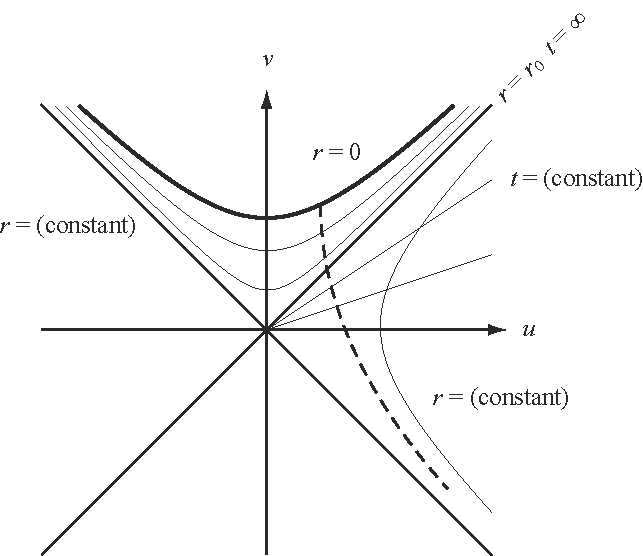
\includegraphics{Ch2_kruskal.pdf} }
\vskip2mm
\caption{Kruskal coordinates. The light-cones are kept at 45$^\circ$, which is convenient to see the causal structure. The dashed line represents an example of the particle path. Once the particle crosses the horizon, it must reach the singularity.
%�N���X�J�����W�D���~����45���ɕۂ���C���ʍ\�������₷���D�������͓��ٓ_������킷�D�j���͗��q�̋O�Ղ̈��ł���D�z���C�Y�������؂�ƁC���q�͓��ٓ_�ɓ��B����������Ȃ��D
}
\label{fig:kruskal}
\end{figure}%
%%============

The particle motion discussed so far can be naturally understood by using a new coordinate system, the \keyword{Kruskal coordinates}. The Kruskal coordinates $(u,v)$ are defined by
%����܂łɂ킩�������q�̉^���́C�V�������W�n�C{\bf �N���X�J��}�iKruskal�j{\bf ���W}\index{���邷���邳�Ђ悤@�N���X�J�����W}�𓱓����邱�ƂŎ��R�ɗ����ł���D�N���X�J�����W $(u,v)$ ��
\begin{align}
%
r>r_0 & \left\{
\begin{array}{l}
  u = \left( \frac{r}{r_0}-1 \right)^{1/2} e^{r/(2r_0)} \cosh \left(\frac{t}{2r_0}\right) \\
  v = \left( \frac{r}{r_0}-1 \right)^{1/2} e^{r/(2r_0)} \sinh \left(\frac{t}{2r_0}\right)
\end{array}
\right. 
\label{eq:kruskal} \\
r<r_0 & \left\{
\begin{array}{l}
  u = \left( 1-\frac{r}{r_0} \right)^{1/2} e^{r/(2r_0)} \sinh \left(\frac{t}{2r_0}\right) \\
  v = \left( 1-\frac{r}{r_0} \right)^{1/2} e^{r/(2r_0)} \cosh \left(\frac{t}{2r_0}\right)
\end{array}
\right.
%\label{eq:}
%
\end{align}
By the coordinate transformation, the metric \eqref{eq:Schwarzschild} becomes
%�Ƃ��Ē�`�����D�v�� \eqref{eq:Schwarzschild} �����W�ϊ�����ƁC
\be
%
ds^2 = \frac{4r_0^3}{r} e^{-r/r_0} ( -dv^2+du^2 ) + r^2 d\Omega_{2}^2~.
\label{eq:metric_kruskal}
%
\ee
Here, we use not only $(u,v)$ but also use $r$, but $r$ should be regarded as $r=r(u,v)$ and is determined by
%��̌v�ʂł� $(u,v)$ �����ł͂Ȃ� $r$ ���p���Ă��邪�C$r=r(u,v)$ �ł���C
\be
%
\left( \frac{r}{r_0}-1 \right) e^{r/r_0} = u^2-v^2~.
\label{eq:r&uv}
%
\ee
%���猈�܂�D

One can see the following various properties from the coordinate transformation and the metric (see also \fig{kruskal}):
%���̕ϊ��ƌv�ʂ���C�ȉ��̂��܂��܂Ȃ��Ƃ��킩��i\fig{kruskal}���Q�Ɓj�F
\begin{itemize}

\item
The metric \eqref{eq:metric_kruskal} is not singular at $r=r_0$. There is a singularity at $r=0$. The transformation \eqref{eq:kruskal} is singular at $r=r_0$, but this is not a problem. Because the transformation relates the coordinates which are singular at $r=r_0$ to the coordinates which are not singular at $r=r_0$, the transformation should be singular there. 
%$r=r_0$ �Ōv�� \eqref{eq:metric_kruskal} �ɓ��ِ��͂Ȃ��D$r=0$�ɂ͓��ِ����c��D�ϊ� \eqref{eq:kruskal} �ɂ�$r=r_0$�œ��ِ������邪�C����͖��ɂ͂Ȃ�Ȃ��D$r=r_0$�œ��ِ���������W�Ɠ��ِ����Ȃ����W��ϊ�����̂ŁC���̓��ِ��͓��R�ł���D

\item
The null world-line $ds^2=0$ is given by $dv=\pm du$. In this coordinate system, the lines at 45$^\circ$ give light-cones just like special relativity, which is convenient to see the causal structure of the spacetime. 
%�k�����E�� $ds^2=0$ �� $dv=\pm du$ �ł���D���̍��W�n�ł́C���ꑊ�Θ_�̂悤��45���̐������~��������킷�D���̂��߈��ʍ\�������₷�����_������D

\item
The $r=\text{(constant)}$ lines are hyperbolas from \eq{r&uv}. 
%\eq{r&uv} ���$r=\text{(constant)}$�̐��́C�o�Ȑ��ł���D

\item
% added
In particular, in the limit $r=r_0$, the hyperbola becomes a null line, so \textit{the horizon $r=r_0$ is a null surface}. Namely, the horizon is not really a spatial boundary but is a light-cone. In special relativity, the events inside light-cones cannot influence the events outside light-cones. Similarly, the events inside the horizon cannot influence the events outside the horizon. Then, even light cannot reach from $r<r_0$ to $r>r_0$.
%�Ƃ��ɁC$r=r_0$��{\bf �z���C�Y���́C�k�����E�ʂł���D}�‚܂�C�z���C�Y���͎��ۂɂ͋�Ԃ̋��E������킵�Ă���̂ł͂Ȃ��C���~�����̂��̂ł���D���~���̓�����O�ւ͉e�����y�ڂ����Ƃ��ł��Ȃ��D���l�ɁC�z���C�Y�����z���C�Y���̊O�ւ͉e�����y�ڂ����Ƃ��ł��Ȃ��D�‚܂�C��������$r<r_0$����$r>r_0$�ɂ͓͂��Ȃ��D

\item
For $r<r_0$, the $r=\text{(constant)}$ lines become spacelike. This means that a particle cannot remain at $r=\text{(constant)}$ because the geodesics of a particle cannot be spacelike. The singularity at $r=0$ is spacelike as well. Namely, the singularity is not a point in spacetime, but rather it is the end of ``time."
%$r<r_0$�ł́C$r=\text{(constant)}$�̐��͋�ԓI�ɂȂ�D���q�̑��n���͋�ԓI�ɂ͂Ȃ�Ȃ��̂ŁC���q��$r=\text{(constant)}$�ɂ͂Ƃǂ܂�Ȃ��D$r=0$�̓��ٓ_����ԓI�ł���D�‚܂�C���ٓ_�͋�Ԃ̈�_�ł͂Ȃ��C�ނ��뎞�Ԃ̏I���Ƃ����Ӗ������D

\item
The $t=\text{(constant)}$ lines are straight lines. In particular, the $t \rightarrow\infty$ limit is given by $u=v$. One can see that it takes an infinite coordinate time to reach the horizon.
%\eq{kruskal} ���$t=\text{(constant)}$�̐��́C�����ł���D�Ƃ��ɁC$t \rightarrow\infty$��$u=v$�ł���D���W$t$�ł́C�z���C�Y���ɓ��B����̂ɖ����̎��Ԃ�������̂��ǂ݂Ƃ��D

\end{itemize}
To summarize, the particle falling into the horizon cannot escape and necessarily reaches the singularity.
%�����̂��Ƃ��܂Ƃ߂�ƁC�z���C�Y���ɗ��������q�͓����ꂸ�C�K�R�I�ɓ��ٓ_�ɓ��B���邱�ƂɂȂ�D

%%------------------
\titlenewterms%
%%------------------

After you read each chapter, try to explain the terms in ``New keywords" by yourself to check your understanding.

\begin{multicols}{2}
\noindent
horizon\\
proper time\\
world-line\\
four-velocity\\
geodesic\\
%geodesic equation\\
affine parameter\\
cosmological constant\\
Schwarzschild black hole\\
spacetime singularity\\
gravitational redshift\\
Kruskal coordinates\\
\end{multicols}

%%%%%%%%%
%\section*{Appendix: Review of general relativity}
%\addcontentsline{toc}{section}{Appendix: Review of general relativity}\label{sec:GR}
\section{Appendix: Review of general relativity
%���F��ʑ��Θ_�̂����炢
}\label{sec:GR}
%%%%%%%%%

Consider a coordinate transformation
%��ʍ��W�ϊ�
\be
%
x'^\mu = x'^\mu (x)~.
%\label{eq:}
%
\ee
Under a coordinate transformation, a quantity is called a vector if it transforms as
%�̉��ŁC
\be
%
V'^\mu= \frac{\del x'^\mu}{\del x^\nu} V^\nu~,
%\label{eq:}
%
\ee
and as a 1-form if it transforms ``oppositely": 
%�ƕϊ�����ʂ��x�N�g���C�u�t�v�̕ϊ���
\be
%
V'_\mu= \frac{\del x^\nu}{\del x'^\mu} V_\nu~.
%\label{eq:}
%
\ee
The tensors with a multiple number of indices are defined similarly.
%�����—ʂ�1�t�H�[���ƌ����D�Y���𕡐����ƒe���\�������l�ɒ�`����D

In general, the derivative of a tensor such as  $\del_\mu V^\nu$ does not transform as a tensor, but the covariant derivative $\nabla_\mu$ of a tensor transforms as a tensor. The covariant derivatives of the vector and the 1-form are given by
%��ʂɃe���\���̔��� $\del_\mu V^\nu$ �́C�e���\���Ƃ��ĕϊ����Ȃ��D�����ŁC�e���\���Ƃ��ĕϊ����鋤�ϔ��� $\nabla_\mu$ ���g���D�x�N�g����1�t�H�[���̏ꍇ�C���ϔ�����
\begin{align}
%
\nabla_\mu V^\nu &= \del_\mu V^\nu + V^\alpha \Gamma^\nu_{~\alpha\mu}~, \\
\nabla_\mu V_\nu &= \del_\mu V_\nu - V_\alpha \Gamma^\alpha_{~\mu\nu}~.
%\label{eq:}
%
\end{align}
As a useful relation, the covariant divergence of a vector is given by
%�܂��C�L�p�Ȋ֌W���Ƃ��āC�x�N�g���̔��U��
\be
%
\nabla_\mu V^\mu = \frac{1}{\sqrt{-g}} \del_\mu \left(\sqrt{-g} V^\mu \right)~,
%\label{eq:}
%
\ee
% added
where $g:= \det g$. This can be shown using a formula for a matrix $M$:
\be
%
\del_\mu(\det M) = \det M\, \text{tr}(M^{-1}\del_\mu M)~.
\label{eq:matrix_formula}
%
\ee

For example, $dx^\mu$ transforms as a vector 
%��Ƃ��āC
\be
%
dx'^\mu= \frac{\del x'^\mu}{\del x^\nu} dx^\nu
\label{eq:dx_transf}
%
\ee
and the metric transforms as
%�̓x�N�g���Ƃ��ĕϊ����C�v�ʂ�
\be
%
g'_{\mu\nu}(x') = \frac{\del x^\rho}{\del x'^\mu}  \frac{\del x^\sigma}{\del x'^\nu}  g_{\rho\sigma}(x)~.
\label{eq:metric_transf}
%
\ee
Thus, the line element $ds^2 = g_{\mu\nu}dx^\mu dx^\nu$ is invariant under coordinate transformations. Under the infinitesimal transformation $x'^\mu = x^\mu - \xi^\mu(x)$, \eq{metric_transf} is rewritten as
%�ƕϊ�����D���������āC���f $ds^2 = g_{\mu\nu}dx^\mu dx^\nu$ �͍��W�ϊ��̉��ŕs�ςł���D�������ϊ� $x'^\mu = x^\mu - \xi^\mu(x)$ �̉��ŁC\eq{metric_transf} ������������ƁC
\be
%
g'_{\mu\nu} (x-\xi) = 
\left(\delta^\rho_{~\mu} + \del_\mu\xi^\rho \right)
\left(\delta^\sigma_{~\nu} + \del_\nu\xi^\sigma \right)g_{\rho\sigma}
%\label{eq:}
%
\ee
or
%���
\begin{align}
%
g'_{\mu\nu} (x) &= 
g_{\mu\nu}(x) + (\del_\mu\xi^\rho) g_{\rho\nu} + (\del_\nu\xi^\rho) g_{\mu\rho} 
+ \xi^\rho \del_\rho g_{\mu\nu} \\
&= g_{\mu\nu} + \nabla_\mu\xi_\nu +  \nabla_\nu\xi_\mu~.
\label{eq:metric_transf_inf}
%\label{eq:}
%
\end{align}
%�ƂȂ�D

In general relativity, an action must be a scalar which is invariant under coordinate transformations. From \eq{dx_transf},
%��ʑ��Θ_�ł́C��p�͈�ʍ��W�ϊ��̉��ŕs�ςȃX�J���[�ʂł��邱�Ƃ�v������D\eq{dx_transf} ���C
\be
%
d^{4}x' = \left| \frac{\del x'}{\del x} \right| d^{4}x~,
%\label{eq:}
%
\ee
where $| \del x'/\del x |$ is the Jacobian of the transformation. On the other hand, $\sqrt{-g}$ transforms in the opposite manner: 
%$| \del x'/\del x |$ �̓��R�r�A���ł���D����C
\be
%
\sqrt{-g'} = \left| \frac{\del x}{\del x'} \right| \sqrt{-g}~. 
%\label{eq:}
%
\ee
Thus, $d^{4}x\, \sqrt{-g}$ is the volume element which is invariant under coordinate transformations.
%�ƂȂ�̂ŁC��ʍ��W�s�ςȑ̐ϗv�f�� $d^{4}x\, \sqrt{-g}$ �ł���D

The metric is determined by the Einstein-Hilbert action:
%�v�ʂ̓A�C���V���^�C��-�q���x���g��p�ɂ���Č��܂�F
\be
%
\action = \frac{1}{16\pi G} \int d^{4}x\, \sqrt{-g} R~.
%\label{eq:}
%
\ee
Here, $G$ is the Newton's constant, and the Ricci scalar $R$ is defined by the Riemann tensor $R^\alpha_{~\mu\nu\rho}$ and the Ricci tensor $R_{\mu\nu}$ as follows:
%������ $G$ �̓j���[�g���萔�ł���C���b�`�E�X�J���[ $R$ �́C���[�}���e���\�� $R^\alpha_{~\mu\nu\rho}$�C���b�`�E�e���\�� $R_{\mu\nu}$ ����ȉ��̂悤�ɒ�`�����F 
\begin{align}
%
R^\alpha_{~\mu\nu\rho} &=
\del_\nu \Gamma^\alpha_{~\mu\rho} - \del_\rho \Gamma^\alpha_{~\mu\nu}
+ \Gamma^\alpha_{~\sigma\nu}\Gamma^\sigma_{~\mu\rho}
- \Gamma^\alpha_{~\sigma\rho}\Gamma^\sigma_{~\mu\nu}~, \\
%
R_{\mu\nu} &= R^\alpha_{~\mu\alpha\nu}~, \quad
R = g^{\mu\nu} R_{\mu\nu}~.
%\label{eq:}
%
\end{align}
The variation of the Einstein-Hilbert action gives 
%�A�C���V���^�C��-�q���x���g��p��ϕ�����ƁC
\begin{align}
%
\delta \action &= \frac{1}{16\pi G} \int d^{4}x\, 
\left\{
\sqrt{-g} R_{\mu\nu} (\delta g^{\mu\nu}) + (\delta\sqrt{-g}) R_{\mu\nu}g^{\mu\nu} \right. 
\nonumber \\
& \left. \hspace{2cm} + \sqrt{-g} (\delta R_{\mu\nu}) g^{\mu\nu} 
\right\}~,
%\label{eq:}
%
\end{align}
where $g^{\mu\nu}$ is the inverse of $g_{\mu\nu}$. The second term can be rewritten by using%
% added
\footnote{Using \eq{matrix_formula} gives $\delta(\sqrt{-g}) = \frac{1}{2} \sqrt{-g} g^{\mu\nu} \delta g_{\mu\nu}$. Then, use another matrix formula $\delta M = -M \delta (M^{-1}) M$ which can be derived from $MM^{-1}=I$. Then, $ \delta g_{\mu\nu} = -g_{\mu\rho} g_{\nu\sigma}\delta g^{\rho\sigma}$. Note that $ \delta g_{\mu\nu} \neq g_{\mu\rho} g_{\nu\sigma}\delta g^{\rho\sigma}$. Namely, we do not use the metric to raise and lower indices of the metric variation.}
%$g^{\mu\nu}$��$g_{\mu\nu}$�̋t�s��ł���D��2���ڂ�
\be
%
\delta \sqrt{-g} = - \frac{1}{2} \sqrt{-g} g_{\mu\nu} \delta g^{\mu\nu}~.
%\label{eq:}
%
\ee
One can show that the third term reduces to a surface term, so it does not contribute to the equation of motion%
\footnote{Care is necessary to the surface term in order to have a well-defined variational principle. This issue will be discussed in Sects.~\ref{sec:SAdS_free} and \ref{sec:action_tensor}.}. 
Therefore,
%���g���D��3���ڂ́C�\�ʍ��ɋA�����邱�Ƃ��������Ƃ��ł���̂ŁC�^���������ɂ͊�^���Ȃ�%
%\footnote{�������C�ϕ������� well-defined �ɂ����Ȃ����߂ɁC�\�ʍ��ɂ͓��ʂȒ��ӂ��K�v�ł���D���̓_�ɂ‚��Ċ֘A���鎖���\ref{sec:SAdS_free}�C\ref{sec:action_tensor}~�߂łӂ��D}�D���������āC
\be
%
\delta \action = \frac{1}{16\pi G} \int d^{4}x\, \sqrt{-g} 
\left(R_{\mu\nu} -\frac{1}{2} g_{\mu\nu} R \right) \delta g^{\mu\nu}~,
%\label{eq:}
%
\ee
and by requiring $\delta \action=0$, one gets the vacuum Einstein equation:
%�ƂȂ�C$\delta \action=0$ ��v�����Đ^�󒆂̃A�C���V���^�C����������������F
\be
%
R_{\mu\nu} - \frac{1}{2} g_{\mu\nu} R = 0~.
\label{eq:Einstein_vac_again}
%
\ee
The contraction of \eq{Einstein_vac_again} gives $R_{\mu\nu}=0$.
%\eq{Einstein_vac_again} �̏k����Ƃ�ƁC$R_{\mu\nu}=0$ �ƂȂ�D

When one adds the matter action $\action_\text{matter}$, the equation of motion becomes
%������̍�p $\action_\text{matter}$ ��������ƁC�^����������
\be
%
R_{\mu\nu} - \frac{1}{2} g_{\mu\nu} R = 8\pi G\, T_{\mu\nu}~,
%\label{eq:}
%
\ee
where $T_{\mu\nu}$ is the energy-momentum tensor for matter fields:
%������ $T_{\mu\nu}$ �́C������̃G�l���M�[�E�^���ʃe���\���ł���F
\be
%
T_{\mu\nu} := - \frac{2}{\sqrt{-g}} \frac{\delta \action_\text{matter}}{\delta g^{\mu\nu}}~.
\label{eq:EM_tensor}
%
\ee
Various matter fields appear in this book, but the simplest term one can add to the Einstein-Hilbert action is given by
%�{���ł͂��܂��܂ȕ����ꂪ�o�ꂷ�邪�C�A�C���V���^�C��-�q���x���g��p�ɉ����邱�Ƃ��ł�������Ƃ��P���ȍ�p�́C
\be
%
\action_{cc} = -\frac{1}{8\pi G} \int d^{4}x\, \sqrt{-g} \Lambda~,
%\label{eq:}
%
\ee
which is the cosmological constant term. From \eq{EM_tensor},
%�ł���C���ꂪ�F���萔�ł���D\eq{EM_tensor} ���C
\be
%
T_{\mu\nu} = - \frac{\Lambda}{8\pi G} g_{\mu\nu}~,
\label{eq:EM_tensor_cc_again}
%
\ee
so the Einstein equation becomes
%�ł���C�A�C���V���^�C����������
\be
%
R_{\mu\nu} - \frac{1}{2} g_{\mu\nu} R + \Lambda g_{\mu\nu} = 0~.
%\label{eq:}
%
\ee
%�ƂȂ�D

\endofsection

	%\documentclass[11pt]{jarticle} %%% �A���R�����g
\ifx\nameofpaper\undefined %%% ���� main.tex ���ǂ܂�Ă��Ȃ����
  \usepackage{macro_natsuume} %%% �����p�̃}�N���t�@�C����ǂݍ��݁C
  \def\beginsection{\section*}
  \def\endofsection{\end{document}} %%% \endofsection = \bye �ƒ�`
  \input draft_header.tex
\else %%% �����łȂ����
  \def\beginsection{\chapter}
  \def\endofsection{\endinput} %%% \endofsection = \endinput �ƒ�`
\fi


%%%%%%%%%
\beginsection{Black holes and thermodynamics
%�u���b�N�z�[���ƔM�͊w
}\label{chap:BH_thermodynamics}
%%%%%%%%%

%\begin{flushright}
%        \today\\
%\end{flushright}

\begin{quote}
Quantum mechanically, black holes have thermodynamic properties just like ordinary statistical systems. In this chapter, we explain the relation between black holes and thermodynamics using the example of the Schwarzschild black hole. 
%�ʏ�̓��v�͊w�n�Ɠ��l�ɁC�ʎq�_�I�ȃu���b�N�z�[���͔M�͊w�ʂ����D�V�������c�V���h�E�u���b�N�z�[�����Ɏg���C�u���b�N�z�[���ƔM�͊w�̊֌W���������D
\end{quote}


%%%%%%%%%
\section{Black holes and thermodynamics
%�u���b�N�z�[���ƔM�͊w
}%\label{sec:}
%%%%%%%%%

For the Schwarzschild black hole, the horizon radius is given by $r_0=2GM/c^2$. The horizon radius is proportional to the black hole mass, so if matter falls in the black hole, the horizon area increases:
%�ʏ�̃V�������c�V���h�E�u���b�N�z�[���̏ꍇ�C�z���C�Y���̔��a�� $r_0=2GM/c^2$ �ŗ^������D�z���C�Y���̔��a�̓u���b�N�z�[���̎��ʂɔ�Ⴗ��̂ŁC�������u���b�N�z�[���ɗ������ނƃz���C�Y���̖ʐ�
\be
%
A=4\pi r_0^2=\frac{16\pi G^2M^2}{c^4}~.
\label{eq:horizon_area}
%
\ee
Also, classically nothing comes out from the black hole, so the area is a non-decreasing quantity%
\footnote{As the black hole evaporates by the Hawking radiation, the horizon area decreases. But the total entropy of the black hole entropy and the radiation entropy always increases (generalized second law).}, 
which reminds us of thermodynamic entropy. Thus, one expects that a black hole has the notion of entropy $\Sbh$: 
%�͑��傷��D�܂��C�ÓT�_�I�ɂ̓u���b�N�z�[������͂Ȃɂ��o�Ă��Ȃ��D���������āC�z���C�Y���ʐς͌��邱�Ƃ̂Ȃ��ʂł���%
%\footnote{�z�[�L���O���˂ɂ��u���b�N�z�[�����������Ă����ƁC�z���C�Y���̖ʐς͌�������D�������C�u���b�N�z�[���E�G���g���s�[�ƕ��˂̃G���g���s�[�𑫂������̂͏�ɑ��傷��i��ʉ����ꂽ��2�@���j�D}�C
%����͔M�͊w�̃G���g���s�[���v���N��������D���������āC�u���b�N�z�[�����G���g���s�[�̂悤�ȗ�$S_\text{BH}$�������i�ȉ��C{\bf �u���b�N�z�[���E�G���g���s�[}\index{�ӂ�‚��ف[�邦��Ƃ�Ё[@�u���b�N�z�[���E�G���g���s�[}�ƌĂԁj�C
\be
%
\Sbh \propto A ?
%
\ee
We henceforth call $\Sbh$ as the \keyword{black hole entropy}.
%�Ƃ����֌W�����������D

In fact, a black hole obeys not only the second law but also all thermodynamic-like laws as we will see (\fig{thermo}). First of all, a stationary black hole has only a few parameters such as the mass, angular momentum, and charge. This is known as the \keyword{no-hair theorem} (see, \eg, Refs.~\cite{Bekenstein:1996pn,Heusler:1996ft} for reviews). Namely, a black hole does not depend on the properties of the original stars such as the shape and the composition. Conversely, a black hole is constrained only by a few initial conditions, so there are many ways to make a black hole. For example, even if the black hole formed from gravitational collapse is initially asymmetric, it eventually becomes the simple spherically symmetric Schwarzschild black hole (when the angular momentum and the charge vanish). 
%���͑�2�@���Ɍ��炸�C�u���b�N�z�[���̐����͔M�͊w�̖@���Ɠ����`�ł܂Ƃ߂邱�Ƃ��ł���D���������u���b�N�z�[���́C���ʁC�p�^���ʁC�d�ׂƂ����������̐��������Ŏw�肳��邱�Ƃ��m���Ă���i{\bf �m�[�E�w�A�藝}\index{�́[�ւ��Ă���@�m�[�E�w�A�藝}�j�D�‚܂�C�u���b�N�z�[���͂��Ƃ̐��̂ق��̐����C���Ƃ��Ό`��g���Ȃǂɂ͂��Ȃ��D�t�Ɍ����΁C�����̏��������ɂ̂ݐ��������̂ŁC��‚̃u���b�N�z�[���ɂ͂��܂��܂ȍ��������邱�ƂɂȂ�D���Ƃ��΁C�d�͕���łł���u���b�N�z�[�����C���Ƃ������͔�Ώ̂Ȍ`�����Ă��Ă��C�ŏI�I�ɂ͒P���ȋ��Ώ̂ȃV�������c�V���h�E�u���b�N�z�[���ɋA������i�p�^���ʁC�d�ׂ��[���̏ꍇ�j�D

%%============
\renewcommand{\arraystretch}{1.5}
\begin{figure}[tb]
\begin{center}
\begin{tabular}{|l||c|c|}
%
\hline
		  & Thermodynamics 		& Black hole	
\\ \hline\hline
Zeroth law & Temperature $T$ is constant	& Surface gravity $\kappa$ is constant \\
		 & at equilibrium			& for a stationary solution
\\ \hline
First law	 & $ dE = T d\Sbh $			& $ dM = \frac{\kappa}{8 \pi G} dA $ 
\\ \hline
Second law & $ dS \geq 0 $			& $ dA \geq 0 $ 
\\ \hline
Third law	   & $S\rightarrow0$ as $T\rightarrow0$ & $S\rightarrow0$ as $T\rightarrow0$? 
\\ \hline
%
\end{tabular}
\caption{Comparison between laws of thermodynamics and black hole thermodynamics. }
\label{fig:thermo}
\end{center}
\end{figure}
\renewcommand{\arraystretch}{1}
%%============


This property of the black hole itself is similar to thermodynamics. Thermodynamics is the theory of many molecules or atoms. According to thermodynamics, one does not have to specify the position and the momentum of each molecule to characterize a thermodynamic system. The system can be characterized only by a few macroscopic variables such as temperature and pressure. The prescription to go from microscopic variables to macroscopic variables is known as the coarse-graining. 
%���̂��Ǝ��̂��C���łɔM�͊w�Ǝ��Ă���D�M�͊w�́C�����̕��q�⌴�q�����‚����Ƃ��̗��_�ł���D�M�͊w�ɂ��ƁC�Ȃɂ����q�̏�Ԃ����ׂĒm��Ȃ��Ă��C���x�∳�͂Ƃ����������̋����I�ȃp�����[�^�����Ōn���L�q���邱�Ƃ��ł���D�����I�ȃp�����[�^���狐���I�ȃp�����[�^�ֈڍs���鑀����C�u�e�����v�ƌĂԁD

The black hole is described only by a few parameters. This suggests that somehow the black hole is a coarse-grained description. But at present the details of this coarse-graining is not clear. This is because we have not completely established the microscopic theory of the black hole or the quantization of the black hole.
%�u���b�N�z�[���̐������C�����̃p�����[�^�����ŏ�����Ƃ������Ƃ́C�u���b�N�z�[���ɑ΂��Ă��Ȃ�炩�̈Ӗ��Łu�e�����v�Ƃ����l�������藧�‚��Ƃ���������D�����C���݂ł����̑e���������m�ɂǂ̂悤�ɂ��Ă����Ȃ��Ă���̂��͂����肵�Ȃ��D�u���b�N�z�[���̔����I�ȗ��_�C�u���b�N�z�[���̗ʎq���́C���S�ɂ͉������Ă��Ȃ�����ł���D

%%------------------
\subsection{Zeroth law}\index{zeroth law of thermodynamics (black hole)}
%��[���@��}
%%------------------

Let us compare the black hole laws and thermodynamic laws%
\footnote{See \sect{thermodynamics} to refresh your memory of thermodynamics.}. 
A thermodynamic system eventually reaches a thermal equilibrium, and the temperature becomes constant everywhere. This is the zeroth law of thermodynamics. Recall that a black hole eventually becomes the spherically symmetric one even if it is initially asymmetric. Spherical symmetry implies that the gravitational force is constant over the horizon. Then, to rephrase the no-hair theorem, gravity over the horizon eventually becomes constant even if it was not constant initially. This is similar to the zeroth law, and gravity on the horizon corresponds to the temperature. Also, both temperature and gravity are non-negative. A stationary black hole, whose horizon gravity becomes constant, is in a sense a state of equilibrium. 
%�u���b�N�z�[���̐����ƔM�͊w�̖@�����Ή����Ă��邱�Ƃ��݂Ă݂悤�D�M�͊w�n�́C�\�����Ԃ����ĂΔM���t�ɒB���C�����Ȃ�Όn�̎���Ƃ���ʼn��x�����ƂȂ�D���̂��Ƃ�M�͊w�̑�[���@���ƌ����D�u���b�N�z�[���͂��Ƃ������͔�Ώ̂Ȍ`�����Ă��Ă��C�ŏI�I�ɂ͋��Ώ̂Ȃ��̂ɋA�������D���Ώ̂Ƃ������Ƃ́C�u���b�N�z�[���\�ʂŏd�͂����Ƃ������Ƃł���D�‚܂�C�z���C�Y���ł̏d�͓͂����͈��łȂ��Ă��C������͈��ɂȂ�C�ƃm�[�E�w�A�藝�����������邱�Ƃ��ł���D����ԂŃz���C�Y���̏d�͂����Ƃ����̂́C���x�����Ƃ����M�͊w��[���@��\index{�˂‚肫��������0�ق�����@�M�͊w��[���@���i�u���b�N�z�[���j}�Ǝ��Ă���D���Ȃ킿�C�z���C�Y���̏d�͂Ɖ��x�Ƃ͑Ή����Ă������ł���D�܂����x�͐��̒l���Ƃ邪�C�d�͂����ɂ͂Ȃ�Ȃ��D�‚܂�C�\�ʏd�͂����̃u���b�N�z�[���Ƃ����̂́C����Ӗ��ŔM���t�ɒB�����u���b�N�z�[���ƍl������D

The gravitational force (per unit mass) or the gravitational acceleration on the horizon is called the \keyword{surface gravity}. In Newtonian gravity, the gravitational acceleration is given by 
%���̃z���C�Y���ł̏d�͉����x��{\bf �\�ʏd��}\index{�Ђ悤�߂񂵂䂤��悭@�\�ʏd��} $\kappa$ �ƌ����D�j���[�g���d�͂ł͏d�͉����x��
\be
%
a = \frac{GM}{r^2}~,
%
\ee
so at the horizon $r=r_0$,
%�ƂȂ�D���������ăz���C�Y�� $r=r_0$ �ł�
\be
%
\kappa = a(r=r_0) = \frac{c^4}{4GM}~.
\label{eq:surface_gravity_Sch}
%
\ee
%�ƂȂ�D

We used Newtonian gravity to derive the surface gravity, but one should not take the argument too seriously. This is just like the Newtonian gravity result for the horizon radius in \chap{BH}. The surface gravity is the force which is necessary to stay at the horizon, but in general relativity, one has to specify who measures it. As discussed below, the surface gravity is the force measured by the asymptotic observer. The infalling observer cannot escape from the horizon, no matter how large the force is. So, the necessary force diverges for the infalling observer himself. But if this force is measured by the asymptotic observer, the force remains finite and coincides with the Newtonian result. Two observers disagree the values of the acceleration because of the gravitational redshift. 
%���̃u���b�N�z�[���ł́C�\�ʏd�͂��j���[�g���d�͉����x�ƈ�v���邪�C���m�ɂ͒��ӂ��K�v�ł���D�\�ʏd�͂Ƃ̓z���C�Y���ɂƂǂ܂��Ă��邽�߂ɕK�v�ȉ����x�����C��ʑ��Θ_�ł́C�N���猩�ĂȂ̂����w�肷��K�v������D���߂ł�����Ƌc�_����悤�ɁC�\�ʏd�͂́C�Ƃǂ܂��Ă���{�l�ł͂Ȃ��C���������̊ϑ��҂��猩�đ������d�͂̂��Ƃł���D�z���C�Y���������ł́C�ǂ�Ȃɉ������Ă��������荞�܂�Ă��܂��D���������āC�Ƃǂ܂낤�Ƃ��Ă���{�l�ɂƂ��ẮC�K�v�ȉ����x�͖�����ł���D���̉����x�𖳌������̊ϑ��҂�����ƁC�j���[�g���d�͂Ɠ����L���̒l�ɂȂ�̂ł���D��l�̊Ԃʼn����x�̒l����v���Ȃ��̂́C�d�͐ԕ��Έڂ̂����ł���D


%%------------------
\subsection{Surface gravity \advanced}\label{sec:surface_grav}
%�\�ʏd��
%%------------------

Consider a generic static metric of the form
%�\�ʏd�͂�
\be
%
ds^2 = - f(r) dt^2 + \frac{dr^2}{f(r)} + \cdots~.
\label{eq:metric_ansatz}
%
\ee
Here, $\cdots$ represents the line element along the horizon which is irrelevant to our discussion. Following \sect{geodesics_flat}, the particle motion is determined from 
%�Ƃ�����ʓI�ȐÓI�v�ʂōl����D$\cdots$ �͋c�_�ɂ͊֌W���Ȃ��z���C�Y�������̐��f������킷�D\sect{geodesics_flat}�ɂ����������q�̉^�������߂�ƁC
\be
%
\left(\frac{dr}{d\tau}\right)^2 = E^2 - f
\result
\frac{d^2r}{d\tau^2} = -\frac{1}{2} f'~, \quad (':=\del_r)~.
\label{eq:surface_gravity_naive}
%
\ee
For the Schwarzschild black hole, $f=1-2GM/r$, so $d^2r/d\tau^2 =-GM/r^2$. As we saw in \sect{geodesics_flat}, the expression takes the same form as Newtonian gravity. 
%�V�������c�V���h�E�u���b�N�z�[���ł� $f=1-2GM/r$ �Ȃ̂ŁC$d^2r/d\tau^2 =-GM/r^2$ �ƂȂ�C\sect{geodesics_flat}�ł݂��悤�Ƀj���[�g���d�͂Ɠ����`���Ƃ�D

In this sense, we used Newtonian gravity to derive the particle's acceleration in the last subsection. But this acceleration is not the covariant acceleration $a^\mu$ but is just the $a^r$ component. It is more suitable to use the proper acceleration which is the magnitude of the covariant acceleration%
\footnote{One can check $a^0=0$ for the particle at rest.}:
%���̈Ӗ��ŁC�O�߂ł̓j���[�g���d�͓I�ȋc�_���g�������C����͋��ςȉ����x $a^\mu$ �ł͂Ȃ� $a^r$ �����ł���D���ςȉ����x�̐�Βl�C�ŗL�����x$a$��%
%\footnote{�Î~�������̂ɑ΂��ẮC$a^0=0$���m���߂邱�Ƃ��ł���D}
\begin{align}
%
a^2 &:= g_{\mu\nu} a^\mu a^\nu = \frac{f'^2}{4f}~, \\
a &= \frac{f'}{2f^{1/2}}~.
%\label{eq:}
%
\end{align}
The proper acceleration diverges at the horizon since $f(r_0)=0$ at the horizon. This is not surprising since the particle cannot escape from the horizon.
%�z���C�Y���ł͒ʏ� $f(r_0)=0$ �Ȃ̂ŁC�ŗL�����x�͔��U����D����͓��R�̌��ʂŁC�z���C�Y������͓�����Ȃ����Ƃ�����킵�Ă���D

%%============
\begin{figure}[tb]
\begin{center}
\scalebox{0.75}{ 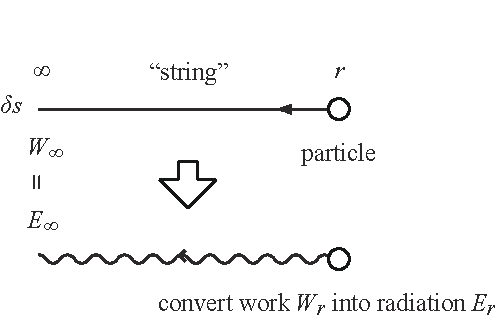
\includegraphics{Ch3_surface_gravity.pdf} }
\vskip2mm
\caption{
In order to obtain the surface gravity, the asymptotic observer pulls the particle by a massless ``string." The work done to the particle is then converted into radiation. The radiation is subsequently collected at infinity. 
%�\�ʏd�͂����߂�D����������u�Ђ��v�ŕ��̂���������C������ꂽ�d������˂ɂ����C�������ʼn������D
}
\label{fig:surface_gravity}
\end{center}
\end{figure}
%%============

The surface gravity is the force (per unit mass) $a_\infty(r_0)$, which is necessary to hold the particle at the horizon by an \textit{asymptotic observer}. In order to obtain the force, suppose that the asymptotic observer pulls the particle at $r$ by a massless ``string" (\fig{surface_gravity}). If the observer pulls the string by the proper distance $\delta s$, the work done is given by
%�\�ʏd�͂Ƃ́C���������̊ϑ��҂��z���C�Y���ł̕��̂�ێ����邽�߂ɕK�v�ȁi�P�ʎ��ʂ�����́j�� $a_\infty(r_0)$ �ł���D��������߂邽�߂ɁC�ʒu$r$�̕��̂����ʃ[���́u�Ђ��v�Ŗ��������̊ϑ��҂����������Ă���Ƃ���i\fig{surface_gravity}�j�D���܁C�ŗL���� $\delta s$ ���������������Ƃ���ƁC������ꂽ�d����
\begin{alignat}{2}
%
W_\infty &= a_\infty \delta s & \quad & (\text{asymptotic infinity})~, \\
W_r &= a \delta s & \quad & (\text{location }r)~.
%\label{eq:}
%
\end{alignat}
Now, convert the work $W_r$ into radiation with energy $E_r=W_r$ at $r$, and then collect the radiation at infinity. The energy received at infinity, $E_\infty$, gets the gravitational redshift (\sect{red_shift}). \index{gravitational redshift} The redshift formula is \eq{red_shift}:
%������ꂽ�d��$W$���C�ʒu$r$�ŕ��� $E=W$ �ɂ����Ė��������ʼn������D���������Ŏ󂯂Ƃ�G�l���M�[$E_\infty$ �́C\sect{red_shift}�̏d�͐ԕ��Έ�\index{���䂤��悭�����ق��ւ�@�d�͐ԕ��Έ�}�ɂ��
\be
%
\frac{E_B}{E_A} =\sqrt{\frac{g_{00}(A)}{g_{00}(B)}}~.
%\label{eq:red_shift}
%
\ee
So, $E_\infty$ is given by
\be
%
E_\infty = \sqrt{ \frac{f(r)}{f(\infty)} } E_r = f(r)^{1/2} a \delta s~,
\label{eq:red_shift_surface}
%
\ee
where we used $f(\infty)=1$. The energy conservation requires $W_\infty=E_\infty$, so $a_\infty=f^{1/2}a =f'/2$ or
%������$f(\infty)=1$���g�����D�������C�G�l���M�[�ۑ������ $W_\infty=E_\infty$�łȂ���΂����Ȃ��D���������āC$a_\infty=f^{1/2}a =f'/2$�C�‚܂�
\be
%
\kappa := a_\infty (r_0) = \frac{f'(r_0)}{2}~,
\label{eq:surface_gravity}
%
\ee
which coincides with the naive result \eqref{eq:surface_gravity_naive}.
%�ƂȂ�C�i�C�[�u�Ȍ��� \eqref{eq:surface_gravity_naive} �ƈ�v����D


%%------------------
\subsection{First law}
%��1�@��}
%%------------------

If the black hole mass increases by $dM$, the horizon area increases by $dA$ as well. So, one has a relation
%���܁C�u���b�N�z�[���̎��ʂ� $dM$ �����������Ƃ���ƁC����ɂ���ăz���C�Y���̖ʐς� $dA$ ����������D���������āC
\be
%
dM \propto dA~.
%
\ee
To have a precise equation, compare the dimensions of both sides of the equation. First, the left-hand side must be $GdM$ because the Newton's constant and mass appear only in the combination $GM$ in general relativity. The Einstein equation tells how the mass energy curves the spacetime, and $G$ is the dictionary to translate from the mass to the spacetime curvature. 

Then, one can easily see that the right-hand side must have a coefficient which has the dimensions of acceleration. It is natural to use the surface gravity for this acceleration. In fact, the first law $dE=TdS$ tells us that temperature appears as the coefficient of the entropy, and we saw earlier that the surface gravity plays the role of temperature. Thus, we reach
%�Ƃ����֌W�����藧�‚ł��낤�D����𓙍��Ō��Ԃ��߂ɂ́C���������킹��K�v������D�܂����ӂ� $GdM$ �ƂȂ�D�ƌ����̂��C��ʑ��Θ_�ł͎��ʂ̓j���[�g���萔�ƈꏏ�ɂ�����邩��ł���D�A�C���V���^�C���������́C���ʃG�l���M�[��������ǂ��Ȃ��邩�������邪�C$G$ �͎��ʂ�����̋Ȃ���ɖ|�󂷂�ʂł���D���̂悤�� $G$ �� $M$ �͈ꏏ�ɂ������D��������ƁC�E�� $dA$ �̌W���Ƃ��āC�����x�̎������������ʂ��K�v�Ȃ��Ƃ������ɂ킩��D���̉����x�Ƃ��āC�����قǏo�Ă����\�ʏd�͂��g���͎̂��R�ł��낤�D���ہC$A$ �̓G���g���s�[�̂悤�ȗʂł��邪�C�M�͊w�̑�1�@���ł� $dE=TdS$ �Ȃ̂ŃG���g���s�[�ɉ��x��������D�����قǁC�\�ʏd�͉͂��x�̖������ɂȂ��Ă��邱�Ƃ��݂��̂ŁC���̈Ӗ��ł��\�ʏd�͂��o�Ă���͎̂��R�ł���D���̂���
\be
%
GdM \simeq \kappa dA~.
%
\ee
By differentiating \eq{horizon_area} with respect to $M$, one can see that
%�ƂȂ邾�낤�D���ۂɁC\eq{horizon_area} ���������΁C���萔�܂œ����
\be
%
GdM = \frac{\kappa}{8\pi} dA
\label{eq:1st_law}
%
\ee
including the numerical constant. This is the \textit{first law of black holes.} \index{first law of thermodynamics (black hole)}
%�Ƃ����������藧�‚��Ƃ��ȒP�ɂ킩��D���ꂪ�u���b�N�z�[����{\bf ��1�@��}\index{�˂‚肫��������1�ق�����@�M�͊w��1�@���i�u���b�N�z�[���j}�ł���D

We discuss the third law of black holes in \sect{RN}.
%�Ȃ��C�u���b�N�z�[���̑�3�@���ɂ‚��ẮC\sect{RN}�ŋc�_����D


%%%%%%%%%%%%%%%%%%%%%%
\section{From analogy to real thermodynamics}
%�A�i���W�[����M�͊w��}
%%%%%%%%%%%%%%%%%%%%%%

%%------------------
\subsection{Hawking radiation
%�z�[�L���O����
}\label{sec:BH_entropy}
%%------------------

We have seen that black hole laws are similar to thermodynamic laws. However, so far this is just an analogy. The same expressions do not mean that they represent the same physics. Indeed, there are several problems to identify black hole laws as thermodynamic laws: 
%���̂悤�Ƀu���b�N�z�[���̖@���́C�M�͊w�̖@���Ƃ悭���Ă���D�������C���̂܂܂ł͂���͒P�Ȃ�A�i���W�[�ɂ����Ȃ��D���̌`���������Ƃ������Ƃ́C�������̂�����킵�Ă��邱�Ƃɂ͂Ȃ�Ȃ��D�����C���̂܂܂ł̓u���b�N�z�[���̖@����M�͊w�̖@���Ƃ��Ă݂�ɂ͂����‚����_������F
\begin{enumerate}
\item 
Nothing comes out from a black hole. If the black hole really has the notion of temperature, a black hole should have a thermal radiation. 
%�u���b�N�z�[������͂Ȃɂ��o�Ă��Ȃ��͂��ł���D�u���b�N�z�[�����{���̈Ӗ��ʼn��x�����‚̂Ȃ�C�M���˂�����͂��ł���D
\item 
The horizon area and the entropy behave similarly, but they have different dimensions. In the unit $\kB=1$, thermodynamic entropy is dimensionless whereas the area has dimensions. One can make it dimensionless by dividing the area by length squared, but so far we have not encountered an appropriate one.
%�G���g���s�[�ƃz���C�Y���̖ʐς͎����ӂ�܂������邪�C�������Ⴄ�D$\kB=1$ �̒P�ʌn�ł́C�G���g���s�[�͖������ʂ����C�ʐς͎����������Ă���D�Ȃɂ������̓��ł��Ζ������ʂɂȂ邪�C����܂ł̂Ƃ���K���ȗʂ͌�������Ȃ��D
\end{enumerate}

The black hole is not an isolated object in our universe. For example, matter can make a black hole, and the matter obeys quantum mechanics microscopically. So, consider the quantum effect of matter. If one considers this effect, the black hole indeed emits the black body radiation known as the Hawking radiation, and its temperature is given by
%�u���b�N�z�[���͂��̉F���ɒP�Ƃő��݂���킯�ł͂Ȃ��D���Ƃ��΃u���b�N�z�[�������o�����̂�����͂��ł���C���̂悤�ȕ��̂̓~�N���ȃX�P�[���ł͗ʎq�͊w�ɂ��������Ă���D�����̗ʎq���ʂ��l����ƁC���ۂɃu���b�N�z�[���͍��̕��˂��N�����i�z�[�L���O���ˁj�C���̉��x��
\begin{align}
%
\kB T &= \frac{\hbar \kappa}{2\pi c} 
\label{eq:temp_vs_surface} \\
&= \frac{\hbar c^3}{8\pi GM}~, \quad \text{(Schwarzschild black hole).}
%
\end{align}
This is a quantum effect because the temperature is proportional to $\hbar$. We explain later how to derive this temperature, the \keyword{Hawking temperature}. Anyway, once the temperature is determined, we can get the precise relation between the black hole entropy $\Sbh$ and the horizon area $A$. The first law of black hole \eqref{eq:1st_law} can be rewritten as
%Anyway, once the temperature is determined, the first law~\eqref{eq:1st_law} 
%�ŗ^������D�ʎq���ʂ��Ƃ����_�́C���x��$\hbar$�ɔ�Ⴗ�邱�Ƃɔ��f����Ă���D���̉��x�C{\bf �z�[�L���O���x}\index{�ف[���񂭂����@�z�[�L���O���x}���ǂ����߂邩�ɂ‚��ẮC���ƂŐ�������D������ɂ���C���̂悤�ɉ��x�����܂�΁C��1�@��~\eqref{eq:1st_law}
\begin{align}
%
d(Mc^2) &= \frac{\kappa c^2}{8\pi G}dA \\
&= \frac{\hbar\kappa}{2\pi \kB c} \frac{\kB c^3}{4G\hbar}dA
= T \frac{\kB c^3}{4G\hbar}dA~.
%
\end{align}
So, comparing with the first law of thermodynamics $dE=TdS$, one obtains
%fixes the numerical coefficient of $\Sbh$ as 
%���g�����Ƃ�$S_\text{BH}$�̔��W�������܂�F
\be
%
\boxeq{
\Sbh = \frac{A}{4G\hbar} \kB c^3 = \frac{1}{4}\frac{A}{\lpl^2} \kB~.
}
\label{eq:BH_entropy}
%
\ee
Here, $\lpl = \sqrt{G\hbar/c^3} \approx 10^{-35}$m is called the \keyword{Planck length}. The Planck length is the length scale where quantum gravity effects become important. Note that one cannot make a quantity whose dimension is the length from the fundamental constants of classical mechanics alone, $G$ and $c$. The black hole entropy now becomes dimensionless because we divide the area by the Planck length squared. Equation~\eqref{eq:BH_entropy} is called the \textit{area law}. \index{area law (black hole entropy)} 
%������ $\lpl = \sqrt{G\hbar/c^3} \approx 10^{-35} \mbox{���[�g��}$��{\bf �v�����N����}\index{�ӂ�񂭂Ȃ���@�v�����N����}�ƌĂ΂��D�v�����N�����́C�ʎq�d�͗��_�̊�b�I�Ȓ����X�P�[���C�‚܂�ʎq�d�͌��ʂ������͂��߂钷�����ƍl�����Ă���D�ÓT�_�̊�b�萔 $G, c$ �����ł́C�����̎��������—ʂ͍��Ȃ��D\eq{BH_entropy}��{\bf �ʐϑ�}\index{�߂񂹂������ӂ�‚��ف[��@�ʐϑ��i�u���b�N�z�[���E�G���g���s�[�j}�ƌ����D

A few remarks are in order. First of all, our discussion here does not ``derive" $\Sbh$ as the real entropy. Microscopically, the entropy is the measure of the degrees of freedom of a system, but we have not counted microscopic states. We are still assuming that classical black hole laws are really thermodynamic laws.
%�u���b�N�z�[���E�G���g���s�[�ɂ‚��Ă����‚����ӂ��Ă������D�܂����ɁC�����ł̋c�_�� $S_\text{BH}$ �����ۂɃG���g���s�[�Ƃ��āu���o�v�����킯�ł͂Ȃ��D�����I�ɂ́C�G���g���s�[�͌n�̎��R�x�𐔂���ړx�ł��邪�C�����ł͔����I��Ԃ𐔂��グ���킯�ł͂Ȃ��D�ˑR�Ƃ��āC�P�ɌÓT�_�I�ȃu���b�N�z�[���̖@�������ۂɔM�͊w�̖@�����Ɖ��肵�Ă���ɂ����Ȃ��D

% added
Second, 
\begin{itemize}
\item The black hole entropy is proportional to the ``area." 
\item On the other hand, the statistical entropy is proportional to the ``volume" of a system. 
\end{itemize}
This difference is extremely important for AdS/CFT and gives a clue on the nature of microscopic states of black holes. Because these entropies behave differently, a four-dimensional black hole cannot correspond to a four-dimensional statistical system. But the five-dimensional ``area" is the four-dimensional ``volume." Then, a five-dimensional black hole can correspond to a four-dimensional statistical system. Namely, %\textit{the black hole entropy suggests that a black hole can be described by the usual statistical system whose spatial dimension is one dimension lower than the black hole.} 
\begin{center}
\fbox{
\begin{tabular}{l}
First clue of AdS/CFT: \\
The black hole entropy suggests that a black hole can be described by \\ 
the usual statistical system whose spatial dimension is one dimension \\ 
lower than the gravitational theory.
\end{tabular}
}
\end{center}
AdS/CFT claims that this statistical system is a gauge theory. Such an idea is called the \keyword{holographic principle} in general \cite{'tHooft:1993gx,Susskind:1994vu}. The holographic principle is the first clue for AdS/CFT, and we will see another clue, the large-$N_c$ gauge theory, in \sect{large_N}. 
%�܂��C�u���b�N�z�[���E�G���g���s�[�̑傫�ȓ����́C���ꂪ�z���C�Y���́u�ʐρv�ɔ�Ⴗ��_�ł���D����ɑ΂��ē��v�͊w�I�ȃG���g���s�[�́C�n�́u�̐ρv�ɔ�Ⴕ�Ȃ���΂����Ȃ��D���̈Ⴂ��AdS/CFT�ɂƂ��ďd�v�ł���D�܂��C����͔����I��Ԃ̐����ɂ‚��Ă̎肪������^����D���Ȃ킿�C�u���b�N�z�[���́C�ʏ�̓��v�͊w�n�Ƃ��Ă�1�����Ⴂ�����̗��_�ŏ�����”\������������DAdS/CFT�ł́C���̓��v�͊w�n���Q�[�W���_�ł���Ǝ咣����D���̂悤�ȍl������ʂ�{\bf �z���O���t�B�b�N����}\index{�ق낭��ӂ��‚������@�z���O���t�B�b�N����}�ƌ����DAdS/CFT�̓z���O���t�B�b�N�����̈��ł���D

Now, our discussion so far uses the Schwarzschild black hole as an example, but the formula \eqref{eq:BH_entropy} itself is generic. The black hole entropy is \textit{always} given by \eq{BH_entropy} as long as %curvature tensors appear only in the form of the Einstein-Hilbert action
the gravitational action is written by the Einstein-Hilbert action%
\footnote{For a generic gravitational action, the \bh entropy is given by the Wald formula \index{Wald formula} \cite{Wald:1994yp}.}:
%���āC���̋c�_�ł͗�Ƃ��ăV�������c�V���h�E�u���b�N�z�[�����g�������C\eq{BH_entropy}�͓���̃u���b�N�z�[���ɂ͂��Ȃ��D�d�͍�p���A�C���V���^�C��-�q���x���g��p�C�‚܂�
\be
%
\frac{1}{16\pi G_d}\int d^dx \sqrt{-g} R~.
%
\ee
Namely, \eq{BH_entropy} is true not only for black holes in general relativity but also for black holes in string theory and in the other gravitational theories.
%�ŗ^���������C�u���b�N�z�[���E�G���g���s�[�͏��\eq{BH_entropy}�ɂȂ�Ƃ������Ƃ��m���Ă��� \cite{Wald:1994yp}�D�‚܂�C\eq{BH_entropy}�͈�ʑ��Θ_�̃u���b�N�z�[���݂̂Ȃ炸�C�������_�₻�̂ق��̏d�͗��_�ł���������D

%%------------------
\subsection{Hawking temperature and Euclidean formalism
%�z�[�L���O���x�ƃ��[�N���b�h�莮��
}\label{sec:Euclidean}
%%------------------

There are several ways to compute the Hawking temperature. Hawking originally computed it by quantizing matter fields in the black hole background. But the simple way is to require that the Euclidean spacetime be smooth. To do so, one needs a periodic identification in imaginary time, and the temperature is the inverse of this period $\beta$.
%�z�[�L���O���x�����߂�ɂ͂����‚����@������D�z�[�L���O���g�������@�́C�u���b�N�z�[������ŕ������ʎq������Ƃ������̂ł���D�������ȕւȕ��@�́C�v�ʂ����[�N���b�h�����āC���󂪂Ȃ߂炩�Ȃ��Ƃ�v�����邱�Ƃł���D����Ƌ����ԕ����Ɏ������E�������K�v�ɂȂ邪�C�u���b�N�z�[���̉��x�͂��̎��� $\beta$ �̋t�ŗ^������D

By the analytic continuation to Euclidean signature $\tE = it$, the metric \eqref{eq:metric_ansatz} becomes 
%�v�� \eqref{eq:metric_ansatz} �� $\tE = it$ �ƃ��[�N���b�h�������
\be
%
ds_\text{E}^2 = + f(r) d\tE^2 + \frac{dr^2}{f(r)} +\cdots~.
%\label{eq:}
%
\ee
Let us focus on the region near the ``horizon" $r \simeq r_0$. Near the horizon, $f(r_0)=0$, so one can approximate%
\footnote{Here, we assume $f'(r_0)\neq 0$. This assumption fails for extreme black holes \index{extreme black hole} where two horizons are degenerate (\sect{RN}). }
$f \simeq f'(r_0) (r-r_0)$. Then,
%���܁u�z���C�Y���v�ߖT $r \simeq r_0$�����ɒ��ڂ���D�z���C�Y���ł� $f(r_0)=0$�Ȃ̂�$f \simeq f'(r_0) (r-r_0)$�ƂȂ�\footnote{������$f'(r_0)\neq 0$ �����肵�Ă���D���̉���́C2�‚̃z���C�Y�����k�ނ��Ă���Ɍ��u���b�N�z�[��\index{���悭����ӂ�‚��ف[��@�Ɍ��u���b�N�z�[��}�i\sect{RN}�j�ł͖�������Ȃ��D}�D���������āC
\begin{align}
%
ds_\text{E}^2 
&\simeq \frac{dr^2}{f'(r_0) (r-r_0)} + f'(r_0) (r-r_0) d\tE^2 \\
&= d\rho^2 + \rho^2 d\left( \frac{f'(r_0)}{2} \tE \right)^2~,
\label{eq:polar}
%
\end{align}
where we introduced a new coordinate $\rho := 2\sqrt{ (r - r_0)/f'(r_0) }$. In this coordinate, the metric takes the same form as a plane in polar coordinates if $f'(r_0)\tE/2$ has the period $2\pi$. Otherwise, the metric has a conical singularity at $\rho=0$. The periodicity of $\tE$ is given by $\beta=4\pi/f'(r_0)$ or
%�����ŁC$\rho := 2\sqrt{ (r - r_0)/f'(r_0) }$�Ƃ����V�������W�𓱓������D���̐V�������W�n�ł́C�v�ʂ͋ɍ��W�n $\rho^2d\theta^2+d\rho^2$�Ɠ����`���Ƃ��Ă���C���������� $f'(r_0)\tE/2$ �̎����� $2\pi$�ł���΁C����Ȃ镽�R�ȋ�Ԃł���D�Ⴄ�������Ƃ��$\rho=0$�𒸓_�Ƃ����u�~���`�v�ɂȂ��Ă��܂��D���������āC$\tE$�̎����� $\beta=4\pi/f'(r_0)$���Ȃ킿
\be
%
\boxeq{
T=\frac{f'(r_0)}{4\pi}~.
}
\label{eq:Hawking_temp}
%
\ee
If one compares this result with \eq{surface_gravity}, one gets $T=\kappa/(2\pi)$ which is \eq{temp_vs_surface}. For the Schwarzschild black hole, $f(r)=1-r_0/r$, so 
%$T=1/(4\pi r_0)=1/(8\pi GM)$. 
\be
%
T = \frac{1}{4\pi r_0} = \frac{1}{8\pi GM}~.
%\label{eq:}
%
\ee
Note that the Euclidean metric does not cover inside the horizon $r<r_0$ since the horizon is the origin of polar coordinates.
%�Ɨv������D\eq{surface_gravity} �Ɣ�ׂ�ƁC$T=\kappa/(2\pi)$ �ƂȂ�\eq{temp_vs_surface}���������D�V�������c�V���h�E�u���b�N�z�[���̏ꍇ�C$f(r)=1-r_0/r$ �Ȃ̂� $T=1/(4\pi r_0)=1/(8\pi GM)$�ł���D���[�N���b�h�������v�ʂł́C�z���C�Y���͋ɍ��W�̌��_�Ȃ̂ŁC�z���C�Y���̓���$r<r_0$���܂܂Ȃ����Ƃɒ��ӁD

What is behind the Euclidean formalism is quantum statistical mechanics. In quantum statistical mechanics, the periodicity in the imaginary time is naturally associated with the inverse temperature. We mimic this technique of quantum statistical mechanics and apply to black holes. Then, the ``first-principle" computation of black hole thermodynamic quantities is carried out as follows \cite{Gibbons:1976ue}. (This approach naturally leads to the \keyword{GKP-Witten relation} in AdS/CFT later.) 
%���̃��[�N���b�h���̎�@�̔w�i�ɂ���̂͗ʎq���v�͊w�ł���D�ʎq���v�͊w�ł͋����Ԃ̎��������x�̋t���Ǝ��R�Ɍ��т‚��D�����Ńu���b�N�z�[���̔M�͊w�ʂ��u��ꌴ���v�I�ɋ��߂�ɂ́C�ȉ��̂悤�ɂ����Ȃ�\cite{Gibbons:1976ue}�D�܂��C���̕��@�͂��Ƃ�AdS/CFT��{\bf GKP-�E�B�b�e���֌W��}\index{GKP�����‚Ă񂩂񂯂�����@GKP-�E�B�b�e���֌W��}�ւƎ��R�ɂ‚Ȃ���D

The problem of quantum gravity is not completely solved, but it is natural to expect that quantum gravity is defined by a path integral such as
%���݁C�ʎq�d�͂̒莮���͊��S�ɂ͉������Ă��Ȃ����C
\be
%
Z = \int {\cal D}g\, e^{i\action_\text{L}[g]}~.
%\label{eq:}
%
\ee
Here, $\action_\text{L}$ is the gravitational action, and the above equation shows the path integral over the metric $g$ schematically. We consider the Euclidean formalism with $\tE=it$, $\action_\text{E}=-i\action_\text{L}$:
%�̂悤�ȔĊ֐��ϕ��ŗ^������ƍl����̂����R�ł���D�����ŁC$g$�͌v�ʁC$\action_\text{L}$ �͏d�͗��_�̍�p�ŁC��̎��͌v�ʂɂ‚��Ă̔Ċ֐��ϕ���͎��I�ɂ���킵�Ă���D�����ł� $\tE=it$, $\action_\text{E}=-i\action_\text{L}$ �Ƃ������[�N���b�h�莮���ōl����F
\be
%
Z = \int {\cal D}g\, e^{-\action_\text{E}[g]}~.
\label{eq:Euclidean}
%
\ee
As we saw above, the Euclidean black hole is periodic in time. Then, it is natural to associate the statistical mechanical partition function \index{partition function} to the black hole and is natural to regard $Z$ as such a partition function. However, it is not clear how to carry out the path integral because it diverges. Also, string theory does not evaluate \eq{Euclidean} itself. In any case, whether one uses string theory or uses the above approach, semiclassical results themselves should agree. Semiclassically, the most dominant contribution to the path integral comes from an extremum of the action, or the classical solution (saddle-point approximation). Under the approximation, 
%���[�N���b�h�������u���b�N�z�[���ł͎��ԕ����̎��������R�ɏo�Ă���̂ŁC�u���b�N�z�[���ɓ��v�͊w�I�ȕ��z�֐�\index{�ӂ�͂����񂷂�@���z�֐�}��Ή������C$Z$�����̂悤�ȕ��z�֐��Ƃ��Ă݂Ȃ��̂����R�ł���D�����Ƃ��C���U�̖��Ȃǂ�����C���̔Ċ֐��ϕ��𐳎��ɂ͂ǂ����s����΂����̂��͕s���ł���D�܂��C�������_��\eq{Euclidean}���̂�]������킯�ł͂Ȃ��D������ɂ���C���ÓT�_�I�ɂ́C�Ċ֐��ϕ��ɂ����Ƃ���^����̂́C��p�̋ɒl�C���Ȃ킿�ÓT���ŋߎ��ł���ł��낤�i�Ɠ_�ߎ��j�D���̋ߎ��̉��ŁC
\be
%
\boxeq{
Z \simeq e^{-\SosE}~.
}
%\label{eq:}
%
\ee
Here, $\SosE$ is the on-shell action which is obtained by substituting the classical solution to the action. The free energy\index{free energy} $F$ is then given by $\SosE=\beta F$. For example, for the Schwarzschild black hole, one can show that 
\be
%
F = \frac{r_0}{4G} = \frac{1}{16\pi G T}~.
\label{eq:free_Sch}
%
\ee
Then, one can get thermodynamic quantities:
\begin{align}
%
\Sbh &= - \del_T F = \frac{1}{16\pi G T^2} = \frac{\pi r_0^2}{G} = \frac{A}{4G}~, \\
E &= F + T \Sbh = \frac{1}{8\pi G T} = \frac{r_0}{2G} = M~.
%\label{eq:}
%
\end{align}
%������ $\SosE$ �́C�v�ʂ̌ÓT���������� on-shell ��p�ł���D���̂悤�Ɍv�Z�������z�֐�����C
%\begin{align}
%
%E &= - \frac{ \del \ln Z }{\del\beta}~, \\
%S_\text{BH} &=  \ln Z + \beta E~.
%\label{eq:}
%
%\end{align}
%�Ȃǂ��g���ĔM�͊w�ʂ��v�Z�ł���D�܂��C���R�G�l���M�[\index{���䂤���˂邫�[@���R�G�l���M�[}$F$�� $\SosE=\beta F$�ŗ^������D

We will not carry out the actual computation for the Schwarzschild black hole here but will carry out for the Schwarzschild-AdS$_5$ black holes in \sect{SAdS_free} and \sect{HP}. AdS/CFT identifies the black hole partition function $Z$ as the gauge theory partition function.
%�V�������c�V���h�E�u���b�N�z�[���ɑ΂��āC�����ł͎��ۂ̌v�Z�͂����Ȃ�Ȃ����C\sect{SAdS_free}�ŃV�������c�V���hAdS$_5$�u���b�N�z�[���ɑ΂��Ă����Ȃ��D���̂悤�ɂ��Čv�Z����$Z$���Q�[�W���_�̕��z�֐��Ɠ��肷��̂��CAdS/CFT�ł���D

%%------------------
\subsection{On the origin of black hole entropy \advanced}
%�u���b�N�z�[���E�G���g���s�[�̋N���ɂ‚���}
%%------------------

What represents the black hole entropy? It is not easy to answer to the question as we will see below, but let us make some general remarks.
%�u���b�N�z�[���E�G���g���s�[�͉�������킵�Ă���̂��낤�H�@�ȉ��݂�悤�ɁC���̖₢�ɓ�����̂͊ȒP�ł͂Ȃ����C��ʓI�ȃR�����g�����Ă������D

When we are speaking of the entropy of the sun, the meaning is clear. Although a thermodynamic system looks same macroscopically, the system can have different microscopic states. There are number of ways one can distribute, \eg, a given energy to a multiple number of particles. The entropy counts the number of possible quantum states when macroscopic variables such as energy are specified. In general, this number becomes larger when the number of particles becomes larger. So, the entropy is generically proportional to the number of particles.
%���Ƃ��΁C���z�̃G���g���s�[�ƌ����ꍇ�C�Ӗ��͖��炩�ł���D����M�͊w�n�������I�ɂ͓�����Ԃɂ݂��Ă��C�����I�ɂ͂��܂��܂ȏ�Ԃ��Ƃ肤��D�G�l���M�[�𕡐��̗��q�ŕ��z����d���́C���낢�날�邩��ł���D�G���g���s�[�́C�^����ꂽ�����I�ϐ��i���Ƃ��΃G�l���M�[�j�ɑ΂��Ĕ����I��Ԃ��ǂꂾ�����邩�𐔂���D���̂悤�ȏꍇ�����̐��́C��ʂɗ��q���������Ȃ�قǑ����Ȃ�D���������āC��ʂɃG���g���s�[�͗��q���ɔ�Ⴗ��D

This suggests that the black hole entropy counts the microscopic states a black hole can have. This number can be estimated as follows \cite{Zurek:1985gd}.
%\footnote{The following argument simplifies the one in Ref.~\cite{Zurek:1985gd}.}.
Let us imagine to make a black hole by collecting particles in a small region. The entropy is proportional to the number of particles. To have a larger entropy, we let the total number of particles as many as possible, or we make the black hole from light particles. However, the Compton wavelength of a particle with mass $m$ is about $\lambda \simeq \hbar/m$. We cannot collect particles in a smaller region than the Compton wavelength. But to make a black hole, we must collect them within the Schwarzschild radius. Thus, if the Compton wavelength is larger than the Schwarzschild radius, a black hole is not formed. Consequently, we cannot choose the particle mass freely, and the lightest particle we can use has mass which satisfies $\hbar/m \simeq 2GM$. Then, the total number of particles is given by
%��������ƁC�u���b�N�z�[���E�G���g���s�[�̏ꍇ�C�u���b�N�z�[���̔����I��Ԃ𐔂��Ă���Ɛ��������D�u���b�N�z�[���̔����I��Ԃ́C���̂悤�ɂ��đ傴���ςɌ��ς��邱�Ƃ��ł���%\footnote{�ȉ��̋c�_�́C����~\cite{Zurek:1985gd}��P�����������̂ł���D}�D���܁C���q��1�����ɂ�������W�߂āC�u���b�N�z�[������邱�Ƃɂ��悤�D�G���g���s�[�͗��q���ɔ�Ⴕ���D�G���g���s�[���Ȃ�ׂ��傫������ɂ̓u���b�N�z�[������闱�q���𑽂��C�‚܂�y�����q������΂悢�D���q�̎��ʂ����R�ɑI�ׂ�̂ł���΁C������ł��y�����q���g�����ƂŃG���g���s�[�͂�����ł��傫���Ȃ肻���ł���D�������C���� $m$ �̗��q�̃R���v�g���g���́C$\lambda \simeq \hbar/m$ ���x�ł���D���܁C��X�͗��q���W�߂ău���b�N�z�[������낤�Ƃ��Ă��邪�C���q���R���v�g���g�����x��苷���̈�ɏW�߂邱�Ƃ͂ł��Ȃ��D�Ƃ���ƁC�ǂ�Ȍy�����q���g���Ă��悢�킯�ł͂Ȃ��D�R���v�g���g�����V�������c�V���h���a�����傫�ȗ��q�ł́C���������u���b�N�z�[���ɂ͂Ȃ�Ȃ�����ł���D���������āC�y�����q�Ƃ����Ă��C�Œ�ł� $\hbar/m \simeq 2GM$ �𖞑�����悤�Ȏ��ʂ͕K�v�ɂȂ�D�Ƃ���ƁC���̏ꍇ�̗��q���́C
\be
%
N_{max} \simeq \frac{M}{m} \simeq \frac{M}{\frac{\hbar}{2GM}}  \simeq \frac{(GM)^2}{G\hbar}  \simeq \frac{A}{G\hbar}~,
%
\ee
which is the right order-of-magnitude for the black hole entropy.
%�ƂȂ�C���傤�ǃu���b�N�z�[���E�G���g���s�[���x�̐��ɂȂ�D

This is fine for a rough estimate, but how can one derive the black hole entropy statistical mechanically? The Planck length $\lpl$ appears in the denominator of the area law \eqref{eq:BH_entropy}. This means that the microscopic derivation of the black hole entropy is likely to require quantum gravity. But the formulation of quantum gravity is a difficult problem, so the problem of the black hole entropy is not completely resolved. String theory is the prime candidate of the unified theory including quantum gravity, and string theory can derive the \bh entropy microscopically for some black holes (see, \eg, Refs.~\cite{Horowitz:1996qd,Dabholkar:2012zz} for reviews).
%����͑傴���ςȌ��ς���Ƃ��Ă͂悢���C�ǂ�����΂����ƃu���b�N�z�[���E�G���g���s�[�𓝌v�͊w�I�ɓ��o�ł��邾�낤�H�@�u���b�N�z�[���E�G���g���s�[��\eq{BH_entropy}�̕���ɂ́C�v�����N����$\lpl$���������D���̂��߁C�u���b�N�z�[���E�G���g���s�[���������ɂ́C�{���I�ɗʎq�d�͗��_���K�v���ƍl������D�������C�ʎq�d�͗��_�̒莮���͍���Ȗ��ŁC���܂��Ɋ��S�Ȍ����͂‚��Ă��Ȃ��D���̂��߃u���b�N�z�[���E�G���g���s�[�̖����C���܂��Ɋ��S�ɂ͌������Ă��Ȃ��D�������C�������_�͗ʎq�d�͂��܂߂����ꗝ�_�̍ŗL�͌��ł���C�u���b�N�z�[���E�G���g���s�[�̖��ɂ‚��Ă�������x���������߂Ă���\cite{natsuume99}�D

In \sect{Euclidean}, we briefly discussed the semiclassical computation of the black hole entropy. It is natural that such a computation gives the black hole entropy and is not just a coincidence. There should be something behind which justifies the computation. But one can say that it is not satisfactory as the microscopic derivation of the black hole entropy, namely as the statistical derivation of the black hole entropy: 
\begin{itemize}
\item First, \eq{Euclidean} itself is not well-defined and cannot be estimated beyond the semiclassical approximation. 
\item Also, the computation does not tell us what degrees of freedom the black hole entropy corresponds to. 
\end{itemize}
%\sect{Euclidean}�ł́C�u���b�N�z�[���E�G���g���s�[�̔��ÓT�_�I�v�Z���Љ���D���̂悤�Ȍv�Z����C�u���b�N�z�[���E�G���g���s�[�𓱏o�ł���͎̂��R�ł���C�܂��P�Ȃ���R�Ƃ͍l���ɂ����D�Ȃɂ����̌v�Z�𐳓����ł�����̂��w��ɂ���Ǝv����D�������Ȃ���C���ꂪ�u���b�N�z�[���E�G���g���s�[�̔����I���o���C���Ȃ킿���v�͊w�I�ȈӖ��ł̓��o���Ɩ����΁C�s�����ƌ����č����‚����Ȃ����낤�D���������C\eq{Euclidean}���̂��̂�well-defined�ł͂Ȃ��C���ۂɔ��ÓT�_�I�ߎ��𒴂��ĕ]�����邱�Ƃ͂ł��Ȃ��D�܂��C�u���b�N�z�[���E�G���g���s�[�����̎��R�x�ɑ�������̂������炩�ł͂Ȃ��D

But AdS/CFT gives an interesting interpretation to the semiclassical result. AdS/CFT identifies the partition function computed in this way as the partition function of a gauge theory. AdS/CFT claims the equivalence between two theories, a gauge theory and a gravitational theory, and there are two points of view one can take: 
\begin{itemize}
\item Namely, one can use the gravitational theory to know about the gauge theory. 
\item Or, one can use the gauge theory to know about the gravitational theory. 
\end{itemize}
Because AdS/CFT claims the equivalence, it is hard to say which point of view is more fundamental, namely which theory is more fundamental, but let us take the latter point of view for now. If so, one can regard the origin of the black hole entropy as the entropy of the corresponding gauge theory, namely the number of microscopic states of the gauge theory. Then, the black hole entropy is nothing but the usual statistical entropy. 
%�������CAdS/CFT�͂��̔��ÓT�_�I�Ȍv�Z�ɑ΂��āC�����[�����߂�^����DAdS/CFT�ł́C���̂悤�Ɍv�Z�������z�֐����Q�[�W���_�̕��z�֐��Ƃ��ē��肷��DAdS/CFT��2�‚̗��_�̓��������咣����̂ŁC�i1�j�Q�[�W���_�ɂ‚��Ēm�邽�߂ɏd�͗��_���g���Ƃ�������ƁC�i2�j�d�͗��_�ɂ‚��Ēm�邽�߂ɃQ�[�W���_���g���Ƃ������ꂪ���肤��D�ǂ��炪����{�I�ȗ��_���Ƃ������́C�Ȃ��Ȃ������肾���C�����ł͌�҂̗�����Ƃ��Ă݂悤�D����ƁCAdS/CFT�̗���ł́C�u���b�N�z�[���E�G���g���s�[�̋N���́C�Ή�����Q�[�W���_�̃G���g���s�[�C�‚܂�Q�[�W���_�̔����I��Ԑ����ƍl���邱�Ƃ��ł���D���Ƃ���΁C�u���b�N�z�[���E�G���g���s�[���ʏ�̓��v�͊w�I�ȃG���g���s�[�ɂق��Ȃ�Ȃ��D

However, black holes in AdS/CFT are the ones in AdS spacetime. It is not clear if one can make such an interpretation for any black holes, in particular for the Schwarzschild black hole. The holographic principle seems to suggest that this is somehow possible. 
%�����Ƃ��CAdS/CFT�������u���b�N�z�[���́CAdS���󒆂̃u���b�N�z�[���ł���D�ǂ̂悤�ȃu���b�N�z�[���ɂ‚��Ă��i�Ƃ��ɃV�������c�V���h�E�u���b�N�z�[���ɂ‚��Ă��j�C���̂悤�ȉ��߂��”\���ǂ����͕s���ł��邪�C�z���O���t�B�b�N�����͂��̂��Ƃ���������D

%%%%%%%%%
\section{Other black holes}
%���̂ق��̃u���b�N�z�[��}%\label{sec:}
%%%%%%%%%


%%------------------
\subsection{Higher-dimensional Schwarzschild black holes}
%�������V�������c�V���h�E�u���b�N�z�[��}
\label{sec:higher}
%%------------------

The four-dimensional Schwarzschild black hole can be generalized to $d$-dimensional spacetime:
%�V�������c�V���h�E�u���b�N�z�[���́C��ʂ̎����Ɋg�����邱�Ƃ��ł���F
%\begin{subequations}
%\label{eq:}
\begin{align}
%
ds_d^2 &= - f(r) dt^2 + \frac{dr^2}{f(r)} 
+ r^2 d\Omega_{d-2}^2~,
\label{eq:Schwarzschild_d_dim} \\
f(r) &= 1-\left(\frac{r_0}{r}\right)^{d-3} = 1- \frac{16 \pi G_d}{(d-2) \Omega_{d-2}} \frac{M}{r^{d-3}}~,
\label{eq:Schwarzschild_d_mass} \\
\Omega_n &= \frac{2\pi^{\frac{n+1}{2}}}{\Gamma(\frac{n+1}{2})}~.
%\label{eq:}
%
\end{align}
%\end{subequations}
Here, $G_d$ is the Newton's constant in $d$-dimensional spacetime, $d\Omega_n^2$ is the line element of the unit $S^n$ (see \sect{higher_AdS} for an explicit construction), and $\Omega_n$ is its area which is written by the Gamma function $\Gamma(n+1/2)$. Some explicit forms of $\Omega_n$ are given by
%$G_d$ ��$d$��������̃j���[�g���萔�C$\Omega_n$ �� $S^n$ �̖ʐςŃK���}�֐� $\Gamma(n+1/2)$ �ŏ�����D�����‚��� $\Omega_n$ �̒l�������Ă����ƁC
\begin{gather}
%
\Omega_0 = 2~, \quad
\Omega_1 = 2 \pi~, \quad
\Omega_2 = 4 \pi~, \quad
\Omega_3 = 2 \pi^2~, \nonumber \\
\Omega_4 = \frac{8}{3} \pi^2~, \quad
\Omega_5 = \pi^3~, \quad
\Omega_6 = \frac{16}{15} \pi^3~, \quad
\Omega_7 = \frac{1}{3} \pi^4~.
\ldots
%
\end{gather}
The behavior $1/r^{d-3}$ in $f(r)$ comes from the fact that the Newtonian potential behaves as $1/r^{d-3}$ in $d$-dimensional spacetime. 
%$f(r)$ �� $1/r^{d-3}$ �́C$d$�����Ńj���[�g���E�|�e���V������ $1/r^{d-3}$ �ƐU��܂����Ƃ𔽉f���Ă���D

Using Eqs.~\eqref{eq:BH_entropy} and \eqref{eq:Hawking_temp}, one gets thermodynamic quantities:
%�M�͊w�ʂ�\eq{BH_entropy}�C\eqref{eq:Hawking_temp}���g���C
\begin{align}
%
T &= \frac{f'(r_0)}{4\pi} 
= \frac{d-3}{4\pi r_0}~,
\label{eq:temp_Sch_d} \\
\Sbh &= \frac{A}{4G_d} 
= \frac{r_0^{d-2} \Omega_{d-2}}{4G_d}~.
\label{eq:entropy_Sch_d}
%M &= \frac{(d-2) \Omega_{d-2}}{16 \pi G_d} r_0^{d-3}~.
%\label{eq:}
%
\end{align}
One can check the first law with these quantities and the mass \eqref{eq:Schwarzschild_d_mass}.


%%------------------
\subsection{Black branes}\label{sec:black_branes}
%%------------------

The black holes in previous subsection are simply the extensions of the four-dimensional black hole, but in higher dimensions, there exist black holes which do not appear in four-dimensions. The Schwarzschild \bh has a spherical horizon, but the horizon can take other topologies in higher dimensions%
\footnote{For four-dimensional asymptotically flat black holes, the topology of black hole horizons must be $S^2$ under appropriate conditions on matter fields. This is known as the \keyword{topology theorem} (see, \eg, Proposition 9.3.2 of Ref.~\cite{HE}) which is part of the no-hair theorem. }.
In particular, the horizon can have an infinite extension. 

A simple example is the five-dimensional ``neutral black string," which is the four-dimensional Schwarzschild \bh times $\mathbb{R}$:
\be
%
ds_5^2 = - \left(1-\frac{r_0}{r} \right) dt^2 + \frac{dr^2}{1-\frac{r_0}{r}} + r^2 d\Omega_2^2 + dz^2~,
\label{eq:black_string}
%
\ee
where $z$ represents the $\mathbb{R}$ coordinate. For the five-dimensional Schwarzschild black hole, the horizon, the $r=r_0$ surface has the line element $r_0^2 d\Omega_3^2$ which represents the $S^3$-horizon. Here, the horizon is still given by $r=r_0$, but the horizon has the line element $r_0^2 d\Omega_2^2 + dz^2$. So, the horizon has the topology $S^2\times\mathbb{R}$ and extends indefinitely in $z$-direction. Such a horizon is called a \keyword{planar horizon}. When we say the word ``black hole" in this book, it is mostly a \bh with a planar horizon. A black hole with planar horizon is often called a \keyword{black brane}.

The black branes arise with various dimensionalities. A black brane with $\mathbb{R}^p$ horizon is called a black $p$-brane. Namely, 
\begin{center}
\begin{tabular}{cc}
%
$ p=0 $		& black hole \\
$ p=1 $		& black string \\
$ p=2 $		& \hspace{5mm} black membrane \\
$ \vdots $	& $ \vdots $
%
\end{tabular}
\end{center}
To obtain thermodynamic quantities of the neutral black string, notice that the black string is just the four-dimensional Schwarzschild \bh if one compactifies the $z$-direction. Then, the black string and the four-dimensional Schwarzschild \bh have the same thermodynamic quantities. Take the periodicity of $z$ as $V_1$. By the compactification,
\be
%
\frac{1}{16\pi G_{5}} \int d^{5}x \sqrt{-g_{5}}R_{5} 
=
\frac{V_1}{16\pi G_{5}} \int d^{4}x \sqrt{-g_{4}}\left(R_{4} +\cdots \right)~, 
%\label{eq:}
%
\ee
where the dots denote matter fields which appear by the compactification. Thus, the four-dimensional Newton's constant $G_4$ is written as $1/G_4=V_1/G_5$ from the five-dimensional point of view. Then, thermodynamic quantities are
\be
%
T = \frac{1}{4\pi r_0}~, \quad
S = \frac{\pi r_0^2}{G_4} = \frac{\pi r_0^2}{G_5}\, V_1~, \quad
M = \frac{r_0}{2G_4} = \frac{r_0}{2G_5}\, V_1~, \quad
P= - \frac{r_0}{4G_5}~,
\label{eq:black_string_thermo}
%
\ee
where we used the first law $dM=TdS-PdV_1$ to derive the pressure $P$. The entropy of the black string is rewritten as 
\be
%
S_\text{string} = 4\pi G_5 \frac{M^2}{V_1}~.
\label{eq:black_string_fund}
%
\ee


%%------------------
\subsubsection*{Gregory-Laflamme instability \advanced}%\label{sec:}
%%------------------

As a side remark, the neutral black string actually has the so-called \keyword{Gregory-Laflamme instability} \cite{Gregory:1993vy} (see, \eg, Refs.~\cite{Horowitz:2012nnc2,Harmark:2007md} for reviews). The black string is not the only neutral solution allowed, but the five-dimensional Schwarzschild \bh is also allowed.
%\be
%
%ds_5^2 = - \left\{1-\left(\frac{\tilr_0}{r}\right)^2 \right\} dt^2 + \frac{dr^2}{1-\left(\frac{\tilr_0}{r}\right)^2} + r^2 d\Omega_3^2~.
%\label{eq:}
%
%\ee
Even though the $z$-direction is compactified, the metric \eqref{eq:Schwarzschild_d_dim} should be good approximately when the horizon radius $\tilr_0$ satisfies $\tilr_0 \ll V_1$. The thermodynamic quantities behave as
\be
%
M \simeq \frac{\tilr_0^2}{G_5}~,  \quad
S_\text{BH$_5$} \simeq \frac{\tilr_0^3}{G_5} \simeq \sqrt{G_5}M^{3/2}~.
%\label{eq:}
%
\ee
On the other hand, the entropy of the black string behaves as \eq{black_string_fund}. Consider the microcanonical ensemble with fixed $M$. Then, $S_\text{BH$_5$}>S_\text{string}$ for a large enough $V_1$, so the \bh is favorable entropically. Then, the black string is unstable and would decay to the black hole, but it is still not clear if the transition really occurs (\fig{GL_instability}). Anyway, it has been shown numerically that the neutral black string is unstable under perturbations%
\footnote{It has been argued that the Gregory-Laflamme instability is related to the Rayleigh-Plateau instability in hydrodynamics \cite{Cardoso:2006ks}. \index{Rayleigh-Plateau instability}}.

%%============
\begin{figure}[tb]
\centering
\scalebox{0.75}{ 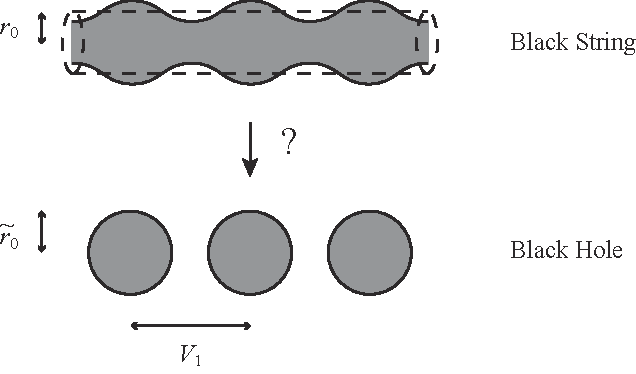
\includegraphics{Ch3_GL_instability.pdf} }
\caption{Gregory-Laflamme instability.}
\label{fig:GL_instability} 
\end{figure}%
%%============

%%------------------
\subsection{Charged black holes
%�דd�u���b�N�z�[��
}\label{sec:RN}
%%------------------

%So far we considered the simplest black holes, Schwarzschild black holes, but 
A black hole can have a charge $Q$. The solution is known as the \keyword{Reissner-Nordstr\"{o}m black hole} (RN black hole hereafter):
%����܂ŁC�����Ƃ��ȒP�ȃu���b�N�z�[���C�V�������c�V���h�E�u���b�N�z�[�����l���Ă������C�u���b�N�z�[���ɓd�� $Q$ ���������邱�Ƃ��”\�ł���D�����{\bf ���C�X�i�[-�m���h�X�g�����[��}�iReissner-Nordstr\"{o}m�j{\bf �E�u���b�N�z�[��}\index{�炢���ȁ[�̂�Ƃ��Ƃ��[�ނӂ�‚��ف[��@���C�X�i�[-�m���h�X�g�����[���E�u���b�N�z�[��}�ƌ����F
%\mathindent=0zw % <-- [1]
%\begin{subequations}
%\label{eq:}
\begin{align}
%
ds^2 &= - \left( 1-\frac{2GM}{r}+\frac{GQ^2}{r^2} \right) dt^2 
+ \frac{dr^2}{1-\frac{2GM}{r}+\frac{GQ^2}{r^2}} + r^2 d\Omega_2^2 
\\
&= - \left( 1-\frac{\ro}{r} \right)\left( 1-\frac{\ri}{r} \right) dt^2 
+ \frac{dr^2}{\left( 1-\frac{\ro}{r} \right)\left( 1-\frac{\ri}{r} \right)} + r^2 d\Omega_2^2~,
\label{eq:RN} \\
F_{r0} &= \frac{Q}{r^2}~,
\label{eq:RN_Maxwell}
%
\end{align}
%\end{subequations}
%\mathindent=2zw % <-- [2] �f�t�H���g
where $2GM = \ro+\ri$ and $GQ^2 = \ro \ri$. We chose the dimensions of $Q$ as dimensionless. (The charge is dimensionless in the units $c=\hbar=1$.) 

The RN black hole is a solution of the Einstein-Maxwell theory%
\footnote{Note the normalization of the Maxwell action. This choice is standard for the RN black hole.}: 
%$2GM = \ro+\ri, Q^2 = \ro \ri$�ł���D
%GQ^2�̏ꍇ�F������ $Q$ �̎����́C�ÓT�͊w�̓d�ׂ̎����Ɉ�v����悤�ɑI�񂾁D$c=1$�̒P�ʌn�ł́C$G = [L M^{-1}]$�Ȃ̂�$Q^2=[LM]$�D
%���C�X�i�[-�m���h�X�g�����[���E�u���b�N�z�[���i�ȉ�RN�u���b�N�z�[���j�́C�A�C���V���^�C��-�}�N�X�E�F�����_
\be
%
\action = \int d^{4}x\, \sqrt{-g} \left( \frac{1}{16\pi G} R - \frac{1}{16\pi} F^2 \right)~.
%\label{eq:}
%
\ee
The equations of motion from the above action is given by
% �̉��ł���D�^����������
\begin{align}
%
R_{\mu\nu} - \frac{1}{2} g_{\mu\nu} R 
&= 2G\left( F_{\mu\rho} F_\nu^{~\rho} - \frac{1}{4} g_{\mu\nu} F^2 \right)~, \\
\nabla_\nu F^{\mu\nu} &= 0~.
%\label{eq:}
%
\end{align}
%�ŗ^������D
Here, we check only the Maxwell equation:
%�����ł́C��̌v�ʂŃ}�N�X�E�F��������
\be
%
\nabla_\nu F^{\mu\nu} = \frac{1}{\sqrt{-g}} \del_\nu(\sqrt{-g}F^{\mu\nu}) = 0~.
%\label{eq:}
%
\ee
When a black hole has an electric charge, $F_{r0}=E_r \neq 0$, and the only nontrivial equation is $\del_r(\sqrt{-g}F^{r0}) = 0$. For the above metric, $F^{r0}=-F_{r0}$ and $\sqrt{-g} = r^2 \sin^2\theta$, so the solution to the Maxwell equation is given by \eq{RN_Maxwell}.
%�������m�F���Ă����D�d�ׂ����ꍇ�� $F_{r0}=E_r \neq 0$ �Ȃ̂ŁC�񎩖��Ȏ���$\del_r(\sqrt{-g}F^{r0}) = 0$�����ł���D��̌v�ʂ� $F^{r0}=-F_{r0}$�C$\sqrt{-g} = r^2 \sin^2\theta$ �ƂȂ邱�Ƃ��g���ƁC
%\be
%
%F_{r0} = \frac{Q}{r^2}~.
%\label{eq:}
%
%\ee
The field strength $F_{\mu\nu}$ is written by the gauge potential $A_\mu$ as $ F_{\mu\nu} = \del_\mu A_\nu - \del_\nu A_\mu$. For our electric field, one may choose the gauge potential $A_0$ as
\be
%
A_0 = - \frac{Q}{r}~.
%\label{eq:}
%
\ee
%Such an electric field can be obtained by choosing the gauge potential as, \eg, $A_0=-Q/r$ (see below for the choice of the gauge potential further).
%One can get such an electric field by choosing the gauge potential as $A_0=-Q/r$.
%�����ł���D$A_0=-Q/r$ �ƃQ�[�W�E�|�e���V������I�ԂƁC���̂悤�ȓd�ꂪ������D

The black hole \eqref{eq:RN} has two horizons $r=r_\pm$, where 
%�v�� \eqref{eq:RN} �́C
\be
%
r_\pm = GM \pm \sqrt{G^2M^2 - GQ^2}~.
\label{eq:outer&inner}
%
\ee
But note that
%�� $g_{00}(r=r_\pm)=0$ �ƂȂ�C2�‚̃z���C�Y�������D�܂��C���ٓ_�� $r=0$ �ł���D�������C
\begin{itemize}
\item 
When $\sqrt{G}M>Q$, two horizons exist.
%$GM>Q$ �̏ꍇ�z���C�Y�������邪�C
\item
When $\sqrt{G}M<Q$, there is no horizon since \eq{outer&inner} becomes complex.
%$GM<Q$ �̏ꍇ�C\eq{outer&inner}���������������Ȃ��̂Ńz���C�Y�����Ȃ��D
\item
The limiting case $\sqrt{G}M=Q$ or $\ro=\ri$ is called the \keyword{extreme black hole}.
%$GM=Q$�C���邢�� $\ro=\ri$ �̏ꍇ��{\bf �Ɍ��u���b�N�z�[��}\index{���悭����ӂ�‚��ف[��@�Ɍ��u���b�N�z�[��}�iextreme black hole�j�ƌ����D
\end{itemize}
Also, the \bh has a spacetime singularity at $r=0$.

%%------------------
\subsubsection*{Thermodynamic quantities}
%\label{sec:}
%%------------------

Again using Eqs.~\eqref{eq:BH_entropy} and \eqref{eq:Hawking_temp}, one gets
%�M�͊w�ʂ�
\begin{align}
%
T 
%= \frac{f'(r_0)}{4\pi} 
&= \frac{\ro - \ri}{4\pi \ro^2}
= \frac{1}{2\pi} \frac{ \sqrt{G^2M^2-GQ^2} }{ 2GM \left( GM+\sqrt{G^2M^2-GQ^2} \right) - GQ^2 }~, \label{eq:temp_RN} 
\\
\Sbh 
%= \frac{A}{4G} 
&= \frac{ 4\pi \ro^2 }{4G}
= \frac{\pi}{G} \left( GM+\sqrt{G^2M^2-GQ^2} \right)^2~.
\label{eq:entropy_RN}
%
\end{align}
The black holes with $\sqrt{G}M>Q$ emit the Hawking radiation and eventually settle into the extreme black hole. The extreme black hole has zero temperature%
\footnote{
%Readers may have the following question. 
Since the Hawking temperature is proportional to the surface gravity, a zero temperature black hole has zero surface gravity. Then, does the black hole have no gravitational force? As we saw previously, the surface gravity is the gravitational force measured by the asymptotic observer. But the asymptotic observer and the observer near the horizon disagree the value of the force because of the gravitational redshift. Although there is a gravitational force for the observer near the horizon, it vanishes for the asymptotic observer. }.
%$GM>Q$ �̃u���b�N�z�[���́C�z�[�L���O���˂ōŏI�I�ɋɌ��u���b�N�z�[���ւƗ����‚��D�Ɍ��u���b�N�z�[���͉��x0�ł���%
%\footnote{���x�[���̃u���b�N�z�[���ƕ����ƁC��قɎv���邩������Ȃ��D�ƌ����̂́C���x�͕\�ʏd�͂ɔ�Ⴗ��̂ŁC���x�[���̃u���b�N�z�[���Ƃ����͕̂\�ʏd�͂��[���Ƃ������Ƃł���D����͏d�͂̂Ȃ��u���b�N�z�[���Ƃ������Ƃł͂Ȃ��D�����ɏ������悤�ɁC�\�ʏd�͉͂����̐l���������d�͂̂��Ƃł���D�����������̐l�ƁC�z���C�Y���ߖT�ɂ���l�̊Ԃł͏d�͐ԕ��Έڂ̈Ⴂ������D���̂��߁C�z���C�Y���ߖT�ɂ���l�ɂ͏d�͂������Ă��Ă��C�����̐l�ɂ͏d�͂������Ă��Ȃ��悤�Ɍ����邾���ł���D}�D

When a thermodynamic system exchanges particle numbers or charges with the environment, the first law becomes
\be
%
dM = T d\Sbh + \mu dQ~,
\label{eq:1st_law_charged}
%
\ee
where $\mu$ is the ``chemical potential." This is just the gauge potential $A_0$ in this case. However, the value of $A_0$ itself is not meaningful due to the gauge invariance:
\be
%
A_0(x) \to A_0(x) + \del_0 \Lambda(x)~.
\label{eq:bulk_gauge}
%
\ee
What is physical is the difference of the gauge potential. 

Imagine to add a charge $\Delta Q$ from the asymptotic infinity to the black hole. This requires energy $\Delta E$ proportional to the difference of $A_0$ between the asymptotic infinity and the horizon (for a same sign charge as the black hole). Then, $\mu$ should be given by
\be
%
\mu = \left. A_0 \right|_{r=\infty} - \left. A_0 \right|_{r=\ro}~,
\label{eq:def_chemical1}
%
\ee
and $\Delta E = \mu\Delta Q$ which takes the form of the first law. Thus,
\be
%
\mu = \frac{Q}{\ro} = \sqrt{ \frac{1}{G}\frac{\ri}{\ro} }~.
%\label{eq:}
%
\ee
Using these thermodynamic quantities, one can show the first law \eqref{eq:1st_law_charged}%
\footnote{On the other hand, for the RN black hole (and for the Schwarzschild black hole), the other thermodynamic relations such as the Euler relation and the Gibbs-Duhem relation do not take standard forms (\sect{BH_fund_rels}).}.
%This is essentially because these black holes do not satisfy fundamental postulates of thermodynamics (\sect{thermodynamics}). In particular, for these black holes, the so-called fundamental relation is \textit{not} a homogeneous first order function of the extensive variables. In contrast, black branes do satisfy fundamental postulates of thermodynamics and obey these thermodynamic relations. }:

%%------------------
\subsubsection*{Third law}
%\label{sec:}
%%------------------

According to the third law of thermodynamics, $S\rightarrow0$ as $T\rightarrow0$ (Nernst-Planck postulate). On the other hand, the entropy of the RN black hole remains finite as $\sqrt{G}M\rightarrow Q$, so the black hole seems to violate the third law.\index{third law of thermodynamics (black hole)} 

This point is still controversial, but a finite entropy at zero temperature means that ground states are degenerate, and there is nothing wrong about degenerate ground states quantum mechanically. However, such a degeneracy is often true only in idealized situations, and the degeneracy is normally lifted by various perturbations. Similarly, the degeneracy of the RN black hole may be lifted by various interactions. 
%This point is still controversial, but two issues are involved. 
%\begin{itemize}
%\item First, if the above argument is true, is the black hole consistent with the third law? 
%\item Second, does the extreme black hole really have a finite entropy? (There are subtleties to take the extreme limit.) 
%\end{itemize}

%First, a finite entropy at zero temperature means that ground states are degenerate and there is nothing wrong about degenerate ground states quantum mechanically. However, such a degeneracy is often true only in idealized situations, and the degeneracy is normally lifted by various perturbations. Similarly, the degeneracy of the RN black hole may be lifted by various interactions. Second, the entropy of the extreme RN black hole has been derived microscopically by using string theory. In such a computation, one counts degenerate ground states, so the computation is consistent with the interpretation that the extreme black hole has a finite entropy. 
%�M�͊w�̑�3�@���ɂ��ƁC$T\rightarrow0$�ƂƂ���$S\rightarrow0$�ł���i�l�����X�g-�v�����N�̉����j�D����C$GM\rightarrow Q$�ł�RN�u���b�N�z�[���̃G���g���s�[�͗L���̂܂܂ł���C��3�@��\index{�˂‚肫��������3�ق�����@�M�͊w��3�@���i�u���b�N�z�[���j}��j���Ă���悤�ɂ݂���D���̓_�ɂ‚��Ă͊��S�ɂ͉������Ă��Ȃ����C�c�_�ɂȂ�̂́C�i1�j��3�@���Ƃ̐������ƁC�i2�j���������Ɍ�RN�u���b�N�z�[�����{���ɗL���̃G���g���s�[�����‚̂��Ƃ����_�ł���i�Ɍ��̂Ƃ���ɔ����ȓ_������j�D�܂��i1�j�̓_�����C$T=0$�ł̗L���̃G���g���s�[�́C����Ԃ��k�ނ��Ă��邱�Ƃ��Ӗ����邪�C����Ԃ̏k�ގ��̂͗ʎq�͊w�I�ɖ��͂Ȃ��D�������C���̂悤�ȏk�ނ͗��z�����ꂽ�ꍇ�ɂ̂ݐ������C�k�ނ͂��܂��܂Ȑۓ��ɂ���Ĉ�ʂɉ����Ă��܂��D���l�ɁCRN�u���b�N�z�[���̏k�ނ����ݍ�p�ɂ���ĉ�����̂�������Ȃ��D���Ɂi2�j�̖��ł��邪�C�������_���g���Ĕ����I��Ԃ̐����グ�Ƃ���RN�u���b�N�z�[���̃G���g���s�[�����o����Ă���\cite{natsuume99}�D�����ł͏k�ނ�������Ԃ𐔂��Ă���̂ŁC�Ɍ��u���b�N�z�[���͗L���̃G���g���s�[�����‚Ƃ������߂Ɩ����͂Ȃ��D

% omitted from Springer edition
%%------------------
%\subsubsection*{The near-horizon limit of the extreme Reissner-Nordstr\"{o}m black hole\index{near-horizon limit}}%\label{sec:}
%%------------------

%The spacetime geometry near the horizon is particularly interesting in the extreme limit. When $\ro=\ri=r_0$, the metric \eqref{eq:RN} becomes
%\be
%
%ds^2 = - \left( 1-\frac{r_0}{r} \right)^2 dt^2 
%+ \frac{ dr^2 }{ \left( 1-\frac{r_0}{r} \right)^2 }
%+r^2 d\Omega_2^2~.
%\label{eq:}
%
%\ee
%Near the horizon $r\rightarrow r_0$, the metric reduces to
%\begin{align}
%
%ds^2 &\rightarrow - \frac{(r-r_0)^2}{r_0^2} dt^2 
%+ r_0^2 \frac{dr^2}{(r-r_0)^2} +r_0^2 d\Omega_2^2
% \\
%&= - \left( \frac{\tilr}{r_0} \right)^{2} dt^2 
%+ r_0^2 \frac{d\tilr^2}{\tilr^2} +r_0^2 d\Omega_2^2~,
%\label{eq:}
%
%\end{align}
%where we made the coordinate transformation $\tilr=r-r_0$. The resulting geometry is AdS$_2 \times S^2$ as we will see later. Thus, the extreme RN black hole is often discussed in AdS/CFT.

%%%%%%%%%
\section{\titlesummary}%\label{sec:}
%%%%%%%%%

\begin{itemize}
\item 
A \bh behaves as a thermodynamic system and has thermodynamic quantities such as energy (mass), entropy, and temperature.
\item 
The \bh entropy is proportional to the horizon area. 
This suggests that a black hole can be described by 
the usual statistical system whose spatial dimension is one dimension 
lower than the gravitational theory (holographic principle).
\item 
To derive \bh thermodynamic quantities, use the Euclidean path integral formulation and evaluate the path integral by the saddle-point approximation.
\item
These are various black objects (black branes) in higher dimensions.
\end{itemize}

%%------------------
\titlenewterms
%%------------------

\begin{multicols}{2}
\noindent
black hole thermodynamics\\
black hole entropy\\
no-hair theorem\\
%zeroth law of thermodynamics (black hole)\\
surface gravity\\
%gravitational redshift\\
%first law of thermodynamics (black hole)\\
Hawking temperature\\
Planck length\\
area law\\
holographic principle\\
%Wald formula\\
%extreme black hole\\
Euclidean formalism\\
%GKP-Witten relation\\
%partition function\\
%free energy\\
planar horizon\\
black brane\\
%Gregory-Laflamme instability\\
%topology theorem\\
Reissner-Nordstr\"{o}m black hole\\
%Rayleigh-Plateau instability\\
extreme black hole
%third law of thermodynamics (black hole)\\
%Smarr's formula\\
%fundamental relation\\
\end{multicols}


%%%%%%%%%
\section{Appendix: Black holes and thermodynamic relations \advanced}\label{sec:BH_fund_rels}
%%%%%%%%%

We saw that black holes satisfy the first law. The first law should be always satisfied because the law simply represents the energy conservation. On the other hand, the other thermodynamic relations such as the Euler relation and the Gibbs-Duhem relation do not take standard forms for black holes with \textit{compact horizon}. The story is different for black branes though: these relations take standard forms like standard thermodynamic systems. 

For example, thermodynamic quantities of the Schwarzschild \bh are given by
\be
%
T = \frac{1}{4\pi r_0}~, \quad
S = \frac{\pi r_0^2}{G_4}~, \quad
E = \frac{r_0}{2G_4}~.
\label{eq:BH_thermo}
%
\ee
So, the Euler relation does not take the form $E=TS$, but 
\be
%
E=2TS~,
%\label{eq:}
%
\ee
which is known as the Smarr's formula.\index{Smarr's formula}

For black holes with compact horizon, thermodynamic relations do not take standard forms because these black holes do not satisfy fundamental postulates of thermodynamics (\sect{thermodynamics}). In particular, thermodynamics requires that the entropy is additive over the subsystems. This requirement is unlikely to hold in the presence of a long-range force such as gravity. Another related problem is that the volume $V$ and its conjugate quantity, pressure $P$, do not appear in those black holes (at least as independent variables.)

The postulate in particular implies that the so-called \keyword{fundamental relation} of a standard thermodynamic system 
\be
%
S = S(E, V)
%\label{eq:fund_entropy}
%
\ee
is a homogeneous \textit{first order} function of extensive variables:
\be
%
S( \lambda E, \lambda V) = \lambda S(E, V)~.
%
\ee
Then, the Euler relation and the Gibbs-Duhem relation follow from the fundamental relation. However, if one rewrites \eq{BH_thermo} in the form of the fundamental relation, one gets
\be
%
S_\text{BH$_4$} = 4\pi G_4 E^2~,
\label{eq:BH_fund}
%
\ee
which is a homogeneous \textit{second order} function in $E$. Thus, it is no wonder that thermodynamic relations do not take standard forms.

However, the story is different for branes. For branes, one has an additional extensive variable, volume $V$, and the entropy is additive over the subsystems along the brane direction $V=V_A+V_B$. In this sense, the entropy of branes is additive, and branes satisfy the standard postulates of thermodynamics. A simple example is the neutral black string \eqref{eq:black_string}. In \eq{black_string_fund}, we wrote the  entropy of the black string in the form of the fundamental relation:
\be
%
S_\text{string} = 4\pi G_5 \frac{E^2}{V_1}~.
\label{eq:black_string_fund_again}
%
\ee
This is indeed a homogeneous first order function in extensive variables. As a result, one can check that the black string does satisfy the standard thermodynamic relations $E = TS-PV_1$ and $SdT-V_1dP=0$. Note that Eqs.~\eqref{eq:BH_fund} and \eqref{eq:black_string_fund_again} are actually the same equation since $V_1/G_5=1/G_4$. 

\endofsection

	   \begin{thebibliography}{99}

%
% Chap_BH_thermo
%

% added
%\cite{Bekenstein:1996pn}
\bibitem{Bekenstein:1996pn}
  J.~D.~Bekenstein,
  ``Black hole hair: 25 - years after''
  %In *Moscow 1996, 2nd International A.D. Sakharov Conference on physics* 216-219
  [gr-qc/9605059].
  %%CITATION = GR-QC/9605059;%%

% added
%\cite{Heusler:1996ft}
\bibitem{Heusler:1996ft}
  M.~Heusler,
  ``No hair theorems and black holes with hair,''
  Helv.\ Phys.\ Acta {\bf 69} (1996) 501
  [gr-qc/9610019].
  %%CITATION = GR-QC/9610019;%%

% added
%\cite{'tHooft:1993gx}
\bibitem{'tHooft:1993gx}
  G.~'t Hooft,
  ``Dimensional reduction in quantum gravity,''
  gr-qc/9310026.
  %%CITATION = GR-QC/9310026;%%

% added
%\cite{Susskind:1994vu}
\bibitem{Susskind:1994vu}
  L.~Susskind,
  ``The World as a hologram,''
  J.\ Math.\ Phys.\  {\bf 36} (1995) 6377
  [hep-th/9409089].
  %%CITATION = HEP-TH/9409089;%%

%\cite{Wald:1994yp}
\bibitem{Wald:1994yp}
R.~M.~Wald,
\textit{Quantum field theory in curved space-time and black hole thermodynamics}
(The Univ.\ of Chicago Press, 1994).

%\cite{Gibbons:1976ue}
\bibitem{Gibbons:1976ue}
  G.~W.~Gibbons and S.~W.~Hawking,
  ``Action Integrals and Partition Functions in Quantum Gravity,''
  Phys.\ Rev.\  {\bf D15 } (1977)  2752.%-2756.

%\cite{Zurek:1985gd}
\bibitem{Zurek:1985gd}
  W.~H.~Zurek and K.~S.~Thorne,
  ``Statistical Mechanical Origin Of The Entropy Of A Rotating, Charged Black
  Hole,''
  Phys.\ Rev.\ Lett.\  {\bf 54} (1985) 2171.
  %%CITATION = PRLTA,54,2171;%%

%\cite{Horowitz:1996qd}
\bibitem{Horowitz:1996qd}
  G.~T.~Horowitz,
  ``The Origin of black hole entropy in string theory,''
  gr-qc/9604051.
  %%CITATION = GR-QC/9604051;%%

% added
%\cite{Dabholkar:2012zz}
\bibitem{Dabholkar:2012zz}
  A.~Dabholkar and S.~Nampuri,
  ``Quantum black holes,''
  Lect.\ Notes Phys.\  {\bf 851} (2012) 165
  [arXiv:1208.4814 [hep-th]].
  %%CITATION = ARXIV:1208.4814;%%
  
%\bibitem{natsuume99}
%���r���[�Ƃ��ẮC���Ƃ���\\
%�Ĕ~ ���C�u�������_�̓u���b�N�z�[���̓�������邩�H�v���{�����w� 1999�N3�����D

\bibitem{HE}
S.~W.~Hawking and G.~F.~R.~Ellis, 
\textit{The large scale structure of spacetime} 
(Cambridge Univ.\ Press, 1973).

% added
%\cite{Gregory:1993vy}
\bibitem{Gregory:1993vy}
  R.~Gregory and R.~Laflamme,
  ``Black strings and p-branes are unstable,''
  Phys.\ Rev.\ Lett.\  {\bf 70} (1993) 2837
  [hep-th/9301052].
  %%CITATION = HEP-TH/9301052;%%

% again 
%\cite{Horowitz:2012nnc}
\bibitem{Horowitz:2012nnc2}
\textit{Black Holes in Higher Dimensions}, 
eds. G. Horowitz (Cambridge University Press, 2012).
  
% added 
%\cite{Harmark:2007md}
\bibitem{Harmark:2007md}
  T.~Harmark, V.~Niarchos and N.~A.~Obers,
  ``Instabilities of black strings and branes,''
  Class.\ Quant.\ Grav.\  {\bf 24} (2007) R1
  [hep-th/0701022].
  %%CITATION = HEP-TH/0701022;%%

% added
%\cite{Cardoso:2006ks}
\bibitem{Cardoso:2006ks}
  V.~Cardoso and O.~J.~C.~Dias,
  ``Rayleigh-Plateau and Gregory-Laflamme instabilities of black strings,''
  Phys.\ Rev.\ Lett.\  {\bf 96} (2006) 181601
  [hep-th/0602017].
  %%CITATION = HEP-TH/0602017;%%
 
\end{thebibliography}

	%\documentclass[11pt]{jarticle} %%% �A���R�����g
\ifx\nameofpaper\undefined %%% ���� main.tex ���ǂ܂�Ă��Ȃ����
  \usepackage{macro_natsuume} %%% �����p�̃}�N���t�@�C����ǂݍ��݁C
  \def\beginsection{\section*}
  \def\endofsection{\end{document}} %%% \endofsection = \bye �ƒ�`
  \input draft_header.tex
\else %%% �����łȂ����
  \def\beginsection{\chapter}
  \def\endofsection{\endinput} %%% \endofsection = \endinput �ƒ�`
\fi


%%%%%%%%%
\beginsection{Strong interaction and gauge theories}\label{chap:QCD}
%%%%%%%%%

%\begin{flushright}
%        \today\\
%\end{flushright}

\begin{quote}
So far we discussed black holes, but this chapter describes another important element of AdS/CFT,  gauge theory. After we overview the theory of strong interaction, namely QCD, its phase structure, and heavy-ion experiments, we explain the idea of the large-$N_c$ gauge theory. This idea naturally leads us to AdS/CFT.
%����܂Ńu���b�N�z�[���ɂ‚��Đ����������C���̏͂ł�AdS/CFT�̂���1�d�v�ȗv�f�ł���Q�[�W���_�ɂ‚��Đ�������D�������ݍ�p�̗��_�ł���QCD�Ƃ��̑��}�C�d�C�I���������T�ς������ƂŁCQCD���琶�܂ꂽ��@�ł��郉�[�W$N_c$�Q�[�W���_���������D���[�W$N_c$�Q�[�W���_�̍l����AdS/CFT�ւƎ��R�ɂ‚Ȃ���D
\end{quote}

%%%%%%%%%%%%%%%%%%%%%%
\section{Strong interaction and QCD}\label{sec:QCD}
%%%%%%%%%%%%%%%%%%%%%%

%%-------------------------------------
\subsection{Overview of QCD}
%%-------------------------------------

Protons and neutrons are made out of more fundamental particles, \keyword{quarks}. Under normal circumstances, quarks are bound together inside protons and neutrons, and one cannot liberate them. The strong interaction is the force which bounds quarks together. 
% corrected/modified
The theory of the strong interaction is described by a gauge theory called \keyword{quantum chromodynamics}, or QCD%
\footnote{In \sect{YM}, we summarize the formalism of the gauge theory for the readers who are not familiar to it.}. 
QED is a gauge theory based on $U(1)$ gauge symmetry, and QCD is based on $SU(3)$ gauge symmetry. The strong interaction is meditated by \keyword{gluons}, which are the $SU(3)$ gauge fields.
%�z�q�⒆���q�́C{\bf �N�H�[�N}\index{�����[��@�N�H�[�N}�ƌ����C����{�I�ȗ��q����ł��Ă���D�������C�N�H�[�N�͒ʏ�͗z�q�⒆���q�̂Ȃ��ɕ‚����߂��Ă���C�΂�΂�ɂƂ�o�����Ƃ͂ł��Ȃ��D���̃N�H�[�N�ǂ��������т‚��Ă���͂��C�������ݍ�p�ł���D�������ݍ�p�̗��_�́C{\bf �ʎq�F�͊w}\index{��悤������肫����@�ʎq�F�͊w}�iQCD�j�ɂ���ċL�q�����DQED�� $U(1)$ �Q�[�W�Ώ̐��Ɋ�Â������_�����CQCD�� $SU(3)$ �Q�[�W�Ώ̐��Ɋ�Â��Ă���D�������ݍ�p�̒S����́C $SU(3)$ �Q�[�W��ł���{\bf �O���[�I��}\index{����[����@�O���[�I��}�ł���D

A quark belongs to the \keyword{fundamental representation} of $SU(3)$ and can take 3 states. These degrees of freedom are called \keyword{color}; this is the origin of the word `chromo' in quantum chromodynamics. If we denote the color degrees of freedom by index $i$, a quark can be written as $q_i~(i=1,2,3)$%
\footnote{Quarks have the additional degrees of freedom, \keyword{flavor}. There are 6 flavors, up $u$, down $d$, strange $s$, charm $c$, bottom $b$, and top $t$.}.
An antiquark $\bar{q}^i$ has an anticolor. For the electromagnetic interaction, an electric charge is the source of the interaction; similarly, for the strong interaction, a ``color charge" is the source of the interaction.
%The source of the electromagnetic interaction is the electric charges; similarly, the source of the strong interaction is the ``color charges."
%Just as the source of the electromagnetic interaction is the electric charges, the source of the strong interaction is the ``color charges."
%�N�H�[�N�� $SU(3)$ {\bf ��{�\��}\index{���ق�Ђ悤����@��{�\��}�ɑ����C3�‚̏�Ԃ��Ƃ邱�Ƃ��ł���D�����{\bf �J���[}\index{����[@�J���[}�̎��R�x�ƌ����C�ʎq�F�͊w�́u�F�v�͂������痈�Ă���D�J���[�̎��R�x��Y��$i$�ł���킷�ƁC�N�H�[�N�� $q_i~(i=1,2,3)$ �Ƃ���킷���Ƃ��ł���%
%\footnote{�N�H�[�N��{\bf �t���[�o�[}\index{�ӂ�[�́[@�t���[�o�[}�ƌ������R�x�������C�A�b�v$u$�C�_�E��$d$�C�X�g�����W$s$�C�`���[��$c$�C�{�g��$b$�C�g�b�v$t$��6��ނ���D}�D
%���N�H�[�N $\bar{q}^i$ �͔��J���[�����D�d���C�͂̌����d�ׂł���悤�ɁC�������ݍ�p�̌��́u�J���[�d�ׁv�ł���D

A quark has a color, but the quark color typically changes by a quark-gluon interaction. The difference of color is carried off by the gluon. Thus, the gluon carries one color and one anticolor. A gluon behaves as a quark-antiquark pair%
\footnote{This does not mean that a gluon is a quark-antiquark pair. It simply means that a gluon transforms like a quark-antiquark pair under $SU(3)$.} 
% corrected/modified
$q_i \bar{q}^j$. 
Then, using a $3 \times 3$ matrix on index $(i,j)$, one can write a gluon as 
% corrected/modified
$(A_\mu)_i^{~j}$. 
Namely, a gluon belongs to the \keyword{adjoint representation} of $SU(3)$.
%�N�H�[�N�̓J���[�����‚��C�J���[�̓O���[�I���Ƃ̑��ݍ�p�ɂ��ς�肤��D�ω������J���[�̈Ⴂ�́C�O���[�I���ɂ���ĉ^�΂��D���������āC�O���[�I���̓J���[�Ɣ��J���[�����‚��ƂɂȂ�D�O���[�I�� $(A_\mu)^i_{~j}$ �́C�N�H�[�N�E���N�H�[�N�� $\bar{q}^i q_j$�̂悤�ɐU��܂��̂ł���%
%\footnote{����̓O���[�I�����N�H�[�N�E���N�H�[�N�΂��Ƃ����Ӗ��ł͂Ȃ��D�ϊ������������Ƃ����ɂ����Ȃ��D}�D
%���̂��߁C�O���[�I���́C�Y�� $(i,j)$ �ɂ‚��Ă�$3 \times 3$ �s�� $(A_\mu)^i_{~j}$ �ł���킳���D�O���[�I���́C$SU(3)$ {\bf �����\��}\index{�����͂�Ђ悤����@�����\��}�ɑ�����ƌ������Ƃ��ł���D

%Since the force carrier, the gluon, itself has color charges, the gluon has the self-interactions. 
A gluon, the force carrier itself has color charges, so a gluon has the self-interactions. This point is very different from QED; the force carrier of the electromagnetic force, photon, is electrically neutral. This aspect changes the dynamics of QCD from QED drastically.
%�O���[�I�����g���J���[�d�ׂ����‚̂ŁC�O���[�I���͎��ȑ��ݍ�p������D�����QED�Ƃ͑傫���قȂ�_�ŁC�d���C�͂̒S����ł�����q���̂͒����ł���D���̂��Ƃɂ��CQCD�̃_�C�i�~�N�X�͑傫���ς��D

The QCD interaction becomes weak at high energy (\keyword{asymptotic freedom}), and one can rely on the perturbative QCD. This was helpful to confirm QCD as the theory of strong interaction since the predictions from the perturbative QCD can be compared with the results from the deep inelastic scattering experiments. On the other hand, the QCD interaction becomes stronger at low energy. Because of this property, quarks and gluons are confined into particles collectively known as \keyword{hadrons}, and only the ``color-neutral" particles appear%
\footnote{Strictly speaking, one should say that only color singlets appear.}.
This is known as the \keyword{color confinement}, but this has not been proven yet.
%QCD�͍��G�l���M�[�ő��ݍ�p���キ�Ȃ邱�Ƃ��m���Ă���i{\bf �Q�ߓI���R}\index{���񂫂�Ă����䂤@�Q�ߓI���R}�j�D���̂��߁C%�d�q�E�z�q��%�[����e���U���ƌĂ΂�鍂�G�l���M�[�ł̎������ʂ�QCD�𐸓x�悭��r���邱�Ƃ��ł��CQCD�����؂��ꂽ�D�������C�t�Ɍ����΁C��G�l���M�[�ł͑��ݍ�p�������Ȃ�Ƃ������Ƃł���D���̂��߁C�N�H�[�N��O���[�I����{\bf �n�h����}\index{�͂Ƃ��@�n�h����}�Ƒ��̂���闱�q�̂Ȃ��ɕ‚����߂��C�J���[���u���F�v�̑g�ݍ��킹�ɂȂ闱�q�����ϑ�����Ȃ��ƍl�����Ă���%
%\footnote{���m�ɂ́C�J���[��d���̗��q�ƌ����ׂ��ł���D}�D
%�����{\bf �J���[�̕‚�����}\index{����[�̂Ƃ�����@�J���[�̕‚�����}�ƌ������C���܂��Ɋ��S�ɂ͏ؖ�����Ă��Ȃ��D

QCD has the invariance under the quark phase transformation $q \rightarrow e^{i\theta} q$. This is the global $U(1)_B$ symmetry associated with the baryon number conservation.
%QCD�́C�N�H�[�N�̈ʑ��ϊ� $q \rightarrow e^{i\theta} q$ �̉��ł̕s�ϐ������D����̓o���I�����ۑ��ɔ������I��$U(1)_B$�Ώ̐��ł���D

%%-------------------------------------
\subsection{Phase structure of QCD}\label{sec:QCD_phase}
%%-------------------------------------

QCD becomes strongly-coupled at low energy, and one cannot rely on the perturbation theory. But this situation suggests that QCD has rich phenomena, richer than QED. In fact, QCD has a rich phase structure, and the full details of the phase structure are still unclear (\fig{phase})%
\footnote{Such a rich phase structure is not limited to QCD and is common to Yang-Mills gauge theories. The large-$N_c$ gauge theories seem to have a rich phase structure in general as we will see gradually.}.
The region ``$\chi$SB" in this figure is the phase where quarks are confined. 
%QCD�͒�G�l���M�[�ł͋������ŁC�ۓ��_���g���Ȃ��D�������C���̏󋵂́C�t��QCD�ł�QED�Ȃǂ�肸���ƖL���Ȍ��ۂ����҂ł��邱�Ƃ���������D���ہCQCD�͖L���ȑ��\�������‚��Ƃ��m���Ă���C���܂��ɑ��\���̑S�̑��͒m���Ă��Ȃ��i\fig{phase}�j%\footnote{���̂悤�ȖL���ȑ��\����QCD�Ɍ����Ă���킯�ł͂Ȃ��C����-�~���Y�E�Q�[�W���_�ɓT�^�I�ł���D���[�W$N_c$�Q�[�W���_�ł����������c�_����悤�ɁC��ʂɕ��G�ȑ��\�������‚悤�ł���D}�D���̐}�Łu�n�h�������v�̕������C�N�H�[�N���‚����߂��Ă��鑊�ł���D

At high temperature, many light particles are excited, and the interaction between quarks is screened by light particles in between. This is the \keyword{Debye screening}, a phenomenon which also occurs in QED%
\footnote{What is screened in QCD is not electric charge but color charges. As a result, the strong interaction becomes weak.}. 
The \keyword{quark-gluon plasma}, or QGP, is the phase where quarks and gluons are deconfined by the screening%
\footnote{See Ref.~\cite{qgp} for the textbook in QGP.}. 

Just like the usual electromagnetic plasma, QGP is made of ``charged ionized" particles in a sense. The differences lie in the meaning of the ``charge" and ``ionization." For QGP, we mean color charges, not electric charges. The quarks of course carry electric charges as well, but it is not important here. Also, what we meant by ionization is the deconfinement for QGP. The transition to QGP is estimated as $T_c \approx 150-200 \text{MeV} \approx 1 \text{fm} \approx 2 \times 10^{12}$K. However, according to lattice simulations, this is not a sharp phase transition but a smooth ``cross-over" at zero baryon chemical potential. (In \fig{phase}, the solid line which represents the phase boundary does not cross the vertical axis, which means the cross-over.)
%����C�����ł͑����̌y�����q����N����C����炪�ז����ăN�H�[�N�ǂ����ɓ����͂���߂���D����͓d���C�w�ł��m��ꂽ{\bf �f�o�C�Օ�}\index{�Ă͂�����ւ�@�f�o�C�Օ�}�ƌĂ΂�錻�ۂł���%\footnote{������QCD�̏ꍇ�C�Օ������͓̂d�ׂł͂Ȃ��u�J���[�d�ׁv�ł���C���̌��ʂƂ��ċ������ݍ�p����܂�D}�D���̌��ʂŔ�‚����߂��N���������C{\bf �N�H�[�N�E�O���[�I���E�v���Y�}}\index{�����[������[����ӂ炷��@�N�H�[�N�E�O���[�I���E�v���Y�}�iQGP�j}�iQGP�j�ł���%\footnote{QGP�̋��ȏ��Ƃ��ẮC����~\cite{qgp}������D}�D������v���Y�}�ƌ����̂́C�ʏ�̓d���C�w�I�ȃv���Y�}���l�C�C�I���������u�דd�v���q����ł��Ă��邩��ł���D�������C�N�H�[�N�E�O���[�I���E�v���Y�}�̏ꍇ�C�דd���q�ƌ����Ă��C�J���[�d�ׂɂ‚��Ẳדd���q���Ƃ����_���Ⴄ�D�i�������C�N�H�[�N�͒ʏ�̓d�ׂ������Ă��邪�C����͂����ł͏d�v�ł͂Ȃ��D�j�N�H�[�N�E�O���[�I���E�v���Y�}�ւ̓]�ڂ́C$T_c \approx 150-200 \text{MeV} \approx 1 \text{fm} \approx 2 \times 10^{12}$K���x�ƌ��ς����Ă���D�������C�i�q���l�v�Z�ɂ��ƁC�o���I�������w�|�e���V�������[���̏ꍇ�C����͑��]�ڂł͂Ȃ��C�Ȃ߂炩�ȃN���X�I�[�o�[���ƍl�����Ă���D

Naively, one would expect that the perturbation theory is valid in the plasma phase since the deconfinement occurs there. It is true that the plasma should behave like a free gas at high enough temperatures. But the strong interaction does not become weak enough at the temperatures one can realize in current experiments. This is because the QCD coupling constant decreases only logarithmically with energy, $1/\log E$. In fact, there is an experimental indication that QCD is still strongly-coupled in the plasma phase (\sect{unexpected}). But then, even if one would like to discuss plasma properties theoretically, one cannot rely on the perturbative QCD. We need another approach to study QGP.

The lattice simulation is a useful approach at strong coupling, which becomes very powerful in recent years. But this approach is the imaginary-time formalism not the real-time formalism. As a consequence, this is very powerful for equilibrium problems but is not powerful yet for nonequilibrium problems which are the situation at QGP experiments. Also, currently the analysis at finite density is difficult as well.
%�v���Y�}���ł͔�‚����߂��N�����Ă���̂ŁC�ꌩ����Ɛۓ��_���L�����Ǝv��ꂪ���ł���D�������ɁC�\���ȍ����ł͂��̃v���Y�}�͎��R�K�X�̂悤�ɐU��܂��D�������C���݂̎����Ŏ������悤�Ƃ��Ă��鉷�x�ł́C���ݍ�p�͏\���Ɏキ�͂Ȃ�Ȃ��D�Ȃ��Ȃ�QCD�̌����萔�́C�G�l���M�[�ɂ‚��đΐ��I�Ɏキ�Ȃ邾��������ł���i$1/\log E$�j�D���ہC�v���Y�}���ł�QCD���������ݍ�p�����Ă�������I�ȍ���������i\sect{unexpected}�j�D���̂��߃v���Y�}�̐����𗝘_�I�ɋc�_�������Ă��C�ۓ��_�IQCD�̗L�����͂�͂�����Ă���D�����ŁC��͂�Ⴄ��i�����߂��Ă���%\footnote{�Ȃ��C�������ŗL�p�Ȏ�@�Ƃ��Ă͊i�q���l�v�Z������C�R���s���[�^�̔��B�Ȃǂ���ߔN�Ƃ��ɗL�͂ɂȂ��Ă��Ă���D�������C�����Ԍ`���ł͂Ȃ������Ԍ`���ł��邱�Ƃ���C���̎�@�͕��t��Ԃ̂悤�Ȓ��I�Ȗ��ɂ͋��͂����CRHIC�����̂悤�Ȕ���I�Ȗ��͕s���ӂƂ��Ă���D�܂��C�L�����x�ł̉�͂�����D}�D

%%============
\begin{figure}[tb]
\centering
%\hspace{0.25in}
%\scalebox{0.40}{ 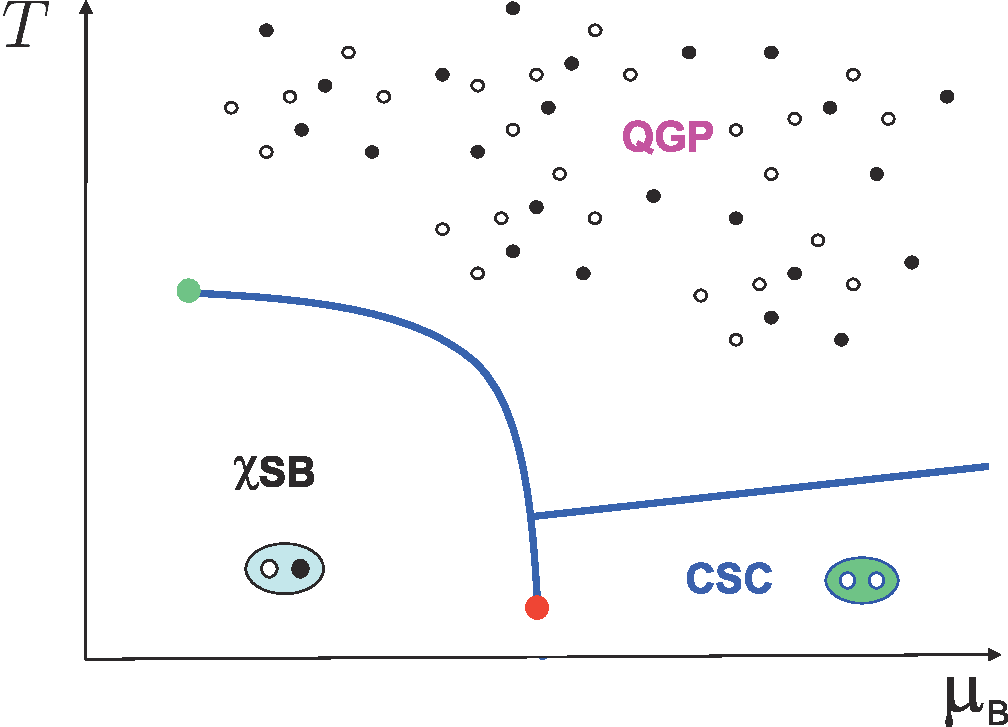
\includegraphics{Ch4_0702293.eps} }
% arXiv
\scalebox{0.40}{ 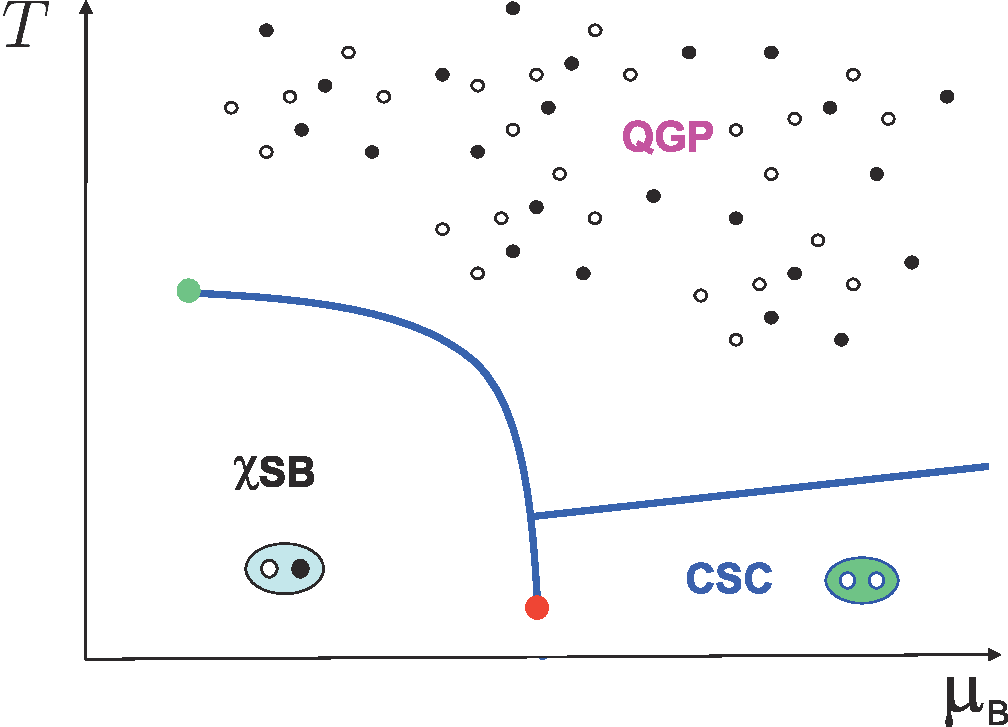
\includegraphics{Ch4_0702293.pdf} }
\vskip2mm
\caption{QCD phase diagram \cite{Hatsuda:2007rt}. The vertical axis represents temperature, and the horizontal axis represents the so-called ``baryon chemical potential," which is associated with the baryon number conservation (see footnote~\ref{fnote:chemical} in \sect{thermodynamics} for the use of the terminology chemical potential). In the figure, ``$\chi$SB" (which stands for chiral symmetry breaking) represents the hadron phase, and ``CSC" represents the so-called color superconducting phase. This is just a schematic diagram, and the full details of the phase diagram are still unclear; at this moment, it is not clear if there are any other phases in this diagram, and the boundaries of each phases are not clear either. 
%QCD�̑��} \cite{Hatsuda:2007rt}�D�c���͉��x�C�����̓o���I�����ۑ��ɔ������w�|�e���V�����i\sect{thermodynamics}�j�D����͖͎��}�ł���C�ق��̑��̑��݂̉”\���ɂ‚��Ă����̋��E�ɂ‚��Ă��C�킩���Ă��Ȃ����Ƃ�����
}
\label{fig:phase}
\end{figure}%
%%============


%%------------------
\subsection{Heavy-ion experiments}\label{sec:heavy_ion}
%%------------------

The quark-gluon plasma is a natural phenomenon from QCD. In fact, theoretically it has been known for a long time. But it was never formed in an experiment, let alone to measure physical properties. But in recent years, there exist \keyword{heavy-ion experiments} whose goals are to form QGP and to measure its physical properties. 
%�N�H�[�N�E�O���[�I���E�v���Y�}���̑��݂́C���_�I�ɂ͈ȑO����m���Ă����D�������C���̃v���Y�}�͎����őn��o���ꂽ���Ƃ��Ȃ��������̂ł���C�܂��Ă₻�̕����I�����ȂǑ���ꂽ���Ƃ͂Ȃ������D�������C�ߔN���̃v���Y�}���������ĕ����I�����𑪂낤�Ƃ���{\bf �d�C�I������}\index{���䂤�����񂵂�����@�d�C�I������}�����E�e�n�ł����Ȃ��Ă���D

Particle accelerators usually collide $e^+ e^-$, $pp$ or $p\bar{p}$, but the heavy-ion experiments collide heavy nuclei such as gold nuclei. Heavy atoms themselves are electrically neutral. In order to accelerate them, one has to strip electrons and to ionize them. So, such an experiment is called a heavy-ion experiment.
%�ʏ�̉�����ł́C�d�q�Ɨz�d�q�C�z�q�Ɣ��z�q�C���邢�͗z�q�ǂ������Փ˂����邪�C�d�C�I�������̑傫�ȓ����́C�����q�j�̂悤�ȏd�����q�j�ǂ������Փ˂�����_�ł���D�Ȃ��C���q���̂͒����Ȃ̂ŁC����������ɂ͓d�q���͂��Ƃ��ăC�I��������K�v������D���̂��߁C���̎�̎������d�C�I�������ƌ����D

One notable heavy-ion accelerator is the Relativistic Heavy Ion Collider (RHIC\index{RHIC}), which is located at Brookhaven National Laboratory and is in operation since 2000. Another heavy-ion experiment has been performed at CERN since 2010 using the Large Hadron Collider (LHC\index{LHC}). The plasma temperature by these colliders are estimated as about $2T_c$ at RHIC and about $5T_c$ at LHC.
%��\�I�ȏd�C�I�������Ƃ��ẮC2000�N����{�i�^�]���J�n���ꂽ�u���b�N�w�u�������������̑��Θ_�I�d�C�I���Փˌ^������ $\stackrel{\text{���b�N}}{\text{\bf RHIC}}$\index{RHIC@RHIC}�iRelativistic Heavy Ion Collider�j�ƌĂ΂���������g��������������D2010�N����́C�Z������{\bf LHC}\index{LHC@LHC}�iLarge Hadron Collider�j�ł��d�C�I�������������Ȃ��Ă���DRHIC�ł� $2T_c$�CLHC �ł� $5T_c$ ���x�̉��x�̃v���Y�}���B���ł���ƌ��ς����Ă���D

In heavy-ion experiments, one first collides heavy nuclei, and the plasma is formed if the temperature is high enough. But the plasma exists only transiently; the high temperature of the plasma causes it to expand, and then the plasma cools down by the expansion. In the end, the temperature is below the transition temperature, so quarks are confined into hadrons. What is observed is these secondary particles. The above history shows the difficulties of the experiment and its analysis:
%�d�C�I�������ł́C�܂��d���q�j���Փ˂��N�����C�\�������ł���΁C�����Z���ԃN�H�[�N�E�O���[�I���E�v���Y�}�����������D�������C���̃v���Y�}�͖c�����C�₦�Ă����D�ŏI�I�ɂ́C�]�ډ��x�ȉ��ɂȂ�n�h���������N�����D�ϑ������̂́C����瑽���̃n�h�����ł���D���̂��Ƃ���C�d�C�I�������̎�������щ�͂̓������������ɂȂ�F
\begin{itemize}

\item
The plasma has a very complicated time-evolution so that its analysis is not easy.
%�v���Y�}�����G�Ȏ��Ԕ��W������̂ŁC��͂͗e�Ղł͂Ȃ��D

\item
What is observed is not QGP itself but only its by-products such as hadrons. One has to infer what happened from the by-products. Thus, it is not an easy job to confirm even the QGP formation.
%�ϑ������̂̓v���Y�}���̂��̂ł͂Ȃ��D���Y���̃n�h�����Ȃǂł���C����畛�Y������k���ĉ����N�������˂��Ƃ߂Ȃ���΂����Ȃ��D���������āC���������v���Y�}�̐������N���������ǂ�����m��̂����e�Ղł͂Ȃ��D

\item
Many secondary particles are involved in the experiments. The purpose here is the QGP property as a thermal system, so one has to keep track of these particles as many as possible. 
%�����ɂ͑����̗��q���֗^����D�����ł̖ړI�͔M�͊w�n�Ƃ��Ẵv���Y�}�S�̂̐����Ȃ̂ŁC�ł���������Ȃ��������ꂽ���q��ǐՂ���K�v������D

\item
Finally, the perturbative QCD is not very effective for theoretical analysis as discussed below.
%�������C�ȉ��c�_����悤�ɗ��_�I�ȉ�͂̂����Őۓ��_���L���ł���ƍl�����Ȃ��D

\end{itemize}

%%------------------
\subsection{``Unexpected connection between string theory and RHIC collisions"}\label{sec:unexpected}
%%------------------

In 2005, the first detailed RHIC results were announced at the APS annual meeting. This press release has an interesting statement \cite{press}: ``The possibility of a connection between string theory and RHIC collisions is unexpected and exhilarating."%
\footnote{As far as I know, this is the first time string theory has been mentioned in the announcement of a major experiment. }
(Director of the DOE Office of Science) Here, ``string theory" meant the AdS/CFT duality. What is the ``unexpected connection" between string theory and RHIC collisions?
%2005 �N�CRHIC �̍ŏ��̂܂Ƃ܂����������ʂ��񍐂���C�}�X�R�~�ł��傫�Șb��ɂȂ����D���̃v���X�����[�X�ɂ́C�ꕗ�ς�����R�����g���ڂ��Ă��� \cite{press}�F�u�������_�� RHIC �����̊Ԃ̗\�����ʂ‚Ȃ���ɂ͐S��������D�v%
%\footnote{��^�����̃v���X�����[�X�Œ������_�����y���ꂽ�̂́C���ꂪ�j�㏉�������Ǝv����D}
%�����Ō����������_�Ƃ́CAdS/CFT�̂��Ƃ��w���D�����Ɋւ�����l�X������������AdS/CFT�� RHIC �����̗\�����ʂ‚Ȃ���Ƃ́C���̂��Ƃ��낤�H�@

In the RHIC announcement, it was stressed that \textit{quark-gluon-plasma does not behave like a free gas but behaves more like a perfect fluid}%
\footnote{Actually, the announcement stated that QGP behaves like a perfect ``liquid" to avoid the technical term ``fluid," but it was slightly misleading. See footnote~\ref{fnote:liquid} for more details.}.\index{perfect fluid} 
The difference between a free gas and a perfect fluid is that the latter has no viscosity. We will discuss the viscosity and hydrodynamics in \chap{hydro} in details, but let us remind you of freshman physics of viscosity. 
%RHIC �̔��\�ɂ��ƁC{\bf ���̃v���Y�}���u���z�C�́v�Ƃ��������ނ���u���S���́v\index{���񂹂��䂤����@���S����}�̂悤�ɐU��܂�}�Ƃ����_���������ꂽ�D���z�C�̂Ɗ��S���̂̈Ⴂ�́C��҂��S���������Ȃ��_�ł���D�S���◬�̗͊w�ɂ‚��ẮC\chap{hydro}�Ŗ{�i�I�Ɉ������C�����ł͔S���ɂ‚��ĊȒP�ɕ��K���Ă����D

%%============
\begin{figure}[tb]
\centering
%\hspace{0.25in}
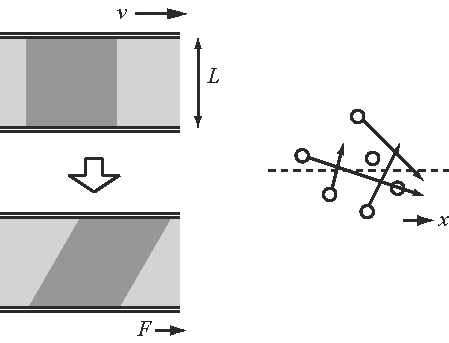
\includegraphics{Ch4_viscosity1_60.pdf}
\vskip2mm
\caption{\textit{Left}: when one moves the upper plate, the fluid is dragged due to the viscosity and the lower plate experiences a force. \textit{Right}: the close-up view of the fluid.
%��̔‚𓮂����ƁC�S���ɂ���ė��̑S�̂�����������D���̂��߉��̔‚ɂ��͂�������D�E�̐}�͗��̂̈ꕔ���g�債�����́D
}
\label{fig:viscosity}
\end{figure}%
%%============

As a simple example, consider a fluid between two plates and move the upper plate with velocity $v$ (\fig{viscosity}). As the fluid is dragged, the lower plate experiences a force. This force is the manifestation of the viscosity. In this case, the force the lower plate experiences per unit area $F/A$ is given by
\be
%
\boxeq{
\frac{F}{A}=\eta \frac{v}{L}~.
}
\label{eq:viscosity}
%
\ee
The proportionality constant $\eta$ is called the \keyword{shear viscosity}.
%����2�‚̔‚̊Ԃɗ��̂�����Ƃ��āC��̔‚𓮂����i\fig{viscosity}�j�D����ƁC���̑S�̂����������C���̔‚ɂ��͂�������D���̗͂����S���̌��ʂł���D���܂̏ꍇ�C���̔‚ɂ�����P�ʖʐς�����̗�$F/A$�́C��̔‚𓮂������x$v$�ɔ�Ⴕ�C���̂̌���$L$�ɔ���Ⴗ��F���W�� $\eta$ ��{\bf ����S����}\index{����˂񂹂����@����S����}�ƌĂ΂��D

Microscopically, the viscosity arises due to the momentum transfer between molecules. Figure~\ref{fig:viscosity}(right) shows a close-up view of the fluid and we put an artificial boundary to divide the fluid into two parts. The molecules collide with each other and are exchanged randomly through the boundary. But in the situation where we move the upper plate, the molecules in the upper-half part, on average, have more momentum in the $x$-direction than the ones in the lower-half part. These molecules are exchanged, which means that momentum in the $x$-direction is transported through the boundary. This is the microscopic origin of the viscosity.
%�����I�ɂ́C�S���͕��q�Ԃ̉^���ʂ̗A���ɂ���ċN���Ă���D\fig{viscosity}�i�E�j�͗��̂̈ꕔ���g�債�����̂ŁC�l�H�I�ɏ�̕����Ɖ��̕����ɕ��������̂��D���̂��\�����镪�q�݂͌��ɏՓ˂�����Ԃ��Ȃ���C�₦�����̋��E���s�������Ă���D�Ƃ���ŁC��̔‚𓮂����Ƃ������܂̏󋵂ł́C���ς���ƁC�㕔�̕��q�̕��������̕��q���$x$�����̉^���ʂ���葽�������Ă���D���̂悤�ȕ��q�����������Ƃ������Ƃ́C�‚܂�$x$�����̉^���ʂ����E���z���ėA������邱�Ƃ��Ӗ����Ă���D���ꂪ�S���̔����I�Ȍ����ł���D

The shear viscosity has units of 
$ [\eta] = \pascal\cdot\second = \kilogram\cdot\meter^{-1}\cdot\second^{-1} $
from \eq{viscosity}. Thus, one would expect from dimensional analysis that the shear viscosity is given by
%\eq{viscosity} ����킩��悤�ɁC����S������
%$ [\eta] = \pascal\cdot\second = \kilogram\cdot\meter^{-1}\cdot\second^{-1} $
%�̎��������D���������āC������͂��C
\be
%
\eta \simeq \rho \bar{v}l_\text{mfp}  \simeq \varepsilon \tau_\text{mfp}
\label{eq:viscosity_micro}
%
\ee
($\rho$: mass density, $\bar{v}$: mean velocity of particles, $l_{\rm mfp}$: mean-free path, $\varepsilon$: energy density, $\tau_\text{mfp}$: mean-free time).
Now, change the coupling constant. At strong coupling, the mean-free path becomes shorter. The viscosity arises due to the momentum transfer, and the transfer is less effective at strong coupling. So, the viscosity becomes smaller at strong coupling. In particular, a perfect fluid has no viscosity, so a perfect fluid is a strong coupling limit. This is somewhat confusing, but an ideal gas is the free limit, and a perfect fluid is the strong coupling limit%
\footnote{
The argument here has some limitations. First, the fluid must be a Newtonian fluid. [The Newtonian fluids are the fluids which satisfy \eq{viscosity}.] Second, among Newtonian fluids, we consider only the fluids where the momentum transfer occurs due to the mechanism described in the text. For example, ``honey" satisfies neither of these conditions. 

% added
This is an appropriate place to go back to the RHIC announcement of ``perfect liquid." In our discussion, the fluid is always gas-like and the momentum transfer is kinematic (\ie, the momentum is transferred by  particle motion), whereas in a liquid, the momentum transfer by potential energy among particles is more effective (see, \eg, Ref.~\cite{Csernai:2006zz}). What we have in mind is the strong coupling limit of the QGP gas. In this sense, saying that QGP is a perfect liquid is slightly misleading. But in the strong coupling limit, the distinction between a gas and a liquid becomes rather subtle.
\label{fnote:liquid}
%The discussion here has 2 limitations. First, the argument is true only for  Newtonian fluids. [The Newtonian fluids are the fluids which satisfy \eq{newtonian}.] Second, the argument is true only if the momentum transfer occurs due to the mechanism described in the text. For example, ``honey" satisfies neither of these conditions.
}.
%�ƂȂ邱�Ƃ����҂����i$\rho$�F���ʖ��x�C $\bar{v}$�F���̂��\�����闱�q�̕��ϑ��x�C $l_\text{mfp}$�F���ώ��R�s���C$\varepsilon$�F�G�l���M�[���x�C$\tau_\text{mfp}$�F���ώ��R���ԁj�D���ꂩ���‚킩�邱�Ƃ́C���ݍ�p�ƔS���̊֌W�ł���D���ݍ�p�������Ȃ�ƁC���ώ��R�s���͒Z���Ȃ�D�S���͉^���ʂ̗A���ɂ���ċN���������C���ݍ�p�������ƗA�����W�����邽�߂ł���D�����瑊�ݍ�p��������΁C�S���͏������Ȃ�D�Ƃ��Ɋ��S���͔̂S���������Ȃ��̂ŁC����͑��ݍ�p���ɒ[�ɋ������Ƃ���������D���̓_��������킵�����C���z�C�̂͑��ݍ�p���Ȃ��Ɍ��ł���C�t�Ɋ��S���̂͑��ݍ�p�������Ɍ��ł���%
%\footnote{
%�ȏ�̋c�_�́C���̈�ʂɐ��藧�‚��̂ł͂Ȃ��D(a) \eq{viscosity} �𖞂������́i�j���[�g�����́j�C����(b) �{���ɂ���悤�ȕ��@�ʼn^���ʗA�����N���闬�̂Ɍ�����D���Ƃ��΃n�`�~�c�͂ǂ���̉�����������Ȃ��D}�D

A small viscosity implies the strong interaction. According to RHIC, QGP has a small viscosity, so this implies that QGP is strongly-coupled. This is an interesting discovery, but then how can one study such a strong coupling problem theoretically? One cannot rely on the perturbative QCD. This is one main obstacles in the QGP research. String theory may be a good place to study such an issue. It turns out that the prediction of the shear viscosity using AdS/CFT is close to the RHIC result (\chap{QGP}). This is the ``unexpected connection" the RHIC announcement meant.
%���̂悤�ɏ����ȔS���́C���ݍ�p�����������Ă��邱�Ƃ���������DRHIC�̔��\�ɂ��ƁCQGP�͏����ȔS�������‚Ƃ������ƂȂ̂ŁCQCD�̑��ݍ�p�͂܂����������Ă��邱�ƂɂȂ�D�����Ƃ������Ȃ�ƁCQGP�̐����𗝘_�I�ɋc�_�������Ă��CQCD�̐ۓ��_���g���킯�ɂ͂����Ȃ��D���ꂪQGP�����̂�������ȓ_�ł���D�����œo�ꂷ��̂�AdS/CFT�ł���DRHIC�����̌��ʂ́CAdS/CFT���g��������S�����̗\���Ƌ߂����Ƃ����������̂ł���i\chap{QGP}�j�D���ꂪ�u�\�����ʂ‚Ȃ���v�ł���D

We will further discuss heavy-ion experiments and their results in \sect{QGP}.
%�d�C�I�������Ƃ��̌��ʂɂ‚��ẮC\sect{QGP}�ł���ɋc�_����D

%%%%%%%%%%%%%%%%%%%%%%
\section{Large-$N_c$ gauge theory
%���[�W$N_c$�Q�[�W���_
}\label{sec:large_N}
%%%%%%%%%%%%%%%%%%%%%%

In QCD, the perturbation theory has a limited power, and it is still difficult to solve QCD nonperturbatively. An approximation method, the so-called \keyword{large-$N_c$ gauge theory}, was proposed by 't~Hooft, and this idea is naturally related to string theory \cite{'tHooft:1973jz}%
\footnote{See Chap.~8 of Ref.~\cite{coleman} for the details of the large-$N_c$ gauge theory.}.
%QCD�͐ۓ��_�̎g����̈悪�����Ă���C���܂���QCD���ۓ��_�I�ɉ����͍̂���ł���D���̂��ߋߎ���@�Ƃ��Ē�Ă��ꂽ�̂��C�g�z�[�t�g��{\bf ���[�W$\boldsymbol{N_c}$�Q�[�W���_}\index{��[��N���[������@���[�W$N_c$�Q�[�W���_}�Ƃ����l���ł��� \cite{'tHooft:1973jz} �D�����āC���̍l���������_�Ɗ֌W����D

There are three colors in QCD, but in the large-$N_c$ gauge theory, one considers a large number of colors. For example, consider a $U(N_c)$ gauge theory. The gauge field is written as an $N_c \times N_c$ matrix,  
% corrected/modified
$(A_\mu)_i^{~j}$.
%QCD�ł̓J���[�̎��R�x��3�����C���[�W$N_c$�Q�[�W���_�ł̓J���[�̐�$N_c$���傫���ꍇ���l����D���Ƃ��΁C���z�I�� $U(N_c)$�Q�[�W���_���l����D���̏ꍇ�C�Q�[�W�� $(A_\mu)^i_{~j}$ ��$N_c \times N_c$ �s��ł���킳���D

%SU(N) �g���[�X���X�E�G���~�[�g
%U(N) �G���~�[�g
Then, the theory has two parameters,
\begin{center}
%
gauge theory coupling constant $g_\text{YM}$, \qquad number of colors $N_c$~.
%
\end{center}
Instead, we will use $N_c$ and the \textit{'t~Hooft coupling}\index{t~Hooft coupling@'t~Hooft coupling} $\lambda := g_{\rm YM}^2 N_c$ as independent parameters. The \keyword{large-$N_c$ limit} is given by%
\footnote{If one recovers $g_\text{YM}$, the limit implies $g_\text{YM}\rightarrow0$.}
\begin{center}
%
$N_c\rightarrow\infty$ while $\lambda$ is kept fixed and large.
%
\end{center}
This is a nontrivial limit as we will see. Namely, the theory does not reduce to the free one in this limit because the effective coupling is given by $\lambda$. Thus, $\lambda\gg1$ is a strong coupling limit. 
%���������āC���̗��_�ɂ�2�‚̃p�����[�^�����邱�ƂɂȂ�F
%\begin{center}
%
%�Q�[�W���_�̌����萔 $g_\text{YM}$ �C\qquad �J���[�̐� $N_c$~.
%
%\end{center}
%�ȉ��ł́C�Ɨ��ȃp�����[�^�Ƃ��āC������ $N_c$ ��{\bf �g�z�[�t�g�����萔}\index{�Ƃف[�ӂƂ��‚����Ă�����@�g�z�[�t�g�����萔}$\lambda := g_{\rm YM}^2 N_c$ ���g���D�����ŁC
%\begin{center}
%
%$\lambda$ ��傫�Ȓl�ɌŒ肵�‚C$N_c\rightarrow\infty$
%
%\end{center}
%�Ƃ����Ɍ����Ƃ鑀���{\bf ���[�W$\boldsymbol{N_c}$ �Ɍ�}\index{��[��N���悭����@���[�W$N_c$�Ɍ�}�ƌ���%
%\footnote{$g_\text{YM}$�𕜊�������ƁC$g_\text{YM}\rightarrow0$���Ӗ�����D}�D
%�ȉ��݂�悤�ɁC����̓m���g���r�A���ȋɌ��ł���D�‚܂�C���̋Ɍ��ŗ��_�͎��R��ɂ͋A�����Ȃ��D���́C�L�������萔��$\lambda$�ł���킳��邩��ł���D���������āC$\lambda\gg1$ �̂Ƃ��́C�ނ��닭�����Ɍ��ł���D

The large-$N$ limit of, \eg, $O(N)$ vector model often appears in condensed-matter physics. The large-$N_c$ gauge theory has the same spirit but has important differences. The vector model is solvable in this limit, but the gauge theory is hard to solve even in this limit. Also, the vector model essentially reduces to a classical theory. The gauge theory also reduces to a classical theory, but this classical theory is a \textit{classical gravitational theory} as we will see in a moment. 
%�����Ȃǂł́C���΂���$O(N)$�x�N�g���͌^�̃��[�W$N$�Ɍ����l����D���[�W$N_c$�Q�[�W���_���l�����͓����ł��邪�C�傫�ȈႢ������D�x�N�g���͌^�͂��̋Ɍ��ʼn����邪�C�Q�[�W���_�͂��̋Ɍ��ł������͓̂���D���[�W$N$�ł́C�x�N�g���͌^�͖{���I�ɌÓT�_�ɋA������D�Q�[�W���_���ÓT�_�ɂ͋A�����邪�C�ȉ��ł݂�悤�ɂ���͌ÓT�_�ƌ����Ă��ÓT�d�͗��_�ł���D

%%============
\begin{figure}[tb]
\centering
\scalebox{0.75}{ 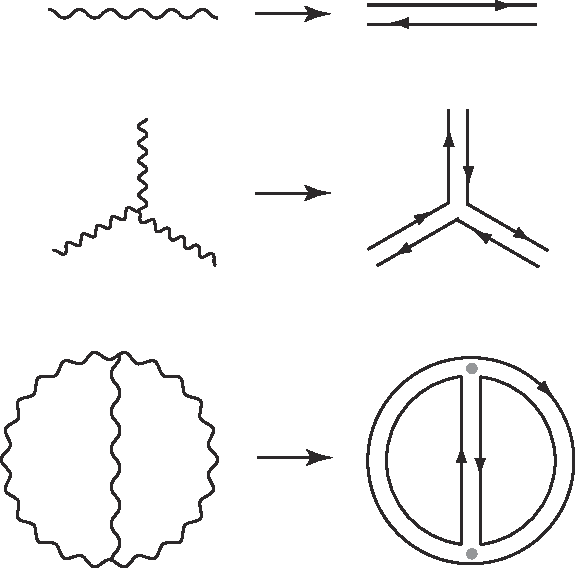
\includegraphics{Ch4_double_line.pdf} }
\vskip2mm
\caption{The propagator of the gauge field (wavy lines) and the interaction vertex by double-line notations (top, middle). The bottom figure is an example of vacuum amplitudes.
%�Q�[�W��̃v���p�Q�[�^�[�i�g���j�Ƒ��ݍ�p�̒��_�� double-line notation �ŕ`�������́i��C���j�ƁC�^��_�C�A�O�����̈��i���}�j�D
}
\label{fig:double-line-notation}
\end{figure}%
%%============

In Feynman diagrams, a gauge theory propagator is represented by a single line. But to keep track of colors, it is convenient to use the ``double-line notation," \index{double-line notation} where the propagator is represented by a double-line with opposite arrows (\fig{double-line-notation}). Then, draw diagrams so that the direction of arrows is preserved. As far as color indices are concerned, the gauge field behaves as a quark-antiquark pair, so one can regard the double-line as the pair. Namely, one line represents the rows of the matrix $(A_\mu)^i_{~j}$, and the other represents the columns. 
%�t�@�C���}���E�_�C�A�O�����ł́C�Q�[�W��̃v���p�Q�[�^�[����{�̐��ł���킷���C�J���[�̎��R�x�����₷�����邽�߂ɁC\fig{double-line-notation}�̂悤�ɖ��‚��̓�d���ŏ����̂��֗��ł���i``double-line notation"�j�D�����āC�S�̂Ƃ��Ė��̌������ۂ����悤�Ƀ_�C�A�O�����������D�J���[�̓Y���Ɋւ������C�Q�[�W��̓N�H�[�N�E���N�H�[�N�̂悤�ɐU��܂��̂ŁC��d�����N�H�[�N�E���N�H�[�N�Ƃ݂Ȃ����Ƃ��ł���D�‚܂�C�Е��̐����s��  $(A_\mu)^i_{~j}$  �̍s�C�����Е����������킵�Ă���D

Or, in string theory context, a double-line represents the propagation of an open string because an open string represents a gauge field (\chap{string}). A double-line corresponds to the endpoints of a string%
\footnote{We will encounter string theory again in the large-$N_c$ limit below, but this string is not the same as the open string here. String theory appeared below is a closed string theory. }.
%�܂��́C�����_�̕����ł́C����͊J�����`�����Ă���l�q�ɂق��Ȃ�Ȃ��i\chap{string}�j�D��d�����J���̒[�Ȃ̂ł���D�J���́C�Q�[�W�������킷����ł���%
%\footnote{�ȉ��C���[�W $N_c$ �Ɍ��ł܂������_���o�ꂷ�邪�C���̊J���ƈȉ��œo�ꂷ�錷���_�́C�������̂ł͂Ȃ��D�ȉ��œo�ꂷ�錷���_�́C�Œ��̗��_������ł���D}�D

The Lagrangian of a gauge field is schematically written as
%�Q�[�W��̃��O�����W�A���́C�`���I��
\be
%
{\cal L} = \frac{1}{g_\text{YM}^2} \{ \del A \del A+ A^2 \del A + A^4 \}
= \frac{N_c}{\lambda} \{ \cdots \}~.
%\label{eq:}
%
\ee
%��p�́C $A \rightarrow iU\del U^{-1}+UAU^{-1}$ �Ƃ����ϊ��̉��ŕs�ςł���i$U \in U(N_c)$�j�D
From the Lagrangian, one can derive Feynman rules to obtain amplitudes. Here is the summary of rules:
%���̂悤�ȃ��O�����W�A������C��̗��_���g���ĐU�������߂邽�߂̃t�@�C���}���E���[���������邪�C���[���������܂Ƃ߂�ƈȉ��̂悤�ɂȂ�F
\begin{itemize}

%\item
%�Q�[�W��̃v���p�Q�[�^�[����‚��̓�d���ŏ����D�i``double-line notation"�j�D�e�����s��́u�Y���v������킵�C�S�̂Ƃ��Ė��̌������ۂ����悤�Ƀ_�C�A�O�����������D

\item
Associate the factor $\lambda/N_c$ for each propagator.
%�v���p�Q�[�^�[�ɂ́C$\lambda/N_c$ �̈��q��t�^����D

\item
Associate the factor $N_c/\lambda$ for each interaction vertex%
\footnote{In \fig{diagram}, the vertex is represented by a gray dot. Below we will take care only of the factors $N_c$ and $\lambda$ in diagrams, and we will discuss only ``vacuum amplitudes" with no external lines.}.
%���ݍ�p������킷�u���_�v%\footnote{\fig{diagram}�ł̓O���[�̊ۂł���킵���D�Ȃ��C�ȉ��ł̓_�C�A�O������ $\lambda$ �� $N_c$ �̈��q�����ɒ��ӂ��C�u�O���v�������Ȃ��u�^��_�C�A�O�����v�������l����D}�ɂ́C$N_c/\lambda$ �̈��q�D

\item
Associate the factor $N_c$ for each loop (because of the summation over $N_c$ colors).
%�u���[�v�v�ɂ� $N_c$ �̈��q�i$N_c$ �̎��R�x�����邽�߁j�D

\end{itemize}
Denote the number of vertices as $V$, the number of propagators as $E$, and the number of loops as $F$. From the Feynman rules, one gets
%���̂��߁C���_�̐���$V$�C�v���p�Q�[�^�[�̐���$E$�C���[�v�̐���$F$�Ƃ���ƁC
\be
%
\left( \frac{N_c}{\lambda} \right)^V
\left( \frac{\lambda}{N_c} \right)^E N_c^F 
%
= \lambda^{E-V} N_c^{V-E+F}~.
\label{eq:N_counting}
%
\ee
For example, the diagram~\ref{fig:diagram}(a) has $(V, E, F) = (2,3,3)$, so
%�ƂȂ�D���Ƃ��΁C\fig{diagram}(a) �̃_�C�A�O������$(V, E, F) = (2,3,3)$�Ȃ̂�
\be
%
\left( \frac{N_c}{\lambda} \right)^2
\left( \frac{\lambda}{N_c} \right)^3 N_c^3
= \lambda N_c^2~.
%\label{eq:}
%
\ee
The diagram~\ref{fig:diagram}(b) has $(V, E, F) = (4,6,4)$, so
%\fig{diagram}(b) �̃_�C�A�O������$(V, E, F) = (4,6,4)$�Ȃ̂�
\be
%
\left( \frac{N_c}{\lambda} \right)^4
\left( \frac{\lambda}{N_c} \right)^6 N_c^4
= \lambda^2 N_c^2~.
%\label{eq:}
%
\ee
Thus, these results are summarized schematically as
%���������āC�����̃_�C�A�O�����͌`���I��
\be
%
(1+\lambda+\lambda^2+\cdots) N_c^2 
= f_0(\lambda) N_c^2~.
\label{eq:planar}
%
\ee
%�Ƃ����`�ɂ܂Ƃ܂�D

But it is not always the case that diagrams take the form \eqref{eq:planar}. For example, the diagram~\ref{fig:diagram}(c) has $(V, E, F) = (4,6,2)$, so
%�������C�_�C�A�O�����͂��‚�\eq{planar}�̌`���Ƃ�킯�ł͂Ȃ��D���Ƃ��΁C\fig{diagram}(c) �̃_�C�A�O������$(V, E, F) = (4,6,2)$�Ȃ̂�
\be
%
\left( \frac{N_c}{\lambda} \right)^4
\left( \frac{\lambda}{N_c} \right)^6 N_c^2
= \lambda^2~.
%\label{eq:}
%
\ee
The diagrams such as \fig{diagram}(a), (b) are called \keyword{planar}, and the diagrams such as \fig{diagram}(c) are called \keyword{non-planar}. The word ``planar" (``non-planar")  means that one can (cannot) draw the diagrams on a plane. Including non-planar diagrams, the diagrams are written as
%�ƂȂ�D\fig{diagram}(a), (b) �̂悤�ȃ_�C�A�O������{\bf �v���i�[}\index{�ӂ�ȁ[�����������@�v���i�[�E�_�C�A�O����}�iplanar�j�ƌ����C\fig{diagram}(c) �̂悤�ȃ_�C�A�O������{\bf ��v���i�[}\index{�Ђӂ�ȁ[�����������@��v���i�[�E�_�C�A�O����}�inon-planar�j�ƌ����D�v���i�[�i��v���i�[�j�Ƃ́C���ʏ�ɏ�����i�����Ȃ��j�Ƃ����Ӗ��ł���D��v���i�[�E�_�C�A�O�������܂߂�ƁC�_�C�A�O������
\be
%
f_0(\lambda) N_c^2 + f_1(\lambda) N_c^0 + f_2(\lambda) \frac{1}{N_c^2} + \cdots~.
\label{eq:planar&nonplanar}
%
\ee
In the large-$N_c$ limit, the first term of \eq{planar&nonplanar}, the planar diagrams, dominate.
%�Ƃ����`�ɂ܂Ƃ܂�D���[�W $N_c$ �Ɍ��ł́C\eq{planar&nonplanar} �̑�1���C�v���i�[�E�_�C�A�O�������x�z�I�ɂȂ�D

%%============
\begin{figure*}[tb]
\centering
\scalebox{0.75}{ 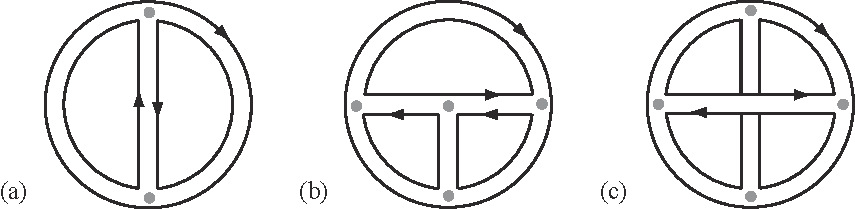
\includegraphics{Ch4_diagram.pdf} }
\vskip2mm
\caption{Examples of vacuum amplitudes. Fig.~(a) and (b) are planar diagrams, and (c) is a non-planar diagram.
%�^��_�C�A�O�����̗�D(a), (b) �̓v���i�[�E�_�C�A�O�����ŁC(c) �͔�v���i�[�E�_�C�A�O�����D
}
\label{fig:diagram}
\end{figure*}%
%%============

%%============
\begin{figure}[tb]
\centering
%\hspace{0.25in}
\scalebox{0.75}{ 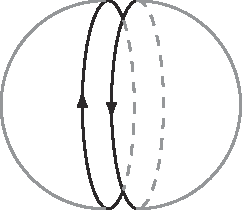
\includegraphics{Ch4_surface.pdf} }
\vskip2mm
\caption{Relation between a diagram and a two-dimensional surface.
%�_�C�A�O������2�����ʂ̊֌W�D
}
\label{fig:surface}
\end{figure}%
%%============

Whether diagrams dominate in the large-$N_c$ limit depends on whether one can draw them on a plane (or a sphere). This strongly suggests the relation between the diagrams and topology. In fact, one can draw the diagram~\ref{fig:diagram}(c) on a torus%
\footnote{This is beyond my ability to draw such an illustration. Anyway, such an illustration is hard to see. I recommend readers to draw such an illustration on their own or to draw diagrams on an object with a handle (such as a doughnut or a mug).}.
%�_�C�A�O���������ʏ�i���邢�͋��ʏ�j�ɏ����邩�ǂ����ŁC���[�W $N_c$ �Ɍ��Ŏx�z�I�ɂȂ邩�ǂ��������܂�Ƃ����̂́C�_�C�A�O�����ƃg�|���W�[�̊֌W����������D���ہC\fig{diagram}(c) �̓g�[���X��ɂ͏������Ƃ��ł���%\footnote{������G�ɕ`���̂́C�M�҂̉�͂ɗ]�邵�C���ɂ����G�ɂȂ邾���ł���D�ǎҎ��炪�G��`���Ă݂邩�C���ۂɃn���h�������•��̏�Ƀ_�C�A�O������`���Ă݂�̂������D}�D

In general, one can understand the relation between these diagrams and topology in the following way. Let us fill in loops with surfaces. One can construct a closed two-dimensional surface (\fig{surface}). Each propagator is an edge of the surface (polygon), and each vertex is a vertex of the polygon. Then, one can regard the number of propagators $E$ as the number of edges, and the number of loops $F$ as the number of faces of the polygons. Now, in this interpretation, the power of $N_c$ in \eq{N_counting} is the Euler characteristic $\chi$, which is a topological invariant: 
%��ʂɂ͎��̂悤�ɍl����D���܁C�v���p�Q�[�^�[��ӂƂ��āC���[�v��ʂŖ��߂�ƁC2�����ʂ��ł���i\fig{surface}�j�D�‚܂�C2�����ʂ��i���_�Ō����j�ӂŕ��������}�`���ł���D�����l�����ꍇ�C�v���p�Q�[�^�[�̐� $E$�C���[�v�̐� $F$ �́C���ꂼ��2�����ʂ̕ӂ̐��C�ʂ̐��Ƃ����Ӗ������D�������C2�����ʂƂ��Ă݂��ꍇ�C\eq{N_counting}�ɂ������$N_c$�̃x�L�̓I�C���[�W�� $\chi$�ł���C�g�|���W�J���s�ϗʂł���F
% ���FEuler characteristic �u�I�C���[���v�Ƃ͕ʕ�
\be
%
\chi = V-E+F~.
%= 2-2H-B
%= 2-2g
%\label{eq:}
%
\ee
%�i$H$�F�n���h���̐��C$g$�F�W�[�i�X�j
%�i$H$�F�n���h���̐��C$B$�F���E�̐��C$g$�F�W�[�i�X�j
For example, a sphere has $\chi=2$, and a torus has $\chi=0$. If we denote the number of handles (genus) as $h$, one can also write $\chi=2-2h$. Namely, the planar diagram \fig{diagram}(a),(b) correspond to the sphere, and the non-planar diagram \fig{diagram}(c) corresponds to the torus (\fig{topology}).
%���Ƃ��΁C���� $\chi=2$�C�g�[���X�� $\chi=0$�ł���D�n���h���̐��i�W�[�i�X�j�� $h$ �Ƃ���ƁC$\chi=2-2h$ �Ə������Ƃ��ł���D
%�W�[�i�X�C�퐔
%�����Â��”\�ȕ‹Ȗʂ̏ꍇ

%%============
\begin{figure}[tb]
\centering
%\hspace{0.25in}
\scalebox{0.75}{ 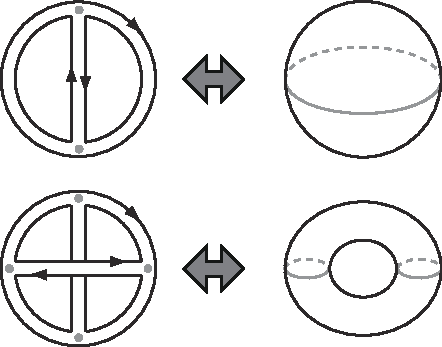
\includegraphics{Ch4_topology_75.pdf} }
\vskip2mm
\caption{Diagrams and topology.}
\label{fig:topology}
\end{figure}%
%%============

Now, the summation of vacuum diagrams is a partition function, so the partition function is given by
%�^��_�C�A�O�����̑��������͕��z�֐��Ȃ̂ŁC
\be
%
\ln Z_\text{gauge} = \sum_{h=0}^\infty N_c^{\chi} f_h (\lambda)
\label{eq:partition_gauge}
%
\ee
or
%�ƂȂ�D
%���������āC
\begin{center}
\fbox{
\begin{tabular}{l}
Second clue of AdS/CFT: \\
The partition function of a large-$\Nc$ theory is given by \\
a summation over the topologies of two-dimensional surfaces.
%���[�W$N_c$�Ɍ��ł́C���z�֐���2�����ʂ�\\�g�|���W�[�̑��������Ƃ��Ă���킳���D
\end{tabular}
}
\end{center}

As one can see from \fig{diagram}(a), (b), the more propagators we have, the more dominant a diagram is in the large-$N_c$ limit. This limit is hard to evaluate in a field theory. On the other hand, the two-dimensional surface point of view becomes better in this limit. The diagrams become denser in this limit, and they approach a smoother two-dimensional surface.
%\fig{diagram}(a), (b)���ׂĂ킩��悤�ɁC�v���p�Q�[�^�[�������قǁC���[�W $\lambda$ �Ŏx�z�I�ɂȂ�D���̋Ɍ��͏�̗��_�I�ɂ͕]��������D����C���̋Ɍ��Ńv���p�Q�[�^�[�͂܂��܂����ɂȂ�C�Ȃ߂炩��2�����ʂɂ��߂Â��Ɗ��҂����D

In the next chapter, we will see that the perturbative expansion of string theory is also given by a summation over two-dimensional topologies (\fig{string_amplitude}). This ``coincidence" leads one to guess that two theories, gauge theory and string theory, are actually equivalent: 
%���͂ŏڂ����������邪�C���͌����_�̐ۓ��W�J���C2�����ʂ̃g�|���W�[�̑��������Ƃ��Ă���킳���i\fig{string_amplitude}�j�D���������āC����2�‚̗��_�͓����ł���C2�‚̕��z�֐����������ƍl������F
\be
%
Z_\text{gauge} = Z_\text{string}~.
%\label{eq:}
%
\ee
In particular, a summation of two-dimensional closed surfaces corresponds to the gravitational perturbative expansion. There, the sphere, the planar diagrams, corresponds to classical gravity, and the torus, one of non-planar diagrams, corresponds to gravity at one-loop. In \sect{BH_entropy}, the holographic principle gives the first clue for AdS/CFT, and the large-$N_c$ gauge theory gives us the second clue.  
%�Ƃ��ɁC�‚���2�����ʂ̑��������́C�d�͂̐ۓ��W�J�ɑ������C�v���i�[�E�_�C�A�O�����̋��͌ÓT�d�́C��v���i�[�E�_�C�A�O�����̃g�[���X�͏d�͂�1���[�v�ɑ�������D

%���ꂪAdS/CFT�ւ̑����ł���D

%%%%%%%%%
\section{\titlesummary}%\label{sec:}
%%%%%%%%%

\begin{itemize}
\item 
According to heavy-ion experiments, QGP behaves as a perfect fluid with a very small shear viscosity. This implies that QGP is strongly-coupled.
\item 
It is difficult to compute gauge theories such as QCD at strong coupling. The large-$\Nc$ gauge theory provides an approximation to compute a strong coupling limit.
\item 
The partition function of a large-$\Nc$ theory is given by 
a summation over the topologies of two-dimensional surfaces.
\end{itemize}

%%------------------
\titlenewterms
%%------------------

\begin{multicols}{2}
\noindent
quarks\\
quantum chromodynamics (QCD)\\
gluons\\
fundamental/adjoint representation\\
color\\
flavor\\
%adjoint representation\\
asymptotic freedom\\
hadrons\\
color confinement\\
Debye screening\\
quark-gluon plasma (QGP)\\
heavy-ion experiments\\
%RHIC\\
%LHC\\
perfect fluid\\
shear viscosity\\
%large-$N_c$ gauge theory\\
't~Hooft coupling\\
large-$N_c$ limit\\
double-line notation\\
planar/non-planar\\
topology
\end{multicols}

%%%%%%%%%
\section{Appendix: Review of gauge theory}\label{sec:YM}
%%%%%%%%%

\newcommand{\Am}{A_\mu}

%%%
\head{$U(1)$ gauge theory}
%%%

First, recall a $U(1)$ gauge theory. Consider a complex scalar field:
\be
%
\calL = - \del_\mu \phi^* \del^\mu \phi -m^2 \phi^*\phi~.
%\label{eq:}
%
\ee
The theory is invariant under the global $U(1)$ transformation
\be
%
\phi \rightarrow U \phi~, \quad (U:= e^{i\alpha})~.
%\label{eq:}
%
\ee
The theory is not invariant under the local $U(1)$ transformation though:
\be
%
\phi \rightarrow U(x) \phi~.
%\label{eq:}
%
\ee
The local symmetry can be incorporated by introducing a $U(1)$ gauge field $\Am$ and the covariant derivative $D_\mu$:
\be
%
D_\mu \phi = (\del_\mu - i\Am)\phi~,
%\label{eq:}
%
\ee
where $\Am$ transforms as 
\be
%
\Am \rightarrow \Am + \del_\mu \alpha = \Am - i(\del_\mu U)U^{-1}~.
%\label{eq:}
%
\ee
The covariant derivative transforms as 
\be
%
D_\mu \phi \rightarrow U D_\mu \phi~, 
\quad \text{or} \quad
D_\mu \rightarrow U D_\mu U^{-1}~.
%\label{eq:}
%
\ee

One makes the invariant action using covariant (or invariant) quantities such as $D_\mu\phi$ and $F_{\mu\nu} = \del_\mu A_\nu - \del_\nu A_\mu$. The gauge field action is given by
\be
%
\calL = - \frac{1}{4e^2} F^{\mu\nu}F_{\mu\nu}~.
%\label{eq:}
%
\ee
We normalized the gauge field so that the charge $e$ (coupling constant) appears only as the overall normalization. The usual form is obtained by
\be
%
\Am \rightarrow e \Am~.
%\label{eq:}
%
\ee
Then, the transformation law and the covariant derivative become
\begin{align}
%
\Am & \rightarrow \Am + \frac{1}{e}\del_\mu \alpha~,\\
D_\mu \phi &= (\del_\mu - ie\Am)\phi~.
%\label{eq:}
%
\end{align}

%%%
\head{$U(\Nc)$ gauge theory}
%%%

Now, let us consider a scalar field with $\Nc$ components $\phi_i = (\phi_1, \phi_2, \cdots)$. Consider the Lagrangian given by
\be
%
\calL = - (\del_\mu \phi)^\dag (\del^\mu \phi) -m^2 \phi^\dag\phi~.
%\label{eq:}
%
\ee
The theory has a global $U(\Nc)$ symmetry:
\be
%
\phi_i \rightarrow U_i^{~j} \phi_j~,
%\label{eq:}
%
\ee
where $U$ is a unitary $\Nc\times\Nc$ matrix. Again, one can promote the symmetry to a local symmetry by  introducing a gauge field $\Am$ and the covariant derivative $D_\mu$ for $\phi$:
\be
%
D_\mu \phi = (\del_\mu - i\Am)\phi~,
%\label{eq:}
%
\ee
where $\Am$ is a Hermitian $\Nc\times\Nc$ matrix $(\Am)_i^{~j}$ and transforms as 
\be
%
\Am \rightarrow U \Am U^{-1} - i(\del_\mu U)U^{-1}~.
\label{eq:A_transf}
%
\ee
Then, the covariant derivative transforms as 
\begin{align}
%
D_\mu \phi &\rightarrow (\del_\mu U) \phi + U\del_\mu \phi 
- i\{ U \Am U^{-1} - i(\del_\mu U)U^{-1} \} U \phi \\
&= U (\del_\mu - i\Am) \phi~,
%\label{eq:}
%
\end{align}
so
\be
%
D_\mu \phi \rightarrow U D_\mu \phi~, 
\quad \text{or} \quad
D_\mu \rightarrow U D_\mu U^{-1}~.
%\label{eq:}
%
\ee

%One calls that the field $\phi_i$ belongs the fundamental representation of the gauge group. So far, we consider a matter in the fundamental representation, but matter fields in the adjoint representation often appear in AdS/CFT. An adjoint scalar $(\phi_A)_i^{~j}$ transforms as
So far, we consider the matter field $\phi_i$, a field in the fundamental representation, but matter fields in the adjoint representation often appear in AdS/CFT. An adjoint scalar $(\phi_A)_i^{~j}$ transforms as
\be
%
\phi \rightarrow U\phi_A U^{-1}~.
%\label{eq:}
%
\ee
Namely, it transforms as $\phi_i (\phi^\dag)^j$. The gauge field $(\Am)_i^{~j}$ also belongs to the adjoint representation although $\Am$ transformation \eqref{eq:A_transf} itself has an inhomogeneous term $(\del_\mu U)U^{-1}$. The definition of the covariant derivative depends on the fields it acts. Following the same procedure as $\phi_i$, one can show that the covariant derivative of $\phi_A$ is given by
\be
%
D_\mu \phi_A = \del_\mu \phi_A - i [\Am,\phi_A]~.
%\label{eq:}
%
\ee

One can show
\be
%
[D_\mu, D_\nu]\phi = \left\{ \del_\mu A_\nu - \del_\nu A_\mu - i [A_\mu, A_\nu] \right\} \phi~.
%\label{eq:}
%
\ee
Note that $D_\mu$ is a differential operator, but its commutator is no longer a differential operator. So, we define the field strength as
\be
%
F_{\mu\nu} =  -i[D_\mu, D_\nu] = \del_\mu A_\nu - \del_\nu A_\mu - i [A_\mu, A_\nu]~.
%\label{eq:}
%
\ee
Because $D_\mu \rightarrow U D_\mu U^{-1}$, $F_{\mu\nu}$ transforms as
\be
%
F_{\mu\nu} \rightarrow U F_{\mu\nu} U^{-1}~.
%\label{eq:}
%
\ee
In the $U(1)$ gauge theory, $F_{\mu\nu}$ is invariant, but here $F_{\mu\nu}$ is covariant. We define the gauge theory action as
\be
%
\calL = - \frac{1}{2g_\text{YM}^2} \text{tr} (F^{\mu\nu}F_{\mu\nu})~.
%\label{eq:}
%
\ee

Write the transformation matrix $U$ as
\begin{align}
%
U &= e^{iH}~, \\
H &= \alpha \cdot 1 + \alpha^a t^a~. \quad (a=1,\ldots, \Nc^2-1)
%\label{eq:}
%
\end{align}
The parameter $\alpha$ represents $U(1)$ transformation, and the parameters $\alpha^a$ represent $SU(\Nc)$ transformations. The matrices $t^a$ are called $SU(\Nc)$ generators. Because $U$ is a unitary matrix, $t^a$ are traceless Hermitian matrices. In general, the generators satisfy the commutation relation
\be
%
\left[ t^a, t^b \right] = if_{abc} t^c~,
%\label{eq:}
%
\ee
where $f_{abc}$ is called the structure constant of the gauge group. We normalize the generators so that
\be
%
\text{tr}\left( t^a t^b \right) = \frac{1}{2} \delta^{ab}~.
%\label{eq:}
%
\ee
Using $t^a$, one can decompose matrix fields such as $\Am$ and $F_{\mu\nu}$, \eg, 
\be
%
(\Am)_i^{~j} = \Am^a (t^a)_i^{~j}~.
%\label{eq:}
%
\ee
Then, the action becomes
\be
%
\calL = - \frac{1}{2g_\text{YM}^2} \text{tr} (F^{\mu\nu}F_{\mu\nu})
= - \frac{1}{4g_\text{YM}^2} F^{a\mu\nu}F^a_{\mu\nu}~.
%\label{eq:}
%
\ee

\endofsection
	   \begin{thebibliography}{99}

%
% Chap_QCD
%

%\cite{Hatsuda:2007rt}
\bibitem{Hatsuda:2007rt}
  T.~Hatsuda,
  ``Bulk and spectral observables in lattice QCD,''
  arXiv:hep-ph/0702293.
  %%CITATION = HEP-PH/0702293;%%

\bibitem{qgp}
  K.~Yagi, T.~Hatsuda and Y.~Miake,
  \textit{Quark-Gluon Plasma: From Big Bang To Little Bang}
  (Cambridge Univ.\ Press, 2005).

\bibitem{press}
%\begin{verbatim} 
\url{http://www.bnl.gov/newsroom/news.php?a=1303}
%\end{verbatim}
%http://www.bnl.gov/bnlweb/pubaf/pr/PR_display.asp?prID=05-38

% added
%\cite{Csernai:2006zz}
\bibitem{Csernai:2006zz}
  L.~P.~Csernai, J.~.I.~Kapusta and L.~D.~McLerran,
  ``On the Strongly-Interacting Low-Viscosity Matter Created in Relativistic Nuclear Collisions,''
  Phys.\ Rev.\ Lett.\  {\bf 97} (2006) 152303
  [nucl-th/0604032].
  %%CITATION = NUCL-TH/0604032;%%
  
%\cite{'tHooft:1973jz}
\bibitem{'tHooft:1973jz}
  G.~'t Hooft,
  ``A Planar Diagram Theory for Strong Interactions,''
  Nucl.\ Phys.\  B {\bf 72} (1974) 461.
  %%CITATION = NUPHA,B72,461;%%

% added
\bibitem{coleman}
S.~Coleman, 
\textit{Aspects of symmetry} 
(Cambridge Univ.\ Press, 1985).

\end{thebibliography}
	%\documentclass[11pt]{jarticle} %%% �A���R�����g
\ifx\nameofpaper\undefined %%% ���� main.tex ���ǂ܂�Ă��Ȃ����
  \usepackage{macro_natsuume} %%% �����p�̃}�N���t�@�C����ǂݍ��݁C
  \def\beginsection{\section*}
  \def\endofsection{\end{document}} %%% \endofsection = \bye �ƒ�`
  \input draft_header.tex
\else %%% �����łȂ����
  \def\beginsection{\chapter}
  \def\endofsection{\endinput} %%% \endofsection = \endinput �ƒ�`
\fi


%%%%%%%%%
\beginsection{The road to AdS/CFT
%AdS/CFT�ւƎ��铹�̂�
}\label{chap:string}
%%%%%%%%%

%\begin{flushright}
%        \today\\
%\end{flushright}

\begin{quote}
In this chapter, we explain basics of string theory and how one reaches AdS/CFT. The relation between string theory and gauge theory has been discussed for many years, and AdS/CFT solved the ``homework" to some extent. 
%���̏͂ł́C�������_�̏�����������‚CAdS/CFT �ւƎ��������j�I�ȓ��̂���������D�������_�ƃQ�[�W���_�̊֌W�ɂ‚��ẮC���N�ɂ킽���ċc�_���ꂽ���CAdS/CFT�͂��́u�h��v��������x���������D
\end{quote}

We should give a warning about this chapter. The discussion in this chapter needs string theory to some extent, which may be frustrating to readers. So, we choose to explain string theory intuitively, but, on the other hand, our argument here is not very rigorous. Anyway, \textit{readers do not have to worry about string theory part much if you just want to know the AdS/CFT technique.} This is because we rarely use string theory itself in actual AdS/CFT computations. Nevertheless, we include the material because
%���̏͂̓ǂݕ��ɂ‚��ẮC���ӂ�����D
%\begin{enumerate}
%
%\item Our discussion here is not very rigorous, so readers may not understand materials well.
%�����ł̋c�_�͌����ɂł�����̂ł͂Ȃ��̂ŁC�ǎ҂ɂƂ��Ă͏����s�ǂɂȂ�ʂ����邩������Ȃ��D
%\item The road to AdS/CFT has twists and turns, which may be confusing.
%�܂��CAdS/CFT�ւƎ��铹�̂�����]�Ȑ܂��Ă���C�킩��ɂ����_�����邩������Ȃ��D
%\item We need string theory to some extent. We try to explain string theory as intuitively as possible, but readers may have hard time.
%������x�c�_�ɒ������_���K�v�ɂȂ�D�������_���Ȃ�ׂ����ϓI�ɐ������‚‹c�_��i�߂邪�C�ǎ҂ɂƂ��Ă͕��S��������Ȃ��D
%\end{enumerate}
%�K���Ȃ��ƂɁCAdS/CFT�̌v�Z���̂��̂ł́C�������_���̂��g�����Ƃ͂��܂�Ȃ��D���������āC{\bf �܂��v�Z���@��m�邾���Ȃ�C���̏͂͂��܂�C�ɂ���K�v�͂Ȃ��D}�ɂ�������炸�C���̏͂��܂߂闝�R�́C
\begin{enumerate}
\item
AdS/CFT makes a bold claim that a four-dimensional gauge theory is equivalent to a five-dimensional gravitational theory: two theories look different, and even their spacetime dimensions are different. The road to AdS/CFT gives us some other clues why this can be true. 
%AdS/CFT�Ɏ��铹�̂�����ǂ邱�ƂŁC�Ȃ�4�����̃Q�[�W���_��5�����̏d�͗��_�Ƃ����C�������Ⴆ�Η��_���܂���������Ă݂���2�‚��Ή������邩�C��m�铮�@�Â��ɂȂ�D
\item
String theory was originally born as the theory of strong interaction. But there were many problems for the approach at that time. Following the path to AdS/CFT, one can understand how AdS/CFT circumvented these problems. 
%���������������_�͋������ݍ�p�̗��_�Ƃ��Đ��܂ꂽ���C�����̃A�v���[�`�ɂ͂��낢��Ȗ����������DAdS/CFT�������̖����ǂ�������Ă���̂��𗝉��ł���D
\end{enumerate}

%%%%%%%%%%%%%%%%%%%%%%
\section{String theory: prehistory
%�������_�O�j
}\label{sec:prehistory}
%%%%%%%%%%%%%%%%%%%%%%

The strong interaction is described by QCD, but string theory was originally born as the theory of strong interaction before QCD.
%�������ݍ�p�͍ŏI�I��QCD�ɂ���ċL�q���ꂽ���C����ȑO�ɋ������ݍ�p������킷���_�Ƃ��Đ��܂ꂽ�̂��C�����_�ł���D

For example, a \keyword{meson} is a quark-antiquark pair, and it is explained well by the ``string" which connects the pair (\fig{string_model}). The string has the tension. In order to separate the pair, one needs energy proportional to the string length $\calR$,  $E \propto \calR$, so quarks cannot be separated, which explains the confinement. In reality, when the string length becomes large enough, the potential energy is large enough to create a new quark-antiquark pair. Then, a string breaks into two strings. But the endpoints of strings are still quarks and antiquarks, and one cannot get individual quarks in isolation. 
%���Ƃ��΁C�N�H�[�N�Ɣ��N�H�[�N�łł���{\bf ���\��}\index{�߂���@���\��}�́C�N�H�[�N�΂��‚Ȃ��u�X�g�����O�v�ł��܂�����킷���Ƃ��ł���i\fig{string_model}�j�D���̃X�g�����O�͒��͂������Ă���D���������āC�N�H�[�N�΂����������ɂ́C�X�g�����O�̒���$\calR$�ɔ�Ⴕ���G�l���M�[$E \propto \calR$���K�v�ɂȂ�C�N�H�[�N��P�ƂłƂ�o�����Ƃ͂ł��Ȃ��D�X�g�����O�ɒ��������G�l���M�[���\���傫���Ȃ�ƁC���ԂɃN�H�[�N�Ɣ��N�H�[�N���ΐ��������D�������C1�{�̃X�g�����O��2�{�ɂ�����Ă��܂������ŁC�X�g�����O�̒[�_�ɂ͂�͂�N�H�[�N���‚��Ă���Ƃ����Ӗ��ŁC�N�H�[�N��P�ƂłƂ�o�����Ƃ͂ł��Ȃ��D

%%============
\begin{figure}[tb]
\centering
%\hspace{0.25in}
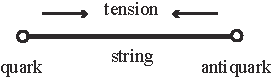
\includegraphics{Ch5_string_model.pdf}
\vskip2mm
\caption{The string model of a meson.
%�X�g�����O���g�������\���̃��f���D
}
\label{fig:string_model}
\end{figure}%
%%============

Because the string has the tension $\tension$, it would collapse to a point. In order the string not to collapse, one needs to oscillate the string. Or if the string rotates, the string becomes stable by balancing the tension and the centrifugal force. 
%The angular momentum of such a relativistic string is proportional to the energy squared of the string: 
%If one solves the equation of motion of a relativistic string, the angular momentum of the string is proportional to the energy squared of the string: 
%�X�g�����O�͒��͂������Ă��邽�߁C���̂܂܂ł͈�_�ɂ‚Ԃ�Ă��܂��D��_�ɂ‚Ԃ�Ȃ��悤�ɂ���ɂ́C�X�g�����O��U��������K�v������D���邢�́C�i�U��������Ƃ����̂Ǝ��͓������ƂȂ̂����j��]����Β��͂Ɖ��S�͂��‚荇���āC����ɑ��݂��邱�Ƃ��ł���D���Θ_�I�ȃX�g�����O�̉^���������������ƁC���̂悤�ȃX�g�����O�̊p�^���ʂ̓X�g�����O�̃G�l���M�[�̓��ɔ�Ⴗ��F
%���̊֌W��{\bf ���b�W�F�O��}\index{��‚���������@���b�W�F�O��}�iRegge trajectory�j�ƌ����D
% added
%Equation~\eqref{eq:regge} can be understood from the dimensional analysis. 
But the angular momentum $J$ (or the oscillation) of the string contributes to the energy $M$ of the string, so there is a relation between $J$ and $M$. 

Such a relation can be obtained from the dimensional analysis. We consider the relativistic string and use the unit $c=1$. In this unit, $[J] =\text{M}\text{L}$ and $[\tension] = \text{M}\text{L}^{-1}$. (Recall $\vec{J}=\vec{r}\times\vec{p}$. The mass density has the same dimensions as $\tension$ in these units.) Classically, such a string has only the tension $\tension$ as the dimensionful parameter [see, \eg, \eq{NG}]. Thus, we must have 
\be
%
J \simeq \frac{1}{\tension} M^2 + \hbar~.
\label{eq:pre_regge}
%
\ee
Here, we added the second term which is a quantum correction. 

% improved
Indeed, the meson spectrum satisfies such a relation. Phenomenologically, the relation \eqref{eq:pre_regge} is fitted by two parameters $\alpha'$ and $\alpha(0)$:
\be
%
J= \alpha' M^2+\alpha(0)~.
\label{eq:regge}
%
\ee
From the above discussion, $1/\alpha'$ represents the tension, and $\alpha(0)$ represents the quantum correction. (Note that in the units $c=\hbar=1$, $[\alpha'] =\text{L}^2$ and $\alpha(0)$ is dimensionless.) This relation is known as a \keyword{Regge trajectory}. Figure~\ref{fig:regge} is the Regge trajectory for typical mesons%
\footnote{Such a figure is known as a Chew-Frautschi plot \cite{Chew:1962eu}.}. 

The pions are the most well-known among all mesons. They are made of $u$ and $d$ quarks as well as their antiquarks. The $\rho$ mesons are also made of them. Although the pions have spin 0 (scalar meson), the $\rho$ mesons have spin 1 (vector meson) and heavier mass. Now, there is a series of mesons which are similar to the $\rho$ mesons but have larger spins and heavier masses. These mesons lie on a single line with%
\footnote{To be precise, this line does not represent a single trajectory but represents degenerate trajectories which are distinguished by the other quantum numbers. Incidentally, the $\omega$ mesons contain $s\bar{s}$, but they are similar to the $\rho$ mesons in the sense that they do not carry quantum numbers such as strangeness, charm, bottom, and top.} 
%���\���̃X�y�N�g���́C�������ɂ��̂悤�Ȋ֌W�𖞂������Ƃ��m���Ă���D\fig{regge}�́C��\�I�ȃ��\���ɑ΂��ă��b�W�F�O�Ղ�`�������̂ł���%\footnote{���̎�̐}�� Chew-Frautschi �v���b�g�ƌ��� \cite{Chew:1962eu}�D}�D�p�C�I���̓��\���̑�\�i�����C$u$, $d$ �̃N�H�[�N�E���N�H�[�N�΂���Ȃ�D$\rho$���\���������ł���D�������C�p�C�I�����X�s��0�i�X�J���[���\���j�ł���̂ɑ΂��C$\rho$���\���̓X�s��1�i�x�N�g�����\���j�ł���C���d���D����ɁC$\rho$���\���Ɠ����悤�Ȑ����������C���傫�ȃX�s���E���ʂ����ˆ�Q�̃��\��������D������1�‚̃��b�W�F�O�Տ�ɕ���%\footnote{���m�ɂ́C����͒P��̋O�Ղł͂Ȃ��C�ق��̗ʎq���̈Ⴂ�ɂ���ĕ�������4�‚́u�k�ނ����v�O�Ղ�����킵�Ă���D�Ȃ��C$\omega$���\����$s\bar{s}$���܂ނ��C�X�g�����W�l�X�C�`���[���C�{�g�����̗ʎq���������Ȃ��_�͓����ł���D}�C
\be
%
\alpha' \approx 0.9 \text{GeV}^{-2}~, \qquad \alpha(0) \approx 0.5~.
\label{eq:regge_trajectory_fit}
%
\ee
%�Ƃ���ƁC����烁�\���̃X�y�N�g���Ƃ悭��v����D

%%============
\begin{figure}[tb]
\centering
%\hspace{0.25in}
\scalebox{0.8}{ 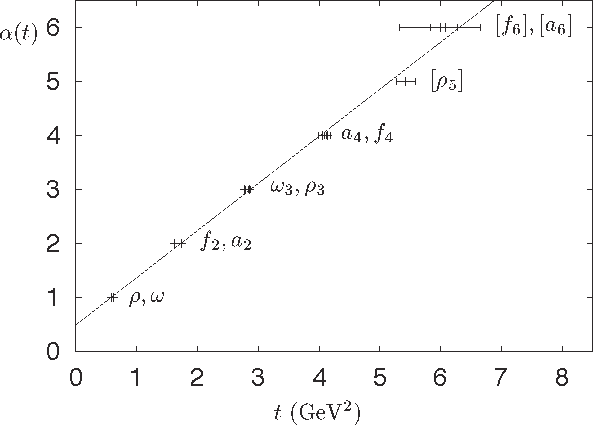
\includegraphics{Ch5_trajectory.pdf} }
\vskip2mm
\caption{An example of Regge trajectories. The horizontal axis represents $M^2$, and the vertical axis represents spins. The mesons in square brackets are not well-known. The straight line is fitted using \eq{regge_trajectory_fit}. Reproduced with permission from Ref.~\cite{Donnachie:2002en}.
% ���b�W�F�O�Ղ̗�D������$M^2$�C�c���̓X�s��������킷�D�p�J�b�R�̗��q�ɂ‚��ẮC���܂�悭�킩���Ă��Ȃ��D������\eq{regge_trajectory_fit}���g���ăt�B�b�g�������́D
}
\label{fig:regge}
\end{figure}%
%%============

%%============
\begin{figure}[tb]
\centering
%\hspace{0.25in}
\scalebox{0.5}{ 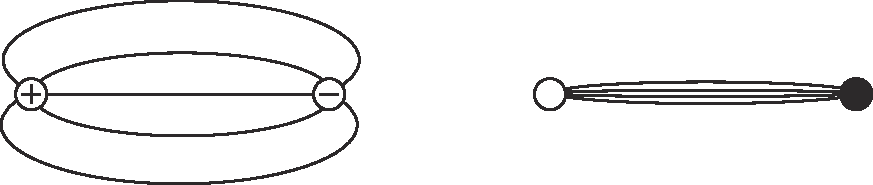
\includegraphics{Ch5_flux_tube.pdf} }
\vskip2mm
\caption{The QCD flux lines form a thin flux tube (right) unlike the electromagnetic flux lines (left).
%�d���C�w�̗͐��i���j�ƈႢ�CQCD�̗͐��̓t���b�N�X�`���[�u���Ȃ��i�E�j�D
}
\label{fig:flux_tube}
\end{figure}%
%%============

The mesons are explained by the string model well. Of course, eventually QCD appeared as the theory of strong interaction, but the string model is not inconsistent with QCD. The flux lines of electrodynamics spread in space. However, color flux lines do not spread but rather form a thin \keyword{flux tube} because gluons have self-interactions (\fig{flux_tube}). It is natural to imagine that mesons are well-described by the string model when the thickness of the flux tube is negligible. 
%�܂��CQCD���o�ꂵ���ƌ����Ă��CQCD�͋������ݍ�p�Ƃ��Ă̒������_�Ƒ�����Ȃ����̂ł͂Ȃ��D�ʏ�̗͐��͋�ԓI�ɍL�����Ă����i\fig{flux_tube}�j�D�������CQCD�̏ꍇ�C�O���[�I�������ȑ��ݍ�p�����‚��߁C�N�H�[�N�E���N�H�[�N�Ԃ̗͐��͊g���炸{\bf �t���b�N�X�E�`���[�u}\index{�ӂ�‚�������[��@�t���b�N�X�E�`���[�u}���Ȃ��ƍl�����Ă���D���Ȃ��Ƃ��C���̃t���b�N�X�E�`���[�u�̑����������ł���ꍇ�́C���\���̃X�g�����O�͌^�ɋA������ƍl����͎̂��R�ł���D

Thus, string theory has nice properties as a theory of strong interaction, but there are shortcomings as well. In particular, 
%���̂悤�ɁC�������ݍ�p�̕����ƒ������_�͂��܂��Ή����邪�C�����̖����������D�Ƃ���
\begin{description}

\item[Problem 1:] In order to quantize the string consistently, one needs a higher dimensional spacetime. The bosonic string, which contains only bosons in the spectrum, requires 26-dimensional spacetime, and string theory which also contains fermions requires 10-dimensional spacetime. Otherwise, the theory is not consistent. 
%�X�g�����O�𖵏��Ȃ��ʎq������ɂ́C���������󂪗v�������D�{�]�������̃X�g�����O�̏ꍇ��26��������C�t�F���~�I�����܂񂾒������_��10��������ł͂Ȃ��Ɩ������ł͂Ȃ��D
\item[Problem 2:] One can describe the confinement as a string connecting quarks, but what appears in QCD is not only the confining potential. When the quark separation becomes smaller, the thickness of the flux tube is no longer negligible, and the flux lines look more like the usual one. As a consequence, one has the Coulomb-like potential, $E \propto -1/\calR$. The simple string model is unlikely to describe this effect. Also, in the plasma phase, one has the Debye screening by thermally excited light quarks. From the string model point of view, the string becomes easier to break by quark pairs, but this implies that the string description is not very adequate. In a nutshell, the string model looks like a model of confinement only. If string theory really describes QCD, one should be able to discuss the full phase diagram of QCD.
%�N�H�[�N���‚Ȃ��X�g�����O�Ƃ��ĕ‚����߂͋L�q�ł������CQCD�ŏo�Ă���͕̂‚����߃|�e���V���������ł͂Ȃ��D�N�H�[�N�Ԃ̋������������Ȃ�΁C�t���b�N�X�E�`���[�u�̑����������ł��Ȃ��Ȃ�C�ʏ�̗͐��Ɏ��Ă���D���̌��ʂƂ��āC�|�e���V�����̓N�[�����^�ɂȂ�i$E \propto -1/\calR$�j�D�������C�P���ȃX�g�����O�͌^�ł́C���̌��ʂ͋L�q�ł������ɂȂ��D�܂��v���Y�}���ł́C�M�I�ɗ�N���ꂽ�N�H�[�N�E���N�H�[�N�΂ɂ���āC�X�g�����O��������₷���Ȃ��ăf�o�C�Օ����N����D�����ł���͂�C�X�g�����O�ɂ��L�q�͓K�؂ł͂Ȃ��Ȃ�悤�Ɏv����D�‚܂�C�X�g�����O�͌^�͕‚����߂̃��f���ɂ����Ȃ��悤�Ɏv����D�������_����������QCD������킷�̂Ȃ�C���}�̑S�̂��c�_�ł���ׂ��ł��낤�D
%���F�f�o�C�Օ��ɂ͂ق��̊�^�DAdS/CFT�ł̃f�o�C�Օ��ɋ߂��̂͂�����H

\end{description}
We will reexamine Problem~1 in \sect{reexamination} and Problem~2 in \sect{wilson_intuitive}. 
%���1�ɂ‚��Ă�\sect{reexamination}�C���2�ɂ‚��Ă�\sect{wilson_intuitive}�ōēx�������邱�Ƃɂ���D

These problems suggest that something is clearly missing about the correspondence between the strong interaction and string theory. Moreover, QCD was proposed, and QCD was proved to be the right theory of the strong interaction as experimental results accumulated. So, string theory as the strong interaction was once abandoned. Rather, string theory was reincarnated as the unified theory including gravity. We will then quickly look at this aspect of string.
%���̂悤�Ȗ�肩��C�������ݍ�p�ƌ����_�̑Ή��ɂ́C���炩�ɂȂɂ��������_���������D�܂��CQCD���񏥂���C�������ݍ�p�̐��������_���Ƃ����������ʂ��W�܂�C�������ݍ�p�̗��_�Ƃ��Ă̌����_�͂�������͕������ꂽ�D�ނ���C�����_�͏d�͂��܂߂����ꗝ�_�Ƃ��čďo�����邱�ƂɂȂ����D�����ŁC���ɓ��ꗝ�_�Ƃ��Ă̌����_���ȒP�ɂ݂Ă������Ƃɂ��悤�D


%%%%%%%%%%%%%%%%%%%%%%
\section{String theory as the unified theory}%\label{sec:}
%%%%%%%%%%%%%%%%%%%%%%

%%============
\begin{figure}[tb]
\begin{center}
\begin{tabular}{lll}
%
Matter	& ~~6 kinds of quarks	& \\
		& ~~6 kinds of leptons	& \\
Forces	& ~~gravity	& general relativity (classical theory) \\
		& $\left. \begin{array}{l}
\text{electromagnetic force} \\
\text{weak force} \\
\text{strong force}
		  \end{array} \right\}$
& gauge theories (quantum theories) \\
Higgs boson &&
%
\end{tabular}
\caption{The standard model of elementary particles.}
\label{fig:standard_model}
\end{center}
\end{figure}
%%============

Figure~\ref{fig:standard_model} shows the contents of the standard model. There are 6 quarks and 6 leptons as matters and 4 forces act on matters. In principle, all phenomena can be understood with these elements, but the standard model has many shortcomings as well. We will not describe these shortcomings, but in brief, the problem is that the standard model is a disjointed framework. 
%\fig{standard_model}�́C�f���q�̕W���͌^�̍\���v�f��`�������̂ł���D���������グ��f���q�́C�N�H�[�N�ƃ��v�g���ŁC�����̗��q�ɂ�4��ނ̗͂������Ă���D�����I�ɂ́C���ׂĂ̌��ۂ͂����̗v�f�ŗ����ł��邪�C�W���͌^�ɂ͂��܂��܂Ȍ��_������D�����̌��_�ɂ‚��āC�ڂ����͏q�ׂȂ����C���_���ꌾ�Ō����΁C�܂Ƃ܂肪�Ȃ��Ƃ������Ƃɐs����D

This is particularly clear in the force sector. Gravity is described by general relativity and this is a classical theory. On the other hand, the other 3 forces are described by gauge theories, and gauge theories can be quantized. So, theoretical foundations and concepts for these forces are completely different. Now, string theory is the theory which unifies all these elements. 
%���̓_�����Ȃ̂��C���ݍ�p�̕����ł���D�d�͈ȊO��3�‚̗͂̓Q�[�W���_�ɂ���ċL�q����C����͗ʎq�����”\�ł���D����C�d�͈͂�ʑ��Θ_�ɂ���ċL�q�����ÓT�_�ł���C��ʑ��Θ_�̗ʎq���ɂ͒N���������Ă��Ȃ��D���������āC�����̗͂́C���̗��_�I�Ȋ�b��T�O���傫���قȂ�D�������_�́C�����܂Ƃ܂肪�Ȃ��v�f���܂Ƃ߂����邱�Ƃ��ł���D

%%------------------
\subsection{String oscillations and elementary particles
%�X�g�����O�̐U���Ƒf���q
}%\label{sec:}
%%------------------

The fundamental object in string theory is the very small string (\fig{string}). There are two kinds of string: \keyword{open strings} with endpoints and \keyword{closed strings} with no endpoints. 
% improved
The string has only the tension $\tension$ as the dimensionful parameter. Since $[\tension] = \text{L}^{-2}$, we introduce a parameter $l_s$ with the dimension of length%
\footnote{The parameters $\tension$, $\alpha'$, and $l_s$ are related by
\be
%
\tension = \frac{1}{2\pi\alpha'} =  \frac{1}{2\pi l_s^2}~.
%\label{eq:}
%
\ee
}. 
The parameter $l_s$ is called the \keyword{string length} and represents the characteristic length scale of the string. The string length $l_s$ is the only fundamental length scale in string theory. The string length is about $10^{-34}$ m. But currently the length we can see experimentally is about $10^{-17}$ m. So, macroscopically the string is just a point particle. 
%The typical length of the string is denoted as $l_s$ and is called the {\bf string length}\index{string length}. The string length is related to the parameter $\alpha'$ in \sect{prehistory} by $\alpha'=l_s^2$. The string length $l_s$ (or the string tension) is the only fundamental length scale in string theory.
%�������_�ł̊�{�I�ȕ��̂́C�L�яk�݂��邫��߂ď����������̃X�g�����O�ł���i\fig{string}�j�D�X�g�����O�ɂ́C�[�_��������{\bf �J��}\index{��������@�J��}�ƁC�[�_�������Ȃ�{\bf �Œ�}\index{�ւ�����@�Œ�}�̓��ނ�����D�����̃X�g�����O�͂���߂ď������C$10^{-34}$ ���[�g�����x�ƍl�����Ă���D����ɑ΂��āC���ݎ����Łu����v���Ƃ��ł��钷���͂������� $10^{-17}$ ���[�g�����x�ɂ����Ȃ��D���̂��ߋ����I�ɂ̓X�g�����O�͑f���q�Ƃ݂Ȃ���D�X�g�����O�̓T�^�I�Ȓ�����{\bf �X�g�����O����}\index{���Ƃ�񂭂Ȃ���@�X�g�����O����}�ƌĂсC$l_s$ �ł���킷�D�������_�̊�b�I�ȃX�P�[���́C$l_s$ �����ł���i\sect{NG}�j�D

But no matter how small the string is, there is a big difference between strings and point particles; namely, a string can oscillate and a string can oscillate in various ways. This is the advantage of the string. There are many kinds of elementary particles in particle physics. String theory unifies all particles in nature as different oscillations of string. 
%As I will show you shortly, an open string represents a gauge theory. A closed string represents a graviton. 
%�������C�ǂ�Ȃɏ������Ă��C�X�g�����O�Ɨ��q�ɂ͌���I�ȈႢ������D����́u�X�g�����O�͐U���ł���v�Ƃ����_�ł���D�����Ă��̓_�������C�������_�̗��_�ł���D�f���q�_�ł͂��܂��܂ȑf���q���o�ꂷ��D�������_�ł́C�����̑f���q�͂��ׂăX�g�����O�œ���I�ɗ��������D�X�g�����O�͂��낢��Ȍ`�ŐU���ł��邪�C���܂��܂ȑf���q�̓X�g�����O�̂��܂��܂ȐU���Ƃ��ĉ��߂���D

%%============
\begin{figure}[tb]
\centering
%\hspace{0.25in}
\scalebox{0.5}{ 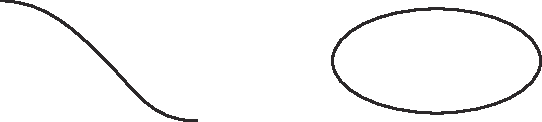
\includegraphics{Ch5_open_and_closed.pdf} }
\vskip2mm
\caption{Main ingredients of string theory. An open string with endpoints and a closed string without endpoints.}
%\caption{�������_�̎�ȓo��l���D�[�̂���X�g�����O�i�J���j�ƃ��[�v��̃X�g�����O�i�Œ��j�D}
\label{fig:string}
\end{figure}%
%%============

Let us look at string oscillations closely. 
%The easiest way to see that an open string represents a gauge theory is look at  how the string oscillates. 
Figure~\ref{fig:level1} shows the simplest open string oscillation (in four dimensions).
%\footnote{String theory is actually a 10-dimensional theory, but we discuss in 4-dimensions for illustrating purpose.} 
As one can see, the string can oscillate in two directions. So, the open string has two degrees of freedom at this level. These degrees of freedom represent two polarizations of a gauge field (photon). In this sense, the open string represents a gauge theory%
% added
\footnote{Classically, such a string oscillation represents a massive particle as one can expect from \eq{regge}. But it is actually massless because of the quantum correction [the second term of \eq{regge}]. This is true only in 26-dimensional spacetime for the bosonic string and in 10-dimensional spacetime for superstrings. This is one reason why higher-dimensional spacetime is necessary in string theory. }. 
%��̓I�ɃX�g�����O�̐U���̗l�q�����Ă݂悤�D�܂��J���̐U�����l����D\fig{level1} �́C�J���̈�ԒP���ȐU���������������̂ł���i4��������̏ꍇ�j�D�X�g�����O�͐U�����Ă��邪�C�U����������ɂ�2�‚���D����̓Q�[�W��i���q�j��2�‚̕Ό���Ԃ�����킷�D���̈Ӗ��ŁC�J���̓Q�[�W���_������킷�D

On the other hand, a closed string represents a graviton. Again, the easiest way to see this is to look at how the string oscillates (\fig{closed}). In general, the oscillations on a string have two modes: the left-moving mode and right-moving mode. For an open string, these modes mix each other at endpoints, but these modes become independent for a closed string. So, one can oscillate the right-moving mode in one direction and the left-moving mode in the other direction. In a sense, a closed string oscillates in two directions simultaneously. This property explains the spin-2 nature of the graviton. In fact, a graviton also oscillates in two directions simultaneously%
\footnote{More precisely, the simplest oscillations of a closed string represents a graviton and two undiscovered scalar particles, the dilaton\index{dilaton} and the axion. Since left and right-moving modes each have two degrees of freedom, a closed string has four degrees of freedom at this level (in four dimensions). The graviton has only two degrees of freedom, and two scalar fields cover the remaining degrees of freedom.}.
%�ł́C�Œ��͂ǂ�ȗ��q������킵�Ă���̂��낤�H�@�i�s�g�̐i�ޕ����ɂ́C���v���Ɣ����v����2�ʂ肪����i\fig{closed}�j�D�[������ꍇ�C�[�ł���2�‚͍����肠���Ă��܂��D�������C�Œ��ł͒[���Ȃ��̂ŁC����2�‚͓Ɨ��ł���D���̂��߁C���Ƃ��Ύ��v���̔g���㉺�����ɐU�������āC�����v���̔g�͂���Ƃ͈Ⴄ�����ɐU�������邱�Ƃ��ł���D�‚܂�C�Œ��́C������2�‚̕����ɐU���ł���D

%����́C���傤�Ǐd�͏�i�O���r�g���j�̐����ƈ�v����D�d�͏�́u�Ό��v�ɂ‚��ẮC���Ȃ��݂�������������Ȃ����C�d�͏��������2�‚̕����ɐU�����Ă���C���̐������X�s��2�ƌ���%
%\footnote{
%�������́C�Œ��̂����Ƃ��P���ȐU���́C�O���r�g���ƁC�������̃X�J���[���q�C�f�B���g��\index{�Ă���Ƃ�@�f�B���g��}�ƃA�N�V�I��������킷�D���̏ꍇ�C�U���̉”\����2�ʂ肾�����D���܂̏ꍇ�́C���ꂼ��̐i�s�g��2�ʂ�̕����ɐU���ł���D���������āC���v�����4�ʂ�̐U��������D�O���r�g���̎��R�x��2�‚Ȃ̂ŁC2�‚̃X�J���[���q�Ƃ��킹�C���q�̕`���ł����v����4�‚̎��R�x�����邱�ƂɂȂ�D}�D

%%============
\begin{figure}[tb]
\centering
%\hspace{0.25in}
\scalebox{0.5}{ 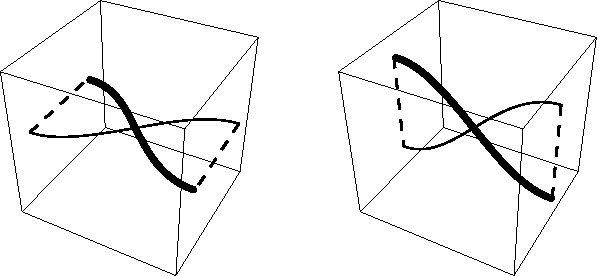
\includegraphics{Ch5_open_level1_v2_75.pdf} }
\vskip2mm
\caption{The simplest oscillations of an open string. The initial configurations in thick curves become gray curves after the half period. The ``box" here is drawn to see the oscillations easier.}
%�J���̂����Ƃ��P���ȐU���D�����̊J������������ɃO���[�̐��̌`���Ƃ�D�u���v�͒P�ɂR�����ł̐U�������₷�����邽�߂ɕ`�������̂ł���D
\label{fig:level1}
\end{figure}%
%%============

%%============
\begin{figure}[!tb]
\centering
%\hspace{0.25in}
\scalebox{0.75}{ 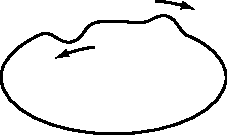
\includegraphics{Ch5_closed.pdf} }
\vskip2mm
\caption{A closed string has two independent modes, which corresponds to the spin-2 nature of the graviton.}
%�Œ��ł́C2�‚̓Ɨ��Ȑi�s�g������D����̓O���r�g���̂��ƒX�s��2�̐����ƈ�v����D
\label{fig:closed}
\end{figure}%
%%============

%%------------------
\subsection{D-brane}\label{sec:D_brane_primer}
%%------------------

An open string propagates through spacetime just like a closed string, but an open string can also have its endpoints on an object, the so-called \keyword{D-brane} [\fig{Dbrane}] \cite{Dai:1989ua,Polchinski:1995mt}. 
% w/ D-brane primer version
%The open string I consider below is always of this type. 
Although these open strings are constrained to have their endpoints on the D-brane, these are open strings, so they still describe gauge theories. But because the endpoints are constrained on the D-brane, the gauge theory described by the D-brane is localized on the D-brane. 
%�������_�ɂ�{\bf D�u���[��}\index{D�ӂ�[��@D�u���[��}�ƌĂ΂�镨�̂����݂��� [ \fig{Dbrane} ]�D�J���͂���D�u���[����ɒ[�_�����‚��Ƃ��ł���D�ȉ��ōl����J���͂��‚����̃^�C�v�ł���D�[�_���Œ肳��Ă��Ă�����͊J���Ȃ̂ŁC��͂�Q�[�W���_������킷�D�����C�J����D�u���[����ɒ[�_�������Ă���̂ŁC���̃Q�[�W���_��D�u���[����ɋǍ݂��Ă���D

If there are $N_c$ coincident D-branes, open strings can have endpoints in various ways. Open strings can have endpoints on the same brane or can have endpoints on the different branes [two curved lines and one straight line in \fig{Dbrane_SYM}].
%[two solid lines and one dotted line in \fig{Dbrane_SYM}]. 
These new degrees of freedom correspond to $SU(N_c)$ degrees of freedom%
\footnote{More precisely, the D-branes represent a $U(N_c)$ gauge theory, but the $U(1)$ part describes the center of mass motion of the branes and decouple from the $SU(N_c)$ part.}.
%D�u���[���́C�������d�Ȃ肠�����Ƃ��ł���D����ƁC�J����D�u���[����ɒ[�_�����‚��C�[�_��ʁX��D�u���[����ɒu�����Ƃ��ł��� [ \fig{Dbrane_SYM} �ŁC�����̂��̓��ނƓ_���̂��� ]�D���̂��炽�Ȏ��R�x�́C���̏ꍇ�̃Q�[�W���_��$U(1)$ �Q�[�W���_�ł͂Ȃ��C$SU(N_c)$ �Q�[�W���_������킷���Ƃ��Ӗ�����i$N_c$ �̓u���[���̖����j%
%\footnote{���m�ɂ�$U(N_c)$�Q�[�W���_������킷���C$U(1)$�����̓u���[���̏d�S�^���ɑ������C$SU(N_c)$������decouple����D}�D

The D-branes arise with various dimensionalities. A D-brane with a $p$-dimensional spatial extension is called the D$p$-brane\index{Dp-brane@D$p$-brane}. Namely, 
%���܂��܂Ȏ�����D�u���[�������݂���D$p$�����̋�ԓI�L�����������D�u���[���̂��Ƃ�D$p$�u���[���ƌĂԁD�‚܂�C
\begin{center}
\begin{tabular}{cc}
%
$ p=0 $		& point-like object \\
$ p=1 $		& string-like object \\
$ p=2 $		&\hspace{5mm} membrane-like object \\
$ \vdots $	& $ \vdots $
%
\end{tabular}
\end{center}
Thus, the D$p$-brane describes a $(p+1)$-dimensional gauge theory. We are interested in four-dimensional gauge theories, so consider the D3-brane in order to mimic QCD%
\footnote{This is not necessarily the case if one compactifies part of brane directions (\eg, Sakai-Sugimoto model \cite{Sakai:2004cn}). Incidentally, the D1-brane is a string-like object, but it is different from the ``fundamental string" we have discussed so far. 
}.
%���������āCD$p$�u���[����$(p+1)$�����̃Q�[�W���_������킷�D��X��4��������ł̃Q�[�W���_�ɋ���������̂ŁCQCD�Ɏ������_���l����ɂ�D3�u���[�����l����΂悢���ƂɂȂ�%
%\footnote{�u���[���̈ꕔ�̕������u�ۂ߂�v�̂ł���΁C�K������D3�u���[���Ɍ�����킯�ł͂Ȃ��i���Ƃ��Ύ���-���{�͌^\cite{Sakai:2004cn}�j�D�Ȃ��CD1�u���[���̓X�g�����O�I�ȕ��̂����C����܂ŋc�_���Ă����X�g�����O�i��{���j�Ƃ͈Ⴄ���̂ł���D
%}�D

The D-branes are related to the black branes in \sect{black_branes}. Some of black branes are gravitational descriptions of D-branes.

% w/ D-brane primer version
In \sect{D3_brane}, we discuss more about the D-brane, the gauge theory that the D3-brane represents, and its role in AdS/CFT.

%%============
\begin{figure}[tb]
\centering
\subfigure[]{
\scalebox{0.75}{ 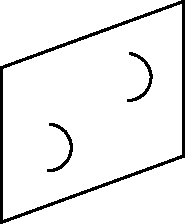
\includegraphics{Ch5_Dbrane.pdf} }
\label{fig:Dbrane} } \qquad
\subfigure[]{
\scalebox{0.75}{ 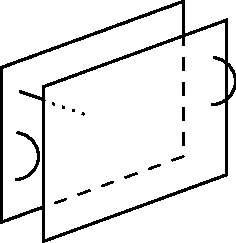
\includegraphics{Ch5_SYM.pdf} }
\label{fig:Dbrane_SYM} }
\vskip2mm
\caption{
(a) An open string can have endpoints on a D-brane. (b) The $N_c$ coincident D-branes represent a $SU(N_c)$ gauge theory. In the figure, the branes are separated for illustration, but we consider the coincident branes in reality.
%�J���́CD�u���[���ƌĂ΂�镨�̏�ɒ[�_�����‚��Ƃ��ł���D(b) D�u���[���� $N_c$ ������ƁC$SU(N_c)$ �Q�[�W���_�ɂȂ�D�}������s����C�u���[���𗣂��ĕ`���Ă��邪�C���ۂɂ͏d�Ȃ������̂��l����D
}
\label{fig:Dbranes}
\end{figure}%
%%============


%%------------------
\subsection{Why open and closed strings?}%\label{sec:}
%%------------------

In string theory, there are two kinds of strings, the open string and the closed string. Why are there two kinds of strings? Or one would say that string theory is not a unified theory since there are two kinds of strings. But actually these are the same object in a sense. To see this, let us consider how strings interact with each other.  
%�������_�ł́C��ʂɊJ���ƕŒ��C2��ނ̃X�g�����O������D�Ȃ�2��ނ���̂��낤�H�@���邢�́C�������_��2��ނ̃X�g�����O������̂œ��ꂳ��Ă��Ȃ��ł͂Ȃ����C�Ǝv���邩������Ȃ��D�������C���ۂɂ͂����͂���Ӗ��������̂ł���D������݂邽�߂ɂ́C�X�g�����O�̑��ݍ�p���l����K�v������D

\fig{open_vs_closed1} is the simplest interaction for open strings. Two open strings join into one open string. But if the endpoints of two open strings can join, the endpoints of a single open string can join as well. Otherwise, one has to require a nonlocal constraint on the string dynamics. Thus, the endpoints of a single open string can join to produce a closed string. Namely, if there are open strings, one has to have closed strings. This is the reason why we have two kinds of strings%
\footnote{One can consider string theories with closed string alone, but we will not discuss such theories.}. 
%�͊J���̂����Ƃ��ȒP�ȑ��ݍ�p�ł���D2�‚̊J����1�‚ɂ����‚��D�������C2�‚̊J���̒[�_�������‚��̂ł���΁C1�‚̊J���̒[�_�ǂ����������‚��͂��ł���D�����łȂ���΁C�X�g�����O�̃_�C�i�~�N�X�ɔ�Ǐ��I�ȍS����u�����ƂɂȂ��Ă��܂��D���������āC1�‚̊J���̒[�_�͂����‚����Ƃ��ł��āC�Œ������o���͂��ł���D�‚܂�C�J��������ƁC�Œ����Ȃ���΂����Ȃ��D2��ނ̃X�g�����O������̂͂��̂��߂ł���%
%\footnote{�Œ������̒������_���l���邱�Ƃ��ł��邪�C�{���ł͋c�_���Ȃ��D}�D

Because an open string represents a gauge theory and a closed string represents gravity, string theory must contain both gauge theory and gravity. This is the unique feature of string theory as the unified theory.
%�J���̓Q�[�W���_�C�Œ��͏d�͂�����킷�̂�����C�������_�̓Q�[�W���_���d�͗��_���܂܂Ȃ���΂����Ȃ����ƂɂȂ�D����́C���ꗝ�_�Ƃ��Ă̒������_�̃��j�[�N�ȓ_�ł���D

The AdS/CFT duality utilizes this unique feature. The AdS/CFT duality relates a gauge theory to a gravitational theory. This is possible only for the unified theory such as string theory. In conventional field theory, a gauge theory and a gravitational theory are completely separated since theoretical foundations and concepts are very different. As a result, there is no way to get a relation between a gauge theory and a gravitational theory. 
%���̓��ꗝ�_�Ƃ��Ă̒������_�̗��_�������ɏo�Ă���Ⴊ�CAdS/CFT�ł���DAdS/CFT�́C�Q�[�W���_�Əd�͗��_���������Ǝ咣����D����̓Q�[�W���_�Əd�͗��_�𓝈ꂷ�钴�����_�����炱���C�”\�ɂȂ����l���ł���D�ʏ�̏�̗��_�ł́C����2�‚͗��_�I�Ȋ�b��T�O���傫���قȂ�̂ŁC���̂悤�Ȋ֌W�͖]�ނׂ����Ȃ��D

There is a bigger picture behind AdS/CFT. Namely, AdS/CFT requires the existence of a unified theory behind. 
%AdS/CFT�̔w��ɂ́C``big picture" ������D���Ȃ킿�CAdS/CFT �͔w��ɓ��ꗝ�_�̑��݂�v�����Ă���̂ł���D

%%============
\begin{figure}[tb]
\centering
%\hspace{0.25in}
\scalebox{0.75}{ 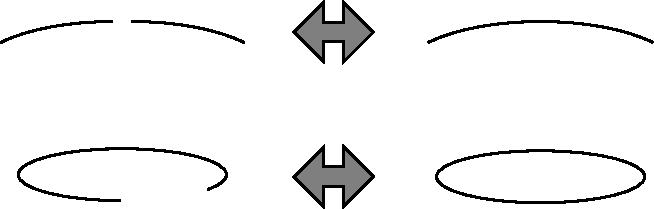
\includegraphics{Ch5_open_vs_closed1.pdf} }
\vskip2mm
\caption{\textit{Top}: the simplest interaction for open strings is the joining of two strings into one. \textit{Bottom}: if the endpoints of two open strings can join, the endpoints of a single open string can join as well.}
%�J���̂����Ƃ��ȒP�ȑ��ݍ�p�́C�J����1�‚ɂ����‚����Ƃł���i��̐}�j�D�����ł���΁C1�‚̊J���̒[�_�ǂ����������‚��ĕŒ��ɂȂ�͂��ł���i���̐}�j�D}
\label{fig:open_vs_closed1}
\end{figure}%
%%============


%%------------------
\subsection{String interactions
%���̑��ݍ�p
}\label{sec:string_interaction}
%%------------------

%%============
\begin{figure}[tb]
\centering
\subfigure[]{
\scalebox{0.75}{ 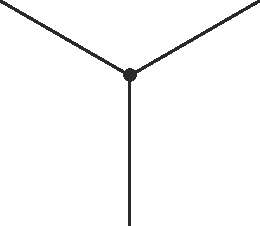
\includegraphics{Ch5_particle_vertex.pdf} }
} \qquad
\subfigure[]{
\scalebox{0.75}{ 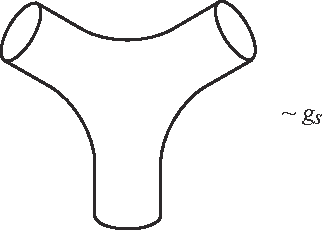
\includegraphics{Ch5_closed_vertex.pdf} }
}
\vskip2mm
\caption{
(a) A Feynman diagram which represents an interaction vertex. (b) The corresponding interaction for closed strings.}
%(a) ���ݍ�p������킷�t�@�C���}���E�_�C�A�O�����̒��_�D(b) �Ή�����Œ��̑��ݍ�p�D}
\label{fig:closed_vertex}
\end{figure}%
%%============

%%============
\begin{figure}[tb]
\centering
\scalebox{0.75}{ 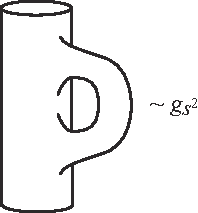
\includegraphics{Ch5_closed_loop.pdf} }
%\vskip2mm
\caption{A 1-loop of closed strings.}
%�Œ���1���[�v�D}
\label{fig:closed_loop}
\end{figure}%
%%============

%%============
\begin{figure}[tb]
\centering
%\hspace{0.25in}
\scalebox{0.75}{ 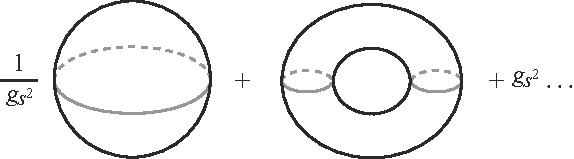
\includegraphics{Ch5_string_amplitude.pdf} }
\vskip2mm
\caption{The perturbative expansion of string theory is given by the sum over the topologies of world-sheet surfaces.}
%�����_�̐ۓ��W�J�́C�g�|���W�[�̑��������Ƃ��Ă���킳���D}
\label{fig:string_amplitude}
\end{figure}%
%%============

A particle draws a wold-line in spacetime. Similarly, a string sweeps a two-dimensional surface, a \keyword{world-sheet}, in spacetime. In \fig{closed_vertex}(a), we draw a Feynman diagram for a particle, which represents an interaction vertex. For a closed string, such an interaction is replaced by \fig{closed_vertex}(b).
%���q�͎��󒆂Ő��E����|���D���l�ɁC�X�g�����O��2�����ʁC{\bf ���E��}\index{�������߂�@���E��}�iworld-sheet�j��|���D\fig{closed_vertex}(a) �́C���q�̑��ݍ�p������킷�t�@�C���}���E�_�C�A�O�����̒��_��`�������̂ł���D���̂悤�ȑ��ݍ�p�́C�Œ��̏ꍇ\fig{closed_vertex}(b) �̂悤�ɂȂ�D

In order to express the strength of the interaction, we assign the \keyword{string coupling constant} $g_s$ for an emission/absorption of a closed string. A closed string 1-loop (\fig{closed_loop}) has an emission and an absorption of a virtual closed string, so it is proportional to $g_s^2$. Figure~\ref{fig:closed_loop} has one ``handle," so we can rephrase the rule to assign $g_s^2$ for each handle. If we have one more loop, we have one more handle, so the diagram has the factor $g_s^4$.
%���̑��ݍ�p�̋���������킷�̂ɁC�Œ��̕��o�E�z���̃v���Z�X��{\bf �X�g�����O�����萔}\index{���Ƃ�񂭂��‚����Ă�����@�X�g�����O�����萔}$g_s$ �̈��q��t�^���邱�Ƃɂ���D���q��1���[�v�ɑ�������̂�\fig{closed_loop} �ł���C����� $g_s^2$ �ɔ�Ⴗ��D\fig{closed_loop} �́u�n���h���v��1�‚���̂ŁC�n���h��1�‚����� $g_s^2$ �����肠�Ă�ƌ����Ă��悢�D���[�v�̐�������1�‘�����ƁC�n���h���������1�‘����C$g_s^4$ �ƂȂ�%
%\footnote{���΂��΁C�ȒP�̂��߂ɐ^��_�C�A�O�����������o�ꂷ�邪�C�K���ȊO���������ĎU���U���ƍl���Ă������D�Ȃ��C���̒i�K�ł� $g_s$ �͗��_�̃p�����[�^�̂悤�ɂ݂��邪�C���͂����ł͂Ȃ��i\sect{SUGRA}�j�D}�D

To summarize, string interactions are classified by the world-sheet topologies (\fig{string_amplitude})%
\footnote{Below we often consider only vacuum amplitudes for simplicity, but one can consider scattering amplitudes by adding appropriate external lines. Incidentally, $g_s$ looks like a free parameter of the theory at this stage, but actually it is not a free parameter (\sect{SUGRA}).}. 
If we denote the number of handles (genus) as $h$, a $h$-loop has the factor $g_s^{2h}$. The genus $h$ is related to the Euler characteristic $\chi$ by $\chi=2-2h$, and vacuum amplitudes can be written as $1/g_s^\chi$ using the Euler characteristic%
\footnote{If one adds three external lines (factor $g_s^3$) to the sphere $1/g_s^2$, the diagram is proportional to $g_s$, which is consistent with the interaction vertex in \fig{closed_vertex}(b).}. 
%���ǁC�X�g�����O�̑��ݍ�p�̓g�|���W�[�ŕ��ނł��邱�ƂɂȂ�i\fig{string_amplitude}�j�D�n���h���̐��i�W�[�i�X�j$h$���g���ƁC$h$���[�v�� $g_s^{2h}$ �ƂȂ�D�W�[�i�X�̓I�C���[�W�� $\chi$ �� $\chi=2-2h$ �̊֌W������̂ŁC�^��_�C�A�O�������I�C���[���� $1/g_s^\chi$ �Ə������Ƃ��ł���%
%\footnote{�� $1/g_s^2$ �ɕŒ��̊O����3�‰�����Ɓi$g_s^3$�j�C ��������\fig{closed_vertex}(b) �̑��ݍ�p $g_s$ �ɔ�Ⴗ��D}�D

The open string case is similar. Assign the open string coupling constant $\tilgs$ for an emission of an open string. Then, the open string interactions are classified by the topologies of world-sheets with holes (\fig{open_vertex}). However, the open string naturally accompanies the closed string as we saw earlier,  and open string interactions are related to closed string interactions. In fact, an open string 1-loop can be viewed as an emission of a closed string (\fig{open_vs_closed2}), so we obtain 
%�J���ɂ‚��Ă����l�ł���D�J���̕���ɑ΂�$\tilgs$ �̈��q��t�^����ƁC�J����2�����ʂ̃g�|���W�[�ŕ��ނł���i\fig{open_vertex}�j�D�������C�J���ƕŒ������l����ꍇ�C����2�‚̑��ݍ�p�ɂ͊֌W�����邱�Ƃ�O���ɒu���K�v������D���ہC�J����1���[�v�́C�ό`����ƕŒ�1�‚̕��o�Ƃ݂Ȃ��邩��i\fig{open_vs_closed2}�j�C
\be
%
g_s \simeq \tilgs^2~.
%\label{eq:}
%
\ee
%�̊֌W�����肽�D

%%============
\begin{figure}[tb]
\centering
\subfigure[]{
\scalebox{0.75}{ 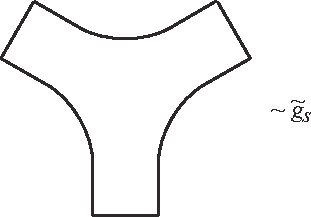
\includegraphics{Ch5_open_vertex.pdf} }
} \qquad
\subfigure[]{
\scalebox{0.75}{ 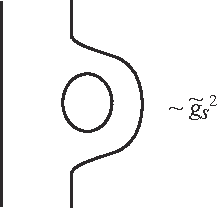
\includegraphics{Ch5_open_loop.pdf} }
}
\vskip2mm
\caption{(a) An open string interaction. (b) A 1-loop of open strings. }
%�J���̑��ݍ�p
%�J����1���[�v
\label{fig:open_vertex}
\end{figure}%
%%============

%%============
%\begin{figure}[tb]
%\centering
%\subfigure[An open string interaction.]{
%\scalebox{0.75}{ 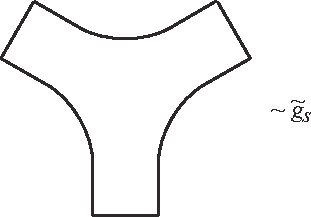
\includegraphics{Ch5_open_vertex.pdf} }
%} \qquad
%\subfigure[A 1-loop of open strings.]{
%\scalebox{0.75}{ 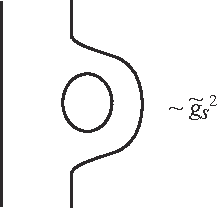
\includegraphics{Ch5_open_loop.pdf} }
%}
%\vskip2mm
%\caption{}
%\label{fig:open_vertex}
%\end{figure}%
%%============

%%============
\begin{figure}[tb]
\centering
\scalebox{0.75}{ 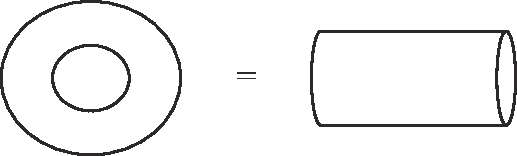
\includegraphics{Ch5_open_vs_closed2.pdf} }
\vskip2mm
\caption{An open string 1-loop can be viewed as an emission of a closed string.}
%�J����1���[�v�́C�ό`����ƕŒ�1�‚̕��o�Ƃ݂Ȃ���D}
\label{fig:open_vs_closed2}
\end{figure}%
%%============

%\afterpage{\clearpage}

%%------------------
\subsection{Supergravity: classical gravity approximation of string theory
%�������_�̌ÓT�d�͋ߎ��F���d�͗��_
}\label{sec:SUGRA}
%%------------------

We have seen that the simplest oscillations of strings correspond to gauge theories and gravity. But a string has an infinite number of harmonics, so string theory predicts an infinite number of elementary particles. Since string oscillations cost energy, these infinite number of harmonics correspond to massive particles whose masses are determined by energy of oscillations. This mass is typically $O(1/l_s)$, which is extremely heavy as elementary particles. Thus, what normally matters is a set of the lowest oscillations only; they correspond to known particles.
%�X�g�����O�̂����Ƃ��P���ȐU������C�Q�[�W���O���r�g�����o�Ă��邱�Ƃ��݂����C���̌ŗL�U���͖����ɂ���̂ŁC�������_�͖����‚̑f���q�̑��݂�\�����邱�ƂɂȂ�D�����Ƃ��C�X�g�����O���U������ƁC�U���̓G�l���M�[�����‚̂ŁC�����I�ɂ͐U���̃G�l���M�[���̎��ʂ����‘f���q�Ƃ��Ă݂���D���̎��ʂ́C�T�^�I�ɂ�$O(1/l_s)$�Ƃ����f���q�Ƃ��Ă͂����ւ�d�����ʂ����D���̂��߁C�ʏ�����Ƃ��Ⴂ�U���݂̂��d�v�ɂȂ�D����炪�ʏ�m���Ă���f���q�ł���D

String theory describes a finite number of known particles when one can ignore the string length $l_s$, so string theory should be written by standard field theories. Moreover, when $g_s \ll 1$, only the lowest order of topology expansion, tree diagrams, dominates. In such a case, classical field theories should be enough to describe string theory. Such a theory is known as \keyword{supergravity}%
\footnote{See Ref.~\cite{Freedman:2012zz} for a textbook of supergravity. The name, supergravity, comes from the fact that the theory has local supersymmetry, but we will not discuss the terms with fermions below.}.
%���̂悤�Ɍ��̍L���� $l_s$ ���\���ɏ������Ƃ݂Ȃ���Ƃ��́C�������_�͏����̒m���Ă���f���q�ł���킳���̂ŁC�ӂ‚��̏�̗��_�ŏ�����͂��ł���D����ɁC$g_s \ll 1$ �Ńg�|���W�[�W�J�̍Œ᎟�C�c���[�E�_�C�A�O�����������x�z�I�ȏꍇ�́C��̌ÓT�_�ŏ\���Ȃ͂��ł���D���ہC���̂悤�ȗ��_��{\bf ���d�͗��_}\index{���悤���䂤��悭����@���d�͗��_}�isupergravity�j�Ƃ��Ēm���Ă���%
%\footnote{�Ǐ��I���Ώ̐������d�͗��_�Ȃ̂ł��̖��O���‚��Ă��邪�C�ȉ��ł̓t�F���~�I�����܂ލ��ɂ‚��Ă͋c�_���Ȃ��D}�D

The form of supergravity action can be determined from general principles%
\footnote{More properly, one calculates string Feynman diagrams as in \sect{string_interaction} and writes down a field theory action which reproduces these scattering amplitudes.}.
For example, one can show that string theory graviton has general covariance, so the gravity part should be given by
%���d�͗��_�̌`�́C������x��ʓI�ȍl�@���猈�߂邱�Ƃ��ł���%
%\footnote{�����ɂ́C\sect{string_interaction}�̂悤�ɃX�g�����O�̃t�@�C���}���E�_�C�A�O�������v�Z���āC���̂悤�ȎU���U����^�����̗��_�̍�p���\�����邱�Ƃœ�����D}�D
%���Ƃ��΁C�������_�̃O���r�g������ʍ��W�ϊ��s�ϐ������‚��Ƃ��������Ƃ��ł���̂ŁC�d�͕����͈�ʑ��Θ_�Ɠ��l��
\be
%
\action = \frac{1}{16\pi G_{10}} \int d^{10}x\, \sqrt{-g} R
\label{eq:sugra_leading}
%
\ee
just like general relativity. We write it as a 10-dimensional action since superstring theory can be quantized consistently only in 10-dimensional spacetime. $G_{10}$ is the Newton's constant in 10-dimensional spacetime. Similarly, one can show that gauge fields in string theory have gauge invariance, so the gauge theory part should be given by the usual gauge theory action.
%�Ƃ����`�ŗ^������͂��ł���D�������C�������_��10��������ł͂Ȃ��Ɩ����Ȃ��ʎq���ł��Ȃ��̂ŁC10�����̍�p�Ƃ��ď������D$G_{10}$ ��10�����̃j���[�g���萔�ł���D���l�ɁC�Q�[�W��ɑ΂��Ă��Q�[�W�s�ϐ������‚��Ƃ��������Ƃ��ł���̂ŁC�ʏ�̃Q�[�W��̍�p�ŗ^������͂��ł���D

In string theory, the fundamental coupling constant is the string coupling constant $g_s$. In supergravity, coupling constants are $G_{10}$ and the gauge field coupling constant $g_\text{YM}$. Then, one can relate $g_s$ to supergravity coupling constants. By expanding $g_{\mu\nu} = \eta_{\mu\nu} + h_{\mu\nu}$, the graviton action is schematically written as
%�������_�̊�{�I�Ȍ����萔��$g_s$�ł���D����C���d�͗��_�̌����萔�� $G_{10}$ ��Q�[�W��̌����萔 $g_\text{YM}$ �Ȃ̂ŁC$g_s$ �ƒ��d�͗��_�̌����萔�Ɋ֌W���‚��邱�Ƃ��ł���D$g_{\mu\nu} = \eta_{\mu\nu} + h_{\mu\nu}$�Ƃ���ƁC�O���r�g���̍�p�͌`���I��
\be
%
\action = \frac{1}{16\pi G_{10}}  \int d^{10}x\,  \{ \del h \del h + h \del h\del h + h^2 \del h\del h + \cdots \}~.
\label{eq:action_graviton}
%
\ee
This implies that a graviton emission is proportional to $G_{10}^{1/2}$. Since a closed string emission is proportional to $g_s$, one gets $G_{10} \propto g_s^2$.
%�ƂȂ�D������O���r�g���̕��o�� $G_{10}^{1/2}$ �ɔ�Ⴗ��D�Œ��̕��o�� $g_s$ �ɔ�Ⴕ���̂ŁC $G_{10} \propto g_s^2$ �ƂȂ�D

Similarly, the gauge field action is schematically written as%
\footnote{
% w/ D-brane primer version
We write the $(p+1)$-dimensional action instead of a 10-dimensional action because one can consider $(p+1)$-dimensional gauge theories using D-branes.
%Readers may wonder why I wrote the $(p+1)$-dimensional action instead of a 10-dimensional action. As we will see later, one can consider $(p+1)$-dimensional gauge theories even in string theory.
}
%�܂��Q�[�W��̍�p�́C�`���I��
\be
%
\action =  \frac{1}{g_\text{YM}^2} \int d^{p+1}x\, \{ \del A \del A+ A^2 \del A + A^4 \}~.
\label{eq:action_gauge}
%
\ee
This implies that a gauge field emission is proportional to $g_\text{YM}$. Since an open string emission is proportional to $\tilgs \simeq g_s^{1/2}$, 
%�ƂȂ�%
%\footnote{�����Ŏ��󎟌���10�����ł͂Ȃ��C$(p+1)$�����ɂƂ������Ƃ����Ԃ������v����������Ȃ����C���Ƃł݂�悤�ɒ������_�ł����Ă�$(p+1)$�����̃Q�[�W���_���l���邱�Ƃ��ł��邩��ł���D}�D
%������Q�[�W��̕��o�� $g_\text{YM}$ �ɔ�Ⴗ�邱�Ƃ��킩��D�J���̕��o�� $\tilgs \simeq g_s^{1/2}$ �ɔ�Ⴕ���̂ŁC 
\be
%
g_\text{YM}^2 \propto g_s~.
%\label{eq:}
%
\ee
%�ł���D

The dimensional analysis further constrains the form of field theory coupling constants. Since we usually take the metric as dimensionless, the Newton's constant has dimensions $[G_{10}] = \text{L}^{8}$ from \eq{action_graviton}. In string theory, the fundamental string scale is only the string length $l_s$ which represents the characteristic length scale of the string. Thus, $G_{10} \simeq g_s^2 l_s^8$. 
%So, one would define the 10-dimensional Planck length $l_{10}$ as $G_{10} \simeq l_{10}^8$. But in string theory, the fundamental string scale is only the string length $l_s$ which represents the characteristic length scale of the string. Thus, $G_{10} \simeq l_{10}^8 \simeq g_s^2 l_s^8$. 
Similarly, the gauge field has dimensions $[A] =\text{L}^{-1}$ from \eq{action_gauge}. In order for the action to be dimensionless, $[g_\text{YM}^2] = \text{L}^{p-3}$. Thus, $g_\text{YM}^2 \simeq g_s l_s^{p-3}$. To summarize, 
%�����萔�̎��������킹�Ă������D�v�ʂ͒ʏ햳�����ɂƂ�̂ŁC\eq{action_graviton}���j���[�g���萔�̎����� $[G_{10}] = \text{L}^{8}$ �ł���D����C�������_�̊�b�I�ȃX�P�[���́C�X�g�����O�̓T�^�I�Ȓ���������킷�u�X�g�����O�����v $l_s$ �����ł���i\sect{NG}�j�D���������āC���������킹��� $G_{10} \simeq g_s^2 l_s^8$ �ƂȂ�D���l�ɁC�Q�[�W��̎�����\eq{action_gauge}��� $[A] =\text{L}^{-1}$ �ł���D��p���������ł��邽�߂ɂ� $[g_\text{YM}^2] = \text{L}^{p-3}$ �ł���D���������āC���������킹��� $g_\text{YM}^2 \propto g_s l_s^{p-3}$ �ƂȂ�D�܂Ƃ߂�ƁC
\be
%
\boxeq{
G_{10} \simeq g_s^2 l_s^8~, \quad
g_\text{YM}^2 \simeq g_s l_s^{p-3}~.
}
\label{eq:string_vs_qft}
%
\ee

The action \eqref{eq:sugra_leading} is the approximation when one can ignore the string length $l_s$. When the string length can no longer be ignored, the action has an infinite number of terms with powers of curvature tensors such as
%\eq{sugra_leading} �Ȃǂ̓X�g�����O���� $l_s$ �������ł���Ƃ��̋ߎ������C�X�g�����O�����������ł��Ȃ��Ȃ��
\be
%
\action = \frac{1}{16\pi G_{10}} \int d^{10}x \sqrt{-g}\, (R + l_s^2 R^2 + \cdots)~.
\label{eq:sugra_alpha'}
%
\ee
Such corrections are known as \textit{$\alpha'$-corrections}\index{alpha'-corrections@$\alpha'$-corrections}%
\footnote{Recall that the parameter $\alpha'$ is related to the string length $l_s$ by $\alpha'=l_s^2$.}.
From the field theory point of view, these terms correspond to higher derivative terms in an effective field theory%
\footnote{See Ref.~\cite{Polchinski:1992ed} for a review of effective field theories.}, 
and they originated from integrating out massive fields with mass $O(1/l_s)$. Roughly speaking, these terms can be ignored when $l_s^2 R \ll 1$, or the length scale of the curvature is much larger than the string length. 
%�̂悤�ɁC�ȗ��e���\���̃x�L�������ɑ����D���̎�̕␳��{\bf $\boldsymbol{\alpha'}$�␳}\index{alpha'�ق���@$\alpha'$�␳}�ƌĂ΂��%
%\footnote{$\alpha':=l_s^2$�Ƃ���$\alpha'$�Ƃ����p�����[�^����`���ꂽ���Ƃ��炱�̖��O���‚��Ă���D}�D
%��̗��_�̌��t�ł́C�����͗L����p�̍��K�����ɑ������C$O(1/l_s)$ �Ƃ����d�����ϕ��������ƂɗR������D�傴���ςɌ����āC$l_s^2 R \ll 1$ �̂Ƃ��C���̂悤�ȍ��͖����ł��邱�Ƃ��킩��D

In the topology expansion of string theory, these terms correspond to the lowest order diagrams, the sphere. Note that the classical gravity approximation of string theory corresponds to \eq{sugra_alpha'}, not \eq{sugra_leading}. However, one often considers the case where the spacetime curvature is small. In such a case, the action \eqref{eq:sugra_leading} is enough, or the action \eqref{eq:sugra_alpha'} with the lowest $\alpha'$-corrections is enough.
%����炪�������_�̃g�|���W�[�W�J�ŁC�Œ᎟�u���v�̃_�C�A�O�����ɑ�������D�������_�̌ÓT�d�͋ߎ��ƌ����Ƃ��́C\eq{sugra_leading}�ł͂Ȃ�\eq{sugra_alpha'}�ł��邱�Ƃɒ��ӁD�����Ƃ������̏ꍇ�C�ȒP�̂��߂Ɏ���̋ȗ����ア�ꍇ���l����̂ŁC\eq{sugra_leading}�Ƃ�����p��C\eq{sugra_alpha'}���g���ꍇ�ł����������Œ᎟�̕␳�܂ł����l���Ȃ��D

Finally, to be more precise, supergravity typically takes the form
%�Ō�ɍׂ������ӂ����Ă����ƁC���d�͗��_�͓T�^�I�ɂ�\eq{sugra_leading}�Ƃ����`�ł͂Ȃ��C
\be
%
\action = \frac{1}{16\pi G_{10}} \int d^{10}x\, \sqrt{-g}\, e^{-2\phi} \left\{R + 4(\nabla\phi)^2 \right\} + \cdots
\label{eq:sugra_dilaton}
%
\ee
instead of the action \eqref{eq:sugra_leading}. Here, $\phi$ is a scalar field called the \keyword{dilaton}. One characteristic feature of \eq{sugra_dilaton} is that the Ricci scalar part does not take the simple Einstein-Hilbert form but has the dilaton factor $e^{-2\phi}$. This means that the Newton's constant or the string coupling constant actually correspond to the constant part of the dilaton $e^{-2\phi_0}$. Readers do not have to worry this fact much since the dilaton is constant in the simplest AdS/CFT (the D3-brane case in the language of D-branes in
% w/ D-brane primer version
\sect{D_brane_primer}). But the dilaton may have a nontrivial behavior in a generic AdS/CFT. A nontrivial dilaton means that the Newton's constant is not really a constant but it can vary. Similarly, the gauge field coupling constants can vary because the gauge theory actions can have a dilaton factor. 
%�Ƃ����`�����Ă���D������ $\phi$ ��{\bf �f�B���g��}\index{�Ă���Ƃ�@�f�B���g��}�idilaton�j�ƌĂ΂��X�J���[��ł���D\eq{sugra_dilaton} �œ����I�ȓ_�̈�‚́C�ȗ��̕������P���Ɉ�ʑ��Θ_�̌`�ł͂Ȃ��C�f�B���g���̈��q���������Ă���_�ł���D���̂��߁C�j���[�g���萔���邢�̓X�g�����O�����萔�́C���ۂɂ̓f�B���g���̒萔���� $e^{2\phi_0}$ �ɂ�����D�����Ƃ��C�P����AdS/CFT�i\sect{D3_brane}��D�u���[���̌��t�ł�D3�u���[���̏ꍇ�j�ł̓f�B���g���͒萔�Ȃ̂ŁC�����ł͂��܂�C�ɂ���K�v�͂Ȃ��D��ʂ�AdS/CFT�ł́C�f�B���g���͔񎩖��ȐU��܂������邱�Ƃ�����D�f�B���g�����񎩖��Ƃ������Ƃ́C�����I�ȃj���[�g���萔���ω����邱�Ƃ��Ӗ�����D���l�ɁC�Q�[�W��̍�p�ɂ��f�B���g���̈��q�������肤��̂ŁC�Q�[�W��̌����萔���ω�������D


%%%%%%%%%
\section{Reexamine string theory as the theory of strong interaction
%�������ݍ�p�Ƃ��Ă̒������_�̍Č���
}\label{sec:reexamination}
%%%%%%%%%

%%-------------------------------------
\subsection{Comparison of partition functions
%���z�֐��̔�r
}%\label{sec:}
%%-------------------------------------

%We reexamine string theory as the theory of strong interaction. We use two clues of AdS/CFT we discussed:
%\begin{itemize}
%\item The black hole entropy suggests that a black hole can be described by the usual statistical system whose spatial dimension is one dimension lower than the black hole.
%\item In the large-$N_c$ limit, the partition function is given by a summation over the topologies of two-dimensional surfaces.
%\end{itemize}

%We first discuss the second clue. The large-$\Nc$ gauge theories have the same structure as the closed string theory in \sect{string_interaction}.
We have seen in \sect{large_N} that the vacuum amplitudes of large-$N_c$ gauge theories are given by a summation over the topologies of two-dimensional surfaces. This structure is the same as the closed string amplitudes in \sect{string_interaction}. Since the closed string represents gravity, the closed string expansion corresponds to the gravitational perturbative expansion. In particular, the sphere corresponds to classical gravity, and the torus corresponds to gravity at 1-loop. 
%\sect{large_N}�ŁC���[�W$N_c$�Q�[�W���_�̃_�C�A�O�������C2�����ʂ̃g�|���W�[�̑��������Ƃ��Ă���킳��邱�Ƃ��݂��D\sect{string_interaction}�ł݂��悤�ɁC����͕Œ��̃_�C�A�O�����̍\���Ɠ����ł���D�Œ��͏d�͂�����킷�̂�����C�‚���2�����ʂ̑��������͏d�͂̐ۓ��W�J�ɑ�������D�Ƃ��ɁC���͌ÓT�d�́C�g�[���X�͏d�͂�1���[�v�ɑ�������D

This implies that \textit{a large-$N_c$ gauge theory is represented by string theory and in particular is represented by classical gravitational theory of string theory in the large-$N_c$ limit.} This is an amazing conclusion. The original theory is a gauge theory which does not include gravity, but it is represented by a gravitational theory in the special limit. In this way, the relation between the gauge theory and string theory, which was once abandoned (\sect{prehistory}), again emerges.
%�ȏ�̂��Ƃ��玦�������̂́C�u���[�W$N_c$�Q�[�W���_�͌����_�ł���킳��C�Ƃ��Ƀ��[�W$N_c$�Ɍ��ł́C�i�����_���L�q����j�ÓT�d�͂ł���킳���v�Ƃ������_�ł���D����͋����ׂ����_�ł���D���Ƃ��Ƃ̗��_�̓Q�[�W���_�ł���C�d�͂��܂܂Ȃ��̂ɁC���ʂȏꍇ�ɂ͏d�͗��_�ł���킳���Ǝ咣���Ă��邩��ł���D�������āC��������͂�����߂�ꂽ�Q�[�W���_�ƒ������_�̊֌W�i\sect{prehistory}�j���Ăѕ��サ���̂ł���D

More explicitly, we saw in \sect{large_N} that the gauge theory partition function $Z_\text{gauge}$ is given by
%��̓I�ɂ́C\sect{large_N}�ŃQ�[�W���_�̕��z�֐��C$Z_\text{gauge}$��
\be
%
\ln Z_\text{gauge} = \sum_{h=0}^\infty N_c^{\chi} f_h (\lambda)~.
\label{eq:partition_gauge_again}
%
\ee
On the other hand, from the discussion in this chapter, the string theory partition function $Z_\text{string}$ is given by
%�ŗ^�����邱�Ƃ��݂��D����C�{�͂̋c�_���璴�����_�̕��z�֐��C$Z_\text{string}$��
\be
%
\ln Z_\text{string} = \sum_{h=0}^\infty \left(\frac{1}{g_s}\right)^{\chi} \tilde{f}_h (l_s)~.
\label{eq:partition_string}
%
\ee
Since string theory has $\alpha'$-corrections, We write the dependence as  $\tilde{f}_h (l_s)$. Equations~\eqref{eq:partition_gauge_again} and \eqref{eq:partition_string} have the same structure, so we arrive at the relation
%�̌`�ɂ܂Ƃ܂�D�����ŁC�������_�ɂ�$\alpha'$�␳������̂ŁC���̈ˑ����� $ \tilde{f}_h (l_s)$ �Ə������D��~\eqref{eq:partition_gauge_again}, \eqref{eq:partition_string}�͓����\�������Ă���̂ŁC
\be
%
%\boxeq{
Z_\text{gauge} = Z_\text{string}~,
%}
\label{eq:pre_GKPW1}
%
\ee
and the parameters between two theories are related by%
% added
\footnote{The parameters $N_c$ and $\lambda$ are dimensionless whereas $G$ and $l_s$ are dimensionful, but we make the dimensions to come out right in \sect{towards_ads}.}
%�Ƃ����֌W�������藧�‚ƍl������D�����āC���҂̃p�����[�^�ɑ΂��C
\be
%
N_c^2 \propto \frac{1}{g_s^2} \propto \frac{1}{G}~, \quad
%g_s^2 \propto G \propto \frac{1}{N_c^2}~, \quad
%\label{eq:G_vs_Nc} \\
\lambda \leftrightarrow l_s~,
%l_s \leftrightarrow \lambda~,
%\label{eq:ls_vs_lambda}
\label{eq:pre_dictionary}
%
\ee
where we also used the relation $G \propto g_s^2$.
%�Ƃ����֌W��������i�j���[�g���萔 $G \propto g_s^2$ �̊֌W���g�����j�D

The analysis of large-$N_c$ gauge theories leads us to string theory as the theory of strong interaction. However, as we mentioned before, one needs higher-dimensional spacetime in order to quantize string theory consistently. If one assumes the $d$-dimensional \poincare\ invariance%
\footnote{The \poincare\ invariance is also called the inhomogeneous Lorentz invariance. $ISO(1,3)=\mathbb{R}^{1,3} \times SO(1,3)$.} 
$ISO(1,d-1)$, $d=26$ for the bosonic string which contains only bosons in the spectrum, and $d=10$ for string theory which also contains fermions in the spectrum. String theory in four-dimensional spacetime is not consistent. Namely,
%���̂悤�ɁC���[�W$N_c$�Q�[�W���_�̉�͂���C�������ݍ�p�Ƃ��Ă̒������_�̗L�������łĂ��邱�ƂɂȂ����D�Ƃ��낪�C���łɂӂꂽ�悤�ɁC�����_�𖵏��Ȃ��ʎq������ɂ́C���������󂪗v�������D�|�A���J���Ώ̐�%
%\footnote{��Ď��iinhomogeneous�j���[�����c�Ώ̐��Ƃ��Ă΂��D$ISO(1,3)=\mathbb{R}^{1,3} \times SO(1,3)$�D}
%$ISO(1,d-1)$ �����肷��ƁC�{�]���������܂񂾌����_�̏ꍇ��$d=26$�C�t�F���~�I�����܂񂾌����_�̏ꍇ��$d=10$���v�������D4�������󂾂��̌����_�͖������ł͂Ȃ��D�‚܂�C
\begin{itemize}

\item
According to gauge theories, a large-$N_c$ gauge theory is represented by a string theory.
%�Q�[�W���_�ɂ��ƁC���[�W$N_c$�Q�[�W���_�͌����_�ł���킳���Ǝ咣���邪�C
\item
On the other hand, string theory is not valid as a four-dimensional theory.
%����C�����_�͂�������4�����̗��_�Ƃ��Đ������Ȃ��D

\end{itemize}
These two statements sound inconsistent. 
%����2�‚̃X�e�[�g�����g�͑�����Ȃ��悤�ɕ�������D

These two statements are actually not inconsistent. To realize this, one should recall that string theory is a theory with gravity as well. Namely, string theory should admit not only the flat spacetime as the solution but also curved spacetimes as the solutions. One may use such a curved spacetime to represent a large-$N_c$ gauge theory. The curved spacetime itself can be a higher-dimensional one. The resulting theory can be interpreted as a flat four-dimensional theory if the curved spacetime has only the $ISO(1,3)$ invariance instead of $ISO(1,d-1)$. For this purpose, the spacetime dimensionality must be at least five-dimensions, and the fifth direction is curved.
%����2�‚̃X�e�[�g�����g�����ۂɂ͖������Ă��Ȃ����ƂɋC�Â��ɂ́C�����_�͏d�͂��܂߂����_�ł��邱�Ƃ�F������K�v������D���Ȃ킿�C�����_�͕��R�Ȏ��󂾂��ł͂Ȃ��C�Ȃ�������������Ƃ��Ă��‚͂��ł���D���̂悤�ȋȂ�����������l���邱�ƂŃQ�[�W���_������킷���Ƃ��ł��邩������Ȃ��D�����āC���̋Ȃ��������󎩑͍̂���������ł��\��Ȃ��D���̎���$ISO(1,d-1)$ �Ώ̐��ł͂Ȃ��C$ISO(1,3)$ �Ώ̐����������Ȃ���΁C���R��4�����̗��_�Ƃ��ĉ��߂ł��邩��ł���D���̖ړI�̂��߂ɂ́C����̎����Ƃ��čŒ��5�������K�v�ł���C5�����ڂ̕������Ȃ����Ă��邱�ƂɂȂ�D

The appearance of the five-dimensional curved spacetime is also natural from the black hole entropy. A five-dimensional black hole has entropy which is proportional to the five-dimensional ``area." But an ``area" in five dimensions is a ``volume" in four dimensions: This is appropriate as the entropy of a four-dimensional statistical system.

To summarize%
\footnote{I am not aware of who first made this claim explicitly, but see, \eg, Refs.~\cite{Polyakov:1981rd,Natsuume:1992ky} for early attempts.},
%���������āC�����܂łɂ킩�������Ƃ��܂Ƃ߂�ƁC
\begin{center}
\fbox{
\begin{tabular}{l}
A large-$N_c$ gauge theory is represented by a five-dimensional curved \\ spacetime with four-dimensional \poincare\ invariance $ISO(1,3)$.
%���[�W$N_c$�Q�[�W���_�́C4��������̃|�A���J���Ώ̐�$ISO(1,3)$ \\������5�����̋Ȃ���������ł���킳���D
\end{tabular}
}
\end{center}
Such a metric is written as%
\footnote{
The factor $\Omega$ does not depend on $(t, \bmx_3)$ because of the translational invariance on $(t, \bmx_3)$. Incidentally, one can consider the metric of the form
\be
%
ds_{5}^2 = \Omega_1(w')^2 (-dt^2 + d\bmx_3^2) + \Omega_2(w')^2 dw'^2~,
%\label{eq:}
%
\ee
but the metric reduces to \eq{ansatz} by redefining $w'$.}
%���̂悤�Ȏ���̌v�ʂ́C
\be
%
ds_{5}^2 = \Omega(w)^2 (-dt^2 + d\bmx_3^2) + dw^2~.
\label{eq:ansatz}
%
\ee
%�Ə������Ƃ��ł���%
%\footnote{$(t, \bmx_3)$�����̕��i�Ώ̐����C$\Omega$ ��$(t, \bmx_3)$���܂܂Ȃ��D�Ȃ��C�v�ʂƂ���
%\be
%
%ds_{5}^2 = \Omega_1(w')^2 (-dt^2 + d\bmx_3^2) + \Omega_2(w')^2 dw'^2
%\label{eq:}
%
%\ee
%�Ƃ����`���”\�����C$w'$�̍Ē�`�ɂ��\eq{ansatz}�ɋA������D
%}�D
Here, $x^\mu=(t, \bmx_3)=(t,x,y,z)$.
%�����ŁC$x^\mu=(t, \bmx_3)=(t,x,y,z)$ �ł���%
%\footnote{�Ȍ�C�M���V�������̓Y�� $\mu,\nu,\ldots$ �́C�Q�[�W���_�̏Z��4��������ɑ΂��Ďg���C$0,\ldots,3$ �܂ő�����̂Ƃ���D����C�啶���A���t�@�x�b�g�̓Y�� $M,N,\ldots$ �́C�d�͗��_�̏Z�ށu�o���N����v�ɑ΂��Ďg�����̂Ƃ���D}.
The metric contains the combination $-dt^2+d\bmx_3^2$, so it has the $ISO(1,3)$ invariance on $(t, \bmx_3)$. Thus, $\bmx_3$-directions correspond to the spatial directions of the large-$N_c$ gauge theory.
%�v�ʂ� $-dt^2+d\bmx_3^2$ �̌`���܂ނ̂ŁC$(t, \bmx_3)$ ������ $ISO(1,3)$ �Ώ̐������D���������āC $\bmx_3$ �������Q�[�W���_�̋�ԕ����ɑ�������D

\danger{Hereafter, Greek indices $\mu, \nu, \ldots$ run though $0,\ldots,3$ and are used for the four-dimensional ``boundary" spacetime where a gauge theory lives. On the other hand, capital Latin indices $M, N, \ldots$ are used for the five-dimensional ``bulk" spacetime where a gravitational theory lives.}


%%-------------------------------------
\subsection{Scale invariance and its consequences
%�X�P�[���s�ςȃQ�[�W���_�ƋȂ���������
}\label{sec:scale_inv}
%%-------------------------------------

Without further information, we cannot go any further into the relation between the large-$N_c$ gauge theory and the curved spacetime. First, it is not clear what kind of gauge theory is represented by the curved spacetime. Namely, it is not clear if such a gauge theory is close to QCD or is the one which behaves differently from QCD. Second, it is not clear what kind of curved spacetime is represented by the gauge theory. One cannot determine the factor $\Omega(w)$. We will impose one more condition to identify both the gauge theory and the curved spacetime. As we argue below, the appropriate condition is the \keyword{scale invariance}. 
%���[�W$N_c$�Q�[�W���_�ƋȂ���������̊֌W�ɂ‚��ẮC���̂܂܂ł͂���ȏ�̋�̉��͓���D�܂��C�����_������킷�Q�[�W���_�����Ȃ̂��͂����肵�Ȃ��D�‚܂�C�����QCD�ɋ߂����_�Ȃ̂��C����Ƃ������ƈႤ�U��܂������闝�_�Ȃ̂��C�͂����肵�Ȃ��D�܂��C�Q�[�W���_������킷�Ȃ���������ɂ‚��Ă��͂����肵�Ȃ��D�v��\eqref{eq:ansatz}��$\Omega(w)$�̌`�����܂�Ȃ�����ł���D�Q�[�W���_�ƋȂ�����������i�肱�ނ��߂ɁC����1�—v�����������Ƃɂ��悤�D�v���Ƃ��Ă̓X�P�[���Ώ̐����K���ł���D

%%-------------------------------------
%\subsubsection*{�X�P�[���s�ςȃQ�[�W���_}
%%-------------------------------------

%%%
\head{Scale invariant gauge theory (classical)}
%%%

When a theory has no scale or no dimensionful parameter, it is natural to expect that physics does not change under the scale transformation:
\be
%
x^\mu \rightarrow a x^\mu~.
\label{eq:scale_transf1}
%
\ee
The (classical) scale invariance is an important property of four-dimensional pure gauge theories. For example, consider the Maxwell theory:
\be
%
\action = - \frac{1}{4e^2} \int d^4x\, F^{\mu\nu}F_{\mu\nu}~.
%\label{eq:}
%
\ee
The action has no dimensionful parameter and is invariant under the scaling with
\be
%
A_\mu \rightarrow \frac{1}{a} A_\mu~.
%\label{eq:}
%
\ee
If a field $\Phi$ transforms as
\be
%
\Phi \rightarrow a^{-\Delta}\Phi~,
\label{eq:conf_dim}
%
\ee
under the scaling \eqref{eq:scale_transf1}, we call that the field has \keyword{scaling dimension}%
\footnote{The scaling dimension is also called the conformal weight or the conformal dimension.} \index{conformal weight}\index{conformal dimension}
$\Delta$. The Maxwell field has scaling dimension 1. Roughly speaking, the scaling dimension coincides with the mass dimension (the Maxwell field has mass dimension~1) although these two dimensions are different notions. 

The energy-momentum tensor of the Maxwell theory is given by
\be
%
T_{\mu\nu} = \frac{1}{e^2}\left(F_{\mu\rho} F_\nu^{~\rho} - \frac{1}{4} \eta_{\mu\nu} F^2\right)~.
%\label{eq:}
%
\ee
A convenient way to compute $T_{\mu\nu}$ is to couple gravity to a field theory, use 
\be
%
T_{\mu\nu} = -\frac{2}{\sqrt{-g}} \frac{\delta \action}{\delta g^{\mu\nu}}~,
%\label{eq:}
%
\ee
and then set $g_{\mu\nu}=\eta_{\mu\nu}$. For the Maxwell theory, the energy-momentum tensor is traceless:
\be
%
\boxeq{
T^\mu_{~\mu}=0~.
}
%\label{eq:}
%
\ee
This is related to the scale invariance. But the relation is rather subtle, so we leave it to appendix (\sect{weyl_inv}).

%%%
\head{Scale invariant gauge theory (quantum)}
%%%

Pure gauge theories such as the Maxwell theory are classically scale invariant in four dimensions. So, it is natural to impose the scale invariance in our discussion. However, gauge theories are not scale invariant quantum mechanically. Renormalization introduces a renormalization scale which breaks the scale invariance. As a result, the coupling constants change with the energy scale, and we can have phenomena such as confinement.  For example, the 1-loop $\beta$-function for the $SU(N_c)$ gauge theory is given by
%�u�����ȁv%
%\footnote{�u�����ȁv�Ƃ́C��������܂܂Ȃ��Q�[�W�ꂾ���̗��_�Ƃ����Ӗ��ł���D}
%�Q�[�W���_�́C�ÓT�_�I�ɃX�P�[���s�ςł���D�������C��ʓI�ȃQ�[�W���_�ł́C�ʎq�_�I�ɂ̓X�P�[���s�ςł͂Ȃ��D���̂��߁C�����萔���G�l���M�[�X�P�[���ƂƂ��ɕω����CQCD�̂悤�ɕ‚����߂Ȃǂ��N���肤��D���Ƃ��΁C������$SU(N_c)$�Q�[�W���_��1���[�v$\beta$�֐���
\begin{align}
%
\beta(g_\text{YM}) 
  &= \mu \frac{dg_\text{YM}}{d\mu} \\
  &= - \frac{11}{48\pi^2} g_\text{YM}^3 N_c~,
\label{eq:1loop_beta_pure}
%
\end{align}
where $\mu$ is a renormalization scale. The $\beta$-function is negative, which means that the theory is asymptotically free.
%�E�ӂ����ł��邱�Ƃ́C���_���Q�ߓI���R�ł��邱�Ƃ������D

However, there is a special class of gauge theories which keep scale invariance even quantum mechanically. For example, one would make the right-hand side of \eq{1loop_beta_pure} vanish by adding appropriate matter fields. We focus on such gauge theories. In particular, the so-called \textit{${\cal N}=4$ super-Yang-Mills theory}\index{N=4 super-Yang-Mills theory@${\cal N}=4$ super-Yang-Mills theory} (SYM)
has the largest symmetries among such theories. Here, ${\cal N}=4$ means that the theory has 4 supercharges which are the maximum number of supercharges for a four-dimensional gauge theory. 
%�������C�Q�[�W���_�̂Ȃ��ɂ́C�ʎq�_�I�ɂ��X�P�[���Ώ̐���ۂ‚悤�ȓ��ʂȃN���X�̗��_������D���Ƃ��΁C�K���ȕ������������΁C\eq{1loop_beta_pure}�̉E�ӂ��[���ɂ��邱�Ƃ��ł��邾�낤�D�����ŁC���̂悤�ȃQ�[�W���_�ɏœ_�����Ă悤�D���̂Ȃ��ł��C�����Ƃ��Ώ̐����������_�Ƃ��āC{\bf $\boldsymbol{{\cal N}=4}$�Q�[�W���_}\index{N=4���[������@${\cal N}=4$ �Q�[�W���_}�Ƃ������_���m���Ă���D�����ŁC\Nfour �͗��_��4�‚�supercharge�����‚��Ƃ������C4�����̃Q�[�W���_����������ő�̒��Ώ̐��ł���D

The field contents of the ${\cal N}=4$ SYM are given by 
\begin{itemize}
\item gauge field $A_\mu$, 
\item 6 scalar fields $\phi_i$, 
\item 4 Weyl fermions $\lambda_I$
\end{itemize}
(The color indices are suppressed for simplicity. We will also suppress the spinor indices.)  All these fields transform as adjoint representations of a gauge group. 
%${\cal N}=4$ �Q�[�W���_�Ɋ܂܂���́C
%\begin{itemize}
%\item �Q�[�W�� $A_\mu$�C
%\item �X�J���[��i6�j $\phi_i$�C
%\item ���C���E�t�F���~�I���i4�j $\lambda_I$
%\end{itemize}
%�ł���i�ȒP���̂��߁C$SU(N_c)$ ����уX�s�m���̓Y���͏Ȃ��j�D���Ώ̐�����C�����̏�͂��ׂăQ�[�W�Q�̐����\���Ƃ��ĕϊ�����D

The action for the ${\cal N}=4$ SYM is given by%
\footnote{Here, $F_{\mu\nu} := F_{\mu\nu}^a t^a$. We normalize the gauge group generators $t^a$ by $\text{tr}(t^a t^b) = \frac{1}{2} \delta^{ab}$.}
\be
%
{\cal L} = \frac{1}{g_\text{YM}^2}
\text{tr} \left[ -\frac{1}{2} F_{\mu\nu}^2 - (D_{\mu}\phi_i)^2 
- i \bar{\lambda}_I \gamma^{\mu}D_{\mu}\lambda^I
+ O(\phi^4) + O(\lambda\lambda\phi) \right]~.
\nonumber
%
\ee
First three terms are standard kinetic terms for the gauge field, the scalar fields, and the fermions. In addition, the action contains interaction terms which are written only schematically; $\phi^4$ interactions and Yukawa-like interactions. The theory has no dimensionful parameter and the theory is scale invariant classically. This can be seen as follows. The gauge field and the scalars have mass dimension 1 and the fermions have mass dimension $3/2$, so all terms in the action have mass dimension 4, which means that all parameters must be dimensionless.
%�ŗ^������%
%\footnote{������ $F_{\mu\nu} := F_{\mu\nu}^a t^a$�D�Q�[�W�Q�̐����q $t^a$ �ɑ΂��āC�{���ł� $\text{tr}(t^a t^b) = \frac{1}{2} \delta^{ab}$ �̋K����g���D}�D
%�ŏ���3���́C�Q�[�W��C�X�J���[��C�t�F���~�I���ɑ΂���ʏ�̉^�����ł���D���킦�āC��p�ɂ� $\phi^4$ ����ѓ��쑊�ݍ�p�����邪�C�����ł͌`���I�ɂ̂ݏ������D�Q�[�W��ƃX�J���[��͎��ʎ���1�C�t�F���~�I���͎��ʎ��� $3/2$ �Ȃ̂ŁC��p�̂��ׂĂ̍������ʎ���4�������Ă���D�‚܂�C���_�ɂ͎������������p�����[�^�͏o�������C�X�P�[���s�ςɂȂ��Ă���D

The ${\cal N}=4$ SYM is also scale invariant quantum mechanically. We will not show this, but let us check it at 1-loop from the $\beta$-function. When there are adjoint fermions and adjoint scalars, the 1-loop $\beta$-function for the $SU(N_c)$ gauge theory is given by
%���̂悤�ɁC${\cal N}=4$�Q�[�W���_�͌ÓT�_�I�ɃX�P�[���s�ς����C�ʎq�_�I�ɂ��X�P�[���s�ςł���D�����ł͂���������Ȃ����C1���[�v��$\beta$�֐������݂Ă������D�����\���̃t�F���~�I���C�X�J���[���܂�$SU(N_c)$�Q�[�W���_��1���[�v$\beta$�֐��́C
\be
%
\beta(g_\text{YM}) = - \frac{g_\text{YM}^3}{48\pi^2} N_c \left(11 - 2n_f - \frac{1}{2}n_s \right)~,
%\label{eq:}
%
\ee
where $n_f$ and $n_s$ are the numbers of Weyl fermions and real scalars, respectively%
\footnote{See, \eg, Sect.~78 of Ref.~\cite{Srednicki:2007qs2} for the derivation.}. 
The $\beta$-function indeed vanishes for the ${\cal N}=4$ SYM since $n_f=4$ and $n_s=6$.
%�ŗ^������D�����ŁC$n_f, n_s$ �͂��ꂼ�ꃏ�C���E�t�F���~�I���C���X�J���[�̐��ł���D${\cal N}=4$�Q�[�W���_�ł́C$n_f=4$�C$n_s=6$ �Ȃ̂ŁC$\beta=0$ �ɂȂ�D


%%-------------------------------------
%\subsubsection*{�X�P�[���s�ςȋȂ���������}
%%-------------------------------------

%%%
\head{Curved spacetime and scale invariance}
%%%

Now, consider how the four-dimensional scale invariance \eqref{eq:scale_transf1} constrains the five-dimensional curved spacetime \eqref{eq:ansatz}:
\be
%
ds_{5}^2 = \Omega(w)^2 (-dt^2 + d\bmx_3^2) + dw^2~.
\label{eq:ansatz2}
%
\ee
Under the scale transformation $x^\mu \rightarrow a x^\mu$, the metric \eqref{eq:ansatz2} is invariant if $\Omega(w)$ transforms as
%����C�Ȃ���������ɂ́C�X�P�[���Ώ̐�����ǂ̂悤�Ȑ������‚��̂��낤�D\eq{ansatz}�̌v�ʂ����������l���邱�Ƃɂ���D
%�Ƃ����X�P�[���ϊ��̉��ŁC
\be
%
\Omega(w)^2 \rightarrow a^{-2} \Omega(w)^2~.
\label{eq:scale_Omega}
%
\ee
For this to be possible, $w$ must be transformed in a nontrivial way, but the line element along $w$ is $dw^2$. So, only the translation is allowed on $w$. Since $w$ has the dimension of length, let us introduce a parameter $L$ which has the dimension of length, and write the translation as%
\footnote{We can set this without loss of generality. We can always bring the translation into this form by redefining the parameter $L$.}
%�ƕϊ�����΁C�v��\eqref{eq:ansatz}�̓X�P�[���s�ςł���D���̂��߂ɂ�$w$��ϊ�����K�v�����邪�C5�����ڂ̐��f��$dw^2$�Ȃ̂ŁC$w$�ɑ΂��Ă͕��i�ϊ�����������Ȃ��D$w$�͒����̎��������‚̂ŁC�����̎��������ƒp�����[�^$L$�𓱓����āC���̕��i�ϊ���
\be
%
w \rightarrow w + L \ln a~.
\label{eq:scale_transf2}
%
\ee
%�Ə������Ƃɂ���%
%\footnote{���̂悤�ɂ����Ă���ʐ�������Ȃ��D�p�����[�^$L$�̍Ē�`�ɂ��C��ɂ��̌`�ɂł���D}�D
Under the scale transformation and \eq{scale_transf2}, $\Omega(w)$ must transform as \eq{scale_Omega}. This determines the form of $\Omega(w)$ uniquely:
%\footnote{The metric becomes \eq{D3_near_horizon} by the coordinate transformation $r=Le^{-w/L}$.}:
%�X�P�[���ϊ�\eqref{eq:scale_transf1}, \eqref{eq:scale_transf2}�̉��ŁC$\Omega(w) \rightarrow a^{-1} \Omega(w)$ �ƐU��܂����Ƃ���C$\Omega(w)$ �̌`�����j�[�N�Ɍ��܂�%
%\footnote{���Ƃ�\eq{D3_near_horizon}�̌`�ɂ���ɂ�$r=Le^{-w/L}$ �ƍ��W�ϊ�����΂悢�D}�F
\begin{align}
%
ds_{5}^2 
& = e^{-2w/L} (-dt^2 + d\bmx_3^2) + dw^2 \\
&= \left(\frac{r}{L}\right)^2 (- dt^2 + d\bmx_3^2) + L^2 \frac{dr^2}{r^2}~,
%\label{eq:}
%
\end{align}
where $r=Le^{-w/L}$. This is known as the five-dimensional \keyword{anti-de~Sitter spacetime}, or the AdS$_5$ spacetime (\chap{AdS}). The length scale $L$ is known as the \keyword{AdS radius}. This is the spacetime which corresponds to the scale-invariant large-$N_c$ gauge theory.
%����́C5����{\bf ���h�E�W�b�^�[����}\index{�͂�Ƃ��‚��[������@���h�E�W�b�^�[����}�iAdS$_5$�j�ƌĂ΂�鎞��ł���i\chap{AdS}�j�D$L$�̂��Ƃ�{\bf AdS���a}\index{AdS�͂񂯂�@AdS���a}�ƌĂԁD���������āC����AdS$_5$���󂱂��C�X�P�[���s�ςȃ��[�W$N_c$�Q�[�W���_�ɑΉ�����Ȃ��������󂾂ƍl������D

%Our conclusion was that a gauge theory is described by a classical gravity in the large-$Nc$ limit, 
The AdS$_5$ spacetime is the solution of the Einstein equation with the negative cosmological constant (\chap{AdS}):
%����Ɍ����邱�Ƃ��l���Ă݂悤�D���[�W$N_c$�Ɍ��ł́C�Q�[�W���_�͌ÓT�d�͗��_�ł���킳���C�Ƃ����̂���X�̌��_���������CAdS$_5$ ����͕��̉F���萔�����d�͗��_�̉��ł���D���������āC���̏d�͗��_�Ƃ�
\be
%
\action_5 = \frac{1}{16\pi G_{5}} \int d^{5}x\, \sqrt{-g_5} (R_5-2\Lambda)~,
\label{eq:gravity_side}
%
\ee
where $2\Lambda := -12/L^2$.
%�Ƃ����`�ł���͂��ł���D

\danger{Readers may be puzzled that we introduce a scale $L$ in a ``scale-invariant theory." But the gravitational theory already has a scale $G_5$ or $l_s$. From the four-dimensional gauge theory point of view, we will see that $L$ appears only as the combination of dimensionless quantities $L^3/G_5$ and $L/l_s$.}
% Also, when we say ``scale invariance," we are talking of the four-dimensional scale invariance of the boundary gauge theory. We are not talking of the five-dimensional scale invariance of the bulk gravitational theory, \ie, we do not consider the five-dimensional Weyl invariance $g_{MN}\rightarrow a^2 g_{MN}$

So far we focused only on the \poincare\ invariance and the scale invariance. Actually, both the ${\cal N}=4$ SYM and the AdS$_5$ spacetime have a larger symmetry. It is often the case in a relativistic field theory that the \poincare\ invariance $ISO(1,3)$ and the scale invariance combine into a larger symmetry, the \keyword{conformal invariance} $SO(2,4)$ \cite{Polchinski:1987dy}. The AdS$_5$ spacetime also has the $SO(2,4)$ invariance (\chap{AdS}).
%�����܂Ń|�A���J���Ώ̐��ƃX�P�[���Ώ̐��ɒ��ڂ������C����${\cal N}=4$�Q�[�W���_��AdS$_5$��������傫�ȑΏ̐������D���Θ_�I�ȏ�̗��_�ł́C�|�A���J���Ώ̐� $ISO(1,3)$ �ƃX�P�[���Ώ̐������킳���āC���΂���{\bf �R���t�H�[�}���Ώ̐�}\index{����ӂ��[�܂邽�����悤����@�R���t�H�[�}���Ώ̐�}$SO(2,4)$ �ւƊg�������\cite{Polchinski:1987dy}�D�܂��C\chap{AdS}�ł݂�悤�ɁCAdS$_5$�����$SO(2,4)$ �Ώ̐������D

To summarize, by imposing a further condition, the scale invariance, we arrive at
%�܂Ƃ߂�ƁC�X�P�[���Ώ̐��Ƃ����v��������ɉۂ����ƂŁC
\begin{itemize}
\item Scale-invariant gauge theories such as the ${\cal N}=4$ SYM, and 
%${\cal N}=4$�Q�[�W���_�̂悤�ȃX�P�[���s�ςȃQ�[�W���_
\item The AdS$_5$ spacetime.
%AdS$_5$����
\end{itemize}
%�Ƃ���2�‚����ɂ̂ڂ��Ă����D


%%-------------------------------------
\subsection{AdS/CFT, finally}\label{sec:towards_ads}
%%-------------------------------------

We now have enough information to carry out actual computations. First of all, \eq{pre_GKPW1} is replaced by
%�����܂ŗ���ƁC\eq{pre_GKPW1}�����ۂɌv�Z�”\�Ȃ܂łɋ�̉��ł������ƂɂȂ�D�܂��C
\be
%
\boxeq{
Z_\text{CFT} = Z_\text{AdS$_5$}~.
}
\label{eq:pre_GKPW2}
%
\ee
The left-hand side is the partition function of a gauge theory with scale invariance (conformal invariance). The right-hand side is the partition function of string theory on the AdS$_5$ spacetime. Such a relation is known as the \keyword{GKP-Witten relation}%
\footnote{The word ``GKP" are the initials of Gubser, Klebanov, and Polyakov who proposed such a relation independently from Witten \cite{Gubser:1998bc,Witten:1998qj}.}.
% ���ӂ̓X�P�[���Ώ̐��i�R���t�H�[�}���Ώ̐��j���������Q�[�W���_�̕��z�֐��C�E�ӂ�AdS$_5$����ł̒������_�̕��z�֐��ł���D���̂悤�Ȋ֌W����{\bf GKP-�E�B�b�e���֌W��}\index{GKP�����‚Ă񂩂񂯂�����@GKP-�E�B�b�e���֌W��}�ƌ���%
%\footnote{GKP �̓E�B�b�e���ƓƗ��ɂ��̊֌W�����Ă����O�l�̓������iGubser - Klebanov - Polyakov�j�ł���\cite{Gubser:1998bc,Witten:1998qj}�D}�D
However, we do not really need to evaluate the full string partition function as we argue below.

%%%
\head{Relation of parameters}
%%%
Let us revisit the relation of parameters between two theories \eqref{eq:pre_dictionary}:
\be
%
N_c^2 \propto \frac{1}{g_s^2} \propto \frac{1}{G}~, \quad
\lambda \leftrightarrow l_s~.
\label{eq:pre_dictionary_again}
%
\ee
We did not make the dimensions to come out right at that time, but the AdS$_5$ spacetime introduces one more length scale $L$, so it is natural to expect 
\be
%
N_c^2 \simeq \frac{L^3}{G_5}~.
\label{eq:pre_dictionary1}
%
\ee
The 't~Hooft coupling $\lambda$ is related to the $\alpha'$-corrections. In the $\alpha'$-corrections, the combination $l_s^2 R$ appears (\sect{SUGRA}). The curvature of the AdS$_5$ spacetime is $R \simeq 1/L^2$. Thus, 
\be
%
\lambda \simeq \left(\frac{L}{l_s}\right)^\#~,
\label{eq:pre_dictionary2}
%
\ee
where \# is some number, which cannot be determined without additional information. The results here can be justified using the D-brane (\sect{D3_brane}). The D-brane can fix the number in \eq{pre_dictionary2} and the numerical coefficients in Eqs.~\eqref{eq:pre_dictionary1} and \eqref{eq:pre_dictionary2} as%
\footnote{The overall coefficient for $\lambda = (L/l_s)^4$ depends on the normalization of gauge group generators $t^a$. See, \eg, Sect.~13.4 of Ref.~\cite{Kiritsis:2007zz2}. We use $\text{tr}(t^a t^b) = \frac{1}{2} \delta^{ab}$.}
\be
%
\boxeq{
N_c^2 = \frac{\pi}{2} \frac{L^3}{G_5}~, \quad
\lambda = \left(\frac{L}{l_s}\right)^4~.
}
\label{eq:dictionary_preview}
%
\ee
Such relations are known as the \keyword{AdS/CFT dictionary}.

%%%
\head{The GKP-Witten relation in the large-$\Nc$ limit}
%%%
Going back to \eq{pre_GKPW2}, one does not really need to evaluate the full string partition function on the right-hand side. In the large-$N_c$ limit, it is enough to use the classical gravitational theory on the right-hand side. In such a case, one can use the saddle-point approximation just like when we argued black hole thermodynamics (\sect{Euclidean}):
%�����Ƃ��C���[�W$N_c$�Ɍ��ł́C�E�ӂ͌ÓT�d�͗��_�ŏ\���ł���D���̏ꍇ�C�u���b�N�z�[���M�͊w�ʂ��c�_�����Ƃ��̂悤�Ɂi\sect{Euclidean}�j�C�E�ӂ͈Ɠ_�ߎ��Œu����������F
\be
%
Z_\text{CFT ($N_c\gg1$)} = e^{-\SosE+O\left(l_s^2\right)}~.
\label{eq:pre_GKPW3}
%
\ee
Here, $\action_\text{E}$ is the Euclidean action of action \eqref{eq:gravity_side}, and $\SosE$  is the on-shell action which is obtained by substituting the classical solution of the metric (AdS$_5$ spacetime) to the action. 
%$\action_\text{E}$ �͍�p\eqref{eq:gravity_side}�����[�N���b�h���������̂ł���C$\SosE$ �͌v�ʂ̌ÓT���������� on-shell ��p�ł���D

In \eq{pre_GKPW3}, $O(l_s^2)$ represent the $\alpha'$-corrections. One can ignore the corrections when the spacetime curvature is small. From \eq{dictionary_preview}, ignoring the $\alpha'$-corrections corresponds to taking $\lambda \gg 1$ in the gauge theory side. Therefore, we arrive at our final relation: 
%�E�ӂ͒������_�̌ÓT�d�͋ߎ��Ȃ̂ŁC��ʂ�$\alpha'$�␳���‚��D�����$O\left(l_s^2\right)$�Ə������D�������C����̋ȗ����������ꍇ�́C���̕␳�͖����ł���D\eq{pre_dictionary}�ł݂��悤�ɁC$\alpha'$�␳�̓g�z�[�t�g�����萔$\lambda$�Ɗ֌W����D��萳�m�ɂ� $\lambda^{-1} \propto l_s^4$ �Ȃ̂Łi\sect{definition}�j�C�Q�[�W���_�̗���ł� $\lambda \gg 1$ �ƂƂ邱�ƂɑΉ�����D���������āC�ŏI�I��
\be
%
\boxeq{
Z_\text{CFT ($N_c \gg \lambda\gg1$) } = e^{-\SosE}~.
}
\label{eq:GKPW_large_lambda}
%
\ee
This limit is hard to evaluate in a field theory even in the large-$N_c$ limit. However, the right-hand side tells us that this limit can be evaluated just using general relativity. We evaluate this relation in various examples below.
%���̋Ɍ��́C���Ƃ����[�W$N_c$�W�J�Ƃ����ǂ���̗��_�I�ɂ͕]��������D�������C�E�ӂ́C���̋Ɍ�����ʑ��Θ_�̌v�Z�ŏ\���]���ł��邱�Ƃ��Ӗ����Ă���D���コ�܂��܂ȗ��ʂ��āC���̎���]������D

Now, the AdS$_5$ spacetime is not the only solution of \eq{gravity_side}. A black hole can exist in the AdS$_5$ spacetime (\chap{AdS_BH}). As we saw in \chap{BH_thermodynamics}, a black hole is a thermodynamic system, so the following correspondence is natural:
%�Ƃ���ŁC\eq{gravity_side}�̉���AdS����Ɍ����Ȃ��D���Ƃ��΁CAdS����ɂ��u���b�N�z�[�������݂�����i\chap{AdS_BH}�j�D\chap{BH_thermodynamics}�ł݂��悤�ɁC�u���b�N�z�[���͔M�͊w�n�Ƃ݂Ȃ����Ƃ��ł���̂ŁC
\begin{itemize}
\item Gauge theory at zero temperature $\leftrightarrow$ AdS$_5$ spacetime
%�[�����x�̃Q�[�W���_ $\leftrightarrow$ AdS����
\item Gauge theory at finite temperature $\leftrightarrow$ AdS$_5$ black hole
%�L�����x�̃Q�[�W���_ $\leftrightarrow$ AdS�u���b�N�z�[��
\end{itemize}
%�Ƃ����Ή��֌W�����R�ł��낤�D
%\bigskip\noindent
The discussion in this section is heuristic. But one can make a more systematic argument using the D-brane in string theory. This is because the D-brane can ``connect" the ${\cal N}=4$ SYM and the AdS$_5$ spacetime.
%���̐߂œW�J�����c�_�́C�����@�I�Ȃ��̂ł���D�������C�������_�Ɋ܂܂��uD�u���[���v���g���ƁC���V�X�e�}�e�B�b�N�ȋc�_�������Ȃ����Ƃ��ł���DD�u���[���ɂ���āC${\cal N}=4$�Q�[�W���_��AdS$_5$������u�‚Ȃ���v���Ƃ��ł��邩��ł���D�܂��C�����̗��_�̃p�����[�^�Ԃ̊֌W\eqref{eq:pre_dictionary}�����m�ɓ������Ƃ��ł���D

%%%%%%%%%
\section{\titlesummary}%\label{sec:}
%%%%%%%%%

\begin{itemize}
\item
In string theory, open strings represent a gauge theory, and closed strings represent a gravitational theory.
\item 
The partition function of a closed string theory is given by a summation over the world-sheet topologies. This reminds us of large-$\Nc$ gauge theories.
\item 
This clue of the partition function and the holographic principle suggest that a large-$\Nc$ gauge theory is represented by a five-dimensional curved spacetime with four-dimensional \poincare\ invariance $ISO(1,3)$.
\item 
The scale invariance is the useful guideline to determine the large-$\Nc$ gauge theory and the curved spacetime in question.
\item
Classically, a four-dimensional pure gauge theory is scale invariant. Quantum mechanically, it is not. However, there is a special gauge theory which keeps scale invariance even quantum mechanically. This is the \Nfour\ SYM. The \Nfour\ SYM actually has a larger symmetry, the conformal invariance $SO(2,4)$. 
\item
On the other hand, the \poincare\ invariance and the scale invariance in four-dimensions determine the curved spacetime counterpart as the AdS$_5$ spacetime. The AdS$_5$ spacetime actually has a larger symmetry $SO(2,4)$, which is the same as the \Nfour\ SYM.
\item
Superstring theory has extended objects, D-branes, other than strings. Some of black branes are the gravitational descriptions of D-branes. The D-branes are useful to establish the precise relation between the gauge theory and the curved spacetime.
\end{itemize}
In this chapter, the AdS spacetime and the AdS black hole appear, and we study these spacetimes in details in the following chapters.
% \bigskip
%�{�͂ł�AdS�����AdS�u���b�N�z�[�����o�ꂵ�Ă������C�ȉ��̏͂ł����̎���ɂ‚��Ă��炽�߂ďڂ����݂Ă������D

%%------------------
\titlenewterms
%%------------------

Keywords in square brackets appear in appendices.

\begin{multicols}{2}
\noindent
meson\\
Regge trajectory\\
%flux tube\\
superstring theory\\
open/closed string\\
string length\\
%dilaton\\
D-brane\\
%D$p$-brane\\
world-sheet\\
string coupling constant\\
supergravity\\
$\alpha'$-corrections\\
dilaton\\
scale invariance\\
conformal invariance\\
\newtermapp{Weyl invariance} \\
conformal field theory (CFT)\\
scaling dimension\\
%conformal weight
%conformal dimension
${\cal N}=4$ super-Yang-Mills theory\\
anti-de~Sitter (AdS) spacetime\\
AdS radius\\
GKP-Witten relation\\
AdS/CFT dictionary\\
\newtermapp{R-symmetry}\\
\newtermapp{decoupling limit}\\
\newtermapp{near-horizon limit}\\
\newtermapp{gauged supergravity}
%extreme black hole\\
%Schwarzschild-AdS black hole (planar horizon)\\
\end{multicols}


%%%%%%%%%
\section{Appendix: Scale, conformal, and Weyl invariance \advanced}\label{sec:weyl_inv}
%%%%%%%%%

In this appendix, we discuss three closely related symmetries, the scale invariance, the conformal invariance, and (local and global) Weyl invariances. 

The scale transformation $x^\mu \rightarrow a x^\mu$ implies $ds^2 = \eta_{\mu\nu} dx^\mu dx^\nu \rightarrow a^2\eta_{\mu\nu} dx^\mu dx^\nu$. So, it is convenient to consider the scale transformation of the metric $g_{\mu\nu} \rightarrow a^2 g_{\mu\nu}$, which is called the Weyl transformation. 

%%%
\head{The local Weyl invariance}
%%%
We start with the local Weyl transformation $g_{\mu\nu} \rightarrow a(x)^2 g_{\mu\nu}$ which is strongest among the symmetries we discuss here. The Maxwell theory in the curved spacetime
\be
%
\action = - \frac{1}{4e^2} \int d^4x\, \sqrt{-g} g^{\mu\nu} g^{\rho\sigma} F_{\mu\rho}F_{\nu\sigma}
%\label{eq:}
%
\ee
is local Weyl invariant with $A_\mu \rightarrow A_\mu$. \index{Weyl invariance} 

If a theory is local Weyl invariant under $\delta g_{\mu\nu} = \epsilon(x) g_{\mu\nu}$ or $\delta g^{\mu\nu} = -\epsilon(x) g^{\mu\nu}$, 
\begin{align}
%
0 &= \delta \action = \int d^4x\, \frac{\delta \action}{\delta g^{\mu\nu}} \delta g^{\mu\nu} 
\nonumber \\
&= \frac{1}{2} \int d^4x\, \sqrt{-g}\, T_{\mu\nu} \left(\epsilon(x) g^{\mu\nu}\right)
= \frac{1}{2} \int d^4x\, \sqrt{-g}\, \epsilon(x) T^\mu_{~\mu}~.
%\label{eq:}
%
\end{align}
In order for this to be true for any $\epsilon(x)$, the energy-momentum tensor must be traceless:
\be
%
T^\mu_{~\mu} = 0~.
%\label{eq:}
%
\ee
When $g_{\mu\nu}=\eta_{\mu\nu}$, the local Weyl invariance reduces to the conformal invariance. 

Note that $A_\mu \rightarrow a^{-1} A_\mu$ under the scale transformation $x^\mu \rightarrow a x^\mu$ whereas $A_\mu \rightarrow  A_\mu$ under the local Weyl transformation. Thus, the scaling dimension under the local Weyl transformation in general differs from the scaling dimension under the scale transformation and from the naive mass dimension. As a related issue, for the local Weyl transformation, one has to assign a scaling dimension to the metric since it transforms nontrivially. Then, for a tensor, the scaling dimension depends on index positions (\ie, either lower or upper). See, \eg, App.~D of Ref.~\cite{Wald:1984rg2} and Ref.~\cite{Baier:2007ix} for more details. 

%%%
\head{The global Weyl invariance}
%%%
The global Weyl invariance $\delta g^{\mu\nu} = -\epsilon g^{\mu\nu}$ requires
\be
%
0 = \delta \action = \frac{\epsilon}{2} \int d^4x\, \sqrt{-g}\, T^\mu_{~\mu}~,
%\label{eq:}
%
\ee
so the trace does not have to vanish but vanishes up to a total derivative. When $g_{\mu\nu}=\eta_{\mu\nu}$,
\be
%
T^\mu_{~\mu} = -\del_\mu K^\mu
\label{eq:virial}
%
\ee
for some $K^\mu$. The global Weyl invariance reduces to the scale invariance in the flat spacetime.

%%%
\head{The conformal invariance}
%%%

The conformal invariance is the flat spacetime limit of the local Weyl invariance $\eta_{\mu\nu} \rightarrow a(x)^2 \eta_{\mu\nu}$. For a scale-invariant theory, $T^\mu_{~\mu}$ vanishes up to a total derivative. A theorem states \cite{Polchinski:1987dy} that for a conformal invariant theory, 
\be
%
K^\mu = -\del_\nu L^{\nu\mu} 
\result 
T^\mu_{~\mu}=\del_\mu\del_\nu L^{\nu\mu}
%\label{eq:}
%
\ee
for some $L^{\nu\mu}$ and that there exists an ``improved" energy-momentum tensor $\tilde{T}_{\mu\nu}$ which is traceless. (In the flat spacetime, the energy-momentum tensor is not unique. We discuss the related issue in the curved spacetime below.) For many four-dimensional relativistic field theories, there is no nontrivial candidate for $K^\mu$ which is not a divergence. Then, the scale invariance implies the conformal invariance. 

%%%
\head{Scalar field example}
%%%
As another example, consider a scalar field:
\be
%
\action = -\frac{1}{2} \int d^4x\, \{ (\del_\mu\phi)^2+m^2\phi^2 \}~.
%\label{eq:}
%
\ee
When $m=0$, the theory is scale invariant with $\phi \rightarrow a^{-1}\phi$. The scalar field has scaling dimension 1. But when $m\neq0$, the theory is not scale invariant since we do not scale $m$. 

The energy-momentum tensor of the massless scalar field is given by
\be
%
T_{\mu\nu} = \del_\mu\phi \del_\nu\phi - \frac{1}{2}\eta_{\mu\nu} (\del\phi)^2~,
\label{eq:EM_scalar}
%
\ee
so $T_{\mu\nu}$ is not traceless:
\be
%
T^\mu_{~\mu} = - (\del\phi)^2 = -\frac{1}{2} \del^2\phi^2~,
\label{eq:trace_scalar}
%
\ee
where we used the equation of motion $\del^2\phi=0$ in the last equality. Comparing with \eq{virial}, $K^\mu = -\del^\mu\phi^2/2$. However, $K^\mu$ is a divergence, so the ``improved" energy-momentum tensor $\tilde{T}_{\mu\nu}$ exists:
\be
%
\tilde{T}_{\mu\nu} = T_{\mu\nu} + \frac{1}{6} (\eta_{\mu\nu}\del^2-\del_\mu\del_\nu)\phi^2~,
\label{eq:EM_scalar_improved}
%
\ee
which is traceless using the equation of motion. Then, the massless scalar theory is conformally invariant. 

Now, consider the Weyl invariance. In the curved spacetime, a simple extension of the scalar theory (so-called ``comma-goes-to-semicolon rule") is
\be
%
\action = -\frac{1}{2} \int d^4x\, \sqrt{-g} g^{\mu\nu} \del_\mu\phi \del_\nu\phi~.
\label{eq:scalar_curved1}
%
\ee
As one can see easily, the theory is global Weyl invariant with $\phi\rightarrow a^{-1}\phi$. However, it is not local Weyl invariant. As a result, the energy-momentum tensor is not traceless as in \eq{trace_scalar}. 

However, given a flat spacetime action, the curved spacetime extension is not unique. In the flat spacetime, $T_{\mu\nu}$ is not unique, and this is its curved-spacetime counterpart. There is a local Weyl invariant scalar theory:
\be
%
\action = -\frac{1}{2} \int d^4x\, \sqrt{-g} \{ (\nabla\phi)^2+ \xi R \phi^2 \}~,
\label{eq:scalar_curved2}
%\label{eq:}
%
\ee
where $\xi=1/6$. The theory is local Weyl invariant with $\phi\rightarrow a(x)^{-1}\phi$. The energy-momentum tensor is given by
\be
%
T_{\mu \nu} = \del_{\mu} \phi \del_{\nu} \phi - \frac{1}{2} g_{\mu \nu} (\del \phi)^2 
+ \xi \left\{ g_{\mu \nu} \nabla^2 - \nabla_{\mu} \nabla_{\nu} + R_{\mu \nu} - \frac{1}{2} g_{\mu \nu} R \right\} \phi^2.
\label{eq:EM_scalar_conf}
%
\ee
One can show that it is traceless using the equation of motion. In the flat spacetime, \eq{EM_scalar_conf} reduces to
\be
%
T_{\mu\nu} = \del_\mu\phi \del_\nu\phi - \frac{1}{2}\eta_{\mu\nu} (\del\phi)^2 
 + \xi (\eta_{\mu\nu}\del^2-\del_\mu\del_\nu)\phi^2~,
%\label{eq:}
%
\ee
which is the curved-spacetime counterpart of $\tilde{T}_{\mu\nu}$ \eqref{eq:EM_scalar_improved}.


%%%%%%%%%
\section{Appendix: D-brane and AdS/CFT \advanced
%D�u���[����AdS/CFT
}\label{sec:D3_brane}
%%%%%%%%%

\danger{It is not necessary for beginners to understand this appendix completely. It is enough to go back to this section after you get accustomed to AdS/CFT computations. }
%We include this section at this point because this section includes the important ingredients such as the AdS/CFT dictionary which are necessary in subsequent chapters.}
%���̐߂͓ǎ҂ɂƂ��āC�Ƃ��Ƀn�[�h���������Ǝv����D�������C���̐߂̓��e�����w�҂����S�ɏ�������K�v�͂Ȃ��D������xAdS/CFT�̌v�Z�Ɋ��ꂽ���ƂŁC���炽�߂Ă��̐߂ɖ߂��Ă���Ώ\���ł���D���̒i�K�ł��̐߂��܂ނ̂́uAdS/CFT�����v�ȂLjȉ��̏͂ŕK�{�ƂȂ�m�����܂ނ���ł���D

The D3-brane in \sect{D_brane_primer} has two descriptions as 
\begin{itemize}
\item gauge theory,
\item black brane in supergravity.
\end{itemize}
As we see below, these two descriptions give the \Nfour\ SYM and the AdS$_5$ spacetime in appropriate limits.

%%-------------------------------------
\subsection{D-brane and gauge theory
%D�u���[���ƃQ�[�W���_
}\label{sec:gauge}
%%-------------------------------------

In order to know more about the gauge theory the D-brane describes, let us look at open string oscillations more carefully.

% w/ D-brane primer version
%In \sect{D_brane_primer}, we mentioned that the D3-brane describes a $(3+1)$-dimensional gauge theory, but there is one thing to note in the discussion. 
%There is one thing to note in the above discussion. 
The open strings on a D-brane are bounded on the D-brane, so the D3-brane represents a four-dimensional gauge theory, but superstring theory actually requires 10-dimensional spacetime for consistency. Then, the open strings on the D-brane still oscillate in the full 10-dimensional spacetime. Thus, the simplest open string oscillations have 8 degrees of freedom instead of 2. What are these degrees of freedom? In other words, what kind of gauge theory the D3-brane represents?
%����܂ł̋c�_��1�’��ӂ��ׂ��_������D�������_�͎��ۂɂ͖��������̂��߂ɂ�10���������v������D�J����D�u���[����ɍS������Ă���C����������D3�u���[����4�����Q�[�W���_������킷���C�����̊J���͈ˑR�Ƃ���10�������󒆂ŐU������͂��ł���D���Ȃ킿�C��ԒP���ȊJ���̐U���͏�ŋc�_�������R�x2�ł͂Ȃ��C���R�x8�����D�����̎��R�x�͉����낤�H�@�ʂ̌��t�Ō����΁CD3�u���[��������킷�Q�[�W���_�͂ǂ̂悤�ȃQ�[�W���_�Ȃ̂��낤�H

To see this, note that there are two types of string oscillations. First are the oscillations in the brane and the other are the oscillations out of the brane. From the four-dimensional point of view [in terms of $SO(1,3)$ representations], the former represents a gauge field, and the latter represents scalars. The spatial dimension is 9 and the brane dimension is 3, so there are 6 scalar fields. Thus, the gauge theory represented by the D3-brane inevitably comes with scalar fields. In addition, there are fermions due to supersymmetry (which comes from the supersymmetry in superstring but we omit the details.) The Lorentz transformation properties are different, but they all come from similar string oscillations, which means that all these fields transform as the adjoint representation of $SU(\Nc)$. Namely, the theory has no fundamental representation such as quarks%
\footnote{We describe one simple way to include fundamental representations in \sect{wilson_intuitive}.}. 
These properties coincide with the \Nfour\ SYM. 
%���̓_�𗝉����邽�߂ɁC�X�g�����O�̐U���ɂ͓��ނ��邱�Ƃɒ��ӂ��悤�D1�‚̓u���[�����ł̐U���ŁC����1�‚̓u���[���ɐ��������̐U���ł���D4�����̗���ł́i���Ȃ킿 $SO(1,3)$ �̕\���ł́j�C�O�҂̓Q�[�W�������킵�C��҂̓X�J���[�������킷�D�u���[���ɐ����ȋ�Ԏ�����6�����Ȃ̂ŁC6�‚̃X�J���[�ꂪ���邱�ƂɂȂ�D�‚܂�CD3�u���[���ɂ���Ă���킳���Q�[�W���_�́C�K�R�I�ɃX�J���[��𔺂����Ƃ��킩��D�܂��C�ڍׂ͏Ȃ����������_�����’��Ώ̐��ɗR������t�F���~�I��������D���[�����c�ϊ��̉��ł̕ϊ����͈Ⴄ���C�����̏�͓����悤�ȃX�g�����O�̐U�����痈�Ă���D���̌��ʁC�����̏�͂��ׂăQ�[�W�Q�̐����\���Ƃ��ĕϊ�����D�‚܂�C���̗��_�ɂ̓N�H�[�N�̂悤�Ȋ�{�\���͊܂܂�Ȃ�%
%\footnote{��{�\��������1�‚̊ȒP�ȕ��@�ɂ‚��ẮC\sect{wilson_intuitive}�ŋc�_����D}�D
%�����̐����́C���傤��${\cal N}=4$�Q�[�W���_�̐����ƈ�v����D

The D-brane consideration provides us one more important information about the \Nfour\ SYM. If we have only D3-branes, as in the present case, the directions transverse to the brane are all isotropic. These directions correspond to the scalar fields $\phi_i$, so the isotropy means that there is a global $SO(6)$ symmetry for $\phi_i$. Such a global symmetry is known as 
\keyword{R-symmetry}.
Thus,  combining with the conformal invariance $SO(2,4)$, 
\begin{center}
\fbox{
\begin{tabular}{l}
The ${\cal N}=4$ SYM has the global $SO(2,4) \times SO(6)_R$ symmetry. 
\end{tabular}
}
\end{center}
%�Ȃ��C���܍l���Ă���悤��D3�u���[�������Ȃ��ꍇ�́C�u���[���ɐ����ȕ����͓����I�ł���D�����̕����̓X�J���[�� $\phi_i$ �ɑΉ�����̂ŁC�������� $\phi_i$ �� $SO(6)$ ���I�Ώ̐������‚��Ƃ��Ӗ�����D���̑��I�Ώ̐��� {\bf R�Ώ̐�}\index{R�������悤����@R�Ώ̐�}�ƌĂ΂��D���������āC�R���t�H�[�}���Ώ̐� $SO(2,4)$ �Ƃ��킹�āC

We get the \Nfour\ SYM from the D-brane, 
%have seen that we can get a gauge theory from the D-brane, 
but it is not yet clear if the D-brane is simply described by a gauge theory. This is because string theory is more than a gauge theory.
\begin{itemize}
\item In particular, string theory contains graviton since string theory is the unified theory.
\item The simplest oscillations (harmonics) of an open string corresponds to a gauge theory as we saw before, but the string has higher harmonics which correspond to massive particles. 
\end{itemize}
At this point, it is not clear if these effects can be ignored. 
%���̂悤�ɂ���D�u���[������Q�[�W���_���o�邱�Ƃ��݂����CD�u���[�����P�ɃQ�[�W���_�ł���킳��邩�C���̒i�K�ł͂܂����炩�ł͂Ȃ��D�Ƃ����̂��C�������_�͒P�Ȃ�Q�[�W���_�ł͂Ȃ�����ł���D
%\begin{itemize}
%\item �������_�͓��ꗝ�_�Ȃ̂ŁC�Ƃ��ɏd�͂��܂ނ͂��ł���D
%\item �܂��C�Q�[�W���_�ɑΉ�����̂́C\fig{level1}�ł݂��悤�ɊJ���̂����Ƃ��Ⴂ�U�������C��荂����N��Ԃ�����͂��ł���D�����͏d�����q�ɑ�������D
%\end{itemize}
%����܂ł̋c�_�ł́C�����̌��ʂ������ł��邩�ǂ����͂����肵�Ȃ��D

First, let us consider gravity. According to general relativity, any energy-momentum tensor curves spacetime. The D-brane has some energy, so how does the D-brane curve spacetime? Since gravity is described by the Newtonian potential
%�܂��d�͂��l���悤�D�j���[�g���E�|�e���V������
\be
%
\phi_\text{Newton} \simeq \frac{GM}{r}~,
%
\ee
one can measure the effect of curvature by $GM$. However, this is the case for a point particle in three-dimensional space. We have to use the 10-dimensional Newton's constant $G_{10}$ instead of the four-dimensional Newton's constant $G_4$. Also, the brane has the spatial extension. So, we have to use the mass density of the brane, $\tension_3$, instead of $M$. We also have to take into account that the number of the spatial dimensions transverse to the brane is six. Then, 
%�ł���킳���̂ŁC�d�͂̋����� $GM$ �ő��邱�Ƃ��ł���D�����Ƃ��C����͋��3�����̗��q�̏ꍇ�ł���D���ۂɂ̓j���[�g���萔��4������ $G_4$ �ł͂Ȃ��C10������$G_{10}$ ���g���K�v������D�܂��C�u���[���͍L�����Ă���̂ŁC$M$ �̂����Ƀu���[���̎��ʖ��x $\tension_3$ ���g���C�u���[���ɐ����ȋ�Ԏ�����6�������Ƃ������Ƃ��l���ɓ����K�v������D���������āC
\be
%
\phi_\text{Newton} \simeq \frac{G_{10} \tension_3}{r^4}~.
%
\ee
According to string theory, the D-brane mass density is given by
%�ƂȂ�DD3�u���[���̎��ʖ��x $\tension_3$ �́C
\be
%
\tension_3 \simeq \frac{N_c}{g_s}\frac{1}{l_s^4}~.
\label{eq:D3_tension}
%
\ee
Since $G_{10} \simeq g_s^2 l_s^8$ from \eq{string_vs_qft}, 
%$G_{10} \tension_3 \simeq g_s N_c l_s^4$.
\be
%
\phi_\text{Newton} \simeq \frac{g_s N_c l_s^4}{r^4}~.
\label{eq:Newton_D3}
%
\ee

On the other hand, the effective coupling constant of the gauge theory is the 't~Hooft coupling constant $\lambda := g_\text{YM}^2 N_c \simeq g_s N_c$.  To summarize,
%We are assuming $g_s \ll 1$ in order for the string perturbation theory to be valid, but let us further assume $g_s N_c \ll 1$ in order for the perturbative gauge theory to be valid. To summarize,
%�ɂȂ邱�Ƃ��m���Ă���D\eq{string_vs_qft}���g���āC $G_{10} \tension_3 \simeq g_s N_c l_s^4$ �ƂȂ�D����C�Q�[�W���_�̗L�������萔�̓g�z�[�t�g�����萔 $\lambda := g_\text{YM}^2 N_c \simeq g_s N_c$ �ł���D���܁C�������_�̐ۓ��_���g���邽�߂�$g_s \ll 1$�����肵�Ă��邪�C����ɃQ�[�W���_�̐ۓ��_���g����悤�ɁC$g_s N_c \ll 1$ �ƂƂ邱�Ƃɂ��悤�D�܂Ƃ߂�ƁC
\begin{alignat}{2}
%
&\text{Gravity by brane: }  & \quad G_{10} \tension_3 &\simeq g_s N_c l_s^4~, \\
&\text{effective coupling of gauge theory: }  & \quad \lambda &\simeq g_s N_c~.
%\label{eq:}
%
\end{alignat}
If one takes the limit $l_s \rightarrow 0$ (decoupling limit), one can leave nontrivial dynamics of the gauge theory and at the same time one can ignore the effect of gravity.
%�Q�[�W���_�Ƃ��Ĕ񎩖��ȃ_�C�i�~�N�X���c���‚C�d�͂̌��ʂ������ł��邽�߂ɂ� $l_s \rightarrow 0$ �Ƃ����Ɍ����Ƃ�΂悢���Ƃ��킩��idecoupling �Ɍ��j�D

Second, let us consider the massive particles. They have the mass $M \simeq 1/l_s$. Thus, they also decouple from the theory in the limit $l_s \rightarrow 0$.
%����C�d�����q�� $M \simeq 1/l_s$ ���x�̎��ʂ����D���������āC��͂� $l_s \rightarrow 0$ �Ƃ����Ɍ��ŗ��_���� decouple ���邱�Ƃ��킩��D

In conclusions, what we get from the D3-brane is
%�ȏ���CD3�u���[�����瓾��ꂽ�̂́C
\begin{center}
%(weakly-coupled 
(\Nfour\ SYM) \\ + (supergravity in the 10-dimensional flat spacetime)
%�i�㌋���� \Nfour �Q�[�W���_�j\\�{�i���R��10���������̒��d�͗��_�j
\end{center}
%\begin{center}
%\ovalbox{\Nfour\ SYM} \\ 
%+ \ovalbox{supergravity in the 10-dimensional flat spacetime}
%\end{center}

%%-------------------------------------
\subsection{D-brane and curved spacetime
%D�u���[���ƋȂ���������
}%\label{sec:}
%%-------------------------------------

The D3-brane describes the \Nfour\ SYM in the flat spacetime. But this conclusion is not valid when $g_s N_c \gg 1$ because the D-brane starts to curve the spacetime. Going back to the Newtonian potential argument, we essentially took the $GM \rightarrow 0$ limit in order to ignore the effect of gravity. But one cannot ignore gravity near the origin $r\rightarrow 0$ even in this limit. As a consequence, a curved spacetime appears near the origin $r^4 \ll g_s N_c l_s^4$ (\fig{near_horizon}). 

In the $g_s N_c \ll 1$ limit, the curved region is small. Then, one can consider that there exists a source represented by the D-brane in the flat spacetime. This is the case we considered in the above subsection. But a macroscopic curved spacetime appears in the $g_s N_c \gg 1$ limit.
%�Ƃ��낪 $g_s N_c \gg 1$ �̂Ƃ��́C��̌��ʂ͐������Ȃ��DD�u���[���͎����傫���Ȃ��Ă��܂�����ł���D�j���[�g���E�|�e���V�����ɖ߂�΂킩��悤�ɁC$GM \rightarrow 0$ �Ɍ����Ƃ邱�Ƃɂ��C�d�͂̌��ʂ�������悤�ɂ������C����͌��_ $r\rightarrow 0$ �ߖT�ł͐������Ȃ��D���̌��ʁC���_�ߖT�i$r^4 \ll g_s N_c l_s^4$�j�ł͋Ȃ��������󂪂������D�����Ƃ��C $g_s N_c \ll 1$ �Ɍ��ł́C���̗̈�͖����ł�����x�̑傫���ŁC�P�ɕ��R�Ȏ����D�u���[��������킷�\�[�X������ƍl���č\��Ȃ��D���ꂪ��ōl�����ꍇ�ł���D�������C $g_s N_c \gg 1$ �Ɍ��ł̓}�N���ȑ傫���̋Ȃ��������󂪂�����Ă��܂��D

%%============
\begin{figure}[tb]
\centering
%\hspace{0.25in}
\scalebox{0.75}{ 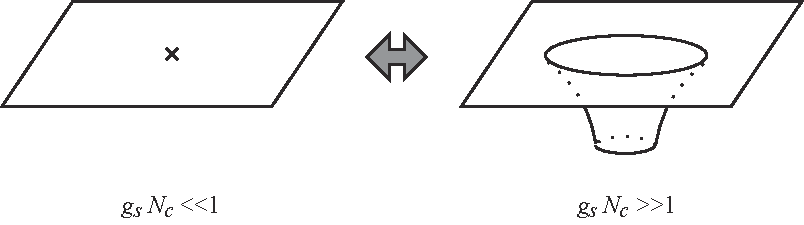
\includegraphics{Ch5_near_horizon_limit.pdf} }
%\scalebox{0.5}{ \includegraphics{Ch5_near_horizon_limit1.pdf} }
\vskip2mm
\caption{When $g_s N_c \ll 1$, the curved spacetime region by the D-brane is small so that one can approximate the geometry by a flat spacetime with a source (left). However, when $g_s N_c \gg 1$, a macroscopic curved spacetime appears (right).}
\label{fig:near_horizon}
\end{figure}%
%%============

The supergravity description is appropriate in the $g_s N_c \gg 1$ limit. The black D3-brane is given by \cite{Horowitz:1991cd}
%It is more convenient to use supergravity to consider such a situation. According to supergravity, the black D3-brane is given by \cite{Horowitz:1991cd}
%curved spacetime made by the D3-brane is given by 
%���̂悤�ȋȂ�����������l����ɂ́C�ނ��뒴�d�͗��_���g�������������D���d�͗��_���g���ƁCD3�u���[���ɂ���č����Ȃ���������̗l�q�́C
\begin{align}
%
ds_{10}^2 &= Z^{-1/2} (- dt^2 + d\bmx_3^2) + Z^{1/2} (dr^2+r^2 d\Omega_5^2)~,
\label{eq:D3_extreme} \\
Z &= 1+\left(\frac{L}{r}\right)^4~, \quad
L^4 \simeq g_s N_c l_s^4~,
\label{eq:D3_extreme2}
%\label{eq:}
%
\end{align}
where $\bmx_3=(x,y,z)$ represents the directions of the spatial extension of the brane. The behavior of the factor $Z$ comes from the Newtonian potential \eqref{eq:Newton_D3}. We are interested in how the D-brane curves the spacetime near the origin. So, taking the limit $r \ll L$ (\keyword{near-horizon limit}), one gets
%�����ŁC$\bmx_3=(x,y,z)$ �̓u���[�����L�тĂ������������킷�D���܁CD�u���[�������_�߂��łǂ�������Ȃ���̂��ɋ���������̂ŁC$r \ll L$ �Ɍ����Ƃ�Ɓi{\bf near-horizon �Ɍ�}\index{near-horizon���悭����@near-horizon �Ɍ�}�j�C
\be
%
ds_{10}^2 \rightarrow \left(\frac{r}{L}\right)^2 (- dt^2 + d\bmx_3^2)
+ L^2 \frac{dr^2}{r^2}+L^2 d\Omega_5^2~.
\label{eq:D3_near_horizon}
%
\ee
The part $L^2 d\Omega_5^2$ represents $S^5$ with radius $L$. The remaining five-dimensional part is the AdS$_5$ spacetime. This near-horizon limit corresponds to the decoupling limit from the gauge theory point of view%
%�Ō�� $L^2 d\Omega_5^2$ �̕����́C���a $L$ �� $S^5$ ������킷�D�c���5�����������CAdS$_5$����ł���D���� near-horizon �Ɍ��́C�Q�[�W���_�̗���ł� decoupling �Ɍ��ɑ�������%
\footnote{
\advanced To see the relation, we need to discuss the decoupling limit more carefully. Denote the typical scale of the gauge theory as $l_\text{obs}$. One can ignore the string length scale $l_s$ when
%�Q�[�W���_�̓T�^�I�ȃX�P�[���� $l_\text{obs}$ �Ƃ���ƁC�������_�̃X�P�[�� $l_s$ �������ł���̂́C
\be
%
l_s \ll l_\text{obs}~.
\label{eq:decoupling1}
%
\ee
As $l_\text{obs}$, let us take the ``W-boson" mass scale. Here, the ``W-boson" is the gauge boson which arises by breaking the gauge group $SU(N_c) \rightarrow SU(N_c-1) \times U(1)$. This corresponds to separating a D-brane from $N_c$ D-branes. The gauge boson corresponds to an open string, but the open string between the D-brane and $(N_c-1)$ D-branes is stretched, and the open string has a tension. So, the corresponding W-boson becomes massive. The mass is given by
%�̏ꍇ�ł���D$l_\text{obs}$ �Ƃ��āuW�{�]���̎��ʃX�P�[���v��I�Ԃ��Ƃɂ��悤�D�����Ō����uW�{�]���v�Ƃ́C�Q�[�W�Q�� $SU(N_c) \rightarrow SU(N_c-1) \times U(1)$ �Ɣj�����Ƃ��̃Q�[�W�{�]���̎��ʂł���DD�u���[���ł́C$N_c$ ���d�Ȃ���D�u���[������1�������i����$r$�j�������Ƃɑ�������D�Q�[�W�{�]���͊J���ɑ����������C���̂悤�ɕ�����ƊJ���͒��͂������Ă���̂ŁC�Q�[�W�{�]���� massive �ɂȂ�D���̎��ʂ�
\be
%
\frac{1}{l_\text{obs}} \simeq \frac{r}{l_s^2} 
\label{eq:gauge_boson}
%
\ee
[The tension of the open string is $O(1/l_s^2)$]. From Eqs.~\eqref{eq:decoupling1} and \eqref{eq:gauge_boson}, one gets
%���x�ɂȂ�i�J���̒��͂� $\simeq 1/l_s^2$�j�D\eq{decoupling1}��\eq{gauge_boson}����
\be
%
r \ll l_s~.
\label{eq:decoupling2}
%
\ee
This is the decoupling limit. 
%�Ƃ����֌W��������D���ꂪ decoupling �Ɍ��ł���D

When $g_s N_c \gg 1$, the $r \ll l_s$ limit implies $r \ll L$, which is the near-horizon limit. 
%$g_s N_c \gg 1$ �̏ꍇ�C$r \ll l_s$ �Ɍ��� $r \ll L$�� near-horizon�Ɍ����Ӗ�����D
}.

Therefore, let us roughly divide the spacetime made by the D3-brane into AdS$_5 \times S^5$ near the origin and the nearly flat spacetime around:
%�ȏ���CD3�u���[������鎞���傴���ςɌ��_�߂��� AdS$_5 \times S^5$ �Ƃ��̎���̕��R�Ȏ���ɕ����邱�Ƃɂ��悤�F
\begin{center}
(supergravity on AdS$_5 \times S^5$) \\ + (supergravity in the 10-dimensional flat spacetime)
%�iAdS$_5 \times S^5$ ��̒��d�͗��_�j\\�{�i���R��10���������̒��d�͗��_�j
\end{center}

As we will see in \chap{AdS}, the AdS$_5$ spacetime has the $SO(2,4)$ invariance. In addition, the full geometry \eqref{eq:D3_near_horizon} involves $S^5$ which has the $SO(6)$ invariance. This is the same symmetry as the ${\cal N}=4$ R-symmetry. Thus,
%\sect{scale_inv}�łӂꂽ�悤�ɁCAdS$_5$ ����� $SO(2,4)$ �Ώ̐������D���킦�āC�v�� \eqref{eq:D3_near_horizon} �� $S^5$ ���܂ނ̂ŁC ${\cal N}=4$ R�Ώ̐��Ɠ��� $SO(6)$ �Ώ̐������D���������āC
\begin{center}
\fbox{
\begin{tabular}{l}
The gravity side also has the global $SO(2,4) \times SO(6)$ symmetry.
%�d�͑���$SO(2,4) \times SO(6)$ ���I�Ώ̐�������
\end{tabular}
}
\end{center}

The gauge theory description fails when $g_s N_c \gg 1$. On the other hand, the supergravity description fails when $g_s N_c \ll 1$. This is because the curvature of the metric \eqref{eq:D3_near_horizon} behaves as
% ���F���b�`�X�J���[����S^5�����Ƃ��킹�ă[���ɂȂ�
\be
%
R^{MNPQ} R_{MNPQ} \propto \frac{1}{g_s N_c l_s^4}~.
%\label{eq:}
%
\ee
When $g_s N_c \ll 1$, the curvature becomes large. The $\alpha'$-corrections \index{alpha'-corrections@$\alpha'$-corrections} become important, which can change the metric \eqref{eq:D3_near_horizon} in general. The metric such as \eq{D3_near_horizon} is trustable when $g_s N_c \gg 1$. 


%%============
\begin{figure}[tb]
\centering
\subfigure[${\cal N}=4$ SYM]{
\scalebox{0.75}{ 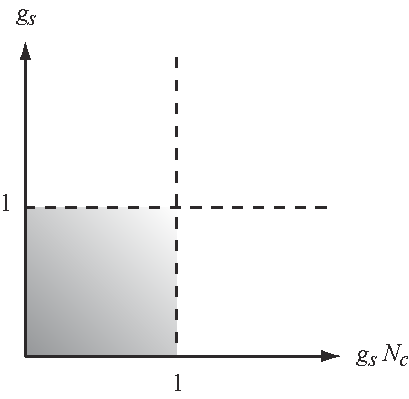
\includegraphics{Ch5_ads_cft1.pdf} }
} 
\subfigure[Supergravity on AdS$_5 \times S^5$]{
\scalebox{0.75}{ 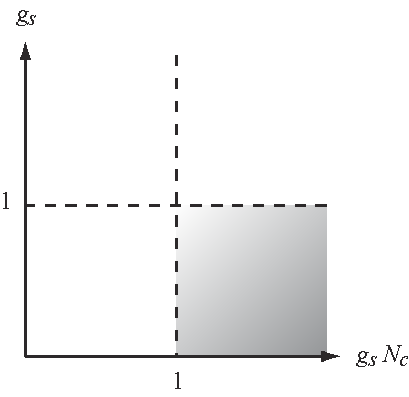
\includegraphics{Ch5_ads_cft2.pdf} }
}
\vskip2mm
\caption{
We obtained two systems from the D3-brane, the \Nfour\ SYM and supergravity on  AdS$_5 \times S^5$. These two theories are complementary to each other. Each theory has a region where analysis is relatively easy (shaded region), but they do not overlap. AdS/CFT claims that two systems are equivalent.
%D3�u���[������ \Nfour �Q�[�W���_�� AdS$_5 \times S^5$ ��̒��d�͗��_������ꂽ���C2�‚̗��_�͑���I�Ȋ֌W�ɂ���D���Ȃ킿�C���ꂼ��̗��_�ʼn�͂��e�Ղȗ̈�i�A�~�������������j�͏d�Ȃ�Ȃ��DAdS/CFT�͂��̗��҂��������Ǝ咣����D
}
\label{fig:ads_cft}
\end{figure}%
%%============


%%-------------------------------------
\subsection{Gauge theory and curved spacetime
%�Q�[�W���_�ƋȂ���������
}%\label{sec:bh}
%%-------------------------------------

To summarize our discussion so far, we obtained two systems from the D3-brane, the \Nfour\ SYM and supergravity on AdS$_5 \times S^5$. We also obtained a common system which is decoupled from the rest, supergravity in the 10-dimensional flat spacetime, in both cases. Since this part is common, one can forget it. Then, the \Nfour\ SYM corresponds to supergravity on AdS$_5 \times S^5$. 
%����܂ł̋c�_���܂Ƃ߂�ƁCD3�u���[������ \Nfour �Q�[�W���_�� AdS$_5 \times S^5$ ��̒��d�͗��_��2�‚̌n������ꂽ�D�܂��C���R��10���������̒��d�͗��_���������ʂ��Ă����ꂽ�D���̕����͋��ʂ��Ă���̂ŁC�c��̕����C\Nfour �Q�[�W���_�� AdS$_5 \times S^5$ ��̒��d�͗��_������Ӗ��Ή����Ă��邱�ƂɂȂ�D

These two descriptions of the brane, gauge theory and supergravity, are complementary to each other (\fig{ads_cft}). %As we saw earlier, 
The former description is valid when $g_s \ll 1$ and $g_s N_c \ll 1$, whereas the latter description is valid when $g_s \ll 1$ and $g_s N_c \gg 1$. 
%This is because the curvature of the metric \eqref{eq:D3_near_horizon} behaves as
%�����Ƃ��C�Q�[�W���_�ɂ��u���[���`���ƁC���d�͗��_�ɂ��u���[���`���Ƃ́C����I�Ȋ֌W�ɂ���i\fig{ads_cft}�j�D�����ɂ݂��悤�ɕ��R�Ȏ���ł̕`���́C$g_s \ll 1$�C$g_s N_c \ll 1$ �̂Ƃ��ɐ������邪�C���d�͗��_�ɂ��`���� $g_s \ll 1$�C$g_s N_c \gg 1$ �̂Ƃ��ɐ�������D�v�� \eqref{eq:D3_near_horizon} �ɑ΂��āC�ȗ���
% ���F���b�`�X�J���[����S^5�����Ƃ��킹�ă[���ɂȂ�
%\be
%
%R^{MNPQ} R_{MNPQ} \propto \frac{1}{g_s N_c l_s^4}~.
%\label{eq:}
%
%\ee
%When $g_s N_c \ll 1$, the curvature becomes large. The $\alpha'$-corrections \index{alpha'-corrections@$\alpha'$-corrections} become important, which can change the metric \eqref{eq:D3_near_horizon} in general. The metric such as \eq{D3_near_horizon} is trustable when $g_s N_c \gg 1$. 
%�ƐU��܂�����ł���D$g_s N_c \ll 1$ �̂Ƃ��͎���̋ȗ����傫���Ȃ�D���̂Ƃ���$\alpha'$�␳\index{alpha'�ق���@$\alpha'$�␳}�����������C��ʂɌv�� \eqref{eq:D3_near_horizon} �̗l�q�͑傫���ς�肤��D�‚܂�C\eqref{eq:D3_near_horizon} �̂悤�Ȍv�ʂ���ʂɐM���ł���̂́C$g_s N_c \gg 1$ �̂Ƃ��ł���D

However, in principle, both theories exist for all $g_s$ and $g_s N_c$. Taking \sect{reexamination} discussion into account, it is natural to imagine that both theories are equivalent for all $g_s$ and $g_s N_c$. If this is true, we can make computations using one theory even when the other theory is hard to compute. 
%�������C�����I�ɂ͂ǂ���̗��_�� $g_s$�C$g_s N_c$ �̑S�̈�ő��݂���D\sect{reexamination}�̋c�_�𓥂܂���ƁC���҂̗��_�� $g_s$�C$g_s N_c$ �̑S�̈�œ����ł���ƍl����̂����R�ł���D���Ƃ���ƁC����̗��_�ʼn�͂�����̈�ł��C��������̗��_���g���Čv�Z�ł��邱�ƂɂȂ�D

We should stress that this is not a logical consequence. We obtained two systems from the D3-brane. But these two systems are two different limits of the brane. In order to justify the above claim, one has to compare results in both theories computed at the same $g_s$ and $g_s N_c$. There are many circumstantial evidences when one can rely on supersymmetry, but we will not discuss such evidences in this book. Rather, we go through computations related to actual applications, and we will see that gravity results can indeed be interpreted as physical quantities of gauge theories. We also compare the AdS/CFT results with experiments and with the other theoretical tools such as the lattice gauge theory in order to see that AdS/CFT is likely to be true.
%����͘_���I�ȋA���Ƃ����킯�ł͂Ȃ��D2�‚̗��_��D3�u���[�����瓾��ꂽ�D�������CD3�u���[���̈Ⴄ�Ɍ���2�‚̗��_�ɑΉ�����ɂ����Ȃ�����ł���D���������āC���̎咣���m���߂�ɂ́C����  $g_s$�C$g_s N_c$ �ŗ����̌��ʂ��ׂ邱�Ƃ��K�v�ł���D���Ώ̐������݂���󋵉��ł́C�����̏󋵏؋��������Ă���D�������C�{���ł͂��̂悤�ȏ؋��͋c�_���Ȃ��D�ނ���C���ۂ̉��p�Ɋ֌W�����v�Z��ʂ��āC�d�͗��_����Q�[�W���_�Ƃ��Ď��R�ɉ��߂ł��镨���ʂ��o�Ă��邱�Ƃ�C�������ʂ�ق��̗��_�I��@�œ���ꂽ���ʁi�i�q�Q�[�W���_�Ȃǁj�Ɣ�ׂ邱�ƂŁCAdS/CFT���m���炵�����Ƃ��݂���j���Ƃ�D


%%-------------------------------------
\subsection{What D-brane tells us
%D�u���[����ʂ��Ă킩��������
}\label{sec:definition}
%%-------------------------------------

The D-brane taught us two things. First, the GKP-Witten relation \eqref{eq:pre_GKPW2} becomes more precise:
%D�u���[����ʂ��Ă킩�������ƂƂ��āC����GKP-�E�B�b�e���֌W��\eqref{eq:pre_GKPW2}�̗��ӂ���萳�m�ɂ킩�������Ƃ���������F
\be
%
%\boxeq{
Z_\text{\Nfour} = Z_\text{AdS$_5 \times S^5$}~.
%}
%\label{eq:
%
\ee
The left-hand side is the partition function of the \Nfour\ SYM, and the right-hand side is the partition function of string theory on AdS$_5 \times S^5$. 
%���ӂ�\Nfour �Q�[�W���_�̕��z�֐��C�E�ӂ�AdS$_5 \times S^5$����ł̒������_�̕��z�֐��ł���D

We mainly focused on the conformal invariance. But, in retrospect, we are able to identify the gauge theory because we take the \Nfour\ R-symmetry into account. One would say that we added $S^5$ on the gravity side to reflect the R-symmetry on the gauge theory side. Thus, when we try to find a gravity dual, it is in general important to take care of the symmetries both theories have.
%����܂ŃR���t�H�[�}���Ώ̐������ɒ��ڂ������C���_�����ł����̂́C���ǂ̂Ƃ���${\cal N}=4$ R�Ώ̐����l���������߂ł���D���̑Ώ̐��𔽉f�����邽�߁C�d�͑��ɂ�$S^5$���‚��������Ƃ�������D���������āC${\cal N}=4$ �Q�[�W���_�ȊO�̏ꍇ�ŁC�Ή�����d�͗��_���݂‚���ۂɂ��C�o���̗��_�����‘Ώ̐��𐶂������Ƃ��d�v�ł���D

Second, from the D-brane, we are able to obtain the AdS/CFT dictionary \eqref{eq:dictionary_preview}. This is possible by combining various expressions we encountered:
%���ɂ킩�邱�ƂƂ��ẮC�����_�̃p�����[�^�̊֌W\eqref{eq:pre_dictionary}�ł���D����́C����܂łɓo�ꂵ����~\eqref{eq:string_vs_qft}, \eqref{eq:D3_extreme2} ���܂Ƃ߂邱�Ƃœ�����F
%\begin{subequations}
%\label{eq:}
\begin{align}
%
L^4 &\simeq g_s N_c l_s^4~, \\
G_{10} %&\simeq& G_5 L^5 
&\simeq g_s^2 l_s^8~, \\
g_s &\simeq g_\text{YM}^2~.
%\label{eq:}
%
\end{align}
%\end{subequations}
Eliminating $g_s$ from these expressions give
%�����̎����� $g_s$ ����������ƁC
\be
%
N_c^2 \simeq \frac{L^8}{G_{10}}~, \quad \lambda \simeq \left(\frac{L}{l_s} \right)^4~.
\label{eq:dictionary_preliminary}
%
\ee
%������{\bf AdS/CFT����}\index{AdS/CFT������@AdS/CFT����}�ƌĂ΂�鎮��1�‚ł���D

Now, $S^5$ corresponds to the R-symmetry from the point of view of the \Nfour\ SYM and is an important part of the theory. But one often compactifies $S^5$ and consider the resulting five-dimensional gravitational theory. The theory obtained in this way is called \keyword{gauged supergravity}.
%���āC$S^5$ �� \Nfour �Q�[�W���_�̗���ł�R�Ώ̐��ɑ��������_�̏d�v�Ȉꕔ�����C���΂��� $S^5$ ���R���p�N�g�����āC����5�����̏d�͗��_���l����D�������ē���ꂽ���_��{\bf �Q�[�W�����ꂽ���d�͗��_}\index{���[�������ꂽ���悤���䂤��悭����@�Q�[�W�����ꂽ���d�͗��_}�igauged supergravity�j�ƌĂ΂��D

The actual procedure of the $S^5$ compactification is rather complicated, and the full gauged supergravity action is complicated as well. But in our case, we do not have to go through such a computation, and we can infer the action. The five-dimensional part is the AdS$_5$ spacetime, so the five-dimensional action should be given by \eq{gravity_side}. Since $S^5$ has radius $L$, the compactification gives
%���̃R���p�N�g���̎葱���͎��ۂɂ͕��G�ŁC�������p�����G�����C���܂̏ꍇ�͎��ۂɂ����Ȃ��K�v�͂Ȃ��C������x�������‚��D�ƌ����̂��C5���������� AdS$_5$ ����Ȃ̂ŁC5������p��\eq{gravity_side}�ŗ^������͂��ł���D$S^5$ �̔��a�� $L$ �Ȃ̂ŁC�R���p�N�g���ɂ����
\be
%
\frac{1}{16\pi G_{10}} \int d^{10}x \sqrt{-g_{10}}R_{10} 
=
\frac{L^5 \Omega_5}{16\pi G_{10}} \int d^{5}x \sqrt{-g_{5}}\left(R_{5} 
%+ O\left(\frac{1}{L^2}\right)  
+\cdots \right)~.  
\nonumber
%\label{eq:G10_vs_G5}
%
\ee
Thus, the five-dimensional Newton's constant is given by  $G_5 \simeq G_{10}/L^5$. Then, the AdS/CFT dictionary \eqref{eq:dictionary_preliminary} can be rewritten by $G_5$. If one works out numerical coefficients, the results are
%���������āC5�����̃j���[�g���萔�� $G_5 \simeq G_{10}/L^5$ �ł���D������g���ƁCAdS���� \eqref{eq:dictionary_preliminary} �� $G_5$ �ŏ����������Ƃ��ł���D�W���܂Œ��ӂ��Ă܂Ƃ߂�ƁC
\be
%
\boxeq{
N_c^2 = \frac{\pi}{2} \frac{L^3}{G_5}~, \quad
\lambda = \left(\frac{L}{l_s}\right)^4~.
}
\label{eq:dictionary}
%
\ee

%%-------------------------------------
\subsubsection*{Finite-temperature case
%�L�����x�̏ꍇ
}
%%-------------------------------------


The metric \eqref{eq:D3_extreme} is the zero-temperature solution of the D3-brane, or the extreme black hole \index{extreme black hole} solution, which corresponds to the \Nfour\ SYM at zero temperature. In order to discuss the finite temperature gauge theory, we use the finite temperature solution of the D3-brane:
%\eq{D3_extreme} ��D3�u���[���̃[�����x�̉��i�Ɍ��u���b�N�z�[��\index{���悭����ӂ�‚��ف[��@�Ɍ��u���b�N�z�[��}�j�ł���C�[�����x��\Nfour �Q�[�W���_�ɑ�������D�L�����x���l����ɂ́CD3�u���[���̗L�����x�����g���F
%\begin{subequations}
%\label{eq:}
\begin{align}
%
ds_{10}^2 &= Z^{-1/2} (- h dt^2 + d\bmx_3^2) + Z^{1/2} (h^{-1}dr^2+r^2 d\Omega_5^2)~,
\\
Z &= 1+\left(\frac{L}{r}\right)^4~, \\
h &= 1-\left(\frac{r_0}{r}\right)^4~. 
\label{eq:D3_non_extreme}
%\label{eq:}
%
\end{align}
%\end{subequations}
The horizon is located at $r=r_0$. Again take the near-horizon limit $r \ll L$. In order to remain outside the horizon $r > r_0$ even in the near-horizon limit, take $r_0 \ll L$. Then, the resulting geometry is
%$r=r_0$ ���z���C�Y���ł���Dnear-horizon �Ɍ� $r \ll L$ ���Ƃ��Ă��C�z���C�Y���̊O�ł��邽�߂�$r_0 \ll L$�Ƃ���D����ƁCnear-horizon �Ɍ��ŁC
\be
%
ds_{10}^2 \rightarrow \left(\frac{r}{L}\right)^2 (- h dt^2 + d\bmx_3^2)
+ L^2 \frac{dr^2}{hr^2}+L^2 d\Omega_5^2~.
\label{eq:D3_near_horizon2}
%
\ee
This is known as the \textit{Schwarzschild-AdS$_5$ black hole}\index{Schwarzschild-AdS black hole (planar horizon)} (\chap{AdS_BH}). When $h=1$, the geometry reduces to the AdS$_5$ spacetime. Also, the factor similar to $h$ appeared in the higher-dimensional Schwarzschild black holes.
%����́C�V�������c�V���hAdS$_5$ �u���b�N�z�[��\index{������‚����AdS�ӂ�‚��ف[��ӂ�ȁ[�ق炢����@�V�������c�V���hAdS�u���b�N�z�[���i�v���i�[�E�z���C�Y���j}�ƌĂ΂����ł���i\chap{AdS_BH}�j�D$h=1$�̏ꍇ��AdS$_5$�v�ʂł���C$h$�Ƃ������q�͍������V�������c�V���h�E�u���b�N�z�[���Ǝ��Ă���D

% omitted from Springer edition
%%-------------------------------------
%\subsubsection*{Comment}
%%-------------------------------------

%Just to make sure, string theory is the prime candidate of the unified theory, but string theory in AdS/CFT is not the one as the unified theory but rather an ``artificial" string theory. In the real world, the Newton's constant is fixed, so string theory as the unified theory should predict the value%
%\footnote{This is part of the so-called ``moduli problem" and the detailed mechanism is not known yet.}.
%Hence, one cannot take the $N_c\rightarrow\infty$ limit in reality. In AdS/CFT, we consider an artificial string theory in order to represent large-$N_c$ gauge theories. 
%�O�̂��߂ɒ��ӂ��Ă����ƁC�������_�͓��ꗝ�_�̍ŗL�͌�₾���CAdS/CFT�ōl����͓̂��ꗝ�_�Ƃ��Ă̒������_�ł͂Ȃ��C�u���z�I�ȁv�������_�ł���D�ƌ����̂́C���Ƃ��Ό������E�ł̓j���[�g���萔$G$�͌��܂��Ă���̂ŁC�����I�Ȓ������_�ł� $N_c\rightarrow\infty$�Ɍ��͂Ƃꂸ�C����l�ɒ�܂��Ă���͂�������ł���%
%\footnote{���̃��J�j�Y���ɂ‚��ẮC�܂��ڂ������Ƃ͂킩���Ă��Ȃ��D}�D
%AdS/CFT�ōl����̂́C���[�W$N_c$�Q�[�W���_������킷���߂̉��z�I�Ȓ������_�ł���D

\endofsection

	   \begin{thebibliography}{99}

%
% Chap_string 
%

%\cite{Donnachie:2002en}
\bibitem{Donnachie:2002en}
  S.~Donnachie, H.~G.~Dosch, O.~Nachtmann and P.~Landshoff,
  \textit{Pomeron physics and QCD} (Cambridge Univ.\ Press, %Cambridge, 
  2002).

%\cite{Chew:1962eu}
\bibitem{Chew:1962eu}
  G.~F.~Chew and S.~C.~Frautschi,
  ``Regge Trajectories And The Principle Of Maximum Strength For Strong Interactions,''
  Phys.\ Rev.\ Lett.\  {\bf 8 } (1962)  41.

% added
%\cite{Dai:1989ua}
\bibitem{Dai:1989ua}
  J.~Dai, R.~G.~Leigh and J.~Polchinski,
  ``New Connections Between String Theories,''
  Mod.\ Phys.\ Lett.\ A {\bf 4} (1989) 2073.
  %%CITATION = MPLAE,A4,2073;%%

% added
%\cite{Polchinski:1995mt}
\bibitem{Polchinski:1995mt}
  J.~Polchinski,
  ``Dirichlet Branes and Ramond-Ramond charges,''
  Phys.\ Rev.\ Lett.\  {\bf 75} (1995) 4724
  [hep-th/9510017].
  %%CITATION = HEP-TH/9510017;%%

%\cite{Sakai:2004cn}
\bibitem{Sakai:2004cn}
  T.~Sakai and S.~Sugimoto,
  ``Low energy hadron physics in holographic QCD,''
  Prog.\ Theor.\ Phys.\  {\bf 113} (2005) 843
  [hep-th/0412141].
  %%CITATION = HEP-TH/0412141;%%
  
% added
%\cite{Freedman:2012zz}
\bibitem{Freedman:2012zz}
  D.~Z.~Freedman and A.~Van Proeyen, \textit{Supergravity} (Cambridge Univ.\ Press, 2012).

% added
%\cite{Polchinski:1992ed}
\bibitem{Polchinski:1992ed}
  J.~Polchinski,
  ``Effective field theory and the Fermi surface,'' TASI1992
%In *Boulder 1992, Proceedings, Recent directions in particle theory* 235-274, and Calif. Univ. Santa Barbara - NSF-ITP-92-132 (92,rec.Nov.) 39 p. (220633) Texas Univ. Austin - UTTG-92-20 (92,rec.Nov.) 39 p
  [hep-th/9210046].
  %%CITATION = HEP-TH/9210046;%%

% added
%\cite{Polyakov:1981rd}
\bibitem{Polyakov:1981rd}
  A.~M.~Polyakov,
  ``Quantum Geometry of Bosonic Strings,''
  Phys.\ Lett.\ B {\bf 103} (1981) 207.
  %%CITATION = PHLTA,B103,207;%%
 
% added
%\cite{Natsuume:1992ky}
\bibitem{Natsuume:1992ky}
  M.~Natsuume,
  ``Nonlinear sigma model for string solitons,''
  Phys.\ Rev.\ D {\bf 48} (1993) 835
  [hep-th/9206062].
  %%CITATION = HEP-TH/9206062;%%

% added
% again
%\cite{Srednicki:2007qs}
\bibitem{Srednicki:2007qs2}
  M.~Srednicki,
  \textit{Quantum field theory}
  (Cambridge Univ.\ Press, 2007).

%\cite{Polchinski:1987dy}
\bibitem{Polchinski:1987dy}
  J.~Polchinski,
  ``Scale and conformal invariance in quantum field theory,''
  Nucl.\ Phys.\  B {\bf 303} (1988) 226.
  %%CITATION = NUPHA,B303,226;%%

%\cite{Gubser:1998bc}
\bibitem{Gubser:1998bc}
  S.~S.~Gubser, I.~R.~Klebanov and A.~M.~Polyakov,
  ``Gauge theory correlators from noncritical string theory,''
  Phys.\ Lett.\  {\bf B428 } (1998)  105
  [hep-th/9802109].
  
%\cite{Witten:1998qj}
\bibitem{Witten:1998qj}
  E.~Witten,
  ``Anti-de Sitter space and holography,''
  Adv.\ Theor.\ Math.\ Phys.\  {\bf 2 } (1998)  253
  [hep-th/9802150].

% again
%\cite{Kiritsis:2007zz}
\bibitem{Kiritsis:2007zz2}
  E.~Kiritsis,
  \textit{String theory in a nutshell}
  (Princeton Univ.\ Press, 2007).

% again
%\cite{Wald:1984rg}
\bibitem{Wald:1984rg2}
R.~M.~Wald,
\textit{General relativity}
(The Univ.\ of Chicago Press, 1984).

%\cite{Baier:2007ix}
\bibitem{Baier:2007ix}
  R.~Baier, P.~Romatschke, D.~T.~Son, A.~O.~Starinets and M.~A.~Stephanov,
  ``Relativistic viscous hydrodynamics, conformal invariance, and holography,''
  JHEP {\bf 0804} (2008) 100
  [arXiv:0712.2451 [hep-th]].
  %%CITATION = JHEPA,0804,100;%%

% added
%\cite{Horowitz:1991cd}
\bibitem{Horowitz:1991cd}
  G.~T.~Horowitz and A.~Strominger,
  ``Black strings and P-branes,''
  Nucl.\ Phys.\ B {\bf 360} (1991) 197.
  %%CITATION = NUPHA,B360,197;%%

\end{thebibliography}
	%\documentclass[11pt]{jarticle} %%% �A���R�����g
\ifx\nameofpaper\undefined %%% ���� main.tex ���ǂ܂�Ă��Ȃ����
  \usepackage{macro_natsuume} %%% �����p�̃}�N���t�@�C����ǂݍ��݁C
  \def\beginsection{\section*}
  \def\endofsection{\end{document}} %%% \endofsection = \bye �ƒ�`
  \input draft_header.tex
\else %%% �����łȂ����
  \def\beginsection{\chapter}
  \def\endofsection{\endinput} %%% \endofsection = \endinput �ƒ�`
\fi


%%%%%%%%%
\beginsection{The AdS spacetime}\label{chap:AdS}
%%%%%%%%%

%\begin{flushright}
%        \today\\
%\end{flushright}

\begin{quote}
The AdS spacetime is one of spacetimes with constant curvature. To be familiar with the AdS spacetime, we first discuss spaces with constant curvature such as the sphere and then discuss spacetimes with constant curvature.
%AdS����͒�ȗ�����ƌĂ΂�鎞��̈��ł���D�Ȃ��݂����‚��߂ɁC�܂����̂悤�Ȓ�ȗ���Ԃ��c�_���C����𓥂܂��Ē�ȗ�������c�_����D
\end{quote}

%%%%%%%%%
\section{Spacetimes with constant curvature}%\label{sec}
%%%%%%%%%

%%------------------
\subsection{Spaces with constant curvature}%\label{sec:}
%%------------------

Before we discuss spacetimes with constant curvature such as the AdS spacetime, let us consider a simple example, the sphere $S^2$. Consider the three-dimensional Euclidean space with metric
%AdS����̂悤�Ȓ�ȗ�������c�_����O�ɁC�܂��͊ȒP�ȗ�C2������$S^2$����l���悤�D����3�������[�N���b�h���
\be
%
ds^2 = dX^2 + dY^2 + dZ^2~.
\label{eq:embed_s2}
%
\ee
The sphere is defined by the surface which satisfies the constraint
%�̂Ȃ��ŁC
\be
%
X^2 + Y^2 + Z^2 = L^2~.
\label{eq:surface_s2}
%
\ee
This constraint can be solved by the familiar spherical coordinates:
%�Ƃ��������𖞂����ʂƂ��Ē�`�����D���̍S�������͕W���I�ȋɍ��W���g�����Ƃʼn������Ƃ��ł���F
\be
%
X = L \sin\theta \cos\varphi~, \quad Y = L \sin\theta \sin\varphi~, \quad Z = L \cos\theta~.
%
\ee
In this coordinate system, the metric then becomes 
%���̍��W�Ōv�ʂ�
\be
%
ds^2 = L^2(d\theta^2 + \sin^2\theta\, d\varphi^2)~.
\label{eq:metric_s2}
%
\ee
%The sphere $S^2$ is homogeneous and isotropic. This is because the surface \eqref{eq:surface_s2} respects the $SO(3)$ invariance of the ``ambient space," the three-dimensional Euclidean space \eqref{eq:embed_s2}. Namely, any point on $S^2$ can be mapped to the other points by an $SO(3)$ transformation. 
The sphere $S^2$ has the $SO(3)$ invariance. This is because the surface \eqref{eq:surface_s2} respects the $SO(3)$ invariance of the ``ambient space," the three-dimensional Euclidean space \eqref{eq:embed_s2}. By an $SO(3)$ transformation, any point on $S^2$ can be mapped to the other points. In this sense, $S^2$ is homogeneous. The sphere has a constant positive curvature and the Ricci scalar is given by
%$S^2$ �͈�l�ȋ�Ԃł���D����́C�� \eqref{eq:surface_s2} ��3�������[�N���b�h���  \eqref{eq:embed_s2} �̑Ώ̐� $SO(3)$ ��ۂ‚��Ƃ���킩��D�‚܂�C$S^2$ �̂ǂ̓_�� $SO(3)$ �ϊ��ɂ���āC�ق��̓_�Ɉڂ邱�Ƃ��ł���D���̋ȗ��͐��̒萔�������C���b�`�E�X�J���[��
\be
%
R = \frac{2}{L^2}~.
%
\ee

%%============
\begin{figure}[tb]
\centering
%\hspace{0.25in}
\scalebox{0.75}{  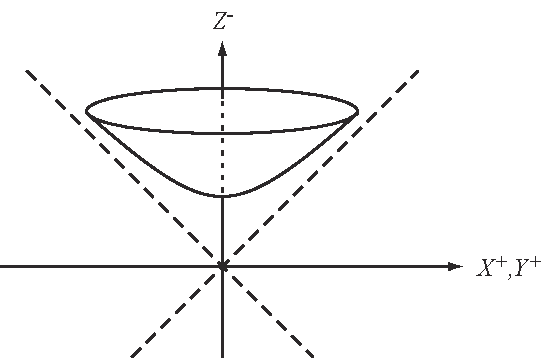
\includegraphics{Ch6_H2.pdf} }
\vskip2mm
\caption{The embedding of $H^2$ into $\mathbb{R}^{1,2}$. The superscript signs refer to the signature of the ambient spacetime ($-$: timelike, $+$: spacelike).}
%�o�ȋ�� H$^2$ �� $\mathbb{R}^{1,2}$ �ւ̖��ߍ��݁D���W�̌��̕����́C�e���W�����ԓI�i$-$�j����ԓI�i$+$�j��������킷�D}
\label{fig:H2}
\end{figure}%
%%============

The space with constant negative curvature is known as the \keyword{hyperbolic space} $H^2$. It is much harder to visualize the space with constant negative curvature. It is partly because the hyperbolic space cannot be embedded into the three-dimensional Euclidean space unlike the sphere. But the hyperbolic space can be embedded into the three-dimensional Minkowski space. The hyperbolic space is defined by
%����C���̒�ȗ�����������Ԃ́C{\bf �o�ȋ��}\index{�������悭��������@�o�ȋ��}�iH$^2$�j�Ƃ��Ēm���Ă���D���̒�ȗ�����������Ԃ́C�����ƃC���[�W������ł���D��‚̗��R�́C�o�ȋ�Ԃ͋��ƈႢ�C3�����̃��[�N���b�h��Ԃɂ͖��ߍ��ނ��Ƃ��ł��Ȃ�����ł���D�������C3�����̃~���R�t�X�L�[��Ԃɂ͖��ߍ��ނ��Ƃ��ł���D�o�ȋ�Ԃ́i\fig{H2}�j�C
\begin{gather}
%
ds^2 = - dZ^2 + dX^2 + dY^2~,
\label{eq:embed_h2} \\
-Z^2 + X^2 + Y^2 = - L^2~,
\label{eq:surface_h2}
%
\end{gather}
(\fig{H2}). The hyperbolic space is homogeneous in the sense that it respects the $SO(1,2)$ invariance of the ambient Minkowski spacetime. Namely, any point on the surface can be mapped to the other points by an $SO(1,2)$ ``Lorentz" transformation. Note that the hyperbolic space is \textit{not} the familiar hyperboloid in the three-dimensional Euclidean space:
%�Ƃ��Ē�`�����D�o�ȋ�Ԃ͌v�ʂ̑Ώ̐� $SO(1,2)$ ��ۂˆ�l�ȋ�Ԃł���D�‚܂�C�ʏ�̂ǂ̓_��$SO(1,2)$�u���[�����c�ϊ��v�ɂ���āC�ق��̓_�Ɉڂ邱�Ƃ��ł���D�܂��C�o�ȋ�Ԃ͑o�Ȗʁihyperboloid�j�ł͂Ȃ����Ƃɒ��ӁF
\begin{gather}
%
ds^2 = dZ^2 + dX^2 + dY^2~, \\
-Z^2 + X^2 + Y^2 = - L^2~.
%
\end{gather}
The hyperboloid is embedded into the three-dimensional Euclidean space. Thus, the hyperboloid does not respect the $SO(3)$ invariance of the ambient space, and it is not homogeneous.
%�o�Ȗʂ̓��[�N���b�h��Ԃɖ��ߍ��܂�Ă���C�v�ʂ̑Ώ̐� $SO(3)$ ��ۂ��Ȃ��D���Ȃ킿�C�o�Ȗʂ͈�l�ȋ�Ԃł͂Ȃ��D 

In order to solve the constraint \eqref{eq:surface_h2}, take a coordinate system which is slightly different from the sphere:
%�S������ \eqref{eq:surface_h2} ���������߂ɁC���̏ꍇ�Ə����Ⴄ���W�n���Ƃ�F
\be
%
X = L \sinh\rho \cos\varphi~, \quad Y = L \sinh\rho \sin\varphi~, \quad Z = L \cosh\rho~.
%
\ee
Then, the metric of the hyperbolic space is given by
%����ƁC�o�ȋ�Ԃ̌v�ʂ́C
\be
%
ds^2 = L^2 (d\rho^2 + \sinh^2\rho\, d\varphi^2)~.
\label{eq:metric_h2}
%
\ee
As one can see from this metric, the hyperbolic space itself does not have a timelike direction although we embed it into the three-dimensional Minkowski spacetime. Namely, the hyperbolic space is a space not a spacetime. The curvature is constant negative:
%�v�ʂ��݂�΂킩��悤�ɁC3�����̃~���R�t�X�L�[��Ԃɖ��ߍ���ł�����̂́C�o�ȋ�Ԏ��͎̂��ԕ����������Ȃ����Ƃɒ��ӁD���Ȃ킿�C�o�ȋ�Ԃ͋�Ԃł��莞��ł͂Ȃ��D�ȗ��͕��̒萔�����F
\be
%
R = - \frac{2}{L^2}~.
%
\ee

It is not easy to visualize the hyperbolic space, but there is a familiar example. The mass-shell condition \eqref{eq:constraint_on_shell} in special relativity is nothing but the hyperbolic space. For the particle with mass $m$, the canonical momentum $p_\mu=(p_0,p_1,p_2)$ satisfies
%�o�ȋ�Ԃ��C���[�W����̂͗e�Ղł͂Ȃ����C���ꑊ�Θ_�ɂ����鎿�ʊk���� \eqref{eq:constraint_on_shell} ���o�ȋ�Ԃɂق��Ȃ�Ȃ��D���ω^���� $p^\mu=(p_0,p_1,p_2)$�����Ž��� $m$ �̗��q�ɑ΂��āC
\be
%
p^2 = - (p_0)^2 + (p_1)^2 + (p_2)^2 = - m^2~.
%
\ee
This takes the same from as the embedding equation \eqref{eq:surface_h2} for $H^2$.
%�����藧�‚��C����͑o�ȋ�Ԃ̖��ߍ��ݏ���  \eqref{eq:surface_h2} �Ɠ����`�����Ă���D

%%------------------
\subsection{Spacetimes with constant curvature
%��ȗ�����F�F����������������
}%\label{sec:}
%%------------------

%%============
\begin{figure}[tb]
\centering
%\hspace{0.25in}
\scalebox{0.75}{ 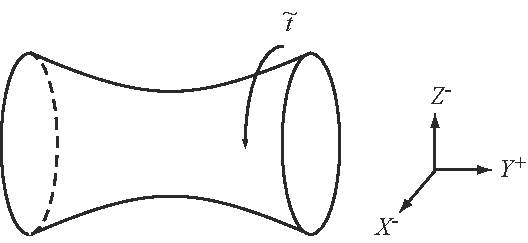
\includegraphics{Ch6_AdS2.pdf} }
\vskip2mm
\caption{The embedding of AdS$_2$ into $\mathbb{R}^{2,1}$. The timelike direction $\tg$ is periodic, so we consider the covering space. }
%AdS$_2$ ����� $\mathbb{R}^{2,1}$ �ւ̖��ߍ��݁D���ԕ����������I�ɂȂ��Ă��邽�߁C�핢��Ԃ��l����D}
\label{fig:AdS2}
\end{figure}%
%%============

So far we discussed spaces with constant curvature, but now consider \textit{spacetimes} with constant curvature. The AdS$_2$ spacetime\index{AdS spacetime} can be embedded into a flat spacetime with \textit{two} timelike directions (\fig{AdS2}):
%����܂ł̋c�_�͒�ȗ����������u��ԁv���������C���悢���ȗ����������u����v���l���悤�D���ԕ�����2�‚��鎞��ɖ��ߍ��ނƁCAdS$_2$����\index{�͂�Ƃ��‚��[������@���h�E�W�b�^�[����}�́i\fig{AdS2}�j
\begin{gather}
%
ds^2 = - dZ^2 - dX^2 + dY^2~,
%ds^2 = - dX^2 - dY^2 + dZ^2~,
\label{eq:embed_ads2} \\
-Z^2 - X^2 + Y^2 = - L^2~.
%-X^2 - Y^2 + Z^2 = - L^2~.
\label{eq:surface_ads2}
%
\end{gather}
The parameter $L$ is called the \keyword{AdS radius}. The AdS$_2$ spacetime has the $SO(2,1)$ invariance. Just like $S^2$ and $H^2$, take a coordinate system
%���̏ꍇ��$L$��{\bf AdS���a}\index{AdS�͂񂯂�@AdS���a}�ƌĂԁDAdS$_2$�����$SO(2,1)$�Ώ̐������D$S^2$, H$^2$ �̏ꍇ�Ɠ��l�ɁC
\be
%
Z = L \cosh\rho \cos\tg~, \quad 
X = L \cosh\rho \sin\tg~, \quad 
Y = L \sinh\rho~.
%X = L \cosh\rho \cos\tg~, \quad 
%Y = L \cosh\rho \sin\tg~, \quad 
%Z = L \sinh\rho~.
\label{eq:def_global}
%
\ee
Then, the metric becomes%�Ƃ������W�n���Ƃ�ƁC
\be
%
ds^2 = L^2 (- \cosh^2\rho\, d\tg^2 + d\rho^2)~.
\label{eq:metric_ads2}
%
\ee
This coordinate system $(\tg, \rho)$ is called the \keyword{global coordinates}. Although we embed the AdS spacetime into a flat spacetime with two timelike directions $X$ and $Y$, the AdS spacetime itself has only one timelike direction.
%���̍��W�n$(\tg, r)$��{\bf �O���[�o�����W}\index{����[�͂邳�Ђ悤@�O���[�o�����W}�ƌĂԁD���̂悤�ɁC���ԕ�����2�‚��鎞��ɖ��ߍ���ł�����̂́i$X, Y$)�CAdS���󎩑͎̂��ԕ�������‚������D

%From \eq{def_global}, the timelike direction $\tg$ takes values $0 \leq\tg< 2\pi$, 
From \eq{def_global}, the coordinate $\tg$ has the periodicity $2\pi$, so the timelike direction is periodic. This is problematic causally%
\footnote{One can have closed timelike curves, where causal curves are closed. }, 
so one usually unwraps the timelike direction and considers the covering space of the AdS$_2$ spacetime, where $-\infty<\tg<\infty$. The AdS spacetime in AdS/CFT is this covering space. The AdS$_2$ spacetime has a constant negative curvature $R=-2/L^2$.
%\eq{def_global} ���C���ԕ��� $\tg$ �̒l��� $\tg: 0 \rightarrow 2\pi$ �Ȃ̂ŁC���ԕ����͎����I�ł���D����͈��ʗ��I�ɖ����͂��ł��邽��%
%\footnote{���ʓI�Ȑ����‚��Ă���u�‚������ʓI�Ȑ��v\index{�Ƃ������񂩂Ă����悭����@�‚������ʓI�Ȑ�}�iclosed timelike curve�j���”\�ɂȂ��Ă��܂����߁D}�C
%�ʏ�$\tg: -\infty \rightarrow \infty$ �Ƃ��� AdS$_2$ ����̔핢��ԁicovering space�j���l����D AdS/CFT �ɂ�����AdS����͔핢��Ԃ��l����D

%%============
\begin{figure}[tb]
\centering
%\hspace{0.25in}
\scalebox{0.75}{ 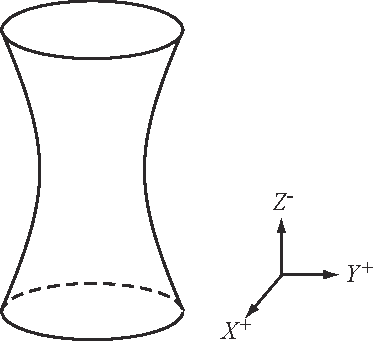
\includegraphics{Ch6_dS2.pdf} }
\vskip2mm
\caption{The embedding of dS$_2$ into $\mathbb{R}^{1,2}$. The figure looks the same as \fig{AdS2}, but the signature of the ambient spacetime differs from \fig{AdS2}.}
%dS$_2$ ����� $\mathbb{R}^{1,2}$ �ւ̖��ߍ��݁D\fig{AdS2}�Ƃقړ����ł��邪�C�e���ߍ��ݍ��W�̕���%���Ⴄ���Ƃɒ��ӁD}
\label{fig:dS2}
\end{figure}%
%%============

The \keyword{de~Sitter spacetime} is another spacetime with constant curvature, but this time constant positive curvature. It does not frequently appear in AdS/CFT, but the spacetime itself has been widely discussed in connection with the dark energy in cosmology. The two-dimensional de~Sitter spacetime, or the dS$_2$ spacetime is defined by
%�‚��łɁC������‚̒�ȗ�����Ƃ���{\bf �h�E�W�b�^�[����}\index{�Ƃ��‚��[������@�h�E�W�b�^�[����}������D�h�E�W�b�^�[����͐��̒�ȗ�������������ŁCAdS/CFT�œo�ꂷ��킯�ł͂Ȃ����C�ߔN�_�[�N�E�G�l���M�[�Ƃ̊֘A�ʼnF���_�I�ȋ����Ő���ɋc�_����Ă���D2�����h�E�W�b�^�[����idS$_2$�j�́C�ȉ��̂悤�ɒ�`�����i\fig{dS2}�j�F
\begin{gather}
%
ds^2 = - dZ^2 + dX^2 + dY^2~,
\label{eq:embed_ds2} \\
-Z^2 + X^2 + Y^2 = + L^2~,
\label{eq:surface_ds2}
%
\end{gather}
(\fig{dS2}). The dS$_2$ spacetime has the $SO(1,2)$ invariance. In the coordinates 
%dS$_2$�����$SO(1,2)$�Ώ̐������D
\be
%
X = L \cosh\tg \cos\theta~, \quad Y = L \cosh\tg \sin\theta~, \quad Z = L \sinh\tg~,
%
\ee
the metric becomes %�Ƃ������W�n���Ƃ�ƁC
\be
%
ds^2 = L^2 (- d\tg^2 + \cosh^2\tg\, d\theta^2)~.
\label{eq:metric_ds2}
%
\ee
The dS$_2$ spacetime has a constant positive curvature $R=2/L^2$. One often considers the AdS$_5$ spacetime for applications to AdS/CFT, but for the dS spacetime, one often considers the dS$_4$ spacetime for applications to cosmology.
%AdS����̏ꍇ�CAdS$_5$ ������l���邱�Ƃ��������CdS ����̏ꍇ�͉F���_�I�ȋ������� dS$_4$���� ���l���邱�Ƃ������D

%%------------------
\subsection{Relation with constant curvature spaces}
%��ȗ���ԂƂ̊֌W}%\label{sec:}
%%------------------

We saw various spaces and spacetimes, but the spacetimes with constant curvature are related to the spaces with constant curvature. Take a constant curvature spacetime. The Euclidean rotation of the timelike direction gives a constant curvature space:
%���܂��܂ȋ�ԁE���󂪓o�ꂵ�����C��ȗ�����͒�ȗ���ԂƊ֌W������D��ȗ���������[�N���b�h���������̂��C��ȗ���Ԃł���F
\be
%
\boxeq{
\begin{aligned}
\text{AdS}_2 &\xrightarrow{\text{Euclidean}}{} \text{H}^2 \\
\text{dS}_2 &\xrightarrow{\text{Euclidean}}{} S^2
\end{aligned}
}
%
\ee
The dS$_2$ spacetime and $S^2$ are defined by
%dS$_2$ ����� $S^2$ �́C
\begin{align}
%
\text{dS}_2: &&  ds^2 &= - dZ^2 \!+\! dX^2 \!+\! dY^2~, & -Z^2 \!+\! X^2 \!+\! Y^2 &= L^2~.
\\
S^2: && ds^2 &= dZ^2 \!+\! dX^2 \!+\! dY^2~, & Z^2 \!+\! X^2 \!+\! Y^2 &= L^2~.
%
\end{align}
The dS$_2$ spacetime becomes $S^2$ by $Z_\text{E} = iZ$. The AdS$_2$ spacetime and $H^2$ are defined by
%�ŗ^������̂ŁCdS$_2$ ����� $Z_\text{E} = iZ$ �Ƃ���ƁC$S^2$ �Ƀ��[�N���b�h�������DAdS$_2$ ����� H$^2$ �́C
\begin{align}
%
\text{AdS}_2: && ds^2 &= -dZ^2 \!-\! dX^2 \!+\! dY^2~, & -Z^2 \!-\! X^2 \!+\! Y^2 &= -L^2~.
\\
H^2: && ds^2 &= - dZ^2 \!+\! dX^2 \!+\! dY^2~, & -Z^2 \!+\! X^2 \!+\! Y^2 &= -L^2~.
%
\end{align}
%We permuted the coordinates $(X,Y,Z)$ for AdS$_2$ from the ones used previously. 
The AdS$_2$ spacetime becomes $H^2$ by $X_\text{E} = iX$. The Euclidean spacetime is often used in AdS/CFT.
%�ŗ^������̂Łi���Ղ����邽�߂�AdS$_2$����̏��������������j�CAdS$_2$ ����� $X_\text{E} = iX$ �Ƃ���ƁCH$^2$ �Ƀ��[�N���b�h�������DAdS/CFT�ł̓��[�N���b�h������������C���΂��Ηp������D


%%------------------
\subsection{Various coordinate systems of AdS spacetime
%AdS����̂��܂��܂ȍ��W�n
}\label{sec:AdS_coordinates}
%%------------------

So far we discussed the AdS spacetime using the global coordinates $(\tg, \rho)$:
%����܂�AdS�����
\be
%
\frac{ds^2}{L^2} = - \cosh^2\rho\, d\tg^2 + d\rho^2~.
%
\ee
But various other coordinate systems appear in the literature.
%�Ƃ����O���[�o�����W $(\tg, \rho)$ ���g���ċc�_���Ă������C�ق��ɂ������‚��̍��W�n�����΂��Γo�ꂷ��D

%%------------------
\subsubsection*{Static coordinates
%�ÓI���W 
$(\tg, \rs)$}%\label{sec:}
\index{static coordinates}
%\index{�����Ă����Ђ悤@�ÓI���W}
%%------------------

The coordinate $\rs$ is defined by $\rs := \sinh\rho$. The metric becomes
%$\rs := \sinh\rho$ �ƒ�`����C
\be
%
\frac{ds^2}{L^2} = - (\rs^2+1)\, d\tg^2 + \frac{d\rs^2}{\rs^2+1}~.
\label{eq:ads2_static}
%
\ee
This coordinate system is useful to compare with the AdS black hole (\sect{spherical_SAdS}).
% ���̍��W�n�́C�u���b�N�z�[��������ꍇ�Ƃ̊֌W�����₷���i\sect{spherical_SAdS}�j�D

%%------------------
\subsubsection*{Conformal coordinates
%�R���t�H�[�}�����W 
$(\tg, \theta)$}%\label{sec:}
\index{conformal coordinates}
%\index{����ӂ��[�܂邳�Ђ悤@�R���t�H�[�}�����W}
%%------------------

The coordinate $\theta$ is defined by $\tan \theta := \sinh\rho$ ($\theta: -\pi/2 \rightarrow \pi/2$).
The metric becomes flat up to an overfall factor (conformally flat)\index{conformally flat}%
\footnote{The name ``conformal coordinates" is not a standard one.}:
%$\tan \theta := \sinh\rho$ �ƒ�`����%
%\footnote{�u�R���t�H�[�}�����W�v�Ƃ����Ăѕ��͕W���I�Ƃ����킯�ł͂Ȃ��D}
%�i$\theta: -\pi/2 \rightarrow \pi/2$�j�C
\be
%
\frac{ds^2}{L^2} = \frac{1}{\cos^2\theta} (- d\tg^2 + d\theta^2 )~.
\label{eq:ads2_conf}
%
\ee
The AdS spacetime is represented as \fig{AdS2_Penrose} in this coordinate system. What is important is the existence of the spatial ``boundary" at $\theta=\pm\pi/2$. This boundary is called the \keyword{AdS boundary}. The AdS boundary is located at $\rs\rightarrow\infty$ in static coordinates and is located at $\rP\rightarrow\infty$ in \poincare\ coordinates below. The existence of the boundary means that one should specify the boundary condition on the AdS boundary in order to solve initial-value problems. From the AdS/CFT point of view, this boundary condition corresponds to specifying external sources one adds in the gauge theory side (\chap{GKPW}).
%���������āC���̍��W�n�ł�AdS�����\fig{AdS2_Penrose} �̂悤�ɂȂ�D�����ŁC$\theta=\pm\pi/2$ �Ɏ��ԓI�ɐL�т�u���E�v������_���d�v�ł���D���̋��E��{\bf AdS���E}\index{AdS���悤����@AdS���E}�ƌĂԁD�ÓI���W�ł�$r\rightarrow\infty$�C�ȉ��̃|�A���J�����W�ł�$\rP\rightarrow\infty$��AdS���E�ł���D���̂��Ƃ́C�����l���������ɂ́CAdS���E�ł̋��E�������w�肷��K�v�����邱�Ƃ��Ӗ�����DAdS/CFT�̗���ł́C���̋��E�����̓Q�[�W���_�ɉ�����O����w�肷�邱�Ƃɑ�������i\chap{GKPW}�j�D

%%============
\begin{figure}[tb]
\centering
%\hspace{0.25in}
\scalebox{0.75}{ 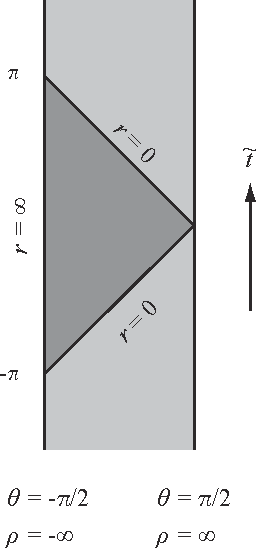
\includegraphics{Ch6_AdS2_Penrose.pdf} }
\vskip2mm
\caption{The AdS$_2$ spacetime in conformal coordinates. The \poincare\ coordinates cover only part of the full AdS spacetime which is shown in the dark shaded region (\poincare\ patch).}
%�R���t�H�[�}�����W�ł�AdS$_2$����D}
\label{fig:AdS2_Penrose}
\end{figure}%
%%============

%%------------------
\subsubsection*{\poincare\ coordinates 
%�|�A���J�����W
$(t, \rP)$}%\label{sec:}
\index{Poincar\'{e} coordinates}
%\index{�ق��񂩂ꂳ�Ђ悤@�|�A���J�����W}
%%------------------

This coordinate system is defined by
%���̍��W�n�́i$\rP>0$, $t:-\infty\rightarrow\infty$�j�C
% corrected
%\begin{subequations}
%\label{eq:}
\begin{align}
%
Z &= \frac{L\rP}{2} \left( -t^2 + \frac{1}{\rP^2} + 1 \right)~, \\
X &= L \,\rP\, t~, \\
Y &= \frac{L\rP}{2} \left( -t^2 + \frac{1}{\rP^2} - 1 \right)~, 
%X &= L \,\rP\, t~, \\
%Y &= \frac{L}{2\rP} \left\{ 1+ \rP^2(1 - t^2) \right\}~, \\
%Z &= \frac{L}{2\rP} \left\{ 1- \rP^2(1 + t^2) \right\}~, 
%\label{eq:}
%
\end{align}
%\end{subequations}
($\rP>0$, $t:-\infty\rightarrow\infty$). The metric becomes
%�Œ�`����C�v�ʂ�
\be
%
\boxeq{
\frac{ds^2}{L^2} = - \rP^2 dt^2 + \frac{d\rP^2}{\rP^2}~.
}
\label{eq:ads2_poincare}
%
\ee
This is the most often used coordinate system in AdS/CFT. This coordinate system is also useful to compare with the AdS black hole (\sect{SAdS}).
%���̍��W�n���C�u���b�N�z�[��������ꍇ�Ƃ̊֌W�����₷���i\sect{SAdS}�j�D


%%------------------
\subsection{Higher-dimensional cases
%��ʂ̎����̏ꍇ
}\label{sec:higher_AdS}
%%------------------

The spaces/spacetimes with constant curvature discussed so far can be easily generalized to the higher-dimensional case. In all examples, adding $p$ spatial directions to ambient spacetimes gives the $(p+2)$-dimensional cases.
%����܂ŋc�_������ȗ���ԁ^����́C��ԕ�����$p$�V���ɂ‚������邱�ƂŁC��ʂ�$(p+2)$��������ɗe�ՂɊg�����邱�Ƃ��ł���D

%%------------------
\subsubsection*{The sphere $S^{p+2}$}%\label{sec:}
%%------------------

The unit $S^{p+2}$ has the $SO(p+3)$ invariance and is defined by
\begin{gather}
%
ds_{p+3}^2 = d\omega_1^2 + \cdots + d\omega_{p+3}^2~, \\
\omega_1^2 + \cdots + \omega_{p+3}^2 = + 1~.
%
\end{gather}
The $S^{p+2}$ symmetry contains the $SO(p+2)$ invariance as a subgroup, which can be used to write the metric. For example, the unit $S^3$ coordinates can be chosen using $S^2$ coordinates $(\theta_2, \theta_3)$ as 
\be
%
\omega_2 = r \cos\theta_2~, \quad 
\omega_3 = r \sin\theta_2 \cos\theta_3~, \quad
\omega_4 = r \sin\theta_2 \sin\theta_3~,
%\label{eq:}
%
\ee
and $\omega_1^2=1-r^2$. Then,
\be
%
ds^2 = d\omega_1^2 + dr^2 + r^2 d\Omega_2^2 
= \frac{dr^2}{1-r^2} + r^2 d\Omega_2^2~,
%\label{eq:}
%
\ee
where $d\Omega_2^2 = d\theta_2^2 + \sin^2\theta_2\,d\theta_3^2$.
In the coordinate $r^2 = \sin^2\theta_1$ $(0 \leq \theta_1 <\pi)$, 
\be
%
d\Omega_3^2 = d\theta_1^2 + \sin^2\theta_1 d\Omega_2^2~.
%\label{eq:}
%
\ee
The similar construction can be done for $S^n$. So, one can construct the $S^n$ metric iteratively:
\begin{align}
%
d\Omega_n^2 
&= d\theta_1^2 + \sin^2\theta_1 d\Omega_{n-1}^2 \\
&= d\theta_1^2 
+ \sin^2\theta_1 d\theta_2^2 
+ \cdots 
+ \sin^2\theta_1 \cdots \sin^2\theta_{n-1} d\theta_n^2~,
%\label{eq:}
%
\end{align}
where $0 \leq \theta_i <\pi$ $(1 \leq i \leq n-1)$ and $0 \leq \theta_n <2\pi$.

%%------------------
\subsubsection*{The hyperbolic space $H^{p+2}$}%\label{sec:}
%%------------------

$H^{p+2}$ has the $SO(1,p+2)$ invariance and is defined by
%H$^{p+2}$ �� $SO(1,p+2)$ �Ώ̐��������C
\begin{gather}
%
ds_{p+3}^2 = - dX_0^2 + dX_1^2 + \cdots + dX_{p+2}^2~, \\
-X_0^2 + X_1^2 + \cdots + X_{p+2}^2 = - L^2~.
%
\end{gather}
For $p=0$, we set $X_0=Z$, $X_1=X$, and $X_2=Y$. 
The $H^{p+2}$ symmetry contains the $SO(p+2)$ invariance as a subgroup, so one can utilize the unit $S^{p+1}$ coordinates $\omega_i$ $(i =1, \ldots, p+2)$ to write the $H^{p+2}$ metric:
%�Œ�`�����D
\begin{gather}
%
X_0 = L \cosh\rho, \quad X_i = L\sinh\rho\, \omega_i~. %\\ 
%\textstyle{(i = 1,\ldots, p+2, \sum_{i=1}^{p+2} \omega_i^2=1)}~, \nonumber
%
\end{gather}
Then, the metric becomes
%�Ƃ������W�n�ł�
\be
%
\frac{ds^2}{L^2} = d\rho^2 + \sinh^2\rho\, d\Omega_{p+1}^2~.
%
\ee

%%------------------
\subsubsection*{The AdS$_{p+2}$ spacetime%
%AdS$_{p+2}$����
}%\label{sec:}
%%------------------

The AdS$_{p+2}$ spacetime has the $SO(2,p+1)$ invariance and is defined by
%AdS$_{p+2}$ ����� $SO(2,p+1)$ �Ώ̐��������C
\begin{gather}
%
ds_{p+3}^2 = - dX_0^2 - dX_{p+2}^2 + dX_1^2 + \cdots + dX_{p+1}^2~, \\
-X_0^2 - X_{p+2}^2 + X_1^2+ \cdots + X_{p+1}^2 = - L^2~.
%
\end{gather}
For $p=0$, we set $X_0=Z$, $X_{p+2}=X$, and $X_{p+1}=Y$. 
Just like AdS$_2$, the AdS$_{p+2}$ spacetime becomes  $H^{p+2}$ by $X_\text{E} = iX_{p+2}$.
%�Œ�`�����DAdS$_2$ ����Ɠ��l�ɁC$X_\text{E} = iX_{p+2}$ �Ƃ���� H$^{p+2}$ �Ƀ��[�N���b�h�������D 

The AdS$_{p+2}$ symmetry contains the $SO(p+1)$ invariance as a subgroup, and one can utilize the unit $S^{p}$ coordinates $\omega_i$ $(i =1, \ldots, p+1)$ to write the AdS$_{p+2}$ metric:
%AdS$_{p+2}$ ����̃O���[�o�����W��
%\mathindent=0zw % <-- [1]
\begin{gather}
%
X_0 = L \cosh\rho \cos\tg~, \quad X_{p+2} = L \cosh\rho \sin\tg~, \quad
X_i = L \sinh\rho\, \omega_i~. %\\
%\textstyle{(i = 1,\ldots, p+1, \sum_{i=1}^{p+1} \omega_i^2=1)}~. \nonumber
%
\end{gather}
%\mathindent=2zw % <-- [2] �f�t�H���g
This is the global coordinates for AdS$_{p+2}$. The metric becomes
%�ŗ^�����C�v�ʂ�
\be
%
\frac{ds^2}{L^2} = - \cosh^2\rho\, d\tg^2 + d\rho^2 + \sinh^2\rho\, d\Omega_{p}^2~.
%
\ee
One can define the other coordinate systems just like AdS$_2$. In static coordinates where $\rs := \sinh\rho$, the metric becomes
%�O���[�o�����W�n�ȊO�̍��W�n���CAdS$_2$ ����Ɠ��l�ɂƂ邱�Ƃ��ł���D�ÓI���W�ł�
\be
%
\frac{ds^2}{L^2} = - (\rs^2+1)\, d\tg^2 + \frac{d\rs^2}{\rs^2+1} + \rs^2 d\Omega_{p}^2~.
%
\ee
In conformal coordinates where $\tan \theta := \sinh\rho$, the metric becomes
%�R���t�H�[�}�����W�ł�
\be
%
\frac{ds^2}{L^2} = \frac{1}{\cos^2\theta} (- d\tg^2 + d\theta^2 + \sin^2\theta\, d\Omega_{p}^2)~.
%
\ee
For AdS$_{p+2}$, the \poincare\ coordinates are defined by
%�|�A���J�����W�́CAdS$_{p+2}$ ����̏ꍇ
%corrected
%\begin{subequations}
%\label{eq:}
\begin{align}
%
X_0 &= \frac{L\rP}{2} \left( x_i^2 - t^2 + \frac{1}{\rP^2} + 1 \right)~, \\
X_{p+2} &= L \,\rP\, t~, \\
X_i &= L\, \rP\, x_i \quad (i = 1,\ldots, p)~, \\
X_{p+1} &= \frac{L\rP}{2} \left( x_i^2 - t^2 + \frac{1}{\rP^2} - 1 \right)~.
%X_0 &= L \,\rP\, t~, \\
%X_i &= L\, \rP\, x_i \quad (i = 1,\ldots, p)~, \\
%X_{p+1} &= \frac{L}{2\rP} \left\{ 1- \rP^2(1 - x_i^2 + t^2) \right\}~, \\
%X_{p+2} &= \frac{L}{2\rP} \left\{ 1+ \rP^2(1 + x_i^2 - t^2) \right\}~.
%\label{eq:}
%
\end{align}
%\end{subequations}
The metric becomes
%�Œ�`����C
\be
%
\boxeq{
\frac{ds^2}{L^2} = \rP^2 (-dt^2+d\bmx_p^2) + \frac{d\rP^2}{\rP^2}~.
}
%
\ee
When $p=3$, the metric coincides with the near-horizon limit of the D3-brane \eqref{eq:D3_near_horizon}. 

%The AdS$_{p+2}$ spacetime is a solution of the Einstein equation with a negative cosmological constant $\Lambda=-p(p+1)/(2L^2)$:
%AdS$_{p+2}$ ����͕��̉F���萔 $\Lambda=-p(p+1)/(2L^2)$ �����ƒA�C���V���^�C���������̉��ł���F
%\be
%
%R_{MN} - \frac{1}{2} g_{MN} R + \Lambda g_{MN} = 0~.
%\label{eq:Einstein_cc}
%
%\ee
% added
%You can compute curvature tensors explicitly to show that the AdS$_{p+2}$ spacetime is a solution of the Einstein equation with a negative cosmological constant:
%\be
%
%R_{MN} - \frac{1}{2} g_{MN} R + \Lambda g_{MN} = 0~.
%\label{eq:Einstein_cc}
%
%\ee
%But a spacetime with constant curvature is always a solution of the Einstein equation as below. The constant curvature implies that the Ricci tensor is proportional to the metric:
%\be
%
%R_{MN} = \frac{R}{p+2}\, g_{MN}
%\label{eq:}
%
%\ee
%with a constant $R$. Then, it always satisfies the Einstein equation with an appropriately chosen $\Lambda$:
%\be
%
%R_{MN} - \frac{1}{2} g_{MN} R = -\frac{p}{2(p+2)} R\, g_{MN}~.
%\label{eq:}
%
%\ee
%The explicit computation of the Ricci scalar shows $R=-(p+1)(p+2)/L^2$, so $\Lambda=-p(p+1)/(2L^2)$.

%%------------------
\subsubsection*{The dS$_{p+2}$ spacetime
%dS$_{p+2}$����
}%\label{sec:}
%%------------------

The dS$_{p+2}$ spacetime has the $SO(1,p+2)$ invariance and is defined by
%dS$_{p+2}$ ����� $SO(1,p+2)$ �Ώ̐��������C
\begin{gather}
%
ds_{p+3}^2 = - dX_0^2 + dX_1^2 + \cdots + dX_{p+2}^2~, \\
- X_0^2 + X_1^2 + \cdots + X_{p+2}^2 = + L^2~.
%
\end{gather}
For $p=0$, we set $X_0=Z$, $X_1=X$, and $X_2=Y$. 
Just like dS$_2$, the dS$_{p+2}$ spacetime becomes $S^{p+2}$ by $X_\text{E} = iX_0$. 

The dS$_{p+2}$ symmetry contains the $SO(p+2)$ invariance as a subgroup, and one can utilize the unit $S^{p+1}$ coordinates $\omega_i$ $(i =1, \ldots, p+2)$ to write the dS$_{p+2}$ metric:
%�Œ�`�����DdS$_2$ ����Ɠ��l�ɁC$X_\text{E} = iX_0$ �Ƃ���� $S^{p+2}$ �Ƀ��[�N���b�h�������D 
% 2014/1/9: corrected
\begin{gather}
%
X_0 = L \sinh\tg, \quad X_i = L \cosh\tg\, \omega_i~. %\\
%\textstyle{(i = 1,\ldots, p+2, \sum_{i=1}^{p+2} \omega_i^2=1)}~, \nonumber
%
\end{gather}
Then, the metric becomes
%�Ƃ������W�n�ł�
\be
%
\frac{ds^2}{L^2} = - d\tg^2 + \cosh^2\tg\, d\Omega_{p+1}^2~.
%
\ee
%The dS$_{p+2}$ spacetime is a solution of the Einstein equation \eqref{eq:Einstein_cc} with a positive cosmological constant $\Lambda=p(p+1)/(2L^2)$.
%dS$_{p+2}$ ����͐��̉F���萔 $\Lambda=p(p+1)/(2L^2)$ �����ƒA�C���V���^�C�������� \eqref{eq:Einstein_cc} �̉��ł���D

% added
%%------------------
\subsubsection*{Maximally symmetric spacetimes}%\label{sec:}
%%------------------

We saw that these spacetimes have a large number of symmetries like $S^2$. In fact, they are called \keyword{maximally symmetric spacetimes} which admit the maximum number of symmetry generators. As a familiar example, the Minkowski spacetime is also a spacetime with constant curvature (namely $R=0$) and is a maximally symmetric space. The $(p+2)$-dimensional Minkowski spacetime has the $ISO(1,p+1)$ \poincare\ invariance. The number of symmetry generators is $(p+1)(p+2)/2$ for $SO(1,p+1)$ and $(p+2)$ for translations, so $(p+2)(p+3)/2$ in total. 
%The number of symmetry generators is
%\be
%\begin{split}
%
%SO(1,p+1): & \frac{1}{2}(p+1)(p+2) \\
%\text{translations:} & p+2
%
%\end{split}
%\ee
%\be
%
%\left.
%\begin{array}{ll}
%SO(1,p+1): & \frac{1}{2}(p+1)(p+2) \\
%\text{translations:} & p+2
%\end{array}
%\right\} 
%= \frac{1}{2}(p+2)(p+3)~.
%\label{eq:}
%
%\ee
%\be
%
%\frac{1}{2}(p+2)(p+3)=
%\left\{
%\begin{array}{ll}
%\frac{1}{2}(p+1)(p+2)& \text{for } SO(1,p+1) \\
%p+2 &\text{for translations} 
%\end{array}
%\right.
%\label{eq:}
%
%\ee
This is the maximum number of generators. Figure~\ref{fig:sym} summarizes the symmetries of spaces/spacetimes with constant curvature. They all have the same maximum number of generators.

As a consequence of a maximally symmetric spacetime, it is known that the Riemann tensor is written as 
\be
%
R_{ABCD} = \pm \frac{1}{L^2} (g_{AC}g_{BD} - g_{AD}g_{BC})
%\label{eq:}
%
\ee
($+$ for positive curvature and $-$ for negative curvature). Then, the Ricci tensor and the Ricci scalar are 
\be
%
R_{MN} = \pm \frac{p+1}{L^2} g_{MN}~, \quad
R = \pm \frac{(p+1)(p+2)}{L^2}~.
%\label{eq:}
%
\ee
When $p=0$, we recover $R=\pm 2/L^2$. Then, a maximally symmetric spacetime is a solution of the Einstein equation with an appropriately chosen cosmological constant $\Lambda$:
\be
%
R_{MN} - \frac{1}{2} g_{MN} R = \mp \frac{p(p+1)}{2L^2} g_{MN}~,
\label{eq:Einstein_cc2}
%
\ee
which fixes $\Lambda=\pm p(p+1)/(2L^2)$.

% added
%%============
\begin{figure}[tb]
\begin{center}
\begin{tabular}{|c|c||c|c|}
%
\hline
Space & Symmetry & Spacetime & Symmetry \\
\hline
$S^{p+2}$	& $SO(p+3)$	& dS$_{p+2}$	& $SO(1,p+2)$ \\
$H^{p+2}$	& $SO(1,p+2)$	& AdS$_{p+2}$	& $SO(2,p+1)$ \\
\hline
%
\end{tabular}
\caption{Symmetries of spaces/spacetimes with constant curvature.}
\label{fig:sym}
\end{center}
\end{figure}
%%============

%%%%%%%%%
\section{Particle motion in AdS spacetime \advanced
%AdS����ł̗��q�̉^��
}\label{sec:geodesics_AdS}
%%%%%%%%%

Readers may skip this section in a first reading because the AdS physics is not intuitively very clear. %AdS����͂Ȃ��Ȃ������������ɂ����̂ŁC�ŏ��ɓǂނƂ��͂Ƃ΂��Ă������‚����Ȃ��D

%%------------------
\subsubsection*{Gravitational redshift
%�d�͐ԕ��Έ�
}%\label{sec:}
%%------------------

Let us consider the gravitational redshift in static coordinates $(\tg,\rs)$. \index{static coordinates}
%Recall the gravitational redshift formula \index{gravitational redshift} in \eq{red_shift}:
%\be
%
%\frac{E_B}{E_A} =\sqrt{\frac{g_{00}(A)}{g_{00}(B)}}~.
%\label{eq:red_shift}
%
%\ee
%We consider the redshift in static coordinates. \index{static coordinates} 
Consider two static observers, the observer A at the origin $\rs=0$ and the observer B at $\rs=\rs_B \gg 1$. The observer A sends a photon. From the redshift formula \eqref{eq:red_shift}, the photon energy received by B is given by
%�܂��C�ÓI���W\index{�����Ă����Ђ悤@�ÓI���W}��AdS����ł̏d�͐ԕ��Έ�\index{���䂤��悭�����ق��ւ�@�d�͐ԕ��Έ�}���l����D���_$r=0$�ɐÎ~�����ϑ���A�ƁC$r=r_B \gg 1$�ɐÎ~�����ϑ���B������Ƃ���D\eq{red_shift}���g���ƁCA�����������q�̃G�l���M�[��B�ɂƂ���
\be
%
\frac{E_B}{E_A} =\sqrt{\frac{g_{00}(A)}{g_{00}(B)}}
\result
E_B \simeq \left(\frac{1}{\rs_B}\right) E_A~.
\label{eq:red_shift_AdS}
%
\ee
Thus, the photon energy decreases at B. In particular, when $\rs_B\rightarrow\infty$, $E_B\rightarrow0$, so the photon gets an infinite redshift. The gravitational redshift comes from the gravitational potential, so this implies that $\rs=0$ is the ``bottom" of the gravitational potential well. The fact that the photon gets an infinite redshift is similar to a black hole, but the AdS spacetime is not a black hole.
%�ƂȂ�D���������āCB�ɂƂ��Č��q�̃G�l���M�[�͌�������D�Ƃ��� $r_B\rightarrow\infty$�̏ꍇ�C$E_B\rightarrow0$�Ȃ̂ŁC���q�͖����̐ԕ��Έڂ��󂯂�D�d�͐ԕ��Έڂ͏d�̓|�e���V�����ɂ����ʂȂ̂ŁC���̂��Ƃ�$r=0$���d�̓|�e���V�����́u��v�ɂ����邱�Ƃ��Ӗ�����D�Ȃ��C���q�������̐ԕ��Έڂ��󂯂�̂̓z���C�Y���Ǝ��Ă��邪�CAdS����̓u���b�N�z�[���ł͂Ȃ��D

%%------------------
\subsubsection*{Photon motion
%���q�̉^��
}%\label{sec:}
%%------------------

Let us examine the photon and particle motions in the AdS spacetime. Such analysis can be done just like the particle motion analysis in the Schwarzschild black hole (\sect{geodesics_horizon}), but the photon and the particle have strange behaviors in the AdS spacetime. Take the static coordinates and consider a particle which starts from the bottom of the gravitational potential $\rs=0$ to $\rs=\infty$. We set $L=1$ below for simplicity.
%AdS����ł̌��q�◱�q�̉^���𒲂ׂĂ݂悤�D���̂悤�ȉ�͂́C\sect{geodesics_horizon}�ł̃V�������c�V���h�E�u���b�N�z�[���ł̗��q�̉^���Ɠ��l�ɂ����Ȃ��邪�CAdS����ł͗��q�͊�ȐU��܂�������D���܁C�ÓI���W�ŏd�̓|�e���V�����̒�$r=0$����$r=\infty$�Ɍ������ĉ^�����闱�q���l����D�ȉ��C�ȒP�̂��߂�$L=1$�Ƃ���D

First, consider the photon motion $ds^2=0$ from the point of view of the coordinate time $\tg$. This is the simplest in conformal coordinates:
%�܂����q�̉^�����C���W����$\tg$�̗���Œ��ׂ�D����̓R���t�H�[�}�����W���g���ƊȒP�ŁC
\be
%
ds^2 = \frac{1}{\cos^2\theta} (- d\tg^2 + d\theta^2 ) = 0
\result 
\frac{d\theta}{d\tg} = 1~.
%\label{eq:}
%
\ee
Since $\rs=\tan\theta$, $\rs:0\rightarrow\infty$ corresponds to $\theta:0\rightarrow\pi/2$, and
%$r=\tan\theta$�Ȃ̂ŁC$r:0\rightarrow\infty$��$\theta:0\rightarrow\pi/2$�ɑ������C
\be
%
\tg = \int_0^{\pi/2} d\theta = \frac{\pi}{2}~.
%\label{eq:}
%
\ee
Namely, the photon reaches the AdS boundary in a \textit{finite} coordinate time. We thus need a boundary condition at the AdS boundary: how the photon behaves at the AdS boundary depends on the boundary condition at the AdS boundary (\eg, it reflects back to the origin).
%���Ȃ킿�C���W����$\tg$�ł͗L�����Ԃ�AdS���E�ɓ��B����DAdS���E�ł̐U��܂��i���Ƃ��Ό��_�ɖ߂��Ă��邩�ǂ����j��AdS���E�ł̋��E��������ł���DAdS���E�ł̋��E�������K�v�Ȃ��Ƃ��킩��D

But consider the motion from the point of view of the ``proper time" $\tau$ (one cannot define the proper time for the photon, but one can define an affine parameter, so $\tau$ is an affine parameter\index{affine parameter}). From $p^2=0$, 
%����C�u�ŗL���ԁv�̗���$\tau$�ł́i���q�ɑ΂��Ă�$\tau$���ŗL���ԂƂ��ĉ��߂ł��Ȃ��̂ŁC�A�t�B���p�����[�^\index{���ӂ���͂�߁[��@�A�t�B���p�����[�^}�Ƃ����Ӗ��ł���j
\be
%
g^{00} E^2 + g_{\rs\rs} \left(\frac{d\rs}{d\tau}\right)^2 = 0~.
%
\ee
We define the energy $E$ for the photon as $p_0=:-E$. Then,
%���q�ɑ΂��Ă� $p_0=:-E$�Ƃ���$E$���`�����D
\be
%
- \frac{E^2}{\rs^2+1} + \frac{1}{\rs^2+1} \left( \frac{d\rs}{d\tau} \right)^2 = 0
\result
\frac{d\rs}{d\tau} = E~.
\label{eq:null_dtau}
%
\ee
Thus, $\rs=E\tau$, namely it takes an \textit{infinite} affine parameter time until the photon reaches the AdS boundary.
%���������āC$r=E\tau$�C�‚܂���q��AdS���E�ɓ��B����̂́C�A�t�B���p�����[�^�ł͖����́u���Ԍ�v�ł���D

%%------------------
\subsubsection*{Particle motion
%���q�̉^��
}%\label{sec:}
%%------------------

%%============
\begin{figure}[tb]
\centering
\scalebox{0.75}{ 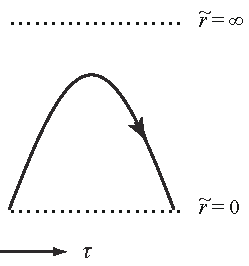
\includegraphics{Ch6_AdS_box.pdf} }
\caption{In the AdS spacetime, a particle cannot reach the boundary $\rs\rightarrow\infty$ and comes back to the origin in a finite proper time and coordinate time. }
\label{fig:potential_well} 
\end{figure}%
%%============

Now, consider the particle motion from the point of view of the proper time $\tau$. From $p^2=-m^2$, 
%���q�̏ꍇ�C�܂��ŗL����$\tau$�̗���ł́C
\begin{align}
%
g^{00} E^2 + g_{\rs\rs} \left(\frac{d\rs}{d\tau}\right)^2 = -1 
&\result
- \frac{E^2}{\rs^2+1} + \frac{1}{\rs^2+1} \left( \frac{d\rs}{d\tau} \right)^2 = -1 \\
%\label{eq:}
&\result
\left( \frac{d\rs}{d\tau} \right)^2 = (E^2-1) - \rs^2~.
\label{eq:timelike_dtau}
%\label{eq:}
%
\end{align}
Take $E>1$ so that the right-hand side of \eq{timelike_dtau} is positive at $\rs=0$. But the right-hand side becomes negative as $\rs\rightarrow\infty$, so the particle cannot reach the AdS boundary $\rs\rightarrow\infty$. This is the effect of the gravitational potential well in the AdS spacetime (\fig{potential_well}). The turning point $\rs_*$ is given by $\rs_* = \sqrt{E^2-1}$. Then,
%���_$r=0$��\eq{timelike_dtau}�̉E�ӂ����ł���悤�ɁC$E>1$�ƂƂ�D�������C$r\rightarrow\infty$�ʼnE�ӂ͕��ɂȂ��Ă��܂��̂ŁC���q��$r\rightarrow\infty$�ɓ��B�ł��Ȃ��DAdS����ɂ��|�e���V������ǂ̌��ʂł���D�]��_��$r_* = \sqrt{E^2-1}$�ŗ^������D
\be
%
\tau = \int_0^{\rs_*} \frac{ d\rs }{ \sqrt{(E^2\!-\!1) \!-\! \rs^2} }
= \int_0^{\pi/2} d\varphi 
= \frac{\pi}{2}~,
\label{eq:timelike_tau}
%
\ee
where $\rs =: \sqrt{E^2-1} \sin\varphi$.
%������ $r =: \sqrt{E^2-1} \sin\varphi$ �Ƃ����D

How about the motion in the coordinate time $\tg$? By definition $p^0 = md\tg/d\tau$, and from the conservation law, $p^0 = g^{00}p_0 = -mg^{00}E$. Thus,
%����C���W����$\tg$�̗���ł́C$p^0 = md\tg/d\tau$�C$p^0 = g^{00}p_0 = -mg^{00}E$ ���C
\be
%
\frac{d\tg}{d\tau} = \frac{E}{-g_{00}}~.
%\label{eq:}
%
\ee
Using \eq{timelike_tau}, one gets
%\eq{timelike_tau}���g���ƁC
%\mathindent=0zw % <-- [1]
\be
%
\tg = E \! \int_0^{\rs_*} \! \frac{ d\rs }{ (\rs^2\!+\!1)\sqrt{(E^2\!-\!1) \!-\! \rs^2} }
= E\! \int_0^{\pi/2} \! \frac{d\varphi }{ (E^2\!-\!1)\sin^2\varphi \!+\! 1 }
\!= \frac{\pi}{2}~.
%\label{eq:}
%
\ee
%\mathindent=2zw % <-- [2] �f�t�H���g
Namely, the particle returns to $\rs=0$ with the same amount of the coordinate time $\tg=\pi$ as the photon. The amount of time is the same in the particle proper time $\tau$. Also, the time for the particle to return does not depend on energy $E$. The particle goes further as you increase $E$, but it always returns with the same amount of time. These results are summarized in \fig{particle_motion}.
%�ȏ���C���q�͌��q���߂��Ă���̂Ɠ������W����$\tg=\pi$�Ŗ߂��Ă���D����͗��q�̌ŗL����$\tau$�ł������ł���D�܂��C���q���߂��Ă���܂ł̎��Ԃ́C�G�l���M�[$E$�ɂ��Ȃ��D$r_*$�̒�`���C$E$���傫���قǗ��q�͉����܂œ��B���邪�C�����鎞�Ԃ͓����ł���D

% added
%%============
\begin{figure}[tb]
\begin{center}
\begin{tabular}{|c||c|c|}
%
\hline
					& Photon & Particle \\
\hline
affine time $\tau$		& $\infty\ (\rs: 0\rightarrow\infty)$	& $\pi/2\ (\rs: 0\rightarrow \rs_*)$  \\
coordinate time $\tg$		& $\pi/2\ (\rs: 0\rightarrow\infty)$	& $\pi/2\ (\rs: 0\rightarrow \rs_*)$  \\
\hline
%
\end{tabular}
\caption{The affine time and the static coordinate time $\tg$ for the particle and the photon to reach the AdS boundary.}
\label{fig:particle_motion}
\end{center}
\end{figure}
%%============


%%------------------
\subsubsection*{\poincare\ coordinates and \poincare\ patch \index{Poincar\'{e} coordinates}
%�|�A���J�����W\index{�ق��񂩂ꂳ�Ђ悤@�|�A���J�����W}�ɂ‚���
}%\label{sec:}
%%------------------

We examined the motion using the static coordinate time $\tg$, but let us examine the same question using the \poincare\ coordinate time $t$. For simplicity, we consider only the photon motion. Consider the photon motion from $\rP=R$ to $\rP=0$. From  
%���W����$\tg$�̗��ꂾ���ł͂Ȃ��C�|�A���J�����W�̎���$t$�̗���ł����ׂĂ݂悤�D�ȒP�̂��߂Ɍ��q�̉^���������l����D���x�́C$\rP=R$����$\rP=0$�ւ̉^�����l���邱�Ƃɂ���D�܂��C���W����$t$�̗���ł́C
\be
%
ds^2 = -\rP^2dt^2 + \frac{d\rP^2}{\rP^2} = 0
\result 
\frac{d\rP}{dt} = -\rP^2~,
%\label{eq:}
%
\ee
one gets
%�Ȃ̂ŁC
\be
%
t = -\int_R^{\epsilon} \frac{ d\rP }{ \rP^2 }
= \left.\frac{1}{\rP} \right|_R^\epsilon 
= \frac{1}{\epsilon}-\frac{1}{R}
\rightarrow\infty~.
%\label{eq:}
%
\ee
Thus, it takes an infinite coordinate time $t$ until the photon reaches $\rP=0$.
%���������āC$\rP=0$�ɓ��B����ɂ͖����̍��W����$t$��������D

But this is not the case in the affine parameter $\tau$. Just like \eq{null_dtau}, 
%�������C�A�t�B���p�����[�^$\tau$�̗���ł͂����ł͂Ȃ��D\eq{null_dtau}�Ɠ��l�ɁC
\be
%
\frac{d\rP}{d\tau} = -E~,
%\label{eq:}
%
\ee
so it takes a finite affine time from $\rP=R$ to $\rP=0$%
\footnote{As in \eq{null_dtau}, it takes an infinite affine time from $\rP=\infty$ to $\rP=0$, but it takes a finite amount of time from finite $R$ to $\rP=0$.}.
%�Ȃ̂ŁC$\rP=R$����$\rP=0$�܂ł͗L���A�t�B���p�����[�^�œ��B����D

The behavior of the \poincare\ coordinates is similar to the Schwarzschild coordinates. Because the photon reaches $\rP=0$ in a finite affine parameter, the \poincare\ coordinates cover only part of the full AdS spacetime%
\footnote{Otherwise, the spacetime would be \keyword{geodesically incomplete} which signals a spacetime singularity. The geodesic incompleteness means that there is at least one geodesic which is inextensible in a finite ``proper time" (in a finite affine parameter). This is the definition of a spacetime singularity.}. 
From the point of view of the full AdS geometry, $t\rightarrow\infty$ as $\rP\rightarrow0$ because of the ill-behaved coordinates just like the Schwarzschild coordinates. The region covered by \poincare\ coordinates is called the \textit{\poincare\ patch} (\fig{AdS2_Penrose}).\index{Poincar\'{e} patch}
%�|�A���J�����W�̐U��܂��́C�V�������c�V���h���W�̐U��܂��Ǝ��Ă���D�܂��C$\rP=0$�܂ŗL���A�t�B���p�����[�^�œ��B����̂�����C�|�A���J�����W��AdS����̈ꕔ�����J�o�[���Ȃ����W�n�ł���D�|�A���J�����W�n���J�o�[����͈͂�{\bf �|�A���J���E�p�b�`}\index{�ق��񂩂�͂‚�@�|�A���J���E�p�b�`}�ƌĂԁDAdS����S�̗̂��ꂩ�猾���ƁC$\rP=0$��$t\rightarrow\infty$�ƂȂ�̂́C�V�������c�V���h���W���l�C���W�n�̖��ł���D

In this sense, the location $\rP=0$ is similar to the horizon but has a difference from the horizon. The region inside the horizon cannot influence the region outside. But the AdS spacetime does not have such a region. In conformal coordinates, clearly there is no region which cannot influence the AdS boundary. The \poincare\ patch is rather similar to the \keyword{Rindler spacetime}:
%�����̈Ӗ��ŁC$\rP=0$�̓z���C�Y���Ǝ��Ă��邪�C�V�������c�V���h�E�u���b�N�z�[���̃z���C�Y���Ƃ͂�␫�i���قȂ�D�R���t�H�[�}�����W�ł́CAdS���E�ɉe�����y�ڂ��Ȃ��̈�͂Ȃ�����ł���i\fig{AdS2_Penrose}�j�D�|�A���J�����W�́C�ނ���{\bf �����h���[����}\index{���Ƃ�[������@�����h���[����}�ƌĂ΂�鎞��Ɏ��Ă���F
\be
%
ds_{p+2}^2 = -r\, dt^2 + \frac{dr^2}{r} + d\bmx_p^2~.
\label{eq:rindler}
%
\ee
The Rindler spacetime is just the Minkowski spacetime although it does not look so (\probset{rindler}). The difference is that the Rindler spacetime covers only part of the Minkowski spacetime. Physically, the Rindler coordinates represent the observer who experiences a constant acceleration and there is a horizon, $r=0$, for the observer. But the horizon is observer-dependent, and the Minkowski spacetime as a whole has no horizon.
%�����h���[����͈ꌩ����Ƃ����݂͂��Ȃ���������Ȃ����C�~���R�t�X�L�[���󂻂̂��̂ł���C�������~���R�t�X�L�[����̈ꕔ�����J�o�[���Ă��Ȃ����W�n�ł���D�����I�ɂ́C�����x���̊ϑ��҂ɂƂ��Ă̍��W�n�ł���C���̊ϑ��҂ɂƂ��Ẵz���C�Y��������i$r=0$�j�D�������C�~���R�t�X�L�[����S�̂Ƃ��Ă݂��ꍇ�C�z���C�Y��������킯�ł͂Ȃ��D

Similarly, there is a horizon at $\rP=0$ for the observer inside the \poincare\ patch, but the AdS spacetime as a whole has no horizon. Whether $\rP=0$ is a horizon or not depends on the point of view%
\footnote{For example, in the near-horizon limit, the extreme RN-AdS$_4$ \bh becomes the AdS$_2$ spacetime in \poincare\ coordinates (\sect{others_HSC}). In this case, $\rP=0$ corresponds to the true horizon of the black hole. So, whether $\rP=0$ is a true horizon or not depends on the context.}. 
% omitted from Springer edition
%This $\rP=0$ horizon also appeared in the extreme RN black hole. The near-horizon limit of the extreme RN black hole becomes the AdS$_2$ spacetime in \poincare\ coordinates (\sect{RN}). In this case, $\rP=0$ corresponds to the true horizon of the RN black hole. So, again, whether $\rP=0$ is a horizon or not depends on the context. 
As a finial remark, the Rindler spacetime has a Hawking temperature,
%[one can compute the temperature using \eq{Hawking_temp}], 
but the AdS spacetime in \poincare\ coordinates has zero temperature. The Rindler spacetime has the following thermodynamic quantities:
\be
%
T = \frac{1}{4\pi}~, \quad
s = \frac{1}{4G}~, \quad
\varepsilon = 0~, \quad
P= \frac{1}{16\pi G}~.
%\label{eq:}
%
\ee
%���l�ɁC$\rP=0$�̓|�A���J���E�p�b�`���̊ϑ��҂ɂƂ��Ă̓z���C�Y�������CAdS����S�̂ł݂��ꍇ�C�z���C�Y��������킯�ł͂Ȃ��D�‚܂�C$\rP=0$���z���C�Y�����ǂ����́C����̖��ł���D�ʂ̗�Ƃ��āC�Ɍ�RN�u���b�N�z�[����near-horizon�Ɍ����Ƃ�ƁC�|�A���J�����W�ł�AdS$_2$���󂪂������i\sect{RN}�j�D���̏ꍇ��$\rP=0$�́C���ۂ�RN�u���b�N�z�[���̃z���C�Y���ɂ�����D�Ȃ��C�����h���[����͗L�����x�����‚��C�|�A���J�����W��AdS����͉��x�[���ł���D


%%%%%%%%%
\section{Remarks on AdS/CFT interpretations
%AdS/CFT�ł̉��߂ɂ‚���
}\label{sec:interpretation}
%%%%%%%%%

%%------------------
\subsubsection*{The symmetries of the AdS spacetime
%AdS����̑Ώ̐��ɂ‚���
}%\label{sec:}
%%------------------

Let us rewrite the AdS$_5$ spacetime in \poincare\ coordinates%
\footnote{So far we took dimensionless coordinates, but we take dimensionful ones below. }:
%We write the radial coordinate as $r$; this corresponds to $\rP$ and should not be confused with the $r$-coordinate in static coordinates. }
%�|�A���J�����W�ł� AdS$_5$ ��������炽�߂ď�����%
%\footnote{����܂ō��W�͖������ʂł���悤�ɂƂ��Ă������C�ȉ��ł͎��������‚悤�ɂƂ�D�܂��C���a���W�����炽�߂� $r$ �Ə������Ƃɂ��邪�C�ÓI���W�� $r$ �ł͂Ȃ��C�|�A���J�����W�� $\rP$ �ɑ�������D}�C
\be
%
ds_5^2 = \left( \frac{r}{L} \right)^2 (-dt^2+dx^2+dy^2+dz^2) 
+ L^2\frac{dr^2}{r^2}~.
\label{eq:ads_poincare}
%
\ee
The spacetime has the $SO(2,4)$ invariance, part of which can be seen easily in \poincare\ coordinates and are physically important:
%���̎���� $SO(2,4)$ �Ώ̐������‚��C�Ώ̐��̈ꕔ�̓|�A���J�����W�ŗe�Ղɓǂ݂Ƃ�C�܂������I�ɂ��d�v�ł���F
\begin{enumerate}
\item
\textit{Four-dimensional \poincare\ invariance}: The metric has the \poincare\ invariance $ISO(1,3)$ on $x^\mu=(t,x,y,z)$. This corresponds to the \poincare\ invariance of the dual gauge theory in four-dimensional spacetime, so $x^\mu$ is interpreted as the spacetime coordinates of the gauge theory. Similarly, for the AdS$_{p+2}$ spacetime, $p$ represents the number of the spatial dimensions of the dual gauge theory.
%{\bf �|�A���J���Ώ̐�}�F�v�ʂ� $x^\mu=(t,x,y,z)$ �ɑ΂��� $ISO(1,3)$ �|�A���J���Ώ̐������D���ꂪ4��������̃Q�[�W���_�̃|�A���J���Ώ̐��ɑ������C���������� $x^\mu$ ���Q�[�W���_�̍��W�Ɖ��߂���D���l�ɁC��ʂ� AdS$_{p+2}$ ����̏ꍇ�C$p$ �̓Q�[�W���_�̋�Ԏ���������킵�Ă���D
\item
\textit{Four-dimensional scale invariance}: The metric is invariant under
%{\bf �X�P�[���Ώ̐�}�F�v�ʂ́C
\be
%
\boxeq{
x^\mu \rightarrow a x^\mu, \quad r \rightarrow \frac{1}{a}\, r~.
}
\label{eq:scale_inv}
%
\ee
%�Ƃ����ϊ��̉��ŕs�ςł���D
\end{enumerate}

Under the scaling, $r$ transforms as energy which is conjugate to $t$. This is one reason why the gauge theory is four-dimensional whereas the gravitational theory is five-dimensional. Namely, the $r$-coordinate has the interpretation as the gauge theory energy scale. The ${\cal N}=4$ SYM has the scale invariance, but the invariance is realized geometrically in the dual gravitational theory.
%�X�P�[�����O \eqref{eq:scale_inv} �̉��ŁC$r$ ��$t$�ɋ����ȃG�l���M�[�Ɠ����ϊ��������D�Q�[�W���_�̎���4�����ŁC�d�͗��_�̎���5�����Ȃ̂́C���ꂪ1�‚̗��R�ł���D�‚܂�C$r$���W�̓Q�[�W���_�̃G�l���M�[�X�P�[���Ƃ����Ӗ������D${\cal N}=4$�Q�[�W���_���X�P�[���Ώ̐������‚��C�d�͗��_�ł͂�����􉽓I�Ɏ������Ă���̂ł���D

Let us examine more about the dual gauge theory energy. In AdS/CFT, the gauge theory time corresponds to the coordinate $t$ not to the proper time $\tau$. The proper time $\tau_r$ for the static observer at $r$ is related to the coordinate $t$ as
%�Q�[�W���_�̗���ł̃G�l���M�[�������������ׂĂ݂悤�DAdS/CFT�̏ꍇ�C�Q�[�W���_�̎��Ԃɑ�������͍̂��W$t$�ł���ŗL����$\tau$�ł͂Ȃ��D�ʒu$r$�ɐÎ~�����ϑ��҂ɂƂ��Ă̌ŗL����$\tau_r$�ƍ��W$t$�̂������ɂ́C
\be
%
d\tau_r^2 = |g_{00}(r)| dt^2~.
\label{eq:tau_vs_t}
%
\ee
Then, the proper energy for the observer at $r$, $E(r)$, is related to the gauge theory energy, $E_t$,  as%
\footnote{This equation looks similar to the gravitational redshift \eqref{eq:red_shift_AdS}, but the interpretations are different. The gravitational redshift compares proper energies at different radial positions. The UV/IR relation compares the proper energy and the energy conjugate to the coordinate $t$ at one radial position. }
%�̊֌W������̂ŁC$r$�̊ϑ��҂ɂƂ��Ă̌ŗL�G�l���M�[$E(r)$�ƃQ�[�W���_�̃G�l���M�[$E_t$�̊֌W��
\be
%
E_t =\sqrt{|g_{00}(r)|} E(r)
\simeq  \left(\frac{r}{L}\right) E(r)~.
\label{eq:UV/IR}
%
\ee
Consider an excitation in the AdS spacetime with a given proper energy (for example, a string). The gauge theory energy depends on where the excitation is located. The gauge theory energy is larger if the excitation is nearer the AdS boundary. The relation \eqref{eq:UV/IR} is called the \keyword{UV/IR relation}.
%�ƂȂ�%
%\footnote{���̎��́C�d�͐ԕ��Έڂ�\eq{red_shift_AdS}�ƕ\�ʏ㓯�������C�����߂��Ⴄ���Ƃɒ��ӁD�d�͐ԕ��Έڂ͓��a���W�̈Ⴄ�ꏊ�ł̌ŗL�G�l���M�[�ǂ������ׂĂ��邪�CUV/IR�֌W���͂��铮�a���W�ł̌ŗL�G�l���M�[�ƍ��W$t$�ɋ����ȃG�l���M�[���ׂĂ���D}�D
%�ŗL�G�l���M�[$E(r)$�������ł����Ă��C���a�����̈ʒu$r$����ŁC�Q�[�W���_�Ƃ��ẴG�l���M�[�͈قȂ�DAdS���E�ɋ߂Â��ɂ‚�āC�Q�[�W���_�ł̃G�l���M�[�͑��傷��D\eq{UV/IR}�̊֌W���C{\bf UV/IR�֌W��}\index{UVIR���񂯂�����@UV/IR�֌W��}�ƌĂԁD

In general relativity, one does not put emphasis on a coordinate time since it depends on coordinate systems. Rather one puts emphasis on the proper time. However, in AdS/CFT, the coordinate time plays the special role as the gauge theory time. Thus, we use $t$ for a \textit{gauge theory interpretation.}
%���W���Ԃ͍��W�n�ɂ��̂ŁC��ʑ��Θ_�ł͍��W���Ԃ����܂�d�v�����邱�Ƃ͂Ȃ��C�ނ�����W�ɂ��Ȃ��ŗL���Ԃ��d�v������D�������CAdS/CFT�ł͍��W����$t$�ɂ̓Q�[�W���_�̎��ԂƂ������ʂȈӖ��Â�������̂ŁC{\bf �Q�[�W���_�̉��߂̍ۂɂ�}$t$���g���D

%%------------------
\subsubsection*{The Hawking temperature and the proper temperature \advanced
%�z�[�L���O���x�ɂ‚��Ă̒���\advanced
}%\label{sec:}
%%------------------

Similar remarks also apply to thermodynamic quantities of the AdS black holes in \chap{AdS_BH}. The Hawking temperature is determined from the periodicity of the imaginary time $t_\text{E}$. This means that the Hawking temperature is the temperature measured by the coordinate $t$. 
%���l�̒��ӂ́C\chap{AdS_BH}�ōl����AdS�u���b�N�z�[���̔M�͊w�ʂɂ‚��Ă�������D���Ƃ��΁C�z�[�L���O���x�͋����� $t_\text{E}$ �ɑ΂�����������猈�܂����̂ŁC�z�[�L���O���x�͍��W$t$�̗���ő��������x�ł���D

The Hawking temperature $T$ differs from the temperature as seen by the observer at $r$. The proper time $\tau_r$ and $t$ are related to each other by \eq{tau_vs_t}, so the \keyword{proper temperature} $T(r)$ is given by
%�z�[�L���O���x $T$ �ƁC$r$ �ɂ���ϑ��҂ɂƂ��Ẳ��x�Ƃ͈قȂ�D$r$ �ɂ���ϑ��҂̌ŗL���� $\tau_r$ �� $t$ �̂������ɂ́C\eq{tau_vs_t} �̊֌W������̂ŁC{\bf �ŗL���x}\index{���䂤�����@�ŗL���x}$T(r)$��
\be
%
T(r)=\frac{1}{\sqrt{|g_{00}(r)|}} T~.
\label{eq:proper_temp}
%
\ee
For asymptotically flat black holes, the proper temperature for the asymptotic observer coincides with the Hawking temperature since $|g_{00}|\rightarrow 1$ as $r\rightarrow\infty$. But for AdS black holes, $|g_{00}|\propto r^2$ as $r\rightarrow\infty$, so the proper temperature for the asymptotic observer vanishes%
\footnote{This should coincide with the surface gravity (for the asymptotic observer). When we discussed the surface gravity, we assumed that the spacetime is asymptotically flat [in the last expression of \eq{red_shift_surface}, we used $f(\infty)=1$]. For AdS black holes, the surface gravity vanishes by taking $f(\infty)\rightarrow\infty$ into account. The expression $f'(r_0)/2$ corresponds to the ``surface gravity" in the $t$-coordinate.}.
%�ƂȂ�D�Q�ߓI���R�ȃu���b�N�z�[���̏ꍇ�C$r\rightarrow\infty$��$|g_{00}|\rightarrow 1$ �ƂȂ�̂ŁC�������̊ϑ��҂ɂƂ��Ă̌ŗL���x�ƃz�[�L���O���x�͈�v����D�������CAdS�u���b�N�z�[���ł�$r\rightarrow\infty$��$|g_{00}|\propto r^2$ �ƂȂ�̂ŁC �������̊ϑ��҂ɂƂ��ČŗL���x�̓[���ł���%
%\footnote{����͖������̊ϑ��҂ɂƂ��Ă̕\�ʏd�͂Ƃ���v����D�\�ʏd�͂̋c�_�ł́C�������Ŏ��󂪕��R�ɂȂ邱�Ƃ��g���Ă��� [ \eq{red_shift_surface}�̍Ō�̎���$f(\infty)=1$���g���Ă��� ]�DAdS����̏ꍇ�́C���̓_�̈Ⴂ���疳�����̊ϑ��҂ɂƂ��Ă̕\�ʏd�͂̓[���ɂȂ�D���Ƃ̕\�ʏd��$f'(r_0)/2$�ɑ�������̂́C$t$���W�̗���ł���D}�D

In AdS/CFT, the coordinate $t$ has the special interpretation as the gauge theory time. Therefore, when we discuss temperatures, we will use the Hawking temperature (gauge theory temperature) not the proper temperature.
%AdS/CFT�̏ꍇ�C���W$t$�ɂ̓Q�[�W���_�̎��ԂƂ����Ӗ��Â�������D�����ŁC���㉷�x�ƌ����ꍇ���C�ŗL���x�ł͂Ȃ��C�z�[�L���O���x�i�Q�[�W���_�̉��x�j���g��������D

%%%%%%%%%
\section{\titlesummary}%\label{sec:}
%%%%%%%%%

\begin{itemize}
\item 
The AdS spacetime is the spacetime of constant negative curvature.
\item 
The AdS$_5$ spacetime has the $(3\!+\!1)$-dimensional timelike boundary known as the AdS boundary.
\item 
The AdS$_5$ spacetime has the $SO(2,4)$ invariance. This symmetry is the same as the $(3\!+\!1)$-dimensional conformal invariance of the \Nfour\ SYM.
\item
The AdS$_5$ spacetime in \poincare\ coordinates coincides with the near-horizon limit of the D3-brane. 
\item
In AdS/CFT, the gauge theory time is the coordinate time not the proper time. Accordingly, the AdS radial coordinate has the interpretation as the gauge theory energy scale. Given a proper energy of an excitation, the gauge theory energy is larger if the excitation is nearer the AdS boundary. 
\end{itemize}

%%------------------
\titlenewterms
%%------------------

\begin{multicols}{2}
\noindent
hyperbolic space\\
%AdS spacetime\\
%AdS radius\\
global coordinates\\
static coordinates\\
conformal coordinates\\
Poincar\'{e} coordinates\\
Poincar\'{e} patch\\
AdS boundary\\
de~Sitter spacetime\\
%conformally flat\\
maximally symmetric spacetimes\\
%Rindler spacetime\\
%geodesically incomplete\\
UV/IR relation\\
proper temperature
\end{multicols}


\endofsection
	%\documentclass[11pt]{jarticle} %%% �A���R�����g
\ifx\nameofpaper\undefined %%% ���� main.tex ���ǂ܂�Ă��Ȃ����
  \usepackage{macro_natsuume} %%% �����p�̃}�N���t�@�C����ǂݍ��݁C
  \def\beginsection{\section*}
  \def\endofsection{\end{document}} %%% \endofsection = \bye �ƒ�`
  \input draft_header.tex
\else %%% �����łȂ����
  \def\beginsection{\chapter}
  \def\endofsection{\endinput} %%% \endofsection = \endinput �ƒ�`
\fi


%%%%%%%%%
\beginsection{AdS/CFT - equilibrium
%AdS/CFT-���t�n�̏ꍇ
}\label{chap:AdS_BH}
%%%%%%%%%

%\begin{flushright}
%        \today\\
%\end{flushright}

\begin{quote}
In this chapter, we compute thermodynamic quantities for the Schwarzschild-AdS black hole, from which one can get thermodynamic quantities of the strongly-coupled ${\cal N}=4$ super-Yang-Mills theory. We also compare the results with the free gas result.
%�{�͂ł́C�V�������c�V���hAdS�u���b�N�z�[���̔M�͊w�ʂ��v�Z���CAdS/CFT���g�����ƂŁC��������${\cal N}=4$�Q�[�W���_�̔M�͊w�ʂ����߂�D����ɁC���ʂ��㌋���̏ꍇ�Ɣ�r����D
\end{quote}


%%%%%%%%%
\section{The AdS black hole
%AdS�u���b�N�z�[��
}\label{sec:SAdS}
%%%%%%%%%

Black holes can exist in the AdS spacetime. The simplest AdS black hole is known as the \textit{Schwarzschild-AdS black hole}\index{Schwarzschild-AdS black hole (planar horizon)} (SAdS black hole hereafter). Just like the Schwarzschild black hole, one can consider AdS black holes with spherical horizon (\sect{spherical_SAdS}), but we consider AdS black holes with planar horizon or AdS black branes for the time being.
%AdS����ɂ��u���b�N�z�[�������݂�����D�����Ƃ��ȒP��AdS�u���b�N�z�[���́C{\bf �V�������c�V���hAdS�u���b�N�z�[��}\index{������‚����AdS�ӂ�‚��ف[��ӂ�ȁ[�ق炢����@�V�������c�V���hAdS�u���b�N�z�[���i�v���i�[�E�z���C�Y���j}�ƌĂ΂��i�ȉ��CSAdS�Ɨ��j�D�V�������c�V���h�E�u���b�N�z�[���Ɠ����悤�ɁC���`�̃z���C�Y�����������u���b�N�z�[�����l���邱�Ƃ��ł��邪�i\sect{spherical_SAdS}�j�CAdS����⍂�����ł́C�z���C�Y���̃g�|���W�[�Ƃ��āC���`�ȊO���������%
%\footnote{4�����̑Q�ߓI���R�ȃu���b�N�z�[���ŁC������ɑ΂��ēK���ȏ����̉��ł́C�z���C�Y���̃g�|���W�[�� $S^2$ �Ɍ�����D�����{\bf �g�|���W�[�藝}\index{�Ƃق낵�[�Ă���@�g�|���W�[�藝}�Ƃ��Ēm���C�m�[�E�w�A�藝�̈��ł���i����~\cite{HE} ��Proposition 9.3.2 ���Q�Ɓj�D}�D
%�Ƃ��ɁC�z���C�Y���������Ɋg�����Ă���ꍇ������D���΂炭�́C���̂悤�ȃu���b�N�z�[���ɂ‚��čl����D%

The SAdS$_5$ black hole is a solution of the Einstein equation with a negative cosmological constant \eqref{eq:Einstein_cc2} like the AdS$_5$ spacetime. The metric is given by
%AdS$_5$���󓯗l�CSAdS$_5$�u���b�N�z�[���͕��̉F���萔�����ƒA�C���V���^�C�������� \eqref{eq:Einstein_cc} �̉��ł���C
%\mathindent=0zw % <-- [1]
\begin{align}
%
ds_5^2& = - \left(\frac{r}{L}\right)^2 h(r) dt^2 
+ \frac{dr^2}{ \left(\frac{r}{L}\right)^2 h(r) } 
+ \left(\frac{r}{L}\right)^2 (dx^2 \!+\! dy^2 \!+\! dz^2)~,
\label{eq:sads5} \\
h(r) &= 1 - \left( \frac{r_0}{r} \right)^4~.
%
\end{align}
%\mathindent=2zw % <-- [2] �f�t�H���g
The horizon is located at $r=r_0$. When $r_0=0$, the metric reduces to the AdS$_5$ spacetime in \poincare\index{Poincar\'{e} coordinates} coordinates \eqref{eq:ads_poincare}. The $g_{00}$ component contains the factor $r_0^4/(L^2 r^2)$. The $O(r^{-2})$
 behavior comes from the Newtonian potential which behaves as $r^{-2}$ in the five-dimensional spacetime. 
 %�ŗ^������D�z���C�Y���̈ʒu��$r=r_0$�ł���D$r_0=0$ �̂Ƃ��C�|�A���J�����W\index{�ق��񂩂ꂳ�Ђ悤@�|�A���J�����W}�ł�AdS$_5$����ɋA������D$g_{00}$��$r_0^4/(L^2 r^2)$ �Ƃ��������܂ނ��C$O(r^{-2})$ �̐U��܂��́C5�����̃j���[�g���E�|�e���V�����̐U��܂����痈��D

The coordinates $(x,y,z)$ represent $\mathbb{R}^3$ coordinates. In the Schwarzschild black hole, this part was $r^2 d\Omega^2$ which represents a spherical horizon, but here the $r=r_0$ horizon extends indefinitely in $(x,y,z)$-directions. 
%$(x,y,z)$ �� $\mathbb{R}^3$ �̍��W�ł���D�V�������c�V���h�E�u���b�N�z�[���ł͂��̕����� $r^2 d\Omega^2$ �ƂȂ��Ă��āC���`�̃z���C�Y��������킵���D���܂̏ꍇ�́C$r=r_0$�̃z���C�Y����$(x,y,z)$�����ɖ����Ɋg�����Ă��邱�ƂɂȂ�D���̂悤�ȃz���C�Y����{\bf �v���i�[�E�z���C�Y��}\index{�ӂ�ȁ[�ق炢����@�v���i�[�E�z���C�Y��}�iplanar horizon�j�ƌĂԁD�܂��C�u���i�[�E�z���C�Y�������ƒu���b�N�z�[���́C���΂���{\bf �u���b�N�u���[��}\index{�ӂ�‚��ӂ�[��@�u���b�N�u���[��}�ƌĂ΂��D

The AdS spacetime is a spacetime with constant curvature, but the SAdS$_5$ black hole is not. For example, there is a curvature singularity at $r=0$.
%AdS����͒�ȗ����󂾂������CSAdS�u���b�N�z�[���͒�ȗ�����ł͂Ȃ��D���Ƃ��΁C$r=0$�͎�����ٓ_�ł���D

% improved
The AdS spacetime is invariant under the scaling $x^\mu \rightarrow a x^\mu$, $r \rightarrow r/a$. Under the scaling, the SAdS \bh metric becomes
%, but the SAdS black hole is not invariant under the scaling. However, under the scaling, the metric becomes
%�܂��CAdS����� $x^\mu \rightarrow a x^\mu$, $r \rightarrow r/a$ �̃X�P�[�����O�̉��ŕs�ς��������CSAdS�u���b�N�z�[���͕s�ςł͂Ȃ��D�������C���̃X�P�[�����O�̉��ŁC
\be
%
ds_5^2 \rightarrow - \left(\frac{r}{L}\right)^2 \left\{ 1 - \left( \frac{a r_0}{r} \right)^4 \right\} dt^2 
+ \cdots~,
%\label{eq:}
%
\ee
so one can always scale the horizon radius. Namely, black holes with different horizon radii are all equivalent. As we will see, the temperature of the black hole is $T \propto r_0$, so one can change the temperature by the scaling. This means that all temperatures are equivalent and the physics is the same (except at zero temperature). Thus, there is no characteristic temperature such as a phase transition.
%\footnote{There is no scale invariance at finite temperature, but we will keep using the word scale invariance in the above sense.}. 
%�ƂȂ�̂ŁC�z���C�Y�����a $r_0$ ��ς��邱�Ƃ��ł���D�‚܂�C�z���C�Y�����a���Ⴄ�u���b�N�z�[�����S�ē����ł���D\sect{sads_thermo}�ł݂�悤�ɁC���̃u���b�N�z�[���̉��x�� $T \propto r_0$ �Ȃ̂ŁC���x��$T\rightarrow aT$�ƕς��邱�Ƃ��ł���D���������āC�ǂ̉��x�������ł���C�����������ł���i�[�����x�ȊO�́j�D�‚܂�C���]�ډ��x�̂悤�ȓ����I�ȉ��x�͂Ȃ�%
%\footnote{�L�����x�̏ꍇ�X�P�[���Ώ̐��͂Ȃ����C�ȏ�̂悤�ȈӖ��ō�����傴���ςɃX�P�[���s�ςƂ����Ăѕ�������D}�D
%�Q�[�W���_�̗���ł́C${\cal N}=4$�Q�[�W���_�̓X�P�[���Ώ̐��������C���x�ȊO�Ɏ������������ʂ��Ȃ�����ł���D
From the gauge theory point of view, this is because the \Nfour\ SYM is scale invariant and there is no dimensionful quantity except the temperature. 

%The \bh is not scale invariant in a strict sense, but 
%If we scale $r_0 \rightarrow r_0/a$, the \bh is still ``scale invariant." Below we use the word scale invariance in this sense. The temperature scales as the inverse time, so $T \rightarrow T/a$ under the scaling. Comparing two scalings, one gets $T \propto r_0$. The dimensional analysis then fixes $T \propto r_0/L^2$ [\cf, \eq{temp_SAdS5}].
Another way of saying this is that the metric is invariant under
\be
%
x^\mu \rightarrow a x^\mu, \quad r \rightarrow \frac{1}{a}\, r,  \quad r_0 \rightarrow \frac{1}{a}\, r_0~.
\label{eq:scale_inv2}
%
\ee
Using this scaling, one can obtain the functional form of the \bh temperature. The temperature $T$ scales as the inverse time, so $T \rightarrow T/a$ under the scaling. Comparing the scaling of $r_0$, one gets $T \propto r_0$. The dimensional analysis then fixes $T \propto r_0/L^2$. See \eq{temp_SAdS5} for the numerical coefficient.

%The AdS spacetime has the Lorentz invariance on $x^\mu$. For the SAdS black hole, the $t$-component of the metric differs from the $(x,y,z)$-components, so the Lorentz invariance is broken to the rotational invariance $SO(3)$. This is typical for a finite temperature theory.
%����ɁCAdS����ɂ�$x^\mu$�ɑ΂��郍�[�����c�Ώ̐������������CSAdS�u���b�N�z�[���̏ꍇ�C$t$������$(x,y,z)$�����̌v�ʂ��قȂ�̂ŁC���[�����c�Ώ̐�����]�Ώ̐�$SO(3)$�ɗ����Ă���D������L�����x�̗��_�ɓT�^�I�Ȏ���ł���D


%%%%%%%%%
\section{Thermodynamic quantities of AdS black hole
%AdS�u���b�N�z�[���̔M�͊w��
}\label{sec:sads_thermo}
%%%%%%%%%

%%------------------
\subsection{Thermodynamic quantities
%�M�͊w��
}%\label{sec:}
%%------------------

Here, we compute thermodynamic quantities of the SAdS$_5$ black hole. In AdS/CFT, they are interpreted as thermodynamic quantities of the dual \Nfour\ SYM at strong coupling. In order to rewrite black hole results as gauge theory results, one needs the relation of the parameters between two theories. This is given by the AdS/CFT dictionary\index{AdS/CFT dictionary} in \sect{towards_ads}:
%AdS�u���b�N�z�[���̔M�͊w�ʂ����߂�DAdS/CFT�ɂ��΁C����͋������ł�${\cal N}=4$�Q�[�W���_�̔M�͊w�ʂƉ��߂����D�������C�u���b�N�z�[���̌��ʂ��Q�[�W���_�̌��ʂɏĂ������ɂ́C�Q�[�W���_�Əd�͗��_�̃p�����[�^���ǂ����т‚��̂���m���Ă����K�v������D\sect{definition}�ŋc�_�����悤�ɁC���́uAdS/CFT�����v��
\be
%
\boxeq{
N_c^2 = \frac{\pi}{2} \frac{L^3}{G_5}~, \quad
\lambda = \left(\frac{L}{l_s}\right)^4~.
}
\label{eq:dictionary_again}
%
\ee
On the left-hand side, we have gauge theory parameters which are written in terms of gravity parameters on the right-hand side.
%�����ŁC���ӂ̓Q�[�W���_�̃p�����[�^�C�E�ӂ͏d�͗��_�̃p�����[�^�ł���D

First, the temperature is given by
%�܂����x�́C\eq{Hawking_temp} ���
%\begin{subequations}
%\label{eq:}
\begin{align}
%
T &= \frac{f'(r_0)}{4\pi} \\
&= \frac{1}{4\pi}\frac{1}{L^2} \left. \left( 2r + \frac{2r_0^4}{r^3} \right) \right|_{r=r_0} \\
&= \frac{1}{\pi}\frac{r_0}{L^2}~,
\label{eq:temp_SAdS5}
%
\end{align}
%\end{subequations}
where we used \eq{Hawking_temp}.

%The functional form can be understood easily. The temperature scales as the inverse time, so $T \rightarrow T/a$ under the scaling. Comparing the scaling of $r_0$ \eqref{eq:scale_inv2}, one gets $T \propto r_0$. The dimensional analysis then fixes $T \propto r_0/L^2$.

For this black hole, the horizon has an infinite extension, and the entropy itself diverges, so it is more appropriate to use the entropy density $s$. Let the spatial extension of the \bh as $0 \leq x,y,z \leq L_x, L_y, L_z$. (This is just an infrared cutoff to avoid divergent expressions.) The gauge theory coordinates are $(x,y,z)$, so the gauge theory volume is $V_3:=L_x L_y L_z$. This is different from the horizon ``area" since the %proper 
line element is $(r/L)^2(dx^2+dy^2+dz^2)$. Then, from the area law \eqref{eq:BH_entropy},
\be
%
S = \frac{A}{4G_5} = \frac{1}{4 G_5}\left(\frac{r_0}{L}\right)^3 V_3
%\label{eq:}
%
\ee
or
\be
%
s = \frac{S}{V_3} = \frac{1}{4 G_5}\left(\frac{r_0}{L}\right)^3~.
\label{eq:entropy_SAdS5}
%
\ee
One would write the area law as
\be
%
s = \frac{a}{4G_5}~,
\label{eq:BH_entropy_density}
%
\ee
where $a:=A/V_3$ is the ``horizon area density."
%Since $(x,y,z)$ represent gauge theory coordinates, the entropy density is given by the proper area $a$ per unit $x,y$, and $z$. Then, the area law  \eqref{eq:BH_entropy} becomes
%\be
%
%s = \frac{a}{4G_5}~.
%\label{eq:BH_entropy_density}
%
%\ee
%In our case,  $a=(r_0/L)^3$, so
%\be
%
%s = \frac{1}{4 G_5}\left(\frac{r_0}{L}\right)^3~.
%\label{eq:entropy_SAdS5}
%
%\ee
Using the temperature \eqref{eq:temp_SAdS5} and the AdS/CFT dictionary, one gets
%����͉��x \eqref{eq:temp_SAdS5} ��AdS/CFT�������g����
\be
%
\boxeq{
s = \frac{\pi^2}{2} N_c^2 T^3~.
}
\label{eq:entropy_N=4}
%
\ee
The rest of thermodynamic quantities can be determined using thermodynamic relations. The first law $d\varepsilon=Tds$ can determine the energy density $\varepsilon$%
% added
\footnote{An integration constant is discarded. It is not allowed since we have only $T$ as the dimensionful quantity. This can be checked explicitly from the \bh partition function, but there are examples with nonvanishing integration constants when there are other dimensionful quantities (see, \eg, \sect{HP}). }:
%�c��̔M�͊w�ʂ́C�M�͊w�֌W�����狁�߂邱�Ƃ��ł���D�܂����@��$d\varepsilon=Tds$���g�����ƂŁC�G�l���M�[���x$\varepsilon$�����܂�F
\be
%
\varepsilon =\frac{3}{8}\pi^2N_c^2T^4~.
\label{eq:energy_N=4}
%
\ee
The Euler relation $\varepsilon=Ts-P$ then determines the pressure $P$:
%�܂��I�C���[�̊֌W��$\varepsilon=Ts-P$���爳��$P$�����܂�F
\be
%
P =\frac{1}{8}\pi^2N_c^2T^4
\result
\boxeq{
P=\frac{1}{3}\varepsilon~.
}
\label{eq:pressure_N=4}
%
\ee
Here, we obtained thermodynamic quantities by the area law and thermodynamic relations, but one can obtain these quantities by evaluating the black hole free energy $F(T,V_3)$.
%�����ł͖ʐϑ��ƔM�͊w�֌W������M�͊w�ʂ����߂����C�u���b�N�z�[���̕��z�֐���]�����ċ��߂邱�Ƃ��ł���i\sect{SAdS_free}�j�D
In thermodynamics, the free energy is defined by $F(T,V_3):=E-TS = -P(T)V_3$, so the result should be
\be
%
F = - \frac{V_3}{16\pi G_5} \frac{r_0^4}{L^5} 
= - \frac{V_3 L^3}{16 \pi G_5} \pi^4 T^4
= - \frac{1}{8}\pi^2N_c^2T^4 V_3
%\label{eq:}
%
\ee
from \eq{pressure_N=4}, which is indeed confirmed in \sect{SAdS_free}.


This is a simple exercise, but one can learn many from the results as described below.
%����͊ȒP�Ȍv�Z�����C�����̌��ʂ��炢�낢��Ȃ��Ƃ��킩��F

%%------------------
\subsubsection*{The temperature dependence
%���x�ˑ���
}%\label{sec:}
%%------------------

The temperature dependence $\varepsilon \propto T^4$ represents the \keyword{Stefan-Boltzmann law}. The \Nfour\ SYM is scale invariant, and there is no dimensionful quantity except the temperature. Then, it is obvious that we have the Stefan-Boltzmann law from the field theory point of view. What is nontrivial is the proportionality constant. We will compare the coefficient with the free gas case. 
%$\varepsilon \propto T^4$�́C{\bf �X�e�t�@��-�{���c�}���̖@��}\index{���Ăӂ���ق�‚܂�̂ق�����@�X�e�t�@��-�{���c�}���̖@��}������킵�Ă���D\Nfour\, �Q�[�W���_�̓X�P�[���s�ςȗ��_�ł���C���x�ȊO�Ɏ������������ʂ��Ȃ��D���������āC��̗��_�̗��ꂩ�猾���ăX�e�t�@��-�{���c�}���̖@���ɂȂ�͓̂��R�ł���C�񎩖��Ȃ͔̂��W���ł���D���̔��W�������R��̂Ƃ��ɂǂ��Ȃ邩�͈ȉ��ŋc�_����D

However, from the black hole point of view, it is highly nontrivial that a black hole obeys the Stefan-Boltzmann law. For example, for the five-dimensional Schwarz\-schild black hole, $M \propto 1/T^2$, so the black hole takes a completely different form from the Stefan-Boltzmann form.
%�������C�u���b�N�z�[���̗��ꂩ�猾���āC�X�e�t�@��-�{���c�}���̖@���ɂȂ�͎̂����ł͂Ȃ��D���Ƃ��΁C�i5�����j�V�������c�V���h�E�u���b�N�z�[���ł� $M \propto 1/T^2$ �Ȃ̂ŁC�X�e�t�@��-�{���c�}���^�Ƃ͂܂�����������`�����Ă���D

Moreover, the Schwarzschild black hole has a negative heat capacity $C:=dM/dT<0$, and there is no stable equilibrium. 
% added
Namely, the black hole emits the Hawking radiation, and the black hole loses its mass as the result of the radiation. This raises the temperature of the black hole, which makes the Hawking radiation more active. In this way, the temperature becomes high indefinitely, and the black hole does not reach an equilibrium.

The absence of the stable equilibrium is true not only for the Schwarzschild black hole but also for a gravitational system in general. % (Jeans instability).
In a gravitational system, once the system deviates from the equilibrium, the fluctuations do not decay but grow in time, and the system deviates further from the equilibrium%
\footnote{This is because the gravitational force is a long-range force. The Schwarzschild black hole can be stabilized if one confines it in a small enough ``box" \cite{York:1986it}. In the AdS black hole, there is a potential barrier (\sect{geodesics_AdS}) which gives a natural notion of the box.}. 
Of course, this is one reason why our universe is not uniform %in thermal equilibrium 
and is the driving force to produce astronomical objects such as the solar system. Thus, usual black holes cannot correspond to the standard statistical system such as the gauge theory. The AdS black hole is very special in this sense.
%����ɂ��̂悤�Ȍ`�����‹A���Ƃ��āC�V�������c�V���h�E�u���b�N�z�[���ł͔�M$C$�����ɂȂ�i$C:=dM/dT<0$�j�D���̂��߁C�M���t��Ԃ�����ɑ��݂��Ȃ��D����͉������̃u���b�N�z�[���Ɍ��炸�C��ʂɏd�͌n�̓����ł���D�d�͌n�ł́C���t���班����炬������ƁC���̂�炬�͊ɘa����ǂ��납�܂��܂��������C����ɕ��t����O��Ă����D�������C���ꂱ������X�̉F�����M���t�ɂ͂Ȃ����R�̈�‚ŁC���z��n���Ƃ��������̂𐶂ތ����͂ł���%
%\footnote{�d�͂��������͂ł��邱�Ƃ��C�����ł̋c�_�̖{���ł���D�V�������c�V���h�E�u���b�N�z�[�����\���ɏ����ȁu���v�ɕ‚����߂�ƁC���艻����DAdS�u���b�N�z�[���̏ꍇ�C�|�e���V������ǂ�����̂ŁC�������͂��Ւf�����i\sect{geodesics_AdS}�j�D}�D
%���������āC�ʏ�̃u���b�N�z�[���́C�Q�[�W���_�̂悤�Ȓʏ�̓��v�͊w�n�ƑΉ����邱�Ƃ͂��肦�Ȃ��D���̈Ӗ��ŁC AdS �u���b�N�z�[���͂���߂ē��ʂł���D

Let us compare the Schwarzschild black hole and the AdS black hole more carefully:
%���̂悤�ȈႢ�����܂�����́C�V�������c�V���h�E�u���b�N�z�[���ł� $G,M$ �ȊO�ɃX�P�[�������—ʂ��Ȃ����ƂƊ֌W����D����CAdS�u���b�N�z�[���ł́CAdS���a $L$ �Ƃ����X�P�[�����V���ɑ��݂���D���炽�߂ė��҂̎��𒭂߂�� 
\begin{alignat}{2}
%
&\text{(5-dimensional) Schwarzschild:} & M &\simeq \frac{1}{G_5 T^2}~, \\
&\text{(5-dimensional) Schwarzschild-AdS:}\quad & \varepsilon &= \frac{(\pi L)^3}{4G_5} T^4~.
%
\end{alignat}
For the Schwarzschild black hole, there is no dimensionful quantities other than $G_5$ and $T$. On the other hand, for the AdS black hole, there is another dimensionful quantity, the AdS radius $L$. As one can see from the AdS/CFT dictionary \eqref{eq:dictionary_again}, $L^3$ and $G_5$ combine to give only a dimensionless quantity $\Nc$. In this way, the Stefan-Boltzmann law can appear for the AdS black hole. On the other hand, for the Schwarzschild black hole, one cannot eliminate the Newton's constant $G_5$, so the Stefan-Boltzmann law cannot appear.
%AdS/CFT���� \eqref{eq:dictionary} ����킩��悤�ɁC$L$ �� $G_5$ �Ƃ��킹�C�������ʂɂȂ�D���̂��߁C�X�e�t�@��-�{���c�}���̖@�����o�Ă���]�n������D���邢�́C�V�������c�V���h�E�u���b�N�z�[���̏ꍇ�C�j���[�g���萔 $G_5$ ���ǂ����Ă��c���Ă��܂����߁C�X�e�t�@��-�{���c�}���̖@���ɂȂ�Ȃ��Ƃ�������D

Also, note that the \bh entropy can be interpreted as a four-dimensional statistical entropy because we consider a \bh in the five-dimensional spacetime. Unlike the usual statistical systems, the \bh entropy is not proportional to the volume of the system but is proportional to the area of the horizon. That is why the five-dimensional \bh entropy can be naturally interpreted as a $(3+1)$-dimensional quantity. 
%�܂��C�u���b�N�z�[���E�G���g���s�[��4�����̓��v�͊w�I�ȃG���g���s�[�Ƃ��Ď��R�ɉ��߂ł���̂́C�u���b�N�z�[����5��������ɂ��邩�炾�Ƃ����_�ɂ����ӂ��Ăق����D�ʏ�̓��v�͊w�n�Ƃ͈Ⴂ�C�u���b�N�z�[���E�G���g���s�[�͌n�̑̐ςɔ�Ⴙ���C�z���C�Y���̖ʐςɔ�Ⴗ��D���̂���5�����u���b�N�z�[���̃G���g���s�[�́C$(3+1)$�����ʂ̃G���g���s�[�Ƃ��Ď��R�ɉ��߂ł���̂ł���D

%%------------------
\subsubsection*{The $N_c^2$ dependence}%\label{sec:}
%%------------------

The entropy density is proportional to $O(N_c^2)$. This implies that the dual gauge theory is in the unconfined plasma phase. The entropy counts the degrees of freedom of a system. An $SU(N_c)$ gauge theory has $O(N_c^2)$ color degrees of freedom. In the unconfined phase, these contribute to the entropy. In the confined phase, only the $SU(N_c)$ gauge singlets contribute to the entropy, and the entropy is not proportional to $O(N_c^2)$. The \Nfour\ SYM is scale invariant, and only the plasma phase exists.
%�G���g���s�[���x�� $O(N_c^2)$ �ł��邱�Ƃ́C�Q�[�W���_����‚����߂̃v���Y�}���ɂ��邱�Ƃ��Ӗ�����D$SU(N_c)$�Q�[�W���_�̃J���[�̎��R�x�́C $O(N_c^2)$ ������ł���D����C�‚����ߑ��ł� $SU(N_c)$ ��d���݂̂��G���g���s�[���x�Ɋ�^���邽�߁C���R�x�� $N_c$ �̊֐��ɂȂ�킯�ł͂Ȃ��D\Nfour\, �Q�[�W���_�̓X�P�[���s�ςȗ��_�ł��邽�߁C�v���Y�}���������݂��Ȃ��D

%%------------------
\subsubsection*{Traceless energy-momentum tensor
%�G�l���M�[���x�ƈ��͂̊֌W
}%\label{sec:}
%%------------------

The energy density and pressure satisfies $\varepsilon=3P$, so the energy-momentum tensor is traceless $T^\mu_{~\mu}=0$. This also comes from the scale invariance of the \Nfour\ SYM. The \Nfour\ SYM has only the temperature as a dimensionful quantity. When thermodynamic quantities are the only dimensionful quantities, the dimensional analysis (Stefan-Boltzmann law) and thermodynamic relations immediately imply the traceless%
\footnote{Form the field theory point of view, the tracelessness $T^\mu_{~\mu}=0$ is an operator statement and is valid irrespective of states (either the vacuum state or a thermal state) as long as there is no trace anomaly. }.
%The scale invariance of the \Nfour\ SYM also implies $\varepsilon=3P$. The scale invariance requires the traceless energy-momentum tensor  $T^\mu_{~\mu}=0$. Suppose that a field theory action $\action$ is invariant under the scale transformation $x^\mu \rightarrow a x^\mu$. Now, couple gravity to the field theory. The scale transformation is equivalent to the scale transformation of the metric $g_{\mu\nu} \rightarrow a^2 g_{\mu\nu}$. Since the action is invariant under $\delta g_{\mu\nu} = \epsilon  g_{\mu\nu}$,
%\mathindent=0zw % <-- [1]
% 2013/11/6 ����
%\be
%
%0 = \delta \action = \int d^4x\, \frac{\delta \action}{\delta g_{\mu\nu}} \delta g_{\mu\nu} 
%= \frac{1}{2} \int d^4x\, \sqrt{-g}\, T^{\mu\nu} (\epsilon g_{\mu\nu})
%= \frac{\epsilon}{2} \int d^4x\, \sqrt{-g}\, T^\mu_{~\mu}
%\label{eq:}
%
%\ee
%\mathindent=2zw % <-- [2] �f�t�H���g
%using the definition of the energy-momentum tensor:
% 2013/11/6 ����
%\be
%
%T^{\mu\nu} = \frac{2}{\sqrt{-g}} \frac{\delta \action}{\delta g_{\mu\nu}}~.
%\label{eq:}
%
%\ee
% $\varepsilon$��$P$�̊ȒP�Ȋ֌W $\varepsilon=3P$ ���C${\cal N}=4$ �Q�[�W���_�̃X�P�[���Ώ̐����痈��D�X�P�[���Ώ̐��̓G�l���M�[�E�^���ʃe���\�����g���[�X���X $T^\mu_{~\mu}=0$ �ɂȂ邱�Ƃ�v�����邩��ł���D������݂�ɂ́C�X�P�[���ϊ� $x^\mu \rightarrow a x^\mu$ ���C�v�ʂ̃X�P�[���ϊ� $g_{\mu\nu} \rightarrow a^2 g_{\mu\nu}$ �Ɠ����ł��邱�Ƃɒ��ӂ���΂����D�G�l���M�[�E�^���ʃe���\���̒�`���g���ƁC��p���X�P�[���ϊ� $\delta g_{\mu\nu} = \epsilon  g_{\mu\nu}$ �̉��ŕs�ςł����
 

%%------------------
\subsubsection*{Comparison with free gas result
%�W���Ǝ㌋���Ƃ̔�r
}%\label{sec:}
%%------------------

% improved
Let us compute the entropy density for the \Nfour\ SYM in the free gas limit in order to compare with the AdS/CFT result. First, for the photon gas, the entropy density is given by 
\be
%
s_\text{photon} 
= \frac{2\pi^2}{45} T^3 \times 2
%\label{eq:}
%
\ee
(\sect{weak_coupling}). The last factor 2 comes from photon's polarizations. The entropy density for the \Nfour\ SYM is given just by replacing the factor 2 with the \Nfour\ degrees of freedom $N_\text{dof}$. Let us count them. The theory has the gauge field and 6 adjoint scalars, so the bosonic degrees of freedom are $ N_\text{boson} = (2+6) \times (N_c^2-1) $. The theory has the adjoint fermions as well, but the fermionic degrees of freedom are the same as the bosonic ones from supersymmetry: $ N_\text{fermion} = N_\text{boson} $. Also, the fermions contribute 7/8 of the bosons to the entropy (\sect{weak_coupling}). So, $ N_\text{dof} = N_\text{boson} + (7/8) N_\text{fermion} = 15 (N_c^2-1) $. Thus, the entropy density in the free gas limit is given by
%AdS/CFT�̌��ʂƔ�r���邽�߂ɁC${\cal N}=4$�Q�[�W���_�̃G���g���s�[���x���㌋���Ōv�Z���Ă������D����̓Q�[�W���_�̎��R�x�����肷��΁C�����ɋ��܂�D${\cal N}=4$�Q�[�W���_�́C�Q�[�W��ƂU�‚̐����X�J���[������‚̂ŁC�{�]���̎��R�x�� $ N_\text{boson} = (2+6) \times N_c^2 $ �ł���D���̗��_�ɂ͐����t�F���~�I�������邪�C���Ώ̐�����t�F���~�I���̎��R�x�̓{�]���̎��R�x�Ɠ����ł���i$ N_\text{fermion} = N_\text{boson} $�j�D���������āC�G���g���s�[���x�͒ʏ�̌��q�C�̂Ɠ��l�Ɂi\sect{weak_coupling}�j
\be
%
s_\text{free} 
= \frac{2\pi^2}{45} N_\text{dof} T^3 
= \frac{2\pi^2}{3} (N_c^2-1) T^3
\simeq \frac{2\pi^2}{3} N_c^2 T^3~.
\label{eq:pYM}
%
\ee
In the last equality, we took the large-$N_c$ limit. 
%������ $N_\text{dof}$ �͗L�����R�x�ŁC$ N_\text{dof} = N_\text{boson} + (7/8)N_\text{fermion} = 15N_c^2$ �ł���i\sect{weak_coupling}�ł݂�悤�ɁC$7/8$�̈��q�̓{�]���ƃt�F���~�I���ł̕��z�֐��̈Ⴂ���炭����́j�D

Equations~\eqref{eq:entropy_N=4} and \eqref{eq:pYM} have the same functional form, but the coefficients differ \cite{Gubser:1996de}. They are related to each other by 
%\eq{entropy_N=4}��\eq{pYM}�͓����֐��`�����C�W��������Ă���D���҂�
\be
%
\boxeq{
s_\text{BH} = \frac{3}{4} s_\text{free}~.
}
\label{eq:comparison_entropy}
%
%\label{eq:}
\ee
Why the 3/4 ``discrepancy"? The black hole computation or the AdS/CFT computation correspond to the strong coupling result (large-$N_c$ limit) not to the free gas result. Namely, AdS/CFT predicts that the entropy of the \Nfour\ SYM at strong coupling becomes 3/4 of the free gas result. It is difficult to check the prediction since technical tools to compute strongly-coupled gauge theories are rather limited, but a similar behavior is obtained in lattice simulations (\chap{QGP}).
%�Ƃ����֌W�ɂȂ��Ă���\cite{Gubser:1996de}�D3/4�Ƃ����t�@�N�^�[�̓u���b�N�z�[���̌v�Z�C���Ȃ킿AdS/CFT�ł̌v�Z�����[�W$N_c$�Ɍ��ł���C�㌋���ł͂Ȃ����ƂɋN�����Ă���ƍl������D���Ȃ킿 AdS/CFT�ɂ��ƁC\Nfour �Q�[�W���_�̃G���g���s�[�́C�������Ŏ㌋����3/4�ɂȂ邱�Ƃ�\�����Ă���D�������̃Q�[�W���_���v�Z�����@�͌����Ă��邽�߁C���̗\�����m�F���邱�Ƃ͊ȒP�ł͂Ȃ����C�i�q���l�v�Z�ł������悤�ȌX�����݂��Ă���i\chap{QGP}�j�D


%%------------------
\subsection{Free gas computation
%�㌋���Ɍ��ł̌v�Z
}\label{sec:weak_coupling}
%%------------------

Consider the partition function of free particles. Denote the energy level as $\omega_i$, and denote the particle number occupying $\omega_i$ as $n_i$. The total energy of a microscopic state is specified by $n_1,n_2,\dots$ and is given by $E(n_1,n_2,\dots) = \sum_i n_i \omega_i$. The partition function then becomes
%���R���q�̕��z�֐����l����D�G�l���M�[���ʂ� $\omega_i$�C$\omega_i$ ���߂闱�q���� $n_i$ �Ƃ���D$n_1,n_2,\dots$ �Ŏw�肳���1�‚̔����I��Ԃ̃G�l���M�[�́C $E(n_1,n_2,\dots) = \sum_i n_i \omega_i$ �ł���D���z�֐��́C
\be
%
Z = \sum e^{-\beta E(n_1,n_2,\dots)}
= \sum_{n_1}\sum_{n_2}\cdots e^{ -\beta (n_1 \omega_1 + n_2 \omega_2 + \cdots)}~,
%
%\label{eq:}
\ee
where $\beta:=1/T$. For bosons, $n_i$ takes the value from 0 to $\infty$, so
%�����ŁC$\beta:=1/T$�ł���D%�a�͂��ׂẲ”\�� $n_i$ �̑g�ݍ��킹�ɑ΂��ĂƂ�D�{�]���ɑ΂��ẮC$n_i$��0����$\infty$�܂łƂ�̂ŁC
\be
%
Z_\text{B} 
= \left( \sum_{n_1=0}^\infty e^{-\beta n_1 \omega_1} \right) \times \cdots
= \prod_{i=1}^\infty \frac{1}{ 1-e^{\beta\omega_i} }~.
%
%\label{eq:}
\ee
Then,
%$V\rightarrow\infty$ �Ɍ��Řa��ϕ��ɒu�������āC
%\begin{subequations}
%\label{eq:}
\begin{align}
%
\ln Z_\text{B} 
&= - \sum_{i=1}^\infty \ln (1-e^{-\beta \omega_i}) \\
&\rightarrow -V \int  \frac{d^3q}{(2\pi)^3} \ln(1-e^{-\beta \omega}) 
\label{eq:line2} \\
&= -\frac{V}{(2\pi)^3} 4\pi \int_0^\infty dq\, q^2 \ln(1-e^{-\beta q}) 
\label{eq:line3} \\
&= -\frac{V}{2\pi^2} \frac{1}{\beta^3} \int_0^\infty dx\, x^2 \ln(1-e^{-x})~, \quad(x:=\beta q)
\label{eq:line4} \\
&= V \frac{\pi^2}{90\beta^3}~.
%\label{eq:}
%
\end{align}
%\end{subequations}
Here, we replaced the sum by the integral in \eq{line2} by taking the $V\rightarrow\infty$ limit. We also used the dispersion relation $\omega=|q|$ for massless particles in \eq{line3}. The integral in \eq{line4} (as well as the corresponding integral for fermions below) is evaluated as
%\eq{line3}�ł͎��ʃ[�����q�̕��U�֌W$\omega=|q|$���g�����D\eq{line4}�̐ϕ���
\be
%
\int_0^\infty dx\, x^2 \ln(1-e^{-x}) = - \frac{\pi^4}{45}~, \quad
\int_0^\infty dx\, x^2 \ln(1+e^{-x}) = \frac{7\pi^4}{360}~.
%
%\label{eq:}
\ee
Therefore, thermodynamic quantities are given by
%���g�����D���������āC�M�͊w�ʂ�
\begin{align}
%
\varepsilon_\text{B} &= -\frac{1}{V} \frac{ \del \ln Z_\text{B} }{\del\beta}
=\frac{\pi^2}{30\beta^4}~, \\
s_\text{B} &= \frac{1}{V} \ln Z_\text{B} + \beta \varepsilon_\text{B} 
=\frac{2\pi^2}{45\beta^3}~.
%\label{eq:}
%
\end{align}

Similarly, for fermions, $n_i$ takes the value either 0 or 1, so
%���l�ɁC�t�F���~�I���̏ꍇ�C$n_i$��0��1�������Ƃ�̂ŁC
%\begin{subequations}
%\label{eq:}
\begin{align}
%
Z_\text{F} &= (1+e^{\beta\omega_1}) \times \cdots 
= \prod_{i=1}^\infty (1+e^{\beta\omega_i})~, \\
%
\ln Z_\text{F} 
&= \sum_{i=1}^\infty \ln (1+e^{-\beta \omega_i}) \\
&\rightarrow V \int  \frac{d^3q}{(2\pi)^3} \ln(1+e^{-\beta\omega}) \\
&= \frac{V}{(2\pi)^3} 4\pi \int_0^\infty dq\, q^2 \ln(1+e^{-\beta q}) \\
&= V \frac{7\pi^2}{720\beta^3}~.
%\label{eq:}
%
\end{align}
%\end{subequations}
Thus,
%���������āC
\be
%
\ln Z_\text{F} = \frac{7}{8} \ln Z_\text{B}~. 
%
%\label{eq:}
\ee


%%%%%%%%%
\section{The AdS \bh with spherical horizon
%���`�̃z���C�Y��������AdS�u���b�N�z�[��
}\label{sec:spherical_SAdS}
%%%%%%%%%

The AdS \bh with spherical horizon \index{Schwarzschild-AdS black hole (spherical horizon)} is given by 
%���`�̃z���C�Y��������AdS�u���b�N�z�[���́C\index{������‚����AdS�ӂ�‚��ف[�邫�イ�����ق炢����@�V�������c�V���hAdS�u���b�N�z�[���i���`�̃z���C�Y���j}
\be
%
ds_5^2 =  - \left( \frac{r^2}{L^2} + 1 - \frac{r_0^4}{L^2r^2} \right) dt^2 
+ \frac{dr^2}{ \frac{r^2}{L^2} + 1 - \frac{r_0^4}{L^2r^2} } 
+ r^2 d\Omega_3^2~.
\label{eq:spherical_sads5}
%\tilr
%ds_5^2 =  - \left( \frac{r^2}{L^2} + 1 - \frac{\tilr_0^2}{r^2} \right) dt^2 
%+ \frac{dr^2}{ \frac{r^2}{L^2} + 1 - \frac{\tilr_0^2}{r^2} } 
%+ r^2 d\Omega_3^2
%
\ee
When $r_0=0$, the metric reduces to the AdS$_5$ metric in static coordinates. The horizon is located at $r=r_+$, where
%�ŗ^������D$r_0=0$�̂Ƃ��C�v�ʂ͐ÓI���W�ł�AdS$_5$ ����ɋA������D�z���C�Y���̈ʒu $r=r_+$ �́C
\be
%
\frac{r_+^2}{L^2} + 1 - \frac{r_0^4}{L^2r_+^2} = 0 
\result
r_0^4 = r_+^4 + L^2r_+^2~.
% \tilr
%\frac{r_+^2}{L^2} + 1 - \frac{\tilr_0^2}{r_+^2} = 0 \rightarrow \tilr_0^2 = \frac{r_+^4}{L^2} + r_+^2~.
\label{eq:horizon_spherical}
%
\ee

Unlike the planar horizon case, black holes with different horizon radii are inequivalent. In particular, the large \bh limit corresponds to the planar horizon case \eqref{eq:sads5}. To see this, consider the scale transformation $t \rightarrow a t$, $r \rightarrow r/a$ and take the $a\rightarrow0$ limit. We want to consider the large \bh limit, but we keep the coordinate value $r_+$ of the horizon fixed under the scale transformation. To do so, transform $r_+ \rightarrow r_+/a$ or $r_0 \rightarrow r_0/a$ [we consider the large \bh limit, so take only the $O(r_+^4)$ term in \eq{horizon_spherical} into account]. Then,
%�v���i�[�E�z���C�Y���ƈႢ�C���̏ꍇ�z���C�Y�����a���Ⴄ�u���b�N�z�[���͓����ł͂Ȃ��D�Ƃ��ɁC�z���C�Y�����a���傫���Ɍ����C\eq{sads5}�̃v���i�[�E�u���b�N�z�[���ɑ�������D������݂邽�߁C�X�P�[���ϊ� $t \rightarrow a t$, $r \rightarrow r/a$ ������ $a\rightarrow0$ �Ɍ����l����D�܂��C�u���b�N�z�[�����傫���Ɍ����l�������̂ŁC�X�P�[���ϊ��̉��Ńz���C�Y���̍��W�ʒu $r_+$ ���قڈ��ɕۂ‚��Ƃɂ���D���̂��߂ɂ́C$r_+ \rightarrow r_+/a$�C$r_0$ �ɑ΂��Ă� $r_0 \rightarrow r_0/a$ �ƕϊ����邱�ƂɂȂ�i�u���b�N�z�[�����傫���Ɍ��Ȃ̂ŁC\eq{horizon_spherical} �� $O(r_+^4)$ �����l������΂悢�j�D ���������āC
\be
%
ds_5^2 \rightarrow - \left( \frac{r^2}{L^2} \!+\! a^2 \!-\! \frac{r_0^4}{L^2r^2} \right) dt^2 
+ \frac{dr^2}{ \frac{r^2}{L^2} \!+\! a^2 \!-\! \frac{r_0^4}{L^2r^2} } 
+ \left( \frac{r}{a} \right)^2 d\Omega_3^2~.
%\tilr
%ds_5^2 \rightarrow - \left( \frac{r^2}{L^2} + a^2 - \frac{\tilr_0^2}{r^2} \right) dt^2 
%+ \frac{dr^2}{ \frac{r^2}{L^2} + a^2 - \frac{\tilr_0^2}{r^2} } 
%+ \left( \frac{r}{a} \right)^2 d\Omega_3^2~.
%\label{eq:}
%
\ee
The metric does not reduce to \eq{spherical_sads5} under the scaling. The radius of the $S^3$ horizon grows as $r/a$. In the $a\rightarrow0$ limit, the horizon becomes flat, and one can approximate $(r/a)^2 d\Omega_3^2 \simeq (r/L)^2 d\bmx_3^2$ using $\mathbb{R}^3$ coordinates. The resulting geometry is the planar horizon one.
%�X�P�[�����O���Ă��C���Ƃ̌v�� \eqref{eq:spherical_sads5} �ɂ͋A�����Ȃ��D�܂��C$S^3$�z���C�Y���̔��a��$r/a$�Ƒ��傷��̂ŁC$a\rightarrow0$�Ɍ��ł͕��R�ȍ��W�n���g���� $(r/a)^2 d\Omega_3^2 \simeq (r/L)^2 d\bmx^2$ �Ƌߎ��ł���D�������ē���ꂽ�v�ʂ́C�v���i�[�E�u���b�N�z�[���̂��̂ł���D

Black holes with different horizon radii are inequivalent, so not all temperatures are equivalent. In fact, we will see in \sect{HP} that a phase transition can occur for the black hole.
%���̃u���b�N�z�[���̏ꍇ�C�Ⴄ�z���C�Y�����a�͓����ł͂Ȃ��̂ŁC�ǂ̉��x�������Ƃ����킯�ł͂Ȃ��D���ہC���Ƃő��]�ڂ��N�������Ƃ��݂�i\sect{HP}�j�D

%%%
\head{Remark}
%%%
Readers do not have to worry much at this point, but we mainly focus on the planar horizon in this book from the following reasons.
%�Ȃ��C���܂͂��܂�C�ɂ���K�v�͂Ȃ����C�����Ƀv���i�[�E�z���C�Y�����l���闝�R�͈ȉ��̂Ƃ���ł���F
\begin{itemize}

\item As we saw in \sect{D3_brane}, the near-horizon limit of the D3-brane gives the \bh with planar horizon.
%\sect{D3_brane}��D3�u���[���� near-horizon �Ɍ�����o�Ă����u���b�N�z�[���́C�v���i�[�E�z���C�Y���̏ꍇ�ł���D

\item The coordinates $(x,y,z)$ correspond to the gauge theory spatial coordinates, so a \bh with planar horizon corresponds to a standard gauge theory on $\mathbb{R}^3$. A \bh with compact horizon corresponds to a gauge theory on compact space. It is interesting in its own right because it has rich physics such as phase transition. To put differently, such a \bh is more complicated, so we postpone the discussion. 
%$(x,y,z)$���Q�[�W���_�̋�ԍ��W�ɑΉ�����̂ŁC�v���i�[�E�z���C�Y���͒ʏ�� $\mathbb{R}^3$ ��̃Q�[�W���_�ɑΉ�����D����C�R���p�N�g�ȃz���C�Y�������ƒu���b�N�z�[���́C�R���p�N�g�ȋ�ԏ�̃Q�[�W���_�ɑΉ�����D�R���p�N�g�ȃu���b�N�z�[���͑��]�ڂȂǕ��G�Ȍ��ۂ������C���ꎩ�̋����[���i\sect{HP}�j�D�t�Ɍ����΁C�����ƕ��G�ȕ��������‚̂ŁC���Ɖ񂵂ɂ���D

\item In later chapters, we add perturbations to black holes and take the low-energy $\omega\rightarrow0$, long-wavelength limit $q\rightarrow0$ for hydrodynamic analysis of large-$N_c$ plasmas. But for a black hole with compact horizon, the wavelength of the perturbation necessarily becomes the \bh scale. 

To be more precise, let us consider the perturbation of a field $\phi$ on \bh backgrounds. For the planar horizon, we can decompose the perturbation as the plane wave, $\phi \propto e^{-i\omega t+iqz}$. In this case, one can take the $\omega\rightarrow0, q\rightarrow0$ limits. For the spherical horizon, we decompose the perturbation using spherical harmonics. For $S^2$ horizon,  $\phi \propto Y_{lm}(\theta,\varphi)$. As a result, the spectrum is discrete so that we cannot take the limit.
%���Ƃŗ��̗͊w�I�ȉ�͂̂��߂ɁC�u���b�N�z�[���ɐۓ��������C��G�l���M�[�E���g���Ɍ� $\omega\rightarrow0, q\rightarrow0$ ���l����D�������C�R���p�N�g�ȃu���b�N�z�[���ł́C�ۓ��̔g���̓u���b�N�z�[���̃X�P�[�����x�ɂȂ炴������Ȃ��D���w�I�ɂ́C�u���b�N�z�[�������� $\phi$ �Ƃ�����̐ۓ����l�����Ƃ���ƁC�v���i�[�E�z���C�Y���̏ꍇ�͕��ʔg $\phi \propto e^{-i\omega t+iqz}$ �ŕ����ł���D���̏ꍇ�C$(\omega\rightarrow 0, q\rightarrow 0)$ �Ɍ����Ƃ�̂ɖ��͂Ȃ��D����C���`�̃z���C�Y���̏ꍇ�͋��ʒ��a�֐��ŕ�������D$S^2$ �̃z���C�Y�������ꍇ�́C $\phi \propto Y_{lm}(\theta,\varphi)$ �ƕ�������D���̌��ʃX�y�N�g�������U�I�ɂȂ�̂ŁC���̂悤�ȋɌ����삪�ł��Ȃ��D

\end{itemize}


%%%%%%%%%
\section{\titlesummary}%\label{sec:}
%%%%%%%%%

\begin{itemize}
\item
In the AdS$_5$ spacetime, a \bh with planar horizon exists. We consider black holes with planar horizon from various reasons. 
\item
The SAdS$_5$ \bh (with planar horizon) obeys the $(3\!+\!1)$-dimensional Stefan-Boltzmann law like a standard statistical system.
\item 
The entropy of the $(4\!+\!1)$-dimensional \bh is interpreted as a $(3\!+\!1)$-dimensional quantity because of the area law of the \bh entropy.
\item 
The entropy of the SAdS$_5$ \bh is 3/4 of the entropy of the \Nfour\ SYM in the free gas limit. This implies that the entropy of the \Nfour\ SYM at strong coupling becomes 3/4 of the free gas entropy.
\end{itemize}

%%------------------
\titlenewterms
%%------------------

\begin{multicols}{2}
\noindent
Schwarzschild-AdS black hole \\
%Schwarzschild-AdS black hole (planar horizon)\\
%Poincar\'{e} coordinates\\
%AdS/CFT dictionary\\
Stefan-Boltzmann law\\
%Schwarzschild-AdS black hole (spherical horizon)\\
\newtermapp{Gibbons-Hawking action}\\
\newtermapp{extrinsic/intrinsic curvature}\\
\newtermapp{counterterm action}\\
\newtermapp{holographic renormalization}
%free energy\\
\end{multicols}


%%%%%%%%%
\section{Appendix: AdS \bh partition function
%Computation of thermodynamic quantities of the AdS \bh
%���FAdS�u���b�N�z�[���̔M�͊w�ʂ̌v�Z
\advanced}\label{sec:SAdS_free}
%%%%%%%%%

In this section, we evaluate the semiclassical partition function for the SAdS$_5$ black hole. The partition function gives thermodynamic quantities in \sect{sads_thermo}%
\footnote{\advanced
There are actually several ways to compute thermodynamic quantities. For example, one can use the Brown-York tensor \cite{Balasubramanian:1999re}. Or one can read them directly from the ``fast falloff" of the metric (\chap{GKPW}). These methods are simpler but are essentially equivalent to the method here. In this book, we always start from the GKP-Witten relation if possible. You would learn these alternative methods once you get accustomed to AdS/CFT computations. 
}.
%�����ł́C���ۂɏd�͏�̍�p����o�����āC�V�������c�V���h AdS$_5$ �u���b�N�z�[���ɑ΂��ĕ��z�֐����Ɠ_�ߎ��ŕ]������D��������\sect{sads_thermo}�̔M�͊w�ʂ��������D

First of all, the gravitational action is schematically written as
%�܂��C�d�͏�̏ꍇ�C��p�͌`���I��3�‚̕����ɕ�������F
\be
%
\action_\text{E} = \action_\text{bulk}+ \action_\text{GH} + \action_\text{CT}~.
%\label{eq:}
%
\ee
Here, $\action_\text{bulk}$, $\action_\text{GH}$, and $\action_\text{CT}$ are called the bulk action, the Gibbons-Hawking action, and the counterterm action, respectively. We explain these actions below and evaluate on-shell actions for the SAdS$_5$ black hole. We use the following coordinates:
%�����ŁC $\action_\text{bulk}$, $\action_\text{GH}$, $\action_\text{CT}$ �́C���ꂼ��o���N��p�C�M�{���Y-�z�[�L���O��p�C���E��p�ƌĂ΂��D�ȉ��C���ꂼ��̍���������CSAdS$_5$ �u���b�N�z�[���ɑ΂��ĕ]������D���W�n�Ƃ��ẮC�ȉ��̂��̂��g���F
\begin{align}
%
ds_5^2 &= \left(\frac{r}{L}\right)^2 (hd\tE^2+d\bmx_3^2)+L^2\frac{dr^2}{h r^2}~, 
& h &= 1- \left(\frac{r_0}{r}\right)^4~, \\
&= \left(\frac{r_0}{L}\right)^2\frac{1}{u^2} (hd\tE^2+d\bmx_3^2)+L^2\frac{du^2}{h u^2}~, 
& h &= 1- u^4~, 
\label{eq:sads5_u}
%
\end{align}
($u:=r_0/r$). Note that we consider Euclidean actions and the Euclidean metric here%
\footnote{
The Lorentzian action $\action_\text{L}$ and the Euclidean action $\action_\text{E}$ are related by $i \action_\text{L} = i\int dt L = -\int d\tE (-L) = - \action_\text{E}$ from $\tE = it$.}
In the coordinate $r$, the \bh ``horizon" is located at $r=r_0$ and the AdS boundary is located at $r=\infty$. In the coordinate $u$, the \bh ``horizon" is located at $u=1$ and the AdS boundary is located at $u=0$. 
%($u:=r_0/r$). �����ł̓��[�N���b�h�������v�ʂƍ�p���l���Ă��邱�Ƃɒ��ӁD���W $r$ �ł́C�u���b�N�z�[���́u�z���C�Y���v�� $r=r_0$ �Ɉʒu���CAdS���E�� $r=\infty$ �Ɉʒu����D����C���W $u$ �ł́C�u�z���C�Y���v�� $u=1$�CAdS���E�� $u=0$ �Ɉʒu����D

%%------------------
\subsubsection*{The bulk action
%�o���N��p
}\label{sec:bulk_free}
%%------------------

The bulk action is the five-dimensional action. For the SAdS$_{p+2}$ black hole, it is the standard Einstein-Hilbert action:
%�o���N��p��5��������ł̍�p�ŁCSAdS$_5$�u���b�N�z�[���̏ꍇ�C�ʏ�̃A�C���V���^�C��-�q���x���g��p�ł���F
\begin{align}
%
\action_\text{bulk} &= - \frac{1}{16\pi G_{p+2}} \int d^{p+2}x\, \sqrt{g} \left( R -2 \Lambda \right)~, \\
2\Lambda &= - \frac{p(p+1)}{L^2}~.
%\label{eq:}
%
\end{align}
The SAdS$_5$ \bh corresponds to $p=3$. The contraction of the Einstein equation
%SAdS$_5$�u���b�N�z�[����$p=3$�̏ꍇ�ł���D�A�C���V���^�C��������
\be
%
R_{MN} - \frac{1}{2} g_{MN} R + \Lambda g_{MN} = 0
%\label{eq:}
%
\ee
gives
%�ŏk����Ƃ�ƁC
\be
%
R = - \frac{(p+1)(p+2)}{L^2}~.
%\label{eq:}
%
\ee
Thus, the on-shell bulk action%
\footnote{We write on-shell actions $\Sos$ as $\action$ below for simplicity.}
is  
%���������āCon-shell �o���N��p��
\be
%
\action_\text{bulk} = \frac{p+1}{8\pi G_{p+2} L^2} \int d^{p+2}x \sqrt{g}~,
\label{eq:bulk_free}
%
\ee
\ie, it is proportional to the spacetime volume. For the SAdS$_5$ black hole,
%�ƂȂ�CAdS����̑̐ςɔ�Ⴗ��
%\footnote{�ȒP�̂��߁C�ȉ��ł�on-shell��p�ł����Ă�$\Sos$�ł͂Ȃ�$\action$�Ə������Ƃɂ���D}�DSAdS$_5$ �u���b�N�z�[���ɑ΂��Ă�
%\begin{subequations}
%\label{eq:}
\begin{align}
%
\action_\text{bulk} 
% 2012/11/15����
&= \frac{1}{2\pi G_{5}}\frac{r_0^4}{L^5} \int_0^\beta dt \int d\bmx \int_u^1 du \frac{1}{u^5}
\\
&\xrightarrow{u\rightarrow0}{}
%&\stackrel{u\rightarrow0}{\rightarrow}& 
\left. \frac{\beta V_3}{8\pi G_5} \frac{r_0^4}{L^5} \left(\frac{1}{u^4}-1 \right) \right|_{u=0} 
\label{eq:bulk_free_bdy} \\
&=:  \frac{\beta V_3}{16\pi G_5} \frac{r_0^4}{L^5} \hatS_\text{bulk}~,
%\label{eq:}
%
\end{align}
%\end{subequations}
where $V_3$ is the volume of $\bmx$-directions.
%($V_3:=L_x L_y L_z$ if $0 \leq x,y,z \leq L_x, L_y, L_z$).
%if $0 \leq x \leq L_x$, $0 \leq y \leq L_y$, and $0 \leq z \leq L_z$
%$x, y, z: 0 \rightarrow L_x, L_y, L_z$
One can check that the factor in front of $\hatS_\text{bulk}$ is common to the other on-shell actions, so we will set $\beta=V_3=r_0=L=16\pi G_5=1$ below. 
%$V_3$ ��$\bmx$ �����̑̐ςł���i$x, y, z: 0 \rightarrow L_x, L_y, L_z$ �Ƃ���� $V_3:=L_x L_y L_z$�j�D$\hatS_\text{bulk}$ �̑O�̈��q�́C�ق��ł����ʂ��邱�Ƃ��ȒP�Ɋm���߂���̂ŁC�Ȍ�$\beta=V_3=r_0=L=16\pi G_5=1$ �Ƃ����Čv�Z��i�߂�D

The bulk action diverges as $u\rightarrow 0$ because it is proportional to the spacetime volume. 
%�o���N��p�͎���̑̐ςɔ�Ⴗ�邽�߁C$u\rightarrow 0$ �Ŕ��U���邪�C���̔��U���������߂̑��E�� $\action_\text{CT}$ ���ȉ��ʼn�����D

%%------------------
\subsubsection*{The Gibbons-Hawking action
%�M�{���Y-�z�[�L���O��p
}\label{sec:GH_free}
%%------------------

It is necessary to add the following ``surface term" to the Einstein-Hilbert action in order to have a well-defined variational problem (\sect{GH_tensor}):
%�A�C���V���^�C��-�q���x���g��p�ɑ΂��C�ϕ������� well-defined �ɂ����Ȃ����߂ɂ́C�ȉ��́u�\�ʍ��v���‚�������K�v�����邱�Ƃ��m���Ă���i\sect{GH_tensor}�j�F
\be
%
\action_\text{GH} = - \frac{2}{16\pi G_{p+2}} \int d^{p+1}x\, \sqrt{\gamma}\, K~.
%\label{eq:}
%
\ee
The action is known as the \keyword{Gibbons-Hawking action}. This is a surface term evaluated at $u=0$. Here, $\gamma_{\mu\nu}$ is the $(p+1)$-dimensional metric at the surface, and $K$ is the trace of the \keyword{extrinsic curvature} of the surface as described below. 

\danger{This is a surface term, so it does not affect the equation of motion (Einstein equation), but it does affect the value of the on-shell action. Elementary general relativity textbooks rarely put emphasis on the Gibbons-Hawking action since the equation of motion is fundamentally important for the dynamics of curved spacetimes. But for thermodynamic properties, one is interested in the \textit{whole} value of the on-shell action in the Euclidean formalism, so this action is equally important. \\
\indent
Moreover, in some cases, it is the only contribution to the on-shell action. For the Schwarzschild black hole, $R=0$, so the bulk action makes no contribution to the on-shell action. The contribution to the on-shell action entirely comes from the Gibbons-Hawking action.}
%One may be puzzled further if one considers asymptotically flat black holes such as the Schwarzschild black hole. For the geometry, $R=0$, so the bulk action makes no contribution to the on-shell action. 
%���̍�p��{\bf �M�{���Y-�z�[�L���O��p}\index{���ق񂷂ف[����@�M�{���Y-�z�[�L���O��p}�ƌ��� \cite{Gibbons:1976ue}�D�\�ʍ��Ȃ̂ŁC�^���������i�A�C���V���^�C���������j�ɂ͊�^���Ȃ��D�����ŁC
For simplicity, consider a diagonal metric such as the SAdS black hole. The $(p+1)$-dimensional metric $\gamma_{\mu\nu}$ is given by decomposing the metric as (``The ADM decomposition")
\be
%
ds_{p+2}^2 = g_{uu} du^2 + \gamma_{\mu\nu} dx^\mu dx^\nu~.
%\label{eq:}
%
\ee
The unit normal to the $u=\text{(constant)}$ surface is given by%
\footnote{The vector $n^M$ is ``outward-pointing" pointing in the direction of decreasing $u$ or increasing $r$. }
\be
%
g_{MN}n^M n^N = 1 
\result
n^u = - \frac{1}{ \sqrt{g_{uu}} }~.
%\label{eq:}
%
\ee
Then, $K$ is given by%
\footnote{For a diagonal metric, the extrinsic curvature itself is given by
\be
%
%
K_{\mu\nu} = \frac{1}{2} n^u \del_u \gamma_{\mu\nu}~,
%\label{eq:}
%
\ee
and the trace is defined by $K:=\gamma^{\mu\nu}K_{\mu\nu}$. Use the matrix formula \eqref{eq:matrix_formula} $\del_\mu(\det M) = \det M\, \text{tr}(M^{-1}\del_\mu M)$ to derive \eq{trace_K} from $K_{\mu\nu}$.}
\be
%
K = n^u \frac{ \partial_u\sqrt{\gamma} }{ \sqrt{\gamma} }~.
\label{eq:trace_K}
%
\ee

%Here,
%\begin{itemize}
%\item $\gamma_{\mu\nu} := g_{\mu\nu} |_{u\rightarrow 0}$�D

%\item $K$ is the trace of the \keyword{extrinsic curvature} $K_{\mu\nu}$ on the boundary and is defined by
%$K$�́C���E�ł�{\bf �O�ݓI�ȗ�}\index{���������Ă����悭���@�O�ݓI�ȗ�} (extrinsic curvature) $K_{\mu\nu}$ �̃g���[�X�ł���%
%\footnote{�ȗ��ɂ́C���ݓI�ȗ��iintrinsic curvature�j�ƊO�ݓI�ȗ�������C���[�}���E�e���\���͑O�҂ł���D���鎞��̊O�ݓI�ȗ��́C���̎��󂪖��ߍ��܂�鍂��������̑��݂Ɉˑ����Ă���D���[�}���E�e���\���͂��̂悤�ȍ���������Ɉˋ����Ȃ����ݓI�ȗ��ł���D��ʑ��Θ_�ł́C����ɋȖʂ𖄂ߍ��񂾂�C�����`���ŋc�_���邽�߂Ɏ�����ȖʂŃX���C�X����Ƃ��ɁC�Ȗʂ̊O�ݓI�ȗ����l����D���܂̏ꍇ�C5���������$r=\text{(constant)}$�Ő؂���4�������Ȗʁi�Ƃ���Ȃ��������E���_���Z�ގ��󂾂��j�̊O�ݓI�ȗ��ł���D}�D
%\be
%
%K = - \frac{ \partial_u\sqrt{\gamma} }{ N \sqrt{\gamma} }~, \quad
%N^2 := g_{uu}~.
%
%\ee
%The function $N$ is called the \keyword{lapse function}.
%$N$ ��{\bf ���v�X�֐�}\index{��ӂ����񂷂�@���v�X�֐�}�iLapse function�j�ƌĂ΂��D

%\end{itemize}

There are two kinds of curvature: intrinsic and extrinsic. The Riemann tensor is the former. The extrinsic curvature relies on the notion of a higher-dimensional spacetime. Namely, the extrinsic curvature of a spacetime relies on how the spacetime is embedded into a higher-dimensional spacetime. The Riemann tensor does not have to assume the existence of such a higher-dimensional spacetime. 

%%============
\begin{figure}[tb]
\centering
\scalebox{0.75}{ 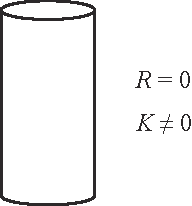
\includegraphics{Ch7_cylinder.pdf} }
\caption{For the cylinder, the intrinsic curvature vanishes ($R=0$), but the extrinsic curvature can be nonvanishing ($K\neq0$).}
\label{fig:cylinder} 
\end{figure}%
%%============

For example, consider a cylinder (\fig{cylinder}). The cylinder has no intrinsic curvature $R=0$ since the cylinder is just a flat space with a periodic boundary condition. But the cylinder is ``curved." This is the curvature which arises by embedding it into the three-dimensional space. This is the extrinsic curvature. In cylindrical coordinates
\be
%
ds^2 = dz^2+ dr^2+ r^2 d\theta^2~,
%\label{eq:}
%
\ee
the cylinder is the $r=\text{(constant)}$ surface. Then, $n^r=1$, $\gamma_{\mu\nu}=\text{diag}(1,r^2)$, and $\sqrt{\gamma}=r$, so the extrinsic curvature is indeed nonvanishing $K=1/r$.

In general relativity, one considers the extrinsic curvature of a surface when one embeds the surface into a spacetime or when one discusses the canonical formalism (one slices the spacetime into a series of spacelike hypersurfaces). In our case, we are talking of the extrinsic curvature of the four-dimensional timelike hypersurface sliced at $u=\text{(constant)}$ of the five-dimensional AdS black hole. This hypersurface is the spacetime where the boundary gauge theory lives.

For the SAdS$_5$ black hole, $n^u=-uh^{1/2}$ and $\sqrt{\gamma} = u^{-4}h^{1/2}$, so
% 2012/11/27����
%SAdS$_5$ �u���b�N�z�[���ɑ΂��ẮC$N^{-1}=uh^{1/2}$, $\sqrt{\gamma} = u^{-4}h^{1/2}$ �Ȃ̂�
\be
%
\action_\text{GH} =
 \left. 2uh^{1/2}\left[ u^{-4}h^{1/2} \right]'  \right|_{u=0} 
\xrightarrow{u\rightarrow0}{}
%\stackrel{u\rightarrow0}{\rightarrow}
 \left. -\frac{8}{u^4} + 4 \right|_{u=0}~.
\label{eq:GH_free_bdy}
%
\ee
Note that the Gibbons-Hawking action also diverges as $u\rightarrow0$.
%�M�{���Y-�z�[�L���O��p��������U�̊�^�����邱�Ƃɒ��ӁD

%%------------------
\subsubsection*{The counterterm action
%���E��p
}\label{sec:counter_free}
%%------------------

As we saw above, the bulk action and the Gibbons-Hawking action diverge as $u\rightarrow0$. To cancel the divergence, we add to the action another surface term, the \keyword{counterterm action}. 

In AdS/CFT, this divergence is interpreted as the ultraviolet divergence of the dual field theory. In the dual field theory, it is clear how to handle the divergence. One carries out the renormalization and adds a finite number of local counterterms to the bare action. Following this field theory prescription, we add a counterterm action in order to have a finite gravitational partition function. This procedure is known as the \keyword{holographic renormalization}%
\footnote{See, \eg, Ref.~\cite{Skenderis:2002wp} for a review of the holographic renormalization. The counterterm action contains the AdS scale $L$, so one cannot regulate the divergence if the spacetime is not asymptotically AdS. In particular, one cannot use this prescription for asymptotically flat black holes such as the Schwarzschild black hole. See \sect{HP} for a prescription of such a case.}. 
%���łɂ݂��悤�ɁC�o���N��p�C�M�{���Y-�z�[�L���O��p�� $u\rightarrow0$ �Ɍ��Ŕ��U����DAdS/CFT�̗���ł́C���̔��U�͑Ή������̗��_�̎��O���U�Ƃ��ĉ��߂����D���̏ꍇ�C���U������������@�͖��炩�ŁC��p�ɋǏ��I�ȑ��E����L���‰�����΂悢�D���̏�̗��_�̏����ɂȂ��炦�āC�d�͗��_�̕��z�֐���L���ɂ��邽�߂�{\bf ���E��p}\index{�������‚��悤@���E��p}��������D���̎葱����{\bf �z���O���t�B�b�N���荞��}\index{�ق낭��ӂ��‚����肱��@�z���O���t�B�b�N���荞��}�iholographic renormalization�j�ƌ���%
%\footnote{���E����AdS�X�P�[��$L$���܂ނ��߁C�Q�ߓI��AdS����ł͂Ȃ��ꍇ�C���̕��@�Ŕ��U���������邱�Ƃ͂ł��Ȃ��D�Ƃ��ɁC�ʏ�̑Q�ߓI���R�ȃu���b�N�z�[���i���Ƃ��΃V�������c�V���h�E�u���b�N�z�[���j�ɑ΂��Ďg���Ȃ��D���̏ꍇ�̏�����1�‚ɂ‚��Ă�\sect{HP}�ŋc�_����D}�D

Thus, the counterterm action is chosen so that
%���������āC���E����
\begin{itemize}

\item It is written only in terms of boundary quantities ($\gamma_{\mu\nu}$ and the quantities made of $\gamma_{\mu\nu}$ such as the Ricci scalar%
\footnote{Readers should not confuse $\cR$ with $R$, the Ricci scalar in the bulk spacetime. $R_{MN}$ is a tensor in $(p+2)$-dimensions, and $\cR_{\mu\nu}$ is a tensor in the $(p+1)$-dimensions.}  
$\cR$). 
%���E��̗ʂ݂̂ŏ������i$\gamma_{\mu\nu}$ ����т��ꂩ���������b�`�E�X�J���[$\cR$�Ȃ�%
%\footnote{������o���N���_�̃��b�`�E�X�J���[$R$�ƍ������Ă͂����Ȃ��D$R_{MN}$ �� $(p+2)$ �����̃e���\���ł���C$\cR_{\mu\nu}$ �� $(p+1)$ �����̃e���\���ł���D}�j�D

\item It consists of only a finite number of terms.
%�L���‚̍�����Ȃ�D

\item The coefficients of these terms are chosen once and for all in order to cancel divergences.
%�����̍��̌W���́C���U���������߂ɓK�؂ɑI�΂��D

\end{itemize}
When $p \leq 5$, the counterterm action is given by
%$p \leq 5$ �̂Ƃ��́C���E����
\begin{align}
%
\action_\text{CT} &= \frac{1}{16\pi G_{p+2}} \int  d^{p+1}x\, \sqrt{\gamma} 
  \left\{ 
  \frac{2p}{L} 
  + \frac{L}{p-1}\cR \right. 
\nonumber \\
& %\hspace{2cm} 
 \left. - \frac{L^3}{(p-3)(p-1)^2} \left(\cR^{\mu\nu}\cR_{\mu\nu} - \frac{p+1}{4p}\cR^2\right)
+ \cdots
\right\}.
%\label{eq:}
%
\end{align}
The above terms are enough to cancel power-law divergences for $p \leq 5$, but one may need the other terms to cancel log divergences. For black holes with planar horizon, $\cR_{\mu\nu}=0$, so only the first term contributes to thermodynamic quantities:
%$p \leq 5$ �̂Ƃ��́C�x�L���U�������̂ɏ�L�̍��ŏ\���ł��邪�C�ΐ����U���������߂̐V���ȍ����K�v�ɂȂ�ꍇ������D�v���i�[�E�z���C�Y���̏ꍇ�C$\cR_{\mu\nu}=0$ �Ȃ̂ŁC���ۂɂ͏����݂̂��M�͊w�ʂɂ͊�^����F
\be
%
\action_\text{CT} = \left. 6u^{-4}h^{1/2} \right|_{u=0} 
\xrightarrow{u\rightarrow0}{}
%\stackrel{u\rightarrow0}{\rightarrow}
 \left. \frac{6}{u^4} - 3 \right|_{u=0}~.
\label{eq:counter_free_bdy}
%
\ee

%%------------------
\subsubsection*{The partition function and thermodynamic quantities
%���z�֐��ƔM�͊w��
}%\label{sec:}
%%------------------

To summarize our results \eqref{eq:bulk_free_bdy}, \eqref{eq:GH_free_bdy}, and \eqref{eq:counter_free_bdy},
%����܂ł̌��� \eqref{eq:bulk_free_bdy}, \eqref{eq:GH_free_bdy}, \eqref{eq:counter_free_bdy} ���܂Ƃ߂�ƁC
%\begin{subequations}
%\label{eq:}
\begin{align}
%
\action_\text{bulk} &= \left. \frac{2}{u^4} - 2 \right|_{u=0}~, \\
\action_\text{GH} &=  \left.  -\frac{8}{u^4} + 4 \right|_{u=0}~, \\
\action_\text{CT} &=  \left.  \frac{6}{u^4} - 3 \right|_{u=0}~.
%\label{eq:}
%
\end{align}
%\end{subequations}
Combining these results, we get a simple result $\action_\text{bulk} + \action_\text{BH} + \action_\text{CT} = -1$ after all these computations. Recovering dimensionful quantities, we get
%���������킹�Ď����ʂ𕜊�������ƁC
\be
%
\SosE =  - \frac{\beta V_3}{16\pi G_5} \frac{r_0^4}{L^5}~.
%\label{eq:}
%
\ee
The on-shell action is related to the partition function $Z$ and the free energy \index{free energy} $F$ as
%on-shell ��p�ƁC���z�֐�����ю��R�G�l���M�[\index{���䂤���˂邫�[@���R�G�l���M�[}�̊֌W�́C
\be
%
Z = e^{-\SosE}~, \quad
\SosE = \beta F~.
%F= -T \ln Z = \frac{\SosE}{\beta}~.
%
\ee
Then, the free energy becomes
%$T=r_0/(\pi L^2)$ ���g���ƁC
\be
%
F =  - \frac{V_3}{16\pi G_5} \frac{r_0^4}{L^5} 
= - \frac{(\pi L T)^4}{16 \pi G_5 L} V_3 
= -\frac{1}{8}\pi^2 N_c^2 T^4 V_3~,
%\label{eq:}
%
\ee
where we used $T=r_0/(\pi L^2)$. Thermodynamic quantities are then derived from the free energy as
%���̎��R�G�l���M�[���C�M�͊w�ʂ́C
%\begin{subequations}
%\label{eq:}
\begin{align}
%
s &= - \frac{1}{V_3}\del_T F 
= \frac{(\pi L T)^3}{4G_5} = \frac{1}{4G_5} \left(\frac{r_0}{L}\right)^3
= \frac{1}{2}\pi^2 N_c^2 T^3~, \\
P &= - \del_{V_3} F
= \frac{(\pi L T)^4}{16\pi G_5 L} = \frac{1}{16\pi G_5 L} \left(\frac{r_0}{L}\right)^4
= \frac{1}{8}\pi^2 N_c^2 T^4~, 
\label{eq:pressure_sads} \\
\varepsilon &= \frac{F}{V_3} + T s
= \frac{3(\pi L T)^4}{16\pi G_5 L} = \frac{3}{16\pi G_5 L} \left(\frac{r_0}{L}\right)^4
= \frac{3}{8}\pi^2 N_c^2 T^4~.
%\label{eq:}
%
\end{align}
%\end{subequations}

\endofsection

	   \begin{thebibliography}{99}

%
% Chap_AdSBH 
%

% added
%\cite{York:1986it}
\bibitem{York:1986it}
  J.~W.~York, Jr.,
  ``Black hole thermodynamics and the Euclidean Einstein action,''
  Phys.\ Rev.\  {\bf D33 } (1986)  2092.
  
%\cite{Gubser:1996de}
\bibitem{Gubser:1996de}
  S.~S.~Gubser, I.~R.~Klebanov and A.~W.~Peet,
  ``Entropy and temperature of black 3-branes,''
  Phys.\ Rev.\  {\bf D54 } (1996)  3915
  [hep-th/9602135]. 
 
% added
%\cite{Balasubramanian:1999re}
\bibitem{Balasubramanian:1999re}
  V.~Balasubramanian and P.~Kraus,
  ``A Stress tensor for Anti-de Sitter gravity,''
  Commun.\ Math.\ Phys.\  {\bf 208 } (1999)  413 
  [hep-th/9902121].
  
% added
%\cite{Skenderis:2002wp}
\bibitem{Skenderis:2002wp}
  K.~Skenderis,
  ``Lecture notes on holographic renormalization,''
  Class.\ Quant.\ Grav.\  {\bf 19} (2002) 5849
  [hep-th/0209067].
  %%CITATION = HEP-TH/0209067;%%

\end{thebibliography}
	%\documentclass[11pt]{jarticle} %%% �A���R�����g
\ifx\nameofpaper\undefined %%% ���� main.tex ���ǂ܂�Ă��Ȃ����
  \usepackage{macro_natsuume} %%% �����p�̃}�N���t�@�C����ǂݍ��݁C
  \def\beginsection{\section*}
  \def\endofsection{\end{document}} %%% \endofsection = \bye �ƒ�`
  \input draft_header.tex
\else %%% �����łȂ����
  \def\beginsection{\chapter}
  \def\endofsection{\endinput} %%% \endofsection = \endinput �ƒ�`
\fi


%%%%%%%%%
\beginsection{AdS/CFT - adding probes
%AdS/CFT-�v���[�u���������ꍇ
}\label{chap:wilson}
%%%%%%%%%

%\begin{flushright}
%        \today\\
%\end{flushright}

\begin{quote}
In real experiments, one often adds ``probes" to a system to examine its response. Or one adds impurities to a system to see how they change the properties of the system. In this chapter, we discuss how to add probes in AdS/CFT. As a typical example, we add ``quarks" to gauge theories as probes and see the behavior of quark potentials.
%�����ł́C���΂��Όn�Ɂu�v���[�u�v�������āC�v���[�u�ւ̔����𒲂ׂ�D�܂��C��l�Ȍn�ɕs�����������Čn�̐������ǂ��ς�邩�𒲂ׂ邱�Ƃ�����D�{�͂ł́CAdS/CFT�ł��̂悤�ȃv���[�u����������@�ɂ‚��ċc�_����D��\�I�ȗ�Ƃ��āC�Q�[�W���_�Ƀv���[�u�Ƃ��ẴN�H�[�N�������C�N�H�[�N�E�|�e���V�����̐U��܂����݂邱�Ƃɂ���D
\end{quote}

Coupling new degrees of freedom to the original system often arises new phenomena. Adding some new degrees of freedom to AdS/CFT should be also interesting. This is practically important as well. The \Nfour\ SYM is clearly insufficient to mimic real worlds completely since, \eg, it does not have quarks. 

In string theory, there are various fields and branes, so one may would like to add them. The resulting geometries or solutions have been known for some cases, but it is in general very difficult to solve the Einstein equation when there are multiple number of fields and branes. 

So, one often adds them as ``probes." This is just like the particle motion analysis in curved spacetime (Sects.~\ref{sec:classic_tests} and \ref{sec:geodesics_AdS}). One fixes the background geometry and considers the case where the backreaction of the probe onto the geometry is negligible. 

In this chapter, as a typical example, we add ``quarks" to large-$\Nc$ gauge theories as a probe and analyze quark potentials. In \sect{H^3}, we see another example of a probe system, holographic superconductors.

%%%%%%%%%
\section{Basics of Wilson loop
%�E�B���\�����[�v�̏���
}%\label{sec:}
%%%%%%%%%

The \keyword{Wilson loop} is an important observable in gauge theory, and it represents the quark-antiquark potential physically. As an example, consider a $U(1)$ gauge theory with gauge transformation given by
%�E�B���\���E���[�v�́C�Q�[�W���_�̏d�v�ȃI�u�U�[�o�u����1�‚ł���C�����I�ɂ̓N�H�[�N�E���N�H�[�N�|�e���V����������킵�Ă���D��Ƃ��āC$U(1)$�Q�[�W���_���l����D�Q�[�W�ϊ��́C
\begin{align}
%
\phi(x) &\rightarrow e^{i\alpha(x)} \phi(x)~, \\
A_\mu(x) &\rightarrow A_\mu(x) + \del_\mu \alpha(x)~.
%\label{eq:}
%
\end{align}
A nonlocal operator such as $\phi(x)\phi^*(y)$ is not gauge invariant in general and is not an observable. But the following quantity is gauge-invariant:
\be
%
\phi(x) e^{i \!\int_P dx^\mu A_\mu } \phi^*(y)~,
%\label{eq:}
%
\ee
where $P$ is an arbitrary path from point $x$ to $y$ [\fig{path}]. It transforms as
%�ŗ^������D�Ǐ��I�łȂ��I�y���[�^�[�C���Ƃ��� $\phi(x)\phi^*(y)$ �͈�ʂɃQ�[�W�s�ςł͂Ȃ��C�I�u�U�[�o�u���ł͂Ȃ��D�������ȉ��̗ʂ̓Q�[�W�s�ςł���F
%\mathindent=0zw % <-- [1]
\begin{align}
%
\phi(x) e^{i \!\int_P dx^\mu A_\mu } \phi^*(y)
& \rightarrow
\phi(x) e^{i\alpha(x)} e^{i \!\int_P dx^\mu (A_\mu+\del_\mu \alpha) } e^{-i\alpha(y)} \phi^*(y)\\
& = \phi(x) e^{i \!\int_P dx^\mu A_\mu } \phi^*(y)~.
%\label{eq:}
%
\end{align}
%\mathindent=2zw % <-- [2] �f�t�H���g
%$P$�͓_$x$��$y$���‚Ȃ��C�ӂ̌o�H�ł��� [ \fig{path} ]�D���邢�́C$P$�Ƃ��ĕ‹Ȑ����Ƃ�΁C$W_P$ �����ŃQ�[�W�s�ςɂȂ�D�����ňȉ��̂悤�ɃI�y���[�^�[���`����F
Or if one takes a closed path $P$, $W_P$ itself is gauge invariant. Thus, we define the following operator:
\begin{alignat}{2}
%
W_P(x,y) &= e^{i \int_P dx^\mu A_\mu }  \quad & (\text{Wilson line})~, \\
W_P(x,x) &= e^{i \oint dx^\mu A_\mu }  \quad & (\text{Wilson loop})~.
%\label{eq:}
%
\end{alignat}

%%============
\begin{figure}[tb]
\centering
\subfigure[]{
\scalebox{0.75}{ 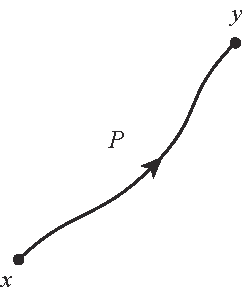
\includegraphics{Ch8_path.pdf} }
\label{fig:path}} \qquad
\subfigure[]{
\scalebox{0.70}{ 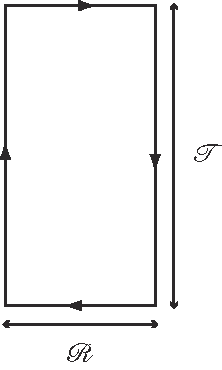
\includegraphics{Ch8_wilson.pdf} }
\label{fig:wilson}}
\vskip2mm
\caption{(a) Path $P$. (b) The Wilson loop represents a quark-antiquark pair.}
%(a) �o�H $P$�D (b) �E�B���\���E���[�v�̓N�H�[�N�E���N�H�[�N�΂�����킷�D
%\label{fig:path}
\end{figure}%
%%============

The Wilson loop represents the coupling of the gauge field to a test charge. Consider a charged particle with world-line $y^\mu(\lambda)$. The current is given by
%{\bf �E�B���\���E���[�v}\index{�����邻���[��@�E�B���\���E���[�v}�́C�e�X�g�d�ׂ̃Q�[�W��ւ̌���������킷�D���q���d�ׂ����ꍇ�C�J�����g��
\be
%
J^\mu(x) = \oint d\lambda\, \frac{dy^\mu}{d\lambda} \delta\left( x^\mu-y^\mu(\lambda) \right)~.
%\label{eq:}
%
\ee
The sign of the charge depends on the sign of $dy/d\lambda$. Here, we take $dy/d\lambda>0$ for a positive charge. For a given closed path, $dy/d\lambda$ can be both positive and negative, so we have both a positive charge and a negative charge [\fig{wilson}]. Namely, the closed path describes the process of creating a ``quark-antiquark pair" from the vacuum, pulling them a distance $\calR$ apart, interacting for time $\calT$, and annihilating them. If one uses $J^\mu$, the coupling of the gauge field to  the point particle action is written as $\delta\action = \int d^4x\, A_\mu J^\mu$. This perturbed action $\delta\action$ can be rewritten as the exponent of the Wilson loop:
%Using $J^\mu$, one can rewrite the exponent of the Wilson loop as a perturbed action $\delta\action$:
%�d�ׂ�$dy/d\lambda$�̕����Ō��܂�D�v���X�̓d�ׂɑ΂��C$dy/d\lambda>0$�ƂƂ��Ă���D�‹Ȑ� $y^\mu(\lambda)$ ���l����ƁC$dy/d\lambda$���������̕���������̂ŁC�v���X�ƃ}�C�i�X�̓d�ׂ�����킷���ƂɂȂ� [ \fig{wilson} ]�D�‚܂�C�‹Ȑ��́u�N�H�[�N�E���N�H�[�N�v���ΐ�������C$\calR$�̋�����$\calT$�̎��ԁC���ݍ�p���N�����C�܂��Ώ��ł���v���Z�X������킷�D$J^\mu$ ���g���ƁC�E�B���\���E���[�v�͍�p�̐ۓ����̌`�ɏ�����F
%\mathindent=0zw % <-- [1]
\be
%
\delta \action
= \!\int d^4x\, A_\mu(x) J^\mu(x) 
= \!\oint d\lambda\, \frac{dy^\mu}{d\lambda} A_\mu(y(\lambda))
= \!\oint dy^\mu A_\mu(y)~.
%\label{eq:}
%
\ee
%\mathindent=2zw % <-- [2] �f�t�H���g
Therefore, the Wilson loop represents a partition function in the presence of a test charge:
%���������āC�E�B���\���E���[�v�̓e�X�g�d�ׂ�����Ƃ��̕��z�֐�������킷�F
\be
%
\bra W_P \ket = \frac{Z[J]}{Z[0]}~.
%\label{eq:}
%
\ee

Such a partition function gives the quark-antiquark potential. Let us write the Euclidean partition function formally as
%���̂��Ƃ���C�E�B���\���E���[�v�̓N�H�[�N�E���N�H�[�N�΂̃|�e���V�����E�G�l���M�[��^���邱�Ƃ��킩��D���[�N���b�h���������z�֐����`���I��
\be
%
Z = \bras{f} e^{-H\calT} \kets{i}
%\label{eq:}
%
\ee
($\kets{i}$ and $\kets{f}$ are the initial state and the final state, respectively). If one uses a complete set of energy eigenstates $H \kets{n} = E_n \kets{n}$,
%�Ə����C���S�n$H \kets{n} = E_n \kets{n}$���g����
\be
%
Z = \sum_n e^{-E_n \calT} \norm{f}{n}\norm{n}{i} 
%\stackrel{\calT\rightarrow\infty}{\rightarrow} 
 \xrightarrow{\calT\rightarrow\infty}{} e^{-E_0 \calT}~.
%\label{eq:}
%
\ee
Thus, in the $\calT\rightarrow\infty$ limit, the Euclidean partition function is dominated by the ground state and gives the ground state energy. When the kinetic energy is negligible, it gives the quark-antiquark potential energy%
\footnote{From $\tE = it$, the Lorentzian action $\action_L$, the Euclidean action $\action_E$, and the potential $V$ are related to each other by $i \action_L = i\int dt (-V) = -\int d\tE V = - \action_E$.}.
Consequently,
%�‚܂�C���[�N���b�h���������z�֐��́C$\calT\rightarrow\infty$�̋Ɍ��Ŋ���Ԃ̃G�l���M�[��^����D�����āC�^���G�l���M�[�������ł���Ƃ��́C�|�e���V�����E�G�l���M�[��^����%
%\footnote{$\tE = it$ �̉��ŁC�~���R�t�X�L�[��p $\action_L$�C���[�N���b�h��p $\action_E$�C�|�e���V���� $V$ �̊֌W�́C$i \action_L = i\int dt (-V) = -\int d\tE V = - \action_E$�D}�D
%���������āC
\be
%
\bra W_P \ket \simeq e^{-V(\calR)\calT}~.
%\label{eq:}
%
\ee
One can show that the horizontal parts of \fig{wilson} are negligible in the large $\calT\rightarrow\infty$ limit.
%\fig{wilson}�̐��������� $O(\calR/\calT) \ll 1$�ł��邱�Ƃ�������D

When the quark is confined like QCD, the potential grows with the separation $\calR$, so $V(\calR) \simeq \sigma \calR (\calR \gg 1)$, where $\sigma$ is called the string tension. Then,
%QCD�̂悤�ɃN�H�[�N�̕‚����߂��N����ꍇ�C�|�e���V�����͋����ƂƂ��ɑ��傷��F$V(\calR) \simeq \sigma \calR (\calR \gg 1)$�D������$\sigma$ �̓X�g�����O�E�e���V�����ƌĂ΂��D���������āC
\be
%
\bra W_P \ket \simeq e^{-O(\calR\calT)} = e^{-\sigma A}~.
%\label{eq:}
%
\ee
The exponent is proportional to the area of the Wilson loop $A = \calR\calT$. This behavior is known as the \textit{area law}\index{area law (Wilson loop)}. An unconfined potential behaves differently. The Coulomb potential decays with the separation, and one can show that 
%���[�v�̖ʐ�$A = \calR\calT$�ɔ�Ⴗ�邱�̐U��܂���{\bf �ʐϑ�}\index{�߂񂹂����������邻��@�ʐϑ��i�E�B���\���E���[�v�j}�ƌ����D����C�����ƂƂ��Ƀ|�e���V��������������N�[�����͂̏ꍇ�́C
\be
%
\bra W_P \ket \simeq e^{-O(\calR)}
\quad (\text{when } \calR=\calT \gg 1)~.
%\label{eq:}
%
\ee
This is known as the perimeter law. In this way, the Wilson loop provides a criterion for the confinement. 
%�ƐU��܂��C�����``Perimeter law"�ƌ����D���̂��߃E�B���\���E���[�v�́C�‚����߂̔��������^����D

Here, we consider only the $U(1)$ gauge theory, but a similar discussion can be done for a Yang-Mills theory.
%�����ł͊ȒP�̂��߂�$U(1)$�Q�[�W���_�������l���Ă������C���l�̋c�_�̓���-�~���Y���_�ɑ΂��Ă���������D


%%%%%%%%%
\section{Wilson loops in AdS/CFT: intuitive approach
%AdS/CFT�ł̃E�B���\�����[�v�F���ϓI����
}\label{sec:wilson_intuitive}
%%%%%%%%%


%%-------------------------------------
%\subsection{��{�I�ȍl����}\label{sec:deconfine}
%%-------------------------------------

%%============
%\begin{figure}[tb]
%\centering
%\hspace{0.25in}
%\scalebox{0.5}{ 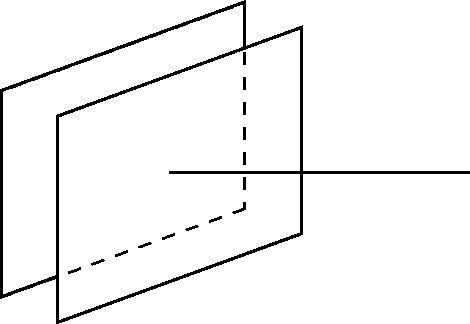
\includegraphics{Ch8_quark.pdf} }
%\vskip2mm
%\caption{A long string represents a massive ``quark.''}
%�����X�g�����O�́C�d���N�H�[�N������킷�D
%\label{fig:quark}
%\end{figure}%
%%============

%%============
\begin{figure}[tb]
\centering
\subfigure[]{
\scalebox{0.75}{ 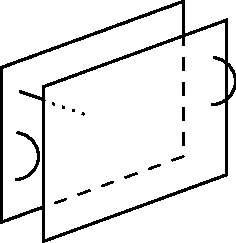
\includegraphics{Ch5_SYM.pdf} }
\label{fig:Dbrane_SYM_again} } \qquad
\subfigure[]{
\scalebox{0.5}{ 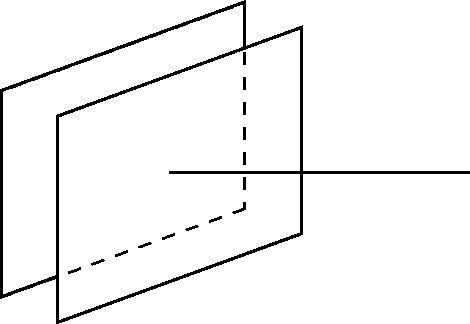
\includegraphics{Ch8_quark.pdf} }
\label{fig:quark} }
\vskip2mm
\caption{
(a) An open string can have endpoints on a D-brane. The $N_c$ coincident D-branes represent a $SU(N_c)$ gauge theory. (b) A long string represents a massive ``quark.''
}
%\label{fig:Dbranes_again}
\end{figure}%
%%============

Let us consider the Wilson loop in AdS/CFT. The Wilson loop in AdS/CFT gives a typical example of adding a probe system to the original system. The AdS/CFT results can be understood intuitively. So, before we go through an actual computation, we first explain what kind of results one can expect in various situations. Then, we confirm our intuitive explanation via an actual computation.
%AdS/CFT�ŃE�B���\���E���[�v���l���悤�DAdS/CFT�ł̌��ʂ́C�萫�I�ɂ͒��ϓI�ɗ����ł���D�����ŁC���ۂɌv�Z����O�ɁC���܂��܂ȏ󋵂łǂ̂悤�Ȍ��ʂ����҂����̂����������D���̂��ƂŁC���ϓI�ȗ��������ۂ̌v�Z�ŗ��Â���D

The matter fields in the ${\cal N}=4$ SYM are all in the adjoint representation. So, one first has to understand how to realize the fundamental representation\index{fundamental representation} such as  a quark in AdS/CFT. Below, we describe one simple way to add such matter. 
%${\cal N}=4$ �Q�[�W���_�ɂ�����镨����͐����\�������Ȃ̂ŁC�܂��N�H�[�N�̂悤�Ȋ�{�\��\index{���ق�Ђ悤����@��{�\��}�̕������AdS/CFT�łǂ������邩�l����K�v������D�����ł�1�‚̊ȒP�ȕ��@���c�_����

To do so, recall how the adjoint representation appeared for the D-brane [\fig{Dbrane_SYM_again}]. 
%let us go back to \fig{Dbranes}. 
The open strings can have endpoints on a D-brane, but when there are multiple number of D-branes, an open string can have endpoints in various ways; there are $N_c^2$ possibilities. This means that the string transforms as the adjoint representation of $SU(N_c)$ gauge theory. 
%\fig{Dbrane}�ɖ߂낤�D�J����D�u���[����ɒ[�_�����‚��CD�u���[��������������ƁC�[�_�̒u������$N_c^2$�������D���̂��Ƃ́C�J��������킷�ꂪ$SU(N_c)$�̐����\���ɑ����邱�Ƃ��Ӗ������D

Now, consider an infinitely long string [\fig{quark}]. In this case, the string can have endpoints in $N_c$ different ways. This means that the string transforms as the fundamental representation of $SU(N_c)$ gauge theory. In this sense, such a long string represents a ``quark." Such a string has an extension and tension, so the string has a large mass, which means that the long string represents a heavy quark. We discuss the Wilson loop in AdS/CFT using such a string.
%����C�����ɒ����X�g�����O���l����Ɓi\fig{quark}�j�C�X�g�����O�̒[�_�̒u������$N_c$�ł���D���̂��Ƃ͏ꂪ��{�\���ɑ����邱�Ƃ��Ӗ�����D���̈Ӗ��ŁC�����X�g�����O�́u�N�H�[�N�v������킷�D�X�g�����O�͒��͂������L�тĂ���̂ŁC���̂悤�ȃX�g�����O�͖����ɏd�����ʂ����D�‚܂�C���̂悤�ȃX�g�����O�́C�����ɏd���N�H�[�N������킷�̂ł���D�ȉ��ł́C���̂悤�ȃX�g�����O���g���āC�E�B���\���E���[�v���c�_���邱�Ƃɂ���D

We saw earlier that the string model of QCD does not describe potentials other than the confining potential (Problem 2 of \sect{prehistory}). However, one can avoid this problem in AdS/CFT, and one can get the Coulomb potential which appears at short distances in QCD. The AdS/CFT result differs from the simple string model one essentially because of the curved spacetime effect as discussed below. Note that we avoided Problem 1 of \sect{prehistory} by the same trick.
%�ȑO�C�����͂̃X�g�����O�͌^�̌��_�Ƃ��āC�‚����߈ȊO�̃|�e���V����������킳��Ȃ��Ƃ����_���������i\sect{prehistory}�̖��2�j�D�Ƃ��낪�CAdS/CFT�ł͂��̖�������ł��āCQCD�̒Z�����ŏo�Ă���悤�ȃN�[�����E�|�e���V�������o�Ă��邱�Ƃ��݂�DAdS/CFT�ƒP���ȃX�g�����O�͌^���Ⴄ���_�ɂȂ�̂́C\sect{prehistory}�̖��1������������R�Ɗ�{�I�ɂ͓����ŁC�ȉ��ł݂�悤�ɋȂ���������̌��ʂł���D

First, we discuss the simplest case, the pure AdS case, to understand the basic idea of the AdS/CFT quark potential. In this case, one gets only the Coulomb potential. We then consider a more generic AdS spacetime and get a confining potential as well. Also, if we consider a black hole, we can recover behaviors in plasma phase.
%�܂��CAdS/CFT�ł̃N�H�[�N�E�|�e���V�����̊�{�I�ȍl�����𗝉����邽�߂ɁC��ԊȒP��AdS����̏ꍇ���l����D���̏ꍇ�̓N�[�����E�|�e���V���������o�Ȃ��D���̂��ƁC�����ƈ�ʓI��AdS������l����ƁC�‚����߃|�e���V�������o�ĕ‚����߂�����킳��邱�ƁC�܂��u���b�N�z�[���̏ꍇ���l����ƃv���Y�}���ł̐U��܂�������킳��邱�Ƃ��݂Ă����D

%%-------------------------------------
\subsubsection*{The pure AdS spacetime
%AdS����̏ꍇ
}%\label{sec:pure_AdS}
%%-------------------------------------

%%============
\begin{figure}[tb]
\centering
%\hspace{0.25in}
\scalebox{0.75}{ 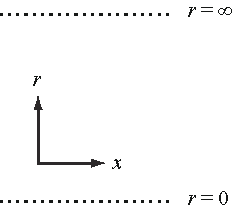
\includegraphics{Ch8_potential1.pdf} }
\vskip2mm
\caption{Schematically drawn AdS spacetime. The horizontal direction represents one of three-dimensional space the gauge theory lives. The vertical direction represents the AdS radial coordinate. The radial coordinate extends from $r=0$ to $r=\infty$, but we draw in a compact region for illustration.}
%�͎��I�ɕ`����AdS����D���������̓Q�[�W���_�̏Z��3������Ԃ̂P�‚�����킵�C����������AdS����̓��a����������킷�D���a�����́C$r=0$ ���� $r=\infty$ �܂Ŋg�����Ă��邪�C�}������s����k�߂ĕ`���Ă���D}
\label{fig:potential1}
\end{figure}%
%%============

The AdS metric in \poincare\ coordinates is written as
%���炽�߂�AdS����̌v�ʂ������Ɓi�|�A���J�����W�j�C
%\mathindent=0zw %
\be
ds^2 = \left( \frac{r}{L} \right)^2(-dt^2+dx^2+\cdots)~.
\label{eq:metric_AdS}
\ee
%\mathindent=2zw %
The line element has the factor $r^2$. We measure the gauge theory time and distance using $t$ and $x$, but they differ from the proper time and distance of the AdS spacetime. This is the important point, and the qualitative behavior of the quark potential can be understood using this fact.
%�Ɛ��f��$r^2$�̈��q���������Ă���_�������ł���D�Q�[�W���_�ł̎��ԁE������ $t$, $x$�̒l�ő�����i�‚܂�$r^2$�̈��q�������Ȃ��j�D�������C����͋Ȃ���������{���ł̐��f�Ƃ͈Ⴄ�Ƃ����_���|�C���g�ł���D�N�H�[�N�E�|�e���V�����̒萫�I�ȐU��܂��́C���̂��Ƃ������痝���ł���D

Figure~\ref{fig:potential1} shows the AdS spacetime schematically. Denote the quark-antiquark separation as $\Delta x=\calR$. The quark-antiquark pair is represented by a string which connects the pair. The string has the tension, so the tension tends to minimizes the string length. At first glance, one would connect the pair by a straight string at  $r=\infty$ (\fig{potential2}). But this does not minimize the string length. This is because the coordinate distance does not represent a true distance (proper distance) in a curved spacetime. The figure does not show the proper length properly, so one needs a care. For the AdS spacetime, the proper length of the string actually gets shorter if the string goes inside the AdS spacetime ($r\neq\infty$). The line element has the factor $r^2$, so the proper length $r\Delta x$ gets shorter near the origin.
%\fig{potential1}��AdS�����͎��I�ɕ`�������̂ł���D�N�H�[�N�Ԃ̋�����$\calR$�Ƃ���i$\Delta x=\calR$�j�D�N�H�[�N�E�|�e���V�����̓N�H�[�N���‚Ȃ��X�g�����O�ɂ���Ă���킳���D�X�g�����O�͒��͂������Ă���̂ŁC�X�g�����O�̒������ŒZ�ɂȂ낤�Ƃ���D�ꌩ����ƁC�N�H�[�N�� $r=\infty$ �Ő����ɐL�т��X�g�����O�ł‚Ȃ���Ηǂ������Ɏv����i\fig{potential2}�j�D�������C����ł̓X�g�����O�̒����͍ŒZ�ɂ͂Ȃ�Ȃ��D�Ȃ���������ł́C���W�Ԋu���K�������{���̋����i�ŗL�����j������킷�킯�ł͂Ȃ�����ł���D���̐}�͌ŗL������K�؂ɂ���킵�Ă͂��Ȃ��̂ŁC���̓_���ӂ��K�v�ł���D���́CAdS����̏ꍇ�C�������񎞋�̓����i$r\neq\infty$�j�ɓ����������X�g�����O�̌ŗL�����͒Z���Ȃ�%
%\footnote{$x$�����̐��f�ɂ�$r^2$�̈��q���������Ă���̂ŁC���_�߂��̕����ŗL����$r\Delta x$�͒Z���Ȃ�D}�D

%%============
\begin{figure}[tb]
\centering
%\hspace{0.25in}
\scalebox{0.75}{ 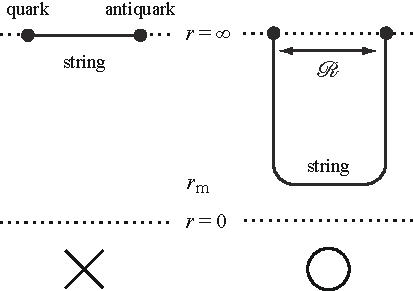
\includegraphics{Ch8_potential2.pdf} }
\vskip2mm
\caption{The straight string is not the lowest energy state (left), and the string which goes inside the AdS spacetime is the lowest energy state (right).}
%�����ɐL�т��X�g�����O�i���j�͍Œ�G�l���M�[��Ԃł͂Ȃ��CAdS����̓����ɓ��������̂��Œ�G�l���M�[��ԂɂȂ�D}
\label{fig:potential2}
\end{figure}
%%============

%%============
\begin{figure}[tb]
\centering
%\hspace{0.25in}
\scalebox{0.75}{ 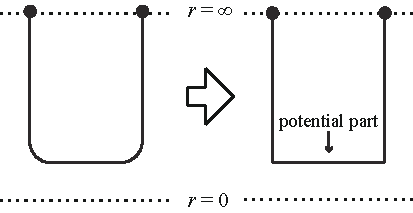
\includegraphics{Ch8_potential3.pdf} }
\vskip2mm
\caption{The string which connects the quark pair (left) is approximated by a rectangular string. The energy of the horizontal string gives the quark potential. }
%�N�H�[�N���‚Ȃ��X�g�����O�i���j���ߎ��I�ɒ����`�̃X�g�����O�ł���킷�i�E�j�D�����ɐL�т��X�g�����O�̃G�l���M�[���C�N�H�[�N�E�|�e���V����������킷�D}
\label{fig:potential3}
\end{figure}%
%%============

According to the analysis of \sect{wilson_details}, this string is roughly divided into two parts: the part the string extends vertically, and the part the string extends horizontally. So, for simplicity, let us approximate the configuration by a rectangular string (\fig{potential3}). Only the horizontal string contributes to the quark potential. This part varies as we vary the quark separation $\calR$. On the other hand, the vertical string does not vary much. This part simply describes the quark mass. 
%\sect{wilson_details}�̏ڂ�����͂ɂ��ƁC���̃X�g�����O�͑�G�c�Ɍ�����2�‚̕����ɕ�������D���̕����͂قڐ����ɐL�т������ŁC���̕����͂ނ���قڐ����ɐL�т������ł���D���������āC�����ł͊ȒP���̂��߂ɁC���̃X�g�����O���ߎ��I�ɒ����`�̃X�g�����O�Œu�������邱�Ƃɂ���i\fig{potential3}�j�D���̂����C�N�H�[�N�E�|�e���V�����ɑ�������̂́C���̕����ł���D�N�H�[�N�Ԃ̋��� $\calR$ ���g�����Ƃ��ɕω�����̂͂��̕���������ł���D����C���������͂��܂�ω����Ȃ��̂ŁC���̕����͂ق��̃N�H�[�N�Ƃ͖��֌W�ŁC���Ƃ��ƃN�H�[�N�����Ž��ʂ�����킵�Ă���D

%%============
\begin{figure}[!tb]
\centering
%\hspace{0.25in}
\scalebox{0.75}{ \includegraphics{Ch8_potential4.pdf} }
\vskip2mm
\caption{The behavior of the string as we vary the quark separation. The larger $\calR$ lowers the string turning point $\rmin$ as $\rmin \propto 1/\calR$.}
%�N�H�[�N�Ԃ̋�����ς����Ƃ��̃X�g�����O�̐U��܂��D$\calR$��傫������ƁC�X�g�����O�̉��[ $\rmin$ �� $\rmin \propto 1/\calR$ �̂悤�ɉ������Ă���D}
\label{fig:potential4}
\end{figure}%
%%============

We need a little more information to compute the potential. The explicit computation shows that the string turning point $r=\rmin$ behaves as
%�|�e���V�������v�Z����ɂ́C����������񂪕K�v�ł���D�܂��C���ۂɌv�Z����ƃX�g�����O�̉��[ $r=\rmin$ ��
\be
%
\rmin \propto L^2/\calR
\label{eq:r_min}
%
\ee
(\fig{potential4}). Also, the line element \eqref{eq:metric_AdS} gives two consequences. First, the proper length of the horizontal string is $(r/L)\calR$, so the string energy $E(r)$ is given by
%�ƂȂ�i\fig{potential4}�j�D�܂����f \eqref{eq:metric_AdS} ����Q�‚̋A�����l������D���ɁC���������̌ŗL������ $(r/L)\calR$ �Ȃ̂ŁC�X�g�����O�̃G�l���M�[�� 
\be
%
E(r) \propto \left( \frac{r}{L} \right) \calR~.
\label{eq:proper_energy}
%
\ee
Second, this energy is the proper energy and not the gauge theory energy. The timelike direction also has the factor $r^2$ as in \eq{metric_AdS}. The gauge theory time is the coordinate time $t$ not the proper time. As a result, the gauge theory energy differs from the proper energy $E(r)$. From \eq{metric_AdS}, the proper time $\tau_r$ is related to the gauge theory time by $\tau_r=(r/L) t$, so the proper energy is related to the gauge theory energy $E_t$ by
%�ƂȂ�D���ɁC���̃G�l���M�[ $E_{5}$ ��5��������̗���ł̃G�l���M�[�ŁC�Q�[�W���_�̗���ł̃G�l���M�[�ł͂Ȃ��D\eq{metric_AdS}�ɂ���悤�ɁC���ԕ����ɂ�$r^2$���������Ă��邩��ł���D�Q�[�W���_�̗���ł̎��Ԃ͂����܂�$t$�Ȃ̂ŁC$E_{5}$���Q�[�W���_�̃G�l���M�[$E_\text{gauge}$�ɒ����K�v������i\sect{interpretation}�j�D\eq{metric_AdS}����C5�����ł̌ŗL����$\tau_{5}$�ƃQ�[�W���_�̎���$t$�̂�������$\tau_{5}=(r/L) t$�̊֌W�����藧�‚̂ŁC�G�l���M�[�̊֌W�͂��́u�t�v�‚܂�
\be
%
E_t = \left( \frac{r}{L} \right) E(r)~.
\label{eq:UV/IR2}
%
\ee
This is the UV/IR relation\index{UV/IR relation} in \sect{interpretation} \cite{Susskind:1998dq,Peet:1998wn}. Thus, the potential is given by
%�ƂȂ�D�����ōŏI�I�ɂق����|�e���V������\eq{r_min}���g����
\begin{align}
%
E_t &=  \left( \frac{\rmin}{L} \right) E(r)
\propto \left( \frac{\rmin}{L} \right)^2 \calR \\
&\propto \frac{L^2}{\calR}~,
%&\simeq O(L^2/\calR)~.
\label{eq:coulomb}
%\label{eq:}
%
\end{align}
where we also used \eq{r_min}. This result \cite{Rey:1998ik,Maldacena:1998im} has two important points:
\begin{enumerate}
\item
First, we obtained the Coulomb potential $E \propto 1/\calR$ not the confining potential $E \propto \calR$. Namely, the string connecting the quark-antiquark pair does not necessarily implies a confining potential, but it can describe an unconfining potential using the curved spacetime. \textit{In this way, we resolved Problem 2 of the string model in \sect{prehistory}.} But then, how can we describe the confining potential in AdS/CFT? We will discuss this point below. 
%���̂悤�ɃN�[�����^�̃|�e���V�����ƂȂ�%
%\footnote{�{���̃N�[�����E�|�e���V�����Ȃ�$E \simeq -1/\calR$�ƂȂ�͂������C���̕��@�ł͕����܂ł͍Č��ł��Ȃ��D����́C�X�g�����O��e���ۂ�\fig{potential3}�̂悤�ɋߎ��������߂ł���D%�����`�Œu�����������߁C���̃X�g�����O�͂Q�{�̐����ɐL�т��X�g�����O��荂���G�l���M�[�������Ă��܂��D���̂���\eq{coulomb}�͐��G�l���M�[�ɂȂ�܂����C���̂܂܂ł͕s����ŒႢ�G�l���M�[��ԂɈڂ��Ă��܂��܂��D���ۂɂ�\fig{potential3}���̔z�ʂ́C�Q�{�̐����ɐL�т��X�g�����O���G�l���M�[���Ⴍ�C�����N�[�����E�|�e���V�����ɂȂ�܂��D}�C
%�‚����߃|�e���V���� $E \propto \calR$ �ɂ͂Ȃ�Ȃ��D�‚܂�C�X�g�����O������Ƃ����āC�������ɕ‚����߃|�e���V�������Ӗ�����킯�ł͂Ȃ��C�Ȃ�����������g�����ƂŔ�‚����߃|�e���V�������L�q�ł��邱�Ƃ��킩��D{\bf ���̂悤�ɂ��āC\sect{prehistory}�łƂ肠�����X�g�����O�͌^�̖��2�������ł���D}�����Ƃ��C���̏ꍇ�C�t�ɕ‚����߃|�e���V�����͂ǂ�����ċL�q�ł���̂��C�Ƃ����_�����ɂȂ�D���̓_�ɂ‚��āC���ɋc�_����D
%\footnote{�����ł͔�‚����ߑ��Ƃ́C���x�ł��‚����߂��N���Ȃ��ꍇ�ŁC�v���Y�}���̂��Ƃł͂���܂���D�i�v���Y�}���ɂ‚��Ă�\sect{plasma}�j��q�̂悤�Ɉꕔ�̃Q�[�W���_�ɂ͂��̐���������܂��D}
\item
Second, the potential is proportional to $L^2$. According to the AdS/CFT dictionary, $L^2 \propto \lambda^{1/2}$, so the potential is proportional to $(g_\text{YM}^2 N_c)^{1/2}$. But perturbatively, the potential is proportional to $g_\text{YM}^2 N_c$. This is because the AdS/CFT result corresponds to the large-$\Nc$ limit and represents a nonperturbative effect%
\footnote{For the \Nfour\ SYM at zero temperature, the potential is evaluated nonperturbatively from the field theory point of view, and it indeed behaves as $\lambda^{1/2}$ at strong coupling \cite{Erickson:2000af,Drukker:2000rr}.}.
\end{enumerate}
%�Ȃ��CAdS/CFT�̎���\eqref{eq:dictionary}����C$L^2 \propto \lambda^{1/2}$ �Ȃ̂ŁC�|�e���V�����E�G�l���M�[�� $(g_\text{YM}^2 N_c)^{1/2}$ �ɔ�Ⴗ��D����C�ۓ��_�I�ɂ́C�|�e���V������ $g_\text{YM}^2 N_c$ �ɔ�Ⴗ��D�����AdS/CFT�̌��ʂ����[�W$N_c$�Ɍ��ł���C��ۓ��_�I�Ȍ��ʂ�����킵�Ă��邩��ł���%
%\footnote{�[�����x��${\cal N}=4$�Q�[�W���_�̏ꍇ�C��̗��_�̗���ł��|�e���V�������ۓ��_�I�ɕ]�����邱�Ƃ��ł��āC��������$\lambda^{1/2}$�ƐU��܂����Ƃ��m���߂��Ă���\cite{Erickson:2000af,Drukker:2000rr}�D}�D

Let us evaluate the potential for a generic metric for later use. By repeating the above argument, the potential energy becomes
%�̂��قǕK�v�ɂȂ�̂ŁC�v�ʂ�\eq{metric_AdS}�ȊO�̏ꍇ�ł̃|�e���V���������߂Ă����D����܂ł̋c�_����ʂ̏ꍇ�ł���Ԃ����ƂŁC�G�l���M�[��
\be
%
\boxeq{
E_t =  \sqrt{-g_{00}}|_{r_m} E(r) = \frac{1}{2\pi l_s^2} \sqrt{-g_{00}g_{xx}}|_{r_m} \, \calR~,
}
\label{eq:formula}
%
\ee
where the metric is evaluated at $r=\rmin$. We also included the factor of the string tension $T=1/(2\pi l_s^2)$ which we ignored in \eq{proper_energy}.
%�ƂȂ邱�Ƃ��킩��D�������v�ʂɂ́C�X�g�����O�������ɐL�т��ꏊ�ł̂��̂��g���D

%%-------------------------------------
\subsubsection*{The confining phase
%�‚����ߑ�
}%\label{sec:confine}
%%-------------------------------------

%%============
\begin{figure}[tb]
\centering
%\hspace{0.25in}
\scalebox{0.75}{ \includegraphics{Ch8_potential5.pdf} }
\vskip2mm
\caption{In the cutoff AdS spacetime, the string reaches the end of the space, $r=r_c$, when the quark separation is large enough.}
%�؂�Ƃ�ꂽAdS����̏ꍇ�C�N�H�[�N�Ԃ̋������傫���Ȃ�ƃX�g�����O�͋�Ԃ̒[$r=r_c$�ɓ��B���Ă��܂��D}
\label{fig:potential5}
\end{figure}%
%%============

AdS/CFT can also describe the confining potential which the old string model can describe qualitatively well. The pure AdS spacetime corresponds to the \Nfour\ SYM not to QCD. The \Nfour\ SYM is scale invariant and the confining phase does not exist even at zero temperature. We need to modify the simple AdS geometry to describe a theory which is closer to QCD.
%����CAdS/CFT�́C�̂̒������_���萫�I�ɋL�q�����‚����߃|�e���V�������L�q���邱�Ƃ��ł���D�P����AdS�����QCD�ł͂Ȃ��C${\cal N}=4$�Q�[�W���_�ɑΉ�����D${\cal N}=4$�Q�[�W���_�́C�X�P�[���s�ςʼn��x�[���ł��‚����ߑ��͑��݂��Ȃ��D�����قǂ̌v�Z�ł̓N�[�����E�|�e���V���������o�Ă��Ȃ��̂͂��̂����ł���DQCD�ɋ߂����_���L�q����ɂ́C�P����AdS������C������K�v������D

Many examples are known about how the AdS spacetime is deformed if one deforms the \Nfour\ SYM. But we use a simple model to simplify our analysis here \cite{Polchinski:2001tt}.\index{cutoff AdS spacetime} The AdS spacetime extends from $r=\infty$ to $r=0$, but in this model, we cut off the AdS spacetime at $r=r_c$ (\fig{potential5}). Let us suppose that the confinement happens at  a low-energy scale $\Lambda$. In AdS/CFT, the $r$-coordinate has the interpretation as the gauge theory energy scale. So, the confinement means that the AdS spacetime is modified deep inside the AdS spacetime $r \propto \Lambda$. The cutoff AdS roughly represents this effect%
\footnote{The cutoff AdS is a toy model for the confinement, but we discuss an explicit example in \sect{ads_soliton}.
%The cutoff AdS is a rough approximation of more precise spacetimes such as the Klebanov-Strassler spacetime\index{Klebanov-Strassler spacetime} and the Polchinski-Strassler spacetime\index{Polchinski-Strassler spacetime} \cite{Klebanov:2000hb,Polchinski:2000uf}. 
}. 
%�Q�[�W���_���ς��΁C�ǂ̂悤�ȋȂ��������󂪕K�v�Ȃ̂��ɂ‚��Ă͂��낢��ȏꍇ�Œm���Ă��邪�C�����ł͋c�_��P�������邽�߂ɊȒP�ȃ��f�����g���i\fig{potential5}�j�D���̃��f���́C$r=\infty$ ���� $r=0$ �܂Ŋg������AdS����� $r=\infty$ ���� $r=r_c$ �܂łŐ؂�Ƃ������̂ł���DAdS/CFT�ł́C$r$���W�̓Q�[�W���_�̃G�l���M�[�X�P�[���Ƃ������߂������Ă����D�‚����߂��C�����G�l���M�[�X�P�[��$\Lambda$�ŋN����Ƃ������Ƃ́C���Ƃ�AdS����̓���$r \propto \Lambda$�ŁC����ɑ傫�ȕύX�������Ƃ������Ƃł���DAdS�����؂�Ƃ������f���́C���̌��ʂ��ߎ��I�ɂ���킵�����̂ł���%
%\footnote{��萳�m�Ȏ���Ƃ��āCKlebanov-Strassler ����\index{Klebanov-Strassler@Klebanov-Strassler ����}��CPolchinski-Strassler ����\index{Polchinski-Strassler@Polchinski-Strassler ����}�Ȃǂ��m���Ă���\cite{Klebanov:2000hb,Polchinski:2000uf}�D}�D

Even though we modify the spacetime, there is little difference if the string is far enough from the cutoff $r=r_c$. One gets the Coulomb potential like the pure AdS spacetime. But if the quark separation $\calR$ is large enough, there is a new effect.
%��������������Ƃ͌����C�X�g�����O����Ԃ̒[$r_c$����\������Ă���ꍇ�́C�e���͂Ȃ��DAdS����Ɠ����ŃN�[�����E�|�e���V�������o�Ă���D�������C�N�H�[�N�Ԃ̋���$\calR$���傫���Ȃ�ƐV�������ʂ����܂��D
% ���F
%���ۂɂ́C�‚����ߌ^�ƃN�[�����^�͓����ɑ��݂����Ȃ��D�‚����߂̌v�Z�ł�Luscher term���o�Ȃ�����ł���D���̍��́C�X�g�����O�̗ʎq��炬�ɂ���ċN����i�i�q�v�Z�ł��j�D�����ŃC���[�W���Ă���̂́C�X�g�����O�̗ʎq��炬���C���ǃX�g�����O���‚����߂̕����ƃN�[�����̕����Ƃ̏d�ˍ��킹�ɂȂ��Ă��̍����o�Ă���Ƃ����V�i���I�ł���D

In the AdS spacetime, the turning point of the string behaves as $\rmin \propto 1/\calR$. But in the cutoff AdS spacetime, the string reaches at $r=r_c$ for a large enough $\calR$. Once the string reaches there, the string cannot go further. Thus, from \eq{formula}, the energy of the horizontal string is given by
%�����قǁCAdS����ł̓X�g�����O�̉��[�� $\rmin \propto 1/\calR$ �ƂȂ����D�������C���̐؂�Ƃ�ꂽAdS����̏ꍇ�C$\calR$ ���\�������Ȃ�ƁC�X�g�����O�� $r=r_c$ �ɒB���Ă��܂��������ɂ͍s���Ȃ��D���������āC�����ɐL�т��X�g�����O�̃G�l���M�[��\eq{formula} ����
\be
%
E_t \propto r_c^2 \calR \simeq O(\calR)~,
%
\ee
which is indeed the confining potential.
%�ƂȂ�C�������ɕ‚����߃|�e���V�������o�Ă���D

After all, what contributes to the potential energy is the string at the cutoff $r=r_c$, so the AdS/CFT computation \textit{essentially reduces to the old string model one.} AdS/CFT takes the advantage of the old string model and at the same time overcomes the difficulty of the model.
%���ǁC�|�e���V�����E�G�l���M�[�Ɋ�^����̂́C��Ԃ̒[ $r=r_c$ ���������Ȃ̂ŁC{\bf �����I�ɐ̂̃X�g�����O�͌^�ł̃|�e���V�����`���Ɠ����ɂȂ�D}���̂悤�ɁCAdS/CFT�͐̂̃X�g�����O�͌^�̗��_�𐶂����Ȃ���C���̌��_��₤���Ƃ��ł���D

%%-------------------------------------
\subsubsection*{The plasma phase
%�v���Y�}��
}
%%-------------------------------------

%%============
\begin{figure}[tb]
\centering
%\hspace{0.25in}
\scalebox{0.75}{ \includegraphics{Ch8_finite_temp.pdf} }
\vskip2mm
\caption{The plasma phase case. The shaded region represents the black hole.}
%�v���Y�}���̏ꍇ�D$r=0$����$r=r_0$�̕����̓u���b�N�z�[��������킷�D}
\label{fig:finite_temp}
\end{figure}%
%%============

We now consider the finite temperature case or the plasma phase. According to AdS/CFT, the \Nfour\ SYM at finite temperature corresponds to the AdS \bh (\fig{finite_temp}).
%���ɗL�����x�C�‚܂�v���Y�}���Ɉڂ��Ă݂�DAdS/CFT�ɂ��ƁC�L�����x�̃Q�[�W���_�ɑ�������̂͒P����AdS����ł͂Ȃ��CAdS�u���b�N�z�[���ł���i\fig{finite_temp}�j�D

At finite temperature, there is a \bh horizon at $r=r_0$. But if the string is far enough from the black hole, the geometry is approximately the AdS spacetime, so one approximately has the Coulomb potential. But if the string reaches the horizon, there is a new effect.
%�L�����x�̏ꍇ�́C$r=r_0$�Ƀu���b�N�z�[���̃z���C�Y��������D�����Ƃ��C���̏ꍇ���u���b�N�z�[������\������Ă���΋ߎ��I��AdS����Ȃ̂ŁC�|�e���V�����̓N�[�����^�ɂȂ�D�������C�X�g�����O���z���C�Y���ɓ��B����ƐV�������ʂ����܂��D

For a black hole, the line element in the timelike direction has the unique behavior, and the relation \eqref{eq:UV/IR2} between $E(r)$ and $E_t$ is modified. For the Schwarzschild-AdS$_5$ (SAdS$_5$) black hole, the line element is given by
%�u���b�N�z�[���̏ꍇ�C���ԕ����̐��f���z���C�Y���ߖT�œ����I�ȐU��܂�������D���̂��߁C$E_{5}$��$E_t$�̊֌W \eqref{eq:UV/IR2} ���C�������D�V�������c�V���hAdS�u���b�N�z�[���̏ꍇ�C���ԕ����̐��f��
\be
%
ds^2 = - \left(\frac{r}{L}\right)^2 \left\{ 1 - \left( \frac{r_0}{r} \right)^4 \right\} dt^2 + \cdots~,
%
\ee
so $g_{00}=0$ at the horizon $r=r_0$. Thus, \eq{formula} gives
%�ł���C�z���C�Y��$r=r_0$��$g_{00}$���[���ɂȂ�D
%���̂��Ƃ�$t$�����ԂƂ��Ďg���ϑ��҂̗���ł́C�z���C�Y���ߖT�ł̎��Ԃ͎~�܂��Č����邱�Ƃ��Ӗ�����i\sect{geodesics_horizon}�j�D���邢�́C�z���C�Y���ߖT�ł̓G�l���M�[���[���ɂȂ�悤�Ɍ�����D
%���̂��߁C\eq{formula}����
\be
%
E_t = 0~.
\label{eq:wilson_debye}
%
\ee
Namely, the horizontal string has no contribution to the energy. Thus, there is no force %between the quark and the antiquark 
when the quark separation is large enough. This is the Debye screening\index{Debye screening} in AdS/CFT \cite{Rey:1998bq,Brandhuber:1998bs,Bak:2007fk} (\probset{wilson_debye}).
%�ƂȂ�D���������̃X�g�����O�̓G�l���M�[�ɂ͊�^���Ȃ��Ƃ������Ƃł��邪�C���̂��Ƃ̓N�H�[�N�Ԃɗ͂������Ȃ����Ƃ��Ӗ�����D���ǁC�N�H�[�N���\�������Ă��܂��ƁC�N�H�[�N�Ԃɗ͂������Ȃ����ƂɂȂ�D���ꂪAdS/CFT�ɂ��f�o�C�Օ�\index{�Ă͂�����ւ�@�f�o�C�Օ�}�ł���D

%%-------------------------------------
\subsubsection*{Return of Wilson loops
%�N�H�[�N�E�|�e���V�����̍ė�
}
%%-------------------------------------

The Wilson loop argument here was proposed in less than two weeks after the systematic AdS/CFT researches started in 1998. Various extensions were made within a month. But people started to come back to such simple analysis since 2006.
%�����Ő��������|�e���V�����̋c�_�́C1998�N��AdS/CFT���{�i�I�ɏ������Ă���2�T�Ԃ����Ȃ������ɒ�Ă���C1�����������Ȃ������ɂ��܂��܂Ȋg�������݂�ꂽ�D�Ƃ��낪�C���ꂩ��8�N��������2006�N�ɂȂ��āC���̂悤�ȒP���ȋc�_�ɍēx�X�|�b�g�����Ă�ꂽ�D

What changed the situation? In the past, such a computation was made to find circumstantial evidences of AdS/CFT. Namely, one would like to check whether AdS/CFT correctly reproduces the behavior of gauge theories or not. People do not really have real applications in mind. This is understandable since supersymmetric gauge theories are different from QCD, so probably one was reluctant to apply them to the ``real world." But in recent years, people revisits such analysis and compute various effects by taking into account the real experimental situations.
%�����Ƃ��C�Ȃɂ��{���I�ȕ����ŕύX���������킯�ł͂Ȃ��D1998�N�����C���̂悤�Ȍv�Z��AdS/CFT�̏؋��̈�‚Ƃ��ĂȂ���Ă���C���ۂ̉��p��O���ɒu�������̂ł͂Ȃ������D���Ώ̃Q�[�W���_�͌�����QCD�Ƃ͈Ⴄ�̂ŁC���̂悤�Ȍv�Z�����p����ɂ������ĐS���I�Ȓ�R���������̂��낤�D�������CRHIC�����ȂǂŊϑ������󋵂ɉ����āC���܂��܂Ȍ��ʂ�^���Ɍv�Z���Ă݂悤�Ƃ������݂��C�ŋ߂ł͉ʊ��ɂ����Ȃ��Ă���D

As discussed in \sect{QCD_phase}, the perturbative QCD is not very effective even in the plasma phase. Thus, heavy-ion physicists try to identify the typical ``fingerprints" of QGP. Some of the fingerprints discussed to date are
%\sect{QCD_phase}�łӂꂽ�悤�ɁC�v���Y�}���ł��ۓ��_�IQCD�͂��܂�L���Ȏ�@�ł͂Ȃ��D���̂��߁C�܂��v���Y�}���ɓ��L�̌��ۂ͂Ȃɂ����c�_�̏œ_��1�‚ɂȂ��Ă����D���݂܂łɋc�_����Ă��錻�ۂƂ��Ă�
\begin{enumerate}
\item Small shear viscosity (\chap{QCD}, \ref{chap:QGP}) 
%�����ȁu����S���v�i\ref{chap:QCD}, \chap{QGP}�j
\item Jet quenching%�W�F�b�g�̗}���i�W�F�b�g�E�N�G���`���O�j
\item $J/\Psi$-suppression%�}��
\end{enumerate}
%�Ȃǂ�����D

%%============
\begin{figure}[tb]
\centering
\scalebox{0.5}{ \includegraphics{Ch8_jet_quenching.pdf} }
\vskip2mm
\caption{\textit{Left}: the collision of nuclei in vacuum. \textit{Right}: jet quenching in the plasma. The ellipsoid represents the plasma.}
%�W�F�b�g�̗}���D�����j�q�Փ˂̏ꍇ�ŁC�E���d�C�I���Փ˂̏ꍇ�D}
\label{fig:jet_quenching}
\end{figure}%
%%============

%%============
\begin{figure}[tb]
\centering
%\hspace{0.25in}
\scalebox{0.75}{ \includegraphics{Ch8_AdS_jetquenching.pdf} }
\vskip2mm
\caption{Jet quenching in AdS/CFT.}
%AdS/CFT�ɂ��W�F�b�g�̗}���D}
\label{fig:ads_jet_quenching}
\end{figure}%
%%============

In the parton hard-scattering, jets are often formed. A jets is a collection of hadrons which travel roughly in the same direction. If jets are formed in the plasma medium, the energy of the jets are absorbed by the medium, so the number of observed hadrons are suppressed. This is the \keyword{jet quenching} (\fig{jet_quenching}). 
%���Ƃ��΃W�F�b�g�̗}���i\fig{jet_quenching}�j�����C�n�h�����̎U���ł͂��΂��΁u�W�F�b�g�v�����������D�W�F�b�g�͂قړ��������ɐ������ꂽ�����̃n�h�����ł���D�W�F�b�g���v���Y�}���ɂł���ƃW�F�b�g�̃G�l���M�[���}���ɋz������C�n�h�����̊ϑ������}�������D���ꂪ{\bf �W�F�b�g�̗}��}\index{�����‚Ƃ̂悭����@�W�F�b�g�̗}��}�ł���D

Another fingerprint is the \textit{$J/\Psi$-suppression}\index{J/Psi-suppression@$J/\Psi$-suppression} \cite{Matsui:1986dk}. $J/\Psi$ is a ``charmonium" which consists of $c\bar{c}$. Since a charm quark is heavy ($\approx 4.2$ GeV), the charm pair production occurs only at the early stage of heavy-ion collisions. Now, if the production occurs in the plasma medium, the interaction between $c\bar{c}$ is screened by the light quarks and gluons in between, which is the Debye screening. Then, the charm quark is more likely to bind with the plasma constituents rather than the charm antiquark. The result is the suppression of $J/\Psi$ production. 
%����1�‚�{\bf $\boldsymbol{J/\Psi}$�}��}\index{JPsi@$J/\Psi$�}��}\cite{Matsui:1986dk}�ł��邪�C$J/\Psi$��$c\bar{c}$����Ȃ�u�`���[���j�E���v�̈��ł���D�`���[���͏d�����߁i$\approx 4.2$ GeV�j�C�`���[���̑ΐ����́C�d�C�I���Փ˂̏����ɂ����N����Ȃ��D�������C�v���Y�}���ł��̐������N����ƁC�v���Y�}���̌y���N�H�[�N��O���[�I���ɂ��f�o�C�Օ��̂��߁C$c\bar{c}$�Ԃ̗͎͂�߂���D�����āC$c\bar{c}$�ǂ����Ō�����������C�ނ���v���Y�}���̂ق��̗��q�ƌ������₷���Ȃ�D���ʂƂ��āC�`���[���j�E���̐����͗}�������D

These phenomena have been discussed in AdS/CFT. For example, consider the jet quenching  \cite{Liu:2006ug,Herzog:2006gh,CasalderreySolana:2006rq,Gubser:2006bz,Gubser:2008as,Chesler:2008wd}. So far, we considered the static quark to obtain the potential. But in this case, one is interested in how the quark loses its energy. So, move the quark (string) with velocity $v$ along the $x$-direction. Then, the string is dragged as in \fig{ads_jet_quenching}. The string is dragged because the energy of the string flows towards the horizon. This energy loss is interpreted as the energy loss of the quark in the plasma medium.
%�����̌��ۂ�AdS/CFT�̘g���ŋc�_����Ă���D���Ƃ��΁C�W�F�b�g�̗}�����݂Ă݂悤�D����܂ł̓|�e���V�������l���邽�߂ɁC�ÓI�ȃN�H�[�N���l���Ă����D�������C���̌��ʂ̏ꍇ�C�N�H�[�N���ǂ��G�l���M�[�������Ă����̂��ɋ���������D���������āC���x�̓N�H�[�N������킷�X�g�����O��$x$�����ɑ��x$v$�œ��������Ƃɂ���i\fig{ads_jet_quenching}�j�D����ƁC�X�g�����O�͐}�̂悤�ɂ��Ȃт��D�X�g�����O�����Ȃт��̂́C�u���b�N�z�[���ɃG�l���M�[���n����邽�߂ł���D���������āC�X�g�����O���������G�l���M�[���N�H�[�N���v���Y�}���Ŏ����G�l���M�[���Ɖ��߂��邱�Ƃ��ł���D

%���̒�Ă�4�‚̃O���[�v����Ɨ��ɂ���C1�T�Ԃ̂����ɂ����‚��Ř_�����o��\cite{Liu:2006ug,Herzog:2006gh,CasalderreySolana:2006rq,Gubser:2006bz}�D�܂��C���̏T�̂������炱���̒�Ă��g�����鎎�݂��Ȃ���C�傢�ɐ��肠�������悤�ł���D

%%%%%%%%%
\section{String action
%�X�g�����O�̍�p
}\label{sec:NG}
%%%%%%%%%

%%============
\begin{figure}[tb]
\centering
\scalebox{0.75}{ \includegraphics{Ch8_world_sheet.pdf} }
\vskip2mm
\caption{A string sweeps a world-sheet in spacetime.}
%�X�g�����O�͎��󒆂Ő��E�ʂ�|���D}
\label{fig:world_sheet}
\end{figure}%
%%============

In order to confirm the intuitive explanation in the last section, let us first consider the string action. The string action is obtained using the similar argument as the particle action in \sect{particle_action_flat}. A particle draws a world-line in spacetime. Similarly, a string sweeps a two-dimensional surface, a world-sheet, \index{world-sheet} in spacetime (\fig{world_sheet}). We write the particle action by the proper length of the world-line. Similarly, it is natural to write the string action by the area $A$ of the world-sheet:
%�O�߂̒��ϓI�ȋc�_�𗠂Â��邽�߂ɁC�܂��X�g�����O�̍�p���c�_����D�X�g�����O�̍�p�́C\sect{particle_action_flat}�̗��q�̍�p�Ɠ��l�̋c�_���瓾����D���q�͎��󒆂Ő��E����|���D���l�ɁC�X�g�����O�͎��󒆂�2�����ʁC���E��\index{�������߂�@���E��}��|���i\fig{world_sheet}�j�D���q�̏ꍇ�C��p�𐢊E���̒����ŏ������悤�ɁC�X�g�����O�̏ꍇ�͍�p�𐢊E�ʂ̖ʐ� $A$ �ŏ����̂����R�ł��낤�F
\be
%
\action = -\tension \int dA~.
\label{eq:action_string}
%
\ee
The parameter $\tension$ has the dimensions $[\tension] =\text{L}^{-2}$, which makes the action dimensionless. Physically, it represents the string tension. It is convenient to introduce a parameter $l_s$ with the dimension of length and to write the tension as
%$T_\text{string}$ �͍�p�𖳎����ɂ��邽�߂̃p�����[�^�ŁC$(\text{length})^{-2}$ �̎��������D�����I�ɂ́C����̓X�g�����O�̒��͂����߂�p�����[�^�ł���D �����̎��������ƒp�����[�^ $l_s$ �𓱓����āC
\be
%
\tension = \frac{1}{2\pi l_s^2}~.
%
\ee
The parameter $l_s$ represents the characteristic length scale of the string (string length\index{string length}). 
%�Ƃ���̂��֗��ł���D$l_s$ �̓X�g�����O�̓T�^�I�Ȓ���������킷�i�X�g�����O����\index{���Ƃ�񂭂Ȃ���@�X�g�����O����}�j�D 

Just as the particle action, introduce coordinates $\sigma^a=(\sigma^0,\sigma^1)$ on the world-sheet. Then, the world-sheet is described by $x^M(\sigma^a)$. Using the world-sheet coordinates $\sigma^a$, the spacetime metric is written as
%���q�̏ꍇ�Ɠ��l�C���E�ʏ�ɍ��W $\sigma^a=(\sigma^0,\sigma^1)$ �𓱓�����D���E�ʂ� $x^M(\sigma^a)$ �Ƃ��Ă���킳���D$\sigma^a$ ���g���ƌv�ʂ́C
\begin{align}
%
ds^2 &= \eta_{MN} dx^M dx^N
 = \eta_{MN} \frac{\del x^M}{\del \sigma^a} \frac{\del x^N}{\del \sigma^b} d\sigma^a d\sigma^b 
 \label{eq:induced_def} \\
& =: h_{ab}\, d\sigma^a d\sigma^b~,
%\label{eq:}
%
\end{align}
where $h_{ab}$ is known as the \keyword{induced metric}. What we are doing here is essentially the same as the embedding of a hypersurface into a higher-dimensional spacetime in \chap{AdS}. For example, embed $S^2$ into $\mathbb{R}^3$:
%�ƂȂ�D $h_{ab}$ ��{\bf �U���v��}\index{�䂤�Ƃ�������悤@�U���v��}�iinduced metric�j�ƌĂԁD�����ł���Ă��邱�Ƃ́C��{�I�ɂ�\chap{AdS}�ł�����Ȗʂ̍���������ւ̖��߂��݂Ɠ����ł���D���Ƃ��΁C$S^2$ �̍��W�� $\sigma^a =(\theta,\varphi)$ �ƂƂ�C$\mathbb{R}^3$ �ɖ��ߍ��ނƁC
\be
%
ds^2 = dX^2 + dY^2 + dZ^2
 = d\theta^2 + \sin^2\theta\, d\varphi^2 
%\label{eq:}
%
\ee
In this case, we take $S^2$ coordinates as $\sigma^a =(\theta,\varphi)$, and the induced metric is given by
%�Ȃ̂ŁC�U���v�ʂ�
\be
%
h_{ab} = \left(
\begin{array}{cc}
1 & 0 \\
0 & \sin^2\theta
\end{array}
\right)~.
\label{eq:induced_s2}
%
\ee
%�ƂȂ�D

Using the world-sheet coordinates, one can write the area element as
%���E�ʂ̍��W���g���ƁC�ʐϗv�f��
\be
%
dA = d^2\sigma \sqrt{ -\det h_{ab} }~.
\label{eq:surface_element}
%
\ee
For $S^2$, $dA = \sin\theta\, d\theta\, d\varphi$, which is the familiar area element for $S^2$. The coordinates $\sigma^a$ are just parametrizations on the world-sheet, so the area element is invariant under 
%�ŗ^������D$S^2$ �̗�ł� $dA = \sin\theta\, d\theta\, d\varphi$ �ƂȂ�C$S^2$ �̂悭�m��ꂽ�ʐϗv�f���o��D�܂��C$\sigma^a$ �͐��E�ʏ�����x������p�����[�^�t���ɂ����Ȃ��̂ŁC�ʐϗv�f��
\be
%
\sigma^{a'} = \sigma^{a'} (\sigma^b)~.
\label{eq:reparametriz_string}
%
\ee
The situation is similar to general relativity. In general relativity, one writes the volume element as $d^dx \sqrt{-g}$, and the volume element is invariant under coordinate transformations. The only difference is whether one considers a spacetime or a world-sheet. In general relativity, one considers the volume element in spacetime and the coordinate transformation in spacetime, whereas  \eq{surface_element} is the area element on the world-sheet and \eq{reparametriz_string} is the coordinate transformation on the world-sheet.
%�Ƃ����ϊ��̉��ŕs�ςł���D�����̎���͈�ʑ��Θ_�Ɠ����ł���D��ʑ��Θ_�ł͑̐ϗv�f�� $d^dx \sqrt{-g}$ �Ə����C�̐ϗv�f�͈�ʍ��W�ϊ��̉��ŕs�ςł���D�������C��ʑ��Θ_�̏ꍇ�́C���󒆂ł̑̐ϗv�f�C���󒆂̈�ʍ��W�ϊ����l����̂ɑ΂��C\eq{surface_element} �͐��E�ʏ�ł̖ʐϗv�f�ł���C\eq{reparametriz_string} �͐��E�ʏ�ł̈�ʍ��W�ϊ��Ƃ����Ⴂ�ł���D

Using \eq{surface_element}, one gets the \keyword{Nambu-Goto action}:
%\eq{surface_element} ���g���ē���ꂽ��p
\be
%
\boxeq{
\action_\text{NG} = - \tension \int d^2\sigma \sqrt{ -\det h_{ab}}~.
}
\label{eq:NG}
%
\ee
From \eq{induced_def}, the induced metric is written as
%��{\bf �암-�㓡��p}\index{�Ȃ�ӂ��Ƃ����悤@�암-�㓡��p}�ƌ����D\eq{induced_def} ���C�U���v�ʂ������ɏ����ƁC
\be
%
h_{ab} = \left(
\begin{array}{cc}
\dotx \cdot \dotx & \dotx \cdot x' \\
\dotx \cdot x' & x' \cdot x'
\end{array}
\right)
\quad (\dot{~}:= \del_{\sigma^0},~': = \del_{\sigma^1})~.
%\label{eq:}
%
\ee
Just as in \eq{induced_s2}, this is a matrix on $(a,b)$ indices. Using this, we can write the Nambu-Goto action as
%\eq{induced_s2} �Ɠ��l�C�����$(a,b)$ �ɂ‚��Ă̍s��ł���D������g���āC�암-�㓡��p��
\be
%
\action_\text{NG} = - \tension \int d^2\sigma \sqrt{ (\dotx \cdot x')^2 -\dotx^2 x'^2 }~.
%\label{eq:}
%
\ee
%�ƂȂ�D

One can consider a few extensions of the action:
\begin{enumerate}

\item
Here, we used the Minkowski spacetime as the ambient spacetime. But one can get the curved spacetime case by replacing $\eta_{MN}$ by $g_{MN}(x)$ like the particle action case in \sect{particle_action_curved}.
%�����ł͖��ߍ��܂�鎞��Ƃ��ẮC�~���R�t�X�L�[������g�����D�������C\sect{particle_action_curved}�̗��q�̏ꍇ���l�C�Ȃ���������̏ꍇ��\eq{induced_def} �� $\eta_{MN}$ �� $g_{MN}(x)$ �ɒu������΂悢�D

\item
A brane action is obtained similarly. For the D$p$-brane, with the $(p+1)$-dimensional induced metric $h_{ab}$, one writes the action as%
\footnote{Note the factor of the dilation $e^{-\phi}$. The dilaton $\phi$ and the string coupling constant $g_s$ are related by $g_s \simeq e^\phi$, so this factor means that the mass density of the D-brane is proportional to $1/g_s$ [\eq{D3_tension}].}
%�܂��C�u���[���̍�p�����l�̍l�@���瓾����D���Ƃ���D$p$�u���[���̍�p�́C$(p+1)$�����ʂ̗U���v�� $h_{ab}$ ���g���C
\be
%
\action_\text{D$p$} = - \tension_p \int d^{p+1}\sigma\, e^{-\phi} \sqrt{ -\det h_{ab}}~.
%\label{eq:}
%
\ee
Such a brane can be added as a probe just like the string.
%�ŗ^������%
%\footnote{�f�B���g���̈��q $e^{-\phi}$ �ɒ��ӁD�f�B���g��$\phi$�ƃX�g�����O�����萔$g_s$�� $g_s \simeq e^\phi$ �̊֌W�ɂ���̂ŁC���̈��q��D�u���[���̎��ʖ��x��$1/g_s$�ɔ�Ⴗ�邱�ƂɗR������ [ \eq{D3_tension} ]�D}�D
%�X�g�����O���l�C���̂悤�ȃu���[�����v���[�u�Ƃ��ĉ����ċc�_���邱�Ƃ��”\�ł���D
\end{enumerate}

%%%%%%%%%
\section{Wilson loops in AdS/CFT: actual computation
%AdS/CFT�ł̃E�B���\�����[�v�F��̌v�Z
}\label{sec:wilson_details}
%%%%%%%%%

%%============
\begin{figure}[tb]
\centering
%\hspace{0.25in}
\scalebox{0.75}{ \includegraphics{Ch8_gauge.pdf} }
\vskip2mm
\caption{The configuration to compute the Wilson loop}
%�E�B���\���E���[�v���v�Z���邽�߂̔z�ʁD}
\label{fig:gauge}
\end{figure}%
%%============

In this section, we confirm our intuitive explanation in \sect{wilson_intuitive} by an actual computation. As an example, we compute the Wilson loop in the pure AdS$_5$ spacetime. 
%�����ł́C AdS/CFT �ł̃E�B���\���E���[�v�̒��ϓI�ȗ����i\sect{wilson_intuitive}�j���C���ۂ̌v�Z�ŗ��Â���D��Ƃ��āCAdS$_5$ ����ł̃N�H�[�N�E�|�e���V�������v�Z����D

The quark potential is given by the energy of the string in AdS/CFT. So, the starting point is the Nambu-Goto action \eqref{eq:NG}. The action has the reparametrization invariance on the world-sheet, so we can choose convenient world-sheet coordinates by coordinate transformations (gauge fixing). Here, we take the \keyword{static gauge}%
\footnote{The string has the turning point at $r=\rmin$, so our gauge is not well-defined in reality. But this is no problem because it is enough to consider only the half of the string by symmetry. One normally takes the gauge $\sigma^0 = t$, $\sigma^1 = x$, and $r=r(x)$ instead of \eq{static_gauge}. The computation is slightly easier in our gauge.
} (\fig{gauge}):
%�N�H�[�N�̃|�e���V�����E�G�l���M�[�́C�X�g�����O�̃G�l���M�[�ŗ^������D���������āC�o���_�͓암-�㓡��p \eqref{eq:NG} �ł���D���̍�p�́C���E�ʏ�̈�ʍ��W�ϊ��̉��ŕs�ςȂ̂ŁC��ʍ��W�ϊ����g���āC�֗��Ȑ��E�ʂ̍��W $\sigma^0, \sigma^1$ ��I�Ԃ��Ƃ��ł���i�Q�[�W�Œ�j�D�����ł́C�ȉ���{\bf �ÓI�Q�[�W}\index{�����Ă����[��@�ÓI�Q�[�W}�istatic gauge�j�ƌĂ΂����̂��Ƃ�i\fig{gauge}�j%
%\footnote{�X�g�����O�� $r$ �ɑ΂��]��_�����‚̂ŁC���̃Q�[�W�� well-defined �ł͂Ȃ����C�Ώ̐�����N�H�[�N�E���N�H�[�N�΂̕Б��������l����΂����D}�F
\be
%
\sigma^0 = t~, \quad
\sigma^1 = r~, \quad
x=x(r)~.
\label{eq:static_gauge}
%
\ee
The induced metric on the AdS$_5$ spacetime is given by
%AdS$_5$ �����ł̗U���v�ʂ́C
\begin{align}
%
%%% Lorentzian %%%
ds_5^2 &= \left( \frac{r}{L} \right)^2 (-dt^2+d\bmx_3^2) + L^2 \frac{dr^2}{r^2} \\
&= - \left( \frac{r}{L} \right)^2 dt^2 +
\left\{ \left( \frac{L}{r} \right)^2 + \left( \frac{r}{L} \right)^2 x'^2 \right\} dr^2
\quad (' := \del_r)~,
%\label{eq:}
%
\end{align}
so the determinant of the induced metric becomes
\be
%
-\det h_{ab} = 1 + \left( \frac{r}{L} \right)^4 x'^2~.
%\label{eq:}
%
\ee
Then, the action is given by
%���
\be
%
%%% Lorentzian %%%
\action = - \frac{1}{2\pi l_s^2} \int d^2\sigma \sqrt{ -\det h_{ab} }
= - \frac{\calT}{2\pi l_s^2} \int dr\, \sqrt{ 1 + \left( \frac{r}{L} \right)^4 x'^2 }~,
\label{eq:action1}
%
\ee
where $\calT$ is the time duration in $t$. The Lagrangian does not contain $x$, so there is a conserved momentum $p_x$ which is conjugate to $x$:
%$\calT$�͎��ԊԊu������킷�D���O�����W�A����$x$���܂܂Ȃ����߁C$x$ �ɋ����ȉ^����$p_x$�͕ۑ�����F
\be
%
% corrected/modified: 2016/5/24
%p_x = 
\frac{\del L}{\del x'} 
\propto \frac{ \left( \frac{r}{L} \right)^4 x' }{ \sqrt{ 1 + \left( \frac{r}{L} \right)^4 x'^2 } }
= \text{(constant)}~.
\label{eq:cyclic_mom}
%
\ee
Let us determine the constant. The string has the turning point at $r=\rmin$. At the turning point, $\del_r x|_{r=\rmin} = \infty$, so the constant is given by
%���̒萔�����߂�D���܁C$r=\rmin$�ɓ]��_�����ꍇ�ɋ���������D�]��_�ł� $\del_r x|_{r=\rmin} = \infty$�Ȃ̂ŁC�萔��
\be
%
\left.
\text{(constant)} 
= \frac{ \left( \frac{r}{L} \right)^4 x' }{ \sqrt{ 1 + \left( \frac{r}{L} \right)^4 x'^2 } } 
\right|_{r=\rmin}
= \left( \frac{\rmin}{L} \right)^2~.
\label{eq:const}
%
\ee
Solving \eq{cyclic_mom} in terms of $x'$, one gets
%�ƌ��܂�D\eq{cyclic_mom}��\eq{const}���C$x'$ �ɂ‚��ĉ����ƁC
\be
%
x'^2 = \left( \frac{L}{r} \right)^4 \frac{1}{ \left( \frac{r}{\rmin} \right)^4 - 1 }~.
\label{eq:eom_sol}
%
\ee

One can determine the string configuration $x(r)$ by solving \eq{eom_sol}. We take $x=0$ at $r=\rmin$, so $x(r)$ is given by the integral
%\eq{eom_sol} �������΁C�X�g�����O�̔z�� $x(r)$ ������ł���D $r=\rmin$��$x=0$�Ȃ̂ŁC$x(r)$ ��
\be
%
\int_0^x dx 
= \int_{\rmin}^{r} 
\left( \frac{L}{r} \right)^2 \frac{dr}{ \sqrt{ \left(\frac{r}{\rmin} \right)^4 - 1} }~.
\label{eq:eom_int}
%
\ee
In particular, $x=\calR/2$ at $r\rightarrow\infty$, so \eq{eom_int} gives
%�Ƃ��ɁC$r\rightarrow\infty$��$x=\calR/2$�Ȃ̂ŁC
\begin{align}
%
\frac{\calR}{2}
&= \frac{L^2}{\rmin}
\int_1^\infty \frac{dy}{ y^2 \sqrt{y^4-1} } \quad (y:=r/\rmin) \\
&= \frac{L^2}{\rmin} \frac{ \sqrt{2} \pi^{3/2} }{ \Gamma(\frac{1}{4})^2}~.
\label{eq:rm_vs_R}
%\label{eq:}
%
\end{align}
From \eq{rm_vs_R},
%\eq{rm_vs_R} ����
\be
%
\rmin \simeq \frac{L^2}{\calR}~,
\label{eq:r_min_AdS}
%
\ee
which justifies \eq{r_min}. Also, when $r \gg \rmin$, \eq{eom_int} gives
%�Ȃ̂ŁC�傫�ȃ��[�v�ق� $\rmin \rightarrow 0$�ƂȂ�C\eq{r_min} �̐U��܂����o��D�܂��C$r \gg \rmin$�̂Ƃ���
\be
%
\frac{\calR}{2} - x 
= \frac{L^2}{\rmin}
\int_{r/\rmin}^\infty \frac{dy}{ y^2 \sqrt{y^4-1} } 
\simeq r^{-3}~.
%\label{eq:}
%
\ee
The string quickly approaches $x=\calR/2$ for large $r$, which confirms the \fig{potential3} behavior.
%�ƐU��܂��D����́C�傫��$r$ �ŃX�g�����O��$x=\calR/2$�ɋ}���ɐڋ߂��邱�Ƃ��Ӗ����C\fig{potential3}�̐U��܂��𗠂Â���D

We determined the string configuration. We now evaluate the action \eqref{eq:action1} to compute the quark potential. Substituting \eq{eom_sol} into \eq{action1}, one gets
%\eq{eom_sol}��\eq{action1}�ɑ�����āC
\be
%
%%% Lorentzian %%%
\action = - \frac{\calT}{2\pi l_s^2} \int_{\rmin}^\infty dr\, \frac{ \left( \frac{r}{\rmin} \right)^2 }{ \sqrt{\left( \frac{r}{\rmin} \right)^4 - 1} }~.
%\label{eq:}
%
\ee
Then, the potential energy is given by
%���������āC�|�e���V�����E�G�l���M�[��
\be
%
%%% Lorentzian %%%
E = - \frac{2\action}{\calT}
= \frac{2}{2\pi l_s^2} \rmin \int_1^\infty \frac{y^2 dy}{\sqrt{y^4-1}}~.
%\label{eq:}
%
\ee
The integral actually diverges, but this reflects the fact that the quark is infinitely heavy. We must subtract the quark mass contribution%
\footnote{See Ref.~\cite{Drukker:1999zq} for a more appropriate procedure.}.
The isolated string configuration is given by $x'=0$. By substituting $x'=0$ into \eq{action1}, one obtains the quark mass contribution:
%���̐ϕ��͔��U���邪�C����͒P�ɃN�H�[�N�������ɏd�����Ƃ𔽉f���Ă���D�����ŁC�N�H�[�N���ʂ̕��������������Ƃɂ���D�X�g�����O���P���ɐL�т��ꍇ $x'=0$ ��\eq{action1}�ɑ������
\begin{align}
%
%%% Lorentzian %%%
\action_0 &= - \frac{\calT}{2\pi l_s^2} \int_0^\infty dr~, \\
E_0 &= \frac{2}{2\pi l_s^2} \int_0^\infty dr~.
%\label{eq:}
%
\end{align}
Thus,
%���������āC
\be
%
% 2014/8/19: corrected
E-E_0 = \frac{2}{2\pi l_s^2} \rmin 
\left\{ 
\int_1^\infty \left(\frac{y^2}{\sqrt{y^4-1}} -1 \right)dy - 1 
\right\}~.
\label{eq:potential_ads}
%
\ee
The expression is proportional to $\rmin$, but $ \rmin \simeq L^2/\calR $ from \eq{r_min_AdS}, so we get the Coulomb potential $E \simeq 1/\calR$. The evaluation of the integral in \eq{potential_ads} gives
%\eq{r_min_AdS} ��� $ \rmin \simeq L^2/\calR $ �Ȃ̂ŁC�N�[�����̖@�� $E \simeq 1/\calR$ ���o�Ă���D\eq{potential_ads} �̐ϕ���]������ƁC
\be
%
E-E_0 = - \frac{4\pi^2}{\Gamma(\frac{1}{4})^4} \frac{\lambda^{1/2}}{\calR}~,
%\label{eq:}
%
\ee
which agrees with our intuitive explanation \eqref{eq:coulomb}.
%����͒��ϓI�Ȑ��� \eqref{eq:coulomb} �̐U��܂��ƈ�v����D

%%%%%%%%%
\section{\titlesummary}%\label{sec:}
%%%%%%%%%

\begin{itemize}
\item 
Adding probes to the original system is a simple but useful way to explore the system further. 
\item 
As an example, we add Wilson loops to various asymptotically AdS spacetimes. The Wilson loop is an important nonlocal observable in a gauge theory, and it represents the quark-antiquark potential.
\item 
In AdS/CFT, the Wilson loop corresponds to adding an infinitely long string extending from the AdS boundary.
\item
In the pure AdS spacetime, the holographic Wilson loop gives the Coulomb potential which is a curved spacetime effect. The potential is proportional to $(g_\text{YM}^2 N_c)^{1/2}$ which represents a strong coupling effect.
\item
If one changes background geometries, one gets various quark potentials such as the confining potential and the Debye screening. Also, if one considers dynamical strings, one can discuss dynamical problems such as the jet quenching in the plasma phase. 
\end{itemize}

%%------------------
\titlenewterms
%%------------------

\begin{multicols}{2}
\noindent
Wilson loop\\
%area law (Wilson loop)\\
%fundamental representation\\
%UV/IR relation\\
cutoff AdS spacetime\\
%Debye screening\\
jet quenching\\
$J/\Psi$-suppression\\
%world-sheet\\
%string length\\
induced metric\\
Nambu-Goto action\\
static gauge\\
\newtermapp{AdS soliton}
\end{multicols}


%%%%%%%%%
\section{Appendix: A simple example of the confining phase
%�‚����߂̊ȒP�ȗ�i8�́j
}\label{sec:ads_soliton}
%%%%%%%%%

In the text, we discussed the cutoff AdS spacetime as a toy model of the confining phase. Here, as an explicit example, we discuss the $S^1$-compactified \Nfour\ SYM and its dual geometry. 
%�{���ł͕‚����ߑ��̃��f���Ƃ��āC$r=r_c$�Ő؂�Ƃ���AdS������l�������C�����ł͋�̗�Ƃ���$S^1$�R���p�N�g������\Nfour �Q�[�W���_�ƁC�Ή����鎞�����肠����D

%%------------------
\subsubsection*{AdS soliton}%\label{sec:}
%%------------------

The SAdS$_5$ black hole is given by
%SAdS$_5$�u���b�N�z�[����
\begin{align}
%
ds_5^2 &= \left(\frac{r}{L}\right)^2 (-hdt^2+dx^2+dy^2+dz^2)+L^2\frac{dr^2}{h r^2}~, 
\label{eq:SAdS_app} \\
h &= 1- \left(\frac{r_0}{r}\right)^4~.
%
\end{align}
We now compactify the $z$-direction as $0 \leq z <l$.
%�ŗ^����ꂽ�D$z$�ɑ΂���$z:0\rightarrow l$ ��$S^1$ �R���p�N�g������D���[�N���b�h���ԕ����� $\tE: 0\rightarrow \beta = \pi L^2/r_0$ �Ǝ���������Ă���D

However, the compacfified SAdS$_5$ black hole is not the only solution whose asymptotic geometry is $\mathbb{R}^{1,2} \times S^1$. The ``double Wick rotation" 
%������\eq{SAdS_app}�͑Q�ߓI��$\mathbb{R}^{1,2} \times S^1$ �ł���B��̉��ł͂Ȃ��D
\be
%
z' = it~, \quad z = it'
%\label{eq:}
%
\ee
of the black hole gives the metric
%�Ɓu�_�u���E�E�B�b�N��]�v������
\be
%
ds_5^2 = \left(\frac{r}{L}\right)^2 (-dt'^2+dx^2+dy^2+hdz'^2)+L^2\frac{dr^2}{h r^2}~,
\label{eq:AdS_soliton}
%
\ee
which has the same asymptotic structure $\mathbb{R}^{1,2} \times S^1$. The geometry \eqref{eq:AdS_soliton} is known as the \keyword{AdS soliton} \cite{Horowitz:1998ha}.
%�������Q�ߍ\�������D\eq{AdS_soliton} ���uAdS�\���g���v���ƌ����D

As Euclidean geometries, they are the same, but they have different Lorentzian interpretations. The AdS soliton is not a black hole. Rather, because of the factor $h$ in front of $dz'^2$, the spacetime ends at $r=r_0$ just like the Euclidean black hole. From the discussion in the text, this geometry describes a confining phase. 
%�ǂ�������[�N���b�h�􉽂Ƃ��Ă͓������󂾂��C���ԕ�����$S^1$�Ƌ�ԕ�����$S^1$������ւ���Ă���D���[�N���b�h������ƁC���̓_�܂���킵���DAdS�\���g���̓u���b�N�z�[���ł͂Ȃ��D�ނ���$dz'^2$ �ɂ‚����q$h$�̂��߁C���[�N���b�h�������u���b�N�z�[�����l�C���� $r=r_0$�ŏI����Ă���D8�͂̋c�_����C���̎���͕‚����ߑ�������킷�D

For the SAdS black hole, the imaginary time direction has the periodicity $\beta = \pi L^2/r_0$ to avoid a conical singularity. Similarly, for the AdS soliton, $z'$ has the periodicity $l$ given by
%AdS�\���g���̏ꍇ�C$t'$�̎����͔C�ӂɎ��邪�CSAdS�u���b�N�z�[���Ɣ�ׂ邽��$\tE': 0 \rightarrow \beta$ �ƂƂ�D����C�z�[�L���O���x���o�̋c�_�Ɠ������R�ŁC$z'$�̎���$l$��
\be
%
l = \frac{\pi L^2}{r_0}~.
%\label{eq:}
%
\ee
%�Ə������‚����ƂɂȂ�D

%%------------------
\subsubsection*{Wilson loop}%\label{sec:}
%%------------------

Let us consider the quark potential in this geometry. Take the quark separation as $\calR$ in the $x$-direction. This corresponds to a Wilson loop on the $t'$-$x$ plane. Since the geometry ends at $r=r_0$, the formula \eqref{eq:formula} gives
%AdS�\���g���ɑ΂��āC$x$�����̃N�H�[�N�E�|�e���V�������l����D�E�B���\���E���[�v�Ƃ��ẮC$t'$-$x$���ʏ�̃��[�v�ł���D����~(8.20) ���g���ƁC�����$r=r_0$�ŏI���̂ŁC
\be
%
E_t \propto \sqrt{-g_{t't'}g_{xx}}|_{r_0} \, \calR 
= \left(\frac{r_0}{L}\right)^2 \calR~,
\label{eq:wilson_ads_soliton}
%
\ee
which is a confining potential (\probset{wilson_ads_soliton}).
%�ƕ‚����߃|�e���V�������o��D

In \sect{wilson_intuitive}, we considered the Wilson loop in the SAdS black hole and discussed the Debye screening. Here, we consider a Wilson loop in the same Euclidean geometry, but the Wilson loop here is different from the one in \sect{wilson_intuitive}:
%�Ȃ��C8.2~�߂ł�SAdS�u���b�N�z�[���ł̃E�B���\���E���[�v���g���āC�f�o�C�Օ����c�_�����D���[�N���b�h�􉽂Ƃ��Ă͓�������ł͂��邪�C�����ł͍l���Ă���E�B���\���E���[�v���Ⴄ���Ƃɒ��ӂ��悤�F
\begin{itemize}

\item For the AdS soliton, we consider the Wilson loop on the $t'$-$x$ plane (temporal Wilson loop), but as the black hole, this is a Wilson loop on the $z$-$x$ plane or a spatial Wilson loop.
%AdS�\���g���̗���ŁC$t'$-$x$ ���ʏ�̃E�B���\���E���[�v�i``temporal Wilson loop"�j�́C�u���b�N�z�[���̗���ł́C$x$-$z$ ���ʏ�̃E�B���\���E���[�v�i``spatial Wilson loop"�j�ɑ�������D
\item For the black hole, we considered the temporal Wilson loop on the $t$-$x$ plane, but as the AdS soliton, this is a spatial Wilson loop on the $z'$-$x$ plane.
%On the other hand, the Wilson loop we used for the Debye screening is a temporal Wilson loop on the $t$-$x$ plane.
%����C�f�o�C�Օ��̓��o�ł́C�u���b�N�z�[���̗����$t$-$x$ ���ʏ�� temporal Wilson loop ���l�����D

\end{itemize}

At high temperature $Tl>1$, the AdS soliton undergoes a first-order phase transition to the SAdS black hole (\sect{phase_example}).

\endofsection
	   \begin{thebibliography}{99}

%
% Chap_Wilson 
%

% added
%\cite{Susskind:1998dq}
\bibitem{Susskind:1998dq}
  L.~Susskind and E.~Witten,
  ``The Holographic bound in anti-de Sitter space,''
  hep-th/9805114.
  %%CITATION = HEP-TH/9805114;%%
  
% added
%\cite{Peet:1998wn}
\bibitem{Peet:1998wn}
  A.~W.~Peet and J.~Polchinski,
  ``UV / IR relations in AdS dynamics,''
  Phys.\ Rev.\ D {\bf 59} (1999) 065011
  [hep-th/9809022].
  %%CITATION = HEP-TH/9809022;%%

%%% Wilson: original %%%

% added
%\cite{Rey:1998ik}
\bibitem{Rey:1998ik}
  S.~-J.~Rey and J.~-T.~Yee,
  ``Macroscopic strings as heavy quarks in large N gauge theory and anti-de Sitter supergravity,''
  Eur.\ Phys.\ J.\ C {\bf 22} (2001) 379
  [hep-th/9803001].
  %%CITATION = HEP-TH/9803001;%%

% added
%\cite{Maldacena:1998im}
\bibitem{Maldacena:1998im}
  J.~M.~Maldacena,
  ``Wilson loops in large N field theories,''
  Phys.\ Rev.\ Lett.\  {\bf 80} (1998) 4859
  [hep-th/9803002].
  %%CITATION = HEP-TH/9803002;%%

%%%

%\cite{Erickson:2000af}
\bibitem{Erickson:2000af}
  J.~K.~Erickson, G.~W.~Semenoff and K.~Zarembo,
  ``Wilson loops in N=4 supersymmetric Yang-Mills theory,''
  Nucl.\ Phys.\ B {\bf 582} (2000) 155
  [hep-th/0003055].
  %%CITATION = HEP-TH/0003055;%%

%\cite{Drukker:2000rr}
\bibitem{Drukker:2000rr}
  N.~Drukker and D.~J.~Gross,
  ``An Exact prediction of N=4 SUSYM theory for string theory,''
  J.\ Math.\ Phys.\  {\bf 42} (2001) 2896
  [hep-th/0010274].
  %%CITATION = HEP-TH/0010274;%%
  
%\cite{Pestun:2007rz}
%\bibitem{Pestun:2007rz}
%  V.~Pestun,
  %``Localization of gauge theory on a four-sphere and supersymmetric Wilson loops,''
%  arXiv:0712.2824 [hep-th].
  %%CITATION = ARXIV:0712.2824;%%
 
% added
%\cite{Polchinski:2001tt}
\bibitem{Polchinski:2001tt}
  J.~Polchinski and M.~J.~Strassler,
  ``Hard scattering and gauge/string duality,''
  Phys.\ Rev.\ Lett.\  {\bf 88} (2002) 031601
  [hep-th/0109174].
  %%CITATION = HEP-TH/0109174;%%

%%% Wilson: finite temp %%%

% added
%\cite{Rey:1998bq}
\bibitem{Rey:1998bq}
  S.~-J.~Rey, S.~Theisen and J.~-T.~Yee,
  ``Wilson-Polyakov loop at finite temperature in large N gauge theory and anti-de Sitter supergravity,''
  Nucl.\ Phys.\ B {\bf 527} (1998) 171
  [hep-th/9803135].
  %%CITATION = HEP-TH/9803135;%%
  
% added
%\cite{Brandhuber:1998bs}
\bibitem{Brandhuber:1998bs}
  A.~Brandhuber, N.~Itzhaki, J.~Sonnenschein and S.~Yankielowicz,
  ``Wilson loops in the large N limit at finite temperature,''
  Phys.\ Lett.\ B {\bf 434} (1998) 36
  [hep-th/9803137].
  %%CITATION = HEP-TH/9803137;%%

% added
%\cite{Bak:2007fk}
\bibitem{Bak:2007fk}
  D.~Bak, A.~Karch and L.~G.~Yaffe,
  ``Debye screening in strongly coupled N=4 supersymmetric Yang-Mills plasma,''
  JHEP {\bf 0708} (2007) 049
  [arXiv:0705.0994 [hep-th]].
  %%CITATION = ARXIV:0705.0994;%%

%%%

%\cite{Matsui:1986dk}
\bibitem{Matsui:1986dk}
  T.~Matsui and H.~Satz,
  ``$J/\Psi$ Suppression by Quark-Gluon Plasma Formation,''
  Phys.\ Lett.\  {\bf B178 } (1986)  416.

%%% AdS/jet quenching %%%

%\cite{Liu:2006ug}
\bibitem{Liu:2006ug}
  H.~Liu, K.~Rajagopal and U.~A.~Wiedemann,
  ``Calculating the jet quenching parameter from AdS/CFT,''
  Phys.\ Rev.\ Lett.\  {\bf 97} (2006) 182301
  [hep-ph/0605178].
  %%CITATION = HEP-PH/0605178;%%

%\cite{Herzog:2006gh}
\bibitem{Herzog:2006gh}
  C.~P.~Herzog, A.~Karch, P.~Kovtun, C.~Kozcaz and L.~G.~Yaffe,
  ``Energy loss of a heavy quark moving through N=4 supersymmetric Yang-Mills plasma,''
  JHEP {\bf 0607} (2006) 013
  [hep-th/0605158].
  %%CITATION = HEP-TH/0605158;%%

%\cite{CasalderreySolana:2006rq}
\bibitem{CasalderreySolana:2006rq}
  J.~Casalderrey-Solana and D.~Teaney,
  ``Heavy quark diffusion in strongly coupled N=4 Yang-Mills,''
  Phys.\ Rev.\ D {\bf 74} (2006) 085012
  [hep-ph/0605199].
  %%CITATION = HEP-PH/0605199;%%

%\cite{Gubser:2006bz}
\bibitem{Gubser:2006bz}
  S.~S.~Gubser,
  ``Drag force in AdS/CFT,''
  Phys.\ Rev.\ D {\bf 74} (2006) 126005
  [hep-th/0605182].
  %%CITATION = HEP-TH/0605182;%%

% added
%\cite{Gubser:2008as}
\bibitem{Gubser:2008as}
  S.~S.~Gubser, D.~R.~Gulotta, S.~S.~Pufu and F.~D.~Rocha,
  ``Gluon energy loss in the gauge-string duality,''
  JHEP {\bf 0810} (2008) 052
  [arXiv:0803.1470 [hep-th]].
  %%CITATION = ARXIV:0803.1470;%%

% added
%\cite{Chesler:2008wd}
\bibitem{Chesler:2008wd}
  P.~M.~Chesler, K.~Jensen and A.~Karch,
  ``Jets in strongly-coupled N = 4 super Yang-Mills theory,''
  Phys.\ Rev.\ D {\bf 79} (2009) 025021
  [arXiv:0804.3110 [hep-th]].
  %%CITATION = ARXIV:0804.3110;%%

% added
%\cite{Drukker:1999zq}
\bibitem{Drukker:1999zq}
  N.~Drukker, D.~J.~Gross and H.~Ooguri,
  ``Wilson loops and minimal surfaces,''
  Phys.\ Rev.\ D {\bf 60} (1999) 125006
  [hep-th/9904191].
  %%CITATION = HEP-TH/9904191;%%

% added
%\cite{Horowitz:1998ha}
\bibitem{Horowitz:1998ha}
  G.~T.~Horowitz and R.~C.~Myers,
  ``The AdS / CFT correspondence and a new positive energy conjecture for general relativity,''
  Phys.\ Rev.\ D {\bf 59} (1998) 026005
  [hep-th/9808079].
  %%CITATION = HEP-TH/9808079;%%

\end{thebibliography}
	%\documentclass[11pt]{jarticle} %%% �A���R�����g
\ifx\nameofpaper\undefined %%% ���� main.tex ���ǂ܂�Ă��Ȃ����
  \usepackage{macro_natsuume} %%% �����p�̃}�N���t�@�C����ǂݍ��݁C
  \def\beginsection{\section*}
  \def\endofsection{\end{document}} %%% \endofsection = \bye �ƒ�`
  \input draft_header.tex
\else %%% �����łȂ����
  \def\beginsection{\chapter}
  \def\endofsection{\endinput} %%% \endofsection = \endinput �ƒ�`
\fi


%%%%%%%%%
\beginsection{Basics of nonequilibrium physics
%�񕽍t�n�ւ̓���
}\label{chap:hydro}
%%%%%%%%%

%\begin{flushright}
%        \today\\
%\end{flushright}

\begin{quote}
So far we discussed equilibrium physics. In order to apply AdS/CFT to nonequilibrium physics, we explain the basics of nonequilibrium physics. We explain it both from the microscopic point of view (linear response theory) and from the macroscopic point of view (hydrodynamics).
%We explain it from two points of view: the linear response theory which is the microscopic point of view, and hydrodynamics which is the macroscopic point of view. 
%����܂ŕ��t�n���c�_���Ă������CAdS/CFT��񕽍t�n�ɉ��p���邱�Ƃ𓥂܂��āC�񕽍t���v�͊w�̏������܂Ƃ߂Ă����D�����I�ȗ��_�ł�����`�������_�ƁC�����I�ȗ��_�ł��闬�̗͊w�ɂ‚��Đ�������D
\end{quote}

%%%%%%%%%
\section{Linear response theory
%���`�������_
}
%%%%%%%%%

%%------------------
\subsection{Ensemble average and density matrix
%�A���T���u�����ςƖ��x�s��
}
%%------------------

In statistical mechanics, one considers an ensemble average. An ensemble average of an operator $\calO$ is defined by
%���v�͊w�ł̓A���T���u�����ς��l����D�I�y���[�^�[�̃A���T���u�����ς�
\be
%
\bra \calO \ket := \sum_i w_i  \bras{\alpha_i}  \calO \kets{\alpha_i}~.
%\label{eq:}
%
\ee
The states $\kets{\alpha_i}$ do not have to form a complete set, but they are normalized. The coefficient $w_i$ represents the statistical weight and satisfies $\sum_i w_i=1$ and $w_i \geq 0$. Inserting a complete set $\kets{b}$ twice, one gets
%�ƒ�`�����D$\kets{\alpha_i}$ �͊��S�n���Ȃ��K�v�͂Ȃ����C�K�i������Ă�����̂Ƃ���D$w_i$ �͓��v�I�m���ł��� $\sum_i w_i=1, w_i \geq 0$ �𖞂����D���S�n $\kets{b'}$ ���g����
\be
%
\bra \calO \ket 
= \sum_{b',b''} \left( \sum_i w_i  \norm{b''}{\alpha_i} \norm{\alpha_i}{b'} \right)
 \bras{b'} \calO \kets{b''}~.
%\label{eq:}
%
\ee
Introducing the \keyword{density matrix} $\rho$ defined by
%�ƂȂ�̂ŁC{\bf ���x�s��}\index{�݂‚Ƃ��悤���@���x�s��}�idensity matrix�j$\rho$
\be
%
\rho := \sum_i w_i \kets{\alpha_i} \bras{\alpha_i}~,
%\label{eq:}
%
\ee
one can rewrite
%�𓱓�����ƁC
\begin{align}
%
\bra \calO \ket 
&= \bras{b''}\rho\kets{b'} \bras{b'}\calO\kets{b''} \\
&= \text{tr} \left[ \rho \calO \right]~.
%\label{eq:}
%
\end{align}
The condition $\sum_i w_i=1$ is rewritten as $\text{tr} (\rho) = 1$.
%�Ə�����������D$\sum_i w_i=1$ �͖��x�s��̌��t�ł� $\text{tr} (\rho) = 1$ �Ə�����������D

As an example, consider spin-$1/2$ systems:
%��Ƃ��ăX�s��$1/2$�̌n���l���悤�F
\be
%
S_z \kets{\pm} = \pm\frac{1}{2}\kets{\pm}~.
%
\ee
With the $S_z$ basis, the pure ensemble%
\footnote{Traditionally, pure ensemble and mixed ensemble are called as pure states and mixed states.}
 which contains $\kets{+}$ only is
%����$S_z$ �̊��ŁC$\kets{+}$ �������܂ޏ����A���T���u��%
%\footnote{�`���I�ɂ́C�����A���T���u���͏�����ԁipure state�j�C�����A���T���u���͍�����ԁimixed state�j�ƌĂ΂��D}
%��
\be
%
\rho = \kets{+}\bras{+} 
= \left(
 \begin{array}{c}
  1 \\
  0
 \end{array}
\right)
\left(
 \begin{array}{cc}
  1, & 0\\
 \end{array}
\right)
%
=  \begin{pmatrix}
  1&0 \\
  0&0
 \end{pmatrix}~.
%\label{eq:}
%
\ee
One can easily check $\rho_\text{pure}^2 = \rho_\text{pure}$, $\text{tr} (\rho_\text{pure}^2) = 1$ for a pure ensemble. The mixed ensemble which contains $\kets{+}$ and $\kets{-}$ with equal weights is
%�ȒP�Ɋm���߂���悤�ɁC�����A���T���u���ɑ΂��Ă� $\rho_\text{pure}^2 = \rho_\text{pure}$, $\text{tr} (\rho_\text{pure}^2) = 1$ �����藧�D�܂��C$\kets{+}$��$\kets{-}$ ��50\%���Š܂ލ����A���T���u����
\be
%
\rho = \frac{1}{2} 
 \begin{pmatrix}
  1&0 \\
  0&1
 \end{pmatrix}~.
%\label{eq:}
%
\ee
%�ƂȂ�D

In a canonical ensemble, $\rho$ takes the form
\be
%
\rho = \frac{1}{Z} e^{-\beta H}~,
\label{eq:rho_canonical}
%
\ee
where $Z:= \text{tr}[e^{-\beta H}]$ is the partition function, $\beta:=1/T$, and $H$ is the Hamiltonian.

In the Schr\"{o}dinger picture, a state evolves in time. Denoting the time-evolution operator as $U(t,t_0)$, the time evolution is written as $\kets{\alpha, t} = U(t, t_0) \kets{\alpha, t_0}$. Then, the density matrix evolves as
%�V�����f�B���K�[�\���ł́C���Ԕ��W�̓u���P�b�g�Ɋ܂܂��D���Ԕ��W�̃I�y���[�^�[ $U(t,t_0)$ ���g���āC��Ԃ̎��Ԕ��W�� $\kets{\alpha, t} = U(t, t_0) \kets{\alpha, t_0}$ �Ə����ƁC���x�s��̎��Ԕ��W��
\be
%
\rho(t) = \sum_i w_i \kets{\alpha_i ,t} \bras{\alpha_i, t}
= U(t,t_0) \rho(t_0) U^{-1}(t,t_0)~,
\label{eq:density_matrix:evolution}
%
\ee
or
\be
%
i\del_t \rho = -[\rho, H]~.
%\label{eq:}
%
\ee


%%------------------
\subsection{Linear response theory
%���`�������_
}\label{sec:linear_response}
%%------------------

In real experiments, one often adds an external source and sees the \keyword{response} to the operator $\calO$, $\delta\bra\calO\ket$, which couples to the external source. Some examples are%
\footnote{Some explanation is probably necessary for the fluid. Of course, in real experiments, one does not curve our spacetime. We regard the spacetime fluctuation as an external source here because we would like to discuss the fluid on the same footing as the other systems such as the magnetic system. (We explain this in \sect{diffusion}, but this is convenient to derive the so-called Kubo formula.) In any case, there is no problem to consider such a source and a response in principle since spacetime fluctuations bring up fluctuations in the energy-momentum tensor according to general relativity.}
%�����ɂ����ẮC���΂��ΊO�� $\source$ �������āC�i���̊O��ƌ�������j�I�y���[�^�[ $\calO$ �ւ�{\bf ����}\index{�����Ƃ�@����} $\delta \bra \calO \ket$ ���݂�D��̗�Ƃ��ẮC
\begin{center}
\begin{tabular}{llcl}
 & external source $\source$ & $\rightarrow$ & response to $\calO$ \\
 \\
magnetic system: & magnetic field $H$ && magnetization $m$ \\
charged system:  & gauge potential $\mu$ && charge density $\rho$  \\
conductor:  & vector potential $A^{(0)}_i$ && current $J^i$ \\
fluid: & spacetime fluctuation $h^{(0)}_{\mu\nu}$ && energy-momentum tensor $T^{\mu\nu}$
\end{tabular}
\end{center}
The purpose of the \keyword{linear response theory} is to examine such a response. The word ``linear" means that the response is studied at linear order in external source%
\footnote{In this book, we consider only at the linear level, but nonlinear cases are interesting both in statistical mechanics and in AdS/CFT.}.
%�Ȃǂ���������D{\bf ���`�������_}\index{���񂯂������Ƃ�����@���`�������_}�́C���̂悤�ȉ����𒲂ׂ邱�Ƃ�ړI�Ƃ���%
%\footnote{�����ŁC���̗͊w�̏ꍇ�͏����R�����g���K�v�ł��낤�D�������C���ۂ̎����Ŏ�����Ȃ��邱�Ƃ͂ł��Ȃ��D�����Ŏ���̂�炬�������o�����̂́C���̗͊w�������̂ȂǂƓ����y�U�ɍڂ��ċc�_���邽�߂ł���D�i���̗��R��\sect{diffusion}�ŏq�ׂ邪�C���Ƃ̋v�ی����̓��o�ɕ֗�������ł���j��ʑ��Θ_�ɂ��ƁC����̂�炬�ɂ���ăG�l���M�[�^���ʃe���\���ɂ�炬��������͂��Ȃ̂ŁC���̂悤�ȊO��Ɖ������l���邱�Ƃ́C�����I�ɖ��͂Ȃ��D}�D
%���`�����Ƃ������t�́u���`�v�́C�O��ɑ΂��Đ��`�̃I�[�_�[�ōl���邩��ł���%
%\footnote{�{���ł͐��`�񕽍t�������������C���v�͊w�ł�AdS/CFT�ł�����`�ȏꍇ�������[���D}�D

The response can be determined using the time-dependent perturbation theory in quantum mechanics. We start with the Schr\"{o}dinger picture, where the operator $\calO$ is independent of time. Write the full Hamiltonian as
%�I�y���[�^�[�ւ̉����́C�ʎq�͊w�̎��Ԉˑ�����ۓ��̎�@���g���ċ��߂邱�Ƃ��ł���D�n�~���g�j�A����
\be
%
H=H_0+\delta H(t)~,
%\label{eq:}
%
\ee
where $H_0$ is the Hamiltonian when the external source is absent. Denote the perturbed Hamiltonian $\delta H$ or the perturbed action $\delta \action$ as
%�Ƃ����`�ŗ^����ꂽ�Ƃ���D$H_0$ �͊O�ꂪ�Ȃ��Ƃ��̃n�~���g�j�A���ł���D�ۓ��n�~���g�j�A�� $\delta H$ ���邢�͐ۓ���p $\delta \action$��
\begin{align}
%
\delta H(t) &= - \int d^3x\,  \source(t,\bmx) \calO(\bmx)~, \\
%\qquad \text{or} \\ %\qquad
\delta \action &= \int d^4x\,  \source(t,\bmx) \calO(\bmx)~.
\label{eq:perturb}
%
\end{align}
%We assume that the source vanishes for $t<t_0$, or $\source(t<t_0,\bmx) = 0$.
%�Ƃ����`�Ƃ���D�܂��C$\source(t<t_0,\bmx) = 0$ �Ƃ���D

%Using the time-evolution of the density matrix \eqref{eq:density_matrix:evolution}, one can write the ensemble average of $\calO$ as
%�I�y���[�^�[�̃A���T���u�����ς́C���x�s��̎��Ԕ��W \eqref{eq:density_matrix:evolution} ���g����
%\begin{align}
%
%\bra \calO(t,\bmx) \ketj 
%&= \text{tr} \left[ \rho(t) \calO(\bmx) \right] \\
%&= \text{tr} \left[ \rho(t_0) U^{-1}(t,t_0) \calO(\bmx) U(t,t_0) \right]~.
%\label{eq:evol_Heisenberg}
%\label{eq:}
%
%\end{align}
%The subscript ``$s$" represents the average in the presence of the external source. The second line corresponds to the Heisenberg picture where the operator evolves in time if we define $\calO_H = U^{-1} \calO U$. 
%2�s�ڂ́C���Ԕ��W���I�y���[�^�[�Ɋ܂܂��n�C�[���x���O�\���ɑ�������D

The ensemble average of $\calO$ under the perturbation is written as
\be
%
\bra \calO(t,\bmx) \ketj = \text{tr} \left[ \rho(t) \calO(\bmx) \right]~.
%\label{eq:}
%
\ee
The subscript ``$s$" represents the average in the presence of the external source. We assume that the unperturbed system is in equilibrium at $t=t_0\rightarrow-\infty$. Thus, $\rho(t_0)$ is given by an equilibrium density matrix, \eg, \eq{rho_canonical} for a canonical ensemble. We then turn on the source $\source$ at $t=t_0$. %adiabatically

From the evolution of the density matrix \eqref{eq:density_matrix:evolution},
\be
%
\bra \calO(t,\bmx) \ketj 
= \text{tr} \left[ \rho(t_0) U^{-1}(t,t_0) \calO(\bmx) U(t,t_0) \right]~.
\label{eq:evol_Heisenberg}
%\label{eq:}
%
\ee
In the Heisenberg picture where the operator evolves in time, one defines $\calO_H = U^{-1} \calO U$. But we use the interaction picture here. Namely, the operator evolves in time with the unperturbed Hamiltonian $H_0$. The operator in the interaction picture $\calO_I (t,t_0)$ is then written as $\calO_I = U_0^{-1} \calO U_0$, where $U_0$ is the time-evolution operator using $H_0$, or $U_0=e^{-iH_0(t-t_0)}$. From the Schr\"{o}dinger equation, time-evolution operators satisfy
%�������C�����ł͑��ݍ�p�\�����g���C�‚܂�I�y���[�^�[�̎��Ԕ��W�͊O�ꂪ�Ȃ��Ƃ��̃n�~���g�j�A�� $H_0$ �ɂ����������̂Ƃ���D$H_0$ �ɂ�鎞�Ԕ��W�̃I�y���[�^�[ ��$U_0$�Ə����ƁC���ݍ�p�\���ł̃I�y���[�^�[$\calO_I (t,t_0)$��$\calO_I = U_0^{-1} \calO U_0$�ł���D�V�����f�B���K�[���������C���Ԕ��W�̃I�y���[�^�[��
\begin{align}
%
i\del_t U &= HU~, \\
i\del_t U_0 &= H_0U_0~.
%\label{eq:}
%
\end{align}
Then, $U$ is written as
%�𖞂����̂�
\begin{align}
%
U(t,t_0) &= U_0(t,t_0) U_1(t,t_0)~, \\
i\del_t U_1 &= \delta H_I U_1~,
%\label{eq:}
%
\end{align}
where $\delta H_I := U_0^{-1} \delta H U_0$ is the perturbed Hamiltonian \textit{in the interaction picture}. The equation for $U_1$ is formally solved as
%�ƂȂ�D$\delta H_I := U_0^{-1} \delta H U_0$ ��{\bf ���ݍ�p�\���ł�}�ۓ��n�~���g�j�A���ł���D$U_1(t,t_0)$ �̃V�����[�f�B���K�[�������������ƁC
%\mathindent=0zw % <-- [1]
\begin{align}
%
U_1(t,t_0) 
&=1 - i \int_{t_0}^t dt' \delta H_I(t') \nonumber \\
& + (-i)^2 \int_{t_0}^t dt' \int_{t_0}^{t'} dt'' \delta H_I(t') \delta H_I(t'') + \cdots 
\label{eq:dyson_series} \\
&=: T \exp\left[ -i \int _{t_0}^t dt' \delta H_I(t')  \right]~,
%\label{eq:}
%
\end{align}
%\mathindent=2zw % <-- [2] �f�t�H���g
where $T$ is the time-ordered product. In the interaction picture, \eq{evol_Heisenberg} is written as 
%$T$ �͎��ԏ����ς�����킷�D���ݍ�p�\�����g���ƁC\eq{evol_Heisenberg} ��
\be
%
\bra \calO(t, \bmx) \ketj 
=\text{tr} \left[ \rho(t_0) U_1^{-1}(t,t_0) \calO_I(t,\bmx) U_1(t,t_0) \right]~. 
%
\ee
Write this equation explicitly using \eq{dyson_series} but taking only up to first order in $\source$:
%�O��$\source$�̈ꎟ�̃I�[�_�[�܂ł��Ƃ�ƁC
%\mathindent=0zw % <-- [1]
\begin{align}
%
\bra \calO(t, \bmx) \ketj 
&= \text{tr} \left[ \rho(t_0) 
\left( 1 + i \int_{t_0}^t dt' \delta H_I(t') + \cdots \right) 
 \calO_I(t, \bmx) \right. \nonumber\\
& \left.\hspace{1cm} \times
 \left( 1 - i \int_{t_0}^t dt' \delta H_I(t') + \cdots \right)
\right] \\
&= \text{tr} \left[ \rho(t_0) \calO_I(t, \bmx) \right] \nonumber \\
& - i\, \text{tr} \left[ \rho(t_0) \int_{t_0}^t dt' 
[\calO_I(t,\bmx), \delta H_I(t') ] \right] + \cdots~.
%\label{eq:}
%
\end{align}
%\mathindent=2zw % <-- [2] �f�t�H���g
Consider the first term. $\rho(t_0)$ is the equilibrium density matrix $\rho_\text{eq}$ with respect to $H_0$. Since $\del_t \rho_\text{eq}=0$, $\rho_\text{eq}$ and $H_0$ commute, and 
\be
%
\text{tr} \left[ \rho(t_0) \calO_I(t, \bmx) \right] = \text{tr} \left[ \rho_\text{eq} \calO(\bmx) \right].
%\label{eq:}
%
\ee
This is just the ensemble average when the external source is absent, namely $\bra \calO \ketnoj$. 
%The first term is the ensemble average when the external source is absent, namely $\bra \calO \ketnoj$. 
%We write this term as $\bra \calO(t,\bmx) \ketnoj$. 
Taking $t_0 \rightarrow -\infty$, we get
%1���ڂ͊O���������O�̔M���t�l�ɂق��Ȃ�Ȃ��D����� $\bra \calO(t,\bmx) \ket_0$ �Ə������Ƃɂ���D$t_0 \rightarrow -\infty$ �Ƃ���ƁC
%\mathindent=0zw % <-- [1]
%\begin{subequations}
%\label{eq:}
\begin{align}
%
\delta \bra \calO(t, \bmx) \ket 
&:= \bra \calO(t, \bmx) \ketj - \bra \calO \ketnoj \\
&= i \int^{t}_{-\infty} dt' \int^{\infty}_{-\infty} d^3x'\, 
\left\bra [\calO(t,\bmx), \calO(t',\bmx') ] \right\ketnoj \source(t',\bmx') \\
&= i \int^{\infty}_{-\infty} d^4x'\, 
\theta(t-t') \left\bra [\calO(t,\bmx), \calO(t',\bmx') ] \right\ketnoj \source(t',\bmx')~,
\label{eq:linear_response}
%
\end{align}
%\end{subequations}
%\mathindent=2zw % <-- [2] �f�t�H���g
where $\theta(t-t')$ is the step function. Equation~\eqref{eq:linear_response} tells us that the response is determined by the ensemble average with the \textit{equilibrium} density matrix $\rho(t_0)$. Note that $\calO(t,\bmx)$ evolves in time with $H_0$.
% added
This is the great advantage as well as the limitation of the linear response theory. Namely, we need only the equilibrium density matrix to compute the response, which simplifies our analysis. At the same time, we circumvent the question of what the nature of nonequilibrium statistical mechanics is. 
%$\theta(t-t')$�͊K�i�֐��ł���D�������ē���ꂽ\eq{linear_response}���݂�ƁC�����͔M���t�̖��x�s�� $\rho(t_0)$ �ɂ‚��ẴA���T���u�����ςŌv�Z�ł��C�܂� $\calO(t,\bmx)$ �� $H_0$ �ɂ��������Ď��Ԕ��W���邱�Ƃ��킩��D

We define the \keyword{retarded Green's function} $G_R^{\calO\calO}$ as
%{\bf �x���O���[���֐�}\index{�����񂭂�[�񂩂񂷂�@�x���O���[���֐�} $G_R^{\calO\calO}$ ��
\be
%
G_R^{\calO\calO}(t-t', \bmx-\bmx') := -i \theta(t-t')
\left\bra [\calO(t,\bmx), \calO(t',\bmx') ] \right\ketnoj~.
%
\ee
Then, \eq{linear_response} becomes%
\footnote{Various conventions are found in the literature about the sign of the perturbed Hamiltonian $\delta H$ (the sign of the perturbed action $\delta \action$) and the sign of the retarded Green's function $G_R$. Accordingly, the linear response relation \eqref{eq:linear_response:real} or \eqref{eq:linear_response:mom} may have a sign difference.}
%�ƒ�`����ƁC\eq{linear_response}��
\be
%
\delta \bra \calO(t, \bmx) \ket 
= - \int^{\infty}_{-\infty} d^4x'\, 
G_R^{\calO\calO}(t-t', \bmx-\bmx') \source(t',\bmx')~.
\label{eq:linear_response:real}
%
\ee
%�ƂȂ�%
%\footnote{�ۓ��n�~���g�j�A�� $\delta H$�i���邢�͍�p�̐ۓ��� $\delta \action$�j�̕����C�x���O���[���֐��̕��� $G^R$ �́C�����ɂ���Ă͂����Ƃ͈Ⴄ��`���g���Ă�����̂�����D����ɂ��������āC���`�����֌W�� \eqref{eq:linear_response:real}, \eqref{eq:linear_response:mom} �ɂ������̈Ⴂ�������邱�Ƃ�����̂Œ��ӂ��K�v�ł���D}�D

The Fourier transformation of this equation gives
%�܂��C$k_\mu = (\omega, \bmq)$ �Ƃ��C���̎����t�[���G�ϊ������
\be
%
\boxeq{
\delta \bra \calO(k) \ket = - \,G_R^{\calO\calO}(k)\source(k)~,
}
\label{eq:linear_response:mom}
%
\ee
where $k_\mu = (\omega, \bmq)$, and $G_R^{\calO\calO}(k)$ is the retarded Green's function in momentum space:
%�ƂȂ�D$G_R^{\calO\calO}(k)$ �͉^���ʋ�Ԃł̒x���O���[���֐��ł���F
\be
%
G_R^{\calO\calO}(k) = -i \int^{\infty}_{-\infty} d^4x\, e^\ikx %{-ik \cdot x} 
\theta(t)  \left\bra [\calO(t,\bmx), \calO(0,\bm{0}) ] \right\ketnoj~.
%
\ee
%($k\cdot x := k_\mu x^\mu$). 
AdS/CFT can determine the Green's function $G_R$. In condensed-matter physics, $\chi:=-G_R$ is called the \keyword{response function}%
\footnote{The response function differs from the Green's function by a minus sign traditionally since it is natural to define the response function as $\chi = \delta\bra\calO\ketj/\delta\source$. }.
%�i$k\cdot x := k_\mu x^\mu$�j�D���̃O���[���֐� $G_R$ �����߂�̂�AdS/CFT�ł���D�Ȃ������ł́C$\chi:=-G_R$ ��{\bf �����֐�}\index{�����Ƃ����񂷂�@�����֐�}�ƌĂ�%
%\footnote{�O���[���֐��Ɖ����֐��ɂ́C�`���I�ɕ����̕��̈Ⴂ������D}�D

Let us look at several examples:
%��̗�������‚������Ă������F
\begin{itemize}
\item For fluids, a perturbed Lagrangian is given, \eg, by $\delta{\cal L} = \sourceG(t) T^{xy}(x)$, and 
%���̗͊w�̏ꍇ�́C���Ƃ���$\delta{\cal L} = \sourceG(t) T^{xy}(x)$ �ɑ΂��āC
\begin{align}
%
\delta \bra T^{xy} \ket &= -G_R^{xy,xy} \sourceG~, 
\label{eq:response_emtensor} \\%\qquad
G_R^{xy,xy} &= -i \int^{\infty}_{-\infty} d^4x\, e^\ikx 
\theta(t)  \left\bra [T^{xy}(t,\bmx), T^{xy}(0,\bm{0}) ] \right\ketnoj~.
%
\end{align}
\item The case where a conserved current $J^\mu$ exists:
%�n�ɕۑ��J�����g$J^\mu$�����݂���ꍇ�F
\begin{itemize}
\item For a charged system, $\delta{\cal L} = A^{(0)}_{0}(t) J^0 (x)$, and 
%���Ƃ��ΗU�d�̂ł� $\delta{\cal L} = A^{(0)}_{0}(t) J^0 (x)$ �ɑ΂��C
\begin{align}
%
\delta \bra \rho \ket &= -G_R^{\rho\rho} \mu~, 
\label{eq:response_rho} \\%\qquad
G_R^{\rho\rho} &= -i \int^{\infty}_{-\infty} d^4x\, e^\ikx
\theta(t)  \left\bra [\rho(t,\bmx), \rho(0,\bm{0}) ] \right\ketnoj~,
%
\end{align}
where $\rho=J^0$ is the charge density, and $\mu= \sourceA{0}$ is the gauge potential conjugate to  $\rho$.
%�����ŁC$\rho=J^0$ �͓d�ז��x�C$\mu= \sourceA{0}$ �� $\rho$ �ɑ΂���Q�[�W�E�|�e���V�����ł���D
\item For a conductor, $\delta{\cal L} = A^{(0)}_{x}(t) J^x (x)$, and
%�܂��`���̂ł���΁C$\delta{\cal L} = A^{(0)}_{x}(t) J^x (x)$ �ɑ΂��C
\begin{align}
%
\delta \bra J^x \ket &= -G_R^{xx} A^{(0)}_x~, 
\label{eq:response_current_micro} \\%\qquad
G_R^{xx} &= -i \int^{\infty}_{-\infty} d^4x\, e^\ikx
\theta(t)  \left\bra [J^x(t,\bmx), J^x(0,\bm{0}) ] \right\ketnoj~.
%
\end{align}
\end{itemize}
\end{itemize}


%%------------------
\subsection{Transport coefficient: an example
%�A���W���̗�F�`����
}\label{sec:conductivity}
%%------------------

The Green's functions are related to \keyword{transport coefficients}. As a simple example, let us see this for the \keyword{conductivity} $\sigma$.
%�O���[���֐� $G_R$ ��{\bf �A���W��}\index{�䂻����������@�A���W��}�Ɗ֌W�Â��邱�Ƃ��ł���D�ȒP�ȗ�Ƃ��āC�܂��`���� $\sigma$ �ɂ‚��Ă݂Ă݂悤�D

The conductivity is given by Ohm's law $\delta \bra J^x \ket = \sigma \sourceE$. In the gauge $\sourceA{0}=0$, the external electric field is  $\sourceE = -\del_t \sourceA{x} \stackrel{FT}{\rightarrow} i\omega \sourceA{x}$ (``$\stackrel{FT}{\rightarrow}$" means Fourier-transformed quantities), so
\be
%
\delta \bra J^x \ket = i\omega\sigma \sourceA{x}~.
\label{eq:response_current}
%
\ee
But this is the linear response relation for the current \eqref{eq:response_current_micro}:
\be
%
\delta \bra J^x \ket = -G_R^{xx} A^{(0)}_x~.
\nonumber
%
\ee
Thus,%
\footnote{This is the AC conductivity or the frequency-dependent conductivity. The DC conductivity is given by the $\omega\rightarrow0$ limit of \eq{conductivity_ac_kubo}:
\be
%
\sigma(\omega\rightarrow0) = - \lim_{\omega\rightarrow 0} \frac{1}{\omega} \text{Im}\, G_R^{xx}(\omega,\bmq=0)~.
\label{eq:conductivity_kubo}
%
\ee}
\be
%
\sigma(\omega) = -\frac{G_R^{xx}(\omega,\bmq=0)}{i\omega}~.
\label{eq:conductivity_ac_kubo}
%
\ee
Such a relation, a relation between a transport coefficient and a Green's function, is called a \keyword{Kubo formula}.

%�J�����g�ɂ‚��Ă̐��`�����֌W���́C\eq{response_current} �������F

%$\sourceA{x}$ �̓J�����g�Ɍ�������x�N�g���E�|�e���V�����ł���D�����ŁC�O���d��� $\sourceE = -\del_t \sourceA{x} \stackrel{FT}{\rightarrow} i\omega \sourceA{x}$ �Ƃ��ē�������Ɓi``$\stackrel{FT}{\rightarrow}$" �̓t�[���G�ϊ��������Ƃ�����킷�j�C

%�Ə��������邱�Ƃ��ł���D����̓I�[���̖@�� $\delta \bra J^x \ket = \sigma \sourceE$ �ɂق��Ȃ�Ȃ��D���������āC

%���̂悤�Ȋ֌W����{\bf �v�ی���}\index{���ق�������@�v�ی���}�ƌ����D

Below we consider fluids and relate $G_R^{xy,xy}$ to the viscosity while we explain the basics of hydrodynamics.
%���ɗ��̗͊w���l���C$G_R^{xy,xy}$ �ƔS�����֌W�Â��邪�C���̗͊w��������‚‹c�_��i�߂邱�Ƃɂ���D


%%%%%%%%%
\section{Thermodynamics
%�M�͊w�̂����炢
}\label{sec:thermodynamics}
%%%%%%%%%

Below we summarize basic thermodynamics. See Ref.~\cite{callen} for the details; we follow the axiomatic approach of this reference.
%�ȉ��ł͊ȒP�ɔM�͊w�̃t�H�[�}���Y���𕜏K���Ă����D�ڍׂ͂��Ƃ��Ε���~\cite{callan,shimizu} ���݂�D

%\begin{itemize}

%\item
%%%
\head{Fundamental postulates of thermodynamics}
%%%
%�M�͊w�̊�{�v���F
\begin{itemize}

\item Postulate 1: The equilibrium state is completely described by a set of \keyword{extensive variables} (energy $E$, volume $V$, and particle number%
\footnote{We consider a system of one particle species for simplicity.}
$Q$). These extensive variables are independent variables of a thermodynamic system. 
%�v��1�F���t��Ԃ́C{\bf ���ʕϐ�}\index{����悤�ւ񂷂�@���ʕϐ�}�i�G�l���M�[$E$, �̐�$V$, ���q��$N$�j�ɂ���Ċ��S�ɋL�q�����%
%\footnote{�ȉ��C�ȒP�̂��߂Ɉꐬ���n�݂̂��l����D}�D
%���Ȃ킿�C�n�̔M�͊w�I�Ɨ��ϐ��́C����玦�ʕϐ��ł���D

\item Postulate 2: There exists the entropy $S$ at equilibrium. The entropy is additive over the subsystems, continuous, differentiable, and a monotonically increasing function of the energy. The equilibrium state of a composite system is the state which maximizes the entropy, \ie, the state where the sum of subsystem entropies is maximized.
%�v��2�F���t��Ԃł́C�G���g���s�[ $S$ �����݂���D�G���g���s�[�͕����n�ɂ‚��ĉ��@�I�C�A���Ŕ����”\�ȃG�l���M�[�̒P�������֐��ł���D�����n�̕��t��Ԃ́C�G���g���s�[�ő�̏�Ԃŗ^������D�‚܂�C�����n���ꂼ��̃G���g���s�[�̘a���ő�ɂȂ��Ԃł���D

\end{itemize}

%\item 
%%%
\head{The fundamental relation} 
%%%
From the postulates, the entropy is a function of the extensive variables and is written as
%��{�֌W���F��{�v�����C�G���g���s�[�͎��ʕϐ��̊֐��ł���
\be
%
S = S(E, V, Q)~.
\label{eq:fund_entropy}
%
\ee
This relation is called the \keyword{fundamental relation}. Since the entropy is additive, the fundamental relation is a homogeneous first order function of the extensive variables%
\footnote{This does not hold for black holes with compact horizon. See \sect{BH_fund_rels}.}:
%���̎���{\bf ��{�֌W��}\index{���ق񂩂񂯂�����@��{�֌W��}�ifundamental relation�j�ƌ����D�G���g���s�[�����@�I�ł��邱�Ƃ́C��{�֌W�������ʕϐ���1�������֐��ł��邱�Ƃ������F
\be
%
S( \lambda E, \lambda V, \lambda Q) = \lambda S(E, V, Q)~.
%
\ee
The monotonic property implies
%�P�������
\be
%
\left. \frac{\del S}{\del E} \right|_{V, Q} >0~.
\label{eq:monotonic}
%
\ee
The continuity, differentiability, and monotonic property imply that the fundamental relation is invertible with the entropy:
%�A���Ŕ����”\���ƒP��������C��{�֌W���� 
\be
%
E=E(S,V,Q)~,
\label{eq:fund_energy}
%
\ee
with
\be
%
E( \lambda S, \lambda V, \lambda Q) = \lambda E(S, V, Q)~.
\label{eq:homo_1st_order}
%
\ee
Equation~\eqref{eq:fund_entropy} is called the entropy representation, and \eq{fund_energy} is called the energy representation. In general, a ``representation" specifies a set of independent variables. The independent variables are $(E,V,Q)$ in the entropy representation. Below we utilize the energy representation.
%�Ə��������邱�Ƃ��”\�ł���D\eq{fund_entropy} ���G���g���s�[�\���C\eq{fund_energy} ���G�l���M�[�\���ƌ����D��ʂɁC�u�\���v�͓Ɨ��ϐ��̑g���w�肷��D�G���g���s�[�\���́C�Ɨ��ϐ��̑g$(E,V,N)$���w�肵�Ă���D�ȉ��ł̓G�l���M�[�\�����g���D

The fundamental relation has all thermodynamic information about a system, and all thermodynamic relations below are derived from the fundamental relation.
%��{�֌W���͌n�ɂ‚��Ă̂�����M�͊w�I���������C��{�֌W������ȉ��ŋc�_����M�͊w�I�Ȋ֌W�������ׂē������D

As an example, consider the photon gas. The fundamental relation is given by%
\footnote{This relation can be derived from statistical mechanics using the results of \sect{weak_coupling}. Rewrite $\varepsilon_\text{B}$ in terms of $s_\text{B}$ (by taking into account that the photon has two degrees of freedom).}
%��{�֌W���̈��Ƃ��āC���Ƃ��Ό��q�C�̂̏ꍇ
\be
%
E(S,V) = \frac{3}{4} c^{1/3} S^{4/3}V^{-1/3}~, \quad c=\frac{45}{4\pi^2}~.
\label{eq:fund_rel_photon}
%
\ee
This equation is indeed a homogeneous first order function of the extensive variables.
%�ƂȂ�%
%\footnote{���v�͊w�I�ɂ́C���̎���\sect{weak_coupling}�̌��ʂ��瓱�o�ł���D���q��2���R�x�����‚��Ƃɒ��ӂ��āC$\varepsilon_\text{B}$ �� $s_\text{B}$ �ŏ���������΂悢�D}�D
%���̎��͂������Ɏ��ʕϐ��ɂ‚���1���̓����֐��ɂȂ��Ă���D

%\item 
%%%
\head{The intensive variables}\index{intensive variables} 
%%%
The temperature $T$, the pressure $P$, and the ``chemical potential"%
\footnote{Thermodynamics is traditionally applied to systems with various chemical components, so $\mu$ is called the chemical potential. But the use of $\mu$ is not limited to a chemical system. For example, $\mu$ can be a gauge potential for a charged particle or can be a potential which is conjugate to non-chemical particle number (such as the baryon number). We use the same terminology, chemical potential, even for those cases. In any case, $\mu$ represents the potential energy for a matter flow. \label{fnote:chemical}}
$\mu$ are defined by partial derivatives of the fundamental relation:
%{\bf �����ϐ�}\index{�����悤�ւ񂷂�@�����ϐ�}�F���x $T$�C���� $P$�C�u���w�|�e���V�����v%
%\footnote{�M�͊w�͓`���I�ɂ��܂��܂ȉ��w�������܂񂾌n�ɓK�p���ꂽ���߁C$\mu$ �́u���w�|�e���V�����v�ƌĂ΂�邪�C$\mu$ �͉��w�����Ɍ��肳�����̂ł͂Ȃ��D���Ƃ��΁C�דd���q�ɑ΂��ẴQ�[�W�E�|�e���V������C���w�����ł͂Ȃ����q���i�o���I�����Ȃǁj�ɋ����ȃ|�e���V�����ɑ΂��Ă������p����g�����Ƃɂ���D������ɂ���C$\mu$ �͕����̗����ɑ΂���|�e���V�����E�G�l���M�[�ł���D\label{fnote:chemical}}
% $\mu$ �́C��{�֌W�� \eqref{eq:fund_energy} �̕Δ����W���Ƃ��Ē�`�����F
%\begin{subequations}
%\label{eq:}
\begin{align}
%
T &= \left(\frac{\del E}{\del S} \right)_{V, Q} = T(S,V,Q)~, \\
P &= -\left(\frac{\del E}{\del V} \right)_{S, Q} = P(S,V,Q)~, \\
\mu &= \left(\frac{\del E}{\del Q} \right)_{S,V} = \mu(S,V,Q)~.
%\mu_i &=& \left(\frac{\del E}{\del Q_i} \right)_{V, Q_j \neq Q_i} = \mu_i(S,V,Q_j)~.
%\label{eq:}
%
\end{align}
%\end{subequations}
Because the fundamental relation is a first order homogeneous function of the extensive variables, the intensive variables are zeroth order homogeneous functions as they should be. These equations which express intensive variables by extensive variables are called the \keyword{equations of state}. From \eq{monotonic}, one gets $T>0$.
%��{�֌W�������ʕϐ���1�������֐��ł��邱�Ƃ���C�����ϐ���0�������֐��ł���D����玦���ϐ������ʕϐ��ł���킵������{\bf ��ԕ�����}\index{���悤�����ق��Ă�����@��ԕ�����}�ƌ����D\eq{monotonic} ���� $T>0$ �̏������o��D

%\item
%%%
\head{The first law of thermodynamics} \index{first law of thermodynamics}
%%%
The fundamental relation and the definition of intensive variables give
%The fundamental relation and the definition of intensive variables give the \keyword{first law of thermodynamics}:
%{\bf �M�͊w��1�@��}\index{�˂‚肫��������1�ق�����@�M�͊w��1�@��}�F��{�֌W���Ǝ����ϐ��̒�`����
\be
%
dE = T dS - P dV + \mu dQ~. %+ \cdots
%
\ee

%\item
%%%
\head{The Euler relation} \index{Euler relation}
%%%
Differentiating \eq{homo_1st_order} with respect to $\lambda$
\be
%
\frac{ \del E(\lambda S, \ldots) }{ \del(\lambda S) } \frac{ \del(\lambda S) }{\del \lambda} + \cdots 
= E(S,V,Q)~,
%\label{eq:}
%
\ee
and setting $\lambda=1$ gives
%Using the fact that the fundamental relation is a homogeneous first order function, one can show
%{\bf �I�C���[�̊֌W��}\index{������[�̂��񂯂�����@�I�C���[�̊֌W��}�F��{�֌W����1�������֐��ł��邱�Ƃ���
\be
%
E = TS - PV + \mu Q~. %+ \cdots
%
\ee
The Euler relation is not a fundamental relation because it involves intensive variables.
%�����ϐ����܂ނ��߁C�I�C���[�̊֌W���͊�{�֌W���ł͂Ȃ����Ƃɒ��ӁD

%\item
%%%
\head{The Gibbs-Duhem relation}\index{Gibbs-Duhem relation}
%%%
The relation among intensive variables. From the Euler relation and the first law, one gets
%{\bf �M�u�X-�f���G���֌W��}\index{���ӂ��Ă䂦�ނ��񂯂�����@�M�u�X-�f���G���֌W��}�F�����ϐ��Ԃ̊֌W���D�I�C���[�̊֌W���Ƒ�1�@������
\be
%
S dT - V dP + Q d\mu = 0~.
%
\ee

%\item
% improved
%%%
\head{Thermodynamic potentials} 
%%%
So far, we used representations by extensive variables $(E,V,Q)$ or $(S,V,Q)$. But in real experiments, one can control intensive variables, \eg, temperature, more easily than extensive variables. In such a case, it is more convenient to use some of intensive variables as independent variables. For that purpose, we use \keyword{thermodynamic potentials} which are obtained by the partial Legendre transformation of the fundamental relation. The equilibrium is given by the state which minimizes thermodynamic potentials. Thermodynamic potentials have all thermodynamic information about a system as well%
\footnote{In this sense, a thermodynamic potential should be called a fundamental relation in a particular representation.}.
%{\bf �M�͊w�|�e���V����}\index{�˂‚肫�����ۂĂ񂵂��@�M�͊w�|�e���V����}�F����܂ŕ\���Ƃ��āC���ʕϐ� $(E,V,N)$�C���邢�� $(S,V,N)$ ���g�������C���ۂ̉��p�Ȃǂł͉��x$T$�����ɂ���ȂǁC�ꕔ�̎����ϐ���Ɨ��ϐ��Ƃ��Ă��‚����̂��֗��ł���D���̖ړI�̂��߂ɁC��{�֌W�������W�����h���ϊ������M�͊w�|�e���V�������g���D�Ɨ��ϐ��̒l��^�����Ƃ��C�M�͊w�|�e���V�����ŏ��̏�Ԃ����t��Ԃł���D�M�͊w�|�e���V�������n�ɂ‚��Ă̂�����M�͊w�I��������%
%\footnote{���̈Ӗ��ł́C�M�͊w�|�e���V����������\���ɂ������{�֌W���ƌĂԂׂ��ł���D}�D

For example, the \keyword{free energy} $F=F(T,V,Q)$ is defined by
%�M�͊w�|�e���V�����Ƃ��ẮC���Ƃ���{\bf ���R�G�l���M�[}\index{���䂤���˂邫�[@���R�G�l���M�[} $F=F(T,V,N)$ ������F
\be
%
F(T,V,Q) := E - TS~.
%\label{eq:}
%
\ee
From
\be
%
dF = - SdT - PdV + \mu dQ~,
%\label{eq:}
%
\ee
one gets
%���
\be
%
S = - \left(\frac{\del F}{\del T} \right)_{V, Q}~.
%\label{eq:}
\ee

As an example, consider the free energy for the photon gas. From the fundamental relation \eqref{eq:fund_rel_photon}, the temperature is given by $T(S,V)=\del E/\del S = (c S/V)^{1/3}$. Solving this equation in terms of $S$, one gets $S(T,V)=T^3 V/c$. Thus, 
%���Ƃ��Ό��q�C�̂̏ꍇ�C�܂���{�֌W�� \eqref{eq:fund_rel_photon} ���牷�x�� $T(S,V)=\del E/\del S = (c S/V)^{1/3}$ �ł���D����� $S$ �ɂ‚��ĉ����ƁC$S(T,V)=T^3 V/c$�D���������āC���R�G�l���M�[��
\be
%
F = E-TS = -\frac{1}{4} c^{1/3} S^{4/3} V^{-1/3} = -\frac{1}{4c} T^4 V~.
%\label{eq:}
\ee

The \keyword{grand canonical potential} $\Omega=\Omega(T,V,\mu)$ is defined by
%�܂�{\bf �O�����h�J�m�j�J���E�|�e���V����}\index{�����Ƃ��̂ɂ���ۂĂ񂵂��@�O�����h�J�m�j�J���E�|�e���V����} $\Omega=\Omega(T,V,\mu)$ ��
\begin{align}
%
\Omega(T,V,\mu) &:= E - TS - \mu Q  \\
&= -P(T,\mu)V~.
%\label{eq:}
%
\end{align}
We used the Euler relation on the second line. From
%�����ŃI�C���[�̊֌W�����g�����D
\be
%
d\Omega=- SdT - PdV - Q d\mu~, %+ \cdots
%\label{eq:}
%
\ee
one gets
%���
\be
%
S = - \left(\frac{\del \Omega}{\del T} \right)_{V, \mu}~, \quad
Q = - \left(\frac{\del \Omega}{\del \mu} \right)_{T, V}~.
%\label{eq:}
\ee
Thermodynamic potentials are related to the \keyword{partition function} $Z$ in statistical mechanics. For example,
%�M�͊w�I�|�e���V�����͓��v�͊w�̕��z�֐�\index{�ӂ�͂����񂷂�@���z�֐�}$Z$�Ɗ֌W����D���Ƃ���
\be
%
Z = e^{-\beta\Omega}~.
%\Omega = -T \ln Z
%\label{eq:}
\ee

%\item
%%%
\head{Spatially homogeneous system}
%%%
In such a case, it is convenient to use the energy density $\varepsilon:= E/V$, the entropy density $s:= S/V$, and the number density $\rho:=Q/V$. Then, the first law becomes
%��ԓI�Ɉ�l�Ȍn�̏ꍇ�C�G�l���M�[���x $\varepsilon:= E/V$�C�G���g���s�[���x $s:= S/V$�C�����x $n:=N/V$�����g���̂��֗��ł���D���̏ꍇ�C���Ƃ��Α�1�@����
\be
%
d\varepsilon = T ds + \mu d\rho~. %+ \cdots
%
\ee
%\margin{��{�֌W�����ꎟ�����Ƃ�����������}

%\end{itemize}

%%%%%%%%%
\section{Hydrodynamics
%���̗͊w
}\label{sec:hydro}
%%%%%%%%%

%%------------------
\subsection{Overview of hydrodynamics
%���̗͊w�̂���܂�
}%\label{sec:bh}
%%------------------

We have seen that the retarded Green's function represents the response of a system from the microscopic point of view. But it is a different issue whether one can actually compute the Green's function microscopically. AdS/CFT can compute the Green's function. On the other hand, one can narrow down the necessary information from the Green's function using macroscopic considerations such as conservation laws and the low-energy effective theory. Namely, we do not have to know the complete form of the Green's function. This formalism is \keyword{hydrodynamics}%
\footnote{Landau-Lifshitz \cite{fluid_text} is rather old, but it is still a good textbook on hydrodynamics.}.
%�x���O���[���֐����C�n�̉���������킷���Ƃ��݂����C���ۂɃO���[���֐���]������͈̂�ʂɍ���ł���DAdS/CFT �͂��̃O���[���֐������߂邱�Ƃ��ł���D����ŁC�ۑ������G�l���M�[�L�����_�Ƃ�������@���g�����ƂŁC��X���K�v�Ƃ�������O���[���֐�������������i�肱�ނ��Ƃ��ł���D���̎�@��{\bf ���̗͊w}\index{��䂤�����肫����@���̗͊w}�ƌ���%
%\footnote{���̗͊w�̋��ȏ��́C�Â��Ƃ͌�����͂胉���_�E-���t�V�b�c���ǂ�\cite{fluid_text}�D}�D

Hydrodynamics describes the macroscopic behavior of a system. Of primary interest is conserved quantities. This is because they are guaranteed to survive in the low-energy $\omega\rightarrow0$, long-wavelength limit $q\rightarrow0$ (hydrodynamic limit\index{hydrodynamic limit}). For example, in the diffusion problem below, the current conservation takes the form
%���̗͊w�́C�n�̋����I�U��܂����L�q����D�傽�鋻���͕ۑ��ʂŁC�Ȃ��Ȃ�ۑ��ʂ͒�G�l���M�[ $\omega\rightarrow0$�C���g�� $q\rightarrow0$�Ő����c�邱�Ƃ��ۏ؂���Ă��鋐���I�ϐ�������ł���D���Ƃ��Έȉ��̊g�U���ł́C�J�����g�̕ۑ�����
\be
%
\del_0 \rho + \del_i J^i = 0~.
%
\ee
When Fourier transformed [\eq{diffusion_dispersion}], this equation implies a mode with $\omega\rightarrow0$ as $q\rightarrow0$.
%�Ƃ����`���Ƃ邪�C�t�[���G�ϊ�������΂킩��悤�Ɂm\eq{diffusion_dispersion}�n�C���̕ۑ����� $q\rightarrow0$ �ƂƂ��� $\omega\rightarrow0$ �ƂȂ郂�[�h�����邱�Ƃ������D

Typical macroscopic variables other than conserved quantities are
%�ۑ��ʂ̂ق��ɍl���ɓ����ׂ������I�ϐ��Ƃ��ẮC
\begin{itemize}

\item \keyword{Nambu-Goldstone mode} (if there is a continuous symmetry breaking)~,
%�암-�S�[���h�X�g�����[�h\index{�Ȃ�ӂ��[��Ƃ��Ƃ���[��@�암-�S�[���h�X�g�����[�h}�F�A���I�Ώ̐��̔j�ꂪ����ꍇ
\item \textit{Order parameter}\index{order parameter} (if there is a phase transition).
%�����ϐ��F���]�ڂ�����ꍇ

\end{itemize}
Hydrodynamics refers to \textit{dynamics of these macroscopic variables in any system}. In particular, note that hydrodynamics is not limited to the literal fluids such as water. For example, a spin system in condensed-matter physics is a hydrodynamic system.
%�Ȃǂ���������D{\bf ���̗͊w�́C�C�ӂ̌n�ɂ����邱���̕ϐ��ɂ‚��Ă̗͊w�ł���D}�Ƃ��ɁC����ʂ�̗��̂Ɍ��肳��Ȃ����Ƃɒ��ӂ��悤�D��Ƃ��ẮC�����ɂ�����X�s���n����������D

% improved
From the field theory point of view, hydrodynamics is an effective theory\index{effective theory}. In an effective theory, one writes down an action with all terms consistent with symmetry, but the coefficients of terms depend on the details of a microscopic theory, so one cannot determine them in the formalism of effective theory alone. For hydrodynamics, these coefficients are called \keyword{transport coefficients}. These coefficients are necessary information for us to know responses. We do not need the complete Green's functions but need part of Green's functions which are represented by transport coefficients as we will see below%
\footnote{For example, in order to extract the conductivity, it is enough to know the $O(\omega)$ part of the Green's function $G_R^{xx}$ in the $\bmq\rightarrow0$ limit. See \eq{conductivity_kubo}.
%For example, in order to extract the shear viscosity, it is enough to know the $O(\omega)$ part of the Green's function $G_R^{xy,xy}$ in the $\bmq\rightarrow0$ limit [\eq{viscosity_kubo}].
}. 
AdS/CFT can carry out computations of microscopic theories using gravitational theories, so AdS/CFT can determine these coefficients for particular theories.
%��̗��_�I�ɂ́C���̗͊w��{\bf �L�����_}\index{�䂤��������@�L�����_}�ieffective theory�j�ł���D�L�����_�̃p�����[�^�͔����I���_�̏ڍׂɂ�邽�߁C�L�����_�̘g���ł͌��܂�Ȃ��D���̗͊w�̏ꍇ�C�����̃p�����[�^��{\bf �A���W��}\index{�䂻����������@�A���W��}�ƌĂ΂��DAdS/CFT�́C�����I���_�̌v�Z���d�͗��_��p���Ă����Ȃ��邽�߁C�����̗A���W��������ł���D

%%------------------
\subsection{Example: diffusion problem
%��F�g�U���
}\label{sec:diffusion}
%%------------------

The problem of fluids, in particular the viscous fluids, is rather complicated. So, let us first consider a simple example, the diffusion problem of a charge. The various issues we encounter in the diffusion problem are common to the fluid problem.
%���̗͊w�C�Ƃ��ɔS�����̖̂��͕��G�Ȃ̂ŁC�܂��J�����g $J^\mu$ �̊g�U�̗���l���邱�Ƃɂ��悤�D�g�U�ŏo����낢��Ȗ��́C���̗͊w�ɑ΂��Ă����ʂ���D

Consider a current $J^\mu$, where $\rho := J^0$ is a conserved charge density. Here, we do not specify the current explicitly:
%�����ł́C�J�����g����̓I�ɂ͓��肵�Ȃ��F
\begin{itemize}

\item In condensed-matter applications, the current may be the usual electromagnetic current, but it is not limited to the  electromagnetic current.
%�����I�ȉ��p�ł́C�ʏ�̓d���C�w�I�ȃJ�����g��������Ȃ����C����Ɍ��肳���킯�ł͂Ȃ��D

\item For example, in QCD, there is the $U(1)_B$ current associated with the baryon number conservation. 
%���Ƃ��΁CQCD �ł̓o���I�����ۑ����ɔ��� $U(1)_B$ �J�����g�����݂���D

\item In the \Nfour\ SYM, there are R-currents \index{R-currents} associated with the R-symmetry.\index{R-symmetry}
%�܂��C\Nfour �Q�[�W���_�̏ꍇ�CR�Ώ̐�\index{R�������悤����@R�Ώ̐�}�ɔ���R�J�����g�����݂���D

\end{itemize}
In any case, $\rho$ is a ``number density" or a ``charge density" in the Noether's theorem sense associated with a global $U(1)$ symmetry.
%������ɂ���C $\rho := J^0$�͂��� $U(1)$ �̉��ł́u���q���v���x�C���邢�́u�d�ׁv���x�Ƃł��ĂԂׂ����̂ł���D

For the diffusion problem, the variables and the conservation law are
%�g�U�̖��̏ꍇ�ɁC�ϐ��ƕۑ������l�����
\begin{alignat}{2}
%
&\text{variables:} && J^\mu = (\rho, J^i)~, \\
&\text{conservation law:}\quad && \del_\mu J^\mu =0~.
\label{eq:conservation}
%
\end{alignat}
In $(3+1)$-dimensions, there are four variables whereas the conservation law gives only one equation, so the equation of motion is not closed. In order to close the equation of motion, we introduce the \keyword{constitutive equation} which is a phenomenological equation. For the diffusion problem, the constitutive equation is known as \keyword{Fick's law}:
%$(3+1)$�����ŁC�ϐ���4�C����ۑ�����1�‚̊֌W����^���邾���Ȃ̂ŁC����ł͕��������‚��Ȃ��D��������‚��邽�߂ɁC���ۘ_�I�ɓ�������鎮��{\bf �\��������}\index{���������ق��Ă�����@�\��������}�iconstitutive equation�j�ƌ����D �g�U�̏ꍇ�́C�����{\bf �t�B�b�N�̖@��}\index{�ӂ��‚��̂ق�����@�t�B�b�N�̖@��}�iFick's law�j�Ƃ��Ēm���Ă���F
\be
%
J^i= -D \del^i \rho~.
\label{eq:constitutive}
%
\ee
Fick's law tells that a charge gradient produces a current; this is natural physically. The proportionality constant $D$ is the \keyword{diffusion constant}. If one combines the conservation law with Fick's law, $\rho$ and $J_i$ decouple, and one gets the equation for $\rho$ only:
%�t�B�b�N�̖@���́C�d�׌��z�ɂ���ăJ�����g�������邱�Ƃ��Ӗ����Ă���D����͕����I�ɂ����R�ł���D���W�� $D$ ��{\bf �g�U�W��}\index{�������񂯂�����@�g�U�W��}�idiffusion constant�j�ƌĂԁD�ۑ����ƃt�B�b�N�̖@����g�ݍ��킹��ƁC$\rho$ �� $J_i$ ��decouple���C$\rho$ �����̕�������������F
\be
%
0 = \del_\mu J^\mu = \del_0 \rho + \del_i J^i = \del_0 \rho - D \del_i^2 \rho~.
\label{eq:diffusion}
%
\ee
This is the \keyword{diffusion equation}.
%���ꂪ{\bf �g�U������}\index{��������ق��Ă�����@�g�U������}�idiffusion equation�j�ł���D

Let us solve the diffusion equation in $(1+1)$-dimensions. We take the initial condition $\rho(t=0,x)=\delta(x)$. Make a Fourier transformation in space and a Laplace transformation in time:
%$(1+1)$�����̊g�U�������������Ă݂悤�D���������Ƃ��āC$\rho(t=0,x)=\delta(x)$ �Ƃ���D�t�[���G-���v���X�ϊ�
\begin{align}
%
\rho (t, q) &= \int_{-\infty}^{\infty} dx\, e^{-iqx} \rho(t, x)~, \\
\tilde{\rho} (\omega, q) &= \int_{0}^{\infty} dt\, e^{i\omega t} \rho(t, q)~.
%\label{eq:}
%
\end{align}
Then, \eq{diffusion} is solved as
%���g����\eq{diffusion} �͗e�Ղɉ����C
\be
%
\tilde{\rho} (\omega, q) = \frac{1}{-i\omega+Dq^2} \rho(t=0,q) = \frac{1}{-i\omega+Dq^2}~.
%
\ee
Namely, $\tilde{\rho} (\omega, q)$ has a pole on the negative imaginary axis in the complex $\omega$-plane:
%���Ȃ킿 $\tilde{\rho} (\omega, q)$ �͕��f$\omega$���ʂ̋�����C
\be
%
\boxeq{
\omega = -iD q^2~.
}
\label{eq:diffusion_dispersion}
%
\ee
We will encounter such a dispersion relation over and over again.
%�Ƀ|�[�������D���̂悤�ȕ��U�֌W�́C���サ�΂��Γo�ꂷ��D

Make the inverse transformation to rewrite the momentum space solution by the real space solution. By the inverse transformation in $t$, the contour integral picks up the pole, so $\rho(t,q)$ decays exponentially in time: $\rho(t,q) \propto e^{-Dq^2t}$. Then, the time scale of the diffusion, the \keyword{relaxation time}, is $\tau\simeq1/(Dq^2)$. The inverse transformation in $x$ gives
%$t$ �ɂ‚��ċt�ϊ�����ƁC���̃|�[���ɂ���� $\rho(t,q)$ �� $e^{-Dq^2t}$ �Ǝw���I�Ɍ������邱�Ƃ��킩��D���������āC�g�U�̃^�C���X�P�[���C{\bf �ɘa����}\index{����킵����@�ɘa����}�irelaxation time�j�� $\tau\simeq1/(Dq^2)$ �ł���D$x$ �ɂ‚��Ă��t�ϊ����{���ƁC
\be
%
\rho(t,x) = \frac{1}{\sqrt{4\pi Dt}}\exp\left(-\frac{x^2}{4Dt}\right)~, \quad (t\geq 0)~.
\label{eq:diffusion_sol}
%
\ee
The solution shows that the delta-function distribution of the charge is spread as time passes (\fig{diffusion}).
%���̉��́C�����f���^�֐��I�ł������d�ו��z�����ԂƂƂ��Ɋg�U����l�q������킵�Ă���i\fig{diffusion}�j�D

%%============
\begin{figure}[tb]
\centering
\scalebox{0.5}{ \includegraphics{Ch9_diffusion.pdf} }
\vskip2mm
\caption{The charge diffusion.}
%�d�ׂ̊g�U�D}
\label{fig:diffusion}
\end{figure}%
%%============

The constitutive equation \eqref{eq:constitutive} is physically natural, but in general it is determined to satisfy the second law of thermodynamics. As a simple example, consider the heat diffusion (or heat conduction). In this case, the conservation law and the first law of thermodynamics are given by
%�\�������� \eqref{eq:constitutive} �͕����I�ɂ����R�����C��ʂɂ͔M�͊w��2�@���𖞂����悤���肳���D�ȒP�ȗ�Ƃ��āC�g�U���ł��M�g�U�̏ꍇ���݂Ă݂悤�D���̏ꍇ�C�ۑ����ƔM�͊w��1�@���́C
\begin{align}
%
\del_0 \varepsilon + \del_i q^i &= 0~, 
\label{eq:heat_conserv} \\
d\varepsilon &= T ds~,
%
\end{align}
($q^i$: heat flow). Combining them, we get
%�i$q^i:$�M���j������g�݂��킹��ƁC
\begin{align}
%
0 &= \del_0 s + \frac{1}{T} \del_i q^i \\
&= \del_0 s + \del_i \left(\frac{1}{T} q^i \right) + \frac{\del_i T}{T^2} q^i~.
%\label{eq:}
%
\end{align}
Then, the evolution of the entropy is given by
%���������āC�G���g���s�[�̎��Ԕ��W�͕\�ʐϕ��𗎂Ƃ��āC
\be
%
\del_0 S = \int d^3x\, \del_0 s = - \int d^3x\, \frac{\del_i T}{T^2} q^i~,
%
\ee
where we discarded a surface integral. If we require
%�ƂȂ�C
\be
%
q^i = -\kappa\, \del^i T
\label{eq:Fourier}
%
\ee
(and $\kappa \geq 0$), the entropy satisfies the second law:
%�Ɨv������ƁC��2�@���𖞂������Ƃ��킩��i������ $\kappa>0$�j�F
\be
%
\del_0 S = \kappa \int d^3x\, \left(\frac{\del_i T}{T} \right)^2 \geq 0~.
%
\ee
The coefficient $\kappa$ is called the \keyword{heat conductivity}, which is a transport coefficient. Equation~\eqref{eq:Fourier} is similar to Fick's law, but for the heat diffusion, it is called Fourier's law%
\footnote{In order to obtain a closed expression from \eq{heat_conserv} and \eq{Fourier}, use the heat capacity $C=\del\varepsilon/\del T$. Then, one gets $\del_0\varepsilon = (\kappa/C) \del_i^2\varepsilon$. The heat diffusion constant $D_T$ satisfies $\kappa = D_T C$, which is the heat version of \eq{diffusion_vs_conductivity}. }.
%\eq{Fourier} �̓t�B�b�N�̖@���Ɠ����`�����C�M�`���̏ꍇ�t�[���G�̖@���ƌĂ΂��D$\kappa$ ��{\bf �M�`����}\index{�˂‚Ă�Ƃ����@�M�`����}�ŁC������A���W����1�‚ł���D

As we saw earlier, a transport coefficient can be obtained from the linear response theory microscopically, but one needs a little trick to obtain the Kubo formula for the diffusion constant. Our discussion of the linear response so far considers the case
%���łɂ݂��悤�ɁC�����I�ȗ���ł͗A���W���͐��`�������_���狁�߂��邪�C�g�U�W���̏ꍇ�͏����H�v���K�v�ł���D���`�����̂���܂ł̋c�_�ł́C�O�� $\phi_0$ �ɂ�艞�� $\delta\calO$ ���������ꍇ�������F
\be
%
\text{external source}~\phi_0 \rightarrow \text{response}~\delta\bra\calO\ket~.
%
\ee
% improved
But, in the diffusion problem, we are interested in the behavior of charge fluctuation $\delta\bra\rho\ket$. Such a problem is statistical in nature and cannot be expressed as a perturbed Hamiltonian. Rather, it should arise from the nonequilibrium density matrix. But then we lose the advantage of the linear response theory, where a response can be computed just using the equilibrium density matrix. What should we do? The heat diffusion $\delta\varepsilon$ and the fluid case $\delta \bra T^{\mu\nu} \ket$ share the same problem. They are the case
%����C�g�U�̏ꍇ�́C�דd���z�ɂ���ĉ��� $\delta\calO$ ��������ꍇ�ł���D���Ȃ킿�C
\be
%
\text{thermal internal force} \rightarrow \text{response}~\delta\bra\calO\ket~.
%
\ee
%���̂悤�ȔM�͊w�I�ȓ��͂ɂ�鉞���̏ꍇ�i���x���z�⑬�x���z�̏ꍇ�������^�C�v�ł���j�ɁC���`�������ǂ��K�p����΂����̂��낤�H�@�����̏ꍇ�̖��_�́C���ڃn�~���g�j�A���̐ۓ����Ƃ��Ă͏����Ȃ��_�ł���D

In this case, one can imagine the inhomogeneity of $\rho$ as coming from an external source. Then, one can apply the linear response theory. We apply an inhomogeneous chemical potential $\mu$ and produce an inhomogeneous $\rho$:
%���̏ꍇ��2�‚̃X�e�b�v�ɕ����čl����D�O��̔��l����$\rho$�̔��l���𐶂݁C����ɂ���ăJ�����g�������ƍl����΁C����܂ł̐��`�������_���g����D�‚܂�C�d�� $\rho$ �ɑ΂��鉻�w�|�e���V���� $\mu$ �̔��l�����O��Ƃ��ė^���C��������d�ׂ̔��l���C�d�׌��z�����F
\be
%
J^i = - D \del^i \rho 
= - D \left( \frac{\del\rho}{\del\mu} \right) \del^i \mu~.
%
\ee
Now, $\chi_T := \del\rho/\del\mu$ is the thermodynamic susceptibility\index{thermodynamic susceptibility}, and $E^i := -\del^i \mu$ is the ``electric field" for the current. Then,
%$\chi := \del\rho/\del\mu$ �͐ÓI���󗦁C$E^i := -\del^i \mu$ �̓J�����g�ɑ΂���u�d��v�ł��邱�Ƃɒ��ӂ���ƁC
\be
%
J^i = (D\chi_T) E^i~.
\label{eq:diffusion_as_conduction}
%
\ee
But this is nothing but Ohm's law $J^i = \sigma E^i$, where $\sigma$ is the conductivity. Then, there is a simple relation among the diffusion constant, the thermodynamic susceptibility, and the conductivity:
%�������C����̓I�[���̖@�� $J^i = \sigma E^i$�i$\sigma:$�`�����j�ɂق��Ȃ�Ȃ��D���������āC�g�U�W���C�ÓI���󗦁C�`�����̂������ɂ͊ȒP�Ȋ֌W���������邱�ƂɂȂ�F
\be
%
\sigma = D \chi_T~.
\label{eq:diffusion_vs_conductivity}
%
\ee
Because we have a Kubo formula for $\sigma$ (\sect{conductivity}), we can determine $D$ from the Kubo formula and \eq{diffusion_vs_conductivity}:
%\sect{conductivity}�ł݂��悤�ɁC$\sigma$ �ɂ‚��Ă͋v�ی���������̂ŁC\eq{diffusion_vs_conductivity}���g����$D$�����߂邱�Ƃ��ł���F
\be
%
D = - \frac{1}{\chi_T} \lim_{\omega\rightarrow 0} \frac{1}{\omega} \text{Im}\, G_R^{xx}(\omega,\bmq=0)~.
\label{eq:diffusion_kubo}
%
\ee
% added
The lesson here is to rewrite a thermal internal force problem in terms of an external source problem. We will do the same thing for fluids. When we will derive the Kubo formula for the viscosity, we apply a ``fictitious" gravitational field and see the response $\delta \bra T^{\mu\nu} \ket$ (\sect{viscosity_kubo})%
\footnote{The philosophy is somewhat similar to the derivation of the energy-momentum tensor in \sect{scale_inv}. Even if one is not really interested in field theory in the curved spacetime, the coupling with gravity is a convenient way to derive the energy-momentum tensor.}.
But in AdS/CFT, this fictitious gravitational field will have a new interpretation: it is part of the ``real" five-dimensional gravitational field.

There is a different method to obtain $D$. The linear response relation for $\rho$ reads as
%$D$�����߂����1�‚̕��@������D$\rho$ �ɂ‚��Ă̐��`�����֌W����
\be
%
\delta \bra \rho \ket = -G_R^{\rho\rho} \mu~.
\label{eq:diffusion_pole}
%
\ee
Since $\rho$ has a pole at $\omega=-iDq^2$, $G_R^{\rho\rho}$ should have the pole, and from the pole we can determine $D$. Note that we use a Green's function different from \eq{diffusion_kubo}. Also, we are interested in the \textit{value} of the Green's function $G_R^{xx}$, whereas we are interested in the \textit{pole} of the Green's function $G_R^{\rho\rho}$.
%���������C$\rho$ �� $\omega=-iDq^2$ �Ƀ|�[�������‚̂ŁC$G_R^{\rho\rho}$ �̃|�[�������$D$�����܂�D\eq{diffusion_kubo} �Ƃ͎g���O���[���֐����Ⴄ���Ƃɒ��ӁD�܂��C�O���[���֐��̒l���̂��̂ɒ��ڂ���̂��C����Ƃ��|�[���ɒ��ڂ���̂��Ƃ����_���Ⴄ���Ƃɂ����ӁD

To summarize our discussion so far,
%�����܂ł̋c�_���܂Ƃ߂�ƁC
\begin{itemize}

\item Hydrodynamics describes dynamics of macroscopic variables. Typical macroscopic variables are conserved quantities (such as charge density, energy density, and momentum density), Nambu-Goldstone modes, and order parameters.

\item For conserved quantities, we obtain a closed form expression from the conservation law and the constitutive equation.
%���̗͊w�ł́C�ۑ����ƍ\���������ŕ‚����L�q�����D

\item The constitutive equation is introduced phenomenologically, and it is determined to satisfy the second law of thermodynamics. The constitutive equation introduces a transport coefficient.
%�\���������͌��ۘ_�I�ɓ�������鎮�ŁC��ʂɔM�͊w�̑�2�@���𖞂����悤�Ɍ��߂�D���̍\���������ɂ���āC�A���W�������������D

\item Local thermal equilibrium: we consider a nonequilibrium situation, but it is close to an equilibrium. Namely, we assume that thermodynamic equilibrium holds in smaller scales than the characteristic length scale of the problem and that time and position-dependent thermodynamic quantities make sense. For example, the temperature is originally defined at equilibrium and is constant everywhere, but we consider $T(t,x)$ for the heat diffusion problem.
%�Ǐ��M���t�F���܍l���Ă���󋵂͔񕽍t�ł͂�����̂́C���t�ɋ߂��D�‚܂�C�l���Ă���X�P�[����菬�����X�P�[���ŔM�͊w�I���t�����肽���C���ԁE�ꏊ�Ɉˑ������M�͊w�ʂ��Ӗ����Ȃ��ƍl���Ă���D���Ƃ��΁C���x�͖{�����t�n�Œ�`���ꂽ���̂Ōn�ɂ킽���Ĉ�肾�������C�M�g�U�̋c�_�ł� $T(t,x)$ ���l�����D

\item We would like to determine responses. The linear response theory narrows down to retarded Green's functions, and hydrodynamics further narrows down to transport coefficients. AdS/CFT can determine transport coefficients from the microscopic point of view. However, AdS/CFT does not have to assume the formalism of hydrodynamics here. Namely, we can cross-check the formalism of hydrodynamics itself (\sect{2nd_order}).
%������m�邽�߂ɁC���`�������_�ɂ���Ēx���O���[���֐� $G_R$�C�����ė��̗͊w�ɂ���ėA���W���܂ŕK�v�ȏ����i�荞��ł����DAdS/CFT �́C���̗A���W��������I�ȗ��ꂩ�猈�߂邱�Ƃ��ł���D�����Ƃ��CAdS/CFT ���̂́C�����ʼn��肵�Ă���悤�ȗ��̗͊w�̃t�H�[�}���Y�������肷��K�v�͂Ȃ��D���Ȃ킿�C���̗͊w�̃t�H�[�}���Y���̃N���X�`�F�b�N�Ƃ��Ă��p���邱�Ƃ��ł���i���Ƃ���\sect{2nd_order}���Q�Ɓj�D

\item There are two ways to determine a transport coefficient:
%�A���W���̋��ߕ��ɂ�2��ނ���F
\begin{itemize}
\item The method from the $O(\omega)$ coefficient of $G_R^{xx}$ (Kubo formula).
%$G_R^{xx}$ �� $O(\omega)$ �̌W�����狁�߂���@�i�v�ی����j�D
\item The method from the pole of $G_R^{\rho\rho}$ and the dispersion relation.
%$G_R^{\rho\rho}$ �̃|�[���ƕ��U�֌W���狁�߂���@�D
\end{itemize}

\end{itemize}
We have more to say about the diffusion problem: we will come back to the problem in \sect{2nd_order}.
%�g�U���ɂ‚��ẮC�܂������s�����Ă��Ȃ��_������̂ŁC\sect{2nd_order}�ł��炽�߂ċc�_����D

%%------------------
\subsection{Perfect fluid%���S����
}%\label{sec:}
%%------------------

As a simple fluid, we first consider the case where macroscopic variable is $T^{\mu\nu}$ only:
%�܂��C���̂̂����Ƃ��ȒP�ȏꍇ�Ƃ��āC�����I�ȕϐ��Ƃ���$T^{\mu\nu}$�����̏ꍇ���l����D
\begin{alignat}{2}
%
&\text{variables:} && T^{\mu\nu}~, \\
&\text{conservation law:}\quad && \del_\mu T^{\mu\nu} = 0~.
\label{eq:EM_conservation}
%
\end{alignat}
% improved
$T^{\mu\nu}$ is a rank-two symmetric tensor, so in $(3+1)$-dimensions, it has 10 components whereas the conservation law provides only four equations, so the equations of motion are not closed like the diffusion problem. Again, one can construct the constitutive equation which expresses currents in terms of conserved quantities (in this case, the energy density and the momentum density). But it is more convenient to introduce a new set of variables to close the equations of motion. We choose these variables as
%$T^{\mu\nu}$��2�K�̑Ώ̃e���\���Ȃ̂ŁC$(3+1)$�����Ŏ��R�x��10�C����ۑ�����4�‚ł���C�g�U���Ɠ��l�C�������͕‚��Ȃ��D������$T^{\mu\nu}$ �̕ϐ��Ƃ��āC
\begin{center}
%
energy density $\varepsilon(x)$~, four-velocity field of fluid $u^\mu(x)$~.
%
\end{center}
The \keyword{velocity field} specifies the fluid velocity at each spacetime point. There are in total four variables as we wish (one variable for $\varepsilon$ and three for $u^\mu$. There are only three independent components for $u^\mu$ since $u^2=-1$.)
%��I�ԁD���x��́C���ԁE��Ԃ̊e�_�ŗ��̂̑��x���w�肷��D$\varepsilon$ �i1�j�� $u^\mu$�i3�j�ŁC�]�݂ǂ���4�‚̕ϐ�������D�i$u^2=-1$�̊֌W���$u^\mu$�̓Ɨ��ȕϐ���3�‚ł���D�j

Below we determine the form of $T^{\mu\nu}$ via derivative expansion. The zeroth order of the derivative expansion corresponds to the \keyword{perfect fluid}. If one is not allowed to use $\del_\mu$, the only symmetric combinations we can make are $u^\mu u^\nu$ and $\eta^{\mu\nu}$. We thus write $T^{\mu\nu}$ as
%�ȉ��ł́C$T^{\mu\nu}$ �̌`��ϐ��̔����W�J�Ō��߂Ă����D�����W�J��0���ɑ�������̂��C{\bf ���S����}\index{���񂹂��䂤����@���S����}�iperfect fluid�j�ł���D���̃I�[�_�[�őΏ̃e���\������邱�Ƃ��ł���g�ݍ��킹�́C$u^\mu u^\nu$��$\eta^{\mu\nu}$ �����Ȃ��D���̂��Ƃ���C$T^{\mu\nu}$ �̌`�Ƃ��āC
\be
%
T^{\mu\nu} = (\varepsilon+P)u^\mu u^\nu + P \eta^{\mu\nu}~.
\label{eq:EM_constitutive}
%
\ee
This is the constitutive equation for the perfect fluid. We explain below how we choose the coefficients $(\varepsilon+P)$ and $P$. Here, we introduced the pressure $P$, but it is not an independent variable as we saw in \sect{thermodynamics}. Consider the (local) \keyword{rest frame}, where $u^\mu\stackrel{RF}{=}(1,0,0,0)$ (``$\stackrel{RF}{=}$" denotes an expression which is valid only in the rest frame). In the rest frame, $T^{\mu\nu}$ takes the form 
%���ꂪ���S���̂̍\���������ł���D�����ň��� $P$ �𓱓��������C\sect{thermodynamics}�ł݂��悤�� $P$ �͓Ɨ��ϐ��ł͂Ȃ����Ƃɒ��ӁD$u^\mu\stackrel{RF}{=}(1,0,0,0)$ �ƂȂ�i�Ǐ��j{\bf ���̐Î~�n}\index{��䂤��������������@���̐Î~�n}�ł́i``$\stackrel{RF}{=}$" �͗��̐Î~�n�ł̂ݐ������鎮������킷�j�C
\be
%
T^{\mu\nu} \stackrel{RF}{=} 
	\begin{pmatrix}
	  \varepsilon & 0 & 0 & 0 \\
	  0 & P & 0 & 0 \\
	  0 & 0 & P & 0 \\
	  0 & 0 & 0 & P \\
	\end{pmatrix}~.
%
\ee
Each component of $T^{\mu\nu}$ has the following physical meaning:
%$T^{\mu\nu}$ �e�����̕����I�Ӗ����݂Ă݂悤�F
\begin{itemize}

\item 
$T^{00}$ represents the energy density. $T^{00}\stackrel{RF}{=}\varepsilon$, so $\varepsilon$ is the energy density in the rest frame. (In hydrodynamics, all scalar quantities are defined in the rest frame.)
%$T^{00}\stackrel{RF}{=}\varepsilon$ �Ȃ̂ŁC$\varepsilon$ �͗��̐Î~�n�ł̃G�l���M�[���x������킷%
%\footnote{���̗͊w�ł́C���ׂẴX�J���[�ʂ͗��̐Î~�n�Œ�`�����D}�D

\item
$T^{0i}$ represents the momentum density.
 %(or the energy flux, energy crossing a surface element in a unit time). 
There is no fluid motion in the rest frame, so it vanishes in the frame. Note that the momentum density $T^{0i}=(\varepsilon+P)u^0u^i$ has the contribution not only from the energy density but also from the pressure as well in a relativistic fluid%
\footnote{The appearance of $(\varepsilon+P)$ in a relativistic fluid plays a vital role in various phenomena. The gravitational collapse of a star to a black hole comes from this effect. For a star to be stable, a pressure is necessary to overcome gravity. But for a massive enough star, once nuclear reactions are over, no pressure can hold the star. In general relativity, the whole $T^{\mu\nu}$ is the source of the gravitational field, so a large pressure is self-destructive; it only increases the source. As a result, a black hole is born.}.
%$T^{0i}$ �͉^���ʖ��x������킷�D���������āC���̐Î~�n�ł�0�ɂȂ�D$T^{0i}=(\varepsilon+P)u^0u^i$ �Ȃ̂ŁC���Θ_�I���̂ł͉^���ʖ��x�̓G�l���M�[���x�݂̂Ȃ炸�C���͂���^���邱�Ƃɒ���%
%\footnote{���Θ_�I��$(\varepsilon+P)$ �̑g�ݍ��킹�œo�ꂷ��_�́C���܂��܂Ȍ��ۂŌ���I�ȓ���������D�����d�͕��󂵂ău���b�N�z�[���ɂȂ�̂��C���̌��ʂł���D��������ɑ��݂���ɂ́C�d�͂ɑ΍R���鈳�͂��K�v�ł���D�������C�\���ɏd�����ł́C�j�������I����ƁC�ǂ�Ȉ��͂������Ă��Ă����͂␯���x���邱�Ƃ��ł��Ȃ��Ȃ��Ă��܂��D��ʑ��Θ_�ł�$T^{\mu\nu}$�S�̂��d�͏�̃\�[�X�ƂȂ�C���͂�傫�����邱�Ƃ͂܂��܂��\�[�X�𑝂₷�Ƃ������œI�Ȍ��ʂɂȂ��Ă��܂�����ł���D���̌��ʁC�u���b�N�z�[�����a������D}�D

\item
Roughly speaking, $T^{ji}$ represents forces between adjacent fluid elements. 
%\footnote{More precisely, the $i$ momentum flux across the $j$ surface. The $i$ momentum flux is the $i$ momentum crossing a surface element in a unit time; this is nothing but a force per unit area.}.
For the perfect fluid, $T^{ij} \stackrel{RF}{=} P \delta^{ij}$. The pressure is the same in all directions (isotropy) and is perpendicular to the surface. This is known as Pascal's law. In general, the force does not have to be perpendicular to the surface (Recall \fig{viscosity}). We have the isotropy because we construct $T^{\mu\nu}$ from $u^\mu$ and $\eta^{\mu\nu}$ alone. For an anisotropic fluid, one has a new vector, say $V^\mu$, which specifies a particular spatial direction. Using $V^\mu$, one can add a new symmetric term to $T^{\mu\nu}$ which is absent in \eq{EM_constitutive}.
%$T^{ij}$ �́C$i$�����ւ�$j$�^���ʗ���������킷�D���S���̂ł� $T^{ij} = P \delta^{ij}$ �Ȃ̂ŁC���̏ꍇ�C�͂͂��ׂĂ̕����œ������i�������j�C�͂��ʂɐ����ɂ����邱�Ƃ��Ӗ�����%
%\footnote{������p�X�J���̖@���ƌ����D}�D
%�͂������ɂ����邱�Ƃ́C����S��������ꍇ�͐��藧�����C�͖͂ʂɐ��������ɂ������D�������́C$u^\mu$��$\eta^{\mu\nu}$�݂̂���$T^{\mu\nu}$���\���������߂ł���D�񓙕��̏ꍇ�C��ԓI�ɓ��ʂȕ������w�肷��V���ȃx�N�g���C���Ƃ���$V^\mu$�����݂���D���̃x�N�g�����g���΁C\eq{EM_constitutive} �ɂ͂Ȃ��Ώ̃e���\���̍����‚������邱�Ƃ��ł���D

\end{itemize}

We now write down closed expressions using the constitutive equation as in the diffusion problem. Each components of \eq{EM_conservation} correspond to hydrodynamic equations as 
%�g�U��蓯�l�C�\����������p���ĕ‚����������n�����������Ă݂�ƁC\eq{EM_conservation} �̊e�����́C���̗͊w�̕������n��
%\be
%\begin{array}{lcl}
%
%\del_\mu T^{\mu 0} = 0 &\rightarrow& \text{continuity equation,} \\
%\del_\mu T^{\mu i} = 0 &\rightarrow& \text{Euler equation.}
%
%\end{array}
%\ee
\begin{align}
%
\del_\mu T^{\mu 0} &= 0 \rightarrow \text{continuity equation,} 
\label{eq:EM_conservation_0} \\
\del_\mu T^{\mu i} &= 0 \rightarrow \text{Euler equation.}
\label{eq:EM_conservation_i}
%
\end{align}
First, consider \eq{EM_conservation_0}: 
\be
%
\del_0 T^{00} + \del_i T^{i0} = 0~.
\label{eq:EM_conservation_0c}
%
\ee
In order to see the physical meaning of the equation, integrate it over some volume $V$ and use Gauss' law:
\be
%
\del_0 \int_{V} d^3x\, T^{00} + \int_{\del V} dS\, n_i T^{i0} = 0~,
%\label{eq:}
%
\ee
where $n^i$ is the outward unit normal to the surface $\del V$. The first term represents the energy change in the volume, so the second term represents energy flowing out through the surface in unit time. Or $T^{i0}$ represents the energy flux across the $i$ surface, the $x^i=\text{(constant)}$ surface. The energy flux is equivalent to the $i$ momentum density $T^{0i}$. 

Contract \eq{EM_conservation} with $u_\nu$. In the rest frame, this corresponds to \eq{EM_conservation_0}:
%picking up the 0th component of \eq{EM_conservation}:  
%�ƑΉ�����D�܂��C\eq{EM_conservation}�� $u_\nu$ �ŏk����Ƃ�D����́C�Î~�n�ł�\eq{EM_conservation} ��0�����ɑ�������F
\be
%
u_\nu \del_\mu \left\{ (\varepsilon+P)u^\mu u^\nu + P \eta^{\mu\nu} \right\} = 0~.
\label{eq:continuity_tmp}
%
\ee
Since $u^\mu$ is normalized as $u^2=-1$,
%$u^2=-1$ �ƋK�i������Ă���̂ŁC
\be
%
0 = \del_\mu u^2 = 2 u_\nu \del_\mu u^\nu~.
%\label{eq:}
%
\ee
Then, \eq{continuity_tmp} reduces to
%����ɒ��ӂ���ƁC\eq{continuity_tmp} ����
\begin{align}
%
0 &= u^\mu \del_\mu \varepsilon + (\varepsilon+P)\del_\mu u^\mu \\
&= \frac{d\varepsilon}{d\tau} + (\varepsilon+P)\del_\mu u^\mu~,
\label{eq:continuity}
%\label{eq:}
%
\end{align}
where $d/d\tau := u^\mu \del_\mu$. This is the relativistic \keyword{continuity equation} (see below).
%������$d/d\tau := u^\mu \del_\mu$�D����͑��Θ_�I��{\bf �A���̎�}\index{��񂻂��̂���@�A���̎�}�ł���i��q�j�D

Second, consider \eq{EM_conservation_i}: 
%�܂��C\eq{EM_conservation} �� $i$ �����́C
\be
%
\del_0 T^{0i} + \del_j T^{ji} = 0~.
\label{eq:EM_conservation_ic}
%
\ee
Again, integrating it over some volume gives
\be
%
\del_0 \int_{V} d^3x\, T^{0i} + \int_{\del V} dS\, n_j T^{ji} = 0~.
%\label{eq:}
%
\ee
The first term represents the $i$ momentum change in the volume, so the second term represents the  momentum flowing out through the surface in unit time. Or $T^{ji}$ represents the $i$ momentum flux across the $j$ surface. The momentum flux is force per unit area, so $T^{ji}$ represents the force between adjacent fluid elements. Then, \eq{EM_conservation_ic} is essentially Newton's second law, $F=ma$. 
%Since $T^{0i}$ is the momentum density and $T^{ji}$ represents the force between adjacent fluid elements, this is nothing but Newton's second law%
%\footnote{$T^{ji}$ represents the force exerted by a fluid element A on the adjacent fluid element B. 
%%The element B exerts an equal and opposite force on A (by Newton's third law). 
%But B gets the opposite force from the opposite side of B.
%%from the B's own adjacent element.
%Thus, a spatial variation in $T^{ji}$ is necessary to have a net force, which explains why the spatial derivative of $T^{ji}$ appears in \eq{EM_conservation_i}. }, 
%$F=ma$.

Evaluating $\del_\mu T^{\mu i} = 0$, we get
%�����C$T^{0i}$ �͉^���ʖ��x�ł���C$T^{ji}$ �ׂ͗肠�������̗v�f�Ԃ̗͂�����킷�̂ŁC����̓j���[�g���̑�2�@���ɂق��Ȃ�Ȃ��D $T^{ji}$ �͗��̗v�fA���ׂ̗��̗v�fB�ɋy�ڂ��͂����CB�ɂ͔��Α��̗v�f������t�����̗͂������Ă���D���������āC�����x��������̂� $T^{ji}$ ���ꏊ���ƂɈقȂ��Ă���ꍇ�ł���C���̂���\eq{EM_conservation_i} �ɂ� $T^{ji}$ �̔����œ����Ă���D$\del_\mu T^{\mu i} = 0$��]������ƁC
\begin{align}
%
0 &=
 \del_\mu \left\{ (\varepsilon+P)u^\mu u^i + P \eta^{\mu i} \right\} \\
&\stackrel{RF}{=} (\varepsilon+P)u^\mu \del_\mu u^i + \del^i P~.
\label{eq:Euler_rest}
%
\end{align}
In the rest frame, $u^i$ must be differentiated; otherwise, it vanishes. The derivative of $u^i$ is nonvanishing even in the rest frame. In an arbitrary frame, one can show that \eq{Euler_rest} is replaced by
%������$u^i$�ɂ�����Ȃ��ƁC���̐Î~�n�ł͏����Ă��܂����Ƃɒ��Ӂi���̐Î~�n�ł�$u$�̔����̓[���ł͂Ȃ��D�j��ʂ̌n�ł́C
\be
%
(\varepsilon+P) \frac{du^i}{d\tau} + u^i\frac{dP}{d\tau} + \del^i P = 0~,
\label{eq:Euler}
%
\ee
which is the relativistic \keyword{Euler equation} (see below).
%������{\bf �I�C���[�̎�}\index{������[�̂���@�I�C���[�̎�}�̑��Θ_�łɑ�������i��q�j�D

The continuity equation, the first law $d\varepsilon = T ds$, and the Euler relation $\varepsilon + P = T s$ lead to
%�A���̎��ƁC��1�@�� $d\varepsilon = T ds$, ����уI�C���[�̊֌W�� $\varepsilon + P = T s$ ���g���ƁC
\be
%
0 = u^\mu \del_\mu \varepsilon + (\varepsilon+P)\del_\mu u^\mu
= T \del_\mu (s u^\mu)~.
%
\ee
The entropy is conserved, and the fluid is called adiabatic. Namely, there is no dissipation (no viscosity, no heat conduction) in a perfect fluid. 
%�‚܂�C�G���g���s�[���ۑ����邱�Ƃ��킩��i�f�M�j�D���Ȃ킿���S���̂ł́C�U��i�S���C�M�`���j�̌��ʂ͂Ȃ��D

%%============
%\begin{figure}[tb]
%\centering
%\scalebox{0.9}{ \includegraphics{Ch9_Euler.pdf} }
%\vskip2mm
%\caption{Fluid elements (A, B, and C) exert forces each other.}
%\label{fig:Euler}
%\end{figure}%
%%============

%%------------------
\subsubsection*{Non-relativistic limit
%�񑊑Θ_�I�Ɍ�
}
%%------------------

The non-relativistic limit corresponds to scaling
%�񑊑Θ_�I�Ɍ���
\be
%
x^i \rightarrow a^{-1} x^i~, \quad
t \rightarrow a^{-2} t~, \quad
v \rightarrow a v~, \quad
P \rightarrow a^2 P~, \quad
%\label{eq:}
%
\ee
and taking the $a\rightarrow0$ limit. The scaling implies $v \ll 1$ and $\varepsilon \gg P$. The  scaling also implies  $L/T \ll 1$, where $L$ and $T$ are the characteristic length and time scales for changes in the fluid. Under the scaling, 
%�ƃX�P�[�����C$a\rightarrow0$�Ɍ����Ƃ邱�ƂɑΉ�����D���̃X�P�[�����O��$v \ll 1, \varepsilon \gg P$�Ƃ����������Ӗ�����D�܂��C���̕ω��̓T�^�I�Ȓ����X�P�[���Ǝ��ԃX�P�[��$L$,$T$�ɑ΂��C$L/T \ll 1$ �Ƃ����������Ӗ�����D�X�P�[�����O�̉���
%\mathindent=0zw % <-- [1]
\be
%
u^\mu = \gamma(1,v^i) \rightarrow (1, av^i)~, \quad
u^\mu \del_\mu = \gamma(\del_0+v^i\del_i) \rightarrow a^2(\del_0+v^i\del_i)~.
%\label{eq:}
%
\ee
%\mathindent=2zw % <-- [2] �f�t�H���g
Then, at lowest order in $a$, \eq{continuity} becomes
%�Ȃ̂ŁC$a$�̍Œ᎟��\eq{continuity}�́C
\be
%
\frac{d\varepsilon}{d\tau} + (\varepsilon+P)\del_\mu u^\mu 
\rightarrow
a^2 \{ \del_0\varepsilon + v^i \del_i\varepsilon + \varepsilon\del_i v^i \} + O(a^4)~,
%\label{eq:}
%
\ee
so we get the non-relativistic continuity equation:
%�ƂȂ�̂ŁC�񑊑Θ_�I�ȘA���̕�����
\be
%
\del_0 \varepsilon + \del_i (\varepsilon v^i) = 0~.
 %\label{eq:}
%
\ee
Similarly, \eq{Euler} becomes
%���������D�܂��C\eq{Euler}��
\be
%
(\varepsilon+P) \frac{du^i}{d\tau} + u^i\frac{dP}{d\tau} + \del^i P
\rightarrow 
a^3 \{ \varepsilon (\del_0+ v^j \del_j) v^i + \del^iP \} +O(a^5)~,
%\label{eq:}
%
\ee
so we get the non-relativistic Euler equation:
%�ƂȂ�̂ŁC�I�C���[�̎�
\be
%
\varepsilon (\del_0 + v^j \del_j) v^i + \del^iP = 0~.
%\label{eq:}
%
\ee
%���������D

%%------------------
\subsection{Viscous fluid
%�S������
}%\label{sec:}
%%------------------

Let us proceed to the next order in the derivative expansion. At next order, one can include the effect of the dissipation which is not included in the perfect fluid. We write new terms appearing at this order as $\tau^{\mu\nu}$:
%�����W�J�̎��̃I�[�_�[���l����ƁC���S���̂̂Ƃ��ɂ͊܂܂�Ȃ��U��̌��ʂ��܂߂邱�Ƃ��ł���D���̃I�[�_�[�ł�����鍀�����S���̂ւ̕t���� $\tau^{\mu\nu}$ �Ƃ��ď������Ƃɂ���F
\be
%
T^{\mu\nu} = (\varepsilon+P)u^\mu u^\nu + P \eta^{\mu\nu} +\tau^{\mu\nu}~.
\label{eq:EM_constitutive_dissipative}
%
\ee
In the rest frame, $T^{0i} = 0$ since the momentum density must vanish in this frame. Also, we define $\varepsilon:=T^{00}$ in the rest frame. Then, the only nonzero components are $\tau^{ij}$ in the rest frame. Assuming the isotropy, one gets two independent transport coefficients:
%���̐Î~�n�ł́C�^���ʖ��x�̗��ꂪ�Ȃ��̂�$T^{0i} = 0$�ł���D�܂�$\varepsilon:=T^{00}$ �Ƃ��Ē�`����ƁC���̃t���[���ł� $\tau^{ij}$ �݂̂��c��D�����������肷��ƁC2�‚̓Ɨ��ȗA���W�����������F
\begin{alignat}{3}
%
\tau_{ij}
& \RF -\eta &\left(\del_i u_j + \del_j u_i - \frac{2}{3}\delta_{ij}\del_k u^k \right) 
 -  \zeta & \delta_{ij}\del_k u^k~. &
\label{eq:dissipative} \\
&& \text{traceless} \qquad & \text{trace} &
\nonumber
%
\end{alignat}
The coefficient $\eta$ in the traceless part is the \keyword{shear viscosity}, and the coefficient $\zeta$ in the trace part is the \keyword{bulk viscosity}. One can notice that the shear viscosity part is the differential form of the fluid example between two plates (\sect{unexpected}). 
%�g���[�X���X�����̔��W�� $\eta$ ��{\bf ����S����}\index{����˂񂹂����@����S����}�ishear viscosity�j�C�g���[�X�����̔��W�� $\zeta$ ��{\bf �̐ϔS����}\index{���������˂񂹂����@�̐ϔS����}�ibulk viscosity�j�ł���D����S�������̌`�́C�‚ɂ͂��񂾗�i\sect{unexpected}�j�̔����`�ɂق��Ȃ�Ȃ��D

As in the diffusion problem, the constitutive equation \eqref{eq:dissipative} is justified from the second law of thermodynamics. We saw that the time evolution of the entropy follows from the continuity equation, so let us consider the continuity equation for the viscous fluid. As in the perfect fluid,
%�g�U��蓯�l�C�\�������� \eqref{eq:dissipative} �̌`�́C�M�͊w�̑�2�@�����琳���������D�G���g���s�[�̔��W�͘A���̎����瓱�o���ꂽ�̂ŁC�S�����̂ŘA���̎����l����D���S���̓��l�C
%\begin{subequations}
%\label{eq:}
\begin{align}
%
0 &= u_\nu \del_\mu T^{\mu\nu} \\
&= - u^\mu \del_\mu \varepsilon - (\varepsilon+P)\del_\mu u^\mu + u_\nu \del_\mu \tau^{\mu\nu} \\
&= - T \del_\mu(s u^\mu) - \tau^{\mu\nu}\del_\mu u_\nu~.
\label{eq:continuity_viscous1}
%
\end{align}
%\end{subequations}
Here, we used $\tau^{\mu\nu}u_\nu = 0$ which implies $\tau^{00}=\tau^{0i} \RF 0$ in the rest frame. Unlike the perfect fluid, the entropy is not conserved due to the second term of \eq{continuity_viscous1}. Now, a symmetric tensor $A^{ij}$ can be written as
%�����ŁC$ \tau^{\mu\nu}u_\nu = 0 $ ���g�����i���̐Î~�n��$\tau^{00}=\tau^{0i} \RF 0$���Ӗ�����j�D���S���̂ƈ���āC\eq{continuity_viscous1}�̑�2���ɂ��G���g���s�[�͕ۑ����Ȃ��D���āC�Ώ̃e���\����
\begin{align}
%
A^{ij} &= A^{\bra ij \ket} + A \delta^{ij}~, \\
\text{where~~} A^{\bra ij \ket} &:= \frac{1}{2}(A^{ij} + A^{ji} - 2A\delta^{ij})~, \quad
A := A^i_{~i}/3~.%\label{eq:}
%
\end{align}
Using this expression, \eq{continuity_viscous1} can be rewritten as 
%�Ə�����D������g���ƁC���̐Î~�n��\eq{continuity_viscous1}��
\begin{align}
%
T \del_\mu(s u^\mu) &\stackrel{RF}{=} - \tau^{\bra ij \ket} \sigma_{ij} + \tau\theta~,
\label{eq:continuity_viscous2} \\
\sigma_{ij} &:= \del_{\bra i} u_{j \ket}~, \quad
\theta := \del_k u^k~,
%\label{eq:}
%
\end{align}
in the rest frame. Then, if we require
%�Ə�����D���������āC
\be
%
\tau^{\bra ij \ket} = - 2 \eta \sigma^{ij}~, \quad
\tau = - \zeta \theta~,
\label{eq:requirement_viscous}
%
\ee
(and $\eta, \zeta \geq 0$), the right-hand side of \eq{continuity_viscous2} is non-negative:
%�Ɨv������ƁC\eq{continuity_viscous2}�̉E�ӂ͐��ɂȂ�i������$\eta, \zeta > 0$�j�F
\be
%
T \del_\mu(s u^\mu) \stackrel{RF}{=} 2\eta \sigma^{ij}\sigma_{ij} + \zeta \theta^2 \geq 0~.
%\label{eq:}
%
\ee
Equation~\eqref{eq:requirement_viscous} leads to \eq{dissipative}.
%\eq{requirement_viscous}���܂Ƃ߂�ƁC\eq{dissipative}�ɂȂ�D

We considered the continuity equation. The rest of the conservation equation, $\del_\mu T^{\mu i} = 0$, gives the equation of motion for the viscous fluid. However, in this book, we do not use the hydrodynamic equations directly, and we go back to the conservation law each time, so here we give only the form in the rest frame:
%����C$\del_\mu T^{\mu i} = 0$ ����S�����̂̉^���������𓱏o���邱�Ƃ��ł���D�������C�{���ł͗��̕������͒��ڎg�킸�C���̂‚Ǖۑ����ɖ߂��ċc�_����̂ŁC�Î~�n�ł̌`�����������Ă������Ƃɂ���F
\be
%
(\varepsilon+P) \frac{du^i}{d\tau} + \del^i P - \eta \del_j^2 u^i - \left(\zeta + \frac{1}{3} \eta \right) \del^i\del_j u^j \stackrel{RF}{=} 0~.
%\label{eq:}
%
\ee
This corresponds to the non-relativistic hydrodynamic equation for the viscous fluid:
%����͔񑊑Θ_�I�ȉ^��������
\be
%
% 2012/11/1����
\varepsilon (\del_0 + v^j \del_j) v^i + \del^iP 
- \eta \del_j^2 v^i - \left(\zeta + \frac{1}{3} \eta \right) \del^i\del_j v^j = 0~.
\label{eq:generalized_NS}
%
\ee
In the non-relativistic case, one often considers the \keyword{Navier-Stokes equation}:
%�ɑ�������D�Ȃ��C�S�����̕������Ƃ��Ă�{\bf �i���B�G-�X�g�[�N�X������}\index{�Ȃ��������Ɓ[����@�i���B�G-�X�g�[�N�X������}
\be
%
% 2012/11/1����
\varepsilon (\del_0 + v^j \del_j) v^i + \del^iP - \eta \del_j^2 v^i = 0~.
%\label{eq:}
%
\ee
In the Navier-Stokes equation, one assumes \keyword{incompressibility} or the constant energy density. Then, the continuity equation gives $\del_i v^i=0$, so the last term of \eq{generalized_NS} vanishes. However, the assumption is problematic in special relativity because the speed of sound $c_s^2 := \del P/\del\varepsilon$ diverges. Thus, we do not impose incompressibility for a relativistic fluid.
%\footnote{One can discuss incompressible fluids using a variation of AdS/CFT and the Rindler spacetime \eqref{eq:rindler} \cite{Bredberg:2010ky}.}.
%���L�������C�i���B�G-�X�g�[�N�X�������ł�{\bf �񈳏k��}\index{�Ђ��‚��䂭����@�񈳏k��}�iimcompressibility�j�C���Ȃ킿�G�l���M�[���x�����̉���������D����ƘA���̕��������� $\del_i v^i=0$�ƂȂ�̂ŁC\eq{generalized_NS} �̍Ō�̍���������D�������C���̏ꍇ���� $c_s^2 := \del P/\del\varepsilon \rightarrow \infty$ �ƂȂ�C���ꑊ�Θ_�I�ɖ��ɂȂ�D���̂��߁C���Θ_�I���̂ł͔񈳏k���̏����͉ۂ��Ȃ��D

We construct the constitutive equation via derivative expansion. We stop at first order in this chapter, but one can proceed the derivative expansion at higher orders (\sect{2nd_order}).

%%------------------
\subsection{When a current exists
%�J�����g�����݂���ꍇ
\advanced}%\label{sec:}
%%------------------

%%------------------
\subsubsection*{Perfect fluid with current
%���S���́{�J�����g
}%\label{sec:}
%%------------------

Let us go back to the leading order in the derivative expansion, and consider the case where a current $J^\mu$ also exits as macroscopic variables.
%�����W�J��0���ɖ߂�C�ϐ��Ƃ��Ăق��ɃJ�����g$J^\mu$ �����݂���ꍇ���l���邱�Ƃɂ���F
\begin{alignat}{2}
%
&\text{variables:}\quad && T^{\mu\nu}~, \quad J^\mu~, \\
&\text{conservation laws:}\quad && \del_\mu T^{\mu\nu} = 0~, \quad \del_\mu J^\mu = 0~.
%\label{eq:EM_conservation}
%
\end{alignat}
% improved
We choose the number density $\rho(t,x)$ instead of  $J^\mu$ to close the equations of motion. At this order, the current must be proportional to $u^\mu$: 
%��������‚��邽�߂ɁC���炽�ɉ������ $J^\mu$ �̕ϐ��Ƃ��āC���q�����x $n(t,x)$ ��I�ԁD���t��Ԃł͗��̐Î~�n�����݂���̂ŁC���̃t���[���Ŏ�X�̕ۑ��ʂ̋�ԓI����͑��݂��Ȃ��D���������āC
\begin{align}
%
T^{\mu\nu} &= (\varepsilon+P)u^\mu u^\nu + P \eta^{\mu\nu}~, \\
J^\mu &= \rho u^\mu~.
%\label{eq:}
%
\end{align}
In the diffusion problem, the constitutive equation is written as $J^i = -D\del^i \rho$, but this equation contains a derivative. Such a term arises at next order. The term $\rho u^\mu$ represents the fluid motion or the \keyword{convection} which is not included in the diffusion problem. 

The continuity equation is the same as the perfect fluid. One can show the entropy conservation equation $\del_\mu (s u^\mu) = 0$ from the continuity equation.
%�A���̎��͊��S���̂̏ꍇ�Ɠ����ł���C���ꂩ��G���g���s�[�ۑ� $\del_\mu (s u^\mu) = 0$ ����������D

%%------------------
\subsubsection*{Viscous fluid with current
%�S�����́{�J�����g
}\label{sec:viscous_fluid&current}
%%------------------

Let us proceed to the next order in the derivative expansion:
%�J�����g�����݂���ꍇ�ŁC�����W�J��1���ɐi�����F
\begin{align}
%
T^{\mu\nu} &= (\varepsilon+P)u^\mu u^\nu + P \eta^{\mu\nu} +\tau^{\mu\nu}~, 
\label{eq:EM_constitutive_viscous_current} \\
J^\mu &= \rho u^\mu + \nu^\mu~.
%\label{eq:}
%
\end{align}
As in the viscous fluid, we define  $\varepsilon:=T^{00}$ and $\rho := J^0$ in the rest frame. Then, only nonzero components are $\tau^{ij}$ and $\nu^i$.
%�S�����̂̏ꍇ�Ɠ��l�ɁC���̐Î~�n�� $\varepsilon:=T^{00}$, $n := J^0$ �Ƃ��Ē�`����ƁC�[���łȂ������� $\tau^{ij}$, $\nu^i$ �ƂȂ�D

We have spatial flows, but in this case, there are two currents (current and momentum density). These two currents do not have to coincide with each other. Then, the notion of the ``rest frame" is ambiguous; the rest frame depends on which current we choose. In the rest frame, $u^i=0$, so the ambiguity implies that the definition of $u^\mu$ depends on the rest frame we choose. 
%�񕽍t��Ԃ��l����̂ŁC��ԓI���ꂪ���邪�C���܂̏ꍇ�i�^���ʖ��x���܂߂�Ɓj�J�����g���������݂���D�������C�����͈�ʂɈ�v����K�v�͂Ȃ��D�‚܂�C���̐Î~�n�ƌ����Ă��C�ǂ̃J�����g�ɒ��ڂ��邩�ŗ��̐Î~�n���ς���Ă���D���̐Î~�n�ł� $u^i=0$ �Ȃ̂ŁC���̂��Ƃ͂ǂ̃J�����g�ɒ��ڂ������̐Î~�n���l���邩�ŁC$u^\mu$ �̒�`���ς���Ă��邱�Ƃ��Ӗ�����D

% improved
The definition here follows Landau and Lifshitz, and $u^\mu$ represents the momentum density (energy flux). Thus, the momentum density $T^{0i}$ vanishes in the rest frame. On the other hand, in this definition, the particle flux $J^i$ does not vanish in the rest frame due to $\nu^i$. 

The particle flux vanishes when $J^i = \rho u^i+\nu^i = 0$, so $u^i\neq0$. The particle flux vanishes, but the energy flux is nonvanishing in this case. Then, this energy flux represents the heat conduction, and $\nu^i \propto \kappa$, where $\kappa$ is the heat conductivity\index{heat conductivity}. For a perfect fluid, the particle flux coincides with the energy flux, so there is no heat conduction. Thus, each term of $J^\mu$ has the physical meaning as
%�����ł̒�`�̓����_�E-���t�V�b�c�̗��V�ɂ������������̂ŁC $u^\mu$ �̓G�l���M�[�����i�^���ʖ��x�j������킷�D���������āC$u^i=0$�̐Î~�n�ʼn^���ʖ��x��������D����C���̒�`�ŗ��q�������Ȃ��ꍇ�� $J^i = n u^i+\nu^i = 0$ �Ȃ̂ŁC$u^i\neq0$ �ł���D���̂��Ƃ́C���q�����͂Ȃ����G�l���M�[���������邱�Ƃ��Ӗ�����̂ŁC�M�`��������킵�Ă���D���������āC$\nu^i \propto \kappa$�ƂȂ�i$\kappa$�F�M�`����\index{�˂‚Ă�Ƃ����@�M�`����}�j�D$\nu^i$ �̋�̌`�� $\tau^{ij}$ ���l�ɂ����ƌ��߂邱�Ƃ��ł��邪�C�����ł͂��̋c�_�͏Ȃ��D���S���̂ł́C���q�����ƃG�l���M�[��������v����̂ŁC�M�`���͂Ȃ��D���������āC$J^\mu$ �̊e����
\begin{alignat}{2}
%
%J^\mu = n  u^\mu &	& +	& \nu^\mu  \\
%\downarrow	  &	&	& \downarrow \nonumber \\
%\text{convection} &	&	& \text{conduction/diffusion} \nonumber
J^\mu = \rho u^\mu	&	& +	& \nu^\mu~.  \\
\text{convection} 	&	&	& \text{conduction/diffusion} \nonumber
%
\end{alignat}
The explicit form of $\nu^i$ can be determined like $\tau^{ij}$, but we omit the discussion here.
%�Ƃ����Ӗ��������Ă���D

We choose the energy flux as $u^\mu$, which is known as the \keyword{Landau-Lifshitz frame}. Alternatively, one can choose the particle flux as $u^\mu$, which is known as the \keyword{Eckart frame}%
\footnote{The Eckart frame is also called as the Particle frame and the N-frame. The corresponding names for the Landau-Lifshitz frame are the Energy frame and the E-frame. (The E-frame \textit{does not} stand for Eckart, which is rather confusing.)}: 
%���̂悤�ɁC$u^\mu$ �Ƃ��ăG�l���M�[������I�񂾂��̂�{\bf �����_�E-���t�V�b�c�E�t���[��}\index{��񂽂���ӂ��‚‚ӂ�[��@�����_�E-���t�V�b�c�E�t���[��}�ƌĂԁD����ŁC$u^\mu$ �Ƃ��ė��q������I�Ԃ��Ƃ��”\�ł���C���̏ꍇ��{\bf �G�b�J���g}�iEckart�j{\bf �E�t���[��}\index{���‚���Ƃӂ�[��@�G�b�J���g�E�t���[��}�ƌĂ�%
%\footnote{�G�b�J���g�E�t���[���ƌĂԂ����ɁC Particle frame �� N-frame �ƌĂ΂�邱�Ƃ�����D����ɑΉ����āC�����_�E-���t�V�b�c�E�t���[���� Energy frame �� E-frame �ƌĂ΂��iE-frame ��``E" ���G�b�J���g�łȂ��͕̂���킵���j�D}�D
\begin{alignat}{2}
%
\text{energy flux } & \text{for } u^\mu & ~\rightarrow~ & \text{Landau-Lifshitz frame} \nonumber \\
\text{particle flux } & \text{for } u^\mu & ~\rightarrow~ & \text{Eckart frame} \nonumber
%u^\mu\text{�Ƃ���~} %\quad 
%& \text{�G�l���M�[���� } & ~\rightarrow~ & \text{�����_�E-���t�V�b�c�E�t���[��} \nonumber \\
%&\text{���q����} & ~\rightarrow~ & \text{�G�b�J���g�E�t���[��} \nonumber
%
\end{alignat}
In the Eckart frame, $u^\mu$ represents the particle flux, so $\nu^\mu=0$, whereas $T^{\mu\nu}$ needs an additional term $q^{(\mu} u^{\nu)}$, where $q^\mu$ is the heat current.
%�G�b�J���g�E�t���[���ł́C$u^\mu$ �Ɨ��q��������v����̂� $\nu^\mu=0$ �ƂȂ����C$T^{\mu\nu}$ ��\eq{EM_constitutive_viscous_current} �ł͂Ȃ��C�t���� $q^{(\mu} u^{\nu)}$ ���������i$q^\mu$�F�M���j�D

In principle, the choice of $u^\mu$ should be just a choice of frames, but actually it is not; there is a subtle issue (\sect{2nd_order}).
%�ǂ̒�`���Ƃ邩�́C�{���͒P�Ȃ�t���[���̂Ƃ肩���ɂ����Ȃ��D�������C���͂������Ȏ������C�����ɂ͂����ł͂Ȃ��i\sect{2nd_order}�j�D

%%------------------
\subsection{Kubo formula for viscosity
%�S���̋v�ی���
}\label{sec:viscosity_kubo}
%%------------------

A transport coefficient is related to a retarded Green's function. We now have enough knowledge of hydrodynamics to derive the Kubo formula for the viscosity.
%���`�������_�ɂ��ƁC�A���W���ƒx���O���[���֐��͊֌W����D�ȏ�̏����𓥂܂��āC�S���ɂ‚��Ă̋v�ی�������邱�Ƃ��ł���D

As in the diffusion problem, the shear viscosity arises as the response under a thermal internal force. A quick way to derive the Kubo formula is to couple fictitious gravity to the fluid and see the responses of $T^{\mu\nu}$ under gravitational perturbations $h^{(0)}_{\mu\nu}$. Of course, one does not curve our spacetime for real fluid experiments. This is just a convenient way to derive the Kubo formula. 
%�g�U�W�����l�C�S�������M�͊w�I���͂ɂ�鉞���Ȃ̂ŁC�S���̋v�ی��������̂͏�����������ł���D�v�ی����̎���Ƃ葁�����o�́C���̂̏Z��4����������キ�Ȃ��āC���̉�����]��������@�ł���D�������C���ۂ̎������ł���S���𑪂�̂�4����������Ȃ���킯�ł͂Ȃ����C�����I�ł��Ȃ��D����͋v�ی����𓱏o������ւł���D

However, according to general relativity, spacetime fluctuations bring up fluctuations in the energy-momentum tensor. Also, if one considers hydrodynamics in astrophysics, one really needs the effect of spacetime curvature. Moreover, the derivation here has a natural interpretation in AdS/CFT (\chap{GKPW}).
%�Ƃ͌����C��ʑ��Θ_�ɂ��ƁC����̂�炬�ɂ���ăG�l���M�[�^���ʃe���\���ɂ�炬��������͂��ł���D�܂��C�V�̕����ɐ��`�������_���g���ꍇ�C���ۂɂ��̂悤�Ȏ���̋Ȃ�����l���Ȃ���΂����Ȃ��D����ɁC���̓��o�@��AdS/CFT�o�ΐ��̘g�g�݂ɂ����R�ɂƂ����ށi\ref{chap:GKPW}�C\ref{chap:QGP}~�́j�D

\danger{Note that we consider the four-dimensional curved spacetime $g^{(0)}_{\mu\nu}$ where the gauge theory lives, not the five-dimensional curved spacetime like AdS/CFT. In AdS/CFT, $g^{(0)}_{\mu\nu}$ has the five-dimensional origin, but the argument here itself is independent of AdS/CFT.}
%�����ł͋Ȃ���������Ƃ����Ă��CAdS/CFT�̂悤�ɂT�����̋Ȃ���������ł͂Ȃ��C��X�̏Z��4�������󂪋Ȃ������ꍇ $g^{(0)}_{\mu\nu}$ ��z�肵�Ă��邱�Ƃɒ��ӂ��悤�D����AdS/CFT�ɂ��ƁC$g^{(0)}_{\mu\nu}$ �͂T�����ɋN�������‚̂����C���̋c�_���̂�AdS/CFT�Ƃ͖��֌W�ł���D���̓_�������₷���̂Œ��ӂ��悤�D}

Thus, following the philosophy of the linear response theory,
%�ł͐��`�������_�̍l���ɂ��������C
\begin{enumerate}
%
\item Add a gravitational perturbation in the four-dimensional spacetime. As in the diffusion problem, the perturbation specifies hydrodynamic variables $u^\mu$. Use hydrodynamics to write the response $\delta \bra T^{\mu\nu} \ket$.
%4��������ŏd�͂̐ۓ����l���邱�Ƃ� $\delta \bra T^{\mu\nu} \ket$ �������炷�D
\item Comparing the expression with the linear response theory, one relates the shear viscosity to a retarded Green's function.
%We are interested in a transport coefficient, so use hydrodynamics to write the response in terms of the transport coefficient and the perturbation. Then, the linear response theory relates the coefficient to a retarded Green's function.
 %��X���ŏI�I�ɋ��߂����̂͗A���W���Ȃ̂ŁC���̊��Ғl��A���W���ŕ\������D
 %
\end{enumerate}
In order to consider a gravitational perturbation, the constitutive equation \eqref{eq:EM_constitutive_dissipative} with \eqref{eq:dissipative} is not appropriate since it is defined in the flat spacetime. We first extend the constitutive equation to the curved spacetime. The extension is given by
%�S���͌��ۘ_�I�ɂ͍\�������� \eqref{eq:dissipative} �Œ�`����邪�C����͕��R�Ȏ���̂��̂Ȃ̂ŁC�d�͂̐ۓ����l����ɂ͓K�؂ł͂Ȃ��D�܂��Ȃ���������̏ꍇ�ɍ\�����������g������K�v������F
\begin{align}
%
T^{\mu\nu} &= (\varepsilon+P)u^\mu u^\nu + P g^{(0)\mu\nu} 
+ \tau^{\mu\nu}~, 
\label{eq:constitutive_curved} 
\\
%\mathindent=0zw % <-- [1]
\tau^{\mu\nu} &= 
- P^{\mu\alpha} P^{\nu\beta} \left\{ 
\eta \left( \nabla_\alpha u_\beta \!+\! \nabla_\beta u_\alpha 
- \frac{2}{3} g^{(0)}_{\alpha\beta} \nabla\!\cdot\! u \right) 
+ \zeta g^{(0)}_{\alpha\beta} \nabla\!\cdot\! u 
\right\}~.
\label{eq:dissipative_curved}
%~\qquad
%\mu=(0,\ldots,3) {\rm ��}
%
\end{align}
%\mathindent=2zw % <-- [2] �f�t�H���g
Here,
%�����ŁC
\begin{itemize}

\item $\nabla_\mu$ represents the covariant derivative in the curved spacetime.
%$\nabla_\mu$ �́C�����̔����ł͂Ȃ��C�Ȃ���������ł̋��ϔ���������킷�D

\item The tensor $P^{\mu\nu} := g^{(0)\mu\nu} + u^\mu u^\nu$ is called the \keyword{projection tensor} along spatial directions. The projection tensor enables us to write the constitutive equation in a covariant manner. (This tensor is also necessary in the flat spacetime to get the Lorentz-invariant expression.) In the flat spacetime, the rest frame takes $u^\mu \stackrel{RF}{=} (1,0,0,0)$, so 
%$P^{\mu\nu} = g^{(0)\mu\nu} + u^\mu u^\nu$ �͋�ԕ����ւ�{\bf �ˉe�e���\��}\index{���₦�����񂻂�@�ˉe�e���\��}�iprojection tensor�j�ŁC����ɂ��\���������͍��W�s�ςȌ`���ŏ������D���R�Ȏ���ŗ��̐Î~�n $u^\mu \stackrel{RF}{=} (1,0,0,0)$�ł́C
\be
%
P^{\mu\nu} \stackrel{RF}{=} \text{diag}(0,1,1,1)~.
\label{eq:projection_LRF}
%
\ee
Thus, $P^{\mu\nu}$ clearly acts as the projection along spatial directions.
%���������āC$P^{\mu\nu}$�͂������ɋ�ԕ����ւ̎ˉe�Ƃ����Ӗ������D

\end{itemize}
%
%$\tau^{\mu\nu}$ ��]�����邤���ŁC�ȉ����g���F
%
%\begin{itemize}
%\item 
%$x^\mu = (t, x, y, z)$ �Ƃ������W�n���Ƃ�D

%\item 
%��ʂ̐ۓ� $h^{(0)}_{\mu\nu}$ ���l���Ă��\��Ȃ����C����S����$\eta$��]������ɂ�
%�Ƃ����`�̌v�ʂŏ\���ł���D\eq{dissipative_curved}���g���āC�ۓ���1���܂ł�$\tau^{xy}$��]������i�ȉ���``$\sim$"�́C���̃I�[�_�[�Ŋ�^���镔���Ƃ����Ӗ��ł���j�D

%\item 
%���̐Î~�n $u^\mu = (1,0,0,0)$�C�‚܂�$u_\mu = (-1,0,0,0)$���Ƃ�D�ȒP�̂��߁C�ȉ��ł�``$\stackrel{RF}{=}$"��RF�͏Ȃ��D��ԓI�Ɉ�l�Ȑۓ� \eqref{eq:metric_kubo} ���l���Ă��邽�߁C���͉̂^�����͂��߂��Ƃ��Ă���l�ɂ����^���ł��Ȃ� �F$u_i=u_i(t)$�D�������C����̕����ւ̉^���̓p���e�B�s�ϐ�����֎~�����D���ʓI�ɁC���̂͐Î~�����܂܂ł���D

%\end{itemize}

%\noindent

%We use the following conventions to evaluate $\tau^{\mu\nu}$:
We write the coordinate system as $x^\mu = (t, x, y, z)$. One can consider a generic perturbation, 
%$h^{(0)}_{\mu\nu}$, 
but the following form is enough to evaluate the shear viscosity:
\be
%
g^{(0)}_{\mu\nu} = 
\begin{pmatrix}
  -1 & 0 & 0 & 0 \\
  0 & 1 & h^{(0)}_{xy}(t) & 0 \\
  0 & h^{(0)}_{xy}(t) & 1 & 0 \\
  0 & 0 & 0 & 1 
\end{pmatrix}~.
\label{eq:metric_kubo}
%
\ee
We use \eq{dissipative_curved} and compute $\tau^{xy}$ to linear order in the perturbation. (The symbol ``$\sim$" below denotes terms up to the linear order.)
%We take the rest frame $u^\mu = (1,0,0,0)$ or $u_\mu = (-1,0,0,0)$. For simplicity, we omit the symbol ``$\stackrel{RF}{=}$" below. 

This is  a spatially homogeneous perturbation, so even if the fluid has a motion, the fluid motion must be homogeneous $u_i=u_i(t)$. But a motion in a particular direction is forbidden from the parity invariance. Consequently, there is no fluid motion, and $u^\mu = (1,0,0,0)$ or $u_\mu = (-1,0,0,0)$%
\footnote{In this case, the simple physical consideration was enough to determine $u^\mu$. In general, given an external perturbation, the conservation equation determines hydrodynamic variables $u^\mu$ and $\varepsilon$ in terms of the perturbation.}.
%Since the fluid is at rest, 
Then, the nonzero contribution in the covariant derivative comes from the Christoffel symbol only:
%���̂��Î~���Ă���̂ŁC���ϔ����Ŋ�^����̂̓N���X�g�b�t�F���L���̕��������ł���F
\be
%
\nabla_x u_y 
= \del_x u_y - \Gamma^\alpha_{xy} u_\alpha
= -\Gamma^0_{xy} u_0
=\Gamma^0_{xy}~.
%\sim \frac{1}{2} \del_t h^{(0)}_{xy}
%
\ee
The component $\nabla_y u_x$ is obtained similarly. The other components vanish. The component $\nabla_x u_y$ is already linear in perturbation, so $(\nabla \cdot u)$ is second order. Thus, only the first two terms in the curly brackets in \eq{dissipative_curved} contribute to $\tau^{xy}$:
%$\nabla_y u_x$ �����l�ł���D�ق��̐�����0�ɂȂ�D$\nabla_x u_y$ ���ۓ���1���Ȃ̂ŁC $\nabla \cdot u$ �͐ۓ���2���ł���D���������āC\eq{dissipative_curved} ��J�b�R����$\tau^{xy}$�Ɋ�^����̂́C�ŏ���2�������ł���F
\be
%
\delta \bra \tau^{xy}  \ket 
\sim -\eta (\nabla_x u_y + \nabla_y u_x)~.
%
\ee
For the projection tensor, it is enough to use \eq{projection_LRF} since the quantities inside the curly brackets are already first order. Evaluating the Christoffel symbol, we get
%[ \eq{dissipative_curved}�̑�J�b�R�����ۓ���1���Ȃ̂ŁC�ˉe�e���\����\eq{projection_LRF}�Ƃ����`�ŏ\���ł���D] �N���X�g�b�t�F���L����]������ƁC
%���F
%���`�����Ȃ��Ă����̌���
\be
%
\Gamma^0_{xy} = \frac{1}{2}g^{(0)00}(\del_y g^{(0)}_{0x} + \del_x g^{(0)}_{0y} - \del_0 g^{(0)}_{xy})
= \frac{1}{2} \del_0 h^{(0)}_{xy}~.
%
\ee
Thus,
%���������āC
\be
%
\delta \bra \tau^{xy}  \ket 
= -2 \eta \Gamma^0_{xy}  
= - \eta \del_0 h^{(0)}_{xy}~.
%
\ee
After the Fourier transformation,
%�t�[���G�ϊ������
\be
%
%\stackrel{FT}{\rightarrow} 
\boxeq{
\delta \bra \tau^{xy}(\omega,\bmq=0)  \ket = i\omega \eta \sourceG~.
}
\label{eq:Txy_vs_eta}
%
\ee
This is the desired result. The result takes the same form as the linear response relation  \eqref{eq:response_emtensor}. Comparing \eqref{eq:response_emtensor} and \eqref{eq:Txy_vs_eta} gives the Kubo formula for $\eta$:
%���ꂪ�ق������ʂł���D����͐��`�����֌W�� \eqref{eq:response_emtensor} �Ɠ����`�����Ă���D \eqref{eq:response_emtensor} �� \eqref{eq:Txy_vs_eta} ��g�ݍ��킹�����̂��C $\eta$ �ɂ‚��Ă�{\bf �v�ی���}\index{���ق�������@�v�ی���}�ł���F
\be
%
\eta = - \lim_{\omega\rightarrow 0} \frac{1}{\omega} \text{Im}\, G_R^{xy,xy}(\omega,\bmq=0)~.
\label{eq:viscosity_kubo}
%
\ee

Using a similar argument, one can get the Kubo formula for the other transport coefficients such as $\zeta$%
\footnote{To derive this result, consider the perturbation of the form
\be
g^{(0)}_{\mu\nu} = \text{diag} \left(-1,1+h^{(0)}(t), 1+h^{(0)}(t),1+h^{(0)}(t) \right)~.
\ee
%�Ƃ����`�̐ۓ����l����΂悢�D
}:
\begin{align}
%
\zeta &= - \frac{1}{9} \lim_{\omega\rightarrow 0} \frac{1}{\omega} \text{Im}\, G_R^\text{tr}(\omega,\bmq=0)~, \\
G_R^\text{tr} &= -i \int^{\infty}_{-\infty} d^4x\, e^\ikx
\theta(t)  \left\bra [T^{i}_{~i} (t,\bmx), T^{j}_{~j}(0,\bm{0}) ] \right\ket~.
%\label{eq:}
%
\end{align}

%%------------------
\subsection{Linearized hydrodynamic equations and their poles
%���`�������̃|�[��
}\label{sec:linearized}
%%------------------

In the diffusion problem, there are two ways to determine the diffusion constant: the Kubo formula \eqref{eq:diffusion_kubo} and the pole of the response $\delta \bra \rho \ket$ \eqref{eq:diffusion_pole}. Similarly, the other components of $\delta \bra T^{\mu\nu} \ket$ have poles from which one can determine the shear viscosity.
%Similarly, the shear viscosity can be determined from poles of Green's functions. Here, we obtain the poles of linearized hydrodynamic equations. 
%�g�U�̏ꍇ�́C�v�ی��� \eqref{eq:diffusion_kubo} �ƃO���[���֐��̃|�[�� \eqref{eq:diffusion_pole} �Ƃ���2��ނ̕��@�Ŋg�U�W���𓾂邱�Ƃ��ł���D���l�ɁC�S���̓O���[���֐��̃|�[����������߂邱�Ƃ��ł���D�����ŁC���`���̕������̃|�[�������߂悤�D

%\begin{itemize}

%%%
\head{Linearization}
%%%
In order to obtain the diffusion pole, it was enough to solve the diffusion equation. Similarly, it is not necessary to couple to the external source, gravitational fields, to obtain the poles. So, we return to the flat spacetime and simply linearize hydrodynamic equations.

We define
%���`���F
\be
%
\varepsilon (t,\bmx) = \delta\varepsilon(t,\bmx) + \barepsilon~, \quad
v^i (t,\bmx) = \delta v^i(t,\bmx)~, 
%\label{eq:}
%
\ee
and so on. Here, ``~\={ }~" denotes an equilibrium value, and $\delta$ denotes the deviation from the equilibrium. We keep only the linear order in $\delta$. One can set $\bar{v}^i=0$ without loss of generality. The four-velocity $u^\mu$ and the velocity $v^i$ are related by $u^0 = 1/\sqrt{1-v^2} \sim 1$, $u^i = v^i/\sqrt{1-v^2} \sim v^i$.
%���Ƃ�$\delta$�̈ꎟ�܂łƂ�D``\={ }" �‚��̗ʂ́C���t��Ԃł̒l������킵�C$\delta$ �͕��t��Ԃ���̃Y��������킷�D$\bar{v}^i$ �͈�ʐ����������ƂȂ��C�[���Ƃ����邱�Ƃɒ��ӂ��悤�D$u^0 = 1/\sqrt{1-v^2} \sim 1$, $u^i = v^i/\sqrt{1-v^2} \sim v^i$�ł���D

%%%
\head{Tensor decomposition}
%%%
We are interested in dispersion relations, so we consider inhomogeneous perturbations. One can take the perturbations of the form
\be
%
u^i = u^i(t,z)~, \quad
P = P(t,z)~.
%\label{eq:}
%
\ee
Then, there is a little group\index{little group} $SO(2)$ acting on $x^a = (x,y)$. We classify $T^{\mu\nu}$ components by their transformation properties under $SO(2)$. The tensor decomposition is convenient because each modes transform differently and their equations of motion are decoupled with each other. 

\begin{itemize}

\item As a warm-up exercise, first classify $J^\mu$ components:
\begin{alignat}{2}
%
&\text{vector mode: }&& J^{a}~, \\
&\text{scalar mode: }&& J^{0}, J^{z}~.
%\label{eq:}
%
\end{alignat}
The scalar mode components do not transform under $SO(2)$, and the vector mode components transform as vectors. 
Then, the diffusion problem in \sect{diffusion} is summarized in the language of the tensor decomposition as follows:
\begin{itemize}
\item The charge density $\rho$ belongs to the scalar mode, so the scalar mode has a pole at $\omega=-iDq^2$ from the diffusion equation.
\item The current $J^x$ belongs to the vector mode, so the vector mode gives the conductivity $\sigma$ from Ohm's law.
\end{itemize}

\item Similarly, we classify $T^{\mu\nu}$ components as follows:
%\begin{subequations}
%\label{eq:}
\begin{alignat}{2}
%
&\text{tensor mode: }&& T^{xy}, T^{xx}=-T^{yy}~, \\
&\text{vector mode: }&& T^{0a}, T^{za}~, \\
&\text{scalar mode: }&& T^{00}, T^{0z}, T^{zz}, T^{xx}=T^{yy}~.
%\label{eq:}
%
\end{alignat}
%\end{subequations}
%The scalar mode components do not transform under $SO(2)$, the vector mode components transform as vectors, and the tensor mode components transform as tensors. The tensor decomposition is convenient because each modes transform differently and their equations of motion are decoupled with each other. In the language of the tensor decomposition, 
The derivation of the Kubo formula in \sect{viscosity_kubo} utilized the tensor mode.

\end{itemize}
Because each mode is decoupled, we consider the linearized equation of motion for each mode. One can start with hydrodynamic equations such as \eq{generalized_NS}, but here we start with the original conservation law $\del_\mu T^{\mu\nu} = 0$ and the constitutive equation. %In the language of the tensor decomposition, the derivation of the Kubo formula in \sect{viscosity_kubo} utilized the tensor mode.

%%------------------
\subsubsection*{Vector mode}
%�x�N�g�����[�h}
%%------------------

Let us write down the vector mode components:
%���̃��[�h�ɑ����鐬�������������ƁC
\begin{align}
%
T^{za} &= (\varepsilon+P) u^z u^a - \eta (\del^z u^a+\del^a u^z) \sim - \eta \del^z u^a~, \\
T^{0a} &= (\varepsilon+P) u^0 u^a \sim (\barepsilon+\barP) u^a~.
%\label{eq:}
%
\end{align}
For the perturbation of the form $u^a \sim e^{-i\omega t+iqz}$, the $a$-component of the conservation law becomes
%$u^a \sim e^{-i\omega t+iqz}$ �Ƃ����`�ɑ΂��C�ۑ����� $a$ ������
\be
%
0 = \del_0 T^{0a} + \del_z T^{za} 
\sim (\barepsilon+\barP) \del_0 u^a - \eta \del_z^2 u^a 
\propto -i\omega (\barepsilon+\barP) + \eta q^2~.
%
\ee
Thus, the dispersion relation is given by
%���������āC���U�֌W��
\begin{align}
%
\omega &= - i \frac{\eta}{\barepsilon+\barP} q^2 \\
&= - i \frac{\eta}{\barT\bars} q^2 \quad (\text{for } \mu=0)~.
\label{eq:dispersion_vector}
%
\end{align}
Comparing with the diffusion problem \eqref{eq:diffusion_dispersion}, one can see that $D_{\eta} := \eta/(\barepsilon+\barP)$ plays the role of a diffusion constant. The corresponding quantity in the non-relativistic limit ($\barP \ll \barepsilon$), $\nu := \eta/\barepsilon$, is called the \keyword{kinematic viscosity}.
%�J�����g�̏ꍇ \eqref{eq:diffusion_dispersion} �Ɣ�ׂĂ킩��悤�ɁC$D_{\eta} := \eta/(\barepsilon+\barP)$ �͊g�U�W���̖������ʂ����D�񑊑Θ_�I�i$\barP \ll \barepsilon$�j�ɑΉ������ $\nu := \eta/\barepsilon$ ��{\bf ���S���W��}\index{�Ƃ��˂񂹂���������@���S���W��}�ikinematic viscosity�j�ƌ����D

As we will see in \chap{QGP}, the combination $\eta/\bars$ is a \textit{particularly interesting quantity in AdS/CFT}%
\footnote{In later chapters, we omit ``~\={ }~" for simplicity, so we will write $\eta/s$  instead of $\eta/\bars$.}.
When there is a chemical potential, $\mu \neq 0$, $\eta/\bars \neq \barT D_{\eta}$, but what is important is $\eta/\bars$ not $\barT D_{\eta}$. This is because AdS/CFT predicts a universal result for $\eta/\bars$.
%\chap{QGP}�ł݂�悤�� $\eta/\bars$ �Ƃ����ʂ́C{\bf AdS/CFT�łƂ��ɋ����[���ʂł���}%
%\footnote{�ȒP�̂��߁C�ȉ��̏͂ł� ``\={ }" �͊O���ĕ\�L����D}�D
%���w�|�e���V���������� $\mu \neq 0$ �̏ꍇ�C$\eta/\bars \neq \barT D_{\eta}$ �����C���̂Ƃ��d�v�Ȃ̂́C$T D_{\eta}$ �ł͂Ȃ� $\eta/\bars$ �̕��ł���DAdS/CFT �� $\eta/\bars$ �ɑ΂��ĕ��ՓI�Ȍ��ʂ�^���邩��ł���D

%%------------------
\subsubsection*{Scalar mode}
%�X�J���[���[�h}
%%------------------

Similarly, the scalar mode components are
%���l�ɁC�X�J���[���[�h�̏ꍇ�́C
%\begin{subequations}
%\label{eq:}
\begin{align}
%
T^{00} &= (\varepsilon+P) u^0 u^0 - P \sim \varepsilon~, \\
T^{0z} &= (\varepsilon+P) u^0 u^z \sim (\barepsilon+\barP) u^z~, \\
T^{zz} &= (\varepsilon+P) u^z u^z + P 
  - \eta \left( 2 - \frac{2}{3} \right) \del_z u^z - \zeta \del_z u^z \\
  &\sim P - \left( \frac{4}{3}\eta+\zeta \right) \del_z u^z~.
%\label{eq:}
%
\end{align}
%\end{subequations}
The $t$ and $z$ components of the conservation law become
%�ۑ����� $0, z$ ������
\begin{align}
%
0 &=  \del_0 T^{00} + \del_z T^{z0}
\sim \del_0 \varepsilon+(\barepsilon+\barP) \del_z u^z~,
\label{eq:conservation_0} \\
0 &= \del_0 T^{0z} + \del_z T^{zz}~.
\label{eq:conservation_z}
%
\end{align}Subtracting the time derivative of \eq{conservation_0} from the $z$-derivative of \eq{conservation_z} gives
%\eq{conservation_z} �� $z$ ��������C\eq{conservation_0} �� $0$ �����������ƁC
%\begin{subequations}
%\label{eq:}
\begin{align}
%
0 &= - \del_0^2 T^{00} + \del_z^2 T^{zz} \\
&= -\del_0^2 \varepsilon + \del_z^2 P - \left( \frac{4}{3}\eta+\zeta \right) \del_z^3 u^z \\
&= -\del_0^2 \varepsilon + \del_z^2 P 
+ \frac{\frac{4}{3}\eta+\zeta}{\barepsilon+\barP} \del_0 \del_z^2 \varepsilon~,
%\label{eq:}
%
\end{align}
%\end{subequations}
where we used \eq{conservation_0} in the last expression. Using the speed of sound\index{speed of sound} $c_s$, $\del_z^2 P$ is written as $\del_z^2 P =(\del P/\del \varepsilon) \del_z^2 \varepsilon =: c_s^2 \del_z^2 \varepsilon$. Then, in momentum space, one gets
%�Ō�̎��ŁC\eq{conservation_0} ���g�����D{\bf ����}\index{���񂻂�@����}��$c_s$�Ƃ���ƁC$\del_z^2 P =(\del P/\del \varepsilon) \del_z^2 \varepsilon =: c_s^2 \del_z^2 \varepsilon$�ł���D���������āC�^���ʋ�Ԃł�
\begin{align}
%
&\omega^2+i \Gamma_\text{s} \omega q^2 -c_s^2 q^2 = 0~,
\label{eq:sound_FT} \\
&\Gamma_\text{s} := \frac{1}{\barepsilon+\barP} \left( \frac{4}{3}\eta+\zeta \right)~.
%
\end{align}
Rewrite \eq{sound_FT} in the form of the dispersion relation $\omega=\ldots$. In hydrodynamics, we consider the derivative expansion, and the equation of motion for the viscous fluid contains at most two derivatives. So, we keep terms $O(q^2)$ in the dispersion relation:
%\eq{sound_FT} �𕪎U�֌W�̌` $\omega=\ldots$ �ɏ���������D���̗͊w�ł͔����W�J���l���Ă���C�S�����̂̕�������2�K�����܂ł��܂ށD�����ŕ��U�֌W��$O(q^2)$�܂łƂ邱�Ƃɂ���F
%$\Gamma_\text{s} q/c_s \ll 1$ �̂Ƃ��C
\be
%
\omega = \pm c_s q - \frac{i}{2} \Gamma_\text{s} q^2 + O(q^3)~.
%
\ee
The first term represents a pair of sound waves which propagate with velocity $c_s$. The second term takes the same form as \eq{diffusion_dispersion} and represents the damping of sound waves. The coefficient is called the \keyword{sound attenuation constant}. Unlike the vector mode, the sound wave damping depends both on $\eta$ and $\zeta$.
%��1���́C���x $c_s$ �œ`�������΂̉��g������킵�Ă���D��2���� \eqref{eq:diffusion_dispersion} �Ɠ����`�ł���C���g�̌���������킷�D���̂��� $\Gamma_\text{s}$ ��{\bf ���g�̌����萔}\index{����ς̂��񂷂��Ă�����@���g�̌����萔}�isound attenuation constant�j�ƌ����D�x�N�g�����[�h�ƈႢ�C���g�̌����́C$\eta$�����łȂ�$\zeta$�Ƃ̑g�ݍ��킹�Ō��܂�D

Figure~\ref{fig:hydro_mode_summary} summarizes transport coefficients one can derive from each mode. This table does not exhaust all possibilities to determine transport coefficients though. (For example, as mentioned in \sect{viscosity_kubo}, there is a Kubo formula for $\zeta$ which is a scalar mode computation.)

%%============
\begin{figure}[tb]
\begin{center}
\begin{tabular}{|l|l|l|}
%
\hline
		& $T^{\mu\nu}$							& $J^\mu$ \\
\hline
tensor	& $\eta$ (Kubo, \sect{viscosity_kubo})		& $-$ \\
vector	& $\eta$ (pole, \sect{linearized})			& $\sigma$ (Kubo, \sect{diffusion}) \\
scalar	& $\eta, \zeta, c_s$ (pole, \sect{linearized})	& $D$ (pole,  \sect{diffusion}) \\
\hline
%
\end{tabular}
\caption{Tensor decomposition of conserved quantities and transport coefficients one can derive from each mode. ``Kubo" and ``pole" indicate the methods used to derive transport coefficients.}
\label{fig:hydro_mode_summary}
\end{center}
\end{figure}
%%============


%%%%%%%%%
\section{\titlesummary}%\label{sec:}
%%%%%%%%%

\begin{itemize}
\item 
The linear response theory provides the microscopic description of nonequilibrium physics (at linear level). According to the linear response theory, a response of a system is represented by a retarded Green's function.
\item 
On the other hand, hydrodynamics provides the macroscopic description of nonequilibrium physics. According to hydrodynamics, we do not have to know the full Green's function in order to know the response. It is enough to know transport coefficients.
\item 
The shear viscosity arises in the derivative expansion of the fluid energy-momentum tensor $T^{\mu\nu}$. In order to know the shear viscosity, it is convenient to couple gravity $h^{(0)}_{\mu\nu}$ to the fluid.
\item
See also the summary of the diffusion problem in \sect{diffusion}.
\end{itemize}
In later chapters, we obtain the transport coefficients of strongly-coupled gauge theories using knowledge %of the Kubo formula and the dispersion relations 
we obtained here. But before we do so, we now discuss AdS/CFT in nonequilibrium situations. The philosophy of the linear response theory will be useful there.
%\bigskip
%�ȉ��̏͂ł́C�����œ���ꂽ�v�ی����╪�U�֌W�̒m�����g���āC�Q�[�W���_�̗A���W�������߂�D���̑O�ɁC���`�������_�̍l�����𗘗p���Ȃ���C�񕽍t�̏ꍇ��AdS/CFT�ɂ‚��ċc�_����D

%%------------------
\titlenewterms
%%------------------

\begin{multicols}{2}
\noindent
density matrix\\
%response\\
linear response theory\\
retarded Green's function\\
response function\\
transport coefficients\\
conductivity\\
Kubo formula\\
%extensive variables\\
%fundamental relation\\
%intensive variables\\
%equations of state\\
%first law of thermodynamics\\
%Euler relation\\
%Gibbs-Duhem relation\\
%thermodynamic potentials\\
%free energy\\
%grand canonical potential\\
%partition function\\
hydrodynamics\\
%hydrodynamic limit\\
%Nambu-Goldstone mode\\
%order parameter\\
%effective theory\\
%transport coefficients\\
%R-currents\\
%R-symmetry\\
constitutive equation\\
Fick's law\\
diffusion constant\\
%diffusion equation\\
relaxation time\\
%heat conductivity\\
%thermodynamic susceptibility\\
%perfect fluid\\
rest frame\\
velocity field\\
continuity equation\\
Euler equation\\
shear/bulk viscosity\\
%bulk viscosity\\
Navier-Stokes equation\\
%incompressibility\\
%convection\\
%heat conductivity\\
Landau-Lifshitz/Eckart frame\\
%Eckart frame\\
projection tensor\\
tensor decomposition\\
%little group\\
kinematic viscosity\\
speed of sound\\
sound attenuation constant
\end{multicols}

\endofsection

	   \begin{thebibliography}{99}

%
% Chap_hydro
%

\bibitem{callen}
H.~B.~Callen, \textit{Thermodynamics and an introduction to thermostatistics} (John Wiley \& Sons, 1985).
%�L�������C�u�M�͊w����ѓ��v��������i��j�v�i�g�����X�C1998�j�D

%\bibitem{shimizu}
%�������C�u�M�͊w�̊�b�v�i������w�o�ʼn�C2007�j�D

\bibitem{fluid_text}
L.~D.~Landau and E.~M.~Lifshytz, \textit{Fluid mechanics, second edition} (Elsevier, 1987).

% added
%\cite{Bredberg:2010ky}
%\bibitem{Bredberg:2010ky}
%  I.~Bredberg, C.~Keeler, V.~Lysov and A.~Strominger,
%  ``Wilsonian Approach to Fluid/Gravity Duality,''
%  JHEP {\bf 1103} (2011) 141
%  [arXiv:1006.1902 [hep-th]].
  %%CITATION = ARXIV:1006.1902;%%

\end{thebibliography}
	%\documentclass[11pt]{jarticle} %%% �A���R�����g
\ifx\nameofpaper\undefined %%% ���� main.tex ���ǂ܂�Ă��Ȃ����
  \usepackage{macro_natsuume} %%% �����p�̃}�N���t�@�C����ǂݍ��݁C
  \def\beginsection{\section*}
  \def\endofsection{\end{document}} %%% \endofsection = \bye �ƒ�`
  \input draft_header.tex
\else %%% �����łȂ����
  \def\beginsection{\chapter}
  \def\endofsection{\endinput} %%% \endofsection = \endinput �ƒ�`
\fi


%%%%%%%%%
\beginsection{AdS/CFT - non-equilibrium
%AdS/CFT-�񕽍t�n�̏ꍇ
}\label{chap:GKPW}
%%%%%%%%%

%\begin{flushright}
%        \today\\
%\end{flushright}

\begin{quote}
The GKP-Witten relation is the most important equation to apply AdS/CFT to nonequilibrium physics. We explain the relation using simple examples. 
%We also describe various asymptotically AdS spacetimes which often appear in AdS/CFT.
%�񕽍t�̏ꍇ��AdS/CFT�����p����̂Ɍ������Ȃ�GKP-�E�B�b�e���֌W�����ȒP�ȗ�Ő�������D�܂��CAdS/CFT�ł��΂��Β��ׂ��邳�܂��܂ȑQ�ߓIAdS������Љ��D
\end{quote}

%%%%%%%%%
\section{GKP-Witten relation
%GKP-�E�B�b�e���֌W��
}%\label{sec:}
%%%%%%%%%

AdS/CFT claims the equivalence
%AdS/CFT��
\be
%
Z_\text{gauge} = Z_\text{AdS}~.
%\label{eq:}
%
\ee
In nonequilibrium situations, one can use the following relation (\keyword{GKP-Witten relation} in a narrow sense) \cite{Gubser:1998bc2,Witten:1998qj2}%
\footnote{The GKP-Witten relation is actually formulated as the Euclidean relation. Here, we are interested in dynamics, so we use the Lorentzian GKP-Witten relation. There exist several important differences between the Euclidean relation and the Lorentzian relation. For example, there is a difference in the boundary condition at the black hole horizon (\sect{scalar}). Also, one should not take the Lorentzian relation too literally (\sect{Lorentzian_prescription}).}:
%���咣���邪�C�񕽍t�̏ꍇ�Ɋg���������̂��i���`�́j{\bf GKP-�E�B�b�e���֌W��}\index{GKP�����‚Ă񂩂񂯂�����@GKP-�E�B�b�e���֌W��}\cite{Gubser:1998bc,Witten:1998qj}�ƌĂ�%
%\footnote{\advanced ���m�ɂ́CGKP-�E�B�b�e���֌W���͂��Ƃ��ƃ��[�N���b�h�`���Œ莮������Ă���D�����ł̓_�C�i�~�N�X�ɋ���������̂ŁCGKP-�E�B�b�e���֌W���� Lorentzian �o�[�W�������g�� \cite{Son:2002sd}�D���[�N���b�h�`���� Lorentzian �`���ł͂��̏���Ⳃɂ����‚��d�v�ȈႢ������C���Ƃ��� \sect{tensor_mode}�ŏq�ׂ鋫�E�����̈Ⴂ������D�܂��CLorentzian ��\eq{GKP-W} �����܂莚��ʂ�Ɏ󂯂Ƃ��Ă͂����Ȃ��i\sect{Lorentzian_prescription}�j�D}�F
\be
%
\boxeq{
\left\bra \exp \left(i\int
%_{\partial M} 
\source \calO \right) \right\ket  
= e^{i\Sos[\phi|_{u=0}=\source]}~.
}
\label{eq:GKP-W}
%
\ee
Here,
%�܂��C
\begin{itemize}

\item As in previous chapters, the left-hand side represents a four-dimensional gauge theory (\keyword{boundary theory}), and the right-hand side represents a five-dimensional gravitational theory (\keyword{bulk theory}).
%����܂łƓ��l�C���ӂ�4�����̃Q�[�W���_�i{\bf ���E���_}\index{���悤��������@���E���_}�j������킵�C�E�ӂ�5�����̏d�͗��_�i{\bf �o���N���_}\index{�͂邭����@�o���N���_}�j������킵�Ă���D

\item $\phi$ represents a particular field in the gravitational theory, and $\calO$ represents a particular operator in the gauge theory. $\phi$ and $\calO$ are written only schematically; some explicit examples are discussed below.
%$\phi$ �͏d�͗��_�̂����C$\calO$ �̓Q�[�W���_�̂���I�y���[�^�[������킷�D�����ł� $\phi$ �� $\calO$ �͖͎��I�ɏ��������̂ŁC��̗�͈ȉ��ŏq�ׂ�D

\item The AdS boundary (\sect{AdS_coordinates}) is located at $u=0$ in an appropriate coordinate system.
%�����ł͓K���ȍ��W��AdS���E�i\sect{AdS_coordinates}�j��$u=0$�Ƃ���D

\end{itemize}
We explain the other conventions below (see also \fig{GKP-Witten}). Let us look at both sides of the relation carefully to understand the relation.
%�ق��̕\�L�ɂ‚��Ă͈ȉ��Ő�������i\fig{GKP-Witten} ���Q�Ƃ̂��Ɓj�D���̊֌W���𗝉����邽�߂ɁC���ӂƉE�ӂ����ꂼ��ڂ����݂Ă݂悤�D

%%============
\begin{figure}[tb]
\centering
%\hspace{0.25in}
\scalebox{0.75}{ \includegraphics{Ch10_GKP-Witten_convention.pdf} }
%\vskip2mm
\caption{This figure illustrates some of the conventions used for the GKP-Witten relation.}
%GKP-�E�B�b�e���֌W����������邽�߂̊T�O�}�D}
\label{fig:GKP-Witten}
\end{figure}%
%%============


%%-------------------------------------
\subsubsection*{Left-hand side (gauge theory)
%GKP-�E�B�b�e���֌W���̍��Ӂi��̗��_�j
}\label{sec:GKP-Witten_left}
%%-------------------------------------

The left-hand side of the GKP-Witten relation is
%�܂��CGKP-�E�B�b�e���֌W���̍��ӂ�
\be
%
%Z_\text{QFT}\left[\source\right] 
\text{(LHS)} = \left\bra \exp \left(i\int \source \calO \right) \right\ket~,
\label{eq:lhs}
%
\ee
where $\bra \cdots \ket$ denotes an ensemble average. This is the generating functional of a four-dimensional field theory when an external source $\source$ is added. This takes the same form as \eq{perturb} in the linear response theory. As we saw in the linear response theory, if one can compute this left-hand side, one can know transport coefficients, but the actual computation is difficult in general at strong coupling. In AdS/CFT, we evaluate this using the right-hand side of the GKP-Witten relation, a gravitational theory.
%������$\bra \cdots \ket$ �̓A���T���u�����ς�����킷�D����́C�O�� $\source$ ���������Ƃ���4�����̏�̗��_�̐����Ċ֐��ł���D�Ƃ��ɁC���̐ۓ��͐��`�������_�ōl�����ۓ� \eqref{eq:perturb} ���̂��̂ł���D���`�������_�ł݂��悤�ɁC���̍��ӂ��v�Z�ł���ΗA���W����m�邱�Ƃ��ł��邪�C�������ł͎��ۂɂ͌v�Z�͍���ł���D�����ŁCAdS/CFT�ł�GKP-�E�B�b�e���֌W���̉E�ӁC�d�͗��_���g���Ă����]������D


%%-------------------------------------
\subsubsection*{Right-hand side (gravitational theory)
%GKP-�E�B�b�e���֌W���̉E�Ӂi�d�͗��_�j
}
%%-------------------------------------

The right-hand side of the GKP-Witten relation,
%GKP-�E�B�b�e���֌W���̉E��
\be
%
%Z_\text{AdS}\left[\source\right] 
\text{(RHS)} = e^{i\Sos[\phi|_{u=0}=\source]}
%
\ee
is the generating functional of a five-dimensional gravitational theory. We use the saddle-point approximation and approximate the generating functional by the classical solution of the gravitational theory. The procedure is similar to the computation of black hole thermodynamic quantities in \sect{Euclidean}. From the gauge theory point of view, the saddle-point approximation corresponds to the large-$\Nc$ limit (\chap{string}). 
%�́C�{����5�����̏d�͗��_�̐����Ċ֐��ł���D������Ɠ_�ߎ����g���C�d�͗��_�̌ÓT���ŋߎ��������̂ł���D����́C\sect{Euclidean}�̃u���b�N�z�[���M�͊w�ʂ̌v�Z�ȂǂƓ����ł���D�Q�[�W���_�̗���ł́C���[�W$N_c$�Ɍ����Ƃ������Ƃɑ�������i\chap{string}�j�D

Thus, as in the computation of thermodynamic quantities,
%���������āC�M�͊w�ʂ̌v�Z�Ɠ��l�C
\begin{itemize}

\item $\Sos$ represents the on-shell action. Namely, one solves the equation of motion for the bulk field%
\footnote{The bulk field $\phi$ in the GKP-Witten relation is not just a scalar field like \eq{matter_action} but represents bulk fields in the five-dimensional gravitational theory collectively. Incidentally, if $\phi$ is not constant as $u\rightarrow 0$ but behaves as $\phi \sim u^{\Delta_-}$, one defines $\source$ as $\phi|_{u=0} = \source u^{\Delta_-}$ (see the massive scalar field example below).}
$\phi$ under the boundary condition at the AdS boundary $\phi|_{u=0}=\source$. $\Sos$ is obtained by substituting the solution to the action. 
%$\Sos$ �� on-shell ��p�ł���D���Ȃ킿�C AdS ���E�ł̋��E���� $\phi|_{u=0}=\source$ �̉��ŁC�d�͗��_�̏� $\phi$ �̉^��������������%
%\footnote{�܂���킵�����CGKP-�E�B�b�e���֌W���ɏo�Ă���$\phi$�́C\eq{matter_action}�̂悤�ȃX�J���[��Ɍ���Ȃ��D$\phi$��5�����d�͗��_�̏���܂Ƃ߂Ă���킵�����̂ł���D�܂��C$u\rightarrow 0$ �ŏꂪ�萔�ɂȂ炸�C$\phi \sim u^{\Delta_-}$ �Ƃ��ĐU��܂��ꍇ�C$\phi|_{u=0} = \source u^{\Delta_-}$ �Ƃ��� $\source$ ���`����i���Ƃ̈�ʂ̃X�J���[��̗���Q�Ɓj�D}�D 
%��������ē���ꂽ������p�ɑ���������̂ł���D

\item The bulk field $\phi$ satisfies the equation of motion, so the on-shell action reduces to a surface term on the AdS boundary. In this way, we obtain a four-dimensional quantity from the five-dimensional quantity. This surface term is identified as the generating functional of the gauge theory.
%$\phi$ �͉^���������𖞂����̂ŁCon-shell ��p�� AdS���E�ł̕\�ʍ��ɋA������D���̂悤�ɂ��āC5��������4�����̗ʂ��o�Ă���D���̕\�ʍ����Q�[�W���_�̐����Ċ֐��Ɠ��肷��D

\end{itemize}
In the above sense, the generating functional of the gauge theory is defined at the AdS boundary. One loosely calls it that the gauge theory ``lives" on the boundary.
%���̈Ӗ��ŁC�Q�[�W���_�̐����Ċ֐���AdS���E�Œ�`�����D������C�悭�傴���ςɁu�Q�[�W���_�͋��E�ɏZ�ށv�ƌ����D

From the four-dimensional point of view, $\source$ is an external source, but from the five-dimensional point of view, $\phi$ is a field propagating in the five-dimensional spacetime. Namely, AdS/CFT claims that an external source of the field theory can have a five-dimensional origin, which is an important point of the GKP-Witten relation. Or one could say that 
%4�����̏�̗��_�̗���ł� $\source$ �͊O�ꂾ���C5�����̏d�͗��_�̗���ł͂����5���������`������� $\phi$ �ł���D���Ȃ킿�CAdS/CFT �͏�̗��_�̊O���5�����I�Ӗ�������������Ǝ咣���Ă���C���ꂪ GKP-�E�B�b�e���֌W���̈�‚̃|�C���g�ł���D�܂��́C
\begin{center}
\fbox{
\begin{tabular}{l}
A bulk field acts as an external source of a boundary operator.\end{tabular}
}
%\fbox{�o���N�̏�́C���E�̃I�y���[�^�[�̊O��Ƃ��ē���}
\end{center}

We would like to obtain the generating functional of a gauge theory, and the GKP-Witten relation claims that it can be obtained by evaluating the classical action of a gravitational theory. Then, for example, the standard one-point function is obtained from the GKP-Witten relation as
%by taking a functional derivative of the GKP-Witten relation with respect to $\source$:
%��X�����߂����̂́C�Q�[�W���_�̐����Ċ֐������CGKP-�E�B�b�e���֌W���͂��ꂪ�d�͗��_�̍�p��]�����邱�Ƃŋ��߂���Ǝ咣����DGKP-�E�B�b�e���֌W���̗��ӂ��O�� $\source$ �ŔĊ֐���������ƁC�Ⴆ�Έ�_�֐���������F
\be
%
\bra \calO  \ketnoj = \left.\frac{\delta \Sos[\source]}{\delta \source}\right|_{\source=0}~.
%\label{eq:GKPW_1pt}
%
\ee
But in the linear response theory, we are also interested in the response of a system. In such a case, our interest is the one-point function in the presence of the external source: 
\be
%
\bra \calO  \ketj = \frac{\delta \Sos[\source]}{\delta \source}~.
\label{eq:GKPW_1pt}
%
\ee
Below we compute this quantity in various examples.
%�ȉ��ł́C���܂��܂ȗ��ʂ��āC���̗ʂ��v�Z����D

%%-------------------------------------
\subsubsection*{The form of the gravitational theory}
%�d�͗��_�̋�̌`}
%%-------------------------------------

From the discussion in \chap{string}, we use the five-dimensional general relativity with the negative cosmological constant to evaluate the on-shell action%
% added
\footnote{\advanced In addition to the bulk action \eqref{eq:EH}, one generally needs to take into account appropriate boundary actions such as the Gibbons-Hawking action and the counterterm actions (both for gravity and for matter fields) as we saw in \sect{SAdS_free}. 
%Only the bulk action is important to derive equations of motions, but here we are interested in the value of the on-shell action, so all these terms are important to evaluate the on-shell action.
}:
%\chap{string}�̋c�_���Con-shell ��p�̕]���Ɏg����p $\action$ �́C���̉F���萔������5������ʑ��Θ_�̍�p�ł���F
\be
%
\action = \frac{1}{16\pi G_5} \int d^{5}x\, \sqrt{-g} \left( R - 2\Lambda \right) + \action_\text{matter}~,
\label{eq:EH}
%
\ee
where the matter action $\action_\text{matter}$ typically includes the Maxwell field and the scalar field%
\footnote{We choose the dimensions of matter fields as $[A_M] = \text{L}^{-1} = \text{M}$ and $[\phi] = \text{L}^0 = \text{M}^0$ so that the dimensions here coincide with the scaling dimensions which appear later.}
%������̍�p $\action_\text{matter}$ �͓T�^�I�ɂ̓}�N�X�E�F�����X�J���[����܂�%
%\footnote{������$[A_M] = \text{L}^{-1}$�C$[\phi] = \text{L}^0$�ƂȂ�悤�ɑI�񂾁D}�F
%\mathindent=0zw % <-- [1]
\be
%
\action_\text{matter} =  \frac{1}{16\pi G_5}\int d^5x\, \sqrt{-g} \left\{ - \frac{L^2}{4} F_{MN}^2 - \frac{1}{2}(\nabla_M\phi)^2 - V(\phi)  \right\}~.
\label{eq:matter_action}
%
\ee
%\mathindent=2zw % <-- [2] �f�t�H���g
What kind of five-dimensional bulk matter fields actually appear depends on the four-dimensional boundary gauge theory we consider. In order to know the details, one generally needs the knowledge of string theory and D-branes (\chap{string}), but we see several examples in \chap{others}.
%�ǂ̂悤��5���������ꂪ�ǂ̂悤�ɓ��邩�́C4�����̃Q�[�W���_����ł���D�������̓I�ɒm��ɂ́C\chap{string}�ŋc�_�����悤�Ȓ������_�� D�u���[���̒m�����s�Œ��ł��邪�C\sect{others}�ł����‚��̑�\�I�ȗ���ȒP�ɏЉ��D

%��p \eqref{eq:EH} �̉��Ƃ��ẮC�Q�ߓI%
%\footnote{$u\rightarrow 0$ �Ɍ��Ƃ����Ӗ��D���W$u$�̓Q�[�W���_�̃G�l���M�[�X�P�[���̋t�Ƃ��ĐU��܂��i\sect{interpretation}�j�D���������āC�Q�ߓI�ɃX�P�[���Ώ̐� \eqref{eq:scale_inv} ������Ƃ������Ƃ́CAdS/CFT �ł������Q�[�W���_�́C���G�l���M�[�ŃX�P�[���Ώ̐����񕜂��闝�_���Ƃ������Ƃł���D���̓_�CQCD�Ƃ͍��G�l���M�[�ł̐U��܂����傫���قȂ�D}
%AdS���󂪂���F
%($u:=L^2/r$)�DAdS���E�� $r\rightarrow\infty$�Ȃ�����$u=0$ �Ɉʒu����D����C


% new version
There are various asymptotically AdS spacetimes as solutions to such an action. In particular, we often have in mind the Schwarzschild-AdS or SAdS black hole:
\begin{align}
%
ds_5^2 &= \left(\frac{r_0}{L}\right)^2\frac{1}{u^2} (-hdt^2+d\bmx_3^2)+L^2\frac{du^2}{h u^2}~, \quad
h = 1- u^4~, 
\label{eq:sads5_u_ch10} \\
\text{(matter)}&= 0~.
%
\end{align}
The AdS boundary is located at $u=0$, and the horizon is located at $u=1$. But for now, we focus only on the asymptotic behavior:
\be
%
ds_5^2 \sim \frac{1}{u^2} (-dt^2+d\bmx_3^2+du^2)~, 
\quad (u\rightarrow0)~.
\label{eq:asymptotic_ads2}
%
\ee
For simplicity, we set $r_0=L=16\pi G_5=1$ here and for the rest of this chapter. The symbol ``$\sim$" denotes an equality which is valid asymptotically. Then, the computation goes as follows:
%As a solution of the action \eqref{eq:EH}, one has asymptotically AdS spacetimes:
%\footnote{The word ``asymptotic" here means the $u\rightarrow 0$ limit. The asymptotically AdS spacetime implies that there is scale invariance \eqref{eq:scale_inv} asymptotically. But the coordinate $u$ has the interpretation as the inverse of the gauge theory energy scale (\sect{interpretation}). Thus, from the boundary point of view, the dual gauge theory recovers the scale invariance at high energy. In this sense, a gauge theory in AdS/CFT behaves differently from QCD at high energy.}
%\begin{subequations}
%\label{eq:}
%\begin{align}
%
%ds_5^2 &\sim \left(\frac{r}{L}\right)^2 (-dt^2+d\bmx_3^2) + L^2\frac{dr^2}{r^2}~, 
% & (r&\rightarrow\infty) 
%\label{eq:asymptotic_ads1} \\
%&= \left(\frac{L}{u}\right)^2 (-dt^2+d\bmx_3^2+du^2)~, 
%& (u&\rightarrow0) 
%\label{eq:asymptotic_ads2} \\
%\text{(matter)}&\sim 0~,
%
%\end{align}
%\end{subequations}
%where $u:=L^2/r$, and the AdS boundary is located at $r\rightarrow\infty$ or $u=0$. The symbol ``$\sim$" denotes an equality which is valid asymptotically. For simplicity, we set $L=16\pi G_5=1$ (and the horizon radius $r_0=1$) in the rest of this chapter. Then, the computation goes as follows:
\begin{enumerate}

\item Consider such a spacetime as the background and add a perturbation.
%���̂悤�Ȏ����w�i��Ƃ��čl���C�ۓ���������D
\item The perturbation can be gravitational perturbations or matter perturbations. Choose a perturbation of a bulk field $\phi$ corresponding to the boundary operator $\calO$ which we would like to compute.
%�ۓ��ɂ́C�d�͐ۓ��╨����̐ۓ������邪�C�Q�[�W���_�Ōv�Z�������I�y���[�^�[ $\calO$ �ɑΉ�����o���N�� $\phi$ �̐ۓ���I�ԁD
\item Once we obtained the classical solution of the perturbation, obtain the on-shell action by substituting the solution into the action.
%�ۓ��̌ÓT�������߂���C��p�ɑ������ on-shell ��p�����߂�D

\end{enumerate}
We now consider a few simple examples.
%�����ŏ������葱���́C���t�ɂ���Ƃ킩��ɂ�����������Ȃ��D���ۂɂ���Ă݂������킩��₷���̂ŁC���ɊȒP�ȗ���l����D


%%%%%%%%%
\section{Example: scalar field}\label{sec:scalar}
%%%%%%%%%

%%%%%%%%%
%\section{Examples
%�ȒP�ȗ�
%}\label{sec:examples}
%%%%%%%%%

%%------------------
%\subsection{Scalar field
%�X�J���[��̏ꍇ
%}\label{sec:scalar}
%%------------------

\danger{This section is the typical example of the AdS/CFT computation. After all, computations in AdS/CFT are more or less similar to this example.}
%����\sect{scalar}��AdS/CFT�ł̌v�Z�̓T�^��Ȃ̂ŁC���Ӑ[���ǂ�łق����D���ǂ̂Ƃ���C AdS/CFT �ł����Ȃ��v�Z�͂��̗�Ƒ卷�Ȃ��D

%%------------------
\subsubsection*{Correspondence between a bulk field and a boundary operator
%��ƃI�y���[�^�[�̑Ή�
}%\label{sec:}
%%------------------

As the simplest example of a bulk field, let us consider the massless scalar field%
\footnote{It is enough to consider the scalar action only for the discussion below because the Einstein-Hilbert action is independent of the scalar field. 
% new version
%For simplicity, we set $L=16\pi G_5=1$ in \sect{examples}.
}:
%�܂��o���N��̗�Ƃ��āC���ʃ[���̃X�J���[����l����%
%\footnote{�A�C���V���^�C��-�q���x���g��p�̓X�J���[����܂܂Ȃ��̂ŁC�ȉ��̋c�_�ɂ̓X�J���[��̍�p�����ŏ\���ł���D�Ȃ��C�ȒP�̂��߂�\sect{examples}�ł� $L=16\pi G_5=1$ �Ƃ���D}�F
\be
%
\action = -\frac{1}{2} \int d^5x \sqrt{-g} (\nabla_M\phi)^2~.
\label{eq:scalar_action}
%
\ee
This is just an illustrative example, so we do not explicitly specify the boundary operator which couples to the scalar. We simply denote the operator as $\calO$. 
%����͗�Ȃ̂ŁC�X�J���[��Ɍ������鋫�E���_�̃I�y���[�^�[����̓I�Ɏw�肷��K�v�͂Ȃ��D�P�� $\calO$ �Ƃ���D

We evaluate the on-shell action of \eq{scalar_action}, but here we focus on the asymptotic behavior at the AdS boundary $u\rightarrow 0$. So, it is enough to use the metric \eqref{eq:asymptotic_ads2}. Also, for simplicity, we consider a static homogeneous solution $\phi=\phi(u)$ along the boundary directions. Using $\sqrt{-g} \sim u^{-5}$, $g^{uu} \sim u^2$, and integrating \eq{scalar_action} by parts, we get
%\eq{scalar_action} �� on-shell ��p��]������̂����C�ȉ��̋c�_�ł�AdS���E $u\rightarrow 0$ �ł̑Q�ߌ`�݂̂���ɂ���D���̂��߁C�v�� \eqref{eq:asymptotic_ads2} ���g���Ώ\���ł���i�ȉ���``$\sim$"�͑Q�ߓI�ɐ������邱�Ƃ������D�j�܂��C�ȒP�̂��߂ɋ��E�����Ɉ�l�ȉ� $\phi=\phi(u)$ ���l����D$\sqrt{-g} \sim u^{-5}, g^{uu} \sim u^2$ ���g���C\eq{scalar_action}�𕔕��ϕ�����ƁC
%\begin{subequations}
%\label{eq:}
\begin{align}
%
\action &\sim  \int d^4x\, du\,-\frac{1}{2u^3} \phi'^2 
\qquad (':= \partial_u)
\\
&= \int d^4x\, \int_0^1 du\, \left( -\frac{1}{2u^3} \phi\phi' \right)' 
   + \left( \frac{1}{2u^3} \phi' \right)' \phi 
\\
&= \int d^4x\, \left. \frac{1}{2u^3}\phi\phi'\right|_{u=0} 
   + \int d^4x\, du\, \left( \frac{1}{2u^3} \phi' \right)' \phi~.
\label{eq:scalar_action2}
%\label{eq:}
%
\end{align}
%\end{subequations}
The second term of \eq{scalar_action2} is simply the equation of motion:
%\eq{scalar_action2} �̑�񍀖ڂ́C�P�ɉ^��������
\be
%
\left( \frac{1}{2u^3} \phi' \right)' \sim 0~.
\label{eq:scalar_eom_asymptotic}
%
\ee
The equation of motion is second order in derivatives, so there are two independent solutions. Their asymptotic forms are 
%�ł���D�^���������͓�K�Ȃ̂ŁC��‚̓Ɨ���������D�����̑Q�ߌ`��
\be
%
\phi \sim \source\left(1+\vev u^4\right)~,
\quad (u\rightarrow0)~.
\label{eq:massless_scalar_falloff}
%
\ee
One can check this easily by substituting the solution into \eq{scalar_eom_asymptotic}.
%�ƂȂ邱�Ƃ��C\eq{scalar_eom_asymptotic} �ɑ�����邱�Ƃł킩��D

Using the equation of motion, the action \eqref{eq:scalar_action2} reduces to a surface term on the AdS boundary:
%���āC�^�����������g���ƁC��p \eqref{eq:scalar_action2} �� on-shell �ł͕\�ʐϕ��݂̂ɂȂ�F
\be
%
\Sos \sim  \int d^4x\, \left. \frac{1}{2u^3}\phi\phi'\right|_{u=0}~.
%
\ee
Thus, substituting the asymptotic form of the solution \eqref{eq:massless_scalar_falloff}, we get
%���������āC�Q�ߌ` \eqref{eq:massless_scalar_falloff} �������邱�ƂŁC
\be
%
\Sos[\source] = \int d^4x\, 2\phi^{(0)\,2}\vev~.
%
\ee
Then, the one-point function is obtained from the GKP-Witten relation as
%���̌��ʂ� GKP-�E�B�b�e���֌W���ɑ�����邱�ƂŁC��_�֐���
\be
%
\bra \calO  \ketj = \frac{\delta \Sos[\source]}{\delta \source} = 4\vev \source~.
\label{eq:kw}
%
\ee

To summarize our result,
%�ȏ㓾��ꂽ���ʂ��܂Ƃ߂�ƁC
\be
%
%\phi \sim \source + \frac{1}{4} \bra \calO \ket u^2~,
\phi \sim \source + \frac{1}{4} \bra \calO \ketj\, u^4~,
\quad (u\rightarrow0)
\label{eq:faster_op}
%
\ee
or%
\footnote{\advanced More precisely, the fast falloff means a normalizable mode. A normalizable mode can be quantized, whereas a non-normalizable mode cannot be quantized and should be regarded as an external source. Then, there are cases where even the slow falloff is a normalizable mode. This indeed happens, and one can exchange the role of the external source and the operator in such a case (\sect{massive_more}). One should take this into account for the field/operator correspondence to really work.}
%���邢��%
%\footnote{\advanced �o���N��̑��������鍀�C�x�������鍀�Ƃ����̂́C���m�ɂ͏ꂪ�K�i���”\���inormalizable�j�ǂ����Ƃ����Ӗ��ł���D�K�i���”\�ȏ�͗ʎq���ł��C����ł��Ȃ���͂ނ���O��Ƃ��čl����ׂ��ł���D���̂悤�ɍl����ƁC�x�������鍀�ł����Ă��C�K�i���”\�Ƃ����P�[�X�����肦��D����͎��ۂ݂��錻�ۂŁC���̏ꍇ�O��ƃI�y���[�^�[�̈Ӗ��Â����t�]���邱�Ƃ��ł��� \cite{Klebanov:1999tb}�D���̂��Ƃ����Ă��Ă͂��߂ď�̗��_�Ƃ̑Ή������܂��‚��悤�ɂȂ��Ă���D}
%\be
%
%\fbox{$
%\begin{array}{ccc}
%\text{�o���N��̒x�������鍀} & \rightarrow & \text{�O��} \\
%\text{�o���N��̑��������鍀} & \rightarrow & \text{����}%�i�I�y���[�^�[�̊��Ғl�j}
%\end{array}
%$}
%\label{eq:bulk_bdy_mapping}
%
%\ee
\be
%
\fbox{$
\begin{aligned}
\text{slow falloff of bulk field} & \rightarrow & \text{source} \\
\text{fast falloff of bulk field} & \rightarrow & \text{response}%�i�I�y���[�^�[�̊��Ғl�j}
\end{aligned}
$}
\label{eq:bulk_bdy_mapping}
%
\ee
This is the scalar field example, but a similar relation holds for the Maxwell field and the gravitational field. The procedure is more complicated but is the same%
\footnote{\advanced ``The fast falloff as the response" is a useful phrase to remember, but  it is not always true.
%it is an empirical fact, and 
In some cases, additional terms in the action may modify the relation. In such a case, one should go back to the GKP-Witten relation (see, \eg, Sects.~\ref{sec:r-charged} and \ref{sec:action_tensor}).}.
%This relation is not really valid for the gravitational field. One needs to modify the relation, but this is mandatory to obtain the precise correspondence with hydrodynamics (\sect{action_tensor}).}.
%����̓X�J���[��ł̗Ⴞ���C�ȉ��ł݂�悤�ɁC�}�N�X�E�F�����d�͏�ł����l�̊֌W����������%
%\footnote{\advanced �d�͏�̏ꍇ�C���̊֌W�͐��m�ɂ͐��藧���Ȃ��D���̊֌W�ɏC��������邱�Ƃł͂��߂āC���̗͊w�Ƃ��܂��Ή����‚��Ƃ����\���ɂȂ��Ă���i\sect{action_tensor}�j�D}�D
%��╡�G�ɂȂ邾���ŁC��邱�Ƃ͓����ł���D

At this stage, the $O(1)$ and $O(u^4)$ terms are independent solutions. But they should be related by a linear response relation. In AdS/CFT, this arises by imposing a boundary condition inside the bulk spacetime (on the black hole horizon).
% new version
%We discuss the boundary condition in \sect{large_N_viscosity}. After we impose a boundary condition, 
We discuss the boundary condition below, but after we impose a boundary condition, $\vev$ is uniquely determined, or  the $O(1)$ and $O(u^4)$ terms are uniquely determined up to an overall coefficient $\source$ for a linear perturbation.  This is the reason why we write the asymptotic form as \eq{massless_scalar_falloff}. 
%���̒i�K�ŁC $O(1)$ �� $O(u^4)$ �̍��͓Ɨ����ł���D�������C�����̊Ԃɂ͐��`�����֌W�������藧�‚͂��ł���DAdS/CFT�̗���ł́CAdS ��������i�u���b�N�z�[���̃z���C�Y���j�ɋ��E�������ۂ����Ƃɑ�������D���̋��E�����ɂ‚��ẮC\sect{large_N_viscosity}�ŋc�_����D����ƁC���`�ۓ��̏ꍇ�C$O(1)$ �� $O(u^4)$ �̍��͑S�̂̌W�� $\source$ ���������j�[�N�Ɍ��܂�i$\vev$ �����j�[�N�Ɍ��܂�j�D������ǂ肵�ď������̂��C\eq{massless_scalar_falloff} �̑Q�ߌ`�ł���D

Then, \eq{kw} is nothing but the linear response relation \eqref{eq:linear_response:real}:
\be
%
\delta \bra \calO(t, \bmx) \ket 
= - \int^{\infty}_{-\infty} d^4x'\, 
G_R^{\calO\calO}(t-t', \bmx-\bmx') \source(t',\bmx')~.
\label{eq:linear_response:real_again}
%
\ee
%\footnote{\advanced What actually appears on the left-hand side of the linear response relation is the response $\delta \bra\calO\ket = \bra\calO\ket - \bra\calO\ket_0$. But in many examples, $\bra\calO\ket_0 = 0$, so $\delta\bra\calO\ket = \bra\calO\ket$. From the bulk point of view, this is the case when there is no background for $\phi$ and only the perturbation exists for $\phi$.}.
Comparing Eqs.~\eqref{eq:kw} and \eqref{eq:linear_response:real_again}, one can see that AdS/CFT determines the retarded Green's function $G_R$ as%
\footnote{In many examples below, $\bra\calO\ketnoj = 0$, so $\delta\bra\calO\ket = \bra\calO\ketj - \bra\calO\ketnoj = \bra\calO\ketj$.}
%���̓_���l���ɓ����ƁC\eq{kw}�͐��`�����֌W�� \eqref{eq:linear_response:real} �ɂق��Ȃ�Ȃ�%
%\footnote{\advanced �{���C���`�����֌W���ɏo�Ă���̂� $\delta \bra\calO\ket = \bra\calO\ket - \bra\calO\ket_0$ �ł���D�������C�ȉ������̗�ł́C$\bra\calO\ket_0 = 0$ �Ȃ̂ŁC$\delta\bra\calO\ket = \bra\calO\ket$�ƂȂ�D�o���N�̗���ł́C$\phi$ �̐ۓ��݂̂��l���C$\phi$ �̔w�i�ꂪ�Ȃ����Ƃɑ�������D}�D
%\eq{kw}��\eq{linear_response:real}���ׂ�ƁCAdS/CFT�͒x���O���[���֐� $G_R$ ��
\be
%
G_R^{\calO\calO}(k=0) = -4\vev~.
%\label{eq:}
%
\ee
This is just an example, so we do not really compute $\vev$ here%
\footnote{\advanced This problem is actually trivial in the sense that $\vev=0$ for the static homogeneous perturbation from the conformal invariance. One can show this by computing $\vev$ in the SAdS black hole background with the regularity condition at the horizon.},
%This is actually a somewhat trivial example. If one computes $\vev$ in the Schwarzschild-AdS black hole background and imposes the regularity condition at the horizon, $\vev=0$ for the static homogeneous perturbation.
but we will essentially compute it for the time-dependent case in \sect{tensor_mode_sol}. 
Note that we need to find a solution throughout the bulk spacetime. What we need is a quantity on the AdS boundary, but we need to solve the equation of motion in the entire bulk spacetime since we have to impose a boundary condition inside the bulk spacetime. This is typical in AdS/CFT.
%�ƌ��߂邱�Ƃ��킩��D�����ł͗�Ȃ̂ŁC���ۂ� $\vev$ �͋��߂Ȃ����C���� \sect{tensor_mode_sol}�Ōv�Z����D�Ȃ��C�ŏI�I�ɕK�v�Ȃ̂�AdS���E�ł̗ʂ����C�o���N��������ŋ��E�������ۂ��K�v�����邽�߁C�o���N����S��ʼn������߂�K�v�����邱�Ƃɒ��ӁD�����AdS/CFT�ł̓T�^�I�Ȏ���ł���D

%%------------------
\subsubsection*{Scaling dimension
%�R���t�H�[�}������
}%\label{sec:}
%%------------------

The AdS spacetime has the scale invariance under
%AdS �����
\be
%
x^\mu \rightarrow a x^\mu, \quad 
u \rightarrow a u~. 
%r \rightarrow \frac{1}{a}\, r~.
\label{eq:scale_inv_again}
%
\ee
If a quantity $\Phi$ transforms as
\be
%
\Phi \rightarrow a^{-\Delta}\Phi~,
%\label{eq:conf_dim}
%
\ee
under the scaling, we call that the quantity has \keyword{scaling dimension} $\Delta$. 
%If a quantity transforms as $r$ under the scaling, we call that the quantity has the \keyword{scaling dimension} 1. 
From the boundary point of view, \eq{scale_inv_again} is the scale transformation \eqref{eq:scale_transf1} of a four-dimensional field theory, and the definition of the scaling dimension here coincides with the field theory one \eqref{eq:conf_dim}. 
%Roughly speaking, it coincides with the mass dimension although the scaling dimension and the mass dimension are the different notions.
%�Ƃ����X�P�[���Ώ̐��������Ă������C���܍l���Ă���ʂ��C�X�P�[�����O�̉��� $r$ �̂悤�ɐU��܂��ꍇ��{\bf �R���t�H�[�}������1}\index{����ӂ��[�܂邵����@�R���t�H�[�}������}�Ƃ���D���E����$x^\mu$�̗���ł́C���̕ϊ��͏�̗��_�ŋc�_�����X�P�[���ϊ��ł���C���̃R���t�H�[�}�������̒�`����̗��_�Ŏg������̂ƈ�v���Ă���D�傴���ςɂ͎��ʎ����Ɉ�v����D

From the bulk point of view, the scale transformation is just a coordinate transformation, so the bulk field $\phi$ is invariant under the scale transformation. Then, from \eq{faster_op},
%�o���N����̗���ł́C�X�P�[���ϊ��͈�ʍ��W�ϊ��̈ꕔ�ɂ����Ȃ��̂ŁC�o���N�� $\phi$ �̓X�P�[���ϊ��̉��ŕs�ςł���D���������āC\eq{faster_op} ���
%\be
%
%\fbox{$
%\begin{array}{lc}
%\source \rightarrow \source�F & \source \text{�̓R���t�H�[�}������0} \\
%\bra \calO \ket \rightarrow a^{-4} \bra \calO \ket�F& \bra \calO \ket \text{�̓R���t�H�[�}������4}
%\end{array}
%$}
%\label{eq:conf_dim_massless}
%
%\ee
\be
%
\boxeq{
\begin{aligned}
\source &\rightarrow \source: & \source \text{ has scaling dimension 0~,} \\
\bra \calO \ketj &\rightarrow a^{-4} \bra \calO \ketj: & \bra \calO \ketj \text{ has scaling dimension 4~.}
\end{aligned}
}
\label{eq:conf_dim_massless}
%
\ee
Then, the perturbed action of the boundary theory is invariant under the scale transformation:
%�Ƃ������Ƃ��킩��D���E���_�̗���ł́C
\begin{alignat}{2}
%
\delta \action_\text{QFT} = \int & d^4x\, & \source & \calO \\
		& \downarrow & \downarrow\hspace{2mm}&  \downarrow \nonumber \\
		& a^{4}	& a^{0}\,			& a^{-4} \nonumber 
%
\end{alignat}
The gravitational field $h^{(0)}_{\mu\nu}$ and the energy-momentum tensor $T^{\mu\nu}$ have such scaling dimensions (\sect{gravity}).
%�Ƃ����ۓ���p���X�P�[���s�ςƂ������ƂɑΉ�����D���̂悤�ȃR���t�H�[�}�����������ˆ��Ƃ��ẮC�O���r�g��$h^{(0)}_{\mu\nu}$�ƃG�l���M�[�E�^���ʃe���\�� $T^{\mu\nu}$ ����������D�i���̗�ɂ‚��Ă�\sect{large_N_viscosity}���Q�ƁD�j


%%------------------
\subsubsection*{The field/operator correspondence: explicit examples
%��ƃI�y���[�^�[�̑Ή��F��̗�
}\label{sec:dictionary}\index{field/operator correspondence}
%%------------------

What kind of boundary operators actually correspond to the bulk fields? In order to know the correspondence, one in general needs the knowledge of string theory. But here let us focus on the ``universal sector" of the theory that is common to any theory. 

In hydrodynamics, one is primarily interested in conserved quantities such as $T^{\mu\nu}$ and a current $J^\mu$. If a theory has the associated symmetries, any theory has these operators. From the discussion in \chap{hydro}, these operators are the responses under the external sources $h_{\mu\nu}^{(0)}$ and $A_{\mu}^{(0)}$. The corresponding bulk fields are obtained by promoting the external sources into the five-dimensional propagating fields. Therefore, 
%���ۂɋ��E���_�̂ǂ̃I�y���[�^�[���C�o���N���_�̂ǂ̏�ɑΉ�����̂��낤���H�@���̗͊w�̎傽�鋻���͕ۑ��ʁC $T^{\mu\nu}$ ��J�����g $J^\mu$ �ł���D�����ŁC�����̃I�y���[�^�[���l���悤�D\chap{hydro}�̋c�_���C�����̃I�y���[�^�[�͊O�� $h_{\mu\nu}^{(0)}$�C$A_{\mu}^{(0)}$ �ɂ�鉞���ł���D���E���_�̊O��ɑΉ�����o���N���_�̏�́C�O���5�����̓`�������Ɋi�グ�������̂ł���D���������āC
\begin{center}
\fbox{
\begin{tabular}{ccccc}
Boundary operators & & external sources & & Bulk fields \\
$T^{\mu\nu}$  & $\leftrightarrow$ & $h_{\mu\nu}^{(0)}$ & $\rightarrow$ & gravitational field $h_{MN}$ \\
$J^\mu$ & $\leftrightarrow$ & $A_{\mu}^{(0)}$ & $\rightarrow$ & Maxwell field $A_M$
\end{tabular}
}
\end{center}
%�Ƃ����Ή������R�ł���D���̑Ή���AdS/CFT����\index{AdS/CFT������@AdS/CFT����}�̈ꕔ�ł���D�����̑Ή��͎��R�ł���C�������_�̒m�����Ȃ��Ă������ł��邪�C���ڍׂȃI�y���[�^�[�ƃo���N��̑Ή���m��ɂ́C��͂蒴�����_�̒m�����������Ȃ��D

\noindent
The explicit forms of the field/operator correspondence are described below. 

\danger{The Maxwell field $A_M$ in the above table is a five-dimensional bulk $U(1)$ field and is different from a four-dimensional boundary $SU(N_c)$ gauge field $(A_\mu)^i_{~j}$. For example, this Maxwell field may be the external electromagnetic field which couples to the \Nfour\ SYM.}
%�������₷���̂����C��̕\�̃}�N�X�E�F���� $A_M$ ��5�����o���N�̏�ł���D ${\cal N}=4$ �Q�[�W���_�̂悤��4�������E���_�̃Q�[�W�� $(A_\mu)^i_{~j}$ �ł͂Ȃ��D}

% new version
%%------------------
\subsubsection*{Boundary condition at horizon}%\label{sec:}
%%------------------

We impose a boundary condition inside the bulk spacetime. For a time-independent perturbation, we impose the regularity condition at the horizon. We add a perturbation in a background geometry, so the effect of the perturbation should remain small and should not affect the geometry. As a result, the energy-momentum tensor $T_{MN}$ of the perturbation must be finite. (It is more appropriate to use coordinate-invariant quantities such as the trace.)

For a time-dependent perturbation, we impose the so-called \textit{``incoming-wave" boundary condition}\index{incoming-wave boundary condition} at the horizon or perturbations are only absorbed by the horizon. The boundary condition is physically natural since nothing comes out from the horizon%
\footnote{\advanced This boundary condition is a difference from the Euclidean formalism. In the Euclidean formalism, there is no region inside the ``horizon," so one does not impose the incoming-wave boundary condition.}. 
%�܂�\sect{scalar}�ŋc�_�����悤�ɁC5������������ŋ��E��������‰ۂ��K�v������D���̋��E�����Ƃ��āC�z���C�Y���ŏꂪ�z����������ł���Ƃ����������ۂ��i{\bf ``incoming-wave" ���E����}\index{incoming-wave@incoming-wave ���E����}�j�D�z���C�Y������͉����̂�������Ȃ��̂ŁC�ꂪ�z����������Ƃ������̋��E�����͎��R�ł���D

This boundary condition is the origin of the dissipation. General relativity itself is invariant under the time-reversal, but a dissipation is not a time-reversal process. What breaks the time-reversal invariance is this boundary condition.
%���͗A���W�����v�Z����ہC���̋��E�������U��̋N���ɖ{���I�Ȗ������ʂ����D���������C��ʑ��Θ_�͎��Ԕ��]�Ώ̂Ȍn�ł���D���̈�ʑ��Θ_����U��̂悤�Ȕ�‹t�������܂��̂́C���̋��E���������R�ł���D
See \sect{tensor_mode_sol} for an explicit computation.


%%%%%%%%%
\section{Other examples}\label{sec:other_examples}
%%%%%%%%%

%%------------------
\subsection{Maxwell field}\label{sec:current}
%%------------------

%%------------------
%\subsection{Other examples
%�ق��̗�
%}\label{sec:other_examples}
%%------------------

%%------------------
%\subsubsection*{Maxwell field
%�}�N�X�E�F����̏ꍇ
%}\label{sec:current}
%%------------------

As another example, let us consider the boundary theory with a $U(1)$ current $J^\mu$. At this stage, we do not specify the current explicitly. The current may be the usual electromagnetic current, but it is not restricted to the electromagnetic current (\sect{diffusion}). In any case, $\rho :=\bra J^0 \ket$ is a number density or a charge density. Let $\mu$ as the chemical potential which is conjugate to $\rho$. 
%������—�Ƃ��āC���x�͋��E���_�� $U(1)$ �J�����g $J^\mu$ �����ꍇ���l���悤�D���̒i�K�ł́C�J�����g����̓I�ɂ͓��肵�Ȃ��D�ʏ�̓d���C�w�I�ȃJ�����g��������Ȃ����C����Ɍ��肳���킯�ł͂Ȃ��i\sect{diffusion}���Q�Ɓj�D$\rho :=\bra J^0 \ket$ �͗��q�����x�C���邢�͓d�ז��x�ł���C$\rho$ �ɑ΂��鉻�w�|�e���V������ $\mu$ �Ƃ���D

From the above discussion, such a case corresponds to adding a bulk Maxwell field $A_0$. Then, we now evaluate the action
%��̋c�_����C���̂悤�ȏꍇ�̓o���N�̃}�N�X�E�F���� $A_0$ ������ꍇ�ɑ�������D���������āC���x��
\be
%
\action =  -\frac{1}{4} \int d^5x\, \sqrt{-g} F_{MN}^2~.
%
\ee
For simplicity, consider $A_0=A_0(u)$. The Lagrangian becomes $\sqrt{-g}g^{00}g^{uu} (F_{u0})^2 \sim -u^{-5}u^4 A_0'^2 = -u^{-1} A_0'^2$, so the equation of motion is
\be
%
(u^{-1} A_0')' \sim 0~.
%\label{eq:}
%
\ee
%(For the Schwarzschild-AdS$_5$ or 
(For the SAdS$_5$ black hole, this equation of motion is actually valid for all $u$.) Then, the asymptotic behavior is given by
%For the Maxwell field, the asymptotic behavior is given by 
%��]�����邱�ƂɂȂ�D�}�N�X�E�F����̏ꍇ�C�Q�ߓI�ȐU��܂���\eq{massless_scalar_falloff}�̂����ɁC
\be
%
A_0 \sim \sourceA{0}\left(1+\vevA{0} u^2\right)~,
\quad (u\rightarrow0) 
\label{eq:gauge_falloff} 
%
\ee
instead of \eq{massless_scalar_falloff}. The physical meaning of the behavior is clear. The slow falloff is constant because of the gauge invariance. (The gauge potential appears with a derivative in $F_{MN}$.) The fast falloff represents Coulomb's law in the bulk five-dimensional spacetime. 
%�ƂȂ�D�����̐U��܂��̕����I�Ӗ��͖��炩�ł���D�x�������鍀���萔�ɂȂ�̂́C�Q�[�W�E�|�e���V������ $F_{MN}$ �̂悤�ɔ����ł��������Ă��Ȃ����߂ł���i���Ȃ킿�Q�[�W�s�ϐ����痈��j�D����C���������鍀�̃x�L�́C�P�Ƀo���N5�����̃N�[�����̖@��������킵�Ă���D

As in the scalar field example, the evaluation of the on-shell Maxwell action gives the relation such as 
%�X�J���[��̋c�_���l�C���ۂɃ}�N�X�E�F����̍�p��]�����邱�Ƃ�
\begin{align}
%
\mu &= \sourceA{0}~, \\
\bra J^0 \ketj &= -\cA \vevA{0} \sourceA{0}~,
\label{eq:response_rho_ads}
%
\end{align}
where $\cA$ is an appropriate factor which can be obtained by actually evaluating the on-shell action (see \probset{fieldop_Maxwell} and \sect{SAdS5_diff} for the explicit expression for the \Nfour\ SYM). The latter equation is the linear response relation \eqref{eq:response_rho} for $J^0$. 

%�Ɖ��߂����D��҂� $J^0$ �ɑ΂�����`�����֌W�� \eqref{eq:response_rho} �ɂق��Ȃ�Ȃ��D

A similar relation holds for $A_x$:
%�������C$A_x$ �ɂ‚��Ă����l�̎������藧�F
\be
%
\bra J^x \ketj = \cA \vevA{x} \sourceA{x}~,
\label{eq:response_current_ads}
%
\ee
which corresponds to \eq{response_current}. But we saw in \sect{conductivity} that the conductivity $\sigma$ is given by Ohm's law:
\be
%
\bra J^x \ketj = \sigma \sourceE = i\omega \sigma \sourceA{x}~.
%\label{eq:}
%
\ee
%From the discussion in \sect{conductivity}, the conductivity $\sigma$ is given by
%������́C\eq{response_current} �ɂق��Ȃ�Ȃ��D\sect{conductivity}�̋c�_����C
Thus,
\be
%
\sigma(\omega) = \cA \frac{\vevA{x}}{i\omega}~.
%
\ee
Then, the conductivity is obtained by solving the bulk $A_x$ equation of motion and extracting $\vevA{x}$. For the holographic superconductor (\sect{H^3}), one shows the divergence of the conductivity from such a computation.
%���������āC�o���N�̗���ł́C $A_x$ ������ $\vevA{x}$ �����߂邱�Ƃœ`���� $\sigma$ �����߂邱�Ƃ��ł���D\sect{H^3}�̃z���O���t�B�b�N���`���ł́C���̌v�Z����`�����̔��U�������D

%%%
\head{Scaling dimension}
%%%
The Maxwell field is a one-form, so under the scale transformation \eqref{eq:scale_inv_again}, it transforms as $A_M(x,u) \rightarrow A_M/a$. Namely, the Maxwell field has scaling dimension 1. Then, following the scalar field example, one gets
%�Q�[�W���1�t�H�[���Ȃ̂ŁC�X�P�[���ϊ� \eqref{eq:scale_inv_again} �̉��� $A_\mu \rightarrow A_\mu/a$�C���Ȃ킿$A_\mu$ �̓R���t�H�[�}������1�����D���������āC�X�J���[��Ɠ��l�̋c�_����C
\be
%
\begin{split}
\sourceA{\mu}(x) &\rightarrow a^{-1} \sourceA{\mu}~, \\
\bra J^\mu(x) \ketj &\rightarrow a^{-3} \bra J^\mu \ketj~.
\end{split}
%
\ee
Namely, the current has scaling dimension 3. This scaling dimension coincides with the naive mass dimension of a current. (In the units $c=\hbar=1$, the charge is dimensionless.)
%�‚܂�C�J�����g�̓R���t�H�[�}������3�ł���D����͂�������$(3+1)$�����̃J�����g�̎����Ɉ�v����i$c=\hbar=1$�̒P�ʌn�ł͓d�ׂ͖������ł���D�j

%%------------------
\subsubsection*{Remark on chemical potential}%\label{sec:}
%%------------------

The chemical potential is given by $\mu = \left. A_0 \right|_{u=0}$. Of course, the constant of $A_0$ itself is not meaningful due to the gauge invariance. What is physical is the difference of the gauge potential (\sect{RN}). Or the relation itself is not gauge invariant. In AdS/CFT, one normally chooses the gauge $A_0=0$ at the \bh horizon $u=1$. Then, 
\be
%
\mu = \left. A_0 \right|_{u=0} - \left. A_0 \right|_{u=1}
%\mu = \left. A_0 \right|_{r=\infty} - \left. A_0 \right|_{r=r_0}
%\label{eq:def_chemical}
%
\ee
reduces to the above relation.

%%------------------
\subsection{Massive scalar field}\label{sec:massive_scalar}
%%------------------

%%------------------
%\subsubsection*{Massive scalar field 
%��ʂ̃X�J���[��̏ꍇ\advanced
%}\label{sec:massive_scalar}
%%------------------

For a massive scalar field,
%��ʂ̃X�J���[��̏ꍇ�C
\be
%
\action_\text{bulk} = -\frac{1}{2} \int d^{p+2}x\, \sqrt{-g} \{ (\nabla_M\phi)^2 + m^2 \phi^2 \}~.
%
\ee
A scale-invariant four-dimensional boundary theory cannot have a mass term, but it is perfectly fine for the dual five-dimensional bulk field to have a mass term. A five-dimensional mass corresponds to adding an operator with a different scaling dimension in the four-dimensional boundary theory.

The equation of motion is given by
\be
%
\frac{1}{\sqrt{-g}} \del_M \left(\sqrt{-g} g^{MN}\del_N \phi \right) - m^2 \phi = 0~.
%\label{eq:}
%
\ee
Solve the equation asymptotically to obtain the asymptotic behavior. Instead of \eq{massless_scalar_falloff}, one obtains
%Solving the equation of motion gives the asymptotic behavior%
%\footnote{This equation implies that the theory is stable even if $m^2<0$ if $m^2 \geq -(p+1)^2/4 $ (The \keyword{Breitenlohner-Freedman bound} \cite{Breitenlohner:1982bm}).}
%�^���������������ƁC�Q�ߓI�ȐU��܂���\eq{massless_scalar_falloff} �̂����ɁC
\be
%
\phi \sim u^\Delta~, \qquad
\Delta(\Delta-p-1)=m^2~,
%\Delta_\pm = \frac{p+1}{2} \pm \sqrt{\frac{(p+1)^2}{4}+m^2}~,
\label{eq:scalar_falloff}
%\label{eq:}
%
\ee
or
\be
%
%\lab
%\phi \sim u^{\Delta_\pm}~, \qquad
\Delta_\pm = \frac{p+1}{2} \pm \sqrt{\frac{(p+1)^2}{4}+m^2}~.
\label{eq:conf_weight_scalar}
%
\ee
Equation~\eqref{eq:conf_weight_scalar} implies that the theory is stable even for $m^2<0$ if 
\be
%
m^2 \geq -\frac{(p+1)^2}{4}~, 
\label{eq:BF_bound}
%
\ee
which is known as the \keyword{Breitenlohner-Freedman bound} \cite{Breitenlohner:1982bm}.

The slow falloff behaves as $\phi \sim u^{\Delta_-}$. So, we define $\source$ as 
%�ƂȂ�%
%\footnote{���̎��́CAdS ����̏ꍇ�C$m^2<0$ �ł����Ă� $m^2 \geq -(p+1)^2/4 $ �ł���Η��_������ł��邱�Ƃ������i{\bf Breitenlohner-Freedman bound}\index{Breitenlohner-Freedman bound@Breitenlohner-Freedman bound}�j�D}�D
%�Ƃ��ɒx�������郂�[�h�́C$\phi \sim u^{\Delta_-}$ �̂悤�ɔ��U���Ă��܂�%
%\footnote{$m^2>0$�̏ꍇ�D}�D
%�����ŁC���̏ꍇ�� $\source,  \bra\calO\ket$ ��
\be
%
\phi \sim \source u^{\Delta_-} + \cphi \bra\calO\ketj\, u^{\Delta_+}~,
\quad (u\rightarrow0)
\label{eq:massive_scalar_falloff}
%
\ee
where $\cphi$ is an appropriate factor which can be obtained by actually evaluating the on-shell scalar action (see \sect{massive_more} for more details). As in the massless scalar,
%�Ƃ��Ē�`����i$c$�͓K���ȌW���j�D���ʃ[���̏ꍇ�Ɠ��l�ɁC
\be
%
\begin{split}
\source &\rightarrow a^{-\Delta_-} \source~, \\%�F & \source \text{�̓R���t�H�[�}������ } \Delta_-<0 \\
\bra \calO \ketj &\rightarrow a^{-\Delta_+} \bra \calO \ketj~. %�F& \bra \calO \ket \text{�̓R���t�H�[�}������ } \Delta_+>0
\end{split}
%$}
\ee
From \eq{conf_weight_scalar}, $\Delta_++\Delta_-=p+1$, so the boundary action $\delta \action_\text{QFT} = \int d^{p+1}x\, \source \calO$ is again scale invariant. When $p=3$ and $m=0$, $(\Delta_-, \Delta_+) = (0,4)$, which reduces to the massless scalar example.
%\eq{conf_weight_scalar} ���$\Delta_++\Delta_-=p+1$ �Ȃ̂ŁC���E���_�� $\delta \action_\text{QFT} = \int d^{p+1}x\, \source \calO$ �͂�͂�X�P�[���s�ςł���D�܂��CAdS$_5$ ����� $m=0$ �̏ꍇ $(\Delta_-, \Delta_+) = (0,4)$ �ƂȂ�C�������Ɏ��ʃ[���̃X�J���[��̗�ɋA������D

When $m^2>0$, the slow falloff diverges as $\phi \sim u^{\Delta_-}$ at the AdS boundary. Such a perturbation has a diverging energy-momentum tensor $T_{MN}$ and affects the background geometry, so it cannot be added as a perturbation. From the field theory point of view, $\calO$ is an irrelevant operator whose dimension is $\Delta_+ > p+1$, and its effect grows in the UV.

% bulk metric: not rescaled
%%------------------
\subsection{Gravitational field}\label{sec:gravity}
%%------------------

%%%
\head{Boundary metric}
%%%
The AdS metric takes the form
\be
%
ds_5^2 = \frac{1}{u^2}(\eta_{\mu\nu} dx^\mu dx^\nu + du^2)~.
%\label{eq:}
%
\ee
Note that the metric in the boundary theory is $\eta_{\mu\nu}$. This is not the bulk metric itself, and they are related to each other by the factor $u^{-2}$. Then, when the bulk metric takes a more general form
% if we add a gravitational perturbation $h_{\mu\nu}$ in the AdS spacetime, 
\be
%
ds_5^2 = g_{\mu\nu} dx^\mu dx^\nu + \frac{du^2}{u^2}~,
%ds_5^2 = ds_\text{AdS$_5$}^2 + h_{\mu\nu} dx^\mu dx^\nu~,
%\label{eq:}
%
\ee
it is natural to define the boundary metric $g^{(0)}_{\mu\nu}$ as $g_{\mu\nu}|_{u=0}=g^{(0)}_{\mu\nu}\, u^{-2}$. This is analogous to the massive scalar case. Since $\phi$ behaves as $\phi \sim u^{\Delta_-}$, we define $\source$ as $\phi|_{u=0} = \source u^{\Delta_-}$.

For the SAdS black hole \eqref{eq:sads5_u_ch10}, $g_{00}$ differs from $g_{ii}$ because of the factor $h$, but the boundary metric remains flat from the above definition of the boundary metric. The subleading term essentially represents the boundary energy-momentum tensor $\bra T^{\mu\nu}\ket$ at equilibrium as described below. 

%%%
\head{Fefferman-Graham coordinate}
%%%
In order to write down the field/operator correspondence for the gravitational field, it is convenient to use the \keyword{Fefferman-Graham coordinate} instead of the SAdS coordinate. In the Fefferman-Graham coordinate, $g_{\tilu\tilu}=1/\tilu^2$. In the SAdS coordinate, $g_{uu} \neq 1/u^2$, so we rewrite the solution in $\zfg$. The transformation is given by
\be
%
u^2 = \frac{ 2\zfg^2/\zfg_0^2 }{ 1+\zfg^4/\zfg_0^4 }~.
%\label{eq:}
%
\ee
Then, the metric becomes
\be
%
ds_5^2 = \frac{1}{\zfg^2} \left[ 
- \frac{ ( 1-\zfg^4/\zfg_0^4 )^2 }{ 1+\zfg^4/\zfg_0^4 } dt^2 
+ (1+ \zfg^4/\zfg_0^4 ) d\bmx_3^2 + d\zfg^2 \right]~,
%\label{eq:}
%
\ee
where the horizon is located at $\zfg=\zfg_0=\sqrt{2}/(\pi T)$. The metric asymptotically behaves as
\be
%
ds_5^2 \sim \frac{1}{\zfg^2} \left[ 
(-1 + 3 \zfg^4/\zfg_0^4) dt^2 
+ (1+ \zfg^4/\zfg_0^4 ) d\bmx_3^2 + d\zfg^2 \right]~, \quad
(\zfg\rightarrow0)~.
\label{eq:sads5_FG_asymp}
%
\ee

%%%
\head{The field/operator correspondence}
%%%
In this subsection, we use the Fefferman-Graham coordinate because the field/operator correspondence for the gravitational field takes a particularly simple form in this coordinate:
\be
%
g_{\mu\nu} \sim \frac{1}{\tilu^2} \left( \eta^{(0)}_{\mu\nu} + 4\pi G_5 \bra T^{\mu\nu}\ketnoj\, \tilu^4 \right)~, 
\quad (\tilu\rightarrow0)~,
\label{eq:field_op_grav}
%
\ee
where we recovered $G_5$. 

In the SAdS coordinate $u$, the field/operator correspondence is modified. The coordinates $\zfg$ and $u$ are related by $\zfg = u \{ 1+O(u^4) \}$. They differ only at subleading order, so the definition of the slow falloff is not affected, but the subleading term, the fast falloff, is affected.
%\footnote{\advanced The precise form depends on the definition of the AdS radial coordinate $u$. This result holds in the so-called \keyword{Fefferman-Graham coordinate}, where $g_{uu}=1/u^2$. In the SAdS coordinate \eqref{eq:sads5_u_ch10}, $g_{uu}$ does not take this form, and the field/operator correspondence is slightly modified. The Fefferman-Graham coordinate $u_\text{FG}$ and the SAdS radial coordinate $u_\text{S}$ are related by $u_\text{FG} = u_\text{S} \{ 1+O(u_\text{S}^4) \}$. They differ at subleading order, so the subleading term of the field/operator correspondence, the fast falloff, is modified.}.

The bulk metric $g_{\mu\nu}$ is a tensor with 2 lower indices, so it transforms as $g_{\mu\nu} \rightarrow g_{\mu\nu}/a^2$ under the scale transformation \eqref{eq:scale_inv_again}. 
%Since the factor $u^2$ scales oppositely, $(u^2 h_{\mu\nu})$ does not scale, and 
Since the factor $\tilu^{-2}$ scales in the same way, 
\be
%
\begin{split}
\eta^{(0)}_{\mu\nu} &\rightarrow \eta^{(0)}_{\mu\nu}~, \\
\bra T^{\mu\nu} \ketnoj &\rightarrow a^{-4}  \bra T^{\mu\nu} \ketnoj~.
\end{split}
%
\ee
Namely, $\bra T^{\mu\nu} \ketnoj$ has scaling dimension 4, which coincides with the naive mass dimension of the energy-momentum tensor in $(3+1)$-dimensions. %We discuss the gravitational field case in more details in \chap{QGP}.

We computed thermodynamics quantities in \chap{AdS_BH}, but the field/operator correspondence \eqref{eq:field_op_grav} gives a simple way to evaluate thermodynamic quantities. From the asymptotic behavior \eqref{eq:sads5_FG_asymp}, 
\be
%
\bra T^{\mu\nu} \ketnoj 
= \frac{1}{4\pi G_5}\frac{1}{\zfg_0^4}\, \text{diag} (3,1,1,1) 
= \frac{\pi^2}{8} \Nc^2 T^4 \text{diag} (3,1,1,1)~,
%\label{eq:}
%
\ee
which agrees with the result in \chap{AdS_BH}. 
%where we recovered $L$. The result agrees with the one in \chap{AdS_BH}.

So far, we considered the case where the boundary metric remains flat. Similar results hold when we add a boundary metric perturbation. For example, add the tensor mode $h^{(0)}_{xy}$. The asymptotic behavior of the bulk perturbation $h_{xy}$ is given by
\be
%
h_{xy} \sim \frac{1}{\tilu^2} \left( h^{(0)}_{xy} + 4\pi G_5 \bra T^{xy}\ketj\, \tilu^4 \right)~,
\quad (\tilu\rightarrow0)~,
%\label{eq:}
%
\ee
in the Fefferman-Graham coordinate. In \chap{QGP}, we will essentially derive this result in the SAdS coordinate $u$.


%%%%%%%%%
\section{On the Lorentzian prescription
%Lorentzian ����Ⳃɂ‚���
\advanced}\label{sec:Lorentzian_prescription}
%%%%%%%%%

The GKP-Witten relation is actually formulated as the Euclidean relation. One encounters troubles if one takes the Lorentzian relation too literally. Here, we discuss these problems and gives the prescription to get correct results. This issue is not problematic for a static perturbation like \sect{scalar} but is problematic for a time-dependent perturbation.
%GKP-�E�B�b�e���֌W���͖{�����[�N���b�h�`���ł���CLorentzian �Ŏ���ʂ�Ɏg���ƍ��������ʂ�������DLorentzian ��GKP-�E�B�b�e���֌W���̌��ʂ𐳂������߂��邽�߂̏���Ⳃ�������Ɨ^���Ă����D

Again, consider the massless scalar field as an example:
%��Ƃ��čl����̂́C���ʃ[���̃X�J���[��ł���F
\be
%
\action = -\frac{1}{2} \int d^5x \sqrt{-g} (\nabla_M\phi)^2~.
%\label{eq:scalar_action}
%
\ee
% new version
We consider the scalar in the SAdS$_5$ black hole but this time not only asymptotically.
%We now consider the scalar in the SAdS$_5$ black hole. 
%We use the coordinate system \eqref{eq:sads5_u}. 
%The metric is given by
%\be
%
%ds_5^2 = \frac{1}{u^2} (-hdt^2+d\bmx_3^2)+\frac{du^2}{h u^2}~, \quad
%h = 1- u^4~.
%\label{eq:sads5_u_ch10}
%
%\ee
We consider an inhomogeneous perturbation along the boundary directions, and it is convenient to make the Fourier transformation for the boundary directions $x^\mu=(t,\bmx)$:
%����� SAdS$_5$ �u���b�N�z�[���ł����]������D���W�n��\eq{sads5_u}���g���D�܂��C���E��������ɔ��l�Ȑۓ����l���邽�߂ɁC���E����$x^\mu=(t,\bmx)$�ɑ΂��āC�t�[���G�ϊ�������F
\be
%
\phi (t, \bmx, u)
  = \int (dk)\,
  e^{-i \omega t + i \bmq \cdot \bmx} \phip(u)~, 
\quad (dk):=\frac{d^4k}{(2\pi)^4}~.
%\label{eq:}
%
\ee
%For the SAdS$_5$ black hole, 
%\footnote{For simplicity, we set $r_0=L=16\pi G_5=1$.}, 
%$\sqrt{-g} = u^{-5}$ and $g^{uu} = hu^2$. 
A computation similar to \sect{scalar} leads to
%SAdS$_5$ �u���b�N�z�[���̏ꍇ�C$\sqrt{-g} = u^{-5}, g^{uu} = hu^2$ �Ȃ̂�%
%\footnote{�ȒP�̂��߂� $r_0=L=16\pi G_5=1$ �Ƃ���D}�C\sect{scalar}�Ɠ��l�̋c�_����
%\mathindent=0zw % <-- [1]
%\begin{subequations}
%\label{eq:}
\begin{align}
%
% 2014/6/5: corrected
\action &= -\frac{1}{2} \int d^4x\, du\,\sqrt{-g}\{ g^{\mu\nu} \del_\mu\phi\del_\nu\phi + g^{uu}\phi'^2 \}
\\
&= -\frac{1}{2} \int d^4x\, du \int (dk)(dk')\, u^{-5} \{ g^{\mu\nu}(ik'_\mu)(ik_\nu)\phi_{k'}\phip 
+ hu^2  \phi_{k'}'\phip' \} \nonumber \\
& \times e^{i(k+k')\cdot x}
\\
&= \int (dk) \int_0^1 du\,  \left\{ - \frac{h}{2u^3}  \phim'\phip' - \frac{g^{\mu\nu}k_\mu k_\nu}{2u^5}  \phim\phip \right\}
%\displaybreak 
\\
&= \int (dk) \int_0^1 du\,  \left\{ \left(- \frac{h}{2u^3}  \phim\phip'\right)' + \frac{1}{2} (\text{EOM}) \phim \right\}~.
\label{eq:scalar_action_k}
%
\end{align}
%\end{subequations}
%\mathindent=2zw % <-- [2] �f�t�H���g
The equation of motion is given by
\be
%
\left(\frac{h}{u^3} \phip' \right)' - \frac{g^{\mu\nu}k_\mu k_\nu}{u^5}  \phip = 0~.
%\label{eq:}
%
\ee
Asymptotically, it behaves as
\be
%
u^3 \left(\frac{1}{u^3} \phip' \right)' - k^2  \phip \sim 0~,
%\label{eq:}
%
\ee
where $k^2 = \eta^{\mu\nu} k_\mu k_\nu$. Again, set $\phip \sim u^\Delta$. Then,
\be
%
\Delta (\Delta-4) u^{\Delta-2} -k^2 u^\Delta \sim 0~.
%\label{eq:}
%
\ee
In this case, there is a $k^2$-dependence, but it is subleading in $u$ and can be ignored. Thus, the asymptotic form \eqref{eq:massless_scalar_falloff} is unchanged.

From \eq{scalar_action_k}, we obtain the on-shell action:
%���������āC
\be
%
%\Sos = \int (dk) \left. \frac{-h}{2u^3}  \phim\phip' \right|_{u=0}^{u=1}~.
\Sos = \int (dk)  \left\{ 
\left. \frac{h}{2u^3}  \phim\phip' \right|_{u=0} 
- \left. \frac{h}{2u^3}  \phim\phip' \right|_{u=1} 
\right\}~.
%\label{eq:}
%
\ee
Here, we take into account the contribution from the horizon since the horizon provides a boundary in the Lorentzian formalism unlike the Euclidean formalism. We discuss this contribution further below.
%�����ŁC���[�N���b�h�莮���ƈႢ�CLorentzian �莮���ł̓z���C�Y�����u���E�v�Ƃ��čl����ׂ����낤����C�z���C�Y������̊�^���l�����Ă���D���̊�^�ɂ‚��ẮC�ȉ��ł���ɋc�_����D
Write the solution as $\phi_k = \source_k f_k(u)$. By definition, $f_k$ satisfies $f_k(u\rightarrow0)=1$. Then,
%���܁C$\phi_k$ �̉��� $\phi_k = \source_k f_k(u)$ �Ƃ���D��`��� $f_k$ �� $f_k(u\rightarrow0)=1$ �𖞂����D����ƁC
\begin{align}
%
%\Sos[\source] = \int (dk) \left.\phim^{(0)}\, \Fp\, \phip^{(0)} \right|_{u=0}^{u=1}~, \quad
\Sos[\source] &= \int (dk)\, \phim^{(0)} \left\{
\left. \Fp \right|_{u=0} - \left.\Fp \right|_{u=1} 
\right\} \phip^{(0)}~,
\label{eq:bdy_bc} \\
\Fp(u) &:= \frac{h}{2u^3} f_{-k}f_{k}'~.
\label{eq:def_Fk}
%\label{eq:}
%
\end{align}

According to the GKP-Witten relation, the one-point function is obtained by
%GKP-�E�B�b�e���֌W���ɂ��ƁC��_�֐���
\be
%
\bra \calO_k  \ketj = \frac{\delta \Sos[\source]}{\delta \source_{-k}}~.
%\label{eq:}
%
\ee
Taking the derivative of \eq{bdy_bc} with respect to $\source_{-k}$ gives
%��苁�߂��邪�C�܂Ƃ��ɕϕ������
\be
%
%\bra \calO_k  \ket \stackrel{?}{=} \left. (\Fp+\Fm) \right|_{u=0}^{u=1} \source_k 
\bra \calO_k  \ketj \stackrel{?}{=} \left\{
\left. (\Fp+\Fm) \right|_{u=0}
- \left. (\Fp+\Fm) \right|_{u=1} \right\} \source_k~.
\label{eq:Lorentzian_prescription_naive}
%
\ee
But this is inappropriate as a one-point function. The Fourier-transformed one-point function should be complex in general, but the above expression has no imaginary part:
%�ƂȂ�D�������C����͈�_�֐��Ƃ��Ă͓s���������D�Ȃ��Ȃ�C
%�x���O���[���֐��� $G_R(k)=\left. -(\Fp+\Fm) \right|_{u=0}^{u=1}$ �ƂȂ邪�C
%�t�[���G�ϊ����ꂽ��_�֐��͈�ʂɕ��f�ł���ׂ������C��̕\���͋������܂܂Ȃ�����ł���F
\begin{enumerate}

\item We take into account the contribution from the horizon since the horizon provides a boundary in the Lorentzian formalism. But one can show that $\left.\Fp \right|_{u=0}^{u=1}$ has no imaginary part since the imaginary part at the horizon cancels out the imaginary part at the AdS boundary%
\footnote{For example, this can be checked by substituting the $O(\omega)$ solution \eqref{eq:perturbative_sol_app1}  of $f_k$ into \eq{def_Fk}. }.
%Lorentzian �莮���ł̓z���C�Y�����u���E�v�Ƃ��čl����ׂ��Ȃ̂ŁC�z���C�Y������̊�^���l���邱�Ƃɂ����D�Ƃ��낪�C�z���C�Y������̊�^��AdS���E����̊�^�����킹��ƁC$\left.\Fp \right|_{u=0}^{u=1}$�ɂ͋������Ȃ����Ƃ��������Ƃ��ł���%
%\footnote{���Ƃ��΁C���Ƃŋ��߂� $f_k$ ��$O(\omega)$�̉� \eqref{eq:perturbative_sol_app1} ��\eq{def_Fk} �ɑ������ƊȒP�Ɋm���߂���D}�D

\item Even if one throws away the contribution from the horizon, we still have a problem. Since the field $\phi(t,\bmx,u)$ is real, the Fourier component satisfies $\phip(u)=\phim^*(u)$. Then, $\Fm \simeq f_{k}f_{-k}'=f_{-k}^* f_{k}'^* \simeq \Fp^*$, so $\Fp+\Fm = \Fp+\Fp^* = 2 \text{Re}\, \Fp$, and the one-point function still lacks the imaginary part.
%����Ƀz���C�Y������̊�^���̂Ă��Ƃ��Ă��C�ˑR���͎c��D$\phi(t,\bmx,u)$ �͎��֐��Ȃ̂ŁC$\phip(u)=\phim^*(u)$�𖞂����D���̂��߁C$\Fm \simeq f_{k}f_{-k}'=f_{-k}^* f_{k}'^* \simeq \Fp^*$ �ɒ��ӂ���ƁC$\Fp+\Fm = \Fp+\Fp^* = 2 \text{Re}\, \Fp$ �Ȃ̂ŁC��͂��_�֐��ɂ͋������Ȃ��D

\end{enumerate}
These problems come from the fact that we use the Lorentzian GKP-Witten relation too literally which was originally defined as the Euclidean relation. In order to obtain the correct one-point function, use the following prescription \cite{Son:2002sd}:
%�����̖��́C�{�����[�N���b�h�`���Œ�`���ꂽ GKP-�E�B�b�e���֌W���� Lorentzian �Ŏ���ʂ�Ɏg�������Ƃ������ł���D��_�֐��𐳂������߂�ɂ́C�ȉ��̏���Ⳃɂ�������\cite{Son:2002sd}�F
\be
%
\boxeq{
\bra \calO_k  \ketj = \left. 2\Fp \right|_{u=0} \source_k~.
}
\label{eq:Lorentzian_prescription}
%
\ee
The prescription is justified using the real-time like formalism of finite-temperature field theory \cite{Herzog:2002pc}. We discussed only the one-point function, but the Lorentzian prescription of the $n$-point function has been known as well \cite{Skenderis:2008dh}.
%�Ƃ��ɁC�z���C�Y������̊�^�͎̂Ă�D���̏���Ⳃ̐������ɂ‚��ẮC�����‚��d�������� \cite{Herzog:2002pc}�C��{�I�ɗL�����x�̏�̗��_�̎����Ԍ`���Ɠ����悤�Ȏ�@���g���D�܂��C���_�֐��̏ꍇ��Lorentzian����Ⳃɂ‚��Ă��m���Ă���\cite{Skenderis:2008dh}�D

%%%%%%%%%
\section{\titlesummary}%\label{sec:}
%%%%%%%%%

\begin{itemize}
\item 
The GKP-Witten relation is the most important relation in AdS/CFT. The relation relates the generating functional of a four-dimensional gauge theory and the generating functional of a five-dimensional gravitational theory.
\item
A boundary operator has a corresponding bulk field. For example, any boundary theory with appropriate symmetries has $T^{\mu\nu}$ and $J^\mu$. The corresponding bulk fields are the gravitational field $h_{MN}$ and the Maxwell field $A_M$.
\item 
A bulk field $\phi$ has a slow falloff and a fast falloff as independent solutions. The slow falloff represents $\source$, the external source of an operator $\calO$ in the boundary theory, and the fast falloff represents $\bra\calO\ketj$, its response. 
\item
The falloffs also determine the scaling dimensions of the external source and the operator.
%\item 
%As an example, for the five-dimensional gravitational perturbation $h_{xy}$, the slow falloff is the four-dimensional external gravitational perturbations $h^{(0)}_{xy}$, and the fast falloff is the four-dimensional energy-momentum tensor $\bra T^{xy}\ketj$. 
\end{itemize}

%%------------------
\titlenewterms
%%------------------

\begin{multicols}{2}
\noindent
%GKP-Witten relation\\
bulk/boundary theory\\
%bulk theory\\
slow/fast falloff\\
%fast falloff\\
%scaling dimension\\
field/operator correspondence\\
incoming-wave boundary condition\\
Breitenlohner-Freedman (BF) bound\\
\newtermapp{standard/alternative quantization}
\end{multicols}

%%%%%%%%%
\section{Appendix: More about massive scalars \advanced}\label{sec:massive_more}
%%%%%%%%%

%%%
\head{Holographic renormalization}
%%%
A holographic renormalization is necessary to derive the field/operator correspondence for a massive scalar field. As an example, we consider the case $p=2$ and $m^2=-2$, or $(\Delta_-, \Delta_+)=(1,2)$. 

The counterterm action is given by
\be
%
\action_\text{CT} = - \frac{\Delta_-}{2} \int d^{p+1}x\, \sqrt{-\gamma}\, \phi^2~. 
%\label{eq:}
%
\ee
The on-shell action becomes
\be
%
\Sos 
= \underline{\action_\text{bulk}} + \underline{\action_\text{CT}}
= \left. \int d^3x\, \left(\frac{1}{2u^2}\phi\phi' - \frac{1}{2u^3}\phi^2\right) \right|_{u=0}~. 
%\label{eq:}
%
\ee
The first term is the bulk contribution. Substituting the asymptotic form of the scalar
\be
%
\phi \sim \source\left(u + \vev u^2 \right)~,
\quad (u\rightarrow0)~,
%\label{eq:}
%
\ee
one gets a finite result:
\be
%
\Sos = \int d^3x\, \frac{1}{2} \phi^{(0)\,2}\vev~.
%\label{eq:}
%
\ee
Then, the one-point function is given by
\be
%
\bra \calO  \ketj 
= \frac{\delta \Sos[\source]}{\delta \source} 
= \vev \source~.
%\label{eq:}
%
\ee
The general formula is 
\begin{align}
%
\bra \calO  \ketj 
&= (\Delta_+ - \Delta_-) \vev \source \\
&= \{ 2\Delta_+ - (p+1) \} \vev \source~.
%\label{eq:}
%
\end{align}
When $p=3$ and $m=0$, one reproduces \eq{kw}, 
$\bra \calO  \ketj = 4\vev \source$.

%%%
\head{``Alternative quantization"}
%%%
From the scaling dimension \eqref{eq:conf_weight_scalar}, the above procedure gives an operator with dimension $\Delta_+ \geq (p+1)/2$. However, it is known that unitarity allows a local scalar operator with dimension $\Delta \geq (p-1)/2$. The missing operators $(p-1)/2 \leq \Delta < (p+1)/2$ are provided by the slow falloff. When
\be
%
% corrected: 2015/3/30
- \frac{(p+1)^2}{4} \leq m^2 \leq - \frac{(p+1)^2}{4}+1~,
%\label{eq:}
%
\ee
the slow falloff is also normalizable so that one can exchange the role of the external source and the operator \cite{Klebanov:1999tb}. The procedure we described so far is known as the ``standard quantization" \index{standard quantization} whereas this procedure is known as the ``alternative quantization" (\fig{scaling_dim}). \index{alternative quantization}

%%============
\begin{figure}[tb]
\centering
%\hspace{0.25in}
\scalebox{0.65}{ \includegraphics{Ch10_scaling_dim.pdf} }
%\vskip2mm
\caption{Scaling dimension $\Delta$ and $m^2$ from \eq{conf_weight_scalar}. On the thick curve, the falloffs can be interpreted as operators.}
\label{fig:scaling_dim}
\end{figure}%
%%============


For the alternative quantization, the counterterm action is given by
\be
%
\action_\text{CT} = \int d^{p+1}x\, \sqrt{-\gamma}\,
\left(\phi n^M \nabla_M \phi + \frac{\Delta_-}{2} \phi^2 \right)~,
%\label{eq:}
%
\ee
where $n^M$ is the unit normal to the boundary, so $g_{MN} n^{M}n^{N}=1$ and $n^u = -1/\sqrt{g_{uu}}$.

Substituting the asymptotic form of the scalar
\be
%
\phi \sim \vev\left(\source u + u^2 \right)~,
\quad (u\rightarrow0)~,
%\label{eq:}
%
\ee
the on-shell action becomes
\begin{align}
%
\Sos 
= \underline{\action_\text{bulk}} + \underline{\action_\text{CT}}
&= \left. \int d^3x\, \left(\frac{1}{2u^2} \phi\phi'- \frac{1}{u^2} \phi\phi' +\frac{1}{2u^3} \phi^2 \right) \right|_{u=0} \\
&= -\int d^3x\, \frac{1}{2} \phi^{(1)\,2}\source~.
%\label{eq:}
%
\end{align}
The one-point function is given by
\begin{align}
%
\bra \calO  \ketj 
&= \frac{\delta \Sos[\vev]}{\delta \vev} \\
& = - \source \vev 
 = -(\Delta_+ - \Delta_-) \source \vev~.
%\label{eq:}
%
\end{align}
The result is just the exchange of the external source and the operator ($\source\leftrightarrow\vev$ and $\Delta_+\leftrightarrow\Delta_-$). 

It is often important to generalize the boundary conditions at the AdS boundary, and this provides one example.

\endofsection

	   \begin{thebibliography}{99}

%
% Chap_GKPW
%
 
% again
%\cite{Gubser:1998bc}
\bibitem{Gubser:1998bc2}
  S.~S.~Gubser, I.~R.~Klebanov and A.~M.~Polyakov,
  ``Gauge theory correlators from noncritical string theory,''
  Phys.\ Lett.\  {\bf B428 } (1998)  105
  [hep-th/9802109].
  
% again
%\cite{Witten:1998qj}
\bibitem{Witten:1998qj2}
  E.~Witten,
  ``Anti-de Sitter space and holography,''
  Adv.\ Theor.\ Math.\ Phys.\  {\bf 2 } (1998)  253
  [hep-th/9802150].
  
% added
%\cite{Breitenlohner:1982bm}
\bibitem{Breitenlohner:1982bm}
  P.~Breitenlohner and D.~Z.~Freedman,
  ``Positive Energy in anti-De Sitter Backgrounds and Gauged Extended Supergravity,''
  Phys.\ Lett.\ B {\bf 115} (1982) 197.
  %%CITATION = PHLTA,B115,197;%%
  
%\cite{Breitenlohner:1982jf}
%\bibitem{Breitenlohner:1982jf}
  %P.~Breitenlohner and D.~Z.~Freedman,
  %``Stability in Gauged Extended Supergravity,''
  %Annals Phys.\  {\bf 144} (1982) 249.
  %%CITATION = APNYA,144,249;%%

% added
%\cite{de Haro:2000xn}
%\bibitem{de Haro:2000xn}
%  S.~de Haro, S.~N.~Solodukhin and K.~Skenderis,
%  ``Holographic reconstruction of space-time and renormalization in the AdS / CFT correspondence,''
%  Commun.\ Math.\ Phys.\  {\bf 217} (2001) 595
%  [hep-th/0002230].
  %%CITATION = HEP-TH/0002230;%%
  
%\cite{Son:2002sd}
\bibitem{Son:2002sd}
  D.~T.~Son and A.~O.~Starinets,
  ``Minkowski-space correlators in AdS/CFT correspondence: Recipe and
  applications,''
  JHEP {\bf 0209} (2002) 042
  [arXiv:hep-th/0205051].
  %%CITATION = JHEPA,0209,042;%%
  
%\cite{Herzog:2002pc}
\bibitem{Herzog:2002pc}
  C.~P.~Herzog and D.~T.~Son,
  ``Schwinger-Keldysh propagators from AdS/CFT correspondence,''
  JHEP {\bf 0303} (2003) 046
  [arXiv:hep-th/0212072].
  %%CITATION = JHEPA,0303,046;%%

%\cite{Skenderis:2008dh}
\bibitem{Skenderis:2008dh}
  K.~Skenderis and B.~C.~van Rees,
  ``Real-time gauge/gravity duality,''
  Phys.\ Rev.\ Lett.\  {\bf 101} (2008) 081601
  [arXiv:0805.0150 [hep-th]].
  %%CITATION = PRLTA,101,081601;%%

%\cite{Klebanov:1999tb}
\bibitem{Klebanov:1999tb}
  I.~R.~Klebanov and E.~Witten,
  ``AdS/CFT correspondence and symmetry breaking,''
  Nucl.\ Phys.\  B {\bf 556} (1999) 89
  [arXiv:hep-th/9905104].
  %%CITATION = NUPHA,B556,89;%%

\end{thebibliography}
	%\documentclass[11pt]{jarticle} %%% �A���R�����g
\ifx\nameofpaper\undefined %%% ���� main.tex ���ǂ܂�Ă��Ȃ����
  \usepackage{macro_natsuume} %%% �����p�̃}�N���t�@�C����ǂݍ��݁C
  \def\beginsection{\section*}
  \def\endofsection{\end{document}} %%% \endofsection = \bye �ƒ�`
  \input draft_header.tex
\else %%% �����łȂ����
  \def\beginsection{\chapter}
  \def\endofsection{\endinput} %%% \endofsection = \endinput �ƒ�`
\fi


%%%%%%%%%
\beginsection{Other AdS spacetimes}\label{chap:others}
%%%%%%%%%

%\begin{flushright}
%        \today\\
%\end{flushright}

\begin{quote}
We discuss various spacetimes which often appear in AdS/CFT. We describe charged AdS black holes, the Schwarzschild-AdS black hole in the other dimensions, various branes (M-branes and D$p$-branes), and some other examples. Many of them are asymptotically AdS spacetimes, but some are not.
\end{quote}

%%%%%%%%%
\section{Overview of other AdS spacetimes
%���̂ق���AdS����
}\label{sec:others}
%%%%%%%%%

So far we discussed the AdS$_5$ spacetime and the Schwarzschild-AdS$_5$ (SAdS$_5$) black hole, but various other asymptotically AdS spacetimes appear in the literature. Here, we briefly discuss them. We discuss some of the geometries further in \sect{others_details}. Currently, one cannot directly compute QCD in AdS/CFT. So, one analyzes, \eg, the black hole which is dual to the \Nfour\ SYM, but the results are not the ones for QCD. Therefore, when one computes a physical quantity, the result may be theory-dependent. It is desirable to compute a physical quantity in various theories in order to know the theory dependence.  
%����܂�AdS$_5$�����SAdS$_5$�u���b�N�z�[���������Ă������C�ق��ɂ����܂��܂ȑQ�ߓIAdS���󂪋c�_����Ă���D�����ł͂������ȒP�ɏЉ��DAdS/CFT�ł́i���݂̂Ƃ���j����QCD���v�Z�ł���킯�ł͂Ȃ��D���������āC${\cal N}=4$�Q�[�W���_�i�ɑΉ�����u���b�N�z�[���j�Ȃǂ��g���ĉ�͂��邪�C����͖{���ق���QCD�̌��ʂł͂Ȃ��D���̂��߁C�Ȃɂ��̕����ʂ��v�Z�����Ƃ��ɁC���ʂ��ǂ̒��x���_�̏ڍׂɂ�邩��m�邽�߂ɂ��C���܂��܂ȗ��_�Ōv�Z���邱�Ƃ��]�܂����D

% added
There are various approaches below, but in all cases, the symmetry of both the gauge theory and the gravitational theory plays an important role. 

%%-------------------------------------
\subsection*{Charged AdS black holes
%�דdAdS�u���b�N�z�[��
}%\label{sec:}
%%-------------------------------------

As in the asymptotically flat spacetime, one can consider charged black holes in AdS spacetime. The Einstein-Maxwell theory gives a simple example: 
%�Q�ߓI���R�Ȏ���Ɠ��l�ɁC�דdAdS�u���b�N�z�[�����l���邱�Ƃ��ł���D�܂��C�A�C���V���^�C��-�}�N�X�E�F�����_���l����F
\be
%
\action =  \frac{1}{16\pi G_5} \int d^{5}x\, \sqrt{-g} \left(R - 2\Lambda - \frac{L^2}{4}F_{MN}^2 \right)~.
%\label{eq:}
%
\ee
The bulk Maxwell field $A_M$ corresponds to the boundary current $J^\mu$. So, the electric charge case, $A_0 \neq 0$, corresponds to a finite chemical potential or a finite charge density. The solution is known as the \keyword{Reissner-Nordstr\"{o}m AdS black hole} (RN-AdS black hole hereafter).
%�o���N�ɃQ�[�W��$A_M$������ꍇ�́CAdS���E�ɃJ�����g$J^\mu$�����݂���ꍇ�ɑ�������̂ŁC$A_0 \neq 0$�̏ꍇ�͗L�����w�|�e���V�����^�L�����x�ɑ�������D���̏ꍇ�̉��́C{\bf ���C�X�i�[-�m���h�X�g�����[��AdS}�iRN-AdS�j{\bf �u���b�N�z�[��}\index{�炢���ȁ[�̂�Ƃ��Ƃ��[�ނӂ�‚��ف[��@���C�X�i�[-�m���h�X�g�����[��AdS�u���b�N�z�[��}�ƌĂ΂��D

One generalization of the charged AdS black hole is the \keyword{R-charged black hole} \cite{Behrndt:1998jd,Kraus:1998hv,Cvetic:1999xp}. The R-charged black hole is dual to the \Nfour\ SYM at a finite chemical potential. In this case, the bulk gravitational action is complicated, but it schematically takes the form
%�܂��C�דd�u���b�N�z�[����1�‚̈�ʉ��Ƃ��āC{\bf R�דd�u���b�N�z�[��}\index{R���Ă�ӂ�‚��ف[��@R�דd�u���b�N�z�[��}���m���Ă���D���̏ꍇ�̃o���N��p�͕��G�Ȃ̂ŁC�`���I�ɏ����ƁC
\be
%
{\cal L}_5 =  \text{(Gravity)} + \text{(three $U(1)$ gauge fields)} + \text{(two real scalars)}~.
%\label{eq:}
%
\ee
The \Nfour\ SYM is dual to the AdS$_5 \times S^5$ spacetime. An R-charged black hole is obtained by adding an angular momentum along $S^5$. The sphere $S^5$ has the $SO(6)$ symmetry which is rank three, so one can add at most three independent angular momenta.
%���Ƃ��Ƃ�10�����̗���ł́C${\cal N}=4$�Q�[�W���_��AdS$_5 \times S^5$����ɑΉ��������C���̏ꍇ�� $S^5$�����Ɋp�^���ʂ���ꂽ���Ƃɑ�������D$S^5$�̑Ώ̐��C$SO(6)$ �̓����N3�Ȃ̂ŁC3�‚̓Ɨ��Ȋp�^���ʂ�^���邱�Ƃ��ł���D

If one compactifies $S^5$, one gets Kaluza-Klein gauge fields \index{Kaluza-Klein gauge field} from the compactified metric%
\footnote{See \sect{vector} for the simple $S^1$ compactification.}.
The angular momenta along $S^5$ become the charges under the Kaluza-Klein gauge fields from the five-dimensional point of view. The symmetry of $S^5$ corresponds to the internal symmetry of the dual gauge theory, R-symmetry, so such a charge is called a R-charge\index{R-charge}.
%5�����̗���ł́C�R���p�N�g���ɂ���āC�R���p�N�g�����̌v�ʂ���Q�[�W�ꂪ�o�Ă���i�J���c�@-�N���C���E�Q�[�W��\index{����‚����炢�񂯁[����@�J���c�@-�N���C���E�Q�[�W��}�j%
%\footnote{�ȒP��$S^1$�R���p�N�g���ɂ‚��ẮC\sect{vector}�ŋc�_���Ă���D}�D
%$S^5$�����̊p�^���ʂ́C5�����̗���ł͂����Q�[�W��ɑ΂���d�ׂł���D$S^5$�̑Ώ̐���R�Ώ̐��ɑΉ������̂ŁC���̂悤�ȓd�ׂ�R�d��\index{R�Ă�@R�d��}�ƌĂԁD

When all three charges are equal, the R-charged black hole reduces to the RN-AdS black hole above. However, the R-charged black hole in general differs from the RN-AdS black hole. This is because scalar fields are nonvanishing for the R-charged black hole. For asymptotically flat black holes, a scalar must vanish, and the existence of a scalar does not affect a black hole solution \cite{Bekenstein:1971hc}. This is because of the no-hair theorem\index{no-hair theorem}. But this is not the case for the R-charged black hole. Namely, the no-hair theorem is often violated in the AdS spacetime. 
%R�דd�u���b�N�z�[����3�‚̓d�ׂ��������ꍇ�́C���RN-AdS�u���b�N�z�[���ɋA������DR�d�ׂ�1�‚̏ꍇ�́CRN-AdS�u���b�N�z�[���Ƃ͈Ⴄ���ł���D����̓X�J���[�ꂪ���݂��邩��ł���D�����Ƃ��C�Q�ߓI���R�Ȏ���̏ꍇ�C�X�J���[��̓[���ɂ����Ȃ炸�u���b�N�z�[�����͕ς��Ȃ��D����̓m�[�E�w�A�藝\index{�́[�ւ��Ă���@�m�[�E�w�A�藝}�ɂ����̂ł���D�‚܂�CAdS����ł̓m�[�E�w�A�藝�͕K���������藧�‚킯�ł͂Ȃ��D

The R-charged black hole undergoes a second-order phase transition \cite{Cai:1998ji,Cvetic:1999ne}.

%%-------------------------------------
\subsection*{Schwarzschild-AdS black holes in arbitrary dimensions
%��ʎ�����AdS�u���b�N�z�[��
}%\label{sec:}
%%-------------------------------------

From the gravitational theory point of view, one may consider the SAdS$_{p+2}$ black hole as a simple extension of the SAdS$_5$ black hole. The dual gauge theory should be a $(p+1)$-dimensional conformal theory. The details of the dual gauge theory are unclear though because we do not go through the brane argument such as \sect{D3_brane}. But when $p=2$ and 5, there are brane realizations, the M2-brane and the M5-brane below.
%�d�͗��_�̗���ł́C�ȒP�Ȉ�ʉ��Ƃ��Ĉ�ʎ�����SAdS$_{p+2}$�u���b�N�z�[�����l���邱�Ƃ��ł���D���E���_�Ƃ��ẮC$(p+1)$�����̃R���t�H�[�}���ȗ��_�ɑ�������D�������C\sect{D3_brane}�̂悤�ȃu���[�����o�R���Ă��Ȃ��̂ŁC����ȏ�̏ڍׂ͕s�������C$p=2, 5$ �̏ꍇ�͂��ꂼ��ȉ���M2, M5�u���[���Ƃ��čl���邱�Ƃ��ł���D

%%-------------------------------------
%\subsection{���̂ق��̃u���[��}\label{sec:other_branes}
%%-------------------------------------

%%-------------------------------------
\subsection*{Other branes (M-branes)
%���̂ق��̃u���[���iM�u���[���j
}%\label{sec:M_brane}
%%-------------------------------------

In string theory, there appear various branes, and the AdS/CFT duality based on these branes has been discussed (see, \eg, Ref.~\cite{Marolf:2011zs} for a review of these branes).
%�������_�ł͂��܂��܂ȃu���[�����o�ꂵ�C�������g����AdS/CFT�o�ΐ����c�_����Ă���D

The \keyword{M-branes} appear in the 11-dimensional theory known as the \keyword{M-theory}. The M-theory does not yet have a microscopic formulation unlike string theory, but we know several clues about the theory:
%{\bf M�u���[��}\index{M�ӂ�[��@M�u���[��}�́C{\bf M���_}\index{M����@M���_}�ƌ���11�������_�ɂ������u���[���ł���D�������C�������_�ƈႢ�CM���_�̔����I�Ȓ莮���͂܂��Ȃ��D�Ƃ͌����C�����‚��͂����肵�Ă��邱�Ƃ�����D
\begin{itemize}

\item First, the M-theory is not a theory of strings. For a superstring theory to be consistent, the spacetime dimensionality must be 10.
%�܂��CM���_�̓X�g�����O�̗��_�ł͂Ȃ��D�X�g�����O���������ł��邽�߂ɂ́C10��������ł��邱�Ƃ��v������邩��ł���D

\item At low energy, the M-theory is described by the 11-dimensional supergravity. This is just as  superstring theories are described by 10-dimensional supergravities at low energy. Just as the D-brane is a solution of a supergravity [\cf, \eq{D3_extreme}], the M-brane is a solution of the 11-dimensional supergravity. What we know about M-branes mostly comes from the 11-dimensional supergravity.
%�܂��C��G�l���M�[�ł�11�����̒��d�͗��_�ł���킳���D���傤�ǒ������_�̒�G�l���M�[�L�����_��10�������d�͗��_���Ƃ����̂Ɠ����ł���DD�u���[�������d�͗��_�̉��ł������悤�Ɂm\eq{D3_extreme}���Q�Ɓn�CM�u���[�������d�͗��_�̉��Ƃ��ċc�_�ł���D

\item Although the M-theory is not a string theory, it is related to string theory. The $S^1$-compactification of the M-theory becomes the so-called \keyword{type IIA superstring theory}. As a result, the M-branes and the D-branes are related to each other.
%����ɁCM���_�̓X�g�����O�̗��_�ł͂Ȃ����̂́C�������_�Ƃ͖��֌W�ł͂Ȃ��DM���_��1�����R���p�N�g���������̂́C{\bf �^�C�vIIA�������_}\index{������IIA@�^�C�vIIA�������_}�ƌĂ΂�钴�����_�ɋA������D���̂��߁CM�u���[����D�u���[���̂������ɂ��֌W������D

\end{itemize}

There are two kinds of M-branes: the M2-brane and the M5-brane. The M2-brane reduces to the AdS$_4 \times S^7$ spacetime in the near-horizon limit. From the symmetry of the geometry, the dual gauge theory must be a $(2+1)$-dimensional conformal theory with R-symmetry $SO(8)$. Also, the M2-brane at finite temperature reduces to the SAdS$_4 \times S^7$ spacetime. But the full details of the dual gauge theory are still unclear. Unlike string theory, the M-theory does not yet have a microscopic formulation, so we do not have a microscopic tool such as the D-brane. 
%M�u���[���Ƃ��ẮCM2�u���[����M5�u���[��������DM2�u���[���́Cnear-horizon �Ɍ���AdS$_4 \times S^7$ ����ɋA������D�Ώ̐�����Ή�����Q�[�W���_�́C$(2+1)$�����̃R���t�H�[�}�����_�ŁCR�Ώ̐� $SO(8)$�����‚͂��ł���D�܂��L�����x�ł́C�V�������c�V���hAdS$_4 \times S^7$����ɋA������D�������CM2 �u���[���ɑΉ�����Q�[�W���_�������͂܂��͂����肵�Ă��Ȃ��D�������_�ƈႢ�CM���_�ɂ͔����I�Ȓ莮�����Ȃ����߁CD�u���[���̂悤�ɔ����I�ȗ��ꂩ��̉�͂��ł��Ȃ��D���̂��߁C���d�͗��_�ȊO�̎肪���肪�Ȃ��Ƃ����_������D

Moreover, AdS/CFT predicts a characteristic behavior of thermodynamic quantities. For example,  the energy density of the M2-brane behaves as $\varepsilon \propto \Nc^{3/2} T^3$. The temperature dependence $T^3$ is natural and comes from the Stefan-Boltzmann law \index{Stefan-Boltzmann law} in $(2+1)$-dimensions. But the $\Nc$-dependence is not easy to understand. For gauge theories, it is natural to have the dependence $\Nc^2$ like the D3-brane, but the M2-brane does not have such a dependence. The power 3/2 implies that the M2-brane is not described by a simple gauge theory but is described by a highly nontrivial gauge theory. The dual gauge theory is not completely understood, but there are important progresses in recent years, and the power 3/2 has been understood to some extent \cite{Aharony:2008ug,Drukker:2010nc}.
%����ɁCAdS/CFT�̗\���ł́C�M�͊w�ʂ� $\varepsilon \propto N_c^{3/2} T^3$ �Ƃ����U��܂�������D���x�ˑ���$T^3$ �� $(2+1)$ �����̃X�e�t�@��-�{���c�}���̖@��\index{���Ăӂ���ق�‚܂�̂ق�����@�X�e�t�@��-�{���c�}���̖@��}�Ŏ��R�ł���D�������C$N_c$ �ˑ�������ł���D�Q�[�W���_�̏ꍇ�C D3 �u���[���̂悤�� $N_c^2$ �����R�ł��邪�C�����͂Ȃ��Ă��Ȃ��D$N_c^{3/2}$ �Ƃ����x�L�́CM2 �u���[�����P���ȃQ�[�W���_�ł͂Ȃ��C����߂ăm���g���r�A���ȗ��_���Ƃ������Ƃ���������DM2�u���[���ɑΉ�����Q�[�W���_�ɂ‚��ẮC���S�ɂ͌������‚��Ă��Ȃ����C�ߔN�傫�Ȑi�W������C$N_c^{3/2}$ �̃x�L�ɂ‚��Ă��C������x��������Ă��Ă���\cite{Aharony:2008ug,Drukker:2010nc}�D

On the other hand, the M5-brane reduces to the AdS$_7 \times S^4$ spacetime in the near-horizon limit. Then, the dual gauge theory must be a $(5+1)$-dimensional conformal theory with R-symmetry $SO(5)$. Also, the M5-brane at finite temperature reduces to the SAdS$_7 \times S^4$ spacetime. Again, thermodynamic quantities have a characteristic behavior in $\Nc$, \eg, $\varepsilon \propto \Nc^3 T^6$.
%����CM5�u���[���́Cnear-horizon �Ɍ���AdS$_7 \times S^4$ ����ɋA������D���̂��ߑΉ�����Q�[�W���_�́C$(5+1)$�����̃R���t�H�[�}�����_�ŁCR�Ώ̐� $SO(5)$�����‚͂��ł���D�܂��L�����x�ł́C�V�������c�V���hAdS$_7 \times S^4$����ɋA������D��͂�C�M�͊w�ʂ� $\varepsilon \propto N_c^3 T^5$ ��$N_c$ �ˑ�������ȐU��܂�������D

%%-------------------------------------
\subsection*{Other branes (D$p$-branes)
%���̂ق��̃u���[���iD$p$�u���[���j
}%\label{sec:Dp_brane}
%%-------------------------------------

One can consider the D$p$-brane \index{D$p$-brane} with $p \neq 3$ \cite{Itzhaki:1998dd}. As in the D3-brane case, the D$p$-brane is dual to the $(p+1)$-dimensional SYM. The geometry has the \poincare\ invariance $ISO(1,p)$ and R-symmetry $SO(9-p)$. But the geometry does not reduce to the AdS spacetime in the near-horizon limit, so it does not have a conformal invariance. In particular, there is no scale invariance%
\footnote{The theory is scale invariant up to an overall scaling of the metric. An extension of such a geometry is known as the \keyword{hyperscaling violating geometry} \cite{Huijse:2011ef}.} 
because the dilaton is nontrivial (\sect{SUGRA}). From the gauge theory point of view, the $(p+1)$-dimensional gauge theory does not have a scale invariance because the coupling constant is dimensionful as $[g_\text{YM}^2] = \text{L}^{p-3}$. 
%D3�u���[���ȊO��D$p$�u���[��\index{Dp@D$p$�u���[��}���l���邱�Ƃ��ł���DD3�u���[�����l�ɁC������$(p+1)$�������Ώ̃Q�[�W���_�ɑΉ�����DD$p$�u���[���́C�|�A���J���Ώ̐�$ISO(1,p)$��R�Ώ̐�$SO(9-p)$�����D�������Cnear-horizon �Ɍ���AdS����ɂ͋A�����Ȃ��D���������āC�R���t�H�[�}���Ώ̐��������Ȃ��D���ہC�f�B���g�����m���g���r�A���Ȃ̂Łi\sect{SUGRA}�j�CAdS����̂悤�ȃX�P�[���Ώ̐��͂Ȃ��D�Q�[�W���_�̗���ł́C$(p+1)$�����̃Q�[�W���_�ł͌����萔�� $[g_\text{YM}^2] = \text{L}^{p-3}$ �Ǝ��������‚��߁C�X�P�[���Ώ̐����Ȃ����ƂɑΉ�����D

The energy density behaves as%
\footnote{One normally considers the $p<5$ case because the heat capacity diverges for $p=5$ and becomes negative for $p>5$.}
%�M�͊w�ʂ��v�Z����ƁC���Ƃ��΃G�l���M�[���x��%
%\footnote{��M�� $p=5$ �Ŕ��U�C$p>5$ �ŕ��ɂȂ�̂ŁC�ʏ� $p<5$���l����D}
\be
%
\varepsilon \propto (g_\text{YM}^2 N_c)^{(p-3)/(5-p)} N_c^2 T^{2(7-p)/(5-p)}~.
\label{eq:energy_Dp}
%
\ee
In this case, we do not have the $(p+1)$-dimensional Stefan-Boltzmann law because we have a dimensionful quantity $g_\text{YM}$ other than the temperature. Also, thermodynamic quantities depend on the \thooft\ coupling $\lambda$ unlike the D3-brane and the M-branes.
%���̏ꍇ�́C���x�ȊO�Ɏ��������—� $g_\text{YM}$ �����邽�߁C$(p+1)$�����̃X�e�t�@��-�{���c�}���̖@���ɂ͂Ȃ�Ȃ��D�܂��CD3�u���[����M�u���[���Ƃ͈قȂ�C�g�z�[�t�g�����萔 $\lambda$ �ɂ��ˑ����Ă���D

However, there are exceptions. For $p=1$, $\varepsilon \propto \lambda^{-1/2} N_c^2 T^3 \propto N_c^{3/2} T^3$, which is the same behavior as the M2-brane. Similarly, for $p=4$, $\varepsilon \propto \lambda N_c^2 T^3 \propto N_c^{3} T^6$, which is the same behavior as the M5-brane. These behaviors are not just coincidences. They arise because some D-branes have their origins in the 11-dimensional M-branes although we do not discuss the details here.
%�������C$p=1$ �� $\varepsilon \propto \lambda^{-1/2} N_c^2 T^3 \propto N_c^{3/2} T^3$ �ƂȂ�CM2�u���[���̐U��܂��Ɠ����ł���D���l�ɁC$p=4$ �� $\varepsilon \propto \lambda N_c^2 T^3 \propto N_c^{3} T^6$ �ƂȂ�CM5�u���[���̐U��܂��ƈ�v����D�����̐U��܂��͋��R�ł͂Ȃ��D�����ł͏ڍׂɋc�_���Ȃ����CD�u���[���̈ꕔ��11������M�u���[���ɋN�������‚���ł���D

%%-------------------------------------
\subsection*{Extensions from the gauge theory point of view
%Deformations of \Nfour\ SYM
%${\cal N}=4$�Q�[�W���_�� deformation
}%\label{sec:}
%%-------------------------------------

Starting from the \Nfour\ SYM, one can obtain new gauge theories by adding deformations. \index{deformations} For example, the \Nfour\ SYM has various matter fields in the adjoint representation, and one can add deformations to make these fields massive. The resulting theories have less supersymmetry compared to the \Nfour\ SYM. Also, the \Nfour\ SYM is scale invariant, so the theory does not have the confining phase but has only the plasma phase. The deformations of the \Nfour\ SYM are generally not scale invariant and some have a dynamical confinement like QCD. Some examples of dual geometries are 
\begin{itemize}
\item Pilch-Warner geometry (${\cal N}=2^*$ theory) \index{Pilch-Warner geometry} \cite{Pilch:2000ue,Buchel:2003ah},
\item Polchinski-Strassler geometry \index{Polchinski-Strassler geometry}  (${\cal N}=1^*$ theory) \cite{Polchinski:2000uf}, 
\item Klebanov-Strassler geometry \index{Klebanov-Strassler geometry} \cite{Klebanov:2000hb,Gubser:2001ri}.
%\item Maldacena-Nunez geometry \index{Maldacena-Nunez geometry} \cite{Maldacena:2000yy,Buchel:2001qi,Gubser:2001eg},
\end{itemize}
This approach has both the advantage and the disadvantage:
\begin{itemize}
\item Advantage: the dual gauge theory is clear. 
\item Disadvantage: the resulting gravitational theory and the metric are often very complicated and difficult to analyze.
\end{itemize}

%${\cal N}=4$�Q�[�W���_�ɂ͂��܂��܂Ȑ����\�����o�ꂵ�����C���Ƃ��΂����̏�Ɏ��ʂ���������悤�Ȑۓ��ideformation�j�������邱�Ƃ��”\�ł���D���̂悤�ɂ��Ăł������_�́C���Ƃ�${\cal N}=4$�Q�[�W���_�Ɣ�ׂĒ��Ώ̐����������D�܂��C${\cal N}=4$�Q�[�W���_�ł̓X�P�[���Ώ̐�����‚����߂��N�����C�v���Y�}���������݂��Ȃ������D�������C���̂悤�ȗ��_�̓X�P�[���Ώ̐���ۂ����CQCD�̂悤�Ƀ_�C�i�~�J���ȕ‚����߂��N������̂�����D���̂悤�ȗ��_�ɑΉ����鎞��͂����‚��m���Ă���C��\�I�Ȃ��̂Ƃ���Klebanov-Strassler ����\index{Klebanov-Strassler@Klebanov-Strassler ����}��CPolchinski-Strassler ����\index{Polchinski-Strassler@Polchinski-Strassler ����}�Ȃǂ�����\cite{Klebanov:2000hb,Polchinski:2000uf}�D

%���̃A�v���[�`�̗��_�E���_�Ƃ��ẮC
%\begin{itemize}
%\item ���_�F�Ή������̗��_�����m�D
%\item ���_�F�d�͗��_��v�ʂ����΂��Ε��G�ʼn�͂�����D
%\end{itemize}

%%-------------------------------------
\subsection*{Extensions from the gravitational theory point of view
%Other examples
%�Ή������m�̂���
}%\label{sec:}
%%-------------------------------------

When one adds a deformation to the \Nfour\ SYM, one starts with the gauge theory point of view. In contrast, one could start with the gravitational theory point of view. There are at least two approaches:
%deformation�̗���ł̓Q�[�W���_����o�����čl���邪�C�ΏƓI�ɏd�͗��_����o�����čl���闧�������D���̃A�v���[�`�ɂ͏��Ȃ��Ƃ�2�‚̃p�^�[��������D

\begin{enumerate}

\item \textit{Start with a gravitational theory which is easy to handle.} When one adds a deformation, the resulting gravitational action is often highly complicated and is hard to analyze. To avoid the problem, one could choose a theory which is natural or simple from the gravitational theory point of view. The SAdS$_{p+2}$ or RN-AdS black holes are the examples. The \textit{holographic superconductor}\index{holographic superconductors} is another typical example (\sect{H^3}). The holographic superconductor has the action 
%{\bf �d�͗��_�Ƃ��ĉ�͂��₷�����_����o������D}deformation�̗���ł́C�d�͗��_�����G�ł��΂��Ύ�ɕ����Ȃ��̂ŁC�d�͗��_�Ƃ��Ď��R�Ȃ��́C��͂��₷�����̂�I�ԕ��@�ł���D��\�I�Ȃ��̂ɁC�z���O���t�B�b�N���`��\index{�ق낭��ӂ��‚����悤�Ă�Ƃ�@�z���O���t�B�b�N���`��}����������i\sect{H^3}�j�D�z���O���t�B�b�N���`���́C
% normalization changed
%\mathindent=0zw % <-- [1]
\begin{align}
%
& \action = \int d^{p+2}x \sqrt{-g} \left[ R - 2\Lambda - \frac{1}{4} F_{MN}^2  
- |D_M\Psi|^2 -V(|\Psi|) \right]~, \\
& D_M := \nabla_M - i \qm A_M~,
%\label{eq:H^3_action}
%
\end{align}
%\mathindent=2zw % <-- [2] �f�t�H���g
where $\Psi$ is a complex scalar field.
%�Ƃ����n�ł���D$\Psi$ �͕��f�X�J���[��ł���D

\item \textit{Start with the symmetry of the metric.} In this case, one first writes down the metric with the desired symmetry and then tries to find a gravitational theory which admits such a metric as a solution. A typical example is the \keyword{Lifshitz geometry} \cite{Kachru:2008yh}. The metric 
%{\bf �v�ʂ̂��‘Ώ̐�����o������D}��\�I�Ȃ��̂Ƀ��t�V�b�c����\index{��ӂ��‚‚�����@���t�V�b�c����}����������\cite{Kachru:2008yh}�D����͋��E���_���C����܂ŋc�_�����X�P�[���Ώ̐��ɂ������
%�Ƃ������ԕ����Ƌ�ԕ����Ŕ񓙕��̃X�P�[���Ώ̐������ꍇ�ł���iAdS����̏ꍇ��$z=1$�ɑ�������j�D���̂悤�ȃX�P�[�����O�́C\sect{exponents}�̓��I�ՊE���ۂɊ֘A���ċc�_����Ă���D���̑Ώ̐��ɑΉ����āC
\be
%
\frac{ds^2}{L^2} = -r^{2z}dt^2 + r^2 d\bmx_p^2 + \frac{dr^2}{r^2}
\label{eq:Lifshitz}
%
\ee
is invariant under the anisotropic scaling 
\be
%
t \rightarrow a^z t~, \bmx \rightarrow a \bmx~, r \rightarrow r/a
%\label{eq:}
%
\ee
instead of the scaling discussed so far which corresponds to $z=1$. Such an anisotropic scaling is partly motivated by the dynamic critical phenomena in \sect{exponents}.
%�Ƃ����v�ʂ��c�_����Ă���D�v�ʂ�$t \rightarrow a^z t~, \bmx \rightarrow a \bmx, r \rightarrow r/a$�̉��ŕs�ςł���D

This approach starts with the metric, so the first questions one would ask are what kind of gravitational theory admits such a solution and whether such a gravitational theory is natural from the string theory point of view. Also, the metric \eqref{eq:Lifshitz} has a spacetime singularity at $r=0$ (when $z \neq 1$)%
\footnote{Unlike the Schwarzschild black hole, a curvature invariant such as $R^{MNPQ}R_{MNPQ}$ does not diverge at this singularity, but the tidal force diverges there. Some branes have similar spacetime singularities. A spacetime singularity is called a s.p. (scalar polynomial) singularity \index{scalar polynomial singularity} if a curvature invariant has a divergence and is called a p.p. (parallelly propagated) singularity \index{parallelly propagated singularity} if the tidal force diverges. There are various kinds of spacetime singularities and one cannot completely classify them. Thus, in general relativity, a spacetime singularity is defined operationally as geodesic incompleteness. \index{geodesically incomplete} }. 
The curvature becomes strong at the origin, and $\alpha'$-corrections could become important, so physical quantities one computes may not be reliable. 

%���̏ꍇ�C�v�ʂ���o������̂ŁC���̌v�ʂ����ƂȂ�d�͗��_�͉����C�܂����̏d�͗��_�͒������_�̗���Ƃ��Ď��R�����܂����ɂȂ�D����Ɍv�� \eqref{eq:Lifshitz} ��$r=0$�Ŏ�����ٓ_�����i$z\neq1$�̏ꍇ�j%
%\footnote{������ٓ_�ƌ����Ă��C�ȗ��e���\���ō��s�ϗ�$R^{MNPQ}R_{MNPQ}$�Ȃǂɔ��U���Ȃ��C�����͂����U����Ƃ������ٓ_�ł���D$R^{MNPQ}R_{MNPQ}$�Ȃǂ����U������̂�s.p.�iscalar polynomial�j���ٓ_\index{scalar polynomial�Ƃ����Ă�@scalar polynomial���ٓ_}�C�����͂����U������̂�p.p.�iparallelly propagated�j���ٓ_\index{parallelly propagated�Ƃ����Ă�@parallelly propagated���ٓ_}�ƌ����D�ꕔ�̃u���[�������l�̓��ٓ_�����D���́C������ٓ_�ɂ͂��܂��܂Ȏ�ނ�����C���S�ɕ��ނ��邱�Ƃ͂ł��Ȃ��D���̂��߁C��ʑ��Θ_�ł͎�����ٓ_�𑪒n���s�����igeodesically incomplete�j\index{����������ӂ����@���n���s����}�Ƃ��đ����`�I�ɒ�`����D���n���s�����Ƃ́C���Ȃ��Ƃ�1�‚̑��n�����L���́u�ŗL���ԁv�i�L���A�t�B���E�p�����[�^�j�ŏI�[���}���C��ɂ͉��΂��Ȃ����Ƃ������D}�D
%�ȗ����傫���Ȃ�̂ŁC�i$\alpha'$�␳���傫�������āj�v�Z���镨���ʂ��M���ł���̂��Ƃ�������肪���肤��D

\end{enumerate}
These approaches also have both the advantage and the disadvantage: 
\begin{itemize}
\item Advantage: one can choose a simple gravitational theory. One can use various gravitational theories. 
\item Disadvantage: the dual field theory is not very clear. In particular, one lacks the precise AdS/CFT dictionary which relates the parameters of the gravitational theory and the field theory, so quantitative predictions may be difficult.
\end{itemize}

%�ǂ���̃p�^�[�������_�E���_�Ƃ��ẮC
%\begin{itemize}
%\item ���_�F�d�͗��_�Ƃ��ĒP���Ȃ��̂�I�ׂ�D���܂��܂ȏd�͗��_���g�����Ƃ��”\�D
%\item ���_�F�Ή������̗��_�����m�ł͂Ȃ��D�Ƃ��ɏd�͗��_�Ə�̗��_�̃p�����[�^���֌W�Â���AdS/CFT�����������Ă���̂ŁC��ʓI�ȗ\��������D
%\end{itemize}

%%-------------------------------------
\subsection*{Other holographic theories}%\label{sec:}
%%-------------------------------------

%So far we described generalizations of AdS/CFT where underlying bulk theories are string theory or are assumed to be string theory. But various variations of AdS/CFT have been proposed in the literature. For those variations, underlying bulk theories are not (necessarily) string theory. Examples include
Finally, various generalizations of AdS/CFT have been proposed in the literature. They are holographic theories in a broad sense. Examples include
\begin{itemize}
\item dS/CFT correspondence (see Ref.~\cite{Spradlin:2001pw} for a review).
\item Kerr/CFT correspondence (see Ref.~\cite{Bredberg:2011hp} for a review).
\item Correspondence between the Rindler space \eqref{eq:rindler} and an incompressible fluid \cite{Bredberg:2010ky}.
\item Higher-spin holography \cite{Klebanov:2002ja}.
%(correspondence between ``higher-spin gauge theory" (see Ref.~\cite{Vasiliev:2014vwa} for a review) in the AdS$_4$ spacetime and the three-dimensional $O(N)$ vector model).
\end{itemize}


%%------------------
\titlenewterms
%%------------------

\begin{multicols}{2}
\noindent
Reissner-Nordstr\"{o}m AdS black hole\\
R-charged black hole\\
Kaluza-Klein gauge field\\
%R-charge\\
%no-hair theorem\\
M-branes\\
M-theory\\
%type IIA superstring theory\\
%Stefan-Boltzmann law\\
D$p$-brane\\
deformations
%Klebanov-Strassler geometry\\
%Polchinski-Strassler geometry\\
%Maldacena-Nunez geometry\\
%N=2* geometry@${\cal N}=2^*$ geometry\\
%hyperscaling geometry\\
%holographic superconductors\\
%Lifshitz geometry\\
%scalar polynomial singularity\\
%parallelly propagated singularity\\
%geodesically incomplete\\
%Chern-Simons term\\
%current anomaly
\end{multicols}

\endofsection

%	   %\documentclass[11pt]{jarticle} %%% �A���R�����g
\ifx\nameofpaper\undefined %%% ���� main.tex ���ǂ܂�Ă��Ȃ����
  \usepackage{macro_natsuume} %%% �����p�̃}�N���t�@�C����ǂݍ��݁C
  \def\beginsection{\section*}
  \def\endofsection{\end{document}} %%% \endofsection = \bye �ƒ�`
  \input draft_header.tex
\else %%% �����łȂ����
  \def\beginsection{\chapter}
  \def\endofsection{\endinput} %%% \endofsection = \endinput �ƒ�`
\fi


%%%%%%%%%
\section{Appendix: Explicit form of other AdS spacetimes \advanced
%���̂ق��̎���̏ڍׁi10�́j
}\label{sec:others_details}
%%%%%%%%%

%%------------------
\subsection{SAdS$_{p+2}$ black hole}\label{sec:SAdSp+2}
%%------------------

In this section, we consider black holes with planar horizon only. 
The SAdS$_{p+2}$ black hole is given by
%$(p+2)$�����̃V�������c�V���hAdS�u���b�N�z�[���i�v���i�[�E�z���C�Y���j��
%\begin{align}
%
%\action &= \frac{1}{16\pi G_{p+2}} \int d^{p+2}x\, \sqrt{-g} \left( R -2 \Lambda \right)~, \\
%2\Lambda &= - \frac{p(p+1)}{L^2}~.
%\label{eq:}
%
%\end{align}
%�̉��ł���C
\begin{align}
%
ds_{p+2}^2 &= - f dt^2  + \frac{dr^2}{f} + \left(\frac{r}{L}\right)^2 d\bmx_{p}^2~, \\
f &= \left(\frac{r}{L}\right)^2 \left\{ 1 - \left( \frac{r_0}{r} \right)^{p+1} \right\}~.
%\label{eq:}
%
\end{align}
Thermodynamic quantities are given by
%�M�͊w�ʂ́C
%\begin{subequations}
%\label{eq:}
\begin{align}
%
T %= \frac{f'(r_0)}{4\pi} 
&= \frac{p+1}{4\pi L^2} r_0~,
\\ %\label{eq:}
s %= \frac{a}{4G}
&= \frac{1}{4 G_{p+2}} \left(\frac{r_0}{L}\right)^{p}~,
\\ %\label{eq:}
\varepsilon &= \frac{p}{16\pi G_{p+2} L} \left( \frac{r_0}{L} \right)^{p+1}~,
\\ %\label{eq:}
P &= \frac{1}{16\pi G_{p+2} L} \left( \frac{r_0}{L} \right)^{p+1} = \frac{1}{p}\varepsilon~.
%\label{eq:}
%
\end{align}
%\end{subequations}


%%-------------------------------------
\subsection{M-branes}\label{sec:M_brane}
%%-------------------------------------

%%-------------------------------------
\subsubsection*{Zero-temperature case}%\label{sec:}
%%-------------------------------------

The M2-brane at zero temperature is given by
%M2�u���[����
\begin{align}
%
ds_{11}^2 &= f_2^{-2/3} (-dt^2 + dx_1^2 + dx_2^2) 
	+ f_2^{1/3} (dr^2 + r^2 d\Omega_{7}^2)~, \\
%A_{012} &=& f_2^{-1}, \\
f_2 &= 1+\left(\frac{r_2}{r}\right)^{6}.
\label{eq:M2}
%
\end{align}
In the near-horizon limit $r \ll r_2$, the metric becomes
%\sect{D3_brane}�Ɠ��l�C$r \ll r_2$ ��near-horizon�Ɍ��ł�
\begin{align}
%
ds_{11}^2 &\rightarrow \left( \frac{r}{r_2} \right)^4 (-dt^2 + dx_1^2 + dx_2^2) 
	+ \left( \frac{r_2}{r} \right)^2 (dr^2 + r^2 d\Omega_{7}^2) \\
&= \left( \frac{2\tilr}{r_2} \right)^2 (-dt^2 + dx_1^2 + dx_2^2) 
	+ \left( \frac{r_2}{2} \right)^2 \frac{d\tilr^2}{\tilr^2} + r_2^2 d\Omega_{7}^2~,
%\label{eq:}
%
\end{align}
where $r =(2\tilr r_2)^{1/2}$. The geometry reduces to the AdS$_4 \times S^7$ spacetime with AdS radius $L = r_2/2$ and the $S^7$ radius $L_{S^7} = 2L = r_2$. Note that the AdS radius differs from the sphere radius unlike the D3-brane case.
%$r =(2\tilr r_2)^{1/2}$ �Ƃ����DAdS���a $L = r_2/2$ �� AdS$_4 \times S^7$ �ɋA������D������D3�u���[���Ƃ͈قȂ�C $S^7$�̔��a$L_{S^7}$��$L_{S^7} = 2L = r_2$ �ŗ^������D

The M5-brane at zero temperature is given by
%M5�u���[����
\begin{align}
%
ds_{11}^2 &= f_5^{-1/3} (-dt^2 + d\bmx_5^2) 
	+ f_5^{2/3} (dr^2 + r^2 d\Omega_{4}^2)~, \\
%A_{01 \cdots 6} &=& f_5^{-1}, \\
f_5 &= 1+\left(\frac{r_5}{r}\right)^{3}.
\label{eq:M5}
%
\end{align}
In the near-horizon limit $r \ll r_5$, the metric becomes
%near-horizon�Ɍ��ł�
\begin{align}
%
ds_{11}^2 &\rightarrow \left( \frac{r}{r_5} \right) (-dt^2 + d\bmx_5^2) 
	+ \left( \frac{r_5}{r} \right)^2 (dr^2 + r^2 d\Omega_{4}^2) \\
&= \left( \frac{\tilr}{2r_5} \right)^2 (-dt^2 + d\bmx_5^2) 
	+ (2r_5)^2 \frac{d\tilr^2}{\tilr^2} + r_5^2 d\Omega_{4}^2~,
%\label{eq:}
%
\end{align}
% corrected: 2013/9/12
where $r = \tilr^2/(4r_5)$. The geometry reduces to the AdS$_7 \times S^4$ spacetime with AdS radius $L = 2r_5$ and the $S^4$ radius $L_{S^4} = L/2 = r_5$.
%$r = \tilr^2/(2r_5)$ �Ƃ����DAdS���a $L = 2r_5$ �� AdS$_7 \times S^4$ �ɋA������D������ $S^4$�̔��a$L_{S^4}$��$L_{S^4} = L/2 = r_5$�ŗ^������D

%%-------------------------------------
\subsubsection*{AdS/CFT dictionary}%\label{sec:}
%%-------------------------------------

One can obtain the AdS/CFT dictionary for M-branes as in the D3-brane in \sect{D3_brane}. For the M2-brane, the number of the spatial dimensions transverse to the brane is eight. Thus, the Newtonian potential is  $G_{11}\tension_2/r^6$ instead of $GM/r$ in three spatial dimensions. Using the dimensional analysis and the fact that there are $N_c$ branes, one gets
%M�u���[����AdS/CFT�����̍����́C\sect{D3_brane}��D3�̏ꍇ�Ɠ��l�ł���DM2�̏ꍇ�C�u���[���ɐ����ȋ�Ԏ�����8�ł���D���������āC�j���[�g���E�|�e���V�����͋��3������ $GM/r$ �̂����ɁC $G_{11}\tension_2/r^6$ �ƂȂ�D������͂�$N_c$���̃u���[�������邱�Ƃ���C
\begin{align}
%
r_2^6 &\simeq G_{11}\tension_2 \simeq N_c l_{11}^6~, 
\label{eq:Newton_M2} \\
G_{11} &=: l_{11}^9~,
\label{eq:Planck11}
%
\end{align}
where $l_{11}$ is the 11-dimensional Planck length. In string theory, there is the fundamental length scale, the string scale $l_s$, and the Planck length $l_{10}$ is not fundamental. They are related to each other by $l_{10}^8 \simeq g_s^2 l_s^8$. However, in the 11-dimensions, it is not yet clear if there is a fundamental length scale like $l_s$, so here we use $l_{11}$ instead. From Eqs.~\eqref{eq:Newton_M2} and \eqref{eq:Planck11}, we get
%������ $l_{11}$ ��11�����v�����N�����ł���D�������_�ł́C�X�g�����O���� $l_s$ �Ƃ�����b�I�ȃX�P�[��������C�v�����N���� $l_{10}$ �� $l_s$ �� $l_{10}^8 \simeq g_s^2 l_s^8$ �Ɨ^������D�������C11�����̏ꍇ�C$l_s$ �ɑ�������X�P�[�������邩�s���Ȃ̂ŁC$l_{11}$ ���g���D�����̊֌W����C
\be
%
\frac{r_2^9}{G_{11}} \simeq N_c^{3/2}~.
\label{eq:dictionary_M2}
%
\ee
This is the M2 version of the first equation of \eq{dictionary}.
%�����D3�̏ꍇ�C\eq{dictionary}�̑�1���ɑ������鎮�ł���D

For the M5-brane, the number of the spatial dimensions transverse to the brane is five. Thus, the Newtonian potential is  $G_{11}\tension_5/r^3$, so 
%M5�u���[���̏ꍇ�C�u���[���ɐ����ȋ�Ԏ�����5�ł���D���������āC�j���[�g���E�|�e���V������ $G_{11}\tension_5/r^3$ �ƂȂ�C
\be
%
r_5^3 \simeq G_{11}\tension_5 \simeq N_c l_{11}^3~.
%\label{eq:}
%
\ee
Thus,
%���������āC
\be
%
\frac{r_5^9}{G_{11}} \simeq N_c^{3}~.
\label{eq:dictionary_M5}
%
\ee

If one works out numerical coefficients, the results are
%��~(\ref{eq:dictionary_M2}), (\ref{eq:dictionary_M5}) ���W���܂Œ��ӂ��Ă܂Ƃ߂����̂́C
% corrected: 2013/12/10
\begin{alignat}{2}
%
N_c^{3/2} &= \frac{\sqrt{2} \pi^5 (2L)^9}{16\pi G_{11}}
= 12\sqrt{2} \pi \frac{L^2}{16\pi G_{4}}
&\quad& (\text{M2})~, 
\\
N_c^3 &= \frac{\pi^5L^9}{2\cdot16\pi G_{11}} 
= 3\pi^3\frac{L^5}{16\pi G_{7}}
&\quad& (\text{M5})~.
%\label{eq:}
%
\end{alignat}


%%-------------------------------------
\subsubsection*{Finite-temperature case}%\label{sec:}
%%-------------------------------------

The M2-brane at finite temperature is given by
%�L�����x�̏ꍇ�CM2�u���[����
\begin{align}
%
ds_{11}^2 &= f_2^{-2/3} (-hdt^2 + dx_1^2 + dx_2^2) 
	+ f_2^{1/3} (h^{-1}dr^2 + r^2 d\Omega_{7}^2)~, \\
h &= 1-\left(\frac{r_0}{r}\right)^{6} = 1-\left(\frac{\tilr_0}{\tilr}\right)^{3}~,
\label{eq:M2_non_extreme}
%
\end{align}
% corrected: 2013/9/13 
where $r_0 =(2\tilr_0 r_2)^{1/2}$. The M5-brane at finite temperature is given by
%M5�u���[���́C
\begin{align}
%
ds_{11}^2 &= f_5^{-1/3} (-hdt^2 + d\bmx_5^2) 
	+ f_5^{2/3} (h^{-1}dr^2 + r^2 d\Omega_{4}^2)~, \\
h &= 1-\left(\frac{r_0}{r}\right)^{3} = 1-\left(\frac{\tilr_0}{\tilr}\right)^{6}~,
\label{eq:M5_non_extreme}
%
\end{align}
% corrected: 2013/9/13 
where $r_0 = \tilr_0^2/(4r_5)$. In the near-horizon limit $\tilr_0 < \tilr \ll L$, the M2 and M5-branes reduce to the SAdS$_4$ and SAdS$_7$ black holes. One can then use the results of thermodynamic quantities for the SAdS$_{p+2}$ black hole. For example, the energy density for the M2-brane is given by
%$\tilr_0 < \tilr \ll L$�� near-horizon �Ɍ��ŁCM2, M5�͂��ꂼ�� SAdS$_4$, SAdS$_7$�u���b�N�z�[���ɋA������D�M�͊w�ʂ́C�V�������c�V���hAdS�u���b�N�z�[���̌��ʁi\sect{SAdSp+2}�j�����̂܂ܗp����΂悢�D
\be
%
\varepsilon 
\simeq \frac{1}{G_4 L} \left( \frac{r_0}{L} \right)^{3}
\simeq \frac{L^9}{G_{11}} \left( \frac{r_0}{L^2} \right)^{3}
\simeq N_c^{3/2} T^3~,
%\label{eq:}
%
\ee
where $1/G_4 \simeq L^7/G_{11}$. For the M5-brane, 
\be
%
\varepsilon 
\simeq \frac{1}{G_7 L} \left( \frac{r_0}{L} \right)^{6}
\simeq \frac{L^9}{G_{11}} \left( \frac{r_0}{L^2} \right)^{6}
\simeq N_c^3 T^6~,
%\label{eq:}
%
\ee
where $1/G_7 \simeq L^4/G_{11}$. If one works out numerical coefficients, the results are 
%M2�u���[���̏ꍇ�C
\begin{align}
%
s &= \sqrt{2} \pi^2 \left(\frac{2}{3}\right)^3 N_c^{3/2} T^2~, \\
\varepsilon &= \sqrt{2} \pi^2 \left(\frac{2}{3}\right)^4 N_c^{3/2} T^3~,
%\label{eq:}
%
\end{align}
for the M2-brane, and 
%M5�u���[���̏ꍇ�C
% corrected: 2013/12/10
\begin{align}
%
s &= 3\pi^3 \left(\frac{2}{3}\right)^7 N_c^{3} T^5~, \\
\varepsilon &= \frac{5\pi^3}{2} \left(\frac{2}{3}\right)^7 N_c^{3} T^6~,
%\label{eq:}
%
\end{align}
for the M5-brane.

%%-------------------------------------
\subsection{D$p$-brane}\label{sec:Dp_brane}
%%-------------------------------------

%%-------------------------------------
\subsubsection*{Zero-temperature case}%\label{sec:}
%%-------------------------------------

The D$p$-brane at zero temperature is given by
%D$p$�u���[����
%\begin{subequations}
%\label{eq:Dp_extreme}
\begin{align}
%
ds_{10}^2 &= Z_p^{-1/2} (-dt^2 + d\bmx_p^2) 
	+ Z_p^{1/2} (dr^2 + r^2 d\Omega_{8-p}^2)~, \\
e^{-2\phi} &= Z_p^{(p-3)/2}, \\
%A_{p} &= \frac{1}{g_s}(Z_p^{-1}-1) dx^0 \wedge dx^1 \wedge \cdots \wedge dx^p, \\
Z_p &= 1+ \left( \frac{r_p}{r} \right)^{7-p}.
%r_p^{7-p} &= \frac{(2\pi)^{7-p}}{(7-p) \Omega_{8-p}} g Q_p l_s^{7-p},
%
\end{align}
%\end{subequations}
When $p\neq3$, the dilaton $\phi$ has a nontrivial behavior.
%$p\neq3$ �̂Ƃ��C�f�B���g�� $\phi$ ���m���g���r�A���ȐU��܂�������D$p=3$ �ł́C�f�B���g���͒萔�Ȃ̂ł���܂ōl�����Ă��Ȃ������D
In the near-horizon limit $r \ll r_p$, the metric becomes
%near-horizon �Ɍ��ł́C
\begin{align}
%
ds_{10}^2 &\rightarrow 
\left(\frac{r}{r_p}\right)^{(7-p)/2} ( -dt^2 + d\bmx_p^2 ) 
+ \frac{dr^2}{(\frac{r}{r_p})^{(7-p)/2}} 
+ r_p^2 \left(\frac{r}{r_p} \right)^{(p-3)/2} d\Omega_{8-p}^2
\label{eq:Dp_near_horizon1} \\
&= \left(\frac{r}{r_p}\right)^{(p-3)/2} \left\{ \left(\frac{r}{r_p}\right)^{5-p} ( - dt^2 + d\bmx_p^2 ) 
+ \frac{dr^2}{(\frac{r}{r_p})^2} 
+ r_p^2 d\Omega_{8-p}^2 \right\}~.
%
\end{align}
The metric is invariant up to an overall coefficient under a scaling:
\be
%
x^\mu \rightarrow a x^\mu~, \quad
r \rightarrow a^{-2/(5-p)} r~, \quad
ds^2 \rightarrow a^{-(p-3)/(5-p)} ds^2~.
%\label{eq:}
%
\ee

%%-------------------------------------
\subsubsection*{AdS/CFT dictionary}%\label{sec:}
%%-------------------------------------

One can obtain the AdS/CFT dictionary for the D$p$-branes as in the D3-brane in \sect{D3_brane}. For the D$p$-brane, the number of the spatial dimensions transverse to the brane is $(9-p)$. Thus, the Newtonian potential is $G_{10}\tension_p/r^{7-p}$. One thus obtains
%\begin{subequations}
%\label{eq:}
\begin{align}
%
r_p^{7-p} &\simeq g_s N_c l_s^{7-p}~, \\
G_{10} &\simeq g_s^2 l_s^8~, \\
g_s\, l_s^{p-3} &\simeq g_\text{YM}^2~,
%\label{eq:}
%
\end{align}
%\end{subequations}
where the last two expressions are Eqs.~\eqref{eq:string_vs_qft}. If one works out numerical coefficients, the results are
%\sect{D3_brane}��D3�̏ꍇ�Ɠ��l�ł���D�W���܂Œ��ӂ��Ă܂Ƃ߂����̂́C
%\begin{subequations}
% for Springer
%\label{eq:dictionary_Dp}
\begin{align}
%
r_p^{7-p} &= \frac{(2\pi)^{7-p}}{(7-p) \Omega_{8-p}} g_s N_c l_s^{7-p}~,
\label{eq:dictionary_Dp1} \\
16\pi G_{10} &= (2\pi)^7 g_s^2 l_s^8~, 
\label{eq:dictionary_Dp2} \\
2(2\pi)^{p-2}\, g_s\, l_s^{p-3} &= g_\text{YM}^2~.
\label{eq:dictionary_Dp3} 
%\label{eq:}
%
\end{align}
%\end{subequations}
When $p=3$, Eqs.~\eqref{eq:dictionary_Dp1}-\eqref{eq:dictionary_Dp3}  
%\eqref{eq:dictionary_Dp} 
reduces to Eqs.~\eqref{eq:dictionary} for the D3-brane.
%$p=3$ �̂Ƃ��C��~(\ref{eq:dictionary_Dp1})-(\ref{eq:dictionary_Dp3}) ��D3�u���[���̏ꍇ��\eq{dictionary} �ɋA������D�܂��C\eq{dictionary_Dp3} ��$l_s$ �ˑ����́C$(p+1)$�����̃Q�[�W���_�ł� $g_\text{YM}$ �����������‚��Ƃ𔽉f���Ă���D

%%-------------------------------------
\subsubsection*{Finite-temperature case}%\label{sec:}
%%-------------------------------------

The D$p$-brane at finite temperature is given by
%�L�����x�ł́C
\begin{align}
%
ds_{10}^2 &= Z_p^{-1/2} (-h dt^2 + d\bmx_p^2) 
%\nonumber \\
%	& &	\qquad\qquad 
+ Z_p^{1/2} (h^{-1}dr^2 + r^2 d\Omega_{8-p}^2)~, \\
%A_{p} &=& \coth\beta(f_p^{-1}-1) dx^0 \wedge dx^1 \wedge \cdots \wedge dx^p.
%Z_p &=& 1+\left(\frac{r_p}{r}\right)^{7-p}, \\
%= 1+(\frac{r_0}{r})^{d-p-3} \sinh^2\beta
h &= 1-\left(\frac{r_0}{r}\right)^{7-p}~,
%\label{eq:}
%
\end{align}
(in the so-called string metric). Thermodynamic quantities in the near-horizon limit are given by
%near-horizon�Ɍ��ł̔M�͊w�ʂ́C
%\begin{subequations}
%\label{eq:}
\begin{align}
%
T %= \frac{f'(r_0)}{4\pi} =
&= \frac{7-p}{4\pi}\frac{r_0^{(5-p)/2}}{r_p^{(7-p)/2}}~,
\\ %\label{eq:}
s &= e^{-2\phi} \frac{a}{4G_{10}}
= \frac{1}{4 G_{10}} \Omega_{8-p} (r_p r_0)^{(7-p)/2} r_0~,
\\ %\label{eq:}
\varepsilon &= \frac{9-p}{32\pi G_{10}} \Omega_{8-p} r_0^{7-p}~,
\\ %\label{eq:}
% corrected: 2013/9/13
P &= \frac{5-p}{9-p} \varepsilon~,
\\ %\label{eq:}
C &:= \frac{\del\varepsilon}{\del T} = \frac{9-p}{4 G_{10}(5-p)} \Omega_{8-p} (r_p r_0)^{(7-p)/2} r_0~.
%\label{eq:}
%
\end{align}
%\end{subequations}
%We consider $p<5$ since the heat capacity diverges for $p=5$ and becomes negative for $p>5$. 
Here, the area law of the black hole entropy is modified as
%��M�� $p=5$ �Ŕ��U�C$p>5$ �ŕ��ɂȂ�̂ŁC�ȉ��ł� $p<5$���l����D�Ȃ��C�f�B���g���̓j���[�g���萔�̓��������邱�Ƃ���i\sect{SUGRA}�j�C�G���g���s�[�̖ʐϑ���
\be
%
s = \left. e^{-2\phi} \frac{a}{4G_{10}} \right|_{r=r_0}
%\label{eq:}
%
\ee
since the dilaton plays the role of the effective Newton's constant (\sect{SUGRA}).
%�ƂȂ�D
%One can rewrite thermodynamic quantities with gauge theory variables. For example, the energy density is given by
%�Q�[�W���_�̕ϐ��ŏ��������ƁC���Ƃ��΃G�l���M�[���x��
%\be
%
%\varepsilon \propto (g_\text{YM}^2 N_c)^{(p-3)/(5-p)} N_c^2 T^{2(7-p)/(5-p)}~.
%\label{eq:energy_Dp_app}
%
%\ee

%%------------------
\subsection{RN-AdS black holes}\label{sec:RNAdS}
%%------------------

The RN-AdS$_5$ black hole is given by
%RN-AdS$_5$�u���b�N�z�[���i�v���i�[�E�z���C�Y���j��
%\be
%
%\action =  \frac{1}{16\pi G_5} \int d^{5}x\, \sqrt{-g} \left(R - 2\Lambda - \frac{L^2}{4}F^2 \right)~.
%\label{eq:}
%
%\ee
%�̉��ł���C
%\mathindent=0zw % <-- [1]
%\begin{subequations}
%\label{eq:}
\begin{align}
%
ds_5^2 &= - f dt^2 + \frac{dr^2}{f} + \left(\frac{r}{L}\right)^2 d\bmx_3^2~, \\
f &= \left(\frac{r}{L}\right)^2 
\left\{ 1 - \left( \frac{\ro}{r} \right)^2 \right\}  
\left\{ 1 - \left( \frac{\ri}{r} \right)^2 \right\}  
\left\{ 1 + \frac{\ro^2+\ri^2}{r^2} \right\}~, \\
% corrected: 2013/9/23
A_0 &= - \frac{\ro}{L^2} \sqrt{3\alpha^2(1+\alpha^2)}
\left(\frac{\ro^2}{r^2} - 1\right)~,
\label{eq:RNAdS_Maxwell}
%
\end{align}
%\end{subequations}
%\mathindent=2zw % <-- [2] �f�t�H���g
($\alpha:=\ri/\ro$). The horizons are located at $r=\ro, \ri$. 
%�i$\alpha:=\ri/\ro$�j�D�z���C�Y����$r=\ro, \ri$�ł���D�M�͊w�ʂ́C
%We choose the gauge $A_0(r=r_+)=0$ (\sect{other_examples}). 

%We define the chemical potential $\mu$ as $\mu = \left. A_0 \right|_{r=\infty}$ in the text. But a care is necessary because the bulk Maxwell field has the gauge symmetry:
%\begin{subequations}
%\be
%
%A_M(x,r) \to A_M(x,r) - \del_M \Lambda(x,r)~,
%\label{eq:bulk_gauge}
%
%\ee
%or
%\begin{align}
%
%A_\alpha(x,r) &\to A_\alpha(x,r) - \del_\alpha \Lambda(x,r)~, \\
%A_r(x,r) &\to A_r(x,r) - \del_r \Lambda(x,r)~.
%\label{eq:}
%
%\end{align}
%\end{subequations}
%One normally chooses the $A_r=0$ gauge, but the gauge is not completely fixed. There is a residual gauge symmetry
%\be
%
%A_\alpha(x, r) \rightarrow A_\alpha(x, r) + \del_\alpha\Lambda(x)~,
%
%\ee
%so the definition $\mu =  \left. A_0 \right|_{r=\infty}$ is not gauge invariant. There are two options:

%\begin{enumerate}

%\item One can define $\mu$ in a gauge-invariant manner by
%\be
%
%\mu = \left. A_0 \right|_{r=\infty} - \left. A_0 \right|_{r=\ro}~.
%\label{eq:def_chemical1}
%
%\ee
%Namely, what is physical is the difference of the bulk gauge potential between the horizon and the AdS boundary.

%\item Or one can fix the gauge further by requiring
%\be
%
% \left. A_0 \right|_{r=\ro} = 0~.
%\label{eq:}
%
%\ee
%Then, the definition \eqref{eq:def_chemical1} reduces to  $\mu =  \left. A_0 \right|_{r=\infty}$. This definition is normally used and was used in \eq{RNAdS_Maxwell}. 

%\end{enumerate}

Thermodynamic quantities are given by
%\begin{subequations}
%\label{eq:}
\begin{align}
%
T &= \frac{\ro}{2\pi L^2}(2 - \alpha^2 - \alpha^4)~,
\\ %\label{eq:}
\Omega &= - \frac{V_3}{16\pi G_5 L} \left( \frac{\ro}{L} \right)^4 (1 + \alpha^2 + \alpha^4)~,
\\ %\label{eq:}
s &= - \frac{1}{V_3} \left(\frac{\del \Omega}{\del T} \right)_{V_3, \mu}
= \frac{1}{4 G_5}\left(\frac{\ro}{L}\right)^3~,
\\ %\label{eq:}
% corrected: 2013/9/23
\mu &= \left. A_0 \right|_{r\rightarrow\infty} 
= \frac{\ro}{L^2} \sqrt{ 3\alpha^2(1+ \alpha^2) }~,
\\ %\label{eq:}
% corrected: 2013/9/23
\rho &=  - \frac{1}{V_3} \left( \frac{\del \Omega}{\del \mu} \right)_{T, V_3}
= \frac{1}{8\pi G_5} \left( \frac{\ro}{L} \right)^3 \sqrt{ 3\alpha^2(1+ \alpha^2) }~,
\\ %\label{eq:}
\varepsilon &= \frac{\Omega}{V_3} + Ts + \mu\rho 
= \frac{3}{16\pi G_5 L} \left( \frac{\ro}{L} \right)^4 (1 + \alpha^2 + \alpha^4)~,
\\ %\label{eq:}
P &= - \frac{\Omega}{V_3}
= \frac{1}{3} \varepsilon~.
%\label{eq:}
%
\end{align}
%\end{subequations}
To compute thermodynamic quantities, one has to fix, \eg, $\mu$. To do so, rewrite $d\mu=0$ as the condition for $\ro$ and $\alpha$:
\be
%
d\mu = \frac{\del\mu}{\del \ro} d\ro + \frac{\del\mu}{\del \alpha} d\alpha = 0
\result 
d\alpha = - \frac{\alpha(1+\alpha^2)}{1+2\alpha^2} \frac{d\ro}{\ro}~.
%\label{eq:}
%
\ee
Imposing this condition, one gets
\begin{align}
%
d\Omega &= \frac{\del\Omega}{\del \ro} d\ro + \frac{\del\Omega}{\del \alpha} d\alpha 
= - \frac{V_3}{8\pi G_5 L^2} \left( \frac{\ro}{L} \right)^3 (2 + \alpha^2 + \alpha^4) d\ro~,
\\
dT &= \frac{\del T}{\del \ro} d\ro + \frac{\del T}{\del \alpha} d\alpha 
= \frac{1}{2\pi L^2} (2 + \alpha^2 + \alpha^4) d\ro~.
%\label{eq:}
%
\end{align}
Thus,
\be
%
s = - \frac{1}{V_3} \left(\frac{\del \Omega}{\del T} \right)_{V_3, \mu} 
= \frac{1}{4 G_5}\left(\frac{\ro}{L}\right)^3~.
%\label{eq:}
%
\ee

%The RN-AdS \bh is invariant under $x^\mu \rightarrow a x^\mu$, $r \rightarrow r/a$, and $r_\pm \rightarrow r_\pm/a$, so the energy-momentum tensor is traceless. This is similar to the SAdS black hole, but the RN-AdS \bh has an additional dimensionless parameter $\alpha=\ri/\ro$ or $\mu/T$, and the solutions with different $\alpha$ are physically distinct. As a result, not all temperatures are equivalent for the RN-AdS black hole.
%The RN-AdS \bh has the traceless energy-momentum tensor. For the SAdS black hole, the solutions with different horizon radii are all equivalent. As the result of the scale invariance, the \bh has the traceless energy-momentum tensor. The RN-AdS \bh is parametrized by a dimensionless parameter $\alpha$, and the solutions with different $\alpha$ are physically distinct. But the energy-momentum tensor is still traceless. 

Similarly, the RN-AdS$_4$ black hole is given by
%RN-AdS$_4$�u���b�N�z�[���i�v���i�[�E�z���C�Y���j��
%\mathindent=0zw % <-- [1]
%\begin{subequations}
%\label{eq:}
\begin{align}
%
ds_4^2 &= - f dt^2 + \frac{dr^2}{f} + \left(\frac{r}{L}\right)^2 d\bmx_2^2~, \\
f &= \left(\frac{r}{L}\right)^2
\left( 1 - \frac{\ro}{r} \right)
\left( 1 - \frac{\ri}{r} \right)  
% corrected: 2013/9/23
\left( 1 + \frac{\ro+\ri}{r} + \frac{\ro^2+\ro\ri+\ri^2}{r^2} \right)~, \\
A_0 &= - \frac{2\ro}{L^2} \sqrt{ \alpha(1+\alpha+\alpha^2) }
\left(\frac{\ro}{r}-1\right)~,
%\label{eq:}
%
\end{align}
%\end{subequations}
%\mathindent=2zw % <-- [2] �f�t�H���g
($\alpha:=\ri/\ro$). Thermodynamic quantities are given by
%�i$\alpha:=\ri/\ro$�j�D�M�͊w�ʂ́C
%\begin{subequations}
%\label{eq:}
\begin{align}
%
T &= \frac{\ro}{4\pi L^2}(3 - \alpha - \alpha^2 - \alpha^3)~,
\\ %\label{eq:}
\Omega &= - \frac{V_2}{16\pi G_4 L} \left( \frac{\ro}{L} \right)^3 (1 + \alpha + \alpha^2 + \alpha^3)~,
\\ %\label{eq:}
s &= - \frac{1}{V_2} \left( \frac{\del \Omega}{\del T} \right)_{V_2, \mu}
= \frac{1}{4 G_4}\left(\frac{\ro}{L}\right)^2~,
\\ %\label{eq:}
\mu &= \left. A_0 \right|_{r\rightarrow\infty} 
= \frac{2\ro}{L^2} \sqrt{ \alpha(1+ \alpha+\alpha^2) }~,
\\ 
%\label{eq:} 
\rho &= - \frac{1}{V_2} \left( \frac{\del \Omega}{\del \mu} \right)_{T, V_2}
=  \frac{1}{8\pi G_4} \left( \frac{\ro}{L} \right)^2 \sqrt{ \alpha(1+ \alpha+\alpha^2) }~,
\\ %\label{eq:}
\varepsilon &= \frac{\Omega}{V_2} + Ts + \mu\rho 
= \frac{1}{8\pi G_4 L} \left( \frac{\ro}{L} \right)^3 (1 + \alpha + \alpha^2 + \alpha^3)~,
\\ %\label{eq:}
P &= - \frac{\Omega}{V_2}
= \frac{1}{2} \varepsilon~.
%\label{eq:}
%
\end{align}
%\end{subequations}

%%------------------
\subsection{$d=5$ R-charged black hole and holographic current anomaly}\label{sec:r-charged}
%%------------------

The $d=5$ R-charged black hole is the solution of the five-dimensional $\mathcal{N}=2$ gauged $U(1)^3$ supergravity:
\begin{align}
%
\action 
&=  \frac{1}{16\pi G_5} \int d^{5}x\, \sqrt{-g} \left(R 
 - \frac{L^2}{2}G_{ij} F^i_{MN}F^{MN~j} 
 - G_{ij} \del_M X^i \del^M X^j 
 + \frac{4}{L^2}\, \sum_{i=1}^3 \frac{1}{X^i} \right.
\nonumber \\
  &\hspace*{2.0cm} \left.
 + \frac{L^3}{24\sqrt{-g}}\, \epsilon^{ABCDE}\,\epsilon_{ijk}\,
     F^i_{AB} F^j_{CD} A^k_{E} \right)~.
\label{eq:action_3_charge}
%
\end{align}
%\begin{align}
%   \calL_5
%  &= \sqrt{-g}~\left[~R
%  - \frac{1}{4}\, G_{ij}\, F^i_{\mu\nu}\, F^{j\,\mu\nu}
%  - \frac{1}{2}\, G_{ij}\, \left( \nabla_\mu X^i \right)\,
%                           \left( \nabla^\mu X^j \right)
%  + \frac{4}{L^2}\, \sum_{i=1}^3 \frac{1}{X^i}~\right]
%\nonumber \\
%  &\hspace*{2.0cm}
%  + \frac{1}{24}\, \epsilon^{\mu\nu\rho\sigma\lambda}\,\epsilon_{ijk}\,
%     F^i_{\mu\nu} F^j_{\rho\sigma} A^k_{\lambda}~.
%\label{eq:reduced-action-3charge}
%\end{align}
Here, $F^i_{MN}$ are the field strength of the three $U(1)$ gauge fields $A^i_M$~($i= 1, 2, 3$).
The fields $X^i$~($i=1, 2, 3$) represent three real scalar fields which are not independent but are subject to the constraint $X^1\, X^2\, X^3 = 1$,  and their ``moduli space metric" $G_{ij}$ is given by
\be
%
G_{ij} = \frac{1}{2} \text{diag}[~(X^1)^{-2},\, (X^2)^{-2},\, (X^3)^{-2}~]~.
%
\ee
Note that $\epsilon^{ABCDE}$ is the Levi-Civita symbol not the Levi-Civita tensor: it is purely numerical and takes values $\pm 1$.

The solution is given by
%\begin{subequations}
%\label{eq:}
\begin{align}
%
ds_5^2
  &= - \calH^{-2/3}f dt^2 + \calH^{1/3} f^{-1} dr^2 + \calH^{1/3} \left(\frac{r}{L}\right)^2 d\bmx_3^2~, 
%\quad
%T_0 = \frac{r_+}{\pi L^2}
%\label{eq:}
\\
A_0^i
  &= - \frac{\tilde{\kappa_i}}{L} 
          \left[\left(\frac{r_+}{r}\right)^2\frac{1}{H_i} - \frac{1}{1+\kappa_i} \right]~,
\\ %\label{eq:}
X_i &= \frac{\calH^{1/3}}{H_i}~,
%\label{eq:}
%
\end{align}
where the outer horizon is located at $r=\ro$, and
\begin{align}
H_i &:= 1+ \kappa_i \left(\frac{r_+}{r}\right)^2~, \quad
\calH := H_1 H_2 H_3~, \\
f &:= \left(\frac{r}{L}\right)^2 \left[ \calH - \left(\frac{r_+}{r}\right)^4 \prod_{i=1}^3 (1+\kappa_i) \right]~,
\\ %\label{eq:}
\tilde{\kappa}_i &:= \frac{r_+}{L} \sqrt{\kappa_i} \prod_{l=1}^3 (1+\kappa_l)^{1/2}~.
%\label{eq:}
%
\end{align}
%\end{subequations}
%When $\kappa_i=\kappa$, the solution reduces to the RN-AdS$_5$ black hole. The RN-AdS$_5$ black hole can be written as
%\begin{align}
%
%ds_5^2 &= - f dt^2 + \frac{dr^2}{f} + \left(\frac{r}{L}\right)^2 d\bmx_3^2~, \\
%f &= \left(\frac{r}{L}\right)^2 - \frac{m_\text{RN}}{r^2} + \frac{q_\text{RN}^2}{r^4}~.
%
%\end{align}
%This form is related to the R-charged black hole by a coordinate transformation $r^2+\kappa \ro^2 \rightarrow r^2$ with $m_\text{RN}L^2 = \ro^4(1+\kappa)^3$ and $q_\text{RN}^2 L^2 = \ro^6 \kappa (1+\kappa)^3$.

Thermodynamic quantities are given by%
\footnote{When a metric takes the form
$
ds^2 = - f(r) dt^2 + dr^2/g(r) +\cdots~,
$
the Hawking temperature is given by 
$
T=\sqrt{ f'(r_0)g'(r_0) }/(4\pi)
$
following the derivation in \sect{Euclidean}.
}
%\begin{subequations}
%\label{eq:}
\begin{align}
%
T &= \frac{2 + \kappa_1 + \kappa_2 + \kappa_3 - \kappa_1\kappa_2\kappa_3}
{2\sqrt{(1+\kappa_1)(1+\kappa_2)(1+\kappa_3)}}T_0~, 
\label{eq:temperature} \\
%\displaybreak
s &= \frac{\pi^2 N_c^2 T_0^3}{2}  \prod_{i=1}^3 (1+\kappa_i)^{1/2}~,
\\ %\label{eq:}
%\displaybreak
\mu_i &= \left. A_0^i \right|_{r\rightarrow\infty} 
=\pi T_0 \frac{ \sqrt{\kappa_i} }{1 + \kappa_i} \prod_{l=1}^3 (1+\kappa_l)^{1/2}~, 
\\ %\label{eq:}
\rho_i &= \frac{\pi N_c^2 T_0^3}{4}~\sqrt{\kappa_i} \prod_{l=1}^3 (1+\kappa_l)^{1/2}~,
\\ %\label{eq:}
\varepsilon &= \frac{3 \pi^2 N_c^2 T_0^4}{8} \prod_{i=1}^3 (1+\kappa_i)~, 
\\
P &= \frac{1}{3} \varepsilon~,
%
\end{align}
%\end{subequations}
where $T_0 := r_+/(\pi L^2)$.

%%-------------------------------------
\subsubsection*{Equal-charge case}%\label{sec:}
%%-------------------------------------

The scalar fields are constant $X^i=1$ when $F^i_{MN} = F_{MN}/\sqrt{3}$. Then, the action becomes
\be
%
\action 
=  \frac{1}{16\pi G_5} \int d^{5}x\, \left\{ \sqrt{-g} \left(R + \frac{12}{L^2}
 - \frac{L^2}{4} F_{MN}F^{MN} \right)
 + \frac{L^3}{12\sqrt{3}}\, \epsilon^{ABCDE}\,
     F_{AB} F_{CD} A_{E} \right\}~.
\label{eq:action_equal_charge}
%
\ee
The action \eqref{eq:action_equal_charge} contains the \keyword{Chern-Simons term}. We consider the electric solution, so the Chern-Simons term does not affect the solution. Then, the R-charged black hole reduces to the RN-AdS$_5$ black hole. 

However, the Chern-Simons term has an important consequence. Because the Chern-Simons term explicitly contains the gauge potential $A_E$, the bulk action is not gauge invariant at the AdS boundary. From the boundary point of view, this gives the \keyword{current anomaly}.

The \Nfour\ SYM has the global $SO(6)$ R-symmetry, so the theory has conserved currents. When the SYM is coupled with the external gauge fields for the currents, it is known that the R-symmetry becomes anomalous and the currents are not conserved. In the present case, we pick up a $U(1)$ subgroup of the R-symmetry, and we have a $U(1)$ current. Since we have the bulk Maxwell field, the SYM has the external $U(1)$ gauge field for the current. But the bulk Chern-Simons term spoils the bulk gauge invariance and the current is not conserved as we see below.

The equation of motion for the Maxwell field is given by 
\be
%
\del_N \left(\sqrt{-g} F^{MN} \right) 
+ \frac{L}{4\sqrt{3}} \epsilon^{MABCD}\,F_{AB} F_{CD} = 0~.
\label{eq:Maxwell_CS}
%
\ee
Using the GKP-Witten relation, one can show
\begin{align}
%
\bra J^\mu \ketj 
&= \frac{\delta \Sos}{\delta A_\mu^{(0)}} \\
&= \left. \frac{L^2}{16\pi G_5} \left[ \sqrt{-g} F^{\mu r} 
+ \frac{L}{3\sqrt{3}} \epsilon^{r\mu\nu\rho\sigma}\,A_{\nu}F_{\rho\sigma} \right] \right|_{r\rightarrow\infty}~.
\label{eq:current_dict_CS}
%
\end{align}
The first term is essentially the same as Eqs.~\eqref{eq:response_rho_ads} and \eqref{eq:response_current_ads}. Substituting \eq{current_dict_CS} into the $r$-component of \eq{Maxwell_CS}, one gets
\be
%
\del_\mu \bra J^\mu \ketj 
=  -\frac{1}{16\pi G_5} \frac{L^3}{12\sqrt{3}} \epsilon^{\mu\nu\rho\sigma}\,F_{\mu\nu}F_{\rho\sigma}~,
%\label{eq:}
%
\ee
where $\epsilon^{\mu\nu\rho\sigma}=\epsilon^{r\mu\nu\rho\sigma}$. Thus, the current is not conserved.

See, \eg, Refs.~\cite{Son:2009tf,Nakamura:2009tf} for phenomenological applications of the anomaly.

\endofsection

	   %\documentclass[11pt]{jarticle} %%% �A���R�����g
\ifx\nameofpaper\undefined %%% ���� main.tex ���ǂ܂�Ă��Ȃ����
  \usepackage{macro_natsuume} %%% �����p�̃}�N���t�@�C����ǂݍ��݁C
  \def\beginsection{\section*}
  \def\endofsection{\end{document}} %%% \endofsection = \bye �ƒ�`
  \input draft_header.tex
\else %%% �����łȂ����
  \def\beginsection{\chapter}
  \def\endofsection{\endinput} %%% \endofsection = \endinput �ƒ�`
\fi


%%%%%%%%%
\section{Appendix: Explicit form of other AdS spacetimes \advanced
%���̂ق��̎���̏ڍׁi10�́j
}\label{sec:others_details}
%%%%%%%%%

This appendix will be included in the published version.

%%------------------
\subsection{SAdS$_{p+2}$ black hole}\label{sec:SAdSp+2}
%%------------------

%%-------------------------------------
\subsection{M-branes}\label{sec:M_brane}
%%-------------------------------------

%%-------------------------------------
\subsection{D$p$-brane}\label{sec:Dp_brane}
%%-------------------------------------

%%------------------
\subsection{RN-AdS black holes}\label{sec:RNAdS}
%%------------------

%%------------------
\subsection{$d=5$ R-charged black hole and holographic current anomaly}\label{sec:r-charged}
%%------------------

\endofsection

	   \begin{thebibliography}{99}

%
% Chap_others
%

%%% R-charged (added) %%%
  
%\cite{Behrndt:1998jd}
\bibitem{Behrndt:1998jd}
  K.~Behrndt, M.~Cvetic and W.~A.~Sabra,
  ``Nonextreme black holes of five-dimensional N=2 AdS supergravity,''
  Nucl.\ Phys.\ B {\bf 553} (1999) 317
  [hep-th/9810227].
  %%CITATION = HEP-TH/9810227;%%

%\cite{Kraus:1998hv}
\bibitem{Kraus:1998hv}
  P.~Kraus, F.~Larsen and S.~P.~Trivedi,
  ``The Coulomb branch of gauge theory from rotating branes,''
  JHEP {\bf 9903} (1999) 003
  [hep-th/9811120].
  %%CITATION = HEP-TH/9811120;%%

%\cite{Cvetic:1999xp}
\bibitem{Cvetic:1999xp}
  M.~Cvetic {\it et al.},
  ``Embedding AdS black holes in ten-dimensions and eleven-dimensions,''
  Nucl.\ Phys.\ B {\bf 558} (1999) 96
  [hep-th/9903214].
  %%CITATION = HEP-TH/9903214;%%

% added
%\cite{Bekenstein:1971hc}
\bibitem{Bekenstein:1971hc}
  J.~D.~Bekenstein,
  ``Nonexistence of baryon number for static black holes,''
  Phys.\ Rev.\ D {\bf 5} (1972) 1239.
  %%CITATION = PHRVA,D5,1239;%%

%\cite{Cai:1998ji}
\bibitem{Cai:1998ji}
  R.~-G.~Cai and K.~-S.~Soh,
  ``Critical behavior in the rotating D-branes,''
  Mod.\ Phys.\ Lett.\ A {\bf 14} (1999) 1895
  [hep-th/9812121].
  %%CITATION = HEP-TH/9812121;%%

%\cite{Cvetic:1999ne}
\bibitem{Cvetic:1999ne}
  M.~Cvetic and S.~S.~Gubser,
  ``Phases of R charged black holes, spinning branes and strongly coupled gauge theories,''
  JHEP {\bf 9904} (1999) 024
  [hep-th/9902195].
  %%CITATION = HEP-TH/9902195;%%

%\cite{Cvetic:1999rb}
%\bibitem{Cvetic:1999rb}
%  M.~Cvetic and S.~S.~Gubser,
%  ``Thermodynamic stability and phases of general spinning branes,''
%  JHEP {\bf 9907} (1999) 010
%  [hep-th/9903132].
  %%CITATION = HEP-TH/9903132;%%  
%%%

% added
%\cite{Marolf:2011zs}
\bibitem{Marolf:2011zs}
  D.~Marolf,
  ``Black holes and branes in supergravity,''
  arXiv:1107.1022 [hep-th].
  %%CITATION = ARXIV:1107.1022;%%
  
%\cite{Aharony:2008ug}
\bibitem{Aharony:2008ug}
  O.~Aharony, O.~Bergman, D.~L.~Jafferis and J.~Maldacena,
  ``N=6 superconformal Chern-Simons-matter theories, M2-branes and their gravity duals,''
  JHEP {\bf 0810} (2008) 091
  [arXiv:0806.1218 [hep-th]].
  %%CITATION = ARXIV:0806.1218;%%
  
%\cite{Drukker:2010nc}
\bibitem{Drukker:2010nc}
  N.~Drukker, M.~Marino and P.~Putrov,
  ``From weak to strong coupling in ABJM theory,''
  Commun.\ Math.\ Phys.\  {\bf 306} (2011) 511
  [arXiv:1007.3837 [hep-th]].
  %%CITATION = ARXIV:1007.3837;%%

% added
%\cite{Itzhaki:1998dd}
\bibitem{Itzhaki:1998dd}
  N.~Itzhaki, J.~M.~Maldacena, J.~Sonnenschein and S.~Yankielowicz,
  ``Supergravity and the large N limit of theories with sixteen supercharges,''
  Phys.\ Rev.\ D {\bf 58} (1998) 046004
  [hep-th/9802042].
  %%CITATION = HEP-TH/9802042;%%

% added
%\cite{Huijse:2011ef}
\bibitem{Huijse:2011ef}
  L.~Huijse, S.~Sachdev and B.~Swingle,
  ``Hidden Fermi surfaces in compressible states of gauge-gravity duality,''
  Phys.\ Rev.\ B {\bf 85} (2012) 035121
  [arXiv:1112.0573 [cond-mat.str-el]].
  %%CITATION = ARXIV:1112.0573;%%

%%% N=2* (added) %%%

%\cite{Pilch:2000ue}
\bibitem{Pilch:2000ue}
  K.~Pilch and N.~P.~Warner,
  ``N=2 supersymmetric RG flows and the IIB dilaton,''
  Nucl.\ Phys.\ B {\bf 594} (2001) 209
  [hep-th/0004063].
  %%CITATION = HEP-TH/0004063;%%
  
%\cite{Buchel:2003ah}
\bibitem{Buchel:2003ah}
  A.~Buchel and J.~T.~Liu,
  ``Thermodynamics of the N = 2* flow,''
  JHEP {\bf 0311} (2003) 031
  [arXiv:hep-th/0305064].
  %%CITATION = JHEPA,0311,031;%%

%%% PS %%%
  
%\cite{Polchinski:2000uf}
\bibitem{Polchinski:2000uf}
  J.~Polchinski and M.~J.~Strassler,
  ``The string dual of a confining four-dimensional gauge theory,''
  hep-th/0003136.
  %%CITATION = HEP-TH/0003136;%%

%%% KT&KS (added) %%%

%\cite{Klebanov:2000nc}
%\bibitem{Klebanov:2000nc}
  %I.~R.~Klebanov and A.~A.~Tseytlin,
  %``Gravity duals of supersymmetric SU(N) x SU(N+M) gauge theories,''
  %Nucl.\ Phys.\ B {\bf 578} (2000) 123
  %[hep-th/0002159].
  %%CITATION = HEP-TH/0002159;%%
  
%\cite{Klebanov:2000hb}
\bibitem{Klebanov:2000hb}
  I.~R.~Klebanov and M.~J.~Strassler,
  ``Supergravity and a confining gauge theory: Duality cascades and $\chi$SB-resolution of naked singularities,''
  JHEP {\bf 0008} (2000) 052
  [hep-th/0007191].
  %%CITATION = HEP-TH/0007191;%%

%\cite{Buchel:2000ch}
%\bibitem{Buchel:2000ch}
%  A.~Buchel,
  %``Finite temperature resolution of the Klebanov-Tseytlin singularity,''
%  Nucl.\ Phys.\ B {\bf 600} (2001) 219
%  [arXiv:hep-th/0011146].
  %%CITATION = HEP-TH 0011146;%%

%\cite{Buchel:2001gw}
%\bibitem{Buchel:2001gw}
%  A.~Buchel, C.~P.~Herzog, I.~R.~Klebanov, L.~A.~Pando Zayas and A.~A.~Tseytlin,
  %``Non-extremal gravity duals for fractional D3-branes on the conifold,''
%  JHEP {\bf 0104} (2001) 033
%  [arXiv:hep-th/0102105].
  %%CITATION = HEP-TH 0102105;%%

%\cite{Gubser:2001ri}
\bibitem{Gubser:2001ri}
  S.~S.~Gubser, C.~P.~Herzog, I.~R.~Klebanov and A.~A.~Tseytlin,
  ``Restoration of chiral symmetry: A supergravity perspective,''
  JHEP {\bf 0105} (2001) 028
  [arXiv:hep-th/0102172].
  %%CITATION = HEP-TH 0102172;%%

%%% MN (added) %%%

%\cite{Maldacena:2000yy}
%\bibitem{Maldacena:2000yy}
%  J.~M.~Maldacena and C.~Nunez,
%  ``Towards the large N limit of pure N=1 superYang-Mills,''
%  Phys.\ Rev.\ Lett.\  {\bf 86} (2001) 588
%  [hep-th/0008001].
  %%CITATION = HEP-TH/0008001;%%

%\cite{Buchel:2001qi}
%\bibitem{Buchel:2001qi}
%  A.~Buchel and A.~R.~Frey,
%  ``Comments on supergravity dual of pure N=1 superYang-Mills theory with unbroken chiral symmetry,''
%  Phys.\ Rev.\ D {\bf 64} (2001) 064007
%  [hep-th/0103022].
  %%CITATION = HEP-TH/0103022;%%

%\cite{Gubser:2001eg}
%\bibitem{Gubser:2001eg}
%  S.~S.~Gubser, A.~A.~Tseytlin and M.~S.~Volkov,
%  ``NonAbelian 4-d black holes, wrapped five-branes, and their dual descriptions,''
%  JHEP {\bf 0109} (2001) 017
%  [hep-th/0108205].
  %%CITATION = HEP-TH/0108205;%%

%%%
  
%\cite{Kachru:2008yh}
\bibitem{Kachru:2008yh}
  S.~Kachru, X.~Liu and M.~Mulligan,
  ``Gravity Duals of Lifshitz-like Fixed Points,''
  Phys.\ Rev.\ D {\bf 78} (2008) 106005
  [arXiv:0808.1725 [hep-th]].
  %%CITATION = ARXIV:0808.1725;%%

%%% generalizations %%%

% added
%\cite{Spradlin:2001pw}
\bibitem{Spradlin:2001pw}
  M.~Spradlin, A.~Strominger and A.~Volovich,
  ``Les Houches lectures on de Sitter space,''
  hep-th/0110007.
  %%CITATION = HEP-TH/0110007;%%

% added
%\cite{Bredberg:2011hp}
\bibitem{Bredberg:2011hp}
  I.~Bredberg, C.~Keeler, V.~Lysov and A.~Strominger,
  ``Cargese Lectures on the Kerr/CFT Correspondence,''
  Nucl.\ Phys.\ Proc.\ Suppl.\  {\bf 216} (2011) 194
  [arXiv:1103.2355 [hep-th]].
  %%CITATION = ARXIV:1103.2355;%%

% added
%\cite{Bredberg:2010ky}
\bibitem{Bredberg:2010ky}
  I.~Bredberg, C.~Keeler, V.~Lysov and A.~Strominger,
  ``Wilsonian Approach to Fluid/Gravity Duality,''
  JHEP {\bf 1103} (2011) 141
  [arXiv:1006.1902 [hep-th]].
  %%CITATION = ARXIV:1006.1902;%%

% added
%\cite{Klebanov:2002ja}
\bibitem{Klebanov:2002ja}
  I.~R.~Klebanov and A.~M.~Polyakov,
  ``AdS dual of the critical O(N) vector model,''
  Phys.\ Lett.\ B {\bf 550} (2002) 213
  [hep-th/0210114].
  %%CITATION = HEP-TH/0210114;%%

% added
%\cite{Vasiliev:2014vwa}
%\bibitem{Vasiliev:2014vwa}
%  M.~A.~Vasiliev,
%  ``Higher-Spin Theory and Space-Time Metamorphoses,''
%  arXiv:1404.1948 [hep-th].
  %%CITATION = ARXIV:1404.1948;%%

%%% anomaly %%%

% added
%\cite{Son:2009tf}
\bibitem{Son:2009tf}
  D.~T.~Son and P.~Surowka,
  ``Hydrodynamics with Triangle Anomalies,''
  Phys.\ Rev.\ Lett.\  {\bf 103} (2009) 191601
  [arXiv:0906.5044 [hep-th]].
  %%CITATION = ARXIV:0906.5044;%%
  
% added
%\cite{Nakamura:2009tf}
\bibitem{Nakamura:2009tf}
  S.~Nakamura, H.~Ooguri and C.~-S.~Park,
  ``Gravity Dual of Spatially Modulated Phase,''
  Phys.\ Rev.\ D {\bf 81} (2010) 044018
  [arXiv:0911.0679 [hep-th]].
  %%CITATION = ARXIV:0911.0679;%%

\end{thebibliography}
	%\documentclass[11pt]{jarticle} %%% �A���R�����g
\ifx\nameofpaper\undefined %%% ���� main.tex ���ǂ܂�Ă��Ȃ����
  \usepackage{macro_natsuume} %%% �����p�̃}�N���t�@�C����ǂݍ��݁C
  \def\beginsection{\section*}
  \def\endofsection{\end{document}} %%% \endofsection = \bye �ƒ�`
  \input draft_header.tex
\else %%% �����łȂ����
  \def\beginsection{\chapter}
  \def\endofsection{\endinput} %%% \endofsection = \endinput �ƒ�`
\fi


%%%%%%%%%
\beginsection{Applications to quark-gluon plasma
%�N�H�[�N�E�O���[�I���E�v���Y�}�ւ̉��p
}\label{chap:QGP}
%%%%%%%%%

%\begin{flushright}
%        \today\\
%\end{flushright}

\begin{quote}
For strongly-coupled Yang-Mills plasmas, AdS/CFT predicts that the ratio of the shear viscosity to the entropy density takes a universal small value. This is true for all known examples in the strong coupling limit. This prediction turns out to be close to the value of the real quark-gluon plasma (QGP).
%AdS/CFT�ɂ��ƁC����-�~���Y�E�v���Y�}�̂���S�����́C�������ŕ��ՓI�ȏ����Ȓl���Ƃ�D���̌v�Z��${\cal N}=4$�v���Y�}�̏ꍇ�Ő������CQGP�̎������ʂƔ�r����D
\end{quote}


%%%%%%%%%
\section{Viscosity of large-$N_c$ plasmas
%���[�W$N_c$�v���Y�}�̔S����
}\label{sec:large_N_viscosity}
%%%%%%%%%

%%------------------
\subsection{Transport coefficients of \Nfour\ plasma
%${\cal N}=4$�v���Y�}�̗A���W��
}\label{sec:tensor_mode}
%%------------------

We now compute transport coefficients for the \Nfour\ plasma. To summarize our discussion so far,
%�O�͂̈�ʘ_���󂯂āC���ۂɂ����Ƃ��ȒP�� ${\cal N}=4$ �Q�[�W���_�ŗA���W�����v�Z���悤�D
\begin{itemize}

\item The \Nfour\ SYM is dual to the five-dimensional pure Einstein gravity with a negative cosmological constant (\chap{string}). The solutions are the AdS$_5$ spacetime at zero temperature and the Schwarzschild-AdS$_5$ (SAdS$_5$) \bh at finite temperature (\chap{AdS_BH}).
%�����炢���Ă����ƁC${\cal N}=4$ �Q�[�W���_�́C���̉F���萔�������C�����ꂪ�Ȃ�5�����̏d�͗��_�ɑΉ�����i\chap{string}�j�D���̏d�͗��_�̉��Ƃ��ẮC���x�[���ł�AdS$_5$����C�L�����x�ł̓V�������c�V���hAdS$_5$�u���b�N�z�[��������i\chap{AdS_BH}�j�D

\item We will apply AdS/CFT to the quark-gluon plasma or QGP, so we will consider the finite temperature case. We add perturbations to the \bh and solve perturbation equations. From the gauge theory point of view, this gives the response to the operator which couples to the perturbation (\chap{GKPW}).
%�N�H�[�N�E�O���[�I���E�v���Y�}�ւ̉��p���l���邽�߁C�L�����x���l����D�����āC���̃u���b�N�z�[���ɐۓ��������C�ۓ��������������D�Q�[�W���_�̗���ł́C����͐ۓ��ɑΉ�����I�y���[�^�[�ւ̉������v�Z�������ƂɑΉ�����D
\item One can compute various transport coefficients of the \Nfour\ SYM depending on which bulk perturbations one considers.
%�ۓ��̎�ގ���ŁC${\cal N}=4$ �Q�[�W���_�̂��܂��܂ȗA���W�������߂邱�Ƃ��ł���D

\end{itemize}
%added
For later convenience, we repeat some of the equations in previous chapters. The SAdS$_5$ \bh metric is given by
\be
%
ds_\text{SAdS$_5$}^2 = \left(\frac{r_0}{L}\right)^2\frac{1}{u^2} (-hdt^2+d\bmx_3^2)+L^2\frac{du^2}{h u^2}~, \quad
h = 1- u^4~, 
\label{eq:sads5_u_again}
%
\ee
where the horizon is located at $u=1$ and the AdS boundary is located at $u=0$. The temperature and the entropy density of the \bh are computed in Eqs.~\eqref{eq:temp_SAdS5} and \eqref{eq:entropy_SAdS5}:
\be
%
T = \frac{1}{\pi}\frac{r_0}{L^2}~, \quad
s = \frac{1}{4 G_5}\left(\frac{r_0}{L}\right)^3~.
\label{eq:thermo_SAdS5}
%
\ee
Also, the AdS/CFT dictionary is \eq{dictionary_preview}:
\be
%
%N_c^2 = \frac{\pi}{2} \frac{L^3}{G_5}~.
N_c^2 = 8 \pi^2 \frac{L^3}{16\pi G_5}~, \quad
\lambda = \left(\frac{L}{l_s}\right)^4~.
\label{eq:dictionary_Ch12}
%
\ee

To begin with, the shear viscosity is the only nontrivial transport coefficient for the \Nfour\ SYM as a fluid. In a scale invariant theory, the energy-momentum tensor is traceless (\sect{sads_thermo}):
\be
%
T^\mu_{~\mu}=0~.
%\label{eq:}
%
\ee
This immediately fixes
%�܂��C${\cal N}=4$ �Q�[�W���_�̔񎩖��ȗA���W���́C����S����\index{����˂񂹂����@����S����}�����ł���D�X�P�[���s�ςȗ��_�ł́C�G�l���M�[�E�^���ʃe���\�����g���[�X���X $T^\mu_{~\mu}=0$ �ɂȂ�i\sect{sads_thermo}�j�D���̌��ʁC
\be
%
\text{bulk viscosity}\quad \zeta = 0~, \quad 
\text{speed of sound}\quad c_s^2:=\frac{\del P}{\del\varepsilon} = \frac{1}{3}~.
%
\ee
Of course, one can check if $\zeta$ and $c_s$ really take these values, which is an important consistency check.
%���������Ɍ��܂��Ă��܂��D���������āC�񎩖��ȗʂ͂���S���� $\eta$ �����ł���D������� $\zeta, c_s$ ����L�̒l�ǂ��肩�ǂ������m���߂邱�Ƃ��ł��C�����͑�؂Ȗ��������̃`�F�b�N�ł���D

From the discussion in \sect{viscosity_kubo}, if one adds the perturbation $\sourceG$ in the boundary theory, the response $\delta \bra T^{xy} \ket$ is given by
%\sect{viscosity_kubo}�̋c�_����C���E����ɐۓ� $\sourceG$ ��^����� $T^{xy}$ �ւ̉�����
\be
%
\delta \bra \tau^{xy}  \ket = i\omega \eta \sourceG~,
\label{eq:Txy_vs_eta_again}
%
\ee
where $\tau^{xy}$ is the dissipative part of $T^{xy}$. Thus, one can determine $\eta$ by computing this response in AdS/CFT. So, we consider the bulk perturbation $h_{xy}$:
% bulk metric: not rescaled
\be
%
ds_5^2 = ds_\text{SAdS$_5$}^2 + 2h_{xy}\, dx dy~.
%\label{eq:}
%
\ee
% bulk metric: rescaled
%\be
%
%ds_5^2 = ds_\text{SAdS}^2 + \left(\frac{r_0}{L}\right)^2\frac{1}{u^2} h_{xy}} dx dy~.
%\label{eq:}
%
%\ee
%�ƂȂ�̂ŁC���̉������݂邱�Ƃ� $\eta$ �����߂邱�Ƃ��ł���D���������āC5�����̏d�͐ۓ� $h_{xy}$ ���l����D

% bulk metric: not rescaled
One can show that $(g^{xx} h_{xy})$ obeys the equation of motion for a massless scalar field, so we can apply the results in \sect{scalar}. Namely, the asymptotic behavior is given by
%�^�������������������ƁC$(u^2 h_{xy})$ �͎��ʃ[���̃X�J���[�Ɠ����^���������𖞂����D���������āC\sect{scalar}�̃X�J���[��Ɠ����悤�ɁC
\be
%
\left(g^{xx} h_{xy} \right) 
\sim \sourceG \left\{ 1+ \vevG u^4 \right\}~,
\quad (u\rightarrow0)~.
%
\ee
Also, the fast falloff represents the response $\delta \bra \tau^{xy} \ket$. 
%From the falloff, $\delta \bra \tau^{xy} \ket$ has scaling dimension 4, which coincides with the naive mass dimension of the energy-momentum tensor in $(3+1)$-dimensions. 
The evaluation of the on-shell gravitational action in \sect{action_tensor} shows the field/operator correspondence:
%�ƐU��܂��D�X�J���[��Ɠ��l�C���������鍀�͊��Ғl������킵�CAdS/CFT �ɂ��΁C
\be
%
\delta \bra \tau^{xy} \ket = \frac{1}{16\pi G_5} \frac{r_0^4}{L^5} 4\vevG \sourceG~.
\label{eq:response_hydro_ads}
%
\ee
In the units $r_0=L=16\pi G_5=1$, \eq{response_hydro_ads} reduces to \eq{kw}. Comparing Eqs.~\eqref{eq:Txy_vs_eta_again} and \eqref{eq:response_hydro_ads}, and using the temperature and the entropy density \eqref{eq:thermo_SAdS5}, one gets
%and using the temperature \eqref{eq:temp_SAdS5} and the entropy density  \eqref{eq:entropy_SAdS5}, one gets
%�Ɖ��߂����i\sect{action_tensor}�j�D�X�J���[��̗�Ɠ����Ȃ̂ŁC$\bra \tau^{xy} \ket$�̃R���t�H�[�}��������4�ł���C�����$(3+1)$�����̃G�l���M�[�^���ʃe���\���Ƃ��Ċ��҂����U��܂��ł���D\eq{Txy_vs_eta_again}��\eq{response_hydro_ads}���ׁC�܂����x \eqref{eq:temp_SAdS5}�C�G���g���s�[���x \eqref{eq:entropy_SAdS5} ���g����
\be
%
i \nw \frac{\eta}{s} = \vevG~, \qquad \nw := \frac{\omega}{T}~.
\label{eq:vev_G}
%
\ee
%�Ə��������邱�Ƃ��ł���D

To determine $\vevG$, one has to actually solve the perturbation equation.  This is done in \sect{tensor_mode_sol}. 
%but two comments are worth to mention here.
%$\vevG$ �����߂�ɂ͎��ۂɉ^���������������K�v������i\sect{tensor_mode_sol}�j�D���̍ے��ӂ��ׂ��_�Ƃ��āC
%\begin{enumerate}
%\item As mentioned in \sect{scalar}, we have to impose a boundary condition inside the bulk spacetime. We impose the so-called \textit{``incoming-wave" boundary condition}\index{incoming-wave boundary condition} or perturbations are only absorbed by the horizon. The boundary condition is natural physically since nothing comes out from the horizon. 
%�܂�\sect{scalar}�ŋc�_�����悤�ɁC5������������ŋ��E��������‰ۂ��K�v������D���̋��E�����Ƃ��āC�z���C�Y���ŏꂪ�z����������ł���Ƃ����������ۂ��i{\bf ``incoming-wave" ���E����}\index{incoming-wave@incoming-wave ���E����}�j�D�z���C�Y������͉����̂�������Ȃ��̂ŁC�ꂪ�z����������Ƃ������̋��E�����͎��R�ł���D
%
%This boundary condition is the origin of the dissipation. General relativity itself is invariant under the time-reversal, but a dissipation problem is not a time-reversal process. What breaks the time-reversal invariance is this boundary condition.
%���͗A���W�����v�Z����ہC���̋��E�������U��̋N���ɖ{���I�Ȗ������ʂ����D���������C��ʑ��Θ_�͎��Ԕ��]�Ώ̂Ȍn�ł���D���̈�ʑ��Θ_����U��̂悤�Ȕ�‹t�������܂��̂́C���̋��E���������R�ł���D
%
%\item 
In this example, the perturbation equation reduces to the massless scalar, so it may sound easy to solve but it is not even in this case. This is because the perturbation equation has more than three regular singular points, so the analytic solution is not expected in general. This is a typical problem in \bh physics, and as a result, the perturbation problem in a \bh background typically requires a numerical computation.
%���̗�ł́C���ǎ��ʃ[���̃X�J���[�ɋA������̂ŁC�^���������������̂͊ȒP�����ɂ݂��邪�C���͂��̗�ł���^�������� \eqref{eq:scalar_eom} �͉����Ȃ��D�������������m����ٓ_��3�‚�葽���܂ނ��߂ł���D����̓u���b�N�z�[���̖��ł͓T�^�I�ɂ�����鎖��ŁC���̌��ʁC�u���b�N�z�[���ł̐ۓ����ɂ͐��l�v�Z���s�Œ��ł���D

%\margin{$\omega/T\to 0$}
Fortunately, our primary interest here is the hydrodynamic limit where  $\omega\rightarrow 0$ as $q\rightarrow 0$. Then, one can expand the perturbation equation as a double series in $(\omega, q)$, and it is enough to solve the low orders in the expansion. In this limit, perturbation equations can often be solved analytically.
%�K���Ȃ��ƂɁC���܎�ɋ���������̂͗��̋Ɍ� $(\omega\rightarrow 0, q\rightarrow 0)$ �ł���D���������āC�^���������� $(\omega, q)$ �œW�J���āC�᎟��������Ώ\���ł���D���̏ꍇ�͂��΂��Ή^����������������D

%\end{enumerate}
In this way, we solve the  the perturbation equation in \sect{tensor_mode_sol}, and the result \eqref{eq:tensor_sol_asymptotic} is
%���̂悤�ɂ��Đۓ������������������̂�\eq{tensor_sol_asymptotic} �ŁC
\be
%
\vevG = \frac{1}{4\pi} i \nw + O(\omega^2, q^2)~.
\label{eq:perturbative_sol}
%
\ee
Comparing Eqs.~\eqref{eq:vev_G} and \eqref{eq:perturbative_sol}, we obtain
%\eq{vev_G} ��\eq{perturbative_sol} ���ׂ�ƁC
\be
%
\boxeq{
\frac{\eta}{s} = \frac{1}{4\pi}~.
}
\label{eq:universality}
%
\ee
The value of $\eta$ itself is obtained by using the AdS/CFT dictionary  \eqref{eq:dictionary_Ch12} and the entropy density \eqref{eq:thermo_SAdS5}:
%$\eta$ �̒l���̂́CAdS/CFT���� \eqref{eq:dictionary} �ƃG���g���s�[���x \eqref{eq:entropy_SAdS5} ���g���΋��߂邱�Ƃ��ł���F
\be
%
\eta = \frac{1}{16\pi G_5}\left(\frac{r_0}{L}\right)^3 
= \frac{\pi}{8} N_c^2 T^3~.
%
\ee
The entropy density $s = a/(4G_5)$ is proportional to the  the ``horizon area density" $a$,
%proper area $a$ per unit $x, y$, and $z$
and $\eta/s$ is constant, so $\eta$ is also proportional to $a$. This is true not only for the \Nfour\ SYM but also for the other large-$\Nc$ plasmas. We will see this in \sect{universality}.
%\eq{BH_entropy_density} �ɂ���悤�ɁC�G���g���s�[���x�̓z���C�Y���̒P�ʖʐ� $a$ �ɔ�Ⴗ��̂ŁC$\eta$ �� $a$ �ɔ�Ⴕ�Ă��邱�Ƃɒ��ӁD\sect{universality}�ł݂�悤�ɁC���̓_�� \Nfour �Q�[�W���_�����ł͂Ȃ��C��ʂɐ��藧�D

%%%
\head{Remarks}
%%%
As we saw in \sect{hydro}, there are two methods to obtain $\eta/s$:
\begin{itemize}

\item The method from the $O(\omega)$ coefficient of the tensor mode $\delta \bra T^{xy} \ket$ (``Kubo formula method"). This is the method discussed here. 

\item The method from the pole of the vector mode and the dispersion relation

\end{itemize}
%Here, we obtain $\eta/s$ using the Kubo formula. But as we saw in \sect{linearized}, $\eta/s$ can be obtained from dispersion relations as well. 
One can check that $\eta/s$ from the dispersion relation gives the same result (Sects.~\ref{sec:background} and \ref{sec:vector}).
%�����ł͋v�ی������g����$\eta/s$�����߂����C\sect{linearized}�ł݂��悤�� $\eta/s$ �͕��U�֌W��������߂���D���̌v�Z�ɂ‚��Ă͕��Ƃ��邪�i\sect{vector}�j�C�����ł̌��ʂƈ�v���邱�Ƃ��m���߂���D

The \Nfour\ SYM has R-symmetries and associated $U(1)$ currents $J^\mu$ (\sect{gauge}). The gravitational dual actually has Maxwell fields (\sect{r-charged}). One can add Maxwell fields as probes and compute the diffusion constant $D$ or the conductivity $\sigma$. The computations are very similar to the shear viscosity but are somewhat easier (\sect{SAdS5_diff}). 

%%------------------
\subsection{Implications}\label{sec:implications}
%%------------------

In order to understand the AdS/CFT result, let us pause here to consider the implications of the result. 

%%%
\head{Viscosity of ordinary materials}
%�ʏ�̕����̔S��
%%%
First, let us compare the AdS/CFT result with the viscosity of ordinary materials. Recovering dimensionful quantities and using $\hbar \approx 1.05 \times 10^{-34}~\joule\cdot\second$ and $\kB \approx 1.38 \times 10^{-23}~\joule\cdot\kelvin^{-1}$, the AdS/CFT prediction is
%AdS/CFT�̌��ʂ�ʏ�̕����̔S���Ɣ�ׂĂ݂悤�D�܂��CAdS/CFT�̗\���Ŏ����ʂ𕜊������C$\hbar \approx 1.05 \times 10^{-34}~\joule\cdot\second$�C$\kB \approx 1.38 \times 10^{-23}~\joule\cdot\kelvin^{-1}$���g���ƁC
\be
%
\frac{\eta}{s} = \frac{\hbar}{4\pi \kB}
\approx 6.1 \times 10^{-13}~\kelvin\cdot\second~.
%
\ee
As an example of ordinary materials, take the nitrogen gas. According to Ref.~\cite{nist}, the nitrogen has
%�ʏ�̕����̗�Ƃ��Ē��f���l����D����~\cite{nist}�ɂ��ƁC���f�� $273.15~\kelvin$�i0���j�C�W����C�� 1 atm�i$\approx 0.1 \mega\pascal = 1 \bbar$�j���ŁC
\be
%
\eta \approx 16.6~\micro\pascal\cdot\second~, \quad
s \approx 189~\joule\cdot\kelvin^{-1}\cdot\mole^{-1}
%
\ee
at $273.15~\kelvin$ (0 \textcelsius) and atmospheric pressure (1 atm $\approx 0.1 \mega\pascal = 1 \bbar$). 
% (0${}^\circ$C)  (0 \textdegree C)
% \textcelsius, \textdegree: textcomp macro
The ideal gas under the above condition occupies $22.4~\liter$ ($=22.4 \times 10^{-3} \meter^3$) per mole, so
%��̕W����Ԃ�1�����̗��z�C�̂� $22.4~\liter$�i$=22.4 \times 10^{-3} \meter^3$�j���߂邩��
\be
%
s \approx 189 \times \frac{1}{22.4 \times 10^{-3}} 
\approx 8.4 \times 10^3~\joule\cdot\kelvin^{-1}\cdot\meter^{-3}~.
%
\ee
Thus, $\eta/s$ for the nitrogen is
%���������Ē��f�� $\eta/s$ ��
\begin{align}
%
\frac{\eta}{s} \approx \frac{16.6 \times 10^{-6}}{8.4 \times 10^3}
&\approx 2.0 \times 10^{-9}~\kelvin\cdot\second \\
&\approx 3.3 \times 10^3~\frac{\hbar}{4\pi \kB}~,
%\label{eq:}
%
\end{align}
which is $3\times10^3$ times larger than the AdS/CFT result. Namely, 
%\textit{a strongly-coupled Yang-Mills plasma has an extremely small $\eta/s$ compared with ordinary materials.}
\begin{center}
\fbox{
\begin{tabular}{l}
The strongly-coupled large-$\Nc$ plasma has an extremely small $\eta/s$ \\
compared with ordinary materials.
\end{tabular}
}
\end{center}
%���Ȃ킿�C���f��$\eta/s$��AdS/CFT�̌��ʂ�$3\times10^3$�{�ł���D�������Q�[�W���_�v���Y�}��$\eta/s$�́C�ʏ�̕����Ɣ�ׂ�ƒ��������������Ƃ��킩��D

%%%
\head{Typical behavior of $\eta/s$}
%%%
Let us also consider the typical behavior of $\eta/s$. 
%To understand the second point, let us consider the $\coup \phi^4$-theory 
%\footnote{Readers should not confuse this coupling constant $\lambda$ with the \thooft\ coupling $\lambda$.}
As an example, consider the $\coup \phi^4$-theory, and estimate physical quantities at tree-level. The dimensional analysis and tree diagrams determine the behavior of various quantities as follows%
\footnote{For perturbative estimates, see, \eg, Ref.~\cite{Jeon:1994if,Jeon:1995zm} ($\coup \phi^4$-theory), Ref.~\cite{Arnold:2000dr} (QCD), and Ref.~\cite{Huot:2006ys} (\Nfour\ SYM). }:
%�����萔�̈ˑ������܂߂邽�߁C�ȒP�ȗ�Ƃ��� $\lambda \phi^4$ ���_�� tree-level ���l����D�e��̗ʂ̉��x�ˑ����́C������͂���
%\begin{subequations}
% for Springer
%\label{eq:phi4_estimate}
\begin{alignat}{2}
%
&\text{number density: } && n \propto T^3~, 
\label{eq:phi4_estimate1} \\
\displaybreak
&\text{cross section: } && \sigma \propto \frac{\coup^2}{T^2}~, \\
&\text{mean-free path: } && l_\text{mfp} \simeq \frac{1}{n \sigma} \propto \frac{1}{\coup^2 T}~, \\
&\text{energy density: } && \varepsilon \propto T^4~, \\
&\text{shear viscosity: } && \eta \simeq \varepsilon l_\text{mfp} \propto \frac{T^3}{\coup^2}~.
\label{eq:phi4_estimate5}
%\label{eq:}
%
\end{alignat}
%\end{subequations}
Thus%
\footnote{The entropy density depends on coupling constants only weakly as we saw for the \Nfour\ SYM (\sect{sads_thermo}).}, 
\be
%
\frac{\eta}{s} \simeq \frac{1}{\coup^2}~.
\label{eq:eta/s_perturbative}
%
\ee

The comparison between this perturbative estimate and the AdS/CFT result $\eta/s=1/(4\pi)$ gives the following implications:
\begin{itemize}

\item 
In the AdS/CFT result, there is no coupling dependence $\lambda$. This is because the AdS/CFT result is the strong coupling limit $\lambda\rightarrow\infty$.

\item 
In the $\coup \phi^4$-theory, the naive extrapolation of the perturbative estimate to the $\coup\rightarrow\infty$ limit gives the perfect fluid $\eta/s \rightarrow 0$. But, in AdS/CFT, $\eta/s$ remains finite even in the strong coupling limit. AdS/CFT suggests that $\eta/s$ cannot be small indefinitely and is saturated. 

\item 
At finite coupling, one expects that the AdS/CFT result becomes
\be
%
\frac{\eta}{s} \geq \frac{1}{4\pi}~.
%\label{eq:}
%
\ee
We discuss more about the corrections in \sect{coupling}.

\end{itemize}

%%%
\head{Does QGP have a small viscosity?}
%%%
The analysis of the $\coup \phi^4$-theory also clarifies an often confusing issue. We loosely mentioned ``QGP has a very small viscosity," but more precisely what we meant is that \textit{$\eta/s$ is small}. %It is natural to pay attention to this quantity because $\eta$ appears in hydrodynamic equations with this combination [see, \eg, \eq{dispersion_vector}].
%����܂ő傴���ςɁu�����ȔS���v�ƌ����Ă������C���m�ɂ� $\eta/s$ �����������Ƃ��w���Ă���D\eq{dispersion_vector}�ł݂��悤�ɁC���̗͊w�������ɂ�$\eta/s$�̑g�ݍ��킹�œ����Ă���̂ŁC���̗ʂɒ��ڂ���͎̂��R�ł���D

This point is important because the viscosity of QGP itself is not small. \textit{The QGP viscosity itself is very large} because we consider plasmas at high temperature and $\eta \propto T^3$.
%��2�̓_���Ƃ��ɏd�v�Ȃ̂́C{\bf QGP�̔S�����̂͂������ď������킯�ł͂Ȃ�����ł���D}$\eta \propto T^3$ �ł��荂���̃v���Y�}���l���Ă���̂ŁC����QGP�̔S�����̂͑傫���D

To see this, let us go back to Eqs.~\eqref{eq:phi4_estimate1}-\eqref{eq:phi4_estimate5} 
%\eqref{eq:phi4_estimate} 
and consider the physical interpretations. At high temperature, many particles are created and the number density becomes larger, so $l_\text{mfp}$ becomes shorter. However, this does not imply that the shear viscosity itself becomes smaller. This is because the shear viscosity is the energy-momentum transfer. At high temperature, each particle has a higher energy on average and many particles are created. Therefore, the energy transfer becomes more effective at high temperature, which results in a larger shear viscosity.
%�����ł͑����̗��q����N����Đ����x�͑傫���Ȃ�C $l_\text{mfp}$ ���������Ȃ�D�������C������ƌ����āC����S�������������Ȃ�킯�ł͂Ȃ��D����S���̓G�l���M�[�^���ʗA��������ł���D���Ȃ킿�C�����ł͗��q�̕��σG�l���M�[�͍����C�������ł͗��q���������񑶍݂��邽�߁C�����ł̓G�l���M�[�A���͂ނ���������I�ɂȂ�D���̂��߁C�����ł͂���S�����͑傫���Ȃ�D

However, note the coupling constant dependence of the shear viscosity. Although $\eta \propto T^3$, a strongly-coupled fluid has a smaller viscosity than a weakly-coupled fluid (if one fixes temperature). It is in this sense that the shear viscosity of QGP is small.
%�������C�S���ւ̌����萔�̈ˑ����ɒ��ӂ��Ăق����D�������̗��̂ł́C$\eta \propto T^3$ �ƌ����Ă��C�㌋�����͏������D���̈Ӗ��Łi�������x�Ŏ㌋���Ƃ������z�I�ȏꍇ�����j�CQGP�̔S�����̂��������ƌ����Ă������ł��낤�D

But it is rather confusing to take into account both the temperature dependence and the coupling constant dependence. A better way is to make a dimensionless quantity (in natural units) by combining with another physical quantity such as \eq{eta/s_perturbative}.
%���x�ƌ����萔�̈ˑ�������������ƍ��������˂Ȃ��̂ŁC��Ԃ����̂́C�ق��̕����ʂƑg�ݍ��킹�āi���R�P�ʌn�Łj�������ʂ���邱�Ƃł���%
%\footnote{${\cal N}=4$ �Q�[�W���_�ł݂��悤�Ɂi\sect{sads_thermo}�j�C�G���g���s�[���x�̌����萔�ւ̈ˑ����͎ア�D}�F
%\be
%
%\frac{\eta}{s} \simeq \frac{1}{\coup^2}~.
%\label{eq:}
%
%\ee
Then, only the coupling constant dependence remains, and the meaning of the ``small viscosity" at strong coupling becomes clear. 

Also, what appears in hydrodynamic equations is this combination $\eta/s$ [see, \eg, \eq{dispersion_vector}], so this is the appropriate quantity to consider.
%Also, as we mentioned, what appears in hydrodynamic equations is this combination, so this is the appropriate quantity to consider.
%��������ƌ����萔�̈ˑ����������c��C�������ɂ��u�����ȔS���v�̈Ӗ������炩�ł���D�܂��C���̕������ɂ͂��̑g�ݍ��킹�œ����Ă���̂ŁC���̈Ӗ��ł��K�؂ł���D


%%------------------
\subsection{Universality of $\eta/s$
%$\eta/s$ �̕��Ր�
}\label{sec:universality}
%%------------------

%%------------------
%\subsubsection*{$\eta/s$ �̕��Ր��ɂ‚���}
%%------------------

We obtained the shear viscosity in the simplest example, the SAdS$_5$ \bh which is dual to the \Nfour\ SYM. But as we discuss below, one can compute $\eta/s$ for various large-$\Nc$ gauge theories, and the result is $\eta/s=1/(4\pi)$ in all known examples (in the large-$\Nc$ limit)%
\footnote{It has been pointed out that the universality argument below does not hold for anisotropic plasmas \cite{Natsuume:2010ky,Erdmenger:2010xm}.}. Therefore, one concludes 
\begin{center}
\fbox{
\begin{tabular}{l}
The strongly-coupled large-$\Nc$ plasmas have the universal small value of \\
$\eta/s=1/(4\pi)$.
\end{tabular}
}
\end{center}
If large-$\Nc$ gauge theories are good approximations to QCD, one would imagine that the result equally applies to QGP. In fact, according to RHIC experiments, QGP behaves as a fluid with a very small $\eta/s$, and the value is close to $1/(4\pi)$ (\sect{QGP}).
%\sect{tensor_mode}�̌v�Z�́C�����Ƃ��ȒP�ȁC�V�������c�V���hAdS�u���b�N�z�[���C${\cal N}=4$ �Q�[�W���_�ɑΉ�����D�������C�������Ƃł݂�悤�ɁC���܂��܂ȗ��_�œ��l�̌v�Z������Ă��āC���m�̗�ł͏�� $\eta/s=1/(4\pi)$ �����藧���Ă���%
%\footnote{�v���Y�}���񓙕��������ꍇ�C�ȉ��̕��Ր��̋c�_�����藧���Ȃ����Ƃ��w�E����Ă���\cite{Natsuume:2010ky}�D}�D

%�����̌��ʂ���C$\eta/s$ �̕��Ր��́C�������̃��[�W $N_c$ �Q�[�W���_�ɋ��ʂ��������ł͂Ȃ����ƍl������D���[�W $N_c$ �Q�[�W���_��QCD�̗ǂ��ߎ��ɂȂ��Ă���̂ł���΁C�N�H�[�N�E�O���[�I���E�v���Y�} (QGP) �ɑ΂��Ă����l�̌��ʂ����藧�‚̂ł͂Ȃ����Ƒz�������D���� RHIC �����ɂ��ƁCQGP �͂���߂ď����ȔS�������������̂Ƃ��ĐU��܂��Ƃ���C���̒l��\eq{universality} �ɋ߂��ƌ��ς����Ă���i���߁j�D

%%%
%\head{Remarks}
%%%
%We make two remarks to understand the universality:
%���̕��Ր��𗝉����邽�߂ɁC�����‚��R�����g���Ă����F
%\begin{enumerate}

%\item 
We should stress that the ratio $\eta/s$ is universal, but the values of $\eta$ and $s$ themselves have no universality, and they depend on the theory one considers. 

The entropy density counts the degrees of freedom of a system, so it clearly depends on the theory. Also, the entropy density of the \Nfour\ SYM is $s \propto T^3$ from the dimensional analysis, but if a system has the other scales, the entropy density depends on these scales. For example, it depends on the chemical potential $\mu$ at finite density. 

What the universality implies is that $\eta$ and $s$ have the same functional form even in such cases, so by taking the ratio $\eta/s$, the details of the system cancel, and only the fundamental constants ($\hbar$ and $\kB$) appear. Of course, we discard many information about the system by taking the ratio, but we obtain a robust prediction.
%$\eta/s$ �͕��Ր������‚��C$\eta$ �� $s$ �̒l���̂ɂ͕��Ր��͂Ȃ��C�l���Ă��闝�_�̏ڍׂɂ��D�G���g���s�[���x�͎��R�x�𐔂��Ă���̂ŁC�n�̎��R�x�Ɉˑ�����D�܂��C${\cal N}=4$�Q�[�W���_�̓X�P�[���s�ςȂ̂ŁC������͂��� $s \propto T^3$ �ƂȂ邪�C�n�ɂق��̃X�P�[��������΂����ɂ��ˑ�����D���Ƃ��ΗL�����x�ł́C���w�|�e���V���� $\mu$ �ɂ��ˑ�����D���Ր����Ӗ�����̂́C$\eta, s$ �͓����֐��`�����‚̂ŁC����Ƃ邱�Ƃł��̂悤�ȗ��_�̏ڍׂ͂��傤�Ǒł����������āC��{�萔�݂̂��o�ꂷ��Ƃ������Ƃł���D�������C���̂����ɑ����̏����̂ĂĂ��܂����ƂɂȂ�D

%\item
%We loosely mentioned ``QGP has a very small viscosity," but more precisely what we meant is that \textit{$\eta/s$ is small}. It is natural to pay attention to this quantity because $\eta$ appears in hydrodynamic equations with this combination [see, \eg, \eq{dispersion_vector}].
%����܂ő傴���ςɁu�����ȔS���v�ƌ����Ă������C���m�ɂ� $\eta/s$ �����������Ƃ��w���Ă���D\eq{dispersion_vector}�ł݂��悤�ɁC���̗͊w�������ɂ�$\eta/s$�̑g�ݍ��킹�œ����Ă���̂ŁC���̗ʂɒ��ڂ���͎̂��R�ł���D

%This point is important because the viscosity of QGP itself is not small. \textit{The QGP viscosity itself is very large} because we consider plasmas at high temperature and $\eta \propto T^3$.

%\end{enumerate}
%��2�̓_���Ƃ��ɏd�v�Ȃ̂́C{\bf QGP�̔S�����̂͂������ď������킯�ł͂Ȃ�����ł���D}$\eta \propto T^3$ �ł��荂���̃v���Y�}���l���Ă���̂ŁC����QGP�̔S�����̂͑傫���D

%At high temperature, many particles are created and the number density becomes larger, so $l_\text{mfp}$ becomes shorter. However, this does not imply that the shear viscosity itself becomes smaller. This is because the shear viscosity is the energy-momentum transfer. At high temperature, each particle has a higher energy on average and many particles are created. Therefore, the energy transfer becomes more effective at high temperature, which results in a larger shear viscosity.
%�����ł͑����̗��q����N����Đ����x�͑傫���Ȃ�C $l_\text{mfp}$ ���������Ȃ�D�������C������ƌ����āC����S�������������Ȃ�킯�ł͂Ȃ��D����S���̓G�l���M�[�^���ʗA��������ł���D���Ȃ킿�C�����ł͗��q�̕��σG�l���M�[�͍����C�������ł͗��q���������񑶍݂��邽�߁C�����ł̓G�l���M�[�A���͂ނ���������I�ɂȂ�D���̂��߁C�����ł͂���S�����͑傫���Ȃ�D

%However, note the coupling constant dependence of the shear viscosity. Although $\eta \propto T^3$, a strongly-coupled fluid has a smaller viscosity than a weakly-coupled fluid (if one fixes temperature). It is in this sense that the shear viscosity of QGP is small.
%�������C�S���ւ̌����萔�̈ˑ����ɒ��ӂ��Ăق����D�������̗��̂ł́C$\eta \propto T^3$ �ƌ����Ă��C�㌋�����͏������D���̈Ӗ��Łi�������x�Ŏ㌋���Ƃ������z�I�ȏꍇ�����j�CQGP�̔S�����̂��������ƌ����Ă������ł��낤�D

%But it is rather confusing to take into account both the temperature dependence and the coupling constant dependence. A better way is to make a dimensionless quantity (in natural units) by combining with another physical quantity%
%\footnote{The entropy density depends on coupling constants only weakly as we saw for the \Nfour\ SYM (\sect{sads_thermo}).}:
%���x�ƌ����萔�̈ˑ�������������ƍ��������˂Ȃ��̂ŁC��Ԃ����̂́C�ق��̕����ʂƑg�ݍ��킹�āi���R�P�ʌn�Łj�������ʂ���邱�Ƃł���%
%\footnote{${\cal N}=4$ �Q�[�W���_�ł݂��悤�Ɂi\sect{sads_thermo}�j�C�G���g���s�[���x�̌����萔�ւ̈ˑ����͎ア�D}�F
%\be
%
%\frac{\eta}{s} \simeq \frac{1}{\coup^2}~.
%\label{eq:}
%
%\ee
%Then, only the coupling constant dependence remains, and the meaning of the ``small viscosity" at strong coupling becomes clear. Also, as we mentioned, what appears in hydrodynamic equations is this combination, so this is the appropriate quantity to consider.
%��������ƌ����萔�̈ˑ����������c��C�������ɂ��u�����ȔS���v�̈Ӗ������炩�ł���D�܂��C���̕������ɂ͂��̑g�ݍ��킹�œ����Ă���̂ŁC���̈Ӗ��ł��K�؂ł���D


%%------------------
\subsubsection*{Major examples of universality
%���Ր��̎�ȗ�
}
%%------------------

Major examples which satisfy the universality are
%���Ր������肽�Ž�ȗ�Ƃ��Ă� \cite{Natsuume:2007qq}
\begin{enumerate}

\item[(i)] \textit{Conformal theories} \cite{Policastro:2001yc,Policastro:2002se} (All examples below are the computations in plasma phases.)
%{\bf �R���t�H�[�}���ȗ��_}�i�ȉ��C���ׂăQ�[�W���_�̔�‚����߂̃v���Y�}���ł̌v�Z�j

\item[(ii)] \textit{Non-conformal theories} \cite{Kovtun:2003wp,Buchel:2003tz}: 
The \Nfour\ SYM is scale invariant, but the universality holds for theories with explicit scales, non-conformal theories. Some examples are D$p$-branes with $p\neq3$ and the Klebanov-Strassler geometry at finite temperature (\chap{others}). The latter theory has a dynamical confinement scale like QCD.
%{\bf ��R���t�H�[�}���ȗ��_�F}${\cal N}=4$�Q�[�W���_�̓R���t�H�[�}���ȗ��_�ł���D�������C�X�P�[�������������_�C��R���t�H�[�}���ȗ��_�ł����Ր��͐�������D���Ƃ��΁C�����ȃX�P�[�������������_�iD3�u���[���ȊO��D$p$�u���[���Ȃǁj��CQCD �̂悤�ȃ_�C�i�~�J���ȃX�P�[�����o�闝�_����������iKlebanov-Strassler����̃u���b�N�z�[���łȂǁj�D

\item[(iii)] \textit{Theories in the other spacetime dimensions} \cite{Kovtun:2003wp,Herzog:2002fn}: 
The universality holds in the $(p+1)$-dimensional boundary spacetimes. Some examples are SAdS$_{p+2}$ black holes and D$p$-branes.
%{\bf 4��������ȊO�̏ꍇ�F}���E���_��$(p+1)$��������̏ꍇ�ł����Ր��͐�������iSAdS$_{p+2}$�u���b�N�z�[���CD$p$�u���[���Ȃǁj�D

\item[(iv)]  \textit{Theories at finite chemical potential} \cite{Mas:2006dy,Son:2006em,Saremi:2006ep,Maeda:2006by,Benincasa:2006fu}:
In the QCD phase diagram, the chemical potential is equally as important as the temperature. The universality holds at a finite chemical potential. For the \Nfour\ SYM, one can add chemical potentials associated with global R-symmetries. The dual geometries are charged AdS black holes (\chap{others}). Historically, this example was important since there was a conjecture that the universality no longer holds at a finite chemical potential. Thus, the result was a surprise, which motivated many works to study $\eta/s$ under various circumstances.
%{\bf �L�����x�̏ꍇ�F}QCD�̑��}�ł͉��x�݂̂Ȃ炸�C���w�|�e���V�������d�v�ȃp�����[�^�ł���D���Ր��͂��̂悤�ȏꍇ�ł���������D�������C${\cal N}=4$�Q�[�W���_�̏ꍇ�C�L�����x�ƌ����Ă������I�ȃo���I�������w�|�e���V�����ł͂Ȃ��C���̗��_�����‘��I�Ώ̐��i$U(1)_R$�Ώ̐��j�ɕt���������w�|�e���V�����ł���D�܂��C���̂悤�ɑ��I�Ώ̐��ɕt���������w�|�e���V����������ꍇ�́C���̌����ʓI�Ȑݒ�ł��ؖ����ꂽ�D

\item[(v)] \textit{Theories with the fundamental representation such as quarks} \cite{Mateos:2006yd}: 
The theories described so far have matter fields in the adjoint representation and not in the fundamental representation such as quarks. However, the universality holds even in the presence of the fundamental matter. One way to include the fundamental matter is to include D7-branes in addition to D3-branes. We discussed one simple way to realize the fundamental matter in \chap{wilson}, and the D3-D7 system is an extension of the method. This D3-D7 system is known as Karch-Katz model \cite{Karch:2002sh}. The D7-brane changes the metric, but one can evaluate the effect of its backreaction perturbatively if one adds D7-branes as a probe.  
%{\bf �i�N�H�[�N�̂悤�ȁj��{�\�����܂ޏꍇ�F}��L�̃P�[�X�ł̓t�F���~�I����X�J���[�������Ă������\���ɂȂ��Ă���ꍇ�����C��{�\�����܂ޏꍇ�ł���������D����́C���Ƃ���D3�u���[�������ł͂Ȃ��CD7�u���[��������邱�Ƃɂ���Ď��������iKarch-Katz ���f���Ȃǁj�DD7�u���[�������������ƂŌv�ʂ̌`�͕ύX����邪�CD7�u���[�����v���[�u�Ƃ��ĉ������ꍇ�͂��̉e����ۓ��I�Ɍ��ς��邱�Ƃ��ł���D

\item[(vi)]  \textit{Time-dependent \Nfour\ plasma} \cite{Janik:2006ft}:
Large-$N_c$ plasmas described so far are stationary ones. The real plasma at heavy-ion experiments is of course a rapidly changing system, and it is desirable to study such a plasma as well. In the gravity side, this corresponds to a time-dependent black hole. The universality has been shown for such a case.
%{\bf ���Ԉˑ����� $\boldsymbol{{\cal N}=4}$ �v���Y�}�F}�����܂ł̗��_�͒��ȃv���Y�}������킵�Ă���D�����ł̃v���Y�}�͋}���ɔ��W����n�ł���C���̂悤�ȃv���Y�}��������̂��]�܂����D����͏d�͗��_�ł͎��Ԉˑ�����u���b�N�z�[�����l���邱�ƂɂȂ�D���̂悤�ȏꍇ�ł��C���Ր����咣����Ă���D�������C���Ԉˑ�����u���b�N�z�[���͐��m�ȉ�͂�����D

\end{enumerate}

How can one show the universality? In order to show the cases (i)-(iv), consider a gravitational theory with various matter fields such as Maxwell fields and scalar fields. One can solve the perturbation equation just like the SAdS$_5$ case and obtain \eq{universality} \cite{Benincasa:2006fu}. The technical reasons for the universality are two-folds:
%���̂����C(vi) �̏ꍇ�ȊO�������ɂ́C�d�͗��_�ɂ��܂��܂ȃQ�[�W���X�J���[������������_���l����D���̏ꍇ�ł��C�ۓ��������𓯗l�ɉ������Ƃ��ł��āC�������ʂ�������� \cite{Benincasa:2006fu}�D���̍ۂɕ��Ր������藧�‹Z�p�I�ȗ��R�́C
\begin{itemize}

\item First, the perturbation $h_{xy}$ belongs to the tensor mode. We take the boundary coordinates as $x^\mu=(t,x,y,z)$ and consider the perturbation propagating in the $z$-direction or $k_\mu=(\omega, 0,0,q)$. Then, there is a little group $SO(2)$ \index{little group} acting on $(x,y)$ which keeps $k_\mu$ invariant. We can classify the energy-momentum tensor and the gravitational perturbations by their transformation properties under the little group. The components are classified as the scalar mode, the vector mode, and the tensor mode (Sects.~\ref{sec:linearized} and \ref{sec:tensor}). The tensor decomposition is convenient because each modes transform differently and their equations of motion are decoupled with each other. 
%���E����̍��W�� $x^\mu=(t,x,y,z)$ �Ƃ��āC���� $z$ ������`������ۓ����l���Ă����F$k_\mu=(\omega, 0,0,q)$. ����� $k_\mu$ ��s�ςɕۂ� little group\index{little group@little group} �Ƃ��āC $(x,y)$������ $SO(2)$ �����݂���D�G�l���M�[�^���ʃe���\�����d�͂̐ۓ����C���� little group �̕ϊ����̉��ŕ��ނ��邱�Ƃ��ł���D���ʁC�X�J���[�C�x�N�g���C�e���\���̊e���[�h�ɕ�������i\ref{sec:linearized}, \ref{sec:vector}~�߁j�D���̂悤�ɕ��ނ���̂́C�e���[�h���Ⴄ�ϊ��������‚��߁C�e���[�h�̉^�����������������Ȃ����߂ł���D

Now, the perturbation $h_{xy}$ belongs to the tensor mode in this classification. Even if a gravitational theory has Maxwell fields and scalar fields, they do not transform as tensors, so they are not coupled with the tensor mode.
%���āC���܍l���Ă����ۓ� $h_{xy}$ �͂��̕��ނ̉��Ńe���\�����[�h�ł���D���Ƃ��d�͗��_�Ƀ}�N�X�E�F�����X�J���[�ꂪ�������Ƃ��Ă��C�����̓e���\���Ƃ��ĕϊ����Ȃ��̂ŁC�e���\�����[�h�Ƃ͌������Ȃ��D

One can show the the perturbation equation for the tensor mode takes the same form as the massless scalar in general. This equation can be solved for an arbitrary \bh background in the hydrodynamic limit, and one can show that $\eta$ is proportional to the horizon area density $a$.
%proper area $a$ per unit $x, y$, and $z$.
%��ʓI�ɂ��̃e���\�����[�h�̉^���������́C���ʃ[���̃X�J���[�̌`�����Ă��邱�Ƃ��m���߂邱�Ƃ��ł���D���̉^���������͈�ʓI�ɉ������Ƃ��ł��āC$\eta$ �̓z���C�Y���̒P�ʖʐ� $a$ �ɔ�Ⴗ��D

\item  Second, as mentioned in \sect{BH_entropy}, the entropy density is also proportional to $a$ as long as the gravitational action takes the form of the Einstein-Hilbert action.
%����C�G���g���s�[���x�̕����C\sect{BH_entropy}�łӂꂽ�悤�ɁC�L���N���X�̃u���b�N�z�[���ɑ΂��āC$a$ �ɔ�Ⴗ��D

\item Thus, if one takes the ratio $\eta/s$, $a$ cancels out and only the numerical coefficient remains in the ratio which is \eq{universality}.
%���������āC$\eta/s$ �Ɣ���Ƃ�ƁC$a$ ���L�����Z���������萔�������c��C\eq{universality}����ʂɐ�������D

\end{itemize}

%%%
\head{Power of the duality}
%%%
This universality tells us the {\it power of the duality}. In principle, one can reach the universality if one develops strong coupling computations such as lattice simulation powerful enough. Then, one would wonder if we really need the AdS/CFT duality. But the universality would not be very transparent in such an approach. In AdS/CFT, the universality is transparent: it is tied to the universal nature of black holes, \eg, the area law of \bh entropy. Namely, 
\begin{center}
\fbox{
\begin{tabular}{l}
Some results which are not very transparent in original variables (gauge theory) \\
can be transparent in different variables (gravitational theory).
\end{tabular}
}
\end{center}
In a duality, one can look at the same physics from a different point of view: this is the power of a duality.

%%------------------
\subsection{How to solve perturbation equation
%�ۓ��������̉�����
}\label{sec:tensor_mode_sol}
%%------------------

Here, we actually solve the perturbation equation for the tensor mode and derive \eq{perturbative_sol}. Setting $\phi := g^{xx} h_{xy}$, one can show that $\phi$ obeys the equation of motion for a massless scalar:
%�����ł́C���ۂɃe���\�����[�h�̉^���������������āC\eq{perturbative_sol}�𓱏o����D$\phi := u^2 h_{xy}$ �Ƃ���ƁC$\phi$ �͎��ʃ[���̃X�J���[�̉^���������𖞂����F
\be
%
\frac{1}{\sqrt{-g}} \del_\mu ( \sqrt{-g} g^{\mu\nu} \del_\nu \phi ) = 0
%\label{eq:}
%
\ee
(see \sect{action_tensor} for the derivation). Consider the perturbation of the form  $\phi = \phip(u) e^{-i\omega t +iqz}$. In the SAdS$_5$ \bh background, the perturbation equation becomes
%�i���̓��o��\sect{action_tensor}���Q�ƁD�j���� $\phi = \phip(u) e^{-i\omega t +iqz}$ �Ƃ����`�̐ۓ����l����Ƃ���ƁCSAdS$_5$�u���b�N�z�[���ł́C
\be
%
\frac{u^3}{h} \left( \frac{h}{u^3} \phip' \right)' 
+ \frac{ \nw^2-\nq^2 h }{ \pi^2 h^2 } \phip = 0~,
\label{eq:scalar_eom}
%
\ee
where
%������
\be
%
':=\del_u~, \qquad \nw := \frac{\omega}{T}~, \qquad \nq := \frac{q}{T}~.
%
\ee
Below we solve this differential equation with $\nq=0$. We impose the following boundary conditions:
%�ȉ��C���̔����������������i�ȉ� $\nq=0$�j�D�܂��C���E�����Ƃ���
\begin{itemize}
\item The horizon $u\rightarrow1$: the ``incoming-wave" boundary condition,
%�z���C�Y�� $u\rightarrow1$ �ł� ``incoming-wave" ���E����
\item The AdS boundary $u\rightarrow0$: the Dirichlet condition $\phip(u\rightarrow0) = \source_k$. 
%AdS ���E $u\rightarrow0$ �ł̃f�B���N������ $\phip(u\rightarrow0) = \source_k$ 
\end{itemize}
%���Ƃ�D

When we have a differential equation, the first question we should ask is the structure of singular points; how many singular points the equation has and whether they are regular or not. Equation~\eqref{eq:scalar_eom} has more than 3 regular singular points, so the analytic solution cannot be expected in general.  The equation has 4 regular singular points at 
%���������������������ŁC�܂��̐S�Ȃ̂́C�����������̓��ٓ_�̎�ނƂ��̐��ł���D\eq{scalar_eom} �̏ꍇ�C�m����ٓ_��4�C
\be
%
u=0~, \pm1~, \infty~.
%
\ee
However, in this computation, we are interested only in the hydrodynamic limit $\omega\rightarrow 0$. In this limit, the equation can be solved analytically. 
%�̏ꏊ�ɂ��邱�Ƃ��ȒP�Ɋm���߂���D���������ĕ������̉�͉��͖]�߂Ȃ��D�������C���܋���������̂͗��̋Ɍ� $\omega\rightarrow 0$ �ŁC���̏ꍇ�͉�͓I�ɉ������߂邱�Ƃ��ł���D

%%------------------
\subsubsection*{Incorporating boundary condition at horizon
%�z���C�Y���ł̋��E�����̂Ƃ荞��
}%\label{sec:}
%%------------------

We first solve \eq{scalar_eom} near the horizon $u \simeq 1$ in order to incorporate the ``incoming-wave" boundary condition.\index{incoming-wave boundary condition} Near the horizon, $h = 1-u^4 \simeq 4(1-u)$, and the perturbation equation becomes
%�z���C�Y���ł�``incoming-wave" ���E����\index{incoming-wave@incoming-wave ���E����}���Ƃ����邽�߂ɁC�܂�\eq{scalar_eom}���z���C�Y���ߖT $u \simeq 1$ �ʼn����D�z���C�Y���ߖT�ł� $h = 1-u^4 \simeq 4(1-u)$ �Ȃ̂ŁC
\be
%
\phip'' - \frac{1}{1-u} \phip' + \left( \frac{\nw}{4\pi} \right)^2 \frac{1}{(1-u)^2} \phip \simeq 0~.
\label{eq:scalar_eom_horizon}
%
\ee
Setting $\phip \simeq (1-u)^\lambda$, one gets
%$\phip \simeq (1-u)^a$ �Ƃ����ƁC
\be
%
(1-u)^{\lambda-2} \left\{ \lambda(\lambda-1) + \lambda + \left( \frac{\nw}{4\pi} \right)^2 \right\} = 0~.
\label{eq:determining_eq}
%
\ee
Thus, the solutions are
%���������āC
\be
%
\phip \propto (1-u)^{\pm i \nw/(4\pi)}~, \qquad (u\rightarrow 1)~.
\label{eq:in&out}
%
\ee
One way to solve a differential equation is to utilize a power series expansion about some $u$. In such a case, \eq{determining_eq} is the indicial equation to determine the lowest power of $(1-u)$. Proceeding further, one can obtain the solution by a power series expansion%
\footnote{We want a solution which is applicable from $u=1$ to $u=0$, so the radius of convergence of the power series solution must reach $u=0$. In general, the radius of convergence is at least as large as the distance to the nearest singular point in the complex $u$-plane. For our problem, the nearest singular point of $u=1$ is $u=0$, so the radius of convergence reaches $u=0$.}, 
%\footnote{This is possible if the power series solution about $u=1$ has the radius of convergence 1. Note that the differential equation must not have other singular points within the radius on the complex $u$-plane. This holds for our problem since the nearest singular point of $u=1$ is $u=0$.}, 
but we we do not need to take the approach here. See \sect{HSC_more}.
%\eq{determining_eq}�́C$\phip$ �� $(1-u)$ �̃x�L�W�J�ŋ��߂��Ƃ��C�Œ᎟�����߂錈��������ɑ�������D���̍�Ƃ𑱂��āC���� $(1-u)$ �̋������Ƃ��ċ��߂邱�Ƃ��”\����%
%\footnote{$u=1$ �܂��̋��������������a1�����ꍇ�D���̂��߂ɂ́C���f$u$���ʏ�Ŕ����������̓��ٓ_���������a���ɑ��݂��Ȃ����Ƃ��K�v�ł���D}
%�C�����ł͂��̕��@�͂Ƃ�Ȃ��D

The solutions \eqref{eq:in&out} may be unfamiliar, but there is a natural interpretation in the \keyword{tortoise coordinate}. The tortoise coordinate $r_*$ is defined such that the metric in the $(t,r_*)$-directions becomes conformally flat:
%\eq{in&out}�͌�����Ȃ��`�����Ă��邩������Ȃ����C{\bf �J�����W}\index{���߂��Ђ悤@�J�����W}�itortoise coordinates�j���g�����ƂŎ��R�ɉ��߂��ł���D �J�����W�Ƃ́C��ʂɌv�ʂ�
\be
%
ds^2 = -f(r) dt^2+ \frac{dr^2}{g(r)} = f(r) (-dt^2+dr_*^2)~.
%
\ee
This coordinate is useful for physical interpretations near the horizon since the Laplacian takes the standard Minkowski form, $\nabla^2 \propto -\del_t^2+\del_{r_*}^2$. The SAdS$_5$ \bh takes
%�ƂȂ�悤�ȍ��W $r_*$ �ł���i�v�ʂ��R���t�H�[�}���ɕ��R�ɂȂ�悤�ȍ��W�j�D���̍��W�n�ł́C���v���V�A����ʏ�̕��R�Ȏ���̂��̂ɋA�������邱�Ƃ��ł���̂Łi$\Delta \propto -\del_t^2+\del_{r_*}^2$�j�C�z���C�Y���ߖT�̕����I���߂ɓK���Ă���DSAdS$_5$ �u���b�N�z�[����
\be
%
ds^2 = \left(\frac{r_0}{L}\right)^2 \frac{h}{u^2} \left\{ -dt^2 + \frac{L^4}{r_0^2} \frac{du^2}{h^2} \right\} +\cdots~,
%
\ee
so the tortoise coordinate is given by
%�Ȃ̂ŁC�J�����W��
\begin{align}
%
% 2012/11/1����
u_* &= -\frac{L^2}{r_0} \int_0^u \frac{du}{h} \\
&\sim \frac{1}{4\pi T} \ln(1-u) ~, \qquad (u\rightarrow 1)~.
%\label{eq:}
%
\end{align}
The horizon $u=1$ corresponds to $u_*\rightarrow-\infty$. As discussed in \sect{geodesics_horizon}, if one uses the Schwarzschild time coordinate $t$, it takes an infinite amount of coordinate time to reach the horizon. In the tortoise coordinate, this familiar effect is interpreted that the horizon is infinitely far away. Since $ds^2 \propto -dt^2+du_*^2$, the infinite amount of the coordinate time is possible if the horizon is located at infinity $u_*\rightarrow-\infty$.
%�ƂȂ�D�z���C�Y�� $u=1$ �� $u_*\rightarrow-\infty$ �ɑ�������D\sect{geodesics_horizon}�ŋc�_�����悤�ɁC���W$t$�ł̓z���C�Y���ߖT�Ń��m���z���C�Y���ɓ��B����̂ɖ����̎��Ԃ�������D�J�����W�́C���̌��ʂ��z���C�Y�������������ɂ��邩�炾�Ɖ��߂���D$ds^2 \propto -dt^2+du_*^2$ �Ȃ̂ŁC$u_*$ �Ŗ��������ƂȂ�Ȃ��ƁC�����̎��Ԃɂ͂Ȃ�Ȃ�����ł���D

Using the tortoise coordinate and combining the time-dependence, the near-horizon solutions are written as
%���̍��W���g���C���Ԉˑ����Ƃ��킹��ƁC�z���C�Y���ߖT�ł̉���
\be
%
\phi \propto e^{-i\omega t}(1-u)^{\pm i \nw/(4\pi)} \simeq e^{-i \omega (t \mp u_*)}~.
%
\ee
The solutions take the standard plane-wave form, and two solutions represent either ``incoming" to the horizon (the lower sign in the double sign expression) or ``outgoing" from the horizon. We impose the ``incoming-wave" boundary condition, so we choose the solution
%���Ȃ킿���͒ʏ�̕��ʔg�ɂق��Ȃ炸�C���ނ̉��̓z���C�Y����``incoming" �� ``outgoing" ���Ƃ����Ӗ��������Ă���i�����̉��̕����� ``incoming"�j�D���E�����Ƃ��� ``incoming-wave" ���ۂ��̂ŁC 
\begin{alignat}{2}
%
\phip &\propto (1-u)^{- i \nw/(4\pi)}~, & \qquad & (u\rightarrow 1)
\\
&\simeq (1-u^4)^{- i \nw/(4\pi)}~, & \qquad & (u\rightarrow 1)~.
\label{eq:incoming}
%
\end{alignat}
%��I�ԁD

Below we solve the perturbation equation as a power series in $\nw$ and compare with the near-horizon solution. So, expand the near-horizon solution \eqref{eq:incoming} in terms of $\nw$ as well. From $a^x \sim 1 + x \ln a + \frac{1}{2} x^2(\ln a)^2 + \cdots$,
%�ȉ��ŁC�ۓ���������$\nw$-�W�J�ʼn����̂ŁC��r���₷���悤��\eq{incoming}��$\nw$-�W�J���Ă������D$a^x \sim 1 + x \ln a + \frac{1}{2} x^2(\ln a)^2 + \cdots$�Ȃ̂�
\be
%
\phip \propto 1 - \frac{i\nw}{4\pi} \ln(1-u^4) + \cdots
~, \qquad (u\rightarrow 1)~.
\label{eq:tensor_sol_horizon}
%
\ee
The solution \eqref{eq:incoming} is valid near the horizon $1-u \ll 1$ or $\ln(1-u) \gg 1$. On the other hand, the above $\nw$-expansion is valid when $\nw \ln(1-u) \ll 1$. These two conditions are satisfied for a small enough $\nw$.
%��\eqref{eq:incoming}���̂̓z���C�Y���ߖT $1-u \ll 1$�C�‚܂� $\ln(1-u) \gg 1$ �̂Ƃ��ɐ������邪�C$\nw$-�W�J��$\nw \ln(1-u) \ll 1$�̂Ƃ��ɐ�������D����2�‚̏����́C�\�������� $\nw$ �Ő�������D

%%------------------
\subsubsection*{The $\nw$-expansion}%\label{sec:}
%%------------------

We obtained the near-horizon solution, but we now obtain the solution for all $u$ as a power series in $\nw$:
%\eq{scalar_eom}���z���C�Y���ߖT�ʼn��������C����$\nw$-�W�J�� $u$ �̑S��ʼn����F
\be
%
\phip = F_0(u) + \nw F_1(u) + \cdots~.
%\label{eq:}
%
\ee
Then, \eq{scalar_eom} becomes
%�Ƃ���ƁC\eq{scalar_eom}���
\be
%
\left( \frac{h}{u^3} F_i' \right)' = 0~,
\label{eq:scalar_eom0}
%
\ee
where $i=0,1$. Equation~\eqref{eq:scalar_eom0} is easily solved as
%������ $i=0,1$ �ł���D\eq{scalar_eom0} �̉��́C
\be
%
F_i = A_i + B_i \ln (1-u^4) ~,
%\label{eq:}
%
\ee
where $A_i$ and $B_i$ are integration constant. Thus,
%�i$A_i, B_i$ �͐ϕ��萔�j�D���������āC
\be
%
\phip = (A_0 + \nw A_1) + (B_0 + \nw B_1) \ln (1-u^4) + O(\nw^2)~.
%\label{eq:}
%
\ee
Finally, we impose boundary conditions. The boundary condition at the AdS boundary $u\rightarrow0$ is given by $\phip(u\rightarrow0) = \source_k$, so
%�Ō�ɋ��E�������ۂ��DAdS���E $u\rightarrow0$ �ł̋��E���� $\phip(u\rightarrow0) = \source_k$ ���C
\be
%
A_0 + \nw A_1 = \source_k~.
%\label{eq:}
%
\ee
The boundary condition at the horizon reduces to \eq{tensor_sol_horizon}, which determines the rest of integration constant:
%�z���C�Y���ł̋��E������\eq{tensor_sol_horizon} �ɋA�������̂ŁC
\be
%
B_0 + \nw B_1 = -\frac{i\nw}{4\pi} \source_k~.
%\label{eq:}
%
\ee

To summarize, the solution is given by
%�ȏ���C
\begin{align}
%
\phip 
& = \source_k \left\{ 1 - \frac{i\nw}{4\pi} \ln (1-u^4) + O(\nw^2) \right\}~, 
&& (0\leq u\leq 1)~. 
\label{eq:perturbative_sol_app1} \\
&\sim \source_k \left\{ 1+ \frac{1}{4\pi} i \nw u^4 + \cdots \right\}~, 
&& (u\rightarrow 0)~.
\label{eq:tensor_sol_asymptotic}
%
\end{align}
The $O(\nw)$ coefficient $1/(4\pi)$ gives the value of $\eta/s$.
%$O(\nw)$ �ɏo�Ă����W�� $1/(4\pi)$ �����̂܂� $\eta/s$ �̒l�ƂȂ��ďo�Ă���D


%%%%%%%%%
\section{Comparison with QGP
%QGP�����Ƃ̔�r
}\label{sec:QGP}
%%%%%%%%%

%%------------------
\subsection{How can one see viscosity in the experiment?
%�����ŔS�����ǂ��݂邩�H
}\label{sec:elliptic_flow}
%%------------------

Experimentally, the shear viscosity of QGP can be measured through the phenomenon called the \keyword{elliptic flow}. In heavy-ion experiments, one collides heavy nuclei. The elliptic flow is a phenomenon when nuclei undergo off-axis collisions instead of head-on collisions (\fig{elliptic_flow}). In such a collision, the nuclei overlap in the almond-shaped region in the figure. The strong interaction is a short-range force, so the plasma formation occurs in this almond-shaped region. 
%�����I�ɂ� QGP\index{�����[������[����ӂ炷��@�N�H�[�N�E�O���[�I���E�v���Y�}�iQGP�j}�̂���S���́C{\bf �ȉ~�t���[}\index{������ӂ�[@�ȉ~�t���[}�ielliptic flow�j�ƌĂ΂�錻�ۂ�ʂ��đ��肳���D�d�C�I������\index{���䂤�����񂵂�����@�d�C�I������}�ł͌��q�j�ǂ������Փ˂����邪�C�ȉ~�t���[�͌��q�j�����ʏՓ˂���Ƃ��ł͂Ȃ��C�C���p�N�g�E�p�����[�^���m���[���� off-axis collision ���ɋN���錻�ۂł���i\fig{elliptic_flow}�j�D���̂Ƃ��C�}�ʼne���‚����u�A�[�����h�v�^�̕����Ō��q�j�͏d�Ȃ�D�������ݍ�p�͒Z�����͂Ȃ̂ŁC�v���Y�}�̐����͂��̉e�̕����ŋN����D

Let us consider particles which are created near the center of the almond:
%���āC���̉e�̒��S�t�߂Ő������ꂽ���q�ɒ��ڂ��C���̗��q���A�[�����h�^�̕�������O�ɏo��l�q���l���悤�F
\begin{itemize}
\item Suppose that the particles initially have the momenta in the longer direction of the almond. In this direction, the particles have to travel longer until they get out. So, there are more chances to collide with the other particles. As a result, the distribution of the finial momentum directions becomes more or less isotropic due to the scatterings.
%���q�������ɃA�[�����h�^�����̒��������ւ̉^���ʂ������Ă���ꍇ�C�Z�������Ɣ�ׂĈړ������������̂ŁC�ق��̗��q�ƏՓ˂���m�����傫���Ȃ�D���̂��߁C�U���ɂ��I��Ԃ̉^���ʕ����͔�r�I��l�ɂȂ�D
\item On the other hand, if the particles initially have the momenta in the shorter direction, the particles have less chances for collisions. Thus, the particles tend to preserve the initial momentum directions.
%����C�Z�������ւ̉^���ʂ������Ă���ꍇ�C�Փ˂̕p�x�����Ȃ��̂ŁC��菉����Ԃ̉^���ʕ�����ۑ�����ƍl������D
\end{itemize}
Then, the overall particle distribution is not isotropic, and more particles should be observed along the shorter direction. The important point is that the anisotropy comes from interactions of particles, namely from the viscosity. For an ideal gas, the particle distribution should be isotropic.
%���������āC�������q�S�̂ł݂��ꍇ�C���q���z�ɂ͔��l�����o�āC�Z�������ɂ�葽���̗��q���ϑ������͂��ł���D���ӂ��ׂ��͂��̔��l���́C���q�����ݍ�p���錋�ʂƂ��ċN������ʁC�‚܂�S���̌��ʂ��Ƃ����_�ł���D���R�K�X�̏ꍇ�͂��̂悤�Ȕ��l�ȕ��z�ɂ͂Ȃ�Ȃ��D

To represent such anisotropy, expand the produced particle number $N$ as a Fourier series:
%���̗l�q������킷���߂ɁC�������q��$N$���e�C���[�W�J����F
\be
%
\frac{dN}{d\varphi} = N \left\{ 1+ 2v_2 \cos(2\varphi) + \cdots \right\}~,
%
\ee
where $\varphi$ represents the angle from the shorter axis (reaction plane). The coefficient $v_2$ is called the elliptic flow.
%$\varphi$ �͒Z����������̊p�x������킵�C�W�� $v_2$ �̂��Ƃ��ȉ~�t���[�ƌ����D
%\margin{$v_1$���{������}

Figures~\ref{fig:song} compare experimental results with hydrodynamic analysis \cite{Song:2010mg}. The vertical axis represents $v_2$. A larger $v_2$ implies stronger interaction. For hydrodynamic analysis, each figure plots four curves with different values of $\eta/s$. The elliptic flow is indeed largest for the perfect fluid case which is the naive strong coupling limit. From this analysis, they conclude that 
%The figure suggests that QGP is a fluid with a small $\eta/s$ which is roughly
%\fig{romatschke}�́C�������ʂƗ��̗͊w����̉�͌��ʂ��������}�ł���D�c���� $v_2$ ������킷�̂ŁC���ꂪ�[���ł͂Ȃ��قǁC���ݍ�p�̌��ʂ��傫���Ƃ������Ƃ������D���̗͊w����̌��ʂ́C$\eta/s$�̈Ⴂ�ɂ����4�‚̃J�[�u���v���b�g����Ă���D�������ɁC�������Ɍ��ł��銮�S���̂̏ꍇ�� $v_2$ �������Ƃ��傫���Ȃ邱�Ƃ��킩��D�����̃O���t�Ǝ������ʂ��r����ƁC�d�C�I�������̌��ʂ͔S�������������̂��������C
\be
%
\frac{1}{4\pi} < \frac{\eta}{s} < 2.5 \times \frac{1}{4\pi}~, 
\qquad (\Tc < T \lesssim 2\Tc)~.
%\label{eq:}
%
\ee
Main uncertainties come from different sets of initial conditions. (See also Ref.~\cite{Song:2012ua} for the status of hydrodynamic simulations as of 2012.)
%\be
%
%\eta/s \approx 0.1~,
%\qquad
%\text{\textit{cf.}~AdS/CFT:~~} \eta/s = 1/(4\pi) \approx 0.08~.
%
%\ee
%�ƌ��ς��邱�Ƃ��ł���D

%%============
\begin{figure}[tb]
\centering
%\hspace{0.25in}
\scalebox{0.7}{ \includegraphics{Ch11_elliptic_flow.pdf} }
\vskip2mm
\caption{Elliptic flow. The nuclei overlap in the shaded region. The width of arrows represents the produced particle number $N$.}
%�ȉ~�t���[�D�E�}�̉e�̕����́C���q�j���d�Ȃ镔��������킷�D���̑����́C�������q��������킷�D}
\label{fig:elliptic_flow}
\end{figure}%
%%============

%%============
\begin{figure}[tb]
\centering
%\hspace{0.25in}
%\scalebox{0.45}{ \includegraphics{Ch11_10112783.eps} }
% arXiv
\scalebox{0.45}{ \includegraphics{Ch11_10112783.pdf} }
\vskip2mm
\caption{Comparison between RHIC results and hydrodynamic simulations \cite{Song:2010mg}. Figures~(a) and (b) use different sets of initial conditions. (``KLN" on the left and ``Glauber" on the right indicate sets of initial conditions.) The figures compare experimental results (plots with error bars) and hydrodynamic simulations with various values of the viscosity (solid lines on the left and dashed lines on the right.) The horizontal axis represents particle multiplicity per overlap area, and the vertical axis represents the elliptic flow $v_2$ (normalized by eccentricities $\epsilon$ of the overlap region.) }
\label{fig:song}
\end{figure}%
%%============

%%============
%\begin{figure}[tb]
%\centering
%\hspace{0.25in}
%\scalebox{0.3}{ \includegraphics{Ch11_v2again.eps} }
%\includegraphics{Ch11_v2again_30.pdf}
%\vskip2mm
%\caption{Comparison between RHIC results and hydrodynamic simulations \cite{Romatschke:2007mq}. The figure compares ``STAR" experimental results and hydrodynamic simulations with various values of the viscosity. The horizontal axis represents the transverse momentum (the momentum transverse to the beam axis), and the vertical axis represents the elliptic flow $v_2$.}
%RHIC�������ʂƗ��̃V�~�����[�V�����Ƃ̔�r \cite{Romatschke:2007mq}�D������ transverse �^���ʁi�r�[�����ɐ��������̉^���ʐ����j�C�c���͑ȉ~�t���[ $v_2$�D�������ʂ�����킷``STAR"�̃f�[�^�ƁC����S����ω������Ă����Ȃ������̃V�~�����[�V�����̌��ʂƔ�r���Ă���D}
%\label{fig:romatschke}
%\end{figure}%
%%============

In such analysis, one numerically simulates the fluid using hydrodynamic equations. Since one does not know the values of transport coefficients such as the viscosity, one tries simulations using various values of transport coefficients, fits with experimental results, and determine the values of transport coefficients. However, QGP has a complicated time-evolution, so hydrodynamic simulations alone cannot determine the viscosity. There are various uncertainties:
%���̂悤�ȉ�͂́C���̕��������g�����̂̐��l�V�~�����[�V���������Ă���D���̍ہC����S�����Ȃǂ̗A���W�������낢��ƕς��C�������ʂƂ����A���W���̒l�����߂Ă���D�������CQGP�����G�Ȏ��Ԕ��W���邱�Ƃ𔽉f���āCQGP�̃V�~�����[�V�����͗��̗͊w�����ł͕‚��Ȃ��D�ȉ��̂悤�ȕs�萫������D
\begin{itemize}

\item First, one has to specify the initial conditions as the fluid (such as initial velocity fields and energy density). They depend on dynamics of the system before one can use hydrodynamics, namely before QGP achieves local equilibrium. One specifies these conditions using QCD, but this is a difficult problem by itself. If one does not know this dynamics well, one has to try various initial conditions as well.
%�܂��C���̂Ƃ��Ă̏���������^����K�v������i���x��Ȃǁj�D����́C���̂Ƃ��ċߎ��ł���ȑO�́C�n�̃_�C�i�~�N�X����ł���D���̃_�C�i�~�N�X���悭�킩��Ȃ��ꍇ�́C���̏������������낢��ς��Ă݂�K�v������D
\item Also, QGP expands and cools down by the expansion. Eventually, the temperature is below the transition temperature, so quarks are confined into hadrons (hadronization). But this process is not completely understood.
%�܂��CQGP�͖c�����čŏI�I�Ƀn�h����������̂ŁC�n�h���������l���ɓ���Ȃ���΂����Ȃ����C���̃v���Z�X�͏\����������Ă���킯�ł͂Ȃ��D
\item To determine $\eta$, one needs at least $(2+1)$-dimensional simulations which require more computational powers than the $(1+1)$-dimensional simulations. Such simulations become possible only in recent years.
%$\eta$ �����߂�ɂ͏��Ȃ��Ƃ�$(2+1)$�����̃V�~�����[�V�������K�v�Ȃ̂ŁC�᎟���Ɣ�ׂČv�Z�R�X�g��������C�ߔN�܂łł��Ȃ������D
\item The standard relativistic viscous hydrodynamics actually has unphysical instabilities, and numerical simulations of relativistic viscous fluids are not possible. One can remove such instabilities, but this requires to introduce new transport coefficients. But the results then depend on the values of these new transport coefficients. (So, the simulation of \fig{song} is not the one of the standard relativistic hydrodynamics.) We briefly discuss this issue in \sect{2nd_order}.
%�ʏ�̗��̗͊w�ɂ͎��͕����I�ł͂Ȃ��s���萫������C�S�����̂̃V�~�����[�V�����͕s�”\�ł���D���̕s���萫���������Ƃ͂ł��邪�C���̂��߂ɂ͗A���W���𑝂₷�K�v������C���ʂ͂����̗A���W���̒l�ɂ��ˑ����Ă��܂��D���������āC\fig{romatschke}�̃V�~�����[�V�������C�ʏ�̗��̗͊w�̃V�~�����[�V�����ł͂Ȃ��D�����̓_�ɂ‚��Ă�\sect{2nd_order}�ŊȒP�ɋc�_����D
\end{itemize}

%%------------------
\subsection{Comparison with lattice simulation
%�i�q���l�v�Z�Ƃ̔�r
}%\label{sec:}
%%------------------

Hydrodynamic simulations above determine the value of viscosity phenomenologically by comparing with experiments. But, in principle, one can determine the value using QCD. Namely, if one evaluates the Kubo formula in QCD, one can determine the viscosity microscopically. Of course, such a computation is difficult analytically at strong coupling (this is why we use AdS/CFT), but lattice simulations become possible, and the results are close to \eq{universality}. According to Ref.~\cite{Meyer:2007ic}, pure $SU(3)$ gauge theory has
\begin{alignat}{2}
%
\frac{\eta}{s} &= 0.134(33)~, 
&\qquad& (T = 1.65 \Tc)~,\\
\text{\textit{cf.}~} \frac{\eta}{s} &= \frac{1}{4\pi} \approx 0.08~,
&\qquad& \text{(AdS/CFT)~.} 
%\label{eq:}
%
\end{alignat}
(\fig{lattice_eta}. See Ref.~\cite{Nakamura:2004sy} for an early work.) This approach has both advantage and disadvantage:
%��ł݂����l�v�Z�́C�����Ɣ�r���邱�ƂŌ��ۘ_�I�ɔS�������߂Ă���D����C�����I�ɂ�QCD���g���ėA���W�������߂邱�Ƃ��ł���͂��ł���D�‚܂�CQCD�ɑ΂��ċv�ی�����]������΁C�~�N���ȗ��ꂩ��A���W�������߂邱�Ƃ��ł���D�������C�������̏ꍇ���̂悤�Ȍv�Z�͉�͓I�ɂ͍���ł��邪�C�i�q���l�v�Z���g���Ă����Ȃ���悤�ɂȂ��Ă��Ă���C��͂�\eq{universality} �ɂ���߂ċ߂��悤�ł��� \cite{Meyer:2007ic}�i\fig{lattice_eta}�D�����̎d���ɂ‚��ẮC����~\cite{Nakamura:2004sy}�D�j���̃A�v���[�`�̗��_�E���_�́C
\begin{itemize}

\item Advantage: Hydrodynamic simulations have various uncertainties which come from the complicated QGP time-evolution, but this approach is free from such uncertainties in principle. It should be able to answer the question if strongly-coupled gauge theories really have a very small $\eta/s$.
%���_�F��L�̂悤�ȁCQGP�̕��G�Ȏ��Ԕ��W�Ɋ�Â��s�萫���Ȃ��D�d�C�I�������ł݂��Ă���̂��C�����ȔS�����ǂ����͂Ƃ������C�������Q�[�W���_�������ȔS���������Ă��邱�Ǝ��̂͂͂����肷��D
\item Disadvantage: It does not answer the question if what one sees in heavy-ion experiments are really the effects caused by a small $\eta/s$ or not. Also, this computation in \fig{lattice_eta} itself partly uses AdS/CFT results, so it is not completely an independent result from AdS/CFT.
%���_�F���̌v�Z���̂́C���͈ꕔAdS/CFT�̌��ʂ��g���Ă���̂ŁC���S��AdS/CFT�ƓƗ��������ʂł͂Ȃ��D
\end{itemize}
Note that this is the result for pure $SU(3)$ gauge theory. The AdS/CFT result applies to supersymmetric gauge theories in the large-$\Nc$ limit. But this result \cite{Meyer:2007ic} implies that the universality holds in a good approximation even for gauge theories which do not have supersymmetry and are not in the large-$\Nc$ limit.
%���̗�́C�u�����ȁv $SU(3)$ �Q�[�W���_�ɑ΂��錋�ʂ��Ƃ������Ƃɂ����ӂ��Ăق����DAdS/CFT �̌��ʂ́C���Ώ̃Q�[�W���_�ɂ‚��Ă̌��ʂł���D�������C����~\cite{Meyer:2007ic}�̌��ʂ́C���Ώ̐����Ȃ��C���ƒ��[�W$N_c$ �Ɍ��łȂ��Q�[�W���_�ɑ΂��Ă��C���Ր��͂����ߎ��Ő��藧���Ă��邱�Ƃ���������D

Both the hydrodynamic analysis and the lattice simulation suggest that $\eta/s$ is close to $1/(4\pi)$ but is larger than $1/(4\pi)$. This is natural since the AdS/CFT result is the strong coupling result and one expects that $\eta/s \geq 1/(4\pi)$ at finite coupling as mentioned in \sect{implications}.

%%============
\begin{figure}[tb]
\centering
%\hspace{0.25in}
\scalebox{0.8}{ \includegraphics{Ch11_meyer.pdf} }
%\scalebox{0.75}{ \includegraphics{Ch11_etazetaT-color.pdf} }
%\scalebox{0.35}{ \includegraphics[angle=270]{Ch11_etazetaT-color.ps} }
\vskip2mm
\caption{A lattice simulation for $\eta/s$ \cite{Meyer:2007ic}. This is the result for pure $SU(3)$ gauge theory. The horizontal line corresponds to the AdS/CFT result. Adapted from slides at the  conference NFQCD2008.}
%�i�q�Q�[�W���_���g���� $\eta/s$ \cite{Meyer:2007ic}�D������ $SU(3)$ �Q�[�W���_�ɂ‚��Ă̌��ʂł���D��������AdS/CFT�̒l�D�}�ɂ� $\zeta$ �̌��ʂ��`����Ă���D���ۉ�cNFQCD2008�X���C�h���D}
\label{fig:lattice_eta}
\end{figure}%
%%============

%%-------------------------------------
\subsection{Why study supersymmetric gauge theories?
%���Ώ̃Q�[�W���_���g�������́H
}
%%-------------------------------------

One can study various gauge theories using AdS/CFT, but they are supersymmetric gauge theories. This is because we do not yet have the gravitational dual to QCD. So, in AdS/CFT, we use supersymmetric gauge theories such as the \Nfour\ SYM. Then, one would ask if supersymmetric gauge theories have anything to do with real QCD. There could be at least two possible answers:
%AdS/CFT�͂��܂��܂ȃQ�[�W���_�ɉ��p����Ă��邪�C���Ώ̃Q�[�W���_���قƂ�ǂł���DQCD�ɑΉ�����d�͗��_���܂��݂‚����Ă��Ȃ�����ł���D�����ŁC���ۂ̌v�Z�ɂ�${\cal N}=4$�Q�[�W���_���͂��߂Ƃ��钴�Ώ̃Q�[�W���_���g�����ƂɂȂ�D���̂��߁u���Ώ̃Q�[�W���_��������QCD�ƂȂ�̊ւ�肪����̂��H�v�Ƃ����^��������������Ȃ��D���Ȃ��Ƃ��C2�‚̓������l������D

\begin{itemize}
\item The first answer is ``universality." Here, the word universality means the observables which have universal behaviors among gauge theories. If one can find such an observable and can compute it, one would expect that the result equally applies to QCD. The ratio $\eta/s$ is one example.
%���̓����́u���Ր��v�ł���D�����Ō������Ր��Ƃ́C�Q�[�W���_�ɋ��ʂ����U��܂��������ϑ��ʂ̂��Ƃł���D�������̂悤�Ȋϑ��ʂ��݂‚��邱�Ƃ��ł��Čv�Z�ł���΁C���̒l��QCD�ɂ��K�p�ł���ƍl������D$\eta/s$�͂��̈��ł���D
\item The first answer applies only to restricted class of observables. Although we lose the rigor, the second answer is that ``\Nfour\ SYM may not be far from QCD in some cases." 
\end{itemize}

To be clear, we are not saying that the \Nfour\ SYM is always close to QCD. To understand this point, let us compare the \Nfour\ SYM with QCD as we change the temperature (\fig{comparison}). 
%�������C���̓����͌���ꂽ�ϑ��ʂɂ����K�p�ł��Ȃ��D�������͎����邪�C���̓����Ƃ��Ắu����̏ꍇ�ɂ́CQCD��${\cal N}=4$�Q�[�W���_�ŏ\���ߎ��ł��邩������Ȃ��v�Ƃ������̂ł���D�O�̂��ߒf���Ă������C${\cal N}=4$�Q�[�W���_��QCD�Ƃ��‚����Ă���ƌ����Ă���킯�ł͂Ȃ��D���̓_�𖾂炩�ɂ��邽�߂ɁC���x��ς��Ȃ����‚̗��_���ׂĂ݂悤�i\fig{comparison}�j�D
In general, these two theories are very different. At high temperature, QCD runs to weak coupling, but the \Nfour\ SYM is scale invariant; if it is strongly-coupled at one temperature, it remains strongly-coupled. At zero temperature, these two theories are again different. QCD is confining whereas the \Nfour\ SYM is not confining due to supersymmetry.
%��ʂɂ��̓�‚̗��_�͑傫������Ă���D�����ł�QCD�͎㌋���ɂȂ邪�C${\cal N}=4$�Q�[�W���_�̓X�P�[���s�ςȂ̂ł��鉷�x�ŋ������Ȃ狭�����̂܂܂ł���D�[�����x�ł���‚̗��_�͈���Ă���DQCD�ł͕‚����߂��N���邪�C${\cal N}=4$�Q�[�W���_�͒��Ώ̐�����‚����߂͋N����Ȃ��D

%%============
\begin{figure}[tb]
\centering
%\hspace{0.25in}
\scalebox{0.65}{ \includegraphics{Ch11_comparison.pdf} }
\vskip2mm
\caption{Comparison between QCD and \Nfour\ SYM in three temperature regions.}
%QCD��${\cal N}=4$�Q�[�W���_�������‚��̉��x�̈�Ŕ�r�������́D}
\label{fig:comparison}
\end{figure}%
%%============

However, at intermediate temperature, both theories are strongly-coupled plasmas, and they show similar behaviors such as the deconfinement and the Debye screening. Compared with QCD, the \Nfour\ SYM has extra matter fields in the adjoint representation. However, at finite temperature, both adjoint fermions and scalars have masses $m^2 \simeq O(\lambda T^2)$. This effect breaks supersymmetry at finite temperature%
\footnote{We loosely mentioned ``supersymmetric gauge theories" even at finite temperature, but this means gauge theories which have supersymmetry at zero temperature. }. 
Then, one expects that the \Nfour\ SYM at finite temperature is close to a pure Yang-Mills theory. \textit{It is this region in which one expects that supersymmetric gauge theories may be close to QCD.}
%�������C���Ԃ̉��x�̈�ł́C�ǂ���̗��_���������v���Y�}�ŁC�ǂ���̗��_�ł���‚����߂�f�o�C�Օ��Ƃ������U��܂�������DQCD�Ɣ�ׂāC${\cal N}=4$�Q�[�W���_�ɂ́u�]���ȁv�����\���̕����ꂪ�o�ꂵ�Ă����D�������C�L�����x�ł͋����ԕ����̋��E�����ɂ���Đ����t�F���~�I���͉��x���x�̎��ʂ����D
%�i���[�N���b�h�`���ł͋����ԕ����������I�ɂ��邪�C���̋��E��������j
%�܂������X�J���[���P���[�v�̌��ʂŎ��ʂ����D���̂��߁C�L�����x�ł͒��Ώ̐��͉���%
%\footnote{�L�����x�ł��u���Ώ̃Q�[�W���_�v�Ƃ��������t���g�����C����̓[�����x�Œ��Ώ̐������ƒQ�[�W���_�Ƃ����Ӗ��ł���D}�D
%���������āC�L�����x��${\cal N}=4$�Q�[�W���_�͏����ȃ���-�~���Y���_�ɋ߂����̂ɂȂ��Ă���Ɨ\�z�����D{\bf ���̒��Ԃ̉��x�̈悱���C���Ώ̃Q�[�W���_��QCD�ɋ߂��Ɗ��҂����̈�ł���D}

For example, compare the speed of sound. In a scale-invariant theory, the energy density $\varepsilon$ and the pressure $P$ are related by $P=3\varepsilon$, % (\sect{sads_thermo})
so the speed of sound $c_s$ is given by
%���Ƃ��΁C�������ׂĂ݂悤�D�X�P�[���s�ςȗ��_�ł́C�G�l���M�[���x�ƈ��͂� $P=3\varepsilon$ �̊֌W������̂Łi\sect{sads_thermo}�j�C���� $c_s$ ��
\be
%
c_s^2 = \frac{dP}{d\varepsilon}=\frac{1}{3}~.
%
\ee
According to lattice simulations (\fig{lattice_sound}), the speed of sound for QCD deviates from $1/\sqrt{3}$ significantly near the transition temperature $\Tc$, but it quickly approaches $1/\sqrt{3}$ around $T > 2\Tc$. Thus, the \Nfour\ SYM may be a good approximation to QCD in this temperature region.
%�ɂȂ�D�i�q���l�v�Z�ɂ��Ɓi\fig{lattice_sound}�j�CQCD�̉����͓]�ډ��x $T_c$ �t�߂ł� $1/\sqrt{3}$ ����傫���u�����Ă��邪�C$T > 2T_c$�����肩��}���� $1/\sqrt{3}$ �ɋ߂Â��悤�ł���D���������āC���̉��x�̈�ł�${\cal N}=4$�Q�[�W���_���悢�ߎ��ɂȂ��Ă���ƍl������D

%%============
\begin{figure}[tb]
\centering
%\hspace{0.25in}
%\scalebox{0.6}{ \includegraphics{Ch11_0610024.eps} }
% arXiv
\scalebox{0.6}{ \includegraphics{Ch11_0610024.pdf} }
\vskip2mm
\caption{The speed of sound by lattice simulations \cite{Karsch:2006sf}. The results of several groups by different methods are shown (\eg, different lattice fermion actions and different masses), but they all have the similar tendency. ``SB" represents the scale-invariant value $1/3$.}
% �i�q�Q�[�W���_���g�������� \cite{Karsch:2006sf}�D������t�F���~�I����p��C���ʂ�ς����ꍇ�ȂǕ����̃O���[�v�̌��ʂ��d�ˍ��킹�����́D��������X���͎��Ă���DSB�̓X�P�[���s�ςȒl$1/3$������킷�D}
\label{fig:lattice_sound}
\end{figure}%
%%============

%%============
\begin{figure}[tb]
\centering
%\hspace{0.25in}
%\scalebox{0.6}{ \includegraphics{Ch11_entropy_p4_asqtad_68.eps} }
% arXiv
\scalebox{0.6}{ \includegraphics{Ch11_entropy_p4_asqtad_68.pdf} }
\vskip2mm
\caption{The entropy density by lattice simulations \cite{Bazavov:2009zn}. `SB" represents the scale-invariant free gas one.}
%�i�q�Q�[�W���_���g�����G���g���s�[���x \cite{Bazavov:2009zn}�DSB�̓R���t�H�[�}���Ȓl������킷�D}
\label{fig:lattice_entropy}
\end{figure}%
%%============

As lattice simulation results, let us look at the entropy density as well. According to AdS/CFT, the entropy density of the \Nfour\ SYM at strong coupling becomes $3/4$ of the free gas result (\sect{sads_thermo}). A similar behavior has been seen in lattice simulations (\fig{lattice_entropy}). Just as the speed of sound, one should not compare the \Nfour\ SYM with QCD near the transition temperature. The numerical coefficient of the entropy density decreases slightly from the free gas result%
\footnote{This decrease does not seem to agree with $3/4$ of the AdS/CFT result. But (1) the number $3/4$ is likely to be theory-dependent \cite{Nishioka:2007zz}; (2) the AdS/CFT result is the strong coupling result. One has to take these issues into account for comparison.}. 
%�i�q���l�v�Z�ɂ�錋�ʂƂ��āC�G���g���s�[���x�̐U��܂����݂Ă������D�ȑO�C${\cal N}=4$�Q�[�W���_�̃G���g���s�[���x�́CAdS/CFT�ɂ��Ƌ������Ŏ㌋����$3/4$�Ɨ\�����Ă��邱�Ƃ��݂��i\sect{sads_thermo}�j�D�����悤�ȌX���͊i�q���l�v�Z�ł��݂��Ă���i\fig{lattice_entropy}�j�D�������l�CQCD�̓]�ډ��x�߂���${\cal N}=4$�Q�[�W���_�Ƃ͔�ׂ�ׂ��ł͂Ȃ����Ƃɒ��ӂ���D�G���g���s�[���x�̔��W���́C�������Ŏ㌋����菭���������Ȃ��Ă���%
%\footnote{���̌����́CAdS/CFT��$3/4$�ł͂Ȃ��悤�����C�i1�j���҂͗��_���Ⴄ�C�i2�j�܂�AdS/CFT�̌��ʂ͋������Ɍ��ł���C�Ȃǂ̗v�f������̂Ŕ�r�͂��T�d�ɂ����Ȃ��K�v������D}�D


%%%%%%%%%
\section{Other issues
%�֘A����b��
}%\label{sec:}
%%%%%%%%%

%%------------------
\subsection{Viscosity bound
%����S���̌��E�\�z
}%\label{sec:}
%%------------------

%Now, we so far 
So far, we considered relativistic Yang-Mills plasmas. \index{viscosity bound} For those plasmas, AdS/CFT gives $\eta/s=1/(4\pi)$ in the strong coupling limit. At finite coupling, one expects
%We saw that $\eta/s=1/(4\pi)$, but this is the strong coupling limit or the large-$\Nc$ limit. The shear viscosity is proportional to the mean-free path. As the interaction becomes weaker, the mean-free path becomes longer. Thus, the shear viscosity increases at weak coupling. So, one expects
%����܂ōl���Ă����v���Y�}�́C����-�~���Y�E�v���Y�}�ł���D�������C�����Ȃ闬�̂���ʂ�
\be
%
\frac{\eta}{s} \geq \frac{\hbar}{4\pi \kB}
\label{eq:bound}
%
\ee
as mentioned in \sect{implications}. 
%Naively, one would expect the perfect fluid in the strong coupling limit. But AdS/CFT suggests that $\eta/s$ cannot be small indefinitely and is saturated. We will return to the corrections to the large-$\Nc$ limit  in \sect{coupling}. 

But there is a conjecture \cite{Kovtun:2004de} which claims that \textit{any} fluid satisfies \eq{bound}%
\footnote{See, \eg, Ref.~\cite{Cremonini:2011iq} for the current status of the conjecture though.}. 
Figure~\ref{fig:bound} shows $\eta/s$ for several fluids. These fluids certainly satisfy the relation.
%�Ƃ����֌W�𖞂����Ƃ����\�z������\cite{Kovtun:2004de}�D\fig{bound}�͂����‚��̗��̂ɂ‚��āC$\eta/s$ �������������̂ł���D���ꂩ��킩��悤�ɁC�����̗��̂͂������ɂ��̊֌W�𖞂����Ă���D

%%============
\begin{figure}[tb]
\centering
%\hspace{0.25in}
%\scalebox{0.6}{ \includegraphics{Ch11_graph-He-N-H20mod.pdf} }
\scalebox{0.6}{ \includegraphics{Ch11_graph-He-N-H20_55.pdf} }
%\scalebox{0.35}{ \includegraphics{Ch11_graph-He-N-H20l.pdf} }
\vskip2mm
\caption{$\eta/s$ for helium, nitrogen, and water (under certain pressures) \cite{Kovtun:2004de}. There is a horizontal line which almost overlaps with the horizontal temperature axis: this is the AdS/CFT value.
%�����‚��̗��̂ɂ‚��Ă� $\eta/s$ \cite{Kovtun:2004de}�D�����ɂقƂ�Ǐd�Ȃ��Ă�������CAdS/CFT�̒l�D
%$\hbar/(4\pi \kB)$���P�Ƃ����D����~\Cite{Kovtun:2004de} �Ɋ�Â��D
}
\label{fig:bound}
\end{figure}%
%%============

A simple argument suggests the existence of the bound. In general, the shear viscosity and the entropy density of a fluid are given by
%���ہC���̂悤�Ȍ��E�̑��݂͊ȒP�ȋc�_������킩��D����S�����ƃG���g���s�[���x�́C��ʂɎ��̂悤�ɂȂ�F
\be
%
\eta \simeq \rho \bar{v}l_\text{mfp},\qquad s \simeq \frac{\rho}{m}\kB
%
\ee
($\rho$: mass density, $\bar{v}$: mean velocity of particles of the fluid, $l_{\rm mfp}$: mean-free path, $m$: particle mass). Then, the viscosity bound $\eta/s \gtrsim \hbar/\kB$ implies $l_\text{mfp} \gtrsim \hbar/(m\bar{v})$, namely the mean-free path should be longer than the de~Broglie wavelength. For usual fluids, the particle picture is valid, so the relation is expected to hold.
%�i$\rho$�F���ʖ��x�C $\bar{v}$�F���̂��\�����闱�q�̕��ϑ��x�C $l_\text{mfp}$�F���ώ��R�s���C $m$�F���q�̎��ʁj�D����ƔS�������E $\eta/s \gtrsim \hbar/\kB$ �́C$l_\text{mfp} \gtrsim \hbar/(m\bar{v})$�C�‚܂蕽�ώ��R�s�������q�̃h�E�u���[�C�g����蒷���Ȃ���΂����Ȃ��Ƃ��������ł���D�ӂ‚��̗��̂͏����q�`�������藧�‚̂ŁC�������ɂ����Ȃ��Ă��邾�낤�D

% original: The shear viscosity of holographic superfluids
Care is necessary for superfluids. A superfluid such as the liquid helium $^4$He has a nonzero viscosity (\fig{bound}). It is true that no viscous resistance is observed when the liquid helium goes through a narrow pipe. On the other hand, a viscous drag is observed when a test body is moved in the liquid, which indicates that the liquid helium has a component with a nonzero viscosity. 

According to the \keyword{two-fluid model}, a superfluid consists of the superfluid component and the normal component. The superfluid component has no viscosity, but the normal component has a nonzero viscosity, so a superfluid has a nonzero viscosity as a whole. The viscous drag in the liquid is caused by the normal component. The normal component represents the effect of thermal fluctuation, and it always exists at finite temperatures. The particle description is valid for the normal component. 

%���Ⴂ���₷���̂��C�������̏ꍇ�ł���D�t�̃w���E���͒��������N�����C���̔S���̓[�����Ǝv����������Ȃ��D�������ɁC�ׂ��э׊ǂȂǂɉt�̃w���E����ʂ��ĔS���𑪂�΂����Ȃ�D�������C�t�̃w���E���̂Ȃ��ŕ��̂𓮂����C���Ƃ��Ή~�Ղ���]������ƁC�~�Ղ����������L���̔S����������D����́C�t�̃w���E���ɗL���̔S���������������邱�Ƃ������Ă���D

%�񗬑̗��_�ɂ��ƁC�t�̃w���E���͏헬�������ƒ�������������ł��Ă���D�헬�������͗L���̔S�������‚̂ŁC�S�̂Ƃ��ĉt�̃w���E���̔S���̓[���ɂ͂Ȃ�Ȃ��i\fig{bound}�j�D�t�̃w���E���̂Ȃ��ŕ��̂𓮂����ƗL���̔S����������̂́C���̏헬�������ɂ�門�C�̂����ł���D�����������͋Ïk���N�������C�헬�������͉��x�ɂ���炬������킵�C�L�����x�ł͏�ɏ헬������������D���̏헬�������ɑ΂��ẮC�ӂ‚��̏����q�`�������藧�D

%�Ƃ͌����C�ʏ�̗��̂̏ꍇ�ɂ����̌��E���{���ɐ������邩�ǂ����ɂ‚��ẮC������Ƃ������������w����̌������]�܂��D


%%------------------
\subsection{Corrections to the large-$\Nc$ limit
%���[�W$\Nc$�Ɍ�����̕␳
\advanced}\label{sec:coupling}
%%------------------

The AdS/CFT result $\eta/s=1/(4\pi)$ is the strong coupling limit or the large-$\Nc$ limit. In order to compare the AdS/CFT result with QGP more accurately, one may need to take into account the corrections to the large-$\Nc$ limit. 

AdS/CFT has two independent parameters, $\lambda$ and $\Nc$. Their values for QGP differ from AdS/CFT:
\begin{itemize}

\item QGP: $\lambda=O(10)$, $N_c=3$ ($g_\text{YM}=O(1)$) \label{item:qgp}
\item AdS/CFT: $\lambda\rightarrow\infty$, $N_c\rightarrow\infty$ ($g_\text{YM}\rightarrow 0$) \label{item:ads}

\end{itemize}
So, there are two kinds of corrections, $1/\lambda$-corrections and $1/\Nc$-corrections. Here, we briefly discuss these corrections.

%Here, we consider the corrections to the large-$\Nc$ limit further. First recall that the strong coupling limit in AdS/CFT differs from the the strong coupling in QGP:
%�����܂Ń��[�W$\Nc$�Ɍ��ł̌��ʂ��݂Ă������CAdS/CFT�Ō����������� QGP �Ō����������͈Ӗ�����������Ă���Ƃ������Ƃ𒍈ӂ��Ă����K�v������D�‚܂�C
%The meaning of strong couplings differs, but it does not mean that AdS/CFT results are useless. The real issue is whether the corrections are small or not when one approximates the strongly-coupled QGP by AdS/CFT in the large-$\Nc$ limit.
%�������̈Ӗ����Ⴄ����Ƃ����āCAdS/CFT �̌��ʂ����ɗ����Ȃ��Ƃ����킯�ł͂Ȃ��D�v�́C\ref{item:qgp}�̂悤�ȏ󋵂�\ref{item:ads}�̂悤�ɓW�J�����Ƃ��ɁC�␳�����������ǂ����ł���D

%AdS/CFT has two independent parameters, $\lambda$ and $\Nc$, so there are two kinds of corrections. Here, we briefly discuss these corrections.
%���܂̗��_�ɂ͓Ɨ��ȃp�����[�^�Ƃ��� $\lambda$ �� $\Nc$ �̂Q�‚�����̂ŁC�␳�̎�ނ����ނ���D���ꂼ��̕␳�ɂ‚��āC�ǂ̒��x�m���Ă��邩���ȒP�ɋc�_���Ă����D

%%------------------
\subsubsection*{$1/\lambda$-corrections}
%%------------------

The $1/\lambda$-corrections correspond to the $\alpha'$-corrections \index{alpha'-corrections@$\alpha'$-corrections} from the gravitational point of view (\sect{towards_ads}). For the \Nfour\ SYM, the $\alpha'$-corrections in the dual supergravity take the form
%$1/\lambda$ �␳�́C�d�͗��_�̗���ł�$\alpha'$�␳\index{alpha'�ق���@$\alpha'$�␳}�ɑ�������i\sect{definition}�j�D${\cal N}=4$ �Q�[�W���_�̏ꍇ�C�Ή����钴�d�͗��_��$\alpha'$�␳�́C
\be
%
\action = \frac{1}{16\pi G_{10}}\int d^{10}x \sqrt{-g} 
\left\{ R + l_s^6 O(R^4) + \cdots \right\}~.
\label{eq:alpha'_N=4}
%
\ee
From the AdS/CFT dictionary \eqref{eq:dictionary_Ch12}, $l_s^6$ means $O(\lambda^{-3/2})$ corrections. If one takes the corrections into account, $\eta/s$ becomes \cite{Buchel:2004di,Buchel:2008sh}
%�Ƃ����`�����Ă���DAdS/CFT�������� $l_s^6$ �� $O(\lambda^{-3/2})$ �̕␳���Ӗ����Ă���D���̂悤�ȕ␳���Ƃ���ꂽ $\eta/s$ �� \cite{Buchel:2004di,Buchel:2008sh}�C
\be
%
\frac{\eta}{s} = \frac{1}{4\pi}
\left( 1+\frac{120}{8}\zeta(3)\frac{1}{\lambda^{3/2}}+\cdots \right)~,
\label{eq:lambda_correction}
%
\ee
where $\zeta(3)=1.20206\ldots$. To estimate the magnitude of the correction, use $\alpha_\text{QCD}:=g_\text{YM}^2/(4\pi)=1/2$ or $\lambda=6\pi$, which is often used for QGP analysis. The correction is about 22\% increase if we use $\lambda=6\pi$.
%$\zeta(3)=1.20206\ldots$�ł���D���̕␳�̑傫�������ς��邽�߂ɁCQGP �̂Ƃ��ɂ悭�g���� $\alpha_\text{QCD}:=g_\text{YM}^2/(4\pi)=1/2$ ($\lambda=6\pi$) ���g���D����� $\eta/s$ �� 22\% �̑����ɂȂ�D

Although the universality holds for many different black holes, why does $\eta/s$ deviate from $1/(4\pi)$ with corrections?
% $\eta/s=1/(4\pi)$ �͑����̃u���b�N�z�[���ɂ‚��Đ�������ɂ�������炸�C���̂悤�ȕ␳������ƂȂ� $1/(4\pi)$ �ł͂Ȃ��̂��낤���H�@
\begin{itemize}

\item First, the area law $s=a/(4G_5)$ holds \textit{as long as the gravitational action takes the form of the Einstein-Hilbert action} (\sect{BH_entropy}). But the corrections \eqref{eq:alpha'_N=4} do not satisfy the assumption. So, the area law does not hold.
%���ɁC\sect{BH_entropy}�ł́C{\bf �d�͍�p���A�C���V���^�C��-�q���x���g��p�ŏ���������} $S_\text{BH}=A/4$ �����藧�‚Ə������D�������C\eq{alpha'_N=4} �͂��̉���𖞂����Ȃ��D���̂��߁C�G���g���s�[�� $A/4$ �ł͂Ȃ��D
\item Second, when we solve the tensor mode perturbation, we use the fact that the perturbation equation takes the form of the massless scalar field. But the $1/\lambda$-corrections are higher derivative terms, so the perturbation equation no longer takes the form of the massless scalar field. 
%���ɁC�e���\�����[�h���v�Z�����Ƃ��C�^�������������ʃ[���̃X�J���[�̌`�����Ă��邱�Ƃ��g���Ă����D�������C\eq{alpha'_N=4}�̂悤��$1/\lambda$ �␳���܂߂�ƁC�e���\�����[�h�ɑ΂��č����̔������܂ނ̂ŁC�^���������͂��͂⎿�ʃ[���̃X�J���[�̌`�ɂ͂Ȃ肦�Ȃ��D

\end{itemize}
The deviation from $1/(4\pi)$ arises from these effects.
%���̂Q�‚̌��ʂ����킹�āC��̂悤�ȕ␳���o�Ă���D

%Note that $\eta/s$ increases, which is a natural behavior. In general, the shear viscosity is proportional to the mean-free path. As the interaction becomes weaker, the mean-free path becomes larger. Thus, the shear viscosity increases at weak coupling.
%�܂��C$\eta/s$ ���������Ă��邱�Ƃɂ����ӂ��悤�D����͎��R�ȐU��܂��ł���D��ʂɂ���S�����͕��ώ��R�s���ɔ�Ⴗ��D���ݍ�p���キ�Ȃ�ƁC���ώ��R�s���͑��傷��D���̂��߁C�㌋���ł���S�����͑�������D

However, unlike the $\lambda\rightarrow\infty$ result, there is no universality for the corrections  \eqref{eq:lambda_correction}. Namely, the result is specific to the \Nfour\ SYM and is not universally true. This is because the explicit form of $\alpha'$-corrections depend on the gauge theory or the dual gravitational theory one considers. Moreover, generally many terms contribute to the $\alpha'$-corrections and not all terms are known. So, it would be nice if one could compute the $1/\lambda$-corrections in the other gauge theories (\eg, D$p$-branes with $p\neq3$), but it is not possible in general. Thus, it is not clear either if the above estimate of 22\% increase is realistic or not. 

Instead , one would simply choose a gravitational theory with some $\alpha'$-corrections one can handle and study the $1/\lambda$-corrections of the theory \cite{Brigante:2007nu}. In this case, the dual gauge theory is not clear though. 
%�������̂悤�ȕ␳�ɂ‚��ẮC���͂╁�Ր������藧���Ȃ��D�‚܂�\eq{lambda_correction} �̂悤�Ȍ��ʂ́C���_����ł���D�ƌ����̂́C$\alpha'$�␳�̌` \eqref{eq:alpha'_N=4} �́C�Ή�����Q�[�W���_�ɂ���ĕς�邩��ł���D�ق��̗��_�ł��v�Z�ł���΂����̂����C$\alpha'$�␳�Ɋ�^���鍀�͖c��ŁC�ق��̗��_�ł͌��݂ł����ׂĂ̍������܂��Ă���킯�ł͂Ȃ��D���̂��߁C�ق��̗��_�Ōv�Z���邱�Ƃ͌����_�ł͂ł��Ă��Ȃ��D���������āC 22\% �Ƃ������ʂ��ǂ�قǂ����Ƃ��炵���̂��͂͂����肵�Ȃ��D�����ŁC�Ή�����Q�[�W���_�͉����Ƃ������͂�������I�グ�ɂ��āC�v�Z���₷����ʓI��$\alpha'$�␳�����肵�āC$1/\lambda$ �␳�𒲂ׂ�Ƃ����A�v���[�`���Ƃ��Ă���\cite{Brigante:2007nu}�D

%%------------------
\subsubsection*{$1/\Nc$-corrections}
%%------------------

The $1/\Nc$-corrections correspond to string loop corrections or quantum gravity corrections from the gravitational point of view. String theory is the theory of quantum gravity, but in general it is difficult to evaluate quantum gravity effects. Thus, the $1/\Nc$-corrections are difficult to compute as well, and the corrections have not been evaluated for the \Nfour\ SYM. 
%$1/\Nc$ �␳�́C�d�͗��_�̗���ł͗ʎq�d�͕␳�ɑ�������D�������_�͗ʎq�d�͗��_�����C�d�̗͂ʎq���ʂ��v�Z����͈̂�ʂɗe�Ղł͂Ȃ��D���̂��߁C $1/\Nc$ �␳�̌v�Z������C����܂łɌ��ς����Ă��Ȃ��D

However, the $1/\Nc$-corrections have been studied from different motivations. First of all, there are phenomena which are never visible in the large-$\Nc$ limit. Such a phenomenon is essentially tied to fluctuations, and they are particularly important in low spatial dimensions. For example, the fluctuations become large in low spatial dimensions, and there is no spontaneously symmetry breaking. But the fluctuations are suppressed in the large-$\Nc$ limit so that one has spontaneously symmetry breaking even in low spatial dimensions (Sects.~\ref{sec:exponents} and \ref{sec:H^3}).

In principle, such a phenomenon can be explored by taking the $1/\Nc$-corrections into account. In practice, quantitative computations are difficult because they are quantum gravity effects. But for those applications, one is mainly interested in qualitative behaviors of the phenomena, so the discussion is possible to some extent \cite{Kovtun:2003vj,CaronHuot:2009iq,Anninos:2010sq,Natsuume:2010bs}. 
%�������C$1/\Nc$ �␳�͕ʂ̋����ł��΂��Β��ׂ���悤�ɂȂ��Ă��Ă���D�����������[�W$\Nc$�Ɍ��ł́C�������Ă݂��Ȃ����ۂ�����D���Ƃ��΁C�᎟���ł͂�炬�̌��ʂ��傫���Ȃ��Ď����I�Ώ̐��̔j��͋N����Ȃ����Ƃ��m���Ă���i\ref{sec:exponents}, \sect{H^3}�Q�Ɓj�D�������C���[�W$\Nc$�Ɍ��ł͂�炬���}�����āC�᎟���ł������I�Ώ̐��̔j�ꂪ�N�����Ă��܂��D���̂悤�ȃ��[�W$\Nc$�Ɍ��ł݂͂��Ȃ����ۂ��C$1/\Nc$ �␳���Ƃ����邱�Ƃ�AdS/CFT�ł��݂��邩�Ƃ����d�����Ȃ���Ă���\cite{Kovtun:2003vj,CaronHuot:2009iq,Anninos:2010sq,Natsuume:2010bs}�D�������C��ʓI�ɐ��m�Ȍv�Z�͓�����C�����̏ꍇ�͌��ۂ̒萫�I�ȖʂɎ�ȋ���������̂ŁC���m�Ȍv�Z�ł͂Ȃ����̂́C������x�c�_����Ă���D

To conclude, the $1/\lambda$-corrections have been evaluated for the \Nfour\ SYM and may be small enough, but it is not clear for the other gauge theories. On the other hand, the $1/\Nc$-corrections have not been evaluated for the \Nfour\ SYM. Therefore, at this moment, it is not clear if the strong coupling expansion in AdS/CFT is good enough to describe the real strongly-coupled QGP.
%�܂Ƃ߂�ƁC$1/\lambda$ �␳�̏ꍇ�C����̗��_�ł͕␳���������悤�����C��ʂɂ����Ȃ̂��͂킩���Ă��Ȃ��D����C$1/\Nc$ �␳�̏ꍇ�܂��]������Ă��Ȃ��D���������āCAdS/CFT �́u�������v�������� QGP �́u�������v�ɋ߂����ǂ����́C�c�O�Ȃ���͂����肵�Ă��Ȃ��̂�����ł���D


%%------------------
\subsection{Revisiting diffusion problem: hydrodynamic application
%�g�U���ӂ����сC���̗͊w�ւ̉��p
\advanced}\label{sec:2nd_order}
%\subsection{�␳�ƈ��ʓI���̗͊w}
%%------------------

When we solve the perturbation equation for the tensor mode, we solved it as a power series expansion in $\omega$. As one can see from \eq{perturbative_sol}, there should be $O(\omega^2, q^2)$-corrections to $\vevG$. The corrections must be the ones for the response $\delta \bra T^{\mu\nu} \ket$, but how can we interpret them in the boundary theory?
%�����Ƀu���b�N�z�[���ւ̐ۓ����������ہC�����ɂ͉����Ȃ������̂Œ�G�l���M�[�Ɍ��ʼn������D�������C\eq{perturbative_sol} ���݂�΂킩��悤�ɁC$\vevG$ �ɑ΂���$O(\omega^2, q^2)$ �̕␳������͂��ł���D����� $T^{\mu\nu}$ �ɑ΂���␳�̂͂������C��̗��_���łǂ����߂����̂��낤���H

We utilized hydrodynamics for the boundary interpretation. From the field theory point of view, ``standard" hydrodynamics corresponds to low orders in effective theory expansion. Namely, %Standard hydrodynamics should have corrections from higher orders in the expansion. 
\begin{itemize}
\item The zeroth order: the perfect fluid.
\item The first order: the viscous fluid. 
\end{itemize}
In \chap{hydro}, we stopped at the first order, but one can continue the derivative expansion. The resulting hydrodynamics is called \keyword{causal hydrodynamics} or \keyword{second-order hydrodynamics}. In particular, the \keyword{Israel-Stewart theory} \cite{muller,Israel:1976tn,Israel:1979wp} is well-known and has been widely studied in the literature.  
%��̗��_�I�ɂ݂��ꍇ�C���̗͊w�͗L�����_�̒᎟�ɂق��Ȃ�Ȃ��D���̗͊w�ɂ͗L�����_�̈Ӗ��ł̕␳�������͂��ł���D���̂悤�ȕ␳�����������_���C{\bf ���ʓI���̗͊w}\index{���񂩂Ă���䂤�����肫����@���ʓI���̗͊w}�C{\bf �񎟗��̗͊w}\index{�ɂ���䂤�����肫����@�񎟗��̗͊w}�isecond-order hydrodynamics�j�ȂǂƌĂсC���̑�\�I�ȗ��_�� {\bf Israel-Stewart ���_}\index{Israel-Stewart@Israel-Stewart ���_}������\cite{muller,Israel:1976tn,Israel:1979wp}�D�����̗��_�ɂ‚��ẮCQGP�̌����ł�����ɋc�_����Ă���D

In such a theory, new parameters or new transport coefficients appear from the higher order terms, but little is known about them. Just like hydrodynamics, second-order hydrodynamics is a framework: it does not tell the values of these parameters. However, AdS/CFT can determine these new transport coefficients if one solves the bulk perturbation equation up to higher orders \cite{Baier:2007ix2,Bhattacharyya:2008jc,Natsuume:2007ty}. The results obtained in AdS/CFT have been immediately applied to QGP hydrodynamic simulations. 
%�����̗��_�ł́C�L�����_�̍����̍�����V�����p�����[�^�C�V�����A���W�����o�Ă���D�������C��L�̗��_�͗��̗͊w���l�C�g�g�݂ɂ����Ȃ��̂ŁC�����̃p�����[�^�����߂邱�Ƃ͂ł��Ȃ��D�������CAdS/CFT �ł����قǖ������� $O(\omega^2, q^2)$ �̕␳��������ƌv�Z���邱�Ƃ��ł���΁C�����̐V�����A���W�������߂邱�Ƃ��ł���\cite{Baier:2007ix,Natsuume:2007ty}�DAdS/CFT �œ���ꂽ���ʂ́C�����������Ȃ�������QGP�̗��̃V�~�����[�V�����Ŏg��ꂽ�D

%%------------------
\subsubsection*{The diffusion case
%�g�U���̏ꍇ
}%\label{sec:}
%%------------------

To understand the physical meaning of causal hydrodynamics or second-order hydrodynamics, let us go back to the diffusion problem. In \sect{diffusion}, we saw that the diffusion equation has the following solution:
\be
%
\rho(t,x) = \frac{1}{\sqrt{4\pi Dt}}\exp\left(-\frac{x^2}{4Dt}\right)~.
%
\ee
This solution starts with the delta-function distribution, and it is smeared as the time passes. The point is that the solution is nonzero everywhere although it is exponential. In particular, it is nonvanishing even outside the light-cone $x>ct$. This implies \textit{an infinite velocity for the signal propagation, so it does not satisfy causality.} 
%Another way to see the acausality is to look at propagation speeds.  From the dispersion relation (\ref{eq:dispersion1}), both the phase and group velocities diverge like $q$ with no bound. It is clear that the problem comes from the asymmetry in the number of derivatives in \eq{diffusion}. Thus, in order to restore causality, one needs a hyperbolic equation such as the Klein-Gordon equation. 
%���ʓI���̗͊w�C�񎟗��̗͊w�̕����I�ȈӖ����l���邽�߂ɁC�ȒP�Ȋg�U�������ɖ߂��čl���Ă݂悤�D�g�U�������͈ȉ��̂悤�ȉ� \eqref{eq:diffusion_sol} �������Ă����F
%�w�������Ƃ͌����C���͑S��ԁi���~���̊O $x>ct$�ł��j�� $\rho \neq 0$ �ł���D{\bf ����͖����̓`�����x���Ӗ����C���ʗ��Ɩ�������D}

Mathematically, the diffusion equation is parabolic (\fig{diff_eqs}): it has first derivative in time but has second derivatives in space. Such an asymmetry is important for the physics of diffusion which is asymmetric in time, but this means that it does not satisfy causality. 
%���w�I�ɂ́C�g�U��������{\bf �����^}�̔����������ł���i\fig{diff_eqs}�j�D�‚܂�C���Ԃɂ�1�������ɑ΂��C��Ԃɂ�2�������ɂȂ��Ă���D���̂悤�Ȕ�Ώ̐��́C���Ԕ�Ώ̂ł���g�U���N�����̂ɖ{���I�����C���ʗ��𖞂����Ȃ����Ƃ��Ӗ�����D

So, what is wrong? We used two equations to derive the diffusion equation, the conservation equation and the constitutive equation (Fick's law\index{Fick's law}). The conservation equation has the fundamental importance, but Fick's law is a phenomenological equation, so what is wrong is Fick's law:
%���͂ǂ��ɂ���̂��낤�H�@�g�U�������́C�ۑ����ƍ\���������i�t�B�b�N�̖@��\index{�ӂ��‚��̂ق�����@�t�B�b�N�̖@��}�j��g�݂��킹�ē���ꂽ���̂ł���D�ۑ����ƈႢ�C�t�B�b�N�̖@���͌��ۘ_�I�ɓ������ꂽ���Ȃ̂ŁC���̓t�B�b�N�̖@���ɂ���͂��ł���F
\be
%
J_i= -D \del_i \rho~.
%\label{eq:Fick}
%
\ee 
Suppose that the charge gradient vanishes at some instance, $\del_i \rho=0$ for $t=0$. Then, Fick's law  tells that the current vanishes immediately, \ie, $J_i(t \geq 0)=0$. But this sounds unnatural; in reality, the current should decay in some finite time period. So, modify Fick's law as follows: 
%���� $t=0$ �œd�׌��z���[�� $\del_i \rho=0$ �ɂȂ����Ƃ��悤�D����ƁC�t�B�b�N�̖@�� \eqref{eq:Fick} �� $J_i(t \geq 0)=0$�C�‚܂�J�����g���������ɑS��Ԃŏ����邱�Ƃ��Ӗ�����D�������C����͕����I�ɕs���R�ł���D���ۂɂ́C�J�����g�͂���L���̎��ԂŌ������ׂ��ł���D�����ŁC���̖@�����ȉ��̂悤�ɏC������F
\be
%
\tR \del_0 J_i + J_i= -D \del_i \rho~.
\label{eq:modified}
%
\ee 
The first term is a new term added, and $\tR$ is a new transport coefficient. When $\tR=0$, it gives the original Fick's law. Equation~\eqref{eq:modified} has the solution where the current decays exponentially: $J_i(t \geq 0)=J_i(0) e^{-t/\tR}$. Namely, $\tR$ is the relaxation time for the charge current%
\footnote{
One often calls it just as the ``relaxation time" in literature, but one had better specify what is relaxing. For example, the relaxation time for the charge density is given by $\tau_{\rho} \simeq 1/(Dq^2)$. The relaxation time here is the one for the current. }.
%�ŏ��̍����V�������������ŁC$\tR$ �͐V�����A���W���ł���D$\tR=0$ �̂Ƃ��́C���Ƃ̃t�B�b�N�̖@���ɋA������D\eq{modified} �́C�J�����g���w���֐��I�Ɍ������� $J_i(t \geq 0)=J_i(0) e^{-t/\tR}$ �Ƃ����������D�‚܂�C$\tR$ �̓J�����g�ɂ‚��Ă̊ɘa���ԂƂ����Ӗ�������%
%\footnote{���ɑ΂���ɘa���Ԃ����ӂ��Ă����K�v������D���Ƃ��΁C�d�ז��x�̊ɘa���Ԃ� $\tau_{\rho} \simeq 1/(Dq^2)$ �ł���D�����ŋc�_���Ă���̂́C�J�����g�̊ɘa���� $\tR$ �ł���D}�D

%%============
\begin{figure}[tb]
\begin{center}
\begin{tabular}{lrl}
%
Parabolic: &
 $ - \del_0 \rho + D \del_i^2 \rho = 0 $ & diffusion equation \\
Hyperbolic: &
 $ - \del_0^2 \phi + \del_i^2 \phi = 0 $ & wave equation  \\
Elliptic: &
 $ \del_i^2 \phi = 0 $ & Laplace equation 
%
\end{tabular}
\caption{The classification of differential equations and their typical examples in physics.}
%�����������̕��ނƕ����ł�������\�I�ȕ������D
\label{fig:diff_eqs}
\end{center}
\end{figure}
%%============

Now, combine the conservation equation with the modified law \eqref{eq:modified}: in this case, one gets the \keyword{telegrapher's equation}:
%�C�������\��������\eqref{eq:modified}�ƕۑ�����g�ݍ��킹��ƁC���x��{\bf �d�M������}\index{�Ă񂵂�ق��Ă�����@�d�M������}�itelegrapher's equation�j���o�Ă���F
\be
%
\tR \del_0^2\rho + \del_0 \rho - D \del_i^2 \rho = 0~.
\label{eq:telegrapher}
%
\ee
This is a \textit{hyperbolic} equation. The new term is second derivative in time, whereas the original term is first derivative in time, so the new term becomes important for rapid evolution. 
%�d�M�������́C{\bf �o�Ȍ^}�̕������ł���D��1���Ƒ�2�����ׂ�ƁC��1���͎��Ԃɂ‚���2�������Ȃ̂ŁC���������Ԕ��W���ɏd�v�ɂȂ邱�Ƃ��킩��D

A combination of $D$ and $\tR$ gives a quantity with a dimension of speed: 
%$D$ �� $\tR$ �ő��x�̎������������ʂ���邱�Ƃ��ł���F
\be
%
v_\text{\,front}^2 :=D/\tR~. 
\label{eq:v_front}
%
\ee
This gives the characteristic velocity for the signal propagation. 
%The characteristic velocity determines the rate at which discontinuities in the perturbations propagate in the fluid. 
So, if $v_\text{\,front} < c$, causality is fine. This is the origin of the name, causal hydrodynamics. Let us rewrite the telegrapher's equation in momentum space. \eq{telegrapher} is written as 
%����͐M���`�B�̓T�^�I�ȑ��x������킵�C$v_\text{\,front} < c$ �ł���Έ��ʗ��ɒ�G���Ȃ��D���ʓI���̗͊w�ƌ����Ăі��́C���̂悤�Ȏ���痈�Ă���D�^���ʋ�Ԃł�\eq{telegrapher} ��
\be
%
- \tR \omega^2 - i \omega+ Dq^2 = 0~,
%
\ee
so the dispersion relation becomes
%�ƂȂ�C���̗͊w�I���[�h�ɑ΂��ĕ��U�֌W��
\be
%
\omega = - i D q^2 - i D^2 \tR q^4 + O(q^6)
\label{eq:telegrapher_dispersion}
%
\ee
for the hydrodynamic mode. The first term is the familiar dispersion relation \eqref{eq:diffusion_dispersion} we saw earlier, and the second term is the correction due to causal hydrodynamics. 
%��1���͂��łɂ݂����U�֌W \eqref{eq:diffusion_dispersion} �ł���C��2�����␳���ł���D

What we have done so far is just an effective theory expansion in higher orders, and $\tR$ is a new transport coefficient associated with the higher order expansion. The original diffusion problem corresponds to the case where the current relaxation happens very fast so that we can approximate $\tR=0$. Namely, the time scale $\tau$ of the problem is given by $\tau \gg \tR$.
%Hydrodynamics is just an effective theory, so phenomenologically one has infinite number of parameters. If one wants to go beyond the standard hydrodynamics, it is natural that one needs more parameters. That is why causal hydrodynamics requires more parameters.
%��X������܂ł���Ă������Ƃ́C�L�����_�̌��t�ł͔����W�J�̍����ɂق��Ȃ炸�C$\tR$ �͓W�J�ɔ����V���ȗA���W���ł���D���̈Ӗ��ł́C���Ƃ̊g�U�������̓J�����g�̊ɘa������߂đ��₩�ɋN���C$\tR=0$ �Ƌߎ��ł���ꍇ������킷�D�‚܂�C�^�C���X�P�[�� $\tau$ �� $\tau \gg \tR$ �̏󋵂�����킵�Ă���D

From the point of view of an effective theory, one had better include $O(\omega^3, q^3)$ terms further at higher energy and shorter wavelength which we ignored. In order to check causality, one actually needs a dispersion relation which is valid for all energy. So, the issue of causality can be answered only if we sum all terms in the effective theory expansion. Equation~\eqref{eq:v_front} is just a rough estimate. This raises the question if second-order hydrodynamics is really useful. Actually, standard ``first-order" hydrodynamics such as the diffusion equation has the other difficulties, and second-order hydrodynamics is useful to solve these problems (see below). 
%���̂��Ƃ���C���G�l���M�[�E�Z�g���ł́C�����ł͍l���Ă��Ȃ����� $O(\omega^3, q^3)$ �̍�������Ɍ����ƍl������D���������āC���ۂɈ��ʗ��𖞂����Ă��邩�ǂ�����\eq{v_front} �����ł͌���ł����C�����W�J�̑S�������l����K�v������D\eq{v_front} �͖ڈ��ɂ����Ȃ��D�Ƃ���ƁC�����ł���������W�J�̍������l���邱�ƂɁC�͂����ĈӋ`������̂��b���ނ�������Ȃ��D���́C�g�U�������̂悤�ȁu�ꎟ�v���̗͊w�ɂ́C�ق��ɂ����܂��܂Ȗ�肪����C�����̖����������邤���ŗL�p�ł���i��q�j�D

%%------------------
\subsubsection*{Fluid case
%���̗͊w�̏ꍇ
}%\label{sec:}
%%------------------

Now, move from the diffusion problem to the fluid problem. The problem of fluids is rather complicated, so we make only some general remarks. For fluids, we again have two equations:
\begin{itemize}
\item 
The conservation equation: $\nabla_\mu T^{\mu\nu} = 0$,
\item 
The constitutive equation:
\begin{align}
%
T^{\mu\nu} &= (\varepsilon+P)u^\mu u^\nu + P g^{(0)\mu\nu} 
+ \tau^{\mu\nu}~,
%\label{eq:constitutive_curved} 
\\
\tau^{\mu\nu} &= 
- P^{\mu\alpha} P^{\nu\beta} \left\{ 
\eta \left( \nabla_\alpha u_\beta \!+\! \nabla_\beta u_\alpha 
- \frac{2}{3} g^{(0)}_{\alpha\beta} \nabla\!\cdot\! u \right) 
+ \zeta g^{(0)}_{\alpha\beta} \nabla\!\cdot\! u 
\right\}~.
\label{eq:dissipative_curved_again}
%~\qquad
%\mu=(0,\ldots,3) {\rm ��}
%
\end{align}

\end{itemize}
%For the fluid problem, the fundamental equations are again the conservation law \eqref{eq:EM_conservation} and constitutive equations \eqref{eq:EM_constitutive_dissipative} with \eqref{eq:dissipative}. 
Once again, the constitutive equation is imposed as a phenomenological equation. Higher orders in effective theory correspond to adding higher order terms in the derivative expansion. As the result, the $O(\omega^2,q^2)$-corrections appear in \eq{dissipative_curved_again}. For example, the response $\delta\bra \tau^{xy} \ket$ is modified from \eq{Txy_vs_eta_again} as
%�g�U���𗣂�āC���̗͊w�̏ꍇ�ɂ‚��ĊȒP�ɋc�_���Ă����ƁC��b�������́C��͂�ۑ���\eqref{eq:EM_conservation} �ƍ\�������� \eqref{eq:EM_constitutive}, \eqref{eq:dissipative} �������D�����āC�\���������͂�͂茻�ۘ_�I�ȕ������Ƃ��ĉۂ���ꂽ���̂ł���D�L�����_�̍����́C�\���������ɔ����W�J�̍������������邱�Ƃɑ�������D���̌��ʁC\eq{dissipative} �� $O(\omega^2,q^2)$ �̕␳���������D���Ƃ���\eq{Txy_vs_eta} �́C�񎟗��̗͊w�ł͈ȉ��̂悤�ɕύX�����i$p\geq3$ �̏ꍇ�j\cite{Baier:2007ix}�F
\be
%
\delta \bra \tau^{xy}  \ket 
= \left[ 
i\omega \eta -\eta \tau_\pi \omega^2+\frac{\kappa}{2}\{(p-2) \omega^2+q^2 \}
\right]
\sourceG~,
\label{eq:kubo_causal}
%
\ee
(for $p\geq3$ conformal fluids) if we include $O(\omega^2,q^2)$-corrections \cite{Baier:2007ix2}. Here, $\tau_\pi$ and $\kappa$ are two of new transport coefficients which appear in second-order hydrodynamics. The coefficient $\tR$ is the relaxation time for the current. Similarly, $\tau_\pi$ has the physical meaning as the relaxation time of the momentum flux. From the bulk point of view, these new terms correspond to the $O(\omega^2,q^2)$-corrections to $\vevG$.
%������ $\tau_\pi, \kappa$ ���񎟗��̗͊w�ɏo�Ă���V�����A���W���i�̂����̓�j�ł���D$\tau_\pi$�́C�J�����g��$\tR$���l�C�^���ʗ����̊ɘa���ԂƂ����Ӗ������D�o���N�̗���ł́C���ꂪ $\vevG$ �ɑ΂��� $O(\omega^2,q^2)$ �̕␳�ɂق��Ȃ�Ȃ��D
The bulk computation determines 
\be
%
\tau_\pi = \frac{2-\ln2}{2\pi T}~, \quad
\kappa = \frac{\eta}{\pi T}~,
\label{eq:transport_causal}
%
\ee
for the \Nfour\ SYM in the large-$\Nc$ limit (\probset{2nd}).

AdS/CFT determines these transport coefficients, but AdS/CFT tells us more. The formalism of second-order hydrodynamics must be consistent with AdS/CFT results. Second-order hydrodynamics has a long history: it has been discussed more than 100 years if we include nonrelativistic cases. But no unique formalism has been obtained. Namely, the Israel-Stewart theory may not be the most general effective theory. 

In fact, in order to interpret AdS/CFT results consistently, there should exist new higher order terms which were missing in the Israel-Stewart theory. These new terms introduce a further set of transport coefficients at second order which had not been discussed. The coefficient $\kappa$ in \eq{kubo_causal} is one example. Namely, %\textit{one can cross-check the hydrodynamic framework itself using AdS/CFT results.}
\begin{center}
\fbox{
\begin{tabular}{l}
One can cross-check the hydrodynamic framework itself using AdS/CFT results.
\end{tabular}
}
\end{center}

%�܂��CAdS/CFT �͒P�ɂ����̗A���W�������߂邾���ł͂Ȃ��DAdS/CFT �̌��ʂƁC��L�̂悤�Șg�g�݂͖������ɂȂ��Ă��Ȃ���΂����Ȃ��D���́C�񎟗��̗͊w�̌����ɂ͒������j������C�񑊑Θ_�I�ȏꍇ���܂߂��100�N�ȏ�c�_����Ă���D�������C���܂��ɘg�g�݂͈�‚Ɏ������Ă��Ȃ��D�‚܂�CIsrael-Stewart ���_������łƂ����킯�ł͂Ȃ��D���������āC{\bf AdS/CFT�̌��ʂ𖵏��Ȃ����߂ł��邩�l���邱�ƂŁC�����̘g�g�݂��Ó��Ȃ��̂��ǂ������f�ł���D}�����CAdS/CFT�̌��ʂ𖵏��Ȃ����߂��邽�߂ɁCIsrael-Stewart ���_�ł͌����Ă��������������݂��邱�Ƃ��w�E���ꂽ�D����ɔ����āC����܂ŋc�_���ꂽ���Ƃ̂Ȃ������V���ȗA���W�����������D���Ƃ���\eq{kubo_causal} �� $\kappa$ �����̈��ł���D

As we mentioned above, first-order hydrodynamics has difficulties other than causality. Second-order hydrodynamics is useful to solve these problems:
%�����ɁC�ꎟ���̗͊w�ɂ͈��ʗ��̖��ȊO�ɂ����܂��܂Ȗ�肪����Əq�ׂ��D����͈ȉ��̂悤�Ȗ��ł���C�񎟗��̗͊w�͂����̖����������邤���ŗL�p�ł���F
\begin{enumerate}

\item \textit{Unphysical instabilities:}
Standard relativistic first-oder hydrodynamics has unphysical instabilities \cite{hiscock_lindblom2,hiscock_lindblom3}. Second-order hydrodynamics is free from this problem (at least for linear perturbations). From a practical point of view, the instability implies that we have no control on numerical simulations as soon as viscosity is introduced. Numerical simulation for first-order hydrodynamics simply does not exist. For a numerical simulation, we are forced to consider second-order hydrodynamics. That is the reason why the AdS/CFT results for second-order hydrodynamics was immediately applied to QGP numerical simulations.
%\item {\bf �����I�ł͂Ȃ��s���萫�F}
%�ʏ�̈ꎟ���̗͊w�ɂ́C���͕����I�ł͂Ȃ��s���萫������\cite{hiscock_lindblom2,hiscock_lindblom3}�D�񎟗��̗͊w�ɂ́C���̂悤�Ȗ��͂Ȃ��i���`�ۓ��̏ꍇ�j�D���p�I�Ȋϓ_����́C���̖��͔S���𓱓������r�[�ɐ��l�V�~�����[�V�������j�]���邱�Ƃ��Ӗ�����D�ꎟ���̗͊w�̃V�~�����[�V�����͑��݂��Ȃ��D���̂��߁CAdS/CFT �œ���ꂽ�񎟗��̗͊w�ɂ‚��Ă̌��ʂ��C���݂₩��QGP�̗��̃V�~�����[�V�����Ŋ��p���ꂽ�D

\item \textit{Frame dependence:}
We have discussed the Landau-Lifshitz frame\index{Landau-Lifshitz frame} and the Eckart frame\index{Eckart frame} (\sect{viscous_fluid&current}). For a nonequilibrium state, one in general has various flows associated with different currents, so the notion of the ``fluid rest frame" is ambiguous: a different flow defines a different ``fluid rest frame." Two commonly used choices are the Landau-Lifshitz frame and the Eckart frame. 

In principle, these are just a choice of rest frames. However, they are not just a choice of frame in first-order theories, and they are actually different theories. This is because the transformation of these ``frames" is impossible within the framework of first-order theories. Namely, first-order theories are frame-dependent. 

In order to guarantee the frame-independence, one needs to take into account some second-order terms. But then one had better consider the full second-order theory. 
%Even though first-order theories look covariant, they actually spoil covariance. 
%since first-order theories lack covariance. This is one reason why some problems of first-order theories are more severe in one ``frame." 
This problem is clear in the above instability problem. %Hiscock and Lindblom found the instabilities for a moving fluid, but a moving fluid must be just a change of frame from a static fluid, so one should not find new instabilities if the theory is really covariant. This is one reason why the ``Landau-Lifshitz frame" is sometimes better than the ``Eckart frame."
In the Eckart frame, the instability is more severe than the Landau-Lifshitz frame.
%\item {\bf �t���[���̂Ƃ肩���ɂ‚��Ă̖��F}
%\sect{viscous_fluid&current}�Ń����_�E-���t�V�b�c�E�t���[��\index{��񂽂���ӂ��‚‚ӂ�[��@�����_�E-���t�V�b�c�E�t���[��}�ƃG�b�J���g�E�t���[��\index{���‚���Ƃӂ�[��@�G�b�J���g�E�t���[��}�ɂ‚��ċc�_�����D�{���͂����̃t���[���́C�ǂ̃J�����g�ɒ��ڂ������̐Î~�n���Ƃ����Ⴂ�ɂ����Ȃ��D�������C���ۂɂ͈ꎟ���̗͊w�̘g�g�݂ł́C�t���[���ǂ����̕ϊ��͕s�”\�ł���D�����W�J��2�����܂Ŋ܂߂Ă����Ȃ���΁C�t���[���̕ϊ��̉��ł̋��ϐ��͕ۏ؂ł��Ȃ�\cite{Israel:1976tn}�D�����̃t���[���ł̈ꎟ���̗͊w�������I�ɓ����łȂ����Ƃ́C�s���萫�̉�͂�������炩�ł���\cite{hiscock_lindblom2,hiscock_lindblom3}�D���΂��΁C�G�b�J���g�E�t���[���̕����C�s���萫�̓_�ł���肪�[��������ł���D

\end{enumerate}


%%%%%%%%%
\section{\titlesummary}%\label{sec:}
%%%%%%%%%

\begin{itemize}
\item 
According to AdS/CFT, a strongly-coupled large-$\Nc$ plasma has the universal value of $\eta/s=1/(4\pi)$. This is true for all known examples (in the large-$\Nc$ limit). The value is extremely small compared with ordinary materials.
\item 
This universality is tied to the universal nature of black holes, \eg, the area law of \bh entropy. 
\item 
QGP has a small $\eta/s$ whose value is close to the AdS/CFT prediction. This is supported by heavy-ion experiments and lattice simulations.
\end{itemize}

%%------------------
\titlenewterms
%%------------------

\begin{multicols}{2}
\noindent
%little group\\
%incoming-wave boundary condition\\
tortoise coordinate\\
elliptic flow\\
viscosity bound\\
%two-fluid model\\
causal/second-order hydrodynamics\\
%second-order hydrodynamics\\
%Israel-Stewart theory\\
%Fick's law\\
%telegrapher's equation\\
%Landau-Lifshitz frame\\
%Eckart frame\\
%$\alpha'$-corrections\\
%Gibbons-Hawking action\\
%counterterm action\\
\newtermapp{quasinormal mode}
\end{multicols}


\endofsection

	   %\documentclass[11pt]{jarticle} %%% �A���R�����g
\ifx\nameofpaper\undefined %%% ���� main.tex ���ǂ܂�Ă��Ȃ����
  \usepackage{macro_natsuume} %%% �����p�̃}�N���t�@�C����ǂݍ��݁C
  \def\beginsection{\section*}
  \def\endofsection{\end{document}} %%% \endofsection = \bye �ƒ�`
  \input draft_header.tex
\else %%% �����łȂ����
  \def\beginsection{\chapter}
  \def\endofsection{\endinput} %%% \endofsection = \endinput �ƒ�`
\fi


%%%%%%%%%
\section{Appendix: Tensor mode action
%Derivation of tensor mode action
%���F�e���\�����[�h�̍�p���o�̏ڍ�
\advanced}\label{sec:action_tensor}
%%%%%%%%%

In this appendix, we derive the action for the tensor mode and evaluate the on-shell action. The on-shell action then gives the field/operator correspondence \eqref{eq:response_hydro_ads} for the gravitational perturbation.
%�����ł́C���ۂɏd�͏�̍�p����o�����āC�e���\�����[�h�ɂ‚��Ă̍�p�𓱏o���C���E��p�����߂�D��������d�͂̏ꍇ�̏�ƃI�y���[�^�[�̑Ή�\eqref{eq:response_hydro_ads}���������D

As we saw in \sect{SAdS_free}, the gravitational action consists of the bulk action $\action_\text{bulk}$, the Gibbons-Hawking action $\action_\text{GH}$, and the counterterm action $\action_\text{CT}$%
\footnote{We consider the Euclidean action in \sect{SAdS_free} but we consider the Lorentzian action here.}:
%\sect{SAdS_free}�ł݂��悤�ɁC�d�͏�̍�p�͌`���I��3�‚̕����C�‚܂�o���N��p $\action_\text{bulk}$, �M�{���Y-�z�[�L���O��p $\action_\text{GH}$, ���E��p $\action_\text{CT}$ �ɕ�������%
%\footnote{\sect{SAdS_free}�ł̓��[�N���b�h��������p���l�������C�����ł� Lorentzian �̍�p���l����D}�F
\be
%
\action = \action_\text{bulk}+ \action_\text{GH} + \action_\text{CT}~.
%\label{eq:}
%
\ee
Below we evaluate each action for the tensor mode perturbation. We use the coordinate system \eqref{eq:sads5_u_again}. We also set $\phi = g^{xx} h_{xy}$.
%�ȉ��C���ꂼ��̍����e���\�����[�h�ɂ‚��ĕ]������D���W�n��\eq{sads5_u}���g���D�܂��C
%\be
%
%h_{xy}(t,\bmx,u) = \left( \frac{r_0}{L} \right)^2 \frac{\phi(t,\bmx,u)}{u^2}~.
%\label{eq:}
%
%\ee
We make the Fourier transformation in the boundary spacetime directions $x^\mu=(t,\bmx)=(t,x,y,z)$: 
%�Ƃ��C���E����$x^\mu=(t,\bmx)=(t,x,y,z)$�ɑ΂��āC�t�[���G�ϊ�������F
\be
%
\phi (t, \bmx, u)
  = \int (dk)\,
  e^{-i \omega t + i \bmq \cdot \bmx} \phip(u)~, 
\quad (dk):=\frac{d^4k}{(2\pi)^4}~.
%\label{eq:}
%
\ee

%%------------------
\subsubsection*{The bulk action
%�o���N��p
}\label{sec:bulk_tensor}
%%------------------

The bulk action is the standard Einstein-Hilbert action:
%�o���N��p�́C�ʏ�̃A�C���V���^�C��-�q���x���g��p�ŁC
\begin{align}
%
\action_\text{bulk} &= \frac{1}{16\pi G_5} \int d^{5}x\, \sqrt{-g} \left( R -2 \Lambda \right) 
= \frac{r_0^4}{16\pi G_5 L^5} \hatS_\text{bulk}~, \\
2\Lambda &= - \frac{p(p+1)}{L^2}~.
%\label{eq:}
%
\end{align}
One can check that the factor in front of $\hatS_\text{bulk}$ is common to the other on-shell actions, so we will set $r_0=L=16\pi G_5=1$. For the tensor mode perturbation,
%$\hatS_\text{bulk}$ �̑O�̈��q�́C�ق��ł����ʂ��邱�Ƃ��ȒP�Ɋm���߂���̂ŁC�Ȍ�$r_0=L=16\pi G_5=1$ �Ƃ����Čv�Z��i�߂�D�e���\�����[�h�̐ۓ��ɑ΂��C
\be
%
\action_\text{bulk} \sim \action_0 + \action_2~,
%\label{eq:}
%
\ee
where ``$\sim$" denotes terms up to $O(\phi^2)$, and one can show%
\footnote{This can be derived analytically, but one may use \textit{Mathematica}. }
%�����ŁC``$\sim$" �͐��`�����Ȃ킿$O(\phi^2)$ �܂łƂ������Ƃ������C
\begin{align}
%
\action_0 &= -\int_0^1 du\, \frac{8V_4}{u^5}
  \\
\action_2 &= \int_0^1 du\, \left[
 \frac{h}{u^3}\left( \frac{3}{2}\phim'\cdot\phip'+2\phim\cdot\phip'' \right) 
- \frac{8}{u^4} \phim\cdot\phip' \right.
 \nonumber \\
& \qquad\left. + \left( \frac{\nw^2-\nq^2h}{2u^3h} + \frac{4}{u^5} \right) \phim\cdot\phip \right]~,
\label{eq:bulk_tensor}
%
\end{align}
%��������%
%\footnote{���̓��o�͉�͓I�ɂ��ł��邪 \textit{Mathematica} ���g���Ă��悢�D}�D
where $V_4$ is the four-dimensional ``volume" in the $(t, \bmx)$-directions, and
%$V_4$ �� $(t, \bmx)$ �����́u�̐ρv�C�܂�
\be
%
f_{-k} \cdot g_{k} :=\int(dk)\, f_{-k}g_{k}~, \quad
':=\del_u~, \quad
\nw := \frac{\omega}{T}~, \quad 
\nq := \frac{q}{T}~.
\nonumber
%
\ee
Note that the action contains the term with $\phi''$ unlike the usual scalar field. 
%�ʏ�̃X�J���[��̍�p�ƈႢ�C��p�� $\phi''$ �̍����܂܂�Ă��邱�Ƃɒ��ӁD

Let us consider a generic action of the form
%��ʂ�
\be
%
\action = \int du\, \calL(\phi, \phi', \phi'')~.
%\label{eq:}
%
\ee
The variation of the action is given by
%�Ƃ����`�̍�p�ɑ΂��C��p�̕ϕ���
\begin{align}
%
\delta \action 
&= \int du\, 
\left( \frac{\del\calL}{\del\phi} \right) \delta\phi 
+ \left( \frac{\del\calL}{\del\phi'} \right) \delta\phi'
+ \left( \frac{\del\calL}{\del\phi''} \right) \delta\phi''
\label{eq:action_variation1} \\
&=  \left. \left\{ \frac{\del\calL}{\del\phi'} - \left( \frac{\del\calL}{\del\phi''} \right)' \right\} \delta\phi 
+ \frac{\del\calL}{\del\phi''} \delta\phi' \right|_\text{bdy} 
\nonumber \\
& + \int du\, \left\{ \left( \frac{\del\calL}{\del\phi''} \right)'' - \left( \frac{\del\calL}{\del\phi'} \right)' + \frac{\del\calL}{\del\phi} \right\} \delta\phi~.
\label{eq:action_variation2}
%
\end{align}
The second line of \eq{action_variation2} is the equation of motion. For the tensor mode, one can check that it coincides with the massless scalar one:
%�ƂȂ�D\eq{action_variation} 2�s�ڂ͉^���������ł���C���܂̏ꍇ\eq{bulk_tensor}���g���Ǝ��ʃ[���̃X�J���[�̉^���������ɋA�����邱�Ƃ��m���߂邱�Ƃ��ł���F
\be
%
\frac{u^3}{h} \left( \frac{h}{u^3} \phip' \right)' 
+ \frac{ \nw^2-\nq^2 h }{ \pi^2 h^2 } \phip = 0~.
\label{eq:scalar_eom_app}
%
\ee

Now, a quadratic action can be written as
%���āC���`�����ꂽ��p��
\be
%
2 \action \sim \int du\, 
\left( \frac{\del\calL}{\del\phi} \right)\phi 
+ \left( \frac{\del\calL}{\del\phi'} \right)\phi'
+ \left( \frac{\del\calL}{\del\phi''} \right)\phi''~.
%\label{eq:}
%
\ee
Following the similar steps as Eqs.~\eqref{eq:action_variation1}-\eqref{eq:action_variation2}, the on-shell action becomes%
\footnote{We write the on-shell action $\Sos$ as $\action$ for simplicity.}
%�Ə�����̂ŁC\eq{action_variation} �Ɠ����悤�ɂ��� on-shell ��p��
\be
%
2 \Sos \sim 
\left. \left\{ \frac{\del\calL}{\del\phi'} - \left( \frac{\del\calL}{\del\phi''} \right)' \right\} \phi 
+ \frac{\del\calL}{\del\phi''} \phi' \right|_\text{bdy}~.
%\label{eq:}
%
\ee
%�ƂȂ�%
%\footnote{�ȒP�̂��߁C�ȉ��ł�on-shell��p�ł����Ă�$\Sos$�ł͂Ȃ�$\action$�Ə������Ƃɂ���D}�D
%����������\eq{bulk_tensor} ���g���΁C
Using the explicit form of the action \eqref{eq:bulk_tensor}, one gets
%\mathindent=0zw % <-- [1]
\be
%
\hatS_\text{bulk} 
%&\sim&
% \left.V_4 \left(-\frac{2}{u^4} +2 \right) 
% + \frac{h}{u^4}\phim\cdot\phip - \frac{3h}{2u^3}\phim\cdot\phip' \right|_{u=0} \\
\! \xrightarrow{u\rightarrow0}{} \!
%\stackrel{u\rightarrow0}{\rightarrow}
 \left.V_4 \left(\!-\frac{2}{u^4} \!+\!2 \right) 
 \!+\! \left( \frac{1}{u^4} \!-\!1 \right)\phim\cdot\phip \!-\! \frac{3}{2u^3}\phim\cdot\phip' \right|_{u=0}~.
\label{eq:bulk_tensor_bdy}
%
\ee
%\mathindent=2zw % <-- [2] �f�t�H���g


%%------------------
\subsubsection*{The Gibbons-Hawking action
%�M�{���Y-�z�[�L���O��p
}\label{sec:GH_tensor}
%%------------------

Upon variation of an action, surface terms arise. As usual in the variational problem, setting $\left. \delta\phi \right|_\text{bdy} = 0$ removes the terms which are proportional to $\left. \delta\phi \right|_\text{bdy}$. But the gravitational action \eqref{eq:bulk_tensor} contains the term with $\phi''$ unlike the standard field theory action. Then, the variation gives the terms which are proportional to $\left.\delta\phi'\right|_\text{bdy}$ as one can see on the first line of \eq{action_variation2}. The Gibbons-Hawking action \index{Gibbons-Hawking action} cancels the terms in order to have a well-defined variational problem:
%\eq{bulk_tensor}������킩��悤�ɁC�d�͍�p�̏ꍇ�C�ʏ�̍�p�Ƃ͈Ⴂ���2�K�����̍� $\phi''$ ���o�ꂷ��D���������āC��p�̕ϕ����Ƃ�ƁCAdS���E�� $\delta\phi$ �ɔ�Ⴕ���������ł͂Ȃ�$\delta\phi'$ �ɔ�Ⴕ�������o�Ă��� [ \eq{action_variation}1�s�ڂ̍Ō�̍� ]�D�f�B���N������ $\left. \delta\phi \right|_\text{bdy} = 0$ �Ŗ��������ꍇ�C$\left.\delta\phi'\right|_\text{bdy}$ �̊�^�������K�v������D���̂��߂ɂ‚�������\�ʍ����M�{���Y-�z�[�L���O��p\index{���ق񂷂ف[����@�M�{���Y-�z�[�L���O��p}�ł���F
\be
%
\action_\text{GH} = \frac{2}{16\pi G_{p+2}} \int d^{p+1}x\, \sqrt{-\gamma}\, K~.
%\label{eq:}
%
\ee
See \sect{GH_free} for notations. For the SAdS$_5$ black hole, $n^u=-uh^{1/2}$ and $\sqrt{-\gamma} = u^{-4}h^{1/2}(1-\phi^2)^{1/2}$, so
%�L���̒�`��\sect{GH_free}���Q�ƁDSAdS$_5$ �u���b�N�z�[���ɑ΂��ẮC$N^{-1}=uh^{1/2}$, $\sqrt{-\gamma} = u^{-4}h^{1/2}(1-\phi^2)^{1/2}$ �Ȃ̂�
%\begin{subequations}
%\label{eq:}
\begin{align}
%
{\cal L}_\text{GH} 
&=  2\sqrt{-\gamma} K = 2 n^u \partial_u\sqrt{-\gamma} \\
%= - \frac{2}{N} \partial_u\sqrt{-\gamma} \\
&= -2uh^{1/2}\left[ u^{-4}h^{1/2}(1-\phi^2)^{1/2} \right]' \\
&\sim 2u^{-3} h \phi\phi'-2uh^{1/2}(u^{-4}h^{1/2})' \left(1-\frac{1}{2}\phi^2 \right)~.
\label{eq:GH_tensor}
%
\end{align}
%\end{subequations}
Thus,
%����������
%\mathindent=0zw % <-- [1]
\be
%
\action_\text{GH} 
\xrightarrow{u\rightarrow0}{}
%\stackrel{u\rightarrow0}{\rightarrow}
\left. V_4 \left(\frac{8}{u^4} \!-\! 4\right) 
\!+\! \left( -\frac{4}{u^4} \!+\! 2 \right)\phim\cdot\phip \!+\! \frac{2}{u^3}\phim\cdot\phip' \right|_{u=0}~.
\label{eq:GH_tensor_bdy}
%
\ee
%\mathindent=2zw % <-- [2] �f�t�H���g

The $\left. \delta\phi' \right|_{u=0}$ term which arises from the Gibbons-Hawking action cancels with the $\left. \delta\phi' \right|_{u=0}$ term which arises from the bulk action:
%�M�{���Y-�z�[�L���O��p \eqref{eq:GH_tensor} ��ϕ�����ƁC�o���N��p \eqref{eq:bulk_tensor} �̕ϕ����琶���� $\left. \delta\phi' \right|_{u=0}$ �̍��������邱�Ƃ��m���߂���F
\begin{align}
%
\delta \calL_\text{bulk}
&= \left. \frac{\del\calL_\text{bulk}}{\del\phip''} \delta\phip' + \cdots \right|_{u=0}^{u=1} 
= \left. -\frac{2}{u^3}h\phim\cdot\delta\phip'+ \cdots \right|_{u=0}~, \\
\delta \calL_\text{GH}
&= \left. \frac{\del\calL_\text{GH}}{\del\phip'} \delta\phip' +\cdots \right|_{u=0}
= \left. + \frac{2}{u^3}h\phim\cdot\delta\phip' + \cdots \right|_{u=0}~,
%\label{eq:}
%
\end{align}
where $\cdots$ represents the terms which are proportional to $\delta\phi$.
%$\cdots$��$\delta\phi$ �ɔ�Ⴗ�鍀������킷�D

%%------------------
\subsubsection*{The counterterm action
%���E��p
}\label{sec:counter_tensor}
%%------------------

The counterterm action \index{counterterm action} is given by
%���E��p\index{�������‚��悤@���E��p}�́C
\begin{align}
%
\action_\text{CT} &= - \frac{1}{16\pi G_{p+2}} \int  d^{p+1}x\, \sqrt{-\gamma} 
  \left\{ 
  \frac{2p}{L} 
  + \frac{L}{p-1}\cR \right. 
\nonumber \\
& %\hspace{2cm}
  \left. - \frac{L^3}{(p-3)(p-1)^2} \left(\cR^{\mu\nu}\cR_{\mu\nu} - \frac{p+1}{4p}\cR^2\right)
+ \cdots
\right\}.
%\label{eq:}
%
\end{align}
See \sect{counter_free} for notations. According to the Kubo formula, the shear viscosity arises at $O(\omega)$ term in the response, and one can ignore the $O(\cR)$ terms which contain at least two derivatives. Evaluating only the first term gives
%�L���̒�`��\sect{counter_free}���Q�ƁD�v�ی����ł́C����S��$\eta$��$O(\omega)$����̊�^�Ȃ̂ŁC��K�������܂� $\cR$ �͎��ۂɂ͕s�v�ł���D�����ŏ���������]������ƁC
%\begin{subequations}
%\label{eq:}
\begin{align}
%
{\cal L}_\text{CT} 
&= -6 \sqrt{-\gamma} \\
&= -6u^{-4}h^{1/2}(1-\phi^2)^{1/2} \\
&\sim -6u^{-4}h^{1/2}\left(1-\frac{1}{2}\phi^2\right)~.
%&\xrightarrow{u\rightarrow0}{}&
%\left. -\frac{6}{u^4}+3 + \left( \frac{3}{u^4} - \frac{3}{2} \right)\phi^2 \right|_{u=0} 
%\label{eq:counter_tensor_bdy}
%
\end{align}
%\end{subequations}
Thus, 
%���������āC
\be
%
\action_\text{CT} 
\xrightarrow{u\rightarrow0}{}
%\stackrel{u\rightarrow0}{\rightarrow}
\left. V_4\left(-\frac{6}{u^4}+3\right) 
+ \left( \frac{3}{u^4} - \frac{3}{2} \right)\phim\cdot\phip \right|_{u=0}~.
\label{eq:counter_tensor_bdy}
%
\ee
%%------------------
\subsubsection*{The full on-shell action
%�S���E��p
}%\label{sec:}
%%------------------

To summarize our results \eqref{eq:bulk_tensor_bdy}, \eqref{eq:GH_tensor_bdy}, and \eqref{eq:counter_tensor_bdy},
%����܂ł̌��� \eqref{eq:bulk_tensor_bdy}, \eqref{eq:GH_tensor_bdy}, \eqref{eq:counter_tensor_bdy} ���܂Ƃ߂�ƁC
\begin{align}
%
\action_\text{bulk} &= \left. V_4\left( -\frac{2}{u^4} + 2 \right) 
 + \left( \frac{1}{u^4 }-1 \right)\phim\cdot\phip - \frac{3}{2u^3}\phim\cdot\phip' \right|_{u=0}~,
 \nonumber \\
\action_\text{GH} &= \left. V_4\left( \frac{8}{u^4} - 4 \right) 
 + \left( -\frac{4}{u^4} + 2 \right)\phim\cdot\phip +\frac{2}{u^3}\phim\cdot\phip' \right|_{u=0}~,
 \nonumber \\
\action_\text{CT} &= \left. V_4\left( -\frac{6}{u^4}+3 \right) 
 + \left( \frac{3}{u^4} - \frac{3}{2} \right)\phim\cdot\phip \right|_{u=0}~.
 \nonumber
 %\label{eq:}
%
\end{align}
Combining these results, we get
%���������킹��ƁC
\be
%
\Sos = \left. V_4-\frac{1}{2}\phim\cdot\phip+\frac{1}{2u^3}\phim\cdot\phip'  \right|_{u=0}~.
\label{eq:tensor_on_shell1}
%
\ee

%%------------------
\subsubsection*{Field/operator correspondence
%��_�֐�
}%\label{sec:}
%%------------------

If we recover dimensionful quantities, the on-shell action becomes
%�����ʂ𕜊�������ƁC���E��p��
%\mathindent=0zw % <-- [1]
\be
%
\Sos = \frac{r_0^4}{16\pi G_5 L^5} 
\left\{ V_4 
+ \int (dk) 
\left. \left[ -\frac{1}{2}\phim\phip+\frac{1}{2u^3}\phim\phip'  \right] \right|_{u=0}
\right\}~.
\label{eq:tensor_bdy}
%
\ee
%\mathindent=2zw % <-- [2] �f�t�H���g
The first term which does not depend on the fluctuation is the Lorentzian version of the free energy computed in \sect{SAdS_free}. The third term takes the same form as the massless scalar case in \sect{scalar}, but we have an additional term, the second term. We discuss the implication of the second term below.
%�����̐ۓ��ɂ��Ȃ������́C\sect{SAdS_free}�Ōv�Z�������R�G�l���M�[�� Lorentzian �łł���D��3����\sect{scalar}�ŋc�_�����X�J���[��Ɠ����ł��邪�C��2��������_���Ⴄ�D���̓_�͂��ƂŖ��ɂ���D

Since $\phip$ satisfies the equation of motion for the massless scalar, the asymptotic behavior is given by \eq{massless_scalar_falloff}:
%$\phip$ �͎��ʃ[���̃X�J���[�̉^���������𖞂����̂ŁC�Q�ߓI�ȐU��܂���\eq{massless_scalar_falloff}�Ɠ����ł���F
\be
%
\phip \sim \phip^{(0)} \left(1+\phip^{(1)} u^4 \right)~.
%\label{eq:}
%
\ee
Thus, the on-shell action becomes
%���g����
\be
%
\Sos = \frac{r_0^4}{16\pi G_5 L^5} 
\left\{ V_4 
+ \int (dk)\,
%\left\{ 
\phim^{(0)} \left( - \frac{1}{2} + 2\phip^{(1)} \right) \phip^{(0)} \right\}~.
\label{eq:tensor_bdy_bc}
%
\ee

We now evaluate $\bra T^{xy}_k \ketj$. The perturbed action in the boundary theory is 
\be
%
\delta\action = \int d^4x\,  \frac{1}{2} h^{(0)}_{\mu\nu} T^{\mu\nu} =  \int d^4x\,  \sourceG T^{xy}
%\label{eq:}
%
\ee
from the definition of the energy-momentum tensor. Then, the GKP-Witten relation gives the one-point function as
%The metric perturbation in the boundary theory is $\sourceG=\source$ ($u^2h_{xy} \sim \sourceG$ and   $u^2h_{xy} = \phi \sim \source$). Then, the one-point function for $T^{xy}$ is given by
%$h_{xy} \propto \phi$ �Ȃ̂ŁC$T^{xy}$ �̈�_�֐���
\be
%
\bra T^{xy} \ketj
= \frac{\delta \Sos}{\delta \sourceG} = \frac{\delta \Sos}{\delta \source}~.
%\label{eq:}
%
\ee
Note that $\sourceG=\source$. But by taking into account the Lorentzian prescription in \sect{Lorentzian_prescription}, one obtains
%���狁�߂���D�������C\sect{Lorentzian_prescription}��Lorentzian����Ⳃ̒��ӓ_���l������ƁC
\be
%
\bra T^{xy}_k \ketj =
\frac{r_0^4}{16\pi G_5 L^5} \left( - 1 + 4\phip^{(1)} \right) \phip^{(0)}~.
\label{eq:response_ads_full}
%
\ee
This is the desired result. The second term coincides with \eq{response_hydro_ads}.
%���ꂪ�ق������ʂł���D���̑�2����\eq{response_hydro_ads}�ł���D

Then, how about the first term of \eq{response_ads_full}? This comes from the action \eqref{eq:tensor_bdy} which is absent in the scalar field action. Because the on-shell action has an additional term, the field/operator correspondence \eqref{eq:kw} is modified from the scalar case as \eq{response_ads_full}. Namely, the rule ``the fast falloff as the response" is modified, 
and
%for the energy-momentum tensor, 
$\phip^{(1)}$ does not represent the full response. 
%����C\eq{response_ads_full}�̑�1���̊�^�͉����낤�H�@�D���̍��́C\eq{tensor_bdy} �ŃX�J���[��̂Ƃ��ɂ͂Ȃ����������痈�Ă���D{\bf ���̂��߁C\eq{bulk_bdy_mapping} �́u�o���N��̑��������鍀�v�ƃI�y���[�^�[�̊��Ғl�Ƃ̑Ή����C�����󂯂�D}�‚܂�C�G�l���M�[�^���ʃe���\���̏ꍇ�C������$\phip^{(1)}$�����ŗ^������킯�ł͂Ȃ��D

The existence of the additional term has a natural hydrodynamic interpretation. We discussed the constitutive equation in the curved spacetime in \sect{viscosity_kubo}. In order to derive the Kubo formula, it is enough to consider only the dissipative part, $\tau^{\mu\nu}$. But note that the complete constitutive equation is given by
%���̏C���������݂���̂́C���͗��̗͊w�ƑΉ��Â���̂ɕK�{�ł���D\sect{viscosity_kubo}�ŋȂ���������ł̍\�����������c�_�������C���S�ȍ\����������
\be
%
T^{\mu\nu} = (\varepsilon+P)u^\mu u^\nu + P g^{(0)\mu\nu} 
+ \tau^{\mu\nu}
%- P^{\mu\alpha} P^{\nu\beta} \left\{ 
%\eta \left( \nabla_\alpha u_\beta + \nabla_\beta u_\alpha 
%- \frac{2}{3} g^{(0)}_{\alpha\beta} \nabla\cdot u \right) 
%+ \zeta g^{(0)}_{\alpha\beta} \nabla\cdot u 
%\right\}
\label{eq:constitutive_curved_again}
%
\ee
in the curved spacetime. Then, when one adds gravitational perturbations, $\delta\bra T^{\mu\nu} \ket$ has an extra term to $\delta\bra\tau^{\mu\nu}\ket$: the second term of \eq{constitutive_curved_again} gives a term  which is proportional to pressure. If we expand%
\footnote{Note $g^{(0)\mu\nu} = \eta^{(0)\mu\nu} - h^{(0)\mu\nu}$.}
 $g^{(0)}_{\mu\nu} = \eta^{(0)}_{\mu\nu} + h^{(0)}_{\mu\nu}$, 
%�ł���D\sect{viscosity_kubo}�̋v�ی����̓��o�ł́C$\delta\bra\tau^{\mu\nu}\ket$ �݂̂��l�����D�������C�d�͐ۓ���������ƁC$\delta\bra T^{\mu\nu} \ket$ �ɂ�\eq{constitutive_curved}�̑�2�����爳�͂ɔ�Ⴕ�������o�邱�Ƃɒ��ӂ��悤�D\eq{metric_kubo} �̂悤�� $g^{(0)}_{\mu\nu} = \eta^{(0)}_{\mu\nu} + h^{(0)}_{\mu\nu}$ �ƓW�J�����%
%\footnote{$g^{(0)\mu\nu} = \eta^{(0)\mu\nu} - h^{(0)\mu\nu}$�ɒ��ӁD}�C
%\begin{subequations}
%\label{eq:}
\begin{align}
%
\delta \bra T^{xy} \ket
&= P g^{(0)xy} -2 \eta \Gamma^0_{xy}  \\
&= - P {h}^{(0)}_{xy} - \eta \del_0h^{(0)}_{xy}  \\
%&\stackrel{�t�[���G}{\rightarrow}& 
&\xrightarrow{FT}{} (- P + i\omega \eta) \sourceG~.
\label{eq:Txy_vs_eta_full}
%
\end{align}
%\end{subequations}
The first term of \eq{response_ads_full} represents this pressure term. Comparing Eqs.~\eqref{eq:response_ads_full} and \eqref{eq:Txy_vs_eta_full}, one gets
%���ꂪ$\delta\bra T^{xy} \ket$ �ɑ΂���v�ی����ł���D\eq{response_ads_full}�̑�1���́C���̈��͂̍�������킵�Ă���D\eq{response_ads_full} ��\eq{Txy_vs_eta_full} ���ׂ�ƁC
\be
%
P = \frac{1}{16\pi G_5 L} \left(\frac{r_0}{L}\right)^4
= \frac{\pi^2}{8} N_c^2 T^4~.
%
\ee
This agrees with \eq{pressure_sads} which is obtained from the free energy.
%����͎��R�G�l���M�[�̌v�Z���狁�߂����� \eqref{eq:pressure_sads} �ƈ�v����D


%%%%%%%%%
\section{Appendix: Some other background materials \advanced}\label{sec:background}
%%%%%%%%%

%%------------------
\subsection{Tensor decomposition}\label{sec:tensor}
%%------------------

%%%
\head{Maxwell perturbations}
%%%
Maxwell field has the gauge invariance
\be
%
A_M \rightarrow A_M+\del_M\Lambda~,
%\label{eq:}
%
\ee
so we fix the gauge. We choose the gauge
\be
%
\text{gauge-fixing condition:}\quad A_u=0~.
%\label{eq:}
%
\ee

The rest of components can be classified by their transformation properties under the little group $SO(2)$ just as the tensor decomposition of $J^\mu$ in \sect{linearized}. We make the Fourier transformation in the boundary spacetime directions $x^\mu=(t,\bmx)=(t,x,y,z)$
\be
%
A_{\mu} (t, \bmx, u)
  = \int (dk)\,%\frac{d^4k}{(2\pi)^4}
  e^{-i \omega t + i \bmq \cdot \bmx} A_{\mu}(\omega,\bmq, u)~,
\quad (dk):=\frac{d^4k}{(2\pi)^4}~,
%\label{eq:}
%
\ee
and take $k_\mu=(\omega, 0,0, q)$. Then, 
%\label{eq:}
\begin{alignat}{2}
%
&\text{vector: }&& A_{a}~, \\
&\text{scalar: }&& A_{0}, A_{z}~,
%\label{eq:}
%
\end{alignat}
where $x^a = (x,y)$. The scalar mode components do not transform under $SO(2)$, and the vector mode components transform as vectors. 


%%%
\head{Gravitational perturbations}
%%%
Similarly, one can make the tensor decomposition for gravitational perturbations. The gravitational perturbations have the gauge invariance, and they transform as  \eq{metric_transf_inf} under the coordinate transformation:
%�d�͐ۓ��͈�ʍ��W�ϊ� \eqref{eq:metric_transf_inf} 
\be
%
h_{MN} \rightarrow
%g_{\mu\nu}(x) + (\del_\mu\xi^\rho) g_{\rho\nu} + (\del_\nu\xi^\rho) g_{\mu\rho} 
%+ \xi^\rho \del_\rho g_{\mu\nu} \\
h_{MN} + \nabla_M\xi_N +  \nabla_N\xi_M~,
%\label{eq:}
%
\ee
so we fix the gauge. In the five-dimensional spacetime, the coordinate transformation has five degrees of freedom $\xi^M$, so one needs five gauge-fixing conditions. We choose the gauge
\be
%
\text{gauge-fixing condition:}\quad h_{uM}=0~.
%\label{eq:}
%
\ee
Again, the other components can be classified by the little group $SO(2)$:
%\begin{subequations}
%\label{eq:}
\begin{alignat}{2}
%
&\text{tensor: }&& h_{xy}, h_{xx}=-h_{yy}~, \\
&\text{vector: }&& h_{0a}, h_{za}~, \\
&\text{scalar: }&& h_{00}, h_{0z}, h_{zz}, h_{xx}=h_{yy}~.
%\label{eq:}
%
\end{alignat}
%\end{subequations}
%where $x^a = (x,y)$. 

Figure~\ref{fig:mode_summary} summarizes transport coefficients one can derive from each mode.


%%============
\begin{figure}[tb]
\begin{center}
\begin{tabular}{|l|l|l|}
%
\hline
		& Gravitational field			& Maxwell field \\
\hline
tensor	& $\eta$ (Kubo, \sect{tensor_mode_sol})	& $-$ \\
vector	& $\eta$ (pole, \sect{vector})			& $\sigma$ (Kubo, \sect{SAdS5_diff}) \\
scalar	& $\eta, \zeta, c_s$ (pole)		& $D$ (pole,  \sect{SAdS5_diff}) \\
\hline
%
\end{tabular}
\caption{Tensor decomposition of bulk fields and transport coefficients one can derive from each mode. ``Kubo" and ``pole" indicate the methods used to derive transport coefficients. This book does not cover the gravitational scalar mode computation.}
\label{fig:mode_summary}
\end{center}
\end{figure}
%%============


%%------------------
\subsection{How to locate a pole}\label{sec:QNM}
%%------------------

In the text, we solved the tensor mode to derive $\eta/s$, and $\eta/s$ is the $O(\omega)$-coefficient of the tensor mode $\delta \bra T^{xy} \ket$ or $\vevG$. One can derive transport coefficients from other modes. One could compute the responses such as $\delta \bra T^{\mu\nu} \ket$ and $\delta \bra J^\mu \ket$ just like $\delta \bra T^{xy} \ket$, but it is often the case that our primary interest is hydrodynamic poles. 
%But for some modes (\eg, gravitational vector mode and Maxwell scalar mode), one can derive transport coefficients from poles. 
For example, from the discussion in \sect{linearized}, the gravitational vector mode should have a pole at
\be
%
\omega = - i\frac{\eta}{Ts} q^2~.
%\label{eq:vector_pole}
%
\ee
One can determine $\eta/s$ by obtaining this dispersion relation. In such a case, we can simplify the problem slightly. 

As an example, consider the massless scalar field in \sect{scalar}. The bulk field has the asymptotic behavior
%���̌v�Z�́C�e���\�����[�h�Ɠ��l�ɂ��� $\bra T^{\mu\nu} \ket$ �����߂�΂������C�����ł̎�ȋ����̓|�[�� \eqref{eq:vector_pole} �����Ȃ̂ŁC���������ȒP���ł���D\sect{scalar}�ł݂��悤��
\be
%
\phi \sim \source\left(1+\vev u^4\right) = A + B u^4~,
\quad (u\rightarrow0)~.
%\label{eq:scalar_asymptotic}
%
\ee
Then, the retarded Green's function is given by
%�Ƃ���ƁC
\be
%
G_R \propto \vev = \frac{B}{A}~.
%\label{eq:}
%
\ee
Our purpose here is to find a pole which corresponds to $A=0$. Thus, it is enough to solve the perturbation equation under the boundary condition $A=0$ at the AdS boundary. As we will see below, this is possible if $\omega$ and $q$ satisfies a relation which is the dispersion relation. Namely, \textit{a vanishing slow falloff problem determines the location of poles.}
%�ƂȂ����D�����ł̖ړI�� $\bra\calO\ket$ �̃|�[�����݂‚��邱�Ƃ����C�|�[����$A=0$�ɑ�������D���������āC$\phi$�̕�������AdS���E�ł̃f�B���N������ $A=0$ �̉��ʼn����D�ȉ��ł݂�悤�ɁC���̏����𖞂������߂ɂ�$\omega$��$q$�Ɋ֌W���‚��Ȃ���΂Ȃ炸�C���ꂪ���U�֌W�ɑ�������D

In general relativity, such a computation is called \keyword{quasinormal mode} computation%
\footnote{Quasinormal mode computations are traditionally carried out for asymptotically flat black holes, and one imposes the ``outgoing-wave" boundary condition at $r\rightarrow\infty$. But it is natural to impose the Dirichlet condition for an asymptotically AdS spacetime \cite{Horowitz:1999jd} since the spacetime has a potential barrier by the cosmological constant (\sect{geodesics_AdS}).}. 
%��ʑ��Θ_�̗���ł́C���̂悤�Ȍv�Z��{\bf ���ŗL�U��}\index{����񂱂䂤����Ƃ�@���ŗL�U��}�iquasinormal frequency�j�̌v�Z�ƌ���%
%\footnote{�`���I�ɂ́C���ŗL�U���̌v�Z�͑Q�ߓI���R�ȃu���b�N�z�[���ł����Ȃ��C���̏ꍇ��$r\rightarrow\infty$��``outgoing-wave" ���E�������ۂ��D�������C�Q�ߓIAdS����̏ꍇ�́C�F�����ɂ��|�e���V������ǂ����邽�߁i\sect{geodesics_AdS}�j�C�f�B���N���������ۂ��̂����R�ł���\cite{Horowitz:1999jd}�D}�D
The prefix ``quasi" indicates that the poles are located on the complex $\omega$-plane unlike normal modes. From the \bh point of view, the complex frequency represents the absorption by the \bh and comes from the ``incoming-wave" boundary condition on the horizon. From the hydrodynamic point of view, this represents the dissipation, \eg, by the viscosity. 
%�u���v���‚��̂́C�ŗL�U���Ƃ͈Ⴂ�C��ʂɕ��f$\omega$ ���ʏ�Ƀ|�[�������‚��߂ł���D�u���b�N�z�[���̗���ł́C����̓u���b�N�z�[���ɂ��z��������킷�D�‚܂�C�z���C�Y���ł� ``incoming-wave" ���E�������痈��D����C���̗͊w�̗���ł́C����͔S���Ȃǂɂ��U��̌��ʂł���D


%%%%%%%%%
\section{Appendix: Gravitational vector mode computation
%���F�x�N�g�����[�h�̌v�Z
\advanced}\label{sec:vector}
%%%%%%%%%

In the text, we have seen the tensor mode computation, but we can determine transport coefficients from the vector mode and the scalar mode as well. For example, the vector mode has a pole at
%����܂Ńe���\�����[�h�̌v�Z���݂����C\sect{linearized}�ł݂��悤�ɗA���W���̓x�N�g�����[�h�C�X�J���[���[�h��������܂�D���Ƃ��΁C�x�N�g�����[�h��
\be
%
\omega = - i\frac{\eta}{Ts} q^2~.
\label{eq:vector_pole}
%
\ee
Here, we compute $\eta/s$ from the vector mode and check that the result agrees with the tensor mode computation. Since we are interested in a pole, we solve the vector mode under the vanishing slow falloff condition (\sect{QNM}). 
%�Ƀ|�[�������D�����ł̓x�N�g�����[�h�̌v�Z����$\eta/s$ �����߁C�e���\�����[�h�̌v�Z�ƈ�v���邱�Ƃ��m���߂�D

%%------------------
\subsubsection*{Perturbation equation
%�ۓ��������̓��o
}%\label{sec:}
%%------------------

We would like to find the pole of the vector mode of $T^{\mu\nu}$, so we consider the vector mode perturbation. 
The vector mode perturbations are $h_{0a}$ and $h_{za}$. The $a=x$ and $a=y$ cases are the same from symmetry, so we consider the $a=x$ case. We first write down the perturbation equation for the vector mode. One can of course derive it from the Einstein equation, but it is easier to derive it if one utilizes its symmetry.
%�x�N�g���ۓ��ɑ�����̂� $h_{0a}, h_{za}$ �ł��邪�C�Ώ̐���� $a=x$��$a=y$�̏ꍇ�͓����Ȃ̂ŁC$a=x$�̏ꍇ�݂̂��l����D�܂��x�N�g���ۓ��ɑ΂��Đۓ������������������D����́C�������A�C���V���^�C�����������瓱���邪�C�ȉ��̂悤�ɑΏ̐����g���΂����Ɗy�ɓ������Ƃ��ł���D

The vector mode satisfies a (modified) Maxwell equation. This is because there is a translational invariance along $x$. The translational invariance allows us to consider a ``fictitious" $S^1$-compactification. Let the index $\alpha$ run through only noncompact directions (directions except $x$). By the $S^1$-compactification, the five-dimensional metric $g_{MN}$ is decomposed as 
%$g_{xx}$, $g_{\alpha x}$, and $g_{\alpha\beta}$. 
\be
%
g_{MN} \rightarrow  
g_{xx}~, g_{\alpha x}~, \text{and } g_{\alpha\beta}~.
%\label{eq:}
%
\ee
%\begin{alignat}{3}
%
%g_{MN} \rightarrow	&g_{xx}~, &\quad &g_{\alpha x}~, &\quad \text{and } & g_{\alpha\beta}~.\\
%				&\text{scalar} &&\text{vector}&&\text{tensor} \nonumber
%\label{eq:}
%
%\end{alignat}
From the ``four-dimensional" point of view%
\footnote{Note that four-dimensions here refer to noncompact directions $(t,y,z,u)$ not to the four-dimensional boundary directions $(t,x,y,z)$.}, one cannot ``see" the $x$-direction, so these components behave as a scalar, a vector, and a tensor, respectively. In particular, $g_{\alpha x}=h_{\alpha x}$ behaves as a Maxwell field which is known as a Kaluza-Klein gauge field. Let us write the metric as
%�x�N�g���ۓ��́i�C�����ꂽ�j�}�N�X�E�F���������𖞂����D����́C$x$ �����ɑ΂��ĕ��i�s�ϐ������邩��ł���D $x$ �����ɕ��i�s�ϐ�������̂ŁC�z����� $S^1$ �R���p�N�g�����l���邱�Ƃ��ł���%
%\footnote{����́C�����܂ʼn^���������𓱂��֖@�ł���D}�D
%�R���p�N�g���ɂ���āC5�����̌v�� $g_{MN}$ �� $g_{xx}, g_{\alpha x}, g_{\alpha\beta}$ ��3��ނɕ��ނł���i�Y��$\alpha$��$x$�ȊO�̕����𑖂�C�v�ʂ�$x^\alpha$�݂̂Ɉˑ�����Ƃ���j�D�R���p�N�g������4�����̗���ł�%
%\footnote{�����ł�4�����Ƃ́C$x$���R���p�N�g�������c���$(t,y,z,u)$���w���C���E�̈Ӗ���4����$(t,x,y,z)$�Ƃ͈Ⴄ���Ƃɒ��ӁD}�C
%$x$���u���Ȃ��v�̂ŁC�����̓X�J���[�C�x�N�g���C�e���\���Ƃ��ĐU��܂��D�Ƃ���$g_{\alpha x}=h_{\alpha x}$ �̓}�N�X�E�F����Ƃ��ĐU��܂��D��̓I�ɂ́C
\be
%
ds_5^2 = g_{MN} dx^M dx^N = e^{2\sigma} (dx+A_\alpha dx^\alpha)^2 + g_{\alpha\beta} dx^\alpha dx^\beta~,
\label{eq:metric_KK}
%
\ee
where $e^{2\sigma}:=g_{xx}$. In our case, only nonzero vector components are $h_{0x}=g_{xx} A_0$ and $h_{zx}=g_{xx} A_z$. 
%�Ƃ����i$e^{2\sigma}:=g_{xx}$�j�D���܂̏ꍇ�́C$h_{0x}=g_{xx} A_0$�C$h_{zx}=g_{xx} A_z$ �݂̂�����D�R���p�N�g���ɂ���āC
Upon the compactification, the five-dimensional action becomes%
\footnote{\advanced See the other textbooks for the derivation of this action, but the form of the action is determined by symmetry. The metric \eqref{eq:metric_KK} is invariant under
\be
%
x \rightarrow c x~, \quad
A_\alpha \rightarrow c A_\alpha~, \quad
e^\sigma \rightarrow c^{-1} e^\sigma~, \quad
g_{\alpha\beta} \rightarrow g_{\alpha\beta}~.
\label{eq:scale_transf_KK}
%
\ee
The action \eqref{eq:action_KK} should keep the invariance, which determines the $\sigma$-dependence. Symmetry also requires that the components $A_\alpha$ behave as the Maxwell field. The five-dimensional coordinate transformation contains the transformation
\be
%
x \rightarrow x - \Lambda(x^\alpha)~.
%\label{eq:}
%
\ee
From the four-dimensional point of view, the coordinate transformation is nothing but the gauge transformation:
\be
%
A_\alpha \rightarrow A_\alpha + \del_\alpha \Lambda~.
%\label{eq:}
%
\ee
}
\begin{align}
%
\action_5 &= \frac{1}{16\pi G_5} \int d^5x\, \sqrt{-g_5} R_5 
\\
&= \frac{1}{16\pi G_5} \int dx \int d^4x\, \sqrt{-g_4} e^\sigma \left( R_4 -\frac{1}{4}e^{2\sigma} F_{\alpha\beta}^2 \right)~.
\label{eq:action_KK}
%
\end{align}
%�ƂȂ�%
%\footnote{\advanced %���̍�p�̓��o�́C�ق��̋��ȏ����݂Ă��炢�������C��p�̌`���̂͑Ώ̐����痝���ł���D�v�� \eqref{eq:metric_KK} ��
%
%�̉��ŕs�ςł��邽�߁C��p \eqref{eq:action_KK} �����̕s�ϐ���ۂ‚͂��ł���D��������$\sigma$�ˑ������m���߂邱�Ƃ��ł���D�ϊ� \eqref{eq:scale_transf_KK} �́C���Ƃ�5������ʍ��W�ϊ��̈ꕔ�ł���D$A_\alpha$���}�N�X�E�F����Ƃ��ĐU��܂��̂��C5������ʍ��W�ϊ��̈ꕔ�Ƃ���
%
%�Ƃ����s�ϐ�������C���ꂪ4�����̗���ł̓Q�[�W�ϊ�
%
%�ɂق��Ȃ�Ȃ�����ł���D}�D
Note that the Kaluza-Klein gauge field action has the extra factor $e^{3\sigma}=g_{xx}^{3/2}$. Thus, the $A_\alpha$ field equation is given by
%���̂悤�ɁC�R���p�N�g�����琶����}�N�X�E�F����̍�p�ɂ�$e^{3\sigma}=g_{xx}^{3/2}$�̈��q���‚��D����������$A_\alpha$ �̉^���������́C
% 2013/12/11: corrected
\be
%
\del_\beta(e^{3\sigma}\sqrt{-g_4} F^{\alpha\beta})=0~.
%\label{eq:maxwell}
%
\ee
%�ł���D

The $\alpha=u$, 0, and $z$ components of the field equation are
%���̉^���������̊e�����i$\alpha=u, 0, z$�j�����������ƁC
%\begin{subequations}
%\label{eq:}
\begin{align}
%
%& \alpha=u: 
g^{00} \omega A_0' - q g^{zz} A_z' &=0~,
\label{eq:maxwell1} \\
%&  \alpha=0: & 
\partial_u \left( \sqrt{-\tilg} g^{00} g^{uu} A_0'\right)
 -  \sqrt{-\tilg} g^{00} g^{zz} \left( \omega q A_z + q^2 A_0 \right) &=0~,
\label{eq:maxwell2} \\
%&  \alpha=z: &
\partial_u \left( \sqrt{-\tilg} g^{zz} g^{uu} A_z'\right) 
 -  \sqrt{-\tilg} g^{00} g^{zz} \left( \omega q A_0 + \omega^2 A_z \right) &=0~,
 \label{eq:maxwell3}
%
\end{align}
%\end{subequations}
where $~{}' := \partial_u$ and $\sqrt{-\tilg}:=e^{3\sigma}\sqrt{-g_4}=e^{2\sigma}\sqrt{-g_5}$. From Eqs.~\eqref{eq:maxwell1} and \eqref{eq:maxwell2}, one gets a decoupled equation for $A_0'$ only:
%������  $~{}' := \partial_u$�C$\sqrt{-\tilg}:=e^{3\sigma}\sqrt{-g_4}=e^{2\sigma}\sqrt{-g_5}$�ł���D��~\eqref{eq:maxwell1}�C\eqref{eq:maxwell2} ��� $A_0'$ �������܂ޕ�������������F
\be
%
\frac{d}{du} \left[ 
\frac{\partial_u ( \sqrt{-\tilg} g^{00} g^{uu} A_0')} {\sqrt{-\tilg} g^{00} g^{zz}}
\right] 
+ \left(-\frac{g^{00}}{g^{zz}} \omega^2 - q^2\right) A_0' =0\,.
\label{eq:master1}
%
\ee
This is the perturbation equation for the vector mode.
%���ꂪ�x�N�g���ۓ��ɑ΂���ۓ��������ł���D
%%------------------
%\subsubsection*{Solving perturbation equation
%�ۓ��������̉�
%}%\label{sec:}
%%------------------
For the SAdS$_5$ black hole, \eq{master1} reduces to
%SAdS$_5$ �u���b�N�z�[���̏ꍇ�C\eq{master1} ��
\begin{align}
%
\frac{1}{hu^3} \left( hu^3 F' \right)'+ \frac{\nw^2 - \nq^2 h}{\pi^2 h^2} F &= 0~,
\label{eq:vector_eom} \\%\quad
F(u) &:= u^{-3} A_0' = u^{-3} \left(\frac{h_{0x}}{g_{xx}}\right)'~.
%\label{eq:}
%
\end{align}
Unlike the tensor mode, the vector mode equation does not take the form of the massless scalar one \eqref{eq:scalar_eom}. Solving the equation asymptotically, one obtains the asymptotic behavior of $F$:
\be
%
F \sim \frac{A}{u^2} + B~,
\quad (u\rightarrow0)~.
\label{eq:vector_asymptotic}
%
\ee
%���̏ꍇ�͎��ʃ[���̃X�J���[�̉^�������� \eqref{eq:scalar_eom} �Ƃ͈Ⴄ���Ƃɒ��ӁD

%%%
\head{The near-horizon solution}
%%%
We again solve the perturbation equation \eqref{eq:vector_eom} as in \sect{tensor_mode_sol}. First, solve the equation near the horizon. Near the horizon, \eq{scalar_eom_horizon} becomes
%�z���C�Y���ߖT�ł�\eq{scalar_eom_horizon} �Ɠ���
\be
%
F'' - \frac{1}{1-u} F' + \left( \frac{\nw}{4\pi} \right)^2 \frac{1}{(1-u)^2} F \simeq 0~,
%\label{eq:}
%
\ee
which is the same as \eq{scalar_eom_horizon}. Then, the solution with the ``incoming-wave" boundary condition is given by
%�Ȃ̂� ``incoming-wave" ���E�����𖞂������́C
\begin{align}
%
F &\propto (1-u)^{-i \nw/(4\pi)}~, \qquad (u\rightarrow 1) \\
&\simeq 1 - \frac{i\nw}{4\pi} \ln(1-u) + O(\nw^2)~.
\label{eq:vector_sol_horizon}
%
\end{align}
%�ł���D

%%%
\head{The $(\nw, \nq)$-expansion}
%%%
Second, solve \eq{vector_eom} as a double-series expansion in $(\nw, \nq)$:
%����\eq{vector_eom} �� $(\nw, \nq)$-�W�J�ʼn����F
\be
%
F = F_0(u) + \nw F_{10}(u) + \nq^2 F_{01}(u) + \cdots~.
%\label{eq:}
%
\ee
From \eq{vector_eom}, each variables obey the following equations:
%\eq{vector_eom} ���C�e�������������ׂ����́C
%\begin{subequations}
%\label{eq:}
\begin{align}
%
\hat{\cal L} F_0 &= 0~,
 \label{eq:vector_eom0} \\
\hat{\cal L} F_{10} &= 0~,
 \label{eq:vector_eom10} \\
\hat{\cal L} F_{01} &= j_{01}~,
 \label{eq:vector_eom01} 
%\label{eq:}
%
\end{align}
%\end{subequations}
where
%������
\be
%
\hat{\cal L} \varphi := \left(p(u) \varphi' \right)'~, \quad
p(u) := hu^3~, \quad
j_{01}(u) := \frac{F_0}{\pi^2} u^3~.
%
\ee
We solve Eqs.~\eqref{eq:vector_eom0}-\eqref{eq:vector_eom01} by imposing the boundary conditions at the horizon $u\rightarrow1$ and at the AdS boundary $u\rightarrow0$. The boundary condition at the horizon reduces to \eq{vector_sol_horizon}, so the boundary conditions for each variables are 
%\sect{tensor_mode_sol}�̃e���\�����[�h���l�C��~\eqref{eq:vector_eom0}-\eqref{eq:vector_eom01}���z���C�Y�� $u\rightarrow1$ ��AdS���E $u\rightarrow0$ �ɋ��E�������ۂ��ĉ����D�z���C�Y���ł̋��E�����́C\eq{vector_sol_horizon}�ɋA�������̂ŁC�e�����ɑ΂��ẮC
%\begin{subequations}
% for Springer
%\label{eq:bc_F}
\begin{align}
%
F_0(u\rightarrow1) &= C~, 
 \label{eq:bc_F0} \\
F_{10}(u\rightarrow1)  &= - \frac{iC}{4\pi} \ln(1-u)~, 
 \label{eq:bc_F10} \\
F_{01}(u\rightarrow1) &= 0~.
 \label{eq:bc_F01}
%\label{eq:}
%
\end{align}
%\end{subequations}
%�ƂȂ�D
In order to solve Eqs.~\eqref{eq:vector_eom0}-\eqref{eq:vector_eom01},
%��~\eqref{eq:vector_eom0}-\eqref{eq:vector_eom01}�������ɂ́C�܂����������� $\hat{\cal L} \varphi = 0$ �������D������������2�‚̓Ɨ����� $\varphi_1, \varphi_2$ �Ə����D����ƁC�񓯎������� $\hat{\cal L} \varphi = j$ �̉��� $\varphi_1, \varphi_2$ �ŏ�����D\eq{bc_F01}�̋��E�����̉��ł́C
\begin{itemize}

\item First, solve the homogeneous equation $\hat{\cal L} \varphi = 0$. Denote two independent solutions of the homogeneous equation as $\varphi_1$ and $\varphi_2$.

\item Then, the solution of the inhomogeneous equation $\hat{\cal L} \varphi = j$ is also written in terms of $\varphi_1$ and $\varphi_2$. The solution is given by
%\mathindent=0zw % <-- [1]
\be
%
\varphi (u) =
  \varphi_1(u) \int^1_u du'\, \frac{j(u') \varphi_2(u')}{p(u')W(u')}
 - \varphi_2(u) \int^1_u du'\, \frac{j(u') \varphi_1(u')}{p(u')W(u')}
\label{eq:inhomogeneous_sol} 
%
\ee
%\mathindent=2zw % <-- [2] �f�t�H���g
under the boundary condition \eqref{eq:bc_F01}, where $W$ is the Wronskian: 
% 2014/9/3: corrected
$W(u) := \varphi_1 \varphi_2' - \varphi_1' \varphi_2 $.
%���񓯎��������̉��ł���D$W$ �̓����X�L�A���ł���F
%\be
%
%W(u) := \varphi_1' \varphi_2 - \varphi_1 \varphi_2'~.
%\label{eq:}
%
%\ee

\end{itemize}

%%%
\head{Boundary conditions}
%%%
So, first solve $\hat{\cal L} \varphi = 0$, and one obtains $\varphi_1$ and $\varphi_2$ as
%$\hat{\cal L} \varphi = 0$ �������ƁC$\varphi_1, \varphi_2$ ��
% normalization changed
\be
%
\varphi = C_1 \varphi_1 + C_2 \varphi_2 
= C_1 + C_2 \left\{ \frac{1}{2} \ln\frac{1+u^2}{1-u^2} - \frac{1}{u^2} \right\}~,
\label{eq:homogeneous_sol} 
%
\ee
where $C_1$ and $C_2$ are integration constants. Near the horizon, $\varphi$ behaves as
%�ƂȂ�i$C_1, C_2$ �͐ϕ��萔�j�D$\varphi$ �̃z���C�Y���ߖT�ł̐U��܂���
\be
%
\varphi \sim C_1 + C_2 \left\{ - \frac{1}{2} \ln(1-u) - 1 \right\}~, \qquad (u\rightarrow 1)~.
%\label{eq:}
%
\ee
The integration constants for $F_0$ and $F_{10}$ are determined by comparing this near-horizon behavior with the boundary conditions at the horizon 
%\eqref{eq:bc_F}
\eqref{eq:bc_F0}-\eqref{eq:bc_F01}. Then, use \eq{inhomogeneous_sol} to obtain $F_{01}$. The results are
%���̐U��܂��ƃz���C�Y���ł̋��E����~\eqref{eq:bc_F0}-\eqref{eq:bc_F01} ���ׂāC����������F
%\begin{subequations}
%\label{eq:}
\begin{align}
%
F_0 &= C~, \\
F_{10} &= \frac{iC}{2\pi} \left\{ \frac{1}{2} \ln\frac{1+u^2}{1-u^2} - \frac{1}{u^2}  + 1 \right\}~, \\
F_{01} &= \frac{C}{8\pi^2} \left(\frac{1}{u^2}-1 \right)~.
%\label{eq:}
%
\end{align}
%\end{subequations}
%$F_{01}$ �ɑ΂��ẮC\eq{inhomogeneous_sol}���g�����D

%%%
\head{Results}
%%%
To summarize, the solution is given by
%�ȏ���
%\mathindent=0zw % <-- [1]
\be
%
\frac{F}{C} = 1+ \frac{i}{2\pi} \nw \left\{ \frac{1}{2} \ln\frac{1+u^2}{1-u^2} - \frac{1}{u^2} + 1 \right\}
 + \frac{1}{8\pi^2} \nq^2 \left(\frac{1}{u^2}-1 \right) + \cdots~.
%\frac{F}{C} = 1+ \frac{i}{\pi} \nw \left\{ \frac{1}{4} \ln\frac{1\!+\!u^2}{1\!-\!u^2} \!-\! \frac{1}{2u^2} \!+\! \frac{1}{2} \right\}
% + \frac{1}{8\pi^2} \nq^2 \! \left(\!-1\!+\!\frac{1}{u^2} \right) + \cdots~.%\label{eq:}
%
\ee
%\mathindent=2zw % <-- [2] �f�t�H���g
The solution asymptotically behaves as \eq{vector_asymptotic}:
%The solution diverges at the AdS boundary $u\rightarrow 0$ as
%���̉��́CAdS���E $u\rightarrow 0$ ��
\be
%
\frac{F}{C} \xrightarrow{u\rightarrow0}{} \frac{\nq^2-4\pi i\nw}{8\pi^2u^2} + O(u^0)~.
%\stackrel{u\rightarrow0}{\rightarrow}
%
\ee
We impose the vanishing slow falloff condition, so the $O(u^{-2})$ term must vanish. This is possible if $\nw$ and $\nq$ satisfy
%�Ɣ��U����D���������āC $u\rightarrow 0$ �Ńf�B���N���������ۂ��ɂ�
\be
%
\nw = -\frac{i}{4\pi} \nq^2 
\result
\omega = -\frac{i}{4\pi T} q^2~.
%
\ee
Comparing this with the dispersion relation \eqref{eq:vector_pole}, one obtains
%�𖞂����Ȃ���΂����Ȃ��D\eq{vector_pole}�Ɣ�ׂ�
\be
%
\frac{\eta}{s} = \frac{1}{4\pi}~.
%
\ee
This agrees with the tensor mode result \eqref{eq:universality}.
%����͋v�ی����̌��� \eqref{eq:universality} �ƈ�v����D

%%%%%%%%%
\section{Appendix: \Nfour\ diffusion constant and conductivity \advanced}\label{sec:SAdS5_diff}
%%%%%%%%%

We consider 
\be
%
\action =  -\frac{1}{4} \alpha\int d^5x\, \sqrt{-g} F_{MN}^2
\label{eq:action_Maxwell}
%
\ee
in the SAdS$_5$ background, where $\alpha$ is an appropriate normalization factor. We choose the gauge $A_u=0$. 
%This does not completely fix the gauge. The gauge transformation $A_\mu(x,u) \rightarrow A_\mu(x,u)+\del_\mu \Lambda(x)$ is still allowed. As discussed in \sect{current}, we partly fix the gauge by requiring $\left. A_0 \right|_{u=1}=0$. 
We again consider the perturbation of the form $A_\mu =A_\mu(u)e^{-i\omega t+iqz}$. 
%Under the little group $SO(2)$, 
%\begin{itemize}
%\item $A_x$ (and $A_y$) belong to the vector mode. 
%\item $A_0$ and $A_z$ belong to the scalar mode.
%\end{itemize}
The Maxwell field has the vector mode and the scalar mode (\sect{tensor}), and both determine the diffusion constant $D$ or the conductivity $\sigma$ (\sect{diffusion}).
%Both modes determine the diffusion constant $D$ or the conductivity $\sigma$ (\sect{diffusion}).
%\begin{itemize}
%\item From Ohm's law, $\sigma$ is the $O(\omega)$-coefficient of $\delta\bra J^x\ket$ (``Kubo formula method"). The diffusion constant is then determined by $\sigma=D\chi_T$, where $\chi_T := \del\rho/\del\mu$ is the thermodynamic susceptibility. This is the vector mode computation.
%\item From the diffusion equation, $\delta\bra\rho\ket$ has a pole at $\omega=-iDq^2$. This is the scalar mode computation.
%\end{itemize}

%%------------------
\subsection{Conductivity from Maxwell vector mode}%\label{sec:}
%%------------------

Recall how to derive the conductivity. Following \sect{current}, the vector mode $A_x$ behaves as
\be
%
A_x \sim \sourceA{x}\left(1+\vevA{x} u^2\right)~,
\quad (u\rightarrow0) 
%\label{eq:} 
%
\ee
and the fast falloff is the current $J^x$:
\be
%
\bra J^x \ketj = \cA \vevA{x} \sourceA{x}~,
\label{eq:response_current_ads5}
%
\ee
where $\cA$ is an appropriate factor. On the other hand, from Ohm's law,
\be
%
\bra J^x \ketj = \sigma \sourceE = i\omega \sigma \sourceA{x}~.
%\label{eq:}
%
\ee
Thus,
\be
%
i\omega\sigma = \cA\vevA{x}~.
\label{eq:fast_vs_cond_ads5}
%
\ee
The conductivity $\sigma$ is proportional to the $O(\omega)$-coefficient of the vector mode $\vevA{x}$. Then, the computation is similar to the tensor mode one in \sect{tensor_mode_sol}.

From the Maxwell equation, the $A_x$ equation (with $q=0$) becomes
\be
%
\frac{u}{h}\left(\frac{h}{u} A_x'\right)' + \frac{\nw^2}{\pi^2 h^2} A_x = 0~.
\label{eq:Ax_eom}
%
\ee
%We solve the perturbation equation \eqref{eq:Ax_eom} as in \sect{tensor_mode_sol}.

%%%
\head{The near-horizon solution}
%%%
Fist, solve \eq{Ax_eom} near the horizon. Near the horizon, \eq{Ax_eom} reduces to the same form as \eq{scalar_eom_horizon}. Then, the solution with the ``incoming-wave" boundary condition is given by
\begin{alignat}{2}
%
A_x &\propto (1-u)^{- i \nw/(4\pi)}~, & \qquad & (u\rightarrow 1)
\\
&\simeq 1 - \frac{i\nw}{4\pi} \ln(1-u) + O(\nw^2)~, & \qquad & (u\rightarrow 1)~.
\label{eq:Ax_sol_horizon}
%
\end{alignat}

%%%
\head{The $\nw$-expansion}
%%%
Second, solve \eq{Ax_eom} in the $\nw$-expansion:
\be
%
A_x = F_0(u) + \nw F_1(u) + \cdots~.
%\label{eq:}
%
\ee
Then, \eq{Ax_eom} becomes 
\be
%
\left( \frac{h}{u} F_i' \right)' = 0~, \quad (i=0, 1)~,
%\label{eq:}
%
\ee
which is solved as
\be
%
A_x = (A_0 + \nw A_1) + (B_0 + \nw B_1) \ln\left( \frac{1+u^2}{1-u^2} \right) + O(\nw^2)~,
%\label{eq:}
%
\ee
where $A_i$ and $B_i$ are integration constant.

%%%
\head{Boundary conditions}
%%%
Finally, impose boundary conditions. The boundary condition at the AdS boundary fixes
$A_0 + \nw A_1 = \sourceA{x}$. Imposing the boundary condition at the horizon \eqref{eq:Ax_sol_horizon}, the solution is given by
\begin{align}
%
A_x
& = \sourceA{x} \left\{ 1 + \frac{i\nw}{4\pi} \ln\left( \frac{1+u^2}{1-u^2} \right) + O(\nw^2) \right\}~, 
&& (0\leq u\leq 1)~. 
%\label{eq:} 
\\
&\sim \sourceA{x} \left\{ 1+ \frac{i\nw}{2\pi} u^2 + \cdots \right\}~, 
&& (u\rightarrow 0)~.
\label{eq:Ax_sol_asymptotic}
%
\end{align}

%%%
\head{Results}
%%%
The solution \eqref{eq:Ax_sol_asymptotic} determines $\vevA{x} = i\omega/(2\pi T)$, so
\be
%
\sigma = \frac{\cA}{2\pi T}
\label{eq:cond_ads5}
%
\ee
from \eq{fast_vs_cond_ads5}. The factor $\cA$ can be obtained by actually evaluating the on-shell Maxwell action. The computation gives $\cA=2\alpha\, r_0^2/L^3$ and $\alpha = L^2/(32\pi G_5)$ for the \Nfour\ SYM%
\footnote{We change the normalization of the Maxwell field in \sect{r-charged} as $A_M \rightarrow A_M/\sqrt{2}$, which is rather conventional. See, \eg, Ref.~\cite{Policastro:2002se}.}. 
Thus,
\begin{align}
%
\cA &= \frac{L^3}{32\pi G_5}2\pi^2T^2 = \frac{1}{8}\Nc^2 T^2~,\\
\sigma &= \frac{L^3}{32\pi G_5}\pi T = \frac{1}{16\pi}\Nc^2 T~.
%\label{eq:}
%
\end{align}


%%------------------
\subsection{Diffusion constant from Maxwell vector mode}%\label{sec:}
%%------------------

%Once one gets $\sigma$, the diffusion constant $D$ is obtained by $\sigma=D\chi_T$, where $\chi_T := \del\rho/\del\mu$ is the thermodynamic susceptibility. 

In \sect{diffusion}, we saw that $\sigma$ and $D$ are related by $\sigma=D\chi_T$, where $\chi_T$ is the thermodynamic susceptibility. Thus, once one gets $\sigma$, one can get $D$ by computing $\chi_T$.

%In order to discuss the charge diffusion, one has to add charges. 
Following \sect{current}, $A_0$ behaves as
\be
%
A_0 \sim \sourceA{0}\left(1+\vevA{0} u^2\right)~,
\quad (u\rightarrow0)~.
%\label{eq:} 
%
\ee
The slow falloff is the chemical potential $\mu$, and the fast falloff is the charge density $\rho$:
\be
%
\bra \rho \ketj = -\cA \vevA{0} \mu~,
%\label{eq:}
%
\ee
where the factor $\cA$ is common to \eq{response_current_ads5}. Then, the thermodynamic susceptibility is given by
\be
%
\chi_T = \frac{\del\bra\rho\ketj}{\del\mu} = -\cA \vevA{0}~.
\label{eq:suscep_sol}
%
\ee
%For this problem, it is enough to consider the static solution. 
The static solution for $A_0$ is given by%
\footnote{The $A_u=0$ condition does not completely fix the gauge. The gauge transformation $A_\mu(x,u) \rightarrow A_\mu(x,u)+\del_\mu \Lambda(x)$ is still allowed. As discussed in \sect{current}, we partly fix the gauge by requiring $\left. A_0 \right|_{u=1}=0$. }
$A_0(u)=\mu(1-u^2)$ or $\vevA{0}=-1$. Then, 
\be
%
\chi_T= \cA = \frac{L^3}{32\pi G_5}2\pi^2T^2 = \frac{1}{8}\Nc^2 T^2~.
%\label{eq:}
%
\ee
%In \sect{diffusion}, we saw that $\sigma$ and $D$ are related by $\sigma=D\chi_T$. 
Using the formula  $\sigma=D\chi_T$ and the conductivity \eqref{eq:cond_ads5}, one gets
\be
%
D= \frac{1}{2\pi T}~.
\label{eq:diffusion_kubo_ads5}
%
\ee
Equation~\eqref{eq:fast_vs_cond_ads5} can be rewritten as
\be
%
\vevA{x} = i\omega \frac{\sigma}{\cA}
= i\omega \frac{\sigma}{\chi_T}
= i\omega D~.
%\label{eq:}
%
\ee
In our conventions, the $O(i\omega)$ coefficient of $\vevA{x}$ directly gives the diffusion constant.

%%------------------
\subsection{Diffusion constant from Maxwell scalar mode}%\label{sec:}
%%------------------

From the diffusion equation, $\delta\bra\rho\ket$ has a pole at 
\be
%
\omega = - iDq^2~.
%\label{eq:}
%
\ee
Here, we compute $D$ from the Maxwell scalar mode and check that the result agrees with the Maxwell vector mode. Since we are interested in a pole, we solve the scalar mode under the vanishing slow falloff condition (\sect{QNM}). The computation is similar to the gravitational vector mode one in \sect{vector}. 

The scalar mode components are $A_0$ and $A_z$. The decoupled equation is already given in \eq{master1} (replace $\sqrt{-\tilg}$ by $\sqrt{-g}$). For the SAdS$_5$ black hole, \eq{master1} becomes
\be
%
\frac{1}{hu} \left( hu F' \right)'+ \frac{\nw^2 - \nq^2 h}{\pi^2 h^2} F = 0~,
\quad
F(u) := u^{-1} A_0'~.
\label{eq:A0_eom} 
%
\ee
The asymptotic behavior of $F$ is given by
\be
%
F \sim A \ln u + B~,
\quad (u\rightarrow0)~.
\label{eq:scalar_asymptotic}
%
\ee

%%%
\head{The near-horizon solution}
%%%
First, solve the equation near the horizon. The solution with the ``incoming-wave" boundary condition is given by
\be
%
F \propto 1 - \frac{i\nw}{4\pi} \ln(1-u) + O(\nw^2)~.
\label{eq:A0_sol_horizon}
%
\ee

%%%
\head{The $(\nw, \nq)$-expansion}
%%%
Second, solve \eq{A0_eom} as a doble-series expansion in $(\nw, \nq)$:
\be
%
F = F_0(u) + \nw F_{10}(u) + \nq^2 F_{01}(u) + \cdots~.
%\label{eq:}
%
\ee
Each variables obey the equations
%\begin{subequations}
%\label{eq:}
\begin{align}
%
\hat{\cal L} F_0 &= 0~,
 \label{eq:Maxwell_scalar_eom0} \\
\hat{\cal L} F_{10} &= 0~,
 \label{eq:Maxwell_scalar_eom10} \\
\hat{\cal L} F_{01} &= j_{01}~,
 \label{eq:Maxwell_scalar_eom01} 
%\label{eq:}
%
\end{align}
%\end{subequations}
where
\be
%
\hat{\cal L} \varphi := \left(p(u) \varphi' \right)'~, \quad
p(u) := hu~, \quad
j_{01}(u) := \frac{F_0}{\pi^2} u~.
%
\ee
From \eq{A0_sol_horizon}, the boundary conditions at the horizon for each variables are
%\begin{subequations}
% for Springer
%\label{eq:A0_bc_F}
\begin{align}
%
F_0(u\rightarrow1) &= C~, 
 \label{eq:A0_bc_F0} \\
F_{10}(u\rightarrow1)  &= - \frac{iC}{4\pi} \ln(1-u)~, 
 \label{eq:A0_bc_F10} \\
F_{01}(u\rightarrow1) &= 0~.
 \label{eq:A0_bc_F01}
%\label{eq:}
%
\end{align}
%\end{subequations}

%%%
\head{Boundary conditions}
%%%
The solution of the homogeneous equation $\hat{\cal L} \varphi=0$ is given by
\be
%
\varphi = C_1 \varphi_1 + C_2 \varphi_2 
= C_1 + C_2 \ln\frac{4u^4}{1-u^4}~,
\label{eq:A0_homogeneous_sol} 
%
\ee
where $C_1$ and $C_2$ are integration constants. 
The integration constants for $F_0$ and $F_{10}$ are determined by comparing \eq{A0_homogeneous_sol} with the boundary conditions at the horizon 
%\eqref{eq:A0_bc_F}
\eqref{eq:A0_bc_F0}-\eqref{eq:A0_bc_F01}. Use \eq{inhomogeneous_sol} to obtain $F_{01}$. The results are
\be
%
F_0 = C~, \quad
F_{10} = \frac{iC}{4\pi} \ln\frac{4u^4}{1-u^4}~, \quad
F_{01} = -\frac{C}{4\pi^2} \ln\frac{2u^2}{1+u^2}~.
%\label{eq:}
%
\ee

%%%
\head{Results}
%%%
To summarize, the solution is given by
\be
%
\frac{F}{C} = 1+ \frac{i}{\pi} \nw \ln\frac{4u^4}{1-u^4} - \frac{\nq^2}{4\pi^2} \ln\frac{2u^2}{1+u^2}+ \cdots~.
%\label{eq:}
%
\ee
The solution asymptotically behaves as \eq{scalar_asymptotic}:
\be
%
\frac{F}{C} \xrightarrow{u\rightarrow0}{} \frac{\ln u}{\pi} \left( i\nw - \frac{\nq^2}{2\pi} \right) + O(u^0)~.
%
\ee
We impose the vanishing slow falloff condition, so the $O(\ln u)$ term must vanish, which determines the dispersion relation:
\be
%
\nw = -\frac{i}{2\pi} \nq^2 
\result 
\omega = -\frac{i}{2\pi T} q^2~.
%
\ee
Comparing this with the dispersion relation $\omega=-iDq^2$, we obtain $D=1/(2\pi T)$, which agrees with the Maxwell vector mode result \eqref{eq:diffusion_kubo_ads5}.

\endofsection

	   \begin{thebibliography}{99}

%
% Chap_QGP
%

\bibitem{nist}
%\begin{verbatim} 
\url{http://webbook.nist.gov}
%\end{verbatim} 

%%% possible violation %%%

%\cite{Natsuume:2010ky}
\bibitem{Natsuume:2010ky}
  M.~Natsuume and M.~Ohta,
  ``The shear viscosity of holographic superfluids,''
  Prog.\ Theor.\ Phys.\  {\bf 124 } (2010)  931
  [arXiv:1008.4142 [hep-th]].

% added
%\cite{Erdmenger:2010xm}
\bibitem{Erdmenger:2010xm}
  J.~Erdmenger, P.~Kerner and H.~Zeller,
  ``Non-universal shear viscosity from Einstein gravity,''
  Phys.\ Lett.\  {\bf B699 } (2011)  301
  [arXiv:1011.5912 [hep-th]].
  
%%% weak coupling %%%%

% added
%\cite{Jeon:1994if}
\bibitem{Jeon:1994if}
  S.~Jeon,
  ``Hydrodynamic transport coefficients in relativistic scalar field theory,''
  Phys.\ Rev.\ D {\bf 52} (1995) 3591
  [hep-ph/9409250].
  %%CITATION = HEP-PH/9409250;%%

% added
%\cite{Jeon:1995zm}
\bibitem{Jeon:1995zm}
  S.~Jeon and L.~G.~Yaffe,
  ``From quantum field theory to hydrodynamics: Transport coefficients and effective kinetic theory,''
  Phys.\ Rev.\ D {\bf 53} (1996) 5799
  [hep-ph/9512263].
  %%CITATION = HEP-PH/9512263;%%
  
% added
%\cite{Arnold:2000dr}
\bibitem{Arnold:2000dr}
  P.~B.~Arnold, G.~D.~Moore and L.~G.~Yaffe,
  ``Transport coefficients in high temperature gauge theories. 1. Leading log results,''
  JHEP {\bf 0011} (2000) 001
  [hep-ph/0010177].
  %%CITATION = HEP-PH/0010177;%%

% added
%\cite{Huot:2006ys}
\bibitem{Huot:2006ys}
  S.~C.~Huot, S.~Jeon and G.~D.~Moore,
  ``Shear viscosity in weakly coupled N = 4 super Yang-Mills theory compared to QCD,''
  Phys.\ Rev.\ Lett.\  {\bf 98} (2007) 172303
  [hep-ph/0608062].
  %%CITATION = HEP-PH/0608062;%%
  
%\cite{Natsuume:2007qq}
%\bibitem{Natsuume:2007qq}
%For references, see the reference list of \\
%  M.~Natsuume,
%  ``String theory and quark-gluon plasma,''
%  arXiv:hep-ph/0701201 .
  %%CITATION = HEP-PH/0701201;%%

%%% universality (i) %%%

% added
%\cite{Policastro:2001yc}
\bibitem{Policastro:2001yc}
  G.~Policastro, D.~T.~Son and A.~O.~Starinets,
  ``The shear viscosity of strongly coupled N = 4 supersymmetric Yang-Mills
  plasma,''
  Phys.\ Rev.\ Lett.\  {\bf 87} (2001) 081601
  [arXiv:hep-th/0104066].
  %%CITATION = HEP-TH 0104066;%%

% added
%\cite{Policastro:2002se}
\bibitem{Policastro:2002se}
  G.~Policastro, D.~T.~Son and A.~O.~Starinets,
  ``From AdS/CFT correspondence to hydrodynamics,''
  JHEP {\bf 0209} (2002) 043
  [arXiv:hep-th/0205052].
  %%CITATION = HEP-TH 0205052;%%
  
%%% universality (ii) %%%

% added
%\cite{Kovtun:2003wp}
\bibitem{Kovtun:2003wp}
  P.~Kovtun, D.~T.~Son and A.~O.~Starinets,
  ``Holography and hydrodynamics: Diffusion on stretched horizons,''
  JHEP {\bf 0310} (2003) 064
  [arXiv:hep-th/0309213].
  %%CITATION = HEP-TH 0309213;%%

% added
% N=2*, KT, MN  
%\cite{Buchel:2003tz}
\bibitem{Buchel:2003tz}
  A.~Buchel and J.~T.~Liu,
  ``Universality of the shear viscosity in supergravity,''
  Phys.\ Rev.\ Lett.\  {\bf 93} (2004) 090602
  [arXiv:hep-th/0311175].
  %%CITATION = HEP-TH 0311175;%%
  
%%% universality (iii) %%%

% added
%\cite{Herzog:2002fn}
\bibitem{Herzog:2002fn}
  C.~P.~Herzog,
  ``The hydrodynamics of M-theory,''
  JHEP {\bf 0212} (2002) 026
  [arXiv:hep-th/0210126].
  %%CITATION = HEP-TH 0210126;%%

%%% universality (iv) %%%
  
% added
%\cite{Mas:2006dy}
\bibitem{Mas:2006dy}
  J.~Mas,
  ``Shear viscosity from R-charged AdS black holes,''
  JHEP {\bf 0603} (2006) 016
  [arXiv:hep-th/0601144].
  %%CITATION = HEP-TH 0601144;%%

% added
%\cite{Son:2006em}
\bibitem{Son:2006em}
  D.~T.~Son and A.~O.~Starinets,
  ``Hydrodynamics of R-charged black holes,''
  JHEP {\bf 0603} (2006) 052
  [arXiv:hep-th/0601157].
  %%CITATION = HEP-TH 0601157;%%

% added
%\cite{Saremi:2006ep}
\bibitem{Saremi:2006ep}
  O.~Saremi,
  ``The Viscosity bound conjecture and hydrodynamics of M2-brane theory at finite chemical potential,''
  JHEP {\bf 0610} (2006) 083
  [hep-th/0601159].
  %%CITATION = HEP-TH/0601159;%%

% added
%\cite{Maeda:2006by}
\bibitem{Maeda:2006by}
  K.~Maeda, M.~Natsuume and T.~Okamura,
  ``Viscosity of gauge theory plasma with a chemical potential from AdS/CFT correspondence,''
  Phys.\ Rev.\ D {\bf 73} (2006) 066013
  [arXiv:hep-th/0602010].
  %%CITATION = HEP-TH 0602010;%%

%\cite{Benincasa:2006fu}
\bibitem{Benincasa:2006fu}
  P.~Benincasa, A.~Buchel and R.~Naryshkin,
  ``The Shear viscosity of gauge theory plasma with chemical potentials,''
  Phys.\ Lett.\ B {\bf 645} (2007) 309
  [hep-th/0610145].
  %%CITATION = HEP-TH/0610145;%%

%%% universality (v) %%%

% added
%\cite{Mateos:2006yd}
\bibitem{Mateos:2006yd}
  D.~Mateos, R.~C.~Myers and R.~M.~Thomson,
  ``Holographic viscosity of fundamental matter,''
  Phys.\ Rev.\ Lett.\  {\bf 98} (2007) 101601
  [hep-th/0610184].
  %%CITATION = HEP-TH/0610184;%%

% added
%\cite{Karch:2002sh}
\bibitem{Karch:2002sh}
  A.~Karch and E.~Katz,
  ``Adding flavor to AdS/CFT,''
  JHEP {\bf 0206} (2002) 043
  [arXiv:hep-th/0205236].

%%% universality (vi) %%%

% added
%\cite{Janik:2006ft}
\bibitem{Janik:2006ft}
  R.~A.~Janik,
  ``Viscous plasma evolution from gravity using AdS/CFT,''
  Phys.\ Rev.\ Lett.\  {\bf 98} (2007) 022302
  [hep-th/0610144].
  %%CITATION = HEP-TH/0610144;%%

%%% hydrodynamics (others) %%%
  
% membrane
%\cite{Buchel:2004hw}
%\bibitem{Buchel:2004hw}
  %A.~Buchel,
  %``N = 2* hydrodynamics,'' 
  %Nucl.\ Phys.\ B {\bf 708} (2005) 451
  %[arXiv:hep-th/0406200].
  %%CITATION = HEP-TH 0406200;%%

%\cite{Buchel:2004qq}
%\bibitem{Buchel:2004qq}
  %A.~Buchel,
  %``On universality of stress-energy tensor correlation functions in supergravity,''
  %Phys.\ Lett.\ B {\bf 609} (2005) 392
  %[arXiv:hep-th/0408095].
  %%CITATION = HEP-TH 0408095;%%
    
%N=2*: zeta, cs
%\cite{Benincasa:2005iv}
%\bibitem{Benincasa:2005iv}
  %P.~Benincasa, A.~Buchel and A.~O.~Starinets,
  %``Sound waves in strongly coupled non-conformal gauge theory plasma,'' 
  %Nucl.\ Phys.\ B {\bf 733} (2006) 160
  %[arXiv:hep-th/0507026].
  %%CITATION = HEP-TH 0507026;%%

% zeta, cs
%\cite{Buchel:2005cv}
%\bibitem{Buchel:2005cv}
%A.~Buchel,
%``Transport properties of cascading gauge theories,''
%Phys.\ Rev.\ D {\bf 72} (2005) 106002
%[arXiv:hep-th/0509083].
%%CITATION = HEP-TH 0509083;%%
  
%%% AdS/CFT vs QGP %%%

% added
%\cite{Song:2010mg}
\bibitem{Song:2010mg}
  H.~Song, S.~A.~Bass, U.~Heinz, T.~Hirano and C.~Shen,
  ``200 A GeV Au+Au collisions serve a nearly perfect quark-gluon liquid,''
  Phys.\ Rev.\ Lett.\  {\bf 106} (2011) 192301
   [Erratum-ibid.\  {\bf 109} (2012) 139904]
  [arXiv:1011.2783 [nucl-th]].
  %%CITATION = ARXIV:1011.2783;%%

% added
%\cite{Song:2012ua}
\bibitem{Song:2012ua}
  H.~Song,
  ``QGP viscosity at RHIC and the LHC - a 2012 status report,''
  Nucl.\ Phys.\ A {\bf 904-905} (2013) 114c
  [arXiv:1210.5778 [nucl-th]].
  %%CITATION = ARXIV:1210.5778;%%
  
%\cite{Romatschke:2007mq}
%\bibitem{Romatschke:2007mq}
%  P.~Romatschke and U.~Romatschke,
%  ``Viscosity Information from Relativistic Nuclear Collisions: How Perfect is the Fluid Observed at RHIC?,''
%  Phys.\ Rev.\ Lett.\  {\bf 99 } (2007)  172301
%  [arXiv:0706.1522 [nucl-th]].

%\cite{Meyer:2007ic}
\bibitem{Meyer:2007ic}
  H.~B.~Meyer,
  ``A calculation of the shear viscosity in SU(3) gluodynamics,''
  Phys.\ Rev.\  D {\bf 76} (2007) 101701
  [arXiv:0704.1801 [hep-lat]].
  %%CITATION = PHRVA,D76,101701;%%

%\cite{Nakamura:2004sy}
\bibitem{Nakamura:2004sy}
  A.~Nakamura and S.~Sakai,
  ``Transport coefficients of gluon plasma,''
  Phys.\ Rev.\ Lett.\  {\bf 94} (2005) 072305
  [arXiv:hep-lat/0406009].
  %%CITATION = PRLTA,94,072305;%%
  
%\cite{Karsch:2006sf}
\bibitem{Karsch:2006sf}
  F.~Karsch,
  ``Properties of the quark gluon plasma: A lattice perspective,''
  Nucl.\ Phys.\  A {\bf 783} (2007) 13
  [arXiv:hep-ph/0610024].
  %%CITATION = NUPHA,A783,13;%%

%\cite{Bazavov:2009zn}
\bibitem{Bazavov:2009zn}
  A.~Bazavov, 
  %T.~Bhattacharya, M.~Cheng, N.~H.~Christ, C.~DeTar, S.~Ejiri, S.~Gottlieb and R.~Gupta 
  {\it et al.},
  ``Equation of state and QCD transition at finite temperature,''
  Phys.\ Rev.\ D {\bf 80} (2009) 014504
  [arXiv:0903.4379 [hep-lat]].
  %%CITATION = ARXIV:0903.4379;%%

% added
%\cite{Nishioka:2007zz}
\bibitem{Nishioka:2007zz}
  T.~Nishioka and T.~Takayanagi,
  ``Free Yang-Mills versus toric Sasaki-Einstein,''
  Phys.\ Rev.\ D {\bf 76} (2007) 044004
  [hep-th/0702194].
  %%CITATION = HEP-TH/0702194;%%
  
%\cite{Kovtun:2004de}
\bibitem{Kovtun:2004de}
  P.~Kovtun, D.~T.~Son and A.~O.~Starinets,
  ``Viscosity in strongly interacting quantum field theories from black hole
  physics,''
  Phys.\ Rev.\ Lett.\  {\bf 94} (2005) 111601
  [arXiv:hep-th/0405231].
  %%CITATION = HEP-TH 0405231;%%

% added
%\cite{Cremonini:2011iq}
\bibitem{Cremonini:2011iq}
  S.~Cremonini,
  ``The Shear Viscosity to Entropy Ratio: A Status Report,''
  Mod.\ Phys.\ Lett.\ B {\bf 25} (2011) 1867
  [arXiv:1108.0677 [hep-th]].
  %%CITATION = ARXIV:1108.0677;%%

%%% 1/lambda %%%%

%\cite{Buchel:2004di}
\bibitem{Buchel:2004di}
  A.~Buchel, J.~T.~Liu and A.~O.~Starinets,
  ``Coupling constant dependence of the shear viscosity in N=4 supersymmetric Yang-Mills theory,''
  Nucl.\ Phys.\  {\bf B707 } (2005)  56
  [hep-th/0406264].

%\cite{Buchel:2008sh}
\bibitem{Buchel:2008sh}
  A.~Buchel,
  ``Resolving disagreement for $\eta/s$ in a CFT plasma at finite coupling,''
  Nucl.\ Phys.\  {\bf B803 } (2008)  166
  [arXiv:0805.2683 [hep-th]].

%\cite{Brigante:2007nu}
\bibitem{Brigante:2007nu}
  M.~Brigante, H.~Liu, R.~C.~Myers, S.~Shenker and S.~Yaida,
  ``Viscosity Bound Violation in Higher Derivative Gravity,''
  Phys.\ Rev.\  D {\bf 77} (2008) 126006
  [arXiv:0712.0805 [hep-th]].
  %%CITATION = PHRVA,D77,126006;%%

%%% 1/N %%%%

%\cite{Kovtun:2003vj}
\bibitem{Kovtun:2003vj}
  P.~Kovtun and L.~G.~Yaffe,
  ``Hydrodynamic fluctuations, long-time tails, and supersymmetry,''
  Phys.\ Rev.\  D {\bf 68} (2003) 025007
  [arXiv:hep-th/0303010].
  %%CITATION = PHRVA,D68,025007;%%

%\cite{CaronHuot:2009iq}
\bibitem{CaronHuot:2009iq}
  S.~Caron-Huot and O.~Saremi,
  ``Hydrodynamic Long-Time tails From Anti de Sitter Space,''
  JHEP {\bf 1011 } (2010)  013
  [arXiv:0909.4525 [hep-th]].

%\cite{Anninos:2010sq}
\bibitem{Anninos:2010sq}
  D.~Anninos, S.~A.~Hartnoll and N.~Iqbal,
  ``Holography and the Coleman-Mermin-Wagner theorem,''
  Phys.\ Rev.\  {\bf D82 } (2010)  066008
  [arXiv:1005.1973 [hep-th]].
  
%\cite{Natsuume:2010bs}
\bibitem{Natsuume:2010bs}
  M.~Natsuume and T.~Okamura,
  ``Dynamic universality class of large-$N$ gauge theories,''
  Phys.\ Rev.\  {\bf D83 } (2011)  046008
  [arXiv:1012.0575 [hep-th]].

%%% Israel-Stewart %%%

\bibitem{muller}
I. M\"{u}ller, 
``Zum Paradoxon der W\"{a}rmeleitungstheorie," 
Z.\ Phys.\ {\bf 198} (1967) 329. 

%\cite{Israel:1976tn}
\bibitem{Israel:1976tn}
  W.~Israel,
  ``Nonstationary Irreversible Thermodynamics: A Causal Relativistic Theory,''
  Annals Phys.\  {\bf 100} (1976) 310.
  %%CITATION = APNYA,100,310;%%

%\cite{Israel:1979wp}
\bibitem{Israel:1979wp}
  W.~Israel and J.~M.~Stewart,
  ``Transient relativistic thermodynamics and kinetic theory,''
  Annals Phys.\  {\bf 118} (1979) 341.
  %%CITATION = APNYA,118,341;%%

% again
%\cite{Baier:2007ix}
\bibitem{Baier:2007ix2}
  R.~Baier, P.~Romatschke, D.~T.~Son, A.~O.~Starinets and M.~A.~Stephanov,
  ``Relativistic viscous hydrodynamics, conformal invariance, and holography,''
  JHEP {\bf 0804} (2008) 100
  [arXiv:0712.2451 [hep-th]].
  %%CITATION = JHEPA,0804,100;%%

% added
%\cite{Bhattacharyya:2008jc}
\bibitem{Bhattacharyya:2008jc}
  S.~Bhattacharyya, V.~E.~Hubeny, S.~Minwalla and M.~Rangamani,
  ``Nonlinear Fluid Dynamics from Gravity,''
  JHEP {\bf 0802} (2008) 045
  [arXiv:0712.2456 [hep-th]].
  %%CITATION = ARXIV:0712.2456;%%

%\cite{Natsuume:2007ty}
\bibitem{Natsuume:2007ty}
  M.~Natsuume and T.~Okamura,
  ``Causal hydrodynamics of gauge theory plasmas from AdS/CFT duality,''
  Phys.\ Rev.\  D {\bf 77} (2008) 066014
  [arXiv:0712.2916 [hep-th]].
  %%CITATION = PHRVA,D77,066014;%%

%%% Hiscock-Lindblom %%%

\bibitem{hiscock_lindblom2}
  W.~A.~Hiscock and L.~Lindblom,
  ``Generic instabilities in first-order dissipative relativistic fluid theories,"
  Phys.\ Rev.\ D {\bf 31} (1985) 725.

\bibitem{hiscock_lindblom3}
  W.~A.~Hiscock and L.~Lindblom,
  ``Linear plane waves in dissipative relativistic fluids,"
  Phys.\ Rev.\ D {\bf 35} (1987) 3723.

%\bibitem{hiscock_lindblom4}
%  W.~A.~Hiscock and L.~Lindblom,
  %``Nonlinear pathologies in relativistic heat-conducting fluid theories,"
%  Phys.\ Lett.\ A {\bf 131} (1988) 509.

%\bibitem{hiscock_olson}
%   W.~A.~Hiscock and T.~S.~Olson,
   %``Effects of frame choice on nonlinear dynamics 
   %in relativistic heat-conducting fluid theories,"
%   Phys.\ Lett.\ A {\bf 141} (1989) 125.
   
%%%

% added
%\cite{Horowitz:1999jd}
\bibitem{Horowitz:1999jd}
  G.~T.~Horowitz and V.~E.~Hubeny,
  ``Quasinormal modes of AdS black holes and the approach to thermal equilibrium,''
  Phys.\ Rev.\ D {\bf 62} (2000) 024027
  [hep-th/9909056].
  %%CITATION = HEP-TH/9909056;%%

\end{thebibliography}
	%\documentclass[11pt]{jarticle} %%% �A���R�����g
\ifx\nameofpaper\undefined %%% ���� main.tex ���ǂ܂�Ă��Ȃ����
  \usepackage{macro_natsuume} %%% �����p�̃}�N���t�@�C����ǂݍ��݁C
  \def\beginsection{\section*}
  \def\endofsection{\end{document}} %%% \endofsection = \bye �ƒ�`
  \input draft_header.tex
\else %%% �����łȂ����
  \def\beginsection{\chapter}
  \def\endofsection{\endinput} %%% \endofsection = \endinput �ƒ�`
\fi


%%%%%%%%%
\beginsection{Basics of phase transition
%���]�ڂ̏���
}\label{chap:GL}
%�����n�ւ̓���
%%%%%%%%%

%\begin{flushright}
%        \today\\
%\end{flushright}

\begin{quote}
In this chapter, we explain the basics of phase transitions and related phenomena (critical phenomena and superconductivity) mainly using mean-field theories.
%�{�͂ł͑��]�ڂƂ���ɂ܂‚�錻�ۂɂ‚��āC��ɕ��Ϗꗝ�_�̗��ꂩ���������D
\end{quote}

%%%%%%%%%
\section{Phase transition
%���]��
}%\label{sec:}
%%%%%%%%%

%%------------------
%\subsection{���]�ڂƗՊE����}%\label{sec:}
%%------------------

When one changes control parameters such as temperature in a thermodynamic system, the system may undergo a transition to a macroscopically different state which is more stable. This is a \keyword{phase transition}. In a phase transition, a thermodynamic potential such as free energy becomes non-analytic. In the $n$th order phase transition, analyticity is broken in the $n$th derivative of a thermodynamic potential. Namely,
%{\bf ���]��}\index{�����Ă�@���]��}�Ƃ́C�M�͊w�n�ʼn��x�Ȃǂ̐���ϐ��icontrol parameter�j��ω��������Ƃ��ɁC������ȃ}�N���ɈقȂ��Ԃɕω����邱�Ƃł���D
%$n$���̑��]�ڂƂ́C�M�͊w�|�e���V���� $F$�i���R�G�l���M�[�Ȃǁj��$n$�K�����ʼn�͐����j��邱�Ƃ��Ӗ�����%
% should be corrected
%\footnote{\sect{thermodynamics}�ŁC�M�͊w�̊�{�֌W���ɂ͉�͐���v�����Ă����D�������C�Ɨ��ϐ��̈ꕔ�Ƃ��Ď����ϐ����g���\���ł́C�M�͊w�|�e���V�����͑��]�ړ_�ʼn�͐�����������D�i���}��$(T,P)$��$(T,\mu)$�Ȃǂ̂悤�ɁC�ӂ‚������ϐ��ŕ`���̂ŁC���̋��E���܂����Ɖ�͐����j���D�j}�D
%���������āC
\begin{itemize}

\item First-order phase transition: $F$ is continuous, but $F'$ is discontinuous%
\footnote{Here, $F'$ means a derivative with respect to any independent variables of the thermodynamic potential.}.
%1�����]�ځF$F$ �͘A�������C$F'$ ���s�A��%\index?
%\footnote{�M�͊w�|�e���V�����̕ϐ��ɂ‚��Ă̔����ł���Ή��ł��\��Ȃ��̂ŁC�����ł͉��̔������͓��肵�Ȃ��D}�D

\item Second-order phase transition: $F$ and $F'$ are continuous, but $F''$ is discontinuous (or diverges).
%2�����]�ځF$F, F'$�͘A�������C$F''$ ���s�A���i�܂��͔��U�j�D%\index?

\end{itemize}
A second-order phase transition often appears as the end point of a first-order phase transition. 
%2�����]�ڂ́C1�����]�ڂ̒[�_�Ƃ��Ă��΂��΂������D%2�����]�ڂł́C2���̋�ʂ��A���I�ɏ������C���ِ���1�����]�ڂ��ア�D

As an example, a ferromagnet has a spontaneous magnetization $M$ below the transition temperature $\Tc$ and the magnetization vanishes at $T=\Tc$ [\fig{order}]. A macroscopic variable such as $M$ which characterizes two phases is called the \keyword{order parameter}.
%���Ƃ��āC�������̂ł͓]�ډ��x $\Tc$ �ȉ��Ŏ������� $M$ ��������C$T= \Tc$ �� $M=0$ �ɂȂ� [ \fig{order} ]�D$M$ �̂悤�ɁC2�‚̑��̋�ʂ�^����}�N���ȕϐ���{\bf �����ϐ�}\index{���‚���ւ񂷂�@�����ϐ�}�iorder parameter�j�ƌ����D

%%============
\begin{figure}[tb]
\centering
\subfigure[]{
\scalebox{0.7}{ \includegraphics{Ch12_order.pdf} }
\label{fig:order}} \qquad
\subfigure[]{
\scalebox{0.7}{ \includegraphics{Ch12_chiT.pdf} }
\label{fig:chiT}}
\vskip2mm
\caption{(a) Temperature-dependence of the order parameter. (b) The divergence of the magnetic susceptibility.}
%\caption{(a) �����ϐ��̉��x�ˑ����D(b) �������̔��U�D}
\label{fig:condensate}
\end{figure}%
%%============

As in the other thermodynamic systems, one can consider the free energy $F=F(T,M)$ for a magnetic system. However, in real experiments, one usually uses the magnetic field $H$ as the control parameter, so we use the Gibbs free energy%
\footnote{Originally, the Gibbs free energy chooses pressure $P$ as an independent variable, but one often calls such a potential the Gibbs free energy as well.}
which is the Legendre transformation of the free energy:
%�M�͊w�Ɠ��l�C�����̂̏ꍇ�����R�G�l���M�[ $F=F(T,M)$ ���l����D�������C�ʏ�̎������ł́C���� $H$ �𐧌�ϐ��Ƃ��Ďg���̂ŁC���W�����h���ϊ����ăM�u�X���R�G�l���M�[���l����
%\footnote{���Ƃ��Ƃ̃M�u�X���R�G�l���M�[�́C����$P$��Ɨ��ϐ��ɂ����ꍇ�̎��R�G�l���M�[�����C��ʂɂ��̂悤�ȏꍇ���M�u�X���R�G�l���M�[�ƌĂԂ��Ƃ������D}�F
\be
%
G(T,H)=F-MH~.
%\label{eq:}
%
\ee
Then,
%�����
\be
%
M = - \left(\frac{\del G}{\del H} \right)_{T}~.
%\label{eq:}
\ee
Below we use the mean-field theory to determine $F$ itself. For a ferromagnet, $M$ is continuous at the transition point (when $H$=0), which implies a second-order phase transition.
%$F$�̌`���̂́C�ȉ��ł͕��Ϗꗝ�_��p���Č��߂�D�������̂̏ꍇ�C$M$ �͑��]�ړ_�ŘA���Ȃ̂Łi����$H=0$�̏ꍇ�j�C�����2�����]�ڂ��Ӗ�����D

In the second-order phase transition, the spin \keyword{correlation length} $\xi$ diverges $\xi\rightarrow\infty$ at the transition point, and the system has a macroscopic correlation length. As the consequence, various physical quantities diverge. For example, the magnetic susceptibility behaves as $\chi_T=\del m/\del H \rightarrow\infty$ [\fig{chiT}]. To parametrize such a divergence, one introduces the \keyword{critical exponent} $\gamma$ and writes $\chi_T \propto |T- \Tc|^{-\gamma}$. Critical exponents depend on the symmetry, the spatial dimensionality, and so on but do not depend on the details of microscopic physics. This is called the \keyword{universality}. If two systems have the same set of critical exponents, they are said to belong to the same universality class. Different physical systems may belong to the same universality class. For example, the 3d Ising model and the liquid-gas phase transition belong to the same universality class%
\footnote{See, \eg, Refs.~\cite{critical_text1,critical_text2} for textbooks on critical phenomena.}.
%2�����]�ڂł́C�X�s���̑��֒�$\xi$ �� $\xi\rightarrow\infty$ �ƂȂ�C�}�N���Ȓ����̑��֒������D���̌��ʂƂ��āC���܂��܂ȕ����ʂ����U����D���Ƃ��΁C������ $\chi_T=\del m/\del H \rightarrow\infty$ %\index?�ƂȂ� [ \fig{chiT} ]�D���̂悤�Ȕ��U���p�����g���C�Y���邽�߂ɁC{\bf �ՊE�w��}\index{��񂩂�������@�ՊE�w��}�icritical exponent�j$\gamma$ �𓱓����� $\chi_T \propto |T- \Tc|^{-\gamma}$ �Ə����D�ՊE�w���͌n�̑Ώ̐����Ԏ����Ȃǂɂ�邪�C�~�N���ȕ����̏ڍׂɂ͂��Ȃ����Ƃ��m���Ă���D���̐�����{\bf ���j�o�[�T���e�B}\index{��ɂ́[����Ă�@���j�o�[�T���e�B}�ƌ����C2�‚̌n�̗ՊE�w���̒l�������Ƃ��C2�‚̌n�͓������j�o�[�T���e�B�E�N���X�ɑ�����ƌ����D�~�N���ȕ������܂�����������n�ł��C�������j�o�[�T���e�B�E�N���X�ɑ����邱�Ƃ�����D���Ƃ��΁C�C�W���O�E���f���ƋC�t���]�ڂ͓������j�o�[�T���e�B�E�N���X�ɑ�����%
%\footnote{�ՊE���ۂ̋��ȏ��Ƃ��ẮC����~\cite{critical_text1,critical_text2}������D}�D

%%------------------
\subsection{Second-order phase transition
%2�����]��
}\label{sec:phase_2nd}
%%------------------

Below we mainly use the \keyword{mean-field theory} to discuss phase transitions. In statistical mechanics, the partition function $Z$ may be written using the order parameter $m$ as
%�ȉ��ł͎��{\bf ���Ϗꗝ�_}\index{�ւ�����͂���@���Ϗꗝ�_}��p���āC���]�ڂ��c�_����D���z�֐�$Z$�͋[���R�G�l���M�[$\action[m;T,H]$���g����%
%\footnote{�u�[�v���R�G�l���M�[�ƌĂԂ̂́C$m$�̔Ċ֐��ϕ������s����Ă��Ȃ��C���邢�͕��Ϗꗝ�_�̈Ӗ��ł�$m$����������on-shell��p�łȂ�����ł���D}
\be
%
Z = \int {\cal D}m\, e^{-\beta \action[m;T,H]}~.
%\label{eq:}
%
\ee
We call $\action[m;T,H]$ the ``pseudo free energy"%
\footnote{We call pseudo free energy because $\action$ is not the free energy itself. (The functional integral over $m$ is not carried out.) The free energy is the on-shell action $\Sos$ below from the mean-field point of view.}.
%The name ``pseudo free energy" comes from the fact that the functional integral over $m$ is not carried out or from the mean-field point of view, $\action$ is not the on-shell action which eliminates $m$.}.
The order parameter $m$ does not have to be an elementary field of the microscopic theory. In the mean-field theory, one ignores thermal fluctuations of the order parameter $m$ and evaluates $Z$ in the saddle-point approximation:
%�ŗ^������D�����������ϐ�$m$�͊�{�I�ȏ�Ƃ͌���Ȃ��D���Ϗꗝ�_�ł͒����ϐ� $m$ �̔M�I��炬�𖳎����C�Ɠ_�ߎ���$Z$��]������F
\be
%
Z \simeq e^{-\beta\Sos(T,H)}~,
%\label{eq:}
%
\ee
where $\Sos$ represents the ``on-shell action" which is obtained by substituting the solution of $m$. Then, the Gibbs free energy is given by $G(T,H)=\Sos(T,H)$. The mean-field theory is the same technique as the one we used to evaluate the partition function of a gravitational theory.
%$\Sos$ �� $m$ �̉������������Ƃ�����킷�i``on-shell ��p"�j�D ���������āC�M�u�X���R�G�l���M�[�� $G(T,H)=\Sos(T,H)$ �ł���D���̂悤�ɁC����܂ŏd�͗��_���g���ċc�_���Ă����̂Ɠ�����@�����Ϗꗝ�_�ł���D

As an example, let us consider the mean-field theory of the Ising model. For simplicity, we first consider the spatially homogeneous case. Instead of $G$ and $\action$, it is convenient to use the free energy density $g$ where $G=:gV$ and the pseudo free energy density $\calL$ where $\action=:\calL V$. The magnetization density $m$ is defined by $m :=\sum_i \bra S_i\ket/V$. For the Ising model, the pseudo free energy is determined from the following properties:
%��Ƃ��āC�C�W���O�͌^�̕��Ϗꗝ�_���l����D�܂��C��ԓI�Ɉ�l�ȏꍇ���l����D���̏ꍇ$G$��$\action$�̂����ɁC���R�G�l���M�[���x$g$�i$G=:gV$�j�C�[���R�G�l���M�[���x$\calL$�i$\action=:\calL V$�j���g���̂��֗��ł���D�C�W���O�͌^�̏ꍇ�C�[���R�G�l���M�[���x$\calL$�͈ȉ��̎������猈�߂���F
\begin{enumerate}

\item The order parameter $m$ is small near $T=\Tc$, so one can expand $\calL$ as a power series in $m$. 
%$T= \Tc$ �ߖT�ł�$m$�͏������̂ŁC$\calL$��$m$�̃x�L�����Ƃ��ēW�J�ł���D

\item When the external field is absent, it is natural to impose the spin-reversal symmetry%
\footnote{In fact, the Ising model Hamiltonian is given by
\be
%
H =-J \sum_{\bra i,j\ket} S_iS_j~,
%
\ee
where the sum is taken over the nearest-neighbor pairs, so it is invariant under $S_i\rightarrow-S_i$.}
$S_i\rightarrow-S_i$ for spin variables $S_i$, so $\calL$ is an even function of $m$. 
%�O�ꂪ�Ȃ��Ƃ��́C�X�s���ϐ�$S_i$�ɑ΂��Ĕ��]�Ώ̐�$S_i\rightarrow-S_i$���ۂ��̂����R�ł���%
%\footnote{���ہC�C�W���O�͌^�̃n�~���g�j�A��$H$�́C
%\be
%
%H =-J \sum_{\bra i,j\ket} S_iS_j
%
%\ee
%�Ȃ̂Łi�a�͍ŋߐڃT�C�g�ǂ����łƂ�j�C$S_i\rightarrow-S_i$�̉��ŕs�ςł���D}�D
%�������x�� $m :=\sum_i \bra S_i\ket/V$ �Ȃ̂ŁC$\calL$��$m$�̋�֐��łȂ���΂����Ȃ��D

\end{enumerate}
Then, the pseudo free energy density $\calL$ can be written as
%����ƁC�[���R�G�l���M�[���x $\calL$ ��
\be
%
\calL[m; T, H] = \calL_0 + \frac{1}{2} a m^2 + \frac{1}{4} b m^4 + \cdots -m H~.
\label{eq:GL_ferro1}
%
\ee 
Such a theory is called the \keyword{Ginzburg-Landau theory} (GL theory hereafter). The GL theory has a Higgs-like potential in particle physics (\fig{GL_2nd}). When $a>0$, the potential takes the minimum at the origin $m=0$, which is the behavior at high temperature. On the other hand, when $a<0$, the spontaneous symmetry breaking occurs, and the system has a nonzero magnetization $m\neq0$, which is the behavior at low temperature. So, we take the form
%���̂悤�ȗ��_��{\bf �M���c�u���O-�����_�E}�iGL�j{\bf ���_}\index{����‚ӂ邭��񂽂�����@�M���c�u���O-�����_�E���_}�ƌ����D����͑f���q�����Ō����q�b�O�X�^�̃|�e���V�����ł���i\fig{GL_2nd}�j�C$a>0$ �̂Ƃ��͌��_ $m=0$ �� $\calL$ ���ŏ��ɂȂ�C�����ł̐U��܂��ƈ�v����D����C$a<0$ �̂Ƃ��͑Ώ̐��̔j�ꂪ�N���C$m\neq0$ �̎������������‚̂ŁC����͒ቷ�ł̐U��܂��ł���D���������āC 
\be
%
a = a_0 (T- \Tc) + \cdots \quad (a_0>0)~, \qquad
b = b_0 + \cdots \quad (b_0>0)~.
%
\ee
%�Ƃ����`�����肷��D

%%============
\begin{figure}[tb]
\centering
\scalebox{0.75}{ \includegraphics{Ch12_GL_2nd.pdf} }
\vskip2mm
\caption{The pseudo free energy for a second-order phase transition.}
%2�����]�ڂ̏ꍇ�̋[���R�G�l���M�[�D}
\label{fig:GL_2nd}
\end{figure}%
%%============

The saddle point is given by $\del_m \calL |_{H=0} = am+bm^3 = 0$, which determines the spontaneous magnetization:
%���������� $\del_m \calL |_{H=0} = am+bm^3 = 0$ ���
\be
%
m = \sqrt{-\frac{a}{b}} \propto ( \Tc-T)^{1/2}~.
%\label{eq:}
%
\ee
Then, the free energy density $g=\Los$ for $T<\Tc$ is given by
%���������āC�i$T< \Tc$�ł́j���R�G�l���M�[���x$g=\Los$��
\be
%
g(T) = \calL_0 + m^2\left( \frac{a}{2}+\frac{b}{4}m^2 \right) = \calL_0 - \frac{a^2}{4b}~,
%\label{eq:}
%
\ee
so the specific heat is given by
%�Ȃ̂Ŕ�M��
\be
%
C_H = -T\frac{\del^2 g}{\del T^2} = \frac{a_0^2}{2b_0} T~,
\qquad (H=0, T< \Tc)~.
%\label{eq:}
%
\ee

When one adds the magnetic field, the saddle point is given by
%������������Ƃ��́C
\be
%
\del_m \calL = am+bm^3 - H = 0~,
\label{eq:eom_w/H}
%
\ee
so at the critical point $a=0$,
%���ՊE�_�����
\be
%
m^3 \propto H~, \qquad (T= \Tc)~.
%\label{eq:}
%
\ee
Differentiating \eq{eom_w/H} with respect to $H$ gives $(a+3bm^2)\del m/\del H-1=0$. Then, the magnetic susceptibility%
\footnote{It is also known as the thermodynamic susceptibility.\index{thermodynamic susceptibility} } 
$\chi_T$ is 
%\eq{eom_w/H} ��$H$�ł���ɔ�������ƁC$(a+3bm^2)\del m/\del H-1=0$ �Ȃ̂ŁC������$\chi_T$��%
%\footnote{�M�͊w�I���󗦂Ƃ��Ă΂��D}%\index?
\be
%
\chi_T:= \frac{\del m}{\del H} = \frac{1}{a+3bm^2} = \frac{1}{-2a} \propto \frac{1}{|\eT|}~,
\qquad (T< \Tc)~.
\label{eq:thermodynamic_susceptibility}
%
\ee

If we define four critical exponents $(\alpha, \beta, \gamma, \delta)$ as
%4�‚̗ՊE�w�� $(\alpha, \beta, \gamma, \delta)$ ��
%\begin{subequations}
%\label{eq:exponents}
\begin{align}
%
&\text{specific heat: } & C_H & \propto |\eT|^{-\alpha}~, & \\
&\text{spontaneous magnetization: } & m & \propto |\eT|^{\beta}~, & (T< \Tc), \\
&\text{magnetic susceptibility: } & \chi_T & \propto |\eT|^{-\gamma}~, & \\ 
&\text{critical isotherm: } & m & \propto |H|^{1/\delta}~, & (T= \Tc),
%
\end{align}
%\end{subequations}
our results are summarized as
%�ƒ�`����ƁC�ȏ�̌��ʂ��%
%\footnote{�����ł�$T<T_c$�Ŏw�� $(\alpha,\gamma)$ �����߂����C$T>T_c$�ł������l���Ƃ�D$T>T_c$�ł�$m=0$�Ȃ̂ŁC$\Los = \calL_0$ �ł���C$\alpha=0$ �ł���D�܂��C\eq{thermodynamic_susceptibility}���$\chi_T = 1/a$ �Ȃ̂ŁC$\gamma=1$ �ł���D}�C
\be
%
(\alpha, \beta, \gamma, \delta) = \left(0, \frac{1}{2}, 1, 3\right)~.
%
\ee
%������ꂽ�D

Here, we obtained the exponents $(\alpha,\gamma)$ in the low-temperature phase $T<\Tc$, but they take the same values in the high-temperature phase $T>\Tc$. When $T>\Tc$, $m=0$, so $\Los = \calL_0$ and $\alpha=0$. Also, $\chi_T = 1/a$ from \eq{thermodynamic_susceptibility}, so $\gamma=1$.

%%------------------
\subsection{First-order phase transition
%1�����]��
}\label{sec:phase_1st}
%%------------------

If a system does not have the symmetry $m \rightarrow -m$, the $O(m^3)$ term can exist, which leads to a first-oder phase transition:
%���]�Ώ̐��������Ȃ��Ƃ��́C$O(m^3)$�̍������݂��C1�����]�ڂ��N���肤��F
\begin{align}
%
%
\calL[m; T, H] &= \frac{1}{2} a m^2 - \frac{1}{3} c m^3 + \frac{1}{4} b m^4 + \cdots -m H~,
\label{eq:GL_1st} \\
a &= a_0(T-T_0)+\cdots~.
%\label{eq:}
%
\end{align}
Below we set $H=0$. In this case, $T=T_0$ will differ from the transition temperature $\Tc$.
%�ȉ�$H=0$�Ƃ���D�ȉ��݂�悤�ɁC$T=T_0$ �͓]�ډ��x$ \Tc$�Ƃ͈قȂ邱�Ƃɒ��ӁD

At high enough temperature $a \gg 0$, $m=0$ as in the last subsection. When $a<a_1$ or $T<T_1$, the pseudo free energy develops a saddle point at $m\neq0$ (\fig{GL_1st}). But the saddle point $m\neq0$ has a higher free energy than the state $m=0$, so the saddle point is a metastable local minimum. The saddle points are determined by $\del_m \calL = m(a-cm+bm^2) = 0$, so
%�\������$a \gg 0$�ł́C�O�߂Ɠ����悤�� $m=0$ �ł���D$a<a_1$�ł� $m\neq0$ �ɋɒl�����i\fig{GL_1st}�j�D������ $m\neq0$ �� $m=0$ ��莩�R�G�l���M�[�������̂ŁC����͋Ǐ�����ȏ������Ԃł���D$\del_m \calL = m(a-cm+bm^2) = 0$ ���
\be
%
m=0, \quad m = \frac{c \pm \sqrt{c^2-4ab}}{2b}~.
%\label{eq:}
%
\ee
The temperature $T_1$ is determined from the condition that the $m\neq0$ solution is real:
%�Ȃ̂ŁC$m\neq0$ �̎����������������� 
\be
%
a_1 = \frac{c^2}{4b}~.
%\label{eq:}
%
\ee

%%============
\begin{figure}[tb]
\centering
\scalebox{0.75}{ \includegraphics{Ch12_GL_1st.pdf} }
\vskip2mm
\caption{The pseudo free energy for a first-order phase transition.}
%1�����]�ڂ̏ꍇ�̋[���R�G�l���M�[�D}
\label{fig:GL_1st}
\end{figure}%
%%============

Decrease temperature further. When $a<a_2$ or $T<T_2$, the $m\neq0$ state has a lower free energy than the  $m=0$ state. Then, $m$ changes from $m=0$ to $m\neq0$ discontinuously. So, this is a first-order phase transition (in the second-order phase transition, $m$ changes continuously at $T=\Tc$), and this temperature $T_2$ is the transition temperature. At $T=T_2$, we have degenerate minima with $\calL=0$. The solutions of $\calL = m^2(a/2-cm/3+bm^2/4) = 0$ are given by
%����ɒቷ $a<a_2$ �ŁC $m\neq0$ �� $m=0$ ��莩�R�G�l���M�[���Ⴍ�Ȃ�D2�����]�ڂł� $T= \Tc$ �ŘA���I��$m$���ω��������C���̏ꍇ�� $m=0$ ���� $m\neq0$ �ɕs�A���ɂƂ�1�����]�ڂł���i���̂Ƃ��̉��x��$ \Tc$�ł���j�D%\index?$\calL = m^2(a/2-cm/3+bm^2/4) = 0$ �̉���
\be
%
m=0, \quad m = \frac{2c \pm \sqrt{2(2c^2-9ab)}}{3b}~.
%\label{eq:}
%
\ee
The temperature $T_2$ is determined from the condition that the $m\neq0$ solution is real:
%�Ȃ̂ŁC$m\neq0$ �̎�����������������
\be
%
a_2 = \frac{2c^2}{9b}~.
%\label{eq:}
%
\ee
In the second-order phase transition, $m$ can be as small as one wises if one approaches the critical point, which justifies the power series expansion \eqref{eq:GL_ferro1}. But in the first-order phase transition, $m$ does not need to be small, so one should be careful if the power series expansion \eqref{eq:GL_1st} is really valid. 
%2�����]�ڂ͗ՊE�_�ɋ߂Â����$m$��������ł��������ł��邪�C1�����]�ڂ͂����ł͂Ȃ��D���������āC\eq{GL_1st}�̂悤�ȃx�L�W�J���������邩�ǂ����͒��ӂ��K�v�ł���D

%%------------------
\subsection{Inhomogeneous case
%���l�ȏꍇ
}\label{sec:phase_nonuniform}
%%------------------

Go back to the second-order phase transition and consider the spatially inhomogeneous case. We add the $(\del_i m)^2$ term to guarantee the homogeneity of the equilibrium state:
%2�����]�ڂ���ԓI�Ɉ�l�łȂ��ꍇ�Ɋg������D���t��Ԃ̈�l����ۏ؂��邽�߂� $(\del_i m)^2$ �����‚�������F
%\mathindent=0zw % <-- [1]
\be
%
\action[m; T, H] = \int d^{\ds} x\,\left[ \frac{1}{2}\,(\del_i m)^2 \!+ \frac{a}{2}\,m^2 \!+ \frac{b}{4}\, m^4 \!+\!\cdots \!-\! m H \right]~,
\label{eq:GL_ferro2}
%
\ee 
%\mathindent=2zw % <-- [2] �f�t�H���g
where $\ds$ denotes the number of \textit{spatial dimensions}. The $am^2$ term plays the role of the ``mass term" for the order parameter field $m$, and $m$ becomes ``massless" at the critical point. Then, the characteristic length or the correlation length $\xi$ diverge, and $m$ has a long-range correlation:
%������ $\ds$ ��{\bf ��Ԏ���}������킷�D$am^2$ ���͒����ϐ��� $m$ �ɑ΂��Ắu���ʍ��v�ɑ������C�ՊE�_�ł� $m$ ���u���ʃ[���v�ɂȂ�D���̂��߁C���������i���֒��j$\xi$ �����U���C$m$�͒��������ւ����F
\be
%
\xi = \frac{1}{ \text{(mass)} } = a^{-1/2} \propto (\eT)^{-1/2}~.
%\label{eq:}
%
\ee 

For simplicity, we focus on the high-temperature phase. Recall the homogeneous case. To obtain the critical exponents $(\alpha,\gamma)$ in the high-temperature phase, the quartic term $m^4$ was not essential and can be ignored. Similarly, we consider only up to quadratic terms here. Then, the saddle point is determined by
%��ԓI�Ɉ�l�ȏꍇ�C$T> \Tc$ �ŗՊE�w��$(\alpha,\gamma)$�����߂�ɂ�4���̍�$m^4$�͖{���I�ł͂Ȃ������D�����ŁC�ȉ��ł�2���̍��܂łōl����D���̏ꍇ�C
\be
%
0 = \frac{\delta \action}{\delta m} = -\del_i^2 m + a m - H = 0~.
%\label{eq:}
%
\ee
As in the homogeneous case, we define the ``susceptibility" as%
%���̏ꍇ�́u�������v%
\footnote{It is also known as the static susceptibility \index{static susceptibility} or the static response function. Incidentally, the correlation function $G(\bmx-\bmx')$ is defined by
%�ÓI���󗦁C�ÓI�����֐��ƌĂ΂��D%\index?���֊֐� $G(\bmx-\bmx')$ �� 
\be
%
G(\bmx-\bmx') 
:= \bra m(\bmx) m(\bmx') \ket - \bra m(\bmx) \ket \bra m(\bmx') \ket 
= \frac{1}{\beta^2} \frac{\delta^2 \ln Z}{\delta H(\bmx)\delta H(\bmx')}~,
%\label{eq:}
%
\ee
and the magnetization is defined by
%�ŗ^�����C������
\be
%
m(\bmx) = \frac{1}{\beta} \frac{\delta \ln Z}{\delta H(\bmx)}~,
%\label{eq:}
%
\ee
so the correlation function and the susceptibility are related by
%�Ȃ̂ŁC���֊֐��Ɓu�������v�Ƃ�
\be
%
G(\bmx-\bmx') = \frac{1}{\beta} \frac{\delta m(\bmx)}{\delta H(\bmx')} := T\chi(\bmx-\bmx')~.
%\label{eq:}
%
\ee
%�̊֌W�ɂ���D
}
%��
\be
%
\chi(\bmx-\bmx') = \frac{\delta m(\bmx)}{\delta H(\bmx')}~.
%\label{eq:}
%
\ee
Then,
%�ƒ�`����ƁC
\be
%
(-\del_\bmx^2+a)\chi(\bmx-\bmx') = \delta(\bmx-\bmx')~.
%\label{eq:}
%
\ee
After the Fourier transformation, one gets
%�t�[���G�ϊ�����ƁC
\be
%
(\bmq^2+a)\chi_\bmq = 1~.
%\label{eq:}
%
\ee
Since $\chi_T =1/a$, $\chi_T=\chi_{\bmq\rightarrow0}$. When $T \neq \Tc$, $\chi(\bmr)$ takes the Yukawa form:
%$\chi_T =1/a$ �������̂ŁC$\chi_T=\chi_{\bmq\rightarrow0}$ �ł���D$T \neq  \Tc$ �̂Ƃ��C $\chi(\bmr)$ �͓���^�̌`
\be
%
\chi(\bmr) \propto r^{-(\ds-1)/2} e^{-r/\xi}~,
%\label{eq:}
%
\ee
so the correlation is lost beyond the distance $r \simeq \xi$. When $T = \Tc$, $\chi(\bmr)$ takes the Coulomb form:
%�ƂȂ�C$r \simeq \xi$ ���x�ő��ւ��Ȃ��Ȃ�D��� $T =  \Tc$ �̂Ƃ��C $\chi(\bmr)$ �̓N�[�����^�̌`
\be
%
\chi(\bmr) \propto r^{-\ds+2} ~,
%\label{eq:}
%
\ee
so the correlation is long-ranged.
%���Ƃ�D

If we define critical exponents $(\nu,\eta)$ which appear in the inhomogeneous case as
%���l�ȏꍇ�ɂ������V���Ȏw��$(\nu,\eta)$��
%\begin{subequations}
%\label{eq:exponents}
\begin{align}
%
&\text{static susceptibility:  } & \chi(\bmr\,) & \propto e^{-r/\xi}~, & (T \neq  \Tc), \\
&                    && \propto r^{-\ds+2-\eta}~, & (T= \Tc), \\
&\text{correlation length: } & \xi & \propto |\eT|^{-\nu}~, &
\label{eq:nu-def} 
%
\end{align}
%\end{subequations}
we obtained
%�ƒ�`����ƁC
\be
%
(\nu, \eta) = \left(\frac{1}{2}, 0\right)~.
%
\ee
%������ꂽ���ƂɂȂ�D


%%------------------
\subsection{Critical phenomena
%�ՊE����
}\label{sec:exponents}
%%------------------

%%------------------
\subsubsection*{Critical exponents and scaling relations
%�ՊE�w���ƃX�P�[�����O�֌W��
}%\label{sec:}
%%------------------

In critical phenomena, there appear six critical exponents traditionally. For the GL theory, 
%�ՊE���ۂł͓`���I��6�‚̎w�����o�ꂵ�CGL���_�̏ꍇ�C\ref{sec:phase_2nd}, \sect{phase_nonuniform}���C
\be
%
(\alpha, \beta, \gamma, \delta, \nu, \eta) = \left(0, \frac{1}{2}, 1, 3,  \frac{1}{2}, 0\right)
\label{eq:GL_exponents}
%
\ee
from the results in Sects.~\ref{sec:phase_2nd} and \ref{sec:phase_nonuniform}. There are six critical exponents, but not all are independent, and they satisfy \keyword{scaling relations}:
%�ƂȂ�D6�‚̗ՊE�w���𓱓��������C�����͓Ɨ��ł͂Ȃ��C�ȉ���%�i�ÓI�j{\bf �X�P�[�����O�֌W��}\index{�����[��񂭂��񂯂�����@�X�P�[�����O�֌W��}�𖞂����F
%\begin{subequations}
% for Springer
%\label{eq:scaling_rels}
\begin{align}
%
\alpha + 2\beta+\gamma =2~, 
\label{eq:scaling1} \\
\gamma = \beta(\delta-1)~, 
\label{eq:scaling2} \\
\gamma = \nu (2-\eta)~, 
\label{eq:scaling3} \\
2-\alpha = \nu \ds~.
\label{eq:scaling4} 
%\label{eq:}
%
\end{align}
%\end{subequations}
A relation such as \eq{scaling4} which depends on the spatial dimensionality $\ds$  is known as a \keyword{hyperscaling relation}. One can check that the GL theory satisfies the scaling relations except the hyperscaling relation. We will come back to the breakdown of the hyperscaling relation. 
%��Ԏ��� $\ds$ �Ɉˑ�����\eq{scaling4} �̂悤�Ȋ֌W����{\bf �n�C�p�[�X�P�[�����O�֌W��}\index{�͂��́[�����[��񂭂��񂯂�����@�n�C�p�[�X�P�[�����O�֌W��}�ƌ����DGL���_�́C�n�C�p�[�X�P�[�����O�֌W���ȊO�̃X�P�[�����O�֌W���𖞂������Ƃ��m���߂���i�n�C�p�[�X�P�[�����O�֌W���̔j��ɂ‚��ẮC�ȉ��łӂ��j�D

The scaling relations themselves are valid independent of the details of our theory (\eg, GL theory). Then, when one studies critical phenomena in AdS/CFT, one had better pay attention to the issue whether these relations hold or not (although we will encounter only simple GL exponents in this book).
%�X�P�[�����O�֌W���́C����̗��_�i���Ƃ���GL���_�j�ɂ�炸�ɐ�������D���������āCAdS/CFT�ŗՊE���ۂ𒲂ׂ�ۂ��C�����̊֌W�����������Ă��邩�ɒ��ڂ��ׂ��ł���i�����Ƃ��C�{���ŋ������ł́C�P����GL���_�̎w�������o�Ȃ��j�D

There are four scaling relations, so only two exponents are independent among six exponents, which suggests that there is some structure behind these relations. In fact, these relations can be derived from the \keyword{scaling law} for the free energy $g(\epT, H)$:
%�X�P�[�����O�֌W����4�‚���̂ŁC6�‚̎w���̂���2�‚������Ɨ��ł���D���̂��Ƃ́C�����̊֌W���̔w��ɂȂɂ��\�������邱�Ƃ���������D���ہC�����̊֌W���͎��R�G�l���M�[���x$g(\epT, H)$��{\bf �X�P�[�����O��}\index{�����[��񂭂���@�X�P�[�����O��}���瓱�o�ł���F
\be
%
g(\epT, H) = b^{-\ds} g(b^{\yt} \epT, b^{\yh} H)~,
\label{eq:static_law_energy}
%
\ee
where $\epT:= (T- \Tc)/ \Tc$. If one chooses $b^{\yt} \epT=1$, \eq{static_law_energy} becomes
%������ $\epT:= (T- \Tc)/ \Tc$%, $h:=H/T$�ł���D$b^{\yt} \epT=1$�ƑI�ԂƁC\eq{static_law_energy}���
\be
%
g (\epT, H) = \epT^{\ds/\yt} g(1, \epT^{-\yh/\yt} H)
 =: \epT^{\ds/\yt} \tilde{g} (\epT^{-\yh/\yt} H)~.
\label{eq:static_law_energy2}
%
\ee
 
%\be
%
%\tilG (\vecq, \epT, h) 
%= b^{2\yh-\ds} \tilG(b\vecq, b^{\yt} \epT, b^{\yh} h)~.
%\label{eq:static_law_correlator1}
%
%\ee
%�i�ÓI�j
The scaling law determines six critical exponents in terms of two parameters $(\yt, \yh)$:
%�X�P�[�����O���ɂ��C6�‚̗ՊE�w����2�‚̃p�����[�^ $(\yt,\yh)$ �ŏ�������킷���Ƃ��ł���F
%\begin{subequations}
\begin{align}
%
C_H(\epT,0) &\propto \frac{\del^2 g(\epT,0)}{\del \epT^2} \propto \epT^{\ds/\yt-2}~, % \label{eq:} 
\\
m(\epT,0) &\propto \left.\frac{\del g(\epT,H)}{\del H}\right|_{H=0} \propto \epT^{(\ds-\yh)/\yt}~, % \label{eq:} 
\\
\chi_T(\epT,0) &\propto \left.\frac{\del^2 g(\epT,H)}{\del H^2}\right|_{H=0} \propto \epT^{(\ds-2\yh)/\yt}~, % \label{eq:} 
\\
m(0,H) &\propto \frac{\del g(0,H)}{\del H} \propto b^{-\ds+\yh} g_2(0,b^{\yh}H) = H^{(\ds-\yh)/\yh}~.
%\label{eq:}
%
\end{align}
%\end{subequations}
Here, $g_2$ is the partial derivative of $g$ with respect to the second argument (magnetic field), and we chooses $b^{\yh}H=1$. Similarly, there is a scaling law for the response function which determines $(\nu,\eta)$. In this way, one obtains
%�����ŁC$g_2$�͑�2�����ɂ‚��Ă̔����ŁC$b^{\yh}H=1$ �ƑI�񂾁D���l�ɁC%�ÓI�����֐��̃X�P�[�����O������$(\nu,\eta)$�����߂邱�Ƃ��ł���D���̂悤�ɂ��āC
%\begin{subequations}
\begin{align}
%
\alpha &= 2-\ds/\yt~, \label{eq:alpha} \\
\beta &= \frac{\ds-\yh}{\yt}~, \label{eq:beta} \\
\gamma &= \frac{2\yh-\ds}{\yt}~, \label{eq:gamma} \\
\delta &= \frac{\yh}{\ds-\yh}~, \label{eq:delta} \\
\nu &= 1/\yt~, \label{eq:nu} \\
\eta &= \ds - 2\yh + 2~. \label{eq:eta} 
%\label{eq:}
%
\end{align}
%\end{subequations}
Equations~(\ref{eq:alpha})-(\ref{eq:eta}) satisfy the scaling relations (\ref{eq:scaling1})-(\ref{eq:scaling4}). 
%��~\eqref{eq:alpha}-\eqref{eq:eta} �̓X�P�[�����O�֌W�� \eqref{eq:scaling1}-\eqref{eq:scaling4} �𖞂������Ƃ��m���߂邱�Ƃ��ł���D

%It is useful to rewrite the scaling law (\ref{eq:static_law_correlator1}) in a form similar to \eq{static_law_energy2}:
%\be
%
%\tilG (\vecq, \xi, h) 
%= \xi^{2-\eta} \Phi(\xi \vecq, \xi^{\yh} h)~,
%\label{eq:static_law_correlator}
%
%\ee
%where Eqs.~(\ref{eq:nu}) and (\ref{eq:eta}) are used. Note $\vec{q}$ appears in the form $(\xi \vec{q})$: this is a typical form in a scaling law. 

The scaling law is justified from the renormalization group, but one can easily check that the GL theory  \eqref{eq:GL_ferro2} satisfies the scaling law \eqref{eq:static_law_energy}. The GL theory is rewritten as
%�X�P�[�����O���͂��肱�݌Q�̗��ꂩ�琳���������̂����CGL���_ \eqref{eq:GL_ferro2} ���X�P�[�����O�� \eqref{eq:static_law_energy} �𖞂������Ƃ́C�ȒP�Ɋm���߂���DGL���_��
\begin{align}
%
\calL &\simeq a_0 t\, m^2 + b_0 m^4 - m H \\
&\simeq t^2 \{ a_0 \tilm^2 + b_0 \tilm^4 - \tilm\tilH \}~,
%\label{eq:}
%
\end{align}
where we rescaled $m = \tilm t^{1/2}$ and $H = \tilH t^{3/2}$ to isolate the $t$-dependence. The solution of the equation of motion takes the form $\tilm=f(\tilH)$, so the free energy density becomes
%������ $m = \tilm t^{1/2}, H = \tilH t^{3/2}$ �Ƃ��邱�ƂŁC$t$�ˑ�����������o�����D�^���������̉���$\tilm=f(\tilH)$�Ȃ̂ŁC���R�G�l���M�[���x��
\be
%
% 2014/8/23: corrected
\Los \simeq t^2 \{ a_0 f(\tilH)^2 + b_0 f(\tilH)^4 - \tilH f(\tilH) \}~.
%\label{eq:}
%
\ee
This takes the form of the scaling law with $d_s/\yt=2$ and $\yh/\yt=3/2$.
%�ƂȂ邪�C����� $d_s/\yt=2, \yh/\yt=3/2$ �̃X�P�[�����O���̌`�ł���D

%%------------------
\subsubsection*{Critical exponents and spatial dimensionality
%�ՊE�w���Ƌ�Ԏ���
}%\label{sec:}
%%------------------

As is clear from the discussion so far, mean-field results do not depend on the spatial dimensionality $\ds$. This is because the mean-field theory ignores the statistical fluctuations of the order parameter. In general, the effect of fluctuations becomes more important in low spatial dimensions, so mean-field exponents, which do not depend on the dimensionality, may be modified in low dimensions. On the other hand, the effect is less important in high spatial dimensions. There are two important dimensionalities (\fig{exponents}): 
%����܂ł̌��ʂ�������炩�Ȃ悤�ɁC���Ϗꗝ�_�̌��ʂ͎����ɂ͂��Ȃ��D����͒����ϐ��̓��v�I��炬�̌��ʂ𖳎����Ă��邩��ł���D��炬�̌��ʂ͈�ʂɒ᎟���قǑ傫���Ȃ邽�߁C�ՊE�w���̐������l�������ɂ���ĈقȂ�D�Ƃ��ɏd�v�ȋ�Ԏ�����2��ނ���F
\begin{itemize}

\item The \keyword{upper critical dimension} $d_\text{UC}$: For high enough dimensions $\ds \geq d_\text{UC}$, the fluctuations are not important, and mean-field exponents are reliable. The value of $d_\text{UC}$ can be estimated using the so-called Ginzburg criterion (\probset{ginzburg}):
%{\bf �㕔�ՊE����}\index{���悤�ӂ�񂩂�������@�㕔�ՊE����} $d_\text{UC}$�F�\�������� $\ds \geq d_\text{UC}$ �ł͂�炬�̌��ʂ��������Ȃ�C���Ϗ�̌��ʂ��M���ł���D���� $d_\text{UC}$ �̓M���c�u���O�̋K���ƌĂ΂����@�Ō��ς��邱�Ƃ��ł��C
\be
%
d_\text{UC} = \frac{2\beta+\gamma}{\nu} = \frac{2-\alpha}{\nu}~.
\label{eq:critical_dim}
%
\ee
For the GL theory, $d_\text{UC}=4$. Thus, mean-field exponents are reliable for $\ds \geq 4$ but are modified for the real $\ds=3$.
%GL���_�ł�$d_\text{UC}=4$�ł���D���������āC$\ds \geq 4$ �ł͕��Ϗ�̌��ʂŖ��Ȃ����C������$\ds=3$ �ł͎w���̒l�͏C�������D

\item The \keyword{lower critical dimension} $d_\text{LC}$: For low enough dimensions $\ds \leq d_\text{LC}$, the fluctuations are too large so that there is no phase transition and no symmetry breaking at finite temperature (Coleman-Mermin-Wagner theorem\index{Coleman-Mermin-Wagner theorem} \cite{Coleman:1973ci,Mermin:1966fe}). For a system with a discrete symmetry such as the Ising model, $d_\text{LC}=1$. For a system with a continuous symmetry, $d_\text{LC}=2$.
%{\bf �����ՊE����}\index{���ӂ�񂩂�������@�����ՊE����} $d_\text{LC}$�F����C�\���᎟�� $\ds \leq d_\text{LC}$ �ł͂�炬���傫���Ȃ肷���āC�L�����x�ł͑��]�ڎ��̂��N����Ȃ��Ȃ�iColeman-Mermin-Wagner�̒藝\index{Coleman-Mermin-Wagner@Coleman-Mermin-Wagner�̒藝}\cite{Coleman:1973ci,Mermin:1966fe}�j�D�C�W���O�͌^�̂悤�ȗ��U�I�Ώ̐������Œn�ł� $d_\text{LC}=1$�C�A���I�Ώ̐������Œn�ł́C$d_\text{LC}=2$�ł���D

\end{itemize}

The hyperscaling relation \index{hyperscaling relation} \eqref{eq:scaling4} depends on the dimensionality, but mean-field results do not. Thus, the hyperscaling relation is not always valid in the mean-field theory. However, mean-field results are reliable for $\ds \geq d_\text{UC}$. This implies that the hyperscaling relation is not reliable above the upper critical dimension. This is because the so-called dangerously irrelevant operators \index{dangerously irrelevant operators} may exist in free energy and break the scaling law of the free energy. For the mean-field theory, the hyperscaling relation can be satisfied only for $\ds = d_\text{UC}$. The GL theory actually satisfies the hyperscaling relation when $\ds=4$.
%�n�C�p�[�X�P�[�����O�֌W��\index{�͂��́[�����[��񂭂��񂯂�����@�n�C�p�[�X�P�[�����O�֌W��} \eqref{eq:scaling4} �͋�Ԏ����Ɉˑ����邪�C���Ϗ�̌��ʂ͎����Ɉˑ����Ȃ��D���������āC���Ϗꗝ�_�ł́C�n�C�p�[�X�P�[�����O�֌W������ɐ�������킯�ł͂Ȃ��D�������C���Ϗ�̌��ʂ� $\ds \geq d_\text{UC}$ �ŐM���ł���͂��ł���D���̂��Ƃ́C�㕔�ՊE�����ȏ�ł̓n�C�p�[�X�P�[�����O�֌W���͐��藧���Ȃ����Ƃ��Ӗ�����D����͎��R�G�l���M�[�̃X�P�[�����O�����C�L�ӂłȂ��댯�ȃI�y���[�^�[\index{�䂤���ĂȂ�������Ȃ��؂�[���[@�L�ӂłȂ��댯�ȃI�y���[�^�[}�idangerous irrelevant operator�j�ƌĂ΂����̂ɂ���Ĕj�]���邩��ł���D���Ϗꗝ�_�ƃn�C�p�[�X�P�[�����O�֌W���������M���ł���̂� $d_s=d_\text{UC}$ �̂Ƃ��ł���DGL���_�́C��������$d_s=4$�Ńn�C�p�[�X�P�[�����O�֌W���𖞂����D

%%============
\begin{figure}[tb]
\centering
\scalebox{0.65}{ \includegraphics{Ch12_exponents.pdf} }
\caption{Critical exponents and spatial dimensionality.}
\label{fig:exponents} 
\end{figure}%
%%============

%%------------------
\subsubsection*{Static and dynamic critical phenomena
%�ÓI�ՊE���ۂƓ��I�ՊE����
}%\label{sec:}
%%------------------

Roughly speaking, there are two kinds of critical phenomena: 
%���āC�傴���ςɌ����āC�ՊE���ۂ�2�‚ɕ�������D
\begin{itemize}

\item Static critical phenomena: This is the critical phenomena discussed so far. The critical phenomena normally implies this static critical phenomena. In the static critical phenomena, various thermodynamic quantities have singular behaviors and one parametrizes singularities by critical exponents.
%�ÓI�ՊE���ہF�ʏ�ՊE���ۂƌ����Ƃ��́C�ÓI�ՊE���ۂ��w���D�ÓI�ՊE���ۂł́C���܂��܂ȔM�͊w�ʂɈُ킪�����C���ُ̈��ÓI�ՊE�w�����g���Ă���킷�D

\item Dynamic critical phenomena \cite{hohenberg_halperin}: Near the critical point, dynamic quantities also have singular behaviors. In the dynamic case, one interesting quantity is the relaxation time $\tau$. The relaxation time measures how some disturbance decays in time. In the dynamic critical phenomena, the relaxation time also diverges
\footnote{There are various modes in a system, and their relaxation times all differ in general, so we had better specify which mode has the singular relaxation time. In a phase transition, singular behaviors occur in the quantities related to the order parameter. Thus, $\tau$ here is the relaxation time of the order parameter. However, the order parameter may couple to the other modes in the system, and the other modes may have singular behaviors as well (mode-mode coupling). \index{mode-mode coupling} As a consequence, there appear multiple number of dynamic critical exponents in general.}:
%���I�ՊE����\cite{hohenberg_halperin}�F�ՊE�_�ߖT�ł́C���I�ȗʂɂ��ُ킪�������D���I�ȏꍇ�C��������ʂ�1�‚͊ɘa���� $\tau$ �ł���D���I�ՊE���ۂł́C���̊ɘa���Ԃ����U����%
%\footnote{�n�ɂ͂��܂��܂ȃ��[�h�����݂��C���ꂼ��ɘa���Ԃ͈قȂ�̂ŁC���̊ɘa���Ԃ����肵�Ă����K�v������D���]�ڂł͒����ϐ��ɂ܂‚�鏔�ʂɈُ킪�݂���D���������āC$\tau$�����`�I�ɂ́C�����ϐ��̊ɘa���Ԃ̂��Ƃł���D�������C��ʂɒ����ϐ��͌n�̂ق��̃��[�h�Ƃ���������̂ŁC�����ϐ��ُ̈킪�ق��̃��[�h�ُ̈�ƂȂ��Ă�����邱�Ƃ�����i���[�h�E���[�h����\index{���[�Ƃ��[�Ƃ��‚���@���[�h�E���[�h����}�j�D���̏ꍇ�C�ȉ��̓��I�ՊE�w���� $z$ �����ł͂Ȃ��C�����̎w�����������D}�F
\be
%
\tau \simeq \xi^z \rightarrow \infty~.
%
\ee
\end{itemize}
The exponent $z$ is called a dynamic critical exponent. The diverging relaxation time means that the relaxation of the system slows down. So, such a phenomenon is also known as the \keyword{critical slowing down}.
%���̏ꍇ�̗ՊE�w�� $z$ ���C���I�ՊE�w���idynamic critical exponent�j�ƌ����D%\index?�ɘa���Ԃ����U����Ƃ������Ƃ́C�ۓ���^���Ă��n���Ȃ��Ȃ��ɘa���Ȃ��Ƃ������Ƃł���D���̂��߁C���̌��ۂ�{\bf �ՊE����}\index{��񂩂����񂻂�@�ՊE����}�icritical slowing down�j�Ƃ������D

The details of the dynamic exponent depend on dynamic universality classes. The dynamic universality class depends on additional properties of the system which do not affect the static universality class. In particular, conservation laws play an important role to determine dynamic universality class. A conservation law forces the relaxation to proceed more slowly. As a consequence, even if two systems belong to the same static universality class, they may not belong to the same dynamic universality class. To study the dynamic critical phenomena, one uses the time-dependent extension of the GL theory, the time-dependent GL equation \index{time-dependent GL equation} or the TDGL equation. Both static and dynamic critical phenomena have been discussed in the context of AdS/CFT \cite{Maeda:2008hn}.
%���I�ՊE�w���̒l�́C���I���j�o�[�T���e�B�E�N���X�ɂ��D���I���j�o�[�T���e�B�E�N���X�́C�ÓI���j�o�[�T���e�B�E�N���X�̌���ɂ͉e�����Ȃ������n�̐V���Ȑ����Ɉˑ�����D�Ƃ��ɁC�ۑ����͓��I���j�o�[�T���e�B�E�N���X�����肷�邤���ŏd�v�ȓ���������D�ۑ���������ƁC�n�̊ɘa�����������i�s����悤�ɓ�������ł���D���ʂƂ��āC2�‚̌n�������ÓI���j�o�[�T���e�B�E�N���X�ɑ����Ă��Ă��C�������I���j�o�[�T���e�B�E�N���X�ɑ�����Ƃ͌���Ȃ��D���̂悤�Ȍ��ۂ𒲂ׂ邽�߂ɁC�M���c�u���O-�����_�E���_�𓮓I�ȏꍇ�Ɋg���������_�C���Ԉˑ�����M���c�u���O-�����_�E������\index{�����񂢂��񂷂邫��‚ӂ邭��񂽂�@���Ԉˑ�����M���c�u���O-�����_�E������}�itime-dependent Ginzburg-Landau equation�C������TDGL�������j���g����D�ÓI�^���I�ǂ���̗ՊE���ۂ�AdS/CFT�ŋc�_����Ă���\cite{Maeda:2008hn}�D


%%%%%%%%%
\section{Superconductivity
%���`��
}\label{sec:SC}
%%%%%%%%%

%%------------------
\subsection{Ginzburg-Landau theory of superconductivity}%\label{sec:}
%%------------------

We now consider superconductivity/superfluidity as a phenomenon associated with a phase transition. Phenomenologically, superconductivity is described by a simple extension of the GL theory:
%���ɁC���]�ڂ𔺂����ۂƂ��Ē��`���^���������l����D���̏ꍇ�� GL ���_�́C
\begin{align}
%
\calL[\psi; T, A_i]  &= \frac{\hbar^2}{2\ms} | D_i\psi |^2 +a |\psi|^2 +\frac{b}{2} |\psi|^4 + \frac{1}{4} F_{ij}^2~,
\label{eq:GL_super} \\
D_i &:= \del_i - i \frac{\es}{\hbar} A_i~, 
%
\end{align}
where we take the gauge $A_0=0$. New ingredients compared with previous cases are two-folds:
%�ŗ^������%
%\footnote{������$A_0=0$�̃Q�[�W���Ƃ��Ă���D}�D����܂łƔ�ׂĐV�����v�f�́C
\begin{enumerate}

\item The order parameter $\psi$ is a complex field.
%�����ϐ� $\psi$ �����f��ɂȂ��Ă���D
\item The system is coupled with the gauge field $A_i$. When the gauge field is not coupled, the GL theory describes superfluids%
\footnote{The corresponding theory for superfluids is known as the Gross-Pitaevskii theory.\index{Gross-Pitaevskii theory}}.
%�Q�[�W�� $A_i$ �ƌ������Ă���D�Q�[�W�ꂪ�������Ȃ��ꍇ�́C�������ɑ�������D

\end{enumerate}
The complex order parameter comes from the fact that superconductivity/superfluidity are macroscopic quantum phenomena. Microscopically, superconductivity is described by the \keyword{BCS theory}. According to the BCS theory, the motion of an electron causes a distortion of the lattice whose effect is mediated to another electron. As a result, there is an attractive interaction between electrons (with opposite spin and momenta) mediated by \keyword{phonons} (lattice vibrations), and the electron pair forms the \keyword{Cooper pair}. The condensation of the Cooper pair causes superconductivity. The order parameter $\psi$ corresponds to the wave function of the Cooper pair and is called the \keyword{macroscopic wave function}% or the pseudo wave function%
\footnote{The order parameter is the Cooper pair which consists of two electrons, so $\ms=2m$ and $\es=2e$.}.
%��2�_�ł���D���̓_�́C���`���^�������������I�ȗʎq���ۂł��邱�Ƃ��痈��D���`���̔����I���_�CBCS���_�ɂ��ƁC�d�q�΂������i�q�̂䂪�݂�ʂ��ăN�[�p�[�΂����C�N�[�p�[�΂��Ïk���邱�ƂŒ��`����Ԃ��\�������D�����ϐ� $\psi$ �́C�N�[�p�[�΂̔g���֐��ɑ������C�����I�g���֐��^�[�g���֐��ƌĂ΂��%
%\footnote{���`���̒����ϐ��͓d�q2�‚̃N�[�p�[�΂Ȃ̂ŁC$\ms=2m, \es=2e$ �ł���D}�D

Superconductors are coupled with the gauge field. Characteristic features from the coupling are
%���ɁC�Q�[�W��ƌ������邱�Ƃ���C���`���ɓ����I�Ȍ��ۂƂ���
\begin{itemize}
\item Zero resistivity or the diverging DC conductivity.
%��R�[���C�‚܂�`�����̔��U%
%\footnote{�`���������U����̂͒����d��̂Ƃ������ł���D�𗬓`�����ł́C�񗬑̘_�Ō����헬�������ɂ���ĎU�킪�N���C��R��������D}�D
\item The \keyword{Meissner effect} which expels a magnetic field (perfect diamagnetism).
%�}�C�X�i�[���ʁF���`���̂��玥�ꂪ�r�������i���S�������j�D
\end{itemize}
Among these effects, what is unique to superconductivity is the Meissner effect as discussed below.
%����������D���̂����C���`���Ƀ��j�[�N�Ȃ̂�{\bf �}�C�X�i�[����}\index{�܂����ȁ[������@�}�C�X�i�[����}�ł���D�`�����̔��U�͊��S���̂ł��������‚��D�܂��C������������Ƃ��Ɏ������N���ł��Ȃ��̂͊��S���̂ł��N����D���������`���ł́C��`����ԂŎ������N�����Ă���󋵂ŁC���x�������Ē��`����ԂɂȂ����Ƃ��ɂ��������r�������D����͊��S���̂ł͐����ł��Ȃ��D���S���̂ł͎����̎��ԕω����Ȃ��悤�ɓ�������ł���i$B=0$�ł͂Ȃ�$\del B/\del t=0$�j%
%\footnote{���ꂪ�ω�����ƁC�d���U���Ŏ����\�ʂɓd���������C�d���ɂ�鎥�ꂪ����ω���ł���������ł���D}�D

We discuss superconductivity using the pseudo free energy $\calL$. First, consider the spatially homogeneous case. When the gauge field is not coupled, the discussion is the same as the magnetic system, and
%�[���R�G�l���M�[ $\calL$ ���g���C�܂���ԓI�Ɉ�l�ŁC�Q�[�W�ꂪ�������Ă��Ȃ��ꍇ���l����D���̏ꍇ�͎����̂Ɠ�����
\be
%
|\psi|^2 = -\frac{a}{b} \propto (\Tc-T)
\label{eq:sol_condensate}
%
\ee
in the low-temperature phase. Also, the order parameter has an effective mass term $a|\psi|^2$.
%�ƂȂ�D�܂��C�����ϐ��͗L�����ʂ����D

In the inhomogeneous case, decompose $\psi$ as $\psi(x) =|\psi(x)|e^{i\es\phase(x)/\hbar}$. Then, \eq{GL_super} becomes 
%���ɋ�ԓI�Ɉ�l�łȂ��ꍇ���l����D$\psi(x) =|\psi(x)|e^{i\es\theta(x)/\hbar}$ �Ə����ƁC\eq{GL_super} ��
\be
%
\calL%[\psi; T, A_i]  
= \frac{\hbar^2}{2\ms} (\del_i |\psi|)^2 + \frac{\es^2}{2\ms} |\psi|^2 (\del_i \phase - A_i)^2 +a |\psi|^2 + \cdots~.
%\label{eq:}
%
\ee 
Thus,
%���������āC
\begin{enumerate}

\item When the gauge field is not coupled, the phase $\phase$ is massless unlike the amplitude $|\psi|$. The phase $\phase$ is the \textit{Nambu-Goldstone boson}\index{Nambu-Goldstone mode} associated with the spontaneous symmetry breaking of the global $U(1)$ symmetry.
%�Q�[�W�ꂪ�������Ă��Ȃ��ꍇ�F�U�� $|\psi|$ �ƈ���Ĉʑ� $\theta$ �͗L�����ʂ������Ȃ��D$\theta$ �͑��I$U(1)$�Ώ̐��̎����I�j��ɂƂ��Ȃ��암-�S�[���h�X�g���E�{�]��\index{�Ȃ�ӂ��[��Ƃ��Ƃ���[��@�암-�S�[���h�X�g�����[�h}������ł���D
\item When the gauge field is coupled, one can absorb $\phase$ into the gauge field by a gauge transformation:
%�Q�[�W�ꂪ���������ꍇ�F$\theta$�̎��R�x�̓Q�[�W�ϊ�
% 2013/11/23 modified
\begin{align}
%
\psi(x) &\rightarrow e^{i\es\alpha(x)/\hbar} \psi(x)~, \\
A_i(x) &\rightarrow A_i(x) + \del_i \alpha(x)~,
%\label{eq:}
%
\end{align}
and the Nambu-Goldstone boson does not appear. But the gauge field becomes massive because of the term $\es^2|\psi|^2A_i^2/(2\ms)$, which is the \keyword{Higgs mechanism}.
%�ɂ���ăQ�[�W��ɋz���ł���%
%\footnote{���`����Ԃ��P�A���̏ꍇ�D���d�A���̏ꍇ�̓Q�[�W�ϊ����ł����C���̌��ʂƂ��ċN���錻�ۂ��ȉ��ŏo�Ă���Q���ł���D}�D
%���������āC�암-�S�[���h�X�g���E�{�]���͂�����Ȃ��D����C$\es^2|\psi|^2A_i^2/(2\ms)$ �Ƃ���������Q�[�W��͗L�����ʂ����i�q�b�O�X�E���J�j�Y���j�D
\end{enumerate}

%%------------------
\subsubsection*{Characteristic length scales of superconductors
%���`���̂̓�������
}%\label{sec:}
%%------------------

To summarize our discussion so far, both the order parameter and the gauge field have effective masses. So, a \SC\ has two characteristic length scales:
%�����܂ł̋c�_���܂Ƃ߂�ƁC�Q�[�W��ƒ����ϐ����L�����ʂ������Ă���D���������āC�����̗L�����ʂɉ����āC���`���̂ɂ�2��ނ̓������������݂��邱�ƂɂȂ�F
\begin{enumerate}
\item The correlation length%
\footnote{In the \SC\ literature, it is often called the GL coherence length.\index{GL coherence length} } 
$\xi$ from the order parameter mass:
%�����ϐ��̗L�����ʂɂ�鑊�֒�$\xi$%
%\footnote{���`���ł�GL�R�q�[�����X���ƌĂԂ��Ƃ������悤�ł���D}�F
\be
%
\xi^2 = \frac{\hbar^2}{2\ms |a|}~.
%\label{eq:}
%
\ee
This represents the characteristic length scale of the spatial variation for the order parameter. The order parameter $|\psi|$ is approximately constant inside the \SC\ beyond the distance $\xi$ (when there is no magnetic field). In particle physics, the mass is analogous to the Higgs mass.
%����͒����ϐ��̋�ԓI�ω��̃X�P�[��������킷�D

\item The magnetic penetration length $\lambda$ from the gauge field mass:
%�Q�[�W��̗L�����ʂɂ��N����$\lambda$�F
\be
%
\lambda^2 = \frac{\ms}{\es^2|\psi|^2} = \frac{\ms}{\es^2}\frac{b}{|a|}~.
%\label{eq:}
%
\ee
Since the gauge field becomes massive, the gauge field can enter into the \SC\ only up to the length $\lambda$. In particle physics, the mass is analogous to the W-boson mass.
%���̂��߃Q�[�W���$\lambda$���x�������`���̓����ɓ���ꂸ�C�}�C�X�i�[���ʂ��N����D

\end{enumerate}
Then, the GL theory is characterized by a dimensionless parameter $\kappa$, the GL parameter, \index{GL parameter} using $\lambda$ and $\xi$:
%���������āCGL���_��$\lambda$��$\xi$�Œ�`������������$\kappa$�œ����Â�����iGL�p�����[�^�j�F
\be
%
\kappa:= \frac{\lambda}{\xi} = \frac{\ms}{\es\hbar} \sqrt{2b}~.
%\label{eq:}
%
\ee
The \SCs\ are classified by the value of $\kappa$ as
%$\kappa$ �̒l�ɉ����āC
\begin{itemize}
\item \keyword{Type I \SCs}: $\kappa<1/\sqrt{2}$ or $\xi>\sqrt{2} \lambda$.
%{\bf ��I�풴�`����}\index{����1���䂿�悤�Ă�Ƃ�����@��I�풴�`����}�F$\kappa<1/\sqrt{2}$ �‚܂� $\xi>\sqrt{2} \lambda$
\item \keyword{Type II \SCs}: $\kappa>1/\sqrt{2}$ or $\xi<\sqrt{2} \lambda$.
%{\bf ��II�풴�`����}\index{����2���䂿�悤�Ă�Ƃ�����@��II�풴�`����}�F$\kappa>1/\sqrt{2}$ �‚܂� $\xi<\sqrt{2} \lambda$
\end{itemize}
%�ƕ��ނ����D
High-$\Tc$ \SCs\ are type II \SCs.

In type II \SCs, the penetration length is larger than the correlation length. So, the magnetic field can enter the \SC\ keeping the superconducting state on the whole. The magnetic field penetration arises by forming vortices. 

The \keyword{vortex} solution takes the form 
\be
%
\psi = |\psi(r)| e^{i\theta}~,
%\label{eq:}
%
\ee
where we take the cylindrical coordinates $ds^2=dz^2+dr^2+r^2d\theta^2$. At the center of the vortex, $\psi=0$, so the superconducting state is broken there (\fig{SC_vortex}). The phase changes by $2\pi$ (winding number one) as we go around the vortex. This implies that the vortex has a quantized magnetic flux $\Phi=h/\es$.
%A \keyword{vortex} has a quantized magnetic flux $\phi=h/\es$. At the center of the vortex, $\psi=0$, so the superconducting state is broken there (\fig{SC_vortex}). 

As one increases the magnetic field, the magnetic field begins to penetrate into the \SC\ and vortices appear at $B_{c1}=B_c$ known as the \keyword{lower critical magnetic field}. As one increases the magnetic field further, more and more vortices are created and vortices overlap. Eventually, the superconducting state is completely broken at the \keyword{upper critical magnetic field} $B_{c2}$. The vortices form a lattice. In the GL theory, the triangular lattice is the most favorable configuration. 
%��II�풴�`���̂ł͐N���������֒���蒷���̂ŁC�S�̂Ƃ��Ē��`����Ԃ�ۂ��‚C���C�N�����N����D���C�N����{\bf �Q��}\index{��������@�Q��}�i�{�[�e�b�N�X�j�̐����Ƃ����`�ŋN����D�Q���́C�����ʎq$\phi=h/\es$ �������ʎq������Ă���D���������ɑ傫�������Ƃ��C�Q���̐������N����͂��߂鎥��������ՊE���� $B_{c1}=B_c$ �ƌ����C���`����Ԃ����S�ɉ��鎥����㕔�ՊE���� $B_{c2}$ �ƌ����D�Q���͊i�q��g�݁CGL���_�ł͎O�p�i�q�������Ƃ�����Ȕz�ʂł���D�����GL���_���g���ē��o�ł��邪�ڍׂ͏Ȃ��D

%%============
\begin{figure}[tb]
\centering
\scalebox{0.75}{ \includegraphics{Ch12_vortex.pdf} }
%\scalebox{0.5}{ \includegraphics{no_image.pdf} }
\caption{An isolated vortex solution.}
\label{fig:SC_vortex} 
\end{figure}%
%%============

%%------------------
\subsubsection*{London equation and its consequences
%�����h���������Ƃ��̋A��
}%\label{sec:}
%%------------------

From the pseudo free energy $\calL$, the field equation for $A_i$ is given by
%�[���R�G�l���M�[$\calL$����C%�^�������������߂�D�܂�$\calL$ �� $\psi^*$ �ŕϕ�����ƁC
%\be
%
%\left\{ \frac{1}{2\ms} (-i\hbar\del_i - \es A_i)^2 - a + b|\psi|^2 \right\} \psi =0~.
%\label{eq:psi_eom}
%
%\ee
%$A_i$�ŕϕ�����ƁC
%$A_i$�̉^����������
\be
%
\del_j F^{ij} = J^i~,
\label{eq:gauge_eom}
%
\ee
where
%\begin{subequations}
%\label{eq:}
\begin{align}
%
J_i &:= - \frac{\del \calL}{\del A^i}  
= -\frac{i\hbar}{2\ms}\es\{ \psi^*D_i\psi - \psi(D_i\psi)^* \} \\
&= -\frac{i\hbar}{2\ms}\es( \psi^*\del_i\psi - \psi\del_i\psi^*) - \frac{\es^2}{\ms}|\psi|^2 A_i \\
&= \frac{\es^2}{\ms}|\psi|^2 (\del_i\phase-A_i)~.
\label{eq:def_current}
%
\end{align}
%\end{subequations}
In the gauge where the Nambu-Goldstone boson $\phase$ is eliminated, \eq{def_current} becomes
%\eq{def_current} ����C�Q�[�W�ϊ��ɂ���ē암-�S�[���h�X�g���E�{�]�� $\theta$ �����������Q�[�W�ł�
\be
%
J_i = -\frac{\es^2}{\ms}|\psi|^2 A_i = -\frac{1}{\lambda^2}A_i~.
\label{eq:London}
%
\ee
This is known as the \keyword{London equation}. The London equation is another example of a linear response relation. The generic linear response relation is a nonlocal expression (\sect{linear_response}) whereas the London equation is a local expression. This is because the London equation is a phenomenological equation, so the long-wavelength limit is implicitly assumed. The nonlocal extension of the London equation is known as the Pippard equation.
%��������D�����{\bf �����h��������}\index{���Ƃ�ق��Ă�����@�����h��������}�ƌ����D�����h���������͉����֐��̈��ł���%
%\footnote{��ʓI�ȉ����֐��ƈႢ�C�����h���������͋Ǐ��I�Ȍ`�����Ă��邪�C��Ǐ��I�Ȍ`���s�p�[�h�iPippard�j�������ƌ����D}�D

From the London equation, one gets the Meissner effect and the diverging DC conductivity.
%�����h������������C�}�C�X�i�[���ʂ���ѓ`�����̔��U��������D
\begin{enumerate}

\item The Meissner effect: If we choose $A_i = (0, A_y(x), 0)$ for simplicity, $F_{xy}=\del_x A_y = B_z(x)$ (\fig{SC_magnetic}). Combining the London equation and the Maxwell equation  \eqref{eq:gauge_eom}, one gets
%�}�C�X�i�[���ʁF$A_i = (0, A_y(x), 0)$ �ƑI�Ԃ� $F_{xy}=\del_x A_y = B_z(x)$ �ł���i\fig{SC_magnetic}�j�D�}�N�X�E�F�������� \eqref{eq:gauge_eom} �Ƒg�݂��킹��
\be
%
\del_x F^{yx} = J^y 
\result 
-\del_x^2 A_y = - \frac{1}{\lambda^2} A_y~.
\label{eq:Higgs}
%
\ee
Thus,
%���������āC
\be
%
B_z(x) = B_0 e^{-x/\lambda}~.
%\label{eq:}
%
\ee
Namely, the magnetic field decays exponentially inside a \SC.
%���Ȃ킿�C���`���̕\�ʂ���$\lambda$���x�̋����Ŏ���͌�������D

\item The diverging DC conductivity: The time-derivative of the London equation gives 
%�����`�����̔��U�F$E_i = i\omega A_i$ �Ȃ̂ŁC�����h������������
\be
%
\del_t J_i = \frac{1}{\lambda^2} E_i~,
\label{eq:SC_electric}
%
\ee
since $E_i = -\del_t A_{i}$, or in Fourier components, 
\be
%
J_i = \frac{i}{\omega}\frac{1}{\lambda^2} E_i (\omega, \bmq=0)~.
\label{eq:pole}
%
\ee
The electric field grows the current in \eq{SC_electric}, or $\text{Im}[\sigma(\omega)]$ has a $1/\omega$ pole in \eq{pole}. This implies a diverging DC conductivity as discussed below.
%$\omega\rightarrow0$�œ`���������U���邱�Ƃ��킩��i$\lambda$�F�L���̏ꍇ�j�D

\end{enumerate}

%%============
\begin{figure}[tb]
\centering
\scalebox{0.75}{ \includegraphics{Ch12_SC_magnetic.pdf} }
\caption{Superconductor under a magnetic field.}
\label{fig:SC_magnetic} 
\end{figure}%
%%============

%%------------------
%\subsubsection*{���֒�}%\label{sec:}
%%------------------

%�����ϐ��̋�ԕω��𒲂ׂ邽�߁C���`���̊O���̏�`�����i$\psi=0$�j���璴�`���̓����̒��`�����i$\psi=\text{�萔}$�j���‚Ȃ���������߂悤�D�ȒP�̂��߁C����̐N���͖�����$A_i=0$�Ƃ����C
%��I��ł͂悢�ߎ�
%���`���̂� $x\geq0$���߂���̂Ƃ���D$\psi$ �̉^��������\eqref{eq:psi_eom}��
%\be
%
%\left( -\frac{\hbar^2}{2\ms}\del_x^2 - a \right) \psi + b|\psi|^2 \psi =0~.
%\label{eq:}
%
%\ee
%����
%\be
%
%\psi = \sqrt{\frac{a}{b}} \tanh\left(\frac{x}{\sqrt{2}\xi}\right)~.
%\label{eq:sol_coherence}
%
%\ee
%\eq{sol_coherence}�́C$x=0$��$\psi=0$�C$x\rightarrow\infty$��$\psi \simeq \sqrt{a/b}$�ɋ߂Â��D�����ϐ��̑��ւ�$\xi$���x�̋����ۂ���邱�Ƃ��C���͈Ӗ�����D

%%------------------
\subsection{Normal, perfect, and superconductors}\label{sec:drude}
%%------------------

Characteristic features of \SCs\ are the diverging DC conductivity and the Meissner effect. But its essence is in the Meissner effect. A diverging conductivity also appears in a perfect conductor, but the Meissner effect $B=0$ is unique to a \SC. A perfect conductor can only explain $\del B/\del t = 0$ as discussed below. 

Here, we consider a simple model of conductivity, the \keyword{Drude model}, and study its electromagnetic responses. The model is helpful to distinguish a normal conductor, perfect conductor, and \SC. It is also helpful to get a rough idea of the AC conductivity for a \SC.

The Drude model uses the classical mechanics for the electron motion:
\be
%
m \frac{dv}{dt} = eE - m\frac{v}{\tau}~,
\label{eq:drude}
%
\ee
where $v$ is the mean-velocity of the electron and $\tau$ is the relaxation time due to the scattering of the electron. 

%%%
\head{Normal conductor}
%%%
In a normal conductor, the stationary solution of \eq{drude} is given by $v=eE\tau/m$. Then, the current is
\be
%
J = nev = \frac{ne^2\tau}{m} E = \sigma E
\label{eq:NC_electric}
%
\ee
($n$: number density of electrons). This is Ohm's law with $\sigma = ne^2\tau/m$. The dissipation is necessary for a finite conductivity, and the electric field is necessary to keep $v$ and $J$ constant.

Microscopically, a conductor is described as a \keyword{Fermi liquid}%
\footnote{See Ref.~\cite{Polchinski:1992ed2} for a review.}. 
In a conductor, many electrons are interacting with each other via Coulomb interactions. In principle, a conductor is a highly-complicated interacting problem. Yet, according to the Fermi liquid theory, one can treat a conductor as a collection of weakly-interacting ``electrons" (more precisely, quasiparticles which are ``dressed electrons.") The BCS theory is also based on the weakly-coupled Fermi liquid description. 

%%%
\head{Perfect conductor}
%%%
A perfect conductor is the limit $\tau\rightarrow\infty$ in \eq{drude}:
\be
%
\frac{\del J}{\del t} = \frac{ne^2}{m} E~.
\label{eq:PC_electric}
%
\ee
Ohm's law is replaced by \eq{PC_electric}: the electric field accelerates the electron or one can have a steady current with no electric field. Note that the electric response of a \SC\ \eqref{eq:SC_electric} takes the same form as \eq{PC_electric}. 

In order to see the diverging DC conductivity, consider the AC conductivity for the normal conductor. Using $E(t)=E e^{-i\omega t}$ and $J(t)=J e^{-i\omega t}$, \eq{drude} becomes
\be
%
J(t) = \frac{ne^2\tau}{m} \frac{1}{1-i\omega\tau} E(t)~.
%\label{eq:}
%
\ee
Then, the complex conductivity $\sigma(\omega)$ and its $\tau\rightarrow\infty$ limit are
\begin{align}
%
\text{Re}[\sigma(\omega)] &= \frac{ne^2\tau}{m} \frac{1}{1+\omega^2\tau^2} 
\xrightarrow{\tau\rightarrow\infty}{} \frac{ne^2}{m} \pi\delta(\omega)~,
\\
\text{Im}[\sigma(\omega)] &= \frac{ne^2\tau}{m} \frac{\omega\tau}{1+\omega^2\tau^2}
\xrightarrow{\tau\rightarrow\infty}{} \frac{ne^2}{m} \frac{1}{\omega}~.
%\label{eq:}
%
\end{align}
Thus, $\text{Re}[\sigma]$ has the diverging DC conductivity, and at the same time $\text{Im}[\sigma]$ has the $1/\omega$ pole.

More generally, the real part and the imaginary part of $\sigma(\omega)$ are related by the \keyword{Kramers-Kronig relation}:
\be
%
\text{Im}[\sigma(\omega)] = 
- \frac{1}{\pi} {\cal P} \int_{-\infty}^{\infty} 
\frac{\text{Re}[\sigma(\omega')] d\omega'}{\omega'-\omega}~,
\label{eq:kramers_kronig}
%
\ee
where ${\cal P}$ denotes the principal value. From the formula, a delta function in $\text{Re} [\sigma]$ is reflected into the $1/\omega$ pole in $\text{Im}[\sigma]$.

%%%
\head{Perfect conductors versus superconductors}
%%%
The conductivity takes the same form both in the \SC\ \eqref{eq:SC_electric} and in the Drude model \eqref{eq:PC_electric}, so clearly the diverging DC conductivity is inadequate to distinguish them. Then, how does one distinguish them? Equation~\eqref{eq:PC_electric} may be written as
\be
%
\del_t J_i = - \frac{1}{\lambda_D^2} \del_t A_i~, \quad
\lambda_D^2 = \frac{m}{ne^2}~.
\label{eq:London_like}
%
\ee
%where $\dot{}=\del_t$. 
Compared with \eq{London}, this is the time derivative of the London equation. Thus, the Drude form follows from the London equation, but the converse is not true. Or \textit{the London equation makes a stronger claim than the Drude model, which distinguishes \SCs\ from perfect conductors.}

This difference arises in magnetic responses. Because $\bm{B}=\bm{\nabla} \times \bm{A}$, the London equation implies 
\be
%
\bm{\nabla} \times \bm{J} + \frac{1}{\lambda^2} \bm{B} = 0~,
\label{eq:SC_magnetic}
%
\ee
whereas the Drude form only implies 
\be
%
\frac{\del}{\del t} \left(\bm{\nabla} \times \bm{J} + \frac{1}{\lambda^2} \bm{B} \right) = 0~.
\label{eq:PC_magnetic}
%
\ee
%Thus, the difference comes in magnetic responses. 
In a perfect conductor, \eq{PC_magnetic} tends to $\del B/\del t=0$ instead of $B=0$. Namely, the \textit{exclusion} of a magnetic field from entering a sample can be explained by a perfect conductivity. On the other hand, a magnetic field in an originally normal state is also \textit{expelled} as it is cooled below $T_c$. This cannot be explained by perfect conductivity since it tends to trap flux in. 

%%%
\head{AC conductivity of \SCs}
%%%
Let us go back to the conductivity and briefly remark the other aspects of the AC conductivity for a \SC. At low-$\omega$, the AC conductivity $\text{Re}[\sigma(\omega)]$ vanishes at zero temperature (\fig{tinkham}), but there is a small AC conductivity at finite temperature. 

According to the two-fluid model, a superfluid consists of the superfluid component and the normal component. The superfluid component has no dissipation, but the normal part has a dissipation. The normal components are thermally excited electrons. If one increases temperature, more and more electrons are excited, which blocks the Cooper pair formation. Eventually, this process destroys superconductivity at $T_c$. 

One would describe the AC conductivity of the two-fluid model \index{two-fluid model} using the Drude model as
\be
%
\sigma(\omega) \simeq 
\frac{n_s \es^2}{\ms} \pi\delta(\omega) 
+ \frac{n_n \es^2\tau_n}{\ms} 
+ i \frac{n_s \es^2}{\ms} \frac{1}{\omega}~,
\label{eq:2_fluid_electric}
%
\ee
where $n_s$ is the number density of the superfluid component with $\tau_s\rightarrow\infty$, and $n_n$ is the number density of the normal component with a finite $\tau_n$. Comparing the last term of \eq{2_fluid_electric} with \eq{pole}, one gets $n_s=|\psi|^2$. 

Equation~\eqref{eq:2_fluid_electric} is valid for low-$\omega$. For $\hbar\omega>2\Delta$, where $\Delta$ is called the energy gap, a photon can break up a Cooper pair and create thermally excited electrons. These additional electrons increase the AC conductivity for $\hbar\omega>2\Delta$ (\fig{tinkham}).

%%============
\begin{figure}[tb]
\centering
%\includegraphics{Ch13_tinkham.eps} 
% arXiv
\scalebox{0.5}{\includegraphics{Ch13_tinkham.pdf} }
\caption{Complex conductivity for a typical superconductor at zero temperature \cite{tinkham}. Here, $\sigma_1$ and $\sigma_2$ represent the real and imaginary parts, respectively.}
%���`���̂ł̓T�^�I�ȕ��f�`�����D$\sigma_1$ �������C$\sigma_2$ ������������킷�D����~\cite{tinkham}���D}
\label{fig:tinkham} 
\end{figure}%
%%============


%%------------------
\subsection{High-$\Tc$ superconductors}\label{sec:Hi-Tc}
%%------------------

%%============
\begin{figure}[tb]
\centering
%\scalebox{0.4}{ \includegraphics{Ch12_hussey.eps} }
% arXiv
\scalebox{0.4}{ \includegraphics{Ch12_hussey.pdf} }
\caption{Typical phase diagram of high-$\Tc$ \SCs\ with the resistivity parallel to Cu-O planes \cite{hussey}. %The solid lines are phase boundaries while the dashed lines indicated crossovers. 
The dome-shaped region is the $d$-wave superconducting phase. The other regions are (from left to right) antiferromagnetic phase (AFM), pseudo gap region, non-Fermi liquid phase, and the Fermi liquid phase.}
\label{fig:Hi-Tc} 
\end{figure}%
%%============

After the discovery of superconductivity in 1911 (Hg, 4K), the highest $\Tc$ had been 23K in Nb$_3$Ge. In 1986, \textit{high-$\Tc$ \SCs}\index{high-Tc superconductors@high-$\Tc$ \SCs} were found. These are copper oxide compounds or \keyword{cuprates}. 
Among cuprates, some well-known systems are
\begin{itemize}
\item Y-Ba-Cu-O system (``YBCO")
\item Bi-Sr-Ca-Cu-O system (``BSCCO")
\end{itemize}
Currently, HgBa$_2$Ca$_2$Cu$_3$O$_8$ has the highest $\Tc$ ($\sim 135$K). Under high pressures, $\Tc$ of the material rises to about 165K. 

The subject of \hightc\ \SCs\ is diverse, and it is not our purpose here to give a detailed overview of \hightc\ superconductivity. Here, we explain some of basic terms and properties. 

The most important property of \hightc\ materials is that $\Tc$ seems too high from the traditional BCS picture. In the traditional theory, highest $\Tc$ is expected to be 30-40K. The BCS theory is based on the weakly-coupled Fermi liquid description, so the description seems insufficient to describe \hightc\ materials. This suggests that one needs a strong coupling description. We see several other indications of this below.

From the crystal point of view, another important property is that their crystal structures share the two-dimensional Cu-O planes. The electrons or holes on the planes are responsible for the \SC.

Figure~\ref{fig:Hi-Tc} shows a typical phase diagram of \hightc\ materials. The solid lines are phase boundaries while the dashed lines indicate crossovers. The horizontal axis represents the doping. For example, consider the originally discovered \hightc\ material, La$_{2-x}$Sr$_x$CuO$_4$. For the material, one replaces La$^{3+}$ by Sr$^{2+}$. The material must be charge neutral under the replacement, which results in adding positively charged \keyword{holes}. This is called the \keyword{hole doping}. These mobile holes are responsible for conduction.

When $x=0$, the system is an anti-ferromagnetic insulator. This suggests a strong electron-electron interaction. As one increases $x$, the material becomes conducting. It becomes superconducting at some point, and $\Tc$ keeps increasing. However, if one further increases $x$, $\Tc$ starts to decrease, and the superconducting phase is eventually gone. The transition temperature $\Tc$ becomes highest at the \keyword{optimal doping}. A smaller $x$ is called \keyword{underdoping}, and a larger $x$ is called \keyword{overdoping}. 

In the superconducting phase, the electrons form the Cooper pair, but the pairing mechanism is not well-understood. The Cooper pair wave function has a different symmetry. The wave function of an electron in an atom is classified by the orbital angular momentum, \eg, $s$ ($l=0$), $p$ ($l=1$), and $d$ ($l=2$). Similarly, the Cooper pair wave function may be the $s$-wave, $p$-wave, and $d$-wave. The conventional \SCs\ are $s$-wave \SCs, but \hightc\ \SCs\ are $d$-wave \SCs.

A \hightc\ material has a very rich phase structure, and what is interesting is not only the superconducting phase, but the whole phase diagram is interesting. 
\begin{itemize}

\item First, the overdoped region shows the Fermi liquid behavior. For a Fermi liquid, the resistivity is proportional to $T^2$. 

\item But the normal state immediately above the superconducting dome shows \textit{linear resistivity}. The region is called the \keyword{non-Fermi liquid} or the \keyword{strange metal}. Thus, the weakly-coupled description of the Fermi liquid is certainly insufficient to describe \hightc\ materials.

\item Region left to $T^*$ is called the \keyword{pseudo gap region} which is also mysterious. It is not a phase since there seems no long-range order, but there seem indications of an energy gap.

\end{itemize}


%%%%%%%%%
\section{\titlesummary}%\label{sec:}
%%%%%%%%%

\begin{itemize}
\item 
The mean-field theory or the GL theory describe phase transitions. In second-order phase transitions, one encounters the critical phenomena where various quantities have power-law behaviors and these powers (critical exponents) obey the universality.
\item 
A simple extension of the GL theory describes superconductivity/superfluidity.
\item 
High-$\Tc$ superconductivity is not completely understood, but it is likely to involve strong-coupling physics.
\end{itemize}

%%------------------
\titlenewterms
%%------------------

\begin{multicols}{2}
\noindent
phase transition\\
order parameter\\
correlation length\\
critical exponent\\
universality\\
mean-field theory\\
Ginzburg-Landau (GL) theory\\
thermodynamic susceptibility\\
static susceptibility\\
scaling relations\\
hyperscaling relation\\
scaling law\\
upper/lower critical dimension\\
%lower critical dimension\\
Coleman-Mermin-Wagner theorem\\
%hyperscaling relation\\
%dangerously irrelevant operators\\
static/dynamic critical phenomena\\
%critical slowing down\\
%time-dependent GL equation\\
%mode-mode coupling\\
BCS theory\\
phonons\\
Cooper pair\\
macroscopic wave function\\
Meissner effect\\
Nambu-Goldstone boson\\
%Gross-Pitaevskii theory\\
Higgs mechanism\\
GL parameter\\
Type I/Type II superconductors\\
vortex\\
%GL coherence length\\
lower/upper critical magnetic field\\
London equation\\
Drude model\\
Fermi/non-Fermi liquid\\
Kramers-Kronig relation\\
two-fluid model\\
high-$\Tc$ \SCs\\
cuprates\\
%holes\\
hole doping\\
optimal doping/underdoping/overdoping\\
%non-Fermi liquid\\
strange metal\\
pseudo gap region
\end{multicols}

\endofsection

	   \begin{thebibliography}{99}

%
% Chap_GL
%

\bibitem{critical_text1}
J.~Cardy, \textit{Scaling and renormalization in statistical physics} (Cambridge Univ.\ Press, 1996).
%�Q�v�n���g�E�N���C�C�u���]�ڂƗՊE���ہv�i�g�����X�C1992�j.
%S.~K.~Ma, \textit{Modern theory of critical phenomena} (W.~A.~Benjamin, Inc., 1976).
%H.~E.~Stanley, \textit{Introduction to phase transitions and critical phenomena} (Oxford University Press, Oxford, 1971).

\bibitem{critical_text2}
H.~Nishimori and G.~Ortiz, 
\textit{Elements of Phase Transitions and Critical Phenomena} (Oxford Univ.\ Press, 2011).
%���X�G���u���]�ځE�ՊE���ۂ̓��v�����w�v�i�|���فC2005�j.

%\cite{Coleman:1973ci}
\bibitem{Coleman:1973ci}
  S.~R.~Coleman,
  ``There are no Goldstone bosons in two-dimensions,''
  Commun.\ Math.\ Phys.\  {\bf 31} (1973) 259.
  %%CITATION = CMPHA,31,259;%%

%\cite{Mermin:1966fe}
\bibitem{Mermin:1966fe}
  N.~D.~Mermin and H.~Wagner,
  ``Absence of ferromagnetism or antiferromagnetism in one-dimensional or
  two-dimensional isotropic Heisenberg models,''
  Phys.\ Rev.\ Lett.\  {\bf 17} (1966) 1133.
  %%CITATION = PRLTA,17,1133;%%

\bibitem{hohenberg_halperin}
P.~C.~Hohenberg and B.~I.~Halperin, 
``Theory of dynamic critical phenomena," 
Rev.\ Mod.\ Phys.\  {\bf 49} (1977) 435.

%\cite{Maeda:2008hn}
\bibitem{Maeda:2008hn}
  K.~Maeda, M.~Natsuume and T.~Okamura,
  ``Dynamic critical phenomena in the AdS/CFT duality,''
  Phys.\ Rev.\ D {\bf 78} (2008) 106007
  [arXiv:0809.4074 [hep-th]].
  %%CITATION = ARXIV:0809.4074;%%

% again
%\cite{Polchinski:1992ed}
\bibitem{Polchinski:1992ed2}
  J.~Polchinski,
  ``Effective field theory and the Fermi surface,'' TASI1992
%In *Boulder 1992, Proceedings, Recent directions in particle theory* 235-274, and Calif. Univ. Santa Barbara - NSF-ITP-92-132 (92,rec.Nov.) 39 p. (220633) Texas Univ. Austin - UTTG-92-20 (92,rec.Nov.) 39 p
  [hep-th/9210046].
  %%CITATION = HEP-TH/9210046;%%

\bibitem{tinkham}
M.~Tinkham, {\it Introduction to superconductivity: second edition} (Dover Publications, 2004). 

% added
\bibitem{hussey}
N.~E.~Hussey, 
``Phenomenology of the normal state in-plane transport properties of high-$T_c$ cuprates,"
J.\ Phys: Condens.\ Matter {\bf 20} (2008) 123201
[arXiv:0804.2984 [cond-mat.supr-con]].

\end{thebibliography}
	%\documentclass[11pt]{jarticle} %%% �A���R�����g
\ifx\nameofpaper\undefined %%% ���� main.tex ���ǂ܂�Ă��Ȃ����
  \usepackage{macro_natsuume} %%% �����p�̃}�N���t�@�C����ǂݍ��݁C
  \def\beginsection{\section*}
  \def\endofsection{\end{document}} %%% \endofsection = \bye �ƒ�`
  \input draft_header.tex
\else %%% �����łȂ����
  \def\beginsection{\chapter}
  \def\endofsection{\endinput} %%% \endofsection = \endinput �ƒ�`
\fi



%%%%%%%%%
\beginsection{AdS/CFT - phase transition
%AdS/CFT-���]��
}\label{chap:phase}
%%%%%%%%%

%\begin{flushright}
%        \today\\
%\end{flushright}

\begin{quote}
There are systems with phase transitions in AdS/CFT. We discuss typical examples of the first-order phase transition and of the second-order phase transition. 
%��ʂ�AdS/CFT�ł͑��]�ڂ��N�����n���l���邱�Ƃ��ł���D�{�͂ł́C1�����]�ڂ�2�����]�ڂ��N������\�I�ȗ���Ƃ肠����D
\end{quote}


%%%%%%%%%
\section{Why study phase transitions in AdS/CFT?
%�Ȃ�AdS/CFT�ő��]�ڂ𒲂ׂ�̂�
}
%%%%%%%%%

The \Nfour\ SYM has only the plasma phase, but in this chapter, we consider theories and black holes which undergo phase transitions. The reasons are two-folds:
%\Nfour �Q�[�W���_�̓v���Y�}�����������Ȃ����C�{�͂ł͑��]�ڂ��N�������_�ƃu���b�N�z�[�����l����D�z�肷�鉞�p����Ƃ��ẮC
\begin{enumerate}

\item First, it is interesting as gauge theories. QCD has a rich phase structure. The phase structure and its related phenomena have been widely investigated both theoretically and experimentally. Condensed-matter tools such as \chap{GL} may be enough to understand QCD phase transitions theoretically. But AdS/CFT may bring new insights into the problem.
%�܂����ɁCQGP�Ɠ��l�CQCD����������DQCD�͖L���ȑ��\�������‚ƍl�����Ă���C���]�ړ_�⑊�]�ڂɂ܂‚�錻�ۂ������ɋc�_����Ă���D�܂��C�������v�悳��Ă���D���̂悤�ȑ��]�ڂ𗝘_�I�ɗ������邽�߂ɁC�O�͂̂悤�ȕ����_�I�ȓ���Ăŏ\����������Ȃ����CAdS/CFT�ɂ���ĐV���Ȓm���������炳��邩������Ȃ��D
\item Second, one often encounters strongly-coupled systems in condensed-matter physics as well. Of particular interest is high-$T_c$ superconductivity. It would be nice if one could have a dual gravity description. Understanding its rich phase structure is likely to be the key to solve the mysteries of the system. 
%����C�����ł����΂��΋����֌n���������i���Ƃ��΍������`���Ȃǁj�D�ߔN�C�����������n��AdS/CFT�ŗ����ł��Ȃ����Ƃ��������̌���������Ă���D

\end{enumerate}

But there is an immediate problem in order to apply AdS/CFT to condensed-matter systems. The simplest AdS/CFT uses the AdS$_5$ spacetime, which is dual to the ${\cal N}=4$ SYM. It is different from QCD but is not very ``far" in the sense that they are both Yang-Mills theories. However, it is not clear if any large-$N_c$ gauge theory is behind in condensed-matter systems. 
%2�_�ڂ�AdS/CFT�𕨐��ɉ��p����C�ƌ����ꍇ�������Ɏv���‚���肪����DAdS$_5$����̓��[�W$N_c$ \Nfour �Q�[�W���_�ɑΉ����Ă����D�����QCD�Ƃ͈Ⴄ�n�����C����-�~���Y���_�Ƃ����_�ł��������킯�ł͂Ȃ��D�������C�������������ł̋����֌n�ɂȂɂ����[�W$N_c$ �Q�[�W���_���ւ���Ă��邩�ǂ����C�����_�ł͂͂����肵�Ȃ��D
So, one approach one takes is to 
\begin{itemize}
\item Put aside the correspondence with real condensed-matter systems for the time being. 
\item Simply realize interesting condensed-matter behaviors in the context of large-$N_c$ theory. 
\end{itemize}
Our hope is that the  AdS/CFT duality will give some insights even to real condensed-matter systems. 
%�����ŁC
%\begin{itemize}
%\item
%��[���ۂ̕����n�Ƃ̑Ή��C��̗��_�Ƃ̑Ή��͕ۗ��ɂ���
%\item
%�Ƃɂ������[�W$N_c$�Q�[�W���_�̘g���ŕ����_�I�ɋ����[�����ۂ���������
%\end{itemize}
%���Ƃ��l���悤�D

Now, what kind of phenomena should we focus on? AdS/CFT may predict a variety of exotic phenomena, but they may not be very relevant unless one can see them in laboratories. Also, we cannot cover all possible phenomena, so in this book, we focus on robust phenomena in low-energy physics such as superconductivity and critical phenomena.
%�ł́C�ǂ̂悤�Ȍ��ۂɒ��ڂ��ׂ����낤�DAdS/CFT���g���ĕς�������ۂ��݂�������ƌ����āC���ۂ̕����n�ŋN����Ȃ����ۂ΂���l���Ă����܂�Ӗ��͂Ȃ���������Ȃ��D�܂��C�ǂ��������ۂ����肤�邩����������L�����Ȃ��D�����Ŗ{���ł́C��G�l���M�[�����ł̃��o�X�g�Ȍ��ہC���Ƃ��Β��`����ՊE���ۂ��Ƃ肠���邱�Ƃɂ���D


%%%%%%%%%
\section{First-order phase transition
%1�����]�ځF�z�[�L���O-�y�[�W�]��
}\label{sec:HP}
%%%%%%%%%

%%------------------
\subsection{Simple example}\label{sec:phase_example}
%%------------------

We now study the holographic phase transition. We have been evaluating \bh partition function by a saddle-point approximation:
\be
%
Z_\text{gauge} \simeq e^{-\SosE}~,
%\label{eq:}
%
\ee
where $\Sos$ represents the on-shell action which is obtained by substituting the classical solution $g$ to the action. However, the classical solution may not be unique. For example, if we have two saddle points, we must sum over the saddle points:
\be
%
Z_\text{gauge} \simeq e^{-\SosE} + e^{-\SosE'}~.
%\label{eq:}
%
\ee
Here, $\SosE$ and $\SosE'$ are the on-shell actions obtained by the classical solutions $g$ and $g'$, respectively. The dominant contribution comes from the solution with lower free energy.

As a simple example, let us consider the $S^1$-compactified \Nfour\ SYM with periodicity $l$. The \Nfour\ SYM on $\mathbb{R}^3$ is scale invariant and has no dimensionful parameter except the temperature. One can always change the temperature by a scaling, and all temperatures are equivalent. Introducing a scale $l$ in the gauge theory changes physics drastically. One can no longer change the temperature by a scaling, and the theory is parametrized by a dimensionless parameter $Tl$. As we will see, the theory has a first-order phase transition at $Tl=1$.

As discussed in \sect{ads_soliton}, there are two possible dual geometries which approach $\mathbb{R}^{1,2} \times S^1$ asymptotically. The first one is the Schwarzschild-SAdS$_5$ (SAdS$_5$) black hole:
\begin{align}
%
ds_5^2 &= \left(\frac{r}{L}\right)^2 (-hdt^2+dx^2+dy^2+dz^2)+L^2\frac{dr^2}{h r^2}~, 
%\label{eq:SAdS_app} 
\\
h &= 1- \left(\frac{r_0}{r}\right)^4~, \quad 0<z\leq l~,
%
\end{align}
and the second one is the AdS soliton: \index{AdS soliton}
\begin{align}
%
ds_5^2 &= \left(\frac{r}{L}\right)^2 (-dt'^2+dx^2+dy^2+hdz'^2)+L^2\frac{dr^2}{h r^2}~,\\
l &= \frac{\pi L^2}{r_0}~,
%\label{eq:}
%
\end{align}
which is obtained from the black hole by the ``double Wick rotation" $z' = it~, z = it'$. 

The SAdS \bh describes the plasma phase whereas the AdS soliton describes the confining phase. For the AdS soliton, the Wilson loop shows the linear potential (\sect{ads_soliton}). Also, the AdS soliton does not have entropy since it is not a black hole (more precisely, its entropy is suppressed by $1/N_c^2$ compared to the black hole), which is appropriate as the confining phase. 

At high temperature, the AdS soliton undergoes a first-order phase transition to the SAdS black hole. Then, the phase transition describes a confinement/deconfinement transition in the dual gauge theory%
\footnote{This is an example of a confinement/deconfinement transition, but this does not explain the QCD  confinement/deconfinement transition. First, the theory here is the \Nfour\ SYM and is not QCD. Second, this is a phenomenon which happens in large-$N_c$ gauge theories on compact spaces.}.

Thus, evaluate the free energy difference between the SAdS \bh and the AdS soliton. In \sect{SAdS_free}, we computed the free energy for the SAdS black hole:
\be
%
F_\text{BH} =  - \frac{V_3}{16\pi G_5} \frac{r_0^4}{L^5} 
%= - \frac{V_3}{16 \pi G_5 L} (\pi L T)^4
= - \frac{V_3 L^3}{16 \pi G_5} \pi^4 T^4~.
%\label{eq:}
%
\ee
The AdS soliton has the same Euclidean geometry, so the free energy for the AdS soliton takes the same form (if expressed in terms of $r_0$). But for the AdS soliton, $r_0$ is not related to the temperature $T$ but is related to the $S^1$ periodicity $l$:
\be
%
F_\text{soliton} =  - \frac{V_3}{16\pi G_5} \frac{r_0^4}{L^5} 
= - \frac{V_3 L^3}{16 \pi G_5} \frac{\pi^4}{l^4}~.
%\label{eq:}
%
\ee
Then, the free energy difference is given by
\be
%
\Delta F = F_\text{BH} - F_\text{soliton} 
= - \frac{V_3 L^3}{16 \pi G_5} \pi^4 \left(T^4 - \frac{1}{l^4}\right)~.
%\label{eq:}
%
\ee
Thus,
\begin{itemize}

\item At low temperature $T<1/l$, the stable solution is the AdS soliton which describes the confining phase.
\item At high temperature $T>1/l$, the stable solution is the black hole which describes the unconfining phase.

\end{itemize}
Because one forms a \bh which has entropy, the entropy is discontinuous at $Tl=1$. Since the first derivative of free energy, $S = -\del_T F$, is discontinuous there, this is a first-order phase transition. 
%This phase transition is similar to the Hawking-Page transition in \sect{HP}: they both have first-order phase transitions on compact spaces.


%%------------------
\subsection{Hawking-Page transition}\label{sec:HP_S3}
%%------------------

The phase transition we saw above is generally called the \keyword{Hawking-Page transition} \cite{Hawking:1982dh}. We now discuss the original Hawking-Page transition which uses a SAdS \bh with spherical horizon. The SAdS$_5$ black hole with $S^3$ horizon \index{Schwarzschild-AdS black hole (spherical horizon)} (\sect{spherical_SAdS}) is given by
%1�����]�ڂ̈��Ƃ��āC\sect{spherical_SAdS}�ŏЉ��$S^3$�z���C�Y��������AdS�u���b�N�z�[�����l���悤�F\index{������‚����AdS�ӂ�‚��ف[�邫�イ�����ق炢����@�V�������c�V���hAdS�u���b�N�z�[���i���`�̃z���C�Y���j}
\be
%
ds_5^2 =  - \left( \frac{r^2}{L^2} + 1 - \frac{r_0^4}{L^2r^2} \right) dt^2 
+ \frac{dr^2}{ \frac{r^2}{L^2} + 1 - \frac{r_0^4}{L^2r^2} } 
+ r^2 d\Omega_3^2~.
%\tilr
%ds_5^2 =  - \left( \frac{r^2}{L^2} + 1 - \frac{\tilr_0^2}{r^2} \right) dt^2 
%+ \frac{dr^2}{ \frac{r^2}{L^2} + 1 - \frac{\tilr_0^2}{r^2} } 
%+ r^2 d\Omega_3^2
%\label{eq:}
%
\ee
As $r\rightarrow\infty$, the metric along the AdS boundary approaches
%$r\rightarrow\infty$ ��AdS���E�����̌v�ʂ́C
\be
%
ds_4^2 \sim \left( \frac{r}{L} \right)^2 (-dt^2 + L^2 d\Omega_3^2)~,
\quad (r\rightarrow\infty)~,
%ds_4^2 \rightarrow \left( \frac{r}{L} \right)^2 (-dt^2 + L^2 d\Omega_3^2)~,
%\label{eq:}
%
\ee
so the dual gauge theory is the \Nfour\ SYM on $S^3$ with radius $L$.
%�Ȃ̂ŁC���̏ꍇ�Ή�����͔̂��a$L$��$S^3$��ł� ${\cal N}=4$ �Q�[�W���_�ł���D

As in the previous example, we introduce the scale $L$ in the gauge theory, so the theory is parametrized by a dimensionless parameter $TL$, and it has a first-order phase transition at an appropriate $TL$, but the details are slightly more complicated%
\footnote{In the large-$\Nc$ limit, a phase transition can occur even in finite volume.}.

%�Q�[�W���_�ɃX�P�[��$L$�𓱓��������ƂŁC�����͌��I�ɕς��D$\mathbb{R}^3$ ��� ${\cal N}=4$ �Q�[�W���_�̏ꍇ�́C���‚ł��X�P�[�����O�ňႤ���x�Ɉڂ邱�Ƃ��ł��C�ǂ̉��x�������ł���D���x�ȊO�Ɏ������������ʂ��Ȃ�����ł���D�������C�X�P�[���𓱓��������߁C�X�P�[�����O�ɂ���ĈႤ���x�Ɉڂ邱�Ƃ͂ł����C���_�͖������� $TL$ �Ńp�����g���C�Y�����D�ȉ��݂�悤�ɁC�K����$TL$�ł��̃u���b�N�z�[����1�����]�ڂ��N����%
%\footnote{�R���p�N�g�ȋ�ԏ�ł����]�ڂ��N����̂́C���[�W$N_c$�Ɍ��̂����ł���D}�D
%�����{\bf �z�[�L���O-�y�[�W�]��}\index{�ف[���񂭂ց[��@�z�[�L���O-�y�[�W�]��}�ƌ��� \cite{Hawking:1982dh}�D
 
The horizon is located at $r=\ro$, where
%�z���C�Y���̈ʒu $r=\ro$ �́C
\be
%
\frac{\ro^2}{L^2} + 1 - \frac{r_0^4}{L^2\ro^2} = 0 
\result
r_0^4 = \ro^4 + L^2\ro^2~.
% \tilr
%\frac{\ro^2}{L^2} + 1 - \frac{\tilr_0^2}{\ro^2} = 0 \rightarrow \tilr_0^2 = \frac{\ro^4}{L^2} + \ro^2~.
%\label{eq:horizon_spherical}
%
\ee
The temperature is given by
%���x�́C
\be
%
T = \frac{ 2\ro^2 + L^2}{2\pi \ro L^2}~.
%\label{eq:}
%
\ee
Figure~\ref{fig:HP_temp} shows the horizon radius $\ro$ versus the temperature. For a given temperature, there are two values of $\ro$. The temperature has the minimum $T_1:=\sqrt{2}/(\pi L)$ when $\ro = L/\sqrt{2}$. The solution with $\ro < L/\sqrt{2}$ is called the ``small black hole." The small \bh is small enough compared with the AdS scale $L$, and the effect of the cosmological constant is negligible. Then, the behavior of the small \bh is similar to the asymptotically flat Schwarzschild black hole. In fact, when $\ro \ll L$,
%�z���C�Y�����a�Ɖ��x�̊֌W���������̂��C\fig{HP_temp}�ł���D���鉷�x�ɑ΂��C�Ή����� $\ro$ ��2��ނ��邱�Ƃ��킩��D$T$ �̍ŏ��l�� $\ro = L/\sqrt{2}$ �ł���C���̂Ƃ��̉��x�� $T_1:=\sqrt{2}/(\pi L)$ �ł���D $\ro < L/\sqrt{2}$ �̉��́u�X���[���E�u���b�N�z�[���v�ƌĂ΂��D���̏ꍇ�C�u���b�N�z�[����AdS�X�P�[�� $L$ ���\�����������߁C�F�����̑��݂ɂ��܂荶�E����Ȃ��D���̂��߁C�u���b�N�z�[���̐U��܂��̓V�������c�V���h���Ǝ��Ă���D���� $\ro \ll L$ �̂Ƃ��C
\be
%
T \simeq \frac{1}{2\pi \ro}~,
%\label{eq:}
%
\ee
which is the behavior of the five-dimensional Schwarzschild solution \eqref{eq:temp_Sch_d}.
%�ƂȂ�C�����5�����V�������c�V���h��\eqref{eq:Schwarzschild_d_dim}�ɋA������D

%%============
\begin{figure}[tb]
\centering
\scalebox{0.75}{ \includegraphics{Ch13_HP_temp.pdf} }
\vskip2mm
\caption{The horizon radius $\ro$ versus the temperature for the SAdS$_5$ \bh with spherical horizon. For a given temperature, there are two values of $\ro$. The \bh has the lowest temperature at $T=T_1$, and the Hawking-Page transition occurs at $T=T_2$.}
%���Ώ̂ȃV�������c�V���hAdS$_5$�u���b�N�z�[���ɑ΂��ẮC�z���C�Y�����a $\ro$ �Ɖ��x�̊֌W�D1�‚̉��x�ɑ΂��C�Ή����� $\ro$ ��2��ނ���D$T=T_1$ ���Œቷ�x�ŁC$T=T_2$ �Ńz�[�L���O-�y�[�W�]�ڂ��N����D}
\label{fig:HP_temp}
\end{figure}%
%%============

On the other hand, the solution with $\ro > L/\sqrt{2}$ is called the ``large black hole." The behavior of the large \bh is similar to the SAdS$_5$ solution with planar horizon. In fact, when $\ro \gg L$,
%����C $\ro > L/\sqrt{2}$ �̉��́u���[�W�E�u���b�N�z�[���v�ƌĂ΂��D���̃u���b�N�z�[���̐U��܂��́C���łɋc�_�����v���i�[�E�u���b�N�z�[���Ǝ��Ă���D���� $\ro \gg L$ �̂Ƃ��C
\be
%
T \simeq \frac{\ro}{\pi L^2}~.
%\label{eq:}
%
\ee
%�ƂȂ�D
 
The \bh solution does not exist when $T<T_1$. In this case, the solution is the ``thermal AdS spacetime," which is the AdS spacetime with Euclidean time periodicity $\beta_0$. As we increase temperature, there is a phase transition from the thermal AdS spacetime to the SAdS$_5$ black hole. Again, this is a confinement/deconfinement transition \cite{Witten:1998zw}.
%�����ɂ݂��悤�ɁC$T<T_1$ �̂Ƃ��̓u���b�N�z�[�����͑��݂��Ȃ��D���������āC���̗̈�ł� ``thermal AdS" ����iAdS����Ń��[�N���b�h���Ԃ̎�����$\beta_0$�Ƃ������́j�����ƂȂ�D
 
%�Ή�����Q�[�W���_�ł́C����͕‚����߁^��‚����ߓ]�ڂɑ������� \cite{Witten:1998zw}%
 %\footnote{����͕‚����߁^��‚����ߓ]�ڂ̈�Ⴞ���CQCD�̕‚����߁^��‚����߂�����������Ƃɂ͂Ȃ�Ȃ��D���ɁC���_���Ⴄ�i�����ł�${\cal N}=4$�Q�[�W���_�ł���j�D���ɁC�z�[�L���O-�y�[�W�]�ڂ̓R���p�N�g��ԏ�̃��[�W$N_c$�Q�[�W���_�ɋN���錻�ۂł���D}�D
%���łɃv���i�[�E�u���b�N�z�[���ł݂��悤�ɁC�u���b�N�z�[���̓G���g���s�[�� $O(N_c^2)$ �Ȃ̂ŁC��‚����߂̃v���Y�}���ɑ�������D����Cthermal AdS����̓u���b�N�z�[���ł͂Ȃ��C�G���g���s�[�� $O(N_c^0)$ �ł���C����͕‚����ߑ��̐U��܂��ł���D

%���]�ڂ̏ڍׂ��݂Ă݂悤�D���łɋc�_�����悤�ɁC��X�̓u���b�N�z�[���̕��z�֐����Ɠ_�ߎ��ŕ]�����Ă����F
%\be
%
%Z_\text{gauge} \simeq e^{-\SosE}
%\label{eq:}
%
%\ee
%�i$\SosE$�́C�ÓT��$g$�������� on-shell ��p������킷�D�j�������C�ÓT���̓��j�[�N�Ƃ͌���Ȃ��D���Ƃ��ΈƓ_��2�‚���ꍇ�C
%\be
%
%Z_\text{gauge} \simeq e^{-\SosE} + e^{-\SosE'}
%\label{eq:}
%
%\ee
%�Ƃ���̂����R�ł���D$\SosE, \SosE'$�́C�ÓT��$g, g'$���g���� on-shell ��p�ł���D���R�G�l���M�[�̏��������̕�����v�Ȋ�^������D

We again evaluate the free energy difference between the SAdS$_5$ \bh and the thermal AdS$_5$ spacetime. The free energy is obtained by repeating a computation similar to \sect{SAdS_free}. In general, in order to obtain the free energy, one needs to evaluate not only the bulk action, but also the Gibbons-Hawking action, and the counterterm action. But, in this case, it is enough to evaluate only the bulk action if one is interested in the free energy difference.
%�����ŁCSAdS$_5$ �u���b�N�z�[���� thermal AdS$_5$ ����Ŏ��R�G�l���M�[�̍���]������D�����\sect{SAdS_free}�ł̌v�Z�����Ώ̃z���C�Y���̏ꍇ�ŌJ��Ԃ������ł���D��ʂɁC���R�G�l���M�[��]������ɂ́C�o���N��p�����ł͂Ȃ��C�M�{���Y-�z�[�L���O��p�C���E��p��]�����Ȃ���΂����Ȃ��D�������C���R�G�l���M�[�̍���������ɂ���̂ł���΁C�o���N��p�̕]�������ŏ\���Ȃ��Ƃ��m���߂邱�Ƃ��ł���D

Namely, one obtains the finite free energy using the spacetime without \bh which is called the \keyword{reference spacetime}. This prescription is often used in general relativity, and one uses the reference spacetime method for asymptotically flat black holes such as the Schwarzschild black hole.
%���̂悤�ɁC�u���b�N�z�[���̎��R�G�l���M�[���u���b�N�z�[���̂Ȃ�����i{\bf ���t�@�����X����}\index{��ӂ���񂷂�����@���t�@�����X����}�ƌ����j��������Z����Ƃ�����@�́C��ʑ��Θ_�ł悭�p�����Ă���C���R�Ȏ���̃u���b�N�z�[���i���Ƃ��΃V�������c�V���h�E�u���b�N�z�[���j�̎��R�G�l���M�[�����߂�ۂɂ́C��ɂ��̕��@���g���D

In \sect{SAdS_free}, we saw that the on-shell bulk action becomes the spacetime volume \eqref{eq:bulk_free}. Evaluating the volume both for the SAdS$_5$ \bh and for the thermal AdS$_5$ spacetime, one obtains
%\eq{bulk_free}���Con-shell�o���N��p�͎���̑̐ςɋA�������D����� SAdS$_5$ �u���b�N�z�[���� thermal AdS$_5$ ����ŕ]������ƁC
%\mathindent=0zw % <-- [1]
\begin{align}
%
\action_\text{SAdS} 
&= \frac{1}{2\pi G_{5} L^2} \int_0^\beta dt \int d\Omega_3 \int_{\ro}^{r} dr \, r^3
= \left. \frac{\beta \Omega_3}{8\pi G_5 L^2} (r^4-\ro^4) \right|_{r=\infty},
%\label{eq:} 
\\
\action_\text{AdS} 
&= \frac{1}{2\pi G_{5} L^2} \int_0^{\beta_0} dt \int d\Omega_3 \int_{0}^{r} dr \, r^3
= \left. \frac{\beta_0 \Omega_3}{8\pi G_5 L^2} r^4 \right|_{r=\infty}.
%\label{eq:}
%
\end{align}
%\mathindent=2zw % <-- [2] �f�t�H���g

Care is necessary for the thermal AdS$_5$ temperature. The temperature of a \bh is determined by requiring that the Euclidean geometry does not have a conical singularity. The periodicity $\beta_0$ for the thermal AdS$_5$ spacetime is arbitrary, but we are interested in the free energy difference, so we must match the thermal AdS$_5$ temperature with the SAdS$_5$ one. The Hawking temperature of the SAdS$_5$ \bh is $T$, but this differs from the proper temperature $T(r)$ at radius $r$ [\eq{proper_temp}]:
\be
%
T(r)=\frac{1}{\sqrt{|g_{00}(r)|}} T~.
%\label{eq:proper_temp}
%
\ee
The correct procedure is to match this proper temperature in the reference spacetime method%
\footnote{The difference between $\beta_0(r)$ and $\beta$ is subleading in $r$, so this prescription matters when the on-shell action diverges such as the reference spacetime regularization. If one employs the counterterm regularization, the free energy remains finite for both spacetimes, so the difference does not matter.}.
Thus,
%thermal AdS$_5$ ����̉��x�ɂ‚��Ă͒��ӂ��K�v�ł���D�u���b�N�z�[���̏ꍇ�C�v�ʂ��u�~���`�v�ɂȂ�̂������Ƃ����v�����牷�x�����܂������Cthermal AdS$_5$ ����̎��� $\beta_0$ �͔C�ӂ̂��̂��Ƃ��D���܁C���R�G�l���M�[�̍����l����̂�����Cthermal AdS$_5$ ����̉��x��SAdS$_5$ �u���b�N�z�[���̉��x�ɂ��킹��ׂ��ł���DSAdS$_5$ �u���b�N�z�[���̉��x�� $T$ �ł��邪�C����͔��a $r$ �ł́u�ŗL���x�v\index{���䂤�����@�ŗL���x}�Ƃ͈Ⴄ[ \eq{proper_temp} ]�D���킹��ׂ����x�́C���̌ŗL���x�ł���D���������āC
\be
%
\beta f^{1/2} =  \beta_0(r) f_0^{1/2}~,
%\label{eq:}
%
\ee
where $f$ and $f_0$ are the $g_{00}$ components for the SAdS$_5$ \bh and the thermal AdS$_5$ spacetime. Then, the free energy difference is given by
%�i$f,f_0$�́C���ꂼ��SAdS�u���b�N�z�[���� thermal AdS�����$g_{00}$�����j�D���������āC���R�G�l���M�[�̍���
%\begin{subequations}
%\label{eq:}
\begin{align}
%
\Delta F 
&:= \frac{1}{\beta}(\action_\text{SAdS} - \action_\text{AdS}) \\
&=
\left. \frac{\Omega_3}{8\pi G_5 L^2} 
\left\{ 
 r^4 - \ro^4 - r^4 
 \sqrt{\frac{ \left(\frac{r}{L} \right)^2 + 1-  \frac{r_0^4}{L^2r^2} }{\left(\frac{r}{L} \right)^2+1}} 
\right\} \right|_{r=\infty} \\
%\tilr
%&=&
%\left. \frac{\Omega_3}{8\pi G_5 L^2} 
%\left\{ 
% r^4 - \ro^4 - r^4 
% \sqrt{\frac{ \left(\frac{r}{L} \right)^2 + 1-  \frac{\tilr_0^2}{r^2} }{\left(\frac{r}{L} \right)^2+1}} 
%\right\} \right|_{r=\infty} \\
& \xrightarrow{r\rightarrow\infty}{}
\frac{\Omega_3}{8\pi G_5 L^2} 
\left\{ 
 r^4 - \ro^4 - r^4 \left( 1 - \frac{r_0^4}{2r^4} \right) 
\right\} \\
%\tilr
%& \xrightarrow{r\rightarrow\infty}{}&
%\frac{\Omega_3}{8\pi G_5 L^2} 
%\left\{ 
% r^4 - \ro^4 - r^4 \left( 1 - \frac{ \tilde{r}_0^2 L^2}{2r^4} \right) 
%\right\} \\
&=  - \frac{\pi \ro^2}{8G_5 L^2} (\ro^2-L^2)~.
%\label{eq:}
%
\end{align}
%\end{subequations}
Therefore, $\Delta F<0$ when $\ro>L$ or $T>T_2:=3/(2\pi L)$. The small \bh never satisfies the condition and is not allowed as a stable equilibrium.
%���������āC $\ro>L$ �̂Ƃ��i���x�� $T>T_2:=3/(2\pi L)$ �̂Ƃ��j�C$\Delta F<0$ �ƂȂ�D�X���[���E�u���b�N�z�[���͂��̏����𖞂����Ȃ��D

We plot $\Delta F(T)$ in \fig{HP_free}. As one increases the temperature, the plot shows the following behavior:
%\fig{HP_free}�́C$\Delta F(T)$ ���v���b�g�������̂ł���D���ꂩ��ȉ��̂��Ƃ��킩��F
\begin{itemize}

\item $T<T_1$: A \bh cannot exist, and the thermal AdS spacetime is the stable state.
% �F�u���b�N�z�[���͑��݂��Ȃ��Dthermal AdS ���󂪈���ȏ�Ԃł���D
\item
$T_1 \leq T<T_2$: A \bh can exist but has $\Delta F>0$, so again the thermal AdS spacetime is the stable state. A \bh decays to the thermal AdS spacetime via the Hawking radiation.
%�F�u���b�N�z�[���͑��݂����邪�C$\Delta F>0$ �Ȃ̂ŁC��͂�thermal AdS ���󂪈���ȏ�Ԃł���D�u���b�N�z�[���̓z�[�L���O���˂ɂ�� thermal AdS ����ւƕ��󂷂�D
\item
$T \geq T_2$: A large \bh has $\Delta F<0$, so there is a discontinuous change from the thermal AdS spacetime to the large black hole. The transition temperature is $T=T_2$.
% �F���[�W�E�u���b�N�z�[���� $\Delta F<0$ �Ȃ̂ŁCthermal AdS ���󂩂烉�[�W�E�u���b�N�z�[���ւ̕s�A���ȕω����N����D$T=T_2$ ���]�ډ��x�ł���D

\end{itemize}
Because we form a \bh at $T=T_2$, this is again a first-order phase transition as in \sect{phase_example}. One would compare with the mean-field theory in \sect{phase_1st}. When $T_1 \leq T<T_2$, the pseudo free energy develops a saddle point of a metastable state which corresponds to a black hole. But the state is not globally stable, so it decays to the globally stable state, the thermal AdS spacetime.
%$T=T_2$ �ŁC1�������ł���G���g���s�[ $S=-\del_T \Delta F$ �͕s�A���ł���i�G���g���s�[�����ƒu���b�N�z�[�����ł��邩��j�D���������āC�����1�����]�ڂł���D\sect{phase_1st}��1�����]�ڂ̗�ōl����ƁC$T_1 \leq T<T_2$ �ł̓u���b�N�z�[���͏������Ԃɑ������C���̏������Ԃ��[���R�G�l���M�[�ɂł������Ƃ��Ӗ�����D�������C�u���b�N�z�[���͑��I�����Ԃł͂Ȃ��̂ŁCthermal AdS ����ɕ��󂷂�̂ł���D

%%============
\begin{figure}[tb]
\centering
\scalebox{0.75}{ \includegraphics{Ch13_HP_free.pdf} }
\vskip2mm
\caption{The free energy $\Delta F(T)$ for the SAdS$_5$ \bh with spherical horizon. The region with $\Delta F>0$ is plotted with a dashed line because the \bh not stable in the region and the thermal AdS$_5$ spacetime is stable.}
%$���Ώ̂ȃV�������c�V���hAdS$_5$�u���b�N�z�[���̎��R�G�l���M�[ $\Delta F(T)$�D$\Delta F>0$�̗̈�͈���ł͂Ȃ��C$\Delta F=0$�� thermal AdS$_5$���󂪑I�΂��̂ŁC�_���Ŏ������D}
\label{fig:HP_free}
\end{figure}%
%%============

One can obtain thermodynamic quantities from $\Delta F$:
%$\Delta F$ ���g���ĔM�͊w�ʂ����߂�ƁC
%\begin{subequations}
%\label{eq:}
\begin{align}
%
S &= - \del_T \Delta F 
= \frac{\pi^2 \ro^3}{2 G_5} 
= \frac{\Omega_3 \ro^3}{4 G_5}~,
%\label{eq:}
\\
E &= \Delta F + TS 
= \frac{3\pi \ro^2 (\ro^2 + L^2)}{8G_5 L^2}
= \frac{3 \pi r_0^4}{8G_5L^2}~,
%\label{eq:}
\\
C &= \frac{\pi^2}{2G_5} \frac{ 3\ro^3(2\ro^2+L^2) }{ 2\ro^2-L^2 }~.
%\label{eq:}
%
\end{align}
%\end{subequations}

%�i�ቷ���ł���jthermal AdS����̉��x�����X�ɏグ�Ă����ƁC��������i�������ł���j�u���b�N�z�[�����ł��邱�Ƃ����邪�C�z�[�L���O���˂��N����thermal AdS����ւƕ��󂷂�D�ӂ‚��̕�����1�����]�ڂ��l����ƁC�i�ቷ���ł���j�X�̉��x�����X�ɏグ�Ă����ƁC��������i�������ł���j�����ł��Ă��C���M���o���X�ɖ߂�̂Ǝ��Ă���D����΁C�u���b�N�z�[�������M�������āC���M�i�z�[�L���O���ˁj����̂ł���D

If one repeats the computation in \sect{SAdS_free}, one can obtain the free energy itself:
%�Ȃ��C\sect{SAdS_free}�Ɠ������@�Ŏ��R�G�l���M�[���̂��̂����߂�ƁC
\be
%
F_\text{SAdS} =  - \frac{\pi}{8G_5 L^2} \left(\ro^4 - L^2\ro^2 -\frac{3}{4} L^4 \right)~,
%\label{eq:}
%
\ee
which gives
%��������
\be
%
S = \frac{\pi^2 \ro^3}{2G_5}~, \quad
E = \frac{3 \pi r_0^4}{8 G_5L^2} + \frac{3 \pi L^2}{32 G_5}~.
%
\ee
Note that the energy has a constant term. From the AdS/CFT dictionary, $L^3/G_5=2N_c^2/\pi$, so the constant is rewritten as
%�G�l���M�[�ɒ萔�������邱�Ƃɒ��ӁDAdS/CFT�������C$L^3/G_5=2N_c^2/\pi$ �Ȃ̂ŁC���̒萔����
\be
%
E_0 = \frac{3N_c^2}{16L}~.
\label{eq:Casimir_ads}
%
\ee
This $E_0$ can be interpreted as the \keyword{Casimir energy} from the boundary point of view%
\footnote{The Casimir energy is the zero-point energy of a field theory with a boundary condition.}
\cite{Balasubramanian:1999re}. For free fields on $S^3\times \mathbb{R}$ with radius $L$, the Casimir energy is given by
%$E_0$�́C���E���_�̗���ł�{\bf �J�V�~�A�E�G�l���M�[}\index{�����݂����˂邫�[@�J�V�~�A�E�G�l���M�[}�Ƃ��ĉ��߂ł���%
%\footnote{�J�V�~�A�E�G�l���M�[�Ƃ́C���E�����̂����̗��_�����ƒ[���_�G�l���M�[�̂��Ƃł���} \cite{Balasubramanian:1999re}�D���a$L$ �� $S^3\times \mathbb{R}$ ��̎��R��ɑ΂��āC�J�V�~�A�E�G�l���M�[��
\be
%
E_\text{Casmir} =\frac{1}{960L} (4n_0 + 17n_{1/2} + 88n_1)~,
\label{eq:Casimir_qft}
%
\ee
where $n_i$ represents the number of field species \cite{BD}. For the \Nfour\ SYM,
%�ŗ^������ \cite{BD}�D������ $n_i$ �͗��_������̎�ނ�����킵�C${\cal N}=4$ �Q�[�W���_�̏ꍇ�́C
%\begin{subequations}
%\label{eq:}
\begin{alignat}{2}
%
&\text{real scalars: }~& n_0 &= 6(N_c^2-1)~, \\ %���X�J���[��̎�ށF
&\text{Weyl fermions:}~& n_{1/2} &= 4(N_c^2-1)~, \\ %���C���E�t�F���~�I����̎�ށF
&\text{vector fields:}~& n_1 &= N_c^2-1~. %�x�N�g����̎�ށF
%\label{eq:}
%
\end{alignat}
%\end{subequations}
Substituting these into \eq{Casimir_qft}, one obtains
%�ƂȂ�D�����\eq{Casimir_qft}�ɑ�������
\be
%
E_\text{Casmir} =\frac{3(N_c^2-1)}{16L}~,
%\label{eq:}
%
\ee
which agrees with \eq{Casimir_ads} in the large-$\Nc$ limit.
%����̓��[�W$N_c$�Ɍ��ŁC\eq{Casimir_ads}�Ɉ�v����D


%%%%%%%%%
\section{Second-order phase transition: Holographic superconductors
%2�����]�ځF�z���O���t�B�b�N���`��
}\label{sec:H^3}
%%%%%%%%%

%%------------------
%\subsubsection*{�z���O���t�B�b�N���`��}%\label{sec:}
%%------------------

%%------------------
\subsection{Overview}%\label{sec:}
%%------------------

% improved
We now turn to second-order phase transitions. First-order phase transitions were relatively easy in the sense that introducing another scale was enough to achieve. But these examples are transitions from a non-black hole geometry to a \bh geometry, and they are necessarily first-order transitions. In a second-order transition, the entropy must be continuous, so we need a transition from a \bh to another black hole.

However, recall the no-hair theorem. \index{no-hair theorem} According to the theorem, a black hole often has a few parameters, mass, angular momentum, and charge. Given these quantities, the black hole solution is unique. But in order to have a phase transition, we need a multiple number of saddle points.

Thus, one would expect that a second-order transition is more subtle to achieve. Is there any? Let us consider gravity systems starting from the simplest one to more complicated ones. We focus on black holes with planar horizon which has an infinite extension and not black holes with compact horizon:
%\smallskip
\begin{itemize}

\item The simplest gravity system is pure gravity, and the solution is the SAdS black hole.\index{Schwarzschild-AdS black hole (planar horizon)} The dual gauge theory is the ${\cal N}=4$ SYM. The ${\cal N}=4$ SYM has no dimensionful quantity other than temperature, so all temperatures are equivalent. Thus, there is no phase transition, and we need a more complicated system. 

\item The next simple system is the Einstein-Maxwell system, and the solution is the charged black hole or the Reissner-Nordstr\"{o}m-AdS (RN-AdS) black hole \index{Reissner-Nordstr\"{o}m AdS black hole} (\sect{others}). The \bh has an additional dimensionful quantity set by the chemical potential $\mu$ or has an additional dimensionless parameter $\mu/T$. Thus, not all temperatures are equivalent in this case. But the system still has no phase transition. Adding a charge is not enough. It is likely that this is related to the no-hair theorem. 

\item What we can do is to add a scalar. Usually (for asymptotically flat solutions), the existence of a scalar does not affect a black hole solution from the no-hair theorem. But the theorem is not entirely true for higher-dimensional spacetime or for the AdS spacetime. So, adding a scalar can give a black hole with nonzero scalar. 

\end{itemize}
Thus, we arrive at an Einstein-Maxwell-scalar system. Below we consider such a system to discuss superconductivity and critical phenomena.
% footnote deleted
%����2�����]�ڂ̏ꍇ���l���悤�D�܂��́C2�����]�ڂ��N�����u���b�N�z�[�����Ȃ���΁C�b�͂͂��܂�Ȃ��D���̂悤�ȃu���b�N�z�[���͂���̂��낤���H �����ł́C�v���i�[�E�z���C�Y�������ƒu���b�N�z�[���Ɍ����ċc�_����F
%\begin{itemize}

%\item �d�͂̐^����F�����Ƃ��P���Ȍn�͏d�͂̐^����C�V�������c�V���hAdS�u���b�N�z�[��\index{������‚����AdS�ӂ�‚��ف[��ӂ�ȁ[�ق炢����@�V�������c�V���hAdS�u���b�N�z�[���i�v���i�[�E�z���C�Y���j}�ł���D���̃u���b�N�z�[���́C${\cal N}=4$�Q�[�W���_�ɑΉ�����D�������C����܂łɂ݂��悤��${\cal N}=4$�Q�[�W���_�̓X�P�[���s�ςł���C���]�ڂ��N�����Ȃ��D

%\item �A�C���V���^�C��-�}�N�X�E�F���n�F���ɒP���Ȍn�́C�דd�u���b�N�z�[���̃��C�X�i�[-�m���h�X�g�����[��AdS�u���b�N�z�[��\index{�炢���ȁ[�̂�Ƃ��Ƃ��[�ނӂ�‚��ف[��@���C�X�i�[-�m���h�X�g�����[��AdS�u���b�N�z�[��}�ł���i\sect{others}�j�D���̏ꍇ�́C���x�ȊO�ɉ��w�|�e���V���������邽�߁C�X�P�[���s�ςł͂Ȃ��D�������C���̌n�����]�ڂ��N�����Ȃ��D����ȃX�P�[���Ώ̐�������C���]�ڂ��ւ��Ă��邩��ł���\cite{Gubser:2009cg}�D�����炭�C����̓m�[�E�w�A�藝�Ɗ֌W���Ă�����̂Ǝv����D���̒藝�ɂ��ƁC�u���b�N�z�[���͏����̃p�����[�^�C���ʁC�p�^���ʁC�d�ׂ݂̂ɂ��D�����̗ʂ�^����ƁC�u���b�N�z�[�����̓��j�[�N�ł���D�������C���]�ڂ��N�����ɂ́C�����̈Ɠ_���K�v�ł���D

%\item �A�C���V���^�C��-�}�N�X�E�F��-�X�J���[�n�F%���������āC����ɕ��G�Ȍn���K�v�����C1�‰”\�Ȃ��Ƃ́C�n�ɂ���ɃX�J���[��������邱�Ƃł���D�ʏ�i�Q�ߓI���R�ȏꍇ�j�X�J���[�̑��݂̓u���b�N�z�[������ς��Ȃ��D�m�[�E�w�A�藝�̂����ł���D�������C���̒藝�͍���������CAdS����ł͕K�������������Ȃ��D���������āC�X�J���[������邱�ƂŁC�i�X�J���[�ꂪ�[���ł͂Ȃ��j�u���b�N�z�[������������̂ł���D

%\end{itemize}
%���������āC�l����ׂ��n�́C�A�C���V���^�C��-�}�N�X�E�F��-�X�J���[�n�ł���D�ȉ��C���̂悤�Ȍn���g���āC���`����ՊE���ۂ��c�_����%
%\footnote{�܂���킵�����ƂɁu�d�͕���̗ՊE���ہv�ƌĂ΂��ʂ̌��ۂ�����% \cite{Choptuik:1992jv}�i���j�I�ɂ́C������̕����悾�����̂ŁC�����炪�Ƃ₩��������؍����ł͂Ȃ��j�D����́C���R�Ȏ���ł̔����u���b�N�z�[�������Ɋւ����̂ŁC�������ꂽ�u���b�N�z�[�����ʂƏ��������i�u���b�N�z�[���𐶐�������̐U���̑傫���Ȃǁj���X�P�[�����Ō��΂�Ă���Ƃ����c�_�ł���i�`���v�e�B�b�N�E�X�P�[�����O�j�D������ՊE���ۂ̈�킩������Ȃ����C���x�Ƃ����T�O���ւ���Ă��Ȃ��Ȃǁi�u���b�N�z�[���̌ÓT�_�̘b�ł���j���̖{�ł��‚����悤�ȓ`���I�ȗՊE���ۂƂ͈قȂ�悤�Ɏv����D�܂��C�`���v�e�B�b�N�E�X�P�[�����O�ɂƂ��Ȃ��ՊE�w���ɂ́C�������j�o�[�T���e�B�����҂��ꂽ���C���ǂ����ł͂Ȃ��悤�ł���D�����Ƃ��C�ՊE���ۂ̂悤�Ɂu���肱�݌Q�v��p������͂��L���Ƃ����Ӗ��ł́C�ՊE���ۂƋ��ʓ_������D}�D

We asked what system is necessary from the gravity side, but let us ask a slightly different question from the field theory side. If one is interested in superconductivity as a second-order transition system, what kind of ingredients are necessary to realize a \SC\ in AdS/CFT?
%�����������̗��_�̗��ꂩ����l���Ă݂悤�DAdS/CFT�̘g���Œ��`������������ɂ́C�ǂ�ȍޗ����K�v���낤���F
\begin{itemize}

\item First, we will use a field theory, so the theory has a conserved energy-momentum tensor. 
\item One unique characteristic of a \SC\ is the zero resistivity or the diverging conductivity. In order to see this, we need a $U(1)$ current. 
\item In addition, a \SC\ is a phenomenon associated with a phase transition. For a \SC, the order parameter is the charged scalar operator $\bra \calO \ket$. The operator $\bra \calO \ket$ corresponds to the ``macroscopic wave function" in the Ginzburg-Landau (GL) theory.
%�܂���̗��_���g���̂ŁC$T^{\mu\nu}$ �����݂���͂��ł���D
%�܂����`���ɓ����I�Ȍ��ۂƂ��ē`�����̔��U����������̂ŁC������݂邽�߂� $U(1)$ �J�����g $J^\mu$ ���K�v�ł���D
%����ɁC���`����2�����]�ڂɔ����Ă�����錻�ۂ����C���]�ڂ̒����ϐ��͉דd�X�J���[�E�I�y���[�^�[ $\bra \calO \ket$ �ł���D$\bra \calO \ket$ �́C���`���̃M���c�u���O-�����_�E���_�ł̋[�g���֐�$\psi$�ɑ�������D

\end{itemize}
Given these field theory ingredients, the AdS/CFT dictionary (\sect{dictionary}) tells necessary bulk fields. The boundary operators $T^{\mu\nu}$, $J^{\mu}$, and $\bra \calO \ket$ correspond to the bulk metric $g_{MN}$, Maxwell field  $A_M$, and complex scalar $\Psi$, respectively. So, we again end up with an Einstein-Maxwell-complex scalar system. Thus,  there are many kinds of \keyword{holographic superconductors}, but one typically considers an Einstein-Maxwell-complex scalar system \cite{Gubser:2008px,Hartnoll:2008vx}:
%����� AdS/CFT���� (\sect{dictionary}) ����C�o���N�ŕK�v�ȏ�����߂邱�Ƃ��ł���D���E�� $T^{\mu\nu}, J^{\mu}, \bra \calO \ket$ �ɑΉ����āC���ꂼ�� �v�� $g_{MN}$, �}�N�X�E�F���� $A_M$, ���f�X�J���[�� $\Psi$ ���K�v�ł���D���������āC{\bf �z���O���t�B�b�N���`��}\index{�ق낭��ӂ��‚����悤�Ă�Ƃ�@�z���O���t�B�b�N���`��}�̌n�Ƃ��āC���܂��܂Ȃ��̂��m���Ă��邪�C�T�^�I�ɂ͈ȉ��̂悤�ȃA�C���V���^�C��-�}�N�X�E�F��-���f�X�J���[�̌n���l����\cite{Gubser:2008px,Hartnoll:2008vx}�F
% normalization changed
%\mathindent=0zw % <-- [1]
%\begin{subequations}
%\label{eq:}
\begin{align}
%
& \action = \int d^{p+2}x \sqrt{-g} \left[ R - 2\Lambda - \frac{1}{4} F_{MN}^2  
- |D_M\Psi|^2 -V(|\Psi|) \right]~,
%- |(\nabla_M \!-\! iq A_M)\Psi|^2 -V(|\Psi|) \right]~,
\label{eq:H^3_action} \\
& D_M := \nabla_M - i\qm A_M~, \\
& V(|\Psi|) = m^2 |\Psi|^2~.
%
\end{align}
%\end{subequations}
%\mathindent=2zw % <-- [2] �f�t�H���g
This system looks similar to the GL theory \eqref{eq:GL_ferro2} with two differences. First, in this model, gravity is coupled. Second, the order parameter has only the mass term and has no $O( |\Psi|^4)$ term. One could include nonlinear terms, but {\it nonlinear terms are not necessary to achieve a symmetry breaking.}
%���̌n��\eq{GL_ferro2}�̃M���c�u���O-�����_�E���_�Ǝ��Ă��邪�C�M���c�u���O-�����_�E���_�Ƃ͈Ⴂ $O( |\Psi|^4)$ �̔���`�����Ȃ����Ƃɒ��ӁD����`������ꂽ�c�_���”\�����C�ȉ��݂�悤��{\bf ����`�����Ȃ��Ă�2�����]�ڂ��N����}�Ƃ����_��1�‚̑傫�ȓ����ł���D

This system has the RN-AdS black hole with $\Psi=0$ as a solution (\sect{others}).\index{Reissner-Nordstr\"{o}m AdS black hole} This corresponds to the normal state. But at low enough temperature $T<T_c$, the solution becomes unstable and undergoes a second-order phase transition. As a result, the solution is replaced by a \bh with $\Psi\neq0$. Thus, $\Psi$ characterizes the phase transition, and the corresponding operator $\bra \calO \ket$ indeed can be interpreted as the order parameter in the field theory side.
%���̌n�̉��Ƃ��ẮC$\Psi=0$ �̃��C�X�i�[-�m���h�X�g�����[��AdS�u���b�N�z�[��\index{�炢���ȁ[�̂�Ƃ��Ƃ��[�ނӂ�‚��ف[��@���C�X�i�[-�m���h�X�g�����[��AdS�u���b�N�z�[��}������i\sect{others}�j�D����͏�`�����ɑΉ�����D�������ቷ $T<T_c$ �ł́C���̉��͕s����ƂȂ�C2�����]�ڂ��N�����D���̌��� $\Psi \neq 0$ �̃u���b�N�z�[���ɒu�������D$\Psi$ �͑��]�ڂ�����Â���̂ŁC$\Psi$ �ɑΉ�����I�y���[�^�[ $\bra \calO \ket$ ���������ɏ�̗��_���ł̒����ϐ��Ɖ��߂ł���D

The detail of the dual field theory is unclear though because we do not go through the brane argument such as \sect{D3_brane} unlike the \Nfour\ SYM. Rather, we just collect the minimum ingredients which realize superconductivity. But the low-temperature phase corresponds to a certain kind of superconductivity or superfluid. The justifications come from the diverging conductivity, the London equation, and the existence of an energy gap as we see below.
%�����Ƃ��C���̗��_�ɑΉ������̗��_�͂͂����肵�Ȃ��D�ƌ����̂��C\eq{H^3_action} ��\Nfour �Q�[�W���_�ƈႢ�C\sect{D3_brane}�̋c�_���o�R���ċ��߂�ꂽ���̂ł͂Ȃ��C�ނ��뒴�`�����Č����邽�߂ɍŒ���K�v�ȍޗ����W�߂Ă����ɂ����Ȃ�����ł���D�������C���̒ቷ���������̒��`���^�������ɑΉ����Ă���Ƃ����̂��咣�ł���D���̍����Ƃ��āC�ȉ��ł͓`�����̔��U��G�l���M�[�M���b�v�̑��݂��c�_����D


%%------------------
\subsection{Probe limit}%\label{sec:}
%%------------------

In this system, gravity is coupled with a multiple number of matter fields. Analyzing such a system is difficult in the low-temperature phase (superconducting phase). So, one often carries out numerical computations or employs approximations. We mainly consider the ``probe limit," \index{probe limit} where we add matter fields as probes. In the probe limit, one redefines matter fields as $\Psi \rightarrow \Psi/\qm$ and $A_M \rightarrow A_M/\qm$ and takes the scalar charge $\qm \rightarrow \infty$:
%�������C�d�͂ɕ����ꂪ���������������̂悤�Ȍn�̉�͂͗e�Ղł͂Ȃ��C�ቷ���i���`�����j�ł̉�͉��͒m���Ă��Ȃ��D���������āC���΂��ΐ��l�v�Z��ߎ����g���D���̂悤�ȋߎ��̈��Ƃ��āC�ȉ��ł́u�v���[�u�ߎ��v\index{�ӂ�[�ӂ���@�v���[�u�ߎ�}���g���D������� $\Psi \rightarrow \Psi/q$,  $A_M \rightarrow A_M/q$ �ƍĒ�`���C
%\mathindent=0zw % <-- [1]
\be
%
\action = \int d^{p+2}x \sqrt{-g} \left[ R - 2\Lambda + \frac{1}{\qm^2} 
\left\{ -\frac{1}{4} F_{MN}^2  - |D_M\Psi|^2 - V(|\Psi|) \right\} \right]~.
\label{eq:probe_action}
%
\ee
%\mathindent=2zw % <-- [2] �f�t�H���g
As one can see from the action, the Maxwell field and the scalar field decouple from gravity in this limit. One can ignore the backreaction of matter fields onto the geometry, so the \bh solution is simply a pure gravity one, the SAdS black hole, \index{Schwarzschild-AdS black hole (planar horizon)} and it is enough to solve matter equations on the \bh geometry. For $p=2$, the metric is given by
\be
%
ds_4^2 = \left(\frac{r_0}{L}\right)^2\frac{1}{u^2} (-hdt^2+dx^2+dy^2)+L^2\frac{du^2}{h u^2}~, \quad
h = 1- u^3~.
%\label{eq:}
%
\ee
%�X�J���[��̓d�� $q \rightarrow\infty$ �Ƃ���̂��v���[�u�ߎ��ł���D��p���݂�΂킩��悤�ɁC���̋Ɍ��ł̓}�N�X�E�F���ꂨ��уX�J���[��͏d�͂ƌ������Ȃ��D������̉e���������ł���̂ŁC�v�ʂƂ��Ă͂���܂łƓ����V�������c�V���hAdS �� \eqref{eq:sads5} \index{������‚����AdS�ӂ�‚��ف[��ӂ�ȁ[�ق炢����@�V�������c�V���hAdS�u���b�N�z�[���i�v���i�[�E�z���C�Y���j}�ŏ\���ł���i�ȉ� $p=2$�̏ꍇ���l����j�D

Of course, the SAdS \bh itself has no dimensionful quantity other than temperature, so one has to introduce another scale to have a phase transition. We introduce a chemical potential. Then, the system is parametrized by $\mu/T$. 

When $\Psi=0$, 
%the only nontrivial matter equation is $\nabla_N F^{0N} \propto \del_u(\sqrt{-g}F^{0u}) \propto A_0'' = 0$, where $':=\del_u$. Then, 
the solution $A_0$ takes the same form as \eq{gauge_falloff}:
%�������C�V�������c�V���hAdS �����̂̓X�P�[���s�ςȂ̂ŁC���̂܂܂ł͑��]�ڂ͋N����Ȃ��D���x�Ƃ͈Ⴄ�X�P�[���𓱓�����K�v������D�����ʼn��w�|�e���V���� $\mu$ �𓱓�����D���̌v�ʂ̉��ł̕�����̉��Ƃ��ẮC\eq{gauge_falloff}�̌`�̂��̂�����F%
\be
%
A_0 = \mu(1-u)~, \quad A_i = A_u = 0, \quad \Psi = 0~,
\label{eq:background_matter}
%
\ee
where we take the gauge $A_u=0$ and $\left. A_0\right|_{u=1}=0$ (\sect{current}). This is the solution in the high-temperature phase.
%\sect{RN}�̌v�Z�Ɠ����悤�ɂ��āC���ꂪ���ł��邱�Ƃ��m���߂邱�Ƃ��ł���D������\eq{sads5}��\eq{background_matter}��w�i��Ƃ��āC$\Psi, A_M$ �̐ۓ��������������D�������C���̏ꍇ�ł���ʂɐ��l�v�Z���K�v�ł���D

Like the GL theory, the system becomes unstable at $T_c$ because $\Psi$ becomes tachyonic. However, unlike the GL theory, the holographic \SC\ does not have the Higgs-like potential, so the instability comes from a different origin. The instability comes from the coupling of the scalar field with the Maxwell field. The complex scalar has the effective mass given by
%���̌n�ő��]�ڂ��N���錴���́C�X�J���[��̎��ʂ��}�N�X�E�F����̂����� effective �Ƀ^�L�I���ɂȂ�C�����s����ɂȂ邽�߂ł���D��p~\eqref{eq:probe_action} ���X�J���[���2��������
\be
%
m_\text{eff}^2 = m^2 - (-g^{00}) A_0^2~,
%\sim m^2 - \left( \frac{\mu}{\pi T L} \right)^2 \frac{u(1-u)}{1+u}
%\simeq m^2 - \frac{1}{(\pi L)^2}\left( \frac{\mu}{T} \right)^2 \frac{u^2(1-u^2)}{1+u^2}~.
\label{eq:effective_mass}
%
\ee
from the action \eqref{eq:probe_action}. Thus, $\Psi$ becomes sufficiently tachyonic for a large enough $\mu/T$ or for low enough temperature. 
%���������āC�\���ቷ�� $\Psi$ �̓^�L�I���ɂȂ�D

%%------------------
\subsubsection*{Critical phenomena of holographic \SC}
%�z���O���t�B�b�N���`���̗ՊE����}%\label{sec:}
%%------------------

Typically, one chooses the spatial dimensionality $p$ of the boundary theory and the scalar mass squared as $p=2$ and $m^2=-2/L^2$. The choice $p=2$ would remind readers that in high-$\Tc$ materials the two-dimensional Cu-O plane plays an important role. This is certainly part of the reason, but the reason here is mainly technical: the equations of motion are often easiest to solve (with the choice of scalar mass). 

The choice $m^2=-2/L^2$ means that $\Psi$ is actually tachyonic from the beginning, but a certain range of tachyonic mass is allowed in the AdS spacetime if the mass satisfies the Breitenlohner-Freedman (BF) bound \eqref{eq:BF_bound}: \index{Breitenlohner-Freedman bound}
\be
%
m^2 \geq -\frac{(p+1)^2}{4L^2} = -\frac{9}{4L^2}~,
\label{eq:BF_bound_again}
%
\ee
so the choice satisfies the BF bound. 

We consider the solution of the form $\Psi=\Psi(u)$ and $A_0=A_0(u)$. Then, matter equations are
%\begin{subequations}
% for Springer
%\label{eq:HSC_matter_explicit}
\begin{align}
%
& A_0'' - \frac{2|\Psi|^2}{u^2h} A_0 = 0~, 
\label{eq:HSC_matter_explicit1} \\
& \frac{u^2}{h}\left(\frac{h}{u^2} \Psi'\right)' +\left( \frac{A_0^2}{\Ts^2 h^2}-\frac{L^2m^2}{u^2 h} \right) \Psi = 0~,
\label{eq:HSC_matter_explicit2}
%
\end{align}
%\end{subequations}
where $':=\del_u$ and $\Ts:=4\pi T/3=r_0/L^2$.

First, determine the critical temperature $\Tc$. Near $\Tc$, the scalar field remains small, and one can ignore the backreaction of $\Psi$ onto the Maxwell field. In this region, one can use \eq{background_matter} for $A_0$, and it is enough to solve the $\Psi$ equation only. 

Following the discussion of scalar fields (\sect{massive_scalar}), $\Psi$ behaves as
%�X�J���[��̈�ʘ_�ɂ��������āi\sect{massive_scalar}�j�C$\bra \calO \ket$ �� $u\rightarrow0$ �ł̐U��܂����狁�߂邱�Ƃ��ł���F
\begin{alignat}{2}
%
\Psi &\sim \Psi^{(0)} u^{\Delta_-} + \cpsi \bra\calO\ketj\, u^{\Delta_+}
&\quad& (u\rightarrow0)~,
\label{eq:GL_scalar_falloff} \\
\Delta_\pm &= \frac{p+1}{2} \pm \sqrt{\frac{(p+1)^2}{4}+L^2m^2}~,&&
%
\end{alignat}
where $\bra \calO \ketj$ is the order parameter in the presence of the external source $\Psi^{(0)}$, 
%�i$c$�͓K���ȌW���j�D
and $\cpsi$ is an appropriate factor. For our choice, $(\Delta_-, \Delta_+)=(1,2)$.
% from \eq{conf_weight_scalar}. 

At $\Tc$, the system has the spontaneous condensation without an external source, so solve the $\Psi(u)$ equation by imposing the boundary condition $\Psi^{(0)}=0$. A regular solution with a nonvanishing $\bra \calO \ket$ can exist only for $T\leq\Tc$, which determines $\Tc$ (\sect{HSC_more}).

Then, solve the matter equations in the low-temperature phase. Figure~\ref{fig:H^3}(a) shows a numerical result%
\footnote{A \textit{Mathematica} code is available from Chris Herzog's website \cite{herzog}.}.
Near the critical point $\Tc$, 
%�v���[�u�ߎ��̉��ŁC$\Psi(u)$ �̕������𐔒l�I�ɉ��������̂�\fig{H^3}(a) �ł���D�]�ړ_ $T_c$ �ߖT�ł́C
\be
%
\bra \calO \ketnoj \propto (T_c-T)^{1/2}~,
\label{eq:condensate}
%
\ee
which agrees with the GL theory of the second-order transition, $\beta=1/2$. 
%(The subscript ``0" represents the expectation value when the external source is absent.)
%�ƂȂ�D�����2�����]�ڋߖT�ł̃M���c�u���O-�����_�E���_�̐U��܂� $\beta=1/2$ �ƈ�v����D

%%============
\begin{figure}[tb]
\centering
\subfigure[]{ 
%\scalebox{0.3}{ \includegraphics{Ch13_alphaofrho.eps} } 
% arXiv
\scalebox{0.3}{ \includegraphics{Ch13_alphaofrho.pdf} } 
} 
\subfigure[]{
%\scalebox{0.25}{ \includegraphics{Ch13_GapRescaledR.eps} } 
% arXiv
\scalebox{0.25}{ \includegraphics{Ch13_GapRescaledR.pdf} } 
} 
\subfigure[]{ 
%\scalebox{0.25}{ \includegraphics{Ch13_ImRescaledR.eps} } 
% arXiv
\scalebox{0.25}{ \includegraphics{Ch13_ImRescaledR.pdf} } 
}
\vskip2mm
\caption{Numerical results of (a) the order parameter $\bra\calO\ketnoj$, (b) $\text{Re}[\sigma(\omega)]$, and (c) $\text{Im}[\sigma(\omega)]$ (for the choice $p=2$ and $m^2 =-2/L^2$) \cite{Hartnoll:2008vx}.}
% 2013/10/24 ����
%\caption{(a), (b), (c) �͂��ꂼ��z���O���t�B�b�N���`���ɑ΂��� $\bra\calO\ket$, $\text{Re}[\sigma(\omega)]$, $\text{Im}[\sigma(\omega)]$ ������킷�i$p=2$�ŁC�X�J���[�� $\Psi$ �̎��� $m^2 =-2/L^2$�̏ꍇ�j�D ����~\cite{Hartnoll:2008vx}���D}
\label{fig:H^3} 
\end{figure}%
%%============

%%============
%\begin{figure}[tb]
%\centering
%\scalebox{0.5}{\includegraphics{Ch13_tinkham.pdf} }
%\caption{���`���̂ł̓T�^�I�ȕ��f�`�����D$\sigma_1$ �������C$\sigma_2$ ������������킷�D����~\cite{tinkham}���D}
%\label{fig:tinkham} 
%\end{figure}%
%%============

If the holographic \SC\ indeed shows the critical phenomena in \chap{GL}, and if it is indeed represented by the GL theory, the other critical exponents should agree as well. First, in the probe limit, the spacetime geometry is just the SAdS$_5$ black hole, so the singular behavior is not reflected into the geometry. Thus, the heat capacity remains constant, which implies $\alpha=0$. Also, one can solve the $\Psi$ equation in $(\omega,q)$-expansion, and \eq{GL_scalar_falloff} gives the ``order parameter response function"
%�z���O���t�B�b�N���`����\chap{GL}�ŋc�_�����Ӗ��ł̗ՊE���ۂł���C�{���ɃM���c�u���O-�����_�E���_�ł���킳��邩�ǂ������`�F�b�N����ɂ́C�ق��̗ՊE�w�����݂�K�v������D�܂��C�v���[�u�ߎ��ł́C����̓V�������c�V���hAdS �u���b�N�z�[���̂܂܂Ȃ̂ŁC�]�ړ_�ߖT�Ŏ���ɓ��ِ��͔��f����Ȃ��D���������āC��M�̎w��$\alpha=0$�ł���D�܂��C\eq{GL_scalar_falloff} ����u�����ϐ������֐��v
\be
%
\chi_k = \frac{\del \bra \calO_k \ketj}{\del \Psi^{(0)}_k}~,
%\label{eq:}
%
\ee
from which one can extract the exponents $(\gamma, \nu, \eta, z)$. The results agree with the GL theory \eqref{eq:GL_exponents} \cite{Maeda:2009wv}. Because the values of these exponents are the GL ones, they obviously satisfy scaling relations \eqref{eq:scaling1}-\eqref{eq:scaling4}
%\eqref{eq:scaling_rels} 
except the hyperscaling relation. 
%�����߂邱�Ƃ��ł���D��������w�� $(\gamma, \nu, \eta, z)$ �����߂邱�Ƃ��ł���D���̂悤�ɁC�z���O���t�B�b�N���`���ɑ΂��Ĉ�A�̗ՊE�w�����v�Z�ł��āC���̒l�̓M���c�u���O-�����_�E���_ \eqref{eq:GL_exponents} �ƈ�v���� \cite{Maeda:2009wv}�D

The GL theory is a mean-field theory. The holographic \SC\ agrees with the mean-field theory because we consider the large-$\Nc$ limit. In this limit, fluctuations are suppressed so that mean-field results are exact (\probset{factorization}). The critical exponents of the holographic \SC\ are independent of the spatial dimensionality, which is another indication of mean-field results%
\footnote{In particular, a phase transition occurs even when the boundary theory is $(2+1)$-dimensional, but this does not contradict with the Coleman-Mermin-Wagner's theorem \cite{Coleman:1973ci2,Mermin:1966fe2}.}.
%�M���c�u���O-�����_�E���_�͕��Ϗꗝ�_�̈�킾���C���Ϗꗝ�_�Ɉ�v����̂́C���[�W $N_c$ �Ɍ����l���Ă��邽�߂ł���D���̋Ɍ��ł͂�炬���}�����C���Ϗ�̌��ʂ������ɐ��藧�D�z���O���t�B�b�N���`���̗ՊE�w���́C��Ԏ����̐��ɂ��Ȃ����Ƃ��m�F����Ă���C��������Ϗꗝ�_�̓����ł���%
%\footnote{�Ƃ��ɋ��E���_��$(2+1)$�����ł����]�ڂ��N���邪�CColeman - Mermin - Wagner �̒藝�ɒ�G����킯�ł͂Ȃ� \cite{Coleman:1973ci,Mermin:1966fe}�D}�D
%�ՊE�w���̒l���M���c�u���O-�����_�E���_�Ɉ�v���邱�Ƃ͕����n�Ƃ��Ă͎��R�����C����͓�����O�̌��ʂł͂Ȃ��D

As a condensed-matter system, it is natural that critical exponents agree with the GL theory, but this is not entirely obvious as a gravitational theory. First, we are talking of critical phenomena in a black hole background, not a usual statistical system. In the presence of gravity, the usual notion of statistical mechanics does not hold in general. For example, the Schwarzschild \bh has a negative heat capacity, so there is no stable equilibrium. Thus, it is not clear either if the standard theory of critical phenomena is valid for black holes. (Of course, AdS/CFT claims that AdS black holes are equivalent to usual statistical systems such as gauge theories, so the standard theory had better hold in AdS/CFT.)
%���ɁC���܍l���Ă���̂́C�d�͗��_�Ƃ��Ă̓u���b�N�z�[����2�����]�ڂł���D����������ʂɏd�͂̑��݉��ł́C�M���t�����݂��Ȃ����ߒʏ�̓��v�͊w�͐������Ȃ��D���Ƃ��΃V�������c�V���h�E�u���b�N�z�[���͕��̔�M�����D��ʂɏd�͂̑��݉��ł͒ʏ�̓��v�͊w���������Ȃ��̂ŁC�u���b�N�z�[���ɒʏ�̗ՊE���ۂ̗��_���������邩�͕K�����������ł͂Ȃ��D�i�������CAdS/CFT�͏d�͗��_�Ə�̗��_�������ł��邱�Ƃ��咣����̂ŁC�ʏ�̗ՊE���ۂ̗��_����������͂��ł���D�j

Second, in this case, we have critical exponents of the standard GL theory, but it is not always the case. If one changes the system, one still gets mean-field exponents but nonstandard exponents. Such a system should have nonstandard mean-field free energy, \ie, not like \eq{GL_ferro2}. In this sense, second-order phase transitions in AdS/CFT seem to have rich phenomena even in the framework of mean-field theory.
%���ɁC���̏ꍇ�͗ՊE�w���̒l�Ƃ��ăM���c�u���O-�����_�E���_�̒l���o�Ă������C���‚ł������Ȃ�킯�ł͂Ȃ��D�Ⴄ�n���l����ƁC���Ϗ�̗ՊE�w���ł����Ă��ʏ�c�_����Ȃ��悤�Ȓl�̎w�����o�Ă���D����́C\eq{GL_ferro2} �Ƃ͈���Ă���߂ĕς�������Ϗ�̎��R�G�l���M�[�����Œn�ƍl������D���̈Ӗ��ŁCAdS/CFT�ł�2�����]�ڂ͕��Ϗꗝ�_�̘g���ł����C�ʏ�̗ՊE���ۂ��L���ȓ��e�����‚悤�ł���C�����[���D

%%------------------
\subsubsection*{Conductivity of holographic \SC
%�z���O���t�B�b�N���`���̓`����
}%\label{sec:}
%%------------------

We now consider electromagnetic responses. As we saw in \sect{SC}, the London equation \eqref{eq:London} is crucial to the electromagnetic responses of a \SC. One can show that the London equation holds for the holographic \SC, so the electromagnetic responses of the holographic \SC\ are the ones of a \SC, but let us look at the details of the responses. 

We first consider the conductivity, the AC conductivity $\sigma(\omega)$. The diverging DC conductivity $\text{Re}[\sigma(\omega\rightarrow0)] \propto \delta(\omega)$ cannot be seen in a numerical computation but can be seen from the $1/\omega$ pole in $\text{Im}[\sigma]$ (\sect{drude}). 
%The real and imaginary part of $\sigma(\omega)$ are related by the Kramers-Kronig relation \eqref{eq:kramers_kronig}:
%\be
%
%\text{Im}[\sigma(\omega)] = 
%- \frac{1}{\pi} {\cal P} \int_{-\infty}^{\infty} 
%\frac{\text{Re}[\sigma(\omega')] d\omega'}{\omega'-\omega}~.
%
%\ee
%From the formula, a delta function in $\text{Re} [\sigma]$ is reflected into the $1/\omega$ pole in $\text{Im}[\sigma]$.

Following \sect{current}, we add $A_x=A_x(u) e^{-i\omega t}$. The vector potential $A_x$ behaves as
\be
%
A_x \sim \sourceA{x}\left(1+\vevA{x} u\right)~,
\quad (u\rightarrow0) 
%\label{eq:} 
%
\ee
and the fast falloff is the current $J^x$:
\be
%
\bra J^x \ketj = \cA \vevA{x} \sourceA{x}~,
\label{eq:response_current_ads4}
%
\ee
where $\cA$ is an appropriate factor. On the other hand, from Ohm's law,
\be
%
\bra J^x \ketj = \sigma \sourceE = i\omega \sigma \sourceA{x}~,
%\label{eq:}
%
\ee
so
\be
%
i\omega\sigma(\omega) = \cA\vevA{x}~.
\label{eq:fast_vs_cond_ads4}
%
\ee

The $A_x$ equation is written as 
\be
%
\frac{1}{h}(h A_x')' +\left( \frac{\omega^2}{\Ts^2 h^2}-\frac{2\Psi^2}{u^2 h} \right) A_x = 0~.
\label{eq:Ax_eom_4}
%
\ee
The important term is the last term proportional to $\Psi^2$. This term is essential to the diverging DC conductivity. In the high-temperature phase, $\Psi=0$, so the term vanishes. Then, the problem is similar to the SAdS$_5$ conductivity computed in \sect{SAdS5_diff}. (Of course, we considered the $p=3$ case there, but the structure is the same. See \probset{SAdS4_diff}.) We solved the conductivity in the $\omega$-expansion, and the result \eqref{eq:Ax_sol_asymptotic} was
\be
%
\vevA{x} = \frac{i\omega}{2\pi T} + \cdots. \quad (\text{for SAdS$_5$ with $\Psi=0$})~.
%\label{eq:}
%
\ee
Namely, the solution starts with the $O(i\omega)$ term and there is no $\omega$-independent term. From \eq{fast_vs_cond_ads4}, the DC conductivity $\text{Re}[\sigma(\omega\rightarrow0)]$ is then finite, and $\text{Im}[\sigma(\omega)]$ has no $1/\omega$ pole. 

On the other hand, in the low-temperature phase, $\Psi \neq 0$, and the $\Psi^2$ term in the $A_x$ equation is nonvanishing. In this case, an $\omega$-independent term can exist in $\vevA{x}$ (\sect{HSC_more}). Figures~\ref{fig:H^3}(b) and (c) show numerical results of the conductivity in the low-temperature phase. The conductivity has the following two properties just as usual \SCs\ (Fig.~\ref{fig:tinkham}):
%���x�̓}�N�X�E�F���� $A_x \propto e^{-i\omega t}$ �������D\sect{current}�̕��@�ŁC���̃��f���ł̓`���� $\sigma(\omega)$ ���v�Z�ł��C�ʏ�̒��`���̂Ɠ��l�̓�‚̐U��܂����݂���i�}~\ref{fig:H^3}, \ref{fig:tinkham}�j�F
\begin{enumerate}

\item The diverging DC conductivity $\text{Re}[\sigma(\omega\rightarrow0)]$. $\text{Im}[\sigma(\omega)]$ indeed has a $1/\omega$ pole.
%This cannot be seen in a numerical computation but can be seen from the $1/\omega$ pole in $\text{Im}[\sigma(\omega)]$. The real and imaginary part of $\sigma(\omega)$ are related by the Kramers-Kronig relation \eqref{eq:kramers_kronig}:
%�����`���� $\text{Re}[\sigma(\omega\rightarrow0)]$ �̔��U�D���̐U��܂��� $\text{Im}[\sigma(\omega)]$ ����m�F�ł���D$\sigma$ �̎����Ƌ����̊Ԃɂ́C�N���}�[�X-�N���[�j�b�q�̊֌W��\eqref{eq:kramers_kronig}�����藧�‚���ł���F
%\be
%
%\text{Im}[\sigma(\omega)] = 
%- \frac{1}{\pi} {\cal P} \int_{-\infty}^{\infty} 
%\frac{\text{Re}[\sigma(\omega')] d\omega'}{\omega'-\omega}~.
%
%\ee
%From the formula, a delta function in $\text{Re} [\sigma]$ is reflected into the $1/\omega$ pole in $\text{Im}[\sigma(\omega)]$ (\sect{drude}).
%�i${\cal P}$ �͎�l������킷�j�D���̎����C$\text{Re} [\sigma]$ �̃f���^�֐��I�U��܂��� $\text{Im} [\sigma]$ �� $1/\omega$ �̃|�[���Ƃ��Ĕ��f�����D

\item The AC conductivity $\text{Re}[\sigma(\omega)]$ almost vanishes for $\omega<\omega_g$, which indicates the existence of the energy gap $\omega_g$.
%�𗬓`���� $\text{Re}[\sigma(\omega)]$ �͎��g�� $\omega<\omega_g$ �łقڃ[���ɂȂ�C�d���g�z�����N����Ȃ��D

\end{enumerate}
In addition, the AC conductivity approaches constant for large-$\omega$. This simply reflects the $(2+1)$-dimensional nature of the problem. In $(2+1)$-dimensions, $J(x)$ has mass dimension 2, and $E(x)$ has mass dimension 2, so the conductivity is dimensionless.

%%------------------
\subsubsection*{Magnetic response
%����ɑ΂��鉞��
}%\label{sec:}
%%------------------

For \SCs, magnetic responses are interesting and important as well. In particular, the magnetic field is expelled because of the Meissner effect.\index{Meissner effect}
For the holographic \SC, the boundary theory has the $U(1)$ gauge field $\sourceA{\mu}$, but the gauge field is added as an external source. The gauge field is not dynamical in the boundary theory. Thus, the Meissner effect does not arise, and a magnetic field can penetrate the holographic \SC. When we discussed the Meissner effect, we showed that the gauge field becomes massive by combining two equations:
\begin{itemize}
\item London equation \eqref{eq:London}, 
\item Maxwell equation. 
\end{itemize}
But for the holographic \SC, there is no Maxwell equation for the boundary $U(1)$ gauge field. This is the reason why there is no Meissner effect.
%���`���ł͎���ɑ΂��鉞���������[���i\sect{SC}�j�D�Ƃ��Ƀ}�C�X�i�[����\index{�܂����ȁ[������@�}�C�X�i�[����}�ɂ���Ď��C�N�����W������D�z���O���t�B�b�N���`���̏ꍇ�C���E���_�ɃQ�[�W�� $\sourceA{\mu}$ �����݂�����̂́C����͂����܂ŊO��ł���D���E���_�ɂ̓_�C�i�~�J���ȃQ�[�W��͑��݂��Ȃ����߁C�}�C�X�i�[���ʂ͋N����Ȃ��D���������āC�z���O���t�B�b�N���`���ł͎��C�N���͖W�����Ȃ��D�}�C�X�i�[���ʂ̋c�_�ł́C�����h��������\index{���Ƃ�ق��Ă�����@�����h��������}\eqref{eq:London} �ƃ}�N�X�E�F����������g�ݍ��킹�邱�ƂŁC�Q�[�W�ꂪ�L�����ʂ����‚��Ƃ��������D�������C���܂̏ꍇ���E���_�̃Q�[�W��ɂ́C�}�N�X�E�F���������͑��݂��Ȃ��D���̃��f���Ń}�C�X�i�[���ʂ��N����Ȃ��̂́C���̂��߂ł���D

Even though the Meissner effect does not arise, the London equation must hold. The London equation is just the response of the current under the external source. Whether photon is dynamical or not should be irrelevant to the response itself. One can show that the London equation holds for the holographic \SC%
\footnote{From the field theory point of view, the London equation is a consequence of the spontaneous symmetry breaking of the gauge symmetry \cite{Weinberg:1986cq}. The argument holds even when the gauge field is nondynamical.}.
%�����Ƃ��C���`���ƌ����̂Ȃ�C�����h���������͐������Ă���͂��ł���D�����h���������͊O��ɑ΂���J�����g�̉����������Ă���̂ŁC�Q�[�W�ꂪ�_�C�i�~�J�����ǂ����ɂ͖��֌W�ł���D�z���O���t�B�b�N���`���́C�����h���������𖞂����Ă��邱�Ƃ͊m���߂���%
%\footnote{��̗��_�̗���ł́C�Q�[�W�ꂪ�_�C�i�~�J�����ǂ����ɂ͊ւ�炸�C�Q�[�W�Ώ̐��̎����I�j�ꂩ�炽�����Ƀ����h�����������������\cite{Weinberg:1986cq}�D}�D

Near $\Tc$, the scalar field remains small, and the bulk Maxwell equation $\del_x(\sqrt{-g}F^{yx})=\del_y(\sqrt{-g}F^{xy})=0$ reduces to $\del_x F_{yx}=\del_y F_{xy}=0$. Then, one can apply a constant magnetic field into the holographic \SC:
\be
%
B = F_{xy} = \del_x A_y~, \quad
A_y = Bx~.
%\label{eq:}
%
\ee
The magnetic field is perpendicular to the boundary spatial direction.

A large enough magnetic field destroys the superconducting state. This is true for the holographic \SC\ as well \cite{Nakano:2008xc,Albash:2008eh,Hartnoll:2008kx}. Let us go back to the effective mass argument. The effective mass argument is useful to understand the instability of the system, but this time consider with a vector potential $A_i(\bmx)$:
\be
%
m_\text{eff}^2 = m^2 + \left\{ - (-g^{00})A_0^2 + g^{ii}A_i(\bmx)^2 \right\}~.
%\label{eq:}
%
\ee
As we saw earlier, $A_0$ contributes with minus sign, so it tends to {\it destabilize} the normal state, which leads to the superconductivity. On the other hand, $A_i(\bmx)$ contributes with plus sign, so it  tends to {\it stabilize} the normal state. Thus, the superconducting state becomes unstable under a large enough magnetic field.

Superconductors are classified as type I and type II \SCs\ depending on the magnetic response. For the holographic \SC, a magnetic field can can penetrate \SCs. In this sense, the holographic \SC\ is the  ``extreme type II" \SC. (The superfluid is often called so as well.) In type II \SCs, the penetration of the magnetic field arises by forming vortices. The vortex solutions and the vortex lattice have been constructed for the holographic \SC\ \cite{Albash:2009ix,Montull:2009fe,Maeda:2009vf}. For the vortex lattice, the triangular lattice is the most favorable configuration just as the GL theory. 
%�܂��C���`���͎̂���ւ̉����̈Ⴂ�ɂ���āC��I��Ƒ�II��ɕ�������D��II�풴�`���ł́C�S�̂Ƃ��Ē��`����Ԃ�ۂ��‚Ž��C�N�����N����D�z���O���t�B�b�N���`���̏ꍇ�C���C�N���͖W�����Ȃ��̂ŁC���C�N�����̒����u�ɒ[�ȑ�II�풴�`���́v%
%\footnote{�����������΂��΂����Ă΂��D}
%�ɑ�������D���C�N���͉Q���̐����Ƃ����`�ŋN���邪�C���̃��f���ʼnQ����Q���i�q���\������Ă���D�Q���i�q�̏ꍇ�C�M���c�u���O-�����_�E���_���l�C�O�p�i�q�������Ƃ�����Ȕz�ʂł���D

The holographic \SC\ does not have a dynamical $U(1)$ gauge field. One would regard the system as a superfluid rather than a \SC. The superfluid property of the system has been investigated as well (see, \eg, Ref.~\cite{Herzog:2008he}). 
%�z���O���t�B�b�N���`���ł̓_�C�i�~�J���ȃQ�[�W�ꂪ�Ȃ��Ƃ��������C���̃��f���͒��`���Ƃ������C�ނ��뒴�����ƍl���邱�Ƃ��ł���D���̃��f���ŁC�������Ƃ��Ă̐��������ׂ��Ă���D

%%------------------
\subsection{Other issues \advanced}\label{sec:others_HSC}
%%------------------

%%------------------
\subsubsection*{Beyond the probe limit}%\label{sec:}
%%------------------

One can actually solve the full Einstein-Maxwell-scalar problem without the probe limit. We do not discuss the details, but two remarks are worth to mention here. 

First, in the full problem, the DC conductivity diverges even in the high-temperature phase, \ie, for the RN-AdS$_4$ black hole. This is not superconductivity but perfect conductivity. 

One can boost the whole system in the $x$-direction. In a charged system, this produces a steady current without an electric field, which signals perfect conductivity. Since we have a nontrivial $A_0(u)$, the boost produces $A_x(u)$. Then, the current $J^x$ is nonvanishing even though there is no electric field ($\sourceA{x}=$constant). In the probe limit, the boost is not possible since we fixed the \bh background.

Second, in the full problem, even the neutral scalar ($\qm=0$) becomes unstable. The stability analysis is particularly simple at $T=0$, so consider the extreme RN-AdS$_4$ black hole. There are actually two mechanisms for the instability of the scalar \cite{Hartnoll:2008kx,Gubser:2008pf,Denef:2009tp}:
\begin{itemize}

\item First, as we saw above, the effective mass becomes more tachyonic because of the Maxwell field. 
\item Second, the extreme black hole effectively becomes AdS$_2$ near the horizon, but the BF bound becomes stringent for a smaller $p$: 
\be
%
m^2 \geq -\frac{(p+1)^2}{4L^2}~.
%\label{eq:}
%
\ee
Namely, even if the scalar mass is above the BF bound for AdS$_4$ asymptotically, the scalar may be below the BF bound for AdS$_2$, so the scalar becomes unstable near the horizon.

\end{itemize}

See \sect{RNAdS} for the explicit form of the RN-AdS$_4$ black hole. The extreme limit is given by $\ro=\ri=r_0$ or $\alpha=1$. In the extreme limit, the near-horizon geometry becomes%
\footnote{We change the normalization of the Maxwell field in \sect{RNAdS} as $A_M \rightarrow L A_M$ to take into account the standard normalization convention for the \HSC\ \eqref{eq:H^3_action}.}
%\begin{subequations}
%\label{eq:}
\begin{align}
%
ds_4^2 &\rightarrow - f dt^2 + \frac{d\tilr^2}{f} + \left(\frac{r_0}{L}\right)^2 d\bmx_2^2~,\\
f &\rightarrow 6\left(\frac{\tilr}{L}\right)^2~,\\
% standard HSC normalization
A_0 &\rightarrow \frac{2\sqrt{3}}{L}\tilr~,
%A_0 &\rightarrow \frac{2\sqrt{3}}{L^2}\tilr~,
%\label{eq:}
%
\end{align}
%\end{subequations}
where $\tilr:=r-r_0$. The geometry reduces to AdS$_2 \times \mathbb{R}^2$ with the effective AdS$_2$ radius $L_2^2:=L^2/6$. Thus, even if the scalar mass $m^2=-2/L^2$ is above the BF bound asymptotically, \ie,
\be
%
m^2 \geq -\frac{9}{4L^2}~, \quad
\text{(BF bound for $p=2$)}
%\label{eq:}
%
\ee
it is below the BF bound for AdS$_2$:
\be
%
m^2 \geq -\frac{1}{4L_2^2} = -\frac{3}{2L^2}~,  \quad
\text{(effective BF bound for $p=0$)}
\label{eq:instability_AdS2}
%
\ee
The effective AdS$_2$ radius is actually smaller than the AdS$_4$ radius, $L_2^2=L^2/6$, but the scalar can be unstable even taking this into account. See also \fig{BF_bound}.

Now, consider the charged scalar case. In the near-horizon limit, the effective mass becomes
\be
%
% standard HSC normalization
m_\text{eff}^2 = m^2 - (-g^{00}) \qm^2 A_0^2 \rightarrow m^2 - 2\qm^2~,
%m_\text{eff}^2 = m^2 - (-g^{00}) \qm^2 A_0^2 \rightarrow m^2 - \frac{2\qm^2}{L^2}~,
%\label{eq:}
%
\ee
so the BF bound \eqref{eq:instability_AdS2} is rewritten as 
\be
%
% standard HSC normalization
L_2^2 m_\text{eff}^2 = \frac{L^2}{6} (m^2-2\qm^2) \geq -\frac{1}{4}~.
%L_2^2 m_\text{eff}^2 = \frac{1}{6} (L^2m^2-2\qm^2) \geq -\frac{1}{4}~.
\label{eq:instability_zero}
%
\ee
The instability occurs if the scalar does not satisfy the condition. 

%%============
\begin{figure}[tb]
\centering
\scalebox{0.65}{ \includegraphics{Ch13_BF_bound.pdf} }
\caption{Various masses appeared in the text. Even if the scalar mass is above the BF bound for AdS$_4$ asymptotically, the scalar may be below the BF bound for the effective AdS$_2$.}
\label{fig:BF_bound} 
\end{figure}%
%%============

%%------------------
\subsubsection*{Other models}%\label{sec:}
%%------------------

Previously, we arrive at an Einstein-Maxwell-scalar system to evade the no-hair theorem, but this is not the only possibility. A Yang-Mills hair is possible even in asymptotically flat spacetimes, so an Einstein-Yang-Mills system is another option. In such a system, the order parameter is a vector (Yang-Mills field), so it is a $p$-wave holographic \SC\ \cite{Gubser:2008zu,Gubser:2008wv}. In the Einstein-Maxwell-scalar system, the order parameter is a scalar, so it is a $s$-wave holographic \SC. 

The $d$-wave holographic \SCs\ are potentially interesting since high-$T_c$ materials are $d$-wave \SCs. The order parameter should be a massive spin-2 field, but finding an action for a charged spin-2 field in curved spacetime is an unsolved issue \cite{Benini:2010pr}. 

%%------------------
\subsubsection*{Limitations of the current model
%�z���O���t�B�b�N���`���̖��_
}%\label{sec:}
%%------------------

We have used a particular model \eqref{eq:H^3_action} to discuss holographic superconductivity, but this phenomenon does not depend on the details of the system. We saw the phase transition even in the probe limit, so the key property of this phenomenon is the instability of matter fields. Holographic superconductivity should arise in a broad range of theories which satisfy the stability argument \eqref{eq:effective_mass}. Namely, holographic superconductivity is a robust phenomenon. This is naturally expected since superconductivity is a robust phenomenon at low temperature.
%�z���O���t�B�b�N���`���Ƃ��ē���̃��f�� \eqref{eq:H^3_action} ���g���Ă������C���̂悤�Ȍ��ۂ͓���̃��f���ɂ͂��Ȃ��D���������v���[�u�ߎ��C�V�������c�V���hAdS �u���b�N�z�[���ł����]�ڂ��݂���Ƃ������Ƃ́C�z���O���t�B�b�N���`���ł͕�����̕s���萫�������J�M�ł��邱�Ƃ���������D�d�͏�́C�w�i���񋟂���Ƃ�������r�I�}�C�i�[�Ȗ��������ʂ����Ȃ��悤�Ɏv����D���������āC\eq{effective_mass} �̂悤�ȋc�_�����藧�•��L�����f���œ��l�̌��ۂ��݂���͂��ł���%
%\footnote{�t�Ɍ����΁C�d�͗��_�̐V�������ۂƂ��Ăǂꂾ�������[���̂��^��͎c��D}�D
%�‚܂�C�z���O���t�B�b�N���`���̓��o�X�g�Ȍ��ۂł���D���`�����́C�ቷ�ł̓T�^�I�ȐU��܂��Ȃ̂ŁC����͎��R�ł��낤�D

Unfortunately, the holographic \SC\ lacks the microscopic picture of the order parameter $\calO$. One starts with the gravitational theory, so the details of the dual field theory, in particular the nature of $\calO$, is unclear. The model does not tell if $\calO$ is a composite operator like the Cooper pair and does not tell about the paring mechanism at strong coupling. Of course, such a problem is also common to the GL theory. So, the holographic \SC\ is the holographic GL theory rather than the holographic BCS theory. 
%�z���O���t�B�b�N���`���̖��_�̈�‚́C�����ϐ� $\bra\calO\ket$ �̔����I�`���Ɍ����Ă���_�ł���D�z���O���t�B�b�N���`���́C�d�͗��_����o�����Ă���̂ŁC���E���_���s���ł���D���̂��߁C$\calO$ ���ǂ̂悤�ȃI�y���[�^�[�Ȃ̂��CBCS���_�̂悤�ɃR���|�W�b�g�E�I�y���[�^�[���ǂ����������炩�ł͂Ȃ��D����́C�M���c�u���O-�����_�E���_�Ƃ����ʂ�������ł���D�‚܂�C�z���O���t�B�b�N���`���́CBCS���_�̃z���O���t�B�b�N�łƂ������C�M���c�u���O-�����_�E���_�̃z���O���t�B�b�N�łł���D

A quarter of a century has passed after the discovery of high-$T_c$ superconductivity, but its theoretical understanding is still insufficient. One feature of high-$T_c$ superconductivity is its rich phase structure: these materials typically have non-Fermi liquid phase, pseudogap region, anti-ferromagnetic insulator phase in addition to the superconducting phase and the Fermi liquid phase. These phases are likely to be tied very closely so that it is probably mandatory to have their unified understanding in order to solve high-$T_c$ superconductivity. 
%���āC�������`��\index{�������񂿂悤�Ă�Ƃ�@�������`��}�͂��̔������l�����I���o�‚��C���܂��ɗ��_�I�ȗ����͏\���ł͂Ȃ��D�������`���̓����̈�‚͂��̖L���ȑ��}�ł���D���`���������ł͂Ȃ��C�t�F���~���̑��C��t�F���~���̑��C�[�M���b�v���C���b�g�≏�̑��Ȃǂ̑��݂��m���Ă���D�����̑��͂����炭���ڂɊւ���Ă���C�������`���̉����ɂ͂��̓���I�ȗ������K�v�ƂȂ�”\���������D�Ƃ��ɁC�������`���𗝉����邤���ŃJ�M�ɂȂ�ƍl�����Ă���̂��C���b�g�≏�̑��ł���D

Thus, in order to understand high-$T_c$ materials, it is clearly insufficient just to realize the superconducting phase in AdS/CFT. It does not seem an easy task to understand all these phases at once by AdS/CFT. Rather, first we had better try to understand each phases separately in the AdS/CFT framework. 
%���������āCAdS/CFT�̗���ō������`���̖��ɔ���ɂ́C���`�������������邾���ł͖��炩�ɕs�\���ł���D�Ƃ͌����CAdS/CFT �ň�x�ɂ����̑��𗝉�����̂͗e�ՂƂ͎v��ꂸ�C�܂��e�����•ʂɗ�������̂��Ó��ł��낤�D���̂��߁CAdS/CFT�Ŋe�����•ʂɒ��ׂ��Ă���

Although holographic \SCs\ correspond to the GL theory, one can discuss the Cooper pair instability if one considers bulk fermions instead of bulk scalars \cite{Hartman:2010fk}. Also, using the bulk fermions, one can realize Fermi liquid phase and non-Fermi liquid phase (see, \eg, Ref.~\cite{Faulkner:2010da} for a review). If one can construct a gravity dual which covers all these phases, it would be useful to understand high-$T_c$ superconductivity. 
%��ŏq�ׂ��悤�ɁC�z���O���t�B�b�N���`���̓M���c�u���O-�����_�E���_�ɑ�������D�������C�o���N���_�Ƃ��āC�X�J���[��̂����Ƀt�F���~�I������l����ƁC�N�[�p�[�s���萫���N�������Ƃ��ł���D�܂��C�o���N��Ƃ��ăt�F���~�I������l����ƁC�t�F���~���̑��C����є�t�F���~���̑��������ł��邱�Ƃ��킩���Ă���\cite{Faulkner:2010da}�D�����I�ɁC�����e�����J�o�[�����d�͗��_���ł���΁C�������`���̗��_�I�ȉ𖾂ɖ𗧂‚�������Ȃ��D

%%%%%%%%%
\section{\titlesummary}%\label{sec:}
%%%%%%%%%

\begin{itemize}
\item 
Large-$\Nc$ gauge theories have rich phase structures like condensed-matter systems. Studying such phase structures may be useful even in condensed-matter physics.
\item 
As examples, we discuss first-order and second-order phase transitions and superconductivity in AdS/CFT.
\item 
A \bh with compact horizon can undergo a first-order phase transition. A hairy \bh can undergo a second-order phase transition. 
\item
An ultimate goal is to understand \hightc\ superconductivity in AdS/CFT.
\end{itemize}

%%------------------
\titlenewterms
%%------------------

\begin{multicols}{2}
\noindent
%AdS soliton\\
Hawking-Page transition\\
%Schwarzschild-AdS black hole (spherical horizon)\\
reference spacetime\\
Casimir energy\\
%Schwarzschild-AdS black hole (planar horizon)\\
%Reissner-Nordstr\"{o}m AdS black hole\\
holographic superconductors\\
probe limit
%Breitenlohner-Freedman bound\\
%Meissner effect\\
\end{multicols}


%%%%%%%%%
\section{Appendix: More about \HSC\ \advanced}\label{sec:HSC_more}
%Critical temperature of \HSC\ \advanced}\label{sec:Tc}
%%%%%%%%%

The matter field equations are given by
%\begin{subequations}
% for Springer
%\label{eq:HSC_matter}
\begin{align}
%
D^2\Psi - m^2 \Psi &=0~, 
\\
\nabla_N F^{MN} &= j^M~,
\\
j^M &:=  -i\left\{ \Psi^\dag (D^M\Psi) - \Psi (D^M\Psi)^\dag \right\}~.
%
\end{align}
%\end{subequations}
They are similar to the GL equations of motion for \SCs, but the above equations are bulk equations. For example, $j^M$ is the bulk matter current, not the boundary current $J^\mu$. The boundary current $J^\mu$ is extracted from the slow falloff of $A_M$. 

We take the gauge $A_u=0$. We consider the solution of the form $\Psi=\Psi(u)$ and $A_0=A_0(u)$. The $u$-component of the Maxwell equation gives $ 0 = j_u \propto \Psi^\dag\Psi' - \Psi\Psi^\dag{}'$, so the phase of $\Psi$ must be constant. We take $\Psi$ to be real without loss of generality. The rest of bulk equations reduce to Eqs.~\eqref{eq:HSC_matter_explicit1}-\eqref{eq:HSC_matter_explicit2}.
%\eqref{eq:HSC_matter_explicit}

%%%
\head{Critical temperature}
%%%

Near $\Tc$, the scalar field remains small, %so the $A_0$ solution is approximately given by $A_0=\mu(1-u)$. 
and one can expand matter fields as a series in $\epsilon$, where $\epsilon$ is the deviation parameter from the critical point:
%\begin{subequations}
%\label{eq:}
\begin{align}
%
\Psi &= \epsilon^{1/2} (\psi_1 + \epsilon \psi_2 + \cdots)~,\\
A_0 &= \phi_0 + \epsilon \phi_1 + \cdots~,\\
A_x &= \epsilon (a_1 + \epsilon a_2 +\cdots)~.
%\label{eq:}
%
\end{align}
%\end{subequations}
At leading order in $\epsilon$, the $A_0$ solution is given by $\phi_0=\mu(1-u)$. At next order, the $\Psi$ equation becomes
\be
%
\frac{u^2}{h}\left(\frac{h}{u^2} \psi_1'\right)' +\left\{ \left(\frac{\mu}{\Ts}\frac{1-u}{h}\right)^2 +\frac{2}{u^2 h} \right\} \psi_1 = 0~,
\label{eq:scalar_1st}
%
\ee
where $\Ts:=4\pi T/3$ and we set $L^2m^2=-2$. We impose the following boundary conditions:
\begin{itemize}
\item The horizon $u\rightarrow1$: regularity.
\item The AdS boundary $u\rightarrow0$: $\psi_1$ asymptotically behaves as 
\be
%
\psi_1 \sim \psi_1^{(0)} u + \cpsi \bra\calO\ketj\, u^2~,
\quad (u\rightarrow0)~,
%\label{eq:GL_scalar_falloff}
%
\ee
and we impose $\psi_1^{(0)}$=0 (spontaneous condensate)%
\footnote{For simplicity, we consider only the ``standard quantization" and do not consider the ``alternative quantization" (\sect{massive_more}).}. 
\end{itemize}
The problem has a nontrivial solution only for particular values of $T/\mu$, which determines $\Tc$. 
 
This problem is essentially the same as the quasinormal mode problem in \sect{QNM}. In both cases, we impose the vanishing slow falloff condition at the AdS boundary. The differences are
\begin{itemize}
\item Quasinormal mode: a nontrivial solution exists only for a particular $\omega/q$.
\item This problem: a nontrivial solution exists only for a particular $T/\mu$.
\end{itemize}
The vanishing slow falloff problem determines the location of poles, and here we interpret the pole as the diverging susceptibility. This is because 
\be
%
\chi = \frac{\del \bra \calO \ketj}{\del \psi_1^{(0)}} \propto \frac{\bra \calO \ketj}{\psi_1^{(0)}} \rightarrow \infty
%\label{eq:}
%
\ee
when a spontaneous condensate develops. In both cases, we are interested in poles in the Green's function (or the response function), and they signal the presence of light degrees of freedom (hydrodynamic modes or a massless order parameter).

We solve \eq{scalar_1st} by a power series expansion around the horizon. Suppose that our differential equation takes the form
\be
%
\psi_1'' + \frac{p(u)}{u-1}\psi_1' + \frac{q(u)}{(u-1)^2}\psi_1 = 0~.
\label{eq:model_eq}
%
\ee
We expand the solution by a power series expansion around the horizon:
\be
%
\psi_1(u) = \sum_{n=0}^\infty \coeff_n (u-1)^{n+\lambda}~,
\label{eq:series_sol}
%
\ee
and expand the functions $p(u)$ and $q(u)$, \eg, 
\be
%
p(u) = \sum_{n=0}^\infty p_n (u-1)^n~.
\label{eq:series_coeff}
%
\ee
Substitute Eqs.~\eqref{eq:series_sol} and \eqref{eq:series_coeff} into \eq{model_eq}. At the lowest order, one gets
\be
%
\{ \lambda(\lambda-1)+\lambda p_0+q_0 \} \coeff_0 = 0~.
%\label{eq:}
%
\ee
This is the indicial equation to determine $\lambda$. Since we have a linear differential equation, the coefficient $\coeff_0$ is undetermined, and we set $\coeff_0=1$. [The computation here determines only $\Tc$. In order to obtain the magnitude of the condensate, one has to solve coupled matter equations \eqref{eq:HSC_matter_explicit1}-\eqref{eq:HSC_matter_explicit2}.]
%\eqref{eq:HSC_matter_explicit}
For our problem \eqref{eq:scalar_1st}, the indicial equation gives $\lambda(\lambda-1)+\lambda = \lambda^2=0$, and we henceforth set $\lambda=0$. 

Proceeding further, one obtains $\coeff_n$ recursively:
\be
%
\coeff_n = -\frac{1}{n(n-1)+np_0+q_0} \sum_{k=0}^{n-1} \{ k(k-1) + kp_{n-k} + q_{n-k} \} \coeff_k~.
\label{eq:series_recursion}
%
\ee
For our problem, the first few series from \eq{series_recursion} are
\be
%
\psi_1(u)=1 + \frac{2}{3}(u-1) 
- \left\{ \frac{2}{9}+\frac{1}{36} \left(\frac{\mu}{\Ts} \right)^2 \right\} (u-1)^2 + \cdots~, 
\quad (u\rightarrow1)~.
\label{eq:condenstate_horizon}
%
\ee
One truncates the series after a large number of terms $n=N$. One can check the accuracy as one goes to higher sums. One typically needs to compute the sum up to $N\approx100$. 

In order to impose the $u\rightarrow0$ boundary condition, expand the solution around $u\rightarrow0$:
\be
%
\psi_1(u) = \left\{ \sum_n^N (-)^n \coeff_n \right\} +  \left\{ \sum_n^N (-)^{n-1} n \coeff_n \right\} u +O(u^2)~.
%\label{eq:}
%
\ee
We impose the vanishing slow falloff condition $\psi_1^{(0)} =0$, so the $O(u)$ term must vanish:
\be
%
\psi_1^{(0)} = \sum_{n=0}^N (-)^{n-1} n \coeff_n = 0~.
\label{eq:BC_bdy}
%
\ee
[The $O(1)$ term converges to zero after a large number of partial sums.] This is a polynomial equation for $T/\mu$ which is satisfied only for particular values of $T/\mu$. As one approaches from high temperature, the first solution one encounters gives $\Tc$. On the other hand, the condensate which comes from the $O(u^2)$ term is nonvanishing at $\Tc$.

One can solve \eq{BC_bdy} numerically and obtains
\be
%
\frac{\Ts_c}{\mu} \approx 0.24608 
\quad \text{or} \quad
\frac{\Tc}{\mu} \approx 0.058747~. 
%\label{eq:}
%
\ee

%%%
\head{DC conductivity}
%%%

Here, we discuss the diverging DC conductivity more. The presence of an $\omega$-independent term in $\vevA{x}$ signals the $1/\omega$ pole, so it is enough to consider the $\omega\rightarrow0$ limit of \eq{Ax_eom_4}. At leading order in $\epsilon$, the $A_x$ equation gives
\be
%
\frac{1}{h}(h a_1')' = 0~.
%\label{eq:}
%
\ee
This equation is easily solved, and a regular solution is trivial: $a_1=c_1$, where $c_1$ is a constant%
\footnote{This is most easily seen in the tortoise coordinate $u_*$, where $\del_{u_*} = h \del_u$. Then, the solution is given by $a_1 = c_1 + c_2 u_*$, where $c_1$ and $c_2$ are integration constants. In the tortoise coordinate, the horizon is located at $u_*\rightarrow-\infty$, so $c_2=0$ from regularity.}.
The solution represents only the slow falloff, which implies that the fast falloff does not have an $\omega$-independent term at this order. This also shows that the conductivity has no $1/\omega$ pole in the high-temperature phase. 

At next order, the $A_x$ equation gives 
\be
%
(h a_2')'  = 2a_1 \frac{\psi_1^2}{u^2}~.
%\label{eq:}
%
\ee
Then, the fast falloff is given by
\be
%
\left. a_2' \right|_{u=0}
= 2a_1 \int^0_1 du\, \frac{\psi_1^2}{u^2}~.
%\label{eq:}
%
\ee
The integrand is positive definite, so the integral is nonvanishing. The integral is also finite since $\psi_1^2/u^2 \sim u^2$ as $u\rightarrow0$ and $\psi_1^2/u^2 \sim 1$ as $u\rightarrow1$. Thus, in the low-temperature phase, the fast falloff has an $\omega$-independent term, and the conductivity has the $1/\omega$ pole .

\endofsection
	   \begin{thebibliography}{99}

%
% Chap_CMP
%

%%% Hawking-Page %%%

%\cite{Hawking:1982dh}
\bibitem{Hawking:1982dh}
  S.~W.~Hawking and D.~N.~Page,
  ``Thermodynamics of Black Holes in anti-De Sitter Space,''
  Commun.\ Math.\ Phys.\  {\bf 87 } (1983)  577.

% added
%\cite{Witten:1998zw}
\bibitem{Witten:1998zw}
E.~Witten,
``Anti-de Sitter space, thermal phase transition, and confinement in  gauge theories,''
Adv.\ Theor.\ Math.\ Phys.\  {\bf 2} (1998) 505 
[arXiv:hep-th/9803131].
%%CITATION = HEP-TH 9803131;%%

% again
%\cite{Balasubramanian:1999re}
\bibitem{Balasubramanian:1999re2}
  V.~Balasubramanian and P.~Kraus,
  ``A Stress tensor for Anti-de Sitter gravity,''
  Commun.\ Math.\ Phys.\  {\bf 208 } (1999)  413 
  [hep-th/9902121].
  
%\cite{Birrell:1982ix}
\bibitem{BD}
  N.~D.~Birrell and P.~C.~W.~Davies,
  \textit{Quantum fields in curved space}
  (Cambridge Univ.\ Press, 1982).

%\cite{Gubser:2009cg}
%\bibitem{Gubser:2009cg}
%  S.~S.~Gubser and A.~Nellore,
%  ``Ground states of holographic superconductors,''
%  Phys.\ Rev.\  D {\bf 80} (2009) 105007
%  [arXiv:0908.1972 [hep-th]].
  %%CITATION = PHRVA,D80,105007;%%

%\cite{Choptuik:1992jv}
%\bibitem{Choptuik:1992jv}
%  M.~W.~Choptuik,
%  ``Universality and scaling in gravitational collapse of a massless scalar field,''
%  Phys.\ Rev.\ Lett.\  {\bf 70 } (1993)  9.

%%% Holographic superconductors %%%

%\cite{Hartnoll:2009sz}
%\bibitem{Hartnoll:2009sz}
%  ���r���[�Ƃ��ẮC���Ƃ���\\
%  S.~A.~Hartnoll,
%  ``Lectures on holographic methods for condensed matter physics,''
%  Class.\ Quant.\ Grav.\  {\bf 26} (2009) 224002
%  [arXiv:0903.3246 [hep-th]].
  %%CITATION = ARXIV:0903.3246;%%
  
%\cite{Gubser:2008px}
\bibitem{Gubser:2008px}
  S.~S.~Gubser,
  ``Breaking an Abelian gauge symmetry near a black hole horizon,''
  Phys.\ Rev.\  D {\bf 78} (2008) 065034
  [arXiv:0801.2977 [hep-th]].
  %%CITATION = PHRVA,D78,065034;%%
  
%\cite{Hartnoll:2008vx}
\bibitem{Hartnoll:2008vx}
  S.~A.~Hartnoll, C.~P.~Herzog and G.~T.~Horowitz,
  ``Building a Holographic Superconductor,''
  Phys.\ Rev.\ Lett.\  {\bf 101} (2008) 031601
  [arXiv:0803.3295 [hep-th]].
  %%CITATION = PRLTA,101,031601;%%

% added
\bibitem{herzog}
\url{http://insti.physics.sunysb.edu/~cpherzog/superconductor/index.html}

%\cite{Maeda:2009wv}
\bibitem{Maeda:2009wv}
  K.~Maeda, M.~Natsuume and T.~Okamura,
  ``Universality class of holographic superconductors,''
  Phys.\ Rev.\  D {\bf 79} (2009) 126004
  [arXiv:0904.1914 [hep-th]].
  %%CITATION = PHRVA,D79,126004;%%

% again
%\cite{Coleman:1973ci}
\bibitem{Coleman:1973ci2}
  S.~R.~Coleman,
  ``There are no Goldstone bosons in two-dimensions,''
  Commun.\ Math.\ Phys.\  {\bf 31} (1973) 259.
  %%CITATION = CMPHA,31,259;%%

% again
%\cite{Mermin:1966fe}
\bibitem{Mermin:1966fe2}
  N.~D.~Mermin and H.~Wagner,
  ``Absence of ferromagnetism or antiferromagnetism in one-dimensional or
  two-dimensional isotropic Heisenberg models,''
  Phys.\ Rev.\ Lett.\  {\bf 17} (1966) 1133.
  %%CITATION = PRLTA,17,1133;%%
  
%\cite{Weinberg:1986cq}
\bibitem{Weinberg:1986cq}
  S.~Weinberg,
  ``Superconductivity For Particular Theorists,''
  Prog.\ Theor.\ Phys.\ Suppl.\  {\bf 86} (1986) 43.
  %%CITATION = PTPSA,86,43;%%

%%% magnetic field %%%

% added
%\cite{Nakano:2008xc}
\bibitem{Nakano:2008xc}
  E.~Nakano and W.~-Y.~Wen,
  ``Critical magnetic field in a holographic superconductor,''
  Phys.\ Rev.\ D {\bf 78} (2008) 046004
  [arXiv:0804.3180 [hep-th]].
  %%CITATION = ARXIV:0804.3180;%%

% added
%\cite{Albash:2008eh}
\bibitem{Albash:2008eh}
  T.~Albash and C.~V.~Johnson,
  ``A Holographic Superconductor in an External Magnetic Field,''
  JHEP {\bf 0809} (2008) 121
  [arXiv:0804.3466 [hep-th]].
  %%CITATION = ARXIV:0804.3466;%%

% added
%\cite{Hartnoll:2008kx}
\bibitem{Hartnoll:2008kx}
  S.~A.~Hartnoll, C.~P.~Herzog and G.~T.~Horowitz,
  ``Holographic Superconductors,''
  JHEP {\bf 0812} (2008) 015.
  [arXiv:0810.1563 [hep-th]].
  %%CITATION = JHEPA,0812,015;%%

% added
%\cite{Albash:2009ix}
\bibitem{Albash:2009ix}
  T.~Albash and C.~V.~Johnson,
  ``Phases of Holographic Superconductors in an External Magnetic Field,''
  arXiv:0906.0519 [hep-th].
  %%CITATION = ARXIV:0906.0519;%%

% added
%\cite{Montull:2009fe}
\bibitem{Montull:2009fe}
  M.~Montull, A.~Pomarol and P.~J.~Silva,
  ``The Holographic Superconductor Vortex,''
  Phys.\ Rev.\ Lett.\  {\bf 103} (2009) 091601
  [arXiv:0906.2396 [hep-th]].
  %%CITATION = ARXIV:0906.2396;%%

% added
%\cite{Maeda:2009vf}
\bibitem{Maeda:2009vf}
  K.~Maeda, M.~Natsuume and T.~Okamura,
  ``Vortex lattice for a holographic superconductor,''
  Phys.\ Rev.\ D {\bf 81} (2010) 026002
  [arXiv:0910.4475 [hep-th]].
  %%CITATION = ARXIV:0910.4475;%%

%%%

% added
%\cite{Herzog:2008he}
\bibitem{Herzog:2008he}
  C.~P.~Herzog, P.~K.~Kovtun and D.~T.~Son,
  ``Holographic model of superfluidity,''
  Phys.\ Rev.\ D {\bf 79} (2009) 066002
  [arXiv:0809.4870 [hep-th]].
  %%CITATION = ARXIV:0809.4870;%%
  
% added
%\cite{Gubser:2008pf}
\bibitem{Gubser:2008pf}
  S.~S.~Gubser and A.~Nellore,
  ``Low-temperature behavior of the Abelian Higgs model in anti-de Sitter space,''
  JHEP {\bf 0904} (2009) 008
  [arXiv:0810.4554 [hep-th]].
  %%CITATION = ARXIV:0810.4554;%%

% added
%\cite{Denef:2009tp}
\bibitem{Denef:2009tp}
  F.~Denef and S.~A.~Hartnoll,
  ``Landscape of superconducting membranes,''
  Phys.\ Rev.\ D {\bf 79} (2009) 126008
  [arXiv:0901.1160 [hep-th]].
  %%CITATION = ARXIV:0901.1160;%%

%%% other models %%%

% added
%\cite{Gubser:2008zu}
\bibitem{Gubser:2008zu}
  S.~S.~Gubser,
  ``Colorful horizons with charge in anti-de Sitter space,''
  Phys.\ Rev.\ Lett.\  {\bf 101} (2008) 191601
  [arXiv:0803.3483 [hep-th]].
  %%CITATION = ARXIV:0803.3483;%%

% added
%\cite{Gubser:2008wv}
\bibitem{Gubser:2008wv}
  S.~S.~Gubser and S.~S.~Pufu,
  ``The Gravity dual of a p-wave superconductor,''
  JHEP {\bf 0811} (2008) 033
  [arXiv:0805.2960 [hep-th]].
  %%CITATION = ARXIV:0805.2960;%%

% added
%\cite{Benini:2010pr}
\bibitem{Benini:2010pr}
  F.~Benini, C.~P.~Herzog, R.~Rahman and A.~Yarom,
  ``Gauge gravity duality for d-wave superconductors: prospects and challenges,''
  JHEP {\bf 1011} (2010) 137
  [arXiv:1007.1981 [hep-th]].
  %%CITATION = ARXIV:1007.1981;%%

% added
%\cite{Hartman:2010fk}
\bibitem{Hartman:2010fk}
  T.~Hartman and S.~A.~Hartnoll,
  ``Cooper pairing near charged black holes,''
  JHEP {\bf 1006} (2010) 005
  [arXiv:1003.1918 [hep-th]].
  %%CITATION = ARXIV:1003.1918;%%

%\cite{Deryagin:1992rw}
%\bibitem{Deryagin:1992rw}
%  D.~V.~Deryagin, D.~Y.~Grigoriev and V.~A.~Rubakov,
%  ``Standing wave ground state in high density, zero temperature QCD at large
%  $N_c$,''
%  Int.\ J.\ Mod.\ Phys.\  A {\bf 7} (1992) 659.
  %%CITATION = IMPAE,A7,659;%%

%\cite{Lee:2008xf}
%\bibitem{Lee:2008xf}
%  S.~-S.~Lee,
%  ``A Non-Fermi Liquid from a Charged Black Hole: A Critical Fermi Ball,''
%  Phys.\ Rev.\ D {\bf 79} (2009) 086006
%  [arXiv:0809.3402 [hep-th]].
  %%CITATION = ARXIV:0809.3402;%%
 
%\cite{Liu:2009dm}
%\bibitem{Liu:2009dm}
%  H.~Liu, J.~McGreevy and D.~Vegh,
%  ``Non-Fermi liquids from holography,''
%  Phys.\ Rev.\ D {\bf 83} (2011) 065029
%  [arXiv:0903.2477 [hep-th]].
  %%CITATION = ARXIV:0903.2477;%%

%\cite{Cubrovic:2009ye}
%\bibitem{Cubrovic:2009ye}
%  M.~Cubrovic, J.~Zaanen and K.~Schalm,
%  ``String Theory, Quantum Phase Transitions and the Emergent Fermi-Liquid,''
%  Science {\bf 325} (2009) 439
%  [arXiv:0904.1993 [hep-th]].
  %%CITATION = ARXIV:0904.1993;%%
    
%\cite{Faulkner:2009wj}
%\bibitem{Faulkner:2009wj}
%  T.~Faulkner, H.~Liu, J.~McGreevy and D.~Vegh,
%  ``Emergent quantum criticality, Fermi surfaces, and AdS(2),''
%  Phys.\ Rev.\ D {\bf 83} (2011) 125002
%  [arXiv:0907.2694 [hep-th]].
  %%CITATION = ARXIV:0907.2694;%%
  
%\cite{Faulkner:2010da}
\bibitem{Faulkner:2010da}
%For a review, see, {\it e.g.},\\
%  ���r���[�Ƃ��ẮC���Ƃ���\\
  T.~Faulkner, N.~Iqbal, H.~Liu, J.~McGreevy and D.~Vegh,
  ``From Black Holes to Strange Metals,''
  arXiv:1003.1728 [hep-th].
  %%CITATION = ARXIV:1003.1728;%%

\end{thebibliography}
	%\documentclass[graybox,envcountchap,sectrefs]{svmono}
\ifx\nameofpaper\undefined
  \usepackage{macro_natsuume}
  \def\beginsection{\section*}
  \def\endofsection{\end{document}}
  \input draft_header.tex
\else
  \def\beginsection{\chapter}
  \def\endofsection{\endinput}
\fi

%\newcommand{\prerequisite}[1]{{\color{red} Advanced section prerequisite: #1}}
%\newcommand{\prerequisite}[1]{\textcolor{red}{Advanced section prerequisite: #1}}
\newcommand{\prerequisite}[1]{\textit{Advanced section prerequisite: #1}}
\newcommand{\ketc}{\ket_c}


%%%%%%%%%
\chapter{Exercises}\label{chap:exercise}
%\chapter*{Exercises}\label{chap:exercise}
%%%%%%%%%
%\addcontentsline{toc}{chapter}{Exercises}
\begin{prob}
%\label{prob:}
%\textbf{}\\
Find errors in this textbook as many as possible, and report to the author.
\end{prob}

%%%%%%%%%
\section*{Chap.~3}%\label{sec:}
%%%%%%%%%
%\setcounter{chapter}{3}
%\setcounter{prob}{0}

% Use the following environment.
% Don't forget to label each problem;
% the label is needed for the solutions' environment

\begin{prob}
%\label{prob1}
\textbf{Thermodynamic quantities of higher-dimensional Schwarzschild black holes}\\
Verify Eqs.~\eqref{eq:temp_Sch_d} and \eqref{eq:entropy_Sch_d}.
\end{prob}

\begin{prob}
%\label{prob1}
\textbf{Thermodynamic quantities of the RN black holes}\\
Verify Eqs.~\eqref{eq:temp_RN} and \eqref{eq:entropy_RN}.
\end{prob}

%%%%%%%%%
\section*{Chap.~5}%\label{sec:}
%%%%%%%%%
%\setcounter{chapter}{3}
%\setcounter{prob}{0}

\begin{prob}
%\label{prob1}
\textbf{Maxwell theory in $d$-dimensions} \\
\prerequisite{\sect{weyl_inv} } \\
Compute the energy-momentum tensor and its trace for
\be
%
\action = - \frac{1}{4e^2} \int d^dx\, F^{\mu\nu}F_{\mu\nu}~.
%\label{eq:}
%
\ee
The trace does not vanish except $d=4$. But the trace vanishes up to a total derivative:
\be
%
T^{\mu}_{~\mu} = \frac{4-d}{4e^2} F^2 = \frac{4-d}{2e^2} \del_\mu(A_\nu F^{\mu\nu})~,
%\label{eq:}
%
\ee
where we use the equation of motion in the last equality. Then, the Maxwell theory is scale invariant according to \sect{weyl_inv}. Comparing with \eq{virial}, $K^\mu = (4-d) A_\nu F^{\mu\nu}/(2e^2)$.

However, $K^\mu$ is not a divergence, so the Maxwell theory is scale invariant but is not conformal invariant when $d\neq4$.

\end{prob}

\begin{prob}
%\label{prob1}
\textbf{Local Weyl invariant scalar theory in $d$-dimensions} \\
\prerequisite{\sect{weyl_inv} } \\
Show that $T_{\mu\nu}$ \eqref{eq:EM_scalar_conf} is traceless when $\xi=(d-2)/4(d-1)$.
\end{prob}


%%%%%%%%%
\section*{Chap.~6}%\label{sec:}
%%%%%%%%%
%\setcounter{chapter}{3}
%\setcounter{prob}{0}

\begin{prob}
%\label{prob1}
\textbf{The $H^2$, AdS$_2$, and dS$_2$ metric}\\
Verify Eqs.~\eqref{eq:metric_h2}, \eqref{eq:metric_ads2}, and \eqref{eq:metric_ds2}.
\end{prob}

\begin{prob}
%\label{prob1}
\textbf{The AdS$_2$ metric in various coordinates}\\
Verify Eqs.~\eqref{eq:ads2_static}, \eqref{eq:ads2_conf}, and \eqref{eq:ads2_poincare}.
\end{prob}

\begin{prob}
%\label{prob:}
\textbf{\poincare\ patch}\\
Derive the region coved by \poincare\ coordinates, or the \poincare\ patch, in the AdS$_2$ spacetime  (\fig{AdS2_Penrose}). To do so, one has to know the relation between conformal coordinates $(\tg, \theta)$ and \poincare\ coordinates $(t,r)$. First, write $r$ in terms of embedding coordinates $(X,Y,Z)$, and rewrite the expression in terms of conformal coordinates.
\end{prob}

{\color{blue} 
\textit{Solution:}
\begin{align}
%
Z-Y &= r \\
&= \frac{1}{\cos\theta}(\cos\tau-\sin\theta)>0~,
%\label{eq:}
%
\end{align}
An inspection of this relation reproduces \fig{AdS2_Penrose}.
}

\begin{prob}
\label{prob:rindler}
\textbf{Flat spacetime in disguise 1: Rindler spacetime}\\
\noindent
(a) Consider the Minkowski spacetime:
\be
%
ds^2 = -dT^2+dX^2~.
%\label{eq:}
%
\ee
Show that the coordinate transformation
\be
%
\begin{split}
T &= \rho \sinh t~, \\
X &=\rho\cosh t
\end{split}
\label{eq:rindler_transf}
%
\ee
leads to 
\be
%
ds^2 = - \rho^2 dt^2 + d\rho^2~.
\label{eq:rindler2}
%
\ee
This is the Rindler spacetime. The $\rho=\text{(constant)}$ lines are hyperbolas, and the $t=\text{(constant)}$ lines are straight lines. They cover the region $X>|T|$ of the Minkowski spacetime (\fig{rindler}).

A further coordinate transformation $\rho=2r^{1/2}$ leads to \eq{rindler}:
\be
%
ds^2 = -r dt^2 + \frac{dr^2}{r}
%\label{eq:}
%
\ee
(up to a trivial scaling of $t \rightarrow t/2$).

\noindent
(b) Note that the Euclidean continuation of \eq{rindler2} takes the same form as the near-horizon metric \eqref{eq:polar}. Then, the near-horizon geometry of the Schwarzschild \bh should become the Rindler spacetime. Verify this explicitly. 

In the near-horizon limit, the coordinate transformation to the Kruskal coordinates \eqref{eq:kruskal} reduces to \eq{rindler_transf} with $T \propto v$ and $X \propto u$.

\noindent
(c) Suppose the constant $\rho=\rho_0$ line represents the world-line of an observer. One can check that his proper time $\tau$ is given by $\tau = \rho_0 t$. Compute the covariant acceleration $a^\mu = dx^\mu/d\tau$ and verify that $a^2 = \eta_{\mu\nu} a^\mu a^\nu$ is constant. Namely, the world-line represents a uniform accelerated observer with $a^2=1/\rho_0^2$.

\end{prob}

%%============
\begin{figure}[tb]
\centering
\subfigure[]{
\scalebox{0.55}{ \includegraphics{Ch15_rindler.pdf} }
\label{fig:rindler}} \qquad
\subfigure[]{
\scalebox{0.55}{ \includegraphics{Ch15_milne.pdf} }
\label{fig:milne}}
\vskip2mm
\caption{Flat spacetime in disguise.}
%\label{fig:path}
\end{figure}%
%%============

\begin{prob}
%\label{prob1}
\textbf{Flat spacetime in disguise 2: Milne universe}\\
Another flat spacetime in disguise is obtained by the coordinate transformation
\begin{align}
%
T &= \tau \cosh y~, \\
X &= \tau \sinh y~.
%\label{eq:}
%
\end{align}
Show that the metric in $(\tau, y)$ coordinates is given by
\be
%
ds^2 = - d\tau^2 + \tau^2 dy^2~.
\label{eq:milne}
%
\ee
This is known as the \keyword{Milne universe}. The metric \eqref{eq:milne} can be also obtained by the double Wick rotation from the Rindler spacetime \eqref{eq:rindler2}. 

The constant $y=y_0$ trajectory represents a boosted observer with Lorentz factor $ \gamma = \cosh y $ ($y := \tanh^{-1} v$ is known as \keyword{rapidity}.) 

The Milne universe may be regarded as a cosmological expansion. The constant $y=y_0$ trajectory represents the observer who experiences a universe expanding from the origin. 
%In general, a spatially flat cosmological solution is represented as
%\be
%
%ds^2 = -d\tau^2 + a(\tau)^2 d\bmx^2~,
%\label{eq:}
%
%\ee
%where $a(\tau)$ is known as the scale factor. In a cosmology, a fixed value of $\bmx$ represents, \eg, the position of each galaxy. 
%For the Friedmann-Robertson-Walker universe,  
%$a(\tau) \propto \tau^{2/3}$ (``dust-dominated universe"), 
%or $a(\tau) \propto \tau^{1/2}$ (``radiation-dominated universe"). 
%For the Milne universe, $a(\tau) \propto \tau$. 
The Milne universe is often used in the analysis of the QGP time evolution (\probset{bjorken}). In this sense, QGP can be regarded as a cosmological expansion.
\end{prob}


%%%%%%%%%
\section*{Chap.~7}%\label{sec:}
%%%%%%%%%
%\setcounter{chapter}{3}
%\setcounter{prob}{0}

\begin{prob}
%\label{prob1}
\textbf{Thermodynamic quantities of SAdS$_{p+2}$ black holes}\\
The SAdS$_{p+2}$ black hole is given by
\begin{align}
%
ds_{p+2}^2 &= - f dt^2  + \frac{dr^2}{f} + \left(\frac{r}{L}\right)^2 d\bmx_{p}^2~, \\
f &= \left(\frac{r}{L}\right)^2 \left\{ 1 - \left( \frac{r_0}{r} \right)^{p+1} \right\}~.
%\label{eq:}
%
\end{align}
Following \sect{sads_thermo}, compute the Hawking temperature of the black hole. Compute the other thermodynamic quantities using two methods below.\\
(a) (quick and dirty) 
Following \sect{sads_thermo}, compute $s$ from the area law, compute $\varepsilon$ from the first law, and compute $P$ and $F$ from the Euler relation.\\
(b) (\prerequisite{\sect{SAdS_free}})
Following \sect{SAdS_free}, compute $F$ from the on-shell action (bulk, Gibbons-Hawking, and counterterm actions).
\end{prob}

{\color{blue} 
\textit{Solution:}
\be
%
F = -\frac{V_p}{16\pi G_{p+2} L} \left( \frac{r_0}{L} \right)^{p+1}.
%\label{eq:}
%
\ee
}


%%%%%%%%%
\section*{Chap.~8}%\label{sec:}
%%%%%%%%%
%\setcounter{chapter}{3}
%\setcounter{prob}{0}

\begin{prob}
\label{prob:wilson_ads_soliton}
\textbf{Wilson loop in a confining phase}\\
\prerequisite{\sect{ads_soliton} } \\
Consider the AdS soliton geometry \eqref{eq:AdS_soliton}. Following \sect{wilson_details}, compute the quark potential, or the Wilson loop on the $t'$-$x$ plane, and verify \eq{wilson_ads_soliton}.
\end{prob}

{\color{blue} 
\textit{Solution:}
It is convenient to express results in dimensionless quantities. The quark separation $\calR$ is given by
\be
%
\frac{\calR}{l}
= \frac{2}{\pi}(1-\epsilon)^{1/4}
\int_1^\infty \frac{dy}{ \sqrt{(y^4-1)(y^4-1+\epsilon)} }~,
%\label{eq:}
%
\ee
%\be
%
%\frac{\calR}{2}
%= \frac{L^2}{\rmin}\sqrt{\epsilon}
%\int_1^\infty \frac{dy}{ \sqrt{(y^4-1)(y^4-1+\epsilon)} }~,
%\label{eq:}
%
%\ee
where $\epsilon:=1-(r_0/\rmin)^4$.
The potential energy is given by
\be
%
l \Delta E = \left(\frac{L}{l_s}\right)^2 \frac{1}{ (1-\epsilon)^{1/4} }
\left\{  
\int_1^\infty\left(\frac{y^4}{ \sqrt{(y^4-1)(y^4-1+\epsilon)} } -1 \right) dy - 1+ (1-\epsilon)^{1/4}
\right\}~,
%\label{eq:}
%
\ee
where $\Delta E :=E-E_0$. 

When $\epsilon \simeq 1$, $\calR \ll l$, \ie, the quark separation is shorter than the $S^1$ radius. In this case, one obtains the Coulomb potential. When $\epsilon \simeq 0$, $\calR \gg l$, and one obtains the confining potential. 
}

\begin{prob}
\label{prob:wilson_debye}
\textbf{Wilson loop at finite temperature} 
\cite{Rey:1998bq2,Brandhuber:1998bs2}\\
Consider the SAdS$_5$ geometry. Following \sect{wilson_details}, compute the quark potential, or the Wilson loop on the $t$-$x$ plane, and verify \eq{wilson_debye}.
\end{prob}

{\color{blue} 
\textit{Solution:}
The quark separation $\calR$ is given by
\be
%
T \calR
= \frac{2}{\pi}(1-\epsilon)^{1/4}\sqrt{\epsilon}
\int_1^\infty \frac{dy}{ \sqrt{(y^4-1)(y^4-1+\epsilon)} }~.
%\label{eq:}
%
\ee
%\be
%
%\frac{\calR}{2}
%= \frac{L^2}{\rmin}\sqrt{\epsilon}
%\int_1^\infty \frac{dy}{ \sqrt{(y^4-1)(y^4-1+\epsilon)} }~,
%\label{eq:}
%
%\ee
The potential energy is given by
\be
%
\frac{\Delta E}{T} = \left(\frac{L}{l_s}\right)^2 \frac{1}{ (1-\epsilon)^{1/4} }
\left\{  
\int_1^\infty \left(\sqrt{ \frac{y^4-1+\epsilon}{y^4-1} } -1 \right)dy - 1+ (1-\epsilon)^{1/4}
\right\}~.
\label{eq:potential_debye}
%
\ee
%\be
%
%E-E_0 = \frac{2}{2\pi l_s^2} \left\{ \rmin 
%\int_1^\infty \left(\sqrt{ \frac{y^4-1+\epsilon}{y^4-1} } -1 \right)dy - \rmin + r_0 
%\right\}~.
%\label{eq:}
%
%\ee

When $\epsilon \simeq 1$, $T\calR \ll 1$ (low temperature). In this case, one obtains the Coulomb potential. Now, decrease $\epsilon$ or increase temperature. A close inspection of \eq{potential_debye} shows that $\Delta E$ vanishes at some $\epsilon<1$. For higher temperature, the free quark configuration becomes energetically favorable. 
}

\begin{prob}
\label{prob:drag_force}
\textbf{Quark drag force}
\cite{Herzog:2006gh2,Herzog:2006se}\\
\noindent
Consider the SAdS$_5$ geometry, and consider a string moving at constant velocity $v$ in the $x$-direction. The string feels a drag force in the plasma. We compute the friction coefficient $\mu$ defined by
\be
%
\frac{dp}{dt} = -\mu p~,
\label{eq:def_friction}
%
\ee
where $p=Mv\gamma$ is the relativistic momentum with quark mass $M$.

\noindent
(a) Following \sect{wilson_details}, take the static gauge
($\sigma^0 = t, \sigma^1 = r$),
and consider the stationary solution of the form
\be
%
x(t,r)=vt+x(r)~, \quad x(r\to\infty)=0~.
%\label{eq:}
%
\ee
Write down the string action.

\noindent
(b) The canonical momentum is given by

\be
%
\pi^a_{~x} := \frac{\del L}{\del(\del_a x^\mu)}~.
%\label{eq:}
%
\ee
In our problem, the Lagrangian does not contain $x$, so $\pi^1_{~x} = \del L/\del x'~(' := \del_r)$ is a constant. Rewrite the $\pi^1_{~x}$ equation in terms of $x'$. In this case, the string has no turning point and must hang down to the horizon. This condition determines $\pi^1_{~x}$. 

\noindent
(c) The momentum change of the string is given by%
\footnote{
From the conservation law 
$\del_a \pi^a_{~x}=0$,
$\del_t p= \int d\sigma\, \del_0 \pi^0_{~x} =  -\int d\sigma\, \del_1 \pi^1_{~x} = - \pi^1_{~x}$.
}
\be
%
\frac{dp}{dt} = -\pi^1_{~x}~.
%\label{eq:}
%
\ee
Using the result of (b), determine $\mu M$ and the configuration $x(r)$.

We consider a stationary solution, so the string does not really change the momentum. Actually, there is a force acting on the quark. The force is an electric field and keeps the quark moving with constant velocity $v$ against the drag force.

\end{prob}

{\color{blue} 
\textit{Solution:}
The induced metric is given by
\be
%
ds^2 = g_{00} dt^2 + g_{xx} (\dot{x} dt+x' dr)^2+ g_{rr} dr^2
\quad (\dot{} := \del_t~, ' := \del_r)~,
%\label{eq:}
%
\ee
so 
\be
%
\det h_{ab} = g_{00}g_{rr}+g_{xx}g_{rr}v^2+g_{00}g_{xx} x'^2~.
%\label{eq:}
%
\ee
Then, the action becomes
\be
%
\action = - \frac{1}{2\pi l_s^2} \int d^2\sigma \sqrt{ -\det h_{ab} }
= - \frac{\calT}{2\pi l_s^2} \int dr\, \sqrt{ \frac{h - v^2 + \left(\frac{r}{L}\right)^4 h^2 x'^2}{h} }~.
\label{eq:action_drag}
%
\ee
$\pi^1_{~x}$ is given by
\be
%
\frac{\del L}{\del x'} 
= - \frac{1}{2\pi l_s^2} \left(\frac{r}{L}\right)^4 h^{3/2} 
\frac{x'}{ \sqrt{h - v^2 + \left(\frac{r}{L}\right)^4 h^2 x'^2}}
=: \frac{C}{2\pi l_s^2}~,
%\label{eq:}
%
\ee
which is rewritten as 
\be
%
x'^2 = \frac{ C^2 (h-v^2) }{ \left(\frac{r}{L}\right)^4h^2 \left\{ \left(\frac{r}{L}\right)^4h-C^2 \right\} }~.
\label{eq:config_drag}
%
\ee
In \eq{config_drag}, both the numerator and the denominator are positive for large $r$ and negative near $r=r_0$. Since $x'^2>0$, both the numerator and the denominator must have a zero at the same $r=r_c$ and must change sign. This condition determines $C$, and $\pi^1_{~x}$ becomes
\be
%
\pi^1_{~x} =\frac{1}{2\pi l_s^2}\left(\frac{r_0}{L}\right)^2 v \gamma~.
%\label{eq:}
%
\ee
Comparing with \eq{def_friction}, one gets
\be
%
\mu M = \frac{1}{2\pi l_s^2}\left(\frac{r_0}{L}\right)^2 
= \frac{\pi}{2}\sqrt{\lambda} T^2~.
%\label{eq:}
%
\ee
The string configuration is given by
\begin{align}
%
x(r) &= -vr_0^2 L^2 \int_{r_0}^r \frac{dr}{r^4-r_0^4} \\
&= \frac{L^2}{2r_0} v \left\{ \frac{\pi}{2} 
- \tan^{-1}\left(\frac{r}{r_0}\right) 
- \coth^{-1}\left(\frac{r}{r_0}\right) \right\}~.
%\label{eq:}
%
\end{align}

}


\begin{prob}
%\label{prob:geodesic_ads}
\textbf{Geodesic in pure AdS}\\
In \chap{wilson}, we evaluated the world-sheet action, but one often evaluates the other \keyword{world-volume} actions. As a simple example, consider the world-line action, or the particle action. 

Consider a pure AdS spacetime 
\be
%
ds^2 = L^2 \frac{+d\tE^2+d\bmx^2+du^2}{u^2}~,
%\label{eq:}
%
\ee
where the Euclidean formalism is used here. Finding a geodesic is very similar to Wilson loop computations. Instead of the string action, consider the particle action
\be
%
\action = + m \int ds~.
%\label{eq:}
%
\ee
Following \sect{wilson_details}, find a spacelike geodesic $x=x(u)$ with \fig{geodesic} configuration.
\end{prob}

%%============
\begin{figure}[tb]
\centering
%\hspace{0.25in}
\scalebox{1}{ \includegraphics{Ch15_geodesic.pdf} }
\vskip2mm
\caption{The AdS$_3$ geodesic}
\label{fig:geodesic}
\end{figure}%
%%============

{\color{blue} 
\textit{Solution:}
The action becomes 
\be
%
\action = m \int du\, \frac{L}{u} \sqrt{x'^2+1}~.
%\label{eq:}
%
\ee
Then, the configuration is determined by
\be
%
x'^2 = \frac{y^2}{1-y^2}~, \qquad(y:=u/u_m)~,
%\label{eq:}
%
\ee
which can be easily integrated. One gets $u_m=\calR$, and the geodesic is a semi-circle $x^2+u^2=\calR^2$. 

Then, the action becomes
\begin{align}
%
\Sos &= 2mL \int_0^1 \frac{dy}{y\sqrt{1-y^2}} \\
&\simeq 2mL \ln \frac{2\calR}{\epsilon}.
%\label{eq:}
%
\end{align}
The result diverges, so we introduced the UV cutoff $u=\epsilon$.

This result has several applications. First, this gives an approximate two-point correlation function of an operator $\calO$ with $\Delta \gg 1$. From \eq{conf_weight_scalar}, $\Delta \gg 1$ implies $mL \gg 1$. Then, the scalar field is approximated by a massive point particle, and the two-point function becomes
\begin{align}
%
\bra \calO(\calR)\calO(-\calR) \ketc &\simeq e^{-\Sos} \\
&\simeq \frac{1}{R^{2mL}} \simeq \frac{1}{R^{2\Delta}}~,
%\label{eq:}
%
\end{align}
where the subscript ``$c$" represents the connected function. The result has the correct scaling dimension $2\Delta$.

Another application is the computation of the \keyword{holographic entanglement entropy} in AdS$_3$/CFT$_2$ \cite{Nishioka:2009un}.
}



%%%%%%%%%
\section*{Chap.~9}%\label{sec:}
%%%%%%%%%
%\setcounter{chapter}{3}
%\setcounter{prob}{0}

\begin{prob}
%\label{prob:}
\textbf{Density matrix and entropy} \\
From the density matrix $\rho$, the \keyword{von Newman entropy} is defined by
\be
%
S = -\text{tr} \left[ \rho \ln \rho \right]~.
%\label{eq:}
%
\ee
Using the canonical ensemble $\rho=e^{-\beta H}/Z$, show that $S$ indeed reduces to the thermodynamic entropy $S=\ln Z+ \beta H$.

For illustration, take the spin-1/2 systems in the text. For a pure ensemble, $S=0$. When $\rho$ is proportional to the identity operator $I$, the ensemble is called \keyword{maximally mixed}. The ensemble which contains  which contains $\kets{+}$ and $\kets{-}$ with equal weights is maximally mixed. In this case, $S=\ln2$. In general, $S \leq \ln d_{\calH}$, where $d_{\calH}$ is the dimensionality of the Hilbert space, and the equality is valid for a maximally mixed ensemble.
\end{prob}


\begin{prob}
\label{prob:bjorken}
\textbf{Bjorken flow (perfect fluid)} \\
We consider the time evolution of QGP using hydrodynamics. A heavy-ion collision is often approximated by a $(1\!+\!1)$-dimensional model $ds^2=-dT^2+dX^2$, where only the longitudinal beam direction $X$ is taken into account, and the transverse directions $(Y,Z)$ are ignored. The time evolution goes as follows (\fig{bjorken}):
\begin{itemize}
\item 
Because of ultra-relativistic nature, heavy-ions approximately move along light-cones $T=\pm X$.
\item
They collide at $(T,X)=(0,0)$ and pass through each other leaving behind excited quarks and gluons with various velocities. 
\item
The excited particles interact each other and reach a local equilibrium after some proper time $\tau_0$. (Time scales are determined by each particle's proper time $\tau$.) The particles then form QGP, and one is able to use hydrodynamics. 
\end{itemize}

%%============
\begin{figure}[tb]
\centering
%\hspace{0.25in}
\scalebox{0.55}{ \includegraphics{Ch15_bjorken.pdf} }
\vskip2mm
\caption{The Bjorken flow. The shaded region represents excited particles and form QGP after $\tau_0$.}
\label{fig:bjorken}
\end{figure}%
%%============

A simple hydrodynamic model of the QGP evolution is known as the \keyword{Bjorken flow} \cite{Bjorken:1982qr}. In this model, each particle velocity is assumed to be $v=X/T$ or $u^\mu = (T,X)/\tau$. This configuration is boost-invariant, namely a different position of particles is simply Lorentz-boosted. It is also assumed that the fluid velocity $u^\mu(x)$ is given by the particle velocity there. In this exercise, we also assume a scale-invariant fluid where $T^\mu_{~\mu}=0$. We first consider the perfect fluid case. 

It is convenient to use the Milne coordinates \eqref{eq:milne} since it is the fluid rest frame. Adding transverse directions, 
\be
%
ds^2 = - d\tau^2 + \tau^2 dy^2 + dY^2 + dZ^2~.
\label{eq:milne2}
%
\ee

\noindent
(a) Show that a Lorentz boost acts as $y \rightarrow y+\text{constant}$, so the boost invariance means that physical quantities are $y$-independent. We will see that this is indeed the case. 

\noindent
(b) Write down $T^{\mu\nu}$ components in the Milne coordinates.

\noindent
(c) Derive hydrodynamic equations (continuity equation and Euler equation) for the Bjorken flow from the conservation equation $\nabla_\mu T^{\mu\nu}=0$. Note that the covariant derivative appears because the Milne coordinates do not take the Minkowski form. Solve hydrodynamic equations, and determine the time evolution of the energy density $\varepsilon$.

\noindent
(d) Determine the $\tau$-dependence of $s$ and $T$ using the Euler relation $\varepsilon+P=Ts$ and the first law $d\varepsilon = T ds$.
\end{prob}

{\color{blue} 
\textit{Solution:}
A Lorentz boost is given by $\tilde{x}^\mu = \Lambda^\mu_{~~\nu} x^\nu$, where
\be
%
\Lambda^\mu_{~~\nu} =
	\begin{pmatrix}
	  \cosh y & \sinh y  \\
	  \sinh y & \cosh y
	\end{pmatrix}
%\label{eq:}
%
\ee
(We consider only the $(T,X)$-directions.) Two successive boosts give 
\be
%
\Lambda^\mu_{~~\rho}(y) \Lambda^\rho_{~~\nu}(y') =
	\begin{pmatrix}
	  \cosh (y+y') & \sinh (y+y')  \\
	  \sinh (y+y') & \cosh (y+y')
	\end{pmatrix}~,
%\label{eq:}
%
\ee
so a boost acts as $y \rightarrow y+\text{constant}$.

The $T^{\mu\nu}$ components are given by
\begin{align}
%
 T^{\mu\nu} &= (\varepsilon+P)u^\mu u^\nu + P \eta^{\mu\nu} 
 \nonumber \\
 &\stackrel{RF}{=} 
	\begin{pmatrix}
	  \varepsilon & 0 & 0 & 0 \\
	  0 & \frac{P}{\tau^2} & 0 & 0 \\
	  0 & 0 & P & 0 \\
	  0 & 0 & 0 & P \\
	\end{pmatrix}~.
%\label{eq:}
%
\end{align}
The Euler equation reduces to
\be
%
\del_y P = 0~,
%\label{eq:}
%
\ee
so the pressure is $y$-independent or boost invariant. It then follows that the other thermodynamic quantities are all boost invariant. The continuity equation becomes
\be
%
\del_\tau \varepsilon + \frac{4}{3} \frac{\varepsilon}{\tau} = 0~,
%\label{eq:}
%
\ee
where $\epsilon=3P$ is used. Integrating the equation and using thermodynamic relations, one gets
\begin{align}
%
\varepsilon &\propto \tau^{-4/3}~,\\
s &\propto \tau^{-1}~,\\
T &\propto \tau^{-1/3}~.
%\label{eq:}
%
\end{align}
}


\begin{prob}
%\label{prob:}
\textbf{Bjorken flow (viscous fluid)} \\
Now, consider a viscous fluid case for the Bjorken flow. We again consider a scale-invariant fluid.

\noindent
(a) Write down $T^{\mu\nu}$ components in the Milne coordinates. One needs to evaluate $\nabla_\mu u_\nu$. 

\noindent
(b) Derive hydrodynamic equations from $\nabla_\mu T^{\mu\nu}=0$. 

\noindent
(c) Solving the continuity equation as a power series expansion in $1/\tau$, determine the large-$\tau$ behavior of $\varepsilon$.
\end{prob}

{\color{blue} 
\textit{Solution:}
The $T^{\mu\nu}$ components are given by
\be
%
T^{\mu\nu} 
\stackrel{RF}{=} 
	\begin{pmatrix}
	  \varepsilon & 0 & 0 & 0 \\
	  0 & \frac{P}{\tau^2} - \frac{4\eta}{3\tau^3} & 0 & 0 \\
	  0 & 0 & P + \frac{2\eta}{3\tau^3}  & 0 \\
	  0 & 0 & 0 & P + \frac{2\eta}{3\tau^3} \\
	\end{pmatrix}~.
%\label{eq:}
%
\ee
The $\nabla_\mu T^{\mu y}=0$ equation reduces to
\be
%
\del_y T^{yy} \propto \del_y P - \frac{4}{3\tau} \del_y \eta =0~,
%\label{eq:}
%
\ee
so a boost-invariant $P$ and $\eta$ satisfy the equation. The continuity equation becomes
\be
%
\del_\tau \varepsilon + \frac{4}{3} \frac{\varepsilon}{\tau} -  \frac{4}{3} \frac{\eta}{\tau^2} = 0~.
%\label{eq:}
%
\ee
The large-$\tau$ behavior is given by
\be
%
\varepsilon \propto \tau^{-4/3} - 2 \eta_0 \tau^{-2} + \cdots~,
%\label{eq:}
%
\ee
where $\eta_0$ is a constant which is related to $\eta$ as
\be
%
\eta = \frac{\eta_0}{\tau}~.
%\label{eq:}
%
\ee
$\eta$ depends on $\tau$ so is not a constant because $\eta$ is temperature-dependent:
\be
%
\eta \propto T^3 \propto \tau^{-1}~.
%\label{eq:}
%
\ee
}

%%%%%%%%%
\section*{Chap.~10}%\label{sec:}
%%%%%%%%%
%\setcounter{chapter}{3}
%\setcounter{prob}{0}

\begin{prob}
\label{prob:fieldop_Maxwell}
\textbf{Field/operator correspondence for the Maxwell field}\\
Consider the Maxwell field in the asymptotically AdS geometry:
\be
%
\action =  -\frac{1}{4} \int d^{p+2}x\, \sqrt{-g} F_{MN}^2~.
%
\ee
Following Sects.~\ref{sec:scalar} and \ref{sec:current}, derive the field/operator correspondence for the Maxwell field. Namely, evaluate the on-shell Maxwell action and compute $\cA$ in Eqs.~\eqref{eq:response_rho_ads} or \eqref{eq:response_current_ads}. The holographic renormalization is unnecessary for the Maxwell field.
\end{prob}

{\color{blue} 
\textit{Solution:}
\be
%
\bra J^x \ketj = (p-1) \vevA{x} \sourceA{x}~.
%\label{eq:}
%
\ee
or $\cA=p-1$. (We set $r_0=L=1$.) One can rewrite the result as
\be
%
A_x \sim \sourceA{x} + \frac{1}{p-1} \bra J^x \ketj\, u^{p-1}~,
\quad (u\rightarrow0)~.
%\label{eq:}
%
\ee
The scaling dimension of the current is $[J]=p$. The scaling dimension of the electric field $\sourceE = -\del_t \sourceA{x}$ is $[E]=2$. From the Ohm's law $J^x = \sigma \sourceE$, the scaling dimension of the conductivity is $[\sigma]=p-2$.
}

\begin{prob}
\label{prob:field_op_Lifshitz}
\textbf{Field/operator correspondence in the Lifshitz geometry}
\cite{Kachru:2008yh2,Taylor:2015glc} \\
The Lifshitz geometry is given by 
\begin{align}
%
ds^2 &= -r^{2z}dt^2 + r^2 d\bmx_p^2 + \frac{dr^2}{r^2} \\
&= - \frac{dt^2}{u^{2z}} + \frac{d\bmx_p^2}{u^2} + \frac{du^2}{u^2}~.
%\label{eq:}
%
\end{align}
The geometry is invariant under the anisotropic scaling
\be
%
t \rightarrow a^z t~, \bmx \rightarrow a \bmx~, u \rightarrow au~. \quad
(\text{or~}  r \rightarrow r/a)
%\label{eq:}
%
\ee

\noindent
(a) Consider the massless scalar field. Following \sect{scalar}, derive the field/operator correspondence: solve the equation of motion asymptotically, evaluate the on-shell action, and obtain the one-point function.

\noindent
(b) Consider the massive scalar field. Following \sect{massive_scalar}, solve the equation of motion asymptotically, and obtain the BF bound.

\noindent
(c) Derive the field/operator correspondence for the Maxwell field $A_x$.\\
\end{prob}

{\color{blue} 
\textit{Solution:}
For the massless scalar field,
\be
%
\phi \sim \source + \frac{1}{z+p} \bra \calO \ketj\, u^{z+p}~,
\quad (u\rightarrow0)~.
%\label{eq:}
%
\ee
The scaling dimension of $\bra \calO \ketj$ is $\Delta_+ = z+p$. This is because the perturbed action of the boundary theory $ \delta \action_\text{QFT} = \int d^{p+1}x\, \source \calO $ involves $d^{p+1}x$ which scales as $d^{p+1}x \rightarrow a^{z+p}d^{p+1}x$.

For the massive scalar field,
\begin{alignat}{2}
%
\phi &\sim\source u^{\Delta_-} + \cphi \bra\calO\ketj\, u^{\Delta_+}~,
&\quad& (u\rightarrow0)~,
 \\
\Delta_\pm &= \frac{z+p}{2} \pm \sqrt{\frac{(z+p)^2}{4}+m^2}~,&&
%
\end{alignat}
so the BF bound is given by
\be
%
m^2 \geq -\frac{(z+p)^2}{4}~.
%\label{eq:}
%
\ee

For the Maxwell field,
\be
%
A_x \sim \sourceA{x} + \frac{1}{z+p-2} \bra J^x \ketj\, u^{z+p-2}~,
\quad (u\rightarrow0)~.
%\label{eq:}
%
\ee
The scaling dimensions are $[J] = z+p-1$, $[E]=z+1$, and $[\sigma]=p-2$.
}


\begin{prob}
%\label{prob:}
\textbf{Temperature dependence of physical quantities in the Lifshitz geometry}\\
 We use the radial coordinate $r$ in this exercise. Consider the asymptotically Lifshitz black hole. Suppose that the horizon radius of the \bh satisfies the scaling $r_0 \rightarrow r_0/a$ like the SAdS black hole. Also, assume that $r_0$ or temperature $T$ is the only scale in the dual field theory. \\
 
\noindent
(a) Following \sect{SAdS}, obtain the temperature dependence of thermodynamic quantities.  Assume the area law, the first law, and the Euler relation. 
 
\noindent
(b) Similarly, using the result of \probset{field_op_Lifshitz}(c), obtain the temperature dependence of the conductivity $\sigma$.

\end{prob}

{\color{blue} 
\textit{Solution:}
\begin{align}
%
T &\simeq r_0^z~, \\
s &\simeq r_0^p \simeq T^{p/z}~, \\
\varepsilon &\simeq P \simeq T^{(z+p)/z}~, \\
\sigma &\simeq T^{(p-2)/z}~. 
%\label{eq:}
%
\end{align}
You do not need the explicit form of the \bh metric to know the dependence, but of course the biggest assumption is the scaling.

Including numerical coefficients, one can also show that $z\varepsilon=pP$ instead of $\varepsilon=pP$, which is a consequence of the anisotropic scaling.
}



%%%%%%%%%
\section*{Chap.~12}%\label{sec:}
%%%%%%%%%
%\setcounter{chapter}{3}
%\setcounter{prob}{0}

\begin{prob}
\label{prob:SAdS4_diff}
\textbf{Diffusion constant and conductivity for SAdS$_4$ black hole} \\
\prerequisite{\sect{SAdS5_diff} } \\
Consider the Maxwell field in the SAdS$_4$ background. Following \sect{SAdS5_diff}, obtain the conductivity $\sigma$ and the diffusion constant $D$ from the Maxwell vector mode computation. This exercise computes $\sigma$ for the holographic \SC\ in \chap{phase} in the high-temperature phase (in the probe limit).

\noindent
(a) Derive the $A_x$ equation from the Maxwell equation. Solve the equation of motion up to $O(\omega)$. Expand the solution asymptotically keeping the terms of $O(u)$.  One may use \textit{Mathematica} for this problem.

\noindent 
(b) Obtain $\sigma$ from \eq{fast_vs_cond_ads5}. Also, obtain $\chi_T$ and $D$. \\

\end{prob}


{\color{blue} 
\textit{Solution:} 
The $A_x$ equation is written as
\be
%
\frac{1}{h}(h A_x')' + \frac{\omega^2}{\Ts^2 h^2} A_x = 0~,
%\label{eq:}
%
\ee
where $h=1-u^3$ and $\Ts:=4\pi T/3=r_0/L^2$. This is \eq{Ax_eom_4} with $\Psi=0$. The solution asymptotically behaves as 
\be
%
A_x = \sourceA{x} \left\{ 1 + \frac{i\omega}{\Ts} u + \cdots \right\}~, 
\qquad (u\rightarrow 0)~.
%\label{eq:}
%
\ee

$\vevA{x} = i \omega/\Ts$, so 
\be
%
\sigma = \frac{\cA}{\Ts} = 1~.
\label{eq:cond_ads4} 
%
\ee
The factor $\cA$ has been computed in \probset{fieldop_Maxwell}. Recovering dimensionful quantities, $\cA=\Ts$. [We set the normalization factor $\alpha=1$ in \eq{action_Maxwell}.] Finally,
\begin{align}
%
\chi_T &= \cA = \Ts~, \\
D &= \frac{\sigma}{\chi_T} = \frac{1}{\Ts} = \frac{3}{4\pi T}~.
%\label{eq:}
%
\end{align}
}


\begin{prob}
\label{prob:2nd}
\textbf{Second-order transport coefficients for the \Nfour\ SYM} 
\cite{Baier:2007ix3} \\
\prerequisite{Sects.~\ref{sec:Lorentzian_prescription} and \ref{sec:action_tensor} } \\
One can derive second-order transport coefficients \eqref{eq:transport_causal} from the tensor mode response $\delta \bra \tau^{xy}  \ket $.

\noindent
(a) Following \sect{action_tensor}, compute the on-shell tensor mode action up to $O(\omega^2,q^2)$. You need to reevaluate the counterterm action. \\

{\color{blue} 
\textit{Solution:} 
We set $r_0=L=16\pi G_5=1$ in this problem. 
\be
%
\Sos = \left. V_4 + \left(-\frac{1}{2} + \frac{q^2-\omega^2}{4u^2} \right) \phim\cdot\phip+\frac{1}{2u^3}\phim\cdot\phip'  \right|_{u=0}~
%\label{eq:}
%
\ee
instead of \eq{tensor_on_shell1}.\\
}

\noindent
(b) Following \sect{tensor_mode_sol}, solve the tensor mode equation of motion up to $O(\omega^2,q^2)$. Expand the solution asymptotically keeping the terms of $O(u^4)$. One may use \textit{Mathematica} for this problem.\\

{\color{blue} 
\textit{Solution:}
Write the solution as $\phi_k = \source_k f_k(u)$. Then, 
\be
%
f_k = 1 - \frac{q^2-\omega^2}{4} u^2 + \frac{1}{4} \left\{i\omega + \frac{1}{2}q^2 - \frac{1-\ln 2}{2} \omega^2 \right\} u^4 + \cdots~, \qquad (u\rightarrow 0)~.
%f_k = 1 + \frac{1}{4} i\omega u^4 + \frac{1}{8} q^2 u^2 (-2+u^2) + \frac{1}{8} \omega^2 u^2 \{ 2-u^2(1-\ln 2) \} + \cdots~, \qquad (u\rightarrow 0)~.
%\label{eq:}
%
\ee
}

\noindent
(c) Following \sect{Lorentzian_prescription}, substitute the solution into the on-shell action and obtain 
$\delta \bra \tau^{xy}  \ket $. Comparing with the Kubo formula \eqref{eq:kubo_causal}, obtain $\kappa$ and $\tau_\pi$. \\

{\color{blue} 
\textit{Solution:} 
In the convention of \sect{Lorentzian_prescription}, the fluctuation-dependent on-shell action becomes
\begin{align}
%
%\Sos[\source] = \int (dk) \left.\phim^{(0)}\, \Fp\, \phip^{(0)} \right|_{u=0}^{u=1}~, \quad
\Sos[\source] &= \int (dk)\, \phim^{(0)} \left\{
\left. \Fp \right|_{u=0} - \left.\Fp \right|_{u=1} 
\right\} \phip^{(0)}~,
%\label{eq:bdy_bc} 
\\
\left. 2\Fp \right|_{u=0} &= \left. \left( -1 + \frac{q^2-\omega^2}{2u^2} \right) f_{-k}f_{k} 
+ \frac{1}{u^3} f_{-k}f_{k}' \right|_{u=0}
\\
& = -1 + i\omega + \frac{1}{2}q^2 - \frac{1-\ln 2}{2} \omega^2 + \cdots~.
\label{eq:def_Fk2}
%\label{eq:}
%
\end{align}
Recall that the response is written as
\be
%
\bra \calO_k  \ketj = \left. 2\Fp \right|_{u=0} \source_k~.
\tag{\ref{eq:Lorentzian_prescription}}
%\label{eq:Lorentzian_prescription2}
%
\ee
Comparing with the Kubo formula, one gets
$P=\eta=\kappa=1$, and
$\tau_\pi =(2-\ln2)/2$.
}
\end{prob}

\textit{Further suggestions:} Similarly, compute transport coefficients for SAdS$_4$ and SAdS$_7$ black holes \cite{Natsuume:2008iy}:
\begin{alignat}{3}
%
P&=\eta=1, \tau_\pi =  1-\frac{\ln 3 -\frac{\sqrt{3} \pi}{9}}{2} &
\qquad &(\text{SAdS$_4$}) \\
P&=\eta=1, \tau_\pi = 1-\frac{\ln 3 +\frac{\sqrt{3} \pi}{9}}{4}~,~ &\kappa =\frac{1}{2}
\qquad &(\text{SAdS$_7$}) 
%\label{eq:}
%
\end{alignat}
The result of $\tau_\pi$ can be summarized using the harmonic number $H_n = \sum_{k=1}^n \frac{1}{k}$ as follows \cite{Natsuume:2008gy}:
\be
%
\tau_\pi = \frac{1}{2} + \frac{H_{\frac{2}{p+1}}}{p+1}~.
%\label{eq:}
%
\ee



%%%%%%%%%
\section*{Chap.~13}%\label{sec:}
%%%%%%%%%
%\setcounter{chapter}{3}
%\setcounter{prob}{0}

\begin{prob}
\label{prob:factorization}
\textbf{Large-$\Nc$ factorization}\\
Consider a two-point correlation function of an operator%
\footnote{More precisely, we consider the so-called single-trace operators such as $\calO \simeq \text{tr} F^2$. In this book, we consider only single-trace operators.} 
$\calO$
\be
%
\bra \calO\calO \ket = \bra\calO\ket \bra\calO\ket + \bra \calO\calO \ketc~,
%\label{eq:}
%
\ee
where the subscript ``$c$" represents the connected correlation function. Argue that the first term is $O(\Nc^4)$ whereas the second term is $O(\Nc^2)$ using AdS/CFT. 

This property is known as \keyword{large-$\Nc$ factorization}. Although large-$\Nc$ gauge theories are strongly-coupled, gauge invariant operators are weakly-coupled, and their interactions are suppressed by $1/\Nc$. They are classical and behaves as $c$-numbers in the large-$\Nc$ limit.
\end{prob}

\newcommand{\Sosd}{\underline{I}}

{\color{blue} 
\textit{Solution:}
This behavior essentially comes from the fact that the Newton's constant appears only as the overall coefficient of the bulk action. Let us introduce the dimensionless metric $ds^2 =L^2 ds^2_\text{dimensionless}$. Then, the bulk action becomes
\begin{align}
%
\action &= \frac{1}{16\pi G_5} \int d^5x \sqrt{-g} R + \cdots 
\\
&= \frac{L^3}{16\pi G_5} S_\text{dimensionless}
\simeq \Nc^2 S_\text{dimensionless}~.
%\label{eq:}
%
\end{align}
The action is proportional to $\Nc^2$
%: this overall coefficient affects the field/operator correspondence. 
which implies
\begin{align}
%
\bra \calO \ketnoj &
= \left.\frac{\delta Z}{\delta \source}\right|_{\source=0} 
%= \Nc^2 \left.\frac{\delta \Sosd}{\delta \source}\right|_{\source=0}
\simeq \Nc^2~.\\
\bra \calO\calO \ketc &
= -\left.\frac{\delta^2 W}{\delta \phi^{(0)2}}\right|_{\source=0} 
%= -\Nc^2 \left.\frac{\delta^2 \Sosd}{\delta \phi^{(0)2}}\right|_{\source=0}
\simeq \Nc^2~,
%\label{eq:}
%
\end{align}
where $Z = \bra e^{-\source\calO} \ket$, $W$ is the generating function of connected correlation functions given by $Z=e^{-W}$ (it is essentially the bulk on-shell action), and we use the Euclidean formalism.
Thus,
\begin{alignat}{2}
%
\bra\calO\calO\ket  
 = &\bra \calO \ket \bra \calO \ket 
 + &\bra \calO\calO \ketc~. \\
 &\quad\Nc^4 & \Nc^2 \qquad\nonumber
%
\end{alignat}


The argument here is formal in character. But, for example, we computed the one-point function of the energy-momentum tensor:
\be
%
\bra T_{\mu\nu}\ket 
 \simeq \Nc^2~.
%\label{eq:}
%
\ee
We also computed the one-point function in the presence of the source which is related to the two-point function via the linear response theory:
\be
%
\delta \bra T_{xy}\ket
 \simeq \bra T_{xy}T_{xy}\ketc
 \simeq \Nc^2~.
%\label{eq:}
%
\ee
%Thus,
%\begin{alignat}{2}
%
%\bra T_{\mu\nu}T_{\rho\sigma}\ket  
% = &\bra T_{\mu\nu}\ket \bra T_{\rho\sigma}\ket 
% + &\bra T_{\mu\nu} T_{\rho\sigma}\ketc~. \\
% &\qquad\Nc^4 & \Nc^2 \qquad\nonumber
%
%\end{alignat}
(Here, we were sloppy about the differences among various correlators/Green's functions. We have mostly computed retarded Green's functions, but all others can be obtained once the retarded Green's function is known.)
}

\begin{prob}
\label{prob:ginzburg}
\textbf{Ginzburg criterion}\\
The large-$\Nc$ factorization does not hold for field theory in general, but a similar property holds when the number of spatial dimensions are large enough. The mean-field theory utilizes this property. Again, compare connected and disconnected correlation functions. We would like to know when the following condition is satisfied:
%The mean-field theory ignores the fluctuations of the order parameter. Let us estimate the validity of the assumption. The fluctuations are suppressed when
\be
%
\bra m(\bmx) \ket \bra m(\bm{0}) \ket \gg \bra m(\bmx) m(\bm{0}) \ketc~.
%\label{eq:}
%
\ee
Show that the condition leads to the Ginzburg criterion:
\be
%
m^2 \xi^{\ds} \gg T\chi_T~,
%\label{eq:}
%
\ee
In terms of critical exponents, one gets \eq{critical_dim}:
\be
%
\ds \geq d_\text{UC} = \frac{2\beta+\gamma}{\nu}~.
%\label{eq:}
%
\ee
%In large-$\Nc$ gauge theories, the Ginzburg criterion is satisfied because of the large-$\Nc$ factorization (\probset{factorization}).
\end{prob}

{\color{blue} 
\textit{Solution:}
Integrating the equation over the region with size $\xi$, one gets
\begin{align}
%
\int_0^\xi d\bmx\, \bra m(\bmx) \ket \bra m(\bm{0}) \ket
 &\simeq m^2 \xi^{\ds}~,
\\
\int_0^\xi d\bmx\, \bra m(\bmx) m(\bm{0}) \ketc
 &\simeq \int_0^\infty d\bmx\, T \chi(\bmx) = T\chi_T~.
%\label{eq:}
%
\end{align}
}


%%%%%%%%%
\section*{Chap.~14}%\label{sec:}
%%%%%%%%%
%\setcounter{chapter}{3}
%\setcounter{prob}{0}

\begin{prob}
%\label{prob1}
\textbf{Hawking-Page transition of SAdS$_4$ black hole}\\
The SAdS$_4$ black hole with $S^2$ horizon is given by
\be
%
ds_4^2 =  - \left( \frac{r^2}{L^2} + 1 - \frac{r_0^3}{L^2r} \right) dt^2 
+ \frac{dr^2}{ \frac{r^2}{L^2} + 1 - \frac{r_0^4}{L^2r} } 
+ r^2 d\Omega_2^2~.
%\label{eq:}
%
\ee
Compute the free energy using two methods below and discuss the Hawking-Page transition.

\noindent
(a) Following \sect{HP_S3}, compute free energy using the reference spacetime method.

\noindent
(b) (\prerequisite{\sect{SAdS_free}}) Following \sect{SAdS_free}, compute free energy. Is there a Casimir energy in this case?
\end{prob}

{\color{blue} 
\textit{Solution:}
\be
%
F =  - \frac{\ro}{4G_4 L^2} (\ro^2-L^2)~.
%\label{eq:}
%
\ee
}

\begin{prob}
%\label{prob1}
\textbf{Free energy of Schwarzschild black hole} \\
\prerequisite{\sect{SAdS_free} } \\
Compute the free energy of the four-dimensional Schwarzschild black hole and verify \eq{free_Sch}. 

First, following \sect{SAdS_free}, compute the Gibbons-Hawking action. (The on-shell bulk action vanishes.) In order to obtain a finite free energy, use the reference spacetime method in \sect{HP_S3} instead of the counterterm method. Use the flat spacetime for the reference spacetime.
\end{prob}

\begin{prob}
%\label{prob1}
\textbf{Critical temperature in alternative quantization} \\
\prerequisite{Sects.~\ref{sec:massive_more} and \ref{sec:HSC_more} } \\
In the text, we consider the asymptotic behavior
\be
%
\psi_1 \sim \psi_1^{(0)} u + \cpsi \bra\calO_2\ketj\, u^2~,
\quad (u\rightarrow0)~.
%\label{eq:}
%
\ee
This is the so-called standard quantization. But when
\be
%
- \frac{9}{4} \leq m^2 \leq - \frac{5}{4} \quad(\text{for~} p=2)~,
%\label{eq:}
%
\ee
(For the holographic \SC, $m^2=-2$, so this condition is satisfied), the slow falloff is also normalizable so that one can exchange the role of the external source and the operator. Namely, one can consider
\be
%
\psi_1 \sim \cpsi \bra\calO_1\ketj\, u + \psi_1^{(0)} u^2~,
\quad (u\rightarrow0)~.
%\label{eq:}
%
\ee
This is the so-called alternative quantization. The scaling dimensions are $[\calO_2]=2$ and $[\calO_1]=1$. 

Following \sect{HSC_more}, compute the critical temperature in the alternative quantization by imposing $\psi_1^{(0)}=0$. One may use \textit{Mathematica}.
\end{prob}

{\color{blue} 
\textit{Solution:}
\begin{align}
%
\frac{\Ts_c}{\mu} &\approx 0.893~, \quad(\text{for } \calO_1)~, \\ %0.8925
\textit{cf. } \frac{\Ts_c}{\mu} &\approx 0.246~, \quad(\text{for } \calO_2)~. %0.24608
%\label{eq:}
%
\end{align}
In general, the critical temperature rises as the scaling dimension of the order parameter becomes smaller.
}

\begin{thebibliography}{99}

%
% Chap_exercises 
%

% again
%\cite{Rey:1998bq}
\bibitem{Rey:1998bq2}
  S.~-J.~Rey, S.~Theisen and J.~-T.~Yee,
  ``Wilson-Polyakov loop at finite temperature in large N gauge theory and anti-de Sitter supergravity,''
  Nucl.\ Phys.\ B {\bf 527} (1998) 171
  [hep-th/9803135].
  %%CITATION = HEP-TH/9803135;%%

% again
%\cite{Brandhuber:1998bs}
\bibitem{Brandhuber:1998bs2}
  A.~Brandhuber, N.~Itzhaki, J.~Sonnenschein and S.~Yankielowicz,
  ``Wilson loops in the large N limit at finite temperature,''
  Phys.\ Lett.\ B {\bf 434} (1998) 36
  [hep-th/9803137].
  %%CITATION = HEP-TH/9803137;%%
  
% again
%\cite{Herzog:2006gh}
\bibitem{Herzog:2006gh2}
  C.~P.~Herzog, A.~Karch, P.~Kovtun, C.~Kozcaz and L.~G.~Yaffe,
  ``Energy loss of a heavy quark moving through N=4 supersymmetric Yang-Mills plasma,''
  JHEP {\bf 0607} (2006) 013
  [hep-th/0605158].
  %%CITATION = HEP-TH/0605158;%%

%\cite{Herzog:2006se}
\bibitem{Herzog:2006se}
  C.~P.~Herzog,
  ``Energy Loss of Heavy Quarks from Asymptotically AdS Geometries,''
  JHEP {\bf 0609} (2006) 032
  [hep-th/0605191].
  %%CITATION = doi:10.1088/1126-6708/2006/09/032;%%  

%\cite{Nishioka:2009un}
\bibitem{Nishioka:2009un}
  T.~Nishioka, S.~Ryu and T.~Takayanagi,
  ``Holographic Entanglement Entropy: An Overview,''
  J.\ Phys.\ A {\bf 42} (2009) 504008
  [arXiv:0905.0932 [hep-th]].
  %%CITATION = doi:10.1088/1751-8113/42/50/504008;%%

%\cite{Bjorken:1982qr}
\bibitem{Bjorken:1982qr}
  J.~D.~Bjorken,
  ``Highly Relativistic Nucleus-Nucleus Collisions: The Central Rapidity Region,''
  Phys.\ Rev.\ D {\bf 27} (1983) 140.
%  doi:10.1103/PhysRevD.27.140
  %%CITATION = doi:10.1103/PhysRevD.27.140;%%
  
% again
%\cite{Kachru:2008yh}
\bibitem{Kachru:2008yh2}
  S.~Kachru, X.~Liu and M.~Mulligan,
  ``Gravity Duals of Lifshitz-like Fixed Points,''
  Phys.\ Rev.\ D {\bf 78} (2008) 106005
  [arXiv:0808.1725 [hep-th]].
  %%CITATION = ARXIV:0808.1725;%%

%\cite{Taylor:2015glc}
\bibitem{Taylor:2015glc}
  M.~Taylor,
  ``Lifshitz holography,''
  Class.\ Quant.\ Grav.\  {\bf 33} (2016) no.3,  033001
  [arXiv:1512.03554 [hep-th]].
  %%CITATION = doi:10.1088/0264-9381/33/3/033001;%%
  
% again2
%\cite{Baier:2007ix}
\bibitem{Baier:2007ix3}
  R.~Baier, P.~Romatschke, D.~T.~Son, A.~O.~Starinets and M.~A.~Stephanov,
  ``Relativistic viscous hydrodynamics, conformal invariance, and holography,''
  JHEP {\bf 0804} (2008) 100
  [arXiv:0712.2451 [hep-th]].
  %%CITATION = JHEPA,0804,100;%%

%\cite{Natsuume:2008iy}
\bibitem{Natsuume:2008iy}
  M.~Natsuume and T.~Okamura,
  ``A Note on causal hydrodynamics for M-theory branes,''
  Prog.\ Theor.\ Phys.\  {\bf 120} (2008) 1217
  [arXiv:0801.1797 [hep-th]].
  %%CITATION = doi:10.1143/PTP.120.1217;%%

%\cite{Natsuume:2008gy}
\bibitem{Natsuume:2008gy}
  M.~Natsuume,
  ``Causal hydrodynamics and the membrane paradigm,''
  Phys.\ Rev.\ D {\bf 78} (2008) 066010
  [arXiv:0807.1392 [hep-th]].
  %%CITATION = doi:10.1103/PhysRevD.78.066010;%%
  
\end{thebibliography}

\endofsection

\begin{prob}
%\label{prob1}
\textbf{}\\
\end{prob}

{\color{blue} 
\textit{Solution:}
}

%	
\section*{Further Reading}	\label{p:biblio}


This section contains the references and historical notes missing in the
main text.  It is not meant to be a survey of the literature.  Where I have
omitted relevant references it is almost certainly a result of my own
ignorance, and I hope that the authors will forgive me.

First are some references to introductory and general material, and a very
brief account of the history of higher-dimensional category theory.  Then
there are references for each of the sections in turn: `Background',
followed by the ten definitions.  Finally there are references to some
proposed definitions of $n$-category which I didn't include, and a very few
references to areas of mathematics related to $n$-categories. 

Citations such as \url{math\dt CT\slsh 9810058} and \url{alg-geom\slsh
9708010} refer to the electronic mathematics archive at
\url{http:\dblslsh arXiv\dt org}.
Readers unfamiliar with the archive may find it easiest to go straight to the
address of the form \url{http:\dblslsh arXiv\dt org\slsh abs\slsh math\dt
CT\slsh 9810058} .


\subsection*{Introductory Texts}

Introductions to $n$-categories come slanted towards various different
audiences.  One for theoretical computer scientists and logicians is 
% 
\bibentry{Pow}{%
A. J. Power, 
Why tricategories?, 
\jnl{Information and Computation}{120}{1995}{no.~2, 251--262}; 
also 
LFCS report ECS-LFCS-94-289, April 1994, 
\web{http:\dblslsh www\dt lfcs\dt informatics\dt ed\dt ac\dt uk}}%
% 
and another with a logical slant, but this time with foundational concerns,
is 
% 
\bibentry{MakTCF}{%
M. Makkai,
Towards a categorical foundation of mathematics,
\contrib{Logic Colloquium '95 (Haifa)}
{Lecture Notes in Logic~\textbf{11}}
{Springer}{1998}{153--190}.}%
%

Moving to introductions for those more interested in topology, geometry and
physics, one which starts at a very basic level (the definition of category)
is 
%
\bibentry{BaezTNC}{%
John C. Baez, 
A tale of $n$-categories,
\web{http:\dblslsh math\dt ucr\dt edu\slsh home\slsh baez\slsh week73\dt
html}, 1996--97.}% 
%
With similar themes but at a more advanced level, there are
% 
\bibentry{BaezINC}{%
John C. Baez,
An introduction to $n$-categories,
\contrib{Category theory and computer science (Santa Margherita Ligure,
1997)}
{Lecture Notes in Computer Science}{1290}
{Springer}{1997}{1--33};
also
\epr{q-alg\slsh 9705009}{1997}}%
%
(especially sections~1--3) and
%
\bibentry{THDCTRI}{%
Tom Leinster, 
Topology and higher-dimensional category theory: the rough idea,
\eprint{math\dt CT\slsh 0106240}{2001}{15}.}%
%
The ambitious might, if they can find a copy, like to look at the highly
discursive 600-page letter of Grothendieck to Quillen,
% 
\bibentry{Gro}{%
A. Grothendieck, 
Pursuing stacks,
manuscript, 1983,}%
% 
in which (amongst many other things) the idea is put that tame topology is
really the study of weak $\omega$-groupoids.  A more accessible discussion of
what higher-dimensional algebra might `do', especially in the context of
topology, is
%
\bibentry{Bro}{%
Ronald Brown,
Higher dimensional group theory,
\web{http:\dblslsh www\dt bangor\dt ac\dt uk\slsh $\sim$mas010}.}%



\subsection*{General Comments and History}


The easiest way to begin a history of $n$-categories is as follows.

\begin{sloppypar}
$0$-categories---sets or classes---came into the mathematical consciousness
around the end of the 19th century.  $1$-categories---categories---arrived in
the middle of the 20th century.  Strict $2$-categories and, implicitly,
strict $n$-categories, made their presence felt around the late 1950s and
early 1960s, with the work of Ehresmann \cyte{Ehr}.  Weak $2$-categories were
first introduced by B\'enabou \cyte{Ben} in 1967, under the name of
bicategories, and thereafter the question was in the air: `what might a weak
$n$-category be?'  The first precise proposal for a definition was given by
Street \cyte{StrAOS} in 1987.  This was followed by three more proposals
around 1995: Baez and Dolan's \cyte{BDHDA3}, Batanin's \cyte{BatMGC}, and
Tamsamani's \cyte{TamNNC}.  A constant stream of further proposed definitions
has issued forth since then, and will doubtless continue for a while.
Work on low values of $n$ was also going on at the same time: an
axiomatic definition of weak $3$-category was proposed in
% 
\bibentry{GPS}{%
R. Gordon, A. J. Power, Ross Street, 
\emph{Coherence for Tricategories}, 
Memoirs of the American Mathematical Society~\textbf{117}, no.~558,
1995,}%
% 
and a proposal in similar vein for $n=4$ was made in
% 
\bibentry{TriDT}{%
Todd Trimble, 
The definition of tetracategory, 
manuscript, 1995.}%
% 
Crucially, it was shown in~\cyte{GPS} that not every tricategory is
equivalent to a strict $3$-category (in contrast to the situation for $n=2$),
from which it follows that the theory of weak $n$-categories is genuinely
different from that of strict ones. 
\end{sloppypar}

But this is far too simplistic.  A realistic history must take account of
categorical structures other than $n$-categories \emph{per se}: for instance,
the various kinds of monoidal category (plain, symmetric, braided,
tortile/ribbon, \ldots), and of monoidal 2-categories and monoidal
bicategories.  The direct importance of these is that a monoidal category is
a bicategory with only one $0$-cell, and similarly a braided monoidal
category is a tricategory with only one $0$-cell and one $1$-cell.  The basic
reference for braided monoidal categories is
% 
\bibentry{JS}{%
Andr\'e Joyal, Ross Street,
Braided tensor categories, 
\jnl{Advances in Mathematics}{102}{1993}{no. 1, 20--78},}%
% 
and they can also be found in the new edition of Mac Lane's book
\cyte{MacCWM}.

Moreover, around the same time as the theory of $n$-categories was starting
to develop, another theory was emerging with which it was later to converge:
the theory of multicategories and operads.  Multicategories first appeared in
% 
\bibentry{Lam}{%
Joachim Lambek, 
Deductive systems and categories II: standard constructions
and closed categories,
\contribau{Category Theory, Homology Theory and their Applications, I
(Battelle Institute Conference, Seattle, 1968, Vol. One)}
{ed.\ Hilton}{Lecture Notes in Mathematics~\textbf{86}}
{Springer}{1969}{76--122}.}%
% 
(The definition is on page~103.)  A multicategory is like a category, but
each arrow has as its source or input a \emph{sequence} of objects (and, as
usual, as its target or output a single object).  An operad is basically just
a multicategory with only one object.  For this reason, multicategories are
sometimes called `coloured operads', and the objects are then named after
colours (black, white, etc.).  The development of operads is generally
attributed to Boardman, Vogt and May:
% 
\bibentry{BV}{%
J. M. Boardman, R. M. Vogt, 
\emph{Homotopy Invariant Algebraic Structures on
Topological Spaces},
Lecture Notes in Mathematics~\textbf{347},
Springer, 1973,}%
% 
% 
\bibentry{MayGIL}{%
J. P. May, 
\emph{The Geometry of Iterated Loop Spaces},
Lectures Notes in Mathematics~\textbf{271}, Springer, 1972,}%
% 
although I am told that essentially the same idea was the subject of 
% 
\bibentry{Laz}{%
Michel Lazard,
Lois de groupes et analyseurs,
\jnl{Annales Scientifiques de l'\'Ecole Normale Sup\'erieure (3)}
{72}{1955}{299--400}}%
% 
(where operads go by the name of `analyseurs').

It seems to have taken a long time before it was realized that operads and
multicategories were so closely related; I do not know of any pre-1995 text
which mentions both Lambek and Boardman-Vogt or May in its bibliography.
This can perhaps be explained by the different fields in which they were
being studied: multicategories were introduced in the context of logic and
found application in linguistics, whereas operads were used for the theory of
loop spaces.  Moreover, if one uses the terms in their original senses then
it is not strictly true that an operad is the same thing as a one-object
multicategory; operads are also equipped with a symmetric structure, and the
`hom-sets' (sets of operations) are topological spaces rather than just sets.
(It is also very natural to consider multicategories with both these pieces
of extra structure, but historically this is beside the point.)

Many short introductions to operads have appeared as section~1 of papers by
topologists and quantum algebraists.  The interested reader may also find
useful the following texts dedicated to the subject:
% 
\bibentry{MayDOA}{%
J. P. May, 
Definitions: operads, algebras and modules,
\contrib{Operads: Proceedings of Renaissance Conferences (Hartford,
CT\slsh Luminy, 1995)} 
{Contemporary Mathematics~\textbf{202}}
{AMS}{1997}{1--7};
also
\web{http:\dblslsh www\dt math\dt uchicago\dt edu\slsh $\sim$may},}%
% 
% 
\bibentry{MayOAM}{%
J. P. May, 
Operads, algebras and modules,
\contrib{Operads: Proceedings of Renaissance Conferences (Hartford,
CT\slsh Luminy, 1995)} 
{Contemporary Mathematics~\textbf{202}}
{AMS}{1997}{15--31};
also
\web{http:\dblslsh www\dt math\dt uchicago\dt edu\slsh $\sim$may},}%
% 
% 
\bibentry{MSS}{%
Martin Markl, Steve Shnider, Jim Stasheff, 
\emph{Operads in Algebra, Topology and Physics}, 
book in preparation.}%
%

A glimpse of the role of operads and multicategories in higher-dimensional
category theory can be seen in the definitions of weak $n$-category above.
Often the `operads' and `multicategories' used are not the original kinds,
but more general kinds adapted for the different shapes and dimensions which
occur in the subject; for more references, see `Definitions \ds{B} and
\ds{L}' below. 



\subsection*{Background}

\paragraph*{Category Theory}

Almost any book on the subject will provide the necessary %category-theoretic
background.  The second edition of the classic book by Mac Lane,
% 
\bibentry{MacCWM}{%
Saunders Mac Lane,
\emph{Categories for the Working Mathematician},
second edition, Graduate Texts in Mathematics~\textbf{5}, Springer, 1998,}%
% 
is especially useful, containing as it does two new chapters on such
topics as bicategories and nerves of categories.  

\paragraph*{Strict $n$-Categories}

I do not know of any good text introducing strict $n$-categories.
Ehresmann's original book
% 
\bibentry{Ehr}{%
Charles Ehresmann, 
\emph{Cat\'egories et Structures},
Dunod, Paris, 1965}%
% 
could be consulted, but is generally regarded as a very demanding read.  
Probably more useful is 
%
\bibentry{KS}{%
G. M. Kelly, Ross Street, 
Review of the elements of $2$-categories, 
\contrib{Category Seminar (Sydney, 1972\slsh 1973)}
{Lecture Notes in Mathematics~\textbf{420}}
{Springer}{1974}{75--103},}%
%
which only covers strict $2$-categories (traditionally just called
`2-categories') but should give a good idea of strict $n$-categories for
general $n$.  This could usefully be supplemented by
%
\bibentry{EK}{%
Samuel Eilenberg, G. Max Kelly, 
Closed categories,
\contb{Proceedings of Conference on Categorical Algebra (La Jolla,
California, 1965)}
{Springer}{1966}{421--562}}%
%
(see e.g.\ page~552), which also covers enrichment.  For another reference on
enriched categories, see chapter~6 of
%
\bibentry{Borx2}{%
Francis Borceux, 
\emph{Handbook of Categorical Algebra 2: Categories and
Structures},
Encyclopedia of Mathematics and its Applications~\textbf{51},
Cambridge University Press, 1994.}%

\paragraph*{Bicategories}

Bicategories were first explained by B\'enabou:
%
\bibentry{Ben}{%
Jean B\'enabou, 
Introduction to bicategories,
\contribau{Reports of the Midwest Category Seminar}
{ed.\ B\'enabou et al}
{Lecture Notes in Mathematics~\textbf{47}}{Springer}{1967}{1--77},}%
%
and further important work on them is in
% 
\bibentry{Gray}{%
John W. Gray,
\emph{Formal Category Theory: Adjointness for 2-Categories}, 
Lecture Notes in Mathematics~\textbf{391}, Springer, 1974.}%
%
(At least) two texts contain summaries of the `basic theory' of bicategories:
that is, the definitions of bicategory and of weak functor (homomorphism),
transformation and modification between bicategories, together with the
result that any bicategory is in a suitable sense equivalent to a strict
2-category.  These are section 9 of
%
\bibentry{StrCS}{%
Ross Street,
Categorical structures, 
\contbau{Handbook of Algebra~\textbf{1}}
{ed.\ M. Hazewinkel}
{North-Holland}{1996}{529--577}}%
%
and the whole of
%
\bibentry{BB}{%
Tom Leinster,
Basic bicategories,
\eprint{math\dt CT\slsh 9810017}{1998}{11}.}%




\subsection*{Definition \ds{Tr}}

The definition was given in a talk,
% 
\bibentry{TriWFN}{%
Todd Trimble, 
What are `fundamental $n$-groupoids'?,
seminar at \mbox{DPMMS}, Cambridge, 
24 August 1999,}%
% 
and has not been written up previously.  Trimble used the term `flabby
$n$-category' rather than `weak $n$-category'.  

As the title of the talk suggests, the idea was not to develop the weakest
possible notion of $n$-category, but to provide (in his words) `a sensible
niche for discussing fundamental $n$-groupoids'.  In a world where all the
definitions have been settled, it may be that fundamental $n$-groupoids of
topological spaces have certain special features (other than the
invertibility of their cells) not shared by all weak $n$-categories.  Thus it
may be that the word `weak' is less appropriate for definition \ds{Tr} than
the other definitions.

Evidence that this is the case comes from two directions.  Firstly, the maps
$\gamma_{a_0, \ldots, a_k}$ describing composition of hom-$(n-1)$-categories
in an $n$-category are \emph{strict} $(n-1)$-functors.  This corresponds to
having strict interchange laws.  It therefore seems likely that a precise
analysis of $n=3$ would show that every weak $3$-category gives rise to a
tricategory (in a similar manner to $n=2$) but that not every tricategory is
triequivalent to one arising from a weak $3$-category.  Secondly, forget
\ds{Tr} for the moment and consider in naive terms what the fundamental
$n$-groupoid of a space $X$ might look like when $n\geq 3$.  $0$-cells would
be points of $X$, $1$-cells could very reasonably be maps $[0,1] \go X$, and
similarly $2$-cells could be maps $[0,1]^2 \go X$ satisfying suitable
boundary conditions.  Composition of $1$-cells could be defined by travelling
each path at double speed, in the fashion customary to homotopy theorists,
and similarly for vertical and horizontal composition of $2$-cells.  The
point now is that although none of these compositions is strictly associative
or unital, the interchange law between horizontal and vertical $2$-cell
composition \emph{is} obeyed strictly.  This provides the kind of `special
feature' of fundamental $n$-groupoids referred to above.

Prospects for comparing \ds{Tr} with \ds{B} and \ds{L} look bright: it seems
very likely that weak $n$-categories according to \ds{Tr} are just the
algebras for a certain globular $n$-operad (in the sense of \ds{B} or
\ds{L}).

Other ideas on fundamental $n$-groupoids, $n$-categories, and how they tie
together can be found in Grothendieck's letter \cyte{Gro}.  More practical
material on fundamental 1- and 2-groupoids is in
% 
\bibentry{KP}{%
K. H. Kamps, T. Porter, 
\emph{Abstract Homotopy and Simple Homotopy Theory},
World Scientific Publishing Co., 1997.}%
% 

For more on operads, see the references under `General Comments and History'
above.  The name of the operad $E$ was not only chosen to stand for
`endpoint-preserving', but also because it comes after $D$ for `disk'---the
idea being that $E$ is something like the little disks operad $D$ (crucial
in the theory of loop spaces).  A touch more precisely, $E$ seems to play the
same kind of role for paths as $D$ does for closed loops.

More about how bicategories comes from the operad of trees can be found in
Appendix~A (and Chapter~1) of my thesis, \cyte{OHDCT}, and in my \cyte{WMC}.  




\subsection*{Definition \ds{P}}

Definition \ds{P} of weak $\omega$-category is in
% 
\bibentry{Pen}{%
Jacques Penon, 
Approche polygraphique des $\infty$-categories non strictes, 
\jnl{Cahiers de Topologie et G\'eom\'etrie Diff\'erentielle}
{40}{1999}{no.~1, 31--80}.}%
% 
His chosen term for weak $\omega$-category is `prolixe', whose closest
English translation is perhaps `waffle'.  As far as I can see there is no 
actual definition of weak $n$-category or $n$-dimensional prolixe in the
paper, although he clearly has one in mind on page~48:
%
\begin{quote}
Les prolixes de dimension $\leq 2$ s'identifient exactement aux
bicat\'egories [\ldots] la preuve de ce r\'esultat sera montr\'e dans un
article ult\'erieur
\end{quote}
%
(`waffles of dimension $\leq 2$ correspond exactly to bicategories [\ldots]
the proof of this result will be given in a forthcoming paper').

Other translations: my category $\ftrcat{\scat{R}}{\Set}$ of reflexive
globular sets is his category $\infty\hyph\mathbb{G}rr$ of reflexive
$\infty$-graphs; my $s$ and $t$ are his $s$ and $b$; my strict
$\omega$-categories are his $\infty$-categories; my category \cat{Q} is
called by him $\mathbb{E}tC$, the category of \'etirements cat\'egoriques
(`categorical stretchings'); my contractions $\gamma$ are written
$[\dashbk,\dashbk]$ (with the arguments reversed: $\gamma_m(f_0,f_1) =
[f_1,f_0]$); and my adjunction $F\ladj U$ is called $\hat{\mathcal{E}} \ladj
\hat{V}$.

The word `magma' is borrowed from Bourbaki, who used it to mean a set
equipped with a binary operation.  It is a slightly inaccurate borrowing, in
that $\omega$-magmas are equipped with (nominal) identities as well as binary
compositions; put another way, it would have been more suitable if Bourbaki
had used the word to mean a set equipped with a binary operation and a
distinguished basepoint.

It seems plausible that Penon's construction can be generalized to provide
weak versions of structures other than $\omega$-categories (e.g.\
up-to-homotopy topological monoids).  Batanin has done something
precise along the lines of generalizing Penon's definition and comparing it
to his own:
% 
\bibentry{BatPMW}{%
M. A. Batanin,  
On the Penon method of weakening algebraic structures, 
to appear in \emph{Journal of Pure and Applied Algebra};
also
\webprint{http:\dblslsh www\dt math\dt mq\dt edu\dt au\slsh
$\sim$mbatanin\slsh papers\dt html}{2001}{25}.}% 
%  




\subsection*{Definitions \ds{B} and \ds{L}}

Batanin gave his definition, together with an examination of $n=2$, in 
% 
\bibentry{BatMGC}{%
M. A. Batanin,  
Monoidal globular categories as a natural environment for the theory of weak
$n$-categories, 
\jnl{Advances in Mathematics}{136}{1998}{no.~1, 39--103};
also 
\web{http:\dblslsh www\dt math\dt mq\dt edu\dt au\slsh $\sim$mbatanin\slsh
papers\dt html}.}% 
% 
Another account of it is
% 
\bibentry{StrRMB}{%
Ross Street,
The role of Michael Batanin's monoidal globular categories,
\contrib{Higher category theory (Evanston, IL, 1997)}
{Contemporary Mathematics~\textbf{230}}
{AMS}{1998}{99--116};
also
\web{http:\dblslsh www\dt math\dt mq\dt edu\dt au\slsh $\sim$street}.}%
% 
The definition of weak $n$-category which appears as~8.7 in \cyte{BatMGC} is
(I believe) what is here called definition \ds{B1}.  More precisely, let
\cat{O} be the category whose objects are (globular) operads on which
\emph{there exist} a contraction and a system of compositions, and whose maps
are just maps of operads.  What Batanin does is to construct an operad $K$
which is weakly initial in \cat{O}.  `Weakly initial' means that there is at
least one map from $K$ to any other object of \cat{O}, so this does not
determine $K$ up to isomorphism; one needs some further information.  But in
Remark~2 just before Definition~8.6, Batanin suggests that, once given the
appropriate extra structure, $K$ is initial in the category \fcat{OCS} of
operads \emph{equipped with} a contraction and a system of compositions,
which does determine $K$.  This is the approach taken in \ds{B1}.

A weak $n$-category according to \ds{B2} is (I believe) almost exactly what
Batanin calls a `weak $n$-categorical object in \emph{Span}' in his
Definition~8.6.  The only difference is my extra condition that the operad
$C$ is (in his terminology) \demph{normalized}: $C(0) \iso 1$.  Now $C(0)$ is
the set of operations in the operad which take a $0$-cell of an algebra and
turn it into another $0$-cell, so normality means that there are no such
operations except, trivially, the identity.  This seems reasonable in the
context of $n$-categories, since one expects to have operations for composing
$m$-cells only when $m\geq 1$.  The lack of normality in Batanin's version
ought to be harmless, since the contraction means that all the operations on
$0$-cells are in some sense equivalent to the identity operation, but it does
make the analysis of $n\leq 2$ a good deal messier.  (Note that the operad
$K$ is normalized, so any weak $\omega$-/$n$-category in the sense of \ds{B1}
is also one in the sense of \ds{B2}; the same goes for \ds{L1} and \ds{L2}.) 

My modification \ds{L1} of Batanin's definition first appeared in
% 
\bibentry{SHDCT}{%
Tom Leinster,
Structures in higher-dimensional category theory,
\webprint{http:\dblslsh www\dt dpmms\dt cam\dt ac\dt uk\slsh
$\sim$leinster}{1998}{80},}%
% 
but a more comprehensive and, I think, comprehensible account is in
% 
\bibentry{OHDCT}{%
Tom Leinster,
Operads in higher-dimensional category theory,
Ph.D. thesis, University of Cambridge, 2000;
also
\eprint{math\dt CT\slsh 0011106}{2000}{viii + 127}.}%
% 
(There, $C\otimes C'$ is called $C\of C'$, $C\cdot \dashbk$ is $T_C$, and
$P_C(\pi)$ is $P_\pi(C)$.)  \cyte{OHDCT} also contains a precise analysis of
\ds{L1} for $n\leq 2$, including proofs of~(a) the equivalence of the two
different categories of weak $n$-categories (for \emph{finite} $n$)
mentioned at the start of the analysis of $n\leq 2$ above, and~(b) the
equivalence of the category of unbiased bicategories and weak functors with
that of (classical) bicategories and weak functors.  Definition \ds{L2} has not
appeared before, and has just been added here for symmetry. 

The globular operads in \ds{B} and \ds{L} are called `$\omega$-operads in
\emph{Span}' by Batanin in \cyte{BatMGC}.  They are a special case of
\demph{generalized operads}, a family of higher-dimensional categorical
structures which are perhaps as interesting and applicable as $n$-categories
themselves.  Briefly, the theory goes as follows.  Given a monad $T$ on a
category $\cat{E}$, satisfying some natural conditions, one can define a
category of \demph{$T$-multicategories}.  For example, when $T$ is the
identity monad on the category \cat{E} of sets, a $T$-multicategory is just a
category, and when $T$ is the free-monoid monad on \Set, a $T$-multicategory
is just an ordinary multicategory (see `General Comments and History' above).
A \demph{$T$-operad} is a one-object $T$-multicategory, so in the first of
these examples it is a monoid and in the second it is an operad in the
original sense (but without symmetric or topological structure).  Now take
$T$ to be the free strict $\omega$-category monad on the category \cat{E} of
globular sets, as in \ds{B} and \ds{L}: a $T$-operad is then exactly a
globular operad.  Algebras for $T$-multicategories can be defined in the
general context, and again this notion specializes to the one in \ds{B} and
\ds{L}.

Generalized (operads and) multicategories were first put forward in
% 
\bibentry{Bur}{%
Albert Burroni,  
$T$-cat\'egories (cat\'egories dans un triple),
\jnl{Cahiers de Topologie et G\'eom\'etrie
Diff\'erentielle}{12}{1971}{215--321}}%
% 
and were twice rediscovered independently:
% 
\bibentry{HerRM}{%
Claudio Hermida,  
Representable multicategories,
\jnl{Advances in Mathematics}{151}{2000}{no.~2, 164--225};
also 
\web{http:\dblslsh www\dt cs\dt math\dt ist\dt utl\dt pt\slsh s84\dt www\slsh
cs\slsh claudio\dt html},}%
% 
% 
\bibentry{GOM}{%
Tom Leinster,
General operads and multicategories,
\eprint{math\dt CT\slsh 9810053}{1997}{35}.}%
% 
As far as I know, the notion of algebra for a $T$-multicategory only appears
in the third of these.  (\cyte{GOM} also appears, more or less, as Chapter~I
of \cyte{SHDCT} and Chapter~2 of \cyte{OHDCT}.) 

The difference between definitions \ds{L1} and \ds{B1} can be summarized by
saying that \ds{L1} takes \ds{B1}, dispenses with the notions of system of
compositions and \ds{B}-style contraction, and merges them into a single more
powerful notion of contraction.  A few more words on the difference are in
section~4.5 of \cyte{OHDCT}.  The operad $L$ canonically carries a
\ds{B}-style contraction and a system of compositions, so there is a
canonical map $K \go L$ of operads, and this induces a functor in the
opposite direction on the categories of algebras.  Hence every weak
$\omega$-/$n$-category in the sense of \ds{L1} gives rise canonically to one
in the sense of \ds{B1}.





\subsection*{Definition \lp}

This is the first time in print for definition \lp.  Once we have the
language of generalized multicategories (described in the previous section)
and the theory of free strict $\omega$-categories, it is very quickly stated.
My papers \cyte{OHDCT} and \cyte{SHDCT} (and to some extent \cyte{GOM}) cover
generalized multicategories and globular operads, but not specifically
globular multicategories.  The $1$-dimensional case, $1$-globular
multicategories, are the `$\mathbf{fc}$-multicategories' described briefly in
% 
\bibentry{FCM}{%
Tom Leinster,
$\mathbf{fc}$-multicategories,
\eprint{math\dt CT\slsh 9903004}{1999}{8},}%
% 
at a little more length in
% 
\bibentry{GEC}{%
Tom Leinster,
Generalized enrichment of categories,
to appear in \emph{Journal of Pure and Applied Algebra},}%
% 
and in detail in
% 
\bibentry{GECM}{%
Tom Leinster,
Generalized enrichment for categories and multicategories,
\eprint{math\dt CT\slsh 9901139}{1999}{79}.}%
% 

Logicians might like to view \lp\ through proof-theoretic spectacles,
substituting the word `proof' for `reason'.  They (and others) might also be
interested to read
% 
\bibentry{MakAAC}{%
M. Makkai,
Avoiding the axiom of choice in general category theory,
\jnl{Journal of Pure and Applied Algebra}{108}{1996}{no.~2, 109--173};
also 
\web{http:\dblslsh www\dt math\dt mcgill\dt ca\slsh makkai}}%
% 
in which Makkai defines anafunctors and anabicategories and discusses the
philosophical viewpoint which led him to them.  In the same vein, see also
Makkai's \cyte{MakTCF} and the remarks on `a composite' \emph{vs.}\ `the
composite' towards the end of the Introduction to the present paper. 

A weak $\omega$-/$n$-category in the sense of \ds{L2} (and so \ds{L1} too)
gives rise to one in the sense of \lp.  For just as `algebras' for a category
$C$ (functors $C \go \Set$) correspond one-to-one with discrete opfibrations
over $C$, via the so-called Gro\-th\-en\-dieck construction, so the same is
true in a suitable sense for globular multicategories.  This generalization
is explained in section~4.2 of \cyte{GOM}, section~I.3 of \cyte{SHDCT}, and
section~3.4 of \cyte{OHDCT} (any one of which will do, but they are listed in
increasing order of clarity).  What this means is that an algebra for a
globular operad gives rise to a globular multicategory (the domain of the
opfibration), and if the operad admits a contraction in the sense of \ds{L}
then the resulting multicategory is a weak $\omega$-category in the sense of
\lp.

Midway between \lp\ and \ds{J} is another possible definition of weak
$\omega$-category, which for various reasons I have not included here.  It
was presented in a talk,
% 
\bibentry{LeiNQJ}{%
Tom Leinster,
Not quite Joyal's definition of $n$-category (a.k.a.~`algebraic nerves'),
seminar at \mbox{DPMMS}, Cambridge,
22 February 2001,}%
% 
notes from which, in the $(2+2)$-page format of this paper, are available on
request.  The idea behind it can be traced back to Segal's formalization of
the notion of up-to-homotopy topological commutative monoid, \demph{special
$\Gamma$-spaces} (and their non-commutative counterparts, \demph{special
$\Delta$-spaces}).  The analogy is that just as Segal took the theory of
honest topological commutative monoids and did something to it to obtain an
up-to-homotopy version, so we take the theory of strict $n$-categories and do
something similar to obtain a weak version.  Segal's original paper is
% 
\bibentry{SegCCT}{%
Graeme Segal, 
Categories and cohomology theories,
\jnl{Topology}{13}{1974}{293--312}.}%
% 
A different generalization of his idea defines up-to-homotopy algebras for
any (classical) operad.  This is done at length in my
paper~\cyte{HAO}; or a much briefer explanation of the idea is
% 
\bibentry{UTHM}{%
Tom Leinster,
Up-to-homotopy monoids,
\eprint{math\dt QA\slsh 9912084}{1999}{8}.}%
% 




\subsection*{Definitions \ds{Si} and \ds{Ta}}

Tamsamani's original definition appeared in
% 
\bibentry{TamNNC}{%
Zouhair Tamsamani,
Sur des notions de $n$-cat\'egorie et $n$-groupo\"{\i}de non strictes via des
ensembles multi-simpliciaux,  
\jnl{$K$-Theory}{16}{1999}{no.~1, 51--99};  
also
\epr{alg-geom\slsh 9512006}{1995}.}%
% 
What I have called truncatability of a functor $\Delnop{r} \go \Set$ is
called `$r$-troncabilit\'e' by Tamsamani.  It is not immediately obvious that
the two conditions are equivalent, but a thoroughly mundane induction shows
that they are.  Other translations: my $1^p$ is his $I_p$, my $s$ and $t$ are
his $s$ and $b$, my $Q^{(m)}$ is his $T^m$, my $\pi^{(m)}$ is his $T^m$, my
internal equivalence of cells $x_1, x_2$ (as in the text of \ds{Ta}) is his
$(r-p)$-\'equivalence int\'erieure, and my external equivalence of functors
$\Delnop{r} \go \Set$ is his $r$-\'equivalence ext\'erieure.  His term for a
weak $n$-category is `$n$-nerf' or `$n$-cat\'egorie large'.  (`Large' has
nothing to do with large and small categories: it means broad or generous,
and can perhaps be translated here as `lax'; compare the English word
`largesse'.)

Tamsamani also offers a proof that his weak $2$-categories are essentially
the same as bicategories, but I believe that it is slightly flawed, in that
he has omitted a necessary axiom for the $2$-nerve of a bicategory (the last
bulleted item in `Definition \ds{Ta} for $n\leq 2$', starting
`$\iota_{uwx}^z$').  Without this, the constructed functor $\Delnop{2} \go
\Set$ will not necessarily be a weak $2$-category in the sense of \ds{Ta}.
(In this context, my $a$'s are his $x$'s, my $\alpha$'s are his $\lambda$'s,
and my $\iota$'s are his $\epsln$'s.)

Working with him in Toulouse, Simpson produced a simplified version of
Tamsamani's definition, which first appeared in
% 
\bibentry{SimCMS}{%
Carlos Simpson,
A closed model structure for $n$-categories, internal
\textit{\underline{Hom}}, $n$-stacks and generalized Seifert-Van Kampen,  
\eprint{alg-geom\slsh 9704006}{1997}{69}.}%
% 
He used the term `easy $n$-category' for his weak $n$-categories, and `easy
equivalence' for what is called a contractible map in \ds{Si}.

The simplification lies in the treatment of equivalences.  Weak
$1$-categories according to either \ds{Ta} or \ds{Si} are just categories,
but whereas a \ds{Ta}-style equivalence of weak $1$-categories is a functor
which is full, faithful and essentially surjective on objects (that is, an
ordinary equivalence of categories), an easy equivalence is a functor which
is full, faithful and \emph{genuinely} surjective on objects.  The latter
property of functors is expressible at a significantly more primitive
conceptual level than the former, since it is purely in terms of the
underlying directed graphs and has nothing to do with the actual category
structure.  For this reason, \ds{Si} is much shorter than \ds{Ta}.  (But to
develop the theory of weak $n$-categories we still need Tamsamani's more
general notion of equivalence; this is, for instance, the missing piece of
vocabulary referred to at the very end of `Definition \ds{Si} for $n\leq
2$'.)

As one would expect from this description, any easy equivalence (contractible
map) is an equivalence in the sense of \ds{Ta}.  So as long as it is true
that any weak $n$-category $\Delnop{n} \go \Set$ in the sense of \ds{Si} is
truncatable (which I cannot claim to have proved), it follows that any weak
$n$-category in the sense of \ds{Si} is also one in the sense of \ds{Ta}.

Following on from his definition, Tamsamani investigated homotopy
$n$-gr\-ou\-poids of spaces:
% 
\bibentry{TamETH}{%
Zouhair Tamsamani,
Equivalence de la th\'eorie homotopique des $n$-groupo\"{\i}des
et celle des espaces topologiques $n$-tronqu\'es,
\eprint{alg-geom\slsh 9607010}{1996}{24}.}%
% 
Numerous papers by Simpson, using a mixture of his definition and Tamsamani's
and largely in the language of Quillen model categories, push the theory of
weak $n$-categories further along:
% 
\bibentry{SimLNC}{%
Carlos Simpson,
Limits in $n$-categories,
\eprint{alg-geom\slsh 9708010}{1997}{92},}%
% 
% 
\bibentry{SimHTS}{%
Carlos Simpson,
Homotopy types of strict 3-groupoids,
\eprint{math\dt CT\slsh 9810059}{1998}{29},}%
% 
% 
\bibentry{SimBBD}{%
Carlos Simpson,
On the Breen-Baez-Dolan stabilization hypothesis for Tamsamani's weak
$n$-categories,  
\eprint{math\dt CT\slsh 9810058}{1998}{36},}%
% 
% 
\bibentry{SimCMB}{%
Carlos Simpson,
Calculating maps between $n$-categories,
\eprint{math\dt CT\slsh 0009107}{2000}{13}.}%
% 
Toen has also applied Tamsamani's definition, as in
% 
\bibentry{ToenDTS1}{%
B. Toen,
Dualit\'e de Tannaka sup\'erieure I: structures monoidales,
Max-Planck-Institut preprint MPI-2000-57, 
\web{http:\dblslsh www\dt mpim-bonn\dt mpg\dt de},
2000, 71 pages}%
% 
and
% 
\bibentry{ToenNHC}{%
B. Toen,
Notes on higher categorical structures in topological quantum field theory,
\webprint{http:\dblslsh guests\dt mpim-bonn\dt mpg\dt de\slsh rosellen\slsh
etqft00\dt html}{2000}{14},}%
% 
and the theory finds its way into some very grown-up mathematics in
% 
\bibentry{SimAAH}{%
Carlos Simpson,
Algebraic aspects of higher nonabelian Hodge theory,
\eprint{math\dt AG\slsh 9902067}{1999}{186}.}%
% 

The connection between categories and their nerves is covered briefly in one
of the new chapters of Mac Lane's book \cyte{MacCWM}; the more-or-less
original source is
% 
\bibentry{SegCSS}{%
Graeme Segal, 
Classifying spaces and spectral sequences, 
\jnl{Institut des Hautes \'Etudes Scientifiques Publications Math\'ematiques}
{34}{1968}{105--112}.}%
% 
Presumably the `Segal maps' are so named because of the prominent role they
play in Segal's paper \cyte{SegCCT} on loop spaces and homotopy-algebraic
structures.

The basic method by which a Simpson or Tamsamani weak 2-category gives rise
to a bicategory seems implicit in Segal's \cyte{SegCCT}, is made explicit in
section~3 of my \cyte{UTHM}, and is done in even more detail in section~3.3
of
% 
\bibentry{HAO}{%
Tom Leinster,
Homotopy algebras for operads,
\eprint{math\dt QA\slsh 0002180}{2000}{101}.}%
% 
(Actually, these last two papers only describe the method for monoidal
categories rather than bicategories in general, but there is no substantial
difference.)  There is also a discussion of the converse process in
section~4.4 of \cyte{HAO}, and the idea behind this is once more implicit in
the work of Segal.




\subsection*{Definition \ds{J}}

Joyal gave his definition in an unpublished note,
% 
\bibentry{Joy}{%
A. Joyal,
Disks, duality and $\Theta$-categories,
preprint, \emph{c}.~1997, 6 pages.}%
% 
There he defined a notion of weak $\omega$-category, which he called
`$\theta$-category'.  He also wrote a few informal words about structures
called $\theta^n$-categories, and how one could derive from them a definition
of weak $n$-category; but I was unable to interpret his meaning, and
consequently definition \ds{J} of weak $n$-category might not be what
he envisaged.

The term `disk' comes from the case where, in the notation of \ds{J}, $D_m$
is the closed $m$-dimensional unit disk ($=$ ball) in $\mathbb{R}^m$, $p_m$
is projection onto the first $(m-1)$ coordinates, and the order on the fibres
is given by the usual order on the real numbers.  The second bulleted
condition in the paragraph headed `Disks' holds at a point $d$ of $D_m$ if
and only if $d$ is on the boundary of $D_m$.  From another point of view,
this condition can be regarded as a form of exactness.

The handling of faces in \ds{J} is not necessarily equivalent to that in
\cyte{Joy}; again, I had trouble understanding the intended meaning and made
my own path.  In fact, Joyal works the duality discussed under $n\leq 2$ into
the definition itself, putting $\Theta = \scat{D}^\op$ and calling $\Theta$
the category of `Batanin cells' (for reasons suggested by
Figures~\ref{fig:op-comp-b} and~\ref{fig:disks}).  So he does not speak of
cofaces and cohorns in \scat{D}, but rather of faces and horns in $\Theta$.

Of the analyses of $n\leq 2$ for the ten definitions, that for \ds{J} is
probably the furthest from complete.  It appears to be the case that in a
weak $n$-category $A: \scat{D}_n \go \Set$, any cohorn $\Lambda^D_\phi \go A$
where $D$ has volume $>n$ has a unique filler.  (We know that this is true
when the dimension of $D$ is $n$.)  If this conjecture holds then we can
complete the proof (sketched in `$n\leq 2$') that any weak $2$-category gives
rise to a bicategory; for instance, applied to $T_{0,0,0}$ it tells us that
there is a canonical choice of associativity isomorphism, and applied to
$T_{0,0,0,0}$ it gives us the pentagon axiom.  However, I have not been able
to find a proof (or counterexample).

Introductory material on simplicial sets and horns can be found in, for
instance, Kamps and Porter's book \cyte{KP}.

The duality between the skeletal category $\Del$ of nonempty finite totally
ordered sets and the skeletal category \scat{I} of finite strict intervals
has been well-known for a long time.  Nevertheless, I have been unable to
trace the original reference, or even a text where it is explained
directly---except for Joyal's preprint \cyte{Joy}, which the reader may have
trouble obtaining.  Put briefly, the duality comes from mapping into the
2-element ordered set: if $k$ is a natural number then the set
$\Del([k],[1])$ naturally has the structure of an interval (isomorphic to
$\langle k\rangle$) and the set $\scat{I}(\langle k\rangle, \langle
0\rangle)$ naturally has the structure of a totally ordered set (isomorphic
to $[k]$).  This provides functors $\Del(\dashbk,[1]): \Delop \go \scat{I}$
and $\scat{I}(\dashbk, \langle 0\rangle): \scat{I}^\op \go \Del$ which are
mutually inverse, so $\Delop \iso \scat{I}$.

The higher duality has been the subject of detailed investigation by Makkai
and Zawadowski:
% 
\bibentry{MZ}{%
Mihaly Makkai, Marek Zawadowski, 
Duality for simple $\omega$-categories and disks,
\jnl{Theory and Applications of Categories}{8}{2001}{114--243},}%
% 
% 
\bibentry{ZawDBD}{%
Marek Zawadowski,
Duality between disks and simple categories,
talk at 70th Peripatetic Seminar on Sheaves and Logic, Cambridge, 1999,}%
% 
% 
\bibentry{ZawDTD}{%
Marek Zawadowski,
A duality theorem on disks and simple $\omega$-categories, with applications to
weak higher-dimensional categories, 
talk at CT2000, Como, Italy, 2000.}%
%
(Slides and notes from Zawadowski's talks have the virtue of containing some
pictures absent in the published version.)  More on this duality and on the
relationship between definitions \ds{J} and \ds{B} is in
% 
\bibentry{Ber}{%
Clemens Berger,
A cellular nerve for higher categories,
Universit\'e de Nice---Sophia Antipolis Pr\'epublication 602 (2000), 50 pages;
also 
\web{http:\dblslsh math\dt unice\dt fr\slsh $\sim$cberger}}%
% 
(where a closed model category structure on $\ftrcat{\scat{D}}{\Set}$ is
also discussed) and in
% 
\bibentry{BS}{%
Michael Batanin, Ross Street,
The universal property of the multitude of
trees, 
\jnl{Journal of Pure and Applied Algebra}{154}{2000}{no.~1-3, 3--13};
also
\web{http:\dblslsh www\dt math\dt mq\dt edu\dt au\slsh $\sim$mbatanin\slsh
papers\dt html}.}% 
% 
As mentioned above, there is another way to define weak $n$-category which
has strong connections to both \ds{J} and \ds{L}: \cyte{LeiNQJ}.



\subsection*{Definition \ds{St}}

Street proposed his definition of weak $\omega$-category in a very tentative
manner, in the final sentence of
% 
\bibentry{StrAOS}{%
Ross Street,
The algebra of oriented simplexes,
\jnl{Journal of Pure and Applied Algebra}{49}{1987}{no.~3, 283--335}.}%
% 
He did not explicitly formulate a notion of weak $n$-category for finite
$n$; this small addition is mine, as is the Variant at the end of the
section on $n\leq 2$.  

There is one minor but material difference, and a small number of cosmetic
differences, between Street's definition and \ds{St}.  The material
difference is that in a weak $\omega$-category as proposed in \cyte{StrAOS},
the only hollow $1$-cells are the degenerate ones.  One terminological
difference is that a pair $(A,H)$ is called a `simplicial set with
hollowness' in \cyte{StrAOS} only when~\bref{part:degen} and the
aforementioned condition on $1$-cells hold: so the term has a narrower
meaning there than here.  (Street informs me that he and Verity have used the
term `stratified simplicial set' for the same purpose, either with the two
conditions or without.)  Another is that he uses `$\omega$-category' in a
wider sense: his potentially have infinite-dimensional cells, and the
category of strict $\omega$-categories in the sense of the present paper is
denoted $\omega$-Cath.  Further translations: I say that a subset $S \sub
[m]$ is $k$-alternating where Street says that the set $[m]\without S$ is
`$k$-divided', and he calles a map $[l] \go [m]$ `$k$-monic' if its image is
a $k$-alternating subset of $[m]$.

The focus of \cyte{StrAOS} is actually on \emph{strict} $n$- and
$\omega$-categories.  To this end he considers the condition on $1$-cells
mentioned above, and conditions \bref{part:degen}--\bref{part:comp} of
\ds{St} with `unique' inserted before the word `filler'
in~\bref{part:filler}.  Having spent much of the paper constructing the nerve
of a strict $\omega$-category (this being a simplicial set with hollowness),
he conjectures that a given simplicial set with hollowness is the nerve of
some strict $\omega$-category if and only if all the conditions just
mentioned hold.  (The conjecture was, I believe, a result of joint work with
John Roberts.)  The necessity of these conditions was proved soon afterwards
in
% 
\bibentry{StrFN}{%
Ross Street,
Fillers for nerves,
\contrib{Categorical algebra and its applications (Louvain-La-Neuve, 1987)}
{Lecture Notes in Mathematics~\textbf{1348}}
{Springer}{1988}{337--341}.}%
% 
A proof of their sufficiency was supplied by Dominic Verity; this has not
appeared in print, but was presented at various seminars in Berkeley, Bangor
and Sydney around 1993.

It is entirely possible that most of the detailed work for $n\leq 2$ has
already been done by Duskin.  A short account of his work on this was
presented as
% 
\bibentry{DusComo}{%
John W. Duskin, 
A simplicial-matrix approach to higher dimensional category theory,  
talk at CT2000, Como, Italy, 2000,}%
% 
and a full-length version is in preparation:
% 
\bibentry{DusSMA}{%
John W. Duskin, 
A simplicial-matrix approach to higher dimensional category theory I: 
nerves of bicategories,
preprint, 2001, 82 pages.}%
% 
What Duskin does is to construct the nerve of any bicategory (this being a
simplicial set) and to give exact conditions saying which simplicial sets
arise in this way.  He moreover shows how to recover a bicategory from its
nerve.  Duskin does not deal explicitly with Street's conditions or his
notion of hollowness (although he does mention them); indeed, the results
just mentioned suggest that for $n=2$, the hollow structure on the nerve of a
bicategory is superfluous.  

The word `thin' has been used for the same purpose as `hollow', hence the
name \emph{T-complex}, as discussed in~III.2.26 and onwards in Kamps and
Porter's book \cyte{KP} (which also contains basic information on simplicial
sets and horn-filling). The original definition of T-complex was given by
M. K. Dakin in his 1975 Ph.D.\ thesis, published as
% 
\bibentry{DakKCM}{%
M. K. Dakin, 
Kan complexes and multiple groupoid structures,
\jnl{Mathematical sketches (Esquisses Math\'ematiques)}{32}{1983}{xi+92 pages},
University of Amiens.}%
% 
T-complexes are simplicial sets with hollowness satisfying
conditions~\bref{part:degen}--\bref{part:comp}, but with `admissible' dropped
and `filler' changed to `unique filler' in~\bref{part:filler}.  The dropping
of `admissible' means that the delicate orientation considerations of
Street's paper are ignored and any direction is as good as any
other---everything can be run backwards.  Thus, T-complexes are meant to be
like strict $\omega$-groupoids rather than strict $\omega$-categories.




\subsection*{Definition \ds{X}}

The story of \ds{X} is complicated.  Essentially it is a combination of the
ideas of Baez, Dolan, Hermida, Makkai and Power.  Baez and Dolan proposed a
definition of weak $n$-category, drawing on that of Street, in
%
% 
\bibentry{BDHDA3}{%
John C. Baez, James Dolan,
Higher-dimensional algebra III: $n$-categories and the algebra of opetopes,
\jnl{Advances in Mathematics}{135}{1998}{no.~2, 145--206};
also
\epr{q-alg\slsh 9702014}{1997}.}%
% 
An informal account is in section~4 of Baez's \cyte{BaezINC}.  In turn,
Hermida, Makkai and Power drew on the work of Baez and Dolan, producing a
modified version of Baez and Dolan's opetopic sets, which they called
multitopic sets.  (My use in \ds{X} of the former term rather than the
latter should not be interpreted as significant.)  Their original preprint
still seems to be available somewhere on the web:
% 
\bibentry{HMPWHDpre}{%
Claudio Hermida, Michael Makkai, John Power,
On weak higher-dimensional categories, 
\webprint{http:\dblslsh fcs\dt math\dt sci\dt hokudai\dt ac\dt jp\slsh
doc\slsh info\slsh ncat\dt html}{1997}{104}}%
% 
and is currently enjoying a journal serialization:
% 
\bibentry{HMPWHD1}{%
Claudio Hermida, Michael Makkai, John Power,
On weak higher dimensional categories I: Part 1, 
\jnl{Journal of Pure and Applied Algebra}{154}{2000}{no.~1-3, 221--246},}%
% 
% 
\bibentry{HMPWHD2}{%
Claudio Hermida, Michael Makkai, John Power,
On weak higher-dimensional categories I---2, 
\jnl{Journal of Pure and Applied Algebra}{157}{2001}{no.~2-3, 247--277},}%
% 
% 
\bibentry{HMPWHD3}{%
Claudio Hermida, Michael Makkai, John Power,
On weak higher-dimensional categories I: third part,
to appear in 
\emph{Journal of Pure and Applied Algebra}.}%
% 
A related paper with a somewhat different slant and in a much more elementary
style is 
% 
\bibentry{HMPHDM}{%
Claudio Hermida, Michael Makkai, John Power,
Higher-dimensional multigraphs,
\contb{Thirteenth Annual IEEE Symposium on Logic in Computer Science
(Indianapolis, IN, 1998)}
{IEEE Computer Society, Los Alamitos, CA}{1998}{199--206}.}%
% 
Hermida, Makkai and Power's original work did not go as far as an alternative
definition of weak $n$-category, although see the description below of
\cyte{MakMOC}.

I learned something near to definition \ds{X} from
% 
\bibentry{Hy}{%
Martin Hyland,
Definition of lax $n$-category,
seminar at \mbox{DPMMS}, Cambridge, based on a conversation with John Power, 
18 June 1997.}%
% 
Whether this is closer to the approach of Baez and Dolan or of Hermida,
Makkai and Power is hard to say.  The Baez-Dolan definition falls into two
parts: the definition of opetopic set, then the definition of universality.
Certainly the universality in \ds{X} is Baez and Dolan's, but the sketch of
the definition of opetopic set is very elementary, in contrast to the highly
involved definitions of opetopic/multitopic set given by both these groups of
authors.

Opetopic sets are, it is claimed in \cyte{BDHDA3}, just presheaves on a
certain category, the category of \emph{opetopes}.  (The situation can be
compared with that of simplicial sets, which are just presheaves on the
category $\Delta$.)  Multitopic sets are shown in \cyte{HMPWHDpre} to be
presheaves on a category of multitopes.  A third notion of opetope, going
(perhaps reprehensibly) by the same name, is given briefly in section~4.1 of
my \cyte{GOM}, and is laid out in more detail in Chapter~IV of my
\cyte{SHDCT}.  Roughly speaking, it is shown that all three notions are
equivalent in
% 
\bibentry{CheROM}{%
Eugenia Cheng,
The relationship between the opetopic and multitopic approaches to weak
$n$-categories,
\webprint{http:\dblslsh www\dt dpmms\dt cam\dt ac\dt uk\slsh
$\sim$elgc2}{2000}{36}}%
% 
(which compares Baez-Dolan's notion with Hermida-Makkai-Power's) and
% 
\bibentry{CheEAT}{%
Eugenia Cheng,
Equivalence between approaches to the theory of opetopes,
\webprint{http:\dblslsh www\dt dpmms\dt cam\dt ac\dt uk\slsh
$\sim$elgc2}{2000}{36}}%
% 
(which adds in my own).  More accurately, Cheng begins \cyte{CheROM} by
modifying Baez and Dolan's notion of operad; the effect of this is that the
symmetries present in Baez and Dolan's account are now handled much more
cleanly and naturally, especially when it comes to the crucial process of
`slicing'.  So this means that the Baez-Dolan opetopes are not necessarily
the same as the three equivalent kinds of opetope involved in Cheng's
result, and it remains to be seen whether they fit in.

Let us now turn from opetopic sets to universality.  The notion of liminality
does not appear in Baez and Dolan's paper, and is in some sense a substitute
for their notion of `balanced puncture niche'.  I made this change in order
to shorten the inductive definitions; it is just a rephrasing and has no
effect on the definition of universal cell.  The price to
be paid is that in isolation, liminality is probably a less meaningful
concept than that of balanced punctured niche.  

More on the formulation of universality can be found in
% 
\bibentry{CheNUO}{%
Eugenia Cheng,
A notion of universality in the opetopic theory of $n$-categories,
\webprint{http:\dblslsh www\dt dpmms\dt cam\dt ac\dt uk\slsh
$\sim$elgc2}{2001}{12}.}%
% 
Makkai appears to have hit upon a notion of `$\omega$-dimensional
universal properties', and thereby developed the definition of multitopic set
into a new definition of weak $\omega$-category:
% 
\bibentry{MakMOC}{%
M. Makkai,
The multitopic $\omega$-category of all multitopic $\omega$-categories,
\webprint{http:\dblslsh mystic\dt biomed\dt mcgill\dt ca\slsh
M\_Makkai}{1999}{67}.}%
% 
I do not, unfortunately, know enough about this to include an account here.
Nor have I included the definition of
% 
\bibentry{LeiBMB}{%
Tom Leinster,
Batanin meets Baez and Dolan: yet more ways to define weak $n$-category,
seminar at \mbox{DPMMS}, Cambridge,
6 February 2001,}%
% 
which uses opetopic shapes but an algebraic approach like that of \ds{L}.
This definition can be repeated for various other shapes, such as globular
(giving exactly~\ds{L}) and computads (which are like opetopes but with many
outputs as well as many inputs), and perhaps simplicial and even cubical.

Finally, the analysis of $n\leq 2$ has been done in a very precise way, in
% 
\bibentry{CheEOC}{%
Eugenia Cheng,
Equivalence between the opetopic and classical approaches to bicategories,
\webprint{http:\dblslsh www\dt dpmms\dt cam\dt ac\dt uk\slsh
$\sim$elgc2}{2000}{68}.}%
% 
This uses the notion of opetopic/multitopic set given by Cheng's modification
of Baez and Dolan, or by my opetopes, or by Hermida, Makkai and Power (for by
her equivalence result, all three notions are the same), together with the
Baez-Dolan notion of universality.  I am fairly confident that this gives the
same definition of weak $2$-category as is described in \ds{X} above.



\subsection*{Other Definitions of $n$-Category}


I have already mentioned several proposed definitions of weak $n$-category
which are not presented here.  My own \cyte{LeiNQJ} and \cyte{LeiBMB} are
missing.  The opetopic definitions---those related to definition \ds{X}---are
under-represented, as I have not given \emph{any} such definition in precise
terms; in particular, there is no exact presentation of Baez-Dolan's
definition~\cyte{BDHDA3}, of Cheng's modification of Baez-Dolan's definition
(\cyte{CheROM}, \cyte{CheEAT}), or of Makkai's definition \cyte{MakMOC}.

In the final stages of writing this I received a preprint,
% 
\bibentry{MayOCA}{%
J. P. May, 
Operadic categories, $A_\infty$-categories and $n$-categories,
notes of a talk given at Morelia, Mexico on 25 May 2001,
10 pages,}%
% 
containing another definition of weak $n$-category.  I have not had time to
assimilate this; nor have I yet digested the approach to weak $n$-categories
in
% 
\bibentry{MiTs}{%
Hiroyuki Miyoshi, Toru Tsujishita,
Weak $\omega$-categories as $\omega$-hypergraphs,
\eprint{math\dt CT\slsh 0003137}{2000}{26},}%
% 
% 
\bibentry{HMT}{%
Akira Higuchi, Hiroyuki Miyoshi, Toru Tsujishita,
Higher dimensional hypercategories,
\eprint{math\dt CT\slsh 9907150}{1999}{25}.}%
% 


\subsection*{Comparing Definitions}

It seems that not a great deal of rigorous work has been done on comparing the
proposed definitions, although there are plenty of informal ideas floating
about.  The papers that I know of are listed above under the appropriate
definitions.  

The `$n\leq 2$' sections show that there are many reasonable notions even of
weak $2$-category.  This is not diminished by restricting to one-object weak
$2$-categories, that is, monoidal categories.  So by examining and trying to
compare various possible notions of monoidal category, one can hope to get
some idea of what things will be like for weak $n$-categories in general.  A
proof of the equivalence of various `algebraic' or `definite' notions of
monoidal category is in
% 
\bibentry{WMC}{%
Tom Leinster,
What's a monoidal category?,
poster at CT2000, Como, Italy, 2000,}%
% 
and a similar but less general result is in Chapter~1 of my \cyte{OHDCT}
(actually stated for bicategories).  Hermida compares the indefinite with the
definite in his paper \cyte{HerRM} on representable multicategories, and a
different definite/indefinite comparison is in section~3 of my \cyte{UTHM} or
section~3.3 of my \cyte{HAO}.  (I use the terms `definite' and `algebraic' in
the sense of the Introduction.)

No-one who has seen the definition of tricategory given by Gordon, Power and
Street in \cyte{GPS} will take lightly the prospect of analysing the case
$n=3$.  However, it is worth pointing out an aspect of this definition less
well-known than its complexity: that it is not quite algebraic.  

In precise terms, what I mean by this is that the category whose objects are
tricategories and whose maps are strict maps of tricategories is not monadic
over the category of $3$-globular sets.  ($3$-globular sets are globular sets
as in the `Strict $n$-Categories' section of `Background', but with $m$ only
running from $0$ up to $3$.  So the graph structure of a tricategory is a
$3$-globular set.)  For whereas most of the definition of tricategory
consists of some data subject to some equations, a small part does not: in
items~(TD5) and~(TD6), it is stipulated that certain transformations of
bicategories are equivalences.  This is not an algebraic axiom; to make it
into one, we would have to add in as data a pseudo-inverse for each of these
equivalences, together with two invertible modifications witnessing the fact
that it is a pseudo-inverse, and then we would want to add more coherence
axioms (saying, amongst other things, that this data forms an \emph{adjoint}
equivalence).  The impact is that there is little chance of proving that the
category of weak $3$-categories (and strict maps) according to \ds{P},
\ds{B1}, \ds{L1}, or any other algebraic definition is equivalent to the
category of tricategories and strict maps.  This is in contrast to the
situation for $n=2$.



\subsection*{Related Areas}

I will be extremely brief here; as stated above, this is not meant to be a
survey of the literature.  However, there are two areas I feel it would be
inappropriate to omit.  Most of the references that follow are meant to
function as `meta-references', and are chosen for their comprehensive
bibliographies.

The first area is the Australian school of 2-dimensional algebra, a
representative of which is
% 
\bibentry{BKP}{%
R. Blackwell, G. M. Kelly, A. J. Power,
Two-dimensional monad theory,
\jnl{Journal of Pure and Applied Algebra}{59}{1989}{no.~1, 1--41}.}%
% 
The issues arising there merge into questions of coherence, one starting point
for which is the paper `On braidings, syllepses and symmetries' by
Sjoerd Crans:
% 
\bibentry{CraBSS}{%
Sjoed Crans, 
On braidings, syllapses and symmetries,
\jnl{Cahiers de Topologie et G\'eom\'etrie Diff\'erentielle}{41}
{2000}{no.~1, 2--74};
also
\web{http:\dblslsh math\dt unice\dt fr\slsh $\sim$crans},}%
% 
% 
\bibentry{CraBSSerr}{%
S. Crans,  
Erratum: `On braidings, syllapses and symmetries', 
\jnl{Cahiers de Topologie et G\'eom\'etrie Diff\'erentielle}{41}
{2000}{no.~2, 156}.}%
% 
More references for work in this area are to be found in Street's \cyte{StrCS}.

The second area is from algebraic topology: where higher-dimensional category
theorists want to take strict algebraic structures and weaken them, stable
homotopy theorists like to take strict topological-algebraic structures and do
them up to homotopy (in a more sensitive way than one might at first
imagine).  The two have much in common.  Various systematic ways of doing the
latter have been proposed, and some of these are listed on the last page of
text in my \cyte{HAO}.  Missing from that list is the method of
% 
\bibentry{BatHCC}{%
Mikhail A. Batanin,
Homotopy coherent category theory and $A_\infty$-structures in monoidal
categories,
\jnl{Journal of Pure and Applied Algebra}{123}{1998}{no.~1-3, 67--103};
also
\web{http:\dblslsh www\dt math\dt mq\dt edu\dt au\slsh $\sim$mbatanin\slsh
papers\dt html}.}% 
% 
Another connection with homotopy theory and loop spaces is in 
% 
\bibentry{BFSV}{%
C. Balteanu, Z. Fiedorowicz, R. Schw\"anzl, R. Vogt,
Iterated monoidal categories,
\eprint{math\dt AT\slsh 9808082}{1998}{55}.}%

Further references for these two areas and more can be found in the
`Introductory Texts' listed above. 












%\begin{partbacktext}
\part{Appendices}
\end{partbacktext}

\appendix

\chapter{Collections}
\label{appendix:collections}

\abstract{This appendix gives a description of the vector collections used in experiments
throughout this monograph. These collections demonstrate different operating points in
a typical use-case. For example, some consist of dense vectors, others of sparse vectors;
some have few dimensions and others are in much higher dimensions; some are relatively small
while others contain a large number of points.}

\bigskip

Table~\ref{table:appendix:collections:dense} gives a description of the dense vector collections
used throughout this monograph and summarizes their key statistics.

\begin{table*}[ht]
\caption{Dense collections used in this monograph along with select statistics.}
\scriptsize
\label{table:appendix:collections:dense}
\begin{center}
\begin{sc}
\begin{tabular}{p{5cm}|ccc}
\toprule
Collection & Vector Count & Query Count & Dimensions \\
\midrule
\textsc{GloVe}-$25$~\citep{pennington-etal-2014-glove} & $1.18$M & $10{,}000$ & $25$ \\
\textsc{GloVe}-$50$ & $1.18$M & $10{,}000$ & $50$ \\
\textsc{GloVe}-$100$ & $1.18$M & $10{,}000$ & $100$ \\
\textsc{GloVe}-$200$ & $1.18$M & $10{,}000$ & $200$ \\
\textsc{Deep1b}~\citep{deep1b} & $9.99$M & $10{,}000$ & $96$ \\
\textsc{MS Turing}~\citep{msturingDataset} & $10$M & $100{,}000$ & $100$ \\
\textsc{Sift}~\citep{Lowe2004DistinctiveIF} & $1$M & $10{,}000$ & $128$ \\
\textsc{Gist}~\citep{Oliva2001ModelingTS} & $1$M & $1{,}000$ & $960$ \\
\bottomrule
\end{tabular}
\end{sc}
\end{center}
\end{table*}

In addition to the vector collections above, we convert a few text collections
into vectors using various embedding models. These collections are described in
Table~\ref{table:appendix:collections:text}. Please see~\citep{nguyen2016msmarco} for
a complete description of the MS MARCO v1 collection and~\citep{thakur2021beir} for the others.

\begin{table*}[ht]
\caption{Text collections along with key statistics.
The rightmost two columns report the average number of non-zero
entries in data points and, in parentheses, queries for sparse vector
representations of the collections.}
\scriptsize
\label{table:appendix:collections:text}
\begin{center}
\begin{sc}
\begin{tabular}{c|cc|cc}
\toprule
Collection & Vector Count & Query Count & \splade{} & \esplade{}\\
\midrule
\textsc{MS Marco} Passage& $8.8$M & $6{,}980$ & 127 (49) & 185 (5.9) \\
NQ & $2.68$M & $3{,}452$ & 153 (51) & 212 (8) \\
\textsc{Quora} & $523$K & $10{,}000$ & 68 (65) & 68 (8.9) \\
\textsc{HotpotQA} & $5.23$M & $7{,}405$ & 131 (59) & 125 (13) \\
\textsc{Fever} & $5.42$M & $6{,}666$ & 145 (67) & 140 (8.6) \\
\textsc{DBPedia} & $4.63$M & $400$ & 134 (49) & 131 (5.9) \\
\bottomrule
\end{tabular}
\end{sc}
\end{center}
\end{table*}

When transforming the text collections of Table~\ref{table:appendix:collections:text}
into vectors, we use the following embedding models:
\begin{itemize}
    \item \textsc{AllMiniLM-l6-v2}:\footnote{Available at \url{https://huggingface.co/sentence-transformers/all-MiniLM-L6-v2}}
    Projects text documents into $384$-dimensional dense vectors for retrieval with angular distance.

    \item \textsc{Tas-B}~\citep{tas-b}: A bi-encoder model that was trained using supervision from a cross-encoder and a ColBERT~\citep{colbert2020khattab} model,
    and produces $768$-dimensional dense vectors that are meant for MIPS.
    The checkpoint used in this work is available on HuggingFace.\footnote{Available at \url{https://huggingface.co/sentence-transformers/msmarco-distilbert-base-tas-b}}

    \item \splade{}~\citep{formal2022splade}:\footnote{Pre-trained checkpoint from HuggingFace available at \url{https://huggingface.co/naver/splade-cocondenser-ensembledistil}}
    Produces sparse representations for text.
    The vectors have roughly $30{,}000$ dimensions, where each dimension corresponds
    to a term in the BERT~\citep{devlin2019bert} WordPiece~\citep{wordpiece} vocabulary.
    Non-zero entries in a vector reflect learnt term importance weights.

    \item \esplade{}~\citep{lassance2022sigir}:\footnote{Pre-trained checkpoints for document and
    query encoders were obtained from \url{https://huggingface.co/naver/efficient-splade-V-large-doc} and \url{https://huggingface.co/naver/efficient-splade-V-large-query},
    respectively.}
    This model produces queries that have far fewer non-zero entries than the original
    \splade{} model, but documents that may have a larger number of non-zero entries.
\end{itemize}

\bibliographystyle{abbrvnat}
\bibliography{biblio}


\chapter{Probability Review}
\label{appendix:probability}

\abstract{We briefly review key concepts in probability in this appendix.}

\section{Probability}
We identify a \emph{probability space} denoted by $(\Omega, \mathcal{F}, \probability)$
with an \emph{outcome space}, an \emph{events} set, and a \emph{probability measure}.
The outcome space, $\Omega$, is the set of all
possible outcomes. For example, when flipping a two-sided coin, the outcome
space is simply $\{0, 1\}$. When rolling a six-sided die, it is instead
the set $[6] = \{ 1, 2, \ldots, 6\}$.

The events set $\mathcal{F}$ is a set of subsets of $\Omega$ that
includes $\Omega$ as a member and is closed under complementation and
countable unions. That is, if $E \in \mathcal{F}$,
then we must have that $E^\complement \mathcal{F}$.
Furthermore, the union of countably many events $E_i$'s
in $\mathcal{F}$ is itself in $\mathcal{F}$: $\cup_i E_i \in \mathcal{F}$.
A set $\mathcal{F}$ that satisfies these properties is called a $\sigma$-algebra.

Finally, a function $\probability: \mathcal{F} \rightarrow \mathbb{R}$ is
a probability measure if it satisfies the following conditions: $\probability[\Omega] = 1$;
$\probability[E] \geq 0$ for any event $E \in \mathcal{F}$;
$\probability[E^\complement] = 1 - \probability[E]$; and, finally,
for countably many disjoint events $E_i$'s:
$\probability[\cup_i E_i] = \sum_i \probability[E_i]$.

We should note that, $\probability$ is also known as a ``probability distribution''
or simply a ``distribution.'' The pair $(\Omega, \mathcal{F})$ is called
a \emph{measurable space}, and the elements of $\mathcal{F}$ are
known as a \emph{measurable sets}. The reason they are called ``measurable''
is because they can be ``measured'' with $\probability$: The function
$\probability$ assigns values to them.

In many of the discussions throughout this monograph, we omit the outcome space
and events set because that information is generally clear from context.
However, a more formal treatment of our arguments requires a complete
definition of the probability space.

\section{Random Variables}
A random variable on a measurable space $(\Omega, \mathcal{F})$ is
a measurable function $X: \Omega \rightarrow \mathbb{R}$.
It is measurable in the sense that the \emph{preimage} of any Borel set $B \in \mathcal{B}$
is an event: $X^{-1}(B) = \{ \omega \in \Omega \;|\; X(\omega) \in B \} \in \mathcal{F}$.

A random variable $X$ generates a $\sigma$-algebra that comprises of the preimage
of all Borel sets. It is denoted by $\sigma(X)$
and formally defined as $\sigma(X) = \{ X^{-1}(B) \;|\; B \in \mathcal{B} \}$.

\bigskip

Random variables are typically categorized as discrete or continuous.
$X$ is \emph{discrete} when it maps $\Omega$ to a discrete set.
In that case, its \emph{probability mass function} is defined as $\probability[X = x]$
for some $x$ in its range.
A \emph{continuous} random variable is often associated with a
probability \emph{density} function, $f_X$, such that:
\begin{equation*}
    \probability[a \leq X \leq b] = \int_a^b f_X(x) dx.
\end{equation*}

Consider, for instance, the following probability density function over the real line for
parameters $\mu \in \mathbb{R}$ and $\sigma > 0$:
\begin{equation*}
    f(x) = \frac{1}{\sqrt{2 \pi \sigma^2}} e^{- \frac{(x - \mu)^2}{2\sigma^2}}.
\end{equation*}
A random variable with the density function above is said to follow a Gaussian
distribution with mean $\mu$ and variance $\sigma^2$, denoted by $X \sim \mathcal{N}(\mu, \sigma^2)$.
When $\mu = 0$ and $\sigma^2 = 1$, the resulting distribution is called the standard
Normal distribution.

Gaussian random variables have attractive properties.
For example, the sum of two independent Gaussian random variables is itself a Gaussian variable.
Concretely, $X_1 \sim \mathcal{N}(\mu_1, \sigma_1^2)$ and $X_2 \sim \mathcal{N}(\mu_2, \sigma_2^2)$,
then $X_1 + X_2 \sim \mathcal{N}(\mu_1 + \mu_2, \sigma_1^2 + \sigma_2^2)$.
The sum of the squares of $m$ independent Gaussian random variables, on the other hand,
follows a $\chi^2$-distribution with $m$ degrees of freedom.

\section{Conditional Probability}
Conditional probabilities give us a way to model how the probability of an event changes
in the presence of extra information, such as partial knowledge about a random outcome.
Concretely, if $(\Omega, \mathcal{F}, \probability)$ is a probability space and
$A, B \in \mathcal{F}$ such that $\probability[B] > 0$, then the \emph{conditional
probability} of $A$ given the event $B$ is denoted by $\probability[A \;\lvert\; B]$ and
defined as follows:
\begin{equation*}
    \probability[A \;\lvert\; B] = \frac{\probability[A \cap B]}{\probability[B]}.
\end{equation*}

We use a number of helpful results concerning conditional probabilities
in proofs throughout the monograph. One particularly useful inequality
is what is known as the \emph{union bound} and is stated as follows:
\begin{equation*}
    \probability[\cup_i A_i] \leq \sum_i \probability[A_i].
\end{equation*}

Another fundamental property is the law of total probability.
It states that, for mutually disjoint events $A_i$'s such that
$\Omega = \cup A_i$, the probability of any event $B$ can be expanded
as follows:
\begin{equation*}
    \probability[B] = \sum_i \probability[B \;\lvert\; A_i] \probability[A_i].
\end{equation*}
This is easy to verify: the summand is by definition equal to $\probability[B \cap A_i]$
and, considering the events $(B \cap A_i)$'s are mutually disjoint, their sum
is equal to $\probability[B \cap (\cup A_i)] = \probability[B]$.


\section{Independence}
Another tool that reflects the effect (or lack thereof) of additional knowledge on probabilities
is the concept of \emph{independence}. Two events $A$ and $B$ are said to be
\emph{independent} if $\probability[A \cap B] = \probability[A] \times \probability[B]$.
Equivalently, we say that $A$ is independent of $B$ if and only if
$\probability[A \;\lvert\; B] = \probability[A]$ when $\probability[B] > 0$.

\bigskip

Independence between two random variables is defined similarly but requires a bit more care.
If $X$ and $Y$ are two random variables and $\sigma(X)$ and $\sigma(Y)$ denote
the $\sigma$-algebras generated by them, then $X$ is independent of $Y$ if
all events $A \in \sigma(X)$ and $B \in \sigma(Y)$ are independent.

When a sequence of random variables are \emph{mutually} independent and are drawn
from the same distribution (i.e., have the same probability density function),
we say the random variables are drawn \emph{iid}: independent and identically-distributed.
We stress that \emph{mutual} independence is a stronger restriction than
\emph{pairwise} independence: $m$ events $\{ E_i \}_{i=1}^m$ are mutually independent if
$\probability[\cap_i E_i] = \prod_i \probability[E_i]$.

We typically assume that data and query points are drawn \emph{iid} from some
(unknown) distribution. This is a standard and often necessary assumption
that eases analysis.

\section{Expectation and Variance}

The \emph{expected value} of a discrete random variable $X$ is denoted by $\ev[X]$
and defined as follows:
\begin{equation*}
    \ev[X] = \sum_x x \probability[X = x].
\end{equation*}
When $X$ is continuous, its expected value is based on the following Lebesgue integral:
\begin{equation*}
    \ev[X] = \int_{\Omega} X d \probability.
\end{equation*}
So when a random variable has probability density function $f_X$, its expected value
becomes:
\begin{equation*}
    \ev[X] = \int x f_X(x) dx.
\end{equation*}

For a \emph{nonnegative} random variable $X$, it is sometimes more convenient to
unpack $\ev{X}$ as follows instead:
\begin{equation*}
    \ev[X] = \int_0^\infty \probability[X > x] dx.
\end{equation*}

A fundamental property of expectation is that it is a linear operator.
Formally, $\ev[X + Y] = \ev[X] + \ev[Y]$ for two random variables $X$ and $Y$.
We use this property often in proofs.

We state another important property for independent random variables
that is easy to prove.
If $X$ and $Y$ are independent, then $\ev[XY] = \ev[X]\ev[Y]$.

\bigskip

The \emph{variance} of a random variable is defined as follows:
\begin{equation*}
    \var[X] = \ev\Big[ (X - \ev[X])^2 \Big] = \ev[X]^2 - \ev[X^2].
\end{equation*}
Unlike expectation, variance is not linear unless the random variables involved
are independent. It is also easy to see that $\var[aX] = a^2 \var[X]$ for a
constant $a$.

\section{Central Limit Theorem}
The result known as the Central Limit Theorem is one of the most
useful tools in probability. Informally, it states that the average of \emph{iid}
random variables with finite mean and variance converges to a Gaussian distribution.
There are several variants of this result that extend the claim to, for example,
independent but not identically distributed variables. Below we repeat the formal
result for the \emph{iid} case.

\begin{theorem}
    Let $X_i$'s be a sequence of $n$ \emph{iid} random variables with finite mean $\mu$
    and variance $\sigma^2$. Then, for any $x \in \mathbb{R}$:
    \begin{equation*}
        \lim_{n \rightarrow \infty} \probability \Big[
            \underbrace{\frac{(1/n \sum_{i=1}^n X_i) - \mu}{\sigma^2/n}}_Z \leq x
        \Big] = \int_{-\infty}^x \frac{1}{\sqrt{2 \pi}} e^{-\frac{t^2}{2}} dt,
    \end{equation*}
    implying that $Z \sim \mathcal{N}(0, 1)$.
\end{theorem}

\chapter{Concentration of Measure}
\label{appendix:measure}

\abstract{
By the strong law of large numbers, we know that the average of a sequence
of $m$ \emph{iid} random variables with mean $\mu$ converges to $\mu$ with
probability $1$ as $m$ tends to infinity. But how far is that average from
$\mu$ when $m$ is finite? Concentration inequalities helps us answer that question
quantitatively. This appendix reviews important inequalities that are used
in the proofs and arguments throughout this monograph.
}

\section{Markov's Inequality}

\begin{lemma}
    \label{lemma:appendix:concentration:markov}
    For a nonnegative random variable $X$ and a nonnegative constant $a \geq 0$:
    \begin{equation*}
        \probability[X \geq a] \leq \frac{\ev[X]}{a}.
    \end{equation*}
\end{lemma}
\begin{proof}
    Recall that the expectation of a nonnegative random variable $X$ can be written
    as:
    \begin{equation*}
        \ev[X] = \int_0^\infty \probability[X \geq x] dx.
    \end{equation*}
    Because $\probability[X \geq x]$ is monotonically nonincreasing, we can expand
    the above as follows to complete the proof:
    \begin{equation*}
        \ev[X] \geq \int_0^a \probability[X \geq x] dx \geq \int_0^a \probability[X \geq a] dx = a \probability[X \geq a].
    \end{equation*}
\end{proof}

\section{Chebyshev's Inequality}

\begin{lemma}
    \label{lemma:appendix:concentration:chebyshev}
    For a random variable $X$ and a constant $a > 0$:
    \begin{equation*}
        \probability \Big[ \big\lvert X - \ev[X] \big\rvert \geq a \Big] \leq \frac{\var[X]}{a^2}.
    \end{equation*}
\end{lemma}
\begin{proof}
    \begin{equation*}
        \probability \Big[ \big\lvert X - \ev[X] \big\rvert \geq a \Big] =
        \probability \Big[ \big( X - \ev[X] \big)^2 \geq a^2 \Big] \leq \frac{\var[X]}{a^2},
    \end{equation*}
    where the last step follows by the application of Markov's inequality.
\end{proof}

\begin{lemma}
    Let $\{ X_i \}_{i=1}^n$ be a sequence of iid random variables
    with mean $\mu < \infty$ and variance $\sigma^2 < \infty$. For $\delta \in (0, 1)$,
    with probability $1 - \delta$:
    \begin{equation*}
        \Big\lvert \frac{1}{n} \sum_{i = 1}^n X_i - \mu \Big\rvert \leq \sqrt{\frac{\sigma^2}{\delta n}}.
    \end{equation*}
\end{lemma}
\begin{proof}
    By Lemma~\ref{lemma:appendix:concentration:chebyshev}, for any $a > 0$:
    \begin{equation*}
        \probability \Bigg[ \Big\lvert \frac{1}{n}\sum_{i=1}^n X_i - \mu \Big\rvert \geq a \Bigg]
        \leq \frac{\sigma^2/n}{a^2}.
    \end{equation*}
    Setting the right-hand-side to $\delta$, we obtain:
    \begin{equation*}
        \frac{\sigma^2}{n a^2} = \delta \implies a = \sqrt{\frac{\sigma^2}{\delta n}},
    \end{equation*}
    which completes the proof.
\end{proof}

\section{Chernoff Bounds}

\begin{lemma}
    Let $\{ X_i \}_{i=1}^n$ be independent Bernoulli variables with success probability $p_i$.
    Define $X = \sum_i X_i$ and $\mu = \ev[X] = \sum_i p_i$. Then:
    \begin{equation*}
        \probability \Big[ X > (1 + \delta) \mu \Big] \leq e^{-h(\delta) \mu},
    \end{equation*}
    where,
    \begin{equation*}
        h(t) = (1 + t) \log(1 + t) - t.
    \end{equation*}
\end{lemma}
\begin{proof}
    Using Markov's inequality of Lemma~\ref{lemma:appendix:concentration:markov}
    we can write the following for any $t > 0$:
    \begin{equation*}
        \probability\Big[ X > (1 + \delta)\mu \Big] =
            \probability\Big[ e^{tX} > e^{t(1 + \delta)\mu} \Big] \leq
            \frac{\ev\big[ e^{tX} \big]}{e^{t (1 + \delta) \mu}}.
    \end{equation*}
    Expanding the expectation, we obtain:
    \begin{align*}
        \ev\big[e^{tX}\big] &= \ev\Big[ e^{t \sum_i X_i} \Big] = \ev\Big[ \prod_i e^{tX_i} \Big]
        = \prod_i \ev[e^{tX_i}] \\
        &= \prod_i \Big( p_i e^t + (1 - p_i) \Big) \\
        &= \prod_i \big( 1 + p_i (e^t - 1) \big) \\
        &\leq \prod_i e^{p_i(e^t - 1)} = e^{(e^t - 1)\mu}. && \text{by $(1 + t \leq e^t)$} \\
    \end{align*}
    Putting all this together gives us:
    \begin{equation}
        \label{equation:appendix:concentration:chernoff:proof}
        \probability\Big[ X > (1 + \delta)\mu \Big] \leq 
        \frac{e^{(e^t - 1) \mu}}{e^{t (1 + \delta) \mu}}.
    \end{equation}
    This bound holds for any value $t > 0$, and in particular a value of $t$ that
    minimizes the right-hand-side. To find such a $t$, we may differentiate
    the right-hand-side, set it to $0$, and solve for $t$ to obtain:
    \begin{align*}
        \frac{\mu e^t e^{(e^t - 1) \mu}}{e^{t (1 + \delta) \mu}} &-
        \mu ( 1 + \delta ) \frac{e^{(e^t - 1) \mu}}{e^{t (1 + \delta) \mu}} = 0 \\
        &\implies \mu e^t = \mu (1 + \delta) \\
        &\implies t = \log(1 + \delta).
    \end{align*}
    Substituting $t$ into Equation~(\ref{equation:appendix:concentration:chernoff:proof})
    gives the desired result.
\end{proof}

\section{Hoeffding's Inequality}

We need the following result, known as Hoeffding's Lemma, to present
Hoeffding's inequality.

\begin{lemma}
    \label{lemma:appendix:concentration:hoeffding-lemma}
    Let $X$ be a zero-mean random variable that takes values in $[a, b]$.
    For any $t > 0$:
    \begin{equation*}
        \ev\big[ e^{tX} \big] \leq \exp\Big( \frac{t^2 (b - a)^2}{8} \Big).
    \end{equation*}
\end{lemma}
\begin{proof}
    By convexity of $e^{tx}$ and given $x \in [a, b]$ we have that:
    \begin{equation*}
        e^{tx} \leq \frac{b - x}{b - a} e^{ta} +
            \frac{x - a}{b - a} e^{tb}.
    \end{equation*}
    Taking the expectation of both sides, we arrive at:
    \begin{equation*}
        \ev\Big[e^{tx}\Big] \leq
            \frac{b}{b - a} e^{ta} - \frac{a}{b - a} e^{tb}.
    \end{equation*}
    To conclude the proof, we first write the right-hand-side as
    $\exp(h(t(b - a)))$ where:
    \begin{equation*}
        h(x) = \frac{a}{b - a} x + \log \Big( \frac{b}{b - a} - \frac{a}{b - a} e^x \Big).
    \end{equation*}
    By expanding $h(x)$ using Taylor's theorem, it can be shown that
    $h(x) \leq x^2/8$. That completes the proof.
\end{proof}

We are ready to present Hoeffding's inequality.

\begin{lemma}
    Let $\{ X_i \}_{i=1}^n$ be a sequence of iid random variables
    with finite mean $\mu$ and suppose $X_i \in [a, b]$ almost surely.
    For all $\epsilon > 0$:
    \begin{equation*}
        \probability\Bigg[ \Big\lvert \frac{1}{n} \sum_{i=1}^n X_i - \mu \Big\rvert > \epsilon \Bigg] \leq 2 \exp\Big({-\frac{2n \epsilon^2}{(b - a)^2}}\Big).
    \end{equation*}
\end{lemma}
\begin{proof}
    Let $X = 1/n \sum_i X_i - \mu$. Observe by Markov's inequality that:
    \begin{equation*}
        \probability[X \geq \epsilon] = \probability\Big[ e^{tX} \geq e^{t\epsilon} \Big]
        \leq e^{-t\epsilon} \ev[e^{tX}].
    \end{equation*}
    By independence of $X_i$'s and
    the application of Lemma~\ref{lemma:appendix:concentration:hoeffding-lemma}:
    \begin{align*}
        \ev[e^{tX}] &= \ev \Bigg[ \prod_i e^\frac{t(X_i - \mu)}{n} \Bigg] \\
        &= \prod_i \ev \Big[ e^{\frac{t(X_i-\mu)}{n}} \Big] \\
        &\leq \prod_i \exp\Big( \frac{t^2 (b - a)^2}{8 n^2} \Big) \\
        &= \exp\Big( \frac{t^2 (b - a)^2}{8 n} \Big).
    \end{align*}
    We have shown that:
    \begin{equation*}
        \probability[X \geq \epsilon] \leq \exp\Big( -t \epsilon + \frac{t^2 (b - a)^2}{8 n} \Big).
    \end{equation*}
    That statement holds for all values of $t$ and in particular one that minimizes
    the right-hand-side. Solving for that value of $t$ gives us
    $t = 4n\epsilon / (b - a^2)$, which implies:
    \begin{equation*}
        \probability[X \geq \epsilon] \leq e^{-\frac{2n \epsilon^2}{(b - a)^2}}.
    \end{equation*}
    By a symmetric argument we can bound $\probability[X \leq -\epsilon]$. The claim
    follows by the union bound over the two cases.
\end{proof}

\section{Bennet's Inequality}

\begin{lemma}
    Let $\{ X_i \}_{i=1}^n$ be a sequence of independent random variables with zero mean
    and finite variance $\sigma_i^2$. Assume that $\lvert X_i \rvert \leq a$ almost surely for all $i$. Then:
    \begin{equation*}
        \probability\Big[\sum_i X_i \geq t \Big] \leq 
        \exp \Bigg( -\frac{\sigma^2}{a^2} h\Big( \frac{a t}{\sigma^2} \Big) \Bigg),
    \end{equation*}
    where $h(x) = (1 + x) \log(1 + x) - x$ and $\sigma^2 = \sum_i \sigma_i^2$.
\end{lemma}
\begin{proof}
    As usual, we take advantage of Markov's inequality to write:
    \begin{align*}
        \probability\Big[\sum_i X_i \geq t \Big] &\leq
            e^{-\lambda t} \ev \Big[ e^{\lambda \sum_i X_i} \Big] \\
        &= e^{-\lambda t} \ev \Big[ \prod_i e^{\lambda X_i} \Big] \\
        &= e^{-\lambda t} \prod_i \ev \Big[ e^{\lambda X_i} \Big] \\
    \end{align*}
    Using the Taylor expansion of $e^x$, we obtain:
    \begin{align*}
        \ev \Big[ e^{\lambda X_i} \Big] &= \ev \Big[ \sum_{k=0}^\infty \frac{\lambda^k X_i^k}{k!} \Big] \\
        &= 1 + \sum_{k=2}^\infty \frac{\lambda^k \ev[X_i^2 X_i^{k - 2}]}{k!} \\
        &\leq 1 + \sum_{k=2}^\infty \frac{\lambda^k \sigma_i^2 a^{k-2}}{k!} \\
        &= 1 + \frac{\sigma_i^2}{a^2} \sum_{k=2}^\infty \frac{\lambda^k a^k}{k!} \\
        &= 1 + \frac{\sigma_i^2}{a^2} \big( e^{\lambda a} - 1 - \lambda a \big) \\
        &\leq \exp\Big( \frac{\sigma_i^2}{a^2} \big( e^{\lambda a} - 1 - \lambda a \big) \Big).
    \end{align*}
    Putting it all together:
    \begin{align*}
        \probability\Big[\sum_i X_i \geq t \Big] &\leq
            e^{-\lambda t} \prod_i \exp\Big( \frac{\sigma_i^2}{a^2} \big( e^{\lambda a} - 1 - \lambda a \big) \Big) \\
        &= e^{-\lambda t} \exp\Big( \frac{\sigma^2}{a^2} \big( e^{\lambda a} - 1 - \lambda a \big) \Big).
    \end{align*}
    This inequality holds for all values of $\lambda$, and in particular one that minimizes the
    right-hand-side. Setting the derivative of the right-hand-side to $0$ and solving for $\lambda$
    leads to the desired result.
\end{proof}

\chapter{Linear Algebra Review}
\label{appendix:linear-algebra}

\abstract{
This appendix reviews basic concepts from Linear Algebra that are useful
in digesting the material in this monograph.
}

\section{Inner Product}

Denote by $\mathbb{H}$ a vector space.
An inner product $\langle \cdot, \cdot \rangle: \mathbb{H} \times \mathbb{H} \rightarrow \mathbb{R}$
is a function with the following properties:
\begin{itemize}
    \item $\forall \; u \in \mathbb{H},\; \langle u, u \rangle \geq 0$;
    \item $\forall \; u \in \mathbb{H},\; \langle u, u \rangle = 0 \Leftrightarrow u = 0$;
    \item $\forall \; u, v \in \mathbb{H},\; \langle u, v \rangle = \langle v, u \rangle$; and,
    \item $\forall \; u, v, w \in \mathbb{H}, \textit{ and } \alpha, \beta \in \mathbb{R},\; 
    \langle \alpha u + \beta v, w \rangle = \alpha \langle u, w \rangle + \beta \langle v, w \rangle$.
\end{itemize}

We call $\mathbb{H}$ together with the inner product $\langle \cdot, \cdot \rangle$
an \emph{inner product space}.
As an example, when $\mathbb{H} = \mathbb{R}^d$, given two vectors
$u = \sum_{i=1}^d u_i e_i$ and $v = \sum_{i=1}^d v_i e_i$, where $e_i$'s
are the standard basis vectors, the following is an inner product:
\begin{equation*}
    \langle u, v \rangle = \sum_{i = 1}^d u_i v_i.
\end{equation*}

We say two vectors $u$ and $v$ in an inner product space are \emph{orthogonal}
if their inner product is $0$: $\langle u, v \rangle = 0$.

\section{Norms}

A function $\Phi: \mathbb{H} \rightarrow \mathbb{R}_+$ is a norm on
$\mathbb{H}$ if it has the following properties:
\begin{itemize}
    \item Definiteness: For all $u \in \mathbb{H}$, $\Phi(u) = 0 \Leftrightarrow u = 0$;
    \item Homogeneity: For all $u \in \mathbb{H}$ and $\alpha \in \mathbb{R}$,
        $\Phi(\alpha u) = \lvert \alpha \rvert \Phi(u)$; and,
    \item Triangle inequality: $\forall \; u, v \in \mathbb{H}, \; \Phi(u + v) \leq \Phi(u) + \Phi(v)$.
\end{itemize}

Examples include the absolute value on $\mathbb{R}$,
and the $L_p$ norm (for $p \geq 1$) on $\mathbb{R}^d$ denoted by $\lVert \cdot \rVert_p$
and defined as:
\begin{equation*}
    \lVert u \rVert_p = \Big( \sum_{i=1}^d \lvert u_i \rvert^p \Big)^{\frac{1}{p}}.
\end{equation*}
Instances of $L_p$ include the commonly used $L_1$, $L_2$ (Euclidean),
and $L_\infty$ norms, where $\lVert u \rVert_\infty = \max_i \lvert u_i \rvert$.

Note that, when $\mathbb{H}$ is an inner product space, then
the function $\lVert u \rVert = \sqrt{\langle u, u \rangle}$ is a norm.

\section{Distance}
A norm on a vector space induces a notion of distance between two vectors.
Concretely, if $\mathbb{H}$ is a normed space equipped with $\lVert \cdot \rVert$,
then we define the distance between two vectors $u, v \in \mathbb{H}$ as follows:
\begin{equation*}
    \delta(u, v) = \lVert u - v \rVert.
\end{equation*}

\section{Orthogonal Projection}

\begin{lemma}
    Let $\mathbb{H}$ be an inner product space and suppose $u \in \mathbb{H}$ and $u \neq 0$.
    Any vector $v \in \mathbb{H}$ can be uniquely decomposed along $u$ as:
    \begin{equation*}
        v = v_{\perp} + v_{\parallel},
    \end{equation*}
    such that $\langle v_\perp, v_\parallel \rangle = 0$. Additionally:
    \begin{equation*}
        v_\parallel = \frac{\langle u, v \rangle}{\langle u, u \rangle} u,
    \end{equation*}
    and $v_\perp = v - v_\parallel$.
\end{lemma}
\begin{proof}
    Let $v_\parallel = \alpha u$ and $v_\perp = v - v_\parallel$.
    Because $v_\parallel$ and $v_\perp$ are orthogonal, we deduce that:
    \begin{align*}
        \langle v_\parallel, v_\perp \rangle = 0 \implies
            \langle \alpha u, v_\perp \rangle = 0 \implies
            \langle u, v_\perp \rangle = 0.
    \end{align*}
    That implies:
    \begin{align*}
        \langle v, u \rangle = \alpha \langle u, u \rangle \implies
        \alpha = \frac{\langle u, v \rangle}{\langle u, u \rangle},
    \end{align*}
    so that:
    \begin{equation*}
        v_\parallel = \frac{\langle u, v \rangle}{\langle u, u \rangle} u.
    \end{equation*}

    We prove the uniqueness of the decomposition by contradiction.
    Suppose there exists another decomposition of $v$ to $v_\parallel^\prime + v_\perp^\prime$.
    Then:
    \begin{align*}
        v_\parallel + v_\perp = v_\parallel^\prime + v_\perp^\prime &\implies
        \langle u, v_\parallel + v_\perp \rangle = \langle u,  v_\parallel^\prime + v_\perp^\prime\rangle \\
        &\implies \langle u, v_\parallel \rangle = \langle u,  v_\parallel^\prime \rangle \\
        &\implies \langle u, \alpha u \rangle = \langle u, \beta u \rangle \\
        &\implies \alpha = \beta.
    \end{align*}
    We must therefore also have that $v_\perp = v_\perp^\prime$.
\end{proof}


%\backmatter%%%%%%%%%%%%%%%%%%%%%%%%%%%%%%%%%%%%%%%%%%%%%%%%%%%%%%%
%%
\chapter{Glossary of Notation}

\chapterquote{%
`It's a revealing thing, an author's index of his own work,' she informed
me.  `It's a shameless exhibition---to the \emph{trained} eye.'}{%
Vonnegut~\cite{Von}}


\noindent
Page numbers indicate where the term is defined; multiple page numbers
mean that the term is used in multiple related senses.  Boxes ($\Box$)
stand for some or all of `lax', `colax', `wk', and `str'.  


\subsection*{Latin letters}


\begin{glosslist}
\guse{\gr{Ab}}{\Ab}{category of abelian groups}
\guse{\gr{Algplainmulti}, \gr{Alggenmti}}%
{\Alg\blank}{category of algebras for a multicategory}
\guse{\gr{Algwk}--\gr{Algstr}}{\Alg_\Box\blank}%
{category of algebras for a $\Cat$-operad}
\guse{\gr{BBatopd}}{B}{initial operad with coherence and system of compositions}
\guse{\gr{Bilax}}{\fcat{Bicat}_\Box}{category of bicategories}
\guse{\gr{blankBi}}{\blank\hyph\fcat{Bicat}_\Box}%
{category of `bicategories' according to some theory}
\guse{\gr{Braid}}{\fcat{Braid}}{category of braids}
\guse{\gr{CartMndlax}, \gr{CartMndwk}}{\fcat{CartMnd}_\Box}%
{2-category of cartesian monads and lax maps}
\guse{\gr{Cat}, \gr{Cat2cat}}{\Cat}{(2-)category of small categories}
\guse{\gr{wkdblCat2}}{\Cat_2}{weak double category of categories}
\guse{\gr{Catinternal}}{\Cat\blank}{category of internal categories}
\guse{\gr{VCat}}{\blank\hyph\Cat}{category of enriched categories}
\guse{\gr{CatAlgwk}, \gr{TrimCatAlg}}{\fcat{CatAlg}\blank}%
{category of categorical algebras}
\guse{\gr{CatOperad}, \gr{CatOperad2cat}}{\Cat\hyph\Operad}%
{(2-)category of $\Cat$-operads}
\guse{\gr{bicatco}}{\blank^\mr{co}}{dual of bicategory, reversing 2-cells}
\guse{\gr{codcat}, \gr{codgenmti}}{\cod}{codomain map of (multi)category}
\guse{\gr{CommMon}}{\fcat{CommMon}}{category of commutative monoids}
\guse{\gr{compcat}, \gr{compenr}, \gr{compgenmti}}{\comp}%
{composition map in (multi)category}
\guse{\gr{Cone}}{\fcat{Cone}\blank}{cone on space}
\guse{\gr{ctr}}{\ctr}{operad of classical trees}
\guse{\gr{disccat}, \gr{discintcat}}{D}{discrete category}
\guse{\gr{augsimplexcat}}{\scat{D}}{augmented simplex category}
\guse{\gr{disk}}{D^m}{$m$-dimensional closed disk/ball}
\guse{\gr{littleddisks}}{\ldisks_d}{little $d$-disks operad}
\guse{\gr{DNn}, \gr{DNnweak}}{D^N_n}%
{discrete $N$-dimensional structure on $n$-dim'l structure}
\guse{\gr{DFibcat}}{\fcat{DFib}\blank}{category of discrete fibrations}
\guse{\gr{domcat}, \gr{domgenmti}}{\dom}{domain map of (multi)category}
\guse{\gr{DOpfibcat}, \gr{DOpfibgen}}%
{\fcat{DOpfib}\blank}{category of discrete opfibrations}
\guse{\gr{edgeftr}}{E}{edge functor}
\guse{\gr{nthopecat}}{\Eee_n}{$n$th opetopic category}
\guse{\gr{Endplainmulti}, \gr{Endplainoperad}, \gr{Endgenmti}}%
{\End\blank}%
{endomorphism operad or multicategory}
\guse{\gr{Fam}}{\Fam\blank}{category of families of objects}
\guse{\gr{FatCommMon}}{\fcat{FatCommMon}}{category of fat commutative monoids}
\guse{\gr{FatSymMulticat}}{\fcat{FatSymMulticat}}%
{category of fat symmetric multicategories}
\guse{\gr{fc}, \gr{fcprecise}}{\fc}{free category monad}
\guse{\gr{fcV}}{\fc_{\cat{V}}}{free $\cat{V}$-enriched category monad}
\guse{\gr{G}, \gr{Gomega}}{\scat{G}, \scat{G}_\omega}%
{category on which globular sets are presheaves}
\guse{\gr{Gn}}{\scat{G}_n}{category on which $n$-globular sets are presheaves}
\guse{\gr{abbrevGph}}{\Gph}{category of directed graphs}
\guse{\gr{VGph}}{\blank\hyph\Gph}{category of enriched graphs}
\guse{\gr{nGph}}{n\hyph\Gph}{category of $n$-graphs}
\guse{\gr{TGraph}}{\blank\hyph\Graph}{category of generalized graphs}
\guse{\gr{HMonCat}}{\fcat{HMonCat}}{category of homotopy monoidal categories}
\guse{\gr{Homgenmti}}{\HOM}{`hom' generalized graph}
\guse{\gr{indisccat}, \gr{indiscgenmti}}{I}{indiscrete (multi)category}
\guse{\gr{unitobj}}{I}{unit in monoidal category}
\guse{\gr{initsymopd}}{I}{initial symmetric operad}
\guse{\gr{istrncat}, \gr{irefl}}{i}{identities map}
\guse{\gr{idcatmodule}}{I_A}{identity module over category $A$}
\guse{\gr{IMm}}{I^M_m}{indiscrete $M$-category on $m$-category}
\guse{\gr{idscat}, \gr{idsenr}, \gr{idsgenmti}}{\ids}%
{identities map in (multi)category}
\guse{\gr{Jn}}{J_n}{localization of $n$-dimensional structure}
\guse{\gr{assK}}{K}{operad of associahedra}
\guse{\gr{initL}}{(L,\lambda)}{initial globular operad with contraction}
\guse{\gr{initLn}}{(L_n, \lambda_n)}{initial globular $n$-operad with contraction}
\guse{\gr{ninebicat}}{\fcat{LaxBicat}_\Box}{category of lax bicategories}
\guse{\gr{ninemoncat}}{\fcat{LaxMonCat}_\Box}{category of lax monoidal categories}
\guse{\gr{Mfreecommmon}}{M}{free commutative monoid monad}
\guse{\gr{Matk}}{\fcat{Mat}_k}{category of natural numbers and matrices over $k$}
\guse{\gr{Mndlax}}{\fcat{Mnd}_\Box}{2-category of monads}
\guse{\gr{RMod}}{\blank\hyph\fcat{Mod}}{category of modules}
\guse{\gr{Monofcat}}{\fcat{Mon}\blank}{category of monoids in monoidal category}
\guse{\gr{fcmtiMon}}{\Mon\blank}{\fc-multicategory of monads in \fc-multicategory}
\guse{\gr{MClax}}{\fcat{MonCat}_\Box}{category of monoidal categories}
\guse{\gr{blankMonCatwk},\gr{blankMonCatlax}}{\blank\hyph\MCwk}%
{category of `monoidal categories' according to some theory}
\guse{\gr{Monoid}}{\fcat{Monoid}}{category of monoids}
\guse{\gr{Multicat}, \gr{Multicat2cat}}{\Multicat}%
{(2-)category of plain multicategories}
\guse{\gr{TMulticat}, \gr{TMulticat2cat}}{\blank\hyph\Multicat}%
{(2-)category of generalized multicategories}
\guse{\gr{Multicatfixedobjs}}{\blank\hyph\Multicat_E}{category of generalized
  multicategories with objects $E$}
\guse{\gr{nat}}{\nat}{natural numbers (including $0$)}
\guse{\gr{catofopes}}{\scat{O}}{category of opetopes}
\guse{\gr{Oatmostn}}{\scat{O}(n)}{category of opetopes of dimension at most $n$}
\guse{\gr{nopes}}{O_n}{set of $n$-opetopes}
\guse{\gr{obcat}}{\ob}{object-set of category}
\guse{\gr{OC}}{\fcat{OC}}{category of globular operads with contraction}
\guse{\gr{nOC}}{n\hyph\fcat{OC}}{category of globular $n$-operads with contraction}
\guse{\gr{nOP}}{n\hyph\fcat{OP}}{category of globular $n$-operads with precontraction}
\guse{\gr{catop}}{\blank^\op}{opposite of category}
\guse{\gr{bicatop}}{\blank^\op}{dual of bicategory, reversing 1-cells}
\guse{\gr{Operad}}{\Operad}{category of plain operads}
\guse{\gr{VOperad}}{\blank\hyph\Operad}{category of operads in symmetric multicategory}
\guse{\gr{TOperad}}{\blank\hyph\Operad}{category of generalized operads}
\guse{\gr{nOperad}}{n\hyph\Operad}{category of globular $n$-operads}
\guse{\gr{widepbshape}}{\scat{P}_K}{shape of $K$-ary wide pullback}
\guse{\gr{Par}}{\mr{Par}_q\blank}{parallel pairs of cells for map $q$}
\guse{\gr{Parcoll}}{\mr{Par}_P\blank}{parallel pairs of cells in collection $P$}
\guse{\gr{PDn}}{\PD{n}}{structured category of opetopic $n$-pasting diagrams}
\guse{\gr{Pdn}}{\Pd{n}}{category of opetopic $n$-pasting diagrams}
\guse{\gr{pd}}{\pd}{strict $\omega$-category of globular pasting diagrams}
\guse{\gr{pri}}{\mr{pr}_i}{$i$th projection}
\guse{\gr{Rrefl}}{\scat{R}}{category on which reflexive globular sets are presheaves}
\guse{\gr{Rngraphs}}{R_n}{restriction of $(n+1)$-graph to $n$-graph}
\guse{\gr{RMm}}{R^M_m}{restriction of $M$-dimensional structure to
  $m$ dimensions}
\guse{\gr{fcRing}, \gr{fcRing2}}{\fcat{Ring}, \fcat{Ring}_2}%
{\fc-multicategory of rings}
\guse{\gr{globsce}, \gr{sinopeset}}{s}{source map}
\guse{\gr{dsphere}}{S^d}{$d$-sphere}
\guse{\gr{Sstrncat}}{S_n}{functor forgetting $(n+1)$-cells of $(n+1)$-category}
\guse{\gr{symgp}}{S_n}{symmetric group on $n$ letters}
\guse{\gr{Set}}{\Set}{category of sets}
\guse{\gr{fcSet2}}{\fcat{Set}_2}{\fc-multicategory of sets}
\guse{\gr{strictcover}, \gr{strictcoverbicat}}{\st}%
{strict cover}
\guse{\gr{ninebicat}}{\strcat{2}_\Box}{category of strict 2-categories}
\guse{\gr{StrMonCat}, \gr{ninemoncat}}{\fcat{StrMonCat}_\Box}%
{category of strict monoidal categories}
\guse{\gr{strcatn}}{\strcat{n}}{category of strict $n$-categories}
\guse{\gr{strcatomega}}{\strcat{\omega}}{category of strict $\omega$-categories}
\guse{\gr{Struc}}{\blank\hyph\Struc}{category of structured categories}
\guse{\gr{StTr}}{\fcat{StTr}}{category of stable trees}
\guse{\gr{SymMulticat}}{\fcat{SymMulticat}}{category of symmetric multicategories}
\guse{\gr{SymOpd}, \gr{SymOpdsym}}{\SymOpd}{operad of symmetries}
\guse{\gr{Tmonad}}{T = (T, \mu, \eta)}{usual name for cartesian monad}
\guse{\gr{strommon}}{(T,\mu,\eta)}%
{free strict $\omega$-category monad 
(in Ch.\ \ref{ch:globular}, \ref{ch:a-defn}, \ref{ch:other-defns})}
\guse{\gr{nthopemonad}}{T_n}{$n$th opetopic monad}
\guse{\gr{gmn}}{\gm{n}}{free strict $n$-category monad}
\guse{\gr{globtgt}, \gr{opetgt}, \gr{tinopeset}}{t}{target map}
\guse{\gr{Top}, \gr{Topcat}}{\Top}{($\omega$-)category of topological spaces}
\guse{\gr{Topstar}}{\Top_*}{category of based spaces}
\guse{\gr{TR}}{\TR}{$\Cat$-operad of trees}
\guse{\gr{Tr}}{\Tr}{category of trees}
\guse{\gr{tr}}{\tr}{operad of trees}
\guse{\gr{fgtslice}}{U_E}{forgetful functor $\Eee/E \go \Eee$}
\guse{\gr{ninebicat}}{\fcat{UBicat}_\Box}{category of unbiased bicategories}
\guse{\gr{ninemoncat}}{\fcat{UMonCat}_\Box}{category of unbiased monoidal categories}
\guse{\gr{Vmonmti}}{V}{forgetful functor from monoidal categories to multicategories}
\guse{\gr{vxftr}}{V}{vertex functor}
\guse{\gr{Wfreemon}}{W}{free monoid monad}
\guse{\gr{wkncat}}{\wkcat{n}}{category of weak $n$-categories}
\guse{\gr{wkomegaCat}}{\wkcat{\omega}}{category of weak $\omega$-categories}
\guse{\gr{FamYon}}{\fcat{y}}{`Yoneda' embedding for familially representable functors}
\end{glosslist}


\subsection*{Greek letters}

\begin{glosslist}

\guse{\gr{monalpha}, \gr{bicatass}}{\alpha}{associativity isomorphism}
\guse{\gr{gammalaxmoncat}, \gr{gammabicat}}{\gamma}%
{coherence map in lax bicategory}
\guse{\gr{Delta}}{\Delta}{category of nonempty finite totally ordered sets}
\guse{\gr{Deltainj}}{\Delta_\mr{inj}}{subcategory of $\Delta$ consisting
  only of injections}
\guse{\gr{Deltadiag}}{\Delta}{diagonal functor}
\guse{\gr{Deltaomega}}{\Delta_\omega}{category of globular pasting diagrams}
\guse{\gr{cohdelta}}{\delta}{coherence isomorphisms in a $\Sigma$-monoidal category}
\guse{\gr{deltasys}}{\delta^\blob_\blob}{system of binary compositions}
\guse{\gr{bdry}}{\bdry}{boundary of globular pasting diagram}
\guse{\gr{iotalaxmoncat}, \gr{iotabicat}}{\iota}%
{coherence map in lax bicategory}
\guse{\gr{iotacone}}{\iota}{embedding of space in its cone}
\guse{\gr{iotasingle}}{\iota_m}{globular pasting diagram resembling single $m$-cell}
\guse{\gr{monlambda}, \gr{bicatlambda}}{\lambda}%
{left unit isomorphism}
\guse{\gr{initL}}{(L,\lambda)}{initial globular operad with contraction}
\guse{\gr{initLn}}{(L_n, \lambda_n)}{initial globular $n$-operad with contraction}
\guse{\gr{corollan}}{\nu_n}{$n$-leafed corolla}
\guse{\gr{arbprod}}{\prod}{product}
\guse{\gr{fundn}, \gr{Pi1top}, \gr{Pitwobicat}, \gr{fundubicat}, \gr{Pin}}%
{\Pi_n}%
{fundamental $n$-groupoid of space}
\guse{\gr{fundomega}, \gr{Piomega}}{\Pi_\omega}%
{fundamental $\omega$-groupoid of space}
\guse{\gr{monrho}, \gr{bicatrho}}{\rho}{right unit isomorphism}
\guse{\gr{fatsum}}{\sum}{summation in fat commutative monoid}
\guse{\gr{SigmaMCbi}, \gr{Sigmamtifc}, \gr{suspglobpd}, \gr{suspobjgraph}}%
{\Sigma}{suspension}
\guse{\gr{Sigmacoproduct}}{\Sigma}{coproduct of family of sets}
\guse{\gr{Sigmac}}{\Sigma_\mr{c}}{signature for classical, biased structures}
\guse{\gr{chi}}{\chi_k}{1-pasting diagram made up of $k$ abutting arrows}
\guse{\gr{Omegaloop}}{\Omega}{loop space functor}
\guse{\gr{omegaGph}}{\omega\hyph\Gph}{category of $\omega$-graphs}
\guse{\gr{omegaOC}}{\omega\hyph\fcat{OC}, \omega\hyph\fcat{OP}}%
{category of globular operads with contraction}
\guse{\gr{omegaOperad}}{\omega\hyph\Operad}{category of globular operads}
\guse{\gr{wkomegaCat}}{\wkcat{\omega}}{category of weak $\omega$-categories}
\end{glosslist}




\subsection*{Other symbols}


\begin{glosslist}

\guse{\gr{C0cat}, \gr{C0multicat}, \gr{C0genmti}, \gr{A0fat}}%
{\blank_0}{objects of (multi)category}
\guse{\gr{C1cat}, \gr{C1genmti}}{\blank_1}{arrows of (multi)category}

\guse{\gr{thetabar}, \gr{thetabaropd}, \gr{actionglobopd}}{\ovln{\blank}}%
{action of multicategory on algebra}
\guse{\gr{mate}}{\ovln{\blank}}{mate}
\guse{\gr{reppi}}{\rep{\blank}}{globular set representing pasting diagram}

\guse{\gr{lowertrunc}}{\blank_{\trunc{n}}}{restriction of globular set to $n$ dimensions}
\guse{\gr{starfreemon}}{\blank^*}{free monoid monad}
\guse{\gr{starenr}, \gr{mndmapindftr}, \gr{laxmtiindftr},
  \gr{colaxmtiindftr}}%
{\blank_*}%
{induced functor (various contexts)}

\guse{\gr{plusalgtomulti}}{\blank^+}{functor turning algebras into multicategories}
\guse{\gr{BDslicemti}}{\blank^+}{slice of symmetric multicategory}
\guse{\gr{plusofcaty}}{\Eee^+}{category of generalized graphs in $\Eee$}
\guse{\gr{plusofmonad}}{T^+}{free $T$-multicategory monad}
\guse{\gr{pluscatyfo}}{\Eee^+_E}{category of generalized graphs with
  object-of-objects $E$}
\guse{\gr{plusmonadfo}}{T^+_E}{free ($T$-multicategory with object-of-objects
  $E$) monad}

\guse{\gr{ftrcat}, \gr{ftrbicat}}{\ftrcat{\ }{\ }}{functor (bi)category}
\guse{\gr{homsetset}}{[\ ,\ ]}{set of functions between sets}
\guse{\gr{homset}}{\cat{A}(A,B)}{hom-set in category}
\guse{\gr{multicathomset}}{C(a_1, \ldots, a_n; a)}{hom-set in plain multicategory}
\guse{\gr{fathomset}}{C((a_x)_{x\in X}; b)}{hom-set in fat symmetric multicategory}

\guse{\gr{vertcompnat}}{\of}{vertical composition of natural transformations}
\guse{\gr{nfoldcompbicat}}{\of_n}{$n$-fold composition}
\guse{\gr{nfoldcompbicatinfix}}{(f_n \of\cdots\of f_1)}{$n$-fold composite}
\guse{\gr{multicomposite}, \gr{opdcomposite}}%
{\theta \of (\theta_1, \ldots, \theta_n)}%
{composite in plain multicategory or operad}
\guse{\gr{fatcomp}}{\phi \of (\theta_y)_{y\in Y}}{composite in fat symmetric multicategory}
\guse{\gr{circlei}}{\of_i}{composition in $i$th place (`circle-$i$')}
\guse{\gr{ofdim}}{\of_p}{composition in $n$-category by gluing along $p$-cells}
\guse{\gr{horizcompnat}, \gr{bicatstar}}{*}{horizontal composition}
\guse{\gr{nfoldstar}}{(\alpha_n * \cdots * \alpha_1)}{$n$-fold horizontal
  composition} 

\guse{\gr{terminal}}{1}{terminal object}
\guse{\gr{onestrncat}, \gr{multiidentity}, \gr{opdidentity},
  \gr{idglobopd}, \gr{fatids}}%
{1}%
{identity map}

\guse{\gr{otimes}}{\otimes}{tensor product in monoidal category}
\guse{\gr{otimesninfix}}{(a_1 \otimes \cdots \otimes a_n)}{$n$-fold tensor of
  objects $a_i$}
\guse{\gr{otimesn}}{\otimes_n}{$n$-fold tensor product}
\guse{\gr{otimestree}}{\otimes_\tau}{`tensor' product of type $\tau$}

\guse{\gr{dotsigma}, \gr{fatcdot}}{\cdot}%
{action of permutation or bijection on map}

\guse{\gr{slicecat}}{\cat{E}/E}{slice category }
\guse{\gr{sliceofmonadbyalg}}{T/h}{slice of monad $T$ by algebra $h$}
\guse{\gr{catelts}}{\scat{A}/X}%
{category of elements of presheaf $X$ on $\scat{A}$}
\guse{\gr{genmtielts}}{C/h}%
{multicategory of elements of algebra $h$ for $C$}

\guse{\gr{utree}}{\utree}{trivial (unit) tree}
\guse{\gr{tupleoftrees}}{(\tau_1, \ldots, \tau_n)}{tree formed by joining
  $\tau_1, \ldots, \tau_n$}
\guse{\gr{inducedmonad}}{(T^C, \mu^C, \eta^C)}{monad induced by
  $T$-multicategory $C$}
\guse{\gr{catpower}}{\cat{E}^S}{power of category}
\guse{\gr{Sp}, \gr{Spwkdbl}}{\Sp{\Eee}{T}}%
{bicategory or weak double category of $T$-spans}

\guse{\gr{lwrn}}{\lwr{n}}{$n$-element totally ordered set}
\guse{\gr{upr}}{\upr{n}}{$(n+1)$-element totally ordered set}
\guse{\gr{bang}}{!}{unique map to terminal object}
\guse{\gr{compbang}}{e_!}{composition with map $e$}
\guse{\gr{rightangle}}{\mbox{\huge$\lrcorner$}}{indicates that square is a pullback}

\guse{\gr{iso}}{\iso}{isomorphism}
\guse{\gr{eqvcat}, \gr{eqvinbicat}}{\eqv}{equivalence}
\guse{\gr{simA}}{\sim}{equivalence under a system of equations}
\guse{\gr{ladj}}{\ladj}{is left adjoint to}

\guse{\gr{coend}}{\int}{coend}

\guse{\gr{wedge}}{\wej}{wedge of spaces}
\guse{\gr{binprod}}{\times}{binary product}
\guse{\gr{pbtimes}}{\times_C}{pullback over object $C$}
\guse{\gr{bincoprod}}{+}{binary coproduct}
\guse{\gr{arbprod}}{\prod}{product}
\guse{\gr{arbcoprod}}{\coprod}{coproduct}

\end{glosslist}














%%\include{solutions}
%\printindex

%%%%%%%%%%%%%%%%%%%%%%%%%%%%%%%%%%%%%%%%%%%%%%%%%%%%%%%%%%%%%%%%%%%%%%

\end{document}
